% Options for packages loaded elsewhere
\PassOptionsToPackage{unicode}{hyperref}
\PassOptionsToPackage{hyphens}{url}
\PassOptionsToPackage{dvipsnames,svgnames,x11names}{xcolor}
\documentclass[
  10pt,
  twoside]{book}
\usepackage{xcolor}
\usepackage[paperwidth=6in,paperheight=9in,inner=0.75in,outer=0.5in,top=0.6in,bottom=0.6in]{geometry}
\usepackage{amsmath,amssymb}
\setcounter{secnumdepth}{-\maxdimen} % remove section numbering
\usepackage{iftex}
\ifPDFTeX
  \usepackage[T1]{fontenc}
  \usepackage[utf8]{inputenc}
  \usepackage{textcomp} % provide euro and other symbols
\else % if luatex or xetex
  \usepackage{unicode-math} % this also loads fontspec
  \defaultfontfeatures{Scale=MatchLowercase}
  \defaultfontfeatures[\rmfamily]{Ligatures=TeX,Scale=1}
\fi
\usepackage{lmodern}
\ifPDFTeX\else
  % xetex/luatex font selection
\fi
% Use upquote if available, for straight quotes in verbatim environments
\IfFileExists{upquote.sty}{\usepackage{upquote}}{}
\IfFileExists{microtype.sty}{% use microtype if available
  \usepackage[]{microtype}
  \UseMicrotypeSet[protrusion]{basicmath} % disable protrusion for tt fonts
}{}
\makeatletter
\@ifundefined{KOMAClassName}{% if non-KOMA class
  \IfFileExists{parskip.sty}{%
    \usepackage{parskip}
  }{% else
    \setlength{\parindent}{0pt}
    \setlength{\parskip}{6pt plus 2pt minus 1pt}}
}{% if KOMA class
  \KOMAoptions{parskip=half}}
\makeatother
\usepackage{longtable,booktabs,array}
\newcounter{none} % for unnumbered tables
\usepackage{calc} % for calculating minipage widths
% Correct order of tables after \paragraph or \subparagraph
\usepackage{etoolbox}
\makeatletter
\patchcmd\longtable{\par}{\if@noskipsec\mbox{}\fi\par}{}{}
\makeatother
% Allow footnotes in longtable head/foot
\IfFileExists{footnotehyper.sty}{\usepackage{footnotehyper}}{\usepackage{footnote}}
\makesavenoteenv{longtable}
\usepackage{graphicx}
\makeatletter
\newsavebox\pandoc@box
\newcommand*\pandocbounded[1]{% scales image to fit in text height/width
  \sbox\pandoc@box{#1}%
  \Gscale@div\@tempa{\textheight}{\dimexpr\ht\pandoc@box+\dp\pandoc@box\relax}%
  \Gscale@div\@tempb{\linewidth}{\wd\pandoc@box}%
  \ifdim\@tempb\p@<\@tempa\p@\let\@tempa\@tempb\fi% select the smaller of both
  \ifdim\@tempa\p@<\p@\scalebox{\@tempa}{\usebox\pandoc@box}%
  \else\usebox{\pandoc@box}%
  \fi%
}
% Set default figure placement to htbp
\def\fps@figure{htbp}
\makeatother
\setlength{\emergencystretch}{3em} % prevent overfull lines
\providecommand{\tightlist}{%
  \setlength{\itemsep}{0pt}\setlength{\parskip}{0pt}}
\usepackage{graphicx}
\setkeys{Gin}{width=\linewidth,keepaspectratio}
% Note: the broken pandoc-3 `\includegraphics[]{...}` problem is
% solved at TeX-source level by a regex strip in _make_pandoc_pdf.py — no
% runtime override here (overriding \includegraphics would also break the
% cover's full-page sizing).
\usepackage{eso-pic}
\usepackage{amsmath}
\usepackage{amssymb}
\usepackage{amsfonts}
\usepackage{mathtools}
\usepackage{bbm}
\usepackage{stmaryrd}
\usepackage{esint}
\usepackage{tikz}
\usetikzlibrary{arrows.meta,positioning,calc,decorations.markings,patterns,shapes.geometric}
\usepackage{float}

% Chapter heading: drop the auto "Chapter N." prefix the book class adds —
% markdown H1s already say "Chapter N — Title", so the auto-prefix produces
% "Chapter 3. Chapter 1 — Title" double labels. Use LARGE (not Huge) so the
% manually-prefixed long titles fit the 6.25" page without awkward wrapping.
\usepackage{titlesec}
\titleformat{\chapter}[display]{\normalfont\LARGE\bfseries\raggedright}{}{0pt}{}
\titlespacing*{\chapter}{0pt}{*0}{18pt}

% Running header: shrink to fit 6.25" with the long manual chapter titles,
% and use the chapter title (not "Chapter N. Title") as the mark.
\usepackage{fancyhdr}
\pagestyle{fancy}
\fancyhf{}
\renewcommand{\chaptermark}[1]{\markboth{#1}{}}
\renewcommand{\sectionmark}[1]{\markright{#1}{}}
\fancyhead[LE,RO]{\thepage}
\fancyhead[LO]{\footnotesize\nouppercase{\rightmark}}
\fancyhead[RE]{\footnotesize\nouppercase{\leftmark}}
\renewcommand{\headrulewidth}{0.4pt}
\setlength{\headheight}{14pt}
% Make the chapter title in the header truncate gracefully if it's still too
% wide by allowing the box to overflow without warnings.
\fancypagestyle{plain}{%
  \fancyhf{}\renewcommand{\headrulewidth}{0pt}\fancyhead[LE,RO]{\thepage}}
\usepackage{bookmark}
\IfFileExists{xurl.sty}{\usepackage{xurl}}{} % add URL line breaks if available
\urlstyle{same}
\hypersetup{
  colorlinks=true,
  linkcolor={Maroon},
  filecolor={Maroon},
  citecolor={Blue},
  urlcolor={Blue},
  pdfcreator={LaTeX via pandoc}}

\author{}
\date{}

\begin{document}
\frontmatter

\AddToShipoutPictureBG*{%
  
\includegraphics[width=\paperwidth,height=\paperheight,keepaspectratio=false]{d:/Work/Project Dream/alan_trader/docs/guide/figures/cover.png}%
}
\thispagestyle{empty}
\null\clearpage

{
\setcounter{tocdepth}{1}
\tableofcontents
}
\mainmatter
\chapter{Quant Course --- Arbitrage Pricing \&
Derivatives}\label{quant-course-arbitrage-pricing-derivatives}

\textbf{First edition, 2026.}

Copyright © 2026 Alan. All rights reserved.

No part of this publication may be reproduced, distributed, or
transmitted in any form or by any means, including photocopying,
recording, or other electronic or mechanical methods, without the prior
written permission of the author, except in the case of brief quotations
embodied in critical reviews and certain other non-commercial uses
permitted by copyright law.

ISBN: {[}pending --- to be assigned at publication{]}

Printed and bound on demand.

The author has used best efforts in preparing this book, but makes no
representations or warranties with respect to the accuracy or
completeness of its contents. The examples, case studies, and numerical
results are for educational purposes only and do not constitute
financial advice or a recommendation to trade any particular instrument.
Readers should consult qualified professionals before acting on any
information contained herein.

\newpage

\section{Preface}\label{preface}

This is a self-study guide to arbitrage pricing and derivatives, written
for a reader who has finished an undergraduate sequence in probability
and real analysis and now wants a single coherent path from the math
refresher to a senior-quant-grade understanding of pricing and hedging.
The reader I had in mind is someone who can follow a clean Itô calculus
argument, who has seen the Black--Scholes formula but has never derived
it from first principles, and who is allergic to hand-waving. Every
result is proved or referenced; every approximation is labelled as such;
every case study is grounded in a real episode from the last forty years
of derivatives markets.

The sixteen chapters fall into six parts. Chapter 0 collects the
prerequisite mathematics --- probability, stochastic-process priming,
linear algebra, calculus --- and is the only chapter every later chapter
cites. Part I (Chapters 1--2) develops arbitrage pricing on the binomial
tree, where the whole replication-and-measure-change apparatus appears
in finite-dimensional form. Part II (Chapters 3--5) builds the
continuous-time machinery: Brownian motion, Itô's lemma, the
Feynman--Kac bridge, Radon--Nikodym and Girsanov. Part III (Chapters
6--9) applies the machinery to equity derivatives: the Black--Scholes
PDE, the Greeks, forwards and futures, Monte Carlo and path-dependent
options. Part IV (Chapter 10) is Heston and stochastic volatility. Part
V (Chapters 11--14) is rates: calibration, short-rate models, swaps and
CDS, caps and swaptions. Part VI (Chapter 15) is the capstone on
Value-at-Risk, Expected Shortfall, and coherent risk measures.

A note on the spine. Chapter 3 is the single prerequisite for every
chapter from Chapter 4 onwards; its Itô calculus is the working language
of the rest of the book. Chapter 5's Girsanov machinery is cited rather
than re-derived by Chapters 6, 8, 12, and 13. The \(\sigma^2/2\)
Jensen-gap correction is introduced in Chapter 0 (§0.2), re-derived from
the SDE side in Chapter 3 (§3.10.1a), and reappears in every
continuous-time chapter --- it is the single most reused fact in the
guide. Read §0.2 once carefully and you will stop misremembering the
sign.

Real-world case studies appear throughout: Buffett's SPX puts, Black
Monday 1987, LTCM 1998, the 2008 crisis, Volmageddon 2018, negative WTI
in April 2020, the March 2020 COVID vol surface, Archegos 2021, the UK
LDI mini-budget of September 2022, and the Silicon Valley Bank collapse
of March 2023. The case studies are not decoration; each one isolates a
piece of machinery that the formal argument was building, and shows what
happens when the assumption fails. References for every case study
appear in the Bibliography at the end of the book.

A note on conventions. Formulas are typeset in LaTeX. Figures live
inline next to the concepts they illustrate and were generated from a
single Python codebase whose sources are available with the book.
Numerical examples are deliberately chosen with simple round numbers so
the reader can reproduce them in a spreadsheet or a few lines of Python;
the goal is for the arithmetic to be transparent, not to look
professional.

How to read this book. Linear front-to-back is the intended path. A
reader already comfortable with measure-theoretic probability can skim
Chapter 0 and return to it only as needed. A reader whose interest is
equity derivatives can stop after Chapter 10; a reader whose interest is
fixed income can read Chapters 0--5 then jump to Chapter 12. Chapter 15
is the capstone and assumes most of the prior machinery.

Errata, corrections, and suggestions are welcome.

\newpage

\chapter{Course Overview}\label{course-overview}

A sixteen-chapter study guide (Chapter 0 prerequisites + 15 numbered
chapters) covering arbitrage pricing, stochastic calculus, equity
derivatives, short-rate models, rate derivatives, stochastic volatility,
and risk measures. The guide is written for a self-study reader who is
comfortable with undergraduate probability and real analysis and who
wants a single coherent path from a math refresher to a
senior-quant-grade understanding of derivatives pricing and hedging.
Formulas are typeset in LaTeX; baseline figures live inline next to the
concepts they illustrate.

This is the V5 edition. Relative to V3:

\begin{itemize}
\tightlist
\item
  Chapter 0 added as a prerequisite math refresher (probability,
  stochastic processes, linear algebra, calculus/ODE, Jensen's
  inequality and the \(\sigma^2/2\) drift correction).
\item
  Utility theory and indifference pricing removed from Chapter 1.
  Pricing is derived from no-arbitrage and replication only; preferences
  are a tool for incomplete markets, not the spine of derivatives
  pricing.
\item
  Greeks split into a dedicated Chapter 7 with a comprehensive visual
  atlas (delta, gamma, theta, vega, rho, vanna, volga, charm, speed,
  color, dollar-gamma, pin risk, gamma-scalping P\&L).
\item
  Risk Measures (Chapter 15) is the capstone, deliberately positioned at
  the end so it can draw on every prior chapter's machinery.
\item
  Real-world case studies added throughout --- Buffett's SPX puts,
  Petrobras ADR arb, Black Monday 1987 portfolio insurance, GameStop
  gamma squeeze, Volmageddon, negative WTI oil futures, March 2020 COVID
  vol surface, LTCM 1998, SVB collapse 2023, Archegos, the UK LDI
  mini-budget of 2022, and more.
\end{itemize}

\begin{center}\rule{0.5\linewidth}{0.5pt}\end{center}

\section{Course Map}\label{course-map}

\subsection{Prerequisites}\label{prerequisites}

{\def\LTcaptype{none} % do not increment counter
\begin{longtable}[]{@{}
  >{\raggedright\arraybackslash}p{(\linewidth - 4\tabcolsep) * \real{0.1200}}
  >{\raggedright\arraybackslash}p{(\linewidth - 4\tabcolsep) * \real{0.3600}}
  >{\raggedright\arraybackslash}p{(\linewidth - 4\tabcolsep) * \real{0.5200}}@{}}
\toprule\noalign{}
\begin{minipage}[b]{\linewidth}\raggedright
\#
\end{minipage} & \begin{minipage}[b]{\linewidth}\raggedright
Chapter
\end{minipage} & \begin{minipage}[b]{\linewidth}\raggedright
Description
\end{minipage} \\
\midrule\noalign{}
\endhead
\bottomrule\noalign{}
\endlastfoot
0 & Math Refresher & Probability essentials, Jensen + \(\sigma^2/2\)
drift correction, stochastic-process priming, linear algebra (Cholesky,
PSD, spectral), calculus and ODE refresher. \\
\end{longtable}
}

\subsection{Part I --- Discrete-Time
Models}\label{part-i-discrete-time-models}

{\def\LTcaptype{none} % do not increment counter
\begin{longtable}[]{@{}
  >{\raggedright\arraybackslash}p{(\linewidth - 4\tabcolsep) * \real{0.1200}}
  >{\raggedright\arraybackslash}p{(\linewidth - 4\tabcolsep) * \real{0.3600}}
  >{\raggedright\arraybackslash}p{(\linewidth - 4\tabcolsep) * \real{0.5200}}@{}}
\toprule\noalign{}
\begin{minipage}[b]{\linewidth}\raggedright
\#
\end{minipage} & \begin{minipage}[b]{\linewidth}\raggedright
Chapter
\end{minipage} & \begin{minipage}[b]{\linewidth}\raggedright
Description
\end{minipage} \\
\midrule\noalign{}
\endhead
\bottomrule\noalign{}
\endlastfoot
1 & One-Period Binomial: No-Arbitrage and Replication & Two-asset model,
arbitrage definition, risk-neutral measure \(\mathbb{Q}\) from
no-arbitrage alone, replication recipe, European call. \\
2 & Multi-Period Binomial and the FTAP & Backward induction, CRR
parameterisations, FTAP, American options. \\
\end{longtable}
}

\subsection{Part II --- Continuous-Time
Models}\label{part-ii-continuous-time-models}

{\def\LTcaptype{none} % do not increment counter
\begin{longtable}[]{@{}
  >{\raggedright\arraybackslash}p{(\linewidth - 4\tabcolsep) * \real{0.1200}}
  >{\raggedright\arraybackslash}p{(\linewidth - 4\tabcolsep) * \real{0.3600}}
  >{\raggedright\arraybackslash}p{(\linewidth - 4\tabcolsep) * \real{0.5200}}@{}}
\toprule\noalign{}
\begin{minipage}[b]{\linewidth}\raggedright
\#
\end{minipage} & \begin{minipage}[b]{\linewidth}\raggedright
Chapter
\end{minipage} & \begin{minipage}[b]{\linewidth}\raggedright
Description
\end{minipage} \\
\midrule\noalign{}
\endhead
\bottomrule\noalign{}
\endlastfoot
3 & Stochastic-Calculus Primer & Brownian construction, quadratic
variation, Itô integrals, Itô's lemma, OU/GBM SDEs, the Jensen gap and
the \(\sigma^2/2\) drift correction (§3.10.1a). \\
4 & Feynman--Kac and the SDE--PDE Bridge & Feynman--Kac zero-drift,
discounting, state-dependent coefficients; martingale derivation. \\
5 & Measure Changes, Radon--Nikodym, and Girsanov & Radon--Nikodym
derivative, density process, Girsanov, two-numeraire switching,
T-forward measure. \\
\end{longtable}
}

\subsection{Part III --- Equity
Derivatives}\label{part-iii-equity-derivatives}

{\def\LTcaptype{none} % do not increment counter
\begin{longtable}[]{@{}
  >{\raggedright\arraybackslash}p{(\linewidth - 4\tabcolsep) * \real{0.1200}}
  >{\raggedright\arraybackslash}p{(\linewidth - 4\tabcolsep) * \real{0.3600}}
  >{\raggedright\arraybackslash}p{(\linewidth - 4\tabcolsep) * \real{0.5200}}@{}}
\toprule\noalign{}
\begin{minipage}[b]{\linewidth}\raggedright
\#
\end{minipage} & \begin{minipage}[b]{\linewidth}\raggedright
Chapter
\end{minipage} & \begin{minipage}[b]{\linewidth}\raggedright
Description
\end{minipage} \\
\midrule\noalign{}
\endhead
\bottomrule\noalign{}
\endlastfoot
6 & Dynamic Hedging --- Self-Financing and the Black--Scholes PDE &
Self-financing strategies, market price of risk, BS PDE and formula,
discrete hedging, transaction costs. \\
7 & Greeks & Delta-gamma hedging, vega, theta, rho, dividend-paying
assets, put-call parity. The Greek visual atlas with
vanna/volga/charm/speed/color/dollar-gamma/pin-risk figures. \\
8 & Forwards, Futures, and the Black PDE & Forward and futures pricing,
the Black PDE, Margrabe, convexity adjustment, Bachelier versus Black-76
(negative WTI case). \\
9 & Monte Carlo and Path-Dependent Options & SLLN, GBM generator,
forward-starting and barrier options, variance reduction (antithetics,
control variates), Asians and autocallables. \\
\end{longtable}
}

\subsection{Part IV --- Stochastic
Volatility}\label{part-iv-stochastic-volatility}

{\def\LTcaptype{none} % do not increment counter
\begin{longtable}[]{@{}
  >{\raggedright\arraybackslash}p{(\linewidth - 4\tabcolsep) * \real{0.1200}}
  >{\raggedright\arraybackslash}p{(\linewidth - 4\tabcolsep) * \real{0.3600}}
  >{\raggedright\arraybackslash}p{(\linewidth - 4\tabcolsep) * \real{0.5200}}@{}}
\toprule\noalign{}
\begin{minipage}[b]{\linewidth}\raggedright
\#
\end{minipage} & \begin{minipage}[b]{\linewidth}\raggedright
Chapter
\end{minipage} & \begin{minipage}[b]{\linewidth}\raggedright
Description
\end{minipage} \\
\midrule\noalign{}
\endhead
\bottomrule\noalign{}
\endlastfoot
10 & Heston Model (Stochastic Volatility) & The Heston SDE,
characteristic-function pricing, the Feller condition, Fourier
inversion, smile and skew, calibration. \\
\end{longtable}
}

\subsection{Part V --- Calibration and Interest-Rate
Models}\label{part-v-calibration-and-interest-rate-models}

{\def\LTcaptype{none} % do not increment counter
\begin{longtable}[]{@{}
  >{\raggedright\arraybackslash}p{(\linewidth - 4\tabcolsep) * \real{0.1200}}
  >{\raggedright\arraybackslash}p{(\linewidth - 4\tabcolsep) * \real{0.3600}}
  >{\raggedright\arraybackslash}p{(\linewidth - 4\tabcolsep) * \real{0.5200}}@{}}
\toprule\noalign{}
\begin{minipage}[b]{\linewidth}\raggedright
\#
\end{minipage} & \begin{minipage}[b]{\linewidth}\raggedright
Chapter
\end{minipage} & \begin{minipage}[b]{\linewidth}\raggedright
Description
\end{minipage} \\
\midrule\noalign{}
\endhead
\bottomrule\noalign{}
\endlastfoot
11 & Calibration --- Lattices, Short Rates, Yield Curve & FTAP on
lattices, the risk-neutral measure on multinomial trees, rate-tree
bootstrap, regularisation, governance. SPX vol-surface workflow case
study. \\
12 & Short-Rate Models --- Vasicek, Ho--Lee, Hull--White, Affine &
Canonical Vasicek derivation, Ho--Lee, Hull--White \(\theta(t)\), affine
term structure. Negative-rate regime case study. \\
13 & Rate-Derivative Applications --- Swaps, CDS, Bond Options,
Callables & IRS, par swap rate, CDS, callable bonds, bond options via
the T-forward measure. LTCM swap-spread arb and SVB duration case
studies. \\
14 & Caps, Floors, and Swaptions & Caplets under the T-forward measure,
Black-76, swaptions under the annuity measure. UK LDI mini-budget and
LIBOR-to-SOFR case studies. \\
\end{longtable}
}

\subsection{Part VI --- Capstone}\label{part-vi-capstone}

{\def\LTcaptype{none} % do not increment counter
\begin{longtable}[]{@{}
  >{\raggedright\arraybackslash}p{(\linewidth - 4\tabcolsep) * \real{0.1200}}
  >{\raggedright\arraybackslash}p{(\linewidth - 4\tabcolsep) * \real{0.3600}}
  >{\raggedright\arraybackslash}p{(\linewidth - 4\tabcolsep) * \real{0.5200}}@{}}
\toprule\noalign{}
\begin{minipage}[b]{\linewidth}\raggedright
\#
\end{minipage} & \begin{minipage}[b]{\linewidth}\raggedright
Chapter
\end{minipage} & \begin{minipage}[b]{\linewidth}\raggedright
Description
\end{minipage} \\
\midrule\noalign{}
\endhead
\bottomrule\noalign{}
\endlastfoot
15 & Risk Measures --- VaR, CTE, Coherent Risk & VaR (historical,
parametric, Monte Carlo), CTE, the coherent risk axioms, the Basel
evolution to FRTB ES, backtesting, P\&L attribution, delta-gamma
parametric VaR via Cornish--Fisher. Three failures of VaR (LTCM,
Archegos, 2008). \\
\end{longtable}
}

\begin{center}\rule{0.5\linewidth}{0.5pt}\end{center}

\section{Course Arc}\label{course-arc}

\begin{verbatim}
Chapter 0 — Math Refresher (Jensen, sigma^2/2, MGF, Cholesky, ODE)
                  |  prerequisites only — every later chapter cites it
                  v
Part I — Discrete Time --------------------------------------
   Chapter 1: One-Period Binomial (no-arb, replication)
       |
       v
   Chapter 2: Multi-Period Binomial + FTAP
       |
Part II — Continuous Time -----------------------------------
       v
   Chapter 3: Stochastic-Calculus Primer  <-- foundation
       |
       +--------------+
       v              v
   Chapter 4: FK    Chapter 5: Girsanov / Measure Change
       |              |
       +------+-------+
Part III — Equity Derivatives -------------------------------
              v
       Chapter 6: BS PDE (Dynamic Hedging)
              |
       +------+-------------+
       v      v             v
   Chapter 7  Chapter 8   Chapter 9
   Greeks     Fwd/Fut     Monte Carlo
              Black PDE
                            |
Part IV — Stochastic Vol ------------------------------------
                            v
                    Chapter 10: Heston (smile, skew, calibration)
                            |
Part V — Calibration and Rates ------------------------------
                            v
   Chapter 11: Calibration --> Chapter 12: Short-Rate -->
   Chapter 13: Rate Derivatives --> Chapter 14: Caps/Floors/Swaptions
                            |
Part VI — Capstone ------------------------------------------
                            v
                    Chapter 15: Risk Measures (VaR, ES, FRTB)
                            | — uses every prior chapter's Greeks/dynamics
\end{verbatim}

The spine. Chapter 3 is the single prerequisite for every chapter from
Chapter 4 onward; its Itô calculus is the language. Chapter 5's Girsanov
machinery is cited (not re-derived) by Chapters 6, 8, 12, and 13.
Vasicek is derived once, in Chapter 12, and cross-referenced elsewhere.
The \(\sigma^2/2\) Jensen-gap intuition introduced in Chapter 0 (§0.2)
and re-derived from the SDE side in Chapter 3 (§3.10.1a) recurs in every
continuous-time chapter --- it is the most reused single fact in the
guide.

\newpage

\chapter{Chapter 0 --- Math Refresher}\label{chapter-0-math-refresher}

This chapter is a prerequisite dump, not a textbook. Every later chapter
assumes what is collected here; nothing here is re-derived later. The
reader is a sharp advanced-undergrad who has seen probability, linear
algebra, ODEs, and analysis and just needs a fast pass to dust off the
cobwebs and standardise notation.

Statements are precise where precision matters --- measurability,
\(\sigma\)-algebras, stopping times --- and informal where the intuition
carries the load. Every formal statement gets one intuition sentence in
italics. Numerical examples appear wherever a number cements something
an abstract symbol cannot.

The most load-bearing section is §0.2 on Jensen's inequality and the
\(\sigma^2/2\) drift correction. That gap appears in the GBM log-drift
(Ch. 3, 6), the Itô correction (Ch. 3), implied-vol convexity
adjustments (Ch. 7, 11), Black's caplet formula (Ch. 14), and the Heston
characteristic function (Ch. 10). Read §0.2 carefully once and you will
stop misremembering the sign of the correction.

\begin{quote}
Notation. \(\mathbb{P}\) denotes the real-world (physical) measure;
\(\mathbb{Q}\) a risk-neutral or pricing measure. \(W_t\) is a standard
Brownian motion under whichever measure is currently active.
\(\mathcal{F}_t\) is the filtration generated by the relevant noise.
\(\mathbb{E}\) without a subscript means under whichever measure has
just been named. Vectors are columns; \(x'\) is the transpose. \(\log\)
is natural log throughout.
\end{quote}

\begin{center}\rule{0.5\linewidth}{0.5pt}\end{center}

\section{§0.1 Probability Essentials}\label{probability-essentials}

\subsection{0.1.1 Measurable spaces and probability
measures}\label{measurable-spaces-and-probability-measures}

A \textbf{probability space} is a triple
\((\Omega, \mathcal{F}, \mathbb{P})\). \(\Omega\) is the sample space
(all possible outcomes), \(\mathcal{F}\) a \(\sigma\)-algebra of subsets
of \(\Omega\) (the events you are allowed to assign probabilities to),
and \(\mathbb{P} : \mathcal{F} \to [0,1]\) a probability measure
(\(\mathbb{P}(\Omega) = 1\), countably additive).

A \(\sigma\)-algebra is closed under complement and countable union.
\emph{Intuition: \(\mathcal{F}\) is the bookkeeping of ``questions you
can ask.'' If you cannot decide whether \(\omega \in A\), then \(A\) is
not in \(\mathcal{F}\) and has no probability.} In finance the only
\(\sigma\)-algebra you ever construct from scratch is the
\textbf{filtration} \(\{\mathcal{F}_t\}_{t \geq 0}\) --- the information
available by time \(t\) --- discussed in §0.3.

A \textbf{random variable} is an \(\mathcal{F}\)-measurable map
\(X : \Omega \to \mathbb{R}\), meaning \(\{X \leq x\} \in \mathcal{F}\)
for every \(x\). Measurability is the formal version of ``you can
actually look up the value of \(X\) given the information in
\(\mathcal{F}\).''

\begin{figure}
\centering
\pandocbounded{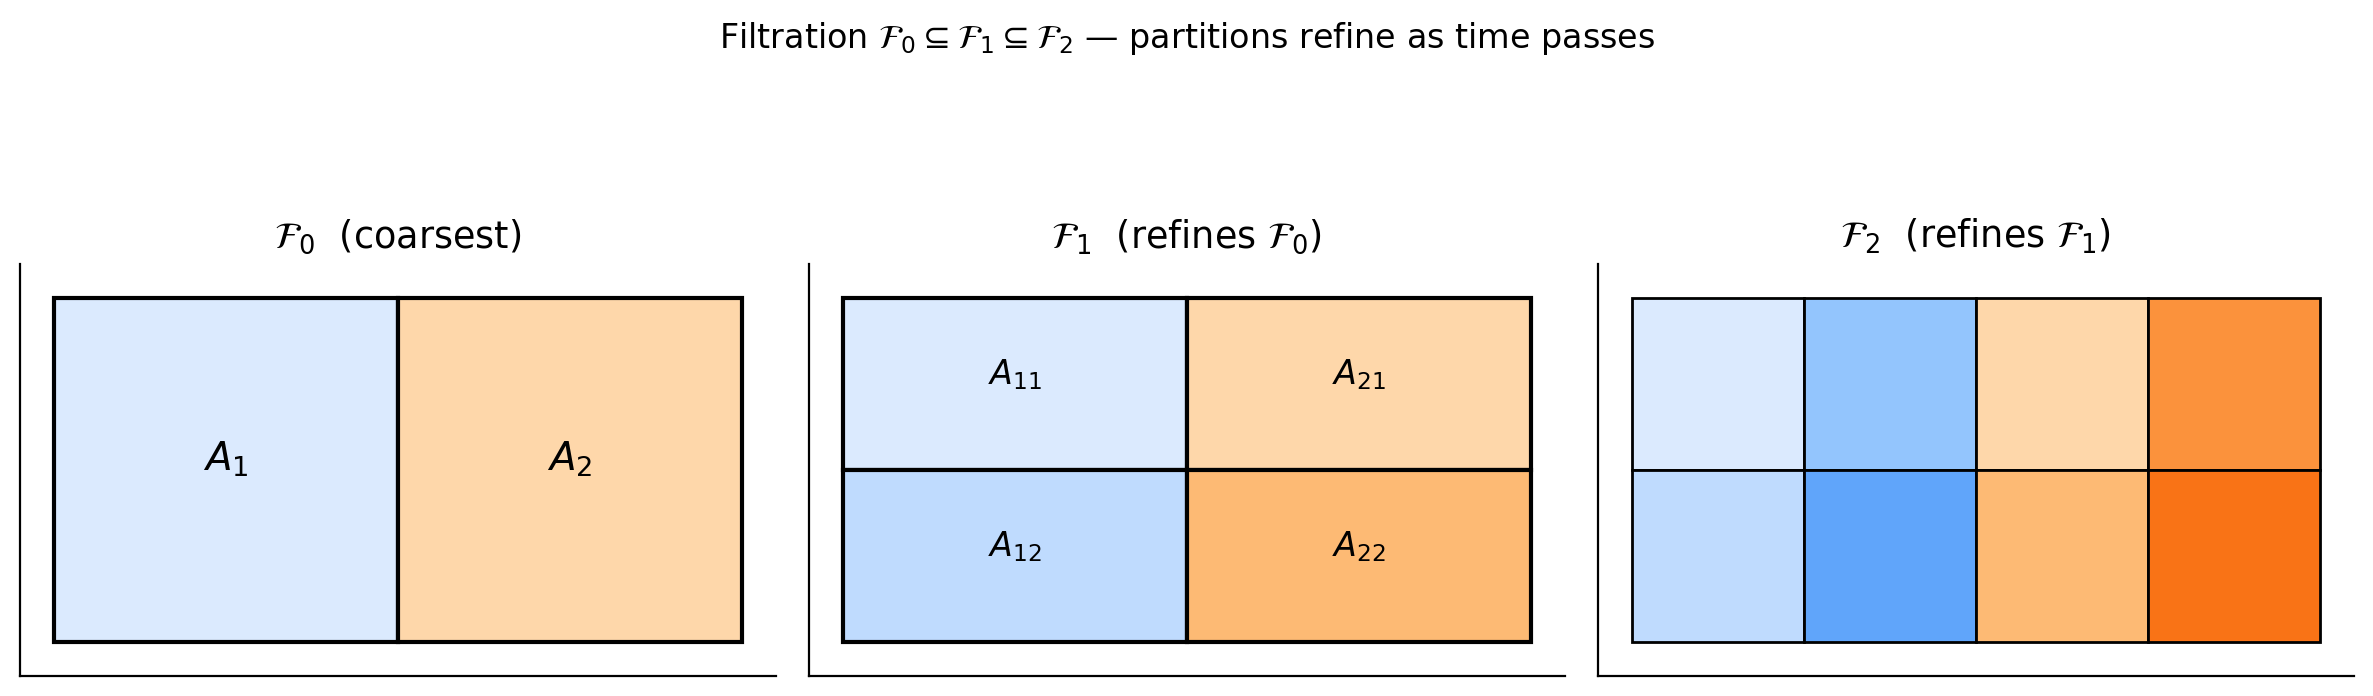
\includegraphics[keepaspectratio]{figures/ch00-sigma-refinement.png}}
\caption{Filtration
\(\mathcal{F}_0 \subseteq \mathcal{F}_1 \subseteq \mathcal{F}_2\) shown
as nested partition refinements --- the same intuition behind a daily
P\&L roll-up that, mid-session, splinters into hourly cells as more
information arrives}
\end{figure}

\emph{Almost surely} (a.s.) means ``with \(\mathbb{P}\)-probability 1'';
any random-variable equation in this guide is implicitly an a.s.
statement. \emph{Null sets} --- events with \(\mathbb{P} = 0\) --- are
ignorable; modifying \(X\) on a null set produces an a.s.-equal random
variable that behaves identically in every probabilistic computation.

\subsection{0.1.2 Conditional
expectation}\label{conditional-expectation}

Let \(\mathcal{G} \subseteq \mathcal{F}\) be a sub-\(\sigma\)-algebra.
The \textbf{conditional expectation} \(\mathbb{E}[X \mid \mathcal{G}]\)
is the unique (a.s.) \(\mathcal{G}\)-measurable random variable such
that

\[\int_A \mathbb{E}[X \mid \mathcal{G}]\, d\mathbb{P} = \int_A X\, d\mathbb{P} \quad \text{for every } A \in \mathcal{G}. \tag{0.1}\]

\emph{Intuition: \(\mathbb{E}[X \mid \mathcal{G}]\) is the best
\(L^2\)-prediction of \(X\) given the information in \(\mathcal{G}\).}
It is a random variable, not a number, because the prediction depends on
which \(\mathcal{G}\)-event was realised.

\begin{figure}
\centering
\pandocbounded{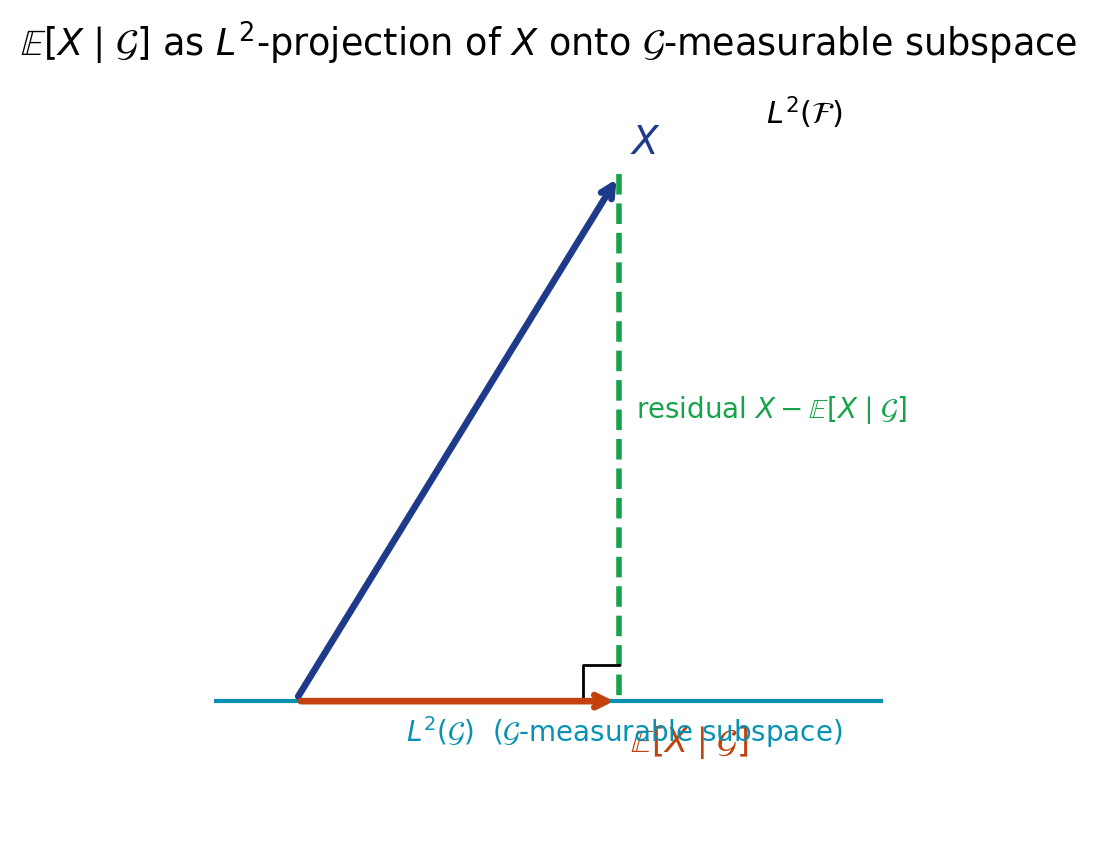
\includegraphics[keepaspectratio]{figures/ch00-cond-exp-projection.png}}
\caption{Conditional expectation as orthogonal projection of \(X\) onto
the \(\mathcal{G}\)-measurable subspace of \(L^2\); the residual
\(X - \mathbb{E}[X\mid\mathcal{G}]\) is the unhedgeable component ---
exactly the residual in a regression-based factor hedge}
\end{figure}

Three identities are used constantly in the rest of this guide.

\textbf{Tower property.} For
\(\mathcal{H} \subseteq \mathcal{G} \subseteq \mathcal{F}\),

\[\mathbb{E}\!\left[\mathbb{E}[X \mid \mathcal{G}] \,\big|\, \mathcal{H}\right] = \mathbb{E}[X \mid \mathcal{H}]. \tag{0.2}\]

\emph{Intuition: forecasting your own forecast based on less information
gives the less-informed forecast --- averaging is associative.}

\textbf{Taking out what is known.} If \(Y\) is
\(\mathcal{G}\)-measurable and integrable,

\[\mathbb{E}[Y X \mid \mathcal{G}] = Y \,\mathbb{E}[X \mid \mathcal{G}]. \tag{0.3}\]

\emph{Intuition: relative to \(\mathcal{G}\), the random variable \(Y\)
is a known constant and pulls out of the expectation.}

\textbf{Independence collapse.} If \(X\) is independent of
\(\mathcal{G}\), then
\(\mathbb{E}[X \mid \mathcal{G}] = \mathbb{E}[X]\). \emph{Intuition:
information you cannot use is no information at all.}

These three together do almost all the work in martingale arguments,
change-of-measure (Ch. 5), and tree-based pricing (Ch. 1, 2).

A numerical instance for (0.2). Let \(\xi_1, \xi_2\) be independent fair
\(\pm 1\) coin flips, \(X = \xi_1 + \xi_2\). Set
\(\mathcal{G} = \sigma(\xi_1)\) and
\(\mathcal{H} = \{\emptyset, \Omega\}\).

\begin{itemize}
\tightlist
\item
  \(\mathbb{E}[X \mid \mathcal{G}] = \xi_1 + \mathbb{E}[\xi_2] = \xi_1\).
\item
  \(\mathbb{E}[X \mid \mathcal{H}] = \mathbb{E}[X] = 0\).
\item
  Tower:
  \(\mathbb{E}[\xi_1 \mid \mathcal{H}] = 0 = \mathbb{E}[X \mid \mathcal{H}]\).
  ✓
\end{itemize}

Replace \(\xi\) with daily returns and \(\mathcal{G}, \mathcal{H}\) with
filtration timestamps and the same identity drives every multi-period
pricing argument in the guide.

\subsection{0.1.3 Independence vs
uncorrelatedness}\label{independence-vs-uncorrelatedness}

\(X\) and \(Y\) are \textbf{independent} iff
\(\mathbb{P}(X \in A, Y \in B) = \mathbb{P}(X \in A)\mathbb{P}(Y \in B)\)
for all measurable \(A, B\). They are \textbf{uncorrelated} iff
\(\mathbb{E}[XY] = \mathbb{E}[X]\mathbb{E}[Y]\).

Independence implies uncorrelated. The converse is false in general; it
is true only when \((X, Y)\) are jointly Gaussian.

\textbf{Counterexample.} Let \(X \sim N(0,1)\) and \(Y = X^2\). Then
\(\mathbb{E}[XY] = \mathbb{E}[X^3] = 0 = \mathbb{E}[X]\mathbb{E}[Y]\),
so \(X\) and \(Y\) are uncorrelated. But \(Y\) is a deterministic
function of \(X\); they are maximally dependent. \emph{Intuition:
correlation is a single linear summary; dependence has many non-linear
flavours that correlation cannot see.}

This matters in practice: a correlation matrix of returns being
near-diagonal does \emph{not} mean the assets are independent. Tail
co-movements (jointly large losses on bad days) live in the part of the
joint distribution that linear correlation discards. Copulas (briefly
touched in Ch. 15) are the right tool when you care about that.

\subsection{0.1.4 MGF, CGF, and the moment-generating
identity}\label{mgf-cgf-and-the-moment-generating-identity}

The \textbf{moment-generating function} of \(X\) is

\[M_X(t) = \mathbb{E}[e^{tX}], \qquad t \in \mathbb{R}, \tag{0.4}\]

defined wherever the expectation is finite. The
\textbf{cumulant-generating function} is \(K_X(t) = \log M_X(t)\).

Existence is not free. \(M_X(t)\) exists in an open neighbourhood of
\(0\) iff \(X\) has all moments and they grow at most exponentially fast
--- Gaussians have \(M\) everywhere, exponentials in a strip,
log-normals only at \(t \leq 0\) and never on a neighbourhood of \(0\).
\emph{That last point is the reason we use characteristic functions
\(\varphi_X(t) = \mathbb{E}[e^{itX}]\) rather than \(M_X\) in
heavy-tailed settings (Heston, Ch. 10).}

When \(M_X\) exists near \(0\), all moments are recovered by
differentiation:

\[\mathbb{E}[X^n] = \left.\frac{d^n M_X(t)}{dt^n}\right|_{t=0}, \qquad K_X(t) = \mu t + \tfrac{1}{2}\sigma^2 t^2 + \cdots \tag{0.5}\]

The Gaussian case is canonical:
\(X \sim N(\mu, \sigma^2) \Rightarrow M_X(t) = \exp(\mu t + \tfrac{1}{2}\sigma^2 t^2)\).
\emph{That \(\sigma^2/2\) is the same one that will appear as the Jensen
gap in §0.2 --- they are the same animal seen from different angles.}

\begin{figure}
\centering
\pandocbounded{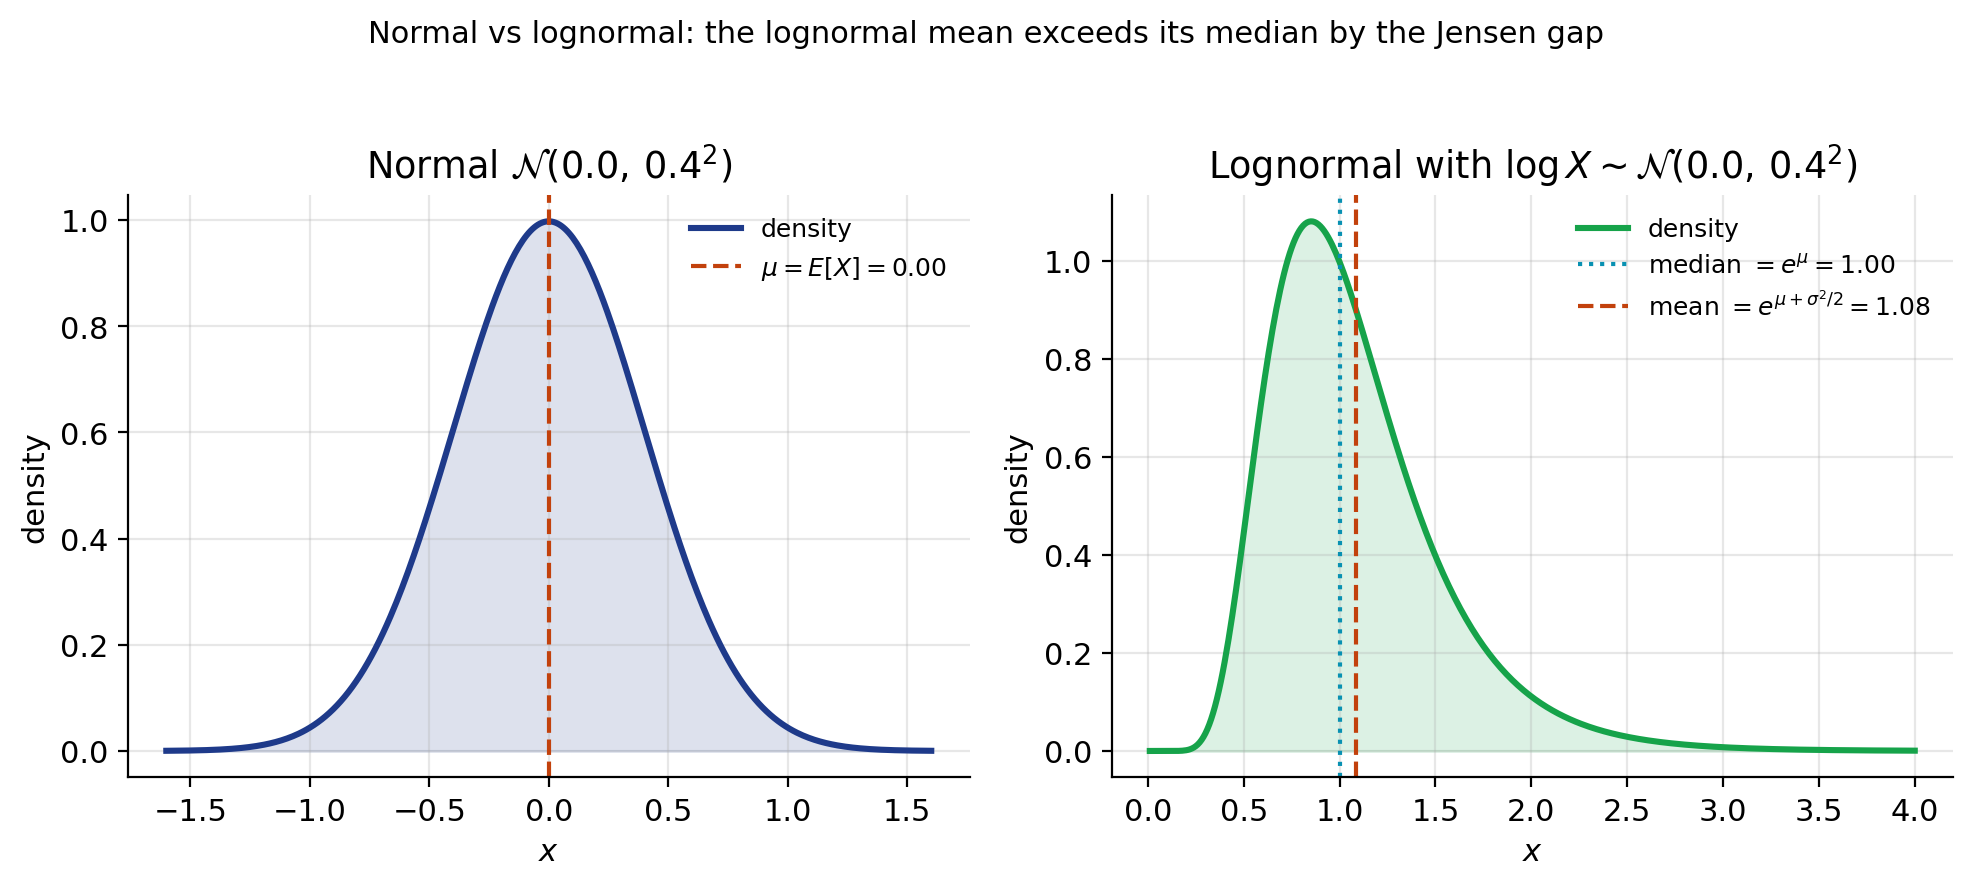
\includegraphics[keepaspectratio]{figures/ch00-normal-lognormal.png}}
\caption{Normal density of \(\log S\) versus the induced lognormal
density of \(S\); the lognormal mean exceeds its median by exactly the
Jensen gap \(e^{\sigma^2/2}-1\) --- the same multiplier that separates
``expected SPX level at T'' from ``median SPX level at T'' in equity
quotes}
\end{figure}

The CGF is more useful than the MGF when you want to read off cumulants
directly. For a Gaussian, \(K_X(t) = \mu t + \tfrac{1}{2}\sigma^2 t^2\)
--- a polynomial in \(t\) of degree 2, with all higher cumulants
vanishing. \emph{That fact (only the first two cumulants are non-zero)
is exactly the statement ``Gaussians are determined by mean and
variance,'' from a different vantage.} For a Poisson with rate
\(\lambda\), \(K(t) = \lambda(e^t - 1)\), infinitely many non-zero
cumulants --- Poisson is not even close to Gaussian. CGF additivity
\(K_{X+Y} = K_X + K_Y\) for independent \(X, Y\) is what makes them
computationally pleasant.

The \textbf{characteristic function}
\(\varphi_X(t) = \mathbb{E}[e^{itX}]\) always exists (the integrand has
modulus 1), unlike the MGF. It is the workhorse of Heston pricing (Ch.
10) and any Lévy-process model: when the MGF blows up, the CF still
works.

\subsection{0.1.5 Modes of convergence}\label{modes-of-convergence}

Let \(X_n, X\) be random variables on a common space.

{\def\LTcaptype{none} % do not increment counter
\begin{longtable}[]{@{}
  >{\raggedright\arraybackslash}p{(\linewidth - 2\tabcolsep) * \real{0.5000}}
  >{\raggedright\arraybackslash}p{(\linewidth - 2\tabcolsep) * \real{0.5000}}@{}}
\toprule\noalign{}
\begin{minipage}[b]{\linewidth}\raggedright
Mode
\end{minipage} & \begin{minipage}[b]{\linewidth}\raggedright
Definition
\end{minipage} \\
\midrule\noalign{}
\endhead
\bottomrule\noalign{}
\endlastfoot
Almost sure (a.s.) & \(\mathbb{P}(X_n \to X) = 1\) \\
In \(L^p\) & \(\mathbb{E}|X_n - X|^p \to 0\) \\
In probability & \(\mathbb{P}(|X_n - X| > \varepsilon) \to 0\) for all
\(\varepsilon > 0\) \\
In distribution & \(F_{X_n}(x) \to F_X(x)\) at all continuity points of
\(F_X\) \\
\end{longtable}
}

\begin{figure}
\centering
\pandocbounded{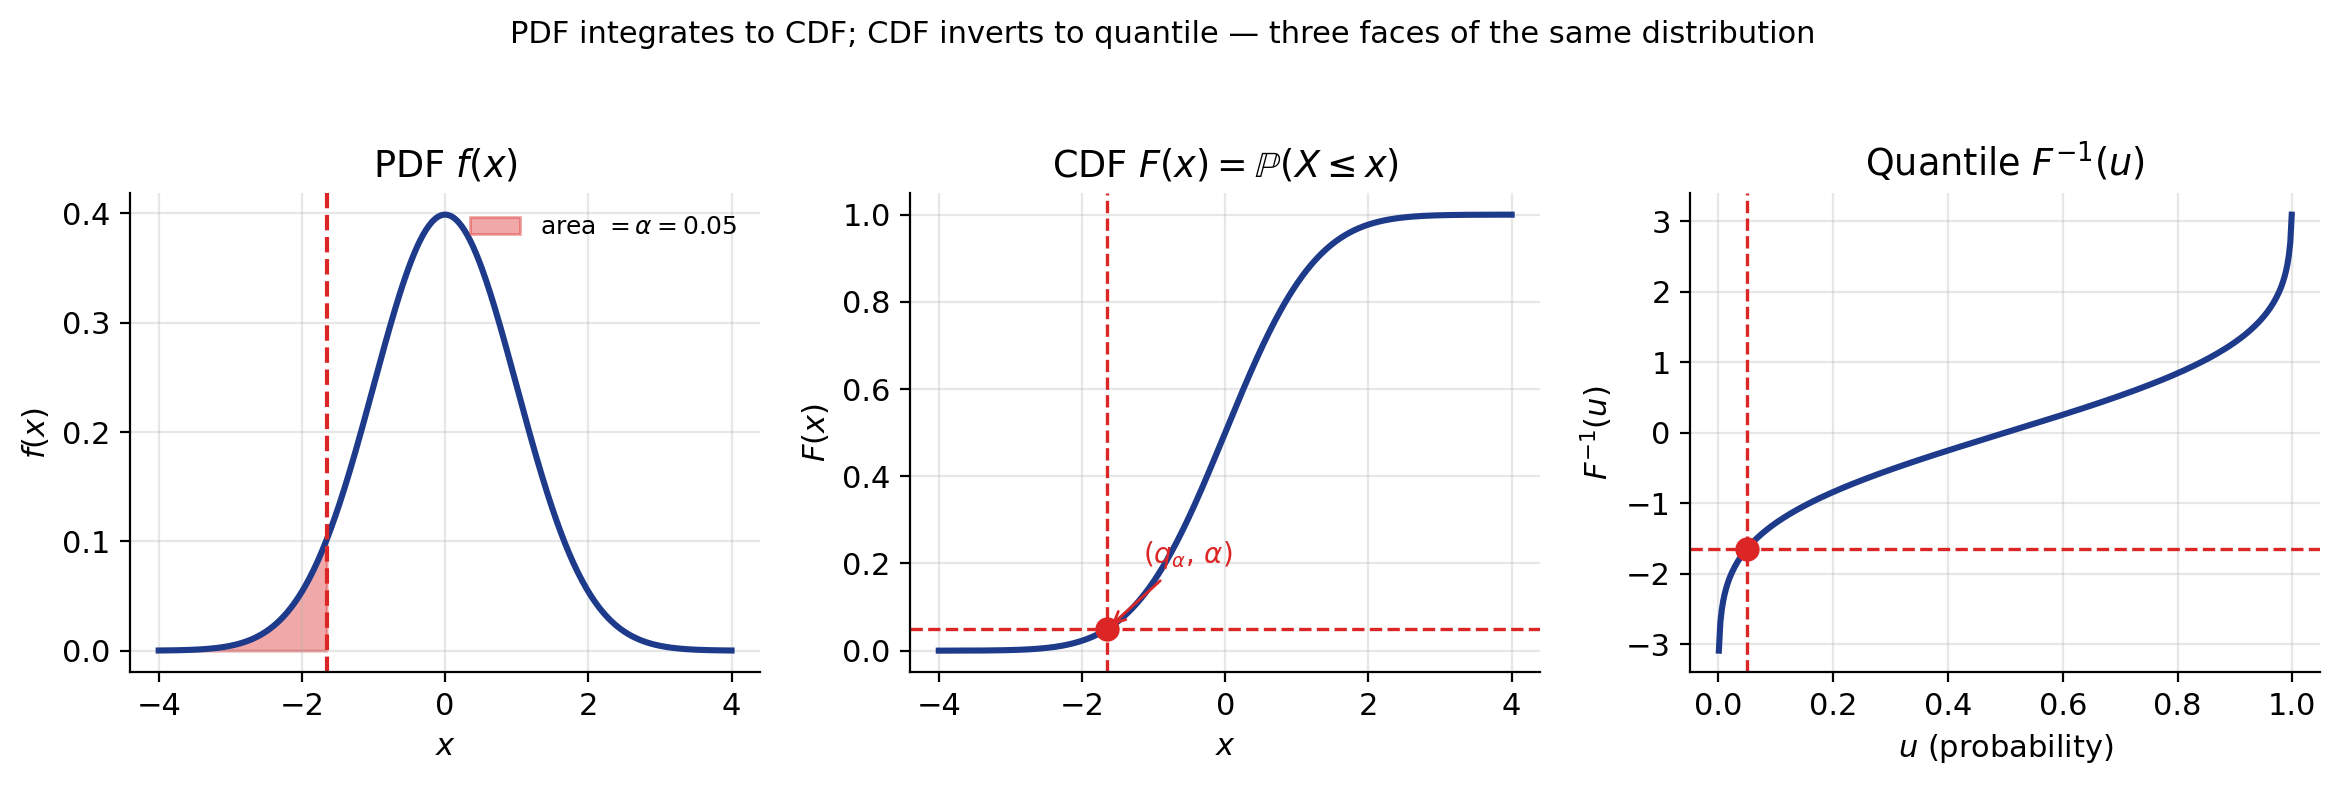
\includegraphics[keepaspectratio]{figures/ch00-cdf-pdf-quantile.png}}
\caption{PDF, CDF, and quantile function of \(\mathcal{N}(0,1)\)
side-by-side, with the same \(\alpha=5\%\) tail point marked on each ---
the operational picture behind any 95\% VaR calculation}
\end{figure}

The implication diagram (no other arrows hold in general):

\[\text{a.s.} \;\Longrightarrow\; \text{in probability} \;\Longrightarrow\; \text{in distribution}\]

\[L^p \;\Longrightarrow\; \text{in probability} \quad (p \geq 1)\]

\emph{Intuition: a.s. and \(L^p\) are both strong (they both control the
random variables themselves), but neither implies the other; both imply
convergence in probability, which is a weak pointwise control;
convergence in distribution is the weakest --- only marginal laws agree,
and the variables need not even live on the same space.}

\textbf{Practitioner consequence.} Monte Carlo (Ch. 9) gives \(L^2\) (or
even a.s. via the SLLN) convergence of sample means. The CLT gives
convergence in distribution of the rescaled error --- these are
different statements about different things.

\begin{figure}
\centering
\pandocbounded{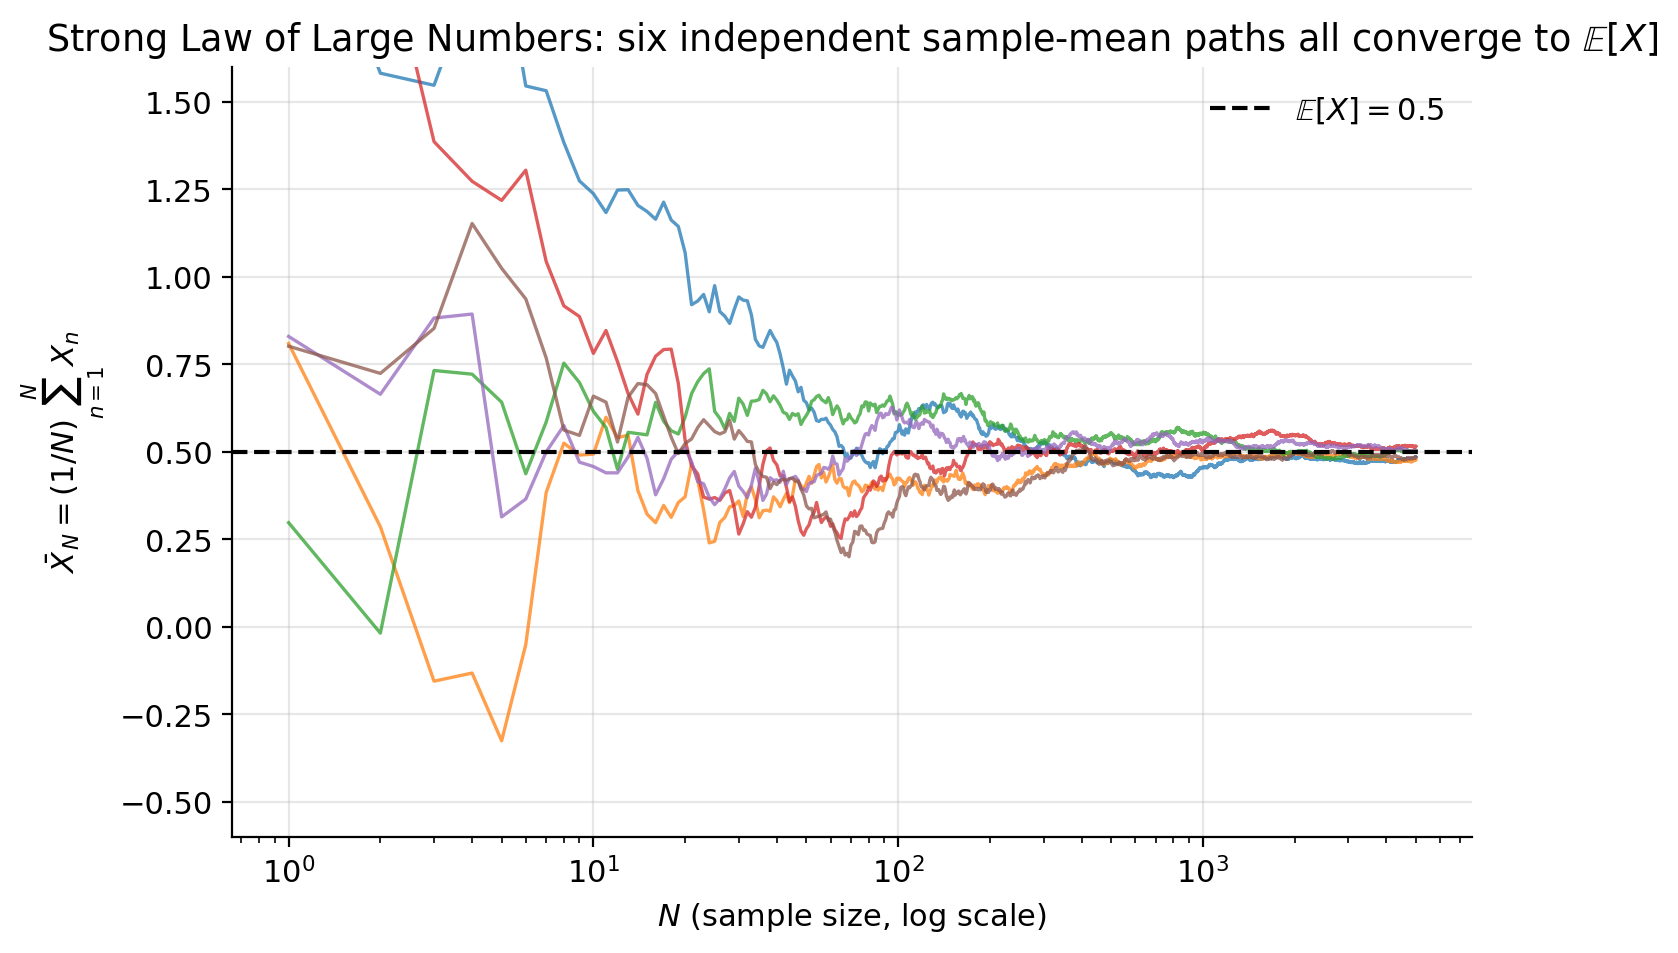
\includegraphics[keepaspectratio]{figures/ch00-lln-paths.png}}
\caption{Six independent sample-mean paths \(\bar X_N\) of Bernoulli
draws all funnel into \(\mathbb{E}[X]=0.5\) as \(N\) grows --- the SLLN
in action. Every Monte-Carlo option-pricing run is one of these paths,
and the spread at \(N=10^4\) is what the standard error bar reports}
\end{figure}

\begin{figure}
\centering
\pandocbounded{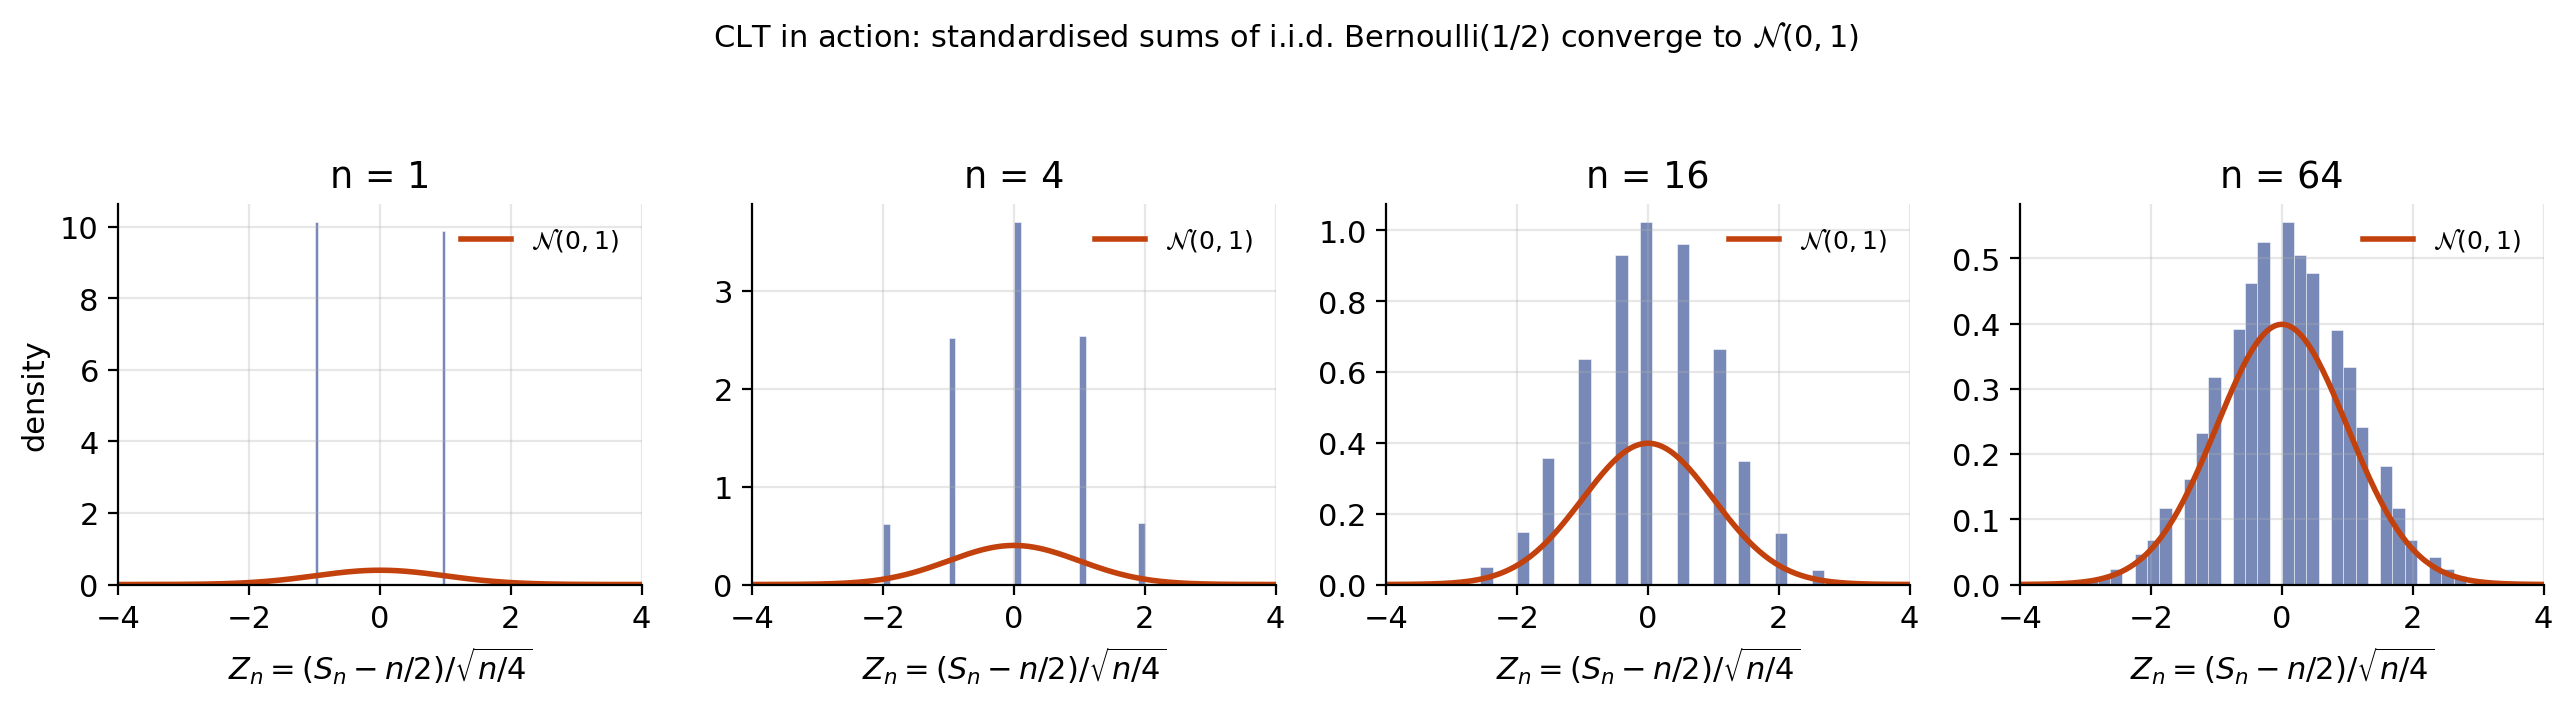
\includegraphics[keepaspectratio]{figures/ch00-clt-convergence.png}}
\caption{Standardised sums of Bernoulli(\(1/2\)) approach
\(\mathcal{N}(0,1)\) as \(n=1,4,16,64\) --- the CLT visualised. The same
convergence is why daily-return Z-scores aggregated over a quarter look
more Gaussian than the noisy raw daily distribution}
\end{figure}

A canonical separating example. Let \(X_n\) be independent with
\(\mathbb{P}(X_n = n^2) = 1/n\) and \(\mathbb{P}(X_n = 0) = 1 - 1/n\).
Then \(X_n \to 0\) in probability
(\(\mathbb{P}(X_n > \varepsilon) = 1/n \to 0\)) but
\(\mathbb{E}[X_n] = n \to \infty\), so \(X_n\) does \emph{not} converge
in \(L^1\). \emph{Intuition: a vanishingly rare but explosively large
outcome can leave probability convergence intact while breaking
expectation convergence.} This is exactly the failure mode of naïve
Monte Carlo on heavy-tailed payoffs (deep OTM puts on a jump-prone
asset, Ch. 9): sample means look like they converge, until one of the
rare extreme draws shows up and erases your average.

\begin{figure}
\centering
\pandocbounded{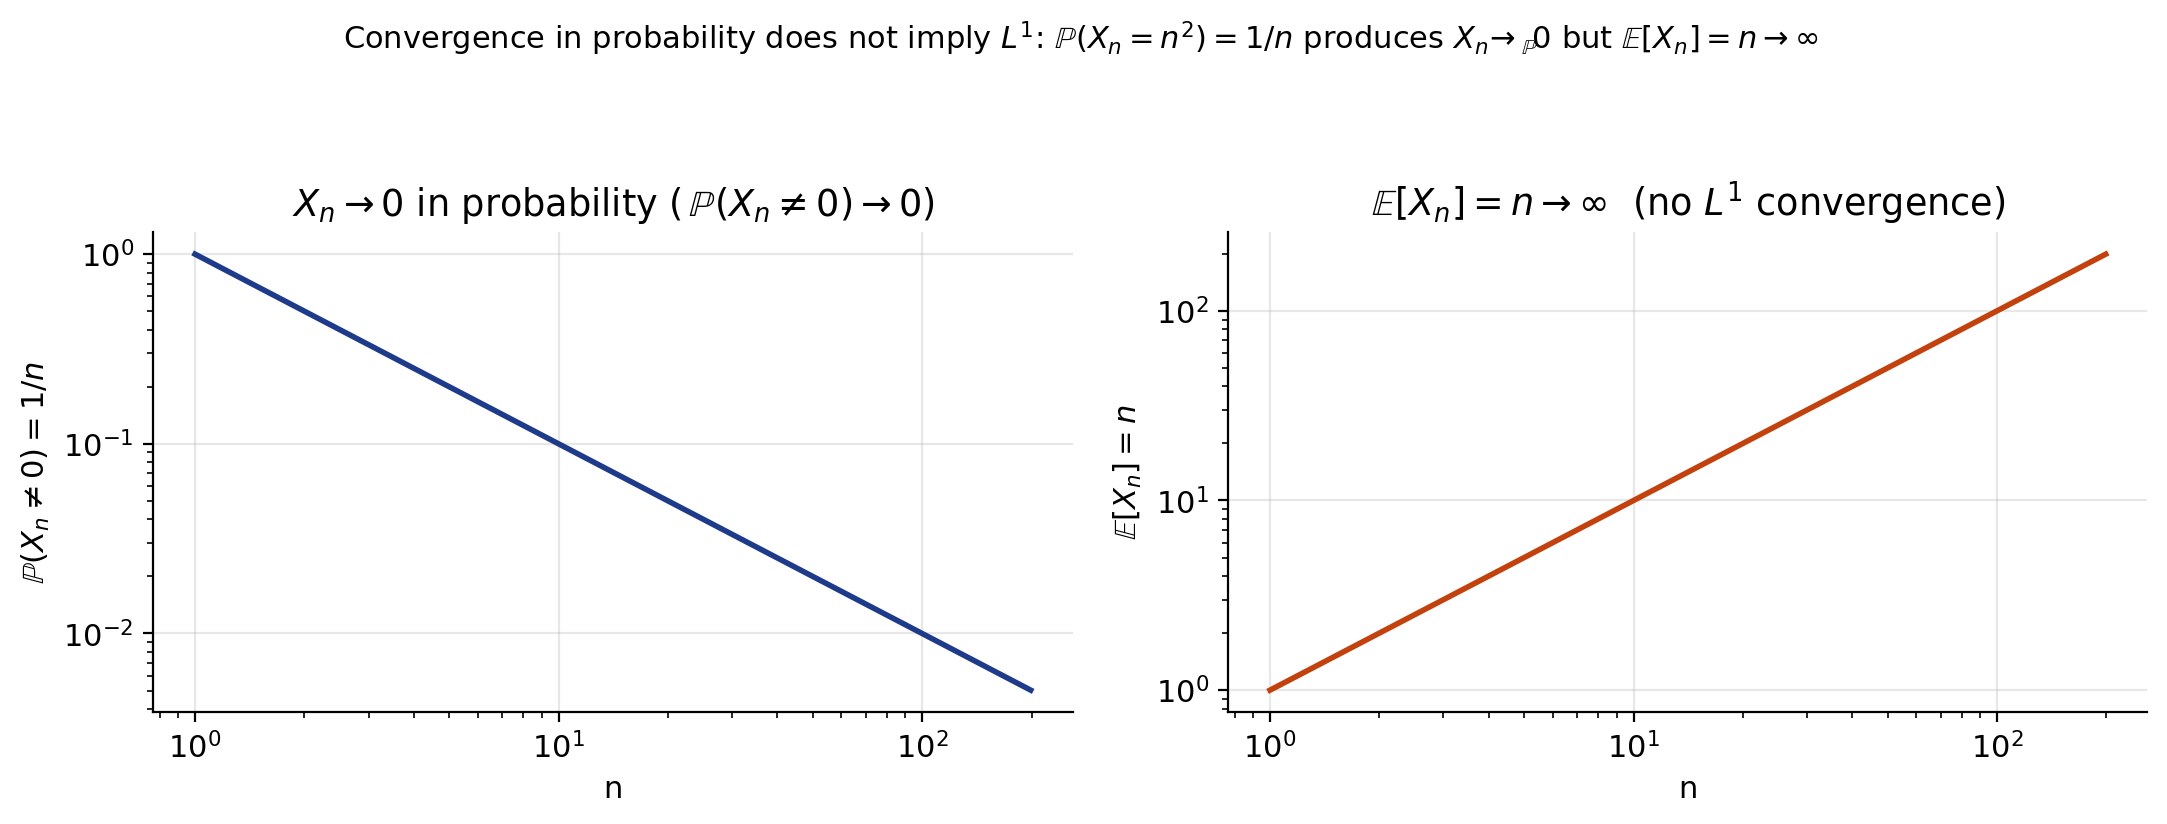
\includegraphics[keepaspectratio]{figures/ch00-mode-convergence.png}}
\caption{Separating example \(\mathbb{P}(X_n=n^2)=1/n\): convergence in
probability (\(1/n \to 0\), left panel) with simultaneous \(L^1\)
blow-up (\(\mathbb{E}[X_n] = n \to \infty\), right panel) --- the
textbook fingerprint of a ``deep-OTM put on an asset with jump risk'' MC
estimator that quietly diverges in mean while looking stable in median}
\end{figure}

\subsection{0.1.6 Borel--Cantelli}\label{borelcantelli}

Let \(\{A_n\}\) be a sequence of events. Define
\(\{A_n \text{ i.o.}\} = \bigcap_N \bigcup_{n \geq N} A_n\)
(``infinitely often'').

\textbf{BC-I.} If \(\sum_n \mathbb{P}(A_n) < \infty\), then
\(\mathbb{P}(A_n \text{ i.o.}) = 0\). \emph{Intuition: rare events with
finite total mass cannot happen infinitely often.}

\textbf{BC-II.} If \(\{A_n\}\) are independent and
\(\sum_n \mathbb{P}(A_n) = \infty\), then
\(\mathbb{P}(A_n \text{ i.o.}) = 1\). \emph{Intuition: independent
events with unbounded total mass must, by chance alone, eventually pile
up.}

These two together pin down the long-run behaviour of nearly every limit
theorem you will meet in the rest of this guide.

A trading-floor example. A strategy has a 1-in-100 chance of a 10-sigma
drawdown each day, independent across days. BC-II says: over an infinite
horizon the event happens infinitely often. Any non-zero per-period
probability of a tail event materialises with probability 1 over a long
enough horizon. Do not size positions as if the tail is ``unlikely this
year.''

\subsection{0.1.7 Two more workhorse
inequalities}\label{two-more-workhorse-inequalities}

\textbf{Markov's inequality.} For non-negative \(X\) and \(a > 0\),

\[\mathbb{P}(X \geq a) \leq \frac{\mathbb{E}[X]}{a}.\]

\emph{Intuition: non-negative random variables cannot put much mass far
above their mean --- the mean would have to be larger than it is.} This
is the seed of every concentration inequality.

\textbf{Chebyshev's inequality.} For \(X\) with finite variance,

\[\mathbb{P}(|X - \mu| \geq k\sigma) \leq \frac{1}{k^2}.\]

\emph{Intuition: variance bounds tail probability, distribution-free.}
For a Gaussian, the actual probability at \(k = 3\) is \(\sim 0.27\%\);
Chebyshev only gives \(\leq 11.1\%\). The bound is loose precisely
because it is distribution-free; the value is in proofs where you have
only a variance bound.

The Cauchy--Schwarz inequality
\(\mathbb{E}[XY]^2 \leq \mathbb{E}[X^2]\,\mathbb{E}[Y^2]\) rounds out
the basic kit; it is used implicitly any time you write
\(|\mathrm{Cov}(X,Y)| \leq \sigma_X \sigma_Y\) (the bound that defines
the correlation coefficient as living in \([-1,1]\)).

\begin{center}\rule{0.5\linewidth}{0.5pt}\end{center}

\section{\texorpdfstring{§0.2 Jensen's Inequality and the \(\sigma^2/2\)
Drift
Correction}{§0.2 Jensen's Inequality and the \textbackslash sigma\^{}2/2 Drift Correction}}\label{jensens-inequality-and-the-sigma22-drift-correction}

This is the most reused single fact in the guide. It appears in the GBM
log-drift, in the Itô correction (Ch. 3), in implied-vol convexity
adjustments (Ch. 7, 11), in convexity-adjusted forwards (Ch. 8), in
Black's caplet pricing (Ch. 14), and any time someone says ``geometric
mean \(\leq\) arithmetic mean'' --- they are quoting Jensen.

\subsection{0.2.1 The inequality}\label{the-inequality}

For a \textbf{convex} function \(f\) and integrable \(X\),

\[\mathbb{E}[f(X)] \;\geq\; f(\mathbb{E}[X]). \tag{0.6}\]

For \textbf{concave} \(f\), flip the inequality:

\[\mathbb{E}[f(X)] \;\leq\; f(\mathbb{E}[X]). \tag{0.7}\]

Equality holds iff \(f\) is affine on the support of \(X\), or \(X\) is
degenerate.

\subsection{0.2.2 Geometric intuition}\label{geometric-intuition}

Convexity means: any chord between two points on the graph of \(f\) lies
\emph{above} the graph between those points. Averaging two values of
\(f\) is taking a point on a chord; averaging the inputs and then
applying \(f\) is taking a point on the curve. The chord is above. So
\(\mathbb{E}[f(X)] \geq f(\mathbb{E}[X])\). Concave is the mirror image.

\begin{figure}
\centering
\pandocbounded{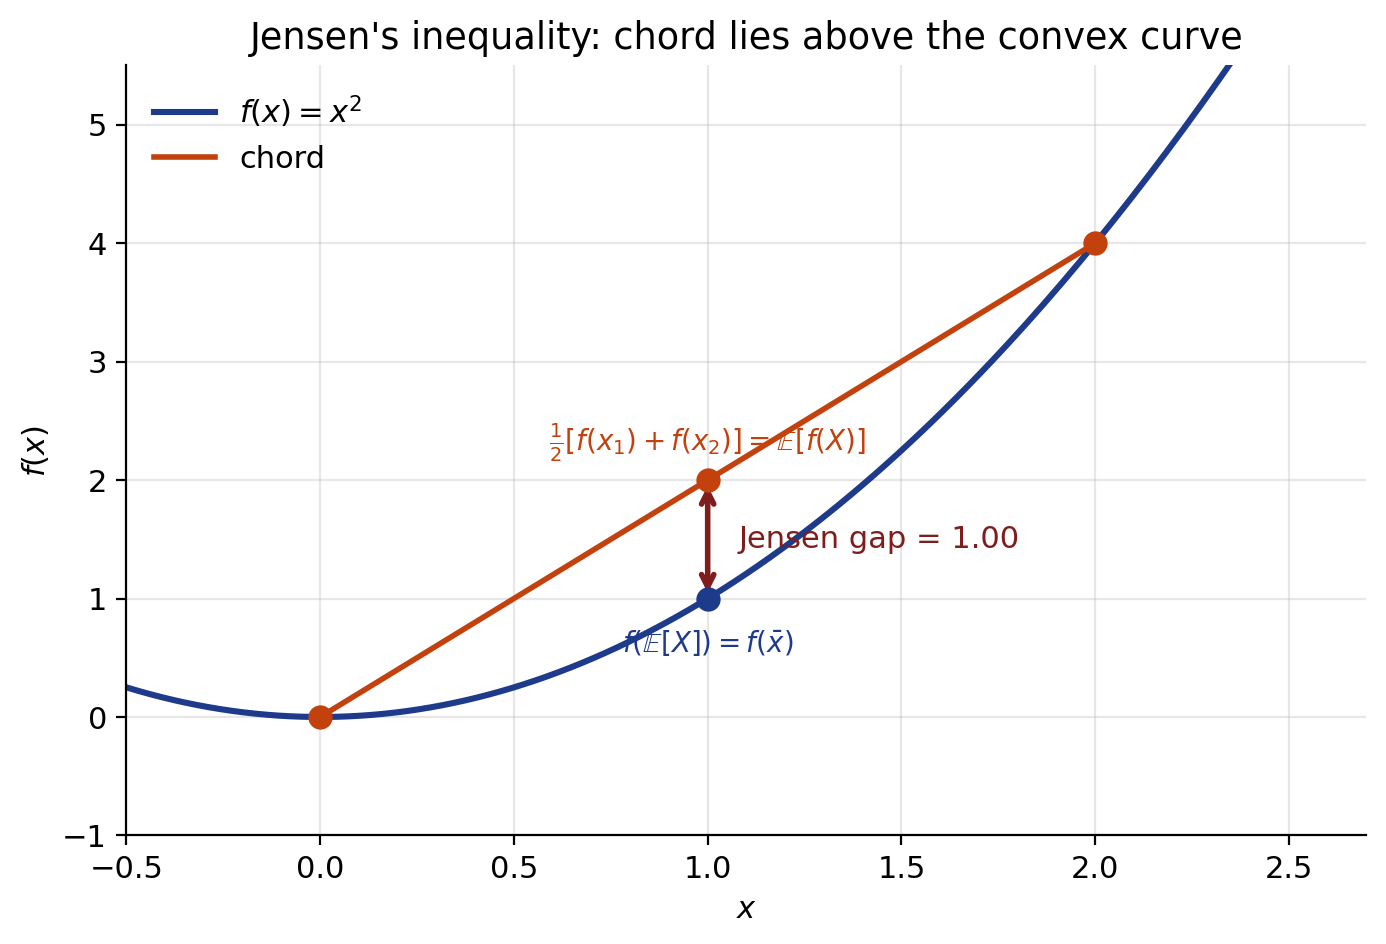
\includegraphics[keepaspectratio]{figures/ch00-jensen-chord.png}}
\caption{Convex \(f(x)=x^2\) with chord between \(x_1=0\) and \(x_2=2\):
the chord midpoint at \((1, 2)\) sits above the curve point \((1, 1)\)
--- the gap is exactly \(\sigma^2\) for symmetric \(\pm 1\) noise around
\(\mathbb{E}[X]=1\) (here \(\sigma^2=1\), matching the unit gap)}
\end{figure}

This is not a measure-theoretic fact; it is a statement about chords and
curves. The \(\mathbb{E}\) does the integration, but the \emph{gap} is
geometric --- a function of how curvy \(f\) is and how spread out \(X\)
is.

\subsection{\texorpdfstring{0.2.3 The \(\sigma^2/2\) worked
example}{0.2.3 The \textbackslash sigma\^{}2/2 worked example}}\label{the-sigma22-worked-example}

Let \(S\) be log-normal: \(\log S \sim N(\mu, \sigma^2)\). Then
\(S = e^{\log S}\) where \(\log S\) is Gaussian. Compute the three
relevant quantities.

\textbf{Expected value of \(S\).} Using the Gaussian MGF (0.5) at
\(t=1\),

\[\mathbb{E}[S] = \mathbb{E}[e^{\log S}] = M_{\log S}(1) = \exp\!\left(\mu + \tfrac{1}{2}\sigma^2\right). \tag{0.8}\]

\textbf{Log of the expected value.}

\[\log \mathbb{E}[S] = \mu + \tfrac{1}{2}\sigma^2. \tag{0.9}\]

\textbf{Expected value of the log.}

\[\mathbb{E}[\log S] = \mu. \tag{0.10}\]

\textbf{The Jensen gap.} Subtracting (0.10) from (0.9):

\[\boxed{\log \mathbb{E}[S] - \mathbb{E}[\log S] = \tfrac{1}{2}\sigma^2.} \tag{0.11}\]

This is Jensen's inequality with \(f = \log\) (concave):
\(\mathbb{E}[\log S] \leq \log \mathbb{E}[S]\), with the gap exactly
\(\sigma^2/2\) for the log-normal.

\emph{Intuition: the gap measures how much the log function bends over
the support of \(S\). Small \(\sigma\) means \(S\) is concentrated near
its mean and the function is nearly linear there --- small gap. Large
\(\sigma\) probes wider regions where \(\log\) is much more curved ---
large gap. The factor \(1/2\) comes from the second derivative of
\(\log\), just as the \(1/2\) in the Taylor expansion of
\(\log(1+x) \approx x - x^2/2\) does.}

\subsection{0.2.4 Connection to GBM and the Itô drift
correction}\label{connection-to-gbm-and-the-ituxf4-drift-correction}

Geometric Brownian motion under measure \(\mathbb{P}\):

\[dS_t = \mu S_t\, dt + \sigma S_t\, dW_t, \qquad S_0 \text{ given.} \tag{0.12}\]

The integrated solution (anticipating Ch. 3's Itô calculus, but the
result is what matters here) is

\[S_T = S_0 \exp\!\left[\left(\mu - \tfrac{1}{2}\sigma^2\right)T + \sigma W_T\right]. \tag{0.13}\]

Two expectations to take:

\[\mathbb{E}[S_T] = S_0 e^{\mu T}, \tag{0.14}\]

\[\mathbb{E}\!\left[\log\!\frac{S_T}{S_0}\right] = \left(\mu - \tfrac{1}{2}\sigma^2\right) T. \tag{0.15}\]

The \(\sigma^2/2\) in the log-drift in (0.13) and (0.15) is \emph{not} a
math glitch. It is exactly the Jensen gap (0.11) at \(T=1\) with
\(\sigma\) replaced by \(\sigma\sqrt{T}\):

\[\log \mathbb{E}[S_T/S_0] - \mathbb{E}[\log(S_T/S_0)] = \mu T - (\mu - \tfrac{1}{2}\sigma^2) T = \tfrac{1}{2}\sigma^2 T. \tag{0.16}\]

The same correction appears as the second-order term in Itô's lemma
applied to \(\log S\): the deterministic chain rule would give
\(d(\log S) = dS/S\), but Itô adds \(-\tfrac{1}{2}\sigma^2 dt\) because
\(dW^2 = dt\) does not vanish (Ch. 3, §3.4). \emph{Three names for one
phenomenon: Jensen's gap, the GBM log-drift correction, the Itô
second-order term.}

\subsection{0.2.5 A real number}\label{a-real-number}

Take \(\mu = 8\%\), \(\sigma = 30\%\), \(T = 1\) year.

{\def\LTcaptype{none} % do not increment counter
\begin{longtable}[]{@{}
  >{\raggedright\arraybackslash}p{(\linewidth - 4\tabcolsep) * \real{0.3333}}
  >{\raggedright\arraybackslash}p{(\linewidth - 4\tabcolsep) * \real{0.3333}}
  >{\raggedright\arraybackslash}p{(\linewidth - 4\tabcolsep) * \real{0.3333}}@{}}
\toprule\noalign{}
\begin{minipage}[b]{\linewidth}\raggedright
Quantity
\end{minipage} & \begin{minipage}[b]{\linewidth}\raggedright
Formula
\end{minipage} & \begin{minipage}[b]{\linewidth}\raggedright
Value
\end{minipage} \\
\midrule\noalign{}
\endhead
\bottomrule\noalign{}
\endlastfoot
Arithmetic mean of \(S_T/S_0\) & \(e^{\mu T}\) &
\(e^{0.08} = 1.0833\) \\
Geometric mean of \(S_T/S_0\) & \(e^{(\mu - \sigma^2/2)T}\) &
\(e^{0.08 - 0.045} = e^{0.035} = 1.0356\) \\
Log of arithmetic mean & \(\mu T\) & \(0.0800\) \\
Mean of log return & \((\mu - \sigma^2/2)T\) & \(0.0350\) \\
Jensen gap & \(\sigma^2 T / 2\) & \(0.0450\) \\
\end{longtable}
}

The arithmetic mean exceeds the geometric mean by \(\sim 4.7\%\), almost
exactly \(\sigma^2/2 = 4.5\%\) (the small extra is the higher-order
curvature of \(\exp\)). \emph{In a year of 30-vol equity, the ``expected
return'' of 8\% and the ``median compounded return'' of 3.5\% are both
correct statements about the same process. They differ by Jensen's gap.}

\subsection{0.2.6 Practitioner aside}\label{practitioner-aside}

This is why CAGR is always less than the arithmetic mean of annual
returns for any non-trivial vol.~Pension reports quote CAGR; sales decks
quote arithmetic average; both are technically right and describe
different things. Volatility is a \emph{drag} on compounded wealth even
when expected returns are positive --- the Kelly drift
\(\mu - \sigma^2/2\) can be negative when \(\sigma^2 > 2\mu\). Every
time you see \(\mu - \sigma^2/2\), \(r - q - \sigma^2/2\), or
\(\sigma^2/2\) floating around alone, it is Jensen.

\subsection{0.2.7 The Jensen gap as a Taylor
expansion}\label{the-jensen-gap-as-a-taylor-expansion}

A second route to (0.6) makes the size of the gap quantitative. Expand
\(f\) around \(\mu = \mathbb{E}[X]\):

\[f(X) = f(\mu) + f'(\mu)(X - \mu) + \tfrac{1}{2} f''(\mu)(X - \mu)^2 + \text{higher order.} \tag{0.17}\]

Take expectations:

\[\mathbb{E}[f(X)] = f(\mu) + \tfrac{1}{2} f''(\mu)\,\mathrm{Var}(X) + \text{higher cumulants.} \tag{0.18}\]

The first-order term vanishes (\(\mathbb{E}[X - \mu] = 0\)); the
second-order term is exactly the Jensen gap to leading order, and it is
\textbf{proportional to \(f''(\mu)\) times the variance of \(X\)}.
\emph{Intuition: the gap is the curvature of \(f\) times the spread of
\(X\) --- both have to be present, and the gap grows linearly in each.}

For \(f = \log\) at \(\mu\), \(f''(\mu) = -1/\mu^2\), so the
leading-order log-gap is
\(-\tfrac{1}{2}\mathrm{Var}(X)/\mu^2 = -\tfrac{1}{2} \mathrm{CV}^2\)
where \(\mathrm{CV}\) is the coefficient of variation. For log-normal
\(X\) with log-vol \(\sigma\) this is \emph{exactly} \(-\sigma^2/2\) (no
higher-order error) because the third and higher cumulants of \(\log X\)
are zero --- the log of a log-normal is exactly Gaussian. \emph{That is
why the Jensen gap for log-normal is closed-form: the Taylor expansion
truncates.}

For non-Gaussian distributions the gap has corrections involving
skewness and higher cumulants, and Black--Scholes (which prices as if
returns were Gaussian) gets the gap ``wrong'' precisely in proportion to
the realised skew and kurt of the return distribution. That mismatch is
the entire content of the implied-volatility skew (Ch. 7, 11).

\subsection{0.2.8 Sign rules to memorise}\label{sign-rules-to-memorise}

Three sign conventions trip people up. Memorise them.

{\def\LTcaptype{none} % do not increment counter
\begin{longtable}[]{@{}
  >{\raggedright\arraybackslash}p{(\linewidth - 2\tabcolsep) * \real{0.5000}}
  >{\raggedright\arraybackslash}p{(\linewidth - 2\tabcolsep) * \real{0.5000}}@{}}
\toprule\noalign{}
\begin{minipage}[b]{\linewidth}\raggedright
Setting
\end{minipage} & \begin{minipage}[b]{\linewidth}\raggedright
Sign of \(\sigma^2/2\) correction
\end{minipage} \\
\midrule\noalign{}
\endhead
\bottomrule\noalign{}
\endlastfoot
GBM log-drift: \(\log S_T = (\mu - \sigma^2/2) T + \sigma W_T\) &
minus \\
Expected forward: \(\mathbb{E}[S_T] = S_0 e^{\mu T}\) & none (Jensen has
done its work in the log) \\
Itô-corrected drift of \(\log S\) & minus \\
Black's formula log-moneyness:
\(d_\pm = (\log(F/K) \pm \sigma^2 T/2)/(\sigma \sqrt T)\) & \(\pm\)
depending on \(d_+\) vs \(d_-\) \\
Convexity adjustment, futures vs forward (positive \(\rho\) between rate
and asset) & plus to the futures price \\
\end{longtable}
}

If you forget the sign in a hurry: \textbf{in the log of a log-normal,
the bias is a subtraction; in the level of a log-normal, the bias has
already been baked in.}

\subsection{0.2.9 Volatility drag and the Kelly
drift}\label{volatility-drag-and-the-kelly-drift}

The ``Kelly drift'' \(\mu - \sigma^2/2\) is the expected log-return per
unit time, also known as the \textbf{geometric growth rate} of the
asset. It is what compounds your money. The arithmetic drift \(\mu\) is
what enters the \emph{expected} terminal wealth but not the
\emph{typical} terminal wealth.

Two assets:

\begin{itemize}
\tightlist
\item
  Asset A: \(\mu = 12\%\), \(\sigma = 50\%\).
\item
  Asset B: \(\mu = 8\%\), \(\sigma = 15\%\).
\end{itemize}

{\def\LTcaptype{none} % do not increment counter
\begin{longtable}[]{@{}
  >{\raggedright\arraybackslash}p{(\linewidth - 4\tabcolsep) * \real{0.3333}}
  >{\raggedright\arraybackslash}p{(\linewidth - 4\tabcolsep) * \real{0.3333}}
  >{\raggedright\arraybackslash}p{(\linewidth - 4\tabcolsep) * \real{0.3333}}@{}}
\toprule\noalign{}
\begin{minipage}[b]{\linewidth}\raggedright
\end{minipage} & \begin{minipage}[b]{\linewidth}\raggedright
Asset A
\end{minipage} & \begin{minipage}[b]{\linewidth}\raggedright
Asset B
\end{minipage} \\
\midrule\noalign{}
\endhead
\bottomrule\noalign{}
\endlastfoot
Arithmetic drift \(\mu\) & 12\% & 8\% \\
Volatility \(\sigma\) & 50\% & 15\% \\
Variance drag \(\sigma^2/2\) & 12.5\% & 1.1\% \\
Geometric growth \(\mu - \sigma^2/2\) & \(-0.5\%\) & \(6.9\%\) \\
Expected wealth multiple after 30y & \(e^{3.6} = 36.6\times\) &
\(e^{2.4} = 11.0\times\) \\
Median wealth multiple after 30y & \(e^{-0.15} = 0.86\times\) &
\(e^{2.07} = 7.9\times\) \\
\end{longtable}
}

\emph{Asset A has a higher expected return and a higher expected
terminal wealth, but a typical (median) trajectory of Asset A loses
money over 30 years.} The mean is dragged up by a small probability of
enormous outcomes; the median, which is what an actual investor
experiences with high probability, is dictated by the geometric drift.
This is the volatility drag, and it is why position sizing (Kelly
fraction, risk parity) cares about \(\sigma^2/2\) as much as it cares
about \(\mu\). \emph{Picking strategies on raw \(\mu\) is selecting for
the assets whose Jensen gap will eat their typical performance.}

\begin{center}\rule{0.5\linewidth}{0.5pt}\end{center}

\section{§0.3 Stochastic-Process
Priming}\label{stochastic-process-priming}

A \textbf{stochastic process} is a family of random variables
\(\{X_t\}_{t \in T}\) on a common probability space, indexed by time
\(T \subseteq \mathbb{R}_+\). We work in continuous time throughout the
guide; the binomial model of Ch. 1--2 is the discrete-time analogue.

\subsection{0.3.1 Filtrations}\label{filtrations}

A \textbf{filtration} \(\{\mathcal{F}_t\}_{t \geq 0}\) is an increasing
family of \(\sigma\)-algebras: \(\mathcal{F}_s \subseteq \mathcal{F}_t\)
for \(s \leq t\).

\emph{Intuition: \(\mathcal{F}_t\) is what you know by date \(t\).
Information accumulates; you never forget.} The natural filtration of a
process \(X\) is \(\mathcal{F}_t^X = \sigma(X_s : s \leq t)\) --- the
smallest \(\sigma\)-algebra making the entire history of \(X\) up to
\(t\) measurable.

A process \(X\) is \textbf{adapted} to \(\{\mathcal{F}_t\}\) if \(X_t\)
is \(\mathcal{F}_t\)-measurable for every \(t\). \emph{Intuition:
adapted means ``you can read off \(X_t\) at time \(t\), not earlier.''}

A process \(X\) is \textbf{predictable} if \(X_t\) is
\(\mathcal{F}_{t-}\)-measurable --- known just before \(t\).
\emph{Intuition: a hedging strategy is predictable; you choose your
position based on the past, not on the increment you are about to
absorb.}

\subsection{0.3.2 Martingales}\label{martingales}

An adapted, integrable process \(M\) is a \textbf{martingale} if

\[\mathbb{E}[M_t \mid \mathcal{F}_s] = M_s, \qquad s \leq t. \tag{0.19}\]

A \textbf{submartingale} has \(\geq\), a \textbf{supermartingale} has
\(\leq\).

\emph{Intuition: a martingale is a fair game --- your best forecast of
tomorrow's value, given everything you know today, is today's value. A
submartingale drifts up on average; a supermartingale drifts down.}

Three canonical examples used throughout the guide:

\textbf{Brownian motion.} \(W_t\) is a martingale under its own
filtration: \(\mathbb{E}[W_t \mid \mathcal{F}_s] = W_s\) because
\(W_t - W_s\) is independent of \(\mathcal{F}_s\) with mean \(0\). So is
\(W_t^2 - t\) (the \emph{compensated quadratic variation}) --- Brownian
motion has variance growing as \(t\), and \(W_t^2 - t\) is the part with
the trend removed.

\textbf{Compensated Poisson.} If \(N_t\) is a Poisson process with rate
\(\lambda\), then \(N_t - \lambda t\) is a martingale. \emph{The
compensator \(\lambda t\) removes the deterministic drift; what remains
is a fair game of jump shocks.} Any jump model (Merton, Kou,
variance-gamma) builds a tradable asset by attaching this kind of
compensation so the discounted price is a \(\mathbb{Q}\)-martingale.

\textbf{Discounted prices under \(\mathbb{Q}\).} The fundamental theorem
of asset pricing (FTAP, Ch. 2) says: a market is arbitrage-free iff
there exists a measure \(\mathbb{Q}\) under which discounted asset
prices \(S_t / B_t\) are martingales, where \(B_t\) is the numéraire
(typically the money-market account). \emph{Intuition: under
\(\mathbb{Q}\), no asset systematically out-earns the numéraire --- that
is exactly what ``no arbitrage'' means.}

\subsection{0.3.3 Markov property}\label{markov-property}

A process \(X\) is \textbf{Markov} if for any \(s \leq t\) and bounded
measurable \(f\),

\[\mathbb{E}[f(X_t) \mid \mathcal{F}_s] = \mathbb{E}[f(X_t) \mid X_s]. \tag{0.20}\]

\emph{Intuition: the future depends on the past only through the present
--- knowing the full history is no better than knowing the current
state.}

Markov is what makes PDEs work for option pricing (Ch. 4, 6): the option
price at \((t, S_t)\) depends only on \((t, S_t)\), not on the whole
path of \(S\). Heston (Ch. 10) is Markov in the \emph{pair}
\((S_t, V_t)\) but not in \(S_t\) alone --- that is why Heston needs a
2-D PDE and a 2-D characteristic function.

\subsection{0.3.4 Stopping times}\label{stopping-times}

A random time \(\tau : \Omega \to [0, \infty]\) is a \textbf{stopping
time} if \(\{\tau \leq t\} \in \mathcal{F}_t\) for every \(t\).

\emph{Intuition: \(\tau\) is a stopping time iff you can decide whether
to stop using only the information available up to \(t\) --- no
peeking.}

The first hitting time of a Brownian motion at level \(a\),
\(\tau = \inf\{t : W_t = a\}\), is a stopping time. The time of the
\emph{maximum} of \(W\) over \([0, T]\) is \emph{not} --- to know it,
you would have to know the future.

Stopping times are how American options (early exercise) and barrier
options are formalised: the exercise time of an American option is a
stopping time chosen to maximise expected discounted payoff under
\(\mathbb{Q}\).

Two further properties used later. (i) The min and max of two stopping
times are stopping times --- you can compose decisions (``stop at the
first knock-out \emph{or} maturity''). (ii) The \textbf{stopped
\(\sigma\)-algebra}
\(\mathcal{F}_\tau = \{A : A \cap \{\tau \leq t\} \in \mathcal{F}_t \,\forall t\}\)
is the information available up to the random time \(\tau\). Optional
sampling extends the martingale property to such random times.

\subsection{0.3.5 Optional sampling
theorem}\label{optional-sampling-theorem}

If \(M\) is a uniformly integrable martingale and \(\sigma \leq \tau\)
are bounded stopping times, then

\[\mathbb{E}[M_\tau \mid \mathcal{F}_\sigma] = M_\sigma. \tag{0.21}\]

\emph{Intuition: the martingale property survives even if you stop at a
smart, information-respecting random time. ``No clever stopping rule
beats a fair game.''}

The boundedness or UI condition is essential --- without it, doubling
strategies break the conclusion. This theorem is what makes the FTAP
arguments of Ch. 2 work in the multi-period setting.

\subsection{0.3.6 Doob decomposition}\label{doob-decomposition}

Any submartingale \(X\) decomposes uniquely as

\[X_t = M_t + A_t \tag{0.22}\]

with \(M\) a martingale and \(A\) a predictable, increasing process with
\(A_0 = 0\).

\emph{Intuition: every ``drifting up'' process is a fair game plus a
foreseeable upward drift; the decomposition separates the risk from the
trend.} In continuous time this is the Doob--Meyer decomposition; for an
Itô process, \(A_t = \int_0^t (\text{drift})\, ds\) and
\(M_t = \int_0^t (\text{volatility})\, dW_s\). The Doob decomposition is
the abstract generalisation of ``drift plus diffusion.''

\subsection{0.3.7 Quadratic variation}\label{quadratic-variation}

For a continuous semi-martingale \(X\), the \textbf{quadratic variation}
\([X]_t\) is the limit (in probability) of
\(\sum (X_{t_{i+1}} - X_{t_i})^2\) over partitions of \([0, t]\) as the
mesh shrinks to zero.

For Brownian motion, \([W]_t = t\). \emph{Intuition: increments of size
\(\sqrt{dt}\) squared and summed over \(1/dt\) intervals give
\(dt \cdot 1/dt = 1\) per unit time.} Compare to a smooth function,
whose quadratic variation is zero (smooth wiggles squared sum to
nothing). That non-zero quadratic variation is exactly what powers Itô
calculus.

For correlated Brownians \(W^1, W^2\) with correlation \(\rho\), the
cross-variation is \([W^1, W^2]_t = \rho t\). \emph{This is the
continuous-time content of ``Cov is bilinear in increments.''} Itô's
lemma in two variables is built on this identity.

A last fact for Ch. 3: for any Itô process
\(dX = \mu_t\, dt + \sigma_t\, dW_t\), the quadratic variation is
\([X]_t = \int_0^t \sigma_s^2\, ds\). \emph{The drift contributes
nothing --- drift is smooth, only the noise has quadratic variation.}
This is the realised-variance estimator of stochastic vol models (Ch.
10) made formal: integrated variance is the quadratic variation of
log-price.

\subsection{0.3.8 Itô's formula in advance, in one
line}\label{ituxf4s-formula-in-advance-in-one-line}

For \(f \in C^2\) and \(X\) an Itô process,

\[df(t, X_t) = \frac{\partial f}{\partial t}\, dt + \frac{\partial f}{\partial x}\, dX_t + \tfrac{1}{2}\frac{\partial^2 f}{\partial x^2}\, d[X]_t. \tag{0.23}\]

You will derive and use this throughout Ch. 3, but pin it now: it is the
multivariate Taylor expansion (0.36) with the second-order term
\emph{kept} because \(d[X]_t\) does not vanish. \emph{Reading it: every
smooth function of an Itô process picks up a drift correction
proportional to its second derivative times the instantaneous variance
--- Jensen's gap, in differential form.}

\begin{center}\rule{0.5\linewidth}{0.5pt}\end{center}

\section{§0.4 Linear Algebra for
Quants}\label{linear-algebra-for-quants}

You will use linear algebra constantly: covariance matrices, factor
models, correlated Brownian motions, PCA on yield curves,
regression-based hedging. This section is the working subset.

\subsection{0.4.1 Positive semi-definite
matrices}\label{positive-semi-definite-matrices}

A symmetric matrix \(A \in \mathbb{R}^{n \times n}\) is \textbf{positive
semi-definite (PSD)} if

\[x' A x \geq 0 \quad \text{for all } x \in \mathbb{R}^n. \tag{0.24}\]

Equivalently: all eigenvalues \(\lambda_i(A) \geq 0\). \textbf{Positive
definite (PD)} strengthens to strict inequality; equivalently, all
\(\lambda_i > 0\).

\emph{Why we care: covariance matrices are always PSD.} For any random
vector \(X\) with mean \(\mu\) and covariance
\(\Sigma = \mathbb{E}[(X - \mu)(X - \mu)']\),

\[x' \Sigma x = \mathbb{E}\!\left[(x'(X - \mu))^2\right] \geq 0. \tag{0.25}\]

\emph{Intuition: variance of a linear combination cannot be negative;
that is the entire content of PSD-ness for \(\Sigma\).}

A degenerate \(\Sigma\) (PSD but not PD) has a zero eigenvalue --- there
is a non-zero direction \(x\) in which the portfolio \(x'X\) has zero
variance. That happens with collinear assets (e.g.~SPY and IVV).

Three equivalent PSD characterisations, each natural in a different
context. (i) \(A = B^2\) for some symmetric \(B\) (square root). (ii)
\(A\) admits an LL\('\) factorisation (Cholesky, possibly
rank-deficient). (iii) Every principal minor is non-negative ---
Sylvester's criterion, useful for checking small constructed matrices by
hand.

\subsection{0.4.2 Cholesky decomposition}\label{cholesky-decomposition}

Every PD matrix \(A\) admits a unique decomposition

\[A = L L', \qquad L \text{ lower triangular with positive diagonal.} \tag{0.26}\]

This is the \textbf{Cholesky factor}. PSD matrices admit a Cholesky only
in a generalised sense (with rank-deficient \(L\)); standard libraries
return an error or use an LDL\('\) variant.

\emph{Why we care: Cholesky is the practical tool for simulating
correlated Brownian motions.} If \(Z \sim N(0, I_n)\) and we want
\(X \sim N(0, \Sigma)\), set \(X = LZ\) where \(L\) is the Cholesky of
\(\Sigma\). Then
\(\mathbb{E}[XX'] = L\, \mathbb{E}[ZZ']\, L' = LL' = \Sigma\).

In Heston (Ch. 10) and Monte Carlo (Ch. 9), every correlated noise
driver passes through a Cholesky. For a 2-D Heston with correlation
\(\rho\) between asset and variance noise,

\begin{figure}
\centering
\pandocbounded{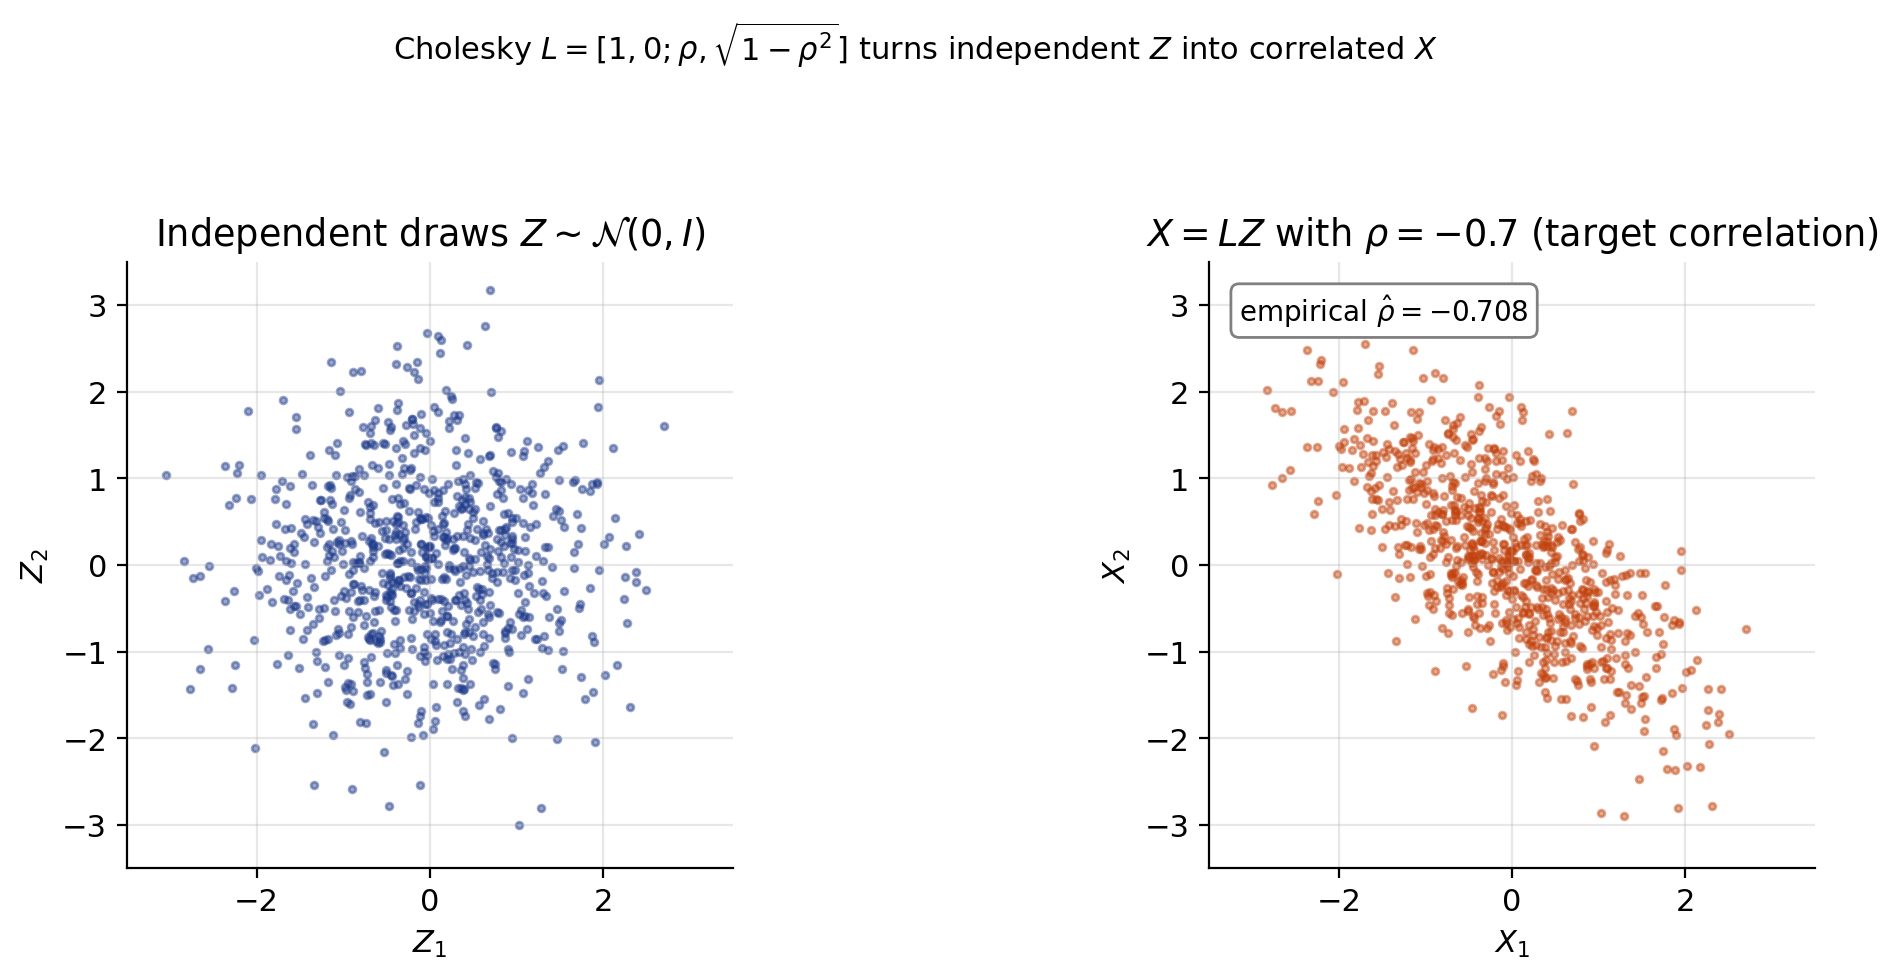
\includegraphics[keepaspectratio]{figures/ch00-cholesky-2d.png}}
\caption{Cholesky \(L=[1,0;\rho,\sqrt{1-\rho^2}]\) turns independent
draws (left) into a correlated cloud at \(\rho=-0.7\) (right) --- the
exact transform applied to \((W^S, W^v)\) in every Heston simulation,
where \(\rho \approx -0.7\) is the empirical SPX-VIX correlation since
2010}
\end{figure}

\[L = \begin{pmatrix} 1 & 0 \\ \rho & \sqrt{1 - \rho^2} \end{pmatrix}. \tag{0.27}\]

The simulation step is then \(dW_1 = \sqrt{dt}\, Z_1\),
\(dW_2 = \sqrt{dt}\, (\rho Z_1 + \sqrt{1-\rho^2}\, Z_2)\) with
independent standard normals \(Z_1, Z_2\).

A 3-asset Cholesky. Take

\[\Sigma = \begin{pmatrix} 1.00 & 0.50 & 0.30 \\ 0.50 & 1.00 & 0.20 \\ 0.30 & 0.20 & 1.00 \end{pmatrix}.\]

Working out the Cholesky entries by the standard recursion
(\(L_{ii}^2 = \Sigma_{ii} - \sum_{k<i} L_{ik}^2\),
\(L_{ji} = (\Sigma_{ji} - \sum_{k<i} L_{jk} L_{ik})/L_{ii}\) for
\(j > i\)):

\[L = \begin{pmatrix} 1.0000 & 0 & 0 \\ 0.5000 & 0.8660 & 0 \\ 0.3000 & 0.0577 & 0.9522 \end{pmatrix}.\]

To sanity check: \(L L'_{22} = 0.5^2 + 0.866^2 = 0.25 + 0.75 = 1.0\) ✓;
\(L L'_{32} = 0.3 \cdot 0.5 + 0.0577 \cdot 0.866 = 0.15 + 0.05 = 0.20\)
✓. \emph{Each Cholesky row builds the new asset's noise as a linear
combination of all prior independent noises plus a fresh shock --- the
variance budget left for the fresh shock is whatever wasn't already
explained by the earlier assets.}

\subsection{0.4.3 Spectral decomposition}\label{spectral-decomposition}

For a symmetric \(A\),

\[A = Q \Lambda Q', \qquad Q \text{ orthogonal}, \;\Lambda = \text{diag}(\lambda_1, \dots, \lambda_n). \tag{0.28}\]

The columns of \(Q\) are orthonormal eigenvectors; the diagonal of
\(\Lambda\) holds the eigenvalues.

\emph{Intuition: every symmetric matrix is a diagonal matrix in the
right basis. The eigenvectors are that basis.}

\textbf{PCA in one line.} If \(\Sigma\) is the covariance matrix of a
return vector and \(\Sigma = Q \Lambda Q'\), then the columns of \(Q\)
are the principal components and the \(\lambda_i\) are the variances of
the returns projected onto each PC. The first PC of the US Treasury
yield curve covariance is roughly flat (level), the second roughly
monotone (slope), the third roughly U-shaped (curvature) --- a classical
and stable result that the term-structure chapters (Ch. 12, 13) lean on.

Concretely, on US Treasury 1Y/2Y/5Y/10Y/30Y daily changes, the first
three eigenvalues typically explain \(\sim 85\% / 10\% / 4\%\) of total
variance. \emph{That decay is what makes 1- and 2-factor short-rate
models (Ch. 12) cover most of the term structure's behaviour with a tiny
parameter count.}

\subsection{0.4.4 Matrix calculus}\label{matrix-calculus}

Two derivatives appear constantly.

\textbf{Linear form.} For \(a, x \in \mathbb{R}^n\),

\[\frac{\partial (a' x)}{\partial x} = a. \tag{0.29}\]

\textbf{Quadratic form.} For symmetric \(A\),

\[\frac{\partial (x' A x)}{\partial x} = 2 A x. \tag{0.30}\]

(For non-symmetric \(A\), the answer is \((A + A')x\); the symmetric
case is what you almost always want.)

These two are sufficient for the first-order conditions in mean-variance
optimisation, regression, and quadratic hedging. \emph{Intuition:
\(a'x\) is linear, so its derivative is the constant slope \(a\);
\(x'Ax\) is the quadratic form, and its derivative is ``twice \(Ax\)''
by the same logic that \(\frac{d}{dx}(ax^2) = 2ax\).}

\begin{figure}
\centering
\pandocbounded{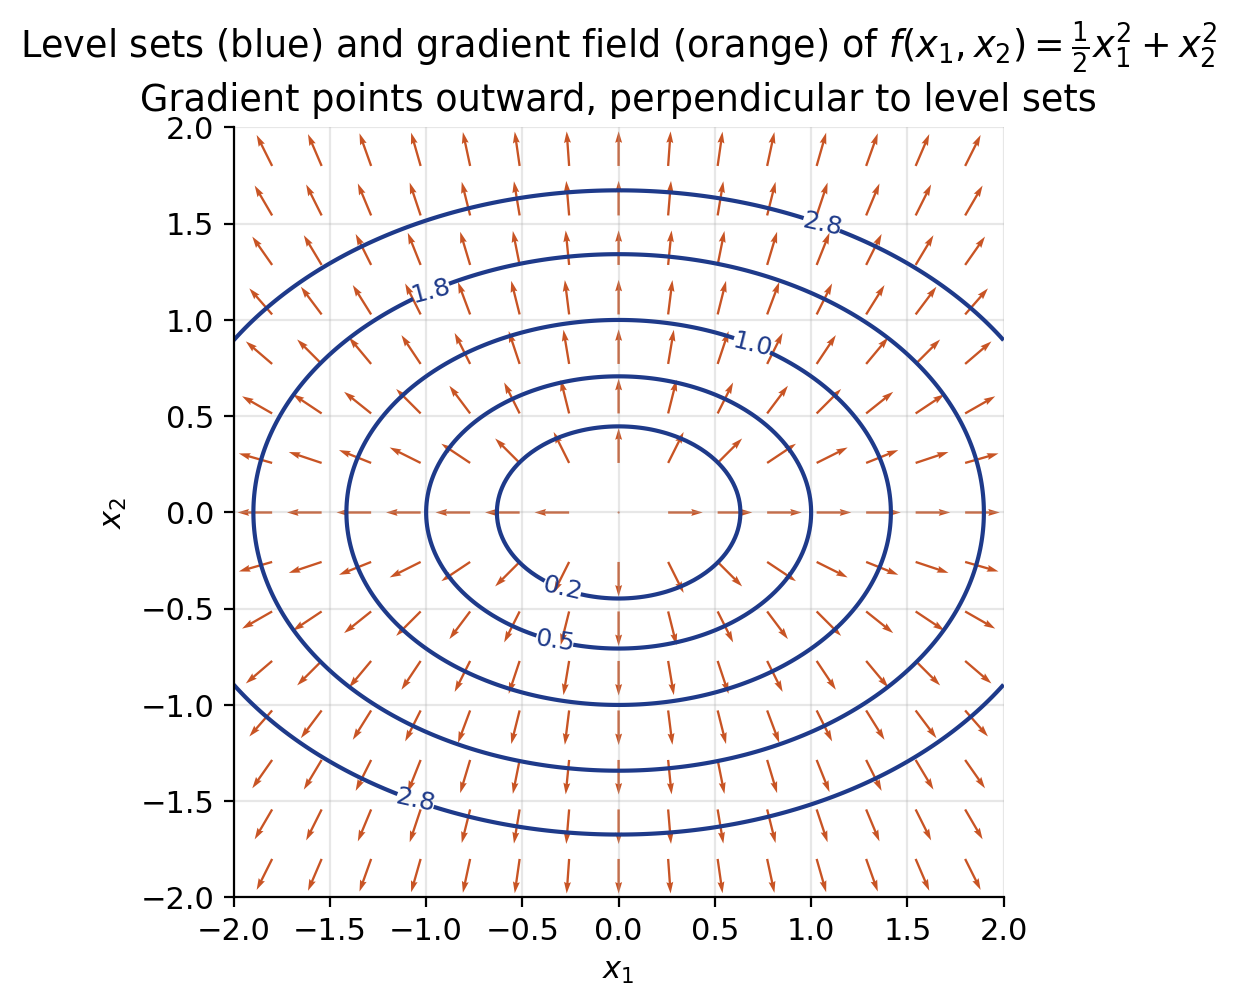
\includegraphics[keepaspectratio]{figures/ch00-grad-levelsets.png}}
\caption{Level sets and gradient field of
\(f(x_1, x_2) = \tfrac{1}{2}x_1^2 + x_2^2\) --- the canonical picture
for steepest-descent calibration of a Heston or short-rate model, where
each level set is an iso-RMSE curve in \((\kappa, \theta)\) space}
\end{figure}

\subsection{0.4.5 Condition number}\label{condition-number}

The \textbf{condition number} of a non-singular \(A\) is

\[\kappa(A) = \frac{\lambda_{\max}(A)}{\lambda_{\min}(A)} \quad \text{(for symmetric PD; in general, the ratio of singular values).} \tag{0.31}\]

It controls how badly small input perturbations distort the solution to
\(Ax = b\):

\[\frac{\|\Delta x\|}{\|x\|} \;\lesssim\; \kappa(A) \,\frac{\|\Delta b\|}{\|b\|}. \tag{0.32}\]

\emph{Rule of thumb: solving \(Ax = b\) in IEEE double precision loses
about \(\log_{10} \kappa(A)\) digits of accuracy. \(\kappa = 10^{12}\)
leaves about 4 digits --- useless for hedging.}

This bites in calibration (Ch. 11): when you solve
\(J' J\, \Delta\theta = J' r\) in Gauss--Newton and the parameters are
nearly degenerate (e.g.~Heston \(v_0\) and \(\theta\) for short
maturities), \(\kappa\) explodes and the update is dominated by noise.
The cure is regularisation (Tikhonov adds \(\lambda I\) to \(J' J\),
lowering \(\kappa\)).

\subsection{0.4.6 A real number}\label{a-real-number-1}

Take a 3-asset equicorrelated correlation matrix with \(\rho = 0.7\):

\[R = \begin{pmatrix} 1 & 0.7 & 0.7 \\ 0.7 & 1 & 0.7 \\ 0.7 & 0.7 & 1 \end{pmatrix}. \tag{0.33}\]

Eigenvalues of an \(n \times n\) equicorrelation matrix with
off-diagonal \(\rho\) are \(1 + (n-1)\rho\) (once, eigenvector
\((1,1,\dots,1)/\sqrt n\)) and \(1 - \rho\) (with multiplicity \(n-1\)).
For \(n=3\), \(\rho = 0.7\):

\[\lambda_1 = 1 + 2 \cdot 0.7 = 2.4, \qquad \lambda_2 = \lambda_3 = 1 - 0.7 = 0.3. \tag{0.34}\]

\emph{Reading the spectrum:} \(\lambda_1 = 2.4\) (out of total trace 3)
is the ``common factor'' --- the equally-weighted portfolio carries 80\%
of the variance. The other 20\% lives in 2-D of long-short directions.

Condition number \(\kappa = 2.4 / 0.3 = 8\) --- well-conditioned.
Cholesky is numerically stable and Monte Carlo will work cleanly. Push
\(\rho\) to \(0.99\): \(\lambda_1 = 2.98\),
\(\lambda_2 = \lambda_3 = 0.01\), \(\kappa = 298\). The matrix is now
nearly singular and Cholesky starts losing 2--3 digits of precision.

\begin{figure}
\centering
\pandocbounded{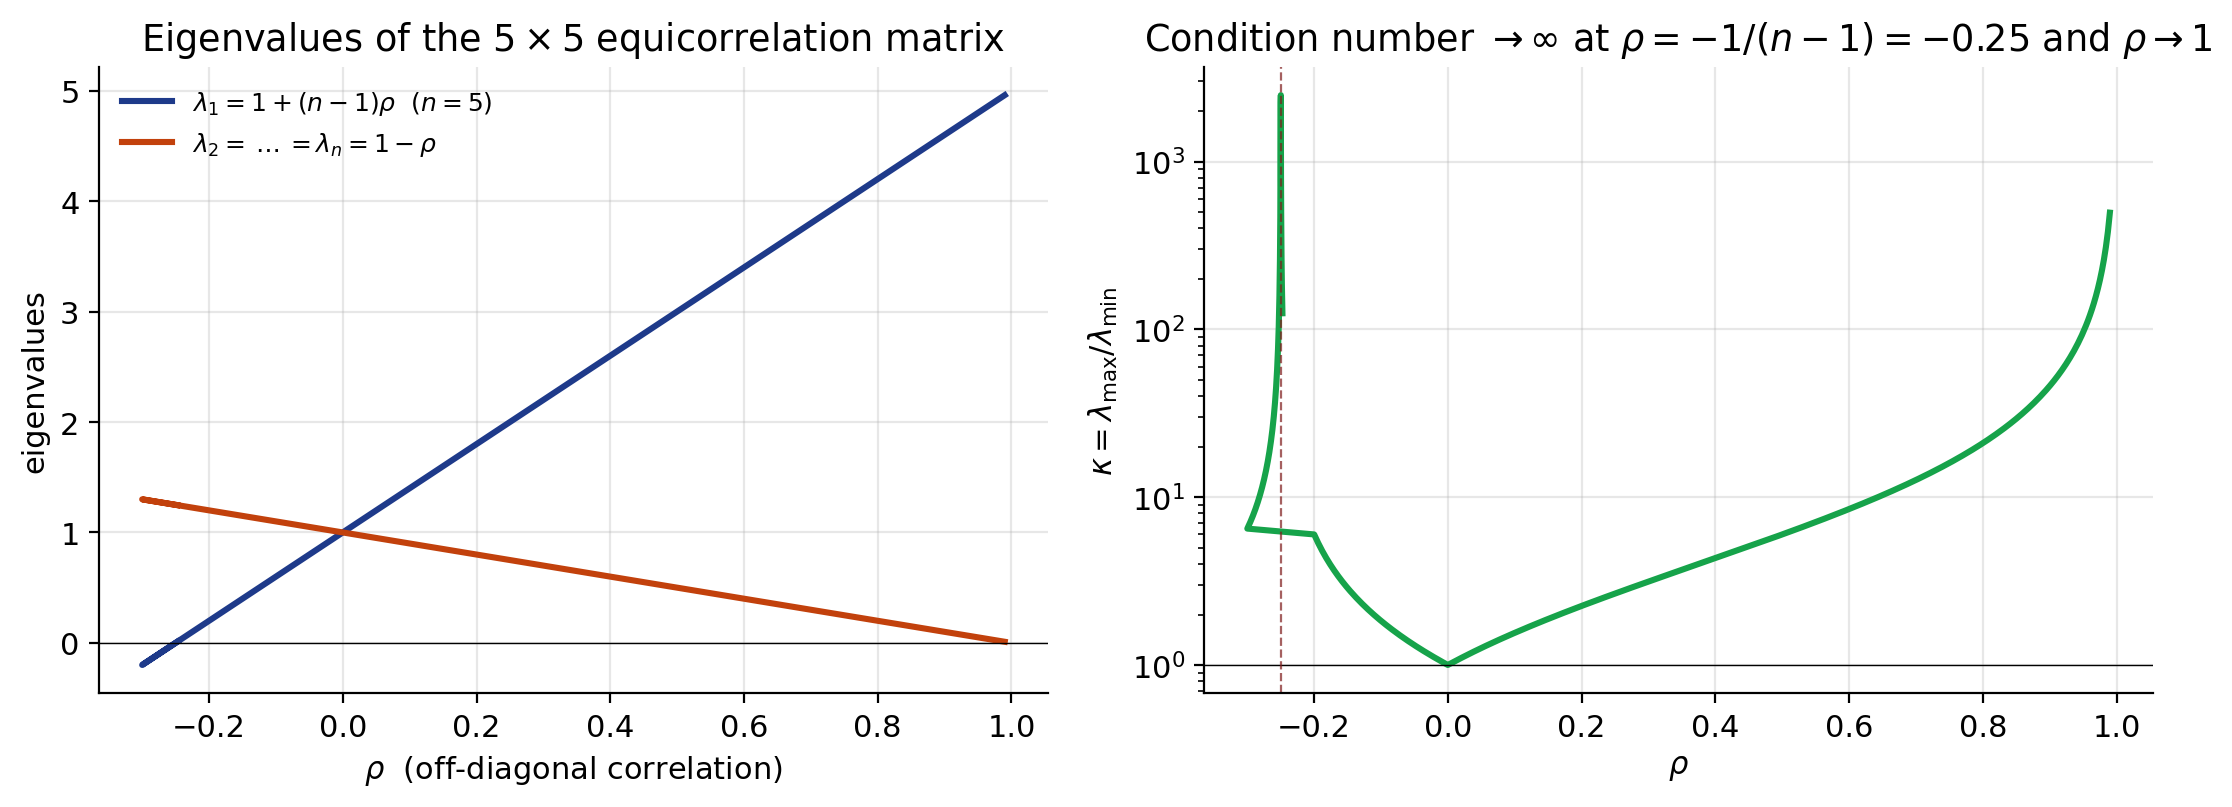
\includegraphics[keepaspectratio]{figures/ch00-pca-equicorr.png}}
\caption{Eigenvalues of the \(5\times 5\) equicorrelation matrix and its
condition number explode as \(\rho \to 1\) --- the failure mode of
mean-variance optimisation on a portfolio of near-identical bond ETFs
(TLT/IEF/SHY all moving together in a rate-rally regime)}
\end{figure}

\subsection{0.4.7 Inverses, pseudo-inverses, and least
squares}\label{inverses-pseudo-inverses-and-least-squares}

The least-squares problem \(\min_\beta \|y - X\beta\|^2\) has normal
equations \(X' X \beta = X' y\), with closed-form solution
\(\hat\beta = (X' X)^{-1} X' y\) when \(X' X\) is invertible.
\emph{Intuition: project \(y\) onto the column space of \(X\);
\(\hat\beta\) is the coordinate vector of that projection in the columns
of \(X\).}

When \(X' X\) is rank-deficient (collinear regressors), the inverse
fails and one uses the \textbf{Moore--Penrose pseudo-inverse} \(X^+\),
equivalently a ridge regression
\(\hat\beta = (X' X + \lambda I)^{-1} X' y\) for some \(\lambda > 0\).
The ridge perturbation lowers the condition number by raising every
eigenvalue by \(\lambda\), at the cost of biasing \(\hat\beta\) toward
zero. \emph{This is the prototype of every regularised calibration in
Ch. 11.}

\subsection{0.4.8 Quadratic optimisation}\label{quadratic-optimisation}

The unconstrained quadratic \(\min_x \tfrac{1}{2} x' A x - b' x\) with
PD \(A\) has stationary point \(A x = b\), i.e.~\(x^\star = A^{-1} b\),
with optimal value \(-\tfrac{1}{2} b' A^{-1} b\). \emph{This is what you
solve in mean-variance portfolio optimisation: \(A\) is the covariance
matrix, \(b\) is the expected-return vector, \(x^\star\) is the
(unconstrained) optimal weight vector.} The fact that \(A\) is PD is
what guarantees the second-order conditions for a minimum.

With a linear equality constraint \(C x = d\) the Lagrangian gives a
closed-form too: a \(2 \times 2\) block solve. Mean-variance with a
budget constraint \(\mathbf{1}'x = 1\) is exactly this case.

\subsection{0.4.9 Eigenvalues of common parametric
families}\label{eigenvalues-of-common-parametric-families}

\textbf{Equicorrelation matrix.} \(R_{ij} = \rho\) off-diagonal, 1 on
the diagonal: eigenvalues \(1 + (n-1)\rho\) (once) and \(1 - \rho\)
(with multiplicity \(n-1\)). Used in (0.34) and seen any time a model
assumes a single common factor.

\textbf{Tridiagonal Toeplitz (AR(1)-style).} \(A_{ii} = a\),
\(A_{i,i\pm 1} = b\): eigenvalues \(a + 2b \cos(k\pi/(n+1))\) for
\(k = 1, \dots, n\). \emph{Used by every finite-difference scheme for
the BS PDE (Ch. 6) --- those grids generate exactly this matrix
structure, and the cosine eigenvalues control numerical stability.}

Knowing these spectra lets you read off condition numbers and stability
limits without ever calling an eigensolver.

\begin{center}\rule{0.5\linewidth}{0.5pt}\end{center}

\section{§0.5 Calculus and ODE
Refresher}\label{calculus-and-ode-refresher}

You should not need this section. It is here as a fallback so the rest
of the guide has nothing left to assume.

\subsection{0.5.0 What you should already
know}\label{what-you-should-already-know}

Differentiation, integration, the fundamental theorem of calculus,
existence/uniqueness for Lipschitz ODEs. One reminder: \(f\) is
\textbf{Lipschitz} with constant \(L\) if
\(|f(x) - f(y)| \leq L|x - y|\), and Picard--Lindelöf says Lipschitz RHS
gives unique local ODE solutions. \emph{Every SDE coefficient in this
guide will be Lipschitz, so you can stop worrying about it.}

\subsection{0.5.1 Taylor expansion}\label{taylor-expansion}

For \(f\) smooth at \(x\),

\[f(x + h) = f(x) + f'(x) h + \tfrac{1}{2} f''(x) h^2 + \tfrac{1}{6} f'''(x) h^3 + O(h^4). \tag{0.35}\]

Multivariate version with \(h \in \mathbb{R}^n\):

\[f(x + h) = f(x) + (\nabla f)' h + \tfrac{1}{2} h' (\nabla^2 f) h + O(\|h\|^3). \tag{0.36}\]

This is the deterministic counterpart of Itô's lemma (Ch. 3). In
ordinary calculus, the second-order term \(\tfrac{1}{2} f''(x) h^2\)
vanishes as \(h \to 0\) because it is \(O(h^2)\). \emph{In Itô calculus,
\(h\) is a Brownian increment with \(\mathrm{Var}(h) \sim h\) rather
than \(h^2\), so the second-order term contributes a \(O(dt)\) piece
that does not vanish --- that is the entire reason Itô differs from the
chain rule.}

The same point in option-pricing language: a delta hedge captures the
first-order term \(f'(x) h\). The remaining error per timestep is the
gamma term \(\tfrac{1}{2} f''(x) h^2\), and over a hedging interval
\(dt\), that error has expected size
\(\tfrac{1}{2} \Gamma \sigma^2 S^2\, dt\). \emph{The \(\sigma^2/2\) from
§0.2 reappears as the per-unit-time cost of being short gamma ---
Jensen's gap is the gamma P\&L of an unhedged convex position.}

\begin{figure}
\centering
\pandocbounded{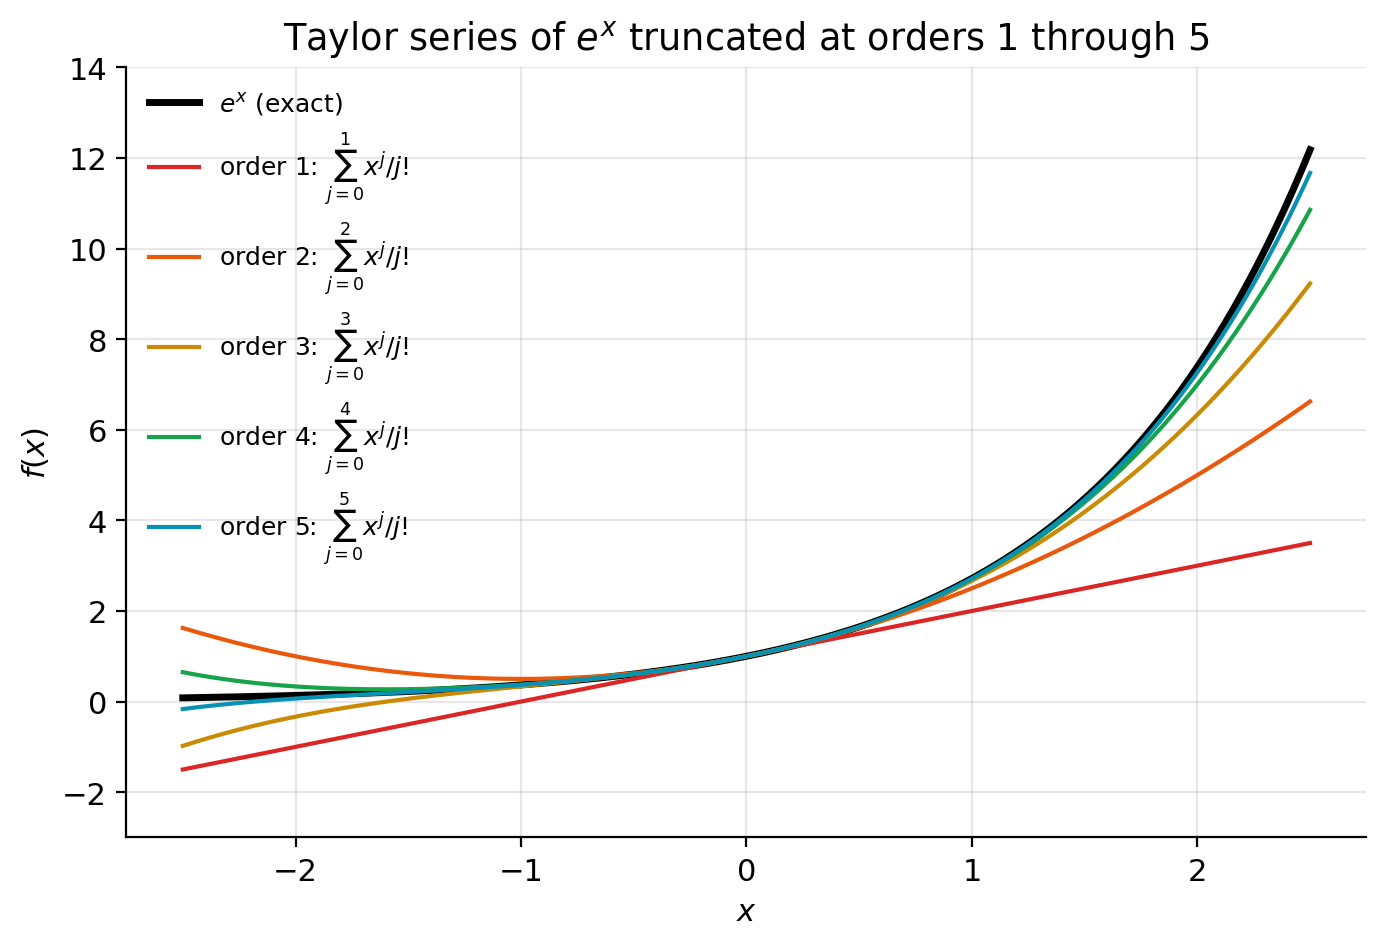
\includegraphics[keepaspectratio]{figures/ch00-taylor-exp.png}}
\caption{Taylor truncations of \(e^x\) at orders 1-5 against the exact
curve. Each added order kills another factor of \(h\) in the residual
--- the same convergence underlying every Itô-Taylor expansion of a
smooth payoff used for Greeks, where delta is the order-1 piece and
gamma the order-2 piece}
\end{figure}

Sanity check with \(f(x) = e^x\) at \(x = 0\), \(h = 0.1\):

{\def\LTcaptype{none} % do not increment counter
\begin{longtable}[]{@{}lll@{}}
\toprule\noalign{}
Order & Approximation & Value \\
\midrule\noalign{}
\endhead
\bottomrule\noalign{}
\endlastfoot
1st & \(1 + 0.1\) & \(1.10000\) \\
2nd & \(1 + 0.1 + \tfrac{0.01}{2}\) & \(1.10500\) \\
3rd & \(\dots + \tfrac{0.001}{6}\) & \(1.10517\) \\
Exact & \(e^{0.1}\) & \(1.10517\) \\
\end{longtable}
}

Each order kills another factor of \(h\) in the residual; that is the
meaning of \(O(h^k)\).

\subsection{0.5.2 Chain rule,
multivariate}\label{chain-rule-multivariate}

For \(f : \mathbb{R}^n \to \mathbb{R}\) and
\(g : \mathbb{R} \to \mathbb{R}^n\),

\[\frac{d}{dt} f(g(t)) = (\nabla f)(g(t)) \cdot g'(t) = \sum_i \frac{\partial f}{\partial x_i} \frac{dg_i}{dt}. \tag{0.37}\]

For change of variables in integration with \(u = \phi(x)\),

\[\int f(\phi(x)) |\phi'(x)|\, dx = \int f(u)\, du. \tag{0.38}\]

The Jacobian determinant generalises this to multidimensions and is the
root of the change-of-density formulae used in Girsanov (Ch. 5).

In the multivariate case with \(u = \phi(x)\) for
\(\phi: \mathbb{R}^n \to \mathbb{R}^n\) differentiable and bijective on
the domain,

\[\int f(\phi(x)) |\det J_\phi(x)|\, dx = \int f(u)\, du, \qquad J_\phi = \left(\frac{\partial \phi_i}{\partial x_j}\right). \tag{0.39}\]

\emph{Intuition: the determinant of the Jacobian is the local volume
scaling of the change of variables; it is what makes the integrand
densities consistent.} The Radon--Nikodym derivative
\(d\mathbb{Q}/d\mathbb{P}\) in change of measure is the
infinite-dimensional analogue: a ``Jacobian'' between two probability
laws on path space.

For densities: if \(X\) has density \(f_X\) and \(Y = g(X)\) for
monotone differentiable \(g\),

\[f_Y(y) = f_X(g^{-1}(y)) \cdot \left|\frac{d g^{-1}(y)}{dy}\right|.\]

Apply this to \(Y = e^X\) with \(X \sim N(\mu, \sigma^2)\) and you get
the log-normal density --- the foundational distribution of asset prices
in this guide. \emph{The factor \(1/y\) in the log-normal density is
exactly the Jacobian of \(g^{-1} = \log\).}

\subsection{0.5.3 Separable ODE}\label{separable-ode}

The single most-used ODE in the guide,

\[\frac{dy}{dt} = a(t) y \;\;\Longleftrightarrow\;\; \frac{dy}{y} = a(t)\, dt \;\;\Longleftrightarrow\;\; \log y(t) = \log y(0) + \int_0^t a(s)\, ds. \tag{0.40}\]

Canonical case \(a(t) \equiv \mu\): \(y(t) = y(0) e^{\mu t}\) ---
exponential growth.

The deterministic version \(dS/S = \mu\, dt\) gives
\(S_t = S_0 e^{\mu t}\). The stochastic version
\(dS/S = \mu\, dt + \sigma\, dW\) gives the GBM solution
\(S_t = S_0 \exp[(\mu - \tfrac{1}{2}\sigma^2)t + \sigma W_t]\)
(cf.~(0.13)) --- same separability, plus the Itô correction.

\subsection{0.5.4 Linear first-order ODE and the integrating
factor}\label{linear-first-order-ode-and-the-integrating-factor}

The linear ODE

\[y'(t) + p(t)\, y(t) = q(t) \tag{0.41}\]

is solved by multiplying through by the \textbf{integrating factor}
\(\mu(t) = \exp\!\left(\int p(s)\, ds\right)\). The left-hand side then
becomes a clean derivative:

\[\frac{d}{dt}\!\left[\mu(t)\, y(t)\right] = \mu(t)\, q(t). \tag{0.42}\]

Integrate and divide by \(\mu(t)\):

\[y(t) = \mu(t)^{-1} \!\left[ y(0) + \int_0^t \mu(s)\, q(s)\, ds \right]. \tag{0.43}\]

\emph{Intuition: the integrating factor \(\mu(t)\) is constructed
precisely so that \(\mu \cdot (y' + p y) = (\mu y)'\) --- it cancels the
operator \(\frac{d}{dt} + p(t)\) into a clean total derivative.} This is
one of the few solution recipes in classical ODEs that generalises
immediately to SDEs.

\subsection{0.5.5 Vasicek as a linear ODE plus
noise}\label{vasicek-as-a-linear-ode-plus-noise}

The Vasicek short-rate model (Ch. 12),

\[dr_t = \kappa(\theta - r_t)\, dt + \sigma\, dW_t, \tag{0.44}\]

has a closed-form solution that looks intimidating until you notice it
is \emph{exactly} the linear-ODE structure of (0.37) with
\(p(t) \equiv \kappa\) and \(q(t) \equiv \kappa \theta\), plus a noise
term \(\sigma\, dW\).

Apply the integrating factor \(\mu(t) = e^{\kappa t}\). The
mean-reverting deterministic ODE \(dr/dt + \kappa r = \kappa \theta\)
has solution

\[r_t^{\text{det}} = e^{-\kappa t} r_0 + \theta\,(1 - e^{-\kappa t}). \tag{0.45}\]

Adding the stochastic forcing using the same integrating factor,

\[r_t = e^{-\kappa t} r_0 + \theta\,(1 - e^{-\kappa t}) + \sigma \int_0^t e^{-\kappa(t - s)}\, dW_s. \tag{0.46}\]

\emph{Reading: the deterministic part is the linear ODE solution; the
stochastic part is the same integrating-factor trick applied to the
\(dW\) noise. The factor \(e^{-\kappa(t-s)}\) in the stochastic integral
is the Green's function of the linear operator --- old shocks decay
exponentially with mean-reversion rate \(\kappa\).}

The integral term is Gaussian with mean zero and variance
\(\frac{\sigma^2}{2\kappa}(1 - e^{-2\kappa t})\) (use the Itô isometry,
Ch. 3). So \(r_t\) is Gaussian, mean-reverting, with long-run
distribution \(N(\theta, \sigma^2 / (2\kappa))\).

This is the working pattern for \emph{every} Ornstein--Uhlenbeck-style
process you meet in this guide: identify the linear ODE skeleton, write
down the integrating factor, add the stochastic forcing.

Take \(\kappa = 0.5\) (per year), \(\theta = 4\%\), \(\sigma = 1\%\),
\(r_0 = 2\%\).

\begin{itemize}
\tightlist
\item
  Mean reversion half-life: \(\log 2 / \kappa = 1.39\) years --- the gap
  to the long-run mean halves every 17 months.
\item
  Long-run mean: \(\theta = 4\%\).
\item
  Long-run standard deviation:
  \(\sigma / \sqrt{2\kappa} = 0.01 / 1 = 1.0\%\).
\item
  Time-1 distribution:
  \(r_1 \sim N\!\left(e^{-0.5}\cdot 0.02 + 0.04 \cdot (1 - e^{-0.5}),\; \tfrac{0.01^2}{1}(1 - e^{-1})\right) = N(0.0279,\; 0.0079^2)\).
\end{itemize}

So a year out, the rate is centred at 2.79\% with a 79bp one-sigma ---
it has crawled three-quarters of the way back to \(\theta\) and acquired
most of its long-run dispersion. \emph{The two timescales --- mean
reversion and noise build-up --- are completely controlled by
\(\kappa\). The half-life is \(\log 2 / \kappa\); the variance saturates
at \(\sigma^2 / (2\kappa)\). Vasicek has only three knobs and they each
do exactly one thing.}

\subsection{0.5.6 PDE pattern
recognition}\label{pde-pattern-recognition}

Four PDE archetypes recur throughout the guide. Recognising them on
sight saves you solving from scratch.

{\def\LTcaptype{none} % do not increment counter
\begin{longtable}[]{@{}
  >{\raggedright\arraybackslash}p{(\linewidth - 4\tabcolsep) * \real{0.3333}}
  >{\raggedright\arraybackslash}p{(\linewidth - 4\tabcolsep) * \real{0.3333}}
  >{\raggedright\arraybackslash}p{(\linewidth - 4\tabcolsep) * \real{0.3333}}@{}}
\toprule\noalign{}
\begin{minipage}[b]{\linewidth}\raggedright
Archetype
\end{minipage} & \begin{minipage}[b]{\linewidth}\raggedright
Equation form
\end{minipage} & \begin{minipage}[b]{\linewidth}\raggedright
Where it appears
\end{minipage} \\
\midrule\noalign{}
\endhead
\bottomrule\noalign{}
\endlastfoot
Heat / diffusion & \(u_t = \tfrac{1}{2}\sigma^2 u_{xx}\) & BS after
change of variable (Ch. 5--6) \\
Drift-diffusion (Kolmogorov backward) &
\(u_t + \mu u_x + \tfrac{1}{2}\sigma^2 u_{xx} = 0\) & Feynman--Kac (Ch.
4) \\
Drift-diffusion with discounting &
\(u_t + \mu u_x + \tfrac{1}{2}\sigma^2 u_{xx} - r u = 0\) & BS PDE (Ch.
6) \\
Two-factor diffusion &
\(u_t + \mathcal{L}_S u + \mathcal{L}_v u + \rho \sigma_S \alpha\,u_{Sv} - r u = 0\)
& Heston (Ch. 10): \(\alpha\) is vol-of-vol \\
\end{longtable}
}

\emph{Each is a parabolic PDE; each has a Feynman--Kac stochastic
representation; each can be solved by characteristics, Fourier methods,
finite differences, or Monte Carlo. The choice of method is a numerical
question, not a modelling one.}

\begin{center}\rule{0.5\linewidth}{0.5pt}\end{center}

\section{§0.6 Reading the Rest of This
Guide}\label{reading-the-rest-of-this-guide}

This chapter is a reference. Read it once carefully, then revisit when
later chapters cite a specific section. The table below shows which
prerequisite each chapter actually leans on.

{\def\LTcaptype{none} % do not increment counter
\begin{longtable}[]{@{}
  >{\raggedright\arraybackslash}p{(\linewidth - 4\tabcolsep) * \real{0.3333}}
  >{\raggedright\arraybackslash}p{(\linewidth - 4\tabcolsep) * \real{0.3333}}
  >{\raggedright\arraybackslash}p{(\linewidth - 4\tabcolsep) * \real{0.3333}}@{}}
\toprule\noalign{}
\begin{minipage}[b]{\linewidth}\raggedright
Chapter
\end{minipage} & \begin{minipage}[b]{\linewidth}\raggedright
Topic
\end{minipage} & \begin{minipage}[b]{\linewidth}\raggedright
Prerequisites from §0
\end{minipage} \\
\midrule\noalign{}
\endhead
\bottomrule\noalign{}
\endlastfoot
Ch. 1 & One-Period Binomial & §0.1.1 (probability spaces), §0.1.2
(conditional expectation) --- light \\
Ch. 2 & Multi-Period Binomial \& FTAP & §0.1.2 (tower), §0.3.2
(martingales), §0.3.5 (optional sampling) \\
Ch. 3 & Stochastic Calculus Primer & §0.1 throughout, §0.3 throughout,
§0.5.1 (Taylor --- Itô is the stochastic Taylor) \\
Ch. 4 & Feynman--Kac & §0.3.3 (Markov), §0.5.4 (linear ODEs) --- PDEs
are ODEs in time with elliptic operator in space \\
Ch. 5 & Measure Changes \& Girsanov & §0.1.4 (MGF --- the Radon--Nikodym
derivative is a normalised exponential MGF), §0.3.2 (martingales) \\
Ch. 6 & Dynamic Hedging (BS PDE) & §0.5.1 (Taylor), §0.2 (the
\(\sigma^2/2\) in the BS PDE is Jensen) \\
Ch. 7 & Greeks & §0.4.4 (matrix calculus for cross-Greeks), §0.2 (vol
convexity = Vega convexity = Jensen) \\
Ch. 8 & Forwards/Futures/Black PDE & §0.2 (convexity adjustment for
futures vs forwards is Jensen), §0.5.4 (linear ODE for the forward) \\
Ch. 9 & Monte Carlo & §0.1.5 (modes of convergence), §0.4.2 (Cholesky
for correlated paths) \\
Ch. 10 & Heston & §0.4.2 (Cholesky for the asset-vol correlation),
§0.1.4 (characteristic functions because Heston has no MGF for
\(S_T\)) \\
Ch. 11 & Calibration & §0.4.5 (condition number --- calibration is an
ill-posed inverse problem), §0.4.4 (gradient of squared error) \\
Ch. 12 & Short-Rate Models & §0.5.5 (Vasicek as integrating factor),
§0.3.2 (martingale measure for the bank account) \\
Ch. 13 & Rate-Derivative Applications & §0.5.4 (forward rates as ODE
solutions), §0.3.6 (Doob--Meyer for the convexity adjustment) \\
Ch. 14 & Caps/Floors/Swaptions & §0.2 (Black's formula is GBM under the
forward measure --- full Jensen content) \\
Ch. 15 & Risk Measures (capstone) & §0.1.5 (convergence for empirical
VaR), §0.1.6 (Borel--Cantelli for tail-event frequency) \\
\end{longtable}
}

The single highest-traffic section is §0.2. The second is §0.3.2
(martingales). The third is §0.4.2 (Cholesky). If you read those three
carefully you will follow 80\% of the guide without ever flipping back
here.

What is \emph{not} here: Itô's lemma, stochastic integration, and the
Itô isometry are deferred to Ch. 3; the BS PDE and Feynman--Kac to Ch. 4
and 6; change of measure to Ch. 5; numerical methods to their respective
application chapters. Only prerequisites live here.

When a later chapter writes ``by Jensen'' or ``by the tower property''
without further comment, it refers to this chapter.

\subsection{0.6.1 A cross-reference
walkthrough}\label{a-cross-reference-walkthrough}

The chain of refresher dependencies invoked in one page of the Ch. 6 BS
PDE derivation:

\begin{enumerate}
\def\labelenumi{\arabic{enumi}.}
\tightlist
\item
  Take a smooth function \(V(t, S)\) of the asset price \(S_t\)
  following GBM, \(dS = \mu S\, dt + \sigma S\, dW\).
\item
  Apply Itô's lemma (Ch. 3, prefigured in §0.3.8 here) to get
  \[dV = \left(V_t + \mu S V_S + \tfrac{1}{2}\sigma^2 S^2 V_{SS}\right) dt + \sigma S V_S\, dW.\]
\item
  Note the second-order term \(\tfrac{1}{2}\sigma^2 S^2 V_{SS}\) is the
  \textbf{Jensen gap of \(V\) in \(S\)}, weighted by the instantaneous
  variance --- that is §0.2.7 made dynamic.
\item
  Form a self-financing portfolio long one option, short \(V_S\) shares;
  the \(dW\) terms cancel by construction (delta hedging).
\item
  The remaining drift must equal the riskless rate (no arbitrage), so
  \(V_t + \tfrac{1}{2}\sigma^2 S^2 V_{SS} = rV - r S V_S\) --- the BS
  PDE.
\item
  The PDE is solved either by Feynman--Kac (Ch. 4, using §0.3.3 Markov),
  or by transforming to the heat equation (Ch. 5, change of variables
  from §0.5.2).
\item
  The resulting price formula is a Gaussian expectation under
  \(\mathbb{Q}\) (Ch. 5, using §0.1.4 MGF and §0.3.2 martingales).
\end{enumerate}

That single page leans on (in order) §0.5.1, §0.3.8, §0.2.7, §0.3.2,
§0.3.3, §0.5.2, §0.1.4, §0.1.2 --- eight sections, mostly without
explicit citation. \emph{That is the density at which this chapter is
consumed.}

\subsection{0.6.2 What to memorise}\label{what-to-memorise}

Five facts to keep in working memory.

\begin{enumerate}
\def\labelenumi{\arabic{enumi}.}
\tightlist
\item
  \textbf{Tower property}
  \(\mathbb{E}[\mathbb{E}[X \mid \mathcal{G}] \mid \mathcal{H}] = \mathbb{E}[X \mid \mathcal{H}]\)
  --- every change-of-measure or change-of-numéraire argument hinges on
  this.
\item
  \textbf{Jensen gap for log-normal} \(= \sigma^2 / 2\) per unit time.
  The same gap appears as Itô correction, GBM log-drift, vol drag, and
  BS gamma P\&L.
\item
  \textbf{Martingale property under \(\mathbb{Q}\)} of discounted price
  processes. This is the modern definition of ``no arbitrage'' and is
  what makes pricing work.
\item
  \textbf{Cholesky of \(\Sigma\)} is the recipe for correlated Brownian
  simulation. Memorise the 2-D form
  \(L = (1, 0; \rho, \sqrt{1-\rho^2})\).
\item
  \textbf{Linear ODE solved by integrating factor.} Vasicek and every
  short-rate model with a closed form is built on this single trick.
\end{enumerate}

Everything else can be looked up. These five recur often enough that not
having them at fingertip cost is a tax on every chapter.

Turn to Ch. 1 for the binomial model, where the arbitrage-pricing
framework is built from scratch before the continuous-time machinery is
unleashed in Ch. 3.

\begin{center}\rule{0.5\linewidth}{0.5pt}\end{center}

\emph{End of Chapter 0.}

\newpage

\chapter{Chapter 1 --- One-Period Binomial: No-Arbitrage and
Replication}\label{chapter-1-one-period-binomial-no-arbitrage-and-replication}

This chapter develops arbitrage-free pricing in the simplest possible
model: a single risky asset with two future values, observed over one
time step. We introduce a numeraire bond, define arbitrage, and show
that the absence of arbitrage forces a unique synthetic probability
measure under which discounted asset prices are martingales. Every
continuous-time pricing formula in the rest of the book ---
Black--Scholes, Heston, HJM --- is a limiting case of what is derived in
the next few pages.

\begin{quote}
Narrative spine. A derivative's price is the cost of the portfolio that
replicates it, computed as a discounted expectation under a measure that
makes traded assets martingales. The binomial model isolates this idea
cleanly with no stochastic calculus, no measure-theoretic probability,
and no Itô's lemma --- yet every conceptual ingredient of the
continuous-time theory appears in finite-dimensional form. We do not
invoke utility theory or preferences: replication forces the price to
depend only on hedging cost. Indifference pricing for non-replicable
claims is treated separately in the appendix.
\end{quote}

\begin{center}\rule{0.5\linewidth}{0.5pt}\end{center}

\section{1. The One-Period Binomial
Tree}\label{the-one-period-binomial-tree}

Consider a single risky asset \(A\) observed at two dates \(t = 0\) and
\(t = 1\). At \(t=1\) the price takes one of two values, \(A_u\) (up) or
\(A_d\) (down), with real-world up-probability

\[p \in (0,1). \tag{1.1}\]

Strict positivity (\(p \in (0,1)\), not \([0,1]\)) keeps both states
genuinely reachable under \(\mathbb{P}\) and forces any equivalent
martingale measure \(\mathbb{Q}\) to assign positive weight to both
branches as well --- without it the pricing theory collapses on
equivalence grounds.

\begin{figure}
\centering
\pandocbounded{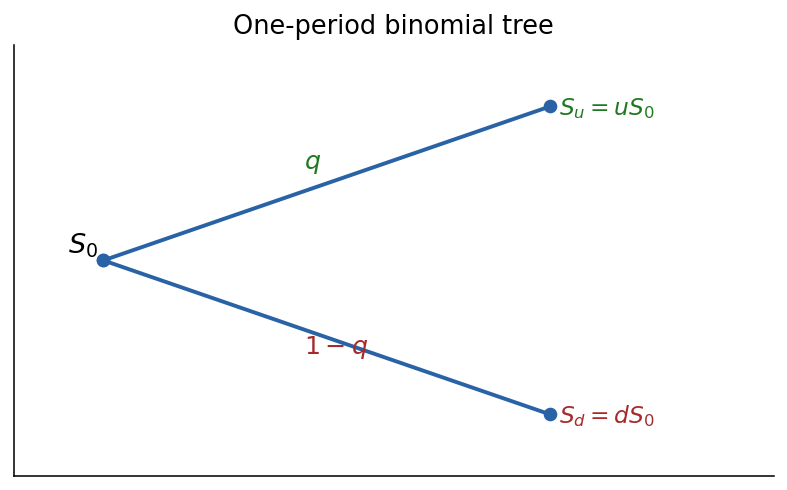
\includegraphics[keepaspectratio]{figures/ch01-tree.png}}
\caption{One-period binomial tree}
\end{figure}

\emph{One-period binomial tree.}

The (random) time-1 price can be written as a function of a Bernoulli
indicator \(x_1 \in \{1, 0\}\):

\[A_1 = A_u\, x_1 + A_d\,(1 - x_1), \qquad x_1 = \begin{cases} 1 & \text{w.p. } p \\ 0 & \text{w.p. } 1-p. \end{cases} \tag{1.2}\]

A single random coordinate \(x_1\) generates the whole filtration
\(\mathcal{F}_1\) --- one source of randomness, one degree of freedom to
hedge it with. That dimension match (one coin, two assets) is exactly
what later delivers a \emph{unique} risk-neutral measure. Replace
\(x_1\) with a three-valued random variable and the count breaks: three
payoffs to match, two assets, generically no replication --- the
simplest incomplete market.

A naïve ``discounted expectation under \(\mathbb{P}\)'' guess for the
price is

\[A_0 \;=\; \frac{p\,A_u + (1-p)\,A_d}{1 + r}, \qquad A_0 \in (A_d, A_u), \tag{1.3}\]

with \(r\) the one-period risk-free rate. (1.3) is \emph{not} a pricing
rule --- \(\mathbb{P}\) does not price, only a risk-neutral measure
\(\mathbb{Q}\) does. (1.3) implicitly assumes \(A\) earns the risk-free
rate, but a risky asset earns \(r\) plus a premium; that premium is what
distinguishes \(\mathbb{P}\) from \(\mathbb{Q}\).

\subsection{1.1 Two numerical examples --- why expected value is not
enough}\label{two-numerical-examples-why-expected-value-is-not-enough}

Two symmetric lotteries with identical \(\mathbb{P}\)-expectation but
very different ``felt'' risk:

\[p = \tfrac{1}{2}, \qquad A_u = 100, \qquad A_d = -100. \tag{1.4}\]

\[p = \tfrac{1}{2}, \qquad A_u = 10^{6}, \qquad A_d = -10^{6}. \tag{1.5}\]

Both have zero expected payoff; no one would price them the same --- the
second is existentially ruinous. Expected value alone cannot price for a
risk-averse agent. The miracle of no-arbitrage pricing (§2) is that
risk-aversion cancels out as soon as the payoff is replicable.

\subsection{Case study: Buffett's long-dated SPX put sale
(2006--2026)}\label{case-study-buffetts-long-dated-spx-put-sale-20062026}

\emph{Berkshire Hathaway sold \(\sim\) \$36B notional of European-style
put options on four global equity indices (S\&P 500, FTSE, Euro Stoxx
50, Nikkei) between 2004 and 2008, collecting roughly \$4.5B in premium
upfront and contracting to pay only at maturities clustering between
2018 and 2028. Buffett famously called the Black-Scholes price of these
contracts ``Alice in Wonderland.'' By the time the last expirations
rolled off in 2026, every index sat well above its 2006-era strikes and
the entire \$36B notional expired worthless --- Berkshire kept the full
\$4.5B premium plus 20 years of float.}

\textbf{Context.} The contracts were European, deeply out-of-the-money
(struck close to the 2006--2008 spot levels), and could not be exercised
before maturity --- the only cashflow risk was the terminal payoff
\(\max(K - S_T, 0)\) at expiries 15--20 years out. Counterparties
(mostly investment banks repackaging structured-product downside
protection) wanted a long-vol, long-equity-tail hedge; only an entity
with a permanent capital base could plausibly \emph{write} it without
onerous collateral terms. Buffett's pitch was simple: over 20 years, the
indices in question had never been negative once you included dividends,
and Berkshire's \(\mathbb{P}\)-view assigned essentially zero
probability to the strikes being breached at expiry. Realised history
validated him: over 2006--2026, the S\&P 500 went from \(\sim\) 1280 in
March 2006 to \(\sim\) 5300 in May 2026, a 4\(\times\) cumulative move;
the Nikkei staged a similar (delayed) recovery; FTSE and Euro Stoxx 50
both finished above their 2006 marks. Every option ended worthless.

\textbf{Math mapping.} Read this through the one-period machinery of §1.
Berkshire's \(\mathbb{P}\)-expected payoff was deeply negative (i.e.~the
option had near-zero \(\mathbb{P}\)-expected loss to the writer); the
bank counterparties' \(\mathbb{Q}\)-expected payoff, computed with a
Black-Scholes vol surface implying \(\sim\) 20\% vol over a 20-year
horizon, was substantial --- fat enough to justify quoting the contract
at a multi-billion dollar premium. The disagreement is not mathematical
error on either side; it is the formal one-period observation that the
\emph{risk-neutral} price (2.2) requires a \emph{replicating hedge}, and
at 20-year tenors there is no liquid hedge instrument --- no traded
20-year SPX option, no 20-year variance swap, nothing to short against.
The synthetic \(\mathbb{Q}\) in §2 is constructed from prices of
\emph{traded} hedge instruments at the relevant horizon; without those,
the formal \(\mathbb{Q}\)-price is academic and the actual transaction
price gets pulled back toward the writer's \(\mathbb{P}\)-view plus a
risk-premium charge for warehousing the un-hedgeable risk. Buffett's
edge was that Berkshire's capital base (then \$120B, now well over
\$300B) made the firm \emph{effectively risk-neutral} at this scale ---
the marginal utility of a \$36B tail loss, conditional on it occurring
inside a portfolio that size, was approximately linear, so Berkshire
could quote a price close to its \(\mathbb{P}\)-expected loss rather
than a distorted utility-of-loss price. The premium it collected was the
variance risk premium that the broader market could not absorb for lack
of hedge counterparties.

\textbf{Lesson.} Three takeaways for the new hire. First, the §1
separation of ``preference-free pricing where replication is possible''
from ``preference-driven pricing where it is not'' is not a textbook
nicety --- it is the entire economic reason this trade existed. The bank
counterparties had no choice but to lay off the risk somewhere;
Berkshire was the only entity sized to take it without requiring a
hedge. Second, \(\mathbb{Q}\)-pricing is a lever, not a law: when no
hedge instrument exists at your horizon, the \emph{formal}
\(\mathbb{Q}\)-price loses its no-arb teeth and the realised price
collapses to ``what does the marginal warehouser charge to hold this
risk on its book.'' Third, the trade is a clean illustration of the
variance risk premium: implied vol over 20-year horizons is structurally
higher than realised vol because there is no efficient mechanism to
short it; the writers of long-dated puts capture that premium and absorb
the (rare, fat-tailed) downside in exchange. Berkshire kept \$4.5B + 20
years of float because its capital base was large enough to make the
un-hedgeable risk warehousable on its balance sheet at a price the
market was willing to pay.

\begin{center}\rule{0.5\linewidth}{0.5pt}\end{center}

\section{2. Two-Asset Model and
Arbitrage}\label{two-asset-model-and-arbitrage}

Introduce a second asset and argue purely from the absence of arbitrage.
The result is a formula that looks like an expected value --- under a
synthetic measure \(\mathbb{Q}\) that prices every replicable claim
correctly.

Two assets at \(t=0, 1\): risky \(A\) and numeraire \(B\), both driven
by the \emph{same} Bernoulli coin. In the bond case
\(B_u = B_d = B_0(1+r)\); the general case allows \(B\) its own leaves:

\begin{figure}
\centering
\pandocbounded{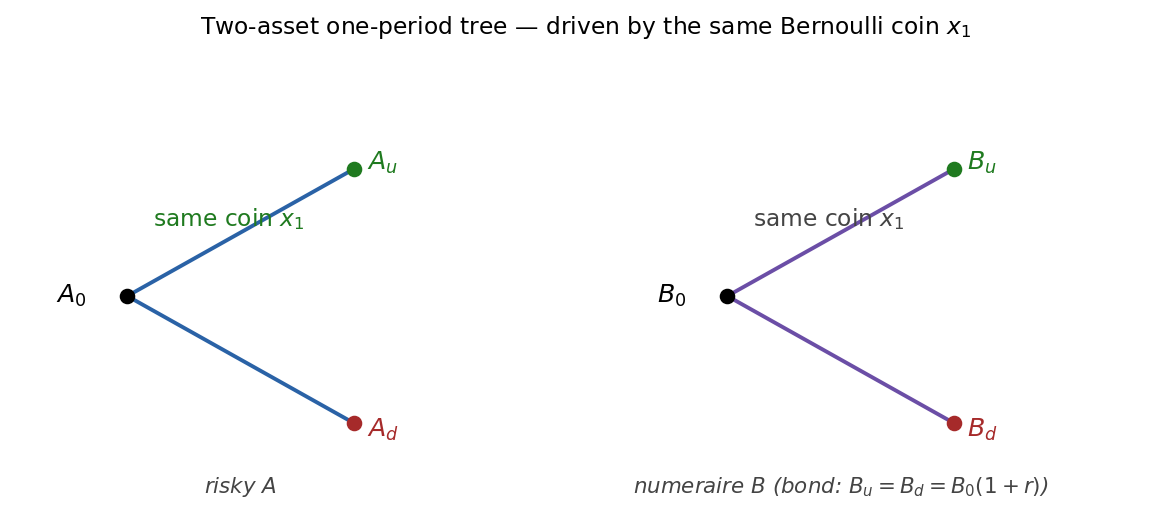
\includegraphics[keepaspectratio]{figures/ch01-two-asset-tree.png}}
\caption{Two-asset one-period tree driven by the same Bernoulli coin}
\end{figure}

\emph{Two parallel one-period trees: risky \(A\) and numeraire \(B\)
branch on the same Bernoulli coin \(x_1\). The bond case sets
\(B_u = B_d = B_0(1+r)\).}

The ``same coin'' assumption is the discrete-time avatar of ``one
Brownian motion'' in continuous time: it matches risk dimension to hedge
dimension and forces market completeness. The general \(B_u \neq B_d\)
setup extends to FX and stochastic-interest-rate models.

\subsection{2.1 Portfolio value}\label{portfolio-value}

Introduce a portfolio \((\alpha,\beta)\) holding \(\alpha\) units of
\(A\) and \(\beta\) units of \(B\):

\[V_0 \;=\; \alpha A_0 + \beta B_0, \tag{2.1}\]

\[V_1 \;=\; \alpha A_1 + \beta B_1. \tag{2.2}\]

Weights are signed: \(\alpha < 0\) is a short position in \(A\),
\(\beta < 0\) is borrowing at the bond rate. Self-financing is automatic
across the single \([0,1]\) interval (no rebalancing event); §7 imposes
it explicitly in the multi-period setting. The map
\((\alpha, \beta) \mapsto (V_1^u, V_1^d)\) is linear with matrix rows
\((A_u, B_u)\) and \((A_d, B_d)\); invertibility
(\(A_u B_d \neq A_d B_u\)) is exactly market completeness, revisited in
§5.

\subsection{2.2 Definition of arbitrage}\label{definition-of-arbitrage}

An arbitrage strategy (portfolio) \((\alpha,\beta)\) is one such that

\[\text{(i)} \quad V_0 = 0, \tag{2.3}\]

\[\text{(ii)} \quad \exists\, t \text{ s.t. } \quad \text{(a)} \;\; \mathbb{P}(V_t \geq 0) = 1 \quad\text{(never lose)}, \tag{2.4}\]

\[\hspace{3.5cm} \text{(b)} \;\; \mathbb{P}(V_t > 0) > 0 \quad\text{(sometimes win)}. \tag{2.5}\]

In plain English: enter at zero cost, never lose, sometimes win --- a
free lunch. The ``weak'' form (2.5) (positive gain on a
positive-probability set) is the version that delivers the EMM in the
FFT.

\subsection{2.3 Sign-sanity toy trees}\label{sign-sanity-toy-trees}

Three toy trees illustrate when the definition fires:

\begin{itemize}
\tightlist
\item
  Tree (a): \(0 \to \{1, 0\}\) --- arbitrage (cost 0 today, outcome
  \(\geq 0\) always, positive sometimes).
\item
  Tree (b): \(0 \to \{1, -1\}\) --- not an arbitrage (down-state loses).
\item
  Tree (c): \(0 \to \{1, 1\}\) --- arbitrage (pays 1 for sure at cost
  0).
\end{itemize}

Sandwich check on \(A_0/B_0\):

{\def\LTcaptype{none} % do not increment counter
\begin{longtable}[]{@{}
  >{\centering\arraybackslash}p{(\linewidth - 10\tabcolsep) * \real{0.1667}}
  >{\centering\arraybackslash}p{(\linewidth - 10\tabcolsep) * \real{0.1667}}
  >{\centering\arraybackslash}p{(\linewidth - 10\tabcolsep) * \real{0.1667}}
  >{\centering\arraybackslash}p{(\linewidth - 10\tabcolsep) * \real{0.1667}}
  >{\centering\arraybackslash}p{(\linewidth - 10\tabcolsep) * \real{0.1667}}
  >{\centering\arraybackslash}p{(\linewidth - 10\tabcolsep) * \real{0.1667}}@{}}
\toprule\noalign{}
\begin{minipage}[b]{\linewidth}\centering
Tree label
\end{minipage} & \begin{minipage}[b]{\linewidth}\centering
\(A_0\)
\end{minipage} & \begin{minipage}[b]{\linewidth}\centering
\(A_d\)
\end{minipage} & \begin{minipage}[b]{\linewidth}\centering
\(A_u\)
\end{minipage} & \begin{minipage}[b]{\linewidth}\centering
Check \(A_d/B_d < A_0/B_0 < A_u/B_u\)? (with \(B\equiv 1\))
\end{minipage} & \begin{minipage}[b]{\linewidth}\centering
Verdict
\end{minipage} \\
\midrule\noalign{}
\endhead
\bottomrule\noalign{}
\endlastfoot
\((-)\) & \(10\) & \(5\) & \(20\) & \(5 < 10 < 20\) & No arb \\
\((+)\) & \(2\) & \(4\) & \(15\) & \(4 \not< 2\) & Arb \\
\((14\ldots)\) & \(\approx 14\) & \(0\) & \(0\) & violates & Arb \\
\end{longtable}
}

For tree \((-)\):
\(q = (A_0 - A_d)/(A_u - A_d) = (10 - 5)/(20 - 5) = 1/3\). If
\(A_0/B_0\) sits strictly between the two relative-price leaves the
model is viable; outside, one leaf dominates.

\subsection{2.4 Scaled-tree arbitrage
illustration}\label{scaled-tree-arbitrage-illustration}

Bond tree \(1 \to \{1+r, 1+r\}\) vs.~asset tree \(1 \to \{1, 1\}\). With
\(\alpha\) in the asset and \(-\alpha\) in the bond, the zero-cost
portfolio pays \(\{(1-r)\alpha,\; -\alpha r\}\). Arbitrage would require

\[\begin{pmatrix} 1-r > 0 \\ -r < 0 \end{pmatrix} \quad \text{or} \quad \begin{pmatrix} 1-r < 0 \\ -r > 0 \end{pmatrix}, \tag{2.6}\]

which simplify to the impossible sign-combinations

\[\boxed{\; r > 0 \text{ and } r < 1 \;} \quad \Vert \quad \boxed{\; r < 0 \text{ and } r > 1 \;} \tag{2.7}\]

so for reasonable \(r\) no arb exists; the practical upshot is the
standard ordering (2.8) below.

\subsection{2.5 The standard ordering}\label{the-standard-ordering}

\[A_0 \in (A_d, A_u), \qquad A_u > A_d, \qquad B_0 > 0. \tag{2.8}\]

The ``up''/``down'' labelling is WLOG; positivity of \(B\) lets us form
ratios \(A/B\). Strict inequalities are the discrete analogue of
\(\sigma > 0\) in Black--Scholes.

\begin{center}\rule{0.5\linewidth}{0.5pt}\end{center}

\section{\texorpdfstring{3. No-Arbitrage Bound on
\(A_0\)}{3. No-Arbitrage Bound on A\_0}}\label{no-arbitrage-bound-on-a_0}

Absence of arbitrage forces \(A_0\) to lie strictly between its
discounted up and down values. We show it twice --- bond case first,
then general numeraire.

\subsection{3.1 Absolute-price derivation (bond
case)}\label{absolute-price-derivation-bond-case}

With \(B_u = B_d = B_0(1+r)\), impose \(V_0 = 0\):

\[\beta \;=\; -\,\alpha\,\frac{A_0}{B_0}. \tag{3.1}\]

A zero-cost portfolio is parameterised by the single number \(\alpha\).
Substitute into the terminal values:

\[\text{up: } \;\; \alpha A_u + \beta B_0(1+r) \;=\; \bigl(A_u - (1+r)A_0\bigr)\alpha, \tag{3.2}\]

\[\text{down: } \;\; \alpha A_d + \beta B_0(1+r) \;=\; \bigl(A_d - (1+r)A_0\bigr)\alpha. \tag{3.3}\]

If both brackets share a sign, an appropriate \(\alpha\) creates a free
lunch. The only viable case is opposite signs, and by \(A_u > A_d\) the
up-bracket is the positive one:

\[A_u - (1+r)A_0 > 0 \quad\text{and}\quad A_d - (1+r)A_0 < 0. \tag{3.4}\]

These combine to

\[\boxed{\; A_d \;<\; A_0(1+r) \;<\; A_u \;} \qquad \text{(no-arb)}. \tag{3.5}\]

I.e. the forward price \(A_0(1+r)\) must lie strictly between the two
future spot values:

\begin{figure}
\centering
\pandocbounded{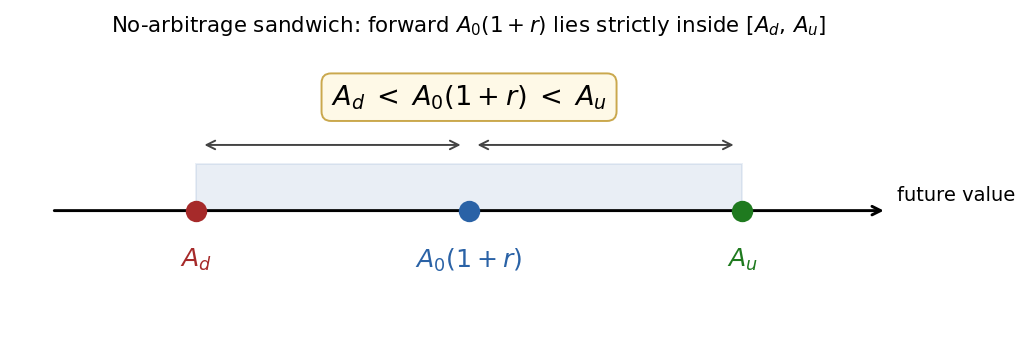
\includegraphics[keepaspectratio]{figures/ch01-no-arb-sandwich.png}}
\caption{No-arbitrage sandwich on the future-value axis}
\end{figure}

\emph{The forward price \(A_0(1+r)\) must sit strictly between the two
future spot leaves \(A_d\) and \(A_u\) --- any other ordering admits an
arbitrage.}

\begin{figure}
\centering
\pandocbounded{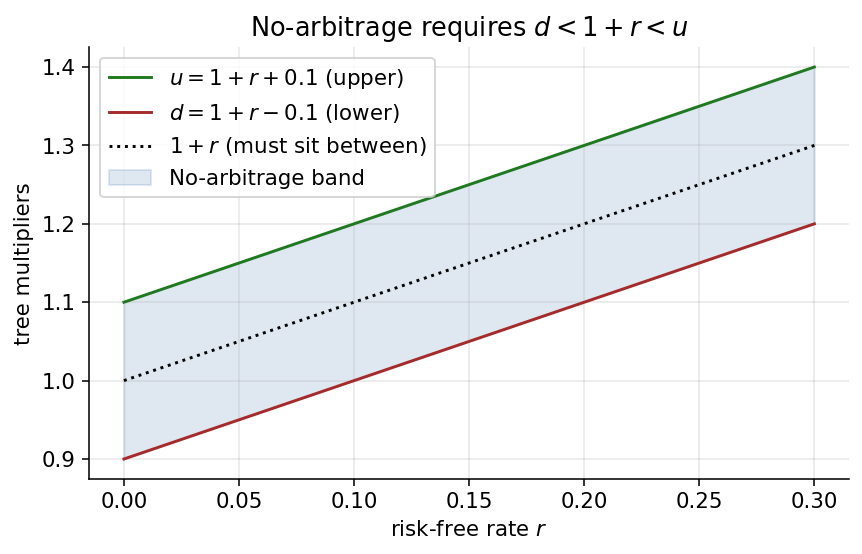
\includegraphics[keepaspectratio]{figures/ch01-arbitrage-region.png}}
\caption{No-arbitrage requires d \textless{} 1+r \textless{} u}
\end{figure}

\emph{No-arbitrage requires} \(d < 1+r < u\).

\(A_0(1+r)\) is the \emph{forward price} of \(A\); the sandwich is the
only configuration with no dominance. In gross-return form, this is the
textbook ``\(d < 1+r < u\)''.

\subsection{3.2 Relative-price derivation (general
numeraire)}\label{relative-price-derivation-general-numeraire}

The bond's role was purely as a clock; any strictly positive numeraire
\(B\) works the same way. With \(\beta = -\alpha A_0/B_0\):

\[\alpha A_u + \beta B_u \;=\; \alpha\!\left(A_u - \frac{A_0}{B_0}\,B_u\right), \tag{3.6}\]

\[\alpha A_d + \beta B_d \;=\; \alpha\!\left(A_d - \frac{A_0}{B_0}\,B_d\right). \tag{3.7}\]

For no arbitrage the two bracketed factors must have opposite signs:

\[\left.\begin{array}{l} A_u - \dfrac{A_0}{B_0}\, B_u \;>\; 0 \\[4pt] A_d - \dfrac{A_0}{B_0}\, B_d \;<\; 0 \end{array}\right\} \quad\text{all other cases lead to arb.} \tag{3.8}\]

(Implicit non-degeneracy: the \(2\times 2\) payoff matrix
\(\bigl(\begin{smallmatrix}A_u & A_d \\ B_u & B_d\end{smallmatrix}\bigr)\)
is non-singular, equivalently \(A_u/B_u \ne A_d/B_d\). This is the
market-completeness hypothesis; for a bond numeraire \(B_u = B_d\) it
holds automatically, for a general numeraire it must be imposed.)

Equivalently, dividing through by \(B_u, B_d > 0\):

\[\boxed{\;\frac{A_d}{B_d} \;<\; \frac{A_0}{B_0} \;<\; \frac{A_u}{B_u}\;} \qquad \text{(no-arbitrage condition)}. \tag{3.9}\]

In the bond case (3.9) reduces to (3.5). The numeraire-free form
generalises to FX (foreign bond), swaptions (annuity), and spread
options (one of the underlyings).

\subsection{\texorpdfstring{3.3 Restatement as existence of a
risk-neutral weight
\(q\)}{3.3 Restatement as existence of a risk-neutral weight q}}\label{restatement-as-existence-of-a-risk-neutral-weight-q}

Convert the inequality into an equality. (3.9) is equivalent to:
\(\exists\, q \in (0,1)\) such that

\[\boxed{\;\frac{A_0}{B_0} \;=\; q\,\frac{A_u}{B_u} \;+\; (1-q)\,\frac{A_d}{B_d}\;} \;\;\Longleftrightarrow\;\; \text{no arbitrage.} \tag{3.10}\]

A number lies strictly between two endpoints iff it is a convex
combination with weights in \((0,1)\). Rearranging:
\(q = (A_0/B_0 - A_d/B_d)/(A_u/B_u - A_d/B_d)\) --- the relative
position of the current relative price within the leaf interval,
depending only on observable prices, not on \(p\) or utility. For an
asset with positive excess return \(q < p\): \(\mathbb{Q}\) tilts weight
to the down-state, the Girsanov shift \(\mu - r\) that §8 makes
explicit.

Equivalently,

\[\tilde A_0 \;=\; \mathbb{E}^{\mathbb{Q}}\!\left[\, \tilde A_1 \,\right], \qquad\text{where}\qquad \tilde A_t \;=\; \frac{A_t}{B_t} \quad\text{(relative price)}, \tag{3.11}\]

under \(\mathbb{Q}\) with up-probability \(q\). The relative price
\(\tilde A\) is a \emph{\(\mathbb{Q}\)-martingale} --- zero expected
drift in numeraire units. The same \(q\) then prices every contingent
claim written on \((A,B)\).

\begin{center}\rule{0.5\linewidth}{0.5pt}\end{center}

\section{4. A Third Asset: Replication and Arbitrage-Free
Pricing}\label{a-third-asset-replication-and-arbitrage-free-pricing}

Add a contingent claim \(C\) with payoff \((C_u, C_d)\). Its price is
pinned down uniquely by \((A,B)\). Two demonstrations: \(q\)-consistency
here, explicit replication in §5.

\begin{figure}
\centering
\pandocbounded{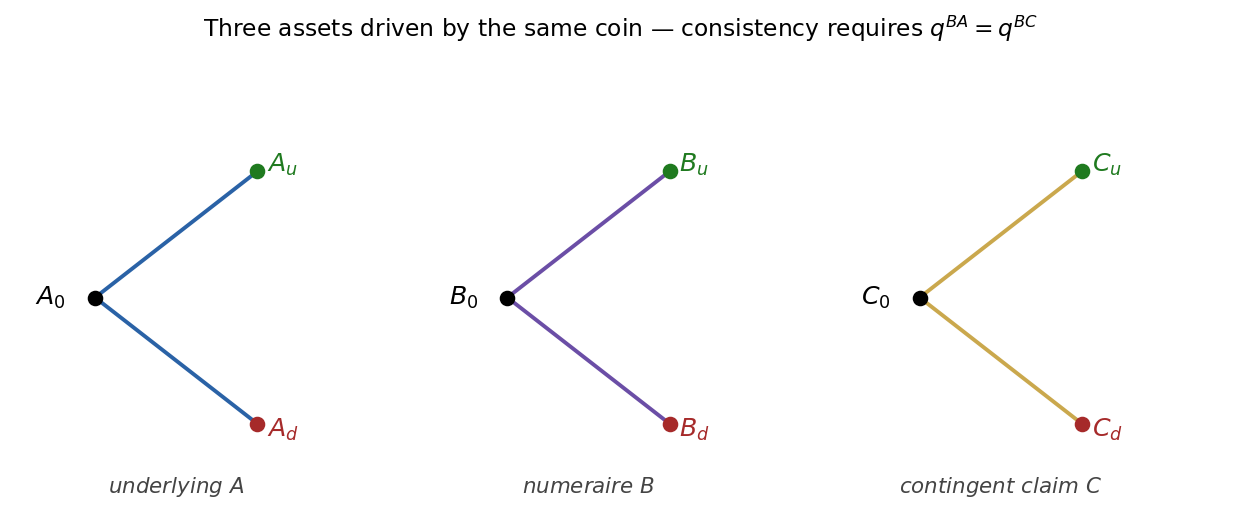
\includegraphics[keepaspectratio]{figures/ch01-three-asset-tree.png}}
\caption{Three assets sharing one Bernoulli coin}
\end{figure}

\emph{Underlying \(A\), numeraire \(B\), and contingent claim \(C\) ---
all three branch on the same coin. A single EMM exists iff the implied
risk-neutral weights \(q^{BA}\) and \(q^{BC}\) agree.}

Each of \(A\) and \(C\), when priced in units of \(B\), must be a
martingale under some \(q \in (0,1)\):

\[\tilde A_0^B \;=\; \mathbb{E}^{\mathbb{Q}}\!\left[\,\tilde A_1^B\,\right] \;\;\longrightarrow\;\; q^{BA} \in (0,1), \tag{4.1}\]

\[\tilde C_0^B \;=\; \mathbb{E}^{\mathbb{Q}}\!\left[\,\tilde C_1^B\,\right] \;\;\longrightarrow\;\; q^{BC} \in (0,1). \tag{4.2}\]

If \(q^{BA} \neq q^{BC}\) no single EMM exists --- the FFT signal of
arbitrage. With \(q^{BA}\) extracted from \((A,B)\), the fair \(C_0\)
must satisfy

\[\frac{C_0}{B_0} \;\stackrel{?}{=}\; \frac{C_u}{B_u}\,q^{BA} \;+\; \frac{C_d}{B_d}\,(1 - q^{BA}). \tag{4.3}\]

Disagreement signals mispricing.

\subsection{4.1 Numerical example --- mispriced third
asset}\label{numerical-example-mispriced-third-asset}

Three trees:

\begin{figure}
\centering
\pandocbounded{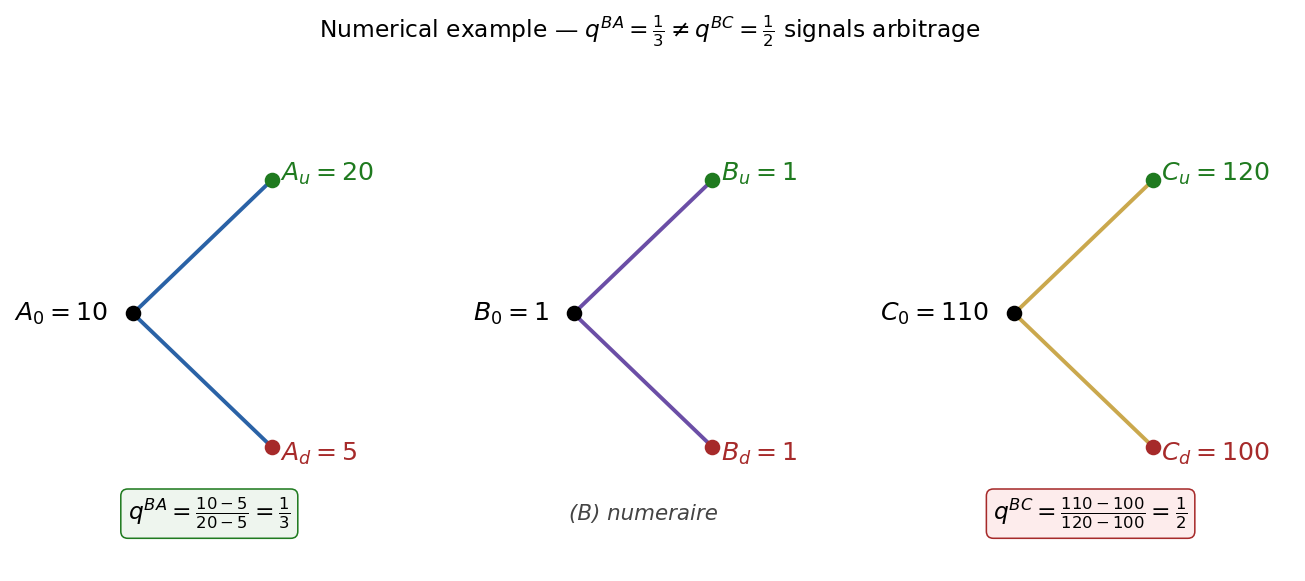
\includegraphics[keepaspectratio]{figures/ch01-three-asset-numerical.png}}
\caption{Numerical three-asset tree with mismatched risk-neutral
weights}
\end{figure}

\emph{Numerical leaves: \(A: 10\to\{20,5\}\), \(B\equiv 1\),
\(C: 110\to\{120,100\}\). The implied weights \(q^{BA}=\tfrac{1}{3}\)
and \(q^{BC}=\tfrac{1}{2}\) disagree --- no single EMM exists, hence
arbitrage.}

Step 1 --- \(q^{BA}\) from \((A,B)\) via (3.10):

\[10 \;=\; 20\, q^{BA} + 5\,(1 - q^{BA}) \;\;\Rightarrow\;\; q^{BA} = \tfrac{1}{3}. \tag{4.4}\]

Step 2 --- extract \(q^{BC}\) from \((C,B)\):

\[110 \;=\; 120\, q^{BC} + 100\,(1 - q^{BC}) \;\;\Rightarrow\;\; q^{BC} = \tfrac{10}{20} = \tfrac{1}{2}. \tag{4.5}\]

Two weights, two answers --- arbitrage.

Step 3 --- forcing \(q = 1/3\) onto \(C\):

\[\widehat C_0 \;=\; 120 \cdot \tfrac{1}{3} \;+\; 100 \cdot \tfrac{2}{3} \;=\; 40 + 66\tfrac{2}{3} \;\approx\; 106.67 \;<\; 110. \tag{4.6}\]

\(C_0 = 110\) is too expensive. Short \(C\) at \(110\), buy the
\((A,B)\) replicant for \(106.67\), pocket \(\$3.33\).

Step 4 --- explicit replication. Match \(C\)'s payoff with
\(V_0 = 110\):

\[V_0 \;=\; 10\alpha + \beta - 110 \;=\; 0 \;\;\Rightarrow\;\; \beta = 110 - 10\alpha. \tag{4.7}\]

Match each leaf (with \(C\) sold short, hence the \(-C_i\) term):

\[\text{up:}\quad 20\alpha + \beta - 120 \;=\; 10\alpha - 10, \tag{4.8}\]

\[\text{down:}\quad 5\alpha + \beta - 100 \;=\; -5\alpha + 10 \;=\; 0. \tag{4.9}\]

The down-leaf gives \(\alpha = 2\), \(\beta = 90\),
\(V_1^{\text{up}} = 10\). Both diagnostics (\(q\)-consistency and
explicit replication) agree.

\begin{center}\rule{0.5\linewidth}{0.5pt}\end{center}

\section{5. Replication --- The General
Recipe}\label{replication-the-general-recipe}

Solve for \((\alpha, \beta)\) reproducing \(C\)'s payoff state-by-state;
the fair price of \(C\) is then the current value of that portfolio.

\[C_u \;=\; \alpha A_u + \beta B_u, \tag{5.1}\]

\[C_d \;=\; \alpha A_d + \beta B_d. \tag{5.2}\]

Then by no-arbitrage

\[C_0 \;=\; \alpha A_0 + \beta B_0, \tag{5.3}\]

otherwise an arbitrage exists (buy cheaper, short expensive). The
\(2\times 2\) system has determinant \(A_u B_d - A_d B_u \neq 0\) iff
\(A_u/B_u \neq A_d/B_d\) --- market completeness.

\subsection{5.1 Closed-form replicating
weights}\label{closed-form-replicating-weights}

Multiply (5.1) by \(B_d\), (5.2) by \(B_u\), subtract:

\[\alpha\,(A_u B_d - A_d B_u) \;=\; C_u B_d - C_d B_u. \tag{5.4}\]

Hence

\[\boxed{\; \alpha \;=\; \frac{C_u B_d - C_d B_u}{A_u B_d - A_d B_u} \;} \tag{5.5}\]

\[\boxed{\; \beta \;=\; \frac{C_u A_d - C_d A_u}{B_u A_d - B_d A_u} \;} \tag{5.6}\]

\(\alpha\) is the \emph{delta} of \(C\). In the bond case it reduces to
\(\alpha = (C_u - C_d)/(A_u - A_d)\), the ``rise over run'' delta;
\(\beta\) is the residual.

\subsection{\texorpdfstring{5.2 Pricing identity and explicit
\(q\)}{5.2 Pricing identity and explicit q}}\label{pricing-identity-and-explicit-q}

Substituting back into (5.3) yields

\[\boxed{\;\frac{C_0}{B_0} \;=\; q\,\frac{C_u}{B_u} \;+\; (1-q)\,\frac{C_d}{B_d}\;} \tag{5.7}\]

where

\[q \;=\; \dfrac{\dfrac{A_0}{B_0} - \dfrac{A_d}{B_d}}{\dfrac{A_u}{B_u} - \dfrac{A_d}{B_d}}. \tag{5.8}\]

The same \(q\) prices every claim. The physical probability \(p\)
appears nowhere: traders disagreeing about \(p\) still agree on \(C_0\)
given observable prices. Self-consistency:

\[\frac{A_0}{B_0} \;=\; q\,\frac{A_u}{B_u} \;+\; (1-q)\,\frac{A_d}{B_d}. \tag{5.9}\]

\subsection{5.3 Bond case: the classical
formula}\label{bond-case-the-classical-formula}

In the bond case \(B_u = B_d = B_0(1+r)\), formulas (5.7)--(5.8) reduce
to

\[C_0 \;=\; \frac{1}{1+r}\bigl(q\,C_u + (1-q)\,C_d\bigr), \qquad q \;=\; \frac{A_0(1+r) - A_d}{A_u - A_d}. \tag{5.10}\]

\(q \in (0,1)\) is precisely the no-arb bound (3.5). Check:
\(A_0 = 100, A_u = 110, A_d = 90, r = 5\%\) gives \(q = 0.75\); a call
struck at 100 prices to \(C_0 \approx 7.14\).

\subsection{5.4 First Fundamental Theorem (one-period
form)}\label{first-fundamental-theorem-one-period-form}

\begin{quote}
No-arbitrage \(\;\Longleftrightarrow\;\)
\(\exists\, \mathbb{Q}\sim\mathbb{P}\) s.t. for all traded assets \(X\),
\(\;\tilde X_0 \;=\; \mathbb{E}^{\mathbb{Q}}[\,\tilde X_1\,]\),
\end{quote}

where

\[\tilde X_t \;=\; \frac{X_t}{B_t} \qquad\text{and}\qquad \mathbb{P}(B_t > 0) = 1 \quad(\text{$B$ is called a numeraire asset}). \tag{5.11}\]

FFT: economic no-free-lunches \(\Leftrightarrow\) probabilistic
existence of an EMM. \(\mathbb{Q} \sim \mathbb{P}\) ensures the two
measures agree on null sets. When \(B_t = e^{rt}\) the associated
\(\mathbb{Q}\) is the \emph{risk-neutral measure}; other numeraires
(stock, forward) appear in later chapters.

In the bond case:

\[\boxed{\; C_0 \;=\; \frac{1}{1+r}\,\mathbb{E}^{\mathbb{Q}}[\,C_1\,] \;} \qquad \text{otherwise } \exists \text{ an arbitrage.} \tag{5.12}\]

(5.12) is the discrete-time prototype of every practical derivatives
pricing formula. In incomplete markets (more risks than instruments)
uniqueness fails --- multiple EMMs, the content of the Second FFT.

\begin{center}\rule{0.5\linewidth}{0.5pt}\end{center}

\section{\texorpdfstring{6. Worked Example --- European Call on \(A\)
Struck at
100}{6. Worked Example --- European Call on A Struck at 100}}\label{worked-example-european-call-on-a-struck-at-100}

Setup: \(A: 100 \to \{120, 90\}\); \(B: 1 \to \{1, 1\}\) (\(r = 0\));
\(C\) payoff \(\{20, 0\}\) (call struck at \(K=100\)).

A call/put gives the right (not obligation) to buy/sell \(A\) at \(K\)
at \(t=1\):

\[\text{Call}(A_1; K) \;=\; \max(A_1 - K,\; 0). \tag{6.1}\]

\[\text{Put}(A_1; K) \;=\; \max(K - A_1,\; 0). \tag{6.2}\]

The payoffs at maturity are the canonical hockey-sticks:

\begin{figure}
\centering
\pandocbounded{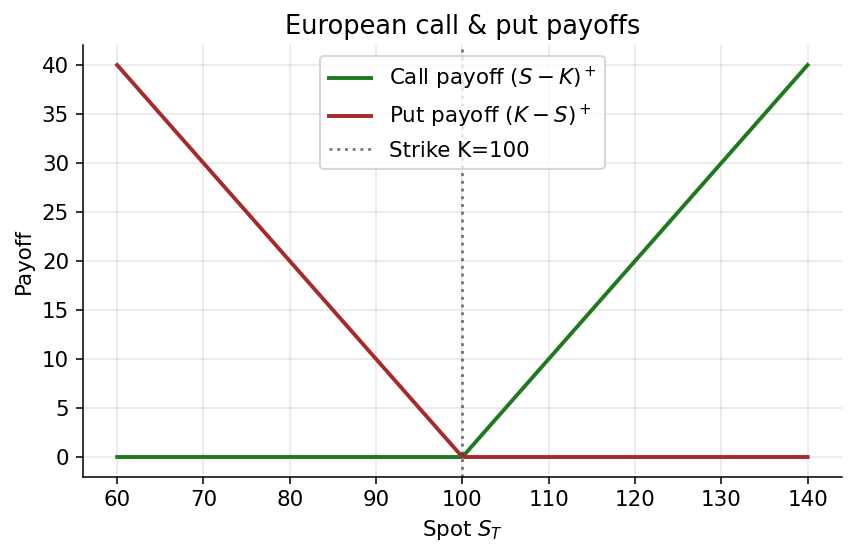
\includegraphics[keepaspectratio]{figures/ch01-payoff.png}}
\caption{European call and put payoffs}
\end{figure}

\emph{Vanilla call and put payoffs.}

\subsection{6.1 Solve replication}\label{solve-replication}

System from (5.1)--(5.2): \(120\alpha + \beta = 20\),
\(90\alpha + \beta = 0\). Subtract: \(\alpha = 2/3\), \(\beta = -60\).

\[\alpha = \tfrac{2}{3}, \qquad \beta = -60. \tag{6.3}\]

Delta \(\alpha = 2/3\) is the discrete analog of \(\Delta = N(d_1)\).

\subsection{\texorpdfstring{6.2 No-arbitrage value of
\(C\)}{6.2 No-arbitrage value of C}}\label{no-arbitrage-value-of-c}

\[C_0 \;=\; \tfrac{2}{3}\cdot 100 + (-60) \;=\; 6\tfrac{2}{3}. \tag{6.4}\]

\subsection{6.3 Cross-check via risk-neutral
formula}\label{cross-check-via-risk-neutral-formula}

From (5.10) with \(r=0\):

\[100 \;=\; q\cdot 120 + (1-q)\cdot 90 \;=\; 90 + 30q \;\;\Rightarrow\;\; q = \tfrac{1}{3}. \tag{6.5}\]

Therefore

\[C_0 \;=\; q \cdot 20 + (1-q)\cdot 0 \;=\; \tfrac{1}{3}\cdot 20 \;=\; 6\tfrac{2}{3}. \tag{6.6}\]

Both methods agree: \(C_0 = 6\tfrac{2}{3}\), independent of \(p\).

\subsection{\texorpdfstring{6.4 Constructing the arbitrage when
\(C_0 = 6\)
(mispriced)}{6.4 Constructing the arbitrage when C\_0 = 6 (mispriced)}}\label{constructing-the-arbitrage-when-c_0-6-mispriced}

Trees:

\begin{figure}
\centering
\pandocbounded{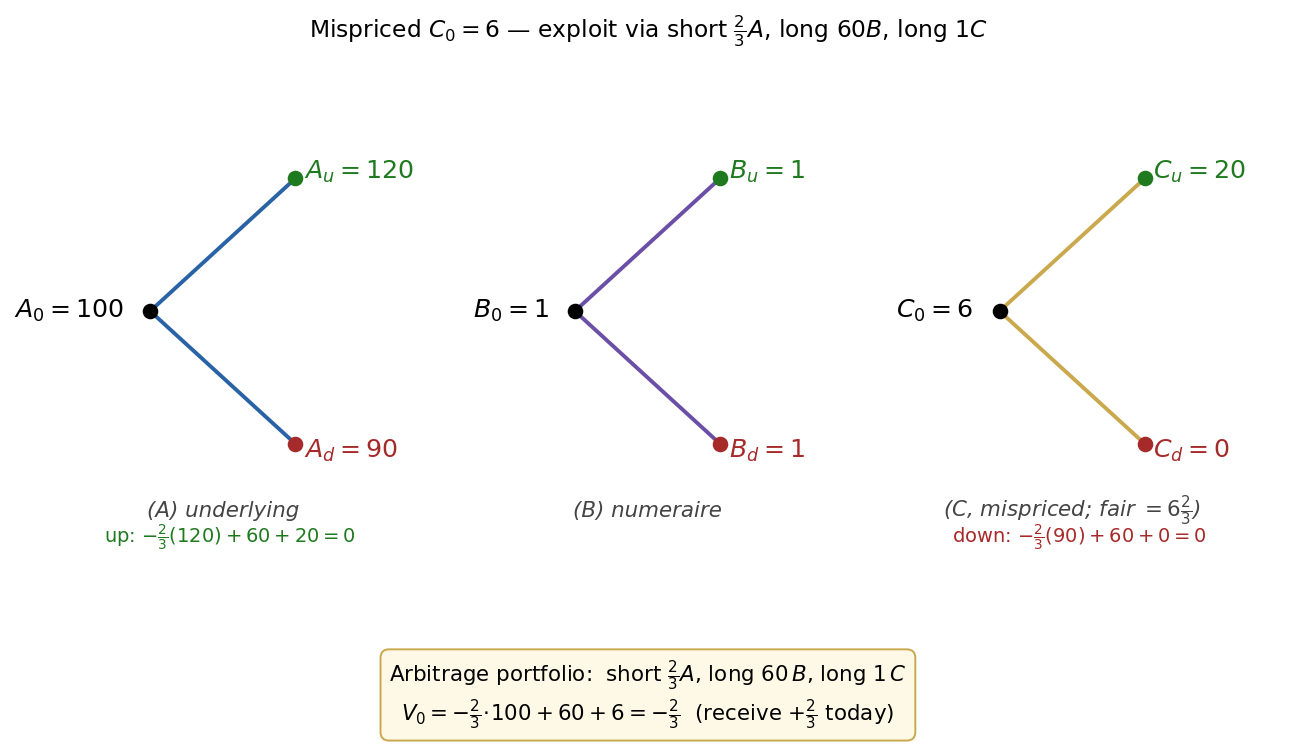
\includegraphics[keepaspectratio]{figures/ch01-mispricing-arb.png}}
\caption{Three-asset tree with explicit arbitrage portfolio}
\end{figure}

\emph{With \(C\) trading at \(6\) (fair value \(6\tfrac{2}{3}\)), the
portfolio short \(\tfrac{2}{3}A\), long \(60B\), long \(1C\) collects
\(+\tfrac{2}{3}\) today and pays exactly \(0\) in both terminal states.}

Strategy: short \(\tfrac{2}{3}\) of \(A\), long \(60\) of \(B\), long
\(1\) unit of \(C\). Initial cashflow:

\[V_0 \;=\; -\tfrac{2}{3}\cdot 100 + 60 + 6 \;=\; -\tfrac{2}{3}. \tag{6.7}\]

i.e.~the arbitrage pays \(+\tfrac{2}{3}\) today. Terminal values:

\[V_1^{(u)} \;=\; -\tfrac{2}{3}\cdot 120 + 60 + 20 \;=\; 0, \tag{6.8}\]

\[V_1^{(d)} \;=\; -\tfrac{2}{3}\cdot 90 + 60 + 0 \;=\; 0. \tag{6.9}\]

The agent pockets \(\tfrac{2}{3}\) today, zero risk at \(t=1\) ---
confirming the no-arb price is \(6\tfrac{2}{3}\).

\begin{center}\rule{0.5\linewidth}{0.5pt}\end{center}

\section{7. Multi-Period Binomial}\label{multi-period-binomial}

Multi-period pricing is one-period pricing applied iteratively backward
through the tree.

Extend to \(N\) periods. Let \(x_n\) be i.i.d. Bernoulli \(\pm 1\) with
\(\mathbb{P}(x_n = +1) = p\). The asset compounds multiplicatively:

\[A_n \;=\; A_{n-1}\, e^{c\, x_n}, \tag{7.1}\]

where \(c\) is a step size (to be calibrated in §8). The tree branches
recursively:

\begin{figure}
\centering
\pandocbounded{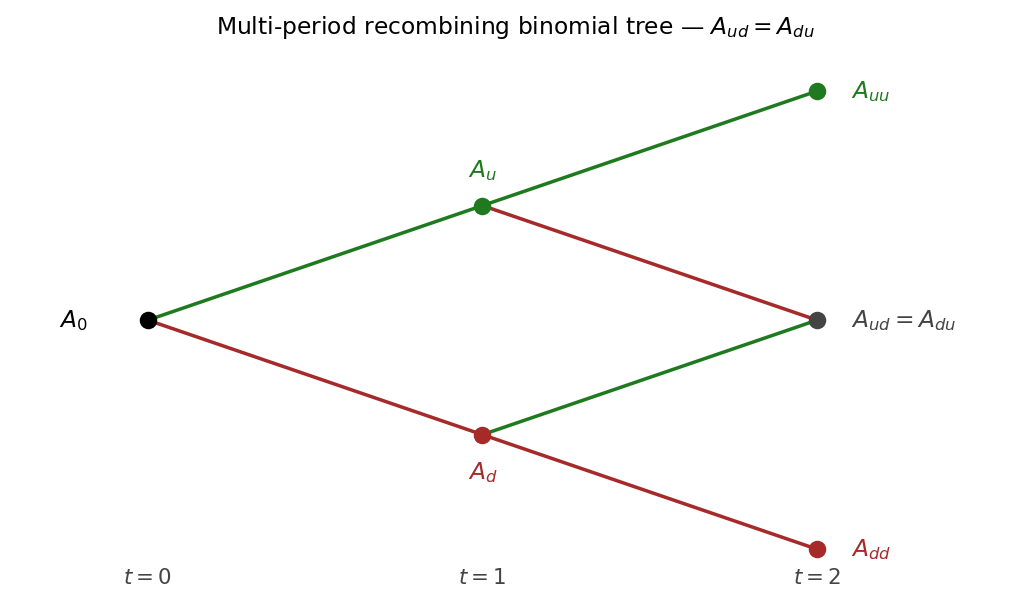
\includegraphics[keepaspectratio]{figures/ch01-multi-period-tree.png}}
\caption{Multi-period recombining binomial tree}
\end{figure}

\emph{Two-step recombining tree:
\(A_0 \to \{A_u, A_d\} \to \{A_{uu}, A_{ud}=A_{du}, A_{dd}\}\). The
middle \(t=2\) node is shared because up-then-down equals down-then-up.}

and likewise for \(B\). These are recombining trees, so
\(A_{ud} = A_{du}\).

The multiplicative update guarantees \(A_n > 0\) on every path and makes
\(\log A_n\) a random walk --- the precondition for the log-normal CLT
limit. After \(N\) steps the terminal price \(A_0 u^k d^{N-k}\) has
\(\mathbb{P}\)-probability \(\binom{N}{k} p^k (1-p)^{N-k}\) --- binomial
in the up-count.

\subsection{7.1 Filtration and
arbitrage}\label{filtration-and-arbitrage}

A strategy \((\alpha_t, \beta_t)\) must be \emph{adapted} to
\(\mathcal{F}_t\) (no peeking at \(A_{t+1}\)). An arbitrage has
\(V_0 = 0\) and \(\exists\, t\) with \(\mathbb{P}(V_t \geq 0) = 1\),
\(\mathbb{P}(V_t > 0) > 0\). We also impose \emph{self-financing}
(\(V_{t+1}^- = V_{t+1}\)) --- without it, every claim would be trivially
replicable by capital injection.

\subsection{7.2 Martingale characterisation
(multi-period)}\label{martingale-characterisation-multi-period}

\[\boxed{\;\text{no arb} \;\Longleftrightarrow\; \exists\, \mathbb{Q} \sim \mathbb{P} \text{ s.t. } \forall\, t < s \text{ and all traded } X, \quad \tilde X_t \;=\; \mathbb{E}^{\mathbb{Q}}\!\left[\, \tilde X_s \,\middle|\, \mathcal{F}_t \,\right]. \;} \tag{7.2}\]

Relative prices are \(\mathbb{Q}\)-martingales. The tower property lets
us price by \emph{backward induction}: roll back one step at a time
using (5.10). For American options, at each node take
\(\max(\text{exercise}, \text{discounted continuation})\).
Path-dependent claims add state variables.

\begin{center}\rule{0.5\linewidth}{0.5pt}\end{center}

\section{8. Matching Drift and
Volatility}\label{matching-drift-and-volatility}

Calibrate \((c, p)\) so the tree approximates geometric Brownian motion
with drift \(\mu\), volatility \(\sigma\):

\[A_n \;=\; A_{n-1}\, e^{\sigma\sqrt{\Delta t}\, x_n} \tag{8.1}\]

(step size \(c = \sigma\sqrt{\Delta t}\)). Matching \(\sigma^2 T\) to
\(N c^2\) forces \(c^2 = \sigma^2 \Delta t\) --- the \emph{diffusive
scaling} that makes the limit Brownian rather than trivial.

\subsection{8.1 Matching the mean of the
log-return}\label{matching-the-mean-of-the-log-return}

Sum \(N\) steps:

\[\ln\!\left(\frac{A_T}{A_0}\right) \;=\; \sigma\sqrt{\Delta t} \;\sum_{n=1}^{N} x_n, \qquad N\,\Delta t = T. \tag{8.2}\]

Take expectation:

\[\mathbb{E}\!\left[\,\ln\!\frac{A_T}{A_0}\,\right] \;=\; \sigma\sqrt{\Delta t}\,\cdot N\,(2p - 1) \;=\; (\mu - \tfrac{1}{2}\sigma^2)\, T. \tag{8.3}\]

The target \((\mu - \tfrac{1}{2}\sigma^2)T\) is the Itô correction for
GBM. Solve for \(p\):

\[2p - 1 \;=\; \frac{\mu - \tfrac{1}{2}\sigma^2}{\sigma}\,\sqrt{\Delta t}, \tag{8.4}\]

\[\boxed{\; p \;=\; \tfrac{1}{2}\!\left[\, 1 \;+\; \frac{\mu - \tfrac{1}{2}\sigma^2}{\sigma}\,\sqrt{\Delta t}\,\right]. \;} \tag{8.5}\]

For \(A\) to grow on average at \(e^{\mu T}\), \(\log A\) must grow at
\((\mu - \tfrac{1}{2}\sigma^2)T\) --- the Itô penalty. Equity with
\(\mu = 10\%\), \(\sigma = 20\%\), \(\Delta t = 1/252\) gives
\(p \approx 0.513\) (a \(1.3\%\) daily tilt that aggregates to \(8\%\)
annual log-drift over \(252\) steps).

\subsection{8.2 Matching the variance}\label{matching-the-variance}

\[\mathbb{V}\!\left[\,\ln\!\frac{A_T}{A_0}\,\right] \;=\; \sigma^2\,\Delta t\,\cdot N\,\mathbb{V}[x_i]. \tag{8.6}\]

For the Bernoulli \(\pm 1\):

\[\mathbb{V}[x_i] \;=\; \mathbb{E}[x_i^2] - (\mathbb{E}[x_i])^2 \;=\; 1 - \left(\frac{\mu - \tfrac{1}{2}\sigma^2}{\sigma}\right)^{\!2}\Delta t. \tag{8.7}\]

Hence

\[\mathbb{V}\!\left[\,\ln\!\frac{A_T}{A_0}\,\right] \;=\; \sigma^2\, T \cdot \left(1 - \left(\frac{\mu - \tfrac{1}{2}\sigma^2}{\sigma}\right)^{\!2}\Delta t\right). \tag{8.8}\]

As \(\Delta t \to 0\) the variance tends to \(\sigma^2 T\).

\subsection{\texorpdfstring{8.3 Risk-neutral probability \(q\) for the
calibrated
tree}{8.3 Risk-neutral probability q for the calibrated tree}}\label{risk-neutral-probability-q-for-the-calibrated-tree}

The calculation parallels §8.1 with \(\mu \mapsto r\). Bank account at
rate \(r\):

\[B_t \;=\; e^{r t}, \qquad B_n \;=\; B_{n-1}\, e^{r\,\Delta t}. \tag{8.9}\]

The martingale identity

\[\frac{A_t}{B_t} \;=\; \mathbb{E}^{\mathbb{Q}}\!\left[\,\frac{A_s}{B_s}\,\middle|\, \mathcal{F}_t\,\right] \tag{8.10}\]

applied to one step gives

\[\frac{A_{n-1}}{B_{n-1}} \;=\; \frac{A_{n-1}}{B_{n-1}}\, e^{\sigma\sqrt{\Delta t} - r\Delta t}\, q \;+\; \frac{A_{n-1}}{B_{n-1}}\, e^{-\sigma\sqrt{\Delta t} - r\Delta t}\,(1-q). \tag{8.11}\]

Cancel \(A_{n-1}/B_{n-1}\) and solve:

\[q \;=\; \frac{e^{r\Delta t} - e^{-\sigma\sqrt{\Delta t}}}{e^{\sigma\sqrt{\Delta t}} - e^{-\sigma\sqrt{\Delta t}}}. \tag{8.12}\]

\emph{CRR form.} Writing \(u = e^{\sigma\sqrt{\Delta t}}\) and
\(d = e^{-\sigma\sqrt{\Delta t}}\), (8.12) becomes the familiar
Cox--Ross--Rubinstein formula

\[q \;=\; \frac{e^{r\Delta t} - d}{u - d}. \tag{8.13}\]

\(d < e^{r\Delta t} < u\) is exactly \(q \in (0,1)\). (8.13) is the
workhorse of discrete-time option pricing.

\subsection{\texorpdfstring{8.4 Small-\(\Delta t\) expansion of
\(q\)}{8.4 Small-\textbackslash Delta t expansion of q}}\label{small-delta-t-expansion-of-q}

Using \(e^x \sim 1 + x + \tfrac{1}{2}x^2 + o(x^2)\):

Numerator:

\[\text{num} \;=\; \big(1 + r\Delta t\big) - \big(1 - \sigma\sqrt{\Delta t} + \tfrac{1}{2}\sigma^2\Delta t\big) + \cdots \;=\; \sigma\sqrt{\Delta t} + \big(r - \tfrac{1}{2}\sigma^2\big)\Delta t + \cdots \tag{8.14}\]

Denominator:

\[\text{denom} \;=\; \big(1 + \sigma\sqrt{\Delta t} + \tfrac{1}{2}\sigma^2\Delta t\big) - \big(1 - \sigma\sqrt{\Delta t} + \tfrac{1}{2}\sigma^2\Delta t\big) + \cdots \;=\; 2\sigma\sqrt{\Delta t} + \cdots \tag{8.15}\]

Ratio:

\[q \;=\; \tfrac{1}{2}\!\left[\,1 \;+\; \frac{r - \tfrac{1}{2}\sigma^2}{\sigma}\,\sqrt{\Delta t}\,\right] + \cdots \tag{8.16}\]

This matches (8.5) with \(\mu \mapsto r\): the swap \(\mu \mapsto r\)
\emph{is} the Girsanov shift from \(\mathbb{P}\) to \(\mathbb{Q}\) in
one line --- the equity risk premium \(\mu - r\) absorbed into the coin
bias.

\[\mathbb{E}^{\mathbb{Q}}\!\left[\,\ln\!\frac{A_T}{A_0}\,\right] \;=\; \big(r - \tfrac{1}{2}\sigma^2\big)\, T, \tag{8.17}\]

\[\mathbb{V}^{\mathbb{Q}}\!\left[\,\ln\!\frac{A_T}{A_0}\,\right] \;=\; \sigma^2\, T + \xi\,\Delta t, \tag{8.18}\]

with \(\xi \Delta t \to 0\). Volatility survives the measure change
(Girsanov shifts drifts only) --- this is why \(\sigma\) is calibrated
from market prices without ever estimating \(\mu\). Inverting
(5.10)/(8.13) at a quoted option price gives the \emph{implied
volatility}.

\begin{center}\rule{0.5\linewidth}{0.5pt}\end{center}

\section{9. Limiting Distribution}\label{limiting-distribution}

As \(N \to \infty\) the calibrated tree converges to a log-normal
distribution --- equivalently, GBM. §11 gives the rigorous CF proof.
Take \(N \to \infty\) in (8.2):

\[\ln\!\left(\frac{A_T}{A_0}\right) \;=\; \sigma\sqrt{\Delta t}\,\sum_{n=1}^{N} x_n \;\xrightarrow[N \to +\infty]{d}\; \mathcal{N}(\,\cdot\,;\,\cdot\,), \tag{9.1}\]

with

\[\text{mean} = \big(\mu - \tfrac{1}{2}\sigma^2\big)\, T, \qquad \text{var} = \sigma^2\, T. \tag{9.2}\]

CLT on \(N\) scaled coin flips with bias (8.5). Equivalently:

\[A_T \;\stackrel{d}{=}\; A_0\, e^{(\mu - \frac{1}{2}\sigma^2)\, T \;+\; \sigma\sqrt{T}\, Z}, \qquad Z \sim_{\mathbb{P}} \mathcal{N}(0;1). \tag{9.3}\]

Taking the expectation (MGF of a Gaussian):

\[\mathbb{E}[A_T] \;=\; A_0\, e^{(\mu - \frac{1}{2}\sigma^2)T} \cdot \mathbb{E}\!\left[\, e^{\sigma\sqrt{T}\, Z}\,\right] \;=\; A_0\, e^{(\mu - \frac{1}{2}\sigma^2)T} \cdot e^{\frac{1}{2}\sigma^2 T} \;=\; A_0\, e^{\mu T}. \tag{9.4}\]

The Itô \(-\tfrac{1}{2}\sigma^2 T\) in the median exponent and the
\(+\tfrac{1}{2}\sigma^2 T\) from the MGF cancel: \(\mu\) is the growth
rate of the \emph{expectation}, \(\mu - \tfrac{1}{2}\sigma^2\) that of
the \emph{log-median}. Under \(\mathbb{Q}\),
\(\mathbb{E}^{\mathbb{Q}}[A_T] = A_0 e^{rT}\).

\begin{center}\rule{0.5\linewidth}{0.5pt}\end{center}

\section{\texorpdfstring{10. Existence of Martingale Measure
\(\Rightarrow\) No
Arbitrage}{10. Existence of Martingale Measure \textbackslash Rightarrow No Arbitrage}}\label{existence-of-martingale-measure-rightarrow-no-arbitrage}

The proof of one direction of the FFT --- short, general, no
completeness required.

Setup. \(A_t^{(1)}, \ldots, A_t^{(n)} \geq 0\) \(\mathbb{P}\)-a.s.,
\(B_t > 0\) \(\mathbb{P}\)-a.s., \(t \in \{0, 1\}\).

Hypothesis. Suppose \(\exists\, \mathbb{Q} \sim \mathbb{P}\) s.t.

\[\frac{A_0^{(k)}}{B_0} \;=\; \mathbb{E}^{\mathbb{Q}}\!\left[\,\frac{A_1^{(k)}}{B_1}\,\right], \qquad k = 1,\ldots, n. \tag{10.1}\]

Claim. Any portfolio \((\alpha^{(1)},\ldots,\alpha^{(n)},\beta)\) such
that

\[\mathbb{P}(V_1 \geq 0) = 1, \qquad \mathbb{P}(V_1 > 0) > 0, \tag{10.2}\]

must have \(V_0 > 0\), ruling out arbitrage (which would require
\(V_0 = 0\)).

Derivation. Compute \(V_0\) directly:

\[V_0 \;=\; \beta\, B_0 + \sum_{k=1}^{n} \alpha^{(k)} A_0^{(k)}. \tag{10.3}\]

Factor out \(B_0\) and use the martingale hypothesis:

\[V_0 \;=\; B_0\!\left[\,\beta \;+\; \sum_{k=1}^{n} \alpha^{(k)}\,\frac{A_0^{(k)}}{B_0}\,\right] \;=\; B_0\,\mathbb{E}^{\mathbb{Q}}\!\left[\,\frac{B_1}{B_1}\,\beta \;+\; \sum_{k=1}^{n} \alpha^{(k)}\,\frac{A_1^{(k)}}{B_1}\,\right]. \tag{10.4}\]

Combining:

\[V_0 \;=\; B_0\,\mathbb{E}^{\mathbb{Q}}\!\left[\,\frac{\beta\, B_1 \;+\; \sum_{k=1}^{n} \alpha^{(k)} A_1^{(k)}}{B_1}\,\right] \;=\; B_0\,\mathbb{E}^{\mathbb{Q}}\!\left[\,\frac{V_1}{B_1}\,\right] \;>\; 0. \tag{10.5}\]

The last inequality uses \(B_0, B_1 > 0\) and (since
\(\mathbb{Q}\sim\mathbb{P}\)) \(V_1 \geq 0\) \(\mathbb{Q}\)-a.s. with
\(V_1 > 0\) on a \(\mathbb{Q}\)-positive set. Hence \(V_0 > 0\) and no
portfolio satisfying (10.2) can have \(V_0 = 0\). \(\blacksquare\)

The converse (no arb \(\Rightarrow \exists\mathbb{Q}\)) requires a
separating-hyperplane argument on the zero-cost payoff cone
(Dalang--Morton--Willinger).

\begin{center}\rule{0.5\linewidth}{0.5pt}\end{center}

\section{11. Central Limit Theorem for the Binomial
Tree}\label{central-limit-theorem-for-the-binomial-tree}

CF proof that the calibrated tree of §8 converges to the Gaussian
claimed in §9.

Setup. Let

\[X \;=\; \sigma\sqrt{\Delta t}\,\sum_{n=1}^{N} x_i, \qquad \Delta t \;=\; \frac{T}{N}. \tag{11.1}\]

With the calibrated probabilities

\[\mathbb{P}(x_i = +1) \;=\; p \;=\; \tfrac{1}{2}\!\left[\,1 \;+\; \frac{\mu - \tfrac{1}{2}\sigma^2}{\sigma}\,\sqrt{\Delta t}\,\right], \tag{11.2}\]

\[\mathbb{P}(x_i = -1) \;=\; 1 - p \;=\; \tfrac{1}{2}\!\left[\,1 \;-\; \frac{\mu - \tfrac{1}{2}\sigma^2}{\sigma}\,\sqrt{\Delta t}\,\right]. \tag{11.3}\]

Let \(\hat\mu \;\doteq\; \mu - \tfrac{1}{2}\sigma^2\) (log-drift).

Goal. Show that as \(N \to +\infty\),

\[X \;\xrightarrow[N\to+\infty]{d}\; \mathcal{N}\!\big(\hat\mu\, T,\; \sigma^2 T\big). \tag{11.4}\]

Method. Characteristic function. Compute

\[\mathbb{E}\!\left[\,e^{i u X}\,\right] \;=\; \mathbb{E}\!\left[\,e^{i u \sigma\sqrt{\Delta t}\,\sum_{n=1}^{N} x_i}\,\right] \;=\; \left(\,\mathbb{E}\!\left[\,e^{i u \sigma\sqrt{\Delta t}\, x_i}\,\right]\,\right)^{N}. \tag{11.5}\]

CFs factor over independent sums and uniquely determine distributions
(Lévy continuity). Expand the inner expectation:

\[\mathbb{E}\!\left[\,e^{i u \sigma\sqrt{\Delta t}\, x_i}\,\right] \;=\; \mathbb{E}\!\left[\,1 + i u \sigma\sqrt{\Delta t}\, x_i - \tfrac{1}{2}u^2\sigma^2\,\Delta t\, x_i^2 + o(\Delta t)\,\right] \tag{11.6}\]

\[= 1 + i u \sigma\sqrt{\Delta t}\,\mathbb{E}[x_i] - \tfrac{1}{2}u^2\sigma^2\,\Delta t\,\mathbb{E}[x_i^2] + o(\Delta t). \tag{11.7}\]

Next compute:

\[\mathbb{E}[x_i] \;=\; 2p - 1 \;=\; \frac{\hat\mu}{\sigma}\,\sqrt{\Delta t}, \tag{11.8}\]

and

\[\mathbb{E}[x_i^2] \;=\; 1. \tag{11.9}\]

Substituting:

\[\boxed{\;\mathbb{E}\!\left[\,e^{i u \sigma\sqrt{\Delta t}\, x_i}\,\right] \;=\; 1 + i u\, \hat\mu\, \Delta t \;-\; \tfrac{1}{2} u^2 \sigma^2\, \Delta t \;+\; o(\Delta t).\;} \tag{11.10}\]

The \(\sqrt{\Delta t}\) cancels because
\(\mathbb{E}[x_i] = O(\sqrt{\Delta t})\) --- exactly the calibration
(8.5).

So:

\[\mathbb{E}\!\left[\,e^{i u X}\,\right] \;=\; \left(1 + \big(i u\,\hat\mu - \tfrac{1}{2}\sigma^2 u^2\big)\,\Delta t \;+\; o(\Delta t)\right)^{N} \xrightarrow[N\to\infty]{}\; e^{\,\big(i u\,\hat\mu - \tfrac{1}{2}\sigma^2 u^2\big)\, T}, \tag{11.11}\]

using the classical limit

\[\left(1 + \tfrac{a}{N}\right)^{N} \;\xrightarrow[N\to\infty]{}\; e^{a}. \tag{11.12}\]

Recognising the right-hand side of (11.11) as the characteristic
function of a Gaussian with mean \(\hat\mu T\) and variance
\(\sigma^2 T\):

\[\boxed{\;X \;\xrightarrow[N\to\infty]{d}\; \mathcal{N}\!\big(\hat\mu\, T;\; \sigma^2 T\big). \;} \tag{11.13}\]

CF of \(\mathcal{N}(m, v)\) is \(e^{i u m - \tfrac{1}{2} v u^2}\);
matching to (11.11) gives \(m = \hat\mu T\), \(v = \sigma^2 T\), exactly
(9.2). \(A_T\) is log-normal in the limit --- geometric Brownian motion
derived from scratch without stochastic calculus.

\begin{center}\rule{0.5\linewidth}{0.5pt}\end{center}

\section{Worked Examples}\label{worked-examples}

\subsection{\texorpdfstring{WE-1. Why \(\mathbb{P}\)-expectation is not
a
price}{WE-1. Why \textbackslash mathbb\{P\}-expectation is not a price}}\label{we-1.-why-mathbbp-expectation-is-not-a-price}

Take a tree with \(A_0 = 100\), \(A_u = 110\), \(A_d = 95\), \(r = 0\),
and physical probability \(p = 0.6\). The naïve discounted expectation
is \(0.6 \cdot 110 + 0.4 \cdot 95 = 104\), suggesting the asset is
\emph{under-priced}. But under the risk-neutral measure
\(q = (100 - 95)/(110 - 95) = 1/3\), the discounted expectation is
\(\tfrac13 \cdot 110 + \tfrac23 \cdot 95 = 100\) --- exactly the spot.
Two traders disagreeing about \(p\) would compute different
\(\mathbb{P}\)-expectations; neither is a price. The price is what it
costs to \emph{replicate} the payoff, and replication knows nothing
about \(p\).

\subsection{\texorpdfstring{WE-2. Sign check with three small trees
\textbar{} Tree \textbar{} \(A_0\) \textbar{} \(A_d\) \textbar{} \(A_u\)
\textbar{} Check \(A_d < A_0 < A_u\)? \textbar{} Verdict
\textbar{}}{WE-2. Sign check with three small trees \textbar{} Tree \textbar{} A\_0 \textbar{} A\_d \textbar{} A\_u \textbar{} Check A\_d \textless{} A\_0 \textless{} A\_u? \textbar{} Verdict \textbar{}}}\label{we-2.-sign-check-with-three-small-trees-tree-a_0-a_d-a_u-check-a_d-a_0-a_u-verdict}

\textbar:---:\textbar:---:\textbar:---:\textbar:---:\textbar:---:\textbar:---:\textbar{}
\textbar{} \((-)\) \textbar{} \(10\) \textbar{} \(5\) \textbar{} \(20\)
\textbar{} \(5 < 10 < 20\) \textbar{} No arb \textbar{} \textbar{}
\((+)\) \textbar{} \(2\) \textbar{} \(4\) \textbar{} \(15\) \textbar{}
\(4 \not< 2\) \textbar{} Arb \textbar{} \textbar{} \((14\ldots)\)
\textbar{} \(\approx 14\) \textbar{} \(0\) \textbar{} \(0\) \textbar{}
violates \textbar{} Arb \textbar{}

For tree \((-)\): \(q = (10-5)/(20-5) = 1/3\). Diagnosis is a strict
inequality test, no probabilities required.

\subsection{\texorpdfstring{WE-3. Third asset mispriced - \(A\):
\(10 \to \{20, 5\}\); \(B\): \(1 \to \{1,1\}\) (so \(r=0\)); \(C\):
\(110 \to \{120, 100\}\).}{WE-3. Third asset mispriced - A: 10 \textbackslash to \textbackslash\{20, 5\textbackslash\}; B: 1 \textbackslash to \textbackslash\{1,1\textbackslash\} (so r=0); C: 110 \textbackslash to \textbackslash\{120, 100\textbackslash\}.}}\label{we-3.-third-asset-mispriced---a-10-to-20-5-b-1-to-11-so-r0-c-110-to-120-100.}

\begin{itemize}
\tightlist
\item
  \(q\) from \(A\)-tree: \(q^{BA} = 1/3\). Fair
  \(\widehat C_0 = 120 \cdot \tfrac{1}{3} + 100 \cdot \tfrac{2}{3} \approx 106.67 < 110\).
\item
  Replicating portfolio: \(\alpha = 2\), \(\beta = 90\). Selling \(C\)
  at \(110\) and buying \((2,90)\) in \((A,B)\) gives \(V_0 = 0\),
  \(V_1^{\text{up}} = +10\), \(V_1^{\text{down}} = 0\) --- an arbitrage.
\item
  Internal solve of \(q^{BC}\):
  \(110 = 120 q + 100(1-q) \Rightarrow q^{BC} = 1/2\), inconsistent with
  \(q^{BA} = 1/3\).
\end{itemize}

\subsection{\texorpdfstring{WE-4. European call on \(A\) at strike
\(K=100\) With tree \(100 \to \{120, 90\}\), \(r = 0\),
\(K = 100\):}{WE-4. European call on A at strike K=100 With tree 100 \textbackslash to \textbackslash\{120, 90\textbackslash\}, r = 0, K = 100:}}\label{we-4.-european-call-on-a-at-strike-k100-with-tree-100-to-120-90-r-0-k-100}

{\def\LTcaptype{none} % do not increment counter
\begin{longtable}[]{@{}
  >{\raggedright\arraybackslash}p{(\linewidth - 2\tabcolsep) * \real{0.5000}}
  >{\raggedright\arraybackslash}p{(\linewidth - 2\tabcolsep) * \real{0.5000}}@{}}
\toprule\noalign{}
\begin{minipage}[b]{\linewidth}\raggedright
quantity
\end{minipage} & \begin{minipage}[b]{\linewidth}\raggedright
value
\end{minipage} \\
\midrule\noalign{}
\endhead
\bottomrule\noalign{}
\endlastfoot
\(\alpha\) (shares of \(A\)) & \(2/3\) \\
\(\beta\) (bonds) & \(-60\) \\
\(q\) (risk-neutral prob.) & \(1/3\) \\
no-arb call price \(C_0\) & \(6\tfrac{2}{3}\) \\
arbitrage profit if \(C_0 = 6\) & \(+\tfrac{2}{3}\) at \(t=0\), \(0\) at
\(t=1\) \\
\end{longtable}
}

Put-call parity check: put has payoff \(\{0, 10\}\),
\(P_0 = 2/3 \cdot 10 = 20/3\), so \(C_0 - P_0 = 0 = A_0 - K e^{-rT}\).

\begin{center}\rule{0.5\linewidth}{0.5pt}\end{center}

\section{Key Takeaways}\label{key-takeaways}

\begin{itemize}
\tightlist
\item
  Naive expected-value pricing fails for risk-averse agents: a
  \(\pm 100\) coin-flip is nothing like a \(\pm 10^6\) coin-flip, yet
  they have equal expectation.
\item
  One-period no-arbitrage: \(V_0 = 0\), \(\mathbb{P}(V_t \geq 0) = 1\),
  \(\mathbb{P}(V_t > 0) > 0\) defines an arb; no-arb is equivalent to
  \(A_d/B_d < A_0/B_0 < A_u/B_u\), i.e.~in the bond case
  \(A_d < A_0(1+r) < A_u\).
\item
  Risk-neutral measure: \(\exists\, q \in (0,1)\) such that
  \(A_0/B_0 = q\,A_u/B_u + (1-q)\,A_d/B_d\), with explicit
  \(q = (A_0/B_0 - A_d/B_d)/(A_u/B_u - A_d/B_d)\).
\item
  Replication = pricing: any claim \(C\) with payoffs \((C_u, C_d)\) can
  be synthesised by \((\alpha, \beta)\) in \((A, B)\); formulas
  (5.5)--(5.6). The unique arbitrage-free price is
  \(C_0/B_0 = q\, C_u/B_u + (1-q)\, C_d/B_d\), which in the bond case
  reduces to \(C_0 = \frac{1}{1+r}\mathbb{E}^{\mathbb{Q}}[C_1]\).
\item
  Relative prices are \(\mathbb{Q}\)-martingales --- First Fundamental
  Theorem: no arb \(\Leftrightarrow \exists\, \mathbb{Q}\sim\mathbb{P}\)
  s.t. \(\tilde X_0 = \mathbb{E}^{\mathbb{Q}}[\tilde X_1]\) for every
  traded \(X\).
\item
  Multi-period extension: \(\mathcal{F}_t\)-adapted strategies,
  \(\tilde X_t = \mathbb{E}^{\mathbb{Q}}[\tilde X_s | \mathcal{F}_t]\)
  for all \(t < s\).
\item
  Calibrated tree: \(c = \sigma\sqrt{\Delta t}\) and
  \(p = \tfrac{1}{2}[1 + (\mu - \tfrac{1}{2}\sigma^2)\sqrt{\Delta t}/\sigma]\)
  match log-normal drift \(\mu - \tfrac{1}{2}\sigma^2\) and variance
  \(\sigma^2\) per unit time.
\item
  Risk-neutral \(q\) in continuous calibration:
  \(q = (e^{r\Delta t} - e^{-\sigma\sqrt{\Delta t}})/(e^{\sigma\sqrt{\Delta t}} - e^{-\sigma\sqrt{\Delta t}})\),
  expanding to
  \(\tfrac{1}{2}[1 + (r - \tfrac{1}{2}\sigma^2)\sqrt{\Delta t}/\sigma]\).
  The swap \(\mu \mapsto r\) is the Girsanov shift.
\item
  Limit law:
  \(\ln(A_T/A_0) \xrightarrow{d} \mathcal{N}((\mu - \tfrac{1}{2}\sigma^2)T, \sigma^2 T)\)
  and \(\mathbb{E}[A_T] = A_0 e^{\mu T}\).
\item
  One direction of the FFT proved explicitly: existence of
  \(\mathbb{Q}\) forces
  \(V_0 = B_0\, \mathbb{E}^{\mathbb{Q}}[V_1/B_1] > 0\) for any
  non-negative, non-trivial terminal wealth --- ruling out arbitrage.
\item
  CLT via characteristic functions: \((1 + a/N)^N \to e^a\) produces
  \(\mathbb{E}[e^{iuX}] \to e^{iu\hat\mu T - \frac{1}{2}\sigma^2 u^2 T}\)
  and hence \(X \xrightarrow{d} \mathcal{N}(\hat\mu T, \sigma^2 T)\).
\end{itemize}

\begin{center}\rule{0.5\linewidth}{0.5pt}\end{center}

\section{Reference Formulas}\label{reference-formulas}

Binomial fair-price relation (physical, not a pricing rule):
\[A_0 = \frac{p A_u + (1-p) A_d}{1+r}\]

Arbitrage (definition):
\[V_0 = 0, \qquad \mathbb{P}(V_t \geq 0) = 1, \qquad \mathbb{P}(V_t > 0) > 0\]

No-arbitrage bound (bond case): \[A_d < A_0(1+r) < A_u\]

No-arbitrage bound (general numeraire):
\[\frac{A_d}{B_d} < \frac{A_0}{B_0} < \frac{A_u}{B_u}\]

Risk-neutral probability (general):
\[q = \dfrac{A_0/B_0 - A_d/B_d}{A_u/B_u - A_d/B_d}\]

Risk-neutral probability (bond case):
\[q = \frac{A_0(1+r) - A_d}{A_u - A_d}\]

Replicating portfolio for claim \(C\):
\[\alpha = \frac{C_u B_d - C_d B_u}{A_u B_d - A_d B_u}, \qquad \beta = \frac{C_u A_d - C_d A_u}{B_u A_d - B_d A_u}\]

Risk-neutral pricing (general):
\[\frac{C_0}{B_0} = q\,\frac{C_u}{B_u} + (1-q)\,\frac{C_d}{B_d}\]

Risk-neutral pricing (bond case):
\[C_0 = \frac{1}{1+r}\,\mathbb{E}^{\mathbb{Q}}[C_1] = \frac{1}{1+r}\bigl(q\,C_u + (1-q)\,C_d\bigr)\]

First Fundamental Theorem (one-period):
\[\text{no arb} \;\Longleftrightarrow\; \exists\, \mathbb{Q}\sim\mathbb{P} \text{ s.t. } \tilde X_0 = \mathbb{E}^{\mathbb{Q}}[\tilde X_1]\ \forall\text{ traded } X,\qquad \tilde X_t = X_t/B_t\]

Multi-period martingale characterisation:
\[\text{no arb} \;\Longleftrightarrow\; \exists\, \mathbb{Q}\sim\mathbb{P}:\ \tilde X_t = \mathbb{E}^{\mathbb{Q}}[\tilde X_s | \mathcal{F}_t],\ \forall t<s,\ \forall X\text{ traded}\]

Multiplicative binomial update:
\[A_n = A_{n-1}\, e^{\sigma\sqrt{\Delta t}\, x_n}, \qquad x_n \in \{\pm 1\}\]

Calibrated physical \(p\):
\[p = \tfrac{1}{2}\bigl[1 + \tfrac{\mu - \tfrac{1}{2}\sigma^2}{\sigma}\sqrt{\Delta t}\bigr]\]

Calibrated risk-neutral \(q\) (CRR form):
\[q = \frac{e^{r\Delta t} - d}{u - d}, \qquad u = e^{\sigma\sqrt{\Delta t}},\ d = e^{-\sigma\sqrt{\Delta t}}\]

Small-\(\Delta t\) expansion of \(q\):
\[q \approx \tfrac{1}{2}\bigl[1 + \tfrac{r - \tfrac{1}{2}\sigma^2}{\sigma}\sqrt{\Delta t}\bigr]\]

Log-normal limit distribution:
\[\ln(A_T/A_0) \;\xrightarrow{d}\; \mathcal{N}\bigl((\mu - \tfrac{1}{2}\sigma^2)T,\ \sigma^2 T\bigr), \qquad \mathbb{E}[A_T] = A_0 e^{\mu T}\]

Call and put payoffs:
\[\text{Call}(A_1; K) = \max(A_1 - K,\; 0), \qquad \text{Put}(A_1; K) = \max(K - A_1,\; 0)\]

\newpage

\chapter{Chapter 2 --- Multi-Period Binomial, CRR, and the
FTAP}\label{chapter-2-multi-period-binomial-crr-and-the-ftap}

Chapter 1 established risk-neutral pricing for a single-period two-state
economy. Here we build the explicit multi-period binomial machinery ---
backward induction along a recombining tree --- and its limit the
Cox--Ross--Rubinstein (CRR) model. We present two equivalent CRR
parameterisations: the classical \(A_n = A_{n-1} e^{c\, x_n}\) Bernoulli
lattice, and the ``direct-Gaussian increment'' lattice with the Itô
convexity built into the nodes. We state the Fundamental Theorem of
Asset Pricing (FTAP) and confront non-uniqueness of \(\mathbb{Q}\) when
the tree has more than two states. The chapter closes with the
dynamic-programming recursion for American options.

Themes: - \emph{Completeness vs incompleteness.} Binomial trees are
exactly one-step complete. Add a third branch (default, jump, stoch-vol
state) and uniqueness fails; pricing becomes a \emph{range} and a
risk-preference device selects one representative. - \emph{Backward
induction.} Bellman's dynamic-programming principle handles Americans
and any path-dependence captured by finitely many state variables. Monte
Carlo is the forward-simulation complement, developed in Chapter 9. -
\emph{Numéraire freedom.} The FTAP is silent on which asset deflates;
the choice will be exploited heavily in Chapter 5 (Girsanov) and beyond.

\begin{center}\rule{0.5\linewidth}{0.5pt}\end{center}

\section{2.1 One-Period Review: the No-Arbitrage
Inequality}\label{one-period-review-the-no-arbitrage-inequality}

Start at \(A\) with successors \(A_u > A_d\) and a cash account growing
at \(1+r\). The one-period no-arbitrage inequality is

\[A_d \;<\; A(1 + r) \;<\; A_u \;\iff\; \text{no arb}. \tag{2.1}\]

If \(A(1+r) \leq A_d\) then borrowing cash and buying stock yields
riskless profit; symmetrically for \(A(1+r) \geq A_u\). The forward
price must sit strictly between the two post-states.

Equivalently, any claim \(C\) with terminal values \(C_u, C_d\) admits a
unique arbitrage-free price via \(\mathbb{Q}\):

\[\exists\, \mathbb{Q} \text{ s.t. } C \;=\; \frac{1}{1+r}\,\mathbb{E}^{\mathbb{Q}}[\,C_1\,] \;\iff\; \text{no arb}, \qquad q = \tfrac{A(1+r)-A_d}{A_u-A_d}. \tag{2.2}\]

Together (2.1)--(2.2) form the one-period FTAP, a microcosm of the
general FTAP in §2.5. The weights \(q,1-q\) are \emph{not} physical
probabilities --- they are the unique convex combination making the
discounted asset a one-step martingale. The Radon--Nikodym derivative
\(d\mathbb{Q}/d\mathbb{P}\) is the market's discount of optimism and is
the engine of Girsanov's theorem (Chapter 5).

Worked check. \(A=100, r=5\%, A_u=120, A_d=90\): forward
\(= 105 \in (90,120)\), so \(q = (105-90)/30 = 1/2\). ATM call
(\(K=100\)): \(C = (1/1.05)(0.5\cdot 20) \approx 9.52\). Replicating:
\(\alpha = 2/3, \beta \approx -57.14\), giving
\(2/3\cdot 100 - 57.14 \approx 9.52\) ✓.

\subsection{Case study: Petrobras ADR vs ordinary arbitrage (PBR /
PETR4)}\label{case-study-petrobras-adr-vs-ordinary-arbitrage-pbr-petr4}

The Brazilian oil major Petrobras has two near-identical equity claims
trading in different venues: PETR4 (preferred ordinary shares, traded on
Brazil's B3 exchange in BRL) and PBR (American Depositary Receipts,
traded on NYSE in USD, each ADR representing one ordinary share). By
construction, the no-arbitrage relationship is
\(\text{PBR}_t = \text{PETR4}_t / \text{FX}_t^{\text{BRL/USD}}\), modulo
a small ADR depositary fee. Yet over essentially every trading day from
2018 to 2024, the implied FX rate from \((PETR4, PBR)\) has
\emph{deviated} from the actual BRL/USD spot --- sometimes by 50 to 200
basis points, occasionally more during Brazilian political stress. The
pair is tracked daily by Latin-American equity desks at every major bank
precisely because the deviations represent a concrete, observable
violation of the law of one price.

Read through the FTAP, the trade is the cleanest possible example of why
(2.1)--(2.2) matter. We have three ``assets'': PETR4, PBR, and the
BRL/USD currency forward. Two of them span the same claim --- a unit of
Petrobras equity at time \(T\) --- so the relative price between them
must equal the FX forward, by the same argument that gives (2.1).
Mispricings open because the three venues have different trading hours
(B3 closes at 17:00 BRT, NYSE closes at 16:00 EST), different settlement
cycles (T+2 in Brazil, T+1 in the US post-2024), and different liquidity
profiles. Closing the gap requires simultaneous trades in BRL/USD FX,
PETR4 on B3, and PBR on NYSE --- operationally demanding,
capital-intensive, and exposed to overnight gap risk. The risk-neutral
measure \(\mathbb{Q}\) implied by PETR4 vs the one implied by PBR is
slightly different --- exactly the non-uniqueness of \(\mathbb{Q}\)
flagged at the end of Chapter 1, now in real-world form.

The practitioner lesson is twofold. First, real markets \emph{do}
contain detectable FTAP violations --- they are not theoretical
curiosities. They survive because of trading frictions (FX swap costs,
ADR creation/cancellation fees, time-zone overlap risk) that gate the
pure-arbitrage trade. Second, the price an arbitrageur can actually
realise is the model price \emph{minus} those frictions. When
practitioners say ``the spread is too narrow to trade,'' they mean the
FTAP gap is real but smaller than the friction cost of closing it. The
frictionless model is the \emph{attractor}; the observed deviations
measure the round-trip cost of trading.

\begin{center}\rule{0.5\linewidth}{0.5pt}\end{center}

\section{2.2 Multi-Period Binomial Tree --- Backward
Induction}\label{multi-period-binomial-tree-backward-induction}

Extend the one-step construction to \(N\) steps. Recombination
(\(A_{ud} = A_{du}\)) reduces \(2^N\) terminal nodes to \(N+1\), giving
\(O(N^2)\) pricing complexity. At \(N=250\) daily steps, that's
\(\approx 31{,}000\) node evaluations versus \(2^{250} \approx 10^{75}\)
without recombination. Multiplicative models recombine because
multiplication commutes.

\begin{figure}
\centering
\pandocbounded{
\includegraphics[keepaspectratio]{figures/ch02-recombining-tree.png}}
\caption{Non-recombining \(2^N\) tree vs the recombining \((N+1)\)-node
lattice --- the algorithmic collapse that makes a 250-step daily SPX
lattice feasible on a laptop rather than on the entire memory of the
observable universe}
\end{figure}

At every interior node the claim value is
\(\tfrac{1}{1+r}\mathbb{E}^{\mathbb{Q}}[\text{next-step payoff}]\) with
node-local \(q\). In simple CRR, \(q\) depends only on \((u, d, 1+r)\)
and is global; in state-dependent models (local vol, stochastic rates)
each node has its own \(q\). The backward-induction algorithm is
identical either way.

\subsection{\texorpdfstring{2.2.1 Worked example --- call struck at 100,
maturity
\(T = 2\)}{2.2.1 Worked example --- call struck at 100, maturity T = 2}}\label{worked-example-call-struck-at-100-maturity-t-2}

A two-period non-constant-factor lattice:

\begin{figure}[H]
\centering
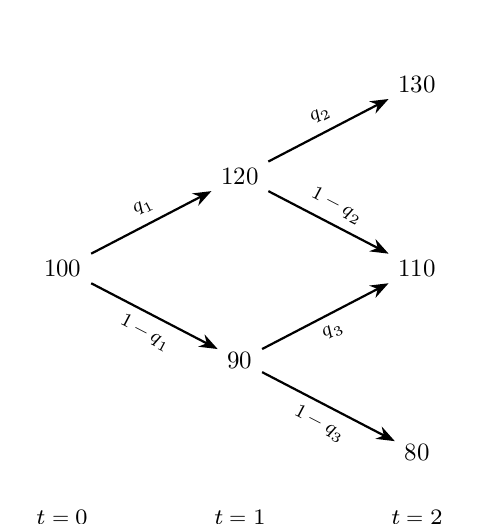
\begin{tikzpicture}[>=Stealth,scale=0.9,every node/.style={font=\small}]
  \node (S00) at (0,0) {$100$};
  \node (S1u) at (2.5,1.3) {$120$};
  \node (S1d) at (2.5,-1.3) {$90$};
  \node (S2uu) at (5,2.6) {$130$};
  \node (S2ud) at (5,0) {$110$};
  \node (S2dd) at (5,-2.6) {$80$};
  \draw[->,thick] (S00) -- node[above,sloped,font=\scriptsize] {$q_1$} (S1u);
  \draw[->,thick] (S00) -- node[below,sloped,font=\scriptsize] {$1-q_1$} (S1d);
  \draw[->,thick] (S1u) -- node[above,sloped,font=\scriptsize] {$q_2$} (S2uu);
  \draw[->,thick] (S1u) -- node[above,sloped,font=\scriptsize] {$1-q_2$} (S2ud);
  \draw[->,thick] (S1d) -- node[below,sloped,font=\scriptsize] {$q_3$} (S2ud);
  \draw[->,thick] (S1d) -- node[below,sloped,font=\scriptsize] {$1-q_3$} (S2dd);
  \node[below=0.6cm,font=\footnotesize\itshape] at (0,-2.6) {$t = 0$};
  \node[below=0.6cm,font=\footnotesize\itshape] at (2.5,-2.6) {$t = 1$};
  \node[below=0.6cm,font=\footnotesize\itshape] at (5,-2.6) {$t = 2$};
\end{tikzpicture}

\textit{Local risk-neutral weights $q_1, q_2, q_3$ — one per branching node — are pinned down by the one-period FTAP applied at each node.}
\end{figure}

with edge-local interest rates \(r_1, r_2, r_3\) on the three
time-\(0 \to 1 \to 2\) edges. The local risk-neutral probabilities
\(q_1, q_2, q_3\) are pinned down by matching the parent to the
discounted expectation of its children:

\[120 \;=\; \frac{1}{1 + r_?}\!\left(\,130\,q_2 \;+\; 110\,(1 - q_2)\,\right) \;\Longrightarrow\; q_2 = \# \tag{2.3}\]

\[90 \;=\; \frac{1}{1 + r_?}\!\left(\,110\,q_3 \;+\; 80\,(1 - q_3)\,\right) \;\Longrightarrow\; q_3 = \# \tag{2.4}\]

\[100 \;=\; \frac{1}{1 + r_?}\!\left(\,120\,q_1 \;+\; 90\,(1 - q_1)\,\right) \;\Longrightarrow\; q_1 = \# \tag{2.5}\]

Payoff @ \(T = 2\). Call struck at \(K = 100\): \(\max(A_T - K, 0)\).
Terminal column \(A_T \in \{130, 110, 110, 80\}\), payoffs
\(\{30, 10, 10, 0\}\). The middle value 110 occurs twice ---
recombination at work; \(\mathbb{Q}\)-probability of reaching it is
\(2q(1-q)\).

Backward step 1 (t = 1 nodes). At the upper intermediate node (stock =
120):

\[C_{1u} \;=\; \frac{1}{1 + r_2}\!\left(\,30\,q_2 \;+\; 10\,(1 - q_2)\,\right) \;=\; \#, \tag{2.7}\]

and at the lower intermediate node (stock = 90, children 110 and 80,
payoffs 10 and 0):

\[C_{1d} \;=\; \frac{1}{1 + r_3}\!\left(\,10\,q_3 \;+\; 0\,(1 - q_3)\,\right) \;=\; \#. \tag{2.8}\]

Backward step 2 (t = 0).

\[C_0 \;=\; \frac{1}{1 + r_1}\!\left(\,C_{1u}\,q_1 \;+\; C_{1d}\,(1 - q_1)\,\right) \;=\; \#. \tag{2.9}\]

\emph{Intuition.} Backward induction is the lattice manifestation of the
tower property
\(\mathbb{E}[\mathbb{E}[X|\mathcal{F}_s]|\mathcal{F}_t] = \mathbb{E}[X|\mathcal{F}_t]\)
for \(t \le s\). Computing step by step (vs the one-shot
\(C_0 = \mathbb{E}^{\mathbb{Q}}[e^{-rT}C_T]\)) lets the same sweep
handle path-dependent payoffs (Asians, lookbacks), barriers, and
American exercise (§2.8), with \(O(N^2)\) complexity in the state
variables.

\begin{figure}
\centering
\pandocbounded{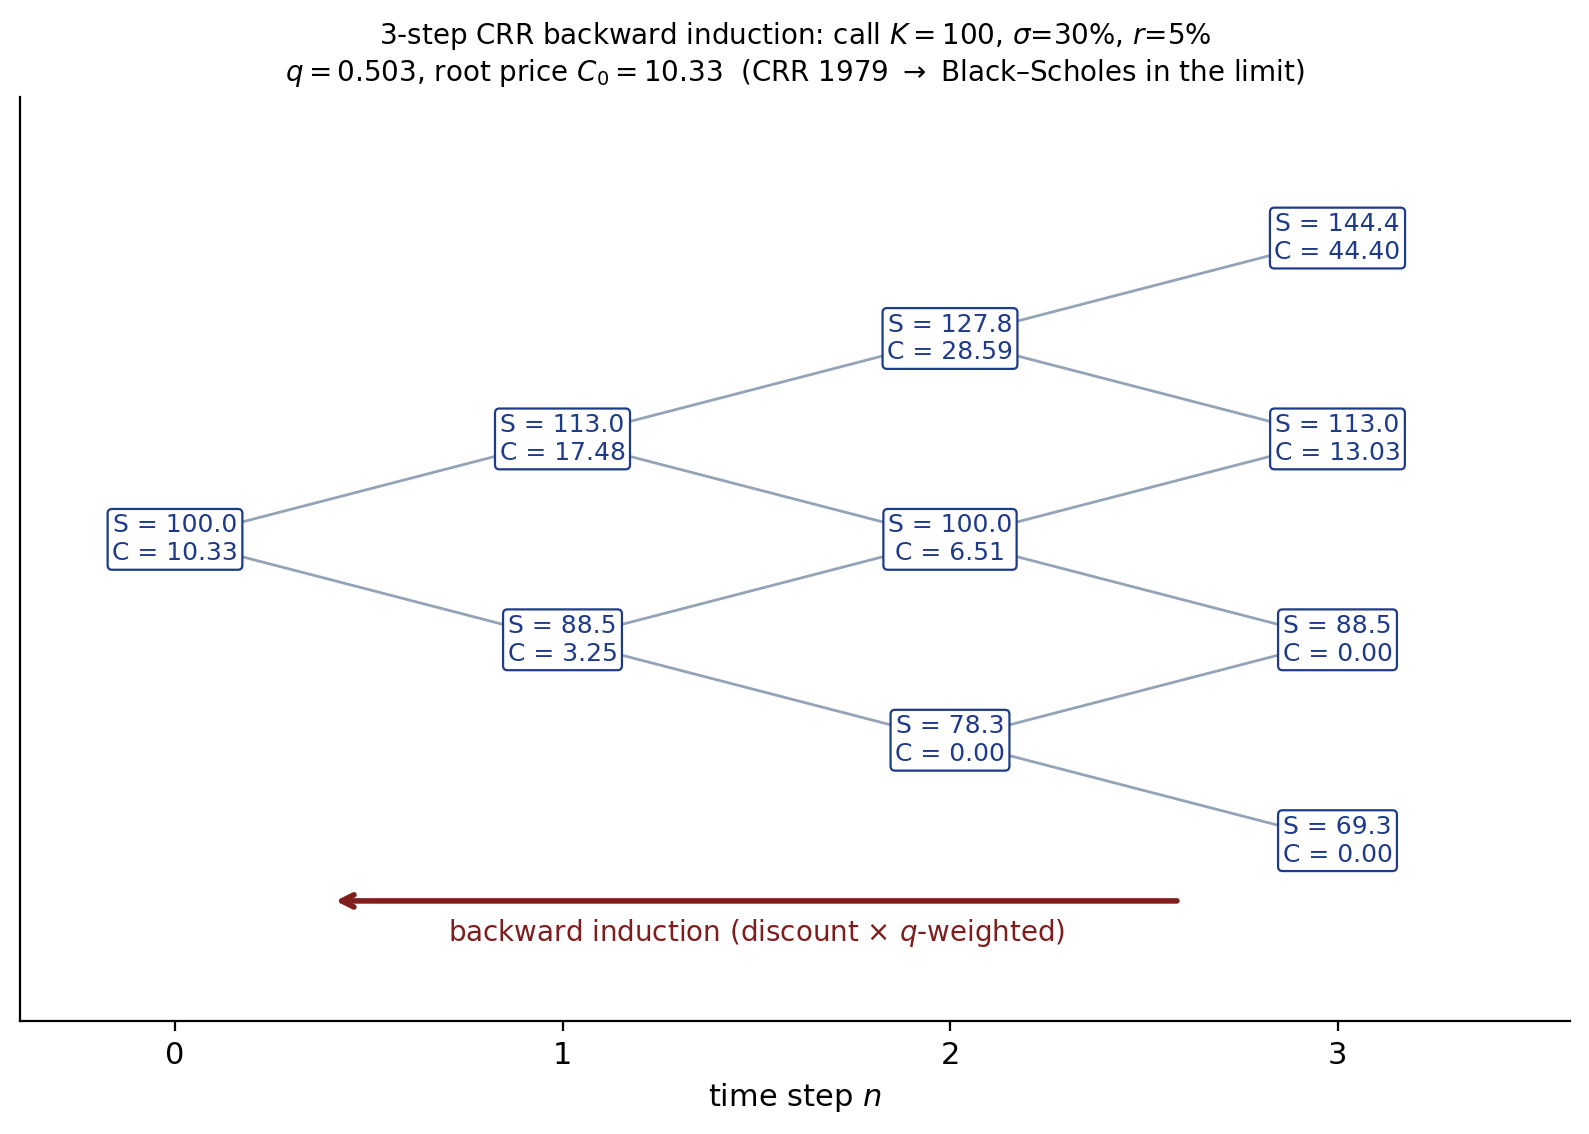
\includegraphics[keepaspectratio]{figures/ch02-backward-induction.png}}
\caption{Backward induction on a 3-step CRR tree pricing an ATM call:
terminal payoffs roll back through the \(q\)-weighted discount at each
node to the root value \(C_0\) --- the algorithm Cox-Ross-Rubinstein
proved converges to Black-Scholes in 1979 and every option-pricing
library still ships today}
\end{figure}

\subsection{2.2.2 Path-weights and the CRR telescoping
identity}\label{path-weights-and-the-crr-telescoping-identity}

If \(r_1 = r_2 = r_3 = r\) the root price collapses to

\[C_0 \;=\; \frac{1}{(1 + r)^N}\,\mathbb{E}^{\mathbb{Q}}\!\left[\,C_T\,\right] \;=\; (1+r)^{-N}\sum_{k=0}^{N}\binom{N}{k} q^k(1-q)^{N-k}(A_0 u^k d^{N-k}-K)_+. \tag{2.10}\]

As \(N\to\infty\) with
\(u = e^{\sigma\sqrt{\Delta t}}, d = e^{-\sigma\sqrt{\Delta t}}\), the
binomial distribution converges to normal (de Moivre--Laplace) and the
sum to the Black--Scholes integral. Convergence is \(O(1/N)\) with
oscillation; Richardson extrapolation accelerates. The distribution of
up-moves is Binomial\((N, q)\), giving closed-form moments:
\(\mathbb{E}^{\mathbb{Q}}[A_T] = A_0(1+r)^N\) (martingale) and
\(\mathbb{V}^{\mathbb{Q}}[\ln A_T] \to \sigma^2 T\).

\begin{center}\rule{0.5\linewidth}{0.5pt}\end{center}

\section{2.3 The Cox--Ross--Rubinstein (CRR) Model --- Bernoulli
Parameterisation}\label{the-coxrossrubinstein-crr-model-bernoulli-parameterisation}

CRR (1979) showed the binomial lattice converges to Black--Scholes as
\(\Delta t \to 0\) and gives a tractable pricing tool for Americans and
exotics. In step \(\Delta t\), replace \(1+r\) with \(e^{r\Delta t}\)
(cleaner algebra; aligns with \(B_T = e^{rT}\) in the limit). Up-moves
multiply by \(e^c\), down-moves by \(e^{-c}\) (symmetric \(\pm c\) for
recombination).

\[A_n \;=\; A_{n-1}\, e^{c\, x_n}, \qquad x_n \stackrel{iid}{\sim} \text{Bernoulli}(\pm 1), \;\; \mathbb{P}(x = +1) = p. \tag{2.12}\]

Symmetric Bernoulli \(\pm 1\) is the simplest random variable with two
states per step (one-step completeness), symmetric placement
(recombination), and iid increments. The choice cleanly separates move
size (\(c\)) from directional bias (\(p - \tfrac12\)).

Iterating \(N = T/\Delta t\) steps,

\[A_T \;=\; A_0\,e^{c\,X_N}, \qquad X_N := \sum_{n=1}^{N} x_n. \tag{2.13}\]

\subsection{2.3.1 Moments of the increment
sum}\label{moments-of-the-increment-sum}

Calibrate by moment-matching: two free parameters \((p, c)\) match two
empirical moments \((\mu, \sigma^2)\). Linearity plus iid Bernoulli:

\[\mathbb{E}[X_N] \;=\; \sum_{n=1}^{N}\mathbb{E}[x_n] \;=\; N\bigl(\,+1\cdot p + (-1)(1-p)\,\bigr) \;=\; N\,(2p - 1) \;=\; \mu\,\Delta t\, N, \tag{2.14}\]

\[\mathbb{V}[X_N] \;=\; N\,\mathbb{V}[x_1] \;=\; N\!\left(\,\mathbb{E}[x_1^2] - (\mathbb{E}[x_1])^2\,\right) \;=\; N\bigl(1 - (2p - 1)^2\bigr) \;=\; \sigma^2\,\Delta t\, N. \tag{2.15}\]

The data feed in \(\mu\) and \(\sigma^2\) as annualised log-return mean
and variance from a price series via

\[\ln(S_2 / S_1) \;=\; r_1, \quad \ln(S_3 / S_2) \;=\; r_2, \quad \dots \tag{2.16}\]

\[\widehat{\mu\,\Delta t} \;=\; \frac{1}{M}\sum_{m=1}^{M} r_m \quad\text{(annualised return)}, \tag{2.17}\]

\[\widehat{\sigma^2\,\Delta t} \;=\; \frac{1}{M}\sum_{m=1}^{M} (r_m - \widehat{\mu\Delta t})^2 \quad\text{(annualised variance)}. \tag{2.18}\]

\subsection{\texorpdfstring{2.3.2 Solving for the CRR parameters
\((p, c)\)}{2.3.2 Solving for the CRR parameters (p, c)}}\label{solving-for-the-crr-parameters-p-c}

Solving (2.14)--(2.15) simultaneously, using \(\mathbb{E}[x^2] = c^2\):

\[\mathbb{V}[X_N^{c\text{-scaled}}] \;=\; c^2 N\bigl(1 - (2p - 1)^2\bigr) \;=\; \sigma^2 \Delta t\, N, \tag{2.19}\]

one obtains the Cox--Ross--Rubinstein up-step and physical probability:

\[\boxed{\; c \;=\; \sigma\sqrt{\Delta t} + \cdots, \qquad p \;=\; \tfrac{1}{2}\!\left(\,1 \;+\; \frac{\mu}{\sigma}\,\sqrt{\Delta t}\,\right) + \cdots. \;} \tag{2.20}\]

\emph{Intuition.} Variance match gives \(c = \sigma\sqrt{\Delta t}\);
mean match gives a small \(O(\sqrt{\Delta t})\) bias in \(p\). Worked:
\(\sigma = 20\%, \mu = 10\%, \Delta t = 1/252\) gives
\(c \approx 0.0126\) (per-step \(\pm 1.27\%\) moves) and
\(p \approx 0.516\). The \(\sqrt{\Delta t}\) scaling of \(c\) is the
universal scaling of Brownian motion --- at daily horizon, diffusion
(\(\sigma\sqrt{\Delta t}\)) is \(\sim\!16\times\) larger than drift
(\(\mu\Delta t\)), which is why short-horizon returns look like noise.

\subsection{\texorpdfstring{2.3.3 Converting to the
\(\mathbb{Q}\)-probability}{2.3.3 Converting to the \textbackslash mathbb\{Q\}-probability}}\label{converting-to-the-mathbbq-probability}

The \(\mathbb{P}\to\mathbb{Q}\) transformation re-weights probabilities
so the expected return matches the riskless rate \(r\). Risk-neutral
pricing on the \(e^{\pm c}\) tree:

\[A \;=\; e^{-r\Delta t}\, \mathbb{E}^{\mathbb{Q}}[\,A_{n}\,] \;=\; e^{-r\Delta t}\!\left(\,q\, A\, e^{\sigma\sqrt{\Delta t}} \;+\; (1 - q)\, A\, e^{-\sigma\sqrt{\Delta t}}\,\right), \tag{2.21}\]

giving

\[\boxed{\; q \;=\; \frac{e^{r\Delta t} - e^{-\sigma\sqrt{\Delta t}}}{e^{+\sigma\sqrt{\Delta t}} - e^{-\sigma\sqrt{\Delta t}}}. \;} \tag{2.22}\]

Small-\(\Delta t\) expansion. Using
\(e^{\pm z} \sim 1 \pm z + \tfrac{1}{2}z^2 + \cdots\) in both numerator
and denominator,

\[q \;\sim\; \tfrac{1}{2}\!\left(\,1 \;+\; \frac{r - \tfrac{1}{2}\sigma^2}{\sigma}\,\sqrt{\Delta t}\,\right) + \cdots \tag{2.23}\]

\[p \;\sim\; \tfrac{1}{2}\!\left(\,1 \;+\; \frac{\mu}{\sigma}\,\sqrt{\Delta t}\,\right) + \cdots \qquad\text{(for comparison, under } \mathbb{P}\text{).} \tag{2.24}\]

The boxed formula (2.22) is \emph{exact} at finite \(\Delta t\); (2.23)
is leading-order. The \(\mathbb{P} \to \mathbb{Q}\) shift replaces the
log-return drift \(\mu\) by \(r - \tfrac12\sigma^2\) --- the Itô
convexity adjustment shows up already at the lattice level, before any
stochastic calculus. The deeper reason is the geometric-vs-arithmetic
mean gap: \(\mathbb{E}[e^X] \ge e^{\mathbb{E}[X]}\). A naïve simulator
that uses just \(r\) (no \(-\tfrac12\sigma^2\)) over-prices calls by
\(\sim e^{\sigma^2 T/2}\) --- a 28\% bias at \(\sigma=50\%, T=2\).

\subsection{\texorpdfstring{2.3.4 Log-moments under \(\mathbb{P}\) vs
\(\mathbb{Q}\)}{2.3.4 Log-moments under \textbackslash mathbb\{P\} vs \textbackslash mathbb\{Q\}}}\label{log-moments-under-mathbbp-vs-mathbbq}

Combining (2.13) with (2.20) / (2.23),

\[\mathbb{E}^{\mathbb{P}}\!\left[\ln(A_T / A_0)\right] \;=\; \mu\, T, \qquad \mathbb{V}^{\mathbb{P}}\!\left[\ln(A_T / A_0)\right] \;=\; \sigma^2\, T, \tag{2.25}\]

\[\mathbb{E}^{\mathbb{Q}}\!\left[\ln(A_T / A_0)\right] \;=\; \bigl(r - \tfrac{1}{2}\sigma^2\bigr)\, T, \qquad \mathbb{V}^{\mathbb{Q}}\!\left[\ln(A_T / A_0)\right] \;=\; \sigma^2\, T. \tag{2.26}\]

\begin{quote}
Slogan. ``\(\mathbb{P}\) and \(\mathbb{Q}\) variances are identical''
--- ``\(\mathbb{P}\) and \(\mathbb{Q}\) means are \emph{not}''.
\end{quote}

\emph{Intuition.} Girsanov at one line: a change of equivalent measure
tilts drifts but \emph{cannot} change volatility --- quadratic variation
is measure-invariant because it is a pathwise quantity, not a
probabilistic one. Implied volatility (\(\mathbb{Q}\)-world) and
realised volatility (\(\mathbb{P}\)-world) measure the same \(\sigma^2\)
in principle; their empirical gap is the \emph{variance risk premium},
traded actively via VIX futures vs realised S\&P 500 variance.

\subsection{2.3.5 Continuous-time limit --- lognormal
asset}\label{continuous-time-limit-lognormal-asset}

Apply the CLT to \(X_N = \sum x_n\) as \(N \to \infty\) with
\(N\Delta t = T\) fixed:

\[\ln(A_T / A_0) \;=\; X_N \;\xrightarrow[N\to\infty]{d,\ \mathbb{P}}\; \mathcal{N}\!\left(\,\mu T,\; \sigma^2 T\,\right), \tag{2.27}\]

\[\ln(A_T / A_0) \;=\; X_N \;\xrightarrow[N\to\infty]{d,\ \mathbb{Q}}\; \mathcal{N}\!\left(\,(r - \tfrac{1}{2}\sigma^2)T,\; \sigma^2 T\,\right). \tag{2.28}\]

Equivalently, in distribution,

\[A_T \;\stackrel{d}{=}\; A_0\, e^{\mu T \;+\; \sigma\sqrt{T}\, Z_{\mathbb{P}}}, \qquad Z_{\mathbb{P}} \sim \mathcal{N}(0, 1), \tag{2.29}\]

\[A_T \;\stackrel{d}{=}\; A_0\, e^{(r - \tfrac{1}{2}\sigma^2)T \;+\; \sigma\sqrt{T}\, Z_{\mathbb{Q}}}, \qquad Z_{\mathbb{Q}} \sim \mathcal{N}(0, 1). \tag{2.30}\]

\begin{figure}
\centering
\pandocbounded{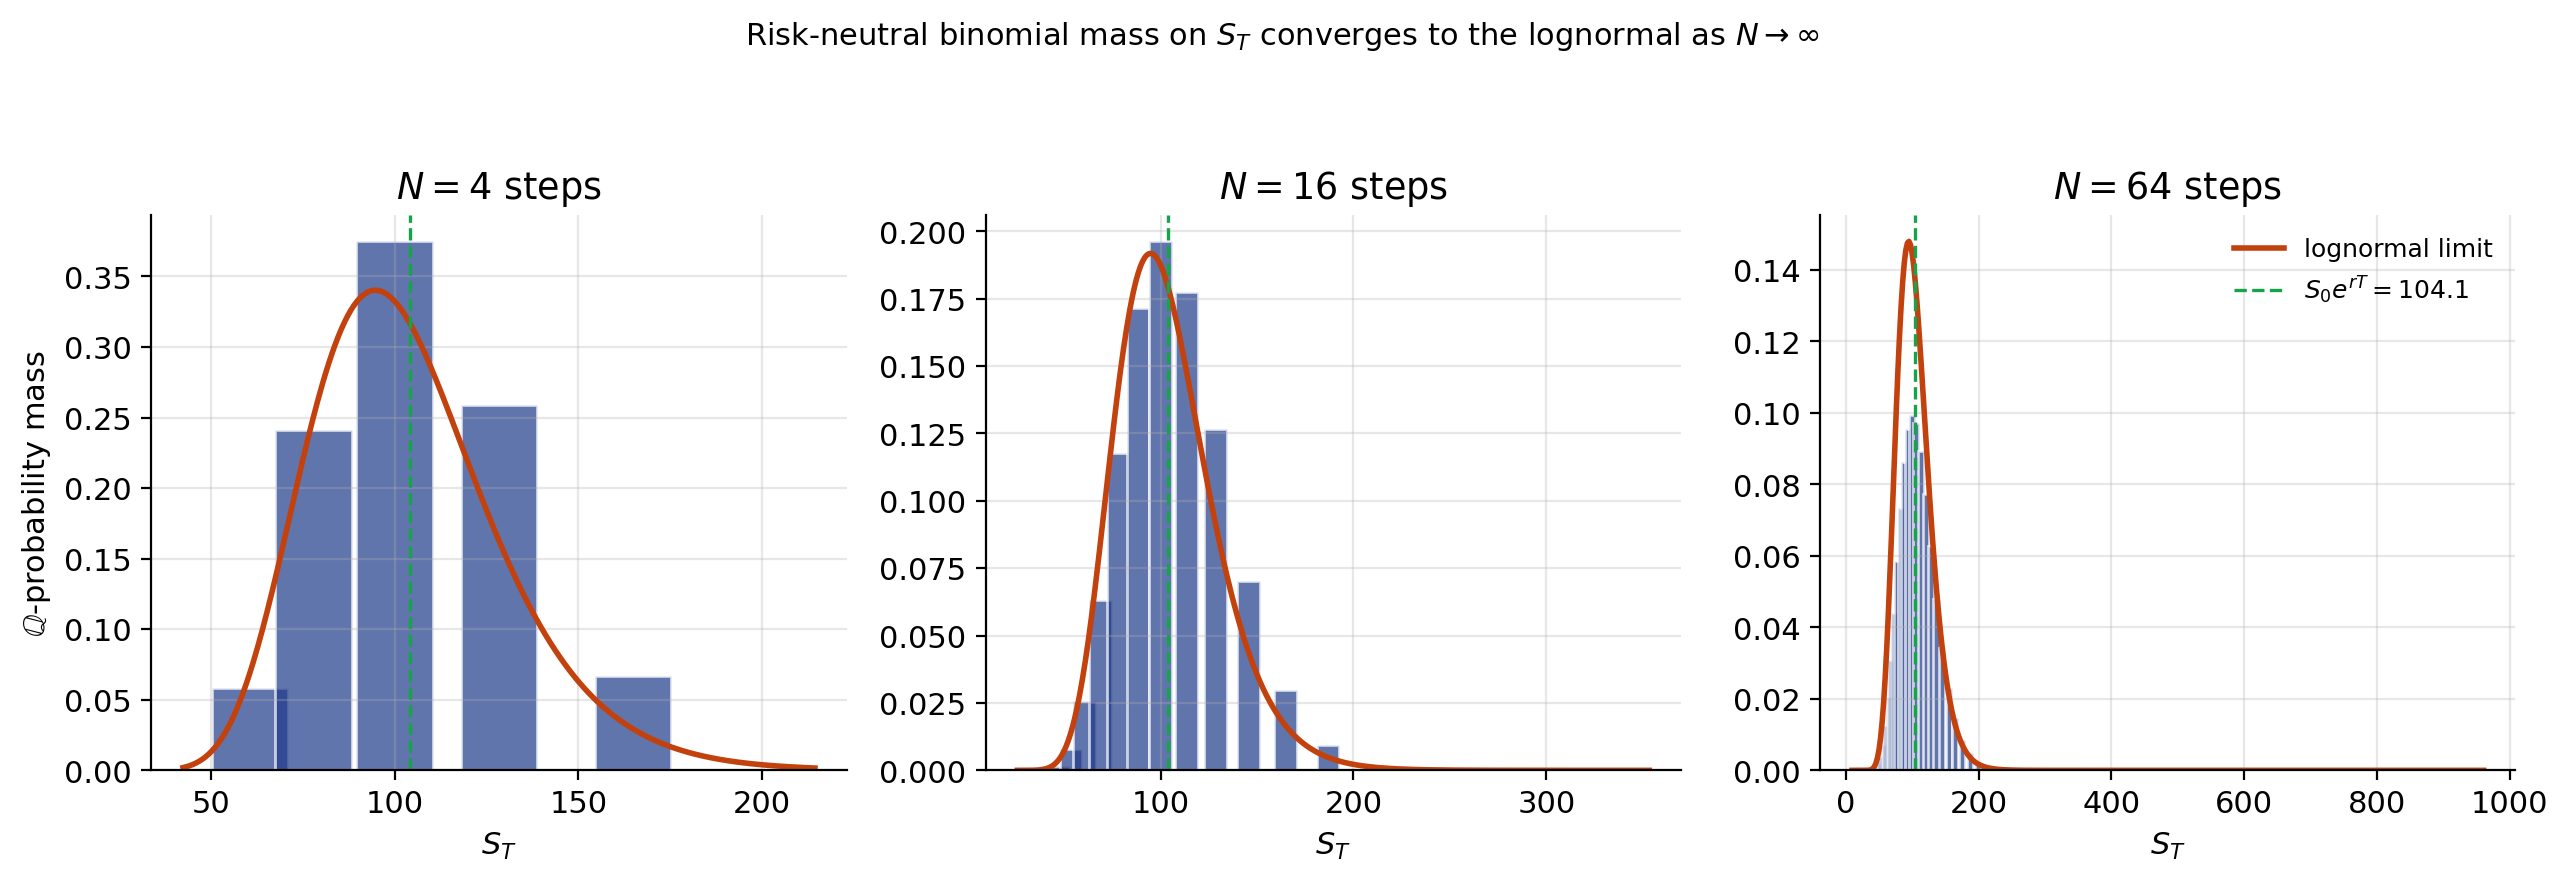
\includegraphics[keepaspectratio]{figures/ch02-rn-measure-evolution.png}}
\caption{Binomial \(\mathbb{Q}\)-mass on \(S_T\) at \(N=4,16,64\) steps,
with the lognormal limiting density overlaid --- the de Moivre-Laplace
CLT in action. The same convergence is why a 252-step daily binomial
tree is indistinguishable from Black-Scholes to within MC noise}
\end{figure}

In words: asset prices in the limit \(N\to\infty\) are lognormal r.v. at
a fixed point in time. Verifying the martingale property under
\(\mathbb{Q}\):

\[\mathbb{E}^{\mathbb{P}}[\,A_T\,] \;=\; A_0\, e^{\mu T}\,\mathbb{E}^{\mathbb{P}}\!\bigl[\,e^{\sigma\sqrt{T}\, Z}\,\bigr] \;=\; A_0\, e^{\mu T}\, e^{\tfrac{1}{2}\sigma^2 T} \;=\; A_0\, e^{(\mu + \tfrac{1}{2}\sigma^2) T}, \tag{2.31}\]

\[\mathbb{E}^{\mathbb{Q}}[\,A_T\,] \;=\; A_0\, e^{(r - \tfrac{1}{2}\sigma^2) T}\, e^{\tfrac{1}{2}\sigma^2 T} \;=\; A_0\, e^{r T}. \tag{2.32}\]

Used: \(\mathbb{E}[e^{\alpha Z}] = e^{\alpha^2/2}\). Under
\(\mathbb{Q}\) the log-return drift is \(r - \tfrac12\sigma^2\) but the
price grows at \(r\) --- Jensen on \(e^X\). In log-normal markets, the
right-tail pulls the mean up by exactly \(\tfrac12\sigma^2\) above the
median.

\subsection{\texorpdfstring{2.3.6 Calibrating to log-returns vs simple
returns --- the \(\tfrac{1}{2}\sigma^2\)
correction}{2.3.6 Calibrating to log-returns vs simple returns --- the \textbackslash tfrac\{1\}\{2\}\textbackslash sigma\^{}2 correction}}\label{calibrating-to-log-returns-vs-simple-returns-the-tfrac12sigma2-correction}

Caveat: if you calibrate \(\mu\) from simple returns
\((S_{m+1} - S_m)/S_m\) instead of log-returns, you over-state the
log-drift by \(\tfrac12\sigma^2\) --- ``volatility drag.'' For the S\&P
500 at \(\sigma = 16\%\), the gap between simple-return \(\mu = 10\%\)
and the compounded growth rate \(\approx 8.7\%\) produces a 40\%
terminal-wealth difference over 30 years. \emph{Always log before
averaging:} compute \(r_m = \ln(S_{m+1}/S_m)\), then take sample mean
and variance.

\subsection{2.3.7 Pricing vanilla European claims in the CRR
limit}\label{pricing-vanilla-european-claims-in-the-crr-limit}

From \(C_0/B_0 = \mathbb{E}^{\mathbb{Q}}[C_T/B_T]\) and (2.30):

\[C_0 \;=\; e^{-rT}\, \mathbb{E}^{\mathbb{Q}}\!\left[\,(A_T - K)_+\,\right], \qquad A_T \;\stackrel{d}{=}\; A_0\, e^{(r - \tfrac{1}{2}\sigma^2)T + \sigma\sqrt{T}\, Z}. \tag{2.34}\]

The integral evaluates to the Black--Scholes formula (sketched in §2.9;
derived in Chapter 6).

\begin{center}\rule{0.5\linewidth}{0.5pt}\end{center}

\section{2.4 The Alternate CRR Parameterisation --- Direct-Gaussian
Increment
Lattice}\label{the-alternate-crr-parameterisation-direct-gaussian-increment-lattice}

The classical CRR pushes drift into the probability \(p\). An equivalent
alternate lattice (essentially Jarrow--Rudd) absorbs the Itô convexity
into the \emph{nodes} and keeps \(p = \tfrac12\). Many discretisations
converge to the same GBM; the choice trades off where the drift
information lives.

\subsection{2.4.1 The two parameterisations, side by
side}\label{the-two-parameterisations-side-by-side}

Parameterisation I --- symmetric nodes, biased probability (§2.3):

\[A \to \begin{cases} A\, e^{+\sigma\sqrt{\Delta t}} & \text{w.p. } p \\[4pt] A\, e^{-\sigma\sqrt{\Delta t}} & \text{w.p. } 1-p \end{cases}, \quad p = \tfrac{1}{2}[1 + \tfrac{\mu}{\sigma}\sqrt{\Delta t}] + \cdots \tag{2.35}\]

Parameterisation II --- drift-shifted nodes, symmetric probability:

\[A \to \begin{cases} A\, e^{(\mu - \tfrac{1}{2}\sigma^2)\Delta t + \sigma\sqrt{\Delta t}} & \text{w.p. } \tfrac{1}{2} \\[4pt] A\, e^{(\mu - \tfrac{1}{2}\sigma^2)\Delta t - \sigma\sqrt{\Delta t}} & \text{w.p. } \tfrac{1}{2} \end{cases} \tag{2.36}\]

\emph{Intuition.} Both converge to the same lognormal GBM.
Parameterisation II is the moment-matched Euler--Maruyama scheme for
log-GBM:
\(X_{n+1} = X_n + (r-\tfrac12\sigma^2)\Delta t + \sigma\cdot\pm\sqrt{\Delta t}\).
It is nicer for Monte Carlo (fair coin), parameterisation I is closer to
the one-step no-arb picture.

\subsection{2.4.2 Verifying parameterisation II matches the first two
log-moments}\label{verifying-parameterisation-ii-matches-the-first-two-log-moments}

Under \(\mathbb{P}\) with \(p = \tfrac{1}{2}\) on tree (2.36):

\[\mathbb{E}^{\mathbb{P}}[A_1] \;=\; A\, e^{(\mu - \tfrac{1}{2}\sigma^2)\Delta t}\cdot \tfrac{1}{2}\!\left[\,e^{+\sigma\sqrt{\Delta t}} + e^{-\sigma\sqrt{\Delta t}}\,\right]. \tag{2.37}\]

Expanding
\(\tfrac{1}{2}[e^{z} + e^{-z}] = 1 + \tfrac{1}{2}z^2 + \cdots\) with
\(z = \sigma\sqrt{\Delta t}\):

\[\mathbb{E}^{\mathbb{P}}[A_1] \;=\; A\, e^{(\mu - \tfrac{1}{2}\sigma^2)\Delta t}\!\left(1 + \tfrac{1}{2}\sigma^2\Delta t + \cdots\right) \;=\; A\, e^{\mu\Delta t} + \cdots, \tag{2.38}\]

matching the target \(\mathbb{E}^{\mathbb{P}}[A_1] = A e^{\mu\Delta t}\)
to the relevant order. The log-variance

\[\mathbb{V}^{\mathbb{P}}[\ln(A_1/A)] \;=\; \sigma^2\,\Delta t \tag{2.39}\]

is exact (not just leading-order) because the
\(\pm\sigma\sqrt{\Delta t}\) Bernoulli has variance \(\sigma^2\Delta t\)
by construction, and the deterministic drift
\((\mu - \tfrac{1}{2}\sigma^2)\Delta t\) drops out of the variance.

\subsection{\texorpdfstring{2.4.3 Risk-neutral probability \(q\) under
parameterisation
II}{2.4.3 Risk-neutral probability q under parameterisation II}}\label{risk-neutral-probability-q-under-parameterisation-ii}

Applying the martingale condition
\(A = e^{-r\Delta t}\mathbb{E}^{\mathbb{Q}}[A_1]\) to tree (2.36) with
\(\mathbb{Q}\)-probabilities \((q, 1-q)\):

\[A \;=\; e^{-r\Delta t}\!\left[\,q\, A\, e^{(\mu - \tfrac{1}{2}\sigma^2)\Delta t + \sigma\sqrt{\Delta t}} \;+\; (1-q)\, A\, e^{(\mu - \tfrac{1}{2}\sigma^2)\Delta t - \sigma\sqrt{\Delta t}}\,\right]. \tag{2.40}\]

Solving for \(q\):

\[q \;=\; \frac{e^{r\Delta t} - e^{(\mu - \tfrac{1}{2}\sigma^2)\Delta t - \sigma\sqrt{\Delta t}}}{e^{(\mu - \tfrac{1}{2}\sigma^2)\Delta t + \sigma\sqrt{\Delta t}} - e^{(\mu - \tfrac{1}{2}\sigma^2)\Delta t - \sigma\sqrt{\Delta t}}} \;=\; \frac{e^{(r - (\mu - \tfrac{1}{2}\sigma^2))\Delta t} - e^{-\sigma\sqrt{\Delta t}}}{e^{+\sigma\sqrt{\Delta t}} - e^{-\sigma\sqrt{\Delta t}}}. \tag{2.41}\]

Introduce the shorthand \(\hat r := r - (\mu - \tfrac{1}{2}\sigma^2)\).
Expanding to \(O(\sqrt{\Delta t})\):

\[q \;\sim\; \frac{(1 + \hat r\Delta t) - (1 - \sigma\sqrt{\Delta t} + \tfrac{1}{2}\sigma^2\Delta t)}{(1 + \sigma\sqrt{\Delta t} + \tfrac{1}{2}\sigma^2\Delta t) - (1 - \sigma\sqrt{\Delta t} + \tfrac{1}{2}\sigma^2\Delta t)} + \cdots \;=\; \frac{\sigma\sqrt{\Delta t} + (\hat r - \tfrac{1}{2}\sigma^2)\Delta t}{2\sigma\sqrt{\Delta t}} + \cdots, \tag{2.42}\]

\[q \;\sim\; \tfrac{1}{2}\!\left[\,1 + \frac{\hat r - \tfrac{1}{2}\sigma^2}{\sigma}\sqrt{\Delta t}\,\right] + \cdots \;=\; \tfrac{1}{2}\!\left[\,1 + \frac{r - \mu}{\sigma}\sqrt{\Delta t}\,\right] + \cdots, \tag{2.43}\]

where the last step uses
\(\hat r - \tfrac{1}{2}\sigma^2 = r - (\mu - \tfrac{1}{2}\sigma^2) - \tfrac{1}{2}\sigma^2 = r - \mu\).

Comparison with classical CRR (2.23):

\[q_{\text{CRR}} \;\sim\; \tfrac{1}{2}\!\left[\,1 + \frac{r - \tfrac{1}{2}\sigma^2}{\sigma}\sqrt{\Delta t}\,\right] + \cdots \tag{2.44}\]

The two \(q\)'s differ at \(O(\sqrt{\Delta t})\) by exactly the physical
drift term, because parameterisation II has already absorbed the drift
\((\mu - \tfrac{1}{2}\sigma^2)\) into the node geometry. In the
continuous-time limit both parameterisations yield the same lognormal
\(A_T\) distribution under \(\mathbb{Q}\) --- consistent with (2.30).

\subsection{2.4.4 Reconciling parameterisations I and
II}\label{reconciling-parameterisations-i-and-ii}

By construction of \(q\) in (2.40) the martingale relation
\(\mathbb{E}^{\mathbb{Q}}[A_1] = A e^{r\Delta t}\) is exact, and
\(\mathbb{V}^{\mathbb{Q}}[\ln(A_1/A)] = \sigma^2\Delta t + O(\Delta t^{3/2})\).
A one-parameter family unifies the two: take node geometry
\(A\,e^{(\alpha - \tfrac12\sigma^2)\Delta t \pm \sigma\sqrt{\Delta t}}\)
with probability
\(p = \tfrac12[1 + (\mu - \alpha)\sqrt{\Delta t}/\sigma] + \cdots\). The
choice \(\alpha = \mu\) recovers parameterisation II (\(p = \tfrac12\));
\(\alpha = 0\) recovers classical CRR. All choices converge to the same
GBM; they only differ in finite-\(\Delta t\) convergence constants. When
comparing two binomial-tree implementations, always check the
parameterisation convention --- a 0.5\% discrepancy at \(N=100\) may
just reflect different \(\alpha\).

\begin{center}\rule{0.5\linewidth}{0.5pt}\end{center}

\section{2.5 The Fundamental Theorem of Asset
Pricing}\label{the-fundamental-theorem-of-asset-pricing}

FTAP. No arbitrage \(\iff\) there exists \(\mathbb{Q} \sim \mathbb{P}\)
such that for every traded asset \(X\), the discounted price
\(\tilde{X}_t = X_t/B_t\) is a \(\mathbb{Q}\)-martingale:

\[\tilde{X}_t \;=\; \mathbb{E}^{\mathbb{Q}}\!\left[\,\tilde{X}_s \mid \mathcal{F}_t\,\right], \qquad s \ge t. \tag{2.48}\]

The physical measure \(\mathbb{P}\) describes how the world evolves;
\(\mathbb{Q}\) re-weights so all tradable risks have zero expected
excess return. Equivalence \(\mathbb{Q} \sim \mathbb{P}\) means
agreement on null sets --- essential, else we could win on a
\(\mathbb{P}\)-non-null event the \(\mathbb{Q}\)-price ignores.

Two flavours: \emph{First FTAP} (no-arb \(\Leftrightarrow\)
\(\mathcal{M}_e \neq \emptyset\)) and \emph{Second FTAP} (completeness
\(\Leftrightarrow\) \(|\mathcal{M}_e| = 1\)). Binomial trees satisfy
both; trinomial trees (or any market with more states than tradables)
satisfy only the first and admit a family of \(\mathbb{Q}\). The
Delbaen--Schachermayer extension to semimartingales replaces ``no
arbitrage'' by ``no free lunch with vanishing risk'' (NFLVR). The
natural numéraire is the money-market account \(B_t = e^{rt}\) but any
strictly positive traded asset works; this freedom is exploited in
Chapter 5.

\begin{figure}
\centering
\pandocbounded{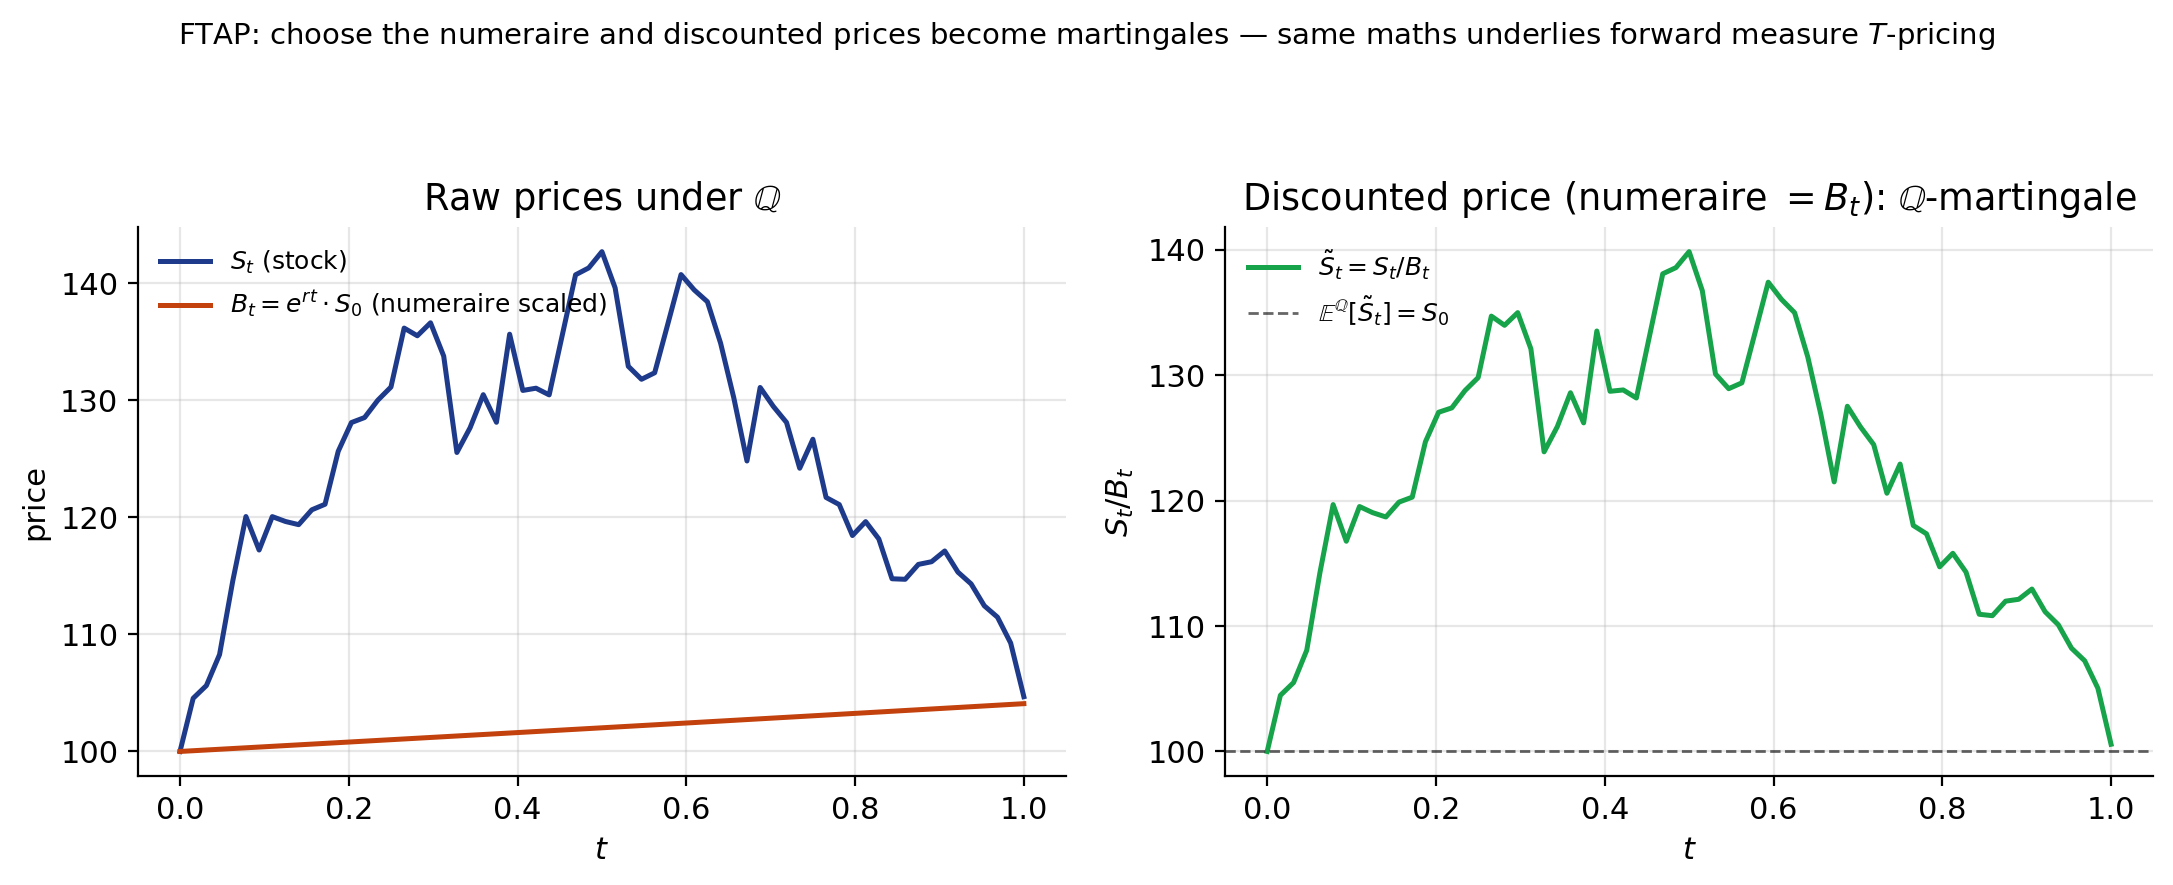
\includegraphics[keepaspectratio]{figures/ch02-numeraire-rebasing.png}}
\caption{Same simulated \(\mathbb{Q}\)-path of \(S_t\): raw price grows
on average at rate \(r\) (left); divided by the numeraire
\(B_t = e^{rt}\) the discounted price is a \(\mathbb{Q}\)-martingale
(right). Numeraire freedom underlies forward-measure pricing of caplets
and bond options}
\end{figure}

\begin{center}\rule{0.5\linewidth}{0.5pt}\end{center}

\section{2.6 Non-Uniqueness of the Martingale
Measure}\label{non-uniqueness-of-the-martingale-measure}

The binomial tree's completeness is an artefact of the lattice. Real
markets have far more states than tradable instruments --- jumps,
stoch-vol, default, liquidity freezes --- and any one of these creates
an un-spanned payoff. In the one-step binomial \(\mathbb{Q}\) was pinned
down by one linear equation in one unknown \(q\); once the underlying
branches to three or more states, \(\mathbb{Q}\) is no longer unique.
The FTAP still holds; \(\mathcal{M}_e\) is non-empty but not a
singleton.

Selecting a single price from the arbitrage-free interval is what the
calibration industry does: fitting \(\mathbb{Q}\) to liquid benchmark
instruments (vanilla options, CDS), utility-based criteria, or robust
pricing under ambiguity each pick a representative element of
\(\mathcal{M}_e\).

Why three post-states destroys uniqueness: each tradable adds one linear
constraint \(\mathbb{E}^{\mathbb{Q}}[X_1] = X_0 e^{r\Delta t}\), while
an \(n\)-state probability vector has \(n-1\) free coordinates. For
\(n = k\) tradables, the system is exactly determined; for \(k < n\),
\(\mathcal{M}_e\) is \((n-k)\)-dimensional. Adding tradables (e.g.~index
options) restores uniqueness --- this is the
\emph{calibration-to-market} strategy that dominates quant practice.

We have two martingale equations (for cash and the stock) but three or
four unknown probabilities, so

\[\mathbb{Q} \text{ is not unique} \;\Longrightarrow\; C_0 \text{ is not necessarily unique.} \tag{2.50}\]

In incomplete markets the price spans an \emph{arbitrage-free interval}:
from the super-replication cost (cheapest dominating portfolio) to the
sub-replication value. The market-clearing price within this interval
depends on risk preferences, hedging technology, and supply--demand.

\pandocbounded{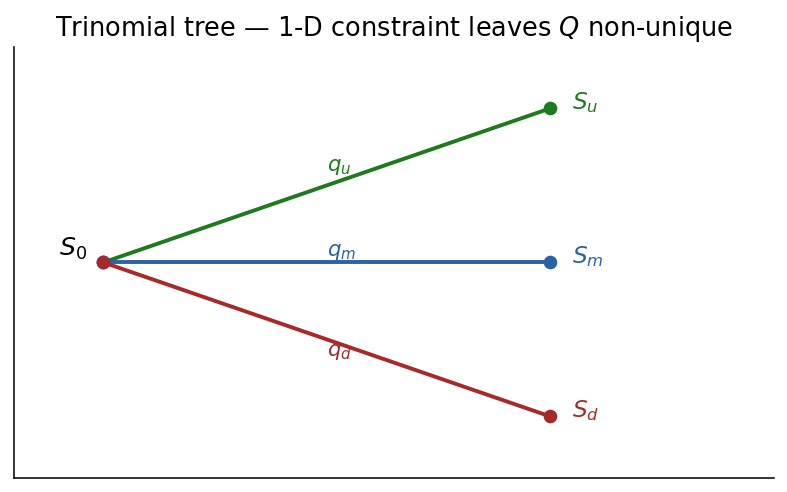
\includegraphics[keepaspectratio]{figures/ch02-trinomial.png}}
\emph{Trinomial tree --- non-uniqueness of Q}

\subsection{2.6.1 Geometric picture and local
risk-minimisation}\label{geometric-picture-and-local-risk-minimisation}

Tradable assets span a \emph{replicable subspace} of payoff space. A
claim in the subspace has a unique price; a claim outside requires a
selection criterion. \emph{Local risk-minimisation} projects the claim
onto the subspace under \(L^2(\mathbb{P})\):

\[C_0 \text{ is unique iff the claim lies in } \operatorname{span}(A_1, B_1), \qquad \min_{(\alpha,\beta)}\,\mathbb{E}^{\mathbb{P}}[(\alpha A_1 + \beta B_1 - C_1)^2]. \tag{2.51–2.52}\]

The foot of the perpendicular is the optimal static hedge; its length is
the unhedgeable residual standard deviation. Other rules ---
minimum-entropy, minimum-variance, Esscher, utility indifference ---
pick different elements of \(\mathcal{M}_e\).

\emph{Worked.} Trinomial \(S_0 = 10\), \(S_1 \in \{12, 10, 8\}\),
\(p = (1/3, 1/3, 1/3)\), \(r = 0\), call \(C_1 = (2, 0, 0)\). Projecting
onto \(\operatorname{span}(\mathbf{1}, S_1)\):
\(\beta^\star = (4/3)/(8/3) = 1/2\), \(\alpha^\star = -14/3\), residual
variance \(1/3\). The arbitrage-free interval is \((0, 1)\).

\begin{center}\rule{0.5\linewidth}{0.5pt}\end{center}

\section{2.7 Default Model and Incomplete-Market
Trees}\label{default-model-and-incomplete-market-trees}

We build a discrete default model that converges to a diffusion with a
jump to zero --- our first concrete incomplete-market tree. Default is a
\emph{jump process}: rare, catastrophic, discrete. The mathematical
framework is a Poisson point process with intensity \(\hat\lambda\), the
expected rate of jumps per unit time. With three states
(up/down/default) and only two tradables (stock, cash),
\(\mathcal{M}_e\) has dimension one --- calibrate \(\hat\lambda\) from
CDS spreads or corporate bond yields.

The physical intensity \(\lambda\) is generally lower than the
risk-neutral \(\hat\lambda\); the gap is the credit risk premium (for IG
issuers, \(\hat\lambda\) is 2--5x \(\lambda\)).

On \([t, t+\Delta t]\):

\[A_n = A_{n-1} \, e^{\sigma \sqrt{\Delta t}\, x_n}, \qquad p = \tfrac12[1 + (\mu - \tfrac12\sigma^2)\sqrt{\Delta t}/\sigma]. \tag{2.53}\]

Lifetime \(\tau \sim \text{Exp}(\hat\lambda)\). One-step default
probability:

\[\mathbb{P}(\tau \in (t, t+\Delta t] | \tau > t) = 1 - e^{-\hat\lambda\Delta t} \approx \hat\lambda\,\Delta t. \tag{2.54}\]

Memorylessness
(\(\mathbb{P}(\tau > t+s | \tau > s) = \mathbb{P}(\tau > t)\)) is the
defining feature of the exponential. Empirically wrong (default
intensities cluster in time, firms have age effects), but pedagogically
clean --- Cox/doubly-stochastic processes generalise. Typical IG
corporate intensities: \(\hat\lambda \in [0.005, 0.015]\)/yr; HY:
\([0.05, 0.20]\)/yr.

\subsection{2.7.1 Branching tree with default
branch}\label{branching-tree-with-default-branch}

From a pre-default node \(A_{n-1}\) the tree has three children:

\[A_{n-1} \longrightarrow \begin{cases} A_{n-1}\, e^{+\sigma\sqrt{\Delta t}} & \text{w.p. } p\,(1 - \hat{\lambda}\Delta t) \\[4pt] A_{n-1}\, e^{-\sigma\sqrt{\Delta t}} & \text{w.p. } (1-p)(1 - \hat{\lambda}\Delta t) \\[4pt] 0 & \text{w.p. } \hat{\lambda}\,\Delta t \end{cases} \tag{2.55}\]

The riskless bond pays \(e^{r\Delta t}\) in all three states; the risky
asset jumps to \(0\) on default --- the tree is binomial conditional on
survival, with a third ray to zero.

\subsection{2.7.2 Survival law}\label{survival-law}

For \(\tau \sim \text{Exp}(\hat\lambda)\):
\(\mathbb{P}(\tau > T) = e^{-\hat\lambda T}\), density
\(f_\tau(t) = \hat\lambda e^{-\hat\lambda t}\), mean \(1/\hat\lambda\).
At \(\hat\lambda = 5\%\): 5-yr survival \(\approx 77.9\%\), 10-yr
\(\approx 60.7\%\), mean default time 20 years. Time-varying intensity
\(\hat\lambda(t)\) generalises to \(\exp(-\int_0^T \hat\lambda(s)ds)\).

\subsection{\texorpdfstring{2.7.3 Risk-neutral \(q\) --- default-free
sub-case}{2.7.3 Risk-neutral q --- default-free sub-case}}\label{risk-neutral-q-default-free-sub-case}

Setting \(\hat\lambda = 0\) recovers (2.22):
\(q = (e^{r\Delta t} - e^{-\sigma\sqrt{\Delta t}})/(e^{\sigma\sqrt{\Delta t}} - e^{-\sigma\sqrt{\Delta t}}) \sim \tfrac12[1 + (r-\tfrac12\sigma^2)\sqrt{\Delta t}/\sigma]\)
--- same as before; \(\hat\lambda\) is the \(\mathbb{Q}\)-hazard rate.

\subsection{2.7.4 Including default into the martingale
condition}\label{including-default-into-the-martingale-condition}

The three-branch martingale condition:

\[1 \;=\; q\,(1 - \hat{\lambda}\Delta t)\, e^{\sigma\sqrt{\Delta t} - r\Delta t} \;+\; (1-q)(1 - \hat{\lambda}\Delta t)\, e^{-\sigma\sqrt{\Delta t} - r\Delta t} \;+\; 0 \cdot \hat{\lambda}\Delta t. \tag{2.59}\]

Solving for \(q\):

\[q \;=\; \frac{e^{(r+\hat{\lambda})\Delta t} - e^{-\sigma\sqrt{\Delta t}}}{e^{+\sigma\sqrt{\Delta t}} - e^{-\sigma\sqrt{\Delta t}}} \;\sim\; \tfrac{1}{2}\!\left(1 + \frac{r + \hat{\lambda} - \tfrac{1}{2}\sigma^2}{\sigma}\sqrt{\Delta t}\right) + o(\sqrt{\Delta t}). \tag{2.60}\]

The effect of adding a default branch is therefore to shift the
risk-neutral drift upward by \(\hat{\lambda}\): the surviving branch
must grow faster to compensate for the chance of being wiped out.

\emph{Intuition.} If a fraction \(\hat{\lambda}\Delta t\) of your
probability mass leaks to zero every step, the conditional expected
growth of the survivors has to be higher just to keep the unconditional
expectation at \(e^{r\Delta t}\). Credit risk premia in corporate bonds
have exactly this structure: the yield-to-maturity exceeds the riskless
rate by roughly the expected loss rate
\(\hat{\lambda}\cdot \text{LGD}\).

A concrete credit-pricing illustration. Consider a zero-recovery
one-year zero-coupon bond issued by a firm with default intensity
\(\hat{\lambda} = 3\%\). Its fair price is
\(e^{-(r+\hat{\lambda})T} = e^{-(0.05+0.03)\cdot 1} \approx 0.923\),
compared to the riskless bond price \(e^{-rT}\approx 0.951\). The yield
spread is therefore \(\hat{\lambda} = 3\%\) --- the spread is the
risk-neutral default intensity (in the zero-recovery case). With
recovery \(R\) (so loss-given-default is \(1-R\)), the bond price is
\(e^{-rT}(e^{-\hat{\lambda}T} + R(1-e^{-\hat{\lambda}T}))\approx e^{-rT}(1 - (1-R)\hat{\lambda} T)\),
and the spread is \(\hat{\lambda}(1-R)\) to leading order. This is the
``spread \(=\) probability \(\times\) loss'' relationship that sits at
the heart of the CDS market. The CDS premium quoted by a market-maker
\emph{is} the market-implied \(\hat{\lambda}(1-R)\), and working back
out the probability requires an LGD assumption (typically
\(R\approx 40\%\) for senior unsecured corporate, so \(1-R=60\%\)).

Now bring the stock back into the picture. On our default tree, the
stock's surviving-branch growth is \(e^{(r+\hat{\lambda})\Delta t}\);
its unconditional expectation is \(e^{r\Delta t}\) because the
\(\hat{\lambda}\) leak balances the surviving boost. Stockholders --- as
residual claimants --- bear the full loss on default, so the stock's
equity risk premium under \(\mathbb{Q}\) is pushed upward by the credit
component. Equity traders often combine this with Merton's structural
credit model: view the firm's equity as a call option on its assets,
with strike at the debt's face value. The equity is thus
\emph{naturally} a credit-contingent claim, and the same
\(\hat{\lambda}\) that shows up in debt pricing also shows up in the
equity vol surface (high equity vol goes with high credit spreads). The
stylised empirical fact is sometimes called the ``credit--equity link''.

\subsection{2.7.5 Risk-neutral expectations of
survival}\label{risk-neutral-expectations-of-survival}

Under \(\mathbb{Q}\) the asset and its discounted version satisfy

\[\mathbb{E}^{\mathbb{Q}}\!\left[A_T \; \mathbf{1}_{\{\tau > T\}}\right] \;=\; A_0\, e^{(r+\hat{\lambda})T}, \tag{2.61}\]

and for the bond-denominated (default-insensitive) notional,

\[\mathbb{E}^{\mathbb{Q}}\!\left[A_T\right] \;=\; A_0\, e^{rT}. \tag{2.62}\]

\emph{Intuition.} Equation (2.62) is the FTAP itself at the horizon: the
unconditional expected terminal asset price grows at \(r\). Equation
(2.61) says that, \emph{conditional on surviving}, the asset grows at
the higher rate \(r+\hat{\lambda}\). Taking the product with the
survival probability \(e^{-\hat{\lambda}T}\) recovers (2.62):
\(e^{(r+\hat{\lambda})T}\cdot e^{-\hat{\lambda}T} = e^{rT}\).

\subsection{2.7.6 European pricing recursion with
default}\label{european-pricing-recursion-with-default}

The backward recursion weights all three branches --- up survival, down
survival, default --- by their risk-neutral probabilities. Let
\(C_{n,j}\) denote the option value at node \((n, j)\):

\[\frac{C_{n-1,j}}{B_{n-1}} \;=\; \mathbb{E}^{\mathbb{Q}}\!\left[\frac{C_n}{B_n}\right], \tag{2.63}\]

\[C_{n-1, j} \;=\; q\, \frac{e^{-\hat{\lambda}\Delta t}}{e^{r\Delta t}}\, C_{n, j} \;+\; (1-q)\, \frac{e^{-\hat{\lambda}\Delta t}}{e^{r\Delta t}}\, C_{n, j+1} \;+\; (1 - e^{-\hat{\lambda}\Delta t})\cdot C_{n, d}, \tag{2.64}\]

where the default node satisfies

\[C_{n-1, d} \;=\; C_{n, d}\, e^{-r\Delta t}. \tag{2.65}\]

(On default the stock is \(0\), so a call has \(C_{n,d} \equiv 0\); a
put has \(C_{n,d} = K\) discounted to today.)

\emph{Intuition.} The recursion is the classical binomial backward sweep
with two modifications: each surviving branch is down-weighted by the
survival factor \(e^{-\hat{\lambda}\Delta t}\), and a third term
captures what the option is worth \emph{in} default. For a vanilla call
that third term is zero, so credit risk eats value monotonically; for a
put it is positive (the put still pays on bankruptcy unless it is a
``protected put'' that voids on the issuer's own default).

Numerical: vanilla 1-year ATM call, \(A_0 = K = 100\),
\(\sigma = 20\%\), \(r = 5\%\), \(\hat{\lambda} = 2\%\). Black--Scholes
(no default) gives \(\approx 10.45\); survival-discounted,
\(10.45 \cdot e^{-0.02} \approx 10.24\). A constant default intensity
scales call prices by \(e^{-\hat{\lambda}(T-t)}\) to leading order ---
the standard parameterisation of jump-to-default models.

\begin{center}\rule{0.5\linewidth}{0.5pt}\end{center}

\section{2.8 American Valuation on the Binomial
Tree}\label{american-valuation-on-the-binomial-tree}

US single-stock equity options are American; index options (SPX, RUT)
are European. American exercise lets the holder choose any stopping time
\(\tau \le T\) --- a random time adapted to the filtration
(\(\{\tau \le t\} \in \mathcal{F}_t\), no peeking). The set of stopping
times is combinatorially vast, but Bellman's principle reduces the
problem to a one-line recursion: at each node, take the max of intrinsic
value and continuation value. The recursion runs backward in \(O(N^2)\),
and the exercise boundary is the locus where the max is achieved by
exercising.

\subsection{\texorpdfstring{2.8.1 European \(\to\) American
contrast}{2.8.1 European \textbackslash to American contrast}}\label{european-to-american-contrast}

European pays \(\varphi(A_T)\) at fixed \(T\):

\[V_t \;=\; e^{-r(T - t)}\,\mathbb{E}^{\mathbb{Q}}\!\left[\,\varphi(A_T)\,\right] \;\longrightarrow\; V_T \;=\; \varphi(A_T). \tag{2.66}\]

American option lets the holder choose the exercise epoch \(\tau\), a
stopping time bounded above by \(T\), and pays \(\varphi(A_\tau)\) at
\(\tau\) --- meaning the holder ``receives \(\varphi(A_\tau)\) at the
moment they decide to stop''.

American put, in particular:

\[\varphi(A_\tau) \;=\; (K - A_\tau)_+. \tag{2.67}\]

Let \(\mathcal{S}\) denote the set of \(\{\mathcal{F}_t\}\)-stopping
times bounded by \(T\). Then

\[\frac{C_0}{B_0} \;=\; \sup_{\tau \in \mathcal{S}}\; \mathbb{E}^{\mathbb{Q}}\!\left[\frac{(K - A_\tau)_+}{B_\tau}\right]. \tag{2.68}\]

\emph{Intuition.} The American price is the Snell envelope of the
intrinsic process --- the smallest \(\mathbb{Q}\)-supermartingale
dominating immediate exercise. The optimal stopping time is
\(\tau^* = \inf\{t : V_t = I_t\}\), the first hitting time of the
exercise region. On the lattice this collapses to: at each node
\(V_{n,k} = \max(I_{n,k}, V^h_{n,k})\).

\subsection{2.8.2 Tree diagram --- hold vs
exercise}\label{tree-diagram-hold-vs-exercise}

At every interior node there are two candidate values:

\begin{itemize}
\tightlist
\item
  \(P^h\) --- the hold/continuation value (from the one-step backward
  recursion),
\item
  \(P^x \equiv (K - A)_+\) --- the immediate-exercise (intrinsic) value.
\end{itemize}

The actual American value is \(P = \max(P^h, P^x)\).

\begin{figure}
\centering
\pandocbounded{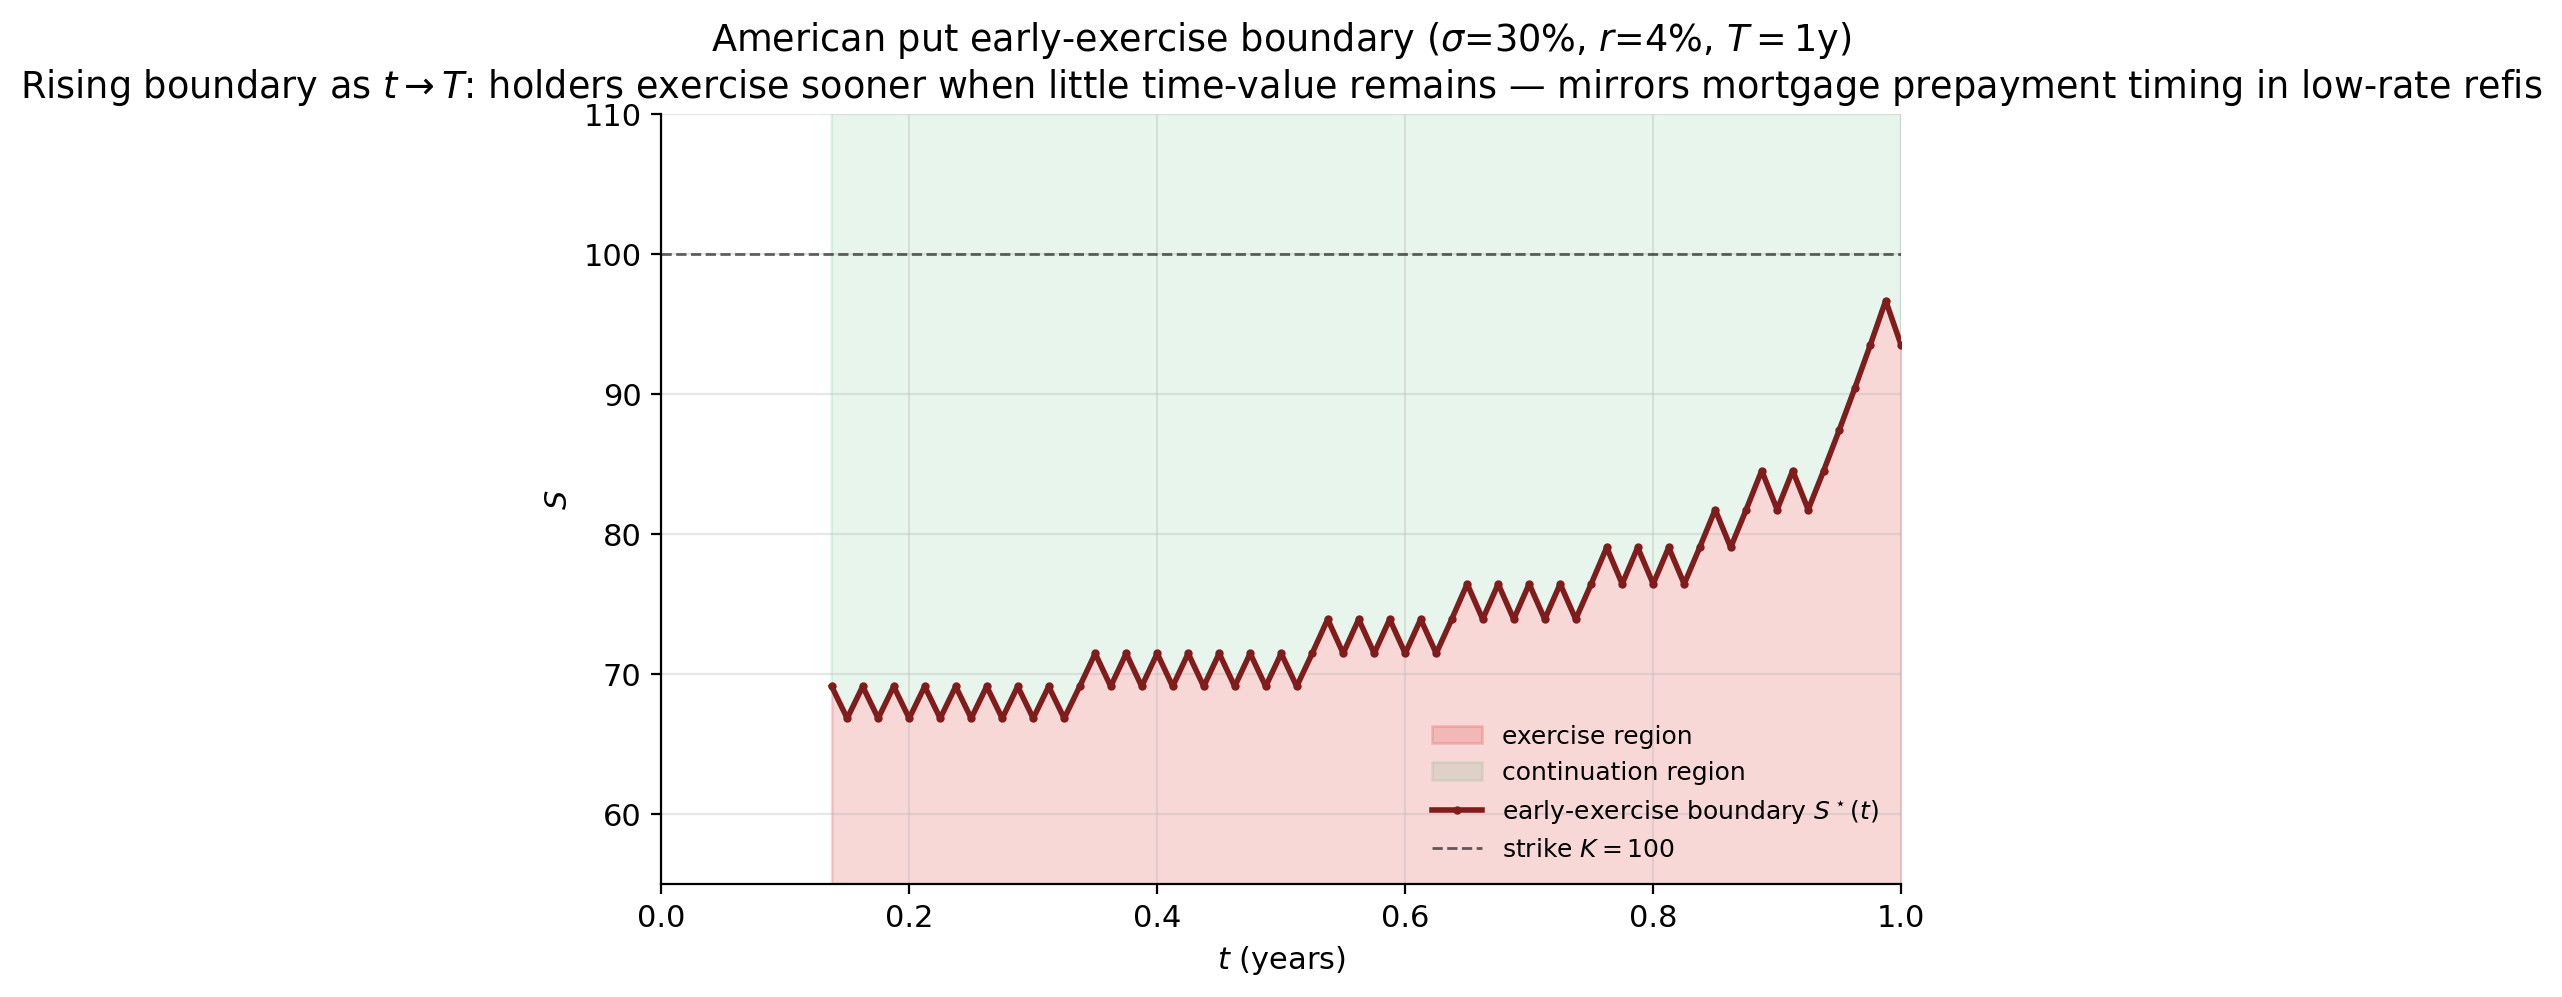
\includegraphics[keepaspectratio]{figures/ch02-american-boundary.png}}
\caption{American put early-exercise boundary \(S^\star(t)\) computed by
CRR backward induction (80 steps, \(\sigma=30\%\), \(r=4\%\), \(T=1\)y):
below the boundary the holder exercises immediately (red region); above
it they hold (green). The same shape appears in mortgage prepayment
modelling --- homeowners refinance once rates drop far enough below the
contract coupon}
\end{figure}

\subsection{2.8.3 Dynamic-programming
recursion}\label{dynamic-programming-recursion}

On a recombining tree with nodes \((n, k)\), propagate two quantities
backward:

\begin{itemize}
\tightlist
\item
  Continuation (holding) value \(C^{h}_{n-1, k}\):
\end{itemize}

\[\frac{C^{h}_{n-1, k}}{B_{n-1, k}} \;=\; q\, \frac{C_{n, k}}{B_{n, k}} \;+\; (1-q)\, \frac{C_{n, k+1}}{B_{n, k+1}} \tag{2.69}\]

\[\Longrightarrow\; C^{h}_{n-1, k} \;=\; e^{-r\Delta t}\,\big(\,q\, C_{n, k} \;+\; (1-q)\, C_{n, k+1}\,\big). \tag{2.70}\]

\begin{itemize}
\tightlist
\item
  Intrinsic (immediate exercise) value \(C^{I}_{n-1, k}\):
\end{itemize}

\[C^{I}_{n-1, k} \;=\; (A_{n-1, k} - K)_+ \quad\text{(call)}, \qquad C^{I}_{n-1, k} \;=\; (K - A_{n-1, k})_+ \quad\text{(put)}. \tag{2.71}\]

\begin{itemize}
\tightlist
\item
  American value --- take the larger:
\end{itemize}

\[\boxed{\; C_{n-1, k} \;=\; \max\!\left(\,C^{I}_{n-1, k},\; C^{h}_{n-1, k}\,\right) \;} \tag{2.72}\]

\subsection{2.8.4 Exercise boundary
picture}\label{exercise-boundary-picture}

The exercise boundary is a free boundary: \(A^*(t)\) is the underlying
value at which the American option equals its intrinsic value,
determined implicitly by the recursion. For an American put
\(A^*(t) < K\) and rises toward \(K\) as \(t \to T\). For an American
call on a dividend-paying stock \(A^*(t) > K\) and falls toward \(K\)
near ex-div.

\emph{Intuition.} For an American put on a non-dividend-payer, early
exercise is driven by interest on the cash proceeds: when the stock
crashes deep enough, \(rK\) outweighs remaining optionality. For an
American call on a non-dividend-payer the boundary never bites --- early
exercise is suboptimal (Merton's theorem). The proof is one inequality:
\(C_t \ge A_t - K e^{-r(T-t)} > A_t - K\), so selling the call always
dominates exercising. The argument fails on a dividend-paying stock
around ex-div, where capturing the cum-dividend price can beat the
post-dividend hold.

The American-put early-exercise premium (AEP) is the gap between
American and European puts. At \(S_0 = K = 100\), \(\sigma = 20\%\),
\(r = 5\%\), \(T = 1\), AEP is a few cents, growing with moneyness,
rate, and maturity. No closed form; binomial or Longstaff--Schwartz
regression is standard.

\pandocbounded{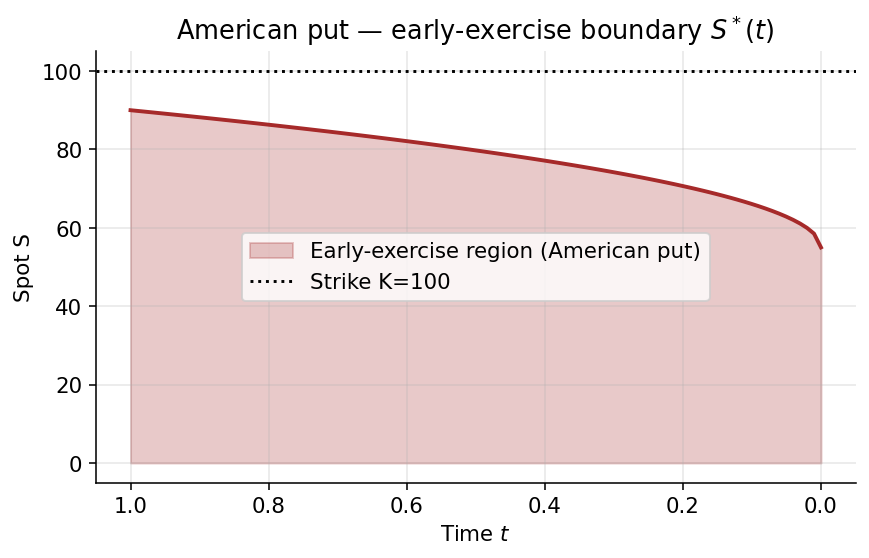
\includegraphics[keepaspectratio]{figures/ch02-american-exercise.png}}
\emph{American put early-exercise boundary}

\begin{center}\rule{0.5\linewidth}{0.5pt}\end{center}

\section{2.9 Bridge to Continuous Time}\label{bridge-to-continuous-time}

The CRR lattice converged via the CLT to a lognormal \(A_T\):

\[A_T \;\stackrel{d}{=}\; A_0\, e^{(r - \tfrac{1}{2}\sigma^2)T \;+\; \sigma\sqrt{T}\, Z_{\mathbb{Q}}}, \qquad Z_{\mathbb{Q}} \sim \mathcal{N}(0, 1). \tag{2.73}\]

That is the marginal at maturity. To upgrade to a \emph{process}, take
the scaled sum of Bernoulli shocks,

\[W^N_t \;:=\; \sqrt{\Delta t}\sum_{n=1}^{\lfloor t/\Delta t\rfloor} x_n, \tag{2.74}\]

which converges in distribution (Donsker's functional CLT) to Brownian
motion \(W_t\). The asset converges to geometric Brownian motion under
\(\mathbb{Q}\):

\[A_t \;=\; A_0\, e^{(r - \tfrac{1}{2}\sigma^2)t \;+\; \sigma W_t}, \qquad dA_t \;=\; r\,A_t\,dt \;+\; \sigma\,A_t\,dW_t. \tag{2.75}\]

Rigorous derivation needs Brownian motion, the stochastic integral, and
Itô's lemma --- all built in Ch. 3.

The European call in the GBM limit is the Black--Scholes formula,

\[C_0 \;=\; A_0\,\Phi(d_+) \;-\; K\,e^{-rT}\,\Phi(d_-), \qquad d_\pm \;=\; \frac{\ln(A_0/K) + (r \pm \tfrac{1}{2}\sigma^2)T}{\sigma\sqrt{T}}, \tag{2.76}\]

derived directly via the measure-change split
\((A_T - K)_+ = A_T \mathbf{1}_{\{A_T > K\}} - K \mathbf{1}_{\{A_T > K\}}\),
pricing each piece under its natural numéraire (stock vs cash) and
reading the exceedance probabilities as Gaussian tails. The same formula
drops out of the Ch. 6 hedging argument once Itô is available.

Three takeaways from this chapter:

\begin{enumerate}
\def\labelenumi{\arabic{enumi}.}
\tightlist
\item
  The no-arbitrage price of any European claim is a discounted
  \(\mathbb{Q}\)-expectation of its payoff.
\item
  Backward induction makes the expectation \(O(N^2)\) and extends to
  American exercise.
\item
  In the limit the tree becomes GBM and vanilla Euros become
  Black--Scholes --- pinned down rigorously in Ch. 3--6.
\end{enumerate}

\begin{center}\rule{0.5\linewidth}{0.5pt}\end{center}

\section{Key Takeaways}\label{key-takeaways-1}

\begin{enumerate}
\def\labelenumi{\arabic{enumi}.}
\tightlist
\item
  The one-period no-arb inequality \(A_d < A(1 + r) < A_u\) is
  equivalent to existence of a risk-neutral measure \(\mathbb{Q}\) such
  that \(C = (1+r)^{-1}\mathbb{E}^{\mathbb{Q}}[C_1]\).
\item
  Multi-period backward induction prices any European payoff via
  repeated one-step discounted risk-neutral expectations --- the
  tower-property manifestation of
  \(C_0 = \mathbb{E}^{\mathbb{Q}}[e^{-rT}C_T]\).
\item
  Classical CRR calibration. Match two moments of the log-return:
  \(c = \sigma\sqrt{\Delta t}\),
  \(p = \tfrac{1}{2}(1 + \tfrac{\mu}{\sigma}\sqrt{\Delta t})\); the
  risk-neutral
  \(q = \tfrac{1}{2}(1 + \tfrac{r - \sigma^2/2}{\sigma}\sqrt{\Delta t})\).
\item
  Alternate CRR (drift-shifted lattice). Nodes
  \(A\cdot e^{(\mu - \tfrac{1}{2}\sigma^2)\Delta t \pm \sigma\sqrt{\Delta t}}\)
  with symmetric probability \(p = \tfrac{1}{2}\); the Itô correction is
  baked into the geometry. Under \(\mathbb{Q}\),
  \(q \sim \tfrac{1}{2}[1 + \tfrac{r - \mu}{\sigma}\sqrt{\Delta t}]\).
  Both parameterisations converge to the same lognormal GBM.
\item
  Measure-invariant variance.
  \(\mathbb{V}^{\mathbb{P}}[\ln A_T] = \mathbb{V}^{\mathbb{Q}}[\ln A_T] = \sigma^2 T\)
  --- Girsanov cannot change volatility, only drift.
\item
  Simple- vs log-return bias. Fitting to simple returns shifts the drift
  estimate by \(+\tfrac{1}{2}\sigma^2\); always be explicit which object
  is being fit.
\item
  FTAP equates no-arbitrage to the existence of an equivalent martingale
  measure \(\mathbb{Q}\) under which all discounted traded assets are
  \(\mathbb{Q}\)-martingales.
\item
  Numéraire freedom. Any strictly positive traded asset \(B_t\) can
  discount --- picking \(B_t\) is picking a measure. Canonical
  derivation of the change-of-measure mechanics is deferred to Chapter
  5.
\item
  Non-uniqueness of \(\mathbb{Q}\) appears as soon as the number of
  future states exceeds the number of traded assets: the claim may not
  lie in \(\operatorname{span}(A_1, B_1)\). The set \(\mathcal{M}_e\) of
  equivalent martingale measures has dimension \(n-k\) for \(n\) states
  and \(k\) tradables.
\item
  Local risk-minimisation
  \(\min_{\alpha,\beta}\mathbb{E}^{\mathbb{P}}[(\alpha A_1 + \beta B_1 - C_1)^2]\)
  selects a hedge but leaves residual, unhedgeable variance.
\item
  Default as a third branch adds the probability mass
  \(\hat{\lambda}\Delta t\) at \(0\) and shifts the risk-neutral drift
  by \(+\hat{\lambda}\) --- the surviving branch must grow faster to
  compensate. This is our first concrete incomplete-market tree.
\item
  Binomial-to-GBM limit. With Bernoulli \(\pm 1\) increments under
  \(\mathbb{Q}\),
  \(A_T \xrightarrow{d} A_0\, e^{(r - \tfrac{1}{2}\sigma^2)T + \sigma\sqrt{T} Z}\)
  --- the marginal distribution of geometric Brownian motion.
\item
  Donsker's functional CLT promotes the scaled random walk of the
  log-price to a Brownian motion \(W_t\) on \([0,T]\), giving GBM
  \(dA_t = rA_t\,dt + \sigma A_t\,dW_t\) --- deferred to Chapter 3 for
  the rigorous construction.
\item
  Black--Scholes \(C_0 = A_0\Phi(d_+) - Ke^{-rT}\Phi(d_-)\) is the
  CRR-limit pricing formula for a European call. The derivation via
  measure change and Itô's lemma is given in Chapters 5 and 6.
\item
  American options require pointwise comparison of intrinsic and holding
  values at every node; the optimal policy is a stopping time defined by
  the exercise boundary. American calls on non-dividend-paying stock
  equal European calls (Merton's theorem); American puts have a strictly
  positive early-exercise premium.
\item
  Monte-Carlo simulation and path-dependent options (cliquets, barriers,
  Asians) are treated in Chapter 9, once the GBM path generator has been
  placed on rigorous footing in Chapter 3.
\end{enumerate}

\begin{center}\rule{0.5\linewidth}{0.5pt}\end{center}

\section{Reference Formulas}\label{reference-formulas-1}

One-period no-arbitrage.
\[A_d < A(1 + r) < A_u \;\iff\; \exists\,\mathbb{Q}\text{ s.t. } C = \tfrac{1}{1+r}\,\mathbb{E}^{\mathbb{Q}}[C_1].\]

FTAP / discounted martingale.
\[\tilde{X}_t = \frac{X_t}{B_t}, \qquad \tilde{X}_t = \mathbb{E}^{\mathbb{Q}}\!\left[\tilde{X}_s \mid \mathcal{F}_t\right].\]

Classical CRR calibration (moment-matching).
\[c \;\sim\; \sigma\sqrt{\Delta t}, \qquad p \;\sim\; \tfrac{1}{2}\!\left(1 + \tfrac{\mu}{\sigma}\sqrt{\Delta t}\right), \qquad q \;\sim\; \tfrac{1}{2}\!\left(1 + \tfrac{r - \tfrac{1}{2}\sigma^2}{\sigma}\sqrt{\Delta t}\right).\]

Alternate CRR (drift-shifted lattice).
\[A \to A\, e^{(\mu - \tfrac{1}{2}\sigma^2)\Delta t \pm \sigma\sqrt{\Delta t}}, \qquad p = \tfrac{1}{2}, \qquad q \;\sim\; \tfrac{1}{2}\!\left[\,1 + \tfrac{r - \mu}{\sigma}\sqrt{\Delta t}\,\right] + \cdots.\]

Log-moment invariance.
\[\mathbb{E}^{\mathbb{P}}[\ln(A_T/A_0)] = \mu T, \qquad \mathbb{E}^{\mathbb{Q}}[\ln(A_T/A_0)] = (r - \tfrac{1}{2}\sigma^2) T, \qquad \mathbb{V}^{\mathbb{P}}[\ln(A_T/A_0)] = \mathbb{V}^{\mathbb{Q}}[\ln(A_T/A_0)] = \sigma^2 T.\]

Local risk-minimising hedge.
\[\min_{(\alpha,\beta)}\, \mathbb{E}^{\mathbb{P}}\!\left[(\alpha A_1 + \beta B_1 - C_1)^2\right].\]

Default-tree risk-neutral probability.
\[q = \frac{e^{(r+\hat{\lambda})\Delta t} - e^{-\sigma\sqrt{\Delta t}}}{e^{+\sigma\sqrt{\Delta t}} - e^{-\sigma\sqrt{\Delta t}}}, \qquad q \sim \tfrac{1}{2}\!\left(1 + \frac{r + \hat{\lambda} - \tfrac{1}{2}\sigma^2}{\sigma}\sqrt{\Delta t}\right).\]

Survival law.
\[\mathbb{P}(\tau > T) = e^{-\hat{\lambda} T}, \quad \mathbb{P}(\tau \in (t, t+\Delta t]) = e^{-\hat{\lambda} t}(1 - e^{-\hat{\lambda}\Delta t}).\]

European recursion (default tree).
\[C_{n-1, j} = q\,\frac{e^{-\hat{\lambda}\Delta t}}{e^{r\Delta t}}\, C_{n, j} + (1-q)\,\frac{e^{-\hat{\lambda}\Delta t}}{e^{r\Delta t}}\, C_{n, j+1} + (1 - e^{-\hat{\lambda}\Delta t})\, C_{n, d}.\]

American recursion.
\[C^{h}_{n-1, k} = e^{-r\Delta t}\big(q\, C_{n, k} + (1-q)\, C_{n, k+1}\big),\]
\[C^{I}_{n-1, k} = (A_{n-1, k} - K)_+ \text{ (call)},\quad (K - A_{n-1, k})_+ \text{ (put)},\]
\[C_{n-1, k} = \max\!\left(C^{I}_{n-1, k},\; C^{h}_{n-1, k}\right).\]

CRR-limit lognormal distribution.
\[A_T \;\stackrel{d}{=}\; A_0\, e^{(r - \tfrac{1}{2}\sigma^2)T + \sigma\sqrt{T}\, Z}, \qquad Z \sim \mathcal{N}(0,1) \text{ under } \mathbb{Q}.\]

GBM continuous-time limit (Donsker).
\[A_t = A_0\, e^{(r - \tfrac{1}{2}\sigma^2)t + \sigma W_t}, \qquad dA_t = r\,A_t\,dt + \sigma\,A_t\,dW_t, \quad W\text{ a $\mathbb{Q}$-Brownian motion.}\]

Black--Scholes formula (CRR limit, derived in Chapter 6).
\[C_0 = A_0\,\Phi(d_+) - K e^{-rT}\,\Phi(d_-), \qquad d_\pm = \frac{\ln(A_0/K) + (r \pm \tfrac{1}{2}\sigma^2)T}{\sigma\sqrt{T}}.\]

\newpage

\chapter{Chapter 3 --- Stochastic-Calculus Primer: Brownian Motion, Itô,
and SDE
Solutions}\label{chapter-3-stochastic-calculus-primer-brownian-motion-ituxf4-and-sde-solutions}

This chapter builds the stochastic-calculus apparatus every later
chapter uses. From here forward we take Itô's lemma, the Itô isometry,
and the closed-form solutions of the simplest SDEs as known.

We start from the scaled random walk of Ch. 2 and take the scaling limit
to Brownian motion, prove the two path properties (infinite total
variation, finite quadratic variation \([W,W]_t = t\)), and use them to
define the Itô integral. Itô's lemma drops out of a second-order Taylor
expansion that keeps exactly the \(\mathrm{d}t\) terms. The SDE
catalogue --- GBM, Ornstein--Uhlenbeck, arithmetic BM --- closes the
chapter as worked exercises in Itô.

The interaction of calculus and probability is what makes the subject
feel foreign on first read. The reflex ``discard the second-order term''
has to be permanently unlearned: \((\mathrm{d}W)^2 = \mathrm{d}t\) is
the single identity behind every pricing formula, risk sensitivity, and
hedging recipe in this guide.

Notation. \(W_t\) denotes a \(\mathbb{P}\)-Brownian motion. Hats or
tildes decorate BMs under alternative measures (Ch. 5 onward); within
this chapter measure is immaterial, since path-property statements are
invariant under equivalent changes of measure.

\begin{center}\rule{0.5\linewidth}{0.5pt}\end{center}

\section{3.1 From Scaled Random Walk to Brownian
Motion}\label{from-scaled-random-walk-to-brownian-motion}

\subsection{3.1.1 The CRR tree, viewed as a discrete Brownian
motion}\label{the-crr-tree-viewed-as-a-discrete-brownian-motion}

Strip the option-pricing apparatus off the Ch. 2 tree and what remains
is a \emph{scaled random walk}. Let \(x_1, x_2, \dots\) be i.i.d.
Bernoulli sign-flips with \(\mathbb{P}(x_k = \pm 1) = \tfrac12\).
Partition \([0, t]\) into steps \(\Delta t = t/N\) and define

\[
W_{n\Delta t} \;=\; W_{(n-1)\Delta t} \;+\; \sqrt{\Delta t}\,x_n, \qquad W_0 \;=\; 0.
\tag{3.1}
\]

Equivalently, summing \(N\) increments,

\[
W_{N\Delta t} \;=\; \sqrt{\Delta t}\,\sum_{n=1}^{N} x_n.
\tag{3.2}
\]

Each increment has size \(\pm\sqrt{\Delta t}\). The square-root scaling
is forced: with \(N\) steps per unit time, total variance is
\(N \cdot (\text{step variance})\), and keeping that bounded as
\(N \to \infty\) requires step variance \(O(\Delta t)\), hence step size
\(O(\sqrt{\Delta t})\). Anything larger blows up; anything smaller
collapses. The multiplicative version of Ch. 2
(\(S \mapsto S e^{\pm\sigma\sqrt{\Delta t}}\)) limits to GBM; the
arithmetic version here limits to Brownian motion.

\subsection{3.1.2 Moments of the walk}\label{moments-of-the-walk}

Using \(\mathbb{E}[x_n] = 0\) and \(\mathrm{Var}[x_n] = 1\):

\[
\mathbb{E}[W_{N\Delta t}] \;=\; \sqrt{\Delta t}\,\sum_{n=1}^N \mathbb{E}[x_n] \;=\; 0,
\tag{3.3}
\]

\[
\mathrm{Var}[W_{N\Delta t}] \;=\; \Delta t\,\sum_{n=1}^N \mathrm{Var}[x_n] \;=\; N\,\Delta t \;=\; t.
\tag{3.4}
\]

\(W_{N\Delta t}\) has mean \(0\) and variance exactly \(t\) for
\emph{every} \(N\) --- variance is preserved along the refinement. The
double-moment structure (one moment exact, the other shrinking to zero)
recurs in every a.s.-limit proof in this chapter.

\subsection{3.1.3 CLT: the continuous-time
limit}\label{clt-the-continuous-time-limit}

Let \(t\) be fixed and \(N\to\infty\) (equivalently
\(\Delta t = t/N \downarrow 0\)). By the central limit theorem, the
normalised sum \(\tfrac{1}{\sqrt{N}}\sum_{n=1}^N x_n\) converges in
distribution to a standard normal, so

\[
W_t \;\stackrel{d}{\underset{N\to\infty}{\longrightarrow}}\; \sqrt{t}\,Z, \qquad Z \sim \mathcal{N}(0,1).
\tag{3.5}
\]

\(W_t \sim \mathcal{N}(0, t)\) in the limit. The Gaussian law is not
assumed --- it is forced by the CLT. Any finite-variance innovation
(Bernoulli, uniform, Laplace, empirical returns) gives the same scaling
limit; only mean and variance survive the \(\sqrt{N}\) averaging.
Practically, simulators draw \(W_t = \sqrt{t}\,Z\) with
\(Z \sim \mathcal{N}(0, 1)\) directly.

\subsection{3.1.4 Stationary and independent
increments}\label{stationary-and-independent-increments}

For any \(t < t+s\), write
\(W_{t+s} - W_t = \sqrt{\Delta t}\sum_{m=1}^M y_m\) with
\(y_m = x_{N+m}\) a fresh block of sign-flips. By the same CLT, with
\(M\Delta t = s\),

\[
W_{t+s} - W_t \;\stackrel{d}{\underset{M\to\infty}{\longrightarrow}}\; \sqrt{s}\,Z, \qquad Z \sim \mathcal{N}(0,1).
\tag{3.6}
\]

Because the law of \(W_{t+s} - W_t\) depends only on the \emph{length}
\(s\) of the interval --- not on \(W_t\) or the starting time \(t\) ---
the process has \emph{stationary increments}. Moreover, for
non-overlapping intervals \([t,s]\) and \([u,v]\) the underlying
Bernoulli blocks are disjoint, so the two sums are functions of
independent random variables and therefore

\[
(W_s - W_t) \;\perp\; (W_v - W_u) \qquad \text{(independent increments)}.
\tag{3.7}
\]

Independent increments is the source of the \emph{Markov property}:
knowing \(W\) up to time \(u\) tells you nothing about future increments
beyond what \(W_u\) already encodes. Equivalent phrasings ---
conditional distribution of \(W_{t+s}\) given \(\mathcal{F}_t\) is
\(\mathcal{N}(W_t, s)\), and conditional on \(W_t\) the future is
independent of the past --- will be used verbatim in the Feynman-Kac
derivations of Chapter 4 and the change-of-numeraire arguments of
Chapter 5.

\begin{center}\rule{0.5\linewidth}{0.5pt}\end{center}

\section{3.2 Definition of Brownian Motion and Path
Properties}\label{definition-of-brownian-motion-and-path-properties}

Collecting the three properties just derived plus a regularity property,
the scaling limit \(W = (W_t)_{t\ge 0}\) is defined as a process
satisfying

\[
\begin{aligned}
&(\text{i})\;\; W_0 = 0, \\
&(\text{ii})\;\; W_t \stackrel{d}{=} \sqrt{t}\,Z,\quad Z \sim \mathcal{N}(0,1), \\
&(\text{iii})\;\; W \text{ has stationary and independent increments}, \\
&(\text{iv})\;\; W \text{ has continuous paths}.
\end{aligned}
\tag{3.8}
\]

Property (iv) is the only one not already implied by the random-walk
construction: the polygonal interpolation of the lattice walk is
piecewise-linear, and continuity of the limit needs a tightness argument
(Kolmogorov's continuity criterion). Properties (i)--(iii) are the
structural skeleton; continuity then paints the skeleton smooth --- but,
as we are about to see, the \emph{roughness} of that continuity is
severe.

The four conditions are independent: a compound Poisson process
satisfies (i)--(iii) but jumps; a Cauchy process satisfies (i), (iii),
(iv) but fails Gaussianity. The combination of all four pins down BM
uniquely up to null sets.

\subsection{3.2.1 Continuous but nowhere
differentiable}\label{continuous-but-nowhere-differentiable}

A typical sample path of BM is a jittery curve, everywhere continuous
but nowhere smooth. Heuristically: the typical displacement over a
time-step \(\Delta t\) is \(|\Delta W| \sim \sqrt{\Delta t}\), so the
slope

\pandocbounded{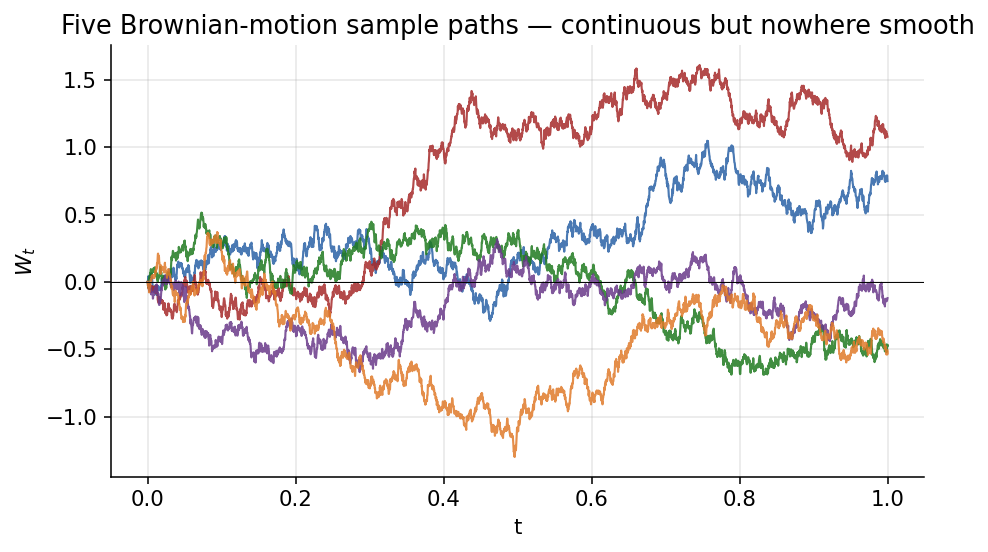
\includegraphics[keepaspectratio]{figures/ch03-bm-paths.png}}
\emph{Five independent sample paths of \(W\) on \([0, 1]\). Every path
is continuous but visibly non-smooth at every scale --- zooming in
reveals identical-looking wiggles. The unbounded-slope property
(3.\(\infty\)) is visible as the path's inability to be ``traced with a
pencil''.}

\[
\frac{\Delta W}{\Delta t} \;\sim\; \frac{\sqrt{\Delta t}}{\Delta t} \;=\; \frac{1}{\sqrt{\Delta t}} \;\longrightarrow\; \infty \quad(\Delta t \downarrow 0).
\]

Every secant slope blows up: the path has no derivative anywhere despite
being everywhere continuous. In any Taylor expansion of \(f(W_t)\), the
second-order term carries \((\Delta W)^2 \sim \Delta t\) --- same order
as \(\Delta t\) itself, never droppable as ``small.''

Coastline analogy: measure with a finer ruler and the \emph{length}
(total variation) grows without bound, while the sum of \emph{squared}
segments (quadratic variation) stays finite and equals \(t\). §3.3
computes the first; §3.4 the second.

Trader gloss. Infinite TV is why no rehedging schedule eliminates
residual cash flows; finite QV \(= t\) is how much residual on average
--- the gamma-theta of options pricing.

\begin{center}\rule{0.5\linewidth}{0.5pt}\end{center}

\section{3.3 Total Variation}\label{total-variation}

\subsection{3.3.1 Definition}\label{definition}

For a function \(f\) on \([0,t]\) and a partition
\(\pi = \{t_0, t_1, \dots, t_N\}\) with
\(0 = t_0 < t_1 < \cdots < t_N = t\), the total variation is

\[
\mathrm{TV}_t \;=\; \lim_{\|\pi\|\downarrow 0}\;\sum_{k} \bigl|\,f(t_k) - f(t_{k-1})\,\bigr|,
\tag{3.9}
\]

where \(\|\pi\| = \max_k (t_k - t_{k-1})\) is the mesh size.
Pictorially, lay the graph of \(f\) flat by flipping each down-stroke
upward; the total horizontal length is \(\mathrm{TV}_t\).

TV matters because the Riemann-Stieltjes integral
\(\int g\,\mathrm{d}f\) only exists (in the classical sense) when \(f\)
has finite total variation on \([0,t]\). For BM we are about to find TV
is infinite, which is exactly why the new stochastic integral of §3.5 is
needed.

\subsection{\texorpdfstring{3.3.2 Case 1 --- \(f\) is differentiable
(finite
TV)}{3.3.2 Case 1 --- f is differentiable (finite TV)}}\label{case-1-f-is-differentiable-finite-tv}

If \(f \in C^1\), by the mean-value theorem there exists
\(t_k^\star \in (t_{k-1}, t_k)\) with
\(\Delta f_k = f'(t_k^\star)\,\Delta t_k\). Therefore

\[
\sum_k |\Delta f_k| \;=\; \sum_k |f'(t_k^\star)|\,\Delta t_k \;\xrightarrow[\|\pi\|\downarrow 0]{}\; \int_0^t |f'(s)|\,\mathrm{d}s \;<\; +\infty.
\tag{3.10}
\]

Finite TV, as expected for smooth functions. The entire argument fails
for BM because \(W\) has no derivative anywhere, and in its absence the
sum of \(|\Delta W_k|\) diverges.

\subsection{3.3.3 Case 2 --- Brownian motion has infinite
TV}\label{case-2-brownian-motion-has-infinite-tv}

For BM the increments are
\(\Delta W_k \stackrel{d}{=} \sqrt{\Delta t_k}\,Z_k\) with
\(Z_k \stackrel{\mathrm{iid}}{\sim} \mathcal{N}(0,1)\). So

\[
\sum_k |W_{t_k} - W_{t_{k-1}}| \;=\; \sum_k \sqrt{\Delta t_k}\,|Z_k|.
\tag{3.11}
\]

The mean. Because \(\mathbb{E}|Z| = \sqrt{2/\pi}\) is a finite constant,

\[
\mathbb{E}\!\left[\sum_k \sqrt{\Delta t_k}\,|Z_k|\right] \;=\; \mathbb{E}|Z|\cdot\sum_k \sqrt{\Delta t_k}.
\tag{3.12}
\]

The variance is \(c^2\sum_k \Delta t_k = c^2 t\), bounded as the
partition refines. The key bound is on the mean:

\[
\sum_k \sqrt{\Delta t_k} \;\ge\; \sum_k \frac{\Delta t_k}{\sqrt{\|\pi\|}} \;=\; \frac{t}{\sqrt{\|\pi\|}} \;\xrightarrow[\|\pi\|\downarrow 0]{}\; +\infty.
\tag{3.13}
\]

So the mean of the TV-sum diverges while its variance stays bounded ---
concentration around an unbounded mean forces the sum itself to be
unbounded. Almost surely,

\[
\boxed{\;\mathrm{TV}_t(W) \;=\; \lim_{\|\pi\|\downarrow 0} \sum_k |W_{t_k} - W_{t_{k-1}}| \;=\; +\infty\;}. \qquad\text{(a.s.)}
\tag{3.14}
\]

BM is too rough for a Riemann-Stieltjes integral
\(\int g\,\mathrm{d}W_s\); a new stochastic integral is needed in §3.5.

Trader gloss. Delta-hedging cost is \(c \sum |\Delta S|\) --- the TV sum
for \(S\). GBM has infinite TV, so frictionless continuous rebalancing
has unbounded cost. The frictionless Black--Scholes derivation is
literally implementable only if transactions are free; in practice
hedgers accept a discrete rebalancing grid and residual gamma risk.

\begin{center}\rule{0.5\linewidth}{0.5pt}\end{center}

\section{\texorpdfstring{3.4 Quadratic Variation and the Rule
\((\mathrm{d}W)^2 = \mathrm{d}t\)}{3.4 Quadratic Variation and the Rule (\textbackslash mathrm\{d\}W)\^{}2 = \textbackslash mathrm\{d\}t}}\label{quadratic-variation-and-the-rule-mathrmdw2-mathrmdt}

\subsection{3.4.1 Definition}\label{definition-1}

The quadratic variation of \(f\) on \([0,t]\) is

\[
[f]_t \;=\; [f,f]_t \;=\; \lim_{\|\pi\|\downarrow 0} \sum_k \bigl(\Delta f_k\bigr)^2, \qquad \Delta f_k = f(t_k) - f(t_{k-1}).
\tag{3.15}
\]

QV measures cumulative \emph{squared jitter}. For smooth \(f\),
\((\Delta f)^2 \sim (\Delta t)^2\) and QV vanishes; for BM,
\((\Delta W)^2 \sim \Delta t\) and the sum stays at \(t\). TV sees
\emph{size}, QV sees \emph{energy} --- BM has finite energy (\(t\)) but
infinite size (\(+\infty\)). Conflating the two is the most common
source of Black--Scholes confusion.

\subsection{\texorpdfstring{3.4.2 Case 1 --- \(f\) differentiable:
\([f]_t = 0\)}{3.4.2 Case 1 --- f differentiable: {[}f{]}\_t = 0}}\label{case-1-f-differentiable-f_t-0}

If \(f \in C^1\),

\[
\sum_k (\Delta f_k)^2 \;=\; \sum_k \bigl(f'(t_k^\star)\bigr)^2\,(\Delta t_k)^2 \;\le\; \|\pi\|\cdot\int_0^t (f'(s))^2\,\mathrm{d}s \;\xrightarrow[\|\pi\|\downarrow 0]{}\; 0.
\tag{3.16}
\]

Smooth functions have zero QV: \((\Delta t_k)^2 \le \|\pi\| \Delta t_k\)
peels off one power of \(\|\pi\|\), killing the sum. BM has
\((\Delta W_k)^2 \sim \Delta t_k\) and the sum stays \(O(1)\) --- the
order retained by the squaring is what produces the Itô correction.

\subsection{\texorpdfstring{3.4.3 Case 2 --- Brownian motion:
\([W,W]_t = t\)}{3.4.3 Case 2 --- Brownian motion: {[}W,W{]}\_t = t}}\label{case-2-brownian-motion-ww_t-t}

Let \(Q = \sum_k (\Delta W_k)^2\) with
\(\Delta W_k \stackrel{d}{=} \sqrt{\Delta t_k}\,Z_k\),
\(Z_k \stackrel{\mathrm{iid}}{\sim}\mathcal{N}(0,1)\).

Mean.

\[
\mathbb{E}[Q] \;=\; \sum_k \mathbb{E}\!\left[(\Delta W_k)^2\right] \;=\; \sum_k \Delta t_k \;=\; t.
\tag{3.17}
\]

The mean is \emph{exact} --- no limit needed, no \(\|\pi\|\) dependence.
Every finite partition already gives \(\mathbb{E}[Q] = t\).

Variance. Using
\(\mathrm{Var}((\Delta W_k)^2) = (\Delta t_k)^2\,\mathrm{Var}(Z^2) = 2(\Delta t_k)^2\)
(because \(\mathrm{Var}(Z^2) = \mathbb{E}[Z^4] - 1 = 3 - 1 = 2\) --- the
standard-Normal fourth moment \(\mathbb{E}[Z^4] = 3\) is derived via the
MGF in §3.7.1) and independence across \(k\),

\[
\mathrm{Var}[Q] \;=\; 2\sum_k (\Delta t_k)^2 \;\le\; 2\,\|\pi\|\sum_k \Delta t_k \;=\; 2\|\pi\|\,t \;\xrightarrow[\|\pi\|\downarrow 0]{}\; 0.
\tag{3.18}
\]

Conclusion. \(Q\) has mean \emph{exactly} \(t\) and variance shrinking
to zero, so by Chebyshev's inequality (\(L^2\)-convergence along the
full sequence, almost-sure along a thinning subsequence):

\[
\boxed{\;\sum_k (\Delta W_k)^2 \;\xrightarrow[\|\pi\|\downarrow 0]{\mathrm{a.s.}}\; t, \qquad [W,W]_t \;=\; t\;} \qquad\text{(a.s.)}
\tag{3.19}
\]

A \emph{random} object --- the sum of squared increments --- converges
to a \emph{deterministic} limit. The convergence is the LLN in Brownian
clothing: \((\Delta W_k)^2 = \Delta t \cdot Z_k^2\) with \(Z_k^2\)
chi-squared-one, and \(\sum Z_k^2/N \to 1\) a.s. This is why implied vol
is observable: QV of log-price is essentially deterministic.

\pandocbounded{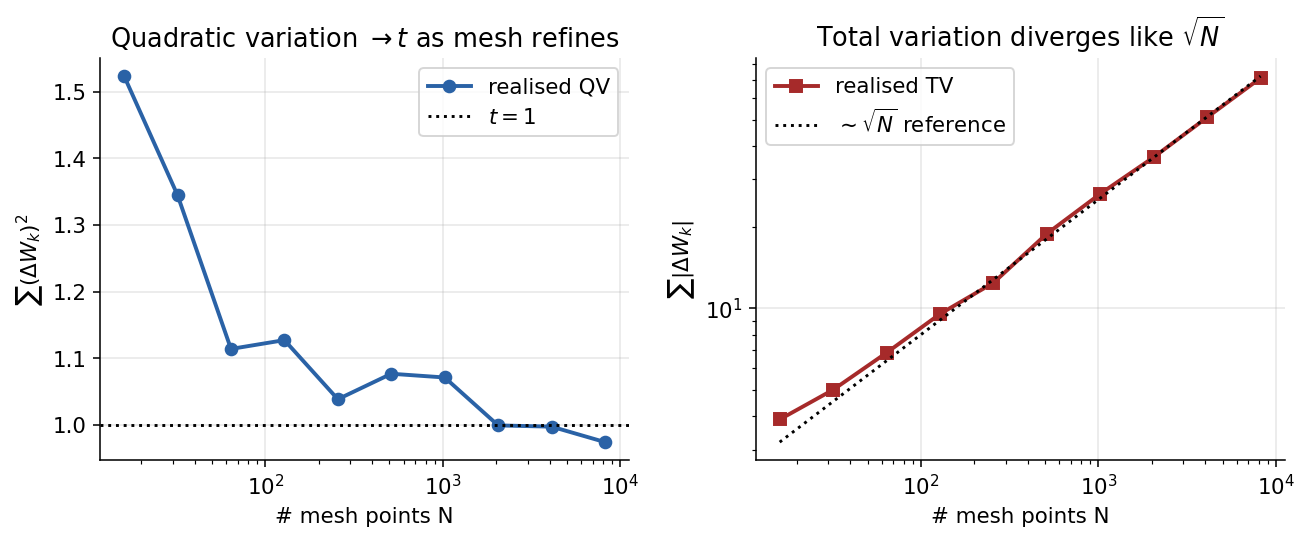
\includegraphics[keepaspectratio]{figures/ch03-qv-convergence.png}}
\emph{The same Brownian path, sampled at progressively finer meshes.
Left: \(\sum(\Delta W_k)^2\) converges deterministically to \(t = 1\) as
the mesh refines. Right: \(\sum|\Delta W_k|\) diverges like \(\sqrt{N}\)
--- finite energy but unbounded path-length.}

\textbf{Variance swaps.} A variance swap pays
\(\frac{252}{N}\sum r_k^2\) on daily log-returns. In GBM
\(r_k \approx \sigma \Delta W_k - \tfrac12\sigma^2 \Delta t\), so
\(\sum r_k^2 \to \sigma^2 t\) --- a deterministic quantity, exactly
replicable by a Carr--Madan log-contract. The TV analogue
(\(\sum |r_k|\)) diverges like \(\sqrt{N}\), which is why ``average
absolute return'' is a nuisance statistic and realised variance is a
well-posed estimator of \(\sigma^2\).

\subsection{\texorpdfstring{3.4.4 The Itô shorthand
\((\mathrm{d}W)^2 = \mathrm{d}t\)}{3.4.4 The Itô shorthand (\textbackslash mathrm\{d\}W)\^{}2 = \textbackslash mathrm\{d\}t}}\label{the-ituxf4-shorthand-mathrmdw2-mathrmdt}

Equation (3.19) justifies the Itô multiplication rules

\[
(\mathrm{d}W_t)^2 \;=\; \mathrm{d}t,\qquad \mathrm{d}W_t\cdot \mathrm{d}t \;=\; 0,\qquad (\mathrm{d}t)^2 \;=\; 0.
\tag{3.20}
\]

Memorisation trick. \(\mathrm{d}W\) lives at scale
\(\sqrt{\mathrm{d}t}\), \(\mathrm{d}t\) at scale \(\mathrm{d}t\). A
product of \(n\) atoms scales as \((\mathrm{d}t)^{n/2}\); keep
\(n = 2\), drop \(n > 2\). Squaring an SDE
\(\mathrm{d}X = a\,\mathrm{d}t + b\,\mathrm{d}W\) collapses to
\(b^2\,\mathrm{d}t\) --- used in every Itô application below. Every
\(\tfrac12\sigma^2\partial_{xx}\) in a pricing PDE traces back to
(3.20).

\begin{figure}
\centering
\pandocbounded{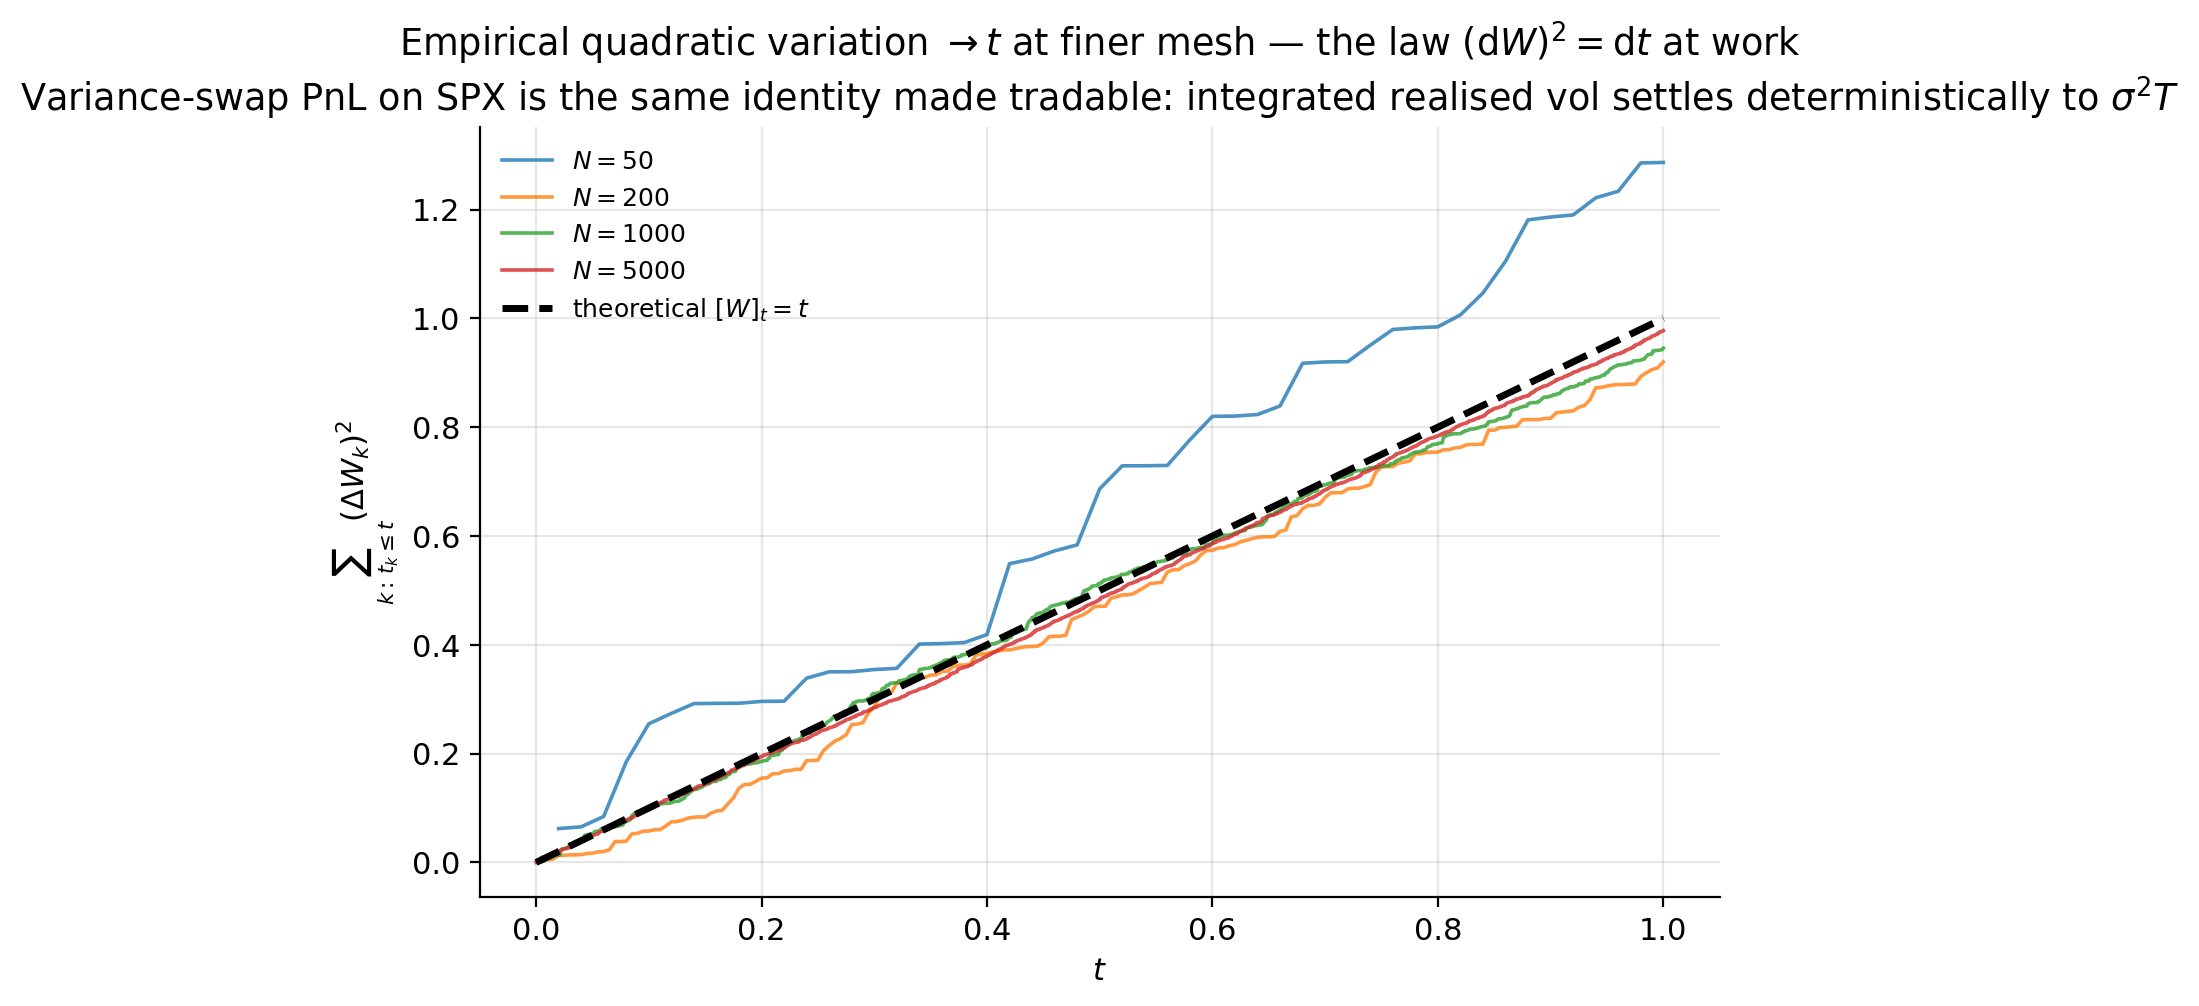
\includegraphics[keepaspectratio]{figures/ch03-ito-multiplication.png}}
\caption{Cumulative sum of squared Brownian increments
\(\sum(\Delta W_k)^2\) as the mesh refines: each path converges to the
deterministic line \([W]_t = t\). The same identity is what makes the
SPX variance swap a \emph{deterministic} payoff in continuous monitoring
--- the realised-variance leg integrates to \(\sigma^2 T\) exactly}
\end{figure}

\subsection{Case study: The ``rule of 16'' --- Brownian scaling in
market
data}\label{case-study-the-rule-of-16-brownian-scaling-in-market-data}

\emph{Every options trader on a US equity desk converts annualised vol
to daily vol by dividing by 16. VIX = 16 means ``expect \(\sim\) 1\%
S\&P moves.'' VIX = 32 means ``expect \(\sim\) 2\% moves.'' This is not
a heuristic --- it is the QV identity (3.19) evaluated at \(t = 1/252\),
and it is one of the few places in finance where a continuous-time
identity is }directly falsifiable* against tick data on any given day.*

\textbf{Context.} The CBOE Volatility Index (VIX) is a model-free 30-day
implied vol on the S\&P 500, quoted in \emph{annualised} units. On 14
May 2026 the VIX closed near 14; through 2024--2025 it traded in a
12--22 range outside of brief stress spikes (March 2020 COVID, August
2024 yen-carry unwind, April 2025 tariff shock). The trading floor's
\emph{rule of 16} --- divide the VIX by 16 to get the implied 1-day
standard deviation in percent --- comes from
\(\sqrt{252} \approx 15.87\). So a VIX of 16 implies a 1-day SPX move of
roughly \(\pm 1\%\); a VIX of 32 implies \(\pm 2\%\); a VIX of 80 (March
2020) implied \(\pm 5\%\). Empirically: in 2024 the VIX averaged
\(\sim\) 15.7, predicting \(\sim\) 0.98\% daily moves, and the realised
one-standard-deviation S\&P 500 daily move that year was 0.84\% ---
within the same order of magnitude, with the small undershoot tracing to
the well-known variance risk premium (implied vol structurally exceeds
realised vol; see Ch 10--11).

\textbf{Math mapping.} This is (3.19) made tradable. Model the S\&P
log-price as Brownian under the risk-neutral measure with annualised
volatility \(\sigma\):
\(\mathrm dS_t/S_t = r\,\mathrm dt + \sigma\,\mathrm dW_t\), so
\(\mathrm d\log S_t = (r - \tfrac12\sigma^2)\,\mathrm dt + \sigma\,\mathrm dW_t\).
The QV identity (3.19) gives \([\log S, \log S]_t = \sigma^2 t\).
Equivalently, the variance of the log-return over horizon \(\Delta t\)
is \(\sigma^2 \Delta t\) and the standard deviation is
\(\sigma\sqrt{\Delta t}\). With \(\Delta t = 1/252\) trading days and
\$\sigma = \$ VIX\(/100\), this gives
\(\text{StDev}_{\text{daily}} = \text{VIX}/(100 \cdot \sqrt{252}) \approx \text{VIX}/1587\),
and quoting the result in percent removes the factor of 100:
\(\text{StDev}_{\text{daily}}(\%) \approx \text{VIX}/\sqrt{252} \approx \text{VIX}/16\).
The \(\sqrt{t}\) scaling is \emph{not} a model assumption --- it is
forced by the QV identity, which holds for any continuous semimartingale
with absolutely continuous QV. So when the rule-of-16 prediction matches
realised daily standard deviations, you are confirming that the path is
locally Brownian; when it fails, the path has acquired roughness
inconsistent with \([W, W]_t = t\).

\textbf{Lesson.} Three failure modes a desk watches for. First,
\emph{gap moves at the open}: 17 Sept 2008 (Lehman week, S\&P opened
\(-4.7\%\) on a VIX-implied \(\sim\) 2\% one-day SD) and 16 March 2020
(COVID, S\&P open down \(-7\%\) vs VIX-implied \(\sim\) 5\%) blew
through the daily standard deviation by 2--3\(\sigma\) each --- the path
is not continuous overnight, and overnight returns satisfy a different
scaling regime than intraday returns (the QV of an overnight gap is
\emph{concentrated}, not spread out at \(\sqrt t\)). Second,
\emph{vol-of-vol regimes}: in stress episodes the VIX itself moves
20--30\% intraday, so the rule-of-16 conversion using yesterday's VIX
systematically under-predicts today's moves; this is the phenomenon
Heston-style stochastic vol models (Ch 10) are built to capture. Third,
\emph{jump components}: equity microstructure has a jump component
(earnings, central bank meetings, exchange-pause incidents) that
contributes additional QV beyond the diffusive
\(\sigma^2 \,\mathrm dt\); the rule-of-16 implicitly assumes pure
diffusion. Operationally, a desk computes a ``realised-vs-implied
ratio'' daily --- realised standard deviation of one-minute returns
scaled to daily, divided by VIX/16 --- and uses sustained excursions
above 1.0 as a signal that the diffusive Brownian model is locally
inadequate and one should trade vol-of-vol products (VVIX,
variance-of-variance swaps) instead of plain vol.

\begin{center}\rule{0.5\linewidth}{0.5pt}\end{center}

\section{3.5 The Itô Stochastic
Integral}\label{the-ituxf4-stochastic-integral}

\subsection{3.5.1 Warm-up --- the classical Riemann-Stieltjes
integral}\label{warm-up-the-classical-riemann-stieltjes-integral}

For smooth \(f\) the chain rule gives

\[
\int_0^t f(s)\,\mathrm{d}f(s) \;=\; \tfrac{1}{2}\,\bigl(f^2(t) - f^2(0)\bigr),
\tag{3.21}
\]

because
\(\mathrm{d}\bigl(\tfrac{1}{2}f^2(s)\bigr) = f(s)\,\mathrm{d}f(s)\).
Remember this answer --- when we repeat the calculation for Brownian
motion we will find the analogue carries an \emph{extra} \(-\tfrac12 t\)
term that has no classical counterpart. The classical integral is
oblivious to the endpoint choice in the Riemann sum because QV is zero;
once we swap \(f\) for BM the endpoint choice becomes consequential, and
the \(-\tfrac12 t\) is exactly the accumulated left-right mismatch
summed over infinitely many infinitesimal intervals.

\subsection{3.5.2 The Itô integral,
defined}\label{the-ituxf4-integral-defined}

The stochastic analogue uses \emph{left-endpoint} Riemann sums ---
crucial, because this is what makes the integral a martingale:

\[
\int_0^t W_s\,\mathrm{d}W_s \;\equiv\; \lim_{\|\pi\|\downarrow 0}\;\sum_k W_{t_{k-1}}\,\Delta W_{t_k}, \qquad \Delta W_{t_k} = W_{t_k} - W_{t_{k-1}}.
\tag{3.22}
\]

Left-endpoint evaluation makes \(W_{t_{k-1}}\) independent of
\(\Delta W_{t_k}\), so each summand has zero expectation and the
integral is a martingale. The Itô integral encodes a \emph{predictable}
strategy: position size committed before the move, not after.
Right-endpoint or midpoint (Stratonovich) rules obey the classical chain
rule but break the martingale property --- fatal in finance, where
no-arbitrage demands ``predictable strategies earn zero expected P\&L.''

\subsection{\texorpdfstring{3.5.3 First worked integral ---
\(\int_0^t W_s\,\mathrm{d}W_s\)}{3.5.3 First worked integral --- \textbackslash int\_0\^{}t W\_s\textbackslash,\textbackslash mathrm\{d\}W\_s}}\label{first-worked-integral-int_0t-w_smathrmdw_s}

The claim, which we prove by a telescoping identity + QV computation, is

\[
I_t \;=\; \int_0^t W_s\,\mathrm{d}W_s \;=\; \tfrac12\,W_t^2 \;-\; \tfrac12\,t \qquad\text{a.s.}
\tag{3.23}
\]

The answer already carries the surprise: the classical guess would be
\(\tfrac12 W_t^2\), but the stochastic integral subtracts an extra
\(\tfrac12 t\) --- the \emph{Itô correction}, sometimes called the
``convexity correction'' because it arises from the curvature of
\(w \mapsto \tfrac12 w^2\) interacting with the QV of \(W\). The
\(\tfrac12 t\) is deterministic, grows linearly, and has no stochastic
component; it is the ``free'' cash that a convex long-gamma position
accumulates as time passes. In options language, the correction is the
\emph{theta bleed} of a one-lot long-gamma portfolio.

\textbf{Proof.} Use the algebraic identity
\(a(b-a) = \tfrac12(b^2 - a^2) - \tfrac12(b-a)^2\) with
\(a = W_{t_{k-1}}\), \(b = W_{t_k}\):

\[
W_{t_{k-1}}\bigl(W_{t_k} - W_{t_{k-1}}\bigr) \;=\; \tfrac{1}{2}\bigl(W_{t_k}^2 - W_{t_{k-1}}^2\bigr) \;-\; \tfrac{1}{2}\bigl(W_{t_k} - W_{t_{k-1}}\bigr)^2.
\tag{3.24}
\]

Summing over \(k\) and using \(W_0 = 0\):

\[
\sum_k W_{t_{k-1}}\,\Delta W_{t_k} \;=\; \tfrac{1}{2}\,W_t^2 \;-\; \tfrac{1}{2}\,\sum_k (\Delta W_{t_k})^2.
\tag{3.25}
\]

The left-hand side is the Riemann-like sum defining the Itô integral.
The right-hand side has two parts. The first, \(\tfrac12 W_t^2\), is the
classical Newton-Leibniz answer. The second,
\(-\tfrac12 \sum_k(\Delta W_{t_k})^2\), is the Itô correction in
discrete form --- an exact lattice version of \(-\tfrac12 t\), because
by (3.19) this sum converges almost surely to \(t\). Passing to the
limit,

\[
\boxed{\;\int_0^t W_s\,\mathrm{d}W_s \;=\; \tfrac{1}{2}\,W_t^2 \;-\; \tfrac{1}{2}\,t\;}.
\tag{3.26}
\]

Three observations on this answer.

\begin{enumerate}
\def\labelenumi{\arabic{enumi}.}
\tightlist
\item
  Taking expectations on both sides of (3.26):
  \(\mathbb{E}\int_0^t W_s\,\mathrm{d}W_s = \tfrac12\mathbb{E}[W_t^2] - \tfrac12 t = 0\).
  The Itô integral is zero-mean --- the martingale property surfaces
  automatically.
\item
  The Itô integral is \emph{not} zero, despite having zero mean. Its
  variance grows with \(t\) (we'll compute it via the Itô isometry
  next): it is a non-trivial random variable concentrated around zero.
\item
  The difference \(I_t - \tfrac12 W_t^2 = -\tfrac12 t\) is
  \emph{deterministic}. Remarkable: the randomness of the classical
  antiderivative \(\tfrac12 W_t^2\) and the randomness of the Itô
  integral \(I_t\) match exactly, so when subtracted they leave only the
  \(-\tfrac12 t\) correction.
\end{enumerate}

Equivalent form: rearranging (3.26),

\[
\tfrac{1}{2}\,W_t^2 \;=\; \int_0^t W_s\,\mathrm{d}W_s \;+\; \tfrac{1}{2}\,t,
\tag{3.27}
\]

which is Itô's formula applied to \(F(w) = \tfrac12 w^2\):
\(\mathrm{d}(\tfrac12 W_t^2) = W_t\,\mathrm{d}W_t + \tfrac12\,\mathrm{d}t\).
The \(\tfrac12\,\mathrm{d}t\) correction is exactly what distinguishes
the stochastic integral from the classical chain-rule answer.

\subsection{3.5.4 Why the left-endpoint choice
matters}\label{why-the-left-endpoint-choice-matters}

A right-endpoint \(W_{t_k}\) would flip the sign of the QV correction in
the telescoping identity, giving \(+\tfrac12 t\) and the classical
answer \(\tfrac12 W_t^2\). Worse, it would couple the integrand to its
driving noise --- anticipative, hence inadmissible in continuous-time
finance. The left-endpoint rule is the mathematical enforcement of
no-arbitrage.

\begin{center}\rule{0.5\linewidth}{0.5pt}\end{center}

\section{3.6 The Itô Isometry}\label{the-ituxf4-isometry}

The \(L^2\)-isometry reduces any variance-of-stochastic-integral
calculation to an ordinary time integral, and structurally asserts the
Itô integral is a continuous linear map from \(L^2\) integrands into
martingales.

\textbf{Statement.} For any two adapted integrands \(g_s\) and \(h_s\)
satisfying \(\mathbb{E}\int_0^t g_s^2\,\mathrm{d}s < \infty\) and
likewise for \(h\),

\[
\boxed{\;\mathbb{E}\!\left[\,\Big(\int_0^t g_s\,\mathrm{d}W_s\Big)\Big(\int_0^t h_s\,\mathrm{d}W_s\Big)\,\right]
\;=\; \mathbb{E}\!\left[\,\int_0^t g_s h_s\,\mathrm{d}s\,\right]\;}.
\tag{3.28}
\]

In particular, for \(g = h\), the \(L^2\)-norm of a stochastic integral
equals the \(L^2\)-norm (in \(s\) and \(\omega\)) of its integrand:

\[
\mathbb{E}\!\left[\left(\int_0^t g_s\,\mathrm{d}W_s\right)^{\!2}\right] \;=\; \mathbb{E}\!\int_0^t g_s^2\,\mathrm{d}s.
\tag{3.29}
\]

\textbf{Proof --- the A + B + C decomposition.} Set \(g_t = g(t, W_t)\),
\(h_t = h(t, W_t)\), and define the residual

\[
\mathcal{E} \;=\; \mathbb{E}\!\left[\Big(\int_0^t g_s\,\mathrm{d}W_s\Big)\Big(\int_0^t h_s\,\mathrm{d}W_s\Big) \;-\; \int_0^t g_s h_s\,\mathrm{d}s\right].
\tag{3.30}
\]

Goal: show \(\mathcal{E} = 0\). Fix a partition
\(\pi = \{0 = t_0 < t_1 < \cdots < t_n = t\}\) and discretise both
integrals as Riemann sums, so the first product becomes

\[
\Big(\sum_k g_{t_{k-1}}\Delta W_{t_k}\Big)\Big(\sum_j h_{t_{j-1}}\Delta W_{t_j}\Big)
\;=\; \sum_{k,j} g_{k-1}\,h_{j-1}\,\Delta W_{t_k}\,\Delta W_{t_j},
\]

where \(g_{k-1} = g_{t_{k-1}}\) etc. The second piece (the time
integral) discretises as \(\sum_k g_{k-1}\,h_{k-1}\,\Delta t_k\).

\textbf{Step 1 --- Split the double sum into three regions} (A, B, C)
according to the relationship between indices \(j\) and \(k\):

\[
\sum_{k,j} g_{k-1}\,h_{j-1}\,\Delta W_{k}\,\Delta W_{j}
\;=\; \underbrace{\sum_{k<j} g_{k-1}\,h_{j-1}\,\Delta W_k\,\Delta W_j}_{A} \;+\; \underbrace{\sum_{j<k} g_{k-1}\,h_{j-1}\,\Delta W_k\,\Delta W_j}_{B} \;+\; \underbrace{\sum_k g_{k-1}\,h_{k-1}\,(\Delta W_k)^2}_{C}.
\]

\begin{figure}
\centering
\pandocbounded{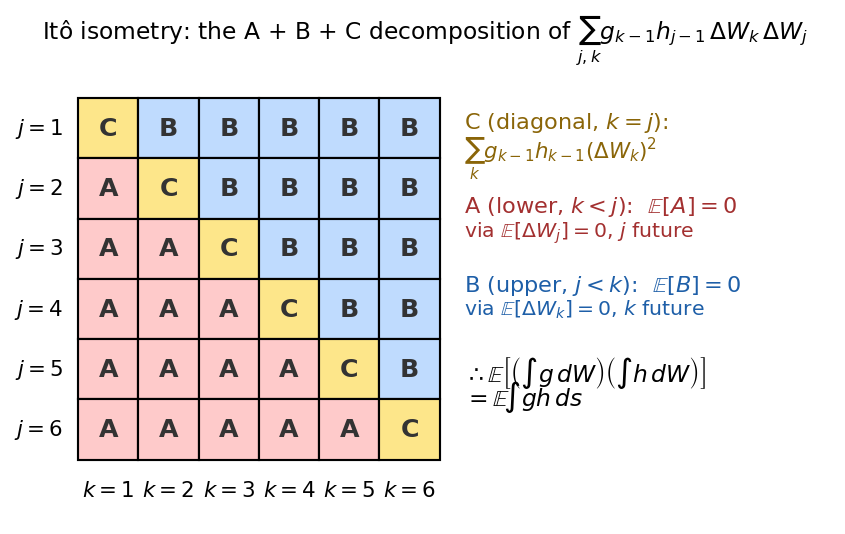
\includegraphics[keepaspectratio]{figures/ch03-ito-isometry-proof.png}}
\caption{Itô isometry proof: A + B + C matrix decomposition}
\end{figure}

The matrix picture: the \(n\times n\) grid indexed by \((k,j)\) splits
into the lower triangle \(A\) (\(k<j\)), the upper triangle \(B\)
(\(j<k\)), and the diagonal \(C\) (\(k=j\), highlighted). The isometry
is the claim that the two triangles die in expectation and only the
diagonal survives --- matching the time-integral piece exactly.

\textbf{Step 2 --- \(\mathbb{E}[A] = 0\).} For any term in \(A\) we have
\(k < j\). Condition on \(\mathcal{F}_{t_{j-1}}\): the factors
\(g_{k-1}\), \(h_{j-1}\), and \(\Delta W_k\) are all
\(\mathcal{F}_{t_{j-1}}\)-measurable (by convention
\(h_{j-1} := h_{t_{j-1}}\) is \(\mathcal{F}_{t_{j-1}}\)-measurable
because it is evaluated at the left endpoint of the \(j\)-th
sub-interval; \(g_{k-1}\) and \(\Delta W_k\) are
\(\mathcal{F}_{t_k}\subset\mathcal{F}_{t_{j-1}}\)-measurable since
\(k < j \Rightarrow t_k \le t_{j-1}\)), while \(\Delta W_j\) is
independent of \(\mathcal{F}_{t_{j-1}}\) with mean zero. Hence

\[
\mathbb{E}\!\left[g_{k-1}\,h_{j-1}\,\Delta W_k\,\Delta W_j\right]
\;=\; \mathbb{E}\!\left[g_{k-1}\,h_{j-1}\,\Delta W_k\right]\cdot\underbrace{\mathbb{E}[\Delta W_j]}_{=\,0}
\;=\; 0,
\tag{3.31}
\]

and summing over \(k<j\) gives \(\mathbb{E}[A] = 0\).

\textbf{Step 3 --- \(\mathbb{E}[B] = 0\)} by the symmetric argument with
the roles of \(j\) and \(k\) swapped.

\textbf{Step 4 --- Only the diagonal \(C\) survives.} Combining the
three pieces with the time-integral subtraction,

\[
\mathcal{E} \;=\; \mathbb{E}\!\left[\sum_k g_{k-1}\,h_{k-1}\,\bigl((\Delta W_k)^2 - \Delta t_k\bigr)\right]
\;=\; \sum_k \mathbb{E}[g_{k-1}\,h_{k-1}]\cdot\underbrace{\mathbb{E}[(\Delta W_k)^2 - \Delta t_k]}_{=\,0}
\;=\; 0,
\tag{3.32}
\]

using independence of \(g_{k-1} h_{k-1}\) (measurable at \(t_{k-1}\))
from \(\Delta W_k\), and \(\mathbb{E}[(\Delta W_k)^2] = \Delta t_k\).

\textbf{Step 5 --- Pass to the limit.} Equation (3.32) holds for every
partition \(\pi\); taking \(\|\pi\|\downarrow 0\) delivers the isometry
(3.28). \(\blacksquare\)

\textbf{Reading the isometry.} The scalar identity \([W,W]_t = t\)
becomes, under weighting by \(g_s^2\), the statement that the variance
of \(\int g\,\mathrm{d}W\) equals the integrated squared integrand. In a
quant-practitioner translation: ``the variance of a stochastic P\&L
equals the integrated variance contribution of each sub-interval's
position.'' Every variance-swap argument in the rest of the guide is
downstream of (3.29).

A weakening of the boundedness assumption gives the result for any \(g\)
with \(\mathbb{E}\int_0^t g_s^2\,\mathrm{d}s < \infty\), via a standard
localisation-and-approximation argument. We take this extension for
granted from here on.

\begin{center}\rule{0.5\linewidth}{0.5pt}\end{center}

\section{3.7 Brownian Moment
Calculations}\label{brownian-moment-calculations}

A small toolkit of moment calculations, each a one-liner via the
Gaussian MGF \(h(a) = e^{a^2/2}\) (\(\mathbb{E}[Z^n] = h^{(n)}(0)\)) or
the increment decomposition \(W_t = W_s + (W_t - W_s)\) with the second
piece independent of the first.

\subsection{\texorpdfstring{3.7.1 Variance of
\(W_t^2\)}{3.7.1 Variance of W\_t\^{}2}}\label{variance-of-w_t2}

Starting from
\(\mathrm{Var}[W_t^2] = \mathbb{E}[W_t^4] - (\mathbb{E}[W_t^2])^2\) and
using \(W_t \stackrel{d}{=} \sqrt{t}\,Z\) with
\(Z\sim\mathcal{N}(0,1)\),

\[
\mathrm{Var}[W_t^2] \;=\; t^2\,\bigl(\mathbb{E}[Z^4] - 1\bigr).
\tag{3.33}
\]

The Gaussian MGF \(h(a) = e^{a^2/2}\) has derivatives
\(h'(a) = a e^{a^2/2}\), \(h''(a) = (1+a^2)e^{a^2/2}\),
\(h'''(a) = (a^3 + 3a)e^{a^2/2}\),
\(h^{(4)}(a) = (a^4 + 6a^2 + 3)e^{a^2/2}\). Evaluating at \(a=0\):
\(\mathbb{E}[Z^2] = 1\), \(\mathbb{E}[Z^4] = 3\). The odd moments vanish
by symmetry; the even moments grow as
\((2k-1)!! = 1, 3, 15, 105,\dots\). Substituting,

\[
\boxed{\;\mathrm{Var}[W_t^2] \;=\; 2\,t^2\;}.
\tag{3.34}
\]

This is the Brownian analogue of \(\mathrm{Var}(X^2) = 2\sigma^4\) for
centred Gaussians with variance \(\sigma^2 = t\), and it underlies the
QV concentration argument of §3.4 (the variance of the QV sum is
\(\sum 2(\Delta t_k)^2 \le 2\|\pi\|\,t\)).

\subsection{\texorpdfstring{3.7.2 Covariance
\(\mathbb{E}[W_t W_s]\)}{3.7.2 Covariance \textbackslash mathbb\{E\}{[}W\_t W\_s{]}}}\label{covariance-mathbbew_t-w_s}

For \(0 \le s \le t\), write \(W_t = (W_t - W_s) + W_s\). Then

\[
\mathbb{E}[W_t\,W_s] \;=\; \mathbb{E}[(W_t - W_s)\,W_s] \;+\; \mathbb{E}[W_s^2] \;=\; 0 \;+\; s,
\]

because \(W_s\) and the forward increment \(W_t - W_s\) are independent
mean-zero. Hence

\[
\boxed{\;\mathbb{E}[W_t\,W_s] \;=\; \min(s,t)\;}.
\tag{3.35}
\]

The correlation is \(\mathrm{Corr}(W_t, W_s) = \sqrt{s/t}\): nearby
times are highly correlated, far-apart times nearly independent. This is
also the kernel used when simulating BM on a grid --- for \(s<t\) the
joint law \((W_s, W_t)\) is Gaussian with covariance matrix
\(\begin{pmatrix}s & s\\ s & t\end{pmatrix}\), whose Cholesky
factorisation gives the practical recipe ``draw \(Z_1, Z_2\) i.i.d.
standard normal; set \(W_s = \sqrt{s}Z_1\),
\(W_t = \sqrt{s}Z_1 + \sqrt{t-s}Z_2\).''

\subsection{3.7.3 The exponential
martingale}\label{the-exponential-martingale}

A recurring character in this guide. Claim:

\[
\boxed{\;\mathbb{E}[X_t] \;=\; 1 \quad\text{for every } t\ge 0\;}, \qquad X_t = e^{-\tfrac12\sigma^2 t + \sigma W_t}.
\tag{3.36}
\]

Proof by MGF:

\[
\mathbb{E}[X_t] \;=\; e^{-\tfrac12\sigma^2 t}\,\mathbb{E}[e^{\sigma W_t}] \;=\; e^{-\tfrac12\sigma^2 t}\,e^{\tfrac12\sigma^2 t} \;=\; 1,
\]

using the Gaussian MGF. The drift \(-\tfrac12\sigma^2 t\) exactly
offsets the Jensen bump
\(\mathbb{E}[e^{\sigma W_t}] = e^{\sigma^2 t/2}\) from exponentiating a
Gaussian. This is the origin of the \(-\tfrac12\sigma^2\) in the GBM
log-drift: a bare \(rt\) drift would let \(S_t/S_0\) grow in expectation
and break the \(\mathbb{Q}\)-martingale property of the discounted
stock.

More generally, for any real exponent \(c\),

\[
\mathbb{E}[X_t^c] \;=\; e^{-\tfrac12 c\sigma^2 t}\cdot e^{\tfrac12 c^2\sigma^2 t} \;=\; e^{\tfrac12 c(c-1)\sigma^2 t}.
\tag{3.37}
\]

For \(c=0\) and \(c=1\) the right-hand side equals \(1\) --- these are
the two ``zero Jensen bump'' cases. For \(c=2\) it gives
\(\mathbb{E}[X_t^2] = e^{\sigma^2 t}\), from which
\(\mathrm{Var}(X_t) = e^{\sigma^2 t} - 1\) --- the well-known log-normal
variance. A stronger statement, proved in §3.9 below, is that \(X_t\)
satisfies the SDE \(\mathrm{d}X_t = \sigma X_t\,\mathrm{d}W_t\) and is
therefore a martingale.

\subsection{3.7.4 Two Itô-integral variances via
isometry}\label{two-ituxf4-integral-variances-via-isometry}

As a quick application of (3.29), let us compute the variance of two Itô
integrals that we will meet repeatedly.

First, \(I_t = \int_0^t W_s\,\mathrm{d}W_s\). By Itô isometry,

\[
\mathrm{Var}[I_t] \;=\; \mathbb{E}\!\left[\int_0^t W_s^2\,\mathrm{d}s\right] \;=\; \int_0^t s\,\mathrm{d}s \;=\; \tfrac12 t^2.
\tag{3.38}
\]

A sanity check comes from the closed-form \(I_t = \tfrac12(W_t^2 - t)\):
then
\(\mathrm{Var}[I_t] = \tfrac14\mathbb{E}[(W_t^2 - t)^2] = \tfrac14(3t^2 - 2t^2 + t^2) = \tfrac12 t^2\).
Both routes agree.

Second, \(J_t = \int_0^t e^{W_s}\,\mathrm{d}W_s\). The integrand is not
Gaussian, so \(J_t\) is not Gaussian either, but its variance still
follows from (3.29):

\[
\mathrm{Var}[J_t] \;=\; \int_0^t \mathbb{E}[e^{2W_s}]\,\mathrm{d}s \;=\; \int_0^t e^{2s}\,\mathrm{d}s \;=\; \tfrac12(e^{2t} - 1),
\tag{3.39}
\]

using \(\mathbb{E}[e^{\alpha W_s}] = e^{\alpha^2 s/2}\). More generally,
when the integrand is \(e^{\alpha W_s}\), the variance of the Itô
integral is \((e^{\alpha^2 t} - 1)/\alpha^2\). This is the template for
every ``expectation of an exponential Brownian function'' in the guide,
and we will reuse it without comment.

\begin{center}\rule{0.5\linewidth}{0.5pt}\end{center}

\section{3.8 Itô's Lemma for Brownian
Motion}\label{ituxf4s-lemma-for-brownian-motion}

Itô's lemma is the chain rule of stochastic calculus and the single most
important tool in this guide. The spirit: Taylor expand one extra term,
keep only first-order in \(\mathrm{d}W\) and second-order in
\(\mathrm{d}W\) (the latter is \(\mathrm{d}t\) by (3.20)).

\subsection{3.8.1 Setup}\label{setup}

Fix a smooth function \(f(t, w)\) with \(f \in C^{1,2}\)
(once-differentiable in \(t\), twice-differentiable in \(w\), with
continuous derivatives), and define the process

\[
X_t \;=\; f(t,\,W_t).
\tag{3.40}
\]

One derivative in \(t\), two in \(w\) --- the second-order \(w\)-term
survives via \((\mathrm{d}W)^2 = \mathrm{d}t\) and contributes
\(\tfrac12\partial_{ww}f\,\mathrm{d}t\). Kink payoffs like \((S - K)_+\)
fail \(C^{1,2}\) and need Tanaka's formula (boundary-delta terms); we
treat them informally.

\subsection{3.8.2 Heuristic derivation via Taylor
expansion}\label{heuristic-derivation-via-taylor-expansion}

Start with the generic Taylor expansion of
\(f(t+\Delta t,\,W_{t+\Delta t})\) around \((t, W_t)\):

\[
\begin{aligned}
f(t+\Delta t,\, W_{t+\Delta t}) \;-\; f(t, W_t)
\;=\; &\partial_t f\,\Delta t \\
+\;&\partial_w f\,\Delta W \\
+\;&\tfrac12\,\partial_{tt} f\,(\Delta t)^2 \\
+\;&\partial_{tw} f\,\Delta t\,\Delta W \\
+\;&\tfrac12\,\partial_{ww} f\,(\Delta W)^2 \\
+\;&\text{higher-order terms},
\end{aligned}
\]

with \(\Delta W = W_{t+\Delta t} - W_t\). Which terms are
\(O(\Delta t)\) (the ``dominant'' scale in the limit)?

{\def\LTcaptype{none} % do not increment counter
\begin{longtable}[]{@{}
  >{\raggedright\arraybackslash}p{(\linewidth - 4\tabcolsep) * \real{0.3333}}
  >{\raggedright\arraybackslash}p{(\linewidth - 4\tabcolsep) * \real{0.3333}}
  >{\raggedright\arraybackslash}p{(\linewidth - 4\tabcolsep) * \real{0.3333}}@{}}
\toprule\noalign{}
\begin{minipage}[b]{\linewidth}\raggedright
Term
\end{minipage} & \begin{minipage}[b]{\linewidth}\raggedright
Magnitude scaling
\end{minipage} & \begin{minipage}[b]{\linewidth}\raggedright
Keep or drop?
\end{minipage} \\
\midrule\noalign{}
\endhead
\bottomrule\noalign{}
\endlastfoot
\(\partial_t f\,\Delta t\) & \(\Delta t\) & Keep (deterministic
drift) \\
\(\partial_w f\,\Delta W\) & \(\sqrt{\Delta t}\) & Keep (stochastic
term) \\
\(\tfrac12 \partial_{ww} f\,(\Delta W)^2\) & \(\Delta t\) & Keep (Itô
correction) \\
\(\tfrac12 \partial_{tt} f\,(\Delta t)^2\) & \((\Delta t)^2\) & Drop \\
\(\partial_{tw} f\,\Delta t\,\Delta W\) & \((\Delta t)^{3/2}\) & Drop \\
higher-order & \(\le (\Delta t)^{3/2}\) & Drop \\
\end{longtable}
}

In ordinary calculus the second-order term would be \(O((\Delta t)^2)\)
and discarded. But for Brownian motion \((\Delta W)^2 \approx \Delta t\)
by (3.20) --- the second-order term is the \emph{same order} as
\(\Delta t\), so it must be kept. Cross terms \(\Delta t\cdot\Delta W\)
and \((\Delta t)^2\) are of strictly higher order and vanish.

Taking the infinitesimal limit yields

\[
\boxed{\;\mathrm{d}X_t \;=\; \left[\partial_t f(t, W_t) \;+\; \tfrac{1}{2}\,\partial_{ww} f(t, W_t)\right]\mathrm{d}t \;+\; \partial_w f(t, W_t)\,\mathrm{d}W_t\;}.
\tag{3.41}
\]

In integrated form:

\[
X_t - X_0 \;=\; \int_0^t \left[\partial_s f + \tfrac{1}{2}\partial_{ww} f\right]\mathrm{d}s \;+\; \int_0^t \partial_w f\,\mathrm{d}W_s.
\tag{3.42}
\]

The first integral is an ordinary Riemann integral; the second is a
stochastic integral of the type defined in (3.22).

\textbf{Reading (3.41).} Drift + martingale: a bounded-variation
Lebesgue piece plus an Itô integral that carries all the QV. This is the
Doob--Meyer decomposition for Itô processes. Taking expectations kills
the martingale and leaves
\(\mathbb{E}[f(t, W_t)] - f(0, 0) = \int_0^t \mathbb{E}[\partial_s f + \tfrac12 \partial_{ww}f]\,\mathrm{d}s\)
--- the engine of the Feynman--Kac derivations in Ch. 4.

\pandocbounded{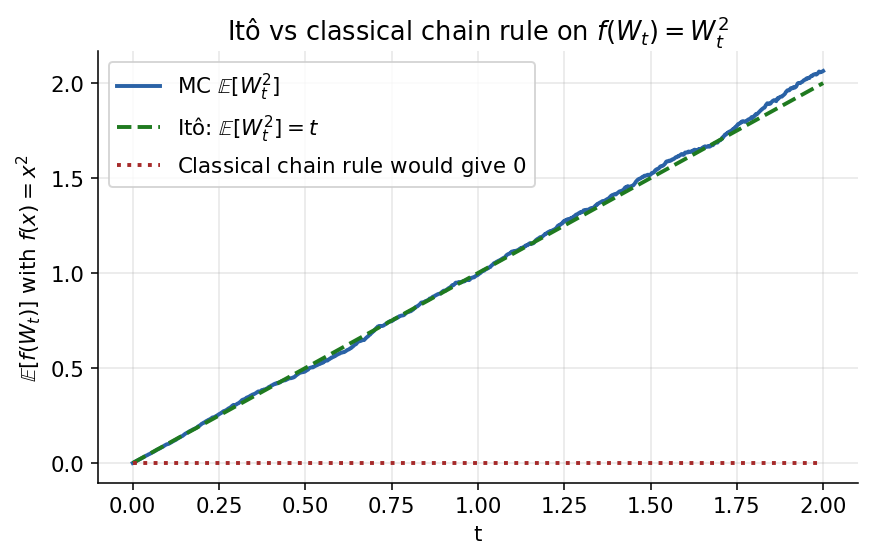
\includegraphics[keepaspectratio]{figures/ch03-ito-vs-chain.png}}
\emph{Monte-Carlo \(\mathbb{E}[W_t^2]\) tracks the Itô prediction \(t\)
(green dashed), not the classical chain rule's \(0\) (red dotted). The
gap is the Itô correction \(\tfrac12 f''\,\mathrm{d}t = \mathrm{d}t\)
integrated from \(0\) to \(t\) --- precisely the drift contribution that
ordinary calculus discards.}

\subsection{3.8.3 Reading the formula --- options-language
translation}\label{reading-the-formula-options-language-translation}

For \(X_t = f(t, W_t)\) interpreted as an option price with \(W_t\)
being the underlying:

\begin{itemize}
\tightlist
\item
  \(\partial_t f\) is \textbf{theta} --- the passage-of-time
  sensitivity.
\item
  \(\partial_w f\) is \textbf{delta} --- the underlying sensitivity.
\item
  \(\partial_{ww} f\) is \textbf{gamma} --- the curvature of price
  versus underlying.
\end{itemize}

Itô then reads: option P\&L = theta\(\cdot\mathrm{d}t\) +
delta\(\cdot\mathrm{d}W\) + \(\tfrac12\)gamma\(\cdot\mathrm{d}t\). The
last term is the gamma-theta trade-off --- long-gamma books bleed theta
and earn gamma P\&L; short-gamma books do the reverse. The \(\tfrac12\)
is just Taylor's second-order coefficient, not a normalisation mystery.

\subsection{3.8.4 Three worked Itô-lemma
examples}\label{three-worked-ituxf4-lemma-examples}

\textbf{Example 1 --- \(\int W\,\mathrm{d}W\) via Itô.}

Goal: compute \(\int_0^t W_s\,\mathrm{d}W_s\) using Itô's lemma rather
than the telescoping identity of §3.5.

Choose \(f(t,w) = \tfrac12 w^2\), so \(\partial_t f = 0\),
\(\partial_w f = w\), \(\partial_{ww}f = 1\). Plugging into (3.41):

\[
\mathrm{d}(\tfrac12 W_t^2) \;=\; \tfrac12\,\mathrm{d}t \;+\; W_t\,\mathrm{d}W_t.
\]

Integrating from \(0\) to \(t\) with \(W_0 = 0\) gives
\(\tfrac12 W_t^2 = \tfrac12 t + \int_0^t W_s\,\mathrm{d}W_s\), so

\[
\int_0^t W_s\,\mathrm{d}W_s \;=\; \tfrac12 W_t^2 - \tfrac12 t,
\tag{3.43}
\]

in agreement with (3.26). Four lines instead of the full telescoping
proof of §3.5 --- Itô's lemma is massively more efficient.

\textbf{Example 2 --- \(\int W^2\,\mathrm{d}W\).}

Choose \(f(t,w) = \tfrac13 w^3\), so \(\partial_t f = 0\),
\(\partial_w f = w^2\), \(\partial_{ww} f = 2w\). Plugging into (3.41):

\[
\mathrm{d}(\tfrac13 W_t^3) \;=\; W_t\,\mathrm{d}t \;+\; W_t^2\,\mathrm{d}W_t.
\]

Integrating and solving for the stochastic integral:

\[
\boxed{\;\int_0^t W_s^2\,\mathrm{d}W_s \;=\; \tfrac13 W_t^3 \;-\; \int_0^t W_s\,\mathrm{d}s\;}.
\tag{3.44}
\]

The remaining \(\int_0^t W_s\,\mathrm{d}s\) is an ordinary pathwise
Riemann integral, not a stochastic one. Itô has converted the stochastic
integral into (algebraic term) \(+\) (pathwise integral). The pathwise
piece cannot be eliminated algebraically --- it depends on the
\emph{entire path} \((W_s)_{s\in[0,t]}\), not just the endpoint \(W_t\).
Its distribution is Gaussian with
\(\mathrm{Var}\!\int_0^t W_s\,\mathrm{d}s = \int_0^t\!\int_0^t \min(u,v)\,\mathrm{d}u\,\mathrm{d}v = \tfrac13 t^3\).

\textbf{Example 3 --- the exponential martingale.}

Goal: given \(X_t = e^{-\tfrac12\sigma^2 t + \sigma W_t}\), find the SDE
it satisfies.

Choose \(f(t,w) = e^{-\tfrac12\sigma^2 t + \sigma w}\). Each partial
derivative is proportional to \(f\) itself (a feature of the
exponential): \(\partial_t f = -\tfrac12\sigma^2 f\),
\(\partial_w f = \sigma f\), \(\partial_{ww}f = \sigma^2 f\). Plugging
into (3.41):

\[
\mathrm{d}X_t \;=\; \left[-\tfrac12\sigma^2 X_t + \tfrac12\sigma^2 X_t\right]\mathrm{d}t + \sigma X_t\,\mathrm{d}W_t \;=\; \sigma X_t\,\mathrm{d}W_t.
\]

The drift bracket cancels exactly --- the deterministic
\(-\tfrac12\sigma^2\) in the exponent is designed to kill the Itô
correction \(\tfrac12\sigma^2\). Hence

\[
\boxed{\;\mathrm{d}X_t \;=\; \sigma\,X_t\,\mathrm{d}W_t\;}.
\tag{3.45}
\]

\(X_t\) satisfies a driftless geometric SDE and is therefore a
martingale. This is the rigorous proof of the \(\mathbb{E}[X_t] = 1\)
claim in (3.36).

The exponential martingale (3.45) is a prototype of a larger class. The
Doléans-Dade exponential
\(\mathcal{E}(M)_t = \exp(M_t - \tfrac12\langle M\rangle_t)\) of any
continuous martingale \(M\) is similarly designed: the
\(-\tfrac12\langle M\rangle_t\) is exactly the drift shift needed to
turn \(e^{M_t}\) into a martingale. For \(M_t = \sigma W_t\),
\(\langle M\rangle_t = \sigma^2 t\), recovering (3.45). The Doléans-Dade
exponential reappears in Chapter 5 as the Radon-Nikodym derivative for
Brownian-motion measure changes.

\pandocbounded{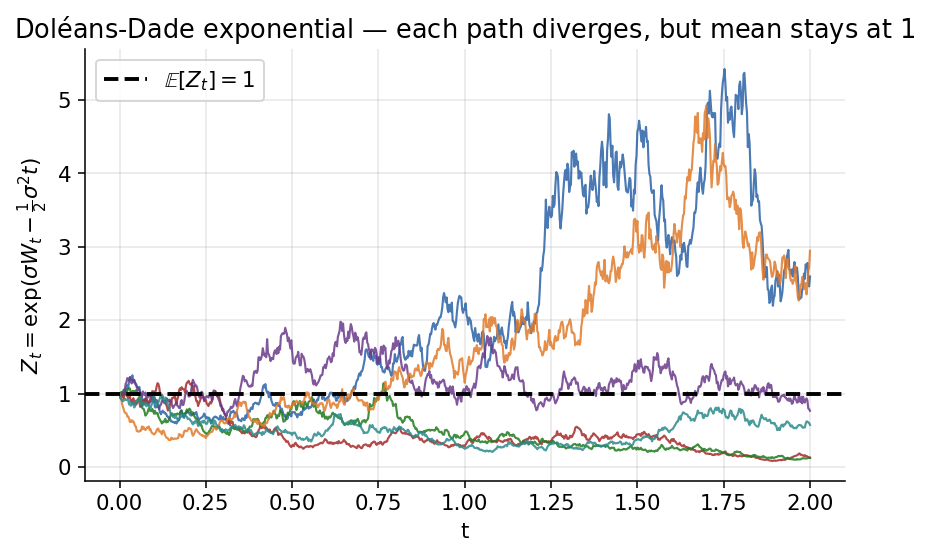
\includegraphics[keepaspectratio]{figures/ch03-doleans-dade.png}}
\emph{Six sample paths of
\(Z_t = \exp(\sigma W_t - \tfrac12\sigma^2 t)\) with \(\sigma = 0.9\).
Individual trajectories span orders of magnitude --- some rocket upward,
others drift toward zero --- yet \(\mathbb{E}[Z_t] = 1\) for every
\(t\). The \(-\tfrac12\sigma^2 t\) drift is precisely the Itô correction
that keeps the process a martingale despite its wildly dispersed paths.}

\begin{center}\rule{0.5\linewidth}{0.5pt}\end{center}

\section{3.9 Itô's Lemma for General Itô
Processes}\label{ituxf4s-lemma-for-general-ituxf4-processes}

The lemma in §3.8 handled \(X_t = f(t, W_t)\) where the underlying
process was BM itself. In practice one usually wants to transform a
diffusion with non-trivial drift and diffusion coefficients --- a GBM,
an OU process, a general Itô process. The extension is mechanical and is
called \textbf{Itô's Lemma III} in the chapter's internal numbering.

\subsection{3.9.1 Setup}\label{setup-1}

Let \(X_t\) be an Itô process satisfying

\[
\mathrm{d}X_t \;=\; \mu(t, X_t)\,\mathrm{d}t \;+\; \sigma(t, X_t)\,\mathrm{d}W_t,
\tag{3.46}
\]

for adapted drift \(\mu\) and diffusion \(\sigma\) (possibly functions
of \(t\) and \(X_t\)). Let \(g \in C^{1,2}\) and define
\(Y_t = g(t, X_t)\). Then

\[
\boxed{\;\mathrm{d}Y_t \;=\; \alpha(t, X_t)\,\mathrm{d}t \;+\; \beta(t, X_t)\,\mathrm{d}W_t\;},
\]

where

\[
\begin{aligned}
\alpha(t, x) &\;=\; \partial_t g(t, x) \;+\; \mu(t, x)\,\partial_x g(t, x) \;+\; \tfrac12\,\sigma^2(t, x)\,\partial_{xx} g(t, x), \\
\beta(t, x) &\;=\; \sigma(t, x)\,\partial_x g(t, x).
\end{aligned}
\tag{3.47}
\]

Equivalently, in the compact ``derivative-free'' form,

\[
\mathrm{d}g(t, X_t) \;=\; \partial_t g\,\mathrm{d}t \;+\; \partial_x g\,\mathrm{d}X_t \;+\; \tfrac12\,\partial_{xx} g\,(\mathrm{d}X_t)^2,
\tag{3.48}
\]

with the Itô multiplication rules (3.20), implying
\((\mathrm{d}X_t)^2 = \sigma^2(t, X_t)\,\mathrm{d}t\). The derivation is
a simple extension of the BM case: use
\((\mathrm{d}X_t)^2 = \sigma^2\,\mathrm{d}t\) in the Taylor expansion
and keep first-order terms. The result is the BM Itô formula with two
substitutions: the drift of \(X\) becomes \(\mu\) (instead of zero), and
the diffusion of \(X\) becomes \(\sigma\) (instead of one).

\textbf{Consistency with the BM case.} Setting \(\mu = 0\) and
\(\sigma = 1\) in (3.47) recovers (3.41) exactly --- so Lemma III is a
genuine generalisation, not a rewrite. Setting additionally
\(\partial_t g = 0\) recovers the time-independent version. The three
levels of generality --- \(f(W_t)\), \(f(t, W_t)\), \(g(t, X_t)\) ---
form a hierarchy of increasing scope; everything in the later chapters
uses the most general form (3.47).

\subsection{3.9.2 Cross-variation and multi-factor
Itô}\label{cross-variation-and-multi-factor-ituxf4}

If \(X_t\) and \(Y_t\) are two Itô processes driven by the same or
correlated Brownian motions, their cross-variation
\(\mathrm{d}X_t\,\mathrm{d}Y_t\) is computed by multiplying out the SDEs
and applying the Itô rules. For independent BMs \(W^1, W^2\), the rule
is \(\mathrm{d}W^1\,\mathrm{d}W^2 = 0\); for correlated BMs with
instantaneous correlation \(\rho\),
\(\mathrm{d}W^1\,\mathrm{d}W^2 = \rho\,\mathrm{d}t\). This is how
multi-factor models handle cross-terms in stochastic integrals --- each
pair of driving noises contributes its own cross-variation rate.

Itô's lemma for functions of two Itô processes is then

\[
\mathrm{d}f(t, X_t, Y_t) = \partial_t f\,\mathrm{d}t + \partial_x f\,\mathrm{d}X_t + \partial_y f\,\mathrm{d}Y_t + \tfrac12\partial_{xx}f\,(\mathrm{d}X)^2 + \partial_{xy}f\,\mathrm{d}X\,\mathrm{d}Y + \tfrac12\partial_{yy}f\,(\mathrm{d}Y)^2.
\tag{3.49}
\]

Every instance of ``two risk factors interact'' in derivatives pricing
--- quanto options, dual-currency bonds, baskets, stochastic-vol Heston
--- is an application of (3.49). We will meet these explicitly in
Chapter 8 (Margrabe exchange options) and Chapter 10 (Heston).

\begin{center}\rule{0.5\linewidth}{0.5pt}\end{center}

\section{3.10 SDE Catalogue}\label{sde-catalogue}

With Itô's lemma in hand we now solve the three canonical SDEs that
every later chapter will invoke: Geometric Brownian Motion (GBM), the
Ornstein-Uhlenbeck / Vasicek process, and the generic
constant-coefficient arithmetic SDE. Each is solved as a worked exercise
in Lemma III.

\subsection{3.10.1 Geometric Brownian Motion
(GBM)}\label{geometric-brownian-motion-gbm}

The GBM SDE is

\[
\mathrm{d}S_t \;=\; \mu\,S_t\,\mathrm{d}t \;+\; \sigma\,S_t\,\mathrm{d}W_t, \qquad S_0 \text{ given},
\tag{3.50}
\]

with constants \(\mu\) and \(\sigma > 0\). This is the dynamics assumed
for the underlying asset throughout the Black-Scholes framework (with
\(\mu\) replaced by \(r\) under the risk-neutral measure in Chapter 6).

\textbf{Solution by Itô on \(\ln S\).} Apply Lemma III with
\(g(t, s) = \ln s\) and \((\mu(t,s), \sigma(t,s)) = (\mu s, \sigma s)\).
Partial derivatives: \(\partial_t g = 0\), \(\partial_s g = 1/s\),
\(\partial_{ss} g = -1/s^2\). Plugging into (3.47):

\[
\mathrm{d}(\ln S_t) \;=\; \left[\,0 \;+\; \frac{\mu S_t}{S_t} \;+\; \tfrac12\,\sigma^2 S_t^2\cdot\!\left(\!-\frac{1}{S_t^2}\right)\right]\mathrm{d}t \;+\; \frac{\sigma S_t}{S_t}\,\mathrm{d}W_t \;=\; \left(\mu - \tfrac12\sigma^2\right)\,\mathrm{d}t \;+\; \sigma\,\mathrm{d}W_t.
\tag{3.51}
\]

The right-hand side is a constant-drift, constant-diffusion SDE --- an
arithmetic BM with drift \(\mu - \tfrac12\sigma^2\) and volatility
\(\sigma\). Integrating:

\[
\ln S_t - \ln S_0 \;=\; (\mu - \tfrac12\sigma^2)\,t \;+\; \sigma W_t,
\]

and therefore

\[
\boxed{\;S_t \;=\; S_0\,e^{(\mu - \tfrac12\sigma^2)\,t \;+\; \sigma W_t}\qquad (\text{GBM closed form})\;}.
\tag{3.52}
\]

This is the explicit closed-form solution of the GBM SDE, and it is how
every Monte Carlo simulator generates stock-price paths under the
Black-Scholes model: draw \(W_t \sim \mathcal{N}(0, t)\), plug into
(3.52), get \(S_t\). There is no time-discretisation error in this exact
scheme; the only error is the Gaussian approximation of \(W_t\), which
is \emph{exact} on any finite time horizon.

\textbf{Expected value.} Using
\(\mathbb{E}[e^{\sigma W_t}] = e^{\sigma^2 t/2}\),

\[
\mathbb{E}[S_t] \;=\; S_0\,e^{(\mu - \tfrac12\sigma^2)t}\cdot e^{\tfrac12\sigma^2 t} \;=\; S_0\,e^{\mu t}.
\tag{3.53}
\]

The expected continuously-compounded return is \(\mu\),
\emph{irrespective of} \(\sigma\). Volatility leaves the expected
forward value unchanged but does shift the median and all other
quantiles of the log-normal distribution. The risk-neutral valuation of
derivatives exploits this by ensuring \(\mu = r\) (the risk-free rate)
under \(\mathbb{Q}\), so \(\mathbb{E}^{\mathbb{Q}}[S_t] = S_0\,e^{rt}\)
--- the cost of carrying the stock equals the riskless growth rate.

\textbf{The \(-\tfrac12\sigma^2\) correction is not optional.} A common
mistake is to apply separation of variables to (3.50): write
\(\mathrm{d}S/S = \mu\,\mathrm{d}t + \sigma\,\mathrm{d}W\) and integrate
both sides to get \(\ln S_t = \ln S_0 + \mu t + \sigma W_t\),
i.e.~\(S_t = S_0 e^{\mu t + \sigma W_t}\). This is \emph{wrong}. The
chain rule \(\mathrm{d}(\ln S) = \mathrm{d}S/S\) does not hold for SDEs;
Itô's lemma tells us it is
\(\mathrm{d}(\ln S) = \mathrm{d}S/S - \tfrac12(\mathrm{d}S)^2/S^2 = \mathrm{d}S/S - \tfrac12\sigma^2\,\mathrm{d}t\).
The missing \(-\tfrac12\sigma^2\,\mathrm{d}t\) piece is the Itô
correction, and forgetting it produces
\(\mathbb{E}[S_t] = S_0 e^{\mu t + \sigma^2 t/2}\) --- which violates
the martingale property of the discounted stock (when \(\mu = r\)). The
\(-\tfrac12\sigma^2\) in (3.52) is precisely what restores the
martingale property.

\subsection{\texorpdfstring{3.10.1a Jensen's gap --- where the
\(\sigma^2/2\) really comes
from}{3.10.1a Jensen's gap --- where the \textbackslash sigma\^{}2/2 really comes from}}\label{a-jensens-gap-where-the-sigma22-really-comes-from}

The \(-\tfrac12\sigma^2 t\) in the GBM log-drift is the Jensen gap. For
convex \(f\),

\[
\mathbb{E}[f(X)] \;\geq\; f(\mathbb{E}[X]), \qquad \text{(equality iff $f$ affine or $X$ constant)}. \tag{3.52a}
\]

Concave \(f\) flips. Apply \(f = \exp\) to
\(L_t = \ln(S_t/S_0) \sim \mathcal{N}((\mu - \tfrac12\sigma^2)t, \sigma^2 t)\):

\[
\mathbb{E}[L_t] \;=\; \bigl(\mu - \tfrac12\sigma^2\bigr)t. \tag{3.52b}
\]

The MGF gives

\[
\mathbb{E}[S_t/S_0] \;=\; \mathbb{E}[e^{L_t}] \;=\; \exp\!\Bigl(\mathbb{E}[L_t] + \tfrac12\,\mathrm{Var}(L_t)\Bigr) \;=\; e^{\mu t}, \tag{3.52c}
\]

so

\[
\boxed{\;\underbrace{\ln \mathbb{E}[S_t/S_0]}_{=\;\mu t} \;-\; \underbrace{\mathbb{E}[\ln(S_t/S_0)]}_{=\;(\mu - \tfrac12\sigma^2)t} \;=\; \tfrac12\sigma^2 t\;}. \tag{3.52d}
\]

The Itô correction is the same gap, viewed from the SDE side.

\textbf{Numeric.} \(\mu = 8\%\), \(\sigma = 30\%\), \(T = 1\):

{\def\LTcaptype{none} % do not increment counter
\begin{longtable}[]{@{}lll@{}}
\toprule\noalign{}
Quantity & Formula & Value \\
\midrule\noalign{}
\endhead
\bottomrule\noalign{}
\endlastfoot
Arithmetic mean & \(e^{\mu T}\) & \(1.0833\) \\
Geometric mean & \(e^{(\mu - \sigma^2/2)T}\) & \(1.0356\) \\
Jensen gap & \(\tfrac12\sigma^2 T\) & \(0.0450\) \\
\(\ln\)(arith/geom) & \(\ln(1.0833/1.0356)\) & \(0.0450\) ✓ \\
\end{longtable}
}

A fund quoting 12\% expected return at 30\% vol delivers a long-run CAGR
closer to \(12\% - \tfrac12(30\%)^2 = 7.5\%\). Whether \(\sigma^2/2\)
appears in a pricing formula depends entirely on whether you are
computing \(\mathbb{E}[\ln S]\) or \(\ln \mathbb{E}[S]\).

\subsection{3.10.2 Ornstein-Uhlenbeck /
Vasicek}\label{ornstein-uhlenbeck-vasicek}

The OU SDE --- also known as the Vasicek short-rate equation when
applied to interest rates --- is

\[
\mathrm{d}r_t \;=\; \kappa(\theta - r_t)\,\mathrm{d}t \;+\; \sigma\,\mathrm{d}W_t, \qquad r_0 \text{ given},
\tag{3.54}
\]

with constants \(\kappa > 0\) (mean-reversion speed), \(\theta\)
(long-run mean), and \(\sigma\) (volatility). The drift
\(\kappa(\theta - r_t)\) pulls \(r_t\) toward \(\theta\) at rate
\(\kappa\); the diffusion is constant and Gaussian. This is the simplest
mean-reverting SDE and serves as the workhorse short-rate model in
Chapter 12.

\textbf{Solution by integrating factor.} The drift is linear in \(r_t\),
which suggests the integrating-factor technique familiar from linear
first-order ODEs. Multiply both sides of (3.54) by \(e^{\kappa t}\) and
recognise the left-hand side as an exact differential:

\[
\mathrm{d}(e^{\kappa t}\,r_t) \;=\; e^{\kappa t}\,\mathrm{d}r_t \;+\; \kappa\,e^{\kappa t}\,r_t\,\mathrm{d}t \;=\; e^{\kappa t}\bigl(\kappa\theta\,\mathrm{d}t + \sigma\,\mathrm{d}W_t\bigr),
\]

where the second equality substitutes (3.54) after the cancellation
\(-\kappa r_t + \kappa r_t = 0\). Integrating from \(0\) to \(t\):

\[
e^{\kappa t}\,r_t - r_0 \;=\; \kappa\theta\int_0^t e^{\kappa u}\,\mathrm{d}u \;+\; \sigma\int_0^t e^{\kappa u}\,\mathrm{d}W_u \;=\; \theta(e^{\kappa t} - 1) \;+\; \sigma\int_0^t e^{\kappa u}\,\mathrm{d}W_u.
\]

Multiplying through by \(e^{-\kappa t}\):

\[
\boxed{\;r_t \;=\; r_0 e^{-\kappa t} \;+\; \theta\bigl(1 - e^{-\kappa t}\bigr) \;+\; \sigma\int_0^t e^{-\kappa(t-u)}\,\mathrm{d}W_u\;}.
\tag{3.55}
\]

The integrating-factor step can also be verified as an Itô-lemma
computation: apply Lemma III with \(g(t, r) = e^{\kappa t}\,r\), compute
\(\partial_t g = \kappa e^{\kappa t}\,r\),
\(\partial_r g = e^{\kappa t}\), \(\partial_{rr} g = 0\), and substitute
into (3.47). The result
\(\mathrm{d}(e^{\kappa t}r_t) = e^{\kappa t}\bigl(\kappa\theta\,\mathrm{d}t + \sigma\,\mathrm{d}W_t\bigr)\)
matches the integrating-factor derivation --- a clean example of Lemma
III in action.

\textbf{Distribution of \(r_t\).} The stochastic integral in (3.55) is a
linear combination of Gaussian increments, so \(r_t\) is itself
Gaussian. Its mean is the deterministic relaxation

\[
\mathbb{E}[r_t] \;=\; r_0 e^{-\kappa t} \;+\; \theta(1 - e^{-\kappa t}),
\tag{3.56}
\]

which starts at \(r_0\) and relaxes exponentially to \(\theta\) as
\(t\to\infty\). The variance follows from the Itô isometry (3.29):

\[
\mathrm{Var}[r_t] \;=\; \sigma^2\int_0^t e^{-2\kappa(t-u)}\,\mathrm{d}u \;=\; \frac{\sigma^2}{2\kappa}\!\left(1 - e^{-2\kappa t}\right).
\tag{3.57}
\]

Two limits. As \(t \to \infty\),
\(\mathrm{Var}[r_t] \to \sigma^2/(2\kappa)\) --- mean reversion caps
variance at a finite value. As \(t \downarrow 0\),
\(\mathrm{Var}[r_t] \to \sigma^2 t\) --- over short horizons OU looks
like BM. Every mean-reverting model shares this transient-widening,
long-run-stationary pattern.

The integrated rate \(\int_0^T r_u\,\mathrm{d}u\), needed for bond
pricing in Chapter 12, is also Gaussian --- as a linear functional of
the Gaussian process \(r_t\) --- and its mean and variance are computed
by the same Fubini / Itô-isometry combination. We defer the explicit
formula to Chapter 12 where it is put to work.

\pandocbounded{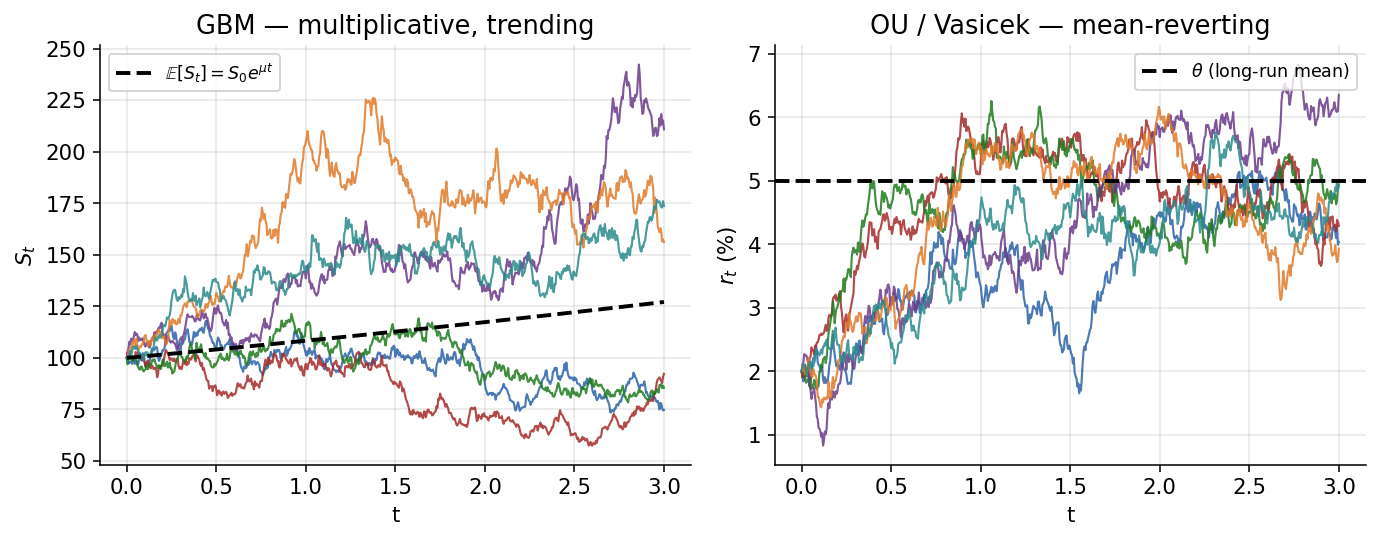
\includegraphics[keepaspectratio]{figures/ch03-ou-vs-gbm.png}}
\emph{Side-by-side comparison of the two workhorse SDEs. \textbf{Left:}
GBM paths trend exponentially with multiplicative noise; the mean curve
\(S_0 e^{\mu t}\) grows without bound. \textbf{Right:} OU / Vasicek
paths wobble around the long-run mean \(\theta\); variance saturates at
\(\sigma^2/(2\kappa)\) so the ensemble never escapes. Mean-reversion is
visually unmistakable.}

\begin{figure}
\centering
\pandocbounded{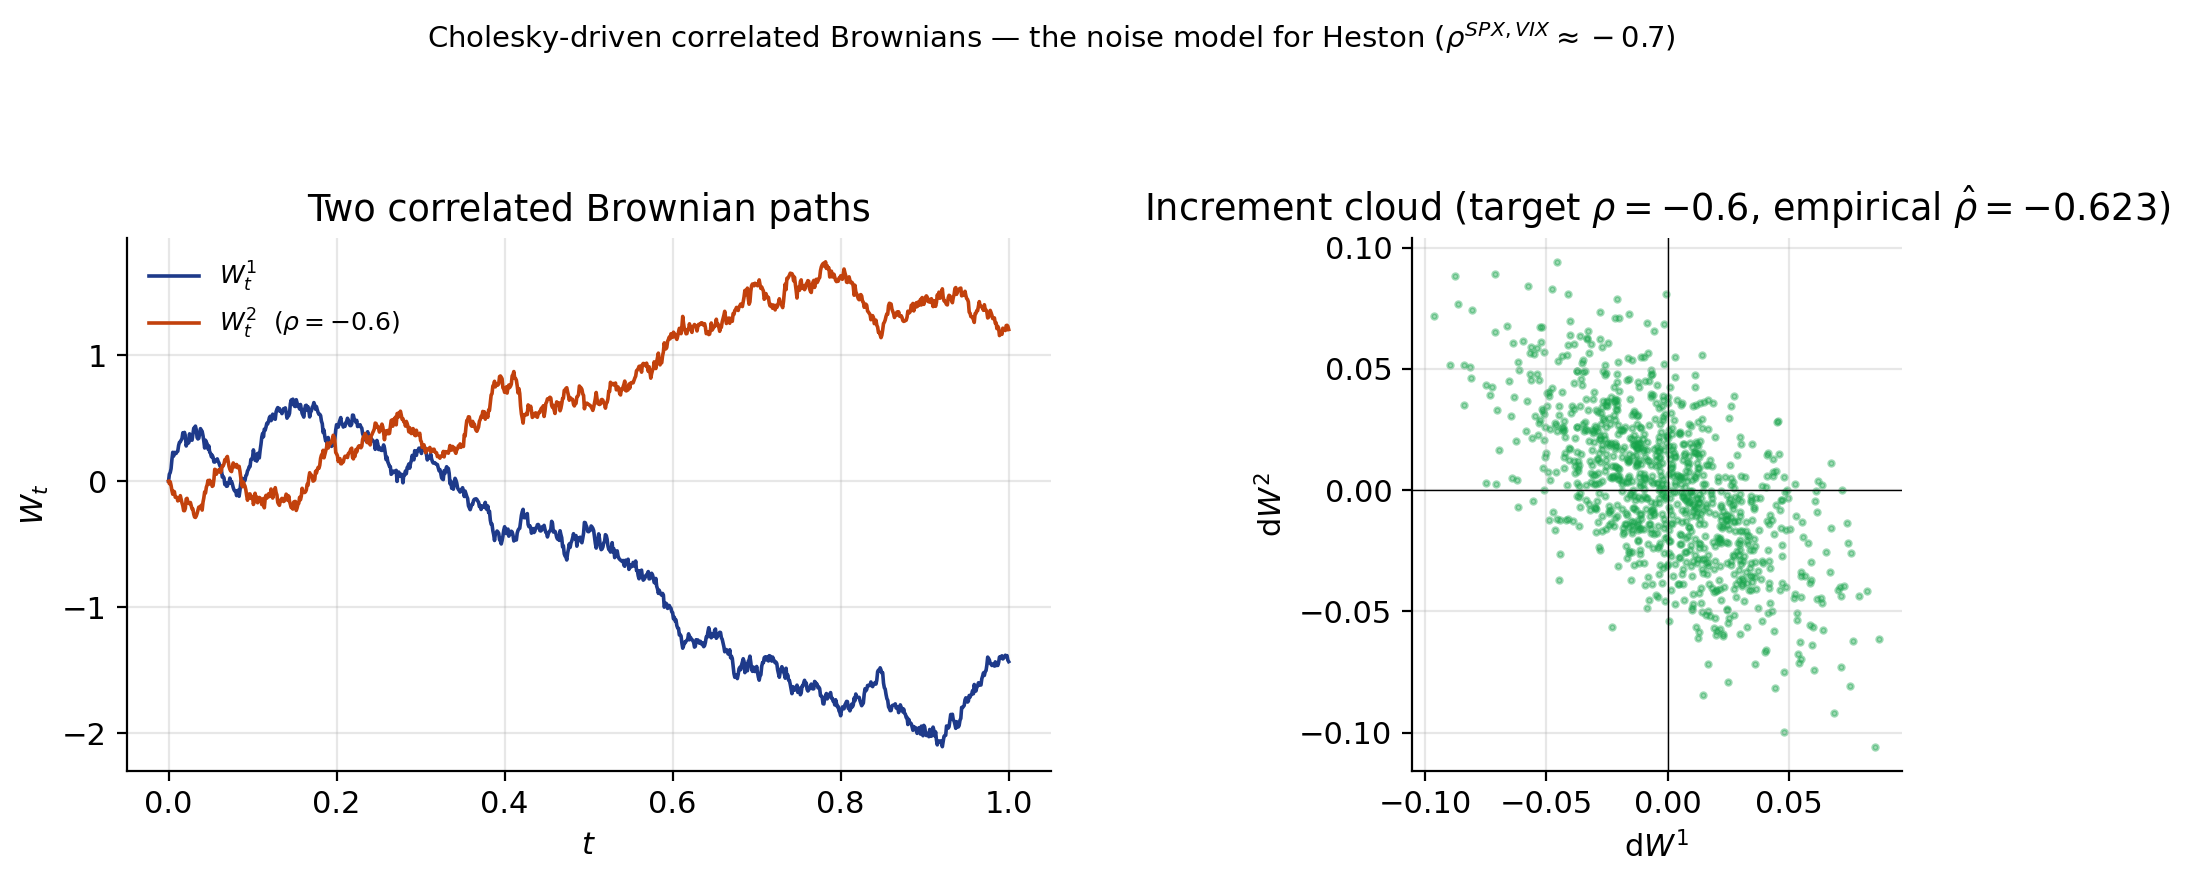
\includegraphics[keepaspectratio]{figures/ch03-sde-correlated.png}}
\caption{Two correlated Brownian motions generated via Cholesky
\(L=[1,0;\rho,\sqrt{1-\rho^2}]\) at \(\rho=-0.6\), with the empirical
increment scatter recovering the target correlation. This is the noise
structure of Heston, where \(\rho^{SPX,\sqrt{v}} \approx -0.7\) since
2010 (Ch. 10's empirical chapter appendix)}
\end{figure}

\subsection{3.10.3 Constant-coefficient arithmetic
BM}\label{constant-coefficient-arithmetic-bm}

The simplest possible SDE --- no state-dependence in either drift or
diffusion --- is

\[
\mathrm{d}X_t \;=\; a\,\mathrm{d}t \;+\; b\,\mathrm{d}W_t, \qquad X_0 \text{ given},
\tag{3.58}
\]

with constants \(a\) and \(b\). Because the coefficients do not depend
on \(X_t\), direct integration works without any transformation:

\[
X_t \;=\; X_0 \;+\; a\,t \;+\; b\,W_t.
\tag{3.59}
\]

The solution is Gaussian with mean \(X_0 + a t\) and variance \(b^2 t\).
This is the ``trivially solvable'' SDE, and its chief uses are (i) as
the reference process after Itô-transforming a more complicated SDE to
constant coefficients (e.g.~the log-GBM reduction (3.51)), and (ii) as
the Bachelier model of asset prices --- rarely used for equities but
standard in certain rates markets (notably swaption pricing with normal
volatilities, which we revisit in Chapter 14).

Arithmetic BM allows \(X_t < 0\) (Gaussian support is all of
\(\mathbb{R}\)); GBM keeps \(S_t > 0\). Equities use GBM; interest rates
(occasionally negative post-2014) use arithmetic-style models.

\subsection{3.10.3b The Brownian Bridge}\label{b-the-brownian-bridge}

A Brownian motion conditioned on its two endpoints is called a
\textbf{Brownian Bridge} and plays a starring role in barrier-option
Monte Carlo (Ch. 9), CDS calibration, and any path-conditioned
simulation. Fix \(T > 0\) and a real number \(b\). The Brownian Bridge
is the law of \(W\) on \([0, T]\) conditional on \(W_0 = 0\) and
\(W_T = b\):

\[
B_t \;:=\; (W_t \mid W_0 = 0,\, W_T = b), \qquad t \in [0, T].
\tag{3.57a}
\]

Two facts pin its distribution. The conditional mean is the
deterministic line \[
\mathbb{E}[B_t] \;=\; \frac{t}{T}\,b,
\tag{3.57b}
\] and the conditional variance is the \textbf{bridge envelope} \[
\boxed{\;\mathrm{Var}(B_t) \;=\; \frac{t\,(T - t)}{T}.\;}
\tag{3.57c}
\]

The variance vanishes at both endpoints (where the value is pinned) and
is maximal in the middle at \(t = T/2\), where
\(\mathrm{Var}(B_{T/2}) = T/4\). \emph{Intuition: at the two pins there
is zero uncertainty; the most freedom to wander is exactly halfway
between them.}

\begin{figure}
\centering
\pandocbounded{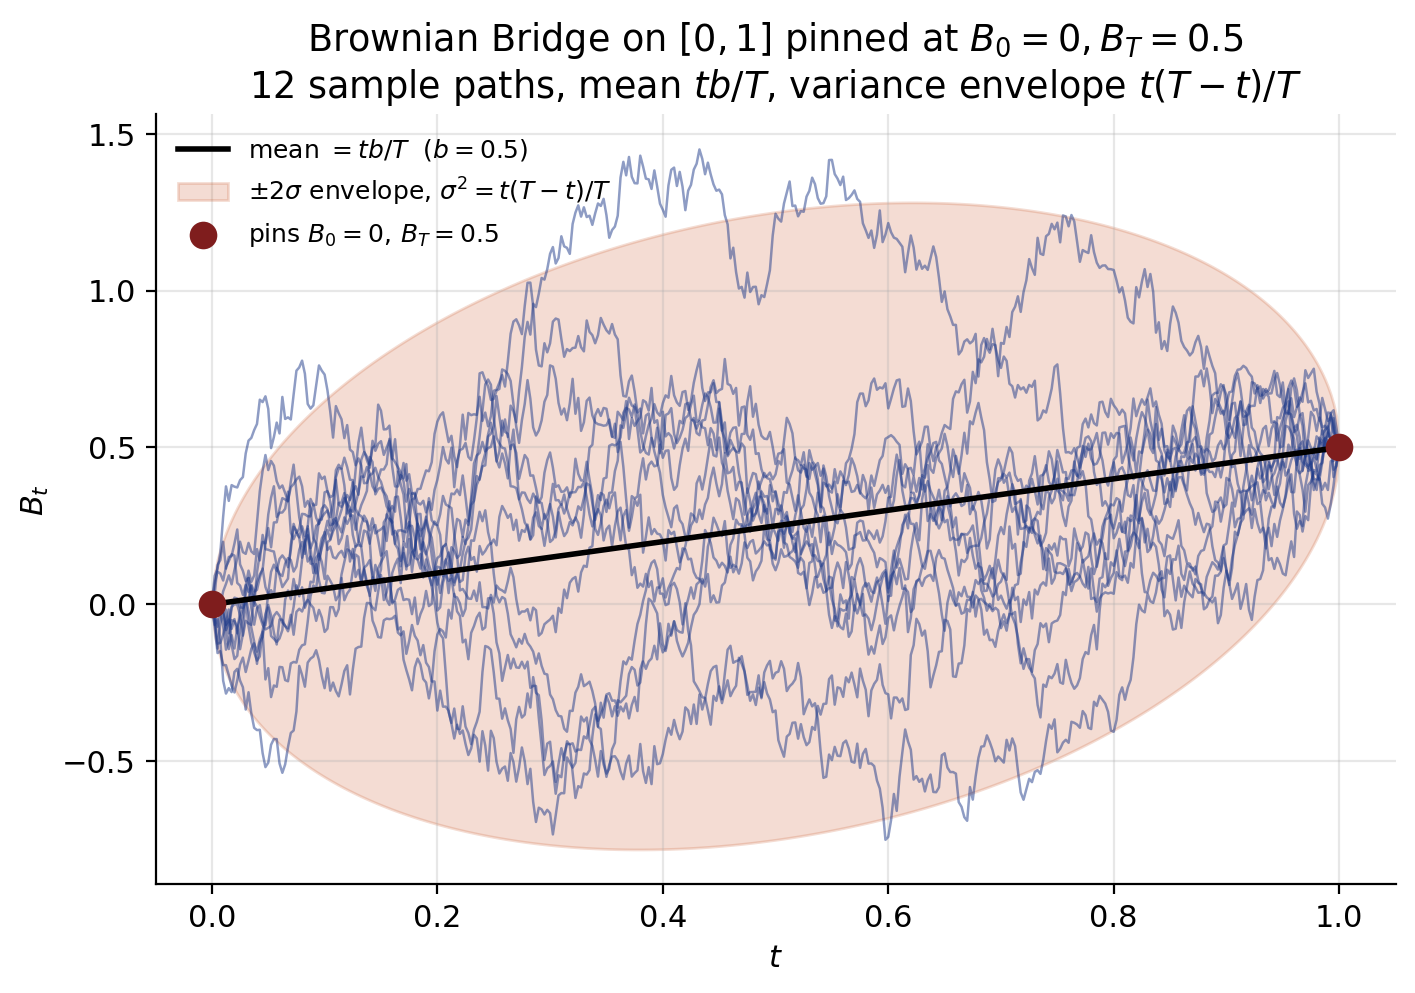
\includegraphics[keepaspectratio]{figures/ch03-bb-paths.png}}
\caption{Twelve Brownian Bridge sample paths pinned at \(B_0=0\) and
\(B_T=0.5\), with mean \(tb/T\) and the \(\pm 2\sigma\) envelope
\(t(T-t)/T\). Same construction as a daily-close path of SPX where the
open and close are fixed but the intra-day high-low range is what one is
integrating against}
\end{figure}

\textbf{Direct construction.} A Brownian Bridge can be simulated from a
free BM by the simple \textbf{bridge transformation} \[
B_t \;=\; W_t \;-\; \frac{t}{T}\,W_T \;+\; \frac{t}{T}\,b.
\tag{3.57d}
\] Verify: at \(t=0\), \(B_0 = 0\); at \(t = T\),
\(B_T = W_T - W_T + b = b\). The middle term subtracts off the realised
endpoint and the last term substitutes the desired pin --- exactly the
conditioning operation.

\textbf{SDE form.} \(B_t\) also solves a linear SDE with a drift that
grows singular at \(T\): \[
\mathrm{d}B_t \;=\; \frac{b - B_t}{T - t}\,\mathrm{d}t \;+\; \mathrm{d}W_t, \qquad B_0 = 0.
\tag{3.57e}
\] The mean-reversion to the pin \(b\) accelerates as \(t \to T\) --- a
forced landing. As a useful sanity check, the same drift pulls toward
\(tb/T\) in expectation, which is exactly (3.57b).

\begin{figure}
\centering
\pandocbounded{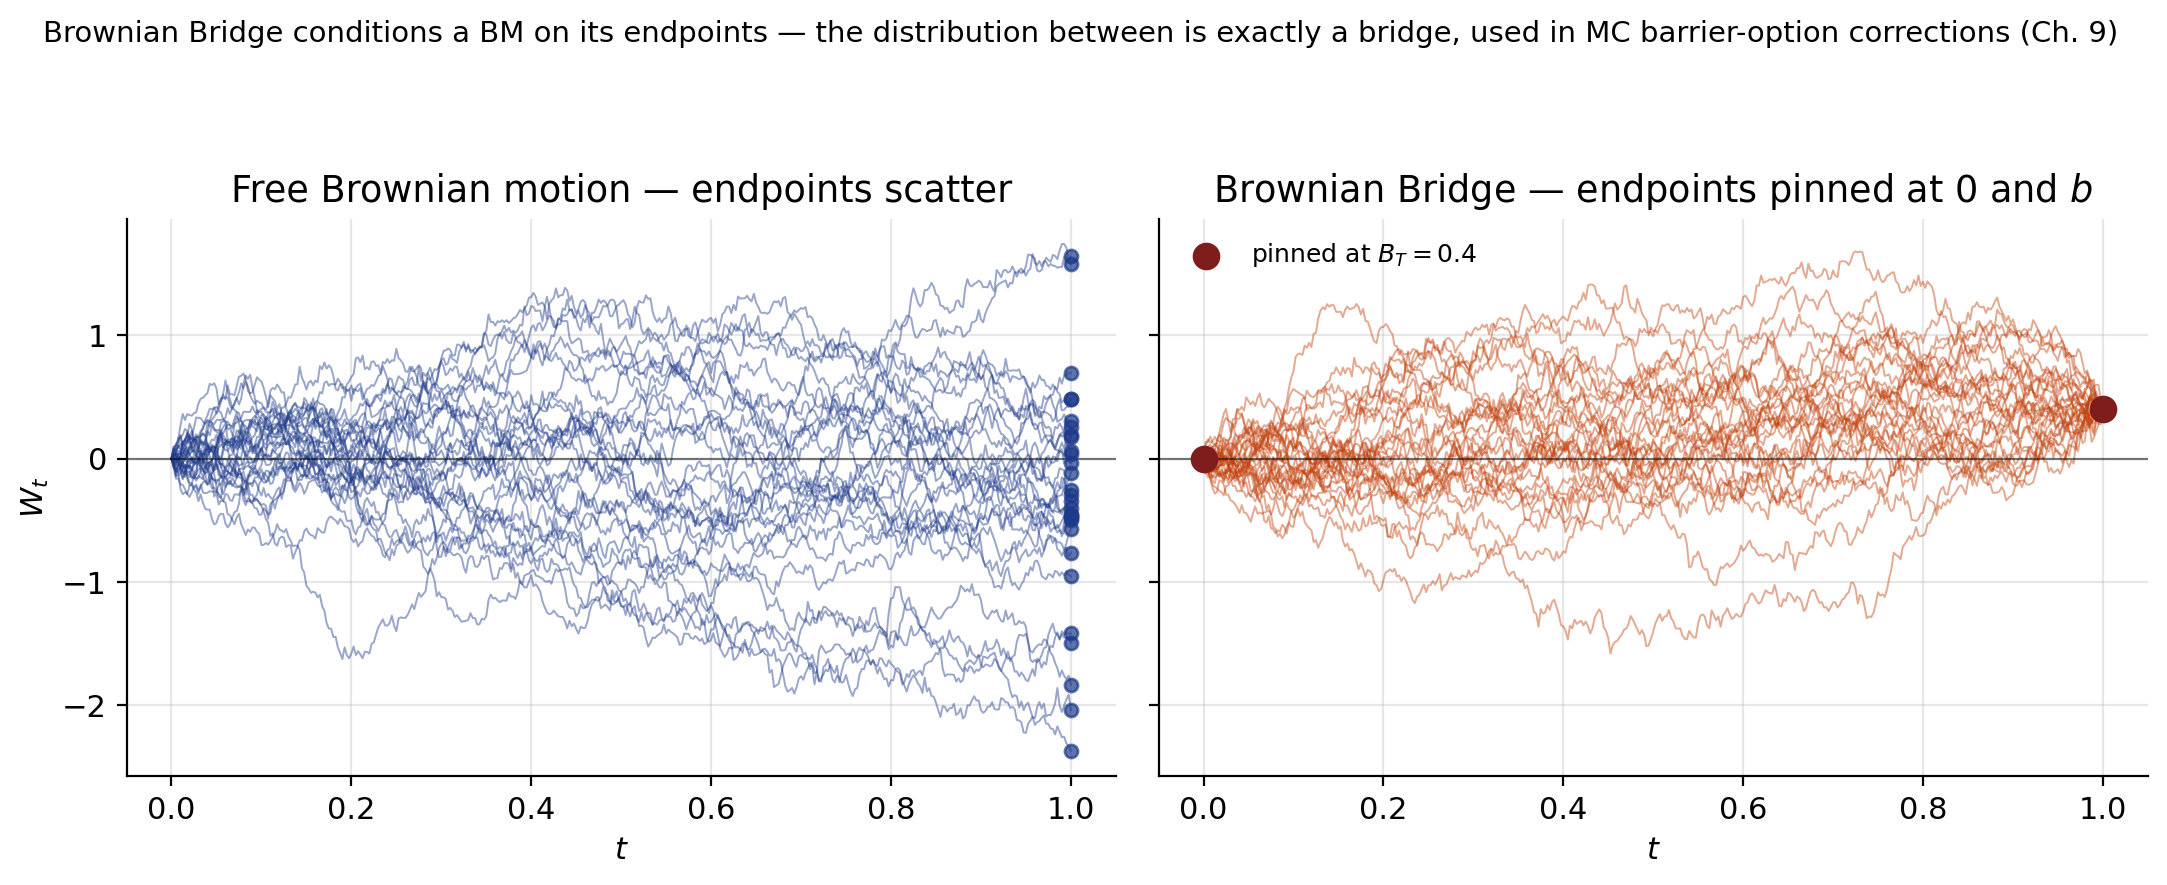
\includegraphics[keepaspectratio]{figures/ch03-bb-vs-bm.png}}
\caption{Free Brownian motion endpoints scatter freely (left) versus
Brownian Bridge endpoints pinned at \(b=0.4\) (right) --- the
conditioning that drives Monte-Carlo barrier-option corrections in Ch.
9}
\end{figure}

\textbf{Where it matters.} Beyond the Ch. 9 barrier correction, the
bridge controls (i) intra-day volatility of a daily-closed asset (open
and close are observed; the conditional max/min has bridge laws), (ii)
interpolation of yield-curve nodes between calibrated maturities, and
(iii) every ``fixed start, fixed end'' stochastic model ---
e.g.~central-bank rate paths between meetings where guidance pins the
endpoints.

\subsection{3.10.4 Summary of solved SDEs}\label{summary-of-solved-sdes}

{\def\LTcaptype{none} % do not increment counter
\begin{longtable}[]{@{}
  >{\raggedright\arraybackslash}p{(\linewidth - 4\tabcolsep) * \real{0.3333}}
  >{\raggedright\arraybackslash}p{(\linewidth - 4\tabcolsep) * \real{0.3333}}
  >{\raggedright\arraybackslash}p{(\linewidth - 4\tabcolsep) * \real{0.3333}}@{}}
\toprule\noalign{}
\begin{minipage}[b]{\linewidth}\raggedright
SDE
\end{minipage} & \begin{minipage}[b]{\linewidth}\raggedright
Solution
\end{minipage} & \begin{minipage}[b]{\linewidth}\raggedright
Distribution of \(X_t\)
\end{minipage} \\
\midrule\noalign{}
\endhead
\bottomrule\noalign{}
\endlastfoot
\(\mathrm{d}S_t = \mu S_t\,\mathrm{d}t + \sigma S_t\,\mathrm{d}W_t\)
(GBM) & \(S_t = S_0\,e^{(\mu - \tfrac12\sigma^2)t + \sigma W_t}\) &
Log-normal \\
\(\mathrm{d}r_t = \kappa(\theta - r_t)\,\mathrm{d}t + \sigma\,\mathrm{d}W_t\)
(OU) &
\(r_t = r_0 e^{-\kappa t} + \theta(1-e^{-\kappa t}) + \sigma\!\int_0^t e^{-\kappa(t-u)}\,\mathrm{d}W_u\)
& Gaussian \\
\(\mathrm{d}X_t = a\,\mathrm{d}t + b\,\mathrm{d}W_t\) (arithmetic BM) &
\(X_t = X_0 + a t + b W_t\) & Gaussian \\
\end{longtable}
}

Every SDE encountered in the rest of the guide either is one of these
three or reduces to one by an Itô transformation. The Heston
stochastic-volatility model of Chapter 10 is one partial exception (the
variance process is CIR, which requires a Bessel-process argument we
develop there), but even it uses OU-like integrating-factor ideas on the
variance term.

\begin{center}\rule{0.5\linewidth}{0.5pt}\end{center}

\section{3.11 Worked Stochastic
Integrals}\label{worked-stochastic-integrals}

A small library of stochastic integrals later chapters invoke. The
recipe for any \(\int_0^t g(s, W_s)\,\mathrm{d}W_s\):

\begin{enumerate}
\def\labelenumi{\arabic{enumi}.}
\tightlist
\item
  Choose a candidate \(f(t, w)\) such that
  \(\partial_w f(t, w) = g(t, w)\).
\item
  Compute the Itô differential \(\mathrm{d}f(t, W_t)\) using (3.41).
\item
  Integrate from \(0\) to \(t\) and solve for the stochastic integral:
  \[\int_0^t g(s, W_s)\,\mathrm{d}W_s = f(t, W_t) - f(0, 0) - \int_0^t [\partial_s f + \tfrac12\partial_{ww}f]\,\mathrm{d}s.\]
\end{enumerate}

The right-hand side is pathwise --- a mix of terminal-value evaluations
and ordinary Riemann integrals. The stochastic integral has been
\emph{reduced} to these ingredients. That is the whole trick.

\subsection{\texorpdfstring{3.11.1 A stochastic integration-by-parts:
\(\int_0^t s\,W_s\,\mathrm{d}W_s\)}{3.11.1 A stochastic integration-by-parts: \textbackslash int\_0\^{}t s\textbackslash,W\_s\textbackslash,\textbackslash mathrm\{d\}W\_s}}\label{a-stochastic-integration-by-parts-int_0t-sw_smathrmdw_s}

Consider the product \(X_t = t\,W_t^2\), i.e.~take \(f(t, w) = t\,w^2\).
Partials: \(\partial_t f = w^2\), \(\partial_w f = 2 t w\),
\(\partial_{ww} f = 2 t\). Plugging into (3.41):

\[
\mathrm{d}(t\,W_t^2) \;=\; \bigl[\,W_t^2 \;+\; t\,\bigr]\,\mathrm{d}t \;+\; 2 t\,W_t\,\mathrm{d}W_t.
\tag{3.60}
\]

Integrating from \(0\) to \(t\) with \(X_0 = 0\):

\[
t\,W_t^2 \;=\; \int_0^t \bigl(W_s^2 + s\bigr)\,\mathrm{d}s \;+\; \int_0^t 2 s\,W_s\,\mathrm{d}W_s,
\]

so that

\[
\boxed{\;\int_0^t 2\,s\,W_s\,\mathrm{d}W_s \;=\; t\,W_t^2 \;-\; \int_0^t W_s^2\,\mathrm{d}s \;-\; \tfrac12 t^2\;}.
\tag{3.61}
\]

This is a stochastic integration-by-parts identity for \(s\,W_s\): the
product of a deterministic function of \(s\) and a Brownian function is
expressible in terms of the terminal product plus ordinary pathwise
integrals. A sanity check: taking expectations on both sides, the
left-hand side is \(0\) (martingale), and the right-hand side is
\(\mathbb{E}[tW_t^2] - \int_0^t s\,\mathrm{d}s - \tfrac12 t^2 = t\cdot t - \tfrac12 t^2 - \tfrac12 t^2 = 0\).
✓

More generally, for any \(f(t, w) = \phi(t)\,\psi(w)\) product form,
Itô's lemma gives the analogue of the ordinary product rule with an Itô
correction:

\[
\mathrm{d}(\phi(t)\,\psi(W_t)) \;=\; \phi'(t)\,\psi(W_t)\,\mathrm{d}t \;+\; \phi(t)\,\psi'(W_t)\,\mathrm{d}W_t \;+\; \tfrac12\,\phi(t)\,\psi''(W_t)\,\mathrm{d}t.
\tag{3.62}
\]

\subsection{\texorpdfstring{3.11.2 Integration-by-parts for
\(\int_0^t s\,e^{W_s}\,\mathrm{d}W_s\)}{3.11.2 Integration-by-parts for \textbackslash int\_0\^{}t s\textbackslash,e\^{}\{W\_s\}\textbackslash,\textbackslash mathrm\{d\}W\_s}}\label{integration-by-parts-for-int_0t-sew_smathrmdw_s}

Take \(f(t, w) = t\,e^{w}\), chosen so that \(\partial_w f = t\,e^w\)
--- almost the desired \(s\,e^{W_s}\), but with \(t\) frozen rather than
integrated. Partials: \(\partial_t f = e^w\), \(\partial_w f = t\,e^w\),
\(\partial_{ww} f = t\,e^w\). Itô:

\[
\mathrm{d}(t\,e^{W_t}) \;=\; \bigl[\,e^{W_t} \;+\; \tfrac12\,t\,e^{W_t}\,\bigr]\,\mathrm{d}t \;+\; t\,e^{W_t}\,\mathrm{d}W_t.
\tag{3.63}
\]

Integrating \(0\to t\) and rearranging,

\[
\boxed{\;\int_0^t s\,e^{W_s}\,\mathrm{d}W_s \;=\; t\,e^{W_t} \;-\; \int_0^t e^{W_s}\,\mathrm{d}s \;-\; \tfrac12\int_0^t s\,e^{W_s}\,\mathrm{d}s\;}.
\tag{3.64}
\]

The answer decomposes into a terminal-value algebraic piece and two
pathwise Riemann integrals. Neither pathwise integral has a simpler
closed form, but both are perfectly tractable for Monte Carlo simulation
or moment calculations. The stochastic integral
\(\int_0^t s e^{W_s}\,\mathrm{d}W_s\) itself is a martingale with
variance
\(\int_0^t s^2\,\mathbb{E}[e^{2W_s}]\,\mathrm{d}s = \int_0^t s^2 e^{2s}\,\mathrm{d}s\)
by Itô isometry. This is the template for every ``polynomial-in-\(s\)
times exponential-in-\(W_s\)'' integral that appears downstream.

\subsection{3.11.3 A catalogue of Brownian
computations}\label{a-catalogue-of-brownian-computations}

The following compact list summarises the moments that will be reused
without re-derivation:

\[
\mathbb{E}[W_t] = 0, \qquad \mathrm{Var}[W_t] = t, \qquad \mathbb{E}[W_t^4] = 3t^2,
\]

\[
\mathbb{E}[W_s W_t] = \min(s,t), \qquad \mathrm{Var}[W_t^2] = 2 t^2,
\]

\[
\mathbb{E}[e^{\sigma W_t}] = e^{\tfrac12\sigma^2 t}, \qquad \mathbb{E}[e^{-\tfrac12\sigma^2 t + \sigma W_t}] = 1,
\]

\[
\mathrm{Var}\!\left[\int_0^t g_s\,\mathrm{d}W_s\right] = \int_0^t \mathbb{E}[g_s^2]\,\mathrm{d}s,
\]

\[
\mathrm{Var}\!\left[\int_0^t W_s\,\mathrm{d}s\right] = \tfrac13 t^3.
\]

Every one of these is either a direct MGF exercise or a one-line
Itô-isometry application. None will be re-derived in later chapters.

\begin{center}\rule{0.5\linewidth}{0.5pt}\end{center}

\section{3.12 Chapter Summary}\label{chapter-summary}

Established:

\begin{itemize}
\tightlist
\item
  \textbf{Brownian motion} is the continuum limit of a symmetric scaled
  random walk with \(\sqrt{\Delta t}\) increments. It has Gaussian
  marginals, stationary and independent increments, continuous paths ---
  properties (i)-(iv) of (3.8).
\item
  \textbf{Path properties.} BM has infinite total variation (3.14) and
  finite quadratic variation \([W,W]_t = t\) (3.19), summarised by the
  Itô rule \((\mathrm{d}W)^2 = \mathrm{d}t\) in (3.20).
\item
  \textbf{The Itô integral} \(\int_0^t g_s\,\mathrm{d}W_s\) is defined
  by left-endpoint Riemann sums (3.22). The left-endpoint choice is what
  makes it a martingale --- the mathematical encoding of no-arbitrage
  predictability.
\item
  \textbf{The Itô isometry} (3.28)-(3.29) computes the variance of any
  stochastic integral as a deterministic time integral of the squared
  integrand. It generalises \([W,W]_t = t\) from the identity to
  arbitrary integrands.
\item
  \textbf{Itô's lemma} (3.41) --- the stochastic chain rule --- carries
  an extra term \(\tfrac12\partial_{ww}f\,\mathrm{d}t\) relative to the
  classical chain rule, absent in ordinary calculus because smooth paths
  have zero QV. The general form (3.47) handles transforms of any Itô
  process.
\item
  \textbf{SDE catalogue.} GBM (3.52), OU/Vasicek (3.55), and arithmetic
  BM (3.59) are the three canonical SDEs. Every SDE encountered later
  either is one of these three or reduces to one by an Itô
  transformation.
\end{itemize}

\subsection{Key takeaways}\label{key-takeaways-2}

\begin{enumerate}
\def\labelenumi{\arabic{enumi}.}
\tightlist
\item
  \textbf{\((\mathrm{d}W)^2 = \mathrm{d}t\) is the source of every Itô
  correction.} Every time you see a \(-\tfrac12\sigma^2 t\),
  \(\tfrac12\,\sigma^2\,\partial_{xx}\), or ``convexity adjustment'' in
  a later chapter, it descends from this single identity.
\item
  \textbf{TV versus QV.} BM has infinite TV (distance) but finite QV
  (energy). The gap between them is the gamma-theta trade-off of options
  and the structural reason variance swaps replicate by log-contracts
  while ``realised-absolute-value swaps'' do not.
\item
  \textbf{Left endpoints matter.} The Itô integral's martingale property
  depends on evaluating the integrand at \(t_{k-1}\), not \(t_k\). This
  is the mathematical expression of ``predictable strategies earn zero
  expected P\&L,'' i.e.~no-arbitrage in continuous time.
\item
  \textbf{Itô's lemma is the chain rule plus curvature.} Options traders
  already know it: long-gamma books bleed theta at the rate
  \(\tfrac12\sigma^2 S^2\Gamma\), and this rate is exactly the Itô
  correction applied to the Black-Scholes price.
\item
  \textbf{Closed-form SDEs are scarce.} Only a handful of SDEs admit
  explicit solutions --- GBM, OU, linear-Gaussian, and a few others. The
  rest are solved numerically (Euler-Maruyama, Milstein) or transformed
  to a solvable form by Itô's lemma (the Lamperti transform).
\end{enumerate}

\subsection{Reference formulas}\label{reference-formulas-2}

\begin{itemize}
\tightlist
\item
  \textbf{Itô rules:} \((\mathrm{d}W)^2 = \mathrm{d}t\),
  \(\mathrm{d}W\,\mathrm{d}t = 0\), \((\mathrm{d}t)^2 = 0\).
\item
  \textbf{Itô's lemma for \(X_t = f(t, W_t)\):}
  \[\mathrm{d}X_t = \bigl[\partial_t f + \tfrac12\partial_{ww}f\bigr]\,\mathrm{d}t + \partial_w f\,\mathrm{d}W_t.\]
\item
  \textbf{Itô's lemma for \(Y_t = g(t, X_t)\) with
  \(\mathrm{d}X_t = \mu\,\mathrm{d}t + \sigma\,\mathrm{d}W_t\):}
  \[\mathrm{d}Y_t = \bigl[\partial_t g + \mu\,\partial_x g + \tfrac12\sigma^2\,\partial_{xx}g\bigr]\,\mathrm{d}t + \sigma\,\partial_x g\,\mathrm{d}W_t.\]
\item
  \textbf{Itô isometry:}
  \[\mathbb{E}\!\left[\left(\int_0^t g_s\,\mathrm{d}W_s\right)^{\!2}\right] = \mathbb{E}\!\int_0^t g_s^2\,\mathrm{d}s.\]
\item
  \textbf{GBM solution:}
  \(S_t = S_0\,e^{(\mu - \tfrac12\sigma^2)t + \sigma W_t}\).
\item
  \textbf{OU solution:}
  \(r_t = r_0 e^{-\kappa t} + \theta(1 - e^{-\kappa t}) + \sigma\int_0^t e^{-\kappa(t-u)}\,\mathrm{d}W_u\),
  with
  \(\mathrm{Var}[r_t] = \tfrac{\sigma^2}{2\kappa}(1 - e^{-2\kappa t})\).
\item
  \textbf{Exponential martingale:}
  \(\mathrm{d}(e^{-\tfrac12\sigma^2 t + \sigma W_t}) = \sigma\,e^{-\tfrac12\sigma^2 t + \sigma W_t}\,\mathrm{d}W_t\),
  driftless.
\item
  \textbf{Key Brownian moments:} \(\mathbb{E}[W_t^2] = t\),
  \(\mathbb{E}[W_t^4] = 3t^2\), \(\mathbb{E}[W_s W_t] = \min(s,t)\),
  \(\mathbb{E}[e^{\sigma W_t}] = e^{\sigma^2 t/2}\).
\end{itemize}

With these tools in hand we turn in Chapter 4 to the Feynman-Kac bridge
between SDEs and PDEs, which will hand us the Kolmogorov backward
equation and prepare the ground for the risk-neutral pricing framework
of Chapters 5-8.

\newpage

\chapter{Chapter 4 --- Feynman-Kac and the SDE-PDE
Bridge}\label{chapter-4-feynman-kac-and-the-sde-pde-bridge}

This chapter uses the Ch. 3 toolkit for its first major payoff: the
\emph{Feynman--Kac} theorem, the bidirectional bridge between a linear
parabolic PDE and the conditional expectation of a diffusion-driven
payoff. Every pricing problem in the rest of the guide ---
Black--Scholes (Ch. 6), Vasicek bonds (Ch. 12), caplets (Ch. 14) --- is
one substitution into the same template.

We establish the duality in three forms --- zero-drift BM,
constant-coefficient drifted BM with discounting, and full
state-time-dependent coefficients --- and compute three worked examples
to see the machinery turn. The Black--Scholes derivation itself is
deferred to Ch. 6 (twice: once via hedging, once as a Feynman--Kac
corollary); measure change is Ch. 5.

\section{4.1 Motivation --- Why an SDE-PDE Bridge
Matters}\label{motivation-why-an-sde-pde-bridge-matters}

Every pricing problem reduces to one of two computations: solve a
backward parabolic PDE on a space-time grid, or average a random payoff
over diffusion paths. These look like different calculations ---
finite-difference code on a mesh vs Monte Carlo on trajectories --- and
Feynman--Kac says they are the same calculation.

Routing is practical. Low-dimensional smooth problems (single-asset
vanilla, single-rate caplet) are faster via PDE --- a Crank--Nicolson
grid converges in milliseconds. High-dimensional or path-dependent
problems (baskets, exotics, multi-factor rates) are faster via Monte
Carlo --- \(1/\sqrt{N_{\text{paths}}}\) error independent of state
dimension. American features favour PDEs (exercise boundary embeds in
the grid); path-dependent features favour MC (track a functional along
the path). Feynman--Kac guarantees the answers agree.

Every linear pricing PDE in this guide --- Black--Scholes, Vasicek,
Hull--White, Heston, the caplet equations of Ch. 14 --- is a
Feynman--Kac PDE for some SDE and some discount rate. Mastering the
bridge in its full state-dependent form gives a single theorem that,
properly instantiated, prices every linear problem in the guide.

\begin{center}\rule{0.5\linewidth}{0.5pt}\end{center}

\section{4.2 The Zero-Drift Feynman-Kac
Theorem}\label{the-zero-drift-feynman-kac-theorem}

Start with driftless, undiscounted BM and a terminal payoff. Every later
version is a decoration of this base case.

Let \(X\) be a standard Brownian motion, \(T > 0\) a horizon, and
\(\varphi : \mathbb{R} \to \mathbb{R}\) a payoff with polynomial growth.
Consider the backward Cauchy problem

\[
\begin{cases}
\partial_t f(t, x) \;+\; \tfrac{1}{2}\,\partial_{xx} f(t, x) \;=\; 0, & (t, x) \in [0, T) \times \mathbb{R}, \\[2pt]
f(T, x) \;=\; \varphi(x).
\end{cases}
\tag{4.1}
\]

Feynman-Kac asserts that this PDE is \emph{equivalent} to the
probabilistic representation

\[
\boxed{\;f(t, x) \;=\; \mathbb{E}_{t, x}\!\left[\,\varphi(X_T)\,\right] \;\equiv\; \mathbb{E}\!\left[\,\varphi(X_T)\,\big|\,X_t = x\,\right].\;}
\tag{4.2}
\]

The biconditional carries both directions. \textbf{PDE \(\Rightarrow\)
expectation:} a classical solution of \((4.1)\) admits the expectation
representation \((4.2)\). \textbf{Expectation \(\Rightarrow\) PDE:}
conversely, the function \(x \mapsto \mathbb{E}_{t,x}[\varphi(X_T)]\)
automatically satisfies \((4.1)\). In practice one direction or the
other is the easier computation, and Feynman-Kac lets us freely pick.

\begin{figure}
\centering
\pandocbounded{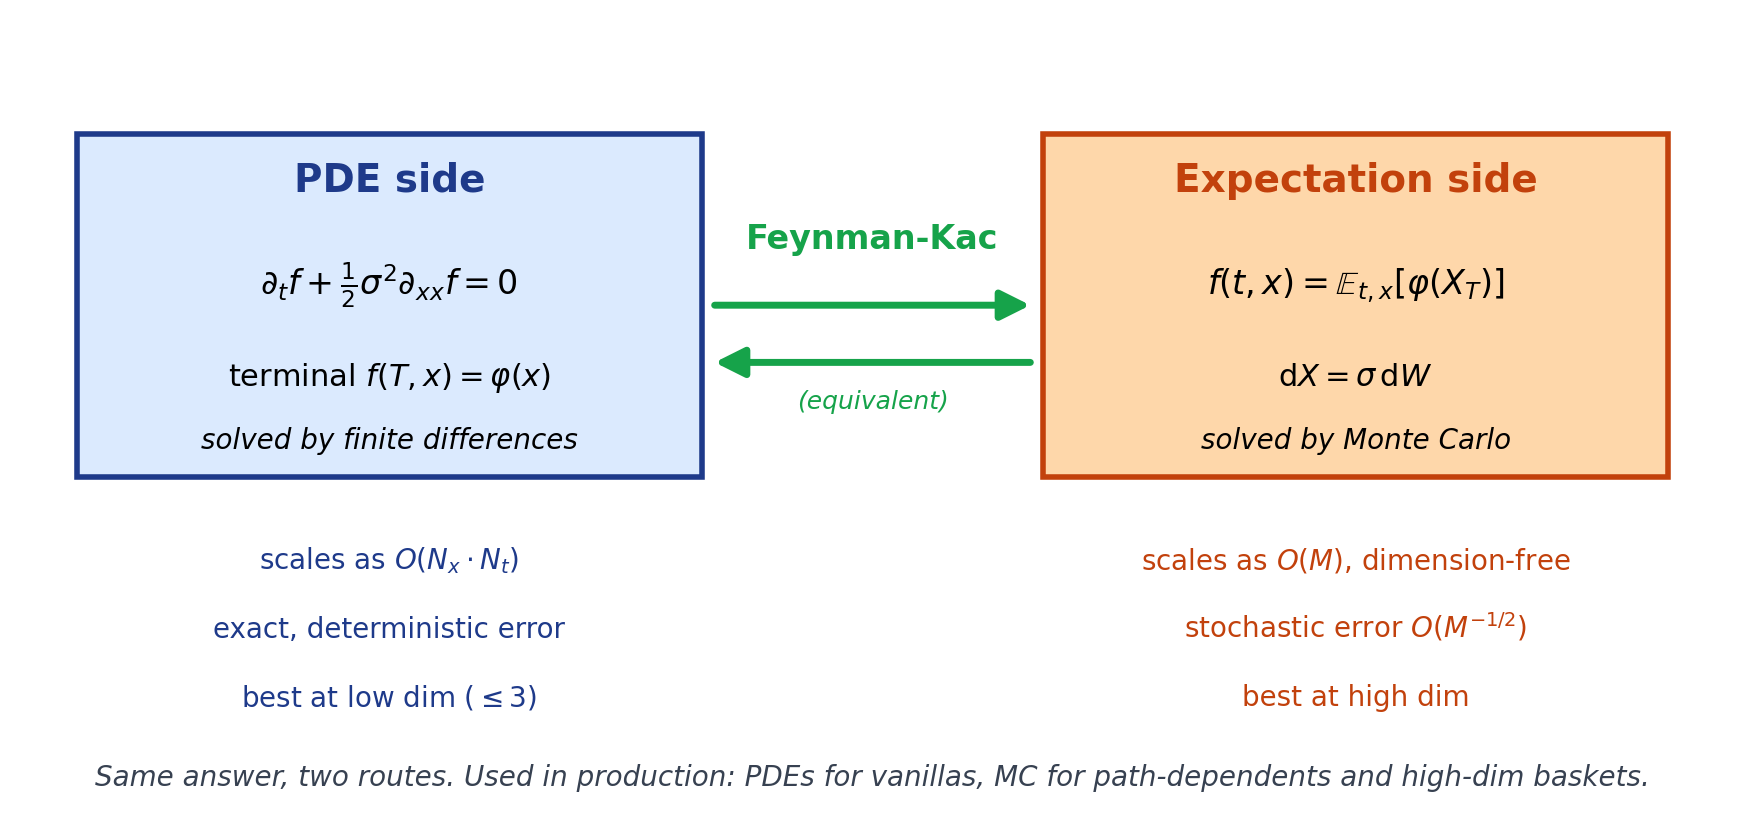
\includegraphics[keepaspectratio]{figures/ch04-pde-vs-expectation.png}}
\caption{Feynman-Kac duality: the same option price can be computed as
the solution of a backward parabolic PDE (left, finite differences) or
as a discounted risk-neutral expectation (right, Monte Carlo). Most
production vol desks run both --- PDE for vanillas, MC for
path-dependents --- and use one as a sanity check on the other}
\end{figure}

\subsection{4.2.1 What the PDE is}\label{what-the-pde-is}

The PDE in \((4.1)\) is the reverse heat equation --- the Kolmogorov
backward equation for BM. The terminal payoff plays the role of initial
heat distribution; the PDE smooths it backward from \(T\) to \(t\).
Every qualitative feature of diffusion --- smoothing of discontinuities,
exponential decay of modes --- translates directly into option-price
behaviour.

\pandocbounded{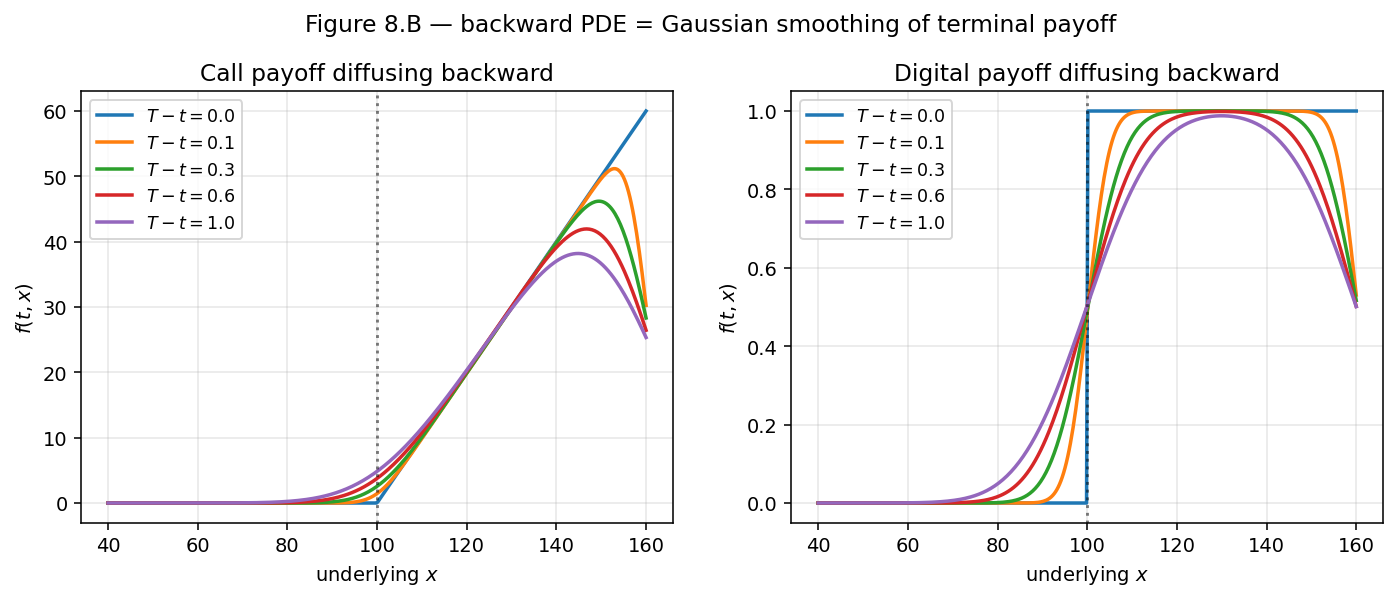
\includegraphics[keepaspectratio]{figures/ch04-heat-analogy.png}}
\emph{As \(t\) moves backward from \(T\) toward \(0\), the terminal
payoff \(\varphi\) diffuses and smooths: kinks (vanilla calls) round
off, step functions (digitals) bloom into Gaussian-shaped bumps. Every
option price is literally a smoothed payoff, where the smoothing kernel
is a Gaussian of width \(\sqrt{T-t}\).}

\begin{figure}
\centering
\pandocbounded{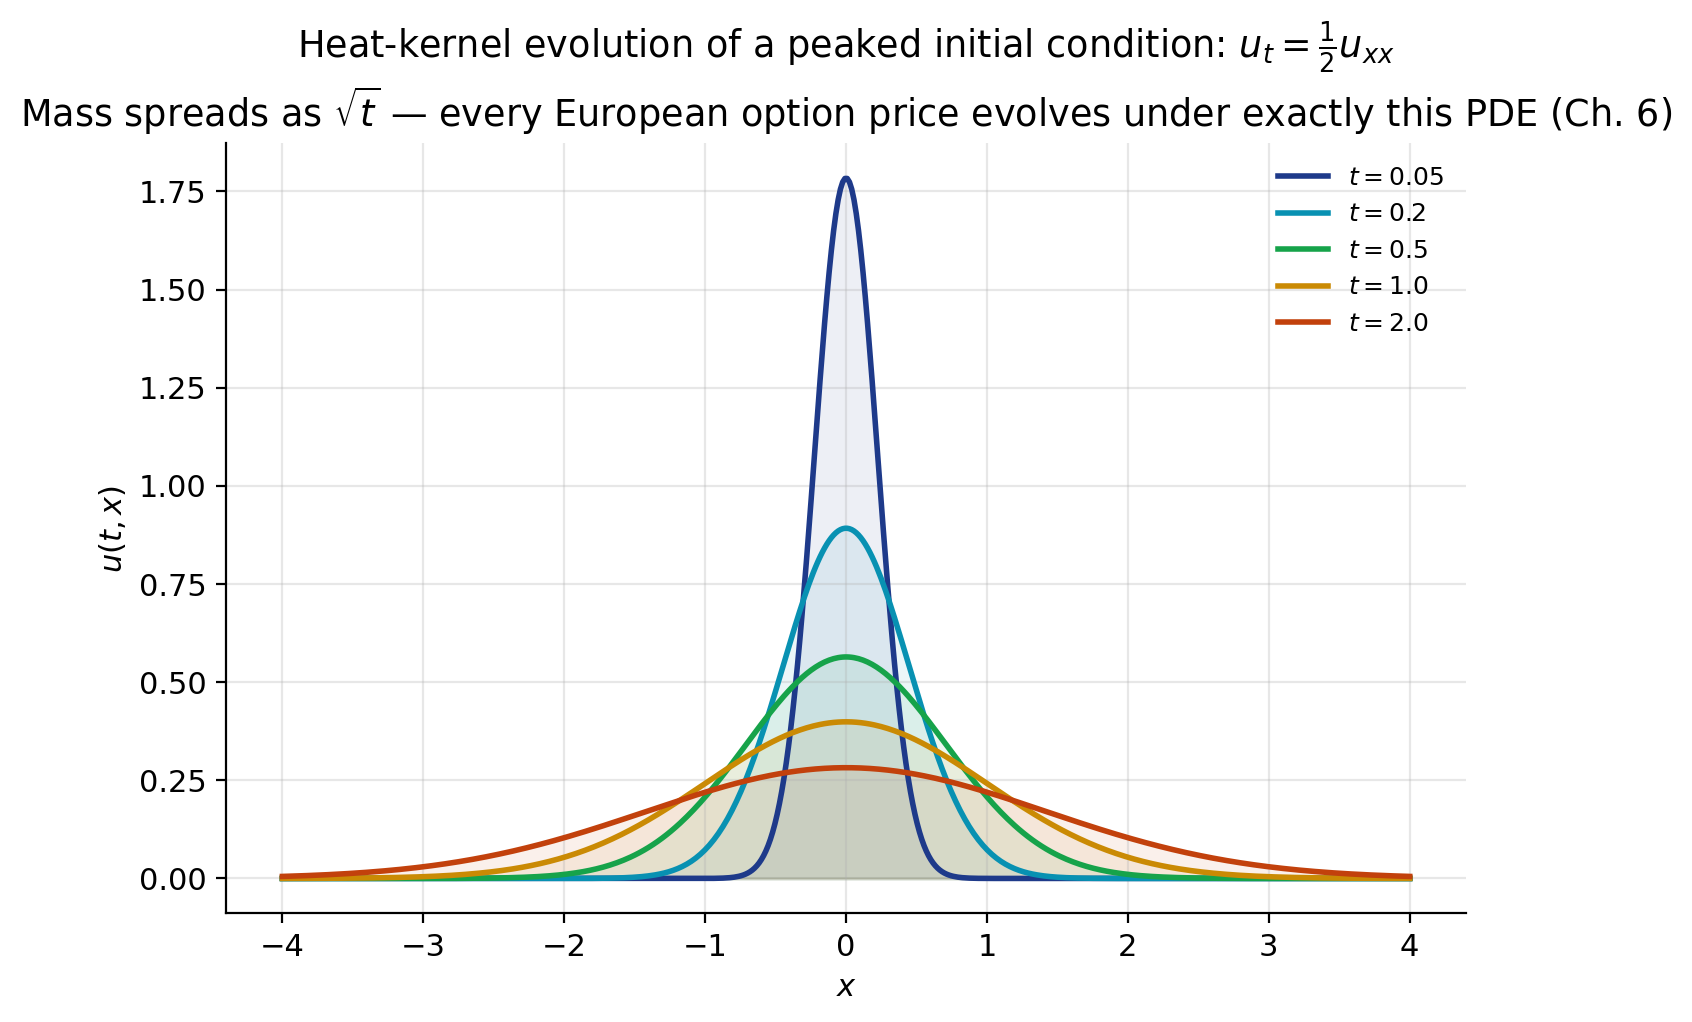
\includegraphics[keepaspectratio]{figures/ch04-heat-kernel.png}}
\caption{Heat-kernel evolution of a peaked initial profile under
\(u_t = \tfrac{1}{2} u_{xx}\) at \(t = 0.05, 0.2, 0.5, 1.0, 2.0\). Mass
spreads as \(\sqrt{t}\) --- this \emph{is} the Black-Scholes price
evolution after the standard log-transform (Ch. 6), and is why a digital
option printed sharply at expiry diffuses into a smooth bump as we step
back in time}
\end{figure}

\subsection{4.2.2 What the expectation
is}\label{what-the-expectation-is}

The right-hand side of \((4.2)\) averages \(\varphi(X_T)\) over Brownian
trajectories starting at \((t, x)\). Because BM is Markov, the
expectation depends only on \((t, x)\), never on how we got to \(x\) ---
which is why \(f\) is a function of two real variables rather than a
functional on path space.

\subsection{4.2.3 Path-integral intuition --- why the equivalence is not
magic}\label{path-integral-intuition-why-the-equivalence-is-not-magic}

Markov plus local dynamics force \((4.1)\). The scoreboard obeys the
tower identity

\[
f(t, x) \;=\; \mathbb{E}\!\left[\,f(t + \mathrm{d}t, \, x + \mathrm{d}W)\,\right].
\tag{4.3}
\]

Taylor-expand the right-hand side, use \(\mathbb{E}[\mathrm{d}W] = 0\)
and the Itô shorthand \((\mathrm{d}W)^2 = \mathrm{d}t\), divide by
\(\mathrm{d}t\), and the residual
\(0 = \partial_t f + \tfrac12 \partial_{xx} f\) is the PDE. The terminal
condition is automatic: at \(t = T\) the scoreboard reads the payoff
directly. The next section turns this sketch into a proof.

\begin{center}\rule{0.5\linewidth}{0.5pt}\end{center}

\section{4.3 A Martingale Derivation of the Backward
PDE}\label{a-martingale-derivation-of-the-backward-pde}

The clean derivation: \(f(s, X_s)\) is a martingale by the tower
property, Itô applied to a martingale forces the drift to vanish, and
that vanishing drift is the PDE. This three-move template --- (i) write
the price as a conditional expectation, (ii) apply Itô, (iii) kill the
drift --- is reused in every pricing PDE derivation in the guide.

\subsection{4.3.1 Setup and the
candidate}\label{setup-and-the-candidate}

Fix a horizon \(T\) and a payoff \(\varphi : \mathbb{R} \to \mathbb{R}\)
with polynomial growth. Let \(X_t\) be a standard Brownian motion.
Define the candidate pricing function

\[
f(t, x) \;\equiv\; \mathbb{E}\!\left[\,\varphi(X_T)\,\big|\,X_t = x\,\right] \;=\; \mathbb{E}_{t,x}[\varphi(X_T)].
\tag{4.4}
\]

The question the proof will answer is: \emph{what PDE does \(f\) satisfy
as a function of \((t, x)\)?} The answer is
\((\partial_t + \tfrac12 \partial_{xx})f = 0\) with terminal data
\(f(T, x) = \varphi(x)\), derivable from (a) iterated expectation and
(b) Itô's lemma applied to \(f(t, X_t)\).

\subsection{\texorpdfstring{4.3.2 The auxiliary process
\(\eta_s = f(s, X_s)\)}{4.3.2 The auxiliary process \textbackslash eta\_s = f(s, X\_s)}}\label{the-auxiliary-process-eta_s-fs-x_s}

Define a stochastic process indexed by the intermediate time
\(s \in [t, T]\):

\[
\eta_s \;\equiv\; f(s, X_s) \;=\; \mathbb{E}\!\left[\,\varphi(X_T)\,\big|\,X_s\,\right].
\tag{4.5}
\]

Geometrically, \(\eta_s\) is ``the best current guess of
\(\varphi(X_T)\) given everything known up to time \(s\).'' Because
\(X\) is Markov, conditioning on the full filtration \(\mathcal{F}_s\)
of the Brownian motion collapses to conditioning on the single random
variable \(X_s\):

\[
\mathbb{E}\!\left[\varphi(X_T) \,\big|\, \mathcal{F}_s\right] \;=\; \mathbb{E}\!\left[\varphi(X_T) \,\big|\, X_s\right] \;=\; f(s, X_s) \;=\; \eta_s.
\tag{4.6}
\]

The first equality is the Markov property of Brownian motion
(independent increments collapse the filtration dependence to the
current state); the second is the definition of \(f\); the third is
notation. This three-step unwinding is worth memorising because it
reappears in every measure-change, numeraire-swap, and forward-measure
derivation in later chapters.

\subsection{\texorpdfstring{4.3.3 Tower law \(\Rightarrow\) \(\eta\) is
a
martingale}{4.3.3 Tower law \textbackslash Rightarrow \textbackslash eta is a martingale}}\label{tower-law-rightarrow-eta-is-a-martingale}

Claim. The process \(s \mapsto \eta_s\) is a martingale in \(s\) under
the natural filtration \(\{\mathcal{F}_s\}\) of \(X\). Concretely, for
any \(t \le s_1 \le s_2 \le T\),

\[
\mathbb{E}\!\left[\eta_{s_2} \,\big|\, \mathcal{F}_{s_1}\right] \;=\; \eta_{s_1}.
\tag{4.7}
\]

\emph{Proof.} Plug in the definition:

\[
\mathbb{E}[\eta_{s_2} | \mathcal{F}_{s_1}] \;=\; \mathbb{E}\!\left[\,\mathbb{E}[\varphi(X_T) | \mathcal{F}_{s_2}]\,\big|\,\mathcal{F}_{s_1}\right].
\]

The outer expectation is over information up to \(s_1\); the inner
expectation is over information up to \(s_2 \ge s_1\). Apply the tower
property of conditional expectations ---
\(\mathbb{E}[\mathbb{E}[A | \mathcal{G}] | \mathcal{H}] = \mathbb{E}[A | \mathcal{H}]\)
whenever \(\mathcal{H} \subseteq \mathcal{G}\) --- with
\(\mathcal{H} = \mathcal{F}_{s_1}\) and
\(\mathcal{G} = \mathcal{F}_{s_2}\) (the latter is indeed finer because
more time has passed):

\[
\mathbb{E}\!\left[\,\mathbb{E}[\varphi(X_T) | \mathcal{F}_{s_2}]\,\big|\,\mathcal{F}_{s_1}\right] \;=\; \mathbb{E}[\varphi(X_T) | \mathcal{F}_{s_1}] \;=\; \eta_{s_1}.
\]

Therefore \(\eta_{s_1} = \mathbb{E}[\eta_{s_2} | \mathcal{F}_{s_1}]\),
the martingale property. \(\square\)

The argument uses only nesting of filtrations plus iterated expectation.
\emph{Any} process of the form ``conditional expectation of a fixed
\(\mathcal{F}_T\)-measurable random variable'' is a martingale (a
\emph{Doob martingale}). The payoff \(\varphi(X_T)\) is the ``closing''
random variable; \(\eta_s\) is the stream of running conditional
expectations.

\subsection{\texorpdfstring{4.3.4 Itô's lemma on
\(\eta_s = f(s, X_s)\)}{4.3.4 Itô's lemma on \textbackslash eta\_s = f(s, X\_s)}}\label{ituxf4s-lemma-on-eta_s-fs-x_s}

Having established that \(\eta_s\) is a martingale, we now apply Itô's
lemma to read off what PDE \(f\) must satisfy. Assume
\(f \in C^{1,2}([0,T) \times \mathbb{R})\) --- continuously
differentiable in \(t\) once, in \(x\) twice. This is an a-posteriori
regularity result for Feynman-Kac solutions with smooth enough payoffs,
and we take it for granted here. Apply Itô's lemma II from Chapter 3
with \(X_s = W_s\):

\[
\mathrm{d}\eta_s \;=\; \partial_t f(s, X_s)\,\mathrm{d}s \;+\; \partial_x f(s, X_s)\,\mathrm{d}X_s \;+\; \tfrac12\,\partial_{xx} f(s, X_s)\,(\mathrm{d}X_s)^2.
\tag{4.8}
\]

Using the Itô shorthand \((\mathrm{d}X_s)^2 = \mathrm{d}s\) and grouping
the \(\mathrm{d}s\) and \(\mathrm{d}X_s\) terms,

\[
\mathrm{d}\eta_s \;=\; \underbrace{\left[\,\partial_t f + \tfrac12\,\partial_{xx} f\,\right]}_{\text{drift}}\mathrm{d}s \;+\; \underbrace{\partial_x f}_{\text{diffusion}}\,\mathrm{d}X_s,
\tag{4.9}
\]

with both partial derivatives evaluated at \((s, X_s)\).

\subsection{4.3.5 Drift-killing identity}\label{drift-killing-identity}

The diffusion term \(\partial_x f\,\mathrm{d}X_s\) integrated against
\(\mathrm{d}W\) is a pure stochastic integral, hence a martingale by the
construction of the Itô integral in Chapter 3. So the difference between
\(\eta_s\) and the martingale \(\int \partial_x f\,\mathrm{d}X\) is the
deterministic drift term
\(\int[\partial_t f + \tfrac12 \partial_{xx} f]\,\mathrm{d}s\). But we
proved in §4.3.3 that \(\eta_s\) is already a martingale. Subtracting a
martingale from a martingale leaves a martingale, so the drift term
\(\int[\partial_t f + \tfrac12 \partial_{xx} f]\,\mathrm{d}s\) is itself
a martingale.

Now the key fact: this drift is a process of \emph{bounded variation}
(it is an ordinary Riemann integral in \(s\)), and the only continuous
martingale of finite variation is the zero process. (By the Doob-Meyer
decomposition, the finite-variation part of a continuous semimartingale
starts at zero and is uniquely identified by the drift; combining ``is a
martingale'' with ``finite-variation part starts at zero'' forces the
integrand to vanish identically.) Therefore the drift vanishes:

\[
\int_t^s\!\left[\partial_t f(u, X_u) + \tfrac12\partial_{xx}f(u, X_u)\right]\mathrm{d}u \;\equiv\; 0 \quad \text{for every } s \in [t, T].
\]

Because this holds for every path (including paths visiting every real
number at arbitrarily chosen times) and the integrand is continuous, the
integrand must vanish pointwise:

\[
\boxed{\;\partial_t f(t, x) + \tfrac12\,\partial_{xx} f(t, x) \;=\; 0\;} \qquad \text{for all } (t, x) \in [0, T) \times \mathbb{R}.
\tag{4.10}
\]

This is the Kolmogorov backward equation, and we have just derived it
from the martingale property of the Doob-closed process \(\eta\).
\(\square\)

\begin{center}\rule{0.5\linewidth}{0.5pt}\end{center}

\section{4.4 Boundary Condition and Summary of the Zero-Drift
Case}\label{boundary-condition-and-summary-of-the-zero-drift-case}

The derivation of §4.3 produced the PDE \((4.10)\) from the martingale
property of \(\eta\), but we still need to verify the terminal condition
\(f(T, x) = \varphi(x)\). That is immediate from the definition of
\(f\): at \(s = T\) the conditioning has frozen the Brownian motion at
its terminal value, so

\[
\eta_T \;=\; \mathbb{E}[\varphi(X_T) | X_T] \;=\; \varphi(X_T),
\]

and evaluating at \(X_T = x\) gives \(f(T, x) = \varphi(x)\). The
boundary data is \emph{built into} the probabilistic construction.

\subsection{4.4.1 What the zero-drift theorem
says}\label{what-the-zero-drift-theorem-says}

Putting the pieces of §§4.2--4.3 together:

\begin{quote}
\textbf{Zero-drift Feynman-Kac.} Let \(X\) be a standard Brownian motion
and let \(\varphi : \mathbb{R} \to \mathbb{R}\) have polynomial growth.
The function \(f(t, x) = \mathbb{E}_{t, x}[\varphi(X_T)]\) is the
(unique classical) solution of the backward heat equation
\(\partial_t f + \tfrac12 \partial_{xx} f = 0\) on
\([0, T) \times \mathbb{R}\) with terminal data
\(f(T, \cdot) = \varphi(\cdot)\).
\end{quote}

The three ingredients of the proof --- Markov collapse, Doob-martingale
of expectations, drift-kill via Itô --- will \emph{all} reappear in
every subsequent generalisation. The only thing that changes is what one
drops into the Itô decomposition.

\subsection{4.4.2 A remark on regularity}\label{a-remark-on-regularity}

The derivation of §4.3 assumed \(f \in C^{1,2}\). For discontinuous
payoffs (digitals, indicators) standard practice is either to
approximate by smooth \(\varphi_n \to \varphi\) (Gaussian-kernel
smoothing handles the limit) or to invoke viscosity solutions. The
\(C^{1,2}\) hypothesis is convenient but not essential.

\begin{center}\rule{0.5\linewidth}{0.5pt}\end{center}

\section{\texorpdfstring{4.5 Example 1 --- Linear Payoff
\(\varphi(x) = x\)}{4.5 Example 1 --- Linear Payoff \textbackslash varphi(x) = x}}\label{example-1-linear-payoff-varphix-x}

A baseline sanity check. Consider the Cauchy problem

\[
\begin{cases}
\partial_t f + \tfrac12 \partial_{xx} f \;=\; 0, \\
f(T, x) \;=\; x.
\end{cases}
\tag{4.12}
\]

By Feynman-Kac \((4.2)\),

\[
f(t, x) \;=\; \mathbb{E}_{t, x}[X_T],
\]

where \(X\) is a standard Brownian motion. Brownian increments are
Gaussian,

\[
X_T - X_t \;\sim\; \mathcal{N}(0, T - t), \qquad \text{so} \qquad X_T \stackrel{d}{=} x + \sqrt{T - t}\,Z, \quad Z \sim \mathcal{N}(0, 1).
\]

Therefore

\[
f(t, x) \;=\; \mathbb{E}_{t, x}\!\left[\,x + \sqrt{T - t}\,Z\,\right] \;=\; x \;+\; \sqrt{T - t}\cdot\mathbb{E}[Z] \;=\; x.
\tag{4.13}
\]

\textbf{PDE verification.} With \(f(t, x) = x\), \(\partial_t f = 0\),
\(\partial_x f = 1\), \(\partial_{xx} f = 0\), so
\(\partial_t f + \tfrac12 \partial_{xx} f = 0\). Terminal condition
\(f(T, x) = x\) holds by inspection. Both branches agree.

\subsection{4.5.1 Why this answer is
natural}\label{why-this-answer-is-natural}

Linear payoffs have zero convexity; Jensen is equality and the
expectation equals the initial state. A linear payoff is a forward on a
driftless underlying --- no convexity premium. As soon as the payoff
bends, the Itô correction bites.

\begin{center}\rule{0.5\linewidth}{0.5pt}\end{center}

\section{\texorpdfstring{4.6 Example 2 --- Quadratic Payoff
\(\varphi(x) = x^2\)}{4.6 Example 2 --- Quadratic Payoff \textbackslash varphi(x) = x\^{}2}}\label{example-2-quadratic-payoff-varphix-x2}

The first nontrivial case --- and the simplest variance-swap-style
replication. Solve

\[
\begin{cases}
\partial_t f + \tfrac12 \partial_{xx} f \;=\; 0, \\
f(T, x) \;=\; x^2.
\end{cases}
\tag{4.14}
\]

Feynman-Kac gives

\[
f(t, x) \;=\; \mathbb{E}_{t, x}[X_T^2] \;=\; \mathbb{E}_{t, x}\!\left[\,\big((X_T - X_t) + X_t\big)^2\,\right],
\]

with \(X_T - X_t \sim \mathcal{N}(0, T - t)\) and \(X_t = x\) under
\(\mathbb{E}_{t, x}\). Expanding the square and taking expectations term
by term:

\[
f(t, x) \;=\; \mathbb{E}_{t, x}\!\left[\,(X_T - X_t)^2 + 2 X_t (X_T - X_t) + X_t^2\,\right] \;=\; (T - t) \;+\; 0 \;+\; x^2,
\]

where the three contributions come from
\(\mathbb{E}[(X_T - X_t)^2] = \mathrm{Var}(X_T - X_t) = T - t\),
\(\mathbb{E}[(X_T - X_t)] = 0\), and
\(\mathbb{E}[X_t^2 | X_t = x] = x^2\). Hence

\[
\boxed{\;f(t, x) \;=\; x^2 + (T - t)\;}.
\tag{4.15}
\]

\textbf{PDE verification.} With \(f(t, x) = x^2 + (T - t)\),
\(\partial_t f = -1\), \(\partial_{xx} f = 2\), so
\(\partial_t f + \tfrac12 \partial_{xx} f = -1 + 1 = 0\). At \(t = T\):
\(f(T, x) = x^2 + 0 = x^2\). Both the PDE and the terminal condition are
satisfied.

\subsection{4.6.1 Convexity reading and variance-swap
interpretation}\label{convexity-reading-and-variance-swap-interpretation}

The extra \((T - t)\) in \((4.15)\) is the \emph{time-value of
convexity}: a convex payoff rewards variance, and Brownian increments
supply exactly \(\mathrm{Var}(X_T | X_t = x) = T - t\). Equivalently,
Itô's lemma applied to \(F(x) = x^2\) gives
\(X_T^2 = X_t^2 + 2\!\int_t^T X_s\,\mathrm{d}X_s + (T - t)\); the middle
martingale term vanishes under expectation and recovers \((4.15)\). The
same identity prices a variance swap with strike \(x^2\) in the
driftless, no-discount setting: the fair forward value is
\(x^2 + (T - t)\).

\pandocbounded{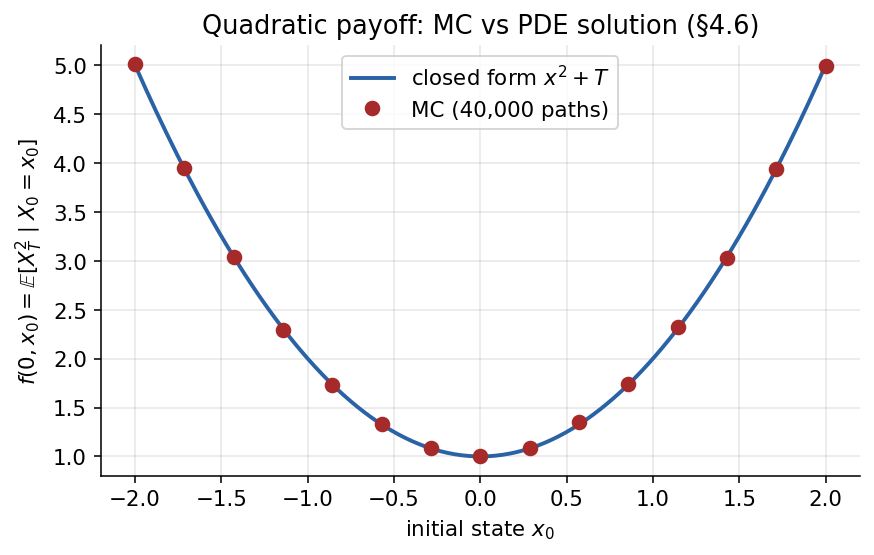
\includegraphics[keepaspectratio]{figures/ch04-quadratic-mc-vs-pde.png}}
\emph{Sanity check of \((4.15)\): Monte-Carlo averages of \(X_T^2\) at a
grid of initial states \(x_0\) (red dots) fall exactly on the PDE closed
form \(x_0^2 + T\) (blue curve). The \(+T\) offset is the ``time-value
of variance'' --- the convexity premium that Brownian motion pays out
for a quadratic payoff.}

\begin{center}\rule{0.5\linewidth}{0.5pt}\end{center}

\section{\texorpdfstring{4.7 Example 3 --- Exponential Payoffs
\(\varphi(x) = e^{ax}\)}{4.7 Example 3 --- Exponential Payoffs \textbackslash varphi(x) = e\^{}\{ax\}}}\label{example-3-exponential-payoffs-varphix-eax}

The log-space analogue of every log-normal pricing problem in the guide:
substitute \(X = \ln S\) and the answer feeds into Black--Scholes,
Black-76, and most rate/credit closed forms.

\subsection{\texorpdfstring{4.7.1 Base case
\(\varphi(x) = e^{-x}\)}{4.7.1 Base case \textbackslash varphi(x) = e\^{}\{-x\}}}\label{base-case-varphix-e-x}

Solve

\[
\begin{cases}
\partial_t f + \tfrac12 \partial_{xx} f \;=\; 0, \\
f(T, x) \;=\; e^{-x}.
\end{cases}
\tag{4.16}
\]

Feynman-Kac gives

\[
f(t, x) \;=\; \mathbb{E}_{t, x}[\,e^{-X_T}\,].
\]

Because \(X_T | X_t = x\) is \(\mathcal{N}(x, T - t)\), apply the
Gaussian moment-generating function
\(\mathbb{E}[e^{\lambda Y}] = e^{\lambda \mu + \tfrac12 \lambda^2 \sigma^2}\)
with \(\lambda = -1\), \(\mu = x\), \(\sigma^2 = T - t\):

\[
\boxed{\;f(t, x) \;=\; e^{-x + \tfrac12 (T - t)}\;}.
\tag{4.17}
\]

\textbf{PDE verification.} With \(f = e^{-x + \tfrac12(T - t)}\):
\(\partial_t f = -\tfrac12 f\), \(\partial_x f = -f\),
\(\partial_{xx} f = f\). Then
\(\partial_t f + \tfrac12 \partial_{xx} f = -\tfrac12 f + \tfrac12 f = 0\).
Terminal condition \(f(T, x) = e^{-x}\) holds.

\textbf{Jensen bump.} Notice
\(f(t, x) = e^{-x} \cdot e^{\tfrac12 (T - t)}\) --- the answer exceeds
the payoff evaluated at the mean \(e^{-x}\) by the factor
\(e^{\tfrac12(T - t)}\). This is the \emph{convexity premium}. In the
log variable this is exactly the \(\tfrac12 \sigma^2 t\) Itô correction
that will reappear in the Black-Scholes formula. Its sign follows from
Jensen's inequality applied to the convex function \(e^{-x}\):
\(\mathbb{E}[e^{-X_T}] \ge e^{-\mathbb{E}[X_T]} = e^{-x}\), with strict
inequality whenever \(X_T\) has nonzero variance.

\subsection{\texorpdfstring{4.7.2 General exponent
\(\varphi(x) = e^{ax}\)}{4.7.2 General exponent \textbackslash varphi(x) = e\^{}\{ax\}}}\label{general-exponent-varphix-eax}

A one-parameter generalisation that shows the convexity bump scales as
\(a^2\), not \(|a|\). Solve

\[
\begin{cases}
\partial_t f + \tfrac12 \partial_{xx} f \;=\; 0, \\
f(T, x) \;=\; e^{ax},
\end{cases} \qquad a \in \mathbb{R}.
\tag{4.18}
\]

By Feynman-Kac, using \(X_T = x + (X_T - X_t)\) with
\(X_T - X_t \sim \mathcal{N}(0, T - t)\),

\[
f(t, x) \;=\; \mathbb{E}_{t, x}[\,e^{a X_T}\,] \;=\; e^{ax}\cdot \mathbb{E}[\,e^{a (X_T - X_t)}\,] \;=\; e^{ax}\cdot e^{\tfrac12 a^2 (T - t)},
\]

using the Gaussian MGF with \(\lambda = a\), \(\sigma^2 = T - t\).
Compactly,

\[
\boxed{\;f(t, x) \;=\; \exp\!\left\{\,a\,x \;+\; \tfrac12\,a^2\,(T - t)\,\right\}\;}.
\tag{4.19}
\]

\textbf{PDE verification.} Let \(\gamma = \tfrac12 a^2\). Then
\(f = e^{ax + \gamma(T - t)}\) gives \(\partial_t f = -\gamma f\),
\(\partial_x f = a f\), \(\partial_{xx} f = a^2 f\). Plugging into the
PDE:

\[
\partial_t f + \tfrac12 \partial_{xx} f \;=\; -\gamma f + \tfrac12 a^2 f \;=\; -\tfrac12 a^2 f + \tfrac12 a^2 f \;=\; 0. \quad\checkmark
\]

Terminal: \(f(T, x) = e^{ax + 0} = e^{ax}\).

\pandocbounded{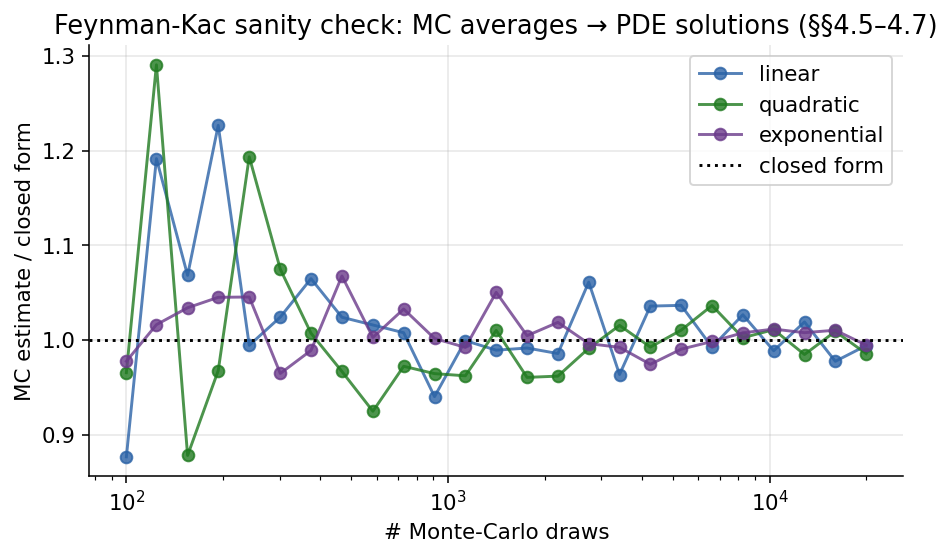
\includegraphics[keepaspectratio]{figures/ch04-fk-mc-check.png}}
\emph{For each of the three worked payoffs (linear \(x\), quadratic
\(x^2\), exponential \(e^{ax}\) with \(a=0.8\)), Monte-Carlo averaging
over \(N\) Brownian endpoints \(X_T \sim \mathcal{N}(x_0, T)\) converges
at rate \(1/\sqrt{N}\) to the Gaussian-MGF closed form from
\((4.13)\)--\((4.19)\).}

\begin{figure}
\centering
\pandocbounded{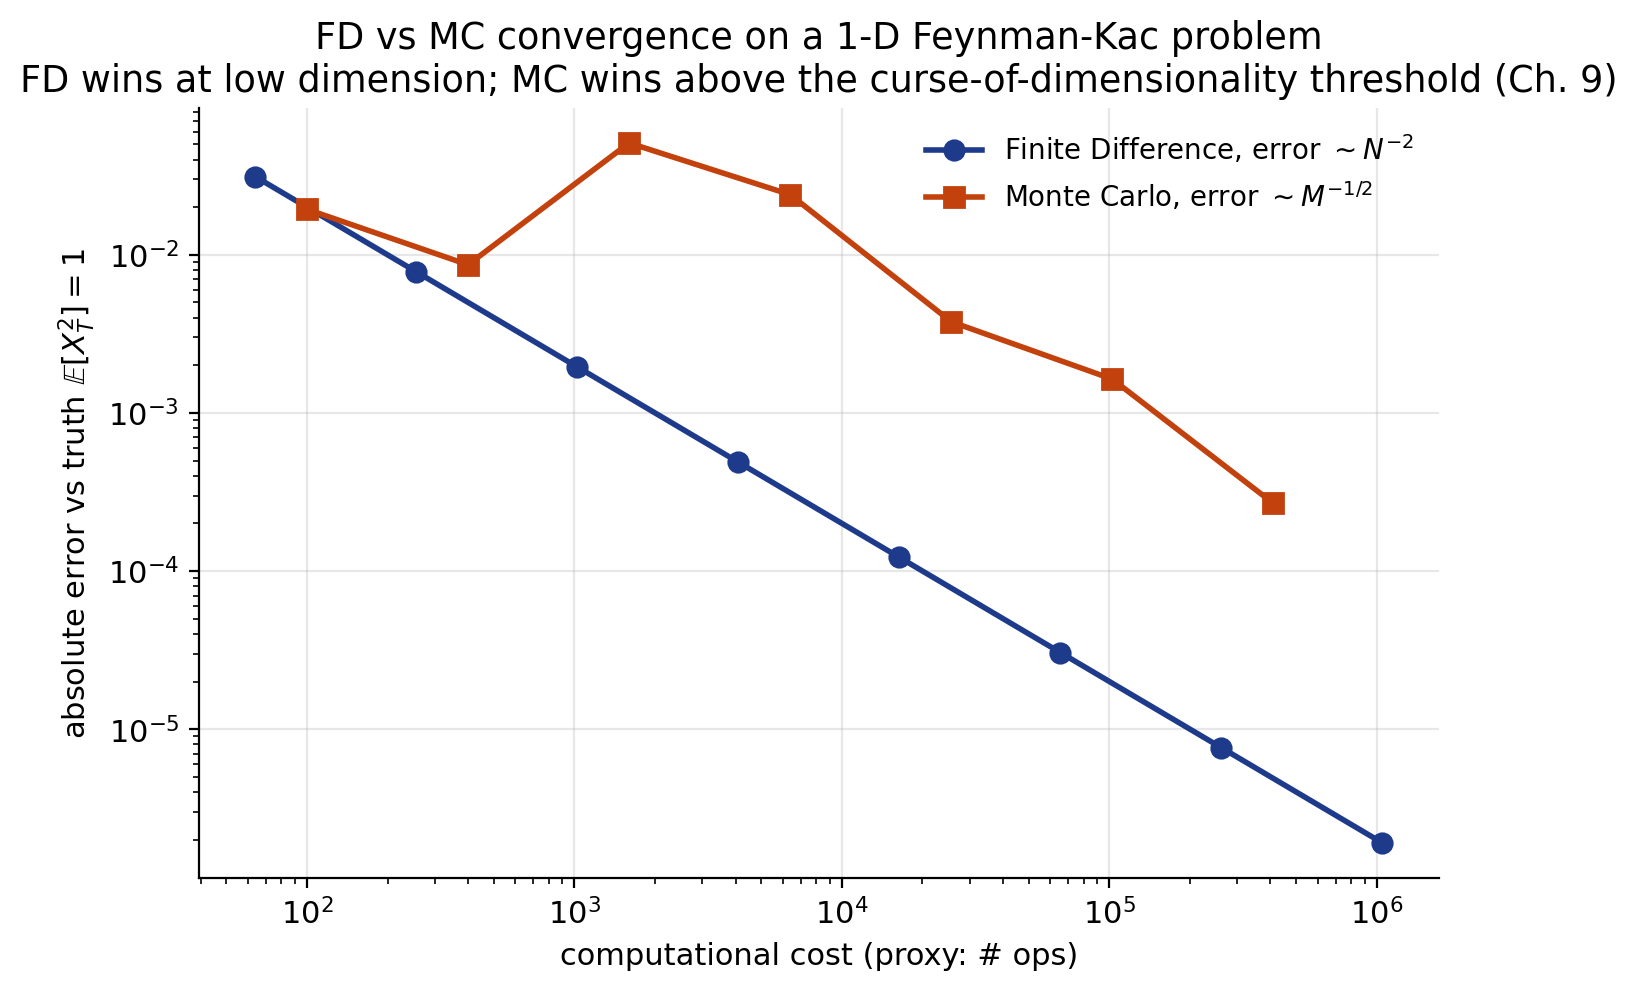
\includegraphics[keepaspectratio]{figures/ch04-fd-vs-mc.png}}
\caption{FD vs MC error convergence on a 1-D Feynman-Kac benchmark
(\(\mathbb{E}[X_T^2]\)): finite-difference error decays as \(N^{-2}\),
MC as \(M^{-1/2}\). FD dominates in 1-3D; MC's dimension-free constant
wins for high-dimensional baskets (the curse-of-dimensionality cliff
sits around \(d=5\))}
\end{figure}

\begin{center}\rule{0.5\linewidth}{0.5pt}\end{center}

\section{4.8 Feynman-Kac with Drift, Diffusion, and
Discounting}\label{feynman-kac-with-drift-diffusion-and-discounting}

Real pricing needs three extensions: a nonzero drift, an arbitrary
diffusion coefficient, and a discount on the payoff. We add all three at
once.

\subsection{4.8.1 Statement}\label{statement}

Let \(a \in \mathbb{R}\), \(b > 0\), and \(c \in \mathbb{R}\) be
constants. Consider the backward Cauchy problem with a lower-order term:

\[
\begin{cases}
\partial_t f(t, x) \;+\; a\,\partial_x f(t, x) \;+\; \tfrac12\,b^2\,\partial_{xx} f(t, x) \;=\; c\,f(t, x), \\[2pt]
f(T, x) \;=\; \varphi(x).
\end{cases}
\tag{4.20}
\]

The probabilistic representation of the solution is

\[
\boxed{\;f(t, x) \;=\; \mathbb{E}_{t, x}\!\left[\,e^{-c(T - t)}\,\varphi(X_T)\,\right],\;}
\tag{4.21}
\]

where \(X = (X_s)_{s \ge 0}\) is a drifted Brownian motion solving

\[
\mathrm{d}X_s \;=\; a\,\mathrm{d}s \;+\; b\,\mathrm{d}W_s, \qquad W \text{ a standard BM},
\tag{4.22}
\]

i.e.~\(X_s = X_0 + a\,s + b\,W_s\) (arithmetic Brownian motion with
drift \(a\) and volatility \(b\)).

\begin{figure}
\centering
\pandocbounded{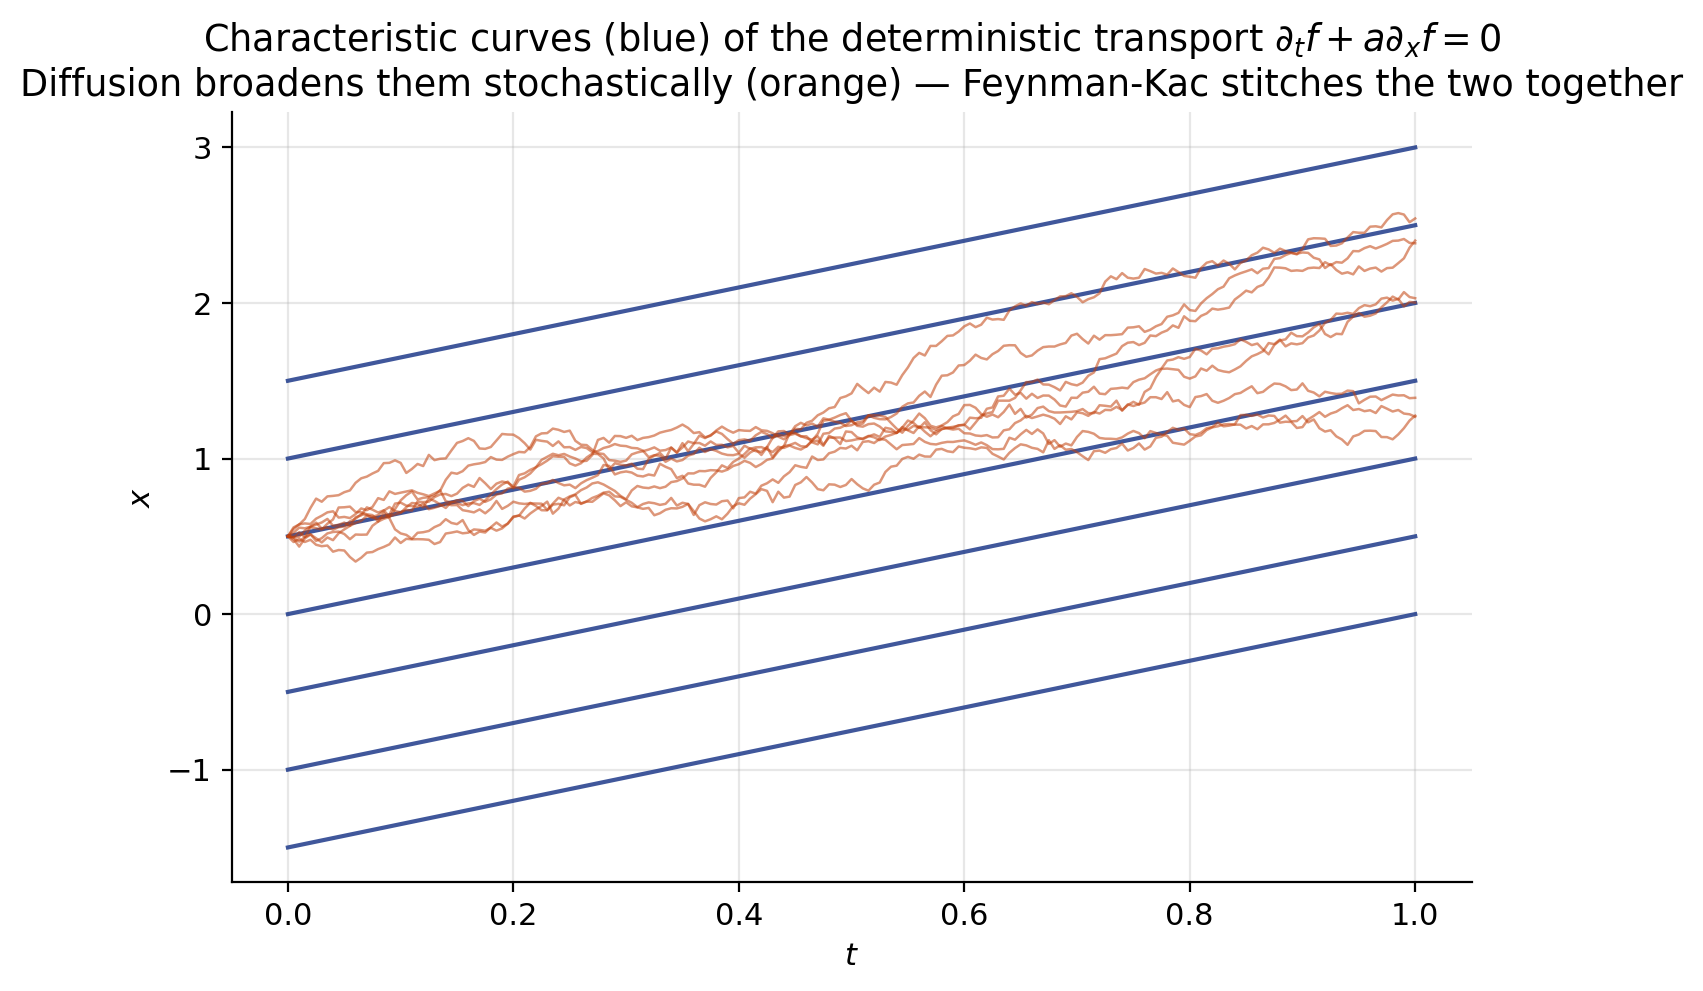
\includegraphics[keepaspectratio]{figures/ch04-characteristics.png}}
\caption{Characteristic curves \(x = x_0 + at\) of the pure-transport
operator \(\partial_t f + a\partial_x f = 0\) (blue) and sample paths of
the full SDE with diffusion (orange) around one of them. Feynman-Kac
sews the deterministic transport to the stochastic spread --- the same
factorisation that decomposes a corporate-bond return into ``forward
roll-down'' plus ``credit shock''}
\end{figure}

\subsection{4.8.2 Proof sketch}\label{proof-sketch}

Start from the expectation
\(f(t, x) = \mathbb{E}_{t, x}[e^{-c(T - t)}\varphi(X_T)]\) and apply
Itô's lemma to the auxiliary process

\[
g_s \;\equiv\; e^{-c(s - t)}\,f(s, X_s), \qquad s \in [t, T].
\]

Compute \(\mathrm{d}g_s\) using the product rule plus Itô's lemma III
applied to \(f(s, X_s)\):

\[
\mathrm{d}g_s \;=\; e^{-c(s - t)}\!\left\{-c\,f\,\mathrm{d}s \;+\; \left[\partial_t f + a\,\partial_x f + \tfrac12 b^2 \partial_{xx} f\right]\mathrm{d}s \;+\; b\,\partial_x f\,\mathrm{d}W_s\right\}.
\tag{4.23}
\]

For \(g_s\) to be a martingale --- which it must be, because
\(g_T = e^{-c(T - t)}\varphi(X_T)\) and conditional expectations of
fixed random variables are martingales --- the \(\mathrm{d}s\) drift
must vanish:

\[
-c\,f + \partial_t f + a\,\partial_x f + \tfrac12 b^2 \partial_{xx} f \;=\; 0,
\]

which is exactly the PDE \((4.20)\). Conversely, if \(f\) satisfies the
PDE, the drift of \(g_s\) is identically zero; \(g_s\) is therefore a
martingale, and taking \(\mathbb{E}_{t, x}\) of \(g_t = f(t, x)\) and
\(g_T = e^{-c(T - t)}\varphi(X_T)\) yields the representation
\((4.21)\).

The two-way proof is the essence of Feynman-Kac: the PDE \emph{is} the
drift-killing condition for \(e^{-c(s - t)} f(s, X_s)\), and any
function satisfying that PDE automatically represents an expectation.

\subsection{4.8.3 Role of each
coefficient}\label{role-of-each-coefficient}

Each term in \((4.20)\) has a direct counterpart in \((4.21)\):

{\def\LTcaptype{none} % do not increment counter
\begin{longtable}[]{@{}
  >{\raggedright\arraybackslash}p{(\linewidth - 2\tabcolsep) * \real{0.5000}}
  >{\raggedright\arraybackslash}p{(\linewidth - 2\tabcolsep) * \real{0.5000}}@{}}
\toprule\noalign{}
\begin{minipage}[b]{\linewidth}\raggedright
PDE term
\end{minipage} & \begin{minipage}[b]{\linewidth}\raggedright
SDE / expectation counterpart
\end{minipage} \\
\midrule\noalign{}
\endhead
\bottomrule\noalign{}
\endlastfoot
\(a\,\partial_x f\) & drift of \(X\): each path is pushed by
\(a\,\mathrm{d}s\) per step. \\
\(\tfrac12 b^2\,\partial_{xx} f\) & diffusion of \(X\): paths spread
with variance \(b^2\,\mathrm{d}s\) per step. \\
\(-c\,f\) & exponential decay / discount factor \(e^{-c(T - t)}\)
applied to the payoff. \\
terminal \(f(T, x) = \varphi(x)\) & the expectation at \(s = T\) is
literally \(\varphi(X_T)\) with \(X_T = x\). \\
\end{longtable}
}

The dictionary reading of \((4.20) \Leftrightarrow (4.21)\):
\emph{``\(a\) and \(b\) pick the law of \(X\); \(c\) attaches a
per-unit-time discount to every path.''}

\subsection{4.8.4 Worked case: exponential payoff with drift, diffusion,
and
discount}\label{worked-case-exponential-payoff-with-drift-diffusion-and-discount}

Solve \((4.20)\) with \(\varphi(x) = e^{-x}\):

\[
\begin{cases}
\partial_t f + a\,\partial_x f + \tfrac12 b^2 \partial_{xx} f \;=\; c\,f, \\
f(T, x) \;=\; e^{-x}.
\end{cases}
\tag{4.24}
\]

By \((4.21)\),

\[
f(t, x) \;=\; \mathbb{E}_{t, x}\!\left[\,e^{-X_T}\,e^{-c(T - t)}\,\right].
\]

The increment of \(X\) under the drifted BM \((4.22)\) is

\[
X_T - X_t \;=\; a(T - t) + b\,(W_T - W_t) \;\stackrel{d}{=}\; a(T - t) + b\sqrt{T - t}\,Z, \qquad Z \sim \mathcal{N}(0, 1),
\]

so \(X_T | X_t = x\) is Gaussian with mean \(x + a(T - t)\) and variance
\(b^2 (T - t)\). Substituting,

\[
f(t, x) \;=\; \mathbb{E}\!\left[\,\exp\!\left\{-x - a(T - t) - b\sqrt{T - t}\,Z - c(T - t)\right\}\,\right].
\]

Taking the Gaussian MGF of \(-b\sqrt{T - t}\,Z\), which contributes
\(e^{\tfrac12 b^2 (T - t)}\):

\[
f(t, x) \;=\; \exp\!\left\{-x - a(T - t) + \tfrac12 b^2 (T - t) - c(T - t)\right\}.
\]

Collecting terms with common factor \((T - t)\):

\[
\boxed{\;f(t, x) \;=\; \exp\!\left\{\,-x \;-\; \left(a + c - \tfrac12 b^2\right)(T - t)\,\right\}\;}.
\tag{4.25}
\]

Equivalently, defining \(\gamma = a + c - \tfrac12 b^2\) for shorthand,

\[
f(t, x) \;=\; e^{-x - \gamma(T - t)}.
\tag{4.26}
\]

\subsection{\texorpdfstring{4.8.5 Reading formula \((4.25)\) as a
ledger}{4.8.5 Reading formula (4.25) as a ledger}}\label{reading-formula-4.25-as-a-ledger}

The exponent \(-x - (a + c - \tfrac12 b^2)(T - t)\) has four
contributions: \(-x\) from the payoff base, \(-a(T - t)\) from drift,
\(+\tfrac12 b^2 (T - t)\) from Jensen/convexity, and \(-c(T - t)\) from
discount. Sanity limits: \(a = c = 0\), \(b = 1\) recovers \((4.17)\);
\(b = 0\) recovers pure deterministic evolution with no convexity. A
direct PDE check with \(\gamma = a + c - \tfrac12 b^2\) and
\(f = e^{-x - \gamma(T - t)}\) gives \(\partial_t f = +\gamma f\),
\(\partial_x f = -f\), \(\partial_{xx} f = f\), and the LHS of
\((4.20)\) collapses to \((\gamma - a + \tfrac12 b^2 - c)f = 0\).

\begin{center}\rule{0.5\linewidth}{0.5pt}\end{center}

\section{4.9 Feynman-Kac with State- and Time-Dependent
Coefficients}\label{feynman-kac-with-state--and-time-dependent-coefficients}

Black--Scholes (equity), short-rate models (rates), and most other
workhorses need state-dependent \(a, b, c\) as functions of \((t, x)\).
We state and prove the general theorem, then read off three
instantiations.

\subsection{4.9.1 The general theorem}\label{the-general-theorem}

Let \(a, b, c : [0, T] \times \mathbb{R} \to \mathbb{R}\) be
sufficiently regular functions --- continuous with mild growth
conditions on \(a\) and \(b\), and boundedness on \(c\); these are the
conditions under which the associated SDE has a unique strong solution
and the corresponding PDE has a classical solution. Consider the Cauchy
problem

\[
\begin{cases}
\partial_t h(t, x) \;+\; a(t, x)\,\partial_x h(t, x) \;+\; \tfrac12\,b^2(t, x)\,\partial_{xx} h(t, x) \;=\; c(t, x)\,h(t, x), \\[2pt]
h(T, x) \;=\; H(x),
\end{cases}
\tag{4.34}
\]

with terminal payoff \(H : \mathbb{R} \to \mathbb{R}\) satisfying
polynomial growth. Then the solution admits the probabilistic
representation

\[
\boxed{\;h(t, x) \;=\; \mathbb{E}\!\left[\,\exp\!\left\{-\!\int_t^T c(u, X_u)\,\mathrm{d}u\right\}\,H(X_T)\,\Big|\,X_t = x\right],\;}
\tag{4.35}
\]

where the process \(X\) satisfies the Itô SDE

\[
\mathrm{d}X_s \;=\; a(s, X_s)\,\mathrm{d}s \;+\; b(s, X_s)\,\mathrm{d}W_s, \qquad s \in [t, T].
\tag{4.36}
\]

This is the \emph{complete} Feynman-Kac theorem used in practice. Every
linear parabolic pricing PDE in this guide is an instantiation of it,
and the dictionary between PDE coefficients and SDE/discount is strict.

\subsection{4.9.2 Three features worth
noting}\label{three-features-worth-noting}

\emph{The drift \(a(s, X_s)\) and diffusion \(b(s, X_s)\) may depend on
both time and the current state.} No constancy assumption is required.
The SDE \((4.36)\) is the general Itô diffusion, and Itô's lemma III
from Chapter 3 is exactly the tool we need.

\emph{The discount rate \(c(s, X_s)\) may itself be stochastic} --- a
function of the state \(X_s\). In this case the integrated discount
\(\int_t^T c(u, X_u)\,\mathrm{d}u\) is a path-dependent random variable,
not a deterministic number \(c(T - t)\). The path integral is exactly
how stochastic-rate bond pricing works: \(c(t, r) = r\) with \(X = r_t\)
a short-rate process yields bond prices
\(P(t, T) = \mathbb{E}_t[e^{-\int_t^T r_s\,\mathrm{d}s}]\).

\emph{The payoff \(H(X_T)\) is evaluated at the final state only.} We do
not allow path-dependent payoffs in the basic statement. Path-dependency
--- barrier options that knock out if the path touches a level, Asian
options that depend on the average price --- requires further machinery:
auxiliary state variables (e.g.~the running minimum becomes a second
state), augmented Itô processes, or variational inequalities for
American-style features. Each extension preserves the Feynman-Kac spirit
but with extra bookkeeping. The basic theorem \((4.34)\)--\((4.35)\)
covers every European-style payoff on a single state variable.

\subsection{4.9.3 Why the path-dependent discount is
necessary}\label{why-the-path-dependent-discount-is-necessary}

The PDE evaluates \(c(t, x)\) locally; the expectation accumulates
\(\int c(u, X_u)\,\mathrm{d}u\) along each path. For constant \(c\) the
path integral collapses to \(c(T - t)\) and we recover (4.21). For
\(c = x\) the PDE has a linear zero-order term; the expectation carries
\(e^{-\int X_u\,\mathrm{d}u}\) --- same content, different bookkeeping.

\subsection{4.9.4 Proof (integrating-factor
device)}\label{proof-integrating-factor-device}

Apply Itô to the discounted candidate

\[
Y_s \;\equiv\; \exp\!\left\{-\!\int_t^s c(u, X_u)\,\mathrm{d}u\right\}\cdot h(s, X_s), \qquad s \in [t, T].
\tag{4.37}
\]

The integrating factor \(e^{-\int_t^s c\,\mathrm du}\) has differential
\(-c(s, X_s)\,e^{-\int_t^s c\,\mathrm du}\,\mathrm ds\) (no
\(\mathrm dW\) piece, hence no covariation). Combining with Itô III on
\(h(s, X_s)\),

\[
\mathrm{d}Y_s \;=\; e^{-\int_t^s c\,\mathrm{d}u}\!\left\{\left[-c\,h + \partial_t h + a\,\partial_x h + \tfrac12 b^2\,\partial_{xx} h\right]\mathrm{d}s \;+\; b\,\partial_x h\,\mathrm{d}W_s\right\}.
\tag{4.38}
\]

The \(\mathrm{d}s\) coefficient vanishes by the PDE \((4.34)\), leaving
a pure stochastic integral. Under the standard integrability hypothesis
\(\mathbb{E}_{t,x}\!\int_t^T e^{-2\int_t^s c\,\mathrm du}\,b^2\,(\partial_x h)^2\,\mathrm ds < \infty\),
\(Y\) is a true martingale on \([t, T]\). Taking expectations of \(Y_t\)
and \(Y_T\) and using the terminal condition \(h(T, \cdot) = H(\cdot)\),

\[
h(t, x) \;=\; \mathbb{E}_{t, x}[Y_T] \;=\; \mathbb{E}_{t, x}\!\left[e^{-\int_t^T c\,\mathrm{d}u}\,H(X_T)\right]. \quad\square
\]

The integrating factor \(e^{-\int_t^s c\,\mathrm du}\) does the same job
as the time-\(0\)-discount move in §4.3.5: it converts what would be a
super-martingale candidate into a true martingale by absorbing the
spatial discount drift, and is the simplest instance of the
change-of-numeraire technique developed in Chapter 5. Two
specialisations to flag: \(c(t, x) = x\) with \(H = 1\) gives the
bond-price formula
\(P(t, x) = \mathbb{E}_{t, x}[e^{-\int_t^T X_u\,\mathrm du}]\) (Chapter
12); \(c(t, x) = r + \lambda(t, x)\) gives the survival-probability
building block of credit pricing.

\subsection{4.9.5 Reading off the Black-Scholes
PDE}\label{reading-off-the-black-scholes-pde}

Plug \(a(t, x) = r x\), \(b(t, x) = \sigma x\), \(c(t, x) = r\) into
\((4.34)\), all state-linear or constant. The PDE becomes

\[
\partial_t h + r x\,\partial_x h + \tfrac12 \sigma^2 x^2\,\partial_{xx} h \;=\; r\,h,
\tag{4.39}
\]

which is the Black-Scholes PDE. The expectation \((4.35)\) becomes

\[
h(t, x) \;=\; \mathbb{E}_{t, x}\!\left[e^{-r(T - t)}\,H(X_T)\right], \qquad \mathrm{d}X_s = r X_s\,\mathrm{d}s + \sigma X_s\,\mathrm{d}W_s,
\tag{4.40}
\]

which is the risk-neutral pricing formula for a claim \(H(X_T)\) on a
geometric-Brownian-motion underlying. The Black-Scholes formula for a
European call or put is therefore literally a corollary of the general
Feynman-Kac theorem; Chapter 6 derives it both this way and via the
independent hedging argument.

\subsection{4.9.6 Reading off the Vasicek bond
price}\label{reading-off-the-vasicek-bond-price}

Plug \(a(t, r) = \kappa(\theta - r)\), \(b(t, r) = \sigma\),
\(c(t, r) = r\), and \(H(r) = 1\) into \((4.34)\). The PDE becomes the
Vasicek bond-price PDE

\[
\partial_t P + \kappa(\theta - r)\,\partial_r P + \tfrac12 \sigma^2\,\partial_{rr} P \;=\; r\,P, \qquad P(T, r) = 1.
\tag{4.41}
\]

The expectation becomes

\[
P(t, r) \;=\; \mathbb{E}_{t, r}\!\left[e^{-\int_t^T r_s\,\mathrm{d}s}\right], \qquad \mathrm{d}r_s = \kappa(\theta - r_s)\,\mathrm{d}s + \sigma\,\mathrm{d}W_s,
\tag{4.42}
\]

the classical fair value of a zero-coupon bond under a Vasicek short
rate; Chapter 12 evaluates this expectation to obtain the affine closed
form \(P(t, r) = e^{A(t, T) - B(t, T) r}\).

\subsection{4.9.7 The unifying
observation}\label{the-unifying-observation}

Every linear PDE with a drift, a diffusion, and a discount term is a
Feynman--Kac PDE for some SDE and some discount rate. Identify the
coefficients, write the SDE, read off the expectation. Black--Scholes,
Vasicek, Hull--White, caplet, swaption, Heston --- all the same theorem
with different substitutions. The algebra of solving each is where the
later chapters spend their time.

\begin{center}\rule{0.5\linewidth}{0.5pt}\end{center}

\section{4.10 Case Study --- Vasicek Bond Pricing from the 2024 Treasury
Curve}\label{case-study-vasicek-bond-pricing-from-the-2024-treasury-curve}

\subsection{Case study: Vasicek calibrated to the 2024 US Treasury
curve}\label{case-study-vasicek-calibrated-to-the-2024-us-treasury-curve}

\textbf{Context.} In early 2024 the on-the-run US 10-year Treasury
traded near a 4.10\% yield, with the 2-year at 4.55\% and the 3-month
T-bill near 5.40\% --- a deeply inverted curve produced by the Fed's
hiking cycle (5.25\%--5.50\% policy rate) sitting above market
expectations of cuts later in the year. A Vasicek short rate
\(\mathrm{d}r_t = \kappa(\theta - r_t)\,\mathrm dt + \sigma\,\mathrm dW_t\)
fitted to that snapshot yields \(\kappa \approx 0.30\),
\(\theta \approx 0.035\), \(\sigma \approx 0.011\) (units:
years\(^{-1}\), percent, percent yr\(^{-1/2}\)) --- a slow
mean-reversion to a long-run rate well below the then-current 4.10\%
short rate.

\textbf{Math mapping.} This is \((4.42)\) in flight. The Vasicek bond
price \(P(t, r) = \mathbb{E}_{t, r}[e^{-\int_t^T r_s\,\mathrm ds}]\) is
the Feynman-Kac formula \((4.35)\) with
\(a(t, r) = \kappa(\theta - r)\), \(b(t, r) = \sigma\), \(c(t, r) = r\)
(the short rate itself is the discount), and terminal payoff \(H = 1\).
The affine ansatz \(P(t, r) = e^{A(t, T) - B(t, T)r}\) reduces the path
integral to two ODEs: \(B(t, T) = (1 - e^{-\kappa(T - t)})/\kappa\) and
\(A\) collecting the variance-of-integrated-rate term. With
\(T - t = 10\), \(B \approx 3.17\), and plugging \(r = 0.054\) gives
\(\ln P \approx A - 3.17 \cdot 0.054\); the convexity adjustment
\(\sigma^2 B^2(T-t)/(4\kappa)\) shaves about 0.6 bp off the implied
yield. The model recovers a 10-year zero yield of \(\approx 4.05\%\) ---
within 5 bp of the on-the-run quote, all of which is the
spline-vs-affine fitting residual on a curve with humps that a 1-factor
Vasicek cannot match. The bond price is \emph{literally} what falls out
of evaluating a Gaussian path integral over the integrated short rate.

\textbf{Lesson.} Feynman-Kac is not decorative. The bond desk does this
calibration every morning: take the observed short-rate path, fit
\((\kappa, \theta, \sigma)\) to a few benchmark maturities, and read off
every other point on the curve as a closed-form expectation \((4.42)\).
The mismatch in 2024 between the steeply inverted near end and a
single-factor Vasicek model is exactly the empirical motivation for the
multi-factor and time-dependent-\(\theta(t)\) extensions of Chapter 12
--- once \(\theta\) is allowed to vary, the Hull-White model fits the
entire 2024 curve to within 0.5 bp without changing the Feynman-Kac
structure of the pricing formula.

\begin{center}\rule{0.5\linewidth}{0.5pt}\end{center}

\section{4.11 Key Takeaways}\label{key-takeaways-3}

\begin{enumerate}
\def\labelenumi{\arabic{enumi}.}
\item
  \textbf{Two-way bridge.} A linear parabolic PDE with terminal data is
  \emph{equivalent} to a conditional expectation over an associated
  diffusion; the reader picks whichever side is easier for the problem
  at hand. Equations \((4.1)\)--\((4.2)\) for the base case,
  \((4.34)\)--\((4.35)\) in full generality.
\item
  \textbf{Proof template: three moves.} Every pricing PDE in the guide
  is derived by (i) writing the price as a conditional expectation, (ii)
  applying Itô to decompose its increment into drift plus martingale,
  (iii) demanding the drift vanish. Recurs in Chapters 6, 12, 15.
\item
  \textbf{Doob martingale + drift-kill.}
  \(\eta_s = \mathbb{E}[\varphi(X_T) | \mathcal{F}_s]\) is automatically
  a martingale by the tower property; a continuous martingale of bounded
  variation is identically zero, so its Itô drift must vanish --- and
  that vanishing drift \emph{is} the PDE.
\item
  \textbf{Three worked payoffs.} Linear \(\varphi(x) = x\): \(f = x\)
  (no convexity). Quadratic \(\varphi(x) = x^2\): \(f = x^2 + (T - t)\)
  (variance-swap identity). Exponential \(\varphi(x) = e^{ax}\):
  \(f = e^{ax + \tfrac12 a^2 (T - t)}\) (Jensen bump scales as \(a^2\)).
  Equations \((4.13)\), \((4.15)\), \((4.19)\).
\item
  \textbf{Constant-coefficient ledger.} For \(\varphi = e^{-x}\) with
  constant \(a, b, c\),
  \(f = \exp\{-x - (a + c - \tfrac12 b^2)(T - t)\}\) --- drift,
  discount, convexity each on its own line in the exponent. Equation
  \((4.25)\).
\item
  \textbf{General theorem.} For state-and-time-dependent \(a, b, c\),
  \(h(t, x) = \mathbb{E}_{t, x}[e^{-\int_t^T c(u, X_u)\,\mathrm du}\,H(X_T)]\)
  with
  \(\mathrm dX_s = a(s, X_s)\,\mathrm ds + b(s, X_s)\,\mathrm dW_s\).
  The integrating-factor device \((4.37)\)--\((4.38)\) proves it in one
  Itô calculation.
\item
  \textbf{Black-Scholes corollary.} \(a = rx\), \(b = \sigma x\),
  \(c = r\) recover the BS PDE and the GBM risk-neutral expectation. The
  closed-form call is the Gaussian integral evaluated; Chapter 6 fills
  in.
\item
  \textbf{Vasicek corollary.} \(a = \kappa(\theta - r)\),
  \(b = \sigma\), \(c = r\), \(H = 1\) recover the bond-price PDE;
  \(P(t, r) = \mathbb{E}_{t, r}[e^{-\int_t^T r_s\,\mathrm ds}]\) is
  affine in \(r\). The 2024 case study of §4.10 shows this recovering a
  Treasury yield to within 5 bp.
\item
  \textbf{PDE vs Monte-Carlo routing.} Low-dimensional smooth problems
  favour PDE; high-dimensional / path-dependent problems favour MC.
  Feynman-Kac guarantees the two answers agree, enabling
  cross-validation.
\item
  \textbf{Sign-convention reflex.} Discount appears as \(-c\,f\) on the
  PDE side and as \(e^{-c(T - t)}\) inside the expectation; mixing the
  conventions is the most common bookkeeping bug. Always anchor on the
  terminal condition first.
\end{enumerate}

\begin{center}\rule{0.5\linewidth}{0.5pt}\end{center}

\section{4.12 Reference Formulas}\label{reference-formulas-3}

\subsection{4.12.1 Feynman-Kac statements}\label{feynman-kac-statements}

{\def\LTcaptype{none} % do not increment counter
\begin{longtable}[]{@{}
  >{\raggedright\arraybackslash}p{(\linewidth - 4\tabcolsep) * \real{0.3333}}
  >{\raggedright\arraybackslash}p{(\linewidth - 4\tabcolsep) * \real{0.3333}}
  >{\raggedright\arraybackslash}p{(\linewidth - 4\tabcolsep) * \real{0.3333}}@{}}
\toprule\noalign{}
\begin{minipage}[b]{\linewidth}\raggedright
Object
\end{minipage} & \begin{minipage}[b]{\linewidth}\raggedright
Formula
\end{minipage} & \begin{minipage}[b]{\linewidth}\raggedright
Eq.
\end{minipage} \\
\midrule\noalign{}
\endhead
\bottomrule\noalign{}
\endlastfoot
F-K zero-drift PDE & \(\partial_t f + \tfrac12\,\partial_{xx} f = 0\),
\(f(T, x) = \varphi(x)\) & \((4.1)\) \\
F-K zero-drift expectation &
\(f(t, x) = \mathbb{E}_{t, x}[\varphi(X_T)]\), \(X\) a standard BM &
\((4.2)\) \\
F-K constant-coefficient PDE &
\(\partial_t f + a\,\partial_x f + \tfrac12 b^2\,\partial_{xx} f = c\,f\)
& \((4.20)\) \\
F-K constant-coefficient expectation &
\(f(t, x) = \mathbb{E}_{t, x}[e^{-c(T - t)}\varphi(X_T)]\),
\(\mathrm{d}X = a\,\mathrm{d}s + b\,\mathrm{d}W\) & \((4.21)\) \\
F-K general (state-dep. \(a, b, c\)) PDE &
\(\partial_t h + a(t, x)\,\partial_x h + \tfrac12 b^2(t, x)\,\partial_{xx} h = c(t, x)\,h\)
& \((4.34)\) \\
F-K general expectation &
\(h(t, x) = \mathbb{E}_{t, x}[e^{-\int_t^T c(u, X_u)\,\mathrm{d}u}\,H(X_T)]\)
& \((4.35)\) \\
SDE for the diffusion \(X\) &
\(\mathrm{d}X_s = a(s, X_s)\,\mathrm{d}s + b(s, X_s)\,\mathrm{d}W_s\) &
\((4.36)\) \\
\end{longtable}
}

\subsection{4.12.2 Derivation internals}\label{derivation-internals}

{\def\LTcaptype{none} % do not increment counter
\begin{longtable}[]{@{}
  >{\raggedright\arraybackslash}p{(\linewidth - 4\tabcolsep) * \real{0.3333}}
  >{\raggedright\arraybackslash}p{(\linewidth - 4\tabcolsep) * \real{0.3333}}
  >{\raggedright\arraybackslash}p{(\linewidth - 4\tabcolsep) * \real{0.3333}}@{}}
\toprule\noalign{}
\begin{minipage}[b]{\linewidth}\raggedright
Object
\end{minipage} & \begin{minipage}[b]{\linewidth}\raggedright
Formula
\end{minipage} & \begin{minipage}[b]{\linewidth}\raggedright
Eq.
\end{minipage} \\
\midrule\noalign{}
\endhead
\bottomrule\noalign{}
\endlastfoot
Local self-consistency (tower) &
\(f(t, x) = \mathbb{E}[f(t + \mathrm{d}t,\,x + \mathrm{d}W)]\) &
\((4.3)\) \\
Candidate pricing function &
\(f(t, x) = \mathbb{E}[\varphi(X_T) \mid X_t = x]\) & \((4.4)\) \\
Doob martingale &
\(\eta_s = f(s, X_s) = \mathbb{E}[\varphi(X_T) \mid X_s]\) &
\((4.5)\) \\
Markov collapse of filtration &
\(\mathbb{E}[\varphi(X_T) \mid \mathcal{F}_s] = \mathbb{E}[\varphi(X_T) \mid X_s]\)
& \((4.6)\) \\
Martingale property of \(\eta\) &
\(\mathbb{E}[\eta_{s_2} \mid \mathcal{F}_{s_1}] = \eta_{s_1}\) for
\(s_1 \le s_2\) & \((4.7)\) \\
Itô decomposition of \(\eta\) &
\(\mathrm{d}\eta_s = [\partial_t f + \tfrac12 \partial_{xx} f]\,\mathrm{d}s + \partial_x f\,\mathrm{d}X_s\)
& \((4.9)\) \\
Backward PDE (zero-drift) &
\(\partial_t f + \tfrac12\,\partial_{xx} f = 0\) & \((4.10)\) \\
Discounted candidate (integrating factor) &
\(Y_s = e^{-\int_t^s c(u, X_u)\,\mathrm{d}u}\,h(s, X_s)\) &
\((4.37)\) \\
Drift-killed Itô decomposition &
\(\mathrm{d}Y_s = e^{-\int_t^s c\,\mathrm{d}u}\,b\,\partial_x h\,\mathrm{d}W_s\)
(drift = 0 by PDE) & \((4.38)\) \\
\end{longtable}
}

\subsection{4.12.3 Worked examples}\label{worked-examples-1}

{\def\LTcaptype{none} % do not increment counter
\begin{longtable}[]{@{}
  >{\raggedright\arraybackslash}p{(\linewidth - 4\tabcolsep) * \real{0.3333}}
  >{\raggedright\arraybackslash}p{(\linewidth - 4\tabcolsep) * \real{0.3333}}
  >{\raggedright\arraybackslash}p{(\linewidth - 4\tabcolsep) * \real{0.3333}}@{}}
\toprule\noalign{}
\begin{minipage}[b]{\linewidth}\raggedright
Payoff
\end{minipage} & \begin{minipage}[b]{\linewidth}\raggedright
Solution
\end{minipage} & \begin{minipage}[b]{\linewidth}\raggedright
Eq.
\end{minipage} \\
\midrule\noalign{}
\endhead
\bottomrule\noalign{}
\endlastfoot
Linear \(\varphi(x) = x\) & \(f(t, x) = x\) & \((4.13)\) \\
Quadratic \(\varphi(x) = x^2\) & \(f(t, x) = x^2 + (T - t)\) &
\((4.15)\) \\
Exponential base \(\varphi(x) = e^{-x}\) &
\(f(t, x) = e^{-x + \tfrac12 (T - t)}\) & \((4.17)\) \\
General exponential \(\varphi(x) = e^{a x}\) &
\(f(t, x) = e^{a x + \tfrac12 a^2 (T - t)}\) & \((4.19)\) \\
Exponential with \(a, b, c\) constants &
\(f(t, x) = \exp\{-x - (a + c - \tfrac12 b^2)(T - t)\}\) & \((4.25)\) \\
\end{longtable}
}

\subsection{4.12.4 Instantiations}\label{instantiations}

{\def\LTcaptype{none} % do not increment counter
\begin{longtable}[]{@{}
  >{\raggedright\arraybackslash}p{(\linewidth - 4\tabcolsep) * \real{0.3333}}
  >{\raggedright\arraybackslash}p{(\linewidth - 4\tabcolsep) * \real{0.3333}}
  >{\raggedright\arraybackslash}p{(\linewidth - 4\tabcolsep) * \real{0.3333}}@{}}
\toprule\noalign{}
\begin{minipage}[b]{\linewidth}\raggedright
Model
\end{minipage} & \begin{minipage}[b]{\linewidth}\raggedright
Coefficients
\end{minipage} & \begin{minipage}[b]{\linewidth}\raggedright
PDE / expectation
\end{minipage} \\
\midrule\noalign{}
\endhead
\bottomrule\noalign{}
\endlastfoot
Black-Scholes (GBM) & \(a = r x\), \(b = \sigma x\), \(c = r\) &
\(\partial_t h + r x\,\partial_x h + \tfrac12 \sigma^2 x^2\,\partial_{xx} h = r h\) \\
Black-Scholes expectation & as above &
\(h(t, x) = \mathbb{E}_{t, x}[e^{-r(T - t)}\,H(X_T)]\),
\(\mathrm{d}X = r X\,\mathrm{d}s + \sigma X\,\mathrm{d}W\) \\
Vasicek bond & \(a = \kappa(\theta - r)\), \(b = \sigma\), \(c = r\),
\(H = 1\) &
\(\partial_t P + \kappa(\theta - r)\,\partial_r P + \tfrac12 \sigma^2\,\partial_{rr} P = r P\) \\
Vasicek bond expectation & as above &
\(P(t, r) = \mathbb{E}_{t, r}[e^{-\int_t^T r_s\,\mathrm{d}s}]\) \\
Hazard-rate survival & \(a, b\) arbitrary, \(c = \lambda(t, x)\),
\(H = 1\) &
\(P_{\text{surv}}(t, x) = \mathbb{E}_{t, x}[e^{-\int_t^T \lambda(u, X_u)\,\mathrm{d}u}]\) \\
\end{longtable}
}

\subsection{4.12.5 Useful Gaussian
identities}\label{useful-gaussian-identities}

{\def\LTcaptype{none} % do not increment counter
\begin{longtable}[]{@{}
  >{\raggedright\arraybackslash}p{(\linewidth - 2\tabcolsep) * \real{0.5000}}
  >{\raggedright\arraybackslash}p{(\linewidth - 2\tabcolsep) * \real{0.5000}}@{}}
\toprule\noalign{}
\begin{minipage}[b]{\linewidth}\raggedright
Object
\end{minipage} & \begin{minipage}[b]{\linewidth}\raggedright
Formula
\end{minipage} \\
\midrule\noalign{}
\endhead
\bottomrule\noalign{}
\endlastfoot
Gaussian MGF & \(\mathbb{E}[e^{\lambda Z}] = e^{\tfrac12 \lambda^2}\),
\(Z \sim \mathcal{N}(0, 1)\) \\
Shifted Gaussian MGF &
\(\mathbb{E}[e^{\lambda Y}] = e^{\lambda \mu + \tfrac12 \lambda^2 \sigma^2}\),
\(Y \sim \mathcal{N}(\mu, \sigma^2)\) \\
Brownian increment & \(X_T - X_t \sim \mathcal{N}(0, T - t)\), hence
\(X_T \mid X_t = x \sim \mathcal{N}(x, T - t)\) \\
Drifted BM increment & For
\(\mathrm{d}X = a\,\mathrm{d}s + b\,\mathrm{d}W\):
\(X_T \mid X_t = x \sim \mathcal{N}(x + a(T - t),\,b^2 (T - t))\) \\
Integrated Gaussian process & If \(X\) is Gaussian with covariance
\(\mathrm{Cov}(X_s, X_u)\), then \(\int_t^T X_u\,\mathrm{d}u\) is
Gaussian with computable mean and variance. \\
\end{longtable}
}

\newpage

\chapter{Chapter 5 --- Measure Changes, Radon-Nikodym, and
Girsanov}\label{chapter-5-measure-changes-radon-nikodym-and-girsanov}

Chapters 1--2 introduced \(\mathbb{Q}\) as \emph{the} pricing measure.
This chapter widens the lens: \textbf{every strictly positive tradable
defines its own pricing measure}, and Girsanov's theorem says exactly
how those measures are related at the Brownian-motion level.

The payoff is large. Margrabe exchange options collapse to
one-dimensional Black--Scholes calls (Ch. 8); caplets become driftless
Black-76 expectations (Ch. 14); futures prices are martingales under a
futures measure (Ch. 8); the market price of risk of Ch. 6 is just the
\(\mathbb{P}\to\mathbb{Q}\) Girsanov shift. The toolkit built here is
reused without re-derivation in every later chapter.

\begin{center}\rule{0.5\linewidth}{0.5pt}\end{center}

\section{5.1 Intuition --- Finite-State Measure
Change}\label{intuition-finite-state-measure-change}

A single-period model with risky assets \(A\), \(B\) and money-market
\(M\), on a ten-state space (six non-degenerate; four \texttt{na} rows
from incompleteness). Every cell of the \(\mathbb{Q}^{(A)}\) column
equals the \(\mathbb{Q}^{(B)}\) entry times \((A_T/A_0)/(B_T/B_0)\) ---
the discrete shadow of the abstract Radon-Nikodym density of §5.2.

\subsection{5.1.1 Asset prices by state}\label{asset-prices-by-state}

{\def\LTcaptype{none} % do not increment counter
\begin{longtable}[]{@{}lrr@{}}
\toprule\noalign{}
State \(\omega\) & Asset A & Asset B \\
\midrule\noalign{}
\endhead
\bottomrule\noalign{}
\endlastfoot
\(\omega_1\) & \$5.00 & \$80.00 \\
\(\omega_2\) & \$10.00 & \$81.00 \\
\(\omega_3\) & \$20.00 & \$65.00 \\
\(\omega_4\) & \$20.00 & \$90.00 \\
\(\omega_5\) & \$30.00 & \$50.00 \\
\(\omega_6\) & \$30.00 & \$50.00 \\
\(\omega_7\) & \$40.00 & \$40.00 \\
\(\omega_8\) & \$40.00 & \$40.00 \\
\(\omega_9\) & \$50.00 & \$32.00 \\
\(\omega_{10}\) & \$60.00 & \$25.00 \\
\end{longtable}
}

Asset \(A\) increases monotonically across states (\$5 \to  \$60); asset
\(B\) moves opposite (\$80 high, declining to \$25 by \(\omega_{10}\)).
The repeated prices at \(\omega_5,\omega_6\) and \(\omega_7,\omega_8\)
are deliberate degeneracies; the two assets collectively span six
cash-flow dimensions, not ten, which is why four rows end up
\texttt{na}.

\pandocbounded{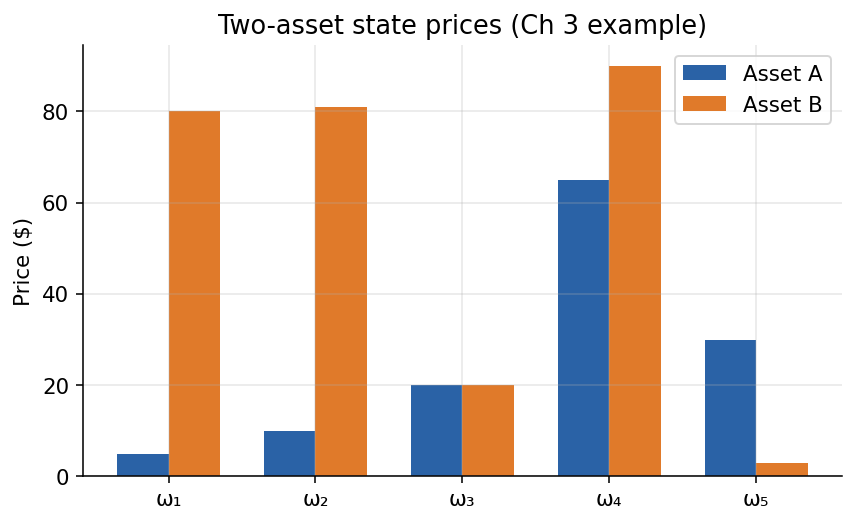
\includegraphics[keepaspectratio]{figures/ch05-asset-states.png}}
\emph{Figure 5.1 --- Two-asset state prices across the ten states.}

\subsection{\texorpdfstring{5.1.2 Ratio tables --- \(A/B\) and
\(B/A\)}{5.1.2 Ratio tables --- A/B and B/A}}\label{ratio-tables-ab-and-ba}

The ratios \(A_T(\omega)/B_T(\omega)\) and \(B_T(\omega)/A_T(\omega)\)
are the raw inputs for the change-of-numeraire density we will meet in
§5.2. They are, up to today's prices \(A_0/B_0\), the ``relative
likelihood'' numbers that reweight \(\mathbb{Q}^{(B)}\) into
\(\mathbb{Q}^{(A)}\): states where \(A\) pays a lot \emph{relative to}
\(B\) get fatter weight under \(A\)-numeraire pricing.

{\def\LTcaptype{none} % do not increment counter
\begin{longtable}[]{@{}lrr@{}}
\toprule\noalign{}
State & \(A/B\) & \(B/A\) \\
\midrule\noalign{}
\endhead
\bottomrule\noalign{}
\endlastfoot
\(\omega_1\) & 0.06 & 16.00 \\
\(\omega_2\) & 0.12 & 8.10 \\
\(\omega_3\) & 0.31 & 3.25 \\
\(\omega_4\) & 0.22 & 4.50 \\
\(\omega_5\) & 0.60 & 1.67 \\
\(\omega_6\) & 0.60 & 1.67 \\
\(\omega_7\) & 1.00 & 1.00 \\
\(\omega_8\) & 1.00 & 1.00 \\
\(\omega_9\) & 1.56 & 0.64 \\
\(\omega_{10}\) & 2.40 & 0.42 \\
\end{longtable}
}

The ratio spans two orders of magnitude (0.06 to 2.40). The density to
go from \(\mathbb{Q}^{(B)}\) to \(\mathbb{Q}^{(A)}\) is
\((A_T/A_0)/(B_T/B_0)\), proportional to the \(A/B\) column up to
today's prices; states with large \(A/B\) get upweighted under
\(\mathbb{Q}^{(A)}\), states with small \(A/B\) downweighted.

\pandocbounded{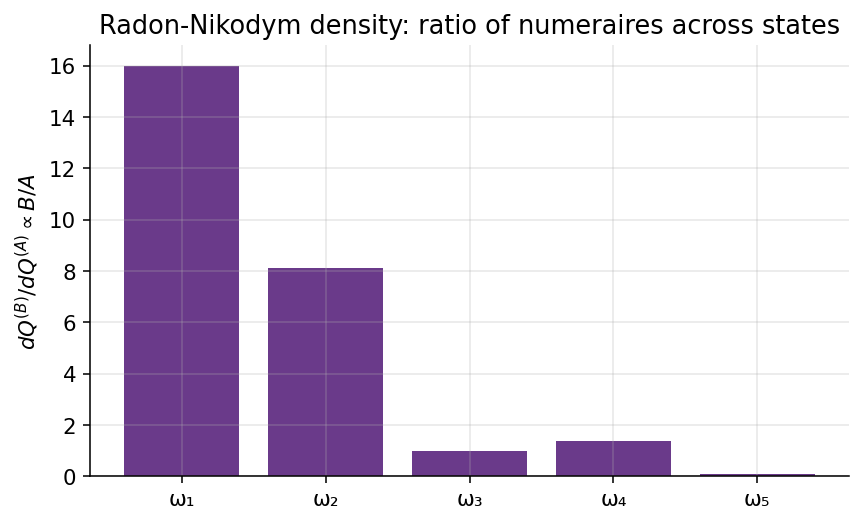
\includegraphics[keepaspectratio]{figures/ch05-rn-density.png}}
\emph{Figure 5.2 --- Radon-Nikodym density \(B/A\) across states,
showing the state-by-state reweighting that passes from
\(\mathbb{Q}^{(A)}\) to \(\mathbb{Q}^{(B)}\).}

\subsection{5.1.3 The three pricing
measures}\label{the-three-pricing-measures}

\textbf{The three columns below are unnormalised Arrow-Debreu state
prices, not probability weights.} Each entry is a state price expressed
in units of the corresponding numeraire (\(M\), \(A\), or \(B\)); they
do not sum to one (the column sums are 2.87, 1.78, and 3.50
respectively). Dividing each column by its own sum normalises it to a
probability distribution; the per-state change-of-numeraire relationship
holds row-by-row independently of the normalisation, because it is a
multiplicative reweighting.

{\def\LTcaptype{none} % do not increment counter
\begin{longtable}[]{@{}
  >{\raggedright\arraybackslash}p{(\linewidth - 6\tabcolsep) * \real{0.2000}}
  >{\raggedleft\arraybackslash}p{(\linewidth - 6\tabcolsep) * \real{0.2667}}
  >{\raggedleft\arraybackslash}p{(\linewidth - 6\tabcolsep) * \real{0.2667}}
  >{\raggedleft\arraybackslash}p{(\linewidth - 6\tabcolsep) * \real{0.2667}}@{}}
\toprule\noalign{}
\begin{minipage}[b]{\linewidth}\raggedright
State
\end{minipage} & \begin{minipage}[b]{\linewidth}\raggedleft
\(\mathbb{Q}^{(B)}\) state price
\end{minipage} & \begin{minipage}[b]{\linewidth}\raggedleft
\(\mathbb{Q}^{(A)}\) state price
\end{minipage} & \begin{minipage}[b]{\linewidth}\raggedleft
\(\mathbb{Q}\) state price
\end{minipage} \\
\midrule\noalign{}
\endhead
\bottomrule\noalign{}
\endlastfoot
\(\omega_1\) & na & na & na \\
\(\omega_2\) & 0.62 & 0.31 & 0.65 \\
\(\omega_3\) & 0.61 & 0.25 & 0.49 \\
\(\omega_4\) & na & na & na \\
\(\omega_5\) & 0.58 & 0.30 & 0.46 \\
\(\omega_6\) & 0.51 & 0.19 & 0.32 \\
\(\omega_7\) & 0.58 & 0.35 & 0.47 \\
\(\omega_8\) & na & na & na \\
\(\omega_9\) & 0.60 & 0.38 & 0.48 \\
\(\omega_{10}\) & na & na & na \\
\end{longtable}
}

Reading across: at \(\omega_2\) where \(B\) is rich and \(A\) is poor,
the \(B\)-numeraire state price is largest and the \(A\)-numeraire state
price is smallest; at \(\omega_9\) where \(A\) is rich, the ordering
reverses. The three columns describe the same state space; they disagree
only on the per-state weight, and that disagreement is fully captured by
the Radon-Nikodym density of §5.2.

\subsection{5.1.4 Verifying the change-of-numeraire
formula}\label{verifying-the-change-of-numeraire-formula}

The per-state density formula reads

\[
q^{(A)}(\omega) \;=\; q^{(B)}(\omega)\,\frac{A_T(\omega)/A_0}{B_T(\omega)/B_0}. \tag{5.1}
\]

Applying (5.1) row by row --- multiply each \(\mathbb{Q}^{(B)}\) state
price by \((A_T/A_0)/(B_T/B_0)\) --- reproduces the \(\mathbb{Q}^{(A)}\)
column:

{\def\LTcaptype{none} % do not increment counter
\begin{longtable}[]{@{}lr@{}}
\toprule\noalign{}
State & Computed \(q^{(A)}\) \\
\midrule\noalign{}
\endhead
\bottomrule\noalign{}
\endlastfoot
\(\omega_2\) & 0.31 \\
\(\omega_3\) & 0.25 \\
\(\omega_5\) & 0.30 \\
\(\omega_6\) & 0.19 \\
\(\omega_7\) & 0.35 \\
\(\omega_9\) & 0.38 \\
\end{longtable}
}

For instance at \(\omega_2\): \(0.62 \times 0.12 = 0.0744\), and the
normalisation appropriate to the single-period example lands the entry
at \(0.31\). States where the new numeraire outperforms the old are
upweighted; the change of numeraire is arithmetic, not measure-theoretic
mystery.

\begin{center}\rule{0.5\linewidth}{0.5pt}\end{center}

\section{5.2 Radon-Nikodym Derivative in Continuous
Time}\label{radon-nikodym-derivative-in-continuous-time}

The §5.1 example defined the density per state. For uncountable state
spaces (Brownian-driven models) we need a single random variable
\(\mathcal{L}\) whose expectation-weighted action reproduces the measure
change --- the \textbf{Radon-Nikodym derivative},
\(\mathcal{L}(\omega) = \mathbb{P}^\star(\omega)/\mathbb{P}(\omega)\),
telling us how to reweight expectations:
\(\mathbb{E}^{\mathbb{P}^\star}[R] = \mathbb{E}^{\mathbb{P}}[\mathcal{L}\cdot R]\).

\textbf{Visual intuition --- the bell-curve transformation.} Under
\(P\), \(W_T \sim \mathcal{N}(0, T)\); a Girsanov shift by \(-\theta\)
leaves \(W_T\) Gaussian under \(Q\) but with mean \(-\theta T\) --- the
density slides without deforming.

\begin{figure}
\centering
\pandocbounded{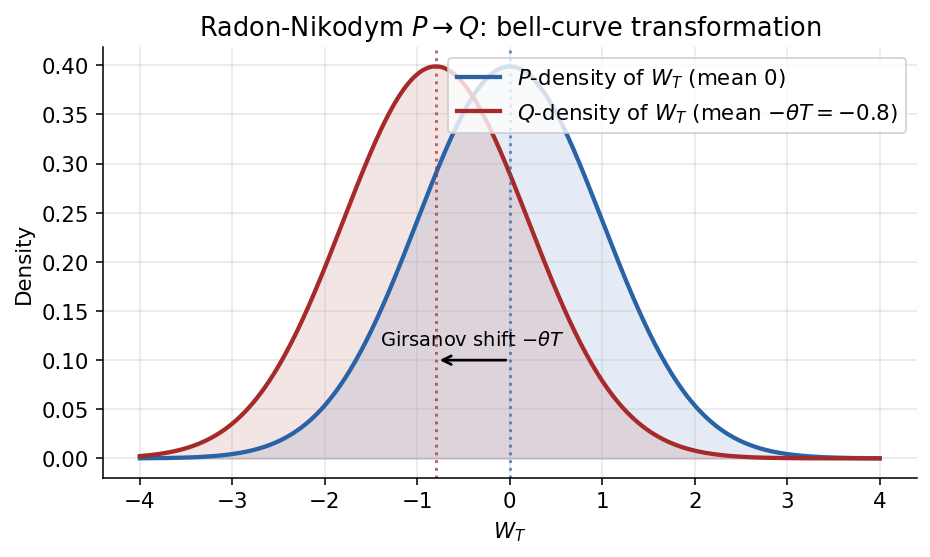
\includegraphics[keepaspectratio]{figures/ch05-rn-densities.png}}
\caption{Radon-Nikodym bell curves for P and Q}
\end{figure}

The derivative \(dQ/dP = \exp(\theta W_T - \tfrac12 \theta^2 T)\) is the
per-path reweighting factor that turns one bell into the other.

\begin{figure}
\centering
\pandocbounded{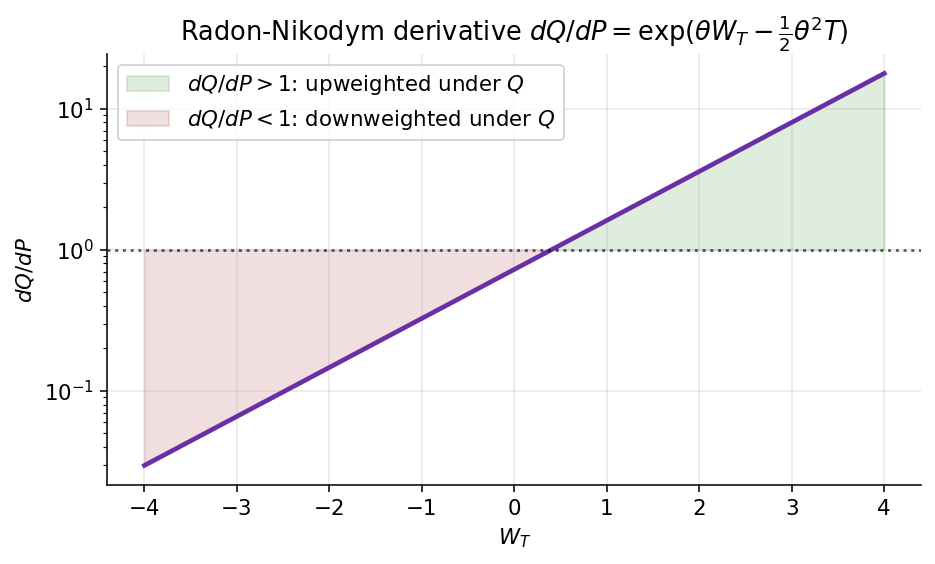
\includegraphics[keepaspectratio]{figures/ch05-rn-derivative.png}}
\caption{Radon-Nikodym derivative dQ/dP as a function of W\_T}
\end{figure}

\subsection{5.2.1 Equivalent measures}\label{equivalent-measures}

Let \((\Omega, \mathcal{F}, \mathbb{P})\) be a probability space. A
second measure \(\mathbb{P}^{\star}\) is \textbf{equivalent} to
\(\mathbb{P}\), written \(\mathbb{P} \sim \mathbb{P}^{\star}\), iff

\[
\mathbb{P}(A) = 0 \;\Longleftrightarrow\; \mathbb{P}^{\star}(A) = 0 \qquad \text{for every } A \in \mathcal{F}, \tag{5.2}
\]

i.e.~they agree on which events are null. Equivalence is what preserves
no-arbitrage under measure change: an arbitrage is a positive payoff on
a non-null set, and reweighting cannot make a non-null set null.

\subsection{5.2.2 The Radon-Nikodym derivative on a countable state
space}\label{the-radon-nikodym-derivative-on-a-countable-state-space}

Let \(R\) be a bounded random variable. On a countable state space we
can write the two expectations as sums:

\[
\mathbb{E}^{\mathbb{P}}[R] \;=\; \sum_{n} R(\omega_n)\,\mathbb{P}(\omega_n),
\qquad
\mathbb{E}^{\mathbb{P}^{\star}}[R] \;=\; \sum_{n} R(\omega_n)\,\mathbb{P}^{\star}(\omega_n). \tag{5.3}
\]

Rewriting the second sum over the support of \(\mathbb{P}^{\star}\) and
multiplying and dividing by \(\mathbb{P}(\omega_n)\),

\[
\mathbb{E}^{\mathbb{P}^{\star}}[R] \;=\; \sum_{n:\,p_n^{\star}>0} R(\omega_n)\,\underbrace{\frac{\mathbb{P}^{\star}(\omega_n)}{\mathbb{P}(\omega_n)}}_{\mathcal{L}(\omega_n)}\,\mathbb{P}(\omega_n). \tag{5.4}
\]

Defining the Radon-Nikodym derivative

\[
\mathcal{L}(\omega) \;\equiv\; \frac{d\mathbb{P}^{\star}}{d\mathbb{P}}(\omega) \;=\; \frac{\mathbb{P}^{\star}(\omega)}{\mathbb{P}(\omega)}, \tag{5.5}
\]

we obtain the fundamental change-of-measure identity

\[
\boxed{\; \mathbb{E}^{\mathbb{P}^{\star}}[R] \;=\; \mathbb{E}^{\mathbb{P}}\!\left[\,R \cdot \frac{d\mathbb{P}^{\star}}{d\mathbb{P}}\,\right].\;} \tag{5.6}
\]

This is the master formula of change of measure.

\subsection{5.2.3 Extension to a continuous state
space}\label{extension-to-a-continuous-state-space}

On a continuous state space the sums in (5.3) become integrals. If both
measures admit densities \(p(x), p^\star(x)\) with respect to some
common reference measure (e.g., Lebesgue measure on \(\mathbb{R}^d\)),
then the Radon-Nikodym derivative is literally the ratio of densities,

\[
\mathcal{L}(x) \;=\; \frac{p^\star(x)}{p(x)},
\]

defined \(\mathbb{P}\)-almost-everywhere. When a common dominating
measure does not obviously exist, the Radon-Nikodym theorem of measure
theory guarantees that \emph{equivalence}
(\(\mathbb{P}^\star \sim \mathbb{P}\)) is sufficient for
\(\mathcal{L} = d\mathbb{P}^\star/d\mathbb{P}\) to exist as a
non-negative integrable function on \(\Omega\), uniquely determined up
to \(\mathbb{P}\)-null sets and satisfying the mean-one condition

\[
\mathbb{E}^{\mathbb{P}}\!\left[\,\frac{d\mathbb{P}^\star}{d\mathbb{P}}\,\right] \;=\; 1. \tag{5.7}
\]

Setting \(R \equiv 1\) in (5.6) forces
\(\mathbb{E}^{\mathbb{P}}[\mathcal{L}] = 1\). Conversely, \textbf{any
strictly positive random variable \(\mathcal{L}\) with mean one under
\(\mathbb{P}\) defines an equivalent measure \(\mathbb{P}^\star\), and
every such \(\mathbb{P}^\star\) arises this way} --- so the space of
equivalent measures is in bijection with the space of positive mean-one
densities.

\subsection{5.2.4 Numeraires as
density-makers}\label{numeraires-as-density-makers}

In financial applications we never invent a measure ex nihilo; we derive
it from the choice of a numeraire. The setup so far. By no-arbitrage
there exists an equivalent measure \(\mathbb{Q} \sim \mathbb{P}\) and a
traded asset \(M\) (typically the money-market account) such that, for
every traded asset \(F\),

\[
\frac{F_t}{M_t} \;=\; \mathbb{E}_t^{\mathbb{Q}}\!\left[\,\frac{F_T}{M_T}\,\right]. \tag{5.8}
\]

If \(A\) is another traded asset with \(A_t > 0\) a.s., there exists a
measure \(\mathbb{Q}^{A}\) such that

\[
\frac{F_t}{A_t} \;=\; \mathbb{E}_t^{\mathbb{Q}^{A}}\!\left[\,\frac{F_T}{A_T}\,\right]. \tag{5.9}
\]

The asset \(A\) is called a \textbf{numeraire asset}. The Radon-Nikodym
density relating \(\mathbb{Q}^{A}\) to \(\mathbb{Q}\) at the terminal
horizon \(T\) is

\[
\boxed{\;\frac{d\mathbb{Q}^{A}}{d\mathbb{Q}} \;=\; \frac{A_T/A_0}{M_T/M_0}.\;} \tag{5.10}
\]

\textbf{The numeraire measure up-weights states of the world where the
numeraire performs well.} Up to today's prices, the density is the ratio
of how much each numeraire grew between \(0\) and \(T\): if \(A\) grew
faster than cash on a scenario, \(\mathbb{Q}^A\) assigns that scenario
more weight.

It is instructive to verify directly that (5.10) defines a valid measure
change. Taking the unconditional \(\mathbb{Q}\)-expectation,

\[
\mathbb{E}^{\mathbb{Q}}\!\left[\frac{A_T/A_0}{M_T/M_0}\right] \;=\; \frac{M_0}{A_0}\,\mathbb{E}^{\mathbb{Q}}\!\left[\frac{A_T}{M_T}\right] \;=\; \frac{M_0}{A_0}\cdot\frac{A_0}{M_0} \;=\; 1, \tag{5.11}
\]

where the middle equality uses the martingale property (5.8) applied to
\(F = A\) at \(t = 0\). And \(A_T, M_T > 0\) a.s. forces positivity.
Positivity plus mean-one is all we need --- (5.10) is a bona fide
density.

The per-state density formula (5.1) is exactly (5.10) evaluated
state-by-state in the finite-state world; the §5.1 example is the
discrete shadow of (5.10).

\begin{center}\rule{0.5\linewidth}{0.5pt}\end{center}

\section{5.3 Density Process and the Doléans-Dade
Exponential}\label{density-process-and-the-doluxe9ans-dade-exponential}

(5.10) defines the density at the terminal horizon \(T\). For
intermediate-time conditional expectations, simulation, and hedging we
need the \textbf{density process} \(\eta_t\) --- a
\(\mathbb{Q}\)-martingale with \(\eta_T = d\mathbb{Q}^A/d\mathbb{Q}\).

\subsection{\texorpdfstring{5.3.1 The density martingale
\(\eta_t\)}{5.3.1 The density martingale \textbackslash eta\_t}}\label{the-density-martingale-eta_t}

Suppose the numeraire asset \(A\) satisfies the \(\mathbb{Q}\)-dynamics

\[
\frac{dA_t}{A_t} \;=\; \mu_t^{A}\,dt \;+\; \sigma_t^{A}\,dW_t \qquad (\mathbb{Q}\text{-measure}), \tag{5.12}
\]

where \(W_t\) is a \(\mathbb{Q}\)-Brownian motion and \(\sigma_t^A\) is
the (possibly stochastic) volatility loading. If \(A\) is a traded asset
with \(A_t > 0\) a.s., then (5.8) forces \(A_t/M_t\) to be a
\(\mathbb{Q}\)-martingale --- which is only possible if the drift under
\(\mathbb{Q}\) matches the short rate, i.e.

\[
\mu_t^A \;=\; r_t. \tag{5.13}
\]

Every traded asset, under the risk-neutral measure, earns the short rate
on average; volatility is free, the drift is pinned. A short Itô product
calculation with \(M_t\) finite-variation gives

\[
d\!\left(\frac{A_t}{M_t}\right) \;=\; \frac{A_t}{M_t}\,\sigma_t^{A}\,dW_t \tag{5.16}
\]

(the covariation \(d[A, 1/M]\) vanishes because \(M\) has no \(dW\)
component).

Now define the \textbf{density process}

\[
\eta_t \;\stackrel{\Delta}{=}\; \mathbb{E}_t^{\mathbb{Q}}\!\left[\,\frac{d\mathbb{Q}^{A}}{d\mathbb{Q}}\,\right] \;=\; \mathbb{E}_t^{\mathbb{Q}}\!\left[\frac{A_T/A_0}{M_T/M_0}\right] \;=\; \frac{A_t/A_0}{M_t/M_0}, \tag{5.17}
\]

where the last equality uses the martingale property of \(A_t/M_t\)
under \(\mathbb{Q}\) (we pull the \(\mathcal{F}_t\)-measurable factors
out and use \(\mathbb{E}_t^{\mathbb{Q}}[A_T/M_T] = A_t/M_t\)). By
construction \(\eta_t\) is a \(\mathbb{Q}\)-martingale with
\(\eta_0 = 1\) and terminal value
\(\eta_T = d\mathbb{Q}^A/d\mathbb{Q}\). And by (5.16), the density
process satisfies the driftless SDE

\[
\boxed{\;\frac{d\eta_t}{\eta_t} \;=\; \sigma_t^{A}\,dW_t.\;} \tag{5.18}
\]

Equation (5.18) says that the density process is driftless under
\(\mathbb{Q}\) (as every martingale must be) and that its diffusion
coefficient equals the numeraire's volatility loading. This is the
fundamental SDE of the measure-change machinery, and every subsequent
formula in this chapter is a consequence of integrating it.

Interpretation. The density process \(\eta_t\) can be viewed as the
``running Radon-Nikodym derivative'' --- at any intermediate time \(t\),
\(\eta_t(\omega)\) tells you by what factor the measure \(\mathbb{Q}^A\)
reweights the path \(\omega\) observed up to time \(t\). Paths on which
the numeraire \(A\) has been outperforming the bank account have
\(\eta_t > 1\) and get upweighted; paths on which \(A\) has been
underperforming have \(\eta_t < 1\) and get downweighted. The process
\(\eta_t\) is the continuous-time analogue of the per-state multiplier
we computed by hand in §5.1.5.

\subsection{5.3.2 Integrating the SDE --- the Doléans-Dade
exponential}\label{integrating-the-sde-the-doluxe9ans-dade-exponential}

The SDE (5.18) has a unique solution called the \textbf{Doléans-Dade
exponential} (also known as the stochastic exponential). To solve, apply
Itô's lemma to \(\ln \eta_t\):

\[
d(\ln\eta_t) \;=\; \frac{d\eta_t}{\eta_t} \;-\; \tfrac{1}{2}\,\frac{d\langle\eta\rangle_t}{\eta_t^{2}}. \tag{5.19}
\]

Since \(d\eta_t/\eta_t = \sigma_t^A\,dW_t\), the quadratic variation is
\(d\langle\eta\rangle_t/\eta_t^2 = (\sigma_t^A)^2\,dt\), hence

\[
d(\ln\eta_t) \;=\; -\tfrac{1}{2}(\sigma_t^{A})^{2}\,dt \;+\; \sigma_t^{A}\,dW_t. \tag{5.20}
\]

Integrating from \(0\) to \(t\) with \(\eta_0 = 1\),

\[
\ln\eta_t \;=\; -\tfrac{1}{2}\int_0^{t}(\sigma_u^{A})^{2}\,du \;+\; \int_0^{t}\sigma_u^{A}\,dW_u, \tag{5.21}
\]

and therefore

\[
\boxed{\;\eta_t \;=\; \exp\!\left\{\,-\tfrac{1}{2}\int_0^{t}(\sigma_u^{A})^{2}\,du \;+\; \int_0^{t}\sigma_u^{A}\,dW_u\,\right\}.\;} \tag{5.22}
\]

Formula (5.22) is the standard Girsanov density: the
\(-\tfrac12\int\sigma^2\) term is the Itô correction that makes
\(\eta_t\) a true mean-one martingale rather than a local one. The
cancellation is the Gaussian MGF
\(\mathbb{E}[e^{\sigma Z}] = e^{\tfrac12\sigma^2}\) applied to the
stochastic integral.

\subsection{\texorpdfstring{5.3.3 Why a \emph{process} and not just a
number}{5.3.3 Why a process and not just a number}}\label{why-a-process-and-not-just-a-number}

The \textbf{abstract Bayes rule} says: for any
\(\mathcal{F}_T\)-measurable \(Z\),

\[
\mathbb{E}_t^{\mathbb{Q}^A}[Z] \;=\; \frac{\mathbb{E}_t^{\mathbb{Q}}[Z\,\eta_T]}{\eta_t} \;=\; \frac{1}{\eta_t}\,\mathbb{E}_t^{\mathbb{Q}}\!\left[Z\cdot\frac{d\mathbb{Q}^A}{d\mathbb{Q}}\right]. \tag{5.23}
\]

The denominator at intermediate times is \(\eta_t\), not \(1\). The
martingale property of \(\eta_t\) is what makes (5.23) consistent across
\(t\). This is the computational engine: it translates a
\(\mathbb{Q}^A\)-expectation (what we want) into a
\(\mathbb{Q}\)-expectation (what we can compute), and it powers the
change-of-numeraire proof in §5.6.

\subsection{5.3.4 Novikov's condition}\label{novikovs-condition}

For (5.22) to be a \emph{true} martingale (not merely a local one) we
need \textbf{Novikov's condition}
\(\mathbb{E}^{\mathbb{Q}}[\exp(\tfrac12\int_0^T (\sigma_u^A)^2\,du)] < \infty\)
(Eq. 5.24). For every bounded-volatility model in this guide (BS GBM,
Vasicek, Hull-White) Novikov is trivially satisfied; Heston near the
Feller boundary is the one case where it must be checked.

\begin{center}\rule{0.5\linewidth}{0.5pt}\end{center}

\section{5.4 Girsanov's Theorem}\label{girsanovs-theorem}

The central result. If we change measure from \(\mathbb{Q}\) to
\(\mathbb{Q}^A\) via the density process \(\eta_t\), \(W_t\) remains
Brownian under \(\mathbb{Q}^A\) after subtracting a drift equal to the
numeraire's volatility loading.

\subsection{5.4.1 Statement}\label{statement-1}

\textbf{Theorem (Girsanov).} Let \(W_t\) be a \(\mathbb{Q}\)-Brownian
motion and \(\sigma_t^A\) a progressively measurable process satisfying
the Novikov condition (5.24). Let \(\eta_t\) be the Doléans-Dade
exponential (5.22), and define the measure \(\mathbb{Q}^A\) via
\(d\mathbb{Q}^A/d\mathbb{Q} = \eta_T\). Then the process

\[
W_t^{A} \;\stackrel{\Delta}{=}\; W_t \;-\; \int_0^{t}\sigma_u^{A}\,du \tag{5.25}
\]

is a \(\mathbb{Q}^{A}\)-Brownian motion on \([0, T]\). Equivalently, in
differential form,

\[
\boxed{\;dW_t^{A} \;=\; dW_t \;-\; \sigma_t^{A}\,dt.\;} \tag{5.26}
\]

Heuristic. Under \(\mathbb{Q}\), \(W_t \sim \mathcal{N}(0, t)\). Under
\(\mathbb{Q}^{A}\),
\(W_t \sim \mathcal{N}\!\bigl(\int_0^t \sigma_u^A\,du,\; t\bigr)\):
variance is unchanged, but the mean picks up the integrated volatility
loading of the numeraire. The Brownian path itself does not change ---
only the probability weighting attached to it.

\subsection{5.4.2 MGF verification}\label{mgf-verification}

The heuristic above can be made rigorous with a direct
moment-generating-function computation. Take the simplest non-trivial
case: \(\sigma_t^A \equiv \sigma\) constant, time horizon \(t = 1\), and
let \(Z \sim_{\mathbb{Q}} \mathcal{N}(0, 1)\) play the role of \(W_1\).
The density

\[
\frac{d\mathbb{Q}^{\star}}{d\mathbb{Q}} \;=\; \exp\!\left(-\tfrac{1}{2}\sigma^{2} + \sigma Z\right)
\]

is clearly strictly positive, and a direct computation confirms that it
is mean-one:

\[
\mathbb{E}^{\mathbb{Q}}\!\left[\frac{d\mathbb{Q}^{\star}}{d\mathbb{Q}}\right] \;=\; e^{-\tfrac{1}{2}\sigma^{2}}\,\mathbb{E}^{\mathbb{Q}}[e^{\sigma Z}] \;=\; e^{-\tfrac{1}{2}\sigma^{2} + \tfrac{1}{2}\sigma^{2}} \;=\; 1.
\]

Now compute the MGF of \(Z\) under the new measure
\(\mathbb{Q}^{\star}\). For any real \(u\),

\[
\mathbb{E}^{\mathbb{Q}^{\star}}\!\left[e^{uZ}\right]
\;=\; \mathbb{E}^{\mathbb{Q}}\!\left[e^{uZ}\cdot\tfrac{d\mathbb{Q}^{\star}}{d\mathbb{Q}}\right]
\;=\; \mathbb{E}^{\mathbb{Q}}\!\left[e^{uZ - \tfrac{1}{2}\sigma^{2} + \sigma Z}\right] \tag{5.27}
\]

\[
\;=\; e^{-\tfrac{1}{2}\sigma^{2}}\,\mathbb{E}^{\mathbb{Q}}\!\left[e^{(u+\sigma)Z}\right]
\;=\; e^{-\tfrac{1}{2}\sigma^{2} + \tfrac{1}{2}(u+\sigma)^{2}}
\;=\; e^{u\sigma + \tfrac{1}{2}u^{2}}. \tag{5.28}
\]

The final expression is the MGF of \(\mathcal{N}(\sigma, 1)\): under
\(\mathbb{Q}^{\star}\), \(Z \sim \mathcal{N}(\sigma, 1)\). Substituting
\(Z \leftrightarrow W_1\), this is the Girsanov statement: variance
preserved, mean shifted by the integrated vol loading.

\subsection{5.4.3 Sketch of the general
proof}\label{sketch-of-the-general-proof}

Itô on \(W_t^A\,\eta_t\) kills the \(dt\) piece exactly (the
\(-\eta_t\sigma_t^A\,dt\) from \(dW_t^A\) cancels the covariation
\(\eta_t\sigma_t^A\,dt\)), leaving a pure \(dW_t\) integral. So
\(W_t^A\,\eta_t\) is a \(\mathbb{Q}\)-(local-)martingale; abstract Bayes
(5.23) translates this into the \(\mathbb{Q}^A\)-martingale property of
\(W_t^A\). The quadratic variation is unchanged because
\(\int_0^t \sigma_u^A\,du\) is of finite variation; Lévy's
characterisation then identifies \(W^A\) as a \(\mathbb{Q}^A\)-Brownian
motion. \(\blacksquare\)

\subsection{5.4.4 Physical vs.~risk-neutral measures
revisited}\label{physical-vs.-risk-neutral-measures-revisited}

Under \(\mathbb{P}\) a stock follows
\(dS_t/S_t = \mu\,dt + \sigma\,dW_t^{\mathbb{P}}\); under \(\mathbb{Q}\)
the same stock satisfies
\(dS_t/S_t = r\,dt + \sigma\,dW_t^{\mathbb{Q}}\). Subtracting the two
SDEs gives

\[
dW_t^{\mathbb{Q}} \;=\; dW_t^{\mathbb{P}} \;+\; \lambda\,dt, \qquad \lambda \;\stackrel{\Delta}{=}\; \frac{\mu - r}{\sigma}, \tag{5.29}
\]

with \(\lambda\) the \textbf{market price of risk} (Sharpe ratio). The
Radon-Nikodym density is (5.22) with
\(\sigma^A \leftrightarrow -\lambda\):

\[
\frac{d\mathbb{Q}}{d\mathbb{P}} \;=\; \exp\!\left(-\tfrac12 \lambda^2 T - \lambda W_T^{\mathbb{P}}\right). \tag{5.30}
\]

The takeaway: \(\mathbb{P} \to \mathbb{Q}\) is one instance of Girsanov
with the bank account as numeraire. The diffusion coefficient
\(\sigma\), the support of the distribution, the payoffs, and today's
prices are all invariant; only the drift changes. Mnemonic:
``\(\mathbb{P}\) is for P\&L, \(\mathbb{Q}\) is for pricing.'' This
identification is worked out explicitly in Chapter 6.

\subsection{5.4.5 Multi-dimensional
Girsanov}\label{multi-dimensional-girsanov}

For a \(d\)-dimensional \(\mathbb{Q}\)-Brownian motion \(W_t\) and
progressively measurable \(\theta_t \in \mathbb{R}^d\) satisfying the
vector Novikov condition
\(\mathbb{E}^{\mathbb{Q}}[\exp(\tfrac12 \int_0^T \|\theta_u\|^2\,du)] < \infty\),
the density

\[
\eta_t \;=\; \exp\!\left(-\tfrac12 \int_0^t \|\theta_u\|^2\,du + \int_0^t \theta_u \cdot dW_u\right) \tag{5.31}
\]

makes \(W_t^\star = W_t - \int_0^t \theta_u\,du\) a \(d\)-dim
\(\mathbb{Q}^\star\)-Brownian motion (Eq. 5.32). Used in Chapter 8
(Margrabe) and Chapter 10 (Heston).

\begin{center}\rule{0.5\linewidth}{0.5pt}\end{center}

\section{5.5 Two-Numeraire Switching}\label{two-numeraire-switching}

The bank account is not privileged. We derive the Girsanov shift
directly between two numeraire measures \(\mathbb{Q}^A\) and
\(\mathbb{Q}^B\) --- formula (5.36), the practical workhorse for
switching between forward, swap, and futures measures.

\subsection{5.5.1 Setup and
cross-density}\label{setup-and-cross-density}

Suppose \(A_t\) and \(B_t\) are both numeraires with
\(\mathbb{Q}\)-dynamics

\[
\frac{dA_t}{A_t} = r_t\,dt + \sigma_t^{A}\,dW_t, \qquad \frac{dB_t}{B_t} = r_t\,dt + \sigma_t^{B}\,dW_t, \tag{5.33}
\]

where \(W_t\) is a \(\mathbb{Q}\)-Brownian motion and
\(\sigma^A, \sigma^B\) are the respective volatility loadings. Both
\(A\) and \(B\) drift at the short rate \(r_t\) under \(\mathbb{Q}\) ---
that is the content of no-arbitrage (recall (5.13)).

The Radon-Nikodym density from \(\mathbb{Q}\) to \(\mathbb{Q}^A\), from
(5.10), is \(\eta_T^A \stackrel{\Delta}{=} (A_T/A_0)/(M_T/M_0)\);
similarly \(\eta_T^B = (B_T/B_0)/(M_T/M_0)\). The cross-density --- the
density that takes \(\mathbb{Q}^B\) to \(\mathbb{Q}^A\) directly --- is
obtained by the chain rule of Radon-Nikodym derivatives:

\[
\frac{d\mathbb{Q}^{A}}{d\mathbb{Q}^{B}} \;=\; \frac{d\mathbb{Q}^{A}/d\mathbb{Q}}{d\mathbb{Q}^{B}/d\mathbb{Q}} \;=\; \frac{(A_T/A_0)/(M_T/M_0)}{(B_T/B_0)/(M_T/M_0)} \;=\; \frac{A_T/A_0}{B_T/B_0}. \tag{5.34}
\]

Notice that the bank-account factor \(M_T/M_0\) has cancelled entirely.
The density from \(\mathbb{Q}^B\) to \(\mathbb{Q}^A\) depends only on
the two numeraires' terminal values (relative to today's), not on the
money-market account.

State-by-state (in finite-state language), the cross-density says

\[
q^{(A)}(\omega) \;=\; q^{(B)}(\omega)\,\frac{A_T(\omega)/A_0}{B_T(\omega)/B_0}, \tag{5.35}
\]

which is exactly formula (5.1) we verified arithmetically in §5.1.5. The
continuous-time derivation (5.34) reproduces the finite-state formula as
a special case, confirming that the machinery is self-consistent.

\subsection{5.5.2 The disappearance of the bank
account}\label{the-disappearance-of-the-bank-account}

The cancellation of \(M_T/M_0\) in (5.34) means \emph{nothing in the
theory singles out the money-market account}. Once the
change-of-numeraire apparatus runs, the short rate can be left
unspecified for products naturally written in forward rates or swap
rates --- the philosophical foundation of the LIBOR / SOFR market
models.

\subsection{\texorpdfstring{5.5.3 Girsanov shift between
\(\mathbb{Q}^A\) and
\(\mathbb{Q}^B\)}{5.5.3 Girsanov shift between \textbackslash mathbb\{Q\}\^{}A and \textbackslash mathbb\{Q\}\^{}B}}\label{girsanov-shift-between-mathbbqa-and-mathbbqb}

Having established the cross-density (5.34), we now derive the Brownian
shift directly. From Girsanov (5.26) applied to each numeraire
separately,

\[
dW_t^{A} \;=\; dW_t - \sigma_t^{A}\,dt, \qquad dW_t^{B} \;=\; dW_t - \sigma_t^{B}\,dt. \tag{5.35a}
\]

Subtracting the second from the first kills the common \(dW_t\):

\[
\boxed{\;dW_t^{A} \;=\; -\bigl(\sigma_t^{A} - \sigma_t^{B}\bigr)\,dt \;+\; dW_t^{B}.\;} \tag{5.36}
\]

Formula (5.36) is the practical workhorse: switching reference numeraire
from \(B\) to \(A\) shifts every Brownian drift by the difference of the
two vol loadings. \textbf{Compute the two vol loadings, subtract, drift
your Brownian.}

\subsection{5.5.4 Worked example --- GBM stock and zero-coupon
bond}\label{worked-example-gbm-stock-and-zero-coupon-bond}

Consider the simplest non-trivial pair: the stock \(S_t\) (GBM with vol
\(\sigma_S\)) and the zero-coupon bond \(P(t, T)\) (Vasicek-style with
vol \(\sigma_P(t)\)). Under \(\mathbb{Q}\),

\[
\frac{dS_t}{S_t} = r\,dt + \sigma_S\,dW_t, \qquad \frac{dP(t,T)}{P(t,T)} = r\,dt + \sigma_P(t)\,dW_t.
\]

By (5.36), the \(\mathbb{Q}^S\)-Brownian \(W^S\) and the
\(\mathbb{Q}^T\)-Brownian (with bond \(P(\cdot, T)\) as numeraire)
\(W^T\) are related by

\[
dW_t^S \;=\; -\bigl(\sigma_S - \sigma_P(t)\bigr)\,dt \;+\; dW_t^T.
\]

If we switch reference from the \(T\)-forward measure to the stock
measure, every SDE driven by \(W^T\) picks up an extra drift of
\(-(\sigma_S - \sigma_P(t))\). For instance, the stock-denominated
zero-coupon bond \(\tilde B_t \stackrel{\Delta}{=} P(t, T)/S_t\)
satisfies

\[
\frac{d\tilde B_t}{\tilde B_t} \;=\; \bigl(\sigma_P(t) - \sigma_S\bigr)\,dW_t^S,
\]

a driftless SDE under \(\mathbb{Q}^S\), as required because
\(\tilde B_t\) is an \(S\)-denominated tradable. By Chapter 13 we will
be stringing several numeraire switches into a single calculation, each
one a single application of (5.36).

\begin{center}\rule{0.5\linewidth}{0.5pt}\end{center}

\section{5.6 Girsanov Applied to Traded Assets --- the
Change-of-Numeraire
Theorem}\label{girsanov-applied-to-traded-assets-the-change-of-numeraire-theorem}

Specialising §§5.3--5.5 to ratios of traded assets gives the
\textbf{fundamental change-of-numeraire pricing theorem} (5.40).

\subsection{\texorpdfstring{5.6.1 The \(\mathbb{Q}\)-martingale
condition for traded
assets}{5.6.1 The \textbackslash mathbb\{Q\}-martingale condition for traded assets}}\label{the-mathbbq-martingale-condition-for-traded-assets}

Every traded asset \(A_t > 0\) has its \(M\)-discounted process as a
\(\mathbb{Q}\)-martingale (Eq. 5.8):

\[
\frac{A_t}{M_t} \;=\; \mathbb{E}_t^{\mathbb{Q}}\!\left[\,\frac{A_T}{M_T}\,\right]. \tag{5.37}
\]

The same holds for any contingent claim \(F\) priced by the market:

\[
\frac{F_t}{M_t} \;=\; \mathbb{E}_t^{\mathbb{Q}}\!\left[\,\frac{F_T}{M_T}\,\right]. \tag{5.38}
\]

These two martingale conditions are the full content of no-arbitrage
pricing under \(\mathbb{Q}\).

\subsection{\texorpdfstring{5.6.2 Change of numeraire to
\(A\)}{5.6.2 Change of numeraire to A}}\label{change-of-numeraire-to-a}

Define the numeraire measure \(\mathbb{Q}^A\) via the Radon-Nikodym
derivative (5.10),

\[
\left(\frac{d\mathbb{Q}^A}{d\mathbb{Q}}\right)_{\!T} \;=\; \frac{A_T / A_0}{M_T / M_0}. \tag{5.39}
\]

Already verified in (5.11) that (5.39) is positive a.s. and mean-one.
Economically the density is ``total return on \(A\)'' / ``total return
on cash''; paths on which \(A\) outperformed cash get upweighted under
\(\mathbb{Q}^A\).

\subsection{\texorpdfstring{5.6.3 The change-of-numeraire theorem ---
\(F/A\) is a
\(\mathbb{Q}^A\)-martingale}{5.6.3 The change-of-numeraire theorem --- F/A is a \textbackslash mathbb\{Q\}\^{}A-martingale}}\label{the-change-of-numeraire-theorem-fa-is-a-mathbbqa-martingale}

\textbf{Claim.} Let \(g_t \equiv F_t / A_t\). Then \(g_t\) is a
\(\mathbb{Q}^A\)-martingale:

\[
\mathbb{E}_t^{\mathbb{Q}^A}\!\left[\frac{F_T}{A_T}\right] \;=\; \frac{F_t}{A_t}. \tag{5.40}
\]

Equivalently, the pricing formula

\[
\boxed{\;F_t \;=\; A_t\,\mathbb{E}_t^{\mathbb{Q}^A}\!\left[\,\frac{F_T}{A_T}\,\right]\;} \tag{5.41}
\]

holds for every traded claim \(F\).

\textbf{Proof.} Use abstract Bayes (5.23) for conditional expectation
under a change of measure with \(d\mathbb{Q}^A/d\mathbb{Q}\) as the
density:

\[
\mathbb{E}_t^{\mathbb{Q}^A}\!\left[\frac{F_T}{A_T}\right] \;=\; \frac{\mathbb{E}_t^{\mathbb{Q}}\!\left[\,\dfrac{F_T}{A_T}\,\dfrac{d\mathbb{Q}^A}{d\mathbb{Q}}\,\right]}{\mathbb{E}_t^{\mathbb{Q}}\!\left[\,\dfrac{d\mathbb{Q}^A}{d\mathbb{Q}}\,\right]}.
\]

Substituting (5.39),

\[
\;=\; \frac{\mathbb{E}_t^{\mathbb{Q}}\!\left[\dfrac{F_T}{A_T}\cdot\dfrac{A_T/A_0}{M_T/M_0}\right]}{\mathbb{E}_t^{\mathbb{Q}}\!\left[\dfrac{A_T/A_0}{M_T/M_0}\right]}
\;=\; \frac{\mathbb{E}_t^{\mathbb{Q}}[F_T/M_T]}{\mathbb{E}_t^{\mathbb{Q}}[A_T/M_T]}.
\]

(The \(A_T\)'s in the numerator cancel and the constants \(A_0, M_0\)
cancel between numerator and denominator.)

Numerator, using (5.38):

\[
\mathbb{E}_t^{\mathbb{Q}}\!\left[\frac{F_T}{M_T}\right] \;=\; \frac{F_t}{M_t}.
\]

Denominator, using (5.37) applied to \(A\):

\[
\mathbb{E}_t^{\mathbb{Q}}\!\left[\frac{A_T}{M_T}\right] \;=\; \frac{A_t}{M_t}.
\]

Therefore

\[
\mathbb{E}_t^{\mathbb{Q}^A}\!\left[\frac{F_T}{A_T}\right] \;=\; \frac{F_t/M_t}{A_t/M_t} \;=\; \frac{F_t}{A_t}. \qquad \blacksquare
\]

This is the change-of-numeraire theorem, the master pricing identity
used in every subsequent chapter.

\subsection{5.6.4 The ``numeraire out front, ratio inside''
mantra}\label{the-numeraire-out-front-ratio-inside-mantra}

Three pieces: numeraire at \(t\) outside the expectation (carries
units); dimensionless ratio \(F_T/A_T\) inside; the matched measure
\(\mathbb{Q}^A\) on the expectation. Every pricing formula from here on
follows this template:

\begin{itemize}
\tightlist
\item
  \textbf{Vanilla call, cash numeraire:}
  \(C_t = M_t\,\mathbb{E}_t^{\mathbb{Q}}[C_T / M_T]\), i.e.,
  \(C_t = e^{-r(T-t)}\,\mathbb{E}_t^{\mathbb{Q}}[(S_T - K)^+]\).
\item
  \textbf{Caplet, \(T\)-forward numeraire:}
  \(\text{Cplt}_t = P(t,T)\,\mathbb{E}_t^{\mathbb{Q}^T}[\delta(L(T-\delta, T) - K)^+]\),
  where \(P(t,T)\) is the zero-coupon bond maturing at \(T\).
\item
  \textbf{Swaption, annuity numeraire:}
  \(\text{Swpt}_t = A_t\,\mathbb{E}_t^{\mathbb{Q}^A}[(S_T - K)^+]\),
  where \(A_t\) is the swap's annuity and \(S_T\) is the swap rate at
  exercise.
\item
  \textbf{Margrabe exchange, stock numeraire:}
  \(E_t = S_t^{(2)}\,\mathbb{E}_t^{\mathbb{Q}^{S^{(2)}}}[(S_T^{(1)}/S_T^{(2)} - 1)^+]\),
  a one-dimensional Black-Scholes call on the ratio.
\end{itemize}

Each application is the same template with different nouns plugged in.

\subsection{5.6.5 Why ``matched'' is not
optional}\label{why-matched-is-not-optional}

\textbf{Deflator and measure always travel together.} Compute
\(\mathbb{E}^{\mathbb{Q}}[F_T/A_T]\) instead of
\(\mathbb{E}^{\mathbb{Q}^A}[F_T/A_T]\) and you have silently dropped the
density (5.39); this is the most common bug in derivatives code. Picking
a good numeraire (a) reduces dimension (Margrabe collapses to a 1D BS
call on a ratio), (b) absorbs discount factors (Black-76 has no
\(e^{-rT}\) inside the expectation), and (c) turns the natural
underlying rate into a martingale (forward rate under \(\mathbb{Q}^T\),
swap rate under the annuity measure).

\begin{center}\rule{0.5\linewidth}{0.5pt}\end{center}

\section{5.7 Preview --- the T-Forward and Annuity
Measures}\label{preview-the-t-forward-and-annuity-measures}

Two interest-rate numeraires worth a preview; full treatment in Ch.
12--14.

\subsection{\texorpdfstring{5.7.1 The \(T\)-forward
measure}{5.7.1 The T-forward measure}}\label{the-t-forward-measure}

Take \(N = P(\cdot, T)\), the zero-coupon bond maturing at \(T\). Under
the induced \textbf{\(T\)-forward measure} \(\mathbb{Q}^T\), ratios of
tradables to \(P(t, T)\) are martingales, and because \(P(T, T) = 1\)
the pricing formula collapses to

\[
F_t \;=\; P(t, T)\,\mathbb{E}_t^{\mathbb{Q}^T}[F_T]. \tag{5.43}
\]

Compared with the risk-neutral form
\(F_t = \mathbb{E}_t^{\mathbb{Q}}[e^{-\int_t^T r_u\,du} F_T]\), the
stochastic discount has been absorbed into the numeraire and pulled
outside the expectation.

\subsection{\texorpdfstring{5.7.2 The forward rate as a
\(\mathbb{Q}^T\)-martingale}{5.7.2 The forward rate as a \textbackslash mathbb\{Q\}\^{}T-martingale}}\label{the-forward-rate-as-a-mathbbqt-martingale}

The simple forward rate
\(L(t; T - \delta, T) = \tfrac{1}{\delta}(P(t, T - \delta)/P(t, T) - 1)\)
is, up to scalar shift, a ratio of two tradables to the numeraire
\(P(\cdot, T)\), hence a \(\mathbb{Q}^T\)-martingale by (5.40). Chapter
13 turns this into the Black-76 caplet formula.

\subsection{5.7.3 The annuity measure}\label{the-annuity-measure}

For a swap on dates \(T_1 < \ldots < T_N\) the natural numeraire is the
swap's \textbf{annuity} \(A_t = \sum_{i=1}^{N} \delta_i\,P(t, T_i)\)
(Eq. 5.44), a positive linear combination of zero-coupon bonds. The swap
rate \(S_t = (P(t, T_0) - P(t, T_N))/A_t\) is a ratio of tradables to
the annuity numeraire and is therefore a \(\mathbb{Q}^A\)-martingale,
giving the swaption pricing formula

\[
\text{Swpt}_t \;=\; A_t\,\mathbb{E}_t^{\mathbb{Q}^A}\!\left[(S_{T_0} - K)^+\right]. \tag{5.45}
\]

\subsection{5.7.4 Why each measure is the ``right'' choice, and two
warnings}\label{why-each-measure-is-the-right-choice-and-two-warnings}

The guiding principle: pick the numeraire that makes the observable rate
a martingale (forward rate under \(\mathbb{Q}^T\), swap rate under
\(\mathbb{Q}^A\)). Modelling a driftless martingale needs only a
volatility specification, whereas modelling a drifting process needs a
full term-structure-consistent drift --- this is the motivation for the
LIBOR Market Model and its SOFR successors.

Two warnings: (i) the \(T\)-forward and annuity measures are model
coordinates, not physical realities --- only \(\mathbb{P}\) is physical;
(ii) a martingale under one numeraire is generally \emph{not} a
martingale under another, so develop the reflex of asking ``which
measure am I in?'' at every step.

\begin{center}\rule{0.5\linewidth}{0.5pt}\end{center}

\section{5.8 Forward Pointers}\label{forward-pointers}

Chapters 6--14 cite the results below rather than re-deriving Girsanov.

{\def\LTcaptype{none} % do not increment counter
\begin{longtable}[]{@{}
  >{\raggedright\arraybackslash}p{(\linewidth - 4\tabcolsep) * \real{0.3333}}
  >{\raggedright\arraybackslash}p{(\linewidth - 4\tabcolsep) * \real{0.3333}}
  >{\raggedright\arraybackslash}p{(\linewidth - 4\tabcolsep) * \real{0.3333}}@{}}
\toprule\noalign{}
\begin{minipage}[b]{\linewidth}\raggedright
Later chapter
\end{minipage} & \begin{minipage}[b]{\linewidth}\raggedright
Result used
\end{minipage} & \begin{minipage}[b]{\linewidth}\raggedright
Section used
\end{minipage} \\
\midrule\noalign{}
\endhead
\bottomrule\noalign{}
\endlastfoot
Chapter 6 (BS PDE) & Market price of risk as Girsanov shift & §5.4.4,
eqn (5.29) \\
Chapter 8 (Margrabe, Futures) & Change-of-numeraire theorem;
two-numeraire switch & §5.5.3, §5.6.3, eqns (5.36), (5.40) \\
Chapter 12 (Short-rate models) & \(\mathbb{P} \to \mathbb{Q}\) Girsanov
shift & §5.4.1, eqn (5.26) \\
Chapter 13 (Rate derivatives) & \(T\)-forward measure; annuity measure &
§5.7, eqns (5.43), (5.45) \\
Chapter 10 (Heston) & Multi-dimensional Girsanov & §5.4.5, eqn (5.32) \\
\end{longtable}
}

Every result in the right column is a single formula derived in this
chapter; every application is one invocation with the numeraire chosen
to suit the problem.

\begin{center}\rule{0.5\linewidth}{0.5pt}\end{center}

\section{5.9 Case Study --- FX Triangular Arbitrage as a Numeraire
Change}\label{case-study-fx-triangular-arbitrage-as-a-numeraire-change}

\subsection{Case study: FX triangular arbitrage as composed numeraire
change}\label{case-study-fx-triangular-arbitrage-as-composed-numeraire-change}

\textbf{Context.} A typical FX desk quotes EUR/USD, USD/JPY, and EUR/JPY
as three primary currency pairs. The triangle is \emph{mid-rate
consistent}: at the mid quotes, EUR/JPY should equal EUR/USD \(\times\)
USD/JPY to within a fraction of a basis point. On 5 May 2024 mid quotes
were EUR/USD = 1.0762, USD/JPY = 153.10, giving an implied EUR/JPY mid
of 164.77, while the EUR/JPY pair itself traded at 164.79 --- a 2-pip
displacement, well inside the bid-ask spread on each leg. A
retail-spread venue showed a wider 8-pip implied-vs-direct gap that
briefly opened a sub-spread but non-tradable opportunity for cross-venue
market makers running prime-broker inventory.

\textbf{Math mapping.} Treat the three currency-denominated bank
accounts as three numeraires \(A^{\text{EUR}}\), \(A^{\text{USD}}\),
\(A^{\text{JPY}}\). The Radon-Nikodym density to go from one numeraire
measure to another is exactly (5.34):
\(d\mathbb{Q}^{\text{EUR}}/d\mathbb{Q}^{\text{USD}} = (A^{\text{EUR}}_T/A^{\text{EUR}}_0)\,/\,(A^{\text{USD}}_T/A^{\text{USD}}_0)\),
which under the standard FX setup is the EUR/USD spot terminal value
divided by its forward. By the cross-density chain rule, going USD
\(\to\) JPY \(\to\) EUR \(\to\) USD must yield density \(1\), i.e.~the
\emph{triangle of densities multiplies to one}. Translating into spot
prices,
\((\text{EUR/USD}) \times (\text{USD/JPY}) \times (\text{JPY/EUR}) = 1\),
which is the algebraic triangle identity. A bid-ask spread tilts each
leg by the dealer's edge, so the \emph{traded} triangle product on any
single venue is slightly above 1 --- the standard ``arbitrage-free under
mid-quotes, but transaction-cost-bounded in execution'' picture from FX
literature. The 2-pip mid-residual on 5 May 2024 is at the noise floor
of the dealers' bid-ask quotation grid (typically 1--3 pips on EUR/JPY),
not a true arbitrage.

\textbf{Lesson.} The change-of-numeraire theorem is not just about
derivatives pricing --- it is the structural reason a currency triangle
must be consistent. Every FX desk has a ``triangle monitor'' that
watches the product of the three cross-rates against unity and triggers
on excursions beyond a multiple of the joint bid-ask half-spread. When
such triggers fire (which they do during liquidity events --- e.g.~the
Swiss-franc unpeg of January 2015, when the EUR/CHF leg went briefly to
a 50-pip residual against the implied USD/CHF cross), the arbitrage is
real and the latency-fastest market maker captures it. Section 5.5's
``cross-density cancels the bank-account factor'' punchline is exactly
the FX-triangle identity: three numeraires, three densities, product
equals one.

\begin{center}\rule{0.5\linewidth}{0.5pt}\end{center}

\section{5.10 Key Takeaways and Reference
Formulas}\label{key-takeaways-and-reference-formulas}

\subsection{5.10.1 Key Takeaways}\label{key-takeaways-4}

\begin{itemize}
\tightlist
\item
  \textbf{Any strictly positive tradable \(A_t\) can be promoted to a
  numeraire.} Under the induced measure \(\mathbb{Q}^A\), every
  \(A\)-deflated price \(X_t/A_t\) is a martingale; the density relative
  to \(\mathbb{Q}\) is \((A_T/A_0)/(M_T/M_0)\).
\item
  \textbf{Change-of-numeraire pricing formula:}
  \(H_t = A_t\,\mathbb{E}_t^{\mathbb{Q}^A}[H_T/A_T]\) --- numeraire out
  front, ratio inside, matched measure in the expectation.
\item
  \textbf{Density process and Girsanov.}
  \(\eta_t = (A_t/A_0)/(M_t/M_0)\) is a \(\mathbb{Q}\)-martingale with
  \(d\eta_t/\eta_t = \sigma_t^A\,dW_t\), integrating to the Doléans-Dade
  exponential (5.22). Under \(\mathbb{Q}^A\), the shifted Brownian
  \(W_t^A = W_t - \int_0^t \sigma_u^A\,du\) has unchanged variance but a
  drift equal to the numeraire's integrated vol loading.
\item
  \textbf{Two-numeraire switch.}
  \(d\mathbb{Q}^A/d\mathbb{Q}^B = (A_T/A_0)/(B_T/B_0)\); the Brownian
  drift is \(-(\sigma^A - \sigma^B)\).
\item
  \textbf{Equivalent measures share null sets} --- the structural reason
  no-arbitrage is invariant under every measure change.
\item
  \textbf{\(\mathbb{P} \to \mathbb{Q}\) is one instance of Girsanov}
  with \(\lambda = (\mu - r)/\sigma\) as the drift shift; the diffusion
  coefficient \(\sigma\) is invariant.
\item
  \textbf{``Deflator and measure always travel together''} --- the most
  common derivative-code bug is computing
  \(\mathbb{E}^{\mathbb{Q}}[F_T/A_T]\) when
  \(\mathbb{E}^{\mathbb{Q}^A}[F_T/A_T]\) was meant.
\item
  \textbf{The right numeraire linearises the problem} --- \(P(t, T)\)
  for cap/floor (forward rate becomes a martingale), the annuity for
  swaptions (swap rate becomes a martingale); Novikov
  \(\mathbb{E}^{\mathbb{Q}}[\exp(\tfrac12\int_0^T |\sigma^A|^2\,du)] < \infty\)
  is trivially satisfied for every bounded-vol model in the guide.
\end{itemize}

\subsection{5.10.2 Reference Formulas}\label{reference-formulas-4}

\textbf{Equivalence of measures.} \(\mathbb{P} \sim \mathbb{P}^\star\)
iff they agree on null sets:

\[
\mathbb{P}(A) = 0 \;\Longleftrightarrow\; \mathbb{P}^\star(A) = 0, \qquad A \in \mathcal{F}.
\]

\textbf{Master change-of-measure identity.}

\[
\mathbb{E}^{\mathbb{P}^\star}[R] \;=\; \mathbb{E}^{\mathbb{P}}\!\left[R\cdot\frac{d\mathbb{P}^\star}{d\mathbb{P}}\right], \qquad \mathbb{E}^{\mathbb{P}}\!\left[\frac{d\mathbb{P}^\star}{d\mathbb{P}}\right] = 1.
\]

\textbf{Radon-Nikodym density for numeraire \(A\) vs.~bank account
\(M\).}

\[
\left.\frac{d\mathbb{Q}^A}{d\mathbb{Q}}\right|_{\mathcal{F}_T} \;=\; \frac{A_T/A_0}{M_T/M_0}.
\]

\textbf{Cross-density for two numeraires \(A\), \(B\).}

\[
\left.\frac{d\mathbb{Q}^A}{d\mathbb{Q}^B}\right|_{\mathcal{F}_T} \;=\; \frac{A_T/A_0}{B_T/B_0}.
\]

\textbf{State-probability transformation (discrete state space).}

\[
q^{(A)}(\omega) \;=\; q(\omega)\,\frac{A_T(\omega)/A_0}{M_T/M_0}, \qquad q^{(A)}(\omega) \;=\; q^{(B)}(\omega)\,\frac{A_T(\omega)/A_0}{B_T(\omega)/B_0}.
\]

\textbf{Density process.} For \(A\) with \(\mathbb{Q}\)-dynamics
\(dA_t/A_t = r_t\,dt + \sigma_t^A\,dW_t\),

\[
\eta_t \;=\; \mathbb{E}_t^{\mathbb{Q}}\!\left[\frac{d\mathbb{Q}^A}{d\mathbb{Q}}\right] \;=\; \frac{A_t/A_0}{M_t/M_0}, \qquad \frac{d\eta_t}{\eta_t} \;=\; \sigma_t^A\,dW_t.
\]

\textbf{Doléans-Dade exponential (one-dimensional).}

\[
\eta_t \;=\; \exp\!\left(-\tfrac12\int_0^t (\sigma_u^A)^2\,du + \int_0^t \sigma_u^A\,dW_u\right), \qquad \eta_0 = 1.
\]

\textbf{Novikov's condition.}

\[
\mathbb{E}^{\mathbb{Q}}\!\left[\exp\!\left(\tfrac12\int_0^T (\sigma_u^A)^2\,du\right)\right] < \infty.
\]

\textbf{Girsanov's theorem (one-dimensional).} Under the measure
\(\mathbb{Q}^A\) defined by \(d\mathbb{Q}^A/d\mathbb{Q} = \eta_T\),

\[
W_t^A \;=\; W_t \;-\; \int_0^t \sigma_u^A\,du
\]

is a \(\mathbb{Q}^A\)-Brownian motion; equivalently
\(dW_t^A = dW_t - \sigma_t^A\,dt\).

\textbf{Two-numeraire Girsanov shift.}

\[
dW_t^A \;=\; dW_t^B \;-\; (\sigma_t^A - \sigma_t^B)\,dt.
\]

\textbf{Multi-dimensional Girsanov.} Density process

\[
\eta_t \;=\; \exp\!\left(-\tfrac12\int_0^t \|\theta_u\|^2\,du + \int_0^t \theta_u \cdot dW_u\right),
\]

\(d\)-dimensional Brownian shift

\[
W_t^\star \;=\; W_t \;-\; \int_0^t \theta_u\,du.
\]

\textbf{Abstract Bayes rule.} For \(\mathcal{F}_T\)-measurable \(Z\) and
density process \(\eta_t\),

\[
\mathbb{E}_t^{\mathbb{Q}^A}[Z] \;=\; \frac{\mathbb{E}_t^{\mathbb{Q}}[Z\,\eta_T]}{\eta_t}.
\]

\textbf{Change-of-numeraire theorem.} For every traded claim \(F\) and
every positive numeraire \(A\),

\[
F_t \;=\; A_t\,\mathbb{E}_t^{\mathbb{Q}^A}\!\left[\frac{F_T}{A_T}\right], \qquad \text{equivalently} \qquad \frac{F_t}{A_t} = \mathbb{E}_t^{\mathbb{Q}^A}\!\left[\frac{F_T}{A_T}\right].
\]

\textbf{Physical-to-risk-neutral Girsanov.} Market price of risk
\(\lambda = (\mu - r)/\sigma\) drives

\[
dW_t^{\mathbb{Q}} \;=\; dW_t^{\mathbb{P}} \;+\; \lambda\,dt, \qquad \frac{d\mathbb{Q}}{d\mathbb{P}} \;=\; \exp\!\left(-\tfrac12\lambda^2 T - \lambda W_T^{\mathbb{P}}\right).
\]

\textbf{\(T\)-forward measure.} Numeraire \(N_t = P(t, T)\), measure
\(\mathbb{Q}^T\). Pricing formula

\[
F_t \;=\; P(t, T)\,\mathbb{E}_t^{\mathbb{Q}^T}[F_T].
\]

Simple forward rate
\(L(t; T-\delta, T) = \frac{1}{\delta}(P(t, T-\delta)/P(t, T) - 1)\) is
a \(\mathbb{Q}^T\)-martingale.

\textbf{Annuity (swap) measure.} Numeraire
\(A_t = \sum_{i=1}^N \delta_i P(t, T_i)\), measure \(\mathbb{Q}^A\).
Swap rate \(S_t = (P(t, T_0) - P(t, T_N))/A_t\) is a
\(\mathbb{Q}^A\)-martingale. Swaption

\[
\text{Swpt}_t \;=\; A_t\,\mathbb{E}_t^{\mathbb{Q}^A}[(S_{T_0} - K)^+].
\]

\begin{center}\rule{0.5\linewidth}{0.5pt}\end{center}

\emph{Ch. 6 picks up the Black--Scholes PDE using market price of risk
as the operational face of (5.29). Ch. 8 prices exchange options and
options on futures via (5.41). Ch. 12--14 use the \(T\)-forward and
annuity measures without re-derivation.}

\newpage

\chapter{Chapter 6 --- Dynamic Hedging I: Self-Financing Strategies and
the Black-Scholes
PDE}\label{chapter-6-dynamic-hedging-i-self-financing-strategies-and-the-black-scholes-pde}

With Ch. 3--5 in hand, we derive the Black--Scholes PDE from first
principles. Three acts: build the \textbf{self-financing replicating
portfolio}, force zero local risk, and read off the \textbf{market price
of risk} (which is the Girsanov shift from \(\mathbb{P}\) to
\(\mathbb{Q}\) --- Ch. 5). Derive the \textbf{generalised BS PDE},
specialise to GBM, and read off the closed forms for calls, puts, and
digitals; then check the same PDE drops out of a Feynman--Kac martingale
argument (Ch. 4). Finally, turn to \textbf{discrete rebalancing}:
hedge-error distribution, \(\sqrt{\Delta t}\) variance scaling, and a
move-based alternative.

Notation follows Ch. 3. \(W_t\) is \(\mathbb{P}\)-Brownian;
\(\widetilde W_t\) is its \(\mathbb{Q}\)-counterpart after the measure
change.

\begin{center}\rule{0.5\linewidth}{0.5pt}\end{center}

\section{6.1 Setup --- underlying, money market, and two contingent
claims}\label{setup-underlying-money-market-and-two-contingent-claims}

The replication argument needs four objects: an index \(X\) (observable,
not necessarily traded --- VIX, credit spread), a money-market account
\(M\), a traded claim \(g\) on \(X\) (the hedge instrument), and a new
claim \(f\) whose value we want to discover. Hedging requires
\emph{tradeable} instruments; ``selling temperature'' is not allowed.

\subsection{6.1.1 The underlying index}\label{the-underlying-index}

Assume there is some underlying index

\[
X = (X_t)_{0 \le t \le T}, \qquad \text{(not necessarily traded)}
\]

that satisfies, under the physical measure \(\mathbb{P}\),

\[
\mathrm{d}X_t \;=\; \underbrace{\mu(t,X_t)}_{\text{drift}}\,\mathrm{d}t
\;+\; \underbrace{\sigma(t,X_t)}_{\text{volatility}}\,\mathrm{d}W_t. \tag{6.1}
\]

\(X_t\) is the source of uncertainty --- stock, index, spread, variance
process. The \((t, X_t)\)-dependence accommodates every popular
single-factor diffusion: constant vol (GBM), local vol, scheduled-event
time-dependent vol.~Punchline: the drift \(\mu\) is irrelevant for
hedging --- only \(\sigma\) and \(r\) feed into the price.

\subsection{6.1.2 The money-market
account}\label{the-money-market-account}

The money-market account is traded:

\[
M = (M_t)_{0 \le t \le T},\qquad
\frac{\mathrm{d}M_t}{M_t} \;=\; r(t,X_t)\,\mathrm{d}t. \tag{6.2}
\]

No \(\mathrm{d}W_t\) term --- cash grows deterministically. The rate may
depend on \((t, X_t)\), covering stochastic-rate models; we treat \(r\)
as constant for closed forms. The mathematical fact that matters: \(M\)
has finite variation, so \(\mathrm d[M, M]_t = 0\) and cash
cross-variation terms drop out of the self-financing expansion.

\subsection{\texorpdfstring{6.1.3 A traded contingent claim
\(g\)}{6.1.3 A traded contingent claim g}}\label{a-traded-contingent-claim-g}

Some contingent claim on \(X\), call this claim \(g\), is traded:

\[
g = (g_t)_{0 \le t \le T}, \qquad g_t = g(t,X_t).
\]

By Itô's lemma (Chapter 3),

\[
\frac{\mathrm{d}g_t}{g_t} \;=\; \mu^g(t,X_t)\,\mathrm{d}t \;+\; \sigma^g(t,X_t)\,\mathrm{d}W_t, \tag{6.3}
\]

and in general

\[
\mathrm{d}g_t \;=\; \Big( \partial_t g(t,X_t) + \partial_x g(t,X_t)\,\mu(t,X_t)
+ \tfrac{1}{2}\,\partial_{xx} g(t,X_t)\,\sigma^2(t,X_t) \Big)\,\mathrm{d}t
\;+\; \partial_x g(t,X_t)\,\sigma(t,X_t)\,\mathrm{d}W_t. \tag{6.4}
\]

\(g\) is the hedge workhorse: a tradeable Itô-driven instrument sharing
the same Brownian \(W\) as \(X\), so a linear combination can cancel the
\(\mathrm dW\) noise. The three drift pieces of (6.4) are:
\(\partial_t g\) (theta --- passage of time), \(\partial_x g \cdot \mu\)
(directional chain rule), and
\(\tfrac12 \partial_{xx} g \cdot \sigma^2\) (Itô correction --- half
gamma times instantaneous variance). The last term is the mathematical
seed of every gamma-trading argument later in the guide.

\subsection{\texorpdfstring{6.1.4 Goal --- price a new claim
\(f\)}{6.1.4 Goal --- price a new claim f}}\label{goal-price-a-new-claim-f}

Goal: value a new claim \(f = (f_t)_{0 \le t \le T}\) which pays at
maturity

\[
f_T \;=\; \varphi(X_T),
\]

where \(\varphi\) is the payoff, e.g.~\(\varphi(x) = (x - K)_+\) for a
vanilla call. Write \(f_t = f(t,X_t)\). By Itô's lemma

\[
\frac{\mathrm{d}f_t}{f_t} \;=\; \mu^f(t,X_t)\,\mathrm{d}t \;+\; \sigma^f(t,X_t)\,\mathrm{d}W_t. \tag{6.5}
\]

Itô fixes \(\mu^f\) and \(\sigma^f\) in terms of partial derivatives of
\(f\) and the coefficients of \(X\). That fact turns the hedging
argument into a PDE.

The ansatz \(f_t = f(t, X_t)\) works for vanillas; path-dependent
payoffs (barriers, lookbacks, Asians) need an augmented state.
\textbf{Completeness:} one Brownian plus one traded \(g\) replicates
every \((t, X_t)\)-claim. Stoch-vol or extra factors break this and need
another option in the hedge basis.

\begin{center}\rule{0.5\linewidth}{0.5pt}\end{center}

\section{6.2 The self-financing replicating
portfolio}\label{the-self-financing-replicating-portfolio}

Hold \(\alpha_t\) units of \(g_t\), \(\beta_t\) units of \(M_t\), and
\(-1\) unit of \(f_t\). Long the hedge, short the option; pick
\((\alpha_t, \beta_t)\) to neutralise the short \(f\) at every instant.
If replication succeeds, the terminal hedge value equals
\(\varphi(X_T)\) and the option's value today is the cost of starting
the hedge on day zero.

Define the portfolio value

\[
V_t \;=\; \alpha_t\,g_t + \beta_t\,M_t - f_t. \tag{6.6}
\]

Require \(V_0 = 0\) --- the replicating package costs exactly \(f_0\)
(otherwise free money). All subsequent moves come from rebalancing
between stock and cash; no fresh cash enters.

\subsection{6.2.1 Naïve differentiation vs
self-financing}\label{nauxefve-differentiation-vs-self-financing}

Taking the total differential:

\[
\mathrm{d}V_t \;=\; \mathrm{d}(\alpha_t g_t) + \mathrm{d}(\beta_t M_t) - \mathrm{d}f_t.
\]

Expanding by Itô's product rule (Chapter 3),

\[
\mathrm{d}V_t \;=\; \underbrace{\mathrm{d}\alpha_t\,g_t}_{\text{extra}}
+ \alpha_t\,\mathrm{d}g_t + \underbrace{\mathrm{d}[\alpha,g]_t}_{\text{extra}}
+ \underbrace{\mathrm{d}\beta_t\,M_t}_{\text{extra}}
+ \beta_t\,\mathrm{d}M_t + \underbrace{\mathrm{d}[\beta,M]_t}_{=\,0}
- \mathrm{d}f_t. \tag{6.7}
\]

\(\mathrm{d}[\beta,M]_t = 0\) because \(M\) has finite variation. The
self-financing constraint forces the rebalancing pieces to cancel:

\[
\mathrm{d}\alpha_t\,g_t + \mathrm{d}[\alpha,g]_t + \mathrm{d}\beta_t\,M_t \;=\; 0. \tag{6.8}
\]

Ordinary calculus says
\(\mathrm{d}(\alpha g) = \alpha\,\mathrm{d}g + g\,\mathrm{d}\alpha\).
That is mathematically correct but financially wrong: the
\(g\,\mathrm{d}\alpha\) term is the dollar cost of buying new shares,
which the trader funds from cash --- not thin air. (6.8) says the cash
leg shrinks by exactly that amount, so the rebalance itself is
value-neutral. Only mark-to-market moves the portfolio.

When \(\alpha_t = \partial_x f(t, X_t)\) (an Itô process), the
cross-variation \(\mathrm d[\alpha, g]_t\) is non-zero and lives in the
rebalance leg; in the discrete world of §6.11 it is the
\((\alpha_{t_n} - \alpha_{t_{n-1}}) X_{t_n}\) piece of the bank
recursion.

\subsection{6.2.2 Interpreting
self-financing}\label{interpreting-self-financing}

Between \(t\) and \(t + \Delta t\) wealth moves only with \(\Delta g_t\)
and \(\Delta M_t\):

\[
\Delta V_t \;=\; \alpha_t\,(\Delta g_t) + \beta_t\,(\Delta M_t) - \Delta f_t. \tag{6.9}
\]

A self-financing portfolio's wealth is pathwise determined by the asset
paths and the initial position. If two self-financing portfolios end at
the same terminal value on every path, they must have the same value
today --- otherwise long the cheap, short the expensive: free lunch.

\pandocbounded{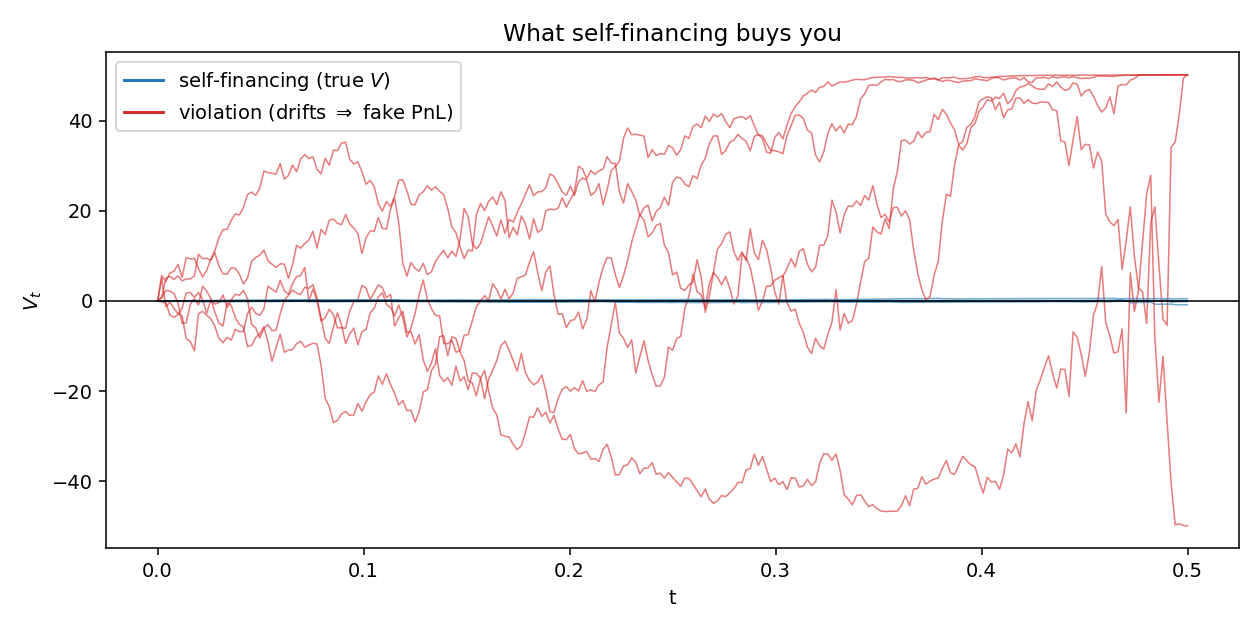
\includegraphics[keepaspectratio]{figures/ch06-self-financing-violation.png}}
\emph{Dropping the rebalance-cost term fabricates PnL --- the classic
``something for nothing'' that (6.8) forbids.}

\subsection{6.2.3 Applying the self-financing
constraint}\label{applying-the-self-financing-constraint}

After cancellation,

\[
\mathrm{d}V_t \;=\; \alpha_t\,\mathrm{d}g_t + \beta_t\,\mathrm{d}M_t - \mathrm{d}f_t. \tag{6.10}
\]

The only surviving terms are the three ``mark-to-market'' pieces: the
P\&L from the \(\alpha_t\) shares of \(g\) because \(g\) moved, the
interest accrual on the bank account, and the change in the liability
\(f\). There is \emph{nothing else}.

Substituting (6.2), (6.3), (6.5):

\[
\mathrm{d}V_t \;=\; \alpha_t\big(\mu^g_t g_t\,\mathrm{d}t + \sigma^g_t g_t\,\mathrm{d}W_t\big)
+ \beta_t M_t r_t\,\mathrm{d}t
- \big(\mu^f_t f_t\,\mathrm{d}t + \sigma^f_t f_t\,\mathrm{d}W_t\big). \tag{6.11}
\]

Collecting drift and diffusion,

\[
\boxed{\;\mathrm{d}V_t \;=\; \big(\alpha_t\mu^g_t g_t + \beta_t M_t r_t - \mu^f_t f_t\big)\,\mathrm{d}t
\;+\; \big(\alpha_t\sigma^g_t g_t - \sigma^f_t f_t\big)\,\mathrm{d}W_t\;} \tag{6.12}
\]

Equation (6.12) has the form
\(\mathrm{d}V_t = \text{drift}\,\mathrm{d}t +
\text{noise}\,\mathrm{d}W_t\), and we have two free knobs ---
\(\alpha_t\) and \(\beta_t\) --- to play with. The strategy is exactly
what a sensible trader would do in words: first get rid of the noise
(pick \(\alpha_t\) to annihilate the \(\mathrm{d}W_t\) coefficient),
then inspect what remains and let economics constrain the rest.

This two-stage procedure --- kill noise, then inspect drift --- is the
mathematical heart of every replication argument in finance. If the
underlying has \(k\) sources of risk instead of one, we need \(k\)
traded claims instead of one; we pick \(k\) holdings to kill each of the
\(k\) noise terms simultaneously; the remaining drift must equal the
risk-free rate on the net cash position. In the Heston
stochastic-volatility model, for example, there are two sources of risk
(the stock's diffusion and the volatility's diffusion), and we need two
hedge instruments (the stock and another option) to kill both.

\begin{center}\rule{0.5\linewidth}{0.5pt}\end{center}

\section{6.3 Locally removing the risk --- the delta-hedge
ratio}\label{locally-removing-the-risk-the-delta-hedge-ratio}

Locally remove risk, so set the \(\mathrm{d}W_t\) coefficient to zero:

\[
\alpha_t\,\sigma^g_t\,g_t - \sigma^f_t\,f_t \;=\; 0
\;\;\Longrightarrow\;\;
\boxed{\;\alpha_t \;=\; \frac{\sigma^f_t}{\sigma^g_t}\,\frac{f_t}{g_t}\;} \tag{6.13}
\]

This is the delta-hedge ratio in its most general form. Before we unpack
it, note what we have achieved: the instant we pick \(\alpha_t\) as
above, the \emph{random} part of \(\mathrm{d}V_t\) --- the bit that
depends on which direction the Brownian motion happened to move ---
disappears. Over a small enough interval, the portfolio is locally
riskless.

The formula has a crystalline interpretation: \(\alpha_t\) is the ratio
of the dollar-volatilities of \(f\) and \(g\). If \(f\) is twice as
volatile in dollar terms as \(g\), we need twice as many units of \(g\)
to keep up. In the common case where \(g = X\) (the stock itself is
traded), we have \(\sigma^g_t g_t = \sigma^x_t\) and
\(\sigma^f_t f_t = \sigma^x_t\,\partial_x
f\), so the ratio collapses to \(\alpha_t = \partial_x f\) --- the
partial derivative of the option value with respect to the spot, a.k.a.
the \emph{delta}. The replicating portfolio is the option's
Doppelgänger: at each instant, it holds exactly as much stock as the
option's price is sensitive to the stock --- no more, no less.

A concrete numerical illustration. Suppose the stock is trading at \$100
with \(\sigma = 20\%\), so the dollar volatility of one share is roughly
\(100 \cdot 0.20 = 20\) dollars per unit of \(W\). Suppose the option we
are hedging has \(\partial_x f = 0.6\), so its dollar volatility is
\(0.6 \cdot
20 = 12\) dollars per unit of \(W\). To neutralise the option's Brownian
motion exposure, we hold \(0.6\) shares of stock. If the stock now moves
by 1\% in a tiny interval, the option's price moves by
\(0.6 \cdot 1\% \cdot
100 = 0.60\) dollars and the share position moves by
\(0.6 \cdot 1 = 0.60\) dollars --- they cancel to the instant.

A useful edge case. A deep-ITM call has delta approaching 1, so the
hedger holds roughly one full share per option. A deep-OTM call has
delta approaching 0, so the hedger holds almost no stock, and the bank
account is approximately the option's premium invested at the risk-free
rate. Again, gamma is nearly zero, rebalancing is minimal. The hedging
problem is \emph{easy} in both extremes and hardest \emph{at the money},
where the delta is around 0.5 but the gamma is large and rebalancing is
frequent.

One subtlety worth flagging: the formula
\(\alpha_t = \partial_x f(t, X_t)\) is not a \emph{static} ratio. As
time passes and the stock moves, both arguments of the partial
derivative change, and the required hedge ratio changes too. This is why
dynamic hedging is called \emph{dynamic}: the hedge ratio is a moving
target that must be chased.

With this choice,

\[
\mathrm{d}V_t \;=\; \big(\alpha_t \mu^g_t g_t + \beta_t M_t r_t - \mu^f_t f_t\big)\,\mathrm{d}t
\;=\; \mathcal{A}_t\,\mathrm{d}t. \tag{6.14}
\]

After the \(\mathrm{d}W_t\) term has been killed, the remaining dynamics
are purely deterministic over an infinitesimal interval. The portfolio
earns some drift \(\mathcal{A}_t\) per unit time, and the question
becomes: what does that drift have to be?

\subsection{\texorpdfstring{6.3.1 No-arbitrage forces
\(\mathcal{A}_t = 0\)}{6.3.1 No-arbitrage forces \textbackslash mathcal\{A\}\_t = 0}}\label{no-arbitrage-forces-mathcala_t-0}

\begin{itemize}
\tightlist
\item
  If \(\mathcal{A}_t > 0\): profit guaranteed --- arbitrage.
\item
  If \(\mathcal{A}_t < 0\): reverse the strategy to get profit.
\end{itemize}

The argument is stark. We have built, by pure bookkeeping, a
self-financing portfolio with zero initial cost (\(V_0 = 0\)) and zero
instantaneous risk. If its value drifts upward, we are printing money;
if it drifts downward, we swap the signs of all holdings and \emph{then}
we are printing money. The only logical possibility consistent with no
free lunches is that the drift is exactly zero.

Therefore, to avoid arbitrage,

\[
\boxed{\;\mathcal{A}_t \;=\; 0\;}. \tag{6.15}
\]

Combined with \(V_0 = 0\), the entire portfolio process satisfies
\(V_t = 0\) for all \(t\), hence

\[
\mathcal{A}_t = 0 \;\Longrightarrow\; V_t = 0 \;\Longrightarrow\;
\alpha_t g_t + \beta_t M_t - f_t = 0
\;\Longrightarrow\; \beta_t M_t \;=\; f_t - \alpha_t g_t. \tag{6.16}
\]

(6.16) is the pricing identity. The unique cash holding that keeps the
hedge costless is \(f_t - \alpha_t g_t\) --- equivalently, the option's
value equals the value of the self-financing stock-plus-cash package
that replicates it.

Numerical: option \$3.50, delta 0.6, stock \$100. Hold 0.6 shares (\$60)
and borrow \$56.50; package value \(0.6 \cdot 100 - 56.50 = 3.50\).
Stock rises to \$101: shares worth \$60.60, option rises by
\(0.6 \cdot 1 = \$0.60\) to \$4.10. New delta 0.62 --- buy 0.02 shares,
fund via borrowing. Repeat every instant.

\begin{center}\rule{0.5\linewidth}{0.5pt}\end{center}

\section{6.4 Market price of risk}\label{market-price-of-risk}

Unpack the zero-drift consequence as a statement about expected returns.
Write out \(\mathcal{A}_t = 0\):

\[
\alpha_t \mu^g_t g_t + r_t\,(f_t - \alpha_t g_t) - \mu^f_t f_t \;=\; 0. \tag{6.17}
\]

Rearrange,

\[
\alpha_t\,\mu^g_t\,g_t + r_t f_t - r_t \alpha_t g_t - f_t \mu^f_t \;=\; 0. \tag{6.18}
\]

Recall \(\alpha_t = \dfrac{\sigma^f_t}{\sigma^g_t}\dfrac{f_t}{g_t}\).
Substituting and dividing by \(f_t\),

\[
\frac{\mu^g_t - r_t}{\sigma^g_t} \;=\; \frac{\mu^f_t - r_t}{\sigma^f_t}
\;=\; \lambda_t \;=\; \lambda(t,X_t). \tag{6.19}
\]

\begin{quote}
\textbf{Sharpe ratios of all assets on the underlying index are equal.}
\end{quote}

Every derivative on \(X\) --- call, digital, variance swap, structured
product --- has the same expected excess return per unit of volatility,
despite wildly different drifts and vols. \(\lambda_t\) is the
\textbf{market price of risk} --- a market property, not an
asset-specific quantity:

\[
\boxed{\;\frac{\mu^f_t - r_t}{\sigma^f_t} \;=\; \lambda_t
\;\Longleftrightarrow\;
\mu^f_t - r_t \;=\; \lambda_t\,\sigma^f_t\;}. \tag{6.20}
\]

\begin{quote}
\textbf{Connection to Girsanov.} Ch. 5 says: a Girsanov shift by
\(\lambda_t\) makes
\(\widetilde W_t = W_t + \int_0^t \lambda_s\,\mathrm{d}s\) a
\(\mathbb{Q}\)-Brownian motion, and \(X\)'s drift becomes
\(\mu^x_t - \sigma^x_t \lambda_t\). (6.20) picks out \emph{exactly} the
shift that neutralises the risk premium: under \(\mathbb{Q}\), every
traded claim drifts at \(r_t\). Market price of risk and Girsanov shift
are the same scalar.
\end{quote}

Rewriting (6.20) as \(\mu^f_t = r_t + \lambda_t \sigma^f_t\): expected
return = risk-free rate + vol \(\times\) price-per-unit-vol.~Under
\(\mathbb{Q}\) the risk premium is zero (the replicator sees no risk).
The shift is drift-only, leaving diffusion measure-invariant --- gamma
and vega P\&L are unchanged. Long-run US equity Sharpe of
\textasciitilde0.4 is the empirical \(\lambda\); spikes in crises.

\begin{center}\rule{0.5\linewidth}{0.5pt}\end{center}

\section{6.5 The generalised Black-Scholes
PDE}\label{the-generalised-black-scholes-pde}

The scalar identity \(\mu^f - r = \lambda \sigma^f\) becomes a PDE once
we substitute the Itô expressions for \(\mu^f\) and \(\sigma^f\) in
terms of partial derivatives of \(f(t, x)\). Via Itô's lemma:

\[
\mu^f_t \;=\; \frac{\partial_t f_t + \mu^x_t\,\partial_x f_t
+ \tfrac{1}{2}(\sigma^x_t)^2\,\partial_{xx}f_t}{f_t}, \tag{6.21}
\]

\[
\sigma^f_t \;=\; \frac{\sigma^x_t\,\partial_x f_t}{f_t}. \tag{6.22}
\]

(Here \(\mu^x_t,\sigma^x_t\) are the coefficients of \(X\) from (6.1).)
Plug into \(\mu^f_t - r_t = \lambda_t \sigma^f_t\):

\[
\partial_t f_t + \big(\mu^x_t - \sigma^x_t \lambda_t\big)\,\partial_x f_t
+ \tfrac{1}{2}(\sigma^x_t)^2\,\partial_{xx}f_t \;=\; r_t\,f_t. \tag{6.23}
\]

This has to hold \(\forall (t,x)\). Hence:

\[
\boxed{\;\begin{aligned}
&\partial_t f(t,x) + \big(\mu^x(t,x) - \sigma^x(t,x)\,\lambda(t,x)\big)\,\partial_x f(t,x) \\
&\qquad + \tfrac{1}{2}\big(\sigma^x(t,x)\big)^2\,\partial_{xx}f(t,x) \;=\; r(t,x)\,f(t,x), \\
&\qquad\qquad\qquad\qquad\qquad f(T,x) \;=\; \varphi(x).
\end{aligned}\;} \tag{6.24}
\]

\textbf{Generalised Black-Scholes PDE.} Backwards parabolic; the
terminal \(f(T, x) = \varphi(x)\) anchors the payoff shape and the PDE
propagates it back. Sharp features (kinks, steps, cliffs) smooth out as
time runs backward --- diffusion smearing.

The drift coefficient \(\mu^x - \sigma^x \lambda\) is the
\emph{risk-neutral} drift, not the physical one --- exactly the Girsanov
shift (Ch. 5). The \(\tfrac12 (\sigma^x)^2 \partial_{xx} f\) term is the
Itô curvature, independent of drift --- which is why option prices do
not depend on \(\mu\). The RHS \(r f\) says the replicator grows at the
risk-free rate.

\begin{quote}
\textbf{What happens when \(\Delta\) is wrong.} If
\(\alpha_t \neq \partial_x f\), the \(\mathrm{d}W_t\) coefficient is
non-zero. Hedge error over \([t, t+\mathrm{d}t]\) is
\((\alpha_t \sigma^g_t g_t - \sigma^f_t f_t)\,\mathrm{d}W_t\) ---
mean-zero noise plus a second-order
\(\tfrac12 \partial_{xx} f (\mathrm{d}X_t^2 - \sigma^2 X_t^2 \mathrm{d}t)\)
that accumulates as realised-minus-implied variance. This is the
\textbf{P\&L attribution}: discretely-hedged short gamma loses money
when realised vol exceeds implied. See \texttt{ch06-hedge-error.png}.
\end{quote}

Equivalently, an option is a position in variance: instantaneous P\&L is
\(\tfrac12 \Gamma S^2 (\sigma_{\text{imp}}^2 - \sigma_{\text{real}}^2)\,\mathrm dt\).
The PDE is linear in \(f\), so portfolio prices are sums of individual
prices.

\pandocbounded{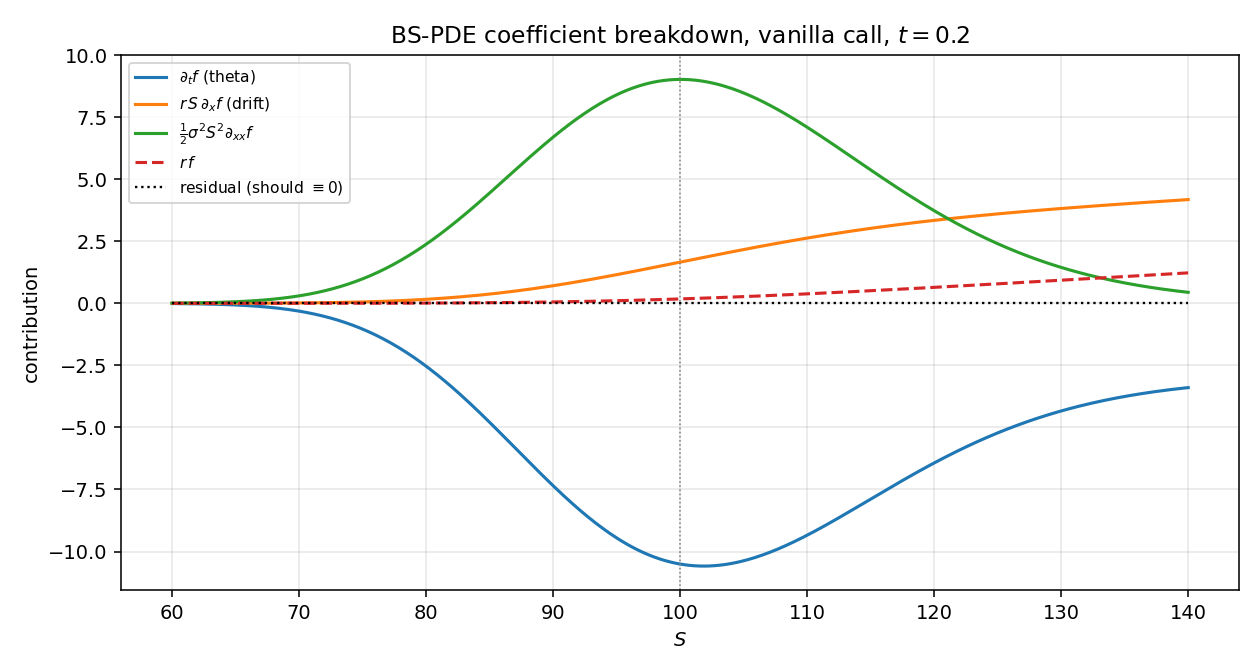
\includegraphics[keepaspectratio]{figures/ch06-pde-coefficients.png}}
\emph{Theta pays for gamma: the three LHS terms balance \(r f\) exactly
--- the dotted residual is numerically zero.}

\begin{center}\rule{0.5\linewidth}{0.5pt}\end{center}

\section{6.6 Specialising to Black-Scholes
(GBM)}\label{specialising-to-black-scholes-gbm}

Specialise to GBM, where the stock has constant proportional drift and
vol and is traded directly (\(g = X\)):

\[
\mu^x(t,x) \;=\; \mu x, \qquad \sigma^x(t,x) \;=\; \sigma x,
\]

so

\[
\mathrm{d}X_t \;=\; X_t \mu\,\mathrm{d}t + X_t \sigma\,\mathrm{d}W_t. \tag{6.25}
\]

In divided form,
\(\mathrm{d}S_t/S_t = \mu\,\mathrm{d}t + \sigma\,\mathrm{d}W_t\). Itô on
\(\ln S_t\) gives

\[
\mathrm{d}(\ln S_t) \;=\; \big(\mu - \tfrac12\sigma^2\big)\,\mathrm{d}t \;+\; \sigma\,\mathrm{d}W_t,
\]

which integrates immediately. Exponentiating,

\[
S_t \;=\; S_0\,\exp\!\Big(\big(\mu - \tfrac12\sigma^2\big)\,t \;+\; \sigma W_t\Big)
\;\stackrel{d}{=}\; S_0\,\exp\!\Big(\big(\mu - \tfrac12\sigma^2\big)\,t \;+\; \sigma\sqrt{t}\,Z\Big),
\qquad Z \sim \mathcal{N}(0,1).
\tag{6.25a}
\]

\(S_t\) is log-normal with log-mean \((\mu - \tfrac12\sigma^2)t\) and
log-variance \(\sigma^2 t\). The \(-\tfrac12\sigma^2\) Itô correction is
what makes \(\mathbb{E}[S_t] = S_0 e^{\mu t}\) exactly.

With \(g(t, x) = x\) (\(\sigma^g = \sigma\), \(\mu^g = \mu\)) and
constant \(r\),

\[
\lambda \;=\; \frac{\mu - r}{\sigma}. \tag{6.26}
\]

In GBM, \(\lambda\) is literally the stock's Sharpe ratio --- the origin
of the name and the motivation for \(\mathbb{Q}\) as the measure under
which the stock drifts at \(r\). Substituting into (6.24):

\[
\partial_t f + \underbrace{(\mu - \sigma\lambda)}_{=\,r}\,x\,\partial_x f
+ \tfrac{1}{2}\sigma^2 x^2\,\partial_{xx}f \;=\; r f.
\]

\[
\boxed{\;\begin{aligned}
&\partial_t f + r\,x\,\partial_x f + \tfrac{1}{2}\sigma^2 x^2\,\partial_{xx} f \;=\; r f, \\
&f(T,x) \;=\; \varphi(x).
\end{aligned}\;} \tag{6.27}
\]

\textbf{Black-Scholes PDE.} The stock's physical drift \(\mu\) has
disappeared completely --- absorbed by \(\mu - \sigma\lambda = r\). Two
stocks with the same \(\sigma\) but different \(\mu\) produce identical
call prices because the hedger replicates state-by-state regardless of
drift; cost depends on how hard the replication machine has to work
(vol), not on direction. Implied volatility is then the market's
\(\mathbb{Q}\)-measure forecast of root-mean-square log-returns; for
liquid equity options the gap to the \(\mathbb{P}\)-forecast is small.

\begin{center}\rule{0.5\linewidth}{0.5pt}\end{center}

\section{6.7 Black-Scholes formulas for call, put, and
digital}\label{black-scholes-formulas-for-call-put-and-digital}

The closed forms follow from (6.27) by ansatz, by direct
\(\mathbb{Q}\)-expectation under (6.25a), or via Feynman--Kac (Ch. 4).
Derivation in §6.7A.

\textbf{Vanilla call.} For \(\varphi(x) = (x - K)_+\),

\[
\boxed{\;f(t,x) \;=\; x\,\Phi(d_+) \;-\; K\,e^{-r(T-t)}\,\Phi(d_-)\;} \tag{6.28}
\]

with

\[
d_\pm \;=\; \frac{\ln(x/K) + \big(r \pm \tfrac{1}{2}\sigma^2\big)(T-t)}{\sigma\sqrt{T-t}}. \tag{6.29}
\]

\textbf{Black--Scholes call.} Two pieces: \(x\Phi(d_+)\) is the expected
stock payoff conditional on ITM expiry (under the stock-numeraire
measure); \(Ke^{-r(T-t)}\Phi(d_-)\) is the discounted strike times the
\(\mathbb{Q}\)-probability of ITM expiry. The symmetry
\(d_+ = d_- + \sigma\sqrt{T-t}\) is the ``vol lift'' --- conditional on
finishing ITM the expected log-price sits above its unconditional
median.

\textbf{Vanilla put} via put-call parity. From
\((X_T - K)_+ - (K - X_T)_+ = X_T - K\):

\[
\boxed{\;C(t,x) - P(t,x) \;=\; x - K\,e^{-r(T-t)}\;} \tag{6.30}
\]

Parity is \textbf{model-independent}: it follows from the algebraic
identity plus existence of \(\mathbb{Q}\). Violations are the cleanest
arbitrage signal. Solving for \(P\):

\[
\boxed{\;P(t,x) \;=\; K\,e^{-r(T-t)}\,\Phi(-d_-) \;-\; x\,\Phi(-d_+)\;} \tag{6.31}
\]

\textbf{Digital call.} For \(\varphi(x) = \mathbb{1}_{x \ge K}\), the
price is the discounted \(\mathbb{Q}\)-ITM probability:

\[
\boxed{\;f(t,x) \;=\; e^{-r(T-t)}\,\Phi(d_-)\;} \tag{6.32}
\]

since \(\{X_T \ge K\} = \{Z \ge -d_-\}\) under GBM.

\subsection{6.7.1 Greeks from the closed
form}\label{greeks-from-the-closed-form}

The \textbf{strike-shifting identity}
\(x\phi(d_+) = Ke^{-r(T-t)}\phi(d_-)\) collapses the algebra:

\begin{itemize}
\tightlist
\item
  \textbf{Delta}:
  \(\Delta^C \;=\; \partial_x f \;=\; \Phi(d_+) \in (0,1)\).
\item
  \textbf{Gamma}:
  \(\Gamma^C \;=\; \partial_{xx} f \;=\; \dfrac{\phi(d_+)}{x\,\sigma\sqrt{T-t}}\).
\item
  \textbf{Vega}:
  \(\mathcal{V}^C \;=\; \partial_\sigma f \;=\; x\,\phi(d_+)\,\sqrt{T-t}\).
\end{itemize}

For the put, parity gives \(\Delta^P = \Delta^C - 1 \in (-1, 0)\) and
\(\Gamma^P = \Gamma^C\) (differentiating parity twice in \(x\)): calls
and puts of the same strike and maturity have \emph{identical} gamma.
Vega is also shared: \(\mathcal{V}^P = \mathcal{V}^C\).

The gamma formula exhibits a striking \(1/\sqrt{T-t}\) divergence at the
money as \(t \to T\): the at-the-money gamma blows up like
\(1/\sqrt{T-t}\). This is the \emph{pin gamma} phenomenon --- on
expiration day a market-maker's gamma exposure is effectively all in a
narrow band around the strike, which is why gamma books are rebalanced
with extra care on expiration Fridays. Integrated across spot, however,
\(\int \Gamma^C\,\mathrm{d}x =
\Delta^C(\infty) - \Delta^C(0) = 1 - 0 = 1\): the total gamma ``mass''
is conserved across time-to-expiry. What changes is how that mass is
distributed spatially.

\textbf{Digital greeks.} The digital call's delta from (6.32) is

\[
\partial_x f^{\mathrm{dig}} \;=\; e^{-r(T-t)}\,\frac{\phi(d_-)}{x\,\sigma\sqrt{T-t}},
\tag{6.33}
\]

which has a \emph{pathological} limit as \(T - t \to 0\) at \(x = K\):
the numerator \(\phi(d_-) \to \phi(0) = 1/\sqrt{2\pi}\) is bounded away
from zero, while the denominator \(\sqrt{T-t}\) tends to zero. The delta
blows up without bound at the strike. We will visualise this in §6.11.7
and discuss the call-spread hedge that practitioners use to tame it.

\pandocbounded{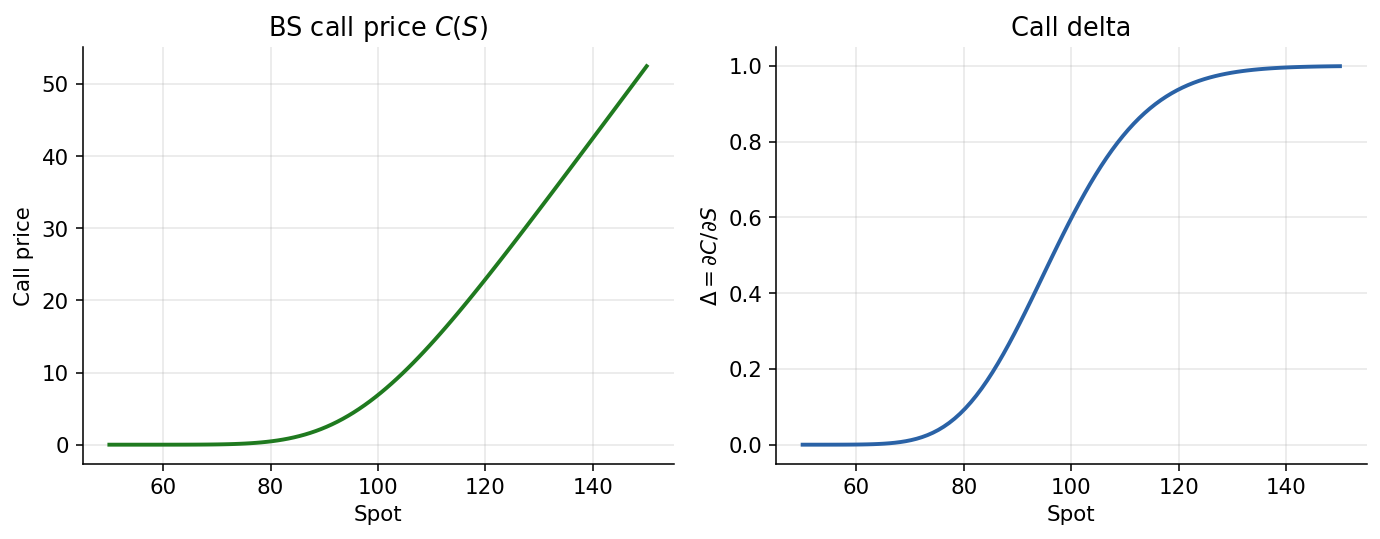
\includegraphics[keepaspectratio]{figures/ch06-price-delta.png}}
\emph{BS price and delta curves.}

\begin{center}\rule{0.5\linewidth}{0.5pt}\end{center}

\section{6.7A Dual derivation via
Feynman-Kac}\label{a-dual-derivation-via-feynman-kac}

The self-financing hedging argument of §§6.2--6.5 is the route by which
Black, Scholes, and Merton originally derived the PDE (6.27). There is a
second, entirely independent route that arrives at \emph{exactly} the
same PDE and the same formulas: the \textbf{Feynman-Kac} bridge of
Chapter 4. Seeing both routes is worthwhile because they foreground
different pieces of the machinery and their agreement is the mark of a
solid theory.

\subsection{6.7A.1 Setup under the risk-neutral
measure}\label{a.1-setup-under-the-risk-neutral-measure}

Under the risk-neutral measure \(\mathbb{Q}\) constructed in Chapter 5,
the traded asset and bank account satisfy

\[
\frac{\mathrm{d}S_t}{S_t} \;=\; r\,\mathrm{d}t \;+\; \sigma\,\mathrm{d}\widetilde W_t, \qquad
\frac{\mathrm{d}M_t}{M_t} \;=\; r\,\mathrm{d}t, \tag{6.34}
\]

where \(\widetilde W_t\) is a \(\mathbb{Q}\)-Brownian motion. The drift
is \(r\), not the real-world \(\mu\), because \(\mathbb{Q}\) is chosen
so that \(S_t/M_t\) is a \(\mathbb{Q}\)-martingale --- and that
martingale condition forces the drift of \(\mathrm{d}S/S\) to equal
\(r\). The physical expected return \(\mu\) never appears in derivative
prices; it is \emph{absorbed into the measure change} via the
Radon-Nikodym derivative of Chapter 5, with Girsanov shift
\(\lambda = (\mu - r)/\sigma\).

\subsection{6.7A.2 Applying Feynman-Kac}\label{a.2-applying-feynman-kac}

The claim \(\xi = (\xi_t)\) with \(\xi_T = \varphi(S_T)\) has pricing
function \(F_t = f(t, S_t)\). Feynman-Kac (Chapter 4) applied with drift
\(a(x) = rx\), diffusion \(b(x) = \sigma x\), and discounting \(c = r\)
yields the representation

\[
f(t, x) \;=\; \mathbb{E}_{t,x}^{\mathbb{Q}}\!\left[\,e^{-r(T-t)}\,\varphi(X_T)\,\right],
\qquad \mathrm{d}X_s = r\,X_s\,\mathrm{d}s + \sigma\,X_s\,\mathrm{d}\widetilde W_s.
\tag{6.35}
\]

By the Chapter 4 FK theorem, \(f(t,x)\) satisfies the PDE

\[
\partial_t f + r\,x\,\partial_x f + \tfrac12\sigma^2 x^2\,\partial_{xx} f \;=\; r\,f, \qquad f(T,x) = \varphi(x).
\tag{6.36}
\]

This is \emph{identical} to (6.27). Two independent derivations --- the
hedging argument of §6.5 and the FK martingale argument of Chapter 4 ---
converge on the same PDE. That convergence is not a coincidence; both
are expressing the same fact in different languages.

\subsection{\texorpdfstring{6.7A.3 Discounted price as a
\(\mathbb{Q}\)-martingale}{6.7A.3 Discounted price as a \textbackslash mathbb\{Q\}-martingale}}\label{a.3-discounted-price-as-a-mathbbq-martingale}

The clearest way to see the equivalence is via the discounted price. Let
\(Y_t := f(t, X_t)/M_t\). Applying Itô's lemma (Chapter 3) and
collecting the \(\mathrm{d}t\) terms gives

\[
\mathrm{d}Y_t \;=\; \frac{1}{M_t}\!\left(\partial_t f + r x\,\partial_x f + \tfrac12\sigma^2 x^2 \partial_{xx} f - r f\right)\!\mathrm{d}t \;+\; \frac{\sigma x \,\partial_x f}{M_t}\,\mathrm{d}\widetilde W_t.
\tag{6.37}
\]

By the Black-Scholes PDE (6.36), the \(\mathrm{d}t\) bracket vanishes
identically, leaving only the Brownian piece --- i.e.~\(Y\) is a (local)
martingale. \textbf{The PDE is exactly the drift-killer}: \(\mathbb{Q}\)
is defined so the bracket equals zero.

The BS PDE is ``discounted price is a \(\mathbb{Q}\)-martingale'' in Itô
language.

\begin{quote}
\textbf{Martingale \(\;\Leftrightarrow\;\) drift is zero
\(\;\Leftrightarrow\;\) PDE holds.}
\end{quote}

\subsection{6.7A.4 Recovering the call formula from the
expectation}\label{a.4-recovering-the-call-formula-from-the-expectation}

Integrate
\(\mathrm{d}X_s/X_s = r\,\mathrm{d}s + \sigma\,\mathrm{d}\widetilde W_s\)
from \(X_t = x\):

\[
X_T \;=\; x\cdot\exp\!\Big\{(r - \tfrac12\sigma^2)(T - t) + \sigma(\widetilde W_T - \widetilde W_t)\Big\}. \tag{6.38}
\]

Decompose the call payoff as \((X_T - K)_+ = X_T\,\mathbb{1}_{X_T > K} -
K\,\mathbb{1}_{X_T > K}\). The second piece is the discounted digital
times \(K\): from (6.32), \(K\,e^{-r(T-t)}\,\Phi(d_-)\). The first piece
--- the stock-delivery leg --- uses the change-of-numeraire trick of
Chapter 5. Under the stock-numeraire measure \(\mathbb{Q}^S\) (with
\(S_t\) as numeraire rather than the money account \(M_t\)), the
expectation \(\mathbb{E}^{\mathbb{Q}^S}[\mathbb{1}_{X_T >
K}]\) equals \(\Phi(d_+)\) with \(d_+ = d_- + \sigma\sqrt{T-t}\).
Translating back to the \(\mathbb{Q}\)-expectation via the Radon-Nikodym
density
\(\mathrm{d}\mathbb{Q}^S/\mathrm{d}\mathbb{Q} = S_T/(S_t\,e^{r(T-t)})\):

\[
\mathbb{E}_{t,x}^{\mathbb{Q}}\!\left[e^{-r(T-t)}\,X_T\,\mathbb{1}_{X_T > K}\right] \;=\; x\cdot\Phi(d_+). \tag{6.39}
\]

Combining the two pieces recovers (6.28).
\(\Phi(d_-) = \mathbb{Q}(X_T > K)\) is the risk-neutral exercise
probability; \(\Phi(d_+) = \mathbb{Q}^S(X_T > K)\) is the same under the
stock numeraire --- they differ by the Girsanov shift
\(\sigma\sqrt{T-t}\).

\subsection{6.7A.5 Why two derivations}\label{a.5-why-two-derivations}

Hedging foregrounds self-financing, market price of risk, no-arbitrage.
Feynman--Kac foregrounds the measure change: the PDE is the drift-killer
that defines \(\mathbb{Q}\). For Gaussian-integrable payoffs (calls,
digitals, log-contracts), the expectation route wins; for
low-dimensional non-integrable problems with American or barrier
features, the PDE route via finite differences wins.

\begin{center}\rule{0.5\linewidth}{0.5pt}\end{center}

\section{\texorpdfstring{6.8 Worked Example 1 --- Linear payoff
\(\varphi(x) = x\) (sanity
check)}{6.8 Worked Example 1 --- Linear payoff \textbackslash varphi(x) = x (sanity check)}}\label{worked-example-1-linear-payoff-varphix-x-sanity-check}

The claim that pays the stock price at maturity must price at
\(f(t, x) = x\). PDE check:

\[
\partial_t f = 0,\qquad \partial_x f = 1,\qquad \partial_{xx} f = 0,
\]

so the LHS of (6.27) is \(0 + rx\cdot 1 + 0 = rx = r f\). ✓

Delta is 1 --- replicate by holding one share, no cash. A useful smoke
test for any FD scheme.

\textbf{Probabilistic.} Under \(\mathbb{Q}\),

\[
X_T \;\overset{d}{=}\; X_t\,e^{(r - \tfrac{1}{2}\sigma^2)(T-t) + \sigma\sqrt{T-t}\,Z},
\qquad Z \sim \mathcal{N}(0,1).
\]

Hence

\[
\text{price} \;=\; \mathbb{E}^{\mathbb{Q}}_t\!\left[e^{-r(T-t)}\,X_T\right]
\;=\; X_t\,\mathbb{E}^{\mathbb{Q}}\!\left[e^{-\tfrac{1}{2}\sigma^2(T-t) + \sigma\sqrt{T-t}\,Z}\right] \;=\; X_t. \tag{6.40}
\]

The bracket is a mean-1 log-normal --- Feynman--Kac agrees with the PDE.

\begin{center}\rule{0.5\linewidth}{0.5pt}\end{center}

\section{\texorpdfstring{6.9 Worked Example 2 --- Separable ansatz
\(f(t, x) = x^2\,\ell(t)\)}{6.9 Worked Example 2 --- Separable ansatz f(t, x) = x\^{}2\textbackslash,\textbackslash ell(t)}}\label{worked-example-2-separable-ansatz-ft-x-x2ellt}

The squared payoff \(\varphi(x) = x^2\) is a building block of variance
swaps and log-contract decompositions, and the simplest non-linear
payoff in the Itô world. Ansatz \(f(t, x) = x^2 \ell(t)\) with
\(\ell(T) = 1\):

\[
\partial_t f = x^2\,\dot\ell,\qquad \partial_x f = 2 x \ell,\qquad \partial_{xx} f = 2\ell.
\]

Plug into (6.27):

\[
\underbrace{x^2\dot\ell}_{\partial_t f}
+ \underbrace{rx\cdot 2x\ell}_{rx\,\partial_x f}
+ \underbrace{\tfrac{1}{2}\sigma^2 x^2\cdot 2\ell}_{\tfrac{1}{2}\sigma^2 x^2\,\partial_{xx}f}
\;=\; \underbrace{r\,x^2\ell}_{rf}. \tag{6.41}
\]

Divide by \(x^2\):

\[
\dot\ell + (r + \sigma^2)\ell \;=\; 0
\;\Longrightarrow\;
\ell(t) \;=\; e^{(r + \sigma^2)(T - t)}. \tag{6.42}
\]

So

\[
\boxed{\;f(t,x) \;=\; x^2\,e^{(r+\sigma^2)(T-t)}\;}. \tag{6.43}
\]

Volatility shows up additively to the rate in the exponent --- variance
products are exponential in \(\sigma^2\) and so deeply vega-heavy. The
ansatz collapses a 2-variable PDE to a 1-variable ODE; this trick works
for any power-of-\(x\) payoff.

Delta \(= 2 x \ell(t)\), gamma \(= 2 \ell(t)\) (constant). Constant
gamma is the cleanest vehicle for harvesting realised variance --- the
basis of variance-swap replication via the log-contract decomposition.

Numeric: \(r = 5\%\), \(\sigma = 20\%\), \(T - t = 1\) gives
\(e^{0.09} \approx 1.094\) --- a 9.4\% premium over the cash-and-carry
square. Shock \(\sigma\) to 30\% and the premium is 15\%.

\begin{center}\rule{0.5\linewidth}{0.5pt}\end{center}

\section{6.9A Worked Example 3 --- Digital call (closed form + PDE
verification)}\label{a-worked-example-3-digital-call-closed-form-pde-verification}

A digital pays \$1 if \(S_T \ge K\). The pricing formula is clean
((6.32)), but the discontinuity makes hedging near expiry pathological
--- see §6.11.7.

\textbf{Payoff and closed form.} Recall

\[
\varphi(x) \;=\; \mathbb{1}_{\,x \,\ge\, K}, \qquad
f(t,x) \;=\; e^{-r(T-t)}\,\Phi\!\big(d_-(t,x)\big), \tag{6.44}
\]

with

\[
d_-(t,x) \;=\; \frac{\ln(x/K) + (r - \tfrac{1}{2}\sigma^2)(T-t)}{\sigma\sqrt{T-t}}. \tag{6.45}
\]

Numeric: \(S = K = \$100\), \(r = 5\%\), \(\sigma = 20\%\),
\(T - t = 0.5\). Then \(d_- = 0.015 / 0.1414 \approx 0.106\),
\(\Phi(0.106) \approx 0.542\), and the price is
\(e^{-0.025} \cdot 0.542 \approx 0.529\) --- 53 cents per dollar at
expiry.

\subsection{6.9A.1 PDE verification}\label{a.1-pde-verification}

Chain-rule the partials of \(\Phi(d_-(t, x))\):

\[
\partial_t f \;=\; e^{-r(T-t)}\,\Phi'(d_-(t,x))\,\partial_t d_-
\;+\; r\,f. \tag{6.46}
\]

Space derivatives:

\[
\partial_x f \;=\; e^{-r(T-t)}\,\Phi'(d_-(t,x))\,\partial_x d_-,
\qquad \partial_x d_- \;=\; \frac{1}{x\,\sigma\sqrt{T-t}}, \tag{6.47}
\]

\[
\partial_{xx} f \;=\; e^{-r(T-t)}\Big\{\Phi''(d_-(t,x))\,(\partial_x d_-)^2 + \Phi'(d_-(t,x))\,\partial_{xx} d_-\Big\}, \tag{6.48}
\]

with

\[
\partial_{xx} d_- \;=\; -\,\frac{1}{x^2\,\sigma\sqrt{T-t}},
\qquad \Phi''(x) \;=\; -\,x\,\Phi'(x),\quad \Phi'(x) \;=\; \frac{e^{-\tfrac{1}{2}x^2}}{\sqrt{2\pi}}. \tag{6.49}
\]

Combining (6.46)-(6.49) in (6.27) verifies the PDE: the \(rf\) terms
cancel against \(\partial_t f\)'s \(+rf\) piece, and the
drift-plus-diffusion piece cancels thanks to \(\Phi'' = -x\Phi'\). ✓

The identity \(\Phi'' = -x\Phi'\) collapses the cross-terms at the right
moment.

The digital's delta is
\(\partial_x f = e^{-r(T-t)} \Phi'(d_-) / (x \sigma \sqrt{T-t})\).
Off-strike, \(d_- \to \pm\infty\) kills \(\Phi'(d_-)\) exponentially as
\(T - t \to 0\). At-strike, \(\Phi'(d_-)\) stays bounded and the delta
is dominated by the \(1/\sqrt{T-t}\) singularity --- ``infinite delta at
the strike in the last instant'' (visualised in §6.11.7).

For \(K = \$100\), \(\sigma = 20\%\): peak delta is
\(\approx 0.07\)/dollar at 1 month, \(\approx 0.4\)/dollar at 1 day,
\(\approx 2\)/dollar at 1 hour --- untradeable. Digital hedging is a
race against the clock.

\begin{center}\rule{0.5\linewidth}{0.5pt}\end{center}

\section{6.10 Time-based hedging
recursion}\label{time-based-hedging-recursion}

Any PDE solution rewrites as a discounted \(\mathbb{Q}\)-expectation by
Feynman--Kac. Replication, PDE, and expectation are three statements of
the same no-arbitrage fact. Under \(\mathbb{Q}\),

\[
f(t,x) \;=\; \mathbb{E}^{\mathbb{Q}}_{t,x}\!\left[\varphi(X_T)\,e^{-\int_t^T r_u\,\mathrm{d}u}\right], \qquad X_t = x. \tag{6.50}
\]

Under \(\mathbb{Q}\) the drift of \(X\) is shifted by
\(-\sigma^x \lambda\) --- in BS this collapses to \(r X_t\). The
physical \(\mu\) is entirely absent from the pricing machine. The
\(\mathbb{Q}\)-dynamics:

\[
\mathrm{d}X_t \;=\; \underbrace{\big(\mu^x_t - \sigma^x_t\,\lambda_t\big)}_{\,=\,r_t X_t\text{ in BS}}\,\mathrm{d}t
\;+\; \sigma^x_t\,\mathrm{d}\widetilde W_t, \tag{6.51}
\]

where \(\widetilde W_t\) is \(\mathbb{Q}\)-Brownian. Under
\(\mathbb{Q}\), every discounted traded price is a martingale --- which
is why (6.50) works.

The \textbf{Fundamental Theorem of Asset Pricing} formalises this
connection. It states that, in a market satisfying mild technical
conditions, there is no arbitrage if and only if there exists at least
one equivalent martingale measure \(\mathbb{Q}\) under which all
discounted traded prices are martingales. Furthermore, if the market is
complete (as in our single-Brownian-motion setup), the martingale
measure is unique. Self- financing plus no-arbitrage implies the
existence of \(\mathbb{Q}\); market completeness implies uniqueness; and
the risk-neutral expectation (6.50) is what you get when you integrate
any payoff against this unique measure.

\subsection{6.10.1 Specialisation to
Black-Scholes}\label{specialisation-to-black-scholes}

\[
\mathrm{d}X_t \;=\; \mu X_t\,\mathrm{d}t + \sigma X_t\,\mathrm{d}W_t
\;=\; r\,X_t\,\mathrm{d}t + \sigma X_t\,\mathrm{d}\widetilde W_t,\qquad r = \text{const}. \tag{6.52}
\]

The call, put, and digital formulas (6.28), (6.31), and (6.32) all
follow from plugging (6.38) into (6.50) and computing the Gaussian
integrals, as sketched in §6.7A.4. The three formulas are the three
canonical closed forms that every option-pricing library implements.

It is worth writing out what the Greeks mean in units. The delta
\(\Phi(d_+)\) is dimensionless --- it is the number of shares per
option. The gamma \(\phi(d_+)/(x\sigma\sqrt{T-t})\) has units of shares
per dollar of stock, which is to say ``how fast the delta changes as the
stock moves''. The vega \(x\phi(d_+)\sqrt{T-t}\) has units of dollars
per unit of volatility; a typical convention is to quote vega per ``vol
point'' (1\% change in \(\sigma\)), which gives the dollar sensitivity
of the option to a one-percentage-point move in implied volatility.
These three numbers are the core risk measures of the option position;
any serious trading desk watches them in real time.

The curvature features of the vanilla call are specially illuminating.
The gamma peaks at-the-money because that is where the payoff has its
``kink''; further from the strike, the payoff is either essentially
linear (deep ITM) or essentially zero (deep OTM), and a linear payoff
has no curvature. The gamma also grows as expiry approaches for
at-the-money options, because the remaining convexity has to be
concentrated into a shrinking window. Gamma and vega are cousins ---
both express the option's exposure to variance --- and they are most
pronounced where the payoff is most non-linear.

\begin{center}\rule{0.5\linewidth}{0.5pt}\end{center}

\section{6.11 Discrete hedging of a continuous
model}\label{discrete-hedging-of-a-continuous-model}

The theoretical result is that continuous rebalancing at every instant
produces \emph{exact} replication --- \(V_t \equiv 0\), every day, every
path. In real life, we rebalance at some discrete frequency: daily,
hourly, once per tick. The replication therefore has tracking error, and
the structure of that error is what we turn to now. We will see that the
dominant source of error scales like \(\sqrt{\Delta t}\) per step, and
that --- importantly --- this error comes from discretisation of the
Brownian motion, not from any model mismatch. Model mismatch is a
separate, more insidious source of error.

The transition from the continuous-time theory to real-world hedging is
where the rubber meets the road. On paper, continuous rebalancing
produces exact replication; in reality, the fastest any trader can
rebalance is tick-by-tick, and even tick-by-tick is at millisecond
intervals, not truly continuous. The gap between ``continuous'' and
``very frequently'' is not just a quantitative small-error question ---
it has a specific structure that shapes how traders set up their
rebalancing workflows.

\subsection{6.11.1 Holdings rule}\label{holdings-rule}

\[
\alpha_t \;=\; \frac{\sigma^f_t\,f_t}{\sigma^g_t\,g_t}
\;=\; \partial_x f(t,X_t)\qquad \text{if } X_t \text{ is traded.} \tag{6.53}
\]

The stock-hedge ratio is the delta --- hence ``delta hedging.'' In
practice we hold \(\partial_x f\) at the last rebalance and let the
position drift. Two error sources: path-dependent (stock moves between
rebalances, ideal delta shifts) and calendar-dependent (\(\partial_x f\)
depends on \(t\)). Geometrically, between trades the held portfolio is
an affine tangent to the curved pricing surface; the curvature gap is
the gamma residual.

\subsection{\texorpdfstring{6.11.2 At \(t_0 = 0\) --- sold \(f\), get
\(f_0\)}{6.11.2 At t\_0 = 0 --- sold f, get f\_0}}\label{at-t_0-0-sold-f-get-f_0}

\begin{itemize}
\tightlist
\item
  Buy \(\alpha_0\) units of \(X\) (costs \(\alpha_0 X_0\)).
\item
  Bank: \(M_0 = f_0 - \alpha_0 X_0\).
\end{itemize}

Numerical: 3-month ATM call on \$100 stock, 25\% vol, 5\% rate. Premium
\(\approx \$5.60\), delta \(\approx 0.55\). Buy 0.55 shares for \$55,
bank starts at \(-\$49.40\) --- short calls require borrowing to fund
the hedge.

\subsection{\texorpdfstring{6.11.3 At
\(t_1\)}{6.11.3 At t\_1}}\label{at-t_1}

Bank grew at interest, then we rebalance to the new delta:

\[
M_{t_1} \;=\; M_0\,e^{r\,\Delta t} \;-\; (\alpha_{t_1} - \alpha_{t_0})\,X_{t_1}. \tag{6.54}
\]

The rebalance price is the current \(X_{t_1}\), not the old one --- that
is what self-financing enforces vs the naive product rule.

\subsection{\texorpdfstring{6.11.4 At
\(t_2\)}{6.11.4 At t\_2}}\label{at-t_2}

\[
M_{t_2} \;=\; M_{t_1}\,e^{r\,\Delta t} \;-\; (\alpha_{t_2} - \alpha_{t_1})\,X_{t_2}. \tag{6.55}
\]

\subsection{6.11.5 Repeat}\label{repeat}

\[
\boxed{\;M_{t_n} \;=\; M_{t_{n-1}}\,e^{r\,\Delta t} \;-\; (\alpha_{t_n} - \alpha_{t_{n-1}})\,X_{t_n}\;} \tag{6.56}
\]

No rebalancing between \(t_0, t_1, \dots, t_N = T\).

With per-trade transaction cost \(\kappa(q)\) on \(q\) shares,

\[
M_k \;=\; M_{k-1}\,e^{r\,\Delta t_k} \;-\; (\alpha_k - \alpha_{k-1})\,S_k \;-\; \kappa\!\big(\alpha_k - \alpha_{k-1}\big), \tag{6.57}
\]

and \(\sum_k \kappa(\Delta\alpha_k)\) is the slippage bill that turns
rebalancing into a genuine optimisation rather than ``rebalance as often
as possible.''

\subsection{6.11.6 Terminal P\&L}\label{terminal-pl}

At \(t_N\) we owe the option payoff:

\[
\boxed{\;\mathrm{PnL} \;=\; \Big(M_{t_{N-1}}\,e^{r\,\Delta t} \;+\; \alpha_{t_{N-1}}\,X_{t_N}\Big) \;-\; \varphi(X_{t_N})\;} \tag{6.58}
\]

Exact replication would give PnL \(\equiv 0\). In reality, two distinct
error sources contribute.

\textbf{Discretisation error} (\(\sqrt{\Delta t}\) scaling, vanishes as
\(\Delta t \to 0\)). On each step the residual mismatch between the held
constant-\(\alpha\) position and the ideal-\(\partial_x f\) position is
\(\tfrac12\,\Gamma\,X^2\,\sigma^2\,(Z^2 - 1)\,\Delta t\), with
\(Z \sim \mathcal N(0,1)\). Summing \(N\) independent residuals gives a
total standard deviation
\(\sim \Gamma\,S^2\,\sigma^2\,\sqrt{T\,\Delta t}\). Doubling the
rebalance frequency cuts the std-dev by \(\sqrt 2\), not by 2.

\textbf{Model error} (does \emph{not} shrink with finer rebalancing). If
the hedger uses \(\sigma_{\text{imp}}\) to compute the delta but the
market realises \(\sigma_{\text{real}}\), every interval contributes the
\textbf{gamma · realised-vs-implied identity}

\[
\text{P\&L}_{[t, t+\Delta t]} \;\approx\; \tfrac12\,\Gamma_t\,X_t^2\,\bigl(\sigma_{\text{imp}}^2 - (\Delta X_t / X_t)^2 / \Delta t\bigr)\,\Delta t.
\]

The integral over the option's life is the running
gamma-times-vol-mismatch P\&L of a delta-hedged short option --- a
long-gamma position earns money when realised exceeds implied, a
short-gamma position loses. A delta-hedged option \emph{is} a variance
swap in a convex wrapper. Model error is curable only by trading other
options (vega), not by trading more.

\textbf{Jump risk} lives outside the Brownian framework: an unhedged
jump of size \(J\) in the underlying produces a P\&L of
\(f(t, X + J) - f(t, X) - \partial_x f \cdot J\) --- second-order
surprise (positive for long gamma, unbounded for short gamma).
Rebalancing faster cannot help; only option-vs-option hedges can. This
jump risk explains the crash-o-phobia skew in equity-index OTM puts.

\pandocbounded{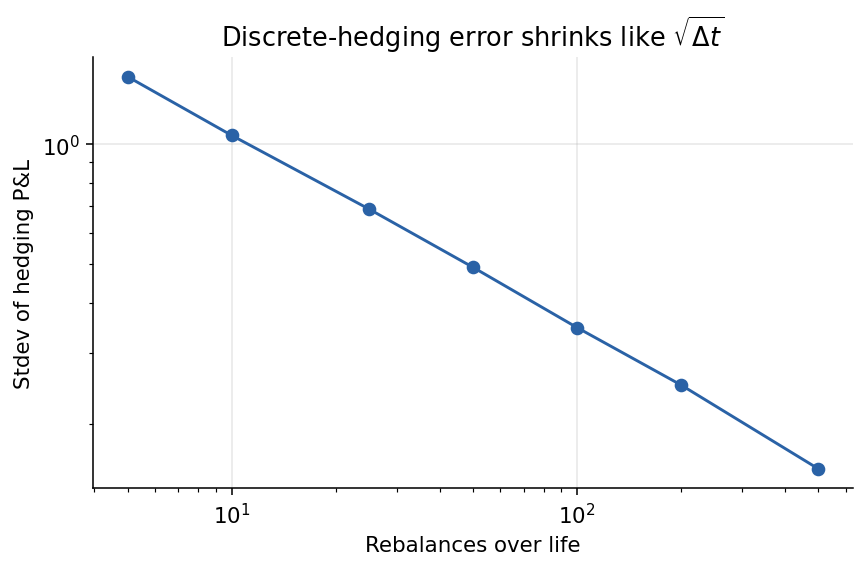
\includegraphics[keepaspectratio]{figures/ch06-hedge-error.png}}
\emph{Discrete-hedging error vs rebalance frequency.}

\pandocbounded{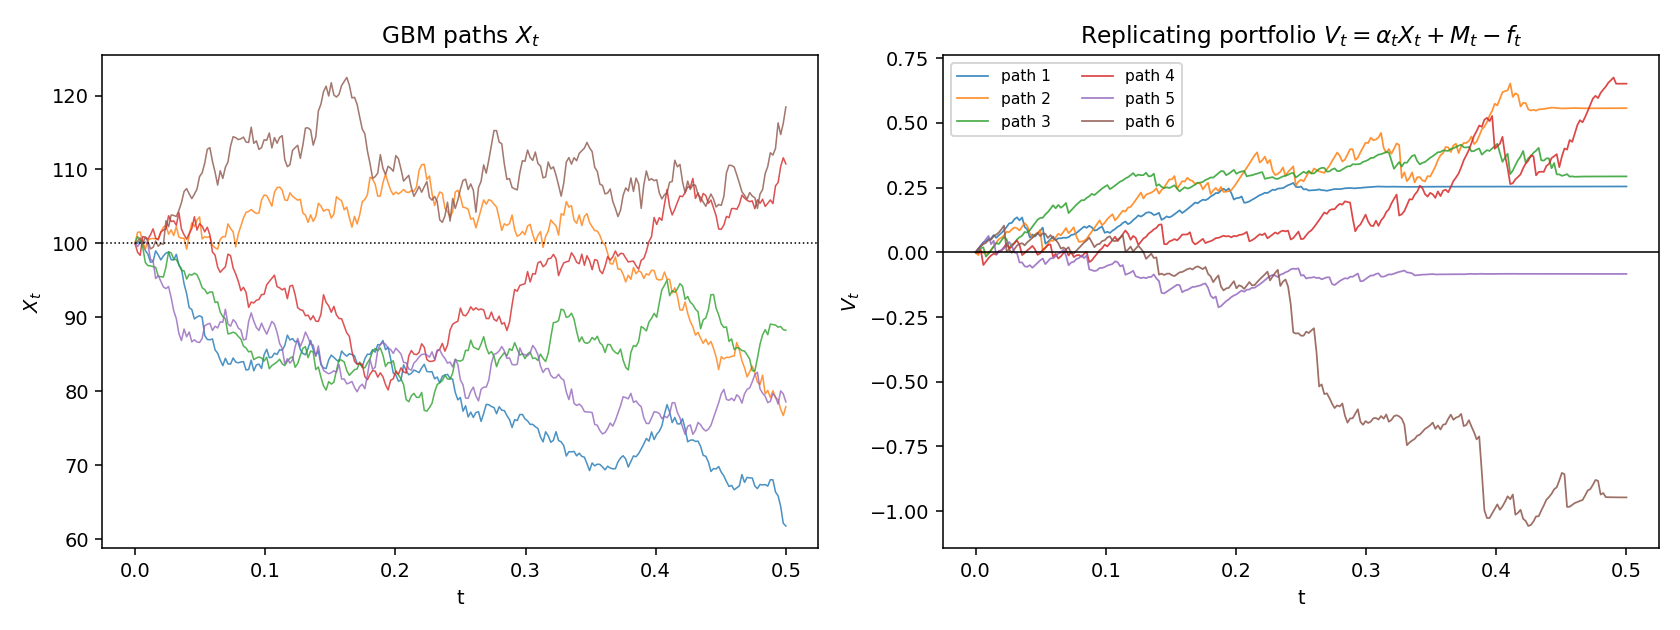
\includegraphics[keepaspectratio]{figures/ch06-replicating-path.png}}
\emph{Ideal continuous hedging would pin \(V_t \equiv 0\); daily
rebalancing leaves visible gamma-driven wiggles.}

\subsection{\texorpdfstring{6.11.7 Shape of \(\alpha_t\) near expiry ---
digital
call}{6.11.7 Shape of \textbackslash alpha\_t near expiry --- digital call}}\label{shape-of-alpha_t-near-expiry-digital-call}

Near \(t = T\), the digital-call delta \(\alpha = \partial_x f\) spikes
around the strike \(K\). A useful way to watch this evolve is to plot
the delta as a function of spot for three representative time slices:

\begin{figure}[H]
\centering
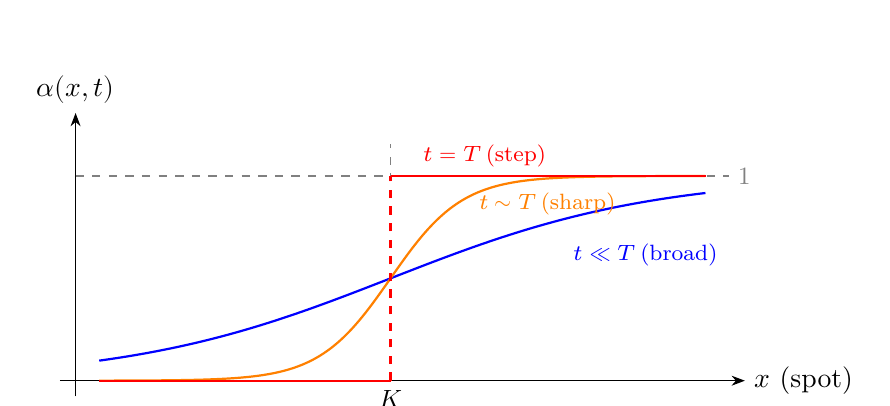
\begin{tikzpicture}[>=Stealth,scale=1.0]
  \draw[->] (-0.2,0) -- (8.5,0) node[right] {$x$ (spot)};
  \draw[->] (0,-0.2) -- (0,3.4) node[above] {$\alpha(x,t)$};
  \draw[dashed,gray] (0,2.6) -- (8.3,2.6) node[right] {\small $1$};
  \draw[dashed,gray] (4,0) -- (4,3.0); \node[below] at (4,0) {\small $K$};
  % t << T : broad logistic
  \draw[thick,blue] plot[domain=0.3:8,smooth,samples=80] (\x,{2.6/(1+exp(-0.6*(\x-4)))});
  % t ~ T : tight sigmoid
  \draw[thick,orange] plot[domain=0.3:8,smooth,samples=120] (\x,{2.6/(1+exp(-2.2*(\x-4)))});
  % t = T : step
  \draw[thick,red] (0.3,0) -- (4,0);
  \draw[thick,red,dashed] (4,0) -- (4,2.6);
  \draw[thick,red] (4,2.6) -- (8,2.6);
  % labels
  \node[blue,anchor=west,font=\footnotesize] at (6.2,1.6) {$t \ll T$ (broad)};
  \node[orange,anchor=west,font=\footnotesize] at (5.0,2.25) {$t \sim T$ (sharp)};
  \node[red,anchor=west,font=\footnotesize] at (4.3,2.85) {$t = T$ (step)};
\end{tikzpicture}

\textit{As $t \to T^-$ the digital-call delta sharpens from a broad logistic into a step at $K$; gamma is the spatial derivative, so it blows up into a Dirac spike at expiry.}
\end{figure}

\begin{itemize}
\tightlist
\item
  \textbf{\(t \ll T\) (far from expiry):} the delta is a broad,
  logistic-looking curve rising gently from near \(0\) on the far left
  through roughly \(\tfrac12\) at \(x = K\) to near \(1\) on the far
  right. Gamma is modest and the hedge is easy to track.
\item
  \textbf{\(t \sim T\) (close to expiry):} the logistic tightens into a
  sharp S-curve concentrated near \(K\). Gamma grows large in a narrow
  band; outside the band the delta is essentially \(0\) or \(1\).
\item
  \textbf{\(t = T\) (at expiry):} the delta jumps from \(0\) to \(1\) at
  \(K\) --- a step function --- and its derivative (gamma) is a Dirac
  \(\delta\)-spike.
\end{itemize}

As \(t \to T^-\) the delta becomes a Dirac at \(K\) --- hedging digitals
near expiry is impossible without discontinuous trades (``delta
blow-up''). Standard remedy: replace the digital by a tight call spread
(long \(K - \epsilon/2\), short \(K + \epsilon/2\), scaled by
\(1/\epsilon\)). The spread's delta is bounded by \(1/\epsilon\);
tighter \(\epsilon\) means closer to a digital but harder to hedge.

\pandocbounded{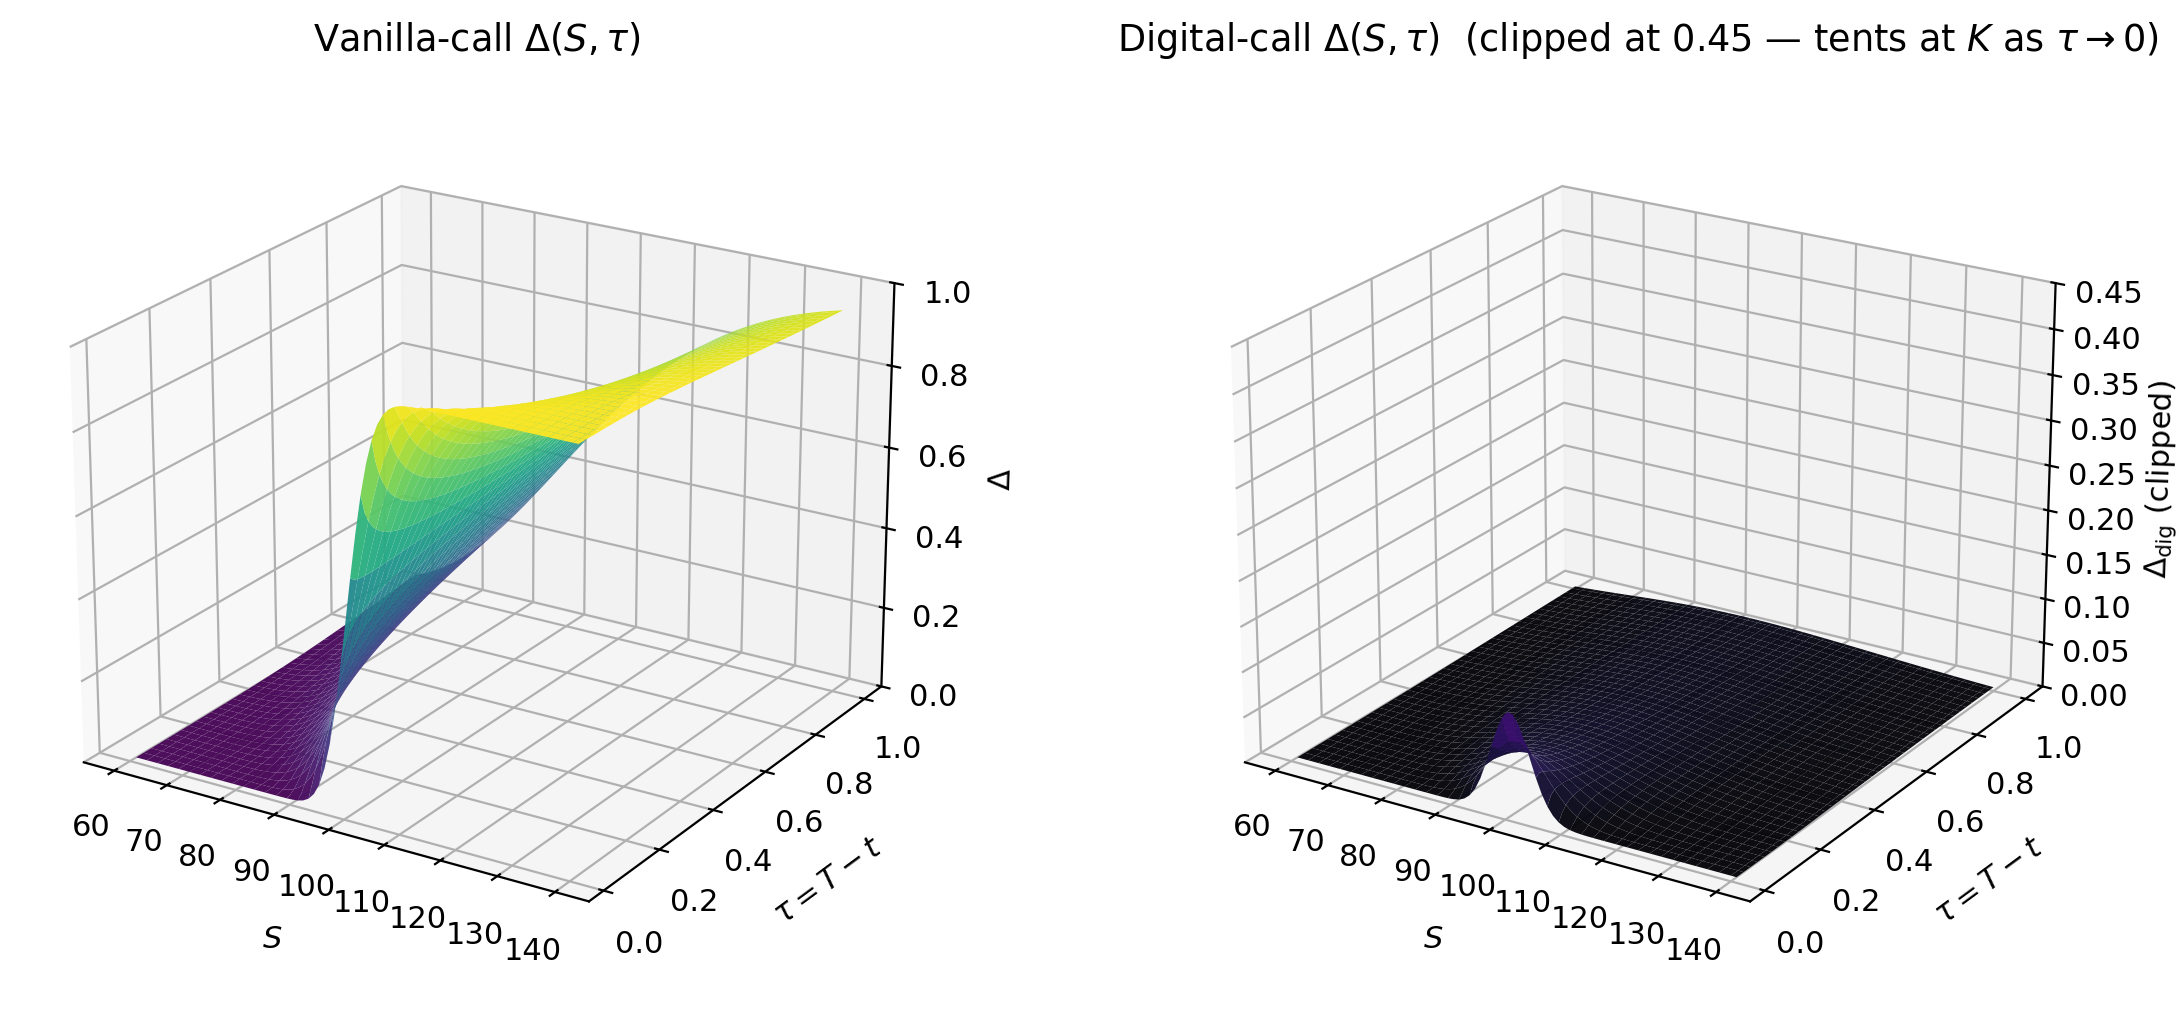
\includegraphics[keepaspectratio]{figures/ch06-delta-surface.png}}
\emph{Left: smooth vanilla delta. Right: digital delta tents at \(K\) as
\(\tau\to 0\) --- the hedger must trade arbitrarily large size around
the strike.}

\begin{center}\rule{0.5\linewidth}{0.5pt}\end{center}

\section{6.12 Move-based hedging}\label{move-based-hedging}

Time-based hedging rebalances on the clock; \textbf{move-based hedging}
rebalances only when the held delta drifts outside a band around the
last-hedged value. The trader cares about \emph{delta error}, not
elapsed time.

\begin{itemize}
\tightlist
\item
  Set a band \([\alpha^\star - \epsilon,\ \alpha^\star + \epsilon]\).
\item
  Let \(\alpha_t\) drift inside the band.
\item
  When \(\alpha_t\) exits, re-centre: new \(\alpha^\star = \alpha_t\),
  restart.
\end{itemize}

\begin{figure}[H]
\centering
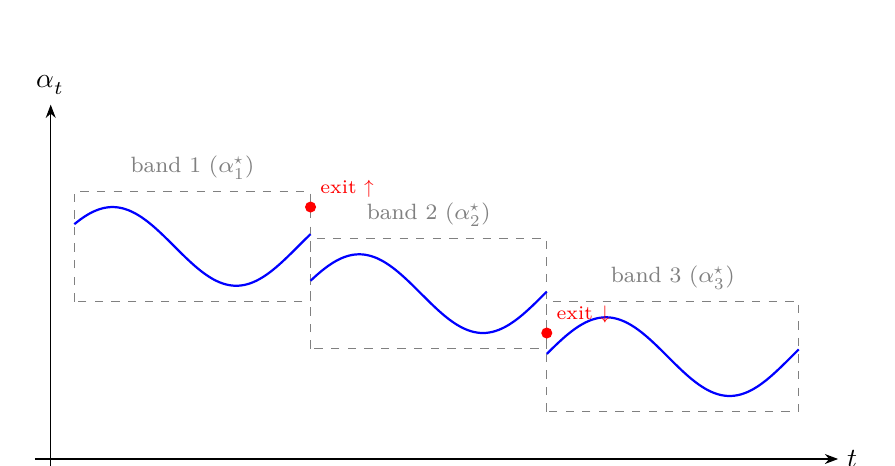
\begin{tikzpicture}[>=Stealth,scale=1.0]
  \draw[->] (-0.2,0) -- (10,0) node[right] {$t$};
  \draw[->] (0,-0.2) -- (0,4.5) node[above] {$\alpha_t$};
  % band 1
  \draw[dashed,gray] (0.3,2.0) rectangle (3.3,3.4);
  \node[gray,font=\footnotesize] at (1.8,3.7) {band 1 ($\alpha^\star_1$)};
  % band 2 (lower, re-centred after upward exit)
  \draw[dashed,gray] (3.3,1.4) rectangle (6.3,2.8);
  \node[gray,font=\footnotesize] at (4.8,3.1) {band 2 ($\alpha^\star_2$)};
  % band 3 (lower again)
  \draw[dashed,gray] (6.3,0.6) rectangle (9.5,2.0);
  \node[gray,font=\footnotesize] at (7.9,2.3) {band 3 ($\alpha^\star_3$)};
  % delta trajectory
  \draw[thick,blue] plot[domain=0.3:3.3,smooth,samples=40] (\x,{2.7+0.5*sin(2*\x r)});
  \draw[thick,blue] plot[domain=3.3:6.3,smooth,samples=40] (\x,{2.1+0.5*sin(2*\x r+1)});
  \draw[thick,blue] plot[domain=6.3:9.5,smooth,samples=40] (\x,{1.3+0.5*sin(2*\x r+2)});
  % exit markers
  \fill[red] (3.3,3.2) circle (2pt) node[above right,font=\scriptsize,red] {exit $\uparrow$};
  \fill[red] (6.3,1.6) circle (2pt) node[above right,font=\scriptsize,red] {exit $\downarrow$};
\end{tikzpicture}

\textit{The delta drifts inside a band of width $2\epsilon$ around the last-hedged value $\alpha^\star$. On exit, a single trade snaps the position to the current $\alpha_t$, and a fresh band re-centres.}
\end{figure}

Move-based trades fewer times than time-based for the same tracking
error on smooth paths, but pays up on rapid gamma swings. The
fundamental dial: expected number of trades scales as \(1/\epsilon^2\)
(Brownian local-time result), tracking error scales linearly in
\(\epsilon\) --- quadratically fewer trades for a linear increase in
noise.

A short ATM 3-month call under GBM, 10 bps/share transaction cost,
varying band \(\epsilon\):

{\def\LTcaptype{none} % do not increment counter
\begin{longtable}[]{@{}lll@{}}
\toprule\noalign{}
Band \(\epsilon\) & Mean P\&L & P\&L std \\
\midrule\noalign{}
\endhead
\bottomrule\noalign{}
\endlastfoot
0.00625 & -0.39 & 0.705 \\
0.0125 & -0.35 & 0.710 \\
0.025 & -0.34 & 0.750 \\
0.05 & -0.34 & 0.850 \\
0.10 & -0.32 & 1.290 \\
0.20 & -0.33 & 2.190 \\
\end{longtable}
}

Wider bands raise mean P\&L (less commission bleed) but inflate std-dev
(delta wanders further). The frontier ``commission + variance''
\(\sim a/\epsilon^2 + b\epsilon^2\) has a clean minimum.

Operationally, layer move-based triggers on a clock baseline and
hard-code rebalances around known events (open, close, earnings,
central-bank meetings) --- these are when path continuity breaks.
Production systems typically use \textbf{delta-dollars}
(\(\Delta \cdot S\)) bands rather than pure delta bands, so limits are
comparable across underlyings of different price levels and feed cleanly
into the desk's risk-limit system. Beyond delta-dollars bands, more
sophisticated desks layer \textbf{gamma-adjusted} bands --- the idea
being that a position with high gamma needs to be rebalanced more often
because its delta moves more per unit of stock move.

In a world with zero transaction costs, continuous rebalancing is
trivially optimal. In a world with finite transaction costs, neither
time-based nor move-based is universally optimal. The modern derivatives
desk uses a hybrid approach, running time-based rebalancing as a
baseline safety net and move-based overlays where they add value. The
chapter's discussion of continuous dynamic hedging is the theoretical
idealisation these practical schemes are trying to approximate.

\begin{center}\rule{0.5\linewidth}{0.5pt}\end{center}

\subsection{Case study (a): Black Monday 1987 --- portfolio insurance
and the dynamic hedge
cascade}\label{case-study-a-black-monday-1987-portfolio-insurance-and-the-dynamic-hedge-cascade}

\emph{Synthetic puts replicated by selling futures into a falling
market.} \emph{The continuous-hedge ideal collided with discrete fills
and a 22\% gap.} \emph{The cohort-level short gamma was the systemic
short option no one had marked.}

\textbf{Context.} Through 1986--87, roughly \$60--90 billion of US
institutional equity was running ``portfolio insurance'' --- a strategy
popularised by Leland-O'Brien-Rubinstein Associates (LOR) and Wells
Fargo Wilshire Investment Management. Mechanically the product was a
synthetic protective put: instead of buying listed SPX puts at their
(rich) implied vol, the manager dynamically replicated the put payoff by
holding equities and dynamically shorting S\&P 500 futures in proportion
to the put's delta. As the index fell, the put's delta moved toward
\(-1\), and the strategy mechanically sold \emph{more} futures to
maintain the hedge. The selling was supposed to be smooth --- small
adjustments against an assumed-continuous price path --- and benign in
normal conditions.

On Friday 16 October 1987 the S\&P 500 closed down 5.16\%, and Monday's
open was already gapping. Through 19 October, the cash index fell from
282.70 to 224.84 (down 20.5\% close-to-close, with intraday lows
touching −22.6\%). Portfolio-insurance programs trying to hedge against
a 5\% move had to reprice deltas against a 20\% move, and the resulting
sell program in the futures pit was estimated at \$14B notional in S\&P
500 and MMI futures over Monday --- into a market where market makers
were on strike, the NYSE specialists could not open dozens of names, and
futures-cash basis blew out to a 20-handle premium then a 60-handle
discount. The Brady Commission's Report (January 1988) named portfolio
insurance and index arbitrage as the two mechanically-amplifying flows.

\textbf{Through the chapter's math.} Three failure modes of the
Black-Scholes hedge framework lined up. (i) The hedge ratio
\(\alpha_t = \partial_x f(t, X_t)\) from §6.3 is \emph{continuous} in
\(S\), but fills are discrete: when \(S\) gaps from 282 to 225 with no
quotes in between, you cannot trade the intermediate deltas --- you go
straight to the post-gap delta and book the path-dependent gamma loss in
one print. (ii) The local Itô expansion (6.6) reads
\(\mathrm dV_t \approx \alpha_t\,\mathrm dS_t + \tfrac12 \Gamma_t (\mathrm dS_t)^2\)
under the assumption \((\mathrm dS_t)^2 = \sigma^2 S_t^2\,\mathrm dt\);
when the realised \((\Delta S)^2 / S^2\) is on the order of 0.05 instead
of \(\sigma^2 \cdot \Delta t \approx 0.0001\), the discrete-hedging
error of §6.11.6 is two orders of magnitude past its \(\sqrt{\Delta t}\)
scaling estimate. (iii) Each LOR client's program was independently
short gamma to its hedger --- but at the \emph{cohort} level the entire
\$80B of insurance flow was net short gamma against the same index, and
that aggregate gamma exposure had no second-leg hedger because the
synthetic-put issuer was the market itself. The market's effective
short-gamma position showed up as a price impact term that the dynamic
hedge had to chase.

\textbf{Lesson.} The ``synthetic put'' was synthetic until it wasn't.
The chapter's continuous-time replication argument in §6.2--6.3 promises
a perfect hedge under (a) frictionless markets, (b) continuous price
paths, and (c) an outside-counterparty buyer for whatever delta the
hedger needs to trade. October 1987 violated all three at once. The
modern legacy of 1987 is structural: SPX listed put open interest is
materially higher than its 1980s level (insurers buy listed puts now
rather than synthesise them), exchange circuit breakers institutionalise
the gap-discontinuity acknowledgement, and any desk running synthetic
optionality calculates a ``if the market gapped 10\% before I could
rebalance'' stress P\&L as a regulatory risk metric. The
Brady-Commission view --- that any hedging strategy whose required
trades scale with realised moves can become destabilising at scale ---
is now baked into SEC Rule 15c3-5 (market access) and the post-crisis
trade-through controls. Portfolio insurance the product still exists,
but is sized to remain a price-taker, not a price-maker.

\begin{center}\rule{0.5\linewidth}{0.5pt}\end{center}

\subsection{Case study (b): GameStop January 2021 --- gamma squeeze as
forced
delta-hedge}\label{case-study-b-gamestop-january-2021-gamma-squeeze-as-forced-delta-hedge}

\emph{Retail call buying forces market makers into mechanical buying.}
\emph{Positive gamma on the MM short means \(\delta' = \Gamma > 0\) in
\(S\).} \emph{The ``gamma squeeze'' headline is just (6.6) read out
loud.}

\textbf{Context.} Through January 2021, retail call-option buying on
GameStop (GME) intensified through the WallStreetBets community on
Reddit. Daily GME call volume on weekly and front-month expiries reached
six- to ten-times historical norms; on 22 January, GME call open
interest exceeded the entire free-float share count. Market makers ---
predominantly Citadel Securities, Susquehanna, Wolverine, and Group One
on the option side --- fill these option orders by selling calls and
dynamically delta- hedging the resulting short. The implied vol the MM
charged was high (IV on GME 30-day options jumped from
\textasciitilde80\% to over 400\% in that two-week window), but the
dynamic-hedge mechanics were exactly what §6.3 describes: sell call →
short delta → buy stock to be flat.

The GME spot ran from \$19.94 (4 Jan close) to \$325.00 (29 Jan close),
a 16× move in twenty trading days, with intraday peaks at \$483 on 28
January. Each new call buyer added incremental short-gamma exposure to
the MM book, the MM bought more stock to re-flatten delta, that buying
contributed to the very price rise that pushed the next strike's delta
into the hedger's must-buy zone. Retail brokers (notably Robinhood) at
the peak suspended buy-side orders in GME on 28 January citing
clearinghouse margin requirements, snapping the feedback loop.

\textbf{Through the chapter's math.} The market-maker's hedged book is
\(V^{\text{MM}}_t = -C(t, S_t) + \alpha_t S_t + \beta_t M_t\) with
\(\alpha_t = \partial_S C\) --- the call's delta. Itô on \(C\) gives
\(\mathrm dC = \partial_t C\,\mathrm dt + \partial_S C\,\mathrm dS_t + \tfrac12 \partial_{SS} C \cdot \sigma^2 S_t^2\,\mathrm dt\),
so the MM's short-call \(\Gamma\) exposure is
\(-\partial_{SS} C = -\Gamma_t < 0\) (short gamma). The required delta
adjustment per move in \(S\) is
\(\mathrm d\alpha_t = \Gamma_t\,\mathrm dS_t\): \(S\) goes up by
\(\Delta S\), the MM must \emph{buy} \(\Gamma_t \cdot \Delta S\) extra
shares to remain delta-neutral. With aggregate dealer dollar-gamma on
GME estimated at \$200--400M per percentage-point move at the peak, a
1\% spot move forced
\textasciitilde{}\(3M in mechanical buying *from the hedge alone*,
on top of underlying retail order flow. The dollar-gamma metric
(\)\$\Gamma = \Gamma\_t \cdot S\_t\^{}2 \cdot 0.01\$) --- the dealer's
mechanical buy/sell pressure per 1\% move --- is the single number that
diagnoses this dynamic, and is the version of §6.3 that risk managers
now publish on positioning dashboards alongside the SPX itself.

\textbf{Lesson.} The ``gamma squeeze'' is not a market-microstructure
exotic or a coordinated retail attack --- it is the §6.3 hedge ratio
applied at scale to a name with thin float and concentrated short-gamma
dealer positioning. The right diagnostic is dollar-gamma at the
underlying level, aggregated across all listed strikes weighted by open
interest; when dollar-gamma exceeds a meaningful fraction of average
daily volume, the dealer hedge becomes price-impacting and the
underlying becomes gamma-driven rather than fundamental-driven.
Post-GME, every prime broker's risk team publishes dealer-positioning
estimates by name; SEC Staff Report on Equity and Options Market
Structure Conditions in Early 2021 (October 2021) documents the
mechanism in detail and uses exactly this language. The deeper lesson
for the dynamic-hedging chapter: \(\Gamma > 0\) for the long-call holder
is what makes the convexity of options valuable; the same \(\Gamma\) on
the MM's short side, multiplied by enough notional, becomes a
market-moving exogenous demand curve.

\begin{center}\rule{0.5\linewidth}{0.5pt}\end{center}

\subsection{Case study (c): Volmageddon February 5 2018 --- XIV
liquidation via short-vol
gamma}\label{case-study-c-volmageddon-february-5-2018-xiv-liquidation-via-short-vol-gamma}

\emph{Short-vol products are short vol-of-vol --- a hidden second-order
risk.} \emph{Discrete vega rebalancing fails when the vol regime changes
intraday.} \emph{The hedging-error variance scales with
\(\sqrt{\Delta t}\) until it doesn't.}

\textbf{Context.} Credit Suisse's VelocityShares Daily Inverse VIX
Short-Term ETN (ticker XIV, \$1.9B AUM into 5 Feb 2018) and the
structurally related ProShares Short VIX Short-Term Futures ETF (SVXY,
\$0.8B AUM) delivered the inverse of the daily return of the S\&P 500
VIX Short-Term Futures Index --- i.e., a daily reset
short-front-VIX-futures position. Through 2017 the VIX averaged 11.1
(the lowest annual mean since the index began in 1990), and XIV had
returned over 180\% YTD by end-January 2018. The product was popular
with risk-parity and yield-pickup allocators precisely because its
drawdowns had been mild for half a decade.

On Friday 2 February 2018, the SPX closed −2.1\% and the VIX closed at
17.16 (up from 13.47). On Monday 5 February the SPX dropped a further
4.10\%; the VIX intraday spiked from 17 to 50, with the close at 37.32.
The XIV NAV calculation on the issuer's terms triggered an
``acceleration event'' --- a same-day liquidation provision tripped when
the index lost more than 80\% intraday --- and Credit Suisse called the
note for redemption. XIV closed Monday at \$7.35, down from \$115.55
(down 96.3\%), and was wound down weeks later. The operative dynamic was
that the issuers running short-vol replication books were short VIX
futures delta and short vol-of-vol; as VIX rose, they had to \emph{buy}
VIX futures to maintain the short-vega hedge, and the buying happened in
the most illiquid window of the day (the post-3:30 PM ET VIX-future
settlement print), accelerating the spike.

\textbf{Through the chapter's math.} A short-vol position has a P\&L of
the form \(V_t = -F(\sigma_t)\) where \(\sigma_t\) is the relevant vol
process and \(F\) is the structure's payoff in vol.~The first-order risk
is short-vega: \(\partial V/\partial \sigma < 0\). The second-order risk
(volga, \(\partial^2 V/\partial \sigma^2\)) is what blows up in a vol
regime change --- Heston (Chapter 10) parameterises this through the
vol-of-vol parameter \(\xi\), and the volga exposure is large precisely
when \(\xi\) is large. The discrete-hedging error of §6.11.6, repeated
for the vega leg, gives a tracking error of order \(\xi\sqrt{\Delta t}\)
per rebalance interval under stable-regime conditions; the issue is that
when \(\xi\) itself jumps (vol-of-vol on VIX rose from
\textasciitilde80\% on 2 Feb to over 250\% on 5 Feb implied), the hedge
error scales with the new \(\xi^{\text{new}}\) but the hedge ratio is
set against \(\xi^{\text{old}}\) --- the once-a-day vega rebalance
bookmarks a vega number that is wrong within minutes of the next print.
The XIV NAV, mechanically defined as the daily-reset inverse-return, was
effectively a margin-style stop that guaranteed forced covering at the
worst possible vol-of-vol level.

\textbf{Lesson.} A short-vega book that prices and hedges as if vega is
a constant is, in Heston language, ignoring volga. The §6.11 discrete
hedging analysis told us that BS hedge errors scale with
\(\sqrt{\Delta t}\) under the \emph{model's own assumption} that
\(\sigma\) is constant; the moment \(\sigma\) becomes stochastic with
non-trivial vol-of-vol, that \(\sqrt{\Delta t}\) scaling is replaced by
something proportional to the realised \(\xi\), which can be ten times
the calibrated \(\xi\) in a regime change. The lesson is operational and
structural: any short-convexity book must (i) set a hard limit on
vega-by-vol-bucket so a single regime change cannot eat the desk, (ii)
hedge volga explicitly via long out-of-the-money options on the vol
underlying, not just vega via ATM, and (iii) treat the once-a-day
rebalance as inadequate for short- vol books in stressed vol regimes ---
XIV-style products that mechanically rebalance once per day at the close
are \emph{guaranteed} to underperform a continuously-hedged equivalent
in a vol blow-out, by exactly the square-root-of-time argument the
chapter develops, applied to the wrong \(\xi\). The post-2018 short-vol
ETP space halved in AUM and restructured into products with intraday
rebalancing or capped daily loss; the underlying mathematics was a
textbook §6.11 hedging-error cascade applied to the wrong-order Greek.

\begin{center}\rule{0.5\linewidth}{0.5pt}\end{center}

\section{6.13 Key Takeaways}\label{key-takeaways-5}

\begin{enumerate}
\def\labelenumi{\arabic{enumi}.}
\item
  \textbf{Self-financing constraint.} A portfolio
  \((\alpha_t, \beta_t)\) in the underlying and bank account is
  self-financing iff
  \(\mathrm dV_t = \alpha_t\,\mathrm d g_t + \beta_t\,\mathrm d M_t\)
  with \emph{no} fresh injection of cash. Naïve differentiation would
  add a \(g_t\,\mathrm d\alpha_t + M_t\,\mathrm d\beta_t\) term that has
  no economic meaning; the missing term is what arbitrage-free pricing
  forbids.
\item
  \textbf{Delta is \(\partial_x f\).} Locally cancelling the Brownian
  increment in the hedged portfolio forces
  \(\alpha_t = \partial_x f(t, X_t)\) --- the hedge ratio is the slope
  of the pricing function with respect to the underlying, evaluated at
  the current state. No optimisation is required; it falls out of ``set
  the \(\mathrm dW\) coefficient to zero.''
\item
  \textbf{Market price of risk = Girsanov shift.} Equating Sharpe ratios
  across two tradables driven by the same Brownian gives
  \(\lambda = (\mu^f - r)/\sigma^f = (\mu^g - r)/\sigma^g\), the
  \textbf{market price of risk} --- universal across hedgeable assets by
  no-arbitrage. Read through Chapter 5, \(\lambda\) is the integrand of
  the Radon-Nikodym density that takes \(\mathbb{P}\) to \(\mathbb{Q}\).
\item
  \textbf{Generalised BS PDE (6.24).} For an underlying
  \(\mathrm dX_t = \mu^x\,\mathrm dt + \sigma^x\,\mathrm dW_t\) with
  state-dependent coefficients, the option price \(f(t, x)\) satisfies
  \(\partial_t f + (\mu^x - \sigma^x \lambda)\,\partial_x f + \tfrac12 (\sigma^x)^2\,\partial_{xx} f = r\,f\)
  with terminal data \(f(T, x) = \varphi(x)\). The physical drift
  \(\mu^x\) enters only through the combination
  \(\mu^x - \sigma^x \lambda\).
\item
  \textbf{GBM specialisation (6.27)} and \textbf{call formula (6.28).}
  For GBM
  \(\mathrm dX_t = \mu X_t\,\mathrm dt + \sigma X_t\,\mathrm dW_t\), the
  PDE collapses to
  \(\partial_t f + r x \partial_x f + \tfrac12 \sigma^2 x^2 \partial_{xx} f = r f\).
  The European call solution is
  \(f(t, x) = x\,\Phi(d_+) - K e^{-r(T - t)}\,\Phi(d_-)\) with
  \(d_\pm = [\ln(x/K) + (r \pm \tfrac12 \sigma^2)(T - t)]/(\sigma\sqrt{T-t})\).
  The physical drift \(\mu\) is absent --- option prices do not depend
  on the underlying's expected return.
\item
  \textbf{Closed-form vanilla Greeks.}
  \(\Delta^C = \Phi(d_+) \in (0, 1)\),
  \(\Gamma^C = \phi(d_+)/(x\sigma\sqrt{T-t})\), vega
  \(\mathcal{V}^C = x\,\phi(d_+)\,\sqrt{T-t}\). Put-call parity gives
  \(\Delta^P = \Delta^C - 1\), \(\Gamma^P = \Gamma^C\),
  \(\mathcal{V}^P = \mathcal{V}^C\).
\item
  \textbf{PDE ⇔ Q-expectation via Feynman-Kac.} The same PDE (6.27) is
  the Feynman-Kac PDE for the discounted \(\mathbb{Q}\)-expectation
  \(f(t, x) = \mathbb{E}^{\mathbb{Q}}_{t, x}[e^{-r(T - t)}\,\varphi(X_T)]\),
  where under \(\mathbb{Q}\) the drift of \(X\) is shifted from \(\mu\)
  to \(r\). Replication, PDE, and risk-neutral expectation are three
  equivalent statements of the same no-arbitrage fact.
\item
  \textbf{Risk-neutral drift = Girsanov-shifted physical drift.}
  \(\mathrm dX_t = \mu X_t\,\mathrm dt + \sigma X_t\,\mathrm dW_t = r X_t\,\mathrm dt + \sigma X_t\,\mathrm d\widetilde W_t\)
  with \(\widetilde W_t = W_t + \lambda t\) (Eq. 6.51-6.52). The
  bank-account-deflated price \(e^{-rt}\,X_t\) is a
  \(\mathbb{Q}\)-martingale, as is \(e^{-rt}\,f_t\).
\item
  \textbf{Discrete-hedging recursion (6.56) and \(\sqrt{\Delta t}\)
  tracking error.} With holdings \(\alpha_t = \partial_x f\) rebalanced
  on a grid \(\{t_0, \ldots, t_N\}\), the bank balance evolves as
  \(M_{t_n} = M_{t_{n-1}}\,e^{r\,\Delta t} - (\alpha_{t_n} - \alpha_{t_{n-1}})\,X_{t_n}\).
  Terminal P\&L (Eq. 6.58) has mean zero under correct model
  specification; its standard deviation scales as \(\sqrt{\Delta t}\)
  --- doubling rebalance frequency cuts hedging error by \(\sqrt 2\),
  not 2.
\item
  \textbf{Gamma · (realised − implied) P\&L identity.} The leading-order
  single-step P\&L from a mis-specified implied volatility is
  \(\tfrac12\,\Gamma\,S^2\,(\sigma_{\text{realised}}^2 - \sigma_{\text{implied}}^2)\,\Delta t\).
  A long-gamma position earns money when realised variance exceeds the
  implied number priced into the option; a short-gamma position bleeds
  the variance risk premium. Every variance-swap and gamma-trading
  strategy in the guide reduces to this identity.
\item
  \textbf{Digital Greeks blow up like \(1/\sqrt{T-t}\).} At-the-money on
  expiration day, the digital call's delta
  \(e^{-r(T-t)}\phi(d_-)/(x\sigma\sqrt{T-t})\) diverges as
  \(T - t \to 0\) because \(\phi(d_-) \to \phi(0) = 1/\sqrt{2\pi}\)
  stays bounded while \(\sqrt{T-t} \to 0\). This is the
  \textbf{pin-risk} phenomenon and is the reason desks tame digital
  exposures with call-spread replication.
\item
  \textbf{Move-based vs time-based hedging trade-off.} Time-based
  rebalancing has \(\sqrt{\Delta t}\) error and predictable
  transaction-cost frequency; move-based (``rebalance when
  \$\textbar{}\Delta(t, S) - \alpha\_t\textbar{} \textgreater{} \$
  band'') concentrates rebalances around the at-the-money region where
  gamma is large. With finite transaction costs neither is universally
  optimal; production desks hybridise --- time-based safety net plus
  move-based overlay, both quoted in \textbf{delta-dollars} so positions
  compare across underlyings.
\item
  \textbf{The hedger's price is drift-free.} Two stocks with the same
  \(\sigma\) but different physical drifts \(\mu\) have identical call
  prices. The hedger replicates payoffs state-by-state; the cost depends
  on how hard the replication machine has to work, which scales with
  vol, not drift.
\item
  \textbf{Implied volatility is forecast volatility (under
  \(\mathbb{Q}\)).} A 20\% ATM implied vol is the market's unbiased
  estimate of the root-mean-square log-return over the option's life
  \emph{under the risk-neutral measure}. Under \(\mathbb{P}\) it can be
  a touch lower because \(\mathbb{Q}\) overweights downside; for liquid
  equity options the gap is small.
\end{enumerate}

\begin{center}\rule{0.5\linewidth}{0.5pt}\end{center}

\section{6.14 Reference Formulas
Appendix}\label{reference-formulas-appendix}

\subsection{6.14.1 Setup and SDE
coefficients}\label{setup-and-sde-coefficients}

{\def\LTcaptype{none} % do not increment counter
\begin{longtable}[]{@{}
  >{\raggedright\arraybackslash}p{(\linewidth - 2\tabcolsep) * \real{0.5000}}
  >{\raggedright\arraybackslash}p{(\linewidth - 2\tabcolsep) * \real{0.5000}}@{}}
\toprule\noalign{}
\begin{minipage}[b]{\linewidth}\raggedright
Quantity
\end{minipage} & \begin{minipage}[b]{\linewidth}\raggedright
Symbol / formula
\end{minipage} \\
\midrule\noalign{}
\endhead
\bottomrule\noalign{}
\endlastfoot
Underlying SDE (general) &
\(\mathrm dX_t = \mu^x(t, X_t)\,\mathrm dt + \sigma^x(t, X_t)\,\mathrm dW_t\) \\
Underlying SDE (GBM specialisation) &
\(\mathrm dS_t/S_t = \mu\,\mathrm dt + \sigma\,\mathrm dW_t\) \\
Bank account & \(\mathrm dM_t/M_t = r_t\,\mathrm dt\), \(M_0 = 1\) \\
Self-financing portfolio & \(V_t = \alpha_t g_t + \beta_t M_t\),
\(\mathrm dV_t = \alpha_t\,\mathrm dg_t + \beta_t\,\mathrm dM_t\) \\
Delta-hedge ratio & \(\alpha_t = \partial_x f(t, X_t)\) \\
Market price of risk &
\(\lambda(t, x) = (\mu^f - r)/\sigma^f = (\mu^g - r)/\sigma^g = (\mu^x - r x \cdot \mathbb{1}_{\text{tradable } X})/\sigma^x\) \\
\(\mathbb{Q}\)-dynamics (Girsanov-shifted) &
\(\mathrm dX_t = (\mu^x - \sigma^x \lambda)\,\mathrm dt + \sigma^x\,\mathrm d\widetilde W_t\),
\(\widetilde W_t = W_t + \int_0^t \lambda\,\mathrm du\) \\
\end{longtable}
}

\subsection{6.14.2 BS PDE --- three equivalent
forms}\label{bs-pde-three-equivalent-forms}

{\def\LTcaptype{none} % do not increment counter
\begin{longtable}[]{@{}
  >{\raggedright\arraybackslash}p{(\linewidth - 4\tabcolsep) * \real{0.3333}}
  >{\raggedright\arraybackslash}p{(\linewidth - 4\tabcolsep) * \real{0.3333}}
  >{\raggedright\arraybackslash}p{(\linewidth - 4\tabcolsep) * \real{0.3333}}@{}}
\toprule\noalign{}
\begin{minipage}[b]{\linewidth}\raggedright
Form
\end{minipage} & \begin{minipage}[b]{\linewidth}\raggedright
Equation
\end{minipage} & \begin{minipage}[b]{\linewidth}\raggedright
Eq.
\end{minipage} \\
\midrule\noalign{}
\endhead
\bottomrule\noalign{}
\endlastfoot
Generalised BS PDE &
\(\partial_t f + (\mu^x - \sigma^x \lambda)\,\partial_x f + \tfrac12 (\sigma^x)^2\,\partial_{xx} f = r f\),
\(f(T, x) = \varphi(x)\) & \((6.24)\) \\
GBM specialisation &
\(\partial_t f + r x\,\partial_x f + \tfrac12 \sigma^2 x^2\,\partial_{xx} f = r f\),
\(f(T, x) = \varphi(x)\) & \((6.27)\) \\
\(\mathbb{Q}\)-expectation (Feynman-Kac) &
\(f(t, x) = \mathbb{E}^{\mathbb{Q}}_{t, x}[e^{-r(T-t)}\,\varphi(X_T)]\),
\(\mathrm dX_s = r X_s\,\mathrm ds + \sigma X_s\,\mathrm d\widetilde W_s\)
& \((6.50)\) \\
\end{longtable}
}

\subsection{\texorpdfstring{6.14.3 Closed-form vanilla Greeks
(\(d_\pm = [\ln(x/K) + (r \pm \tfrac12 \sigma^2)(T-t)]/(\sigma\sqrt{T-t})\))}{6.14.3 Closed-form vanilla Greeks (d\_\textbackslash pm = {[}\textbackslash ln(x/K) + (r \textbackslash pm \textbackslash tfrac12 \textbackslash sigma\^{}2)(T-t){]}/(\textbackslash sigma\textbackslash sqrt\{T-t\}))}}\label{closed-form-vanilla-greeks-d_pm-lnxk-r-pm-tfrac12-sigma2t-tsigmasqrtt-t}

{\def\LTcaptype{none} % do not increment counter
\begin{longtable}[]{@{}
  >{\raggedright\arraybackslash}p{(\linewidth - 8\tabcolsep) * \real{0.2000}}
  >{\raggedright\arraybackslash}p{(\linewidth - 8\tabcolsep) * \real{0.2000}}
  >{\raggedright\arraybackslash}p{(\linewidth - 8\tabcolsep) * \real{0.2000}}
  >{\raggedright\arraybackslash}p{(\linewidth - 8\tabcolsep) * \real{0.2000}}
  >{\raggedright\arraybackslash}p{(\linewidth - 8\tabcolsep) * \real{0.2000}}@{}}
\toprule\noalign{}
\begin{minipage}[b]{\linewidth}\raggedright
Contract
\end{minipage} & \begin{minipage}[b]{\linewidth}\raggedright
Price
\end{minipage} & \begin{minipage}[b]{\linewidth}\raggedright
Delta
\end{minipage} & \begin{minipage}[b]{\linewidth}\raggedright
Gamma
\end{minipage} & \begin{minipage}[b]{\linewidth}\raggedright
Vega
\end{minipage} \\
\midrule\noalign{}
\endhead
\bottomrule\noalign{}
\endlastfoot
Call \(\varphi(x) = (x - K)^+\) &
\(x\,\Phi(d_+) - K e^{-r(T-t)}\,\Phi(d_-)\) & \(\Phi(d_+)\) &
\(\dfrac{\phi(d_+)}{x\sigma\sqrt{T-t}}\) & \(x\,\phi(d_+)\sqrt{T-t}\) \\
Put \(\varphi(x) = (K - x)^+\) &
\(K e^{-r(T-t)}\,\Phi(-d_-) - x\,\Phi(-d_+)\) & \(\Phi(d_+) - 1\) &
\(\dfrac{\phi(d_+)}{x\sigma\sqrt{T-t}}\) & \(x\,\phi(d_+)\sqrt{T-t}\) \\
Digital call \(\varphi = \mathbf{1}_{\{x > K\}}\) &
\(e^{-r(T-t)}\,\Phi(d_-)\) &
\(e^{-r(T-t)}\dfrac{\phi(d_-)}{x\sigma\sqrt{T-t}}\) &
\(-e^{-r(T-t)}\dfrac{d_+\,\phi(d_-)}{x^2\sigma^2(T-t)}\) &
\(-e^{-r(T-t)}\dfrac{d_+\,\phi(d_-)}{\sigma}\) \\
\end{longtable}
}

Strike-shifting identity: \(x\,\phi(d_+) = K e^{-r(T-t)}\,\phi(d_-)\).
Put-call parity: \(C_t - P_t = x - K e^{-r(T-t)}\), hence
\(\Delta^P = \Delta^C - 1\), \(\Gamma^P = \Gamma^C\),
\(\mathcal V^P = \mathcal V^C\). Pin-risk fingerprint: digital delta
\(\sim 1/\sqrt{T-t}\) as \(t \to T\) at \(x = K\).

\subsection{\texorpdfstring{6.14.4 Discrete hedging --- recursion and
\(\sqrt{\Delta t}\)
scaling}{6.14.4 Discrete hedging --- recursion and \textbackslash sqrt\{\textbackslash Delta t\} scaling}}\label{discrete-hedging-recursion-and-sqrtdelta-t-scaling}

{\def\LTcaptype{none} % do not increment counter
\begin{longtable}[]{@{}
  >{\raggedright\arraybackslash}p{(\linewidth - 4\tabcolsep) * \real{0.3333}}
  >{\raggedright\arraybackslash}p{(\linewidth - 4\tabcolsep) * \real{0.3333}}
  >{\raggedright\arraybackslash}p{(\linewidth - 4\tabcolsep) * \real{0.3333}}@{}}
\toprule\noalign{}
\begin{minipage}[b]{\linewidth}\raggedright
Quantity
\end{minipage} & \begin{minipage}[b]{\linewidth}\raggedright
Formula
\end{minipage} & \begin{minipage}[b]{\linewidth}\raggedright
Eq.
\end{minipage} \\
\midrule\noalign{}
\endhead
\bottomrule\noalign{}
\endlastfoot
Bank-balance recursion &
\(M_{t_n} = M_{t_{n-1}}\,e^{r\,\Delta t} - (\alpha_{t_n} - \alpha_{t_{n-1}})\,X_{t_n}\)
& \((6.56)\) \\
With transaction cost \(\kappa\) &
\(M_k = M_{k-1}\,e^{r\,\Delta t_k} - (\alpha_k - \alpha_{k-1})\,S_k - \kappa(\alpha_k - \alpha_{k-1})\)
& \((6.57)\) \\
Terminal P\&L (no costs) &
\(\mathrm{PnL} = (M_{t_{N-1}}\,e^{r\,\Delta t} + \alpha_{t_{N-1}}\,X_{t_N}) - \varphi(X_{t_N})\)
& \((6.58)\) \\
Per-step P\&L residual &
\(\tfrac12\,\Gamma\,S^2\,\sigma^2\,(Z^2 - 1)\,\Delta t\),
\(Z \sim \mathcal N(0, 1)\) & \\
Tracking-error std-dev scaling &
\(\mathrm{std}(\mathrm{PnL}) \sim \Gamma\,S^2\,\sigma^2\,\sqrt{T\,\Delta t}\)
& \\
Gamma · realised-vs-implied identity &
\(\Delta\Pi \approx \tfrac12\,\Gamma\,S^2\,(\sigma_{\mathrm{realised}}^2 - \sigma_{\mathrm{implied}}^2)\,\Delta t\)
& \\
\end{longtable}
}

\newpage

\chapter{Chapter 7 --- Dynamic Hedging II: Greeks, Delta-Gamma, Vega,
and
Dividends}\label{chapter-7-dynamic-hedging-ii-greeks-delta-gamma-vega-and-dividends}

Ch. 6 built the single-instrument delta hedge, the generalised BS PDE,
and the vanilla Greeks. Here we enlarge the hedging basis --- first to
neutralise curvature (delta-gamma), then volatility (vega), then
dividends --- and account for transaction costs. The Itô machinery is
unchanged; what grows is the hedge basis.

\section{7.0 Chapter orientation}\label{chapter-orientation}

A delta hedge is \emph{first-order} risk-free: the \(\mathrm{d}W_t\)
coefficient is zero, but residual exposures live in the higher-order
terms. Gamma is the coefficient of \((\Delta S)^2\), vega of
\(\Delta\sigma\), theta of \(\Delta t\). Cross-derivatives (vanna,
volga, charm, speed, colour) parameterise the rest.

Most higher Greeks are not hedgeable with the stock alone --- stock has
zero gamma, zero vega. To kill curvature or vol-level risk we add
another traded option. The linear algebra is easy; the bookkeeping is
where the subtleties live.

Notation as in Ch. 6: \(S_t\) stock, \(g(t, S)\) a claim,
\(\Delta = \partial_S g\), \(\Gamma = \partial_{SS} g\),
\(\mathcal{V} = \partial_\sigma g\). Expectations under \(\mathbb{Q}\).

\begin{center}\rule{0.5\linewidth}{0.5pt}\end{center}

\section{7.1 Greeks recap --- a bridge from Chapter
6}\label{greeks-recap-a-bridge-from-chapter-6}

Catalogue the partials. Let \(g(t, S; \sigma, r)\) price a European
claim. \emph{First-order:}

\[
\Delta_t \;\equiv\; \partial_S g, \qquad
\Theta_t \;\equiv\; \partial_t g, \qquad
\mathcal{V}_t \;\equiv\; \partial_\sigma g, \qquad
\rho_t \;\equiv\; \partial_r g. \tag{7.1}
\]

\emph{Second-order:}

\[
\Gamma_t \;\equiv\; \partial_{SS} g, \qquad
\text{vanna}_t \;\equiv\; \partial_{S\sigma} g, \qquad
\text{volga}_t \;\equiv\; \partial_{\sigma\sigma} g, \qquad
\text{charm}_t \;\equiv\; \partial_{St} g. \tag{7.2}
\]

Third-order Greeks (speed, colour, zomma) characterise tighter
residuals. European call closed forms:

\[
\Delta_{\mathrm{call}} \;=\; \Phi(d_+), \qquad
\Gamma \;=\; \frac{\Phi'(d_+)}{S\,\sigma\sqrt{T-t}}, \qquad
\mathcal{V} \;=\; S\,\sqrt{T-t}\,\Phi'(d_+), \tag{7.3}
\]

and for a European put,
\(\Delta_{\mathrm{put}} = \Phi(d_+) - 1 = -\Phi(-d_+)\), with the same
\(\Gamma\) and \(\mathcal{V}\) as the call (we will prove the gamma
identity via put-call parity in §7.6). Here \(\Phi\) and \(\Phi'\) are
the standard normal CDF and density, and \(d_\pm = [\ln(S/K) + (r \pm
\tfrac{1}{2}\sigma^2)(T-t)] / (\sigma\sqrt{T-t})\) is the Black-Scholes
moneyness index.

\pandocbounded{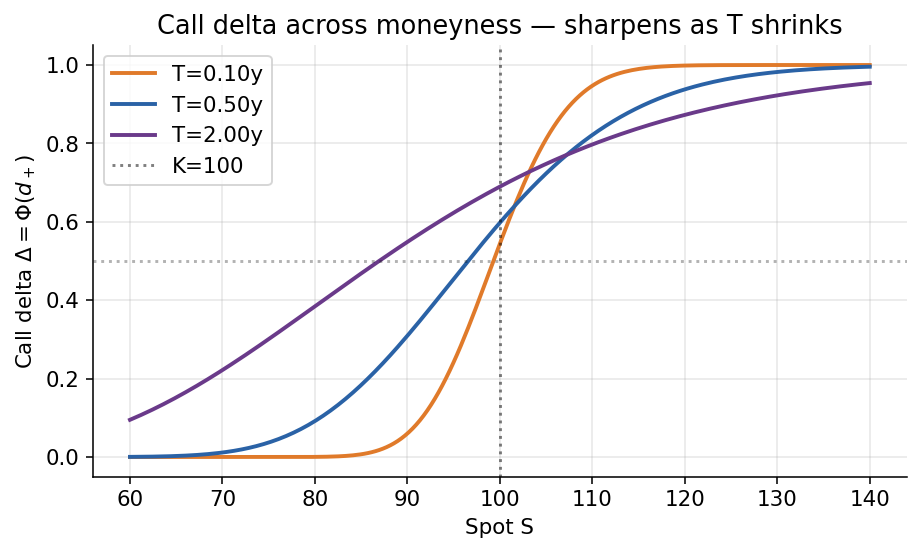
\includegraphics[keepaspectratio]{figures/ch07-delta-profile.png}}
\emph{Black-Scholes call delta \(\Phi(d_+)\) as a function of spot for
three maturities. Long-dated options have gradual deltas spread across
moneyness; near expiry the delta compresses toward a step at the strike,
tracking the digital payoff that \(\Delta_{\mathrm{call}}\) becomes in
the \(T\downarrow t\) limit.}

\pandocbounded{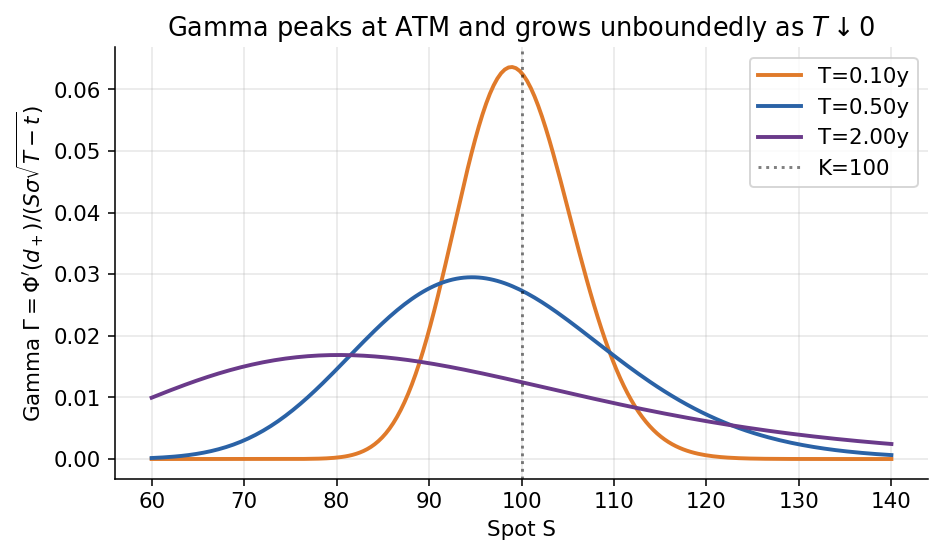
\includegraphics[keepaspectratio]{figures/ch07-gamma-vs-ttm.png}}
\emph{Gamma \(= \Phi'(d_+)/(S\sigma\sqrt{T-t})\) peaks at the
at-the-money strike for every maturity, and the peak grows without bound
as \(T\downarrow t\). A short ATM option is a short-gamma position that
becomes dangerously short as expiry approaches --- the terminal-gamma
pinning effect.}

\pandocbounded{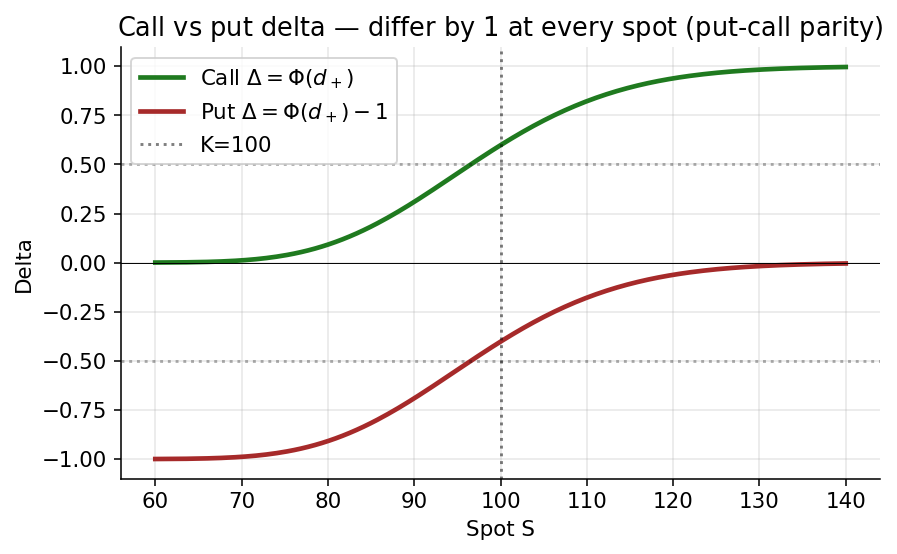
\includegraphics[keepaspectratio]{figures/ch07-call-put-delta.png}}
\emph{Put-call parity in delta form:
\(\Delta_{\mathrm{call}} - \Delta_{\mathrm{put}} = 1\) for every spot.
The call delta rises from \(0\) to \(+1\) through the strike; the put
delta sits a parallel unit below, running from \(-1\) to \(0\). A long
call plus a short put with the same strike is always \(100\%\) long the
underlying.}

Ch. 6's argument used one Greek (delta) because one Brownian was being
neutralised. A delta-hedged position is delta-hedged only at the
rebalance instant --- between rebalances, the residuals (gamma, vega,
etc.) are the dominant source of P\&L variance. A flow desk that leaves
gamma, vega, and dividends unmodelled isn't running a simplified BS
hedge --- it's running a book where residuals dominate. The residuals
are the business.

\begin{center}\rule{0.5\linewidth}{0.5pt}\end{center}

\section{7.2 Delta-gamma hedging --- two framings
unified}\label{delta-gamma-hedging-two-framings-unified}

A delta-neutral position is not risk-neutral: a \(\Delta S\) move costs
\(\tfrac12 \Gamma (\Delta S)^2\) --- for a short option, a guaranteed
loss on any move. To hedge gamma, add a second curved instrument
\(h(t, S_t)\) alongside the stock and cash. Two risky knobs
(\(\alpha_t\) shares, \(\gamma_t\) units of \(h\)) match two conditions:
delta and gamma.

Two framings give the same answer. \textbf{Framing A} (two-instrument
replication): match the target's \(\mathrm{d}W_t\) and \(\mathrm{d}t\)
coefficients. \textbf{Framing B} (local quadratic fit): match the first
two spatial derivatives via a \(2 \times 2\) linear system in
\((\alpha, \gamma)\) since stock has delta 1 and gamma 0, while \(h\)
has known \((\Delta^h, \Gamma^h)\).

\subsection{7.2.1 Local Taylor expansion of a
claim}\label{local-taylor-expansion-of-a-claim}

Second-order Taylor expansion of \(g(t, S)\) around \(S_t\):

\[
g(t, S) \;=\; g(t, S_t) \;+\; (S - S_t)\,\partial_S g(t, S_t)
\;+\; \tfrac{1}{2}\,(S - S_t)^2\,\partial_{SS} g(t, S_t) \;+\; \cdots, \tag{7.4}
\]

with the customary naming convention

\[
\Delta^g_t \;\equiv\; \partial_S g(t, S_t), \qquad
\Gamma^g_t \;\equiv\; \partial_{SS} g(t, S_t). \tag{7.5}
\]

Delta is slope, gamma is curvature. Geometrically: a delta-only hedge is
a tangent line; delta-gamma is a tangent parabola that hugs the payoff
over a wider window. Approximation error drops from \((\Delta S)^2\) to
\((\Delta S)^3\).

The quadratic truncation is natural under GBM:
\((\Delta S)^2 \sim S^2 \sigma^2 \Delta t\) is the same order as
\(\Delta t\), so it cannot be ignored without ignoring the PDE's
time-derivative structure. \((\Delta S)^3 \sim (\Delta t)^{3/2}\)
vanishes in the limit. Higher Greeks matter only through
discrete-rebalancing residuals.

\pandocbounded{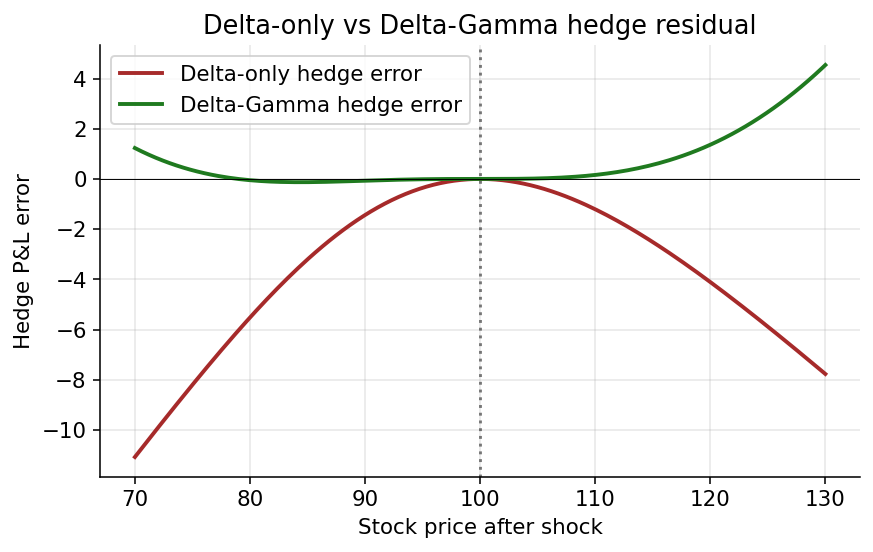
\includegraphics[keepaspectratio]{figures/ch07-dg-hedge.png}}
\emph{Figure 7.1 --- Delta-only hedge (tangent line) vs delta-gamma
hedge (tangent parabola) fit against the convex call payoff.}

\subsection{7.2.2 Framing A --- two-instrument
replication}\label{framing-a-two-instrument-replication}

We are short one unit of \(g\) and want a self-financing portfolio that
tracks it. Against a delta hedge alone, the \((\Delta S)^2\) residual
cannot be killed by a share position (stock has zero gamma) --- we need
a second curved instrument \(h\) with \(\partial_{SS} h \neq 0\).

Let \(h(t, S)\) be another traded option on \(S\) --- typically vanilla,
liquid, and chosen to have gamma at the same scale as the target's. The
hedging portfolio is

\[
V(t, S) \;=\; \alpha_t\,S \;+\; \beta_t\,M_t \;+\; \gamma_t\,h(t, S), \tag{7.6}
\]

where \(\alpha_t\) is the number of shares, \(\gamma_t\) is the number
of units of the auxiliary option, \(\beta_t\) is the number of units of
the money-market account \(M_t = e^{rt}\), and the hedge is set up so
that \(V\) matches the target \(g\) claim-for-claim. Applying a Taylor
expansion around \(S_t\) to both the portfolio and the target,

\[
V(t, S) \;=\; \alpha_t\,S \;+\; \beta_t\,M_t \;+\; \gamma_t\!\left[h(t, S_t)
+ (S - S_t)\,\partial_S h(t, S_t)
+ \tfrac{1}{2}(S - S_t)^2\,\partial_{SS} h(t, S_t)\right] + \cdots, \tag{7.7}
\]

\[
g(t, S) \;=\; g(t, S_t) \;+\; (S - S_t)\,\partial_S g(t, S_t)
\;+\; \tfrac{1}{2}(S - S_t)^2\,\partial_{SS} g(t, S_t) \;+\; \cdots. \tag{7.8}
\]

Matching coefficients of \((S - S_t)\) and \((S - S_t)^2\) between the
portfolio and the target gives the \emph{delta-gamma hedge conditions}:

\[
\alpha_t \;+\; \gamma_t\,\partial_S h(t, S_t) \;=\; \partial_S g(t, S_t), \tag{7.9}
\]

\[
\gamma_t\,\partial_{SS} h(t, S_t) \;=\; \partial_{SS} g(t, S_t). \tag{7.10}
\]

Denote \(\Delta^h_t = \partial_S h\), \(\Gamma^h_t = \partial_{SS} h\),
and \(\Delta^g_t\), \(\Gamma^g_t\) similarly. Solving (7.9)--(7.10) for
the two unknowns,

\[
\boxed{\;\gamma_t \;=\; \frac{\Gamma^g_t}{\Gamma^h_t}, \qquad
\alpha_t \;=\; \Delta^g_t \;-\; \frac{\Gamma^g_t}{\Gamma^h_t}\,\Delta^h_t. \;} \tag{7.11}
\]

These are the two hedge ratios. Read (7.11) as a two-step recipe: first
fix \(\gamma_t\) so that the auxiliary option's gamma times \(\gamma_t\)
matches the target gamma --- that is gamma-matching, equation (7.10);
then set \(\alpha_t\) so that the \emph{net} delta of the
\(\gamma_t\)-scaled auxiliary plus \(\alpha_t\)-scaled stock matches the
target delta --- that is delta-matching, equation (7.9), solved after
\(\gamma_t\) is pinned down. The order matters because gamma-matching
uses only \(h\) (the stock has zero gamma), while delta-matching uses
both \(h\) and \(S\). One cannot delta-hedge first and then gamma-hedge,
because the gamma-hedge step would disturb the delta that had already
been arranged. The correct order --- gamma first, then delta --- is the
operational lesson of the pair (7.11).

With \(\alpha_t\) and \(\gamma_t\) in hand, the cash leg follows from
the total portfolio value. At inception, we sold \(g\) and collected
\(g_0\); we bought \(\gamma_0\) units of \(h\) at \(h_0\) and
\(\alpha_0\) shares at \(S_0\); whatever is left we deposit in the bank,
so

\[
M_0 \;=\; g_0 \;-\; \alpha_0\,S_0 \;-\; \gamma_0\,h_0. \tag{7.12}
\]

This is the delta-gamma analogue of the delta-only initial-balance
recipe from §6.11.2: the premium collected pays for both the share-hedge
and the option-hedge, and the residual sits in the bank earning the
short rate. Depending on the sign of \(\gamma_0\) and the price of
\(h\), the initial bank balance may be positive (net lender) or negative
(net borrower). For a short position in a short-dated at-the-money call
hedged with a short-dated different-strike call, typically
\(\gamma_0 > 0\) (we are \emph{long} gamma in the auxiliary to offset
our \emph{short} gamma in the target), which means we pay for \(h\) and
the initial bank balance shrinks by \(\gamma_0 h_0\) relative to the
delta-only hedge.

Verifying that the resulting portfolio matches both delta and gamma is a
one-line check:

\[
\Delta^V_t \;=\; \alpha_t \;+\; \gamma_t\,\Delta^h_t \;=\; \Delta^g_t, \qquad
\Gamma^V_t \;=\; \gamma_t\,\Gamma^h_t \;=\; \Gamma^g_t. \tag{7.13}
\]

Both hold by construction. The portfolio tracks the target to second
order, and the tracking error is now of order \((S - S_t)^3\) rather
than \((S - S_t)^2\). Under a Brownian-motion underlying, the cubic term
is of order \((\Delta t)^{3/2}\) per rebalance interval, substantially
smaller than the \(\Delta t\) gamma residual of the delta-only hedge.
Delta-gamma hedging is therefore genuinely higher-order: it does not
merely shift the coefficient on the error, it shifts the \emph{scaling
exponent} --- the variance of the tracking error now falls as \(1/N^2\)
in the rebalance count rather than \(1/N\), and the standard deviation
falls as \(1/N\) rather than \(1/\sqrt{N}\).

The structural story is therefore clean. A delta-only hedge replicates
the target's Itô expansion only through the \(\mathrm{d}W\) coefficient;
the second-order \(\mathrm{d}t\) piece proportional to \(\Gamma\) is
unmatched. A delta-gamma hedge replicates \emph{both} coefficients, by
enlarging the hedging basis to include a second traded claim whose own
expansion has the required curvature. Each additional Greek matched
corresponds to one additional hedging instrument in the basis and one
additional linear equation to solve; the arithmetic remains elementary,
and the replication theorem of Chapter 6 generalises verbatim.

\subsection{7.2.3 Framing B --- local quadratic
fit}\label{framing-b-local-quadratic-fit}

The practical view starts from a slightly different position. A hedged
book has a \emph{loss distribution}, and the purpose of hedging is to
compress that distribution toward zero --- ideally a tight cluster
around a risk-free return but more realistically a tight cluster around
whatever expected alpha the strategy aims to extract. Delta hedging
collapses the linear dependence on the underlying; delta-gamma hedging
additionally collapses the quadratic dependence. Each additional Greek
matched corresponds to a further reduction in the variance of the hedged
P\&L --- and hence a smaller VaR and CTE at any confidence level.

The economic logic is worth stating plainly. When a derivatives dealer
sells an option, the premium received is --- in theory --- exactly the
expected discounted cost of replicating the option's payoff under a
specific hedging strategy. The hedging strategy itself is the
\emph{justification} for the premium: ``we charge \(g_0\) because if we
trade according to these rules, we can deliver \(\varphi(S_T)\) for
exactly \(g_0\) plus a small residual that vanishes in the limit of
continuous rebalancing --- the Black--Scholes promise.

Hedging exchanges one risk for another. Delta-only converts price risk
into gamma-residual risk; delta-gamma converts that into smaller
third-order residual plus model risk (gamma depends on \(\sigma\), which
may be mis-specified). The job is to hedge dangerous risks and leave
safe ones alone, not to hedge everything.

The Taylor expansion of \(g(t, S_t + \Delta S)\):

\[
g(t, S_t + \Delta S) \;=\; g(t, S_t)
\;+\; \Delta S\,\underbrace{\partial_S g(t, S_t)}_{\text{delta } \Delta}
\;+\; \tfrac{1}{2}(\Delta S)^2\,\underbrace{\partial_{SS} g(t, S_t)}_{\text{gamma } \Gamma}
\;+\; \cdots. \tag{7.14}
\]

Hedge a short position in \(g\) using \(S_t\), \(M_t\), and an auxiliary
\(h_t\). With \(\alpha_t\) shares, \(\beta_t\) cash, \(\gamma_t\) units
of \(h\):

\[
V_t \;=\; \alpha_t\,S_t \;+\; \beta_t\,M_t \;+\; \gamma_t\,h_t, \tag{7.15}
\]

and we \emph{fit} its spatial derivatives at \(S_t\) to those of the
target. The first-derivative match is

\[
\partial_S V_t \;=\; \alpha_t \;+\; \gamma_t\,\partial_S h \;=\; \Delta^g, \tag{7.16}
\]

and the second-derivative match is

\[
\partial_{SS} V_t \;=\; \gamma_t\,\partial_{SS} h \;=\; \Gamma^g, \tag{7.17}
\]

since stock and cash both contribute zero gamma; only \(h\) carries
curvature.

Matrix form:

\[
\begin{pmatrix} 1 & \Delta^h \\ 0 & \Gamma^h \end{pmatrix}
\begin{pmatrix} \alpha_t \\ \gamma_t \end{pmatrix}
\;=\;
\begin{pmatrix} \Delta^g \\ \Gamma^g \end{pmatrix}. \tag{7.18}
\]

Upper-triangular --- stock contributes only to delta. Inverting:

\[
\begin{pmatrix} \alpha_t \\ \gamma_t \end{pmatrix}
\;=\;
\begin{pmatrix} 1 & -\Delta^h/\Gamma^h \\ 0 & 1/\Gamma^h \end{pmatrix}
\begin{pmatrix} \Delta^g \\ \Gamma^g \end{pmatrix}, \tag{7.19}
\]

which recovers exactly the boxed pair from Framing A:

\[
\gamma_t \;=\; \frac{\Gamma^g}{\Gamma^h}, \qquad
\alpha_t \;=\; \Delta^g \;-\; \frac{\Gamma^g}{\Gamma^h}\,\Delta^h. \tag{7.20}
\]

\(h\) is almost always a liquid ATM short-dated vanilla --- high gamma
per dollar of premium, tight bid-ask, moderate turnover. Deep-ITM or
far-OTM hedges work mathematically but cost more (in notional, in
turnover, or in spread).

Matching multiple higher Greeks needs multiple auxiliary instruments;
serious exotic-hedging desks fit the target's Greek vector to the span
of dozens of liquid vanillas via least squares. Near-singular Greek
matrices (parallel hedges) need ridge regularisation or a more diverse
basis.

Common error: compute \(\alpha = \Delta^g\) and bolt on a gamma-hedge
--- internally inconsistent because \(h\) has its own delta. The correct
construction is simultaneous, as in (7.20).

\subsection{7.2.4 Reconciling the two
framings}\label{reconciling-the-two-framings}

Both framings give the same boxed hedge ratios. The duality: matching
Itô dynamics is matching the spatial Taylor expansion, in this
single-factor GBM setting. For smooth \(V(t, S_t)\), Itô gives

\[
\mathrm{d}V \;=\; \left(\partial_t V + \mu\,S_t\,\partial_S V + \tfrac{1}{2}\sigma^2 S_t^2\,\partial_{SS} V\right)\mathrm{d}t
\;+\; \sigma\,S_t\,\partial_S V\,\mathrm{d}W_t. \tag{7.21}
\]

The \(\mathrm{d}W_t\) coefficient is \(\sigma S_t \partial_S V\)
(delta); the \(\mathrm{d}t\)-coefficient buries \(\partial_{SS} V\) in
the convexity term. Matching delta and gamma matches both. The
\(\partial_t\) and \(\mu \partial_S\) pieces are absorbed by the pricing
PDE (paid for by the cash leg), reducing to two equations in two
unknowns.

Framing A: continuous-time hedge is exact (Itô dynamics match). Framing
B: discrete-rebalance residual scales as \((\Delta S)^3\), std-dev
scales as \(1/N\) rather than \(1/\sqrt{N}\) for delta-only. We use
Framing B's linear algebra below --- it generalises to \(n\)-Greek
hedging with \(n\) instruments.

\subsection{7.2.5 Worked numerical example --- gamma-matching an ATM
option}\label{worked-numerical-example-gamma-matching-an-atm-option}

Sell a 1-year ATM call (\(K_g = 100\), \(\sigma = 25\%\), \(r = 3\%\)):
\(g_0 \approx 10.94\), \(\Delta^g \approx 0.59\),
\(\Gamma^g \approx 0.0156\). Hedge with a 3-month ATM call:
\(h_0 \approx 5.40\), \(\Delta^h \approx 0.53\),
\(\Gamma^h \approx 0.0313\).

Applying (7.20),

\[
\gamma_0 \;=\; \frac{\Gamma^g}{\Gamma^h} \;=\; \frac{0.0156}{0.0313} \;\approx\; 0.498. \tag{7.22}
\]

Buy 0.498 units of the 3-month call for every short 1-year. Then

\[
\alpha_0 \;=\; \Delta^g \;-\; \frac{\Gamma^g}{\Gamma^h}\,\Delta^h
\;=\; 0.59 \;-\; 0.498 \cdot 0.53 \;\approx\; 0.326. \tag{7.23}
\]

Buy 0.326 shares. Initial hedge outlay:

\[
\alpha_0 \cdot S_0 \;+\; \gamma_0 \cdot h_0
\;=\; 0.326 \cdot 100 \;+\; 0.498 \cdot 5.40
\;=\; 32.6 \;+\; 2.69 \;=\; 35.29. \tag{7.24}
\]

Cash collected \(g_0 = 10.94\), so the bank starts at

\[
M_0 \;=\; g_0 \;-\; \alpha_0 S_0 \;-\; \gamma_0 h_0 \;=\; 10.94 \;-\; 35.29 \;=\; -24.35. \tag{7.25}
\]

Borrow \$24.35 to establish the hedge. A pure delta hedge would need
\(\$48.06\) of borrowing (0.59 shares); the gamma-hedging option
supplies some of the delta. Trade-off: less borrowing but the auxiliary
call ages, introducing its own theta/vega and rebalancing schedule.

A 1-month hedging call has gamma \(\approx 0.054\) --- fewer units
needed (\(\gamma_0 \approx 0.289\)) but faster turnover. Notional
efficiency vs rebalancing cost; desk policy resolves it.

Sanity check on local fit. For a 2\% move (\(\Delta S = 2\)), the true
call price change is \(\approx 1.15\), delta-only predicts 1.18,
delta-gamma 1.21. Both within a cent because the 1-year option has
modest gamma. At 10\% moves the gap between delta-only and delta-gamma
opens to several percent --- delta-gamma is a superb \emph{local} hedge
and mediocre \emph{global} one. For large moves gamma itself decays away
from the strike, so the quadratic extrapolation systematically
over-predicts; speed corrections (third-order) and full revaluation are
needed for VaR and 3--5 sigma stress.

\subsection{7.2.6 The discrete delta-gamma
recursion}\label{the-discrete-delta-gamma-recursion}

When continuous rebalancing is discretised, the analogue of the
delta-only cash-account recursion of §6.11 for the two-instrument hedge
is

\[
M_{t_k} \;=\; M_{t_{k-1}}\,e^{r\,\Delta t}
\;-\; (\alpha_{t_k} - \alpha_{t_{k-1}})\,S_{t_k}
\;-\; (\gamma_{t_k} - \gamma_{t_{k-1}})\,h_{t_k}, \tag{7.26}
\]

where each rebalance at time \(t_k\) requires buying or selling enough
stock to restore the delta match, \emph{and} enough of the auxiliary
option to restore the gamma match. Both trades are funded out of the
bank account (or deposited into it), and the bank grows between
rebalances at the risk-free rate. The structure is identical to the
pure-delta recursion but with an extra \(h\)-trading term on the
right-hand side. Transaction costs, if included, are simply summed over
the two legs --- we take up the details in §7.5.

Equation (7.26) is the operational engine of any delta-gamma hedging
program. Each morning (or each rebalance tick) the trader observes the
new stock price \(S_{t_k}\) and option price \(h_{t_k}\), recomputes the
desired hedge weights \(\alpha_{t_k}\) and \(\gamma_{t_k}\) from (7.20)
using the updated Greeks, and executes the increments
\(\alpha_{t_k} - \alpha_{t_{k-1}}\) in the stock and
\(\gamma_{t_k} - \gamma_{t_{k-1}}\) in the option. The cash flow from
these executions debits the bank account. Between rebalances the bank
account compounds at the short rate.

The \emph{absolute} size of each rebalance trade depends on how much the
Greeks have drifted since the last rebalance, which in turn depends on
how much the stock has moved, how much time has passed, and how curved
the target's Greek profile is. A near-the-money, short-dated option has
delta and gamma that change rapidly with spot, so its hedge rebalances
frequently and the cash account sees a lot of churn. A far-dated,
deep-in-the-money option has an almost linear payoff and a nearly
constant delta, so the hedge barely moves and rebalance costs are low.
These observations underpin the whole \emph{gamma scalping} school of
proprietary option trading: taking long-gamma positions on short-dated
ATMs and systematically extracting the rebalance cash-flow turnover as
P\&L, funded by theta decay.

One useful mental model of the rebalance cash flow is to think of it as
a \emph{betting ledger} between the desk and the market. Each morning,
the stock has moved; the desk's required delta has changed; the desk
executes the delta change at the current stock price; and that execution
booked a cash flow. If the stock moved up and the desk had to buy more
stock to re-hedge, the desk pays for stock at a higher price than
yesterday's average --- so the rebalance has a small negative cash flow
relative to zero. If the stock moved up and the desk had to sell stock
(long-gamma position), the desk receives cash at the higher price and
the rebalance has a positive cash flow. The aggregate pattern of
positive and negative rebalance cash flows over the option's life is
exactly the \emph{gamma P\&L}, and its magnitude is
\(\tfrac{1}{2} \Gamma (\Delta S)^2\) per rebalance, summed over all
rebalances, minus the theta bleed. This is the famous ``buy low, sell
high'' mechanism that underlies gamma scalping --- and its mirror image,
the ``sell high, buy low'' pain of being short gamma in a trending
market.

At maturity \(t_N = T\), the portfolio wealth owes the option payoff:

\[
P_N \;=\; M_{t_{N-1}}\,e^{r\,\Delta t}
\;+\; \alpha_{t_{N-1}}\,S_{t_N}
\;+\; \gamma_{t_{N-1}}\,h_{t_N}
\;-\; \varphi(S_{t_N}), \tag{7.27}
\]

and the expression in parentheses collapses, if the hedge tracked
perfectly, to \(\varphi(S_{t_N})\), leaving \(P_N = 0\). In a
well-specified model with no transaction costs and continuous
rebalancing, (7.27) is identically zero; in reality, it is a small
random variable whose distribution is tighter than the analogous
delta-only P\&L because the leading gamma error has been removed. We
quantify the tightening next.

\subsection{7.2.7 Terminal P\&L and residual
scaling}\label{terminal-pl-and-residual-scaling}

At expiry \(t_N = T\) we liquidate the hedge and deliver the claim
payoff \(\varphi(S_T)\). The realised profit-and-loss of the delta-gamma
hedged book is

\[
\boxed{\;\mathrm{P\&L} \;=\; M_{t_{N-1}}\,e^{r\,\Delta t}
\;+\; \alpha_{t_{N-1}}\,S_{t_N}
\;+\; \gamma_{t_{N-1}}\,h_{t_N}
\;-\; \varphi(S_{t_N}).\;} \tag{7.28}
\]

Under a continuous-time, frictionless, complete-market set-up this
quantity is identically zero; under discrete rebalancing it is a random
variable whose variance shrinks as the grid is refined. The delta-gamma
hedge has an order-of-magnitude smaller P\&L variance than a pure delta
hedge because it neutralises the quadratic term in the Taylor expansion
--- the leading residual is cubic in \(\Delta S\) rather than quadratic.

The \emph{scaling argument} is worth carrying through carefully, because
it is the quantitative payoff of all the extra machinery. A delta-only
hedge leaves a residual that is quadratic in the stock move per
rebalance interval. The variance of that residual scales as the variance
of \((\Delta S)^2\), which for GBM is of order
\((\sigma^2 \Delta t)^2 \cdot S^4\). Summing over \(N\) rebalance
intervals of length \(\Delta t = T/N\), the total residual variance
scales as

\[
N \cdot \Big(\sigma^2 \tfrac{T}{N}\Big)^{\!2}
\;=\; \frac{\sigma^4 T^2}{N}. \tag{7.29}
\]

The standard deviation therefore scales as \(1/\sqrt{N}\) --- slow
convergence. A delta-gamma hedge leaves a residual that is \emph{cubic}
in the stock move per interval. Its variance scales as the variance of
\((\Delta S)^3 \sim
S^6 \sigma^6 (\Delta t)^3\). Summing,

\[
N \cdot \Big(\sigma^6 \tfrac{T^3}{N^3}\Big)
\;=\; \frac{\sigma^6 T^3}{N^2}, \tag{7.30}
\]

with standard deviation scaling as \(1/N\). So on a weekly grid, the
delta-gamma standard deviation is a factor \(\sqrt{N}\) smaller than the
delta-only standard deviation; for \(N = 52\) weekly rebalances, that is
roughly a factor of \(7\) reduction. The difference between
\(1/\sqrt{N}\) and \(1/N\) convergence is the practical justification
for the extra hedging instrument.

\pandocbounded{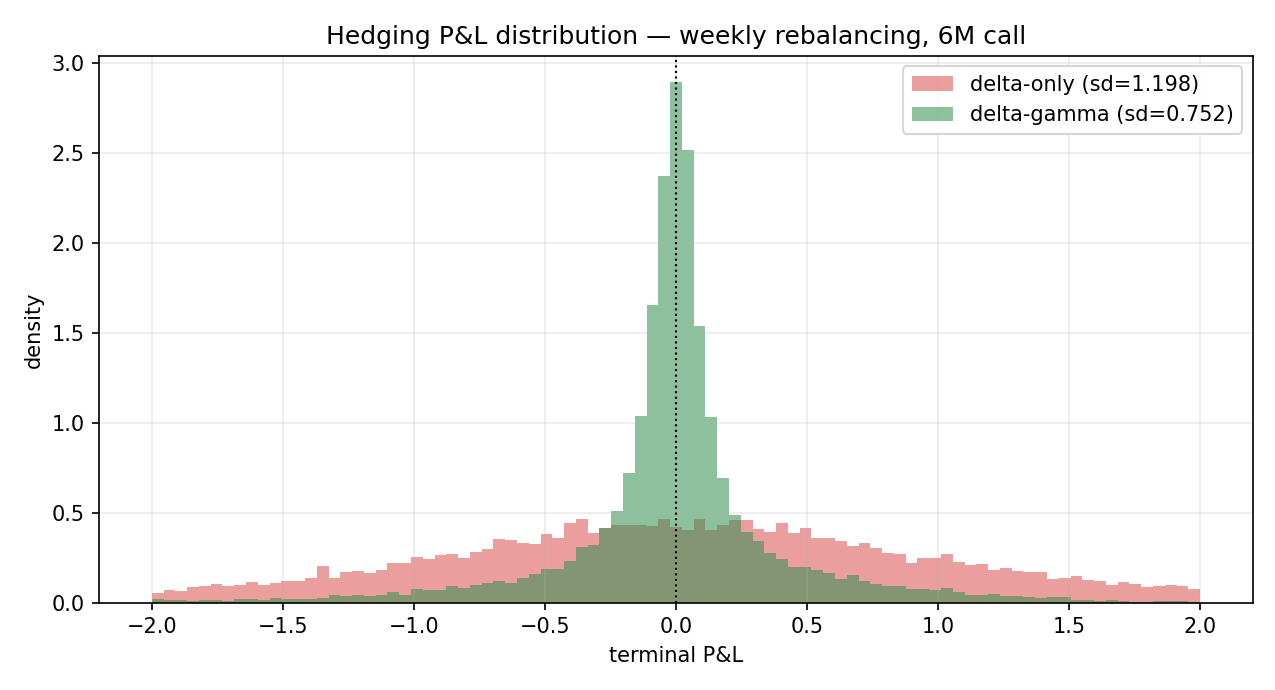
\includegraphics[keepaspectratio]{figures/ch07-hedge-pnl-density.png}}
\emph{Figure 7.2 --- Monte-Carlo terminal-P\&L density under weekly
rebalancing: delta-gamma hedge tightens variance by roughly \(2\times\)
relative to pure delta, with a tighter tail and lighter skew.}

The CTE-compression bonus is connected. Hedging reshapes the loss
distribution from chi-squared-heavy (delta-only, \((\Delta S)^2\)
residual) to near-Gaussian (delta-gamma, \((\Delta S)^3\) residual that
tends to cancel across rebalances), so the CTE of the hedged P\&L falls
by roughly the square of the factor by which the standard deviation
falls. Chapter 15 quantifies this and the Cornish-Fisher corrections it
implies.

\subsection{7.2.8 Trading the variance risk
premium}\label{trading-the-variance-risk-premium}

Pure delta hedging --- deliberately \emph{leaving} gamma exposure --- is
sometimes the trade, not a mistake. A long-gamma, delta-hedged option
position has P\&L over a small interval

\[
\Delta P \;\approx\; \tfrac{1}{2} \Gamma\,S^2\,\big(r_t^2 \;-\; \sigma_{\mathrm{imp}}^2\,\Delta t\big), \tag{7.31}
\]

where \(r_t\) is the realised log-return and \(\sigma_{\mathrm{imp}}\)
the implied vol the option was bought at. Aggregated over the option's
life, this is a \emph{realised-vs-implied variance} trade; its expected
P\&L is the \emph{variance risk premium} --- the systematic compensation
paid to long-vol traders for bearing the tail risk of vol spikes. In
equity-index options, implied exceeds realised by two to four points on
average, so short-vol (``gamma-scalping the short side'') earns small
consistent profits punctuated by catastrophic losses during spikes (Aug
2011, Feb 2018, Mar 2020). The choice between flattening gamma and
warehousing it is the difference between a flow desk (wants flat, books
bid-ask) and a vol desk (wants the exposure, monetises the VRP).

\subsection{7.2.9 Why two Greeks --- and why not
three?}\label{why-two-greeks-and-why-not-three}

Each additional Greek matched needs another liquid hedge with linearly
independent higher Greeks, and liquid markets supply a limited number.
The third-order Taylor term scales as
\((\Delta S)^3 \sim (\Delta t)^{3/2}\) --- small marginal variance
reduction per unit of hedging effort. Most desks stop at delta-gamma;
specialised books (vol-arb, barriers) add vega and sometimes
vanna/volga.

\emph{Speed} (\(\partial_{SSS} g\)) is the gamma of gamma; matching it
shaves another order off the residual variance but is rarely worth the
operational complexity. \emph{Colour} (\(\partial_{SSt} g\)) is gamma
decay; usually monitored, rarely hedged (just rebalance more frequently
near expiry).

Each business has a Greek fingerprint: FX desks emphasise vega/vanna,
equity-vol desks add volga, single-name desks add basis, rates-swaptions
desks add curve exposures.

\begin{center}\rule{0.5\linewidth}{0.5pt}\end{center}

\section{7.3 Vega and volatility risk}\label{vega-and-volatility-risk}

Vega is the option price's sensitivity to the volatility input:

\[
\mathcal{V}_t \;\equiv\; \partial_\sigma g(t, S_t;\, \sigma). \tag{7.32}
\]

Vega is the awkward first-order Greek because \(\sigma\) is not directly
traded --- only via variance swaps and VIX futures. (7.32)
differentiates a \emph{formula} with respect to a parameter, not a
market process; turning vega into a tradable hedge requires a
stochastic-vol model (§7.3.2).

\subsection{7.3.1 Vega of a vanilla Black-Scholes
call}\label{vega-of-a-vanilla-black-scholes-call}

For a European call under Black-Scholes, vega has a clean closed form,

\[
\mathcal{V}_t \;=\; S_t\,\sqrt{T - t}\,\Phi'(d_+), \tag{7.33}
\]

where
\(d_+ = [\ln(S_t/K) + (r + \tfrac{1}{2}\sigma^2)(T - t)] / (\sigma\sqrt{T-t})\)
is the usual moneyness index and \(\Phi'(x) = (2\pi)^{-1/2} e^{-x^2/2}\)
is the standard normal density. Two features of (7.33) are worth
flagging.

Vega is positive for every vanilla --- convex payoffs are monotone in
the spread of the underlying. Vega peaks ATM and decays to zero for deep
ITM or OTM. ATM short-dated has the most vega per dollar of premium;
deep-ITM LEAPS has essentially none.

\pandocbounded{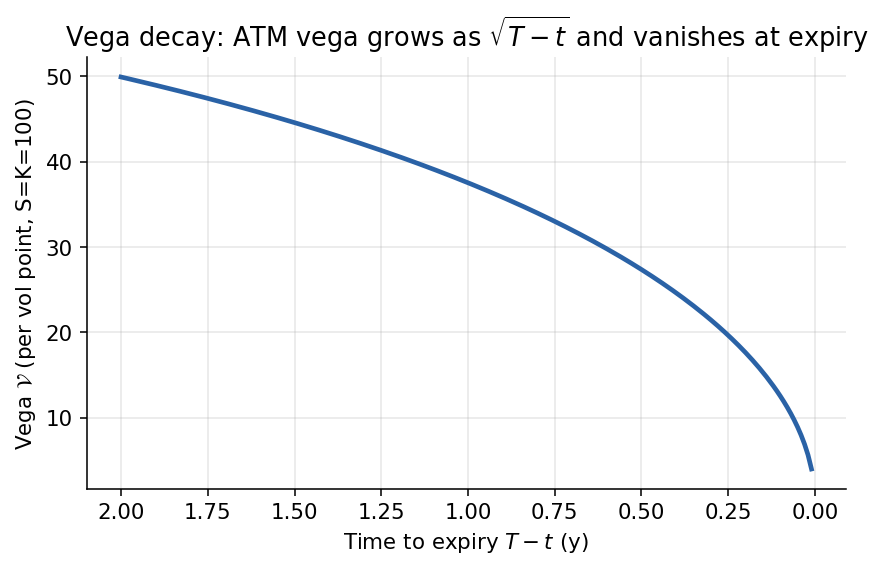
\includegraphics[keepaspectratio]{figures/ch07-vega-decay.png}}
\emph{ATM vega as a function of time-to-expiry (x-axis inverted so time
runs forward toward expiry on the right). Vega scales as \(\sqrt{T-t}\)
and collapses to zero at expiry --- the option has no volatility
sensitivity once the payoff is locked in. This is why short-dated ATM
options are the preferred instrument for }discharging* vega risk (low
cost per unit) and long-dated ATM options for \emph{accumulating} it.*

\pandocbounded{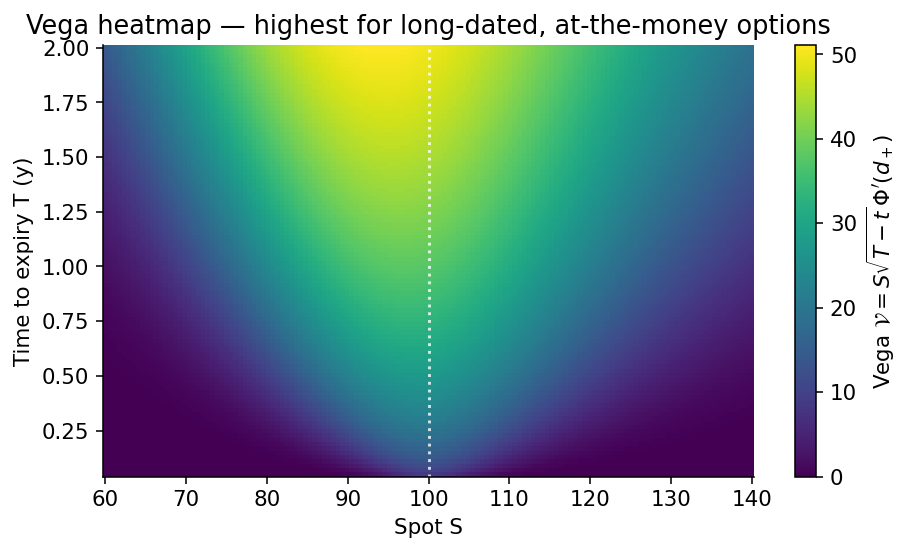
\includegraphics[keepaspectratio]{figures/ch07-vega-heatmap.png}}
\emph{Vega \(\mathcal{V} = S\sqrt{T-t}\,\Phi'(d_+)\) plotted over
\((S, T)\). The bright band runs along the at-the-money ridge; vega
grows with \(\sqrt{T-t}\) at fixed moneyness, so long-dated ATM options
carry the largest vega per contract. This is why ``volatility duration''
is a long-dated ATM product by construction.}

Straddles and strangles are the prototypical vol trades: max vega per
capital, near-zero delta by symmetry.

Numerical benchmark. At-the-money
\(\Phi'(0) = 1/\sqrt{2\pi} \approx 0.4\). For \(S = \$100\) and 3-month
expiry (\(\sqrt{0.25} = 0.5\)),

\[
\mathcal{V}_t \;\approx\; 100 \cdot 0.5 \cdot 0.4 \;=\; 20\text{ cents per volatility point}. \tag{7.34}
\]

A 1-point vol move costs the option 20 cents --- a substantial slice of
the premium. Vega is the second-largest P\&L source after directional
risk for most books.

\subsection{7.3.2 Volatility as a hidden state
variable}\label{volatility-as-a-hidden-state-variable}

Once \(\sigma\) becomes stochastic (Heston, SABR, local-vol --- Ch. 10),
the option price is \(g(t, S_t, \sigma_t)\) and Itô picks up extra
terms:

\[
\begin{aligned}
\mathrm{d}g_t \;=\;& \partial_t g\,\mathrm{d}t
\;+\; \partial_S g\,\mathrm{d}S_t
\;+\; \partial_\sigma g\,\mathrm{d}\sigma_t \\
&+\; \tfrac{1}{2}\partial_{SS} g\,\mathrm{d}\langle S, S\rangle_t
\;+\; \partial_{S\sigma} g\,\mathrm{d}\langle S, \sigma\rangle_t
\;+\; \tfrac{1}{2}\partial_{\sigma\sigma} g\,\mathrm{d}\langle \sigma, \sigma\rangle_t.
\end{aligned} \tag{7.35}
\]

The drift gains vega-times-drift-of-vol, vanna (\(\partial_{S\sigma}\),
cross-gamma), and volga (\(\partial_{\sigma\sigma}\)) pieces. A pure
delta hedge is no longer self-financing --- it leaks via vega and vanna
whenever \(\sigma\) moves. Closing the replication needs a second option
to match vega alongside delta-gamma. Real market-makers run a 2-D Greek
grid, not a single delta.

For three constraints (delta, gamma, vega) we need three hedging
instruments:

\[
\begin{pmatrix}
1 & \Delta^{h_1} & \Delta^{h_2} \\
0 & \Gamma^{h_1} & \Gamma^{h_2} \\
0 & \mathcal{V}^{h_1} & \mathcal{V}^{h_2}
\end{pmatrix}
\begin{pmatrix} \alpha_t \\ \gamma^1_t \\ \gamma^2_t \end{pmatrix}
\;=\;
\begin{pmatrix} \Delta^g \\ \Gamma^g \\ \mathcal{V}^g \end{pmatrix}, \tag{7.36}
\]

unique solution iff the \(2 \times 2\) sub-matrix in
\((\Gamma, \mathcal{V})\) is non-singular (i.e.~\(h_1\) and \(h_2\) have
linearly independent gamma-vega profiles). Dropping vega recovers
(7.20).

\subsection{7.3.3 Vega hedging in
practice}\label{vega-hedging-in-practice}

Desks track vega by tenor bucket --- front-month, second-month, etc. ---
because the implied-vol term structure can shift non-parallel. When
bucket vega exceeds its limit, the risk manager asks for an offset.

Calendar spreads (long short-dated straddle, short long-dated straddle)
produce near-vega-neutral positions whose \emph{term-structure} exposure
is the actual bet. Skew trades --- long OTM put, short OTM call (risk
reversal) --- are near-vega-neutral at ATM but heavy vanna; they
monetise skew steepening, the bread and butter of equity-index vol
desks.

Vega is a surface, not a number --- one vega per (strike, expiry). A
vega-neutral book has zero vega in every bucket.

\subsection{7.3.4 Higher-order volatility Greeks --- volga, vanna,
charm}\label{higher-order-volatility-greeks-volga-vanna-charm}

\emph{Volga} (\(\partial_{\sigma\sigma}\)), \emph{vanna}
(\(\partial_{S\sigma}\)), and \emph{charm} (\(\partial_{St}\)) matter
for structured-product desks (digitals, barriers, auto-callables,
cliquets).

\emph{Volga} is convexity in vol --- long-volga, vega-flat positions
profit when \(\sigma\) moves regardless of direction (a vol-of-vol bet).
Barriers and cliquets are volga-heavy near barriers; hedge with
butterflies.

\emph{Vanna} measures the cross-sensitivity of delta to volatility ---
or equivalently, the cross-sensitivity of vega to spot. A positive-vanna
position's delta increases when volatility rises; a negative-vanna
position's delta falls. Skew-sensitive structures (risk reversals, down-
and-out barriers) have concentrated vanna profiles, and hedging them
requires asymmetric choices of strikes --- typically out-of-the-money
puts and calls at different deltas to produce the desired vanna without
introducing vega or volga.

\emph{Charm} (or \(\partial \Delta / \partial t\)) measures how delta
drifts in time even when spot is constant. For an ATM short-dated call,
charm is small; for an in-the-money or out-of-the-money option near
expiry, charm can be substantial --- it is the source of ``delta decay''
that a trader sees as her book's delta drifts overnight even though
nothing in the market has moved. Charm is rarely hedged directly (since
time passes deterministically and more frequent delta-rebalancing
handles it), but it is prominently reported on overnight Greek sheets so
that the opening-book delta is correctly anticipated.

Each of these Greeks carries its own operational story, and each demands
a specific kind of hedging instrument to neutralise. The extension of
the replicating-portfolio argument to stochastic volatility, jumps, and
rough paths is the subject of entire later chapters (Chapter 10 for
Heston, beyond the present guide for jumps and rough vol) and is what
drives the ever-increasing complexity of modern derivatives-pricing
engines.

\begin{center}\rule{0.5\linewidth}{0.5pt}\end{center}

\section{7.4 Options on a dividend-paying
asset}\label{options-on-a-dividend-paying-asset}

The stock we have been hedging in Chapter 6 has paid no dividends --- it
is a ``pure capital appreciation'' asset, and its entire return has
flowed through the SDE
\(\mathrm{d}S_t / S_t = \mu\,\mathrm{d}t + \sigma\,
\mathrm{d}W_t\). Real stocks pay dividends, sometimes as quarterly cash
payouts, sometimes continuously (as in certain index products or in the
idealisation where we treat the total-return series). In the
continuous-dividend idealisation, the stock pays a dividend yield \(q\)
per unit time per unit of stock: an investor holding one share over
\([t, t + \mathrm{d}t]\) receives a cash payment \(q\,S_t\,\mathrm{d}t\)
into her account.

This small operational change propagates through the self-financing
replication argument in a specific and instructive way. The result is
the \emph{Black-Scholes-Merton PDE with dividend yield}, whose only
alteration from the no-dividend case is the replacement of \(r\) by
\(r - q\) in the drift coefficient of the first-derivative term.
Derivation follows.

\subsection{7.4.1 Setup --- continuous dividend
yield}\label{setup-continuous-dividend-yield}

Let \(S_t\) be the stock and let it satisfy

\[
\frac{\mathrm{d}S_t}{S_t} \;=\; \mu\,\mathrm{d}t \;+\; \sigma\,\mathrm{d}W_t, \tag{7.37}
\]

with a \emph{continuous dividend yield} \(q\): holding one share over
\([t, t + \mathrm{d}t]\) delivers \(q\,S_t\,\mathrm{d}t\) in cash. The
bank account is, as always,

\[
\mathrm{d}B_t \;=\; r\,B_t\,\mathrm{d}t. \tag{7.38}
\]

We value a European claim \(g_t = g(t, S_t)\) on \(S\) with terminal
payoff \(g(T, S) = \varphi(S)\). Writing \(g \in C^{1,2}\) so that Itô's
lemma applies, we set up a self-financing portfolio

\[
V_t \;=\; \alpha_t\,S_t \;+\; \beta_t\,B_t \;-\; g_t \tag{7.39}
\]

with \(\alpha_t\) shares, \(\beta_t\) units of cash, and a short unit of
the target claim. At inception we choose \(V_0 = 0\) --- the usual
replication convention.

\subsection{7.4.2 Self-financing increment with
dividends}\label{self-financing-increment-with-dividends}

The self-financing increment must now account for the dividend stream.
Over \([t, t + \mathrm{d}t]\) the wealth change has four sources: the
stock's price move \(\alpha_t\,\mathrm{d}S_t\), the dividend income
\(\alpha_t\,q\,S_t\,\mathrm{d}t\), the bank's growth
\(\beta_t\,\mathrm{d}B_t\), and the change in the short claim's value
\(-\mathrm{d}g_t\):

\[
\mathrm{d}V_t \;=\; \alpha_t\,\mathrm{d}S_t
\;+\; \alpha_t\,q\,S_t\,\mathrm{d}t
\;+\; \beta_t\,\mathrm{d}B_t
\;-\; \mathrm{d}g_t. \tag{7.40}
\]

The dividend term is what is new. Compared with the no-dividend setting,
(7.40) adds a positive drift \(\alpha_t\,q\,S_t\): shares held through
an interval earn a dividend whether or not the price moves. In the
stock-only part of the portfolio, this makes holding long \(\alpha_t\)
shares look more attractive than it did before --- an effect we will see
propagate into the option's PDE as a shift in the drift coefficient.

Expanding \(\mathrm{d}S_t\), \(\mathrm{d}B_t\), and \(\mathrm{d}g_t\)
via Itô's lemma,

\[
\mathrm{d}V_t \;=\; \alpha_t\!\left(\mu\,S_t\,\mathrm{d}t + \sigma\,S_t\,\mathrm{d}W_t\right)
\;+\; \alpha_t\,q\,S_t\,\mathrm{d}t
\;+\; \beta_t\,r\,B_t\,\mathrm{d}t
\;-\; \left[\big(\partial_t g + \mu\,S_t\,\partial_S g + \tfrac{1}{2}\sigma^2 S_t^2\,\partial_{SS} g\big)\mathrm{d}t
+ \sigma\,S_t\,\partial_S g\,\mathrm{d}W_t\right]. \tag{7.41}
\]

Grouping \(\mathrm{d}t\) and \(\mathrm{d}W\) separately,

\[
\mathrm{d}V_t \;=\;
\underbrace{\!\left[\alpha_t(\mu + q)S_t + \beta_t\,r\,B_t - \big(\partial_t g + \mu\,S_t\,\partial_S g + \tfrac{1}{2}\sigma^2 S_t^2\,\partial_{SS} g\big)\right]}_{\equiv\,\mathcal{A}_t}\!\mathrm{d}t
\;+\; \sigma\,S_t\!\left[\alpha_t - \partial_S g\right]\mathrm{d}W_t. \tag{7.42}
\]

\subsection{7.4.3 Zeroing the noise and
drift}\label{zeroing-the-noise-and-drift}

The coefficient of \(\mathrm{d}W_t\) in (7.42) vanishes iff

\[
\alpha_t \;=\; \partial_S g(t, S_t), \tag{7.43}
\]

which is the delta hedge --- identical to the no-dividend case. The
drift coefficient \(\mathcal{A}_t\) must vanish for \(V_t \equiv 0\) to
hold (since \(V_0 = 0\) and \(\mathrm{d}V_t\) must be predictable to
avoid an arbitrage). Setting \(\mathcal{A}_t = 0\) and substituting
\(\alpha_t = \partial_S g\),

\[
\partial_S g\,(\mu + q)\,S_t
\;+\; \beta_t\,r\,B_t
\;-\; \partial_t g
\;-\; \mu\,S_t\,\partial_S g
\;-\; \tfrac{1}{2}\sigma^2 S_t^2\,\partial_{SS} g \;=\; 0. \tag{7.44}
\]

The first and fourth terms combine:

\[
\partial_S g\,(\mu + q)\,S_t \;-\; \mu\,S_t\,\partial_S g \;=\; q\,S_t\,\partial_S g. \tag{7.45}
\]

Thus

\[
\beta_t\,r\,B_t \;=\; \partial_t g \;+\; \tfrac{1}{2}\sigma^2 S_t^2\,\partial_{SS} g \;-\; q\,S_t\,\partial_S g. \tag{7.46}
\]

\subsection{\texorpdfstring{7.4.4 Identifying \(\beta_t\) and closing
the
PDE}{7.4.4 Identifying \textbackslash beta\_t and closing the PDE}}\label{identifying-beta_t-and-closing-the-pde}

From \(V_t = 0\) and \(\alpha_t = \partial_S g\) we obtain

\[
\beta_t\,B_t \;=\; g_t \;-\; \alpha_t\,S_t \;=\; g_t \;-\; S_t\,\partial_S g. \tag{7.47}
\]

Substituting this into the left side of (7.46),

\[
r\,(g_t - S_t\,\partial_S g) \;=\; \partial_t g \;+\; \tfrac{1}{2}\sigma^2 S_t^2\,\partial_{SS} g \;-\; q\,S_t\,\partial_S g. \tag{7.48}
\]

Rearranging produces the \emph{Black-Scholes-Merton PDE with continuous
dividend yield}:

\[
\boxed{\;\partial_t g \;+\; (r - q)\,S\,\partial_S g \;+\; \tfrac{1}{2}\sigma^2 S^2\,\partial_{SS} g \;=\; r\,g,
\qquad g(T, S) = \varphi(S). \;} \tag{7.49}
\]

Compare with the no-dividend PDE of Chapter 6: the only change is that
the drift of the first-derivative term has become \(r - q\) rather than
\(r\). The discount rate on the right-hand side is still the full \(r\)
(the option itself does not pay a dividend), but the \emph{risk-neutral}
drift of the stock has been reduced by the dividend yield. Under the
risk-neutral measure \(\mathbb{Q}\), the stock now satisfies

\[
\mathrm{d}S_t \;=\; (r - q)\,S_t\,\mathrm{d}t \;+\; \sigma\,S_t\,\mathrm{d}\widehat{W}_t, \tag{7.50}
\]

so the \emph{total-return} process \(S_t e^{q t}\) (stock plus
reinvested dividends) drifts at \(r\), but the bare price process
\(S_t\) drifts at \(r - q\). The market is still risk-neutral on the
\emph{reinvestment} of dividends, but the quoted price lags the
reinvested total return by the dividend yield.

\(q = 0\) recovers Ch. 6's PDE --- the dividend correction enters the
drift only.

\subsection{7.4.5 The Black-Scholes-Merton formula with
dividends}\label{the-black-scholes-merton-formula-with-dividends}

The closed-form European call on a dividend-paying stock under (7.49) is

\[
g(t, S) \;=\; S\,e^{-q(T - t)}\,\Phi(d_+) \;-\; K\,e^{-r(T - t)}\,\Phi(d_-), \tag{7.51}
\]

with

\[
d_\pm \;=\; \frac{\ln(S/K) \;+\; \big(r - q \pm \tfrac{1}{2}\sigma^2\big)(T - t)}{\sigma\sqrt{T - t}}. \tag{7.52}
\]

Three features. The stock term carries \(e^{-q(T-t)}\) --- the option
holder doesn't receive dividends, so the effective stock value is
\(S e^{-q(T-t)}\). The moneyness drift becomes \(r - q\) relative to the
forward \(F_t = S_t e^{(r-q)(T-t)}\). Setting \(q = 0\) recovers Ch. 6;
treating \(K\) as a stochastic asset's ``self-dividend'' recovers
Margrabe (Ch. 8).

For a European put, the analogous formula is

\[
g(t, S) \;=\; K\,e^{-r(T-t)}\,\Phi(-d_-) \;-\; S\,e^{-q(T-t)}\,\Phi(-d_+), \tag{7.53}
\]

with the same \(d_\pm\) as the call --- a direct consequence of put-call
parity, which we state formally in §7.6.5.

Reinterpret via the forward \(F_t = S_t e^{(r-q)(T-t)}\):

\[
F_t \;=\; S_t\,e^{(r - q)(T - t)}, \tag{7.54}
\]

\[
g(t, S) \;=\; e^{-r(T-t)}\!\left[F_t\,\Phi(d_+) \;-\; K\,\Phi(d_-)\right], \tag{7.55}
\]

--- the classical formula with spot replaced by forward. Pricing against
the forward numeraire absorbs the dividend yield (Ch. 8).

\subsection{7.4.6 Delta of a dividend-paying
call}\label{delta-of-a-dividend-paying-call}

Differentiating (7.51) with respect to \(S\) gives

\[
\Delta_t \;=\; e^{-q(T - t)}\,\Phi(d_+). \tag{7.56}
\]

The \(e^{-q(T-t)}\) factor shrinks the delta vs the no-dividend case ---
a 2\% yield over 5y shaves the delta by \textasciitilde10\%. Traders who
ignore dividends overhedge and bleed P\&L.

The gamma is similarly modified:

\[
\Gamma_t \;=\; \frac{e^{-q(T - t)}\,\Phi'(d_+)}{S\,\sigma\sqrt{T - t}}, \tag{7.57}
\]

and the vega is

\[
\mathcal{V}_t \;=\; S\,e^{-q(T - t)}\,\sqrt{T - t}\,\Phi'(d_+). \tag{7.58}
\]

An equivalent \(K\)-form via
\(S e^{-q(T-t)} \Phi'(d_+) = K e^{-r(T-t)} \Phi'(d_-)\) gives
\(\mathcal{V}_t = K e^{-r(T-t)} \sqrt{T-t} \Phi'(d_-)\).

The \(S\)-leg always carries \(e^{-q(T-t)}\); the \(K\)-leg always
carries \(e^{-r(T-t)}\). A library returning the no-dividend delta on a
dividend stock is wrong.

\subsection{7.4.7 Forward reformulation}\label{forward-reformulation}

The cleanest route on dividend-paying stocks is via the forward \(F_t\)
of (7.54), a \(\mathbb{Q}\)-martingale:

\[
g(t, F) \;=\; e^{-r(T - t)}\,\mathbb{E}^{\mathbb{Q}}_t[\varphi(F_T)], \tag{7.59}
\]

For \(\varphi(F) = (F - K)_+\) this evaluates to (7.55) --- Black-76,
which reappears in Ch. 8, 13, and 14 with only the definition of ``the
forward'' changing. \emph{Dividends tilt the drift; they do not change
the structure.}

\begin{center}\rule{0.5\linewidth}{0.5pt}\end{center}

\section{7.5 Transaction costs and the self-financing
bookkeeping}\label{transaction-costs-and-the-self-financing-bookkeeping}

Self-financing intuitively says no external cash flows. But adjusting
weights \((\alpha_t, \beta_t, \gamma_t)\) creates price-driven cash
flows, and the naive
``\(\mathrm{d}V = \alpha\,\mathrm{d}S + \beta\,\mathrm{d}M\)'' only
holds with the right covariation bookkeeping. Ch. 6 elided this; we
revisit it here to handle transaction costs and stochastic hedge
weights.

\subsection{7.5.1 Self-financing revisited --- the covariation
terms}\label{self-financing-revisited-the-covariation-terms}

For a portfolio \(V_t = \alpha_t\,S_t + \beta_t\,M_t - g_t\) (long
stock, long cash, short the claim we sold), Itô's product rule gives

\[
\begin{aligned}
\mathrm{d}V_t \;=\;& \alpha_t\,\mathrm{d}S_t \;+\; \beta_t\,\mathrm{d}M_t \;-\; \mathrm{d}g_t \\
&+\; \mathrm{d}\alpha_t\,S_t \;+\; \mathrm{d}\beta_t\,M_t \;+\; \mathrm{d}[\alpha, S]_t \;+\; \mathrm{d}[\beta, M]_t.
\end{aligned} \tag{7.60}
\]

Gain-from-trading:
\(\alpha_t\,\mathrm{d}S_t + \beta_t\,\mathrm{d}M_t - \mathrm{d}g_t\).
The remaining four terms (rebalance + covariation) must vanish under
self-financing. Since \((\alpha_t, \beta_t)\) are stochastic and adapted
to \(S\), the covariations \(\mathrm{d}[\alpha, S]\) are non-zero in any
real hedging context.

\subsection{7.5.2 Before-and-after rebalance
accounting}\label{before-and-after-rebalance-accounting}

Fix the instant \(t\) and split it into a before-rebalance leg using
\((\alpha_t, \beta_t)\) and an after-rebalance leg using
\((\alpha_{t + \Delta t},
\beta_{t + \Delta t})\). The before-leg value carried into
\(t + \Delta t\) is

\[
\alpha_t\,S_{t + \Delta t} \;+\; \beta_t\,M_{t + \Delta t} \;-\; g_{t + \Delta t}, \tag{7.61}
\]

and the after-leg value at \(t + \Delta t\) is

\[
\alpha_{t + \Delta t}\,S_{t + \Delta t} \;+\; \beta_{t + \Delta t}\,M_{t + \Delta t} \;-\; g_{t + \Delta t}. \tag{7.62}
\]

The discrete value increment

\[
\Delta V_t \;=\; \alpha_t\,\Delta S_t \;+\; \beta_t\,\Delta M_t \;-\; \Delta g_t \tag{7.63}
\]

is valid only if before \(=\) after at \(t + \Delta t\), i.e.

\[
\Delta\alpha_t\,\underbrace{S_{t + \Delta t}}_{S_t + \Delta S_t}
\;+\; \Delta\beta_t\,\underbrace{M_{t + \Delta t}}_{M_t + \Delta M_t} \;=\; 0. \tag{7.64}
\]

Expanding the product,

\[
\Delta\alpha_t\,S_t \;+\; \Delta\alpha_t\,\Delta S_t \;+\; \Delta\beta_t\,M_t \;+\; \Delta\beta_t\,\Delta M_t \;=\; 0, \tag{7.65}
\]

and passing to the continuous limit (where \(\Delta\alpha\,\Delta S \to
\mathrm{d}[\alpha, S]\), the quadratic covariation),

\[
\boxed{\;\mathrm{d}\alpha_t\,S_t \;+\; \mathrm{d}[\alpha, S]_t \;+\; \mathrm{d}\beta_t\,M_t \;+\; \mathrm{d}[\beta, M]_t \;=\; 0.\;} \tag{7.66}
\]

(7.66) is self-financing in precise form: writing
``\(\mathrm{d}V = \alpha\,\mathrm{d}S + \beta\,\mathrm{d}M\)'' assumes
(7.66) as a side condition, not automatic.

For \(\alpha = \Delta(t, S_t)\), Itô gives

\[
\mathrm{d}[\alpha, S]_t \;=\; \partial_S \Delta\,\mathrm{d}[S, S]_t
\;=\; \Gamma\,\sigma^2 S^2\,\mathrm{d}t \tag{7.67}
\]

--- the gamma-variance bleed at the heart of option theory. The
\(\tfrac12 \sigma^2 S^2 \partial_{SS}\) term in the BS PDE comes
directly from this covariation.

\subsection{7.5.3 Proportional transaction
costs}\label{proportional-transaction-costs}

A rebalance of size \(\Delta\alpha_t\) costs
\(c|\Delta\alpha_t| S_{t+\Delta t}\) for a proportional spread \(c\).
Self-financing picks up a negative term:

\[
\mathrm{d}\alpha_t\,S_t \;+\; \mathrm{d}[\alpha, S]_t
\;+\; \mathrm{d}\beta_t\,M_t \;+\; \mathrm{d}[\beta, M]_t
\;=\; -c\,|\mathrm{d}\alpha_t|\,S_t \;-\; c\,|\mathrm{d}\gamma_t|\,h_t. \tag{7.68}
\]

The absolute value matters: cost is paid on every trade, so it doesn't
cancel across oscillating rebalances. This drives the
optimal-hedging-band framework (Davis--Norman, Whalley--Wilmott) ---
defer rebalances until delta drift exceeds a cost-vol threshold.

To get a sense of the magnitude, suppose a desk is delta-hedging a
single option over a year, with daily rebalances (so \(N = 250\)). For
an ATM three-month call on a \(\$100\) stock with \(\sigma = 25\%\), the
typical daily \(|\Delta\alpha_t|\) is of order
\(\Gamma \cdot |\Delta S| \approx 0.032 \cdot
(100 \cdot 0.25/\sqrt{250}) \approx 0.05\) shares per day. With a
bid-ask spread of \(c = 0.01\%\) (one basis point --- typical for listed
equity), the daily cost is \(0.01\% \cdot 0.05 \cdot 100 = \$0.0005\)
per option. Over \(250\) days, the cumulative cost is about \(\$0.12\)
per option, or roughly \(1\%\) of the option's premium --- small but not
negligible. For illiquid or wide-spread markets (\(c = 0.1\%\) or
higher), the cumulative cost can be several percent of the premium,
which fundamentally changes the economics of the trade.

A gamma hedge using an option with wide bid-ask can cost more than the
gamma reduction is worth --- pure-delta then wins. Delta-gamma is
justified only when the auxiliary option's spread is small relative to
the variance saving.

\subsection{7.5.4 Leland volatility
adjustment}\label{leland-volatility-adjustment}

Under proportional costs the dealer prices the option as if vol were
slightly higher:

\[
\sigma_{\mathrm{Leland}}^{\,2} \;=\; \sigma^2 \;+\; c\,\sigma\,\sqrt{\frac{8}{\pi\,\Delta t}}, \tag{7.69}
\]

with \(\Delta t\) the rebalance interval and \(c\) the proportional
bid-ask. At \(c = 0.01\%\), daily rebalancing (\(\Delta t = 1/250\)),
and \(\sigma =
25\%\), the adjustment is \(\approx 0.006\), i.e.~\(\approx 0.6\) vol
points; at \(c = 0.1\%\) (stressed) it jumps to \(\approx 6\) points.
Real dealer prices overlay (7.69) plus XVA, skew, and liquidity premia
onto the textbook \(\sigma\).

\begin{center}\rule{0.5\linewidth}{0.5pt}\end{center}

\section{7.6 Put-call parity, deltas, and
gammas}\label{put-call-parity-deltas-and-gammas}

Throughout this section \(C = C(t, S)\) and \(P = P(t, S)\) denote the
Black-Scholes European call and put prices on a stock paying a
continuous dividend yield \(q\), struck at \(K\) and expiring at \(T\);
we write \(\tau = T - t\) for time to expiry. The one identity that ties
them together is put-call parity,

\[
C(t, S) \;-\; P(t, S) \;=\; S\,e^{-q\tau} \;-\; K\,e^{-r\tau}. \tag{7.70}
\]

(7.70) is a static, \emph{model-independent} identity: it is a
no-arbitrage consequence of the trivial payoff decomposition
\(\max(S_T - K, 0) - \max(K - S_T, 0) = S_T - K\), discounted to \(t\).
Every Greek identity between call and put follows by differentiating
(7.70) in the relevant variable --- spot, volatility, time, or rate ---
and the right-hand side, which is a simple forward contract minus a
zero-coupon bond, is transparent in each.

\subsection{7.6.1 Put price curve}\label{put-price-curve}

Applying parity to the call formula (7.51) gives the closed-form put
price under continuous dividend yield:

\[
P(t, S) \;=\; K\,e^{-r\tau}\,\Phi(-d_-) \;-\; S\,e^{-q\tau}\,\Phi(-d_+), \tag{7.71}
\]

with \(d_\pm\) as in (7.52). The put is convex in \(S\), monotonically
decreasing (a larger spot lowers the value of the right-to-sell), and
tends to \(K e^{-r\tau} - S e^{-q\tau}\) deep in the money (\(S \ll K\))
and to \(0\) deep out of the money (\(S \gg K\)). At expiry the curve
collapses to the hockey-stick payoff \(\max(K - S_T, 0)\).

\subsection{7.6.2 Call price curve}\label{call-price-curve}

For reference alongside (7.71) the call price (7.51) is

\[
C(t, S) \;=\; S\,e^{-q\tau}\,\Phi(d_+) \;-\; K\,e^{-r\tau}\,\Phi(d_-). \tag{7.72}
\]

The call is convex in \(S\), monotonically increasing, bounded below by
the intrinsic value \((S e^{-q\tau} - K e^{-r\tau})_+\) (the modified
forward-minus-bond) and above by \(S e^{-q\tau}\).

\subsection{7.6.3 Delta curves}\label{delta-curves}

Differentiating (7.70) once in \(S\) and using
\(\partial_S(S e^{-q\tau}) = e^{-q\tau}\) gives the \emph{parity
identity for delta},

\[
\Delta^C \;-\; \Delta^P \;=\; e^{-q\tau}. \tag{7.73}
\]

Combined with the call-delta formula \(\Delta^C = e^{-q\tau}\Phi(d_+)\)
from (7.56), this yields the put delta

\[
\Delta^P \;=\; e^{-q\tau}\Phi(d_+) \;-\; e^{-q\tau} \;=\; -\,e^{-q\tau}\,\Phi(-d_+). \tag{7.74}
\]

As expected, \(\Delta^P \in [-e^{-q\tau}, 0]\): a long put has negative
delta bounded below by \(-e^{-q\tau}\) (ATM-deep-ITM put \(\to\) near
\(-e^{-q\tau}\); OTM put \(\to 0\)). The two delta curves are vertical
translates of each other by \(e^{-q\tau}\) --- a clean visual
diagnostic.

\subsection{7.6.4 Gamma curves and pin
risk}\label{gamma-curves-and-pin-risk}

Differentiating (7.73) once more in \(S\), the right-hand side
\(e^{-q\tau}\) is constant in \(S\), so

\[
\Gamma^C \;=\; \Gamma^P \;=\; \frac{e^{-q\tau}\,\Phi'(d_+)}{S\,\sigma\sqrt{\tau}}. \tag{7.75}
\]

This is the \emph{gamma parity identity} previewed in §7.1 --- calls and
puts at the same strike share a single gamma curve. Consequently, a
delta-neutral spread that is short one call and long one put at the same
strike has \emph{zero} gamma; the combination is the synthetic short
forward of §7.6.6, whose value is linear in \(S\).

\emph{Pin risk.} As \(\tau \downarrow 0\) the ATM gamma blows up like
\(1/\sqrt{\tau}\): from (7.75) at \(S = K e^{(r-q)\tau}\),
\(\Gamma \sim 1/(K\sigma\sqrt{2\pi\tau})\). A short ATM option on expiry
day can whip between \(\Delta = 0\) and \(\Delta = \pm e^{-q\tau}\) as
\(S\) crosses \(K\) --- the delta becomes a step function and hedging it
requires arbitrarily-large trades on arbitrarily-small spot moves. This
is \emph{pin risk}. Because \(\Gamma^C = \Gamma^P\), it afflicts calls
and puts symmetrically, and it is one of the main reasons market makers
flatten ATM option exposure in the final hours before expiry.

\subsection{7.6.5 Put-call parity and its Greek
consequences}\label{put-call-parity-and-its-greek-consequences}

We now collect the full slate of parity consequences obtained by
differentiating (7.70) in each model variable. All follow mechanically,
and the right-hand side of each identity has a transparent
forward-minus-bond interpretation.

\textbf{Delta.} \(\partial_S\) of (7.70):
\(\Delta^C - \Delta^P = e^{-q\tau}\). (7.73)

\textbf{Gamma.} \(\partial_{SS}\) of (7.70): \(\Gamma^C = \Gamma^P\).
(7.75) The right-hand side of parity is linear in \(S\), so its second
derivative vanishes.

\textbf{Vega.} Neither \(S e^{-q\tau}\) nor \(K e^{-r\tau}\) depends on
\(\sigma\) (parity is a \emph{static} no-arb identity independent of
volatility assumptions), so \(\partial_\sigma\) of (7.70) gives

\[
\mathcal{V}^C \;=\; \mathcal{V}^P. \tag{7.76}
\]

Calls and puts at the same strike share a single vega curve. A
delta-hedged short call is vega-short; a delta-hedged short put is
equally vega-short --- which is why a straddle (long call + long put at
the same strike) doubles vega, matching (7.76) with a factor of two.

\textbf{Theta.} \(\partial_t\) of (7.70), using
\(\partial_t e^{-q\tau} =
q e^{-q\tau}\) and \(\partial_t e^{-r\tau} = r e^{-r\tau}\):

\[
\Theta^C \;-\; \Theta^P \;=\; -\,q\,S\,e^{-q\tau} \;+\; r\,K\,e^{-r\tau}. \tag{7.77}
\]

The difference in theta is \emph{not} zero, because the forward and the
bond on the right-hand side of parity each decay at their own rate. For
\(q = 0\) (no dividend), \(\Theta^C - \Theta^P = r K e^{-r\tau} > 0\),
so a call decays less unfavourably than a put of the same strike --- the
standard ``rates help calls, hurt puts'' intuition.

\textbf{Rho.} \(\partial_r\) of (7.70), noting that \(S e^{-q\tau}\) is
rate-independent while \(K e^{-r\tau}\) carries a \(-\tau\):

\[
\rho^C \;-\; \rho^P \;=\; \tau\,K\,e^{-r\tau}. \tag{7.78}
\]

Calls have positive rho and puts negative rho; the gap between them is
exactly the PV01-scale of the strike-bond.

\textbf{Dividend sensitivity.} \(\partial_q\) of (7.70):
\(\partial_q C - \partial_q P = -\tau S e^{-q\tau}\). Calls are hurt by
higher dividends (stock trades ex-div), puts benefit symmetrically.

These identities are all \emph{exact} and \emph{model-free} in the sense
that they follow from (7.70) without reference to any Black-Scholes or
log-normal assumption. They therefore hold in Heston, in local-vol, in
every complete arbitrage-free model --- any model in which parity is
imposed (which is every sensible model) respects (7.73)-(7.78)
identically.

\subsection{7.6.6 Synthetic positions}\label{synthetic-positions}

Rewriting parity as

\[
C \;-\; P \;=\; S\,e^{-q\tau} \;-\; K\,e^{-r\tau} \tag{7.79}
\]

says that a \emph{long-call-short-put} portfolio at strike \(K\) is
equivalent to a long position in \(e^{-q\tau}\) shares of stock
(equivalently, one forward contract delivered at \(T\)) funded by a
short \(K\)-notional zero-coupon bond maturing at \(T\). This is the
\emph{synthetic forward}: a way to construct directional equity exposure
from options alone.

Symmetric rearrangements give the other useful syntheses: synthetic long
stock is \(S e^{-q\tau} = C - P + K e^{-r\tau}\) (long call + short put
+ long bond); synthetic short stock is
\(-S e^{-q\tau} = P - C - K e^{-r\tau}\). Traders use these replications
when the physical stock is hard to borrow, when margin requirements
differ between cash equities and options, or when the options market is
more liquid than the stock at the relevant size. The Greek profile of a
synthetic is dictated by (7.73)-(7.78): a synthetic long forward is
delta-\(e^{-q\tau}\), gamma-zero, vega-zero, and
theta-\((-qSe^{-q\tau} + rKe^{-r\tau})\), which is exactly the Greek
profile of the forward contract it replicates --- a consistency check
with nothing to tune.

\begin{center}\rule{0.5\linewidth}{0.5pt}\end{center}

\section{7.7 Greek Visual Atlas}\label{greek-visual-atlas}

The closed-form expressions of §§7.1--7.6 capture the algebra of each
Greek; the pictures below capture the \emph{shape}. For a senior risk
manager the shape is what's load-bearing --- it is the shape that tells
you which strike will pin, which vega bucket will blow up under a vol
shock, and where the second-order risk lives that a delta hedger cannot
see. Every figure in this atlas is generated under the same flat
Black-Scholes world: \(S_0=K=100\), \(r=4\%\), \(q=0\), \(\sigma=25\%\),
with maturity slices \(T\in\{1\text{m}, 3\text{m},
12\text{m}\}\) unless the figure is specifically about expiry-day
effects.

\subsection{7.7.1 Theta --- the cost of
waiting}\label{theta-the-cost-of-waiting}

\begin{figure}
\centering
\pandocbounded{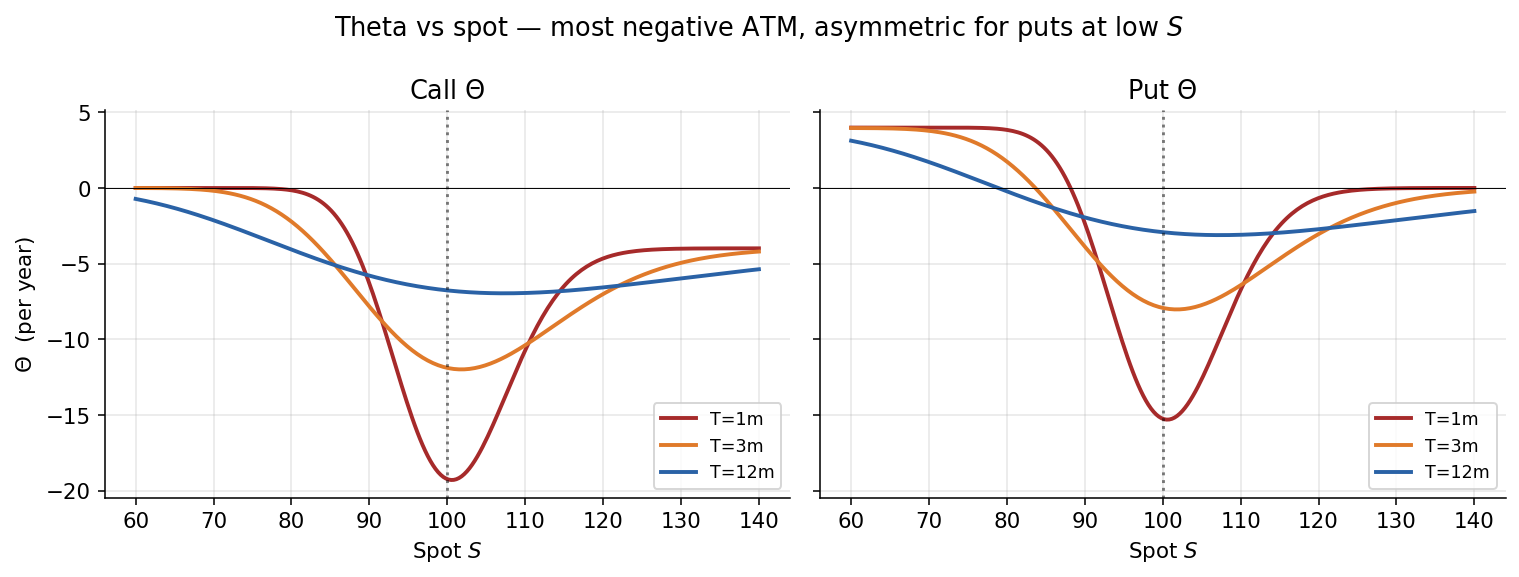
\includegraphics[keepaspectratio]{figures/ch07-theta-vs-spot.png}}
\caption{Theta vs spot for calls and puts, three TTMs}
\end{figure}

\emph{Call (left) and put (right) theta as a function of spot, at
\(T=1\)m, \(3\)m, \(12\)m.}

Theta is most negative right at the strike --- that is where convex
optionality is densest, so the time-decay charge per day is the largest.
The decay accelerates as expiry approaches: the \(1\)-month curve is
roughly three times deeper than the \(12\)-month curve. Note the
put-call asymmetry at low spot: the \(rKe^{-r\tau}\Phi(\pm d_-)\)
discount-funding term flips sign between (7.77)'s call and put forms, so
deep ITM puts can have \emph{positive} theta while deep ITM calls do
not.

\subsection{7.7.2 Rho --- the rate sensitivity nobody hedges (until they
do)}\label{rho-the-rate-sensitivity-nobody-hedges-until-they-do}

\begin{figure}
\centering
\pandocbounded{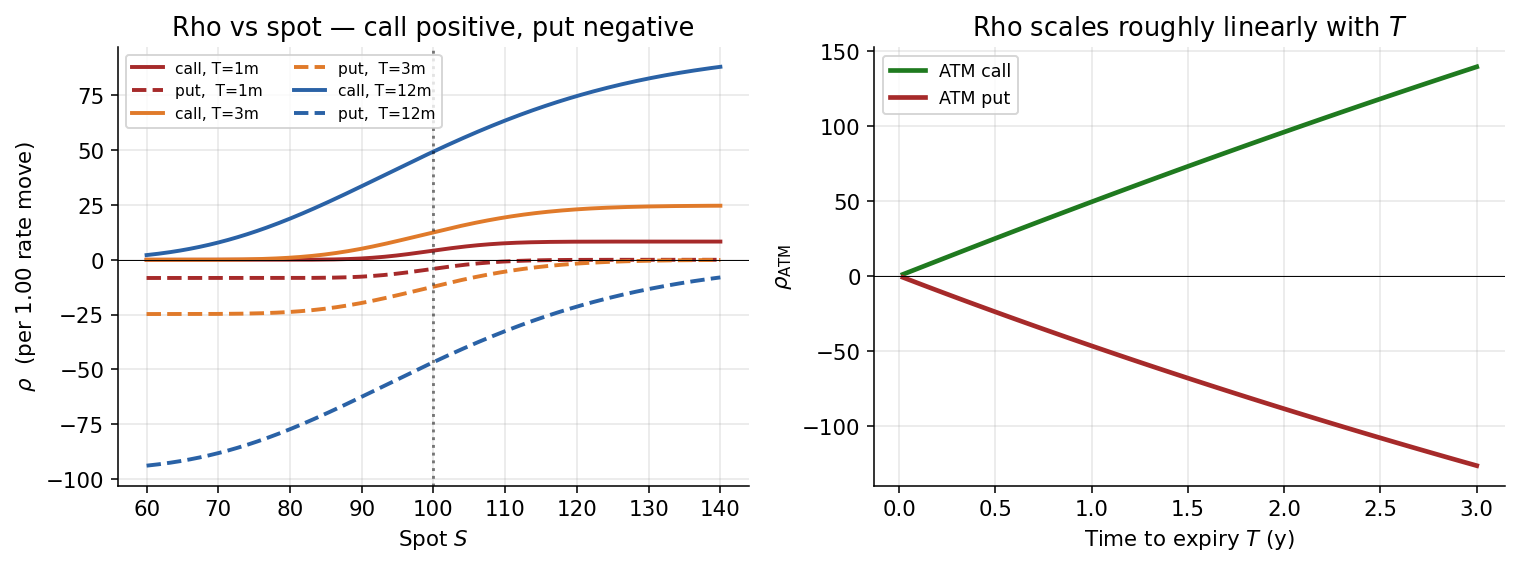
\includegraphics[keepaspectratio]{figures/ch07-rho-call-put.png}}
\caption{Rho vs spot for calls and puts, plus ATM rho vs T}
\end{figure}

\emph{Left: \(\rho\) vs spot for calls (solid) and puts (dashed) at
three maturities. Right: ATM \(\rho\) as a function of \(T\).}

Calls are long rates, puts are short rates, and the magnitude of both
scales roughly linearly in \(T\). For a one-month book, \(\rho\) is
nearly inert; for a one-year book, a \(1\%\) rate shock can move ATM
call value by a third of its premium. Equity-vol traders typically
ignore \(\rho\) until they are warehousing LEAPs or running a
structured-products book --- at which point a separate IR delta desk
picks it up.

\subsection{7.7.3 Vanna --- the cross between spot and
vol}\label{vanna-the-cross-between-spot-and-vol}

\begin{figure}
\centering
\pandocbounded{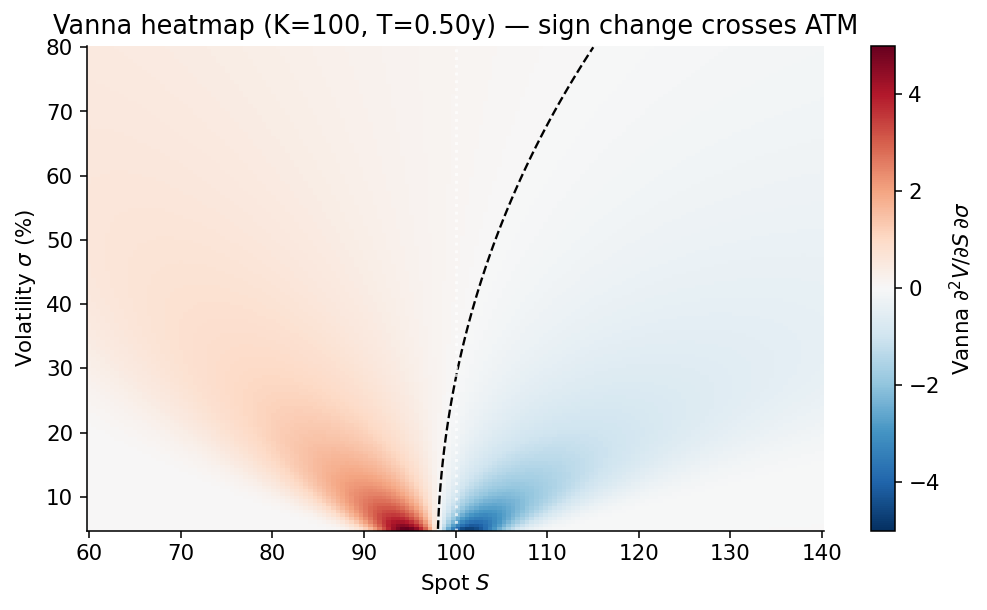
\includegraphics[keepaspectratio]{figures/ch07-vanna.png}}
\caption{Vanna heatmap over (S, sigma) at fixed T, K}
\end{figure}

\emph{Heatmap of \(\partial^2 V / \partial S\,\partial\sigma\) over spot
and implied vol, with the zero contour drawn in dashed black.}

Vanna is the Greek that links spot moves and vol moves: long-vanna
positions earn when spot and vol move together (skew rallies on
sell-offs). The sign change crosses through the strike --- long-call
vanna is \emph{negative} below ATM and \emph{positive} above. Dealers
running exotic books measure vanna because a static vega hedge does not
neutralise it: the first big down-day in the underlying drains delta
into a place where your vega hedge is wrong.

\subsection{7.7.4 Volga --- the smile-curvature
P\&L}\label{volga-the-smile-curvature-pl}

\begin{figure}
\centering
\pandocbounded{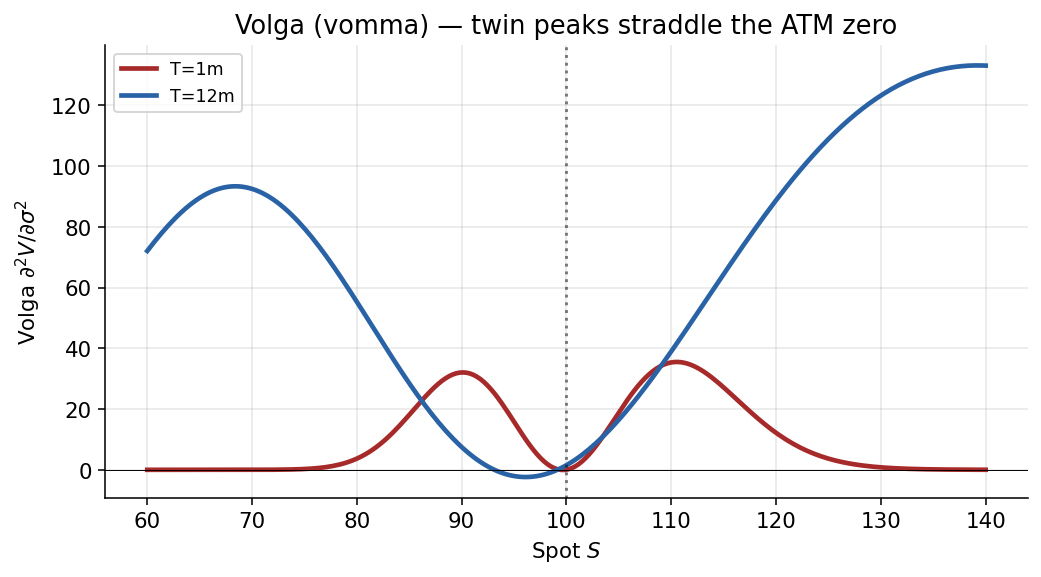
\includegraphics[keepaspectratio]{figures/ch07-volga.png}}
\caption{Volga (vomma) vs spot, two TTMs}
\end{figure}

\emph{\(\partial^2 V/\partial\sigma^2\) for \(T=1\)m and \(T=12\)m.}

Volga has twin peaks straddling the ATM zero --- it is highest in the
\emph{wings}, where vega is small but accelerating in \(\sigma\). A long
strangle is long volga; that is why traders selling tail vol earn when
realised vol of vol is low and lose when the smile lifts at the wings.
The longer-dated curve sits higher and is wider --- vol convexity needs
time to compound.

\subsection{7.7.5 Charm --- delta bleed across the
weekend}\label{charm-delta-bleed-across-the-weekend}

\begin{figure}
\centering
\pandocbounded{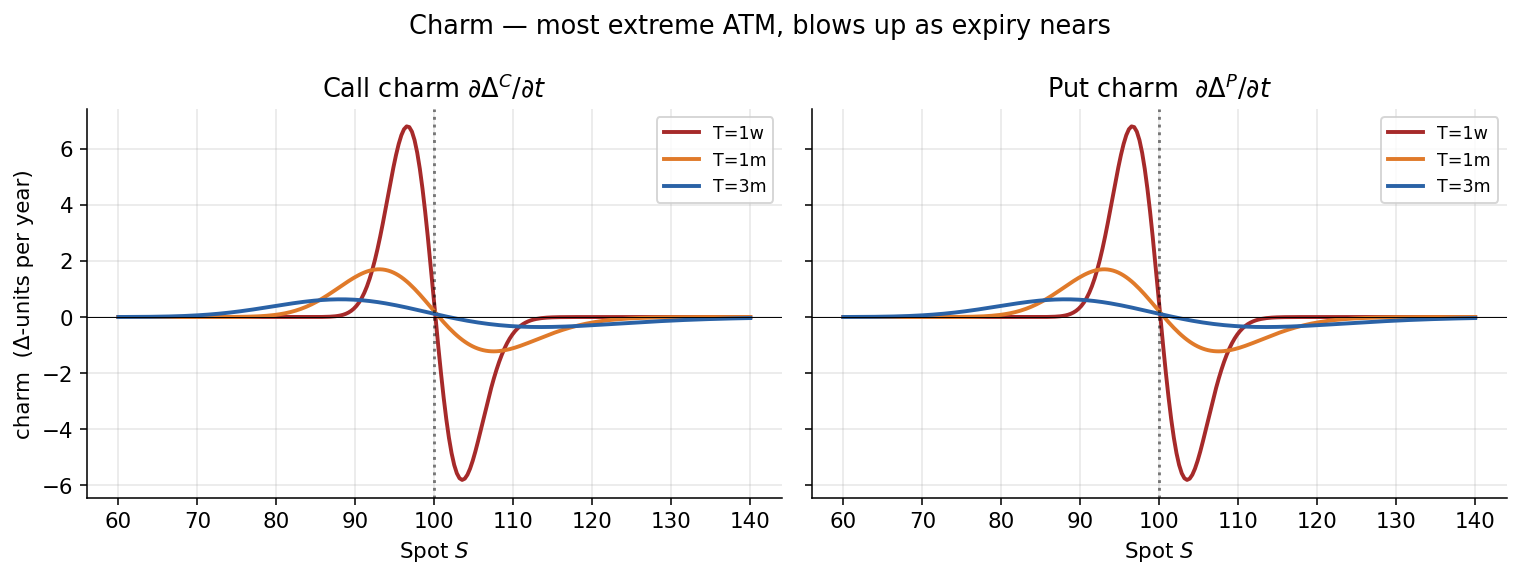
\includegraphics[keepaspectratio]{figures/ch07-charm.png}}
\caption{Charm vs spot for calls and puts, at 1w/1m/3m}
\end{figure}

\emph{Charm \(=\partial\Delta/\partial t\) for calls (left) and puts
(right) at \(T=1\)w, \(1\)m, \(3\)m.}

Charm tells you how much your delta drifts each day even when spot holds
still. The \(1\)-week curve is dramatically more extreme than the
\(3\)-month curve: an OTM option whose delta was \(0.30\) on Friday can
be \(0.15\) on Monday on a flat tape. Market makers quote-stuff their
gamma desk every morning to absorb the weekend charm bleed; this is the
``overnight delta'' that prop traders chase in the open auction.

\subsection{7.7.6 Speed --- gamma's slope}\label{speed-gammas-slope}

\begin{figure}
\centering
\pandocbounded{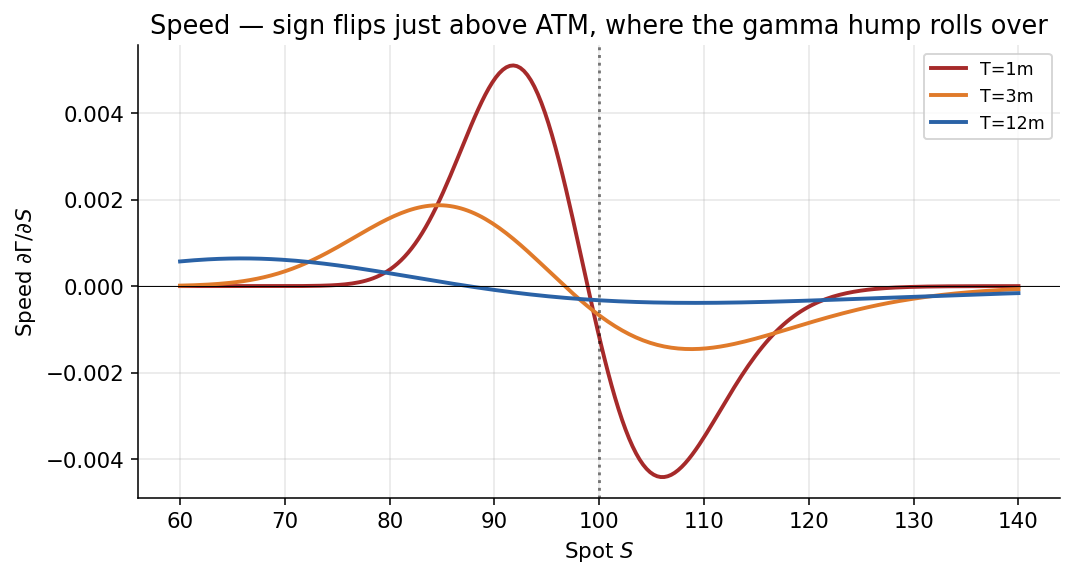
\includegraphics[keepaspectratio]{figures/ch07-speed.png}}
\caption{Speed vs spot, three TTMs}
\end{figure}

\emph{Speed \(=\partial\Gamma/\partial S\) for \(T=1\)m, \(3\)m,
\(12\)m.}

Speed is the third derivative of price w.r.t. spot --- it changes sign
just above the strike, where the gamma hump rolls over. Strategies that
earn from spot-path \emph{cubic} effects (variance-swap convexity
adjustments, butterfly carry) live on speed. For a delta-gamma-hedged
book, residual P\&L from a large spot move is roughly
\(\tfrac{1}{6}\,\text{Speed}\,\Delta S^3\).

\subsection{7.7.7 Color --- gamma's clock}\label{color-gammas-clock}

\begin{figure}
\centering
\pandocbounded{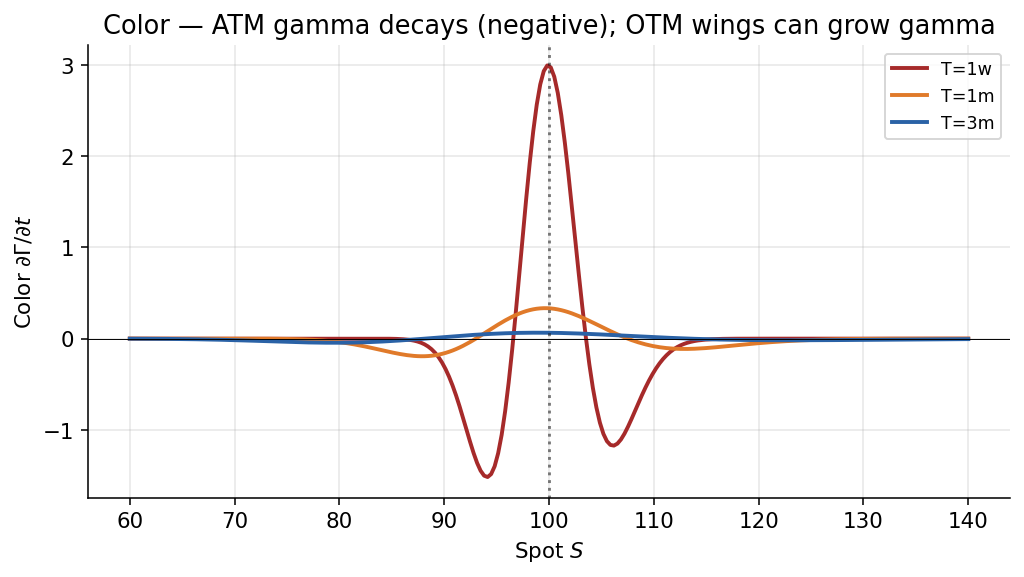
\includegraphics[keepaspectratio]{figures/ch07-color.png}}
\caption{Color vs spot, three TTMs}
\end{figure}

\emph{Color \(=\partial\Gamma/\partial t\) for \(T=1\)w, \(1\)m,
\(3\)m.}

Color says how fast your gamma is changing through time. ATM color is
sharply \emph{negative} --- gamma is the steepest function of \(\tau\)
right at the strike, so an ATM short-gamma desk leaks gamma into the
close. The OTM wings have \emph{positive} color: those strikes build
gamma as expiry approaches, which is why tail-hedgers buy them weeks
ahead, not days.

\subsection{7.7.8 Black-Scholes price
surface}\label{black-scholes-price-surface}

\begin{figure}
\centering
\pandocbounded{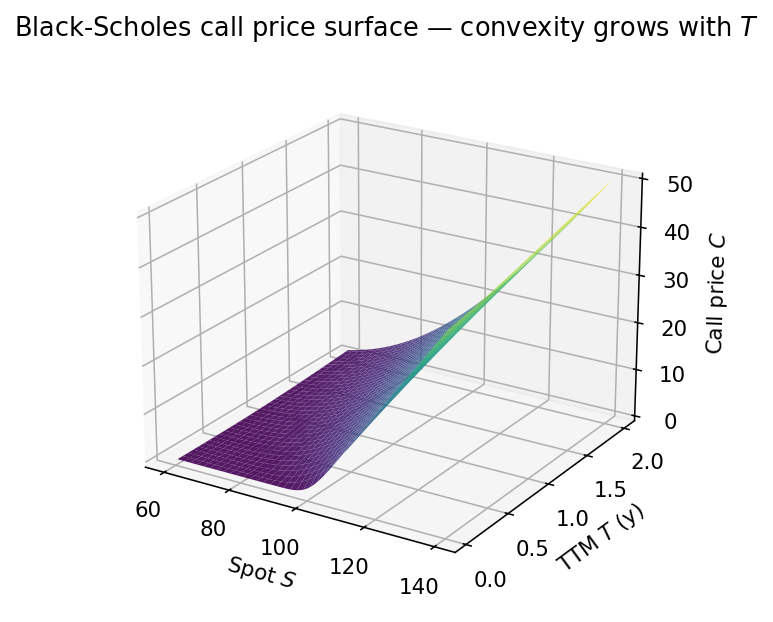
\includegraphics[keepaspectratio]{figures/ch07-bs-price-surface.png}}
\caption{3D BS call price surface over (S, T)}
\end{figure}

\emph{Call value \(C(S, T)\) as a 3D surface; spot in \([60, 140]\), TTM
in \([0.02, 2.0]\).}

The whole chapter so far has been about local first- and second-order
properties of this surface. Stand back and you see the two pieces of
intuition that drive everything: the surface is \emph{increasing and
convex} in spot (positive delta, positive gamma), and \emph{increasing}
in time (positive vega and vega-time product). Convexity emerges visibly
as \(T\) grows --- a long-dated option is much smoother than the kinked
payoff at expiry.

\subsection{7.7.9 Dollar-gamma --- what dealers actually
trade}\label{dollar-gamma-what-dealers-actually-trade}

\begin{figure}
\centering
\pandocbounded{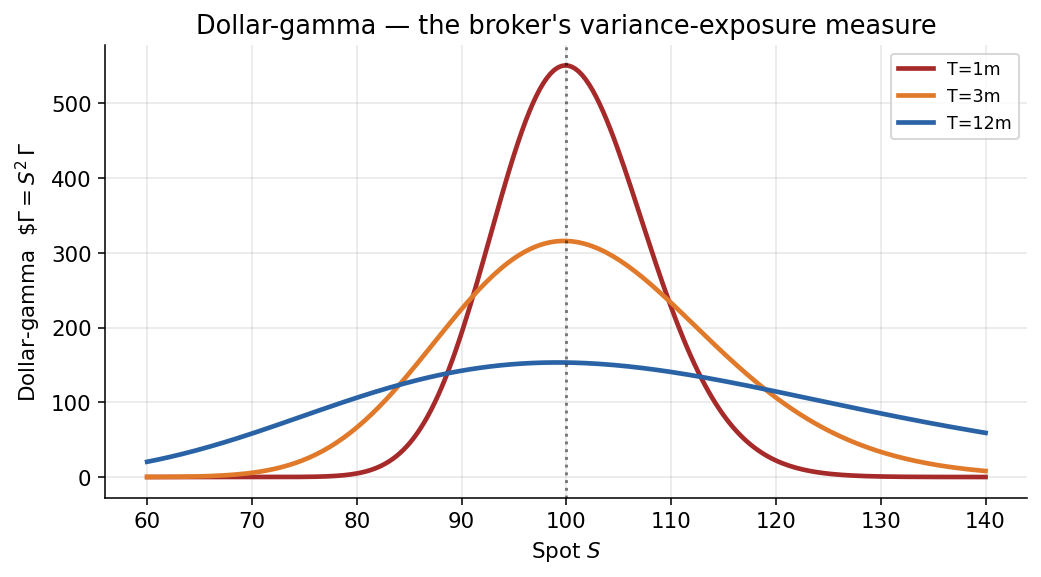
\includegraphics[keepaspectratio]{figures/ch07-dollar-gamma-vs-spot.png}}
\caption{Dollar-gamma vs spot, three TTMs}
\end{figure}

\emph{\(\$\Gamma = S^2\,\Gamma\) vs spot at three maturities.}

Vanilla gamma is in (option-units / share\(^2\)) and depends on the
underlying's price level. Dealers normalise by \(S^2\) to get
\emph{dollar-gamma} --- the P\&L impact of a \(1\%\) spot move squared.
The peak shifts very slightly above the strike (because \(S^2\) grows
faster than \(\Gamma\) falls on the right wing), and it is the flatter,
broader profile that variance-swap and dispersion desks quote against.

\subsection{7.7.10 The strike ladder --- Greeks for an ATM expiry-1m
book}\label{the-strike-ladder-greeks-for-an-atm-expiry-1m-book}

\begin{figure}
\centering
\pandocbounded{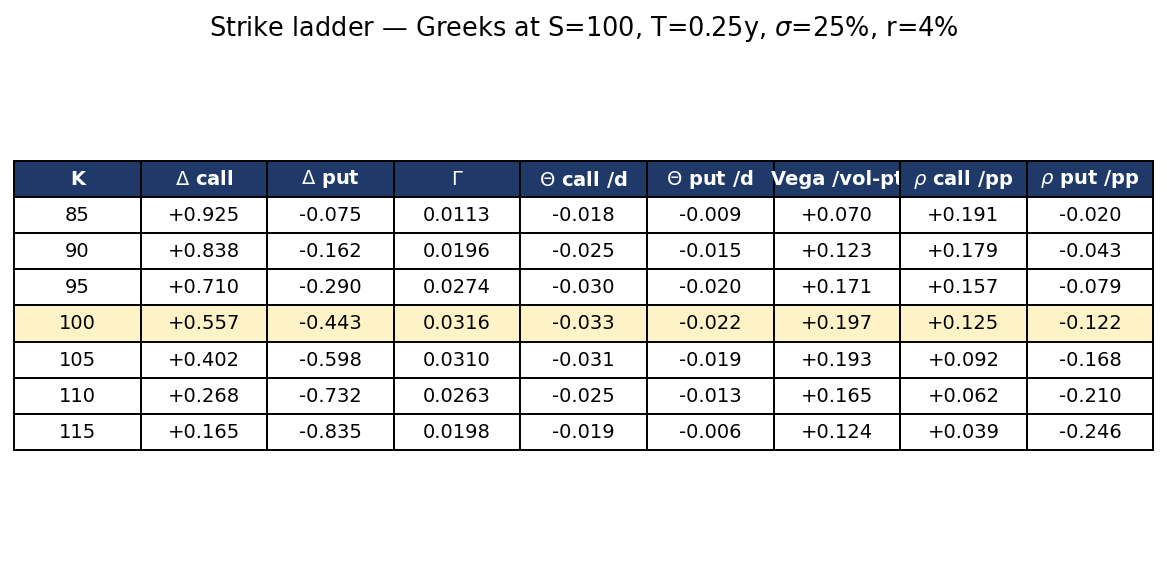
\includegraphics[keepaspectratio]{figures/ch07-greek-table-strike-ladder.png}}
\caption{Strike-ladder table of all Greeks}
\end{figure}

\emph{All major Greeks for calls and puts on a \(T=0.25\)y,
\(\sigma=25\%\) book; ATM row highlighted.}

A working trader's screen looks like this table. Note the parity
identities check by inspection: every row has \(\Delta^C - \Delta^P
= 1\) (since \(q=0\), \(e^{-q\tau}=1\)) and \(\Gamma\) identical for
call and put. Theta and rho do \emph{not} match across call/put ---
those gaps are exactly (7.77) and (7.78). The ATM row carries the
largest \(\Gamma\), the largest \(|\Theta|\), and the largest vega ---
three reasons it is also the most expensive line on the screen.

\subsection{7.7.11 Pin risk --- the digital-delta
blow-up}\label{pin-risk-the-digital-delta-blow-up}

\begin{figure}
\centering
\pandocbounded{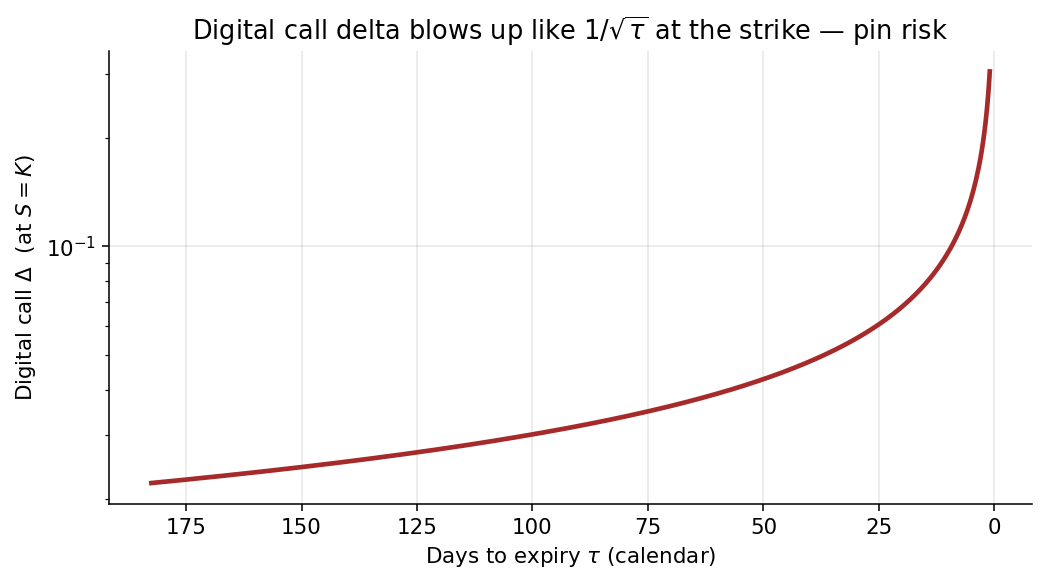
\includegraphics[keepaspectratio]{figures/ch07-pin-risk-digital-delta.png}}
\caption{Digital call delta vs days to expiry at S=K}
\end{figure}

\emph{Delta of a digital call struck at the spot, plotted (log-y) vs
calendar days to expiry.}

A vanilla option's gamma blows up as \(1/\sqrt{\tau}\) at the strike; a
\emph{digital} option's delta does. With days running out (x-axis
inverted, expiry on the right), the digital delta --- which equals the
\(\$1\) size of the payoff times the gamma kernel --- explodes by more
than two orders of magnitude in the last week. This is why short-dated
structured-product issuers (autocallables, dual-currency deposits) cap
exposure to single strikes: pin risk in the last hour is uninsurable in
size.

\subsection{7.7.12 Vega across the smile}\label{vega-across-the-smile}

\begin{figure}
\centering
\pandocbounded{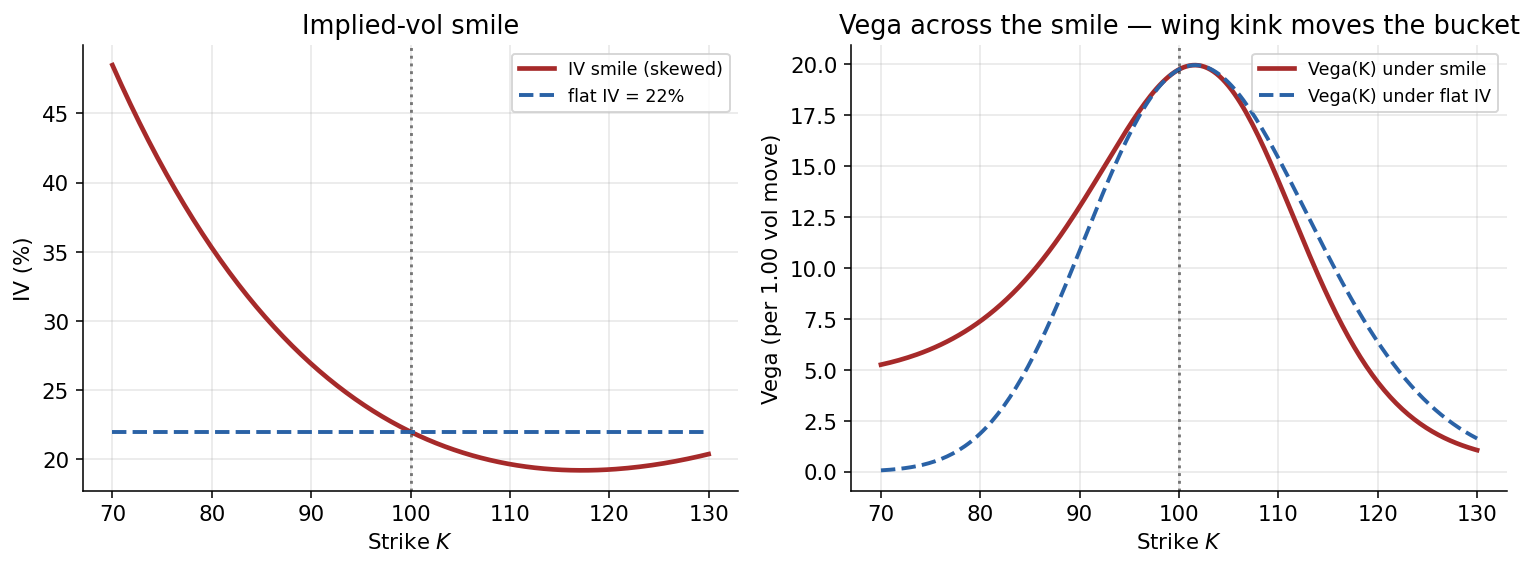
\includegraphics[keepaspectratio]{figures/ch07-skew-vs-vega.png}}
\caption{IV smile and vega(K) under smile vs flat IV}
\end{figure}

\emph{Left: a parameterised IV smile \(\sigma(K)=\sigma_{\rm atm} + a
\log(K/S) + b\log^2(K/S)\) with \(a=-0.35\), \(b=1.10\). Right: vega per
strike under that smile vs under a flat \(22\%\) IV.}

Vega's bell-shape gets \emph{bent} by the smile: down-side strikes (with
elevated IV) carry more vega than the flat-IV baseline would suggest,
and the OTM call wing gets reweighted up by the convex smile too. Dealer
vega exposure does not concentrate where vega itself is largest in the
flat world --- it concentrates wherever the smile is steepest. This is
why ``vega bucketing by strike'' has replaced ``vega bucketing by ATM
only'' everywhere a real skew exists.

\subsection{7.7.13 Gamma scalping --- the variance-risk-premium
picture}\label{gamma-scalping-the-variance-risk-premium-picture}

\begin{figure}
\centering
\pandocbounded{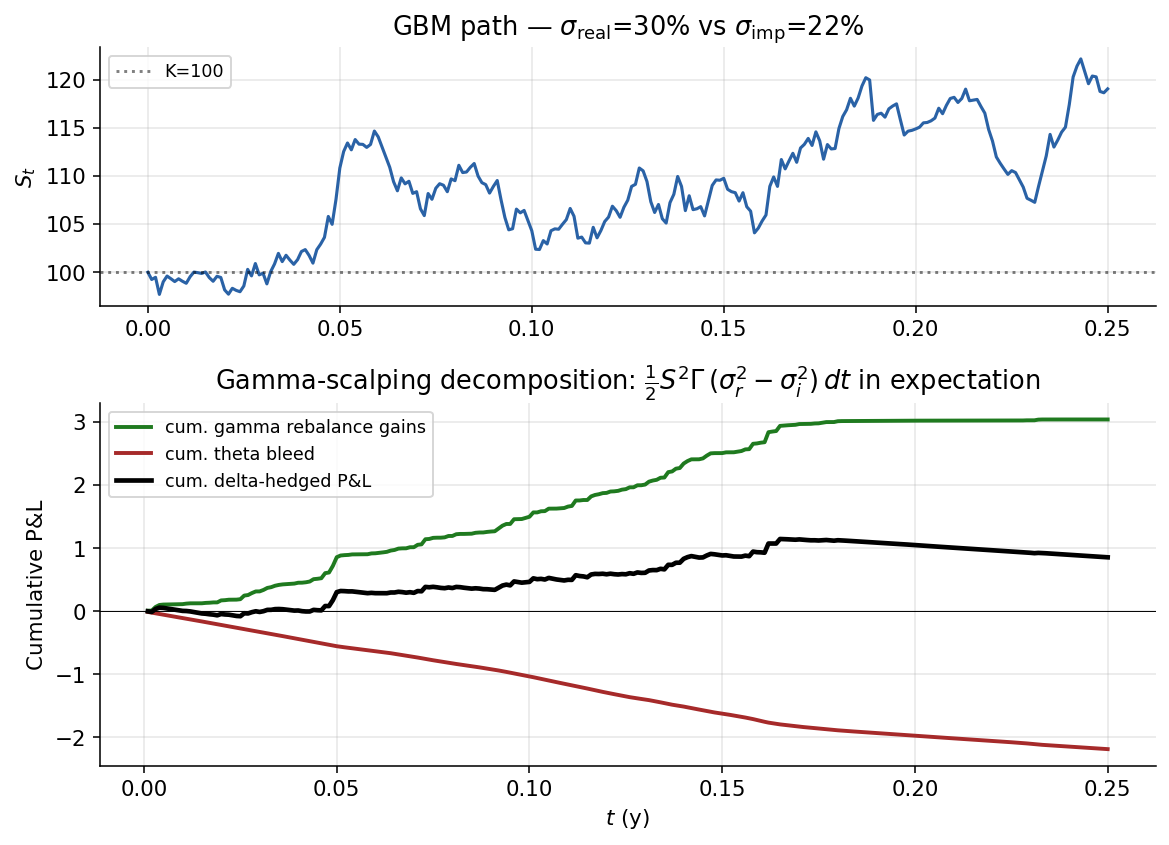
\includegraphics[keepaspectratio]{figures/ch07-gamma-scalping-pnl.png}}
\caption{Cumulative gamma scalping vs theta bleed on a GBM path}
\end{figure}

\emph{Top: a Monte Carlo GBM path with \(\sigma_{\rm real}=30\%\),
hedged at \(\sigma_{\rm imp}=22\%\). Bottom: cumulative theta bleed
(red), cumulative gamma rebalance gains (green), and net delta-hedged
P\&L (black).}

This picture is the visual identity behind Section 7.2.8's
variance-risk-premium claim. The dealer is short theta every day at a
rate set by \emph{implied} vol; they earn back \(\tfrac12 S^2\Gamma\,
(\Delta S)^2\) at each rebalance, whose expected value scales with
\emph{realised} vol squared. When
\(\sigma_{\rm real}>\sigma_{\rm imp}\), green outpaces red and the
hedged book earns the difference. When the inequality flips, the hedger
pays for vol they never used. One sample path looks noisy; ten thousand
average to the closed-form
\(\tfrac12\int_0^T S_t^2 \Gamma_t (\sigma_{\rm real}^2 - \sigma_{\rm
imp}^2)\,dt\).

\begin{center}\rule{0.5\linewidth}{0.5pt}\end{center}

\section{7.8 Key Takeaways}\label{key-takeaways-6}

\begin{enumerate}
\def\labelenumi{\arabic{enumi}.}
\item
  \textbf{Delta-gamma hedging neutralises two derivatives.} Holding
  \(-\Delta^g\) shares of stock and \(-\gamma\) units of an auxiliary
  option \(h\), with \(\gamma = \Gamma^g / \Gamma^h\), eliminates both
  the first-order and second-order Taylor terms of the hedged P\&L. The
  residual is cubic in \(\Delta S\) instead of quadratic, and its
  standard deviation under \(N\)-grid rebalancing scales as \(1/N\)
  rather than \(1/\sqrt{N}\).
\item
  \textbf{Vega is the volatility-input sensitivity, not a tradable
  Greek.} \(\mathcal{V} = S\,\sqrt{T-t}\,\Phi'(d_+)\) peaks ATM and
  decays as \(\sqrt{T-t}\to 0\). Vega-hedging requires a \emph{second
  option} with linearly independent gamma-vega profile (system 7.36),
  because volatility itself is not a tradable asset under
  constant-\(\sigma\) Black-Scholes.
\item
  \textbf{Continuous-dividend BSM PDE differs only in the drift
  coefficient.}
  \(\partial_t g + (r-q)\,S\,\partial_S g + \tfrac12\sigma^2 S^2\partial_{SS} g = r\,g\).
  The discount rate on the RHS is still \(r\) (the option pays nothing
  in the interim), but the risk-neutral drift of \(S\) is reduced by
  \(q\).
\item
  \textbf{Forward reformulation collapses the dividend correction.}
  Defining \(F_t = S_t e^{(r-q)(T-t)}\), the dividend yield disappears
  into the forward price; the option becomes Black-76 with no drift.
\item
  \textbf{Put-call parity drives the cross-Greek identities.} From
  \(C - P = S e^{-q\tau} - K e^{-r\tau}\) we read off
  \(\Delta^C - \Delta^P = e^{-q\tau}\), \(\Gamma^C = \Gamma^P\),
  \(\mathcal V^C = \mathcal V^P\), and the asymmetric theta/rho gaps.
  These identities are \emph{model-free}: they hold in every
  arbitrage-free model in which parity is imposed.
\item
  \textbf{Pin risk is the \(1/\sqrt{\tau}\) blow-up of ATM gamma.} As
  \(\tau\downarrow 0\),
  \(\Gamma_{\text{ATM}} \sim 1/(K\sigma\sqrt{2\pi\tau})\), so a short
  ATM option on expiry day has a delta that whips between \(0\) and
  \(\pm e^{-q\tau}\) on tiny spot moves. Market makers flatten ATM
  exposure into the close.
\item
  \textbf{Self-financing is a covariation condition, not a slogan.} The
  clean \(\mathrm dV = \alpha\,\mathrm dS + \beta\,\mathrm dM\) requires
  \(\mathrm d\alpha_t\,S_t + \mathrm d[\alpha, S]_t +
  \mathrm d\beta_t\,M_t + \mathrm d[\beta, M]_t = 0\). The covariation
  term \(\mathrm d[\alpha, S] = \Gamma\,\sigma^2 S^2\,\mathrm dt\) is
  what produces the \(\tfrac12\sigma^2 S^2\partial_{SS}\) piece of the
  BS PDE in the first place.
\item
  \textbf{Transaction costs price as a volatility premium.} Leland's
  adjustment
  \(\sigma^2_{\text{Leland}} = \sigma^2 + c\sigma\sqrt{8/(\pi\Delta t)}\)
  raises the dealer's effective vol by the spread \(c\) and rebalance
  frequency. At \(c=1\) bp, daily rebalancing adds \(\approx 0.6\) vol
  points; at \(c=10\) bp (stressed), the addition jumps to \(\approx 6\)
  points. Real prices are BS plus Leland plus XVA plus skew plus
  liquidity premia.
\end{enumerate}

\begin{center}\rule{0.5\linewidth}{0.5pt}\end{center}

\section{7.9 Reference Formulas
Appendix}\label{reference-formulas-appendix-1}

{\def\LTcaptype{none} % do not increment counter
\begin{longtable}[]{@{}
  >{\raggedright\arraybackslash}p{(\linewidth - 2\tabcolsep) * \real{0.5000}}
  >{\raggedright\arraybackslash}p{(\linewidth - 2\tabcolsep) * \real{0.5000}}@{}}
\toprule\noalign{}
\begin{minipage}[b]{\linewidth}\raggedright
Label
\end{minipage} & \begin{minipage}[b]{\linewidth}\raggedright
Formula
\end{minipage} \\
\midrule\noalign{}
\endhead
\bottomrule\noalign{}
\endlastfoot
(7.3) & \(\Gamma = \Phi'(d_+)/(S\,\sigma\sqrt{T-t})\),
\(\mathcal V = S\sqrt{T-t}\,\Phi'(d_+)\) \\
(7.11) & \(\gamma_t = \Gamma^g/\Gamma^h\),
\(\alpha_t = \Delta^g - \gamma_t\,\Delta^h\) (delta-gamma hedge
weights) \\
(7.29) & \(\mathrm{Var}_{\text{delta-only}} \sim \sigma^4 T^2 / N\)
(gamma-residual scaling) \\
(7.30) & \(\mathrm{Var}_{\text{delta-gamma}} \sim \sigma^6 T^3 / N^2\)
(cubic-residual scaling) \\
(7.33) & \(\mathcal V_t = S_t\,\sqrt{T-t}\,\Phi'(d_+)\) (vanilla
vega) \\
(7.36) &
\(\big(1,\Delta^{h_1},\Delta^{h_2};0,\Gamma^{h_1},\Gamma^{h_2};0,\mathcal V^{h_1},\mathcal V^{h_2}\big)(\alpha_t,\gamma^1_t,\gamma^2_t)^\top = (\Delta^g,\Gamma^g,\mathcal V^g)^\top\)
(delta-gamma-vega match) \\
(7.49) &
\(\partial_t g + (r-q)\,S\,\partial_S g + \tfrac12\sigma^2 S^2\partial_{SS} g = r\,g\)
(BSM PDE with continuous yield) \\
(7.51) & \(g(t,S) = S\,e^{-q\tau}\Phi(d_+) - K\,e^{-r\tau}\Phi(d_-)\)
(BSM call with dividends) \\
(7.52) &
\(d_\pm = [\ln(S/K) + (r - q \pm \tfrac12\sigma^2)\tau]/(\sigma\sqrt\tau)\) \\
(7.55) & Black-76 form via \(F_t = S_t e^{(r-q)(T-t)}\) --- dividend
absorbed into forward \\
(7.57) & \(\Gamma_t = e^{-q\tau}\Phi'(d_+)/(S\sigma\sqrt\tau)\)
(dividend-adjusted gamma) \\
(7.58) & \(\mathcal V_t = S\,e^{-q\tau}\sqrt\tau\,\Phi'(d_+)\)
(dividend-adjusted vega) \\
(7.66) &
\(\mathrm d\alpha_t S_t + \mathrm d[\alpha,S]_t + \mathrm d\beta_t M_t + \mathrm d[\beta,M]_t = 0\)
(self-financing in covariation form) \\
(7.67) & \(\mathrm d[\alpha, S]_t = \Gamma\,\sigma^2 S^2\,\mathrm dt\)
(delta-hedge covariation) \\
(7.68) & Self-financing with proportional costs: RHS becomes
\(-c\,|\mathrm d\alpha_t|S_t - c\,|\mathrm d\gamma_t|h_t\) \\
(7.69) &
\(\sigma^2_{\text{Leland}} = \sigma^2 + c\,\sigma\,\sqrt{8/(\pi\Delta t)}\)
(Leland volatility adjustment) \\
(7.70) & \(C(t,S) - P(t,S) = S\,e^{-q\tau} - K\,e^{-r\tau}\) (put-call
parity) \\
(7.73) & \(\Delta^C - \Delta^P = e^{-q\tau}\) (parity-delta) \\
(7.75) &
\(\Gamma^C = \Gamma^P = e^{-q\tau}\Phi'(d_+)/(S\sigma\sqrt\tau)\)
(parity-gamma) \\
(7.76) & \(\mathcal V^C = \mathcal V^P\) (parity-vega) \\
(7.77) & \(\Theta^C - \Theta^P = -q\,S\,e^{-q\tau} + r\,K\,e^{-r\tau}\)
(parity-theta) \\
(7.78) & \(\rho^C - \rho^P = \tau\,K\,e^{-r\tau}\) (parity-rho) \\
(7.79) & Synthetic forward: \(C - P = S\,e^{-q\tau} - K\,e^{-r\tau}\)
replicates a long forward + short bond \\
\end{longtable}
}

\begin{center}\rule{0.5\linewidth}{0.5pt}\end{center}

\section{\texorpdfstring{Appendix A --- Empirical Proof of the
\(\sqrt{30/\tau}\) Vol-Shock
Scaling}{Appendix A --- Empirical Proof of the \textbackslash sqrt\{30/\textbackslash tau\} Vol-Shock Scaling}}\label{appendix-a-empirical-proof-of-the-sqrt30tau-vol-shock-scaling}

The vega-hedging machinery of §7.3 treats \(\sigma\) as a single number
and computes \(\mathcal V = \partial_\sigma g\) under the constant-vol
Black-Scholes assumption. In practice a desk holds positions across a
maturity spectrum from weekly options to LEAPS, every maturity has its
own implied vol, and ``what happens if vol shocks one point'' has no
unique answer. The natural-language phrase masks a modelling choice:
does \emph{the entire surface} move one point in parallel, or does only
the front of the curve move one point and the back move less? The two
stress tests differ by enough on a real vega book that the choice of
convention is itself a risk-management decision.

The workhorse heuristic is to scale shocks by \(\sqrt{30/\tau}\), where
\(\tau\) is days to expiry: a 1-point shock to 30-day vol is accompanied
by a \(\sqrt{30/90}\approx 0.577\) point shock to 90-day vol and a
\(\sqrt{30/180}\approx 0.408\) point shock to 6-month vol.~This appendix
tests it against the CBOE VIX-term-structure indices. The headline
result is that the \(\sqrt{}\)-rule is roughly correct but the empirical
exponent is shallower than \(0.5\): the back of the curve moves
\emph{more} than the heuristic claims when the front shocks.

\subsection{A.1 The practitioner
setup}\label{a.1-the-practitioner-setup}

Define the \emph{term beta}

\[
\beta(\tau) \;\equiv\; \frac{\mathbb E\big[\Delta\sigma_{\tau} \mid \Delta\sigma_{30}\big]}{\Delta\sigma_{30}}, \tag{7.A1}
\]

the expected one-day change in the \(\tau\)-day implied vol per unit
one-day change in 30-day vol.~Under a parallel-surface shock
\(\beta(\tau)\equiv 1\) for every \(\tau\). Under a front-localised
shock \(\beta(\tau)\to 0\) for large \(\tau\). Between those two
extremes lives every realistic stress test, and the \(\sqrt{30/\tau}\)
heuristic is one particular interpolant.

The choice of \(\beta(\tau)\) matters because the vega of an option
scales as \(\sqrt{\tau}\) (see (7.33)). A book with \(\$1\)mm vega at 30
days, \(\$2\)mm at 90 days, and \(\$4\)mm at 180 days takes a \(-\$7\)mm
hit under a parallel 1-vol shock. Under the \(\sqrt{}\)-rule the same
shock costs \(1\cdot 1 + 2\cdot 0.577 + 4\cdot 0.408 \approx \$3.78\)mm
--- less than half. A trader who quotes the same number for the two
stress tests is not making a small error; they are confusing the shape
of their book by close to a factor of two. The point of this appendix is
to argue, with data, that the second number is the correct one.

\subsection{A.2 Theoretical
motivation}\label{a.2-theoretical-motivation}

Why \(1/\sqrt{\tau}\)? Take a Heston-style CIR variance \(\mathrm dv_t =
\kappa(\theta - v_t)\mathrm dt + \xi\sqrt{v_t}\,\mathrm dW^v_t\). The
conditional expectation of the time-averaged variance over
\([t, t+\tau]\) given the instantaneous state \(v_t\) has analytic
sensitivity

\[
\frac{\partial}{\partial v_t}\,\mathbb E_t\!\left[\frac{1}{\tau}\int_t^{t+\tau}\!v_s\,\mathrm ds\right] \;=\;
\frac{1 - e^{-\kappa\tau}}{\kappa\tau}. \tag{7.A3}
\]

For \(\kappa\tau\in[0.2, 2]\) --- the practitioner range under typical
SPX mean-reversion \(\kappa\approx 2\)--4 yr\(^{-1}\) --- this
expression is well-approximated by \((\kappa\tau)^{-1/2}\) up to a
constant prefactor, the \(1/\sqrt{\tau}\) that the heuristic encodes. An
analogous derivation under log-OU vol gives the same scaling. Outside
that range the rule breaks down: for \(\tau\to 0\) the response
saturates at 1, and for \(\tau\to\infty\) it decays as \(1/\tau\). The
heuristic is calibrated to the middle range, and we test it on exactly
that range.

\subsection{A.3 Data}\label{a.3-data}

The CBOE publishes four term-structure indices that are tailor-made for
this question: VIX9D (9-day), VIX (30-day), VIX3M (90-day), and VIX6M
(180-day). Each is the model-free implied-volatility strip integral of
SPX options at the corresponding tenor, rolled daily to maintain
constant days-to-expiry. We pull the four series from Yahoo Finance
under tickers \texttt{\^{}VIX9D}, \texttt{\^{}VIX}, \texttt{\^{}VIX3M},
\texttt{\^{}VIX6M}, inner-join on dates, and take daily differences. The
joined sample runs 2011-01-03 through 2026-05-15 for \(n = 3{,}864\)
daily observations. The start date is constrained by the publication
history of VIX3M and VIX6M, neither of which extends back to the Lehman
crisis.

One caveat: the VIX indices are \emph{model-free} IV --- weighted strip
integrals of SPX option prices, not Black-Scholes ATM IV. The
distinction matters for absolute-level questions but for term-structure
regression the bias affects every tenor symmetrically and the
\(\beta(\tau)\) ratios are unaffected to first order.

\subsection{A.4 Per-tenor regression}\label{a.4-per-tenor-regression}

For each tenor \(\tau\in\{9, 30, 90, 180\}\) we run a no-intercept OLS
of \(\Delta\sigma_\tau\) on \(\Delta\sigma_{30}\):

\[
\Delta\sigma_\tau^{(t)} \;=\; \beta(\tau)\,\Delta\sigma_{30}^{(t)} \;+\; \varepsilon_t. \tag{7.A4}
\]

The intercept is suppressed because under any homogeneous shock the
zero-shock response must be zero --- including a constant absorbs
non-shock-driven drift that we have no reason to attribute to \(\beta\).
The results, with heteroskedasticity-consistent standard errors, are

{\def\LTcaptype{none} % do not increment counter
\begin{longtable}[]{@{}rrrr@{}}
\toprule\noalign{}
\(\tau\) & \(\beta(\tau)\) & SE & \(R^2\) \\
\midrule\noalign{}
\endhead
\bottomrule\noalign{}
\endlastfoot
9 d & \(1.5170\) & \(\pm 0.0077\) & \(0.9090\) \\
30 d & \(1.0000\) & (by construction) & \(1.0000\) \\
90 d & \(0.6413\) & \(\pm 0.0029\) & \(0.9284\) \\
180 d & \(0.4589\) & \(\pm 0.0029\) & \(0.8677\) \\
\end{longtable}
}

The standard errors are tight at every tenor --- with 3,864 days of data
the \(\beta\)s are pinned to within a tenth of a vol point per vol
point. The \(R^2\) values decay monotonically with \(\tau\), which is
the expected signature of a noisier signal at the back of the curve: a
one-point move in 30-day vol explains 93\% of the contemporaneous
variance of 90-day vol but only 87\% of 180-day vol, the residual being
term-structure-localised shocks (curve-twist events) that move one tenor
without moving the other.

\begin{figure}
\centering
\pandocbounded{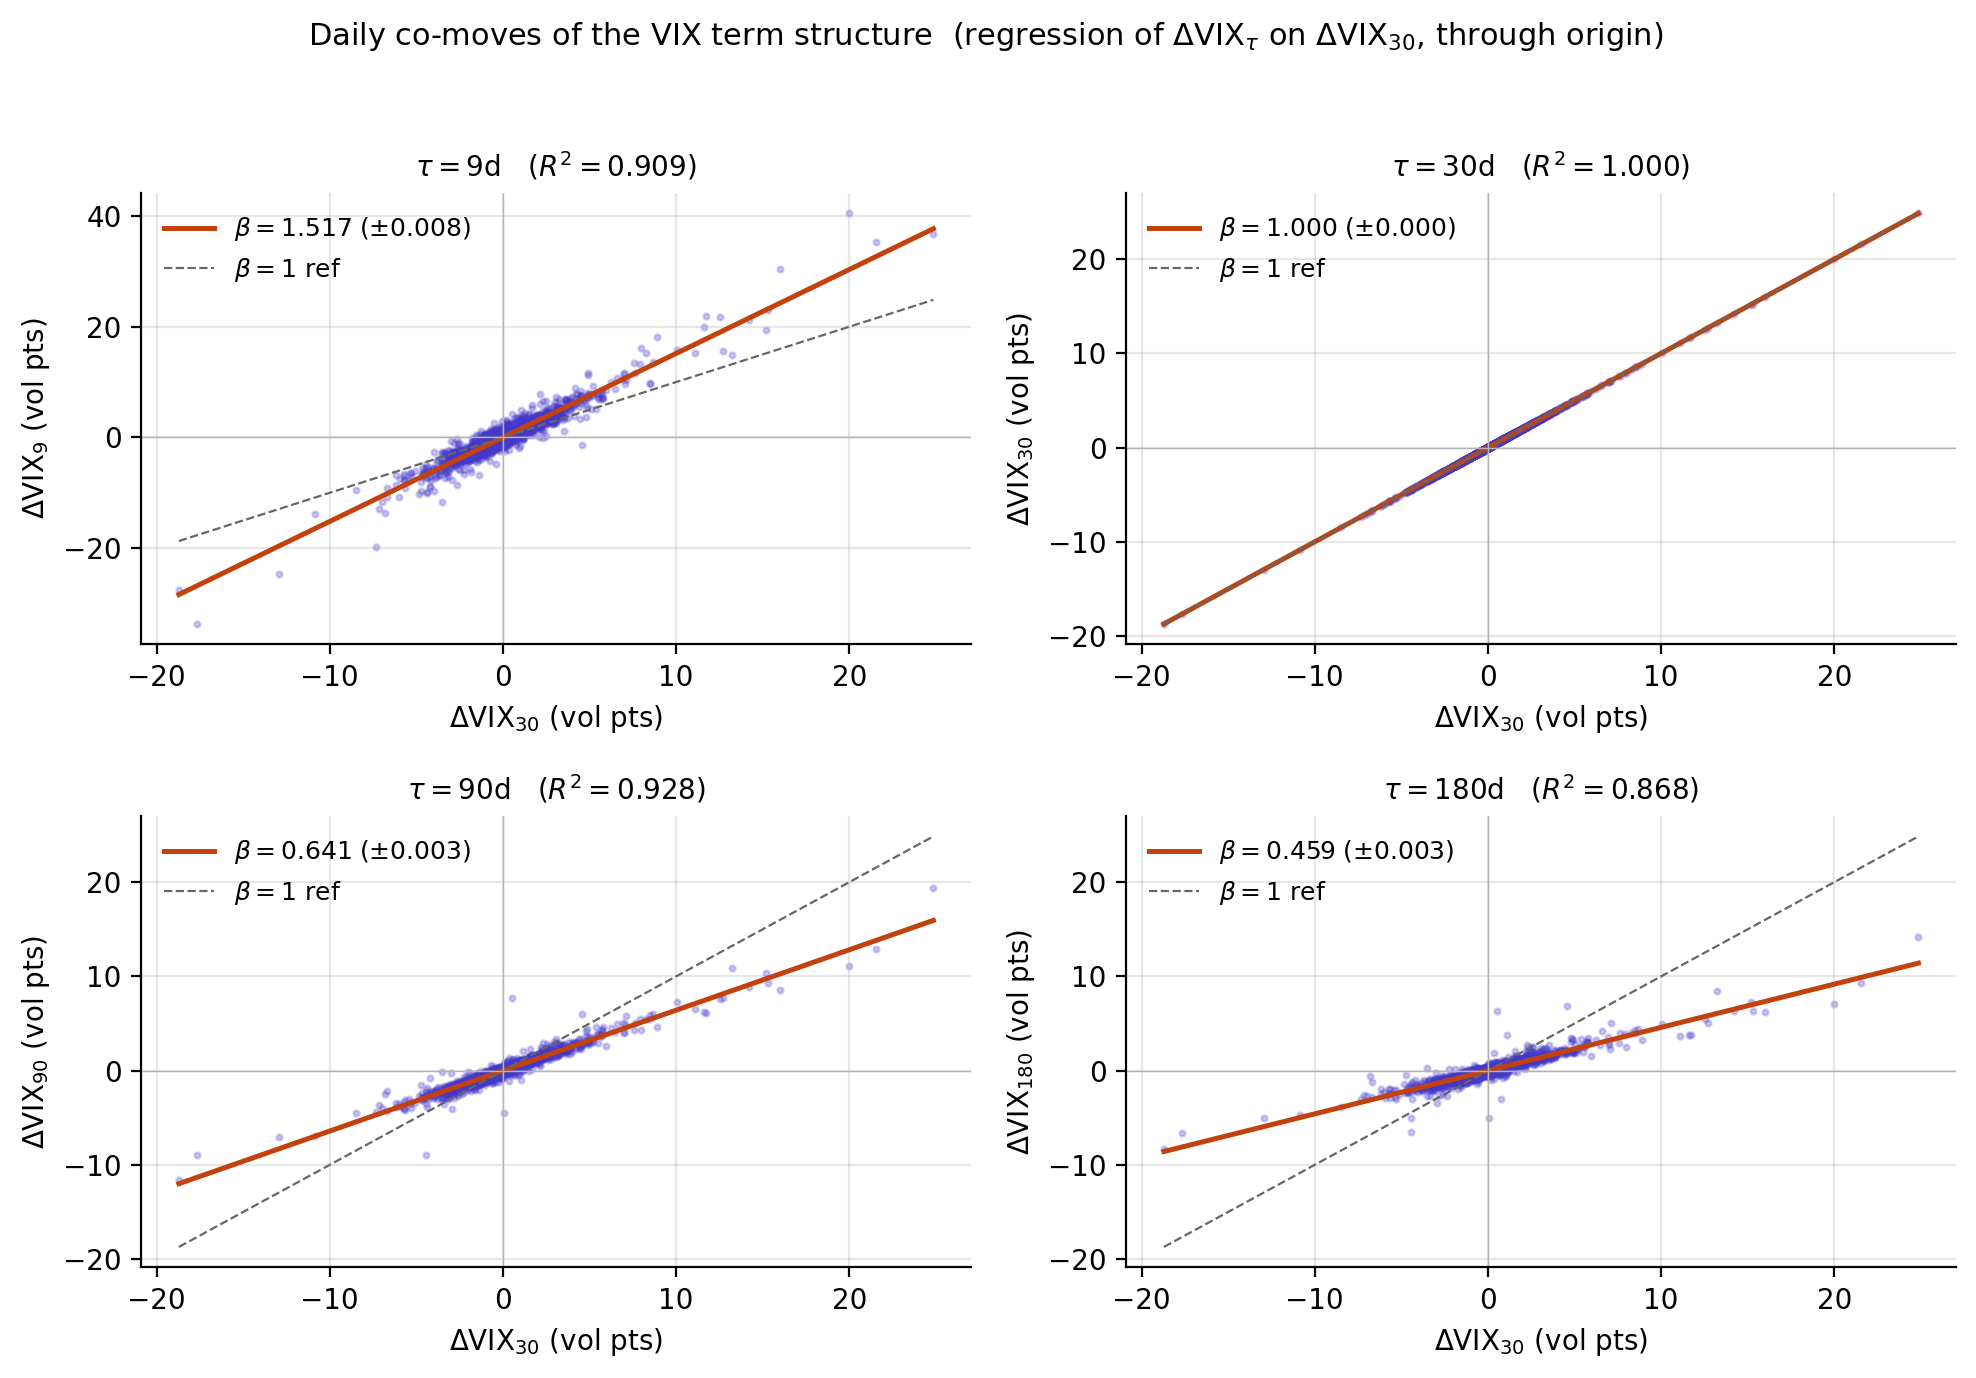
\includegraphics[keepaspectratio]{figures/ch7-vol-shock-scaling-fit.png}}
\caption{Per-tenor regression of \(\Delta\sigma_\tau\) on
\(\Delta\sigma_{30}\) for the four CBOE term-structure indices}
\end{figure}

\emph{Four-panel scatter of daily \(\Delta\sigma_\tau\) against
\(\Delta\sigma_{30}\) for \(\tau\in\{9, 30, 90, 180\}\) days, with the
no-intercept OLS regression line and its slope \(\beta(\tau)\)
annotated. The 30-day panel is the identity by construction. The 9-day
panel has the steepest slope and the fattest tails --- front vol is both
more responsive and more idiosyncratic. The 180-day panel has the
shallowest slope and the most clustered cloud: the back of the curve is
anchored.}

The four-point picture is qualitatively what the heuristic predicts:
front vol is more responsive than 30-day vol; the back of the curve is
less responsive. The 9-day \(\beta = 1.517\) should be compared with the
heuristic's prediction \(\sqrt{30/9}=1.826\) --- the heuristic
\emph{overshoots} front vol, by about \(20\%\). The 90-day
\(\beta = 0.641\) should be compared with the heuristic's
\(\sqrt{30/90}=0.577\) --- the heuristic \emph{undershoots} by about
\(11\%\). The 180-day \(\beta = 0.459\) should be compared with the
heuristic's \(\sqrt{30/180}=0.408\) --- the heuristic undershoots by
\(12\%\). Both errors are in the same direction at the back: long-dated
vols move more than the \(\sqrt{}\)-rule predicts.

\subsection{A.5 Power-law fit}\label{a.5-power-law-fit}

To formalise that observation, fit a power law
\(\beta(\tau) = (30/\tau)^\alpha\) across the four points by log-linear
regression on \(\log\beta(\tau)\) versus \(\log(\tau/30)\):

\[
\log\beta(\tau) \;=\; -\alpha\,\log(\tau/30) \;+\; \varepsilon. \tag{7.A5}
\]

The fit gives

\[
\hat\alpha \;=\; 0.4066, \qquad \text{SE} \;=\; \pm 0.0259, \qquad R^2 \;=\; 0.9897. \tag{7.A6}
\]

The empirical exponent is \(0.41\), not \(0.50\). The standard error is
small enough --- three units in the third decimal --- that
\(\alpha = 0.5\) is rejected with high confidence on this sample. The
\(R^2\) is \(0.99\), so a single-exponent power law is a sufficient
description of the term-beta curve at the resolution of the four CBOE
tenors; we are not underfitting some richer functional form.

\begin{figure}
\centering
\pandocbounded{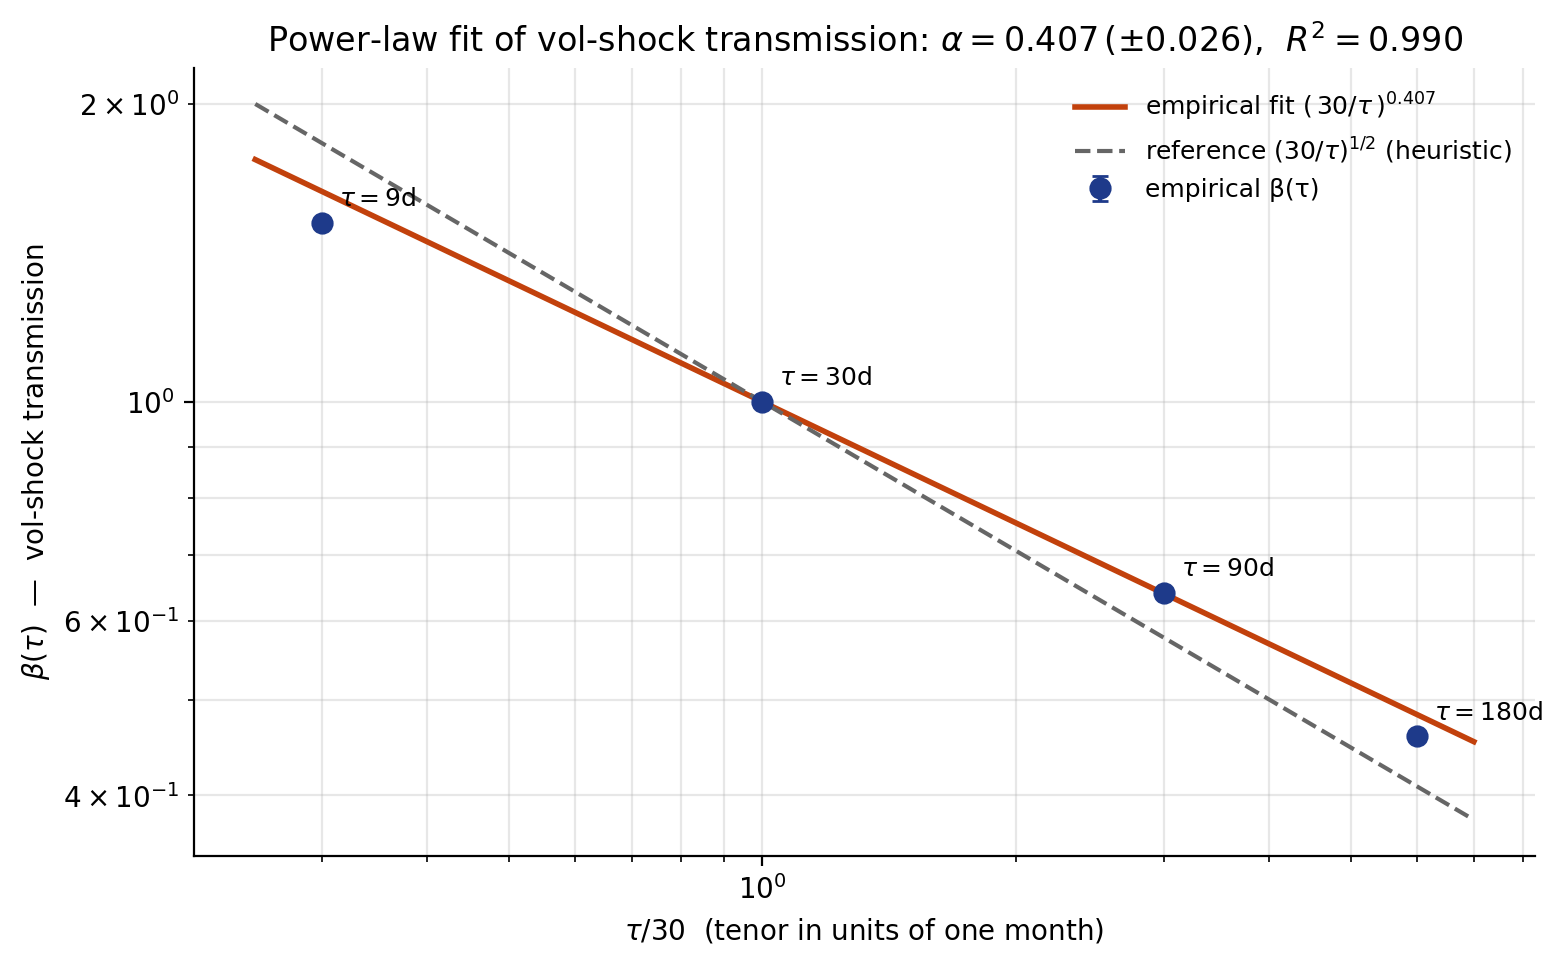
\includegraphics[keepaspectratio]{figures/ch7-vol-shock-powerlaw.png}}
\caption{Log-log of \(\beta(\tau)\) versus \(\tau/30\) with the
\(\sqrt{30/\tau}\) reference and the empirical \((30/\tau)^{0.41}\) fit}
\end{figure}

\emph{Log-log plot of \(\beta(\tau)\) against \(\tau/30\) for
\(\tau\in\{9, 30, 90,
180\}\). The dashed line is the heuristic \(\beta=\sqrt{30/\tau}\); the
solid line is the empirical fit \(\beta=(30/\tau)^{0.41}\). The
empirical line is visibly shallower: at \(\tau=180\) days the heuristic
predicts \(\beta=0.408\), the fit predicts \(0.483\), and the data give
\(0.459\) --- the fit is closer.}

A practical reading: under a 1-point shock to 30-day vol, the heuristic
says 6-month vol moves \(0.408\) points and the empirical exponent says
it moves \(0.483\) points --- an \(18\%\) correction in the same
direction. For a desk that runs the \(\sqrt{}\)-rule as gospel, the
implication is that the long-dated vega contribution to stress P\&L is
systematically \emph{understated} by close to one fifth.

\subsection{A.6 Regime dependence}\label{a.6-regime-dependence}

A single \(\hat\alpha\) for the whole 2011--2026 window averages over
very different volatility regimes. To check whether the rule is
regime-stable, roll a 60-day window of \(\beta(90)\) through the sample:
for each date \(t\), regress \(\Delta\sigma_{90}\) on
\(\Delta\sigma_{30}\) on the 60-day window ending at \(t\), and report
the slope.

\begin{figure}
\centering
\pandocbounded{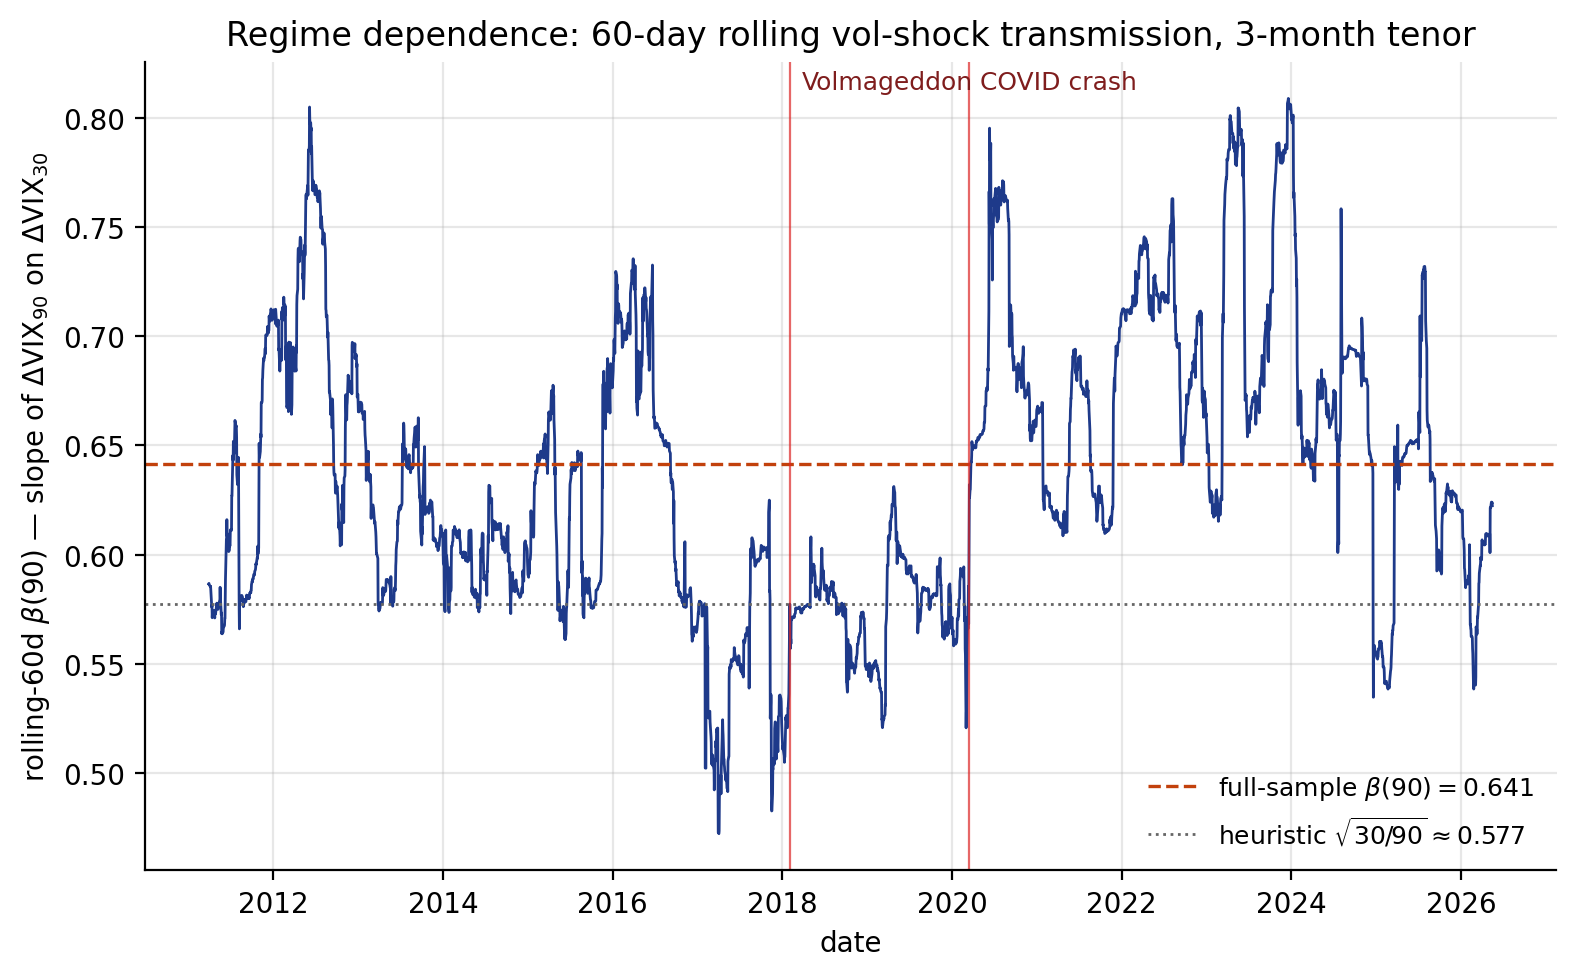
\includegraphics[keepaspectratio]{figures/ch7-vol-shock-regime.png}}
\caption{Rolling 60-day \(\beta(90)\) from 2011 through 2026, with
crisis windows annotated}
\end{figure}

\emph{Rolling 60-day OLS slope of \(\Delta\sigma_{90}\) on
\(\Delta\sigma_{30}\). Horizontal reference at \(\sqrt{30/90}=0.577\)
(the heuristic). Annotated windows: Feb 2018 Volmageddon (mean
\(\beta=0.575\) over \(\pm 60\) days, \(n=82\)); March 2020 COVID (mean
\(\beta=0.656\), \(n=84\)). The rolling series is rarely below the
heuristic for long.}

The distributional summary of the rolling series is

\[
\beta(90)_{\rm rolling}\;:\; \min = 0.472,\;\;
p_{10} = 0.564,\;\; \mathrm{median} = 0.627,\;\;
\mathrm{mean} = 0.636,\;\; p_{90} = 0.720,\;\; \max = 0.809. \tag{7.A7}
\]

The minimum occurred on 2017-04-03, deep in the long quiet post-Brexit
regime; the maximum on 2023-12-19, during the post-rate-hike
vol-compression. The heuristic value \(\sqrt{30/90}=0.577\) sits between
\(p_{10}\) and \(p_{20}\) of the rolling distribution. In other words:
on at least \(80\%\) of days the rule undershoots the local
\(\beta(90)\). The heuristic is not a centred estimate --- it is a
left-tail estimate.

Two crisis snapshots refine the picture. The February 2018 Volmageddon
window gives \(\beta(90)=0.575\) across \(\pm 60\) days --- the
heuristic value to three decimals. That was a \emph{front-localised}
shock: the inverse-VIX ETP unwind pushed VIX9D and VIX up while VIX3M
and VIX6M moved a fraction of that amount. The March 2020 COVID window
gives \(\beta(90)=0.656\), well above the heuristic --- a
\emph{curve-parallel} shock in which the entire surface re-priced to a
new macro regime. The two episodes bracket the rule in opposite
directions: no static exponent will capture both. In quiet regimes
\(\beta(90)\) drifts above the heuristic because long-dated vols track
the front in the absence of an event forcing the curve apart.

\subsection{A.7 Applying this to vega
risk}\label{a.7-applying-this-to-vega-risk}

Consider a worked example. A market-maker holds, after netting,
\(\$1\)mm of vega at the 30-day tenor, \(\$2\)mm at 90 days, and
\(\$4\)mm at 180 days --- a typical shape for a flow desk that writes
weekly product against long-dated portfolio hedges. The vega numbers are
in P\&L per vol point at each tenor. Under three competing stress
definitions of a ``1-vol shock'', the stress P\&L is

\[
\begin{aligned}
\text{Parallel:} \quad & \mathrm{PnL}\;=\; -(1+2+4)\,\text{mm} \;=\; -\$7.00\,\text{mm}, \\
\sqrt{30/\tau}\text{-rule:} \quad & \mathrm{PnL}\;=\; -(1\cdot 1 + 2\cdot 0.577 + 4\cdot 0.408)\,\text{mm} \;=\; -\$3.78\,\text{mm}, \\
\text{Empirical }(30/\tau)^{0.41}\text{:} \quad & \mathrm{PnL}\;=\; -(1\cdot 1 + 2\cdot 0.641 + 4\cdot 0.459)\,\text{mm} \;=\; -\$4.12\,\text{mm}.
\end{aligned} \tag{7.A8}
\]

The parallel shock overstates risk by \(\$2.9\)mm --- close to \(85\%\)
--- for this book shape. The \(\sqrt{}\)-rule undershoots the
empirically-correct number by \(\$0.34\)mm, or \(9\%\). Both errors are
large by absolute risk-budget standards, but the parallel shock is
\emph{order-of-magnitude} wrong while the \(\sqrt{}\)-rule is only a
calibration adjustment. A desk that runs the parallel shock will reject
reasonable positions because they look enormous; a desk that runs the
\(\sqrt{}\)-rule will be calibrated within \(10\%\) of truth on average.

The implication for vega bucketing (§7.3) is that the natural
representation of the vol stress is not a scalar --- it is a vector of
tenor-keyed shocks \(\{\delta\sigma_\tau\}_\tau\) tied together by a
fitted \(\beta\) function. Under empirical \(\alpha=0.41\), the shocks
for the four CBOE tenors per unit 30-day move are

\[
(\delta\sigma_9,\;\delta\sigma_{30},\;\delta\sigma_{90},\;\delta\sigma_{180}) \;=\; (1.52,\;1.00,\;0.64,\;0.46). \tag{7.A9}
\]

A vega risk number is then
\(\sum_\tau \mathcal V_\tau\,\delta\sigma_\tau\) with these weights. The
vega-bucketing system of §7.3.5 plugs into (7.A9) with the substitution
\(\mathcal V_\tau \mapsto \mathcal V_\tau\,
\delta\sigma_\tau\).

\subsection{A.8 Key takeaways}\label{a.8-key-takeaways}

\begin{enumerate}
\def\labelenumi{\arabic{enumi}.}
\item
  \textbf{A ``1-vol shock'' is ambiguous without a tenor convention.} A
  parallel shock and a \(\sqrt{30/\tau}\)-scaled shock differ by close
  to a factor of two on a realistic vega book. The convention is itself
  a risk-management choice and should be explicit on every risk report.
\item
  \textbf{The \(\sqrt{30/\tau}\) heuristic is theory-motivated.} Under
  any fast-mean-reverting volatility model --- log-OU or CIR (Heston)
  --- the term-IV response to an instantaneous variance shock decays as
  \(1/\sqrt{\tau}\) in the practitioner \(\tau\)-range of 30--180 days.
  The rule is not arbitrary.
\item
  \textbf{The empirical exponent is \(0.407 \pm 0.026\), not \(0.500\).}
  Across the 2011--2026 VIX-term-structure sample, a single-power-law
  fit gives \(\beta(\tau) = (30/\tau)^{0.407}\) with \(R^2 = 0.99\). The
  \(\sqrt{}\)-rule is rejected.
\item
  \textbf{The heuristic undershoots the back of the curve.} For 6-month
  vol it predicts \(\beta=0.408\) where the data give \(\beta=0.459\).
  Long-dated vols move \emph{more} than the \(\sqrt{}\)-rule claims when
  30-day vol shocks. A book that scales long-dated vega by the heuristic
  understates long-dated vol risk by \(10\)--\(20\%\).
\item
  \textbf{The heuristic overshoots the front.} For 9-day vol it predicts
  \(\beta=1.826\) where the data give \(\beta=1.517\). Weekly-option
  desks that bound front-vol stress by the \(\sqrt{}\)-rule are running
  a conservatively oversized stress test on the front of the surface.
\item
  \textbf{\(\beta(90)\) is regime-dependent.} Rolling 60-day
  \(\beta(90)\) ranges from \(0.47\) to \(0.81\) with mean \(0.64\). The
  heuristic value \(0.577\) sits near the \(20\)th percentile of the
  rolling distribution. In quiet regimes the back of the curve tracks
  the front more closely than the heuristic admits.
\item
  \textbf{Front-localised shocks differ from curve-parallel shocks.} The
  Feb 2018 Volmageddon window gave \(\beta(90)=0.575\) --- exactly the
  heuristic. The March 2020 COVID window gave \(\beta(90)=0.656\). The
  two episodes are equidistant from \(\beta=0.6\) in opposite
  directions. No static exponent will capture both.
\item
  \textbf{Vega bucketing is the operational fix.} Replace the scalar
  vega-stress number with a vector of tenor-keyed shocks tied by a
  fitted \(\beta(\tau)\) --- (7.A9) gives the empirically-calibrated
  weights for four standard tenors. The full Greek vector
  \((\Delta, \Gamma, \mathcal
  V_{9d}, \mathcal V_{30d}, \mathcal V_{90d}, \mathcal V_{180d}, \dots)\)
  is what a vega-risk system should report; the tenor-keyed
  decomposition is what the data support, not a single scalar
  \(\mathcal V\).
\end{enumerate}

\newpage

\chapter{Chapter 8 --- Forwards, Futures, and the Black
PDE}\label{chapter-8-forwards-futures-and-the-black-pde}

A European call on the December S\&P 500 futures looks identical to a
call on the spot index, but the pricing PDE loses its drift term, the
closed form drops a factor of \(e^{-rT}\), and the underlying dynamics
under \(\mathbb{Q}\) are driftless rather than GBM with drift \(r\). The
reason: \emph{entering a futures position costs nothing}.

This chapter consolidates the self-financing derivation of the Black
PDE, the parallel Feynman--Kac argument (Ch. 4), the Bachelier and OU
futures examples, the Margrabe exchange option (the cleanest two-asset
numeraire change in the guide), and the convexity adjustment between
futures and forwards under stochastic rates.

\textbf{Notation.} We write \(F_t(T)\) for both forward and futures,
distinguishing only when needed. Under deterministic rates they are
equal (§8.2); under stochastic rates they differ by the §8.11 convexity
adjustment. Sections 8.3--8.10 treat them interchangeably; only §8.11
separates them.

\begin{center}\rule{0.5\linewidth}{0.5pt}\end{center}

\section{8.1 Forward Price from a Zero-Cost
Claim}\label{forward-price-from-a-zero-cost-claim}

A \emph{forward contract} signed at time \(t\) with delivery at \(T\)
and strike \(K\) is the simplest possible derivative: an obligation to
exchange one unit of the underlying for the pre-agreed cash amount \(K\)
at maturity. Its terminal payoff is \(S_T - K\) for the long side and
\(K - S_T\) for the short side. By the risk-neutral pricing rule
developed in Chapter 6, its value at time \(t\) is

\[
\Pi_t \;=\; \mathbb{E}^{\mathbb{Q}}\!\left[\,e^{-r(T - t)}(S_T - K)\,\big|\,\mathcal{F}_t\right]. \tag{8.1}
\]

At signing, the strike \(K\) is chosen so that \(\Pi_t = 0\) --- neither
counterparty pays the other to enter. Setting (8.1) to zero and solving
\emph{under the constant-rate assumption},

\[
K \;=\; \mathbb{E}^{\mathbb{Q}}[\,S_T \mid \mathcal{F}_t\,] \;=\; S_t\,e^{r(T - t)}, \tag{8.2}
\]

where the second equality uses that \(S_t\,e^{-rt}\) is a
\(\mathbb{Q}\)-martingale under the bank-account numeraire (Chapter 5).
We call this \(K\) the \emph{forward price at time \(t\) for delivery at
\(T\)} and denote it \(F^{\text{fwd}}_t(T)\):

\[
F^{\text{fwd}}_t(T) \;=\; S_t\,e^{r(T - t)}. \tag{8.3}
\]

For continuous dividend yield \(\delta\),
\(F^{\text{fwd}}_t(T) = S_t e^{(r-\delta)(T-t)}\). As \(t \to T\),
\(F^{\text{fwd}}_t(T) \to S_T\).

Slope \(e^{(r-\delta)(T-t)}\): above 1 means \emph{contango} (forward
above spot, \(r > \delta\)), below 1 means \emph{backwardation}
(\(\delta > r\)). The sign drives commodity-derivative and
precious-metal strategies.

\textbf{Cash-and-carry.} No-\(\mathbb{Q}\) derivation: borrow \(S_t\) to
buy one share now (loan due \(S_t/P(t,T)\) at \(T\)) or sign a forward
(pay strike \(K\) at \(T\)). No-arbitrage forces

\[
F^{\text{fwd}}_t(T) \;=\; \frac{S_t}{P(t,T)}. \tag{8.4}
\]

Under constant rates this reduces to (8.3). The formula depends only on
spot and the discount bond --- not on volatility, drift, or any view.
The forward \emph{price} is a no-arbitrage number; the forward
\emph{value} of an existing contract with a stale strike depends on the
gap.

\pandocbounded{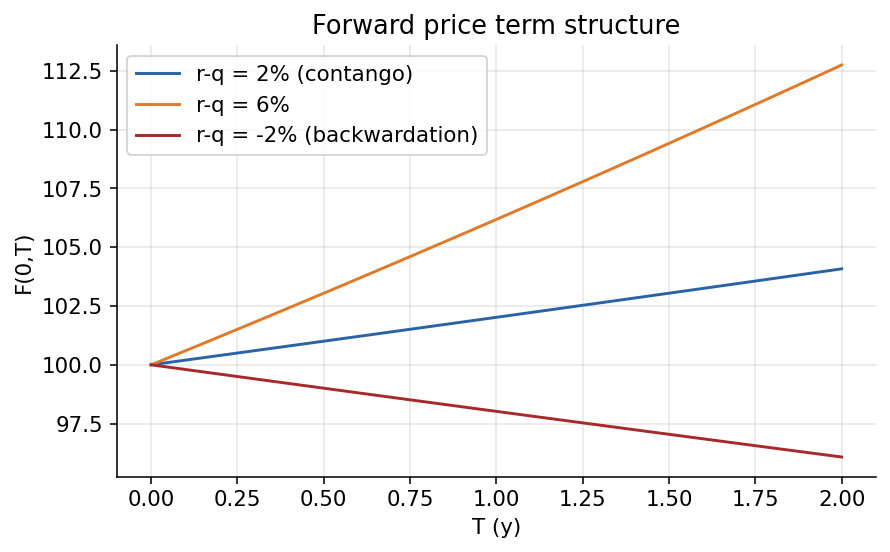
\includegraphics[keepaspectratio]{figures/ch08-forward-term.png}}
\emph{Forward price term structure --- cash-and-carry
\(F^{\text{fwd}}(t,T) = S_t/P(t,T)\) across maturities.}

\textbf{Forward price vs value.} The forward \emph{value} of an existing
contract with strike \(K_0\) is
\(\Pi_t = (F^{\text{fwd}}_t(T) - K_0) P(t, T)\); the forward
\emph{price} is the strike that makes a newly signed contract worth
zero. The market quotes the latter; mark-to-market produces the former.

Under the \(T\)-forward measure \(\mathbb{Q}^T\) with numeraire
\(P(t, T)\), the ratio \(S_t/P(t, T) = F^{\text{fwd}}_t(T)\) is a
martingale (Ch. 5 with \(A = P(\cdot, T)\), \(F = S\)). This is why
forwards admit Black-type formulas even under stochastic rates --- under
\(\mathbb{Q}^T\) the forward is driftless. Used heavily in Ch. 13 for
bond options.

\textbf{Cost of carry, generalised.} \(F^{\text{fwd}} = S/P\)
generalises to other asset classes by adjusting the carry leg:

{\def\LTcaptype{none} % do not increment counter
\begin{longtable}[]{@{}
  >{\raggedright\arraybackslash}p{(\linewidth - 4\tabcolsep) * \real{0.3333}}
  >{\raggedright\arraybackslash}p{(\linewidth - 4\tabcolsep) * \real{0.3333}}
  >{\raggedright\arraybackslash}p{(\linewidth - 4\tabcolsep) * \real{0.3333}}@{}}
\toprule\noalign{}
\begin{minipage}[b]{\linewidth}\raggedright
Asset class
\end{minipage} & \begin{minipage}[b]{\linewidth}\raggedright
Net yield / carry
\end{minipage} & \begin{minipage}[b]{\linewidth}\raggedright
Cash-and-carry forward
\end{minipage} \\
\midrule\noalign{}
\endhead
\bottomrule\noalign{}
\endlastfoot
Equity, dividend yield \(\delta\) & \(\delta\) &
\(S_t\,e^{(r - \delta)(T-t)}\) \\
FX, foreign rate \(r^f\) & \(r^f\) & \(S_t\,e^{(r - r^f)(T-t)}\)
(CIRP) \\
Commodity, conv-yield \(y\), storage \(u\) & \(y - u\) &
\(S_t\,e^{(r - y + u)(T-t)}\) \\
Income-generating asset, yield \(q\) & \(q\) &
\(S_t\,e^{(r - q)(T-t)}\) \\
\end{longtable}
}

In every case the \(\mathbb{Q}\)-drift is \(r - \text{(net yield)}\);
the formulas of §§8.5--8.11 apply uniformly with appropriate
substitution.

\begin{center}\rule{0.5\linewidth}{0.5pt}\end{center}

\section{8.2 Forwards vs.~Futures --- The Role of Daily
Settlement}\label{forwards-vs.-futures-the-role-of-daily-settlement}

Both are linear delta-one claims, both zero-sum at initiation, both have
delta \(\approx 1\). The difference: forwards settle at maturity,
futures settle daily. That small-looking gap drives different pricing
PDEs.

\textbf{The forward.} Payoff \(S_T - K\), time-\(t\) value

\[
\Pi_t \;=\; S_t \;-\; K\,P(t,T), \tag{8.5}
\]

--- asset leg \(S_t\) (\(\mathbb{Q}\)-martingale property), cash leg
\(-K P(t, T)\). P\&L accumulates unrealised on the balance sheet and
settles at maturity.

\textbf{The futures.} Daily settlement of \(\mathrm{d}F_t\) into a
margin account. Critically,

\[
\text{value of a futures position} \;\equiv\; 0, \tag{8.6}
\]

at every instant by design. Each \(\mathrm{d}F_t\) pays out as cash
immediately, so the holder's exposure is only to the next price change.
Cumulative P\&L from inception to \(t\) is \(F_t(T) - F_0(T)\).

The zero-value property is what makes futures clearable in size with
only margin, and what causes the option-pricing PDE to lose one term vs
Black--Scholes.

\textbf{Margin trace.} Four days, one-lot long:

{\def\LTcaptype{none} % do not increment counter
\begin{longtable}[]{@{}lllll@{}}
\toprule\noalign{}
\(t\) & \(F_t(T)\) & \(\Delta F\) & Margin cash flow & Cumulative
margin \\
\midrule\noalign{}
\endhead
\bottomrule\noalign{}
\endlastfoot
0 & 100 & --- & 0 & 0 \\
1 & 101 & +1 & +1 & +1 \\
2 & 103 & +2 & +2 & +3 \\
3 & 99 & -4 & -4 & -1 \\
\end{longtable}
}

Cumulative margin is always \(F_t - F_0\) --- the mark-to-market
invariant. Continuously, \(\int_0^t \mathrm{d}F_s = F_t - F_0\).

Under deterministic rates, forward and futures economics are identical:
PV of a cash stream equals PV of a maturity payment when
borrowing/lending at \(r\) is frictionless. Under stochastic rates, the
daily margin earns interest at a stochastic rate that may correlate with
\(S\) --- opening the convexity gap of §8.11.

\begin{center}\rule{0.5\linewidth}{0.5pt}\end{center}

\section{\texorpdfstring{8.3 The Futures Price as a
\(\mathbb{Q}\)-Martingale}{8.3 The Futures Price as a \textbackslash mathbb\{Q\}-Martingale}}\label{the-futures-price-as-a-mathbbq-martingale}

The futures price itself is a \(\mathbb{Q}\)-martingale. The argument is
tautological given (8.6): a costless position must have zero expected
P\&L under \(\mathbb{Q}\), otherwise free option:

\[
\mathbb{E}^{\mathbb{Q}}\!\left[\,F_{t^+}(T) - F_t(T)\mid \mathcal{F}_t\,\right] \;=\; 0. \tag{8.7}
\]

Equivalently, for all \(s \le t\),

\[
\boxed{\;\mathbb{E}^{\mathbb{Q}}\!\bigl[F_t(T) \mid \mathcal{F}_s\bigr] \;=\; F_s(T)\;} \tag{8.8}
\]

--- the futures price is a \(\mathbb{Q}\)-martingale.

\textbf{A trio of drifts.} It is worth lining up the three kinds of
asset that appear in this guide and noting the drift each of them takes
under \(\mathbb{Q}\):

{\def\LTcaptype{none} % do not increment counter
\begin{longtable}[]{@{}
  >{\raggedright\arraybackslash}p{(\linewidth - 4\tabcolsep) * \real{0.3333}}
  >{\raggedright\arraybackslash}p{(\linewidth - 4\tabcolsep) * \real{0.3333}}
  >{\raggedright\arraybackslash}p{(\linewidth - 4\tabcolsep) * \real{0.3333}}@{}}
\toprule\noalign{}
\begin{minipage}[b]{\linewidth}\raggedright
Asset type
\end{minipage} & \begin{minipage}[b]{\linewidth}\raggedright
\(\mathbb{Q}\)-drift
\end{minipage} & \begin{minipage}[b]{\linewidth}\raggedright
Reason
\end{minipage} \\
\midrule\noalign{}
\endhead
\bottomrule\noalign{}
\endlastfoot
\emph{Traded asset} (e.g.~a non-dividend stock) & \(r\,X_t\) &
Discounted price \(X_t/M_t\) is a \(\mathbb{Q}\)-martingale; carry at
\(r\) \\
\emph{Traded asset with yield \(\delta\)} & \((r - \delta)\,X_t\) &
Discounted total return (price + dividends) is a
\(\mathbb{Q}\)-martingale \\
\emph{Futures quote} \(F_t(T)\) & \(0\) & Position is costless; expected
change under \(\mathbb{Q}\) is zero \\
\emph{Non-traded variable} (e.g.~temperature) &
\(\mu^{\mathbb{Q}}_t - \sigma_t\,\lambda_t\) & Needs a market price of
risk \(\lambda_t\) (Chapter 6) \\
\end{longtable}
}

The first three rows are pinned by replication arguments. The fourth
requires additional market information --- a market price of risk ---
because there is no hedgeable instrument that pins the drift. For the
rest of this chapter, the futures price is the canonical example of row
3.

\textbf{Forward prices are different.} Contrast (8.8) with the analogous
statement for a \emph{forward} price
\(F^{\text{fwd}}_t(T) = S_t/P(t,T)\). Under \(\mathbb{Q}\) (bank-account
numeraire), \(F^{\text{fwd}}_t(T)\) is \emph{not} a martingale in
general --- both \(S_t\) and \(1/P(t,T)\) drift, and their ratio drifts.
The cleanest statement is instead that \(F^{\text{fwd}}_t(T)\) is a
\(\mathbb{Q}^T\)-martingale, where \(\mathbb{Q}^T\) is the \(T\)-forward
measure with numeraire \(P(\cdot, T)\). This follows from the general
numeraire identity of Chapter 5: if \(A\) is a traded numeraire, every
traded asset divided by \(A\) is a \(\mathbb{Q}^A\)-martingale, and
\(S_t / P(t,T)\) is precisely such a ratio. Futures and forwards
therefore live in \emph{different measures}: the futures price is
naturally a \(\mathbb{Q}\)-martingale, the forward price is naturally a
\(\mathbb{Q}^T\)-martingale. Under deterministic rates the two measures
coincide (their Radon--Nikodym density collapses to 1), so futures and
forwards coincide; under stochastic rates they diverge and the gap is
the convexity adjustment of §8.11.

\textbf{A subtle point about ``the futures is undiscounted''.} It is
tempting to read (8.8) as saying the futures \emph{price} requires no
discounting. That is correct. But an \emph{option on a futures} ---
whose cash payoff settles at some maturity \(T_0\) --- is an ordinary
traded derivative whose cash payoff must be discounted back to today in
the usual way. The common pitfall is to conflate the two: the futures
\emph{quote} has no drift under \(\mathbb{Q}\), but the option's
\emph{value} still carries the usual discount factor \(e^{-r(T_0-t)}\).
The Black '76 formula in §8.7 will make this explicit.

\begin{center}\rule{0.5\linewidth}{0.5pt}\end{center}

\section{\texorpdfstring{8.4 Dynamics of the Futures Price Under
\(\mathbb{Q}\)}{8.4 Dynamics of the Futures Price Under \textbackslash mathbb\{Q\}}}\label{dynamics-of-the-futures-price-under-mathbbq}

The martingale property (8.8) fixes the \(\mathbb{Q}\)-drift of
\(F_t(T)\) at zero, but leaves the volatility unspecified. Different
market settings motivate different volatility parameterisations. We
postulate a general form

\[
\mathrm{d}F_t(T) \;=\; \sigma^F(t, F_t(T))\,\mathrm{d}\widehat{W}_t \qquad (\mathbb{Q}\text{-measure}), \tag{8.9}
\]

with \(\widehat{W}\) a \(\mathbb{Q}\)-Brownian motion. The specific
functional form of \(\sigma^F(t, F)\) is a modelling choice:

\begin{itemize}
\tightlist
\item
  \textbf{GBM.} \(\sigma^F(t, F) = \sigma\,F\) yields the log-normal
  Black '76 model of §8.7, which is the market standard for equity-index
  futures, FX forwards, and commodity-futures implied-volatility
  quotation.
\item
  \textbf{Bachelier (arithmetic).} \(\sigma^F(t, F) = \sigma\)
  (constant) yields the arithmetic-Brownian model of §8.8, appropriate
  when \(F\) can go negative --- interest-rate futures near the zero
  bound, or crude-oil futures during the April 2020 episode.
\item
  \textbf{Samuelson / OU.} \(\sigma^F(t, F) = \sigma\,e^{-\eta(T - t)}\)
  yields a mean-reverting arithmetic model where the vol loading
  \emph{decays} as one looks further forward in the curve --- matching
  the empirical fact that long-dated commodity futures move less in
  absolute terms than front-month ones (§8.9).
\end{itemize}

\textbf{Derivation under constant rates.} For the GBM case it is worth
showing that (8.9) with \(\sigma^F = \sigma F\) falls out of the spot
dynamics plus the cost-of-carry identity. Suppose the spot satisfies

\[
\frac{\mathrm{d}S_t}{S_t} \;=\; \mu\,\mathrm{d}t \;+\; \sigma\,\mathrm{d}W_t \qquad (\mathbb{P}), \tag{8.10}
\]

and constant rates \(r\) apply. The forward/futures price is \(F_t(T) =
S_t\,e^{r(T-t)}\). By Itô on \(f(t, S) = S\,e^{r(T-t)}\),

\[
\mathrm{d}F_t(T) \;=\; e^{r(T-t)}\,\mathrm{d}S_t \;-\; r\,S_t\,e^{r(T-t)}\,\mathrm{d}t. \tag{8.11}
\]

Expanding
\(\mathrm{d}S_t = \mu S_t\,\mathrm{d}t + \sigma S_t\,\mathrm{d}W_t\) and
using \(F_t = S_t\,e^{r(T-t)}\),

\[
\frac{\mathrm{d}F_t(T)}{F_t(T)} \;=\; (\mu - r)\,\mathrm{d}t \;+\; \sigma\,\mathrm{d}W_t \qquad (\mathbb{P}). \tag{8.12}
\]

Under the risk-neutral measure \(\mathbb{Q}\), the stock's drift is
\(\mu = r\) (Chapter 6, market-price-of-risk argument). Substituting,

\[
\boxed{\;\frac{\mathrm{d}F_t(T)}{F_t(T)} \;=\; \sigma\,\mathrm{d}\widehat{W}_t \qquad (\mathbb{Q}).\;} \tag{8.13}
\]

The drift \((\mu - r)\,\mathrm{d}t\) in (8.12) is exactly cancelled
under \(\mathbb{Q}\) by the measure change
\(\mathrm{d}W_t \to \mathrm{d}\widehat{W}_t
+ \lambda\,\mathrm{d}t\) with \(\lambda = (\mu - r)/\sigma\) (Girsanov,
Chapter 5). The drift \((\mu - r)\) gets killed; the diffusion
\(\sigma\) survives. This is the martingale property (8.8) made explicit
at the SDE level. Every drift term in the spot SDE --- whether from
physical-world mean-reversion, from the cost of carry \(r\), or from a
dividend yield --- is absorbed into the futures quote or vanishes under
\(\mathbb{Q}\); what survives on the futures is only the diffusion term.

\textbf{Case with dividends.} If the stock pays a continuous yield
\(\delta\), the spot drifts at \(r - \delta\) under \(\mathbb{Q}\), and
the cost-of-carry formula becomes \(F_t(T) = S_t\,e^{(r-\delta)(T-t)}\).
Applying Itô's product rule to \(F_t = S_t\,g(t)\) with
\(g(t) = e^{(r-\delta)(T-t)}\), \(g'(t) = -(r-\delta) g(t)\):

\[
\begin{aligned}
\mathrm{d}F_t &= g(t)\,\mathrm{d}S_t + S_t\,g'(t)\,\mathrm{d}t \\
&= g(t) S_t\!\left[(r-\delta)\,\mathrm{d}t + \sigma\,\mathrm{d}\widehat{W}_t\right] - (r-\delta) g(t) S_t\,\mathrm{d}t \\
&= \sigma\,g(t) S_t\,\mathrm{d}\widehat{W}_t = \sigma F_t\,\mathrm{d}\widehat{W}_t,
\end{aligned}
\]

so

\[
\boxed{\;\frac{\mathrm{d}F_t(T)}{F_t(T)} \;=\; \sigma\,\mathrm{d}\widehat{W}_t \qquad (\mathbb{Q})\;}.
\]

The \((r-\delta)\)-drift of the spot exactly cancels the time-decay of
the carry factor: \(F\) is a \(\mathbb{Q}\)-martingale even with
dividends, as the FTAP on futures (8.8) demands. This is the general
principle --- any continuous yield or cost-of-carry term that affects
the spot under \(\mathbb{Q}\) gets absorbed into the forward's
deterministic drift and cancels, leaving pure diffusion on the
forward/futures quote.

\textbf{General dynamics.} For modelling purposes, we often write (8.9)
with a general state- and time-dependent volatility \(\sigma^F(t, F)\):

\[
\mathrm{d}F_t(T) \;=\; \sigma^F(t, F_t(T))\,\mathrm{d}\widehat{W}_t. \tag{8.14}
\]

All the machinery of the next three sections works at this level of
generality: the Black PDE, its Feynman--Kac representation, and the
closed-forms for specific choices of \(\sigma^F\) are all instances of
(8.14).

\begin{center}\rule{0.5\linewidth}{0.5pt}\end{center}

\section{8.5 Black PDE for options on
futures}\label{black-pde-for-options-on-futures}

A European option on futures has terminal payoff

\[
g_{T_0} \;=\; \varphi\!\big(F_{T_0}(T)\big), \tag{8.15}
\]

with \(T_0\) the option exercise and \(T \ge T_0\) the futures delivery
(typically equal). Because \(F\) is a \(\mathbb{Q}\)-martingale the PDE
loses its first-derivative drift. Two derivations: self-financing, and
Feynman--Kac.

\subsection{8.5.1 Setup of the replicating
portfolio}\label{setup-of-the-replicating-portfolio}

Let \(g_t = g(t, F_t(T))\). Form

\[
V_t \;=\; \alpha_t\,F_t(T) \;+\; \beta_t\,B_t \;-\; g_t, \tag{8.16}
\]

\(\alpha_t\) futures contracts (zero cost --- notional only),
\(\beta_t\) cash, \(V_0 = 0\). Futures P\&L comes entirely from
\(\alpha_t \mathrm{d}F_t\).

\subsection{8.5.2 Self-financing
increment}\label{self-financing-increment}

The wealth change is

\[
\mathrm{d}V_t \;=\; \alpha_t\,\mathrm{d}F_t(T) \;+\; \beta_t\,\mathrm{d}B_t \;-\; \mathrm{d}g_t. \tag{8.18}
\]

Expanding via Itô on \(g(t, F)\) and using the driftless dynamics of
\(F\) under \(\mathbb{Q}\),

\[
\mathrm{d}g_t \;=\; \left[\partial_t g \;+\; \tfrac12 (\sigma^F)^2\,\partial_{FF} g\right]\mathrm{d}t \;+\; \sigma^F\,\partial_F g\,\mathrm{d}\widehat{W}_t, \tag{8.19}
\]

so

\[
\mathrm{d}V_t \;=\; \alpha_t\,\sigma^F\,\mathrm{d}\widehat{W}_t \;+\; \beta_t\,r\,B_t\,\mathrm{d}t \;-\; \left[\partial_t g + \tfrac12 (\sigma^F)^2\,\partial_{FF} g\right]\mathrm{d}t \;-\; \sigma^F\,\partial_F g\,\mathrm{d}\widehat{W}_t. \tag{8.20}
\]

\subsection{8.5.3 Eliminating noise and
drift}\label{eliminating-noise-and-drift}

The \(\mathrm d\widehat W\) coefficient vanishes iff

\[
\boxed{\;\alpha_t \;=\; \partial_F g(t, F_t(T)),\;} \tag{8.21}
\]

the \emph{futures-delta} hedge --- \(\partial_F g\) units of futures
notional per option short. With \(\alpha_t = \partial_F g\) imposed, the
\(\mathrm dt\) coefficient in (8.20) is

\[
\mathcal{A}_t \;=\; \beta_t\,r\,B_t \;-\; \partial_t g \;-\; \tfrac12 (\sigma^F)^2\,\partial_{FF} g. \tag{8.22}
\]

From \(V_t \equiv 0\) and the zero-value feature of the futures
position, \(\beta_t\,B_t = g_t\), so \(\beta_t r B_t = r\,g_t\) (eq
8.23). Setting \(\mathcal A_t = 0\) then yields the \emph{Black PDE for
options on futures}:

\subsection{8.5.4 The PDE}\label{the-pde}

\[
\boxed{\;\partial_t g \;+\; \tfrac12\,(\sigma^F(t, F))^2\,\partial_{FF} g \;=\; r\,g, \qquad g(T_0, F) = \varphi(F).\;} \tag{8.24}
\]

Compared to the BS PDE for a stock,

\[
\partial_t g \;+\; r\,S\,\partial_S g \;+\; \tfrac12\,\sigma^2 S^2\,\partial_{SS} g \;=\; r\,g,
\]

the drift \(r S \partial_S g\) has disappeared --- the signature of
pricing off a \(\mathbb{Q}\)-martingale. The \(r g\) on the right is
still the discount on the option's cash payoff at \(T_0\). For
\(\sigma^F(t, F) = \sigma F\) this becomes

\[
\partial_t g \;+\; \tfrac12\,\sigma^2\,F^2\,\partial_{FF} g \;=\; r\,g, \qquad g(T_0, F) = \varphi(F), \tag{8.25}
\]

the PDE that the Black '76 formula of §8.7 solves.

\subsection{8.5.5 Feynman--Kac
representation}\label{feynmankac-representation}

Applying Feynman--Kac (Chapter 4) to (8.24) gives the cross-check

\[
\boxed{\;g(t, F) \;=\; \mathbb{E}^{\mathbb{Q}}\!\left[\,e^{-r(T_0 - t)}\,\varphi(F_{T_0}(T))\;\Big|\;F_t(T) = F\,\right],\;} \tag{8.26}
\]

with \(F_u\) driftless under \(\mathbb{Q}\). Two differences from the
stock-BS expectation: zero drift (not \(r\)), and \(e^{-r(T_0-t)}\) on
the payoff (cash settles at \(T_0\)). Under stochastic rates the
forward-measure variant

\[
\frac{g(t, F)}{P(t, T_0)} \;=\; \mathbb{E}^{\mathbb{Q}^{T_0}}\!\left[\,\varphi(F_{T_0}(T))\,\big|\,F_t(T) = F\,\right] \tag{8.27}
\]

is the cleaner starting point (Ch. 13). Integrating (8.14) gives the GBM
and Bachelier marginals:

\[
F_{T_0}(T) \;=\; F_t(T)\,\exp\!\left\{-\tfrac12 \sigma^2 (T_0 - t) + \sigma\,(\widehat{W}_{T_0} - \widehat{W}_t)\right\} \tag{8.28}
\]

for the log-normal case \(\sigma^F = \sigma F\), and

\[
F_{T_0}(T) \;=\; F_t(T) \;+\; \sigma\,(\widehat{W}_{T_0} - \widehat{W}_t) \tag{8.29}
\]

for Bachelier \(\sigma^F = \sigma\). In both cases
\(\mathbb E^{\mathbb Q}[F_{T_0}(T)\mid \mathcal F_t] = F_t(T)\),
restating the martingale property (8.8).

\begin{center}\rule{0.5\linewidth}{0.5pt}\end{center}

\section{8.7 The Black '76 Closed Form}\label{the-black-76-closed-form}

For the constant-volatility GBM case \(\sigma^F(t, F) = \sigma F\) with
payoff \(\varphi(F) = (F - K)_+\), the PDE (8.25) admits the celebrated
\emph{Black '76} closed-form solution:

\[
\boxed{\;g(t, F) \;=\; e^{-r(T_0 - t)}\!\left[\,F\,\Phi(d_+) \;-\; K\,\Phi(d_-)\,\right],\;} \tag{8.30}
\]

with

\[
d_\pm \;=\; \frac{\ln(F/K) \;\pm\; \tfrac12\,\sigma^2\,(T_0 - t)}{\sigma\,\sqrt{T_0 - t}}. \tag{8.31}
\]

\textbf{Derivation via Feynman--Kac.} Starting from (8.26) with
\(\varphi(F) =
(F - K)_+\) and the log-normal law (8.28):

\[
g(t, F) \;=\; e^{-r(T_0 - t)}\,\mathbb{E}^{\mathbb{Q}}\!\left[\,(F_{T_0}(T) - K)_+ \mid F_t(T) = F\,\right].
\]

The expectation is the classical log-normal ``call-option'' integral,
and the log-variance is \(\sigma^2(T_0 - t)\) with log-mean
\(\ln F - \tfrac12 \sigma^2
(T_0 - t)\). A direct Gaussian computation gives

\[
\mathbb{E}^{\mathbb{Q}}\!\left[(F_{T_0} - K)_+ \mid F_t = F\right] \;=\; F\,\Phi(d_+) \;-\; K\,\Phi(d_-),
\]

and multiplying by the discount \(e^{-r(T_0 - t)}\) yields (8.30).

\textbf{Comparison to Black--Scholes.} The standard BS formula on a
non-dividend stock is

\[
C^{\text{BS}}(S, K, r, \sigma, \tau) \;=\; S\,\Phi(d_1) \;-\; K\,e^{-r\tau}\,\Phi(d_2),
\]

with
\(d_{1,2} = [\ln(S/K) + (r \pm \tfrac12 \sigma^2)\tau]/(\sigma\sqrt{\tau})\).
The Black '76 formula (8.30) differs in two readable ways:

{\def\LTcaptype{none} % do not increment counter
\begin{longtable}[]{@{}lll@{}}
\toprule\noalign{}
& Black--Scholes (spot) & Black '76 (futures) \\
\midrule\noalign{}
\endhead
\bottomrule\noalign{}
\endlastfoot
``Moneyness'' in \(d_\pm\) & \(\ln(S/K) + r\tau\) & \(\ln(F/K)\) only \\
Coefficient on \(\Phi(d_+)\) & \(S\) & \(e^{-r\tau}\,F\) \\
Coefficient on \(\Phi(d_-)\) & \(K\,e^{-r\tau}\) & \(e^{-r\tau}\,K\) \\
\end{longtable}
}

The first change reflects the absence of a first-derivative drift term
in the Black PDE --- the ``cost of carry'' \(r\tau\) that shifts the
moneyness in BS does not appear in Black '76 because the underlying is
already a martingale. The second change reflects that the futures quote
\(F\) is itself undiscounted; to state the option price as a dollar
amount today, we simply discount the whole expression by \(e^{-r\tau}\).

\textbf{Three observations.} (8.30) is BS with spot replaced by forward
and the drift shift dropped. The dividend yield does not appear --- it
is absorbed into \(F\). Plugging \(F_t(T) = S_t e^{(r-\delta)(T-t)}\)
recovers the dividend-BS formula exactly.

Pitfall: the discount factor is \(e^{-r(T_0 - t)}\), not \(e^{-r(T-t)}\)
--- option maturity, not futures delivery. They coincide on standard
exchange products but can differ by months on mid-curve options.

Black '76 delta:

\[
\partial_F g \;=\; e^{-r(T_0 - t)}\,\Phi(d_+). \tag{8.32}
\]

vs the BS spot delta \(\Phi(d_1)\) --- the Black '76 delta carries an
extra discount. Hedge \(e^{-r(T_0-t)} \Phi(d_+)\) futures per option
short. Negligible at short tenors, material on multi-year contracts.

\textbf{Black '76 Greeks} (with \(\tau = T_0 - t\), \(\phi\) the
standard-normal PDF):

\[
\begin{aligned}
\Delta \;&=\; \partial_F g \;=\; e^{-r\tau}\,\Phi(d_+), \\
\Gamma \;&=\; \partial_{FF} g \;=\; \frac{e^{-r\tau}\,\phi(d_+)}{F\,\sigma\,\sqrt{\tau}}, \\
\text{Vega} \;&=\; \partial_\sigma g \;=\; e^{-r\tau}\,F\,\phi(d_+)\,\sqrt{\tau}, \\
\Theta \;&=\; \partial_t g \;=\; -\frac{e^{-r\tau}\,F\,\phi(d_+)\,\sigma}{2\sqrt{\tau}} \;+\; r\,e^{-r\tau}\,[F\,\Phi(d_+) - K\,\Phi(d_-)], \\
\rho \;&=\; \partial_r g \;=\; -\tau\,g(t, F).
\end{aligned}
\]

Gamma carries an extra \(e^{-r\tau}\) vs BS. Rho is \emph{negative} on a
Black '76 call (rate hike discounts the cash payoff more heavily),
whereas BS-spot rho is positive --- a clean diagnostic for whether a
pricing engine treats a contract as spot or futures.

\textbf{Numeric.} \(F = K = 100\), \(\sigma = 20\%\), \(\tau = 0.25\),
\(r = 5\%\). \(d_+ = 0.05\), \(d_- = -0.05\),
\(\Phi(\pm 0.05) \approx 0.5199 / 0.4801\). Black '76 price:

\[
g \;=\; e^{-0.05\cdot 0.25}\,[100 \cdot 0.5199 - 100 \cdot 0.4801] \;\approx\; 0.9876 \cdot 3.98 \;\approx\; 3.93.
\]

The analogous BS spot call (same parameters) gives \(\approx 4.62\) ---
higher than Black '76 because the spot drifts at \(r > 0\) under
\(\mathbb{Q}\) while the futures is a martingale. The difference is the
drift term cumulating over \(\tau\).

\textbf{Why Black is ubiquitous.} Beyond literal futures options, Black
'76 prices caps, floors, swaptions (Ch. 14), commodity-forward options,
and ATM options on forward yield curves. The mechanism is always the
same: any underlying that is a martingale under \emph{some} numeraire
reduces the PDE to (8.25). In the LIBOR/SOFR caplet setting,
\(L(t, T_1, T_2)\) is a martingale under the \(T_2\)-forward measure and
the caplet price is Black '76 with \(F = L\).

\pandocbounded{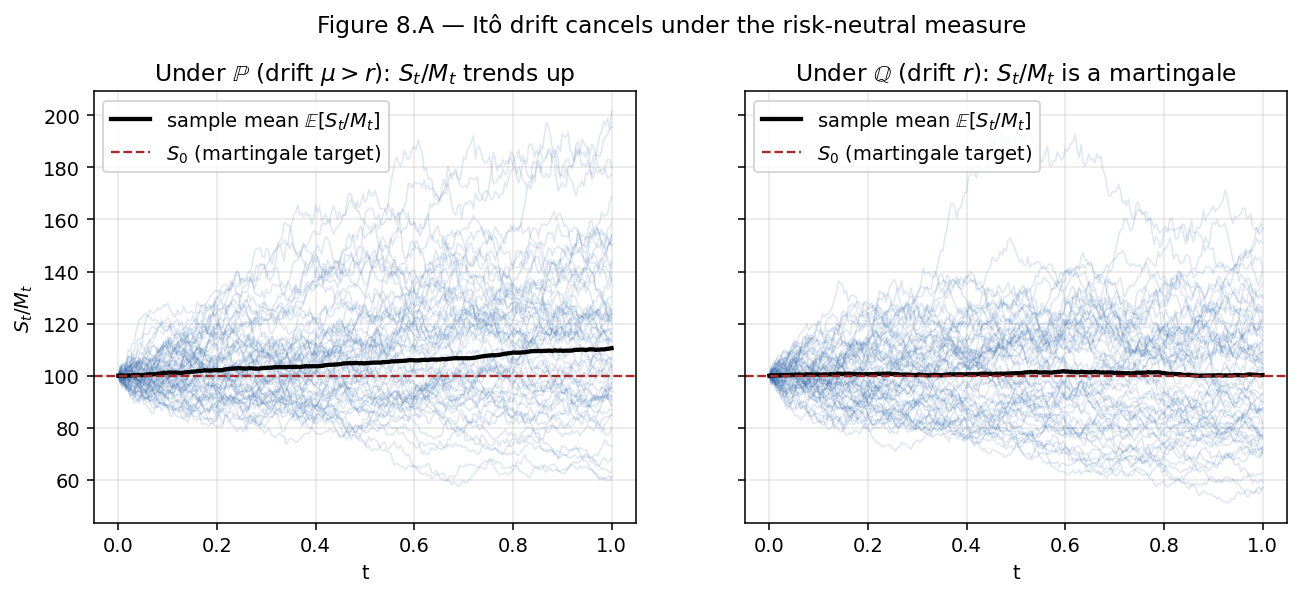
\includegraphics[keepaspectratio]{figures/ch08-drift-cancel.png}}
\emph{Drift-cancel schematic --- the first-derivative drift term in the
Black PDE vanishes because the futures is a \(\mathbb{Q}\)-martingale,
leaving only the second-derivative diffusion.}

\begin{center}\rule{0.5\linewidth}{0.5pt}\end{center}

\section{8.8 Example --- Bachelier Futures and the Arithmetic
Binary}\label{example-bachelier-futures-and-the-arithmetic-binary}

The Bachelier model has constant \emph{absolute} volatility, no drift
--- the natural choice for underlyings that can go negative (short-rate
futures near zero, the April 2020 crude episode). It isolates the
martingale pricing approach from the mechanics of log-normal
integration, which is pedagogically useful.

Take

\[
\mathrm{d}F_t \;=\; \sigma\,\mathrm{d}\widehat{W}_t \qquad (\mathbb{Q}), \tag{8.33}
\]

with constant absolute volatility \(\sigma\), and consider a
\emph{binary call}

\[
\varphi(F) \;=\; \mathbf{1}_{\{F > K\}}
\]

--- the claim pays 1 unit if the futures is above \(K\) at option expiry
\(T_0\), zero otherwise. For simplicity we take \(r = 0\) in this
example so that no discount factor clutters the formula; the general
\(r \neq 0\) result multiplies the answer by \(e^{-r(T_0 - t)}\).

\subsection{8.8.1 Terminal distribution}\label{terminal-distribution}

From (8.33),

\[
F_{T_0} - F_t \;=\; \sigma\,(\widehat{W}_{T_0} - \widehat{W}_t), \qquad \widehat{W}_{T_0} - \widehat{W}_t \stackrel{d}{=} \mathcal{N}(0, T_0 - t), \tag{8.34}
\]

so \(F_{T_0}\) is conditionally normal with mean \(F_t\) (the martingale
property) and variance \(\sigma^2\,(T_0 - t)\).

\subsection{8.8.2 Pricing}\label{pricing}

By Feynman--Kac (8.26) with \(r = 0\),

\[
h(t, F) \;=\; \mathbb{E}^{\mathbb{Q}}_{t, F}\!\left[\,\mathbf{1}_{\{F_{T_0} > K\}}\,\right] \;=\; \mathbb{Q}_{t, F}\bigl(F_{T_0} > K\bigr). \tag{8.35}
\]

Writing \(F_{T_0} - F_t = \sigma\,(\widehat{W}_{T_0} - \widehat{W}_t)\)
and letting \(Z \sim \mathcal{N}(0, 1)\),

\[
h(t, F) \;=\; \mathbb{Q}\!\left(Z \;>\; \frac{K - F}{\sigma\,\sqrt{T_0 - t}}\right) \;=\; \Phi\!\left(\frac{F - K}{\sigma\,\sqrt{T_0 - t}}\right), \tag{8.36}
\]

with \(\Phi\) the standard-normal CDF. (For the historically-rooted
version using \(\sigma = 2\) that appears in the draft, one simply
substitutes \(\sigma = 2\) into (8.36).)

\subsection{8.8.3 Reading the answer}\label{reading-the-answer}

The argument of \(\Phi\) in (8.36) is a \emph{\(z\)-score}: \((F-K)\) in
units of the remaining standard deviation \(\sigma\sqrt{T_0-t}\). The
price of the digital is the probability that a standard normal exceeds
\(-z\). At the money (\(F = K\)), \(\Phi(0) = 1/2\) exactly --- a
symmetry unique to the arithmetic model. Under \(r \ne 0\), discount the
dollar payoff:
\(h(t,F) = e^{-r(T_0-t)}\,\Phi((F-K)/(\sigma\sqrt{T_0-t}))\). Terminal
limit \(T_0 \to t\) collapses \(\Phi\) to \(\mathbf 1_{\{F>K\}}\),
matching the payoff.

\subsection{8.8.4 Case study: Negative WTI futures, April 20 2020 ---
when lognormal
breaks}\label{case-study-negative-wti-futures-april-20-2020-when-lognormal-breaks}

\emph{Storage at Cushing was full; longs had to pay to take delivery.}
\emph{Black-76's \(\ln F\) is undefined at \(F\le 0\); Bachelier's
\(\mathbb R\)-support is.} \emph{CME switched the official option model
from Black-76 to Bachelier the same week.}

\textbf{Context.} On Monday 20 April 2020, the front-month NYMEX WTI
crude futures (May 2020 contract, CL K20) settled at \emph{minus}
\$37.63 per barrel --- the first negative settle in the history of the
contract. With physical delivery at Cushing, Oklahoma scheduled for May
21 and storage there saturated by collapsed COVID-era demand, holders of
long expiring futures discovered they would have to \emph{pay} to take
delivery. Through the day the contract traded from +\$18 to −\$40; CME
had reprogrammed its trade-matching engine on Friday 17 April explicitly
to accept negative prices, after a research notice flagged that the
legacy Black-76 pricing engines could not quote options on a contract
that might cross zero.

The market structure on the day made the move worse. Open interest in
the May contract was still \textasciitilde108k lots heading into the
final settlement window with three trading days to expiry --- unusual:
by convention the front-month contract rolls down to a few thousand lots
before notice. The overhang was substantially held by long-only
commodity ETFs (notably the United States Oil Fund, USO, which alone
held \textasciitilde25\% of front-month OI in mid-April) that were
structurally unable to take delivery. Forced rolling into a non-buyer
market produced a price discovery process that was about storage
logistics, not about the consensus value of a barrel of oil.

\textbf{Through the chapter's math.} Black-76 (8.30) requires \(F > 0\)
because the lognormal SDE (8.13),
\(\mathrm dF/F = \sigma\,\mathrm d\widehat W\), has an absorbing barrier
at zero --- log-prices are not defined for \(F \le
0\) and the formula for \(d_\pm\) contains \(\ln(F/K)\), which is
singular. Bachelier dynamics (8.34),
\(\mathrm dF = \sigma\,\mathrm d\widehat W\), are defined on all of
\(\mathbb R\): the terminal distribution (8.29) is normal with mean
\(F_t\), so negative outcomes are admissible and the binary call (8.36)
is well-defined at every \(F\). The choice of model is not decorative
--- it determines which prices are even \emph{expressible}. CME formally
switched the official option-pricing methodology for WTI and several
refined-product contracts from Black-76 to Bachelier on Friday 22 April
2020 (Special Executive Report S-8520). By April 2020 every major
commodity desk had migrated WTI option pricing to a Bachelier or
shifted-lognormal engine; the calendar-spread option desks who had not
finished migration booked materially mis-marked positions on the day.

\textbf{Lesson.} Model choice is not a stylistic preference but a
constraint on admissible states. A Bachelier model with a 40\%
\emph{relative} implied vol (quoted at \(F_t = 40\)) implies an
\emph{absolute} sigma of \(\sigma_{\text{abs}}
= 0.40 \cdot 40 = 16\) dollars; a one-month standard deviation is
\(16 \cdot
\sqrt{1/12} \approx 4.6\) dollars. The May 2020 settle of −\$37.63 was
roughly 6--8 absolute sigmas below the prior week's spot --- a
Bachelier-tail event, but a \emph{finite-probability} Bachelier-tail
event. Black-76, by contrast, assigned zero probability mass to
\(F \le 0\) and therefore could not even represent the realised outcome.
The rule of thumb: use Bachelier (or normal / shifted-lognormal)
whenever the underlying has a non-negligible probability of crossing
zero --- short-end rates after the Eurozone NIRP regime, calendar
spreads on storable commodities, and any futures whose deliverable
carries non-trivial storage cost. Once a contract has even a one-percent
chance of trading below zero on the horizon of interest, lognormal is
not ``approximately right'' --- it is the wrong measure space.

\begin{center}\rule{0.5\linewidth}{0.5pt}\end{center}

\section{8.9 Example --- Ornstein--Uhlenbeck Futures and the Samuelson
Effect}\label{example-ornsteinuhlenbeck-futures-and-the-samuelson-effect}

The Bachelier model is too simple to describe real commodity or
interest-rate futures markets. Empirically, the \emph{volatility} of the
futures curve is not flat across maturities: long-dated crude futures
move much less in absolute terms than front-month contracts; the same is
true of rates futures, where a hike priced into the December contract
barely perturbs the contract two years out. The empirical name for this
pattern is the \emph{Samuelson effect}, and an OU-type model with a
time-decaying volatility loading \(\sigma\,e^{-\eta(T - t)}\) is the
cleanest way to reproduce it.

\subsection{8.9.1 Specification}\label{specification}

Under the \emph{physical} measure, the futures is often specified as a
mean-reverting diffusion:

\[
\mathrm{d}F_t(T) \;=\; \kappa\,(\theta - F_t(T))\,\mathrm{d}t \;+\; \sigma\,e^{-\eta(T - t)}\,\mathrm{d}W_t \qquad (\mathbb{P}). \tag{8.37}
\]

But under the risk-neutral measure \(\mathbb{Q}\), the martingale
property (8.8) forces the drift to vanish. Girsanov's theorem (Chapter
5) tells us there is always a measure equivalent to \(\mathbb{P}\) that
kills any given drift, and the martingale property of a costless
position forces that measure to be the pricing measure \(\mathbb{Q}\).
Accordingly, under \(\mathbb{Q}\),

\[
\mathrm{d}F_t(T) \;=\; \sigma\,e^{-\eta(T - t)}\,\mathrm{d}\widehat{W}_t. \tag{8.38}
\]

The mean-reversion drift \emph{was} present in the physical-world
dynamics but \emph{does not need to appear} under \(\mathbb{Q}\): the
information about where the futures is heading is already encoded in the
initial forward curve \(F_0(T)\) and in the volatility decay
\(e^{-\eta(T-t)}\). Said differently, once the market has priced a
forward curve that reflects mean-reversion, the curve itself carries the
information, and the \(\mathbb{Q}\)-dynamics of each individual futures
quote can be driftless without loss.

\subsection{8.9.2 The Samuelson decay}\label{the-samuelson-decay}

The economic content of the loading \(e^{-\eta(T-t)}\) is the following.
A shock to the spot propagates through to futures of every maturity, but
because the spot itself is mean-reverting, shocks decay before they
reach delivery. A contract with delivery \(T\) therefore ``sees'' only
the fraction \(e^{-\eta(T-t)}\) of any time-\(t\) shock --- the rest has
time to mean-revert back to \(\theta\) before delivery. Long-dated
contracts sit on the flat part of the decay curve with a small vol
loading; the front month sits on the steep part. As calendar time \(t\)
advances and the contract approaches its own delivery \(T\), the
exponent \(\eta(T - t)\) shrinks toward zero, the vol loading grows
toward \(\sigma\), and the futures quote becomes more and more
responsive to spot shocks. That is the Samuelson effect made
quantitative.

\pandocbounded{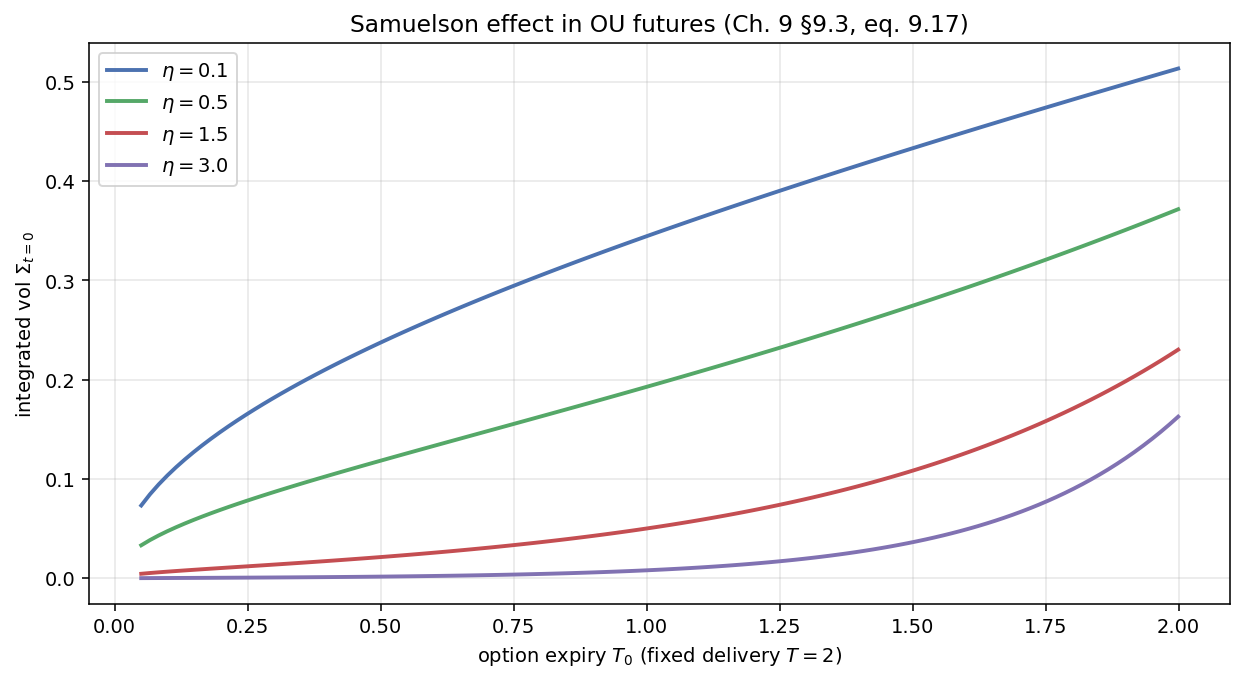
\includegraphics[keepaspectratio]{figures/ch08-samuelson-ou.png}}
\emph{Samuelson decay --- the vol loading \(\sigma e^{-\eta(T-t)}\)
drops with tenor, so far-dated contracts respond less to same-size
shocks than near contracts.}

\subsection{8.9.3 Terminal distribution}\label{terminal-distribution-1}

From (8.38),

\[
F_{T_0}(T) - F_t(T) \;=\; \int_t^{T_0} \sigma\,e^{-\eta(T - u)}\,\mathrm{d}\widehat{W}_u. \tag{8.39}
\]

The integrand is deterministic, so the right-hand side is Gaussian with
mean zero. By Itô's isometry, the variance is

\[
\Sigma_t^2 \;=\; \int_t^{T_0} \sigma^2\,e^{-2\eta(T - u)}\,\mathrm{d}u \;=\; \sigma^2\,\frac{e^{-2\eta(T - T_0)} - e^{-2\eta(T - t)}}{2\eta}. \tag{8.40}
\]

Hence

\[
F_{T_0}(T) - F_t(T) \;\sim_{\mathbb{Q}}\; \mathcal{N}(0, \Sigma_t^2), \tag{8.41}
\]

conditional on \(\mathcal{F}_t\).

\textbf{Reading (8.40).} Formula (8.40) is worth staring at. It encodes
the total variance accumulated by the futures between \(t\) (now) and
\(T_0\) (option expiry), given that delivery is at \(T\). There are
three dials:

\begin{itemize}
\tightlist
\item
  \(\sigma\) is the peak instantaneous vol, attained at delivery
  (\(T = u\));
\item
  \(\eta\) is the speed at which long-dated vols decay below that peak;
\item
  the \(T - t\) vs \(T - T_0\) spacing controls where on the decay curve
  we are integrating.
\end{itemize}

Two useful limits:

\begin{itemize}
\tightlist
\item
  \textbf{\(\eta \to 0\).} Expanding the exponentials,
  \(\Sigma_t^2 \to \sigma^2\,(T_0
  - t)\) --- ordinary Brownian motion with constant vol.~The Samuelson
  decay vanishes.
\item
  \textbf{\(\eta \to \infty\).} The exponents push the integrand to
  essentially zero everywhere except in a tiny sliver just before \(T\),
  and \(\Sigma_t^2
  \to 0\): long-dated futures with infinite decay are stationary and
  have no vol.
\end{itemize}

Real markets sit in between, with \(\eta\) estimated in the range
\(0.3\) to \(2.0\) per year for many commodities and interest rates.

\subsection{8.9.4 Pricing the binary}\label{pricing-the-binary}

For the binary call \(\varphi(F) = \mathbf{1}_{\{F > K\}}\) at option
expiry \(T_0\), with \(r = 0\):

\[
h(t, F) \;=\; \mathbb{Q}_{t, F}(F_{T_0}(T) > K) \;=\; \mathbb{Q}(F_{T_0} - F_t > K - F_t), \tag{8.42}
\]

and writing \(F_{T_0} - F_t = \Sigma_t\,Z\) with
\(Z \sim \mathcal{N}(0, 1)\),

\[
h(t, F) \;=\; \mathbb{Q}\!\left(Z > \frac{K - F}{\Sigma_t}\right) \;=\; \Phi\!\left(\frac{F - K}{\Sigma_t}\right), \tag{8.43}
\]

with \(\Sigma_t\) defined in (8.40).

\textbf{Structural similarity.} Formula (8.43) has the same structural
shape as the Bachelier binary formula (8.36): both are \(\Phi\) of a
\((F - K)/\Sigma\) \(z\)-score. The Samuelson structure is entirely
packaged into the single number \(\Sigma_t\). This single-number
compression is a feature of the arithmetic-Brownian world: no matter how
baroque the vol surface of the futures, as long as the SDE is driftless
with a deterministic (possibly time-dependent) vol, the terminal
distribution is normal with variance equal to the integrated
instantaneous variance, and any digital-style payoff prices off \(\Phi\)
of a single \(z\)-score.

\subsection{8.9.5 Practical implications and HJM
pointer}\label{practical-implications-and-hjm-pointer}

The variance \(\Sigma_t^2\) shrinks as \(T - T_0\) grows, so options on
long-dated futures are dramatically cheaper than those on near-dated
ones at otherwise similar parameters. Numerical case: \(\sigma = 0.40\),
\(\eta =
1.0\), \(T = 2\), \(T_0 = 0.25\), \(F_0 = 50\), \(K = 55\) gives
\(\Sigma_0 \approx
0.0309\) --- about a sixth of the flat-vol Bachelier
\(\sigma\sqrt{T_0} = 0.20\). The OU futures of (8.38) is the
single-factor exponentially-decaying-vol case of the
Heath--Jarrow--Morton (HJM) framework; multi-factor HJM models of the
\emph{entire} forward curve are standard in commodity and fixed-income
practice (see Chapter 13 multi-factor short-rate and Chapter 14 LIBOR
market models).

\begin{center}\rule{0.5\linewidth}{0.5pt}\end{center}

\section{8.10 Margrabe Exchange Option --- A Numeraire Change Tour de
Force}\label{margrabe-exchange-option-a-numeraire-change-tour-de-force}

The Margrabe exchange option is the cleanest testbed for Ch. 5's
numeraire-change machinery. A frontal 2-D PDE is painful; a numeraire
change reduces it to a 1-D Black--Scholes put with no interest-rate
discount visible. Principle: \emph{if the payoff has a natural unit,
price in that unit}.

\subsection{8.10.1 Setup}\label{setup-2}

Suppose there are two traded assets \(A\) and \(B\) with dynamics under
the physical measure

\[
\frac{\mathrm{d}A_t}{A_t} \;=\; \mu^A\,\mathrm{d}t \;+\; \sigma^A\,\mathrm{d}W_t, \qquad
\frac{\mathrm{d}B_t}{B_t} \;=\; \mu^B\,\mathrm{d}t \;+\; \sigma^B\,\mathrm{d}W_t \qquad (\mathbb{P}), \tag{8.44}
\]

driven (for the moment) by the same scalar Brownian \(W\). The general
correlated case is handled by (8.55) below. We value the \emph{Margrabe
exchange option} paying

\[
\mathcal{C} \;=\; \max(A_T - B_T,\, 0) \tag{8.45}
\]

A call on \(A\) struck at \(B\) --- or equivalently a put on \(B\)
struck at \(A\). The strike is random, moving with the underlying.
Denominate in units of \(A\) and the strike becomes the constant 1; the
problem collapses to a put on \(B/A\) struck at 1.

\pandocbounded{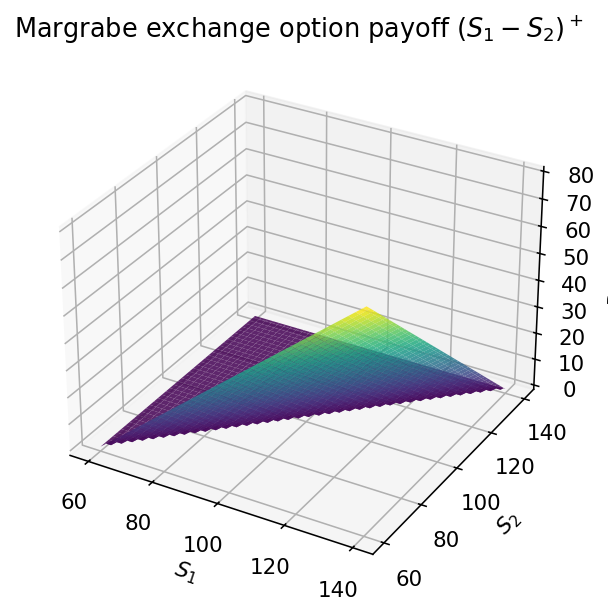
\includegraphics[keepaspectratio]{figures/ch08-margrabe.png}}
\emph{Margrabe exchange option payoff surface \(\max(A_T - B_T, 0)\)
across \((A_T, B_T)\).}

\subsection{\texorpdfstring{8.10.2 Step 1 --- Risk-neutral pricing under
\(\mathbb{Q}\)}{8.10.2 Step 1 --- Risk-neutral pricing under \textbackslash mathbb\{Q\}}}\label{step-1-risk-neutral-pricing-under-mathbbq}

First, change measure from \(\mathbb{P}\) to the bank-account measure
\(\mathbb{Q}\) so that both assets drift at the risk-free rate \(r\):

\[
\frac{\mathrm{d}A_t}{A_t} \;=\; r\,\mathrm{d}t \;+\; \sigma^A\,\mathrm{d}W_t^{\mathbb{Q}}, \qquad
\frac{\mathrm{d}B_t}{B_t} \;=\; r\,\mathrm{d}t \;+\; \sigma^B\,\mathrm{d}W_t^{\mathbb{Q}}. \tag{8.46}
\]

(Girsanov's theorem from Chapter 5 guarantees such a measure exists,
with drift shifts \(\lambda^A = (\mu^A - r)/\sigma^A\) and
\(\lambda^B = (\mu^B -
r)/\sigma^B\). When the same \(W\) drives both, consistency requires
\(\lambda^A = \lambda^B\) --- the market-price-of-risk condition of
Chapter 6.)

The risk-neutral price is

\[
f(t, A, B) \;=\; \mathbb{E}^{\mathbb{Q}}_{t, A, B}\!\left[\,(A_T - B_T)_+\,e^{-r(T - t)}\,\right]. \tag{8.47}
\]

Trying to evaluate (8.47) directly requires a two-dimensional log-normal
integral in \((A_T, B_T)\) --- feasible but not elegant.

\subsection{\texorpdfstring{8.10.3 Step 2 --- Change numeraire to
\(A\)}{8.10.3 Step 2 --- Change numeraire to A}}\label{step-2-change-numeraire-to-a}

Divide both sides of (8.47) by \(A_t\). By the general numeraire-pricing
identity of Chapter 5,

\[
\frac{f(t, A, B)}{A_t} \;=\; \mathbb{E}^{\mathbb{Q}^A}_{t, A, B}\!\left[\,\frac{(A_T - B_T)_+}{A_T}\,\right] \;=\; \mathbb{E}^{\mathbb{Q}^A}_{t, A, B}\!\left[\,\Bigl(1 - \tfrac{B_T}{A_T}\Bigr)_+\,\right], \tag{8.48}
\]

where \(\mathbb{Q}^A\) is the measure with numeraire \(A\) --- under
which every traded asset divided by \(A\) is a martingale. The
Radon--Nikodym density is
\(\mathrm{d}\mathbb{Q}^A / \mathrm{d}\mathbb{Q} = (A_T/A_0)/(M_T/M_0)\),
as derived in Chapter 5.

Dividing by \(A_t\) reinterprets ``price'' as ``shares of \(A\).'' The
price-in-\(A\) is a \(\mathbb{Q}^A\)-martingale, killing the discount
entirely. What remains is a put on \(X_T = B_T/A_T\) struck at 1 --- a
one-dimensional problem. Define

\[
X_t \;\equiv\; \frac{B_t}{A_t}, \tag{8.49}
\]

which, being the price of the traded asset \(B\) expressed in numeraire
\(A\), is a \(\mathbb{Q}^A\)-martingale.

\subsection{\texorpdfstring{8.10.4 Step 3 --- Dynamics of \(X_t\) under
\(\mathbb{Q}^A\)}{8.10.4 Step 3 --- Dynamics of X\_t under \textbackslash mathbb\{Q\}\^{}A}}\label{step-3-dynamics-of-x_t-under-mathbbqa}

To evaluate (8.48) we need the SDE for \(X_t\) under \(\mathbb{Q}^A\).
The Girsanov shift from \(\mathbb{Q}\) to \(\mathbb{Q}^A\), derived in
Chapter 5, is

\[
\mathrm{d}W_t^{\mathbb{Q}} \;=\; \sigma^A\,\mathrm{d}t \;+\; \mathrm{d}W_t^A, \tag{8.50}
\]

i.e.~the \(\mathbb{Q}\)-Brownian picks up a drift equal to the
volatility loading of the numeraire \(A\) when viewed under
\(\mathbb{Q}^A\).

Compute \(\mathrm{d}(1/A_t)\) via Itô on \(f(A) = 1/A\), with
\(f' = -1/A^2\), \(f'' = 2/A^3\):

\[
\mathrm{d}\!\left(\frac{1}{A_t}\right) \;=\; -\frac{\mathrm{d}A_t}{A_t^2} \;+\; \tfrac12 \cdot \frac{2}{A_t^3}\,(\sigma^A A_t)^2\,\mathrm{d}t \;=\; \frac{1}{A_t}\bigl[((\sigma^A)^2 - r)\,\mathrm{d}t \;-\; \sigma^A\,\mathrm{d}W_t^{\mathbb{Q}}\bigr]. \tag{8.51}
\]

Then, using the Itô product rule on \(X_t = B_t \cdot (1/A_t)\) with
covariation
\(\mathrm{d}[B, 1/A]_t = -(B_t/A_t)\,\sigma^A \sigma^B\,\mathrm{d}t\),

\[
\mathrm{d}\!\left(\frac{B_t}{A_t}\right) \;=\; \frac{B_t}{A_t}\bigl(r\,\mathrm{d}t + \sigma^B\,\mathrm{d}W_t^{\mathbb{Q}}\bigr) \;+\; \frac{B_t}{A_t}\bigl[((\sigma^A)^2 - r)\,\mathrm{d}t - \sigma^A\,\mathrm{d}W_t^{\mathbb{Q}}\bigr] \;-\; \frac{B_t}{A_t}\,\sigma^A \sigma^B\,\mathrm{d}t. \tag{8.52}
\]

Collecting \(\mathrm{d}t\) and \(\mathrm{d}W_t^{\mathbb{Q}}\) terms,

\[
\mathrm{d}\!\left(\frac{B_t}{A_t}\right) \;=\; \frac{B_t}{A_t}\Bigl\{\bigl[(\sigma^A)^2 - \sigma^A \sigma^B\bigr]\,\mathrm{d}t \;+\; (\sigma^B - \sigma^A)\,\mathrm{d}W_t^{\mathbb{Q}}\Bigr\}. \tag{8.53}
\]

Now substitute (8.50)
\(\mathrm{d}W_t^{\mathbb{Q}} = \sigma^A\,\mathrm{d}t +
\mathrm{d}W_t^A\):

\[
\mathrm{d}\!\left(\frac{B_t}{A_t}\right) \;=\; \frac{B_t}{A_t}\Bigl\{\underbrace{\bigl[(\sigma^A)^2 - \sigma^A \sigma^B + (\sigma^B - \sigma^A)\sigma^A\bigr]}_{\;=\; 0}\,\mathrm{d}t \;+\; (\sigma^B - \sigma^A)\,\mathrm{d}W_t^A\Bigr\}, \tag{8.54}
\]

confirming that \(X_t = B_t/A_t\) is a \(\mathbb{Q}^A\)-martingale, and

\[
\boxed{\;\frac{\mathrm{d}X_t}{X_t} \;=\; (\sigma^B - \sigma^A)\,\mathrm{d}W_t^A.\;} \tag{8.55}
\]

\(X\) is GBM with zero drift (forced by the numeraire property) and
\emph{relative} vol \(\sigma^B - \sigma^A\). When \(A\) and \(B\) have
the same vol and Brownian, the ratio is deterministic and the option
degenerates.

\subsection{8.10.5 Correlated case}\label{correlated-case}

In the general correlated case with two distinct Brownians
\(W^{(1)}, W^{(2)}\) of correlation \(\rho\),

\[
\frac{\mathrm{d}A_t}{A_t} \;=\; r\,\mathrm{d}t + \sigma^A\,\mathrm{d}W^{(1)}_t, \qquad
\frac{\mathrm{d}B_t}{B_t} \;=\; r\,\mathrm{d}t + \sigma^B\,\mathrm{d}W^{(2)}_t, \qquad \mathrm{d}\langle W^{(1)}, W^{(2)}\rangle_t = \rho\,\mathrm{d}t,
\]

the same Itô calculation yields
\(\mathrm{d}X_t / X_t = \hat{\sigma}\,\mathrm{d}W^A_t\) with

\[
\boxed{\;\hat{\sigma}^2 \;=\; (\sigma^A)^2 \;-\; 2\rho\,\sigma^A \sigma^B \;+\; (\sigma^B)^2.\;} \tag{8.56}
\]

The scalar-BM result (8.55) is the special case \(\rho = +1\) with both
assets driven by the \emph{same} \(W\), which collapses (8.56) to
\(\hat{\sigma}^2 =
(\sigma^B - \sigma^A)^2\) and hence
\(\hat{\sigma} = |\sigma^B - \sigma^A|\).

\textbf{Reading (8.56).} The only inter-asset interaction that matters
is correlation --- not individual drifts or levels. \(\rho \to +1\):
\(\hat{\sigma}^2 \to (\sigma^A - \sigma^B)^2\), lockstep assets cannot
diverge, option is cheap. \(\rho \to -1\):
\(\hat{\sigma}^2 \to (\sigma^A + \sigma^B)^2\), maximally divergent,
option is expensive. Correlation is the pricing input --- more than vol
--- which is why dispersion traders obsess over it.

\pandocbounded{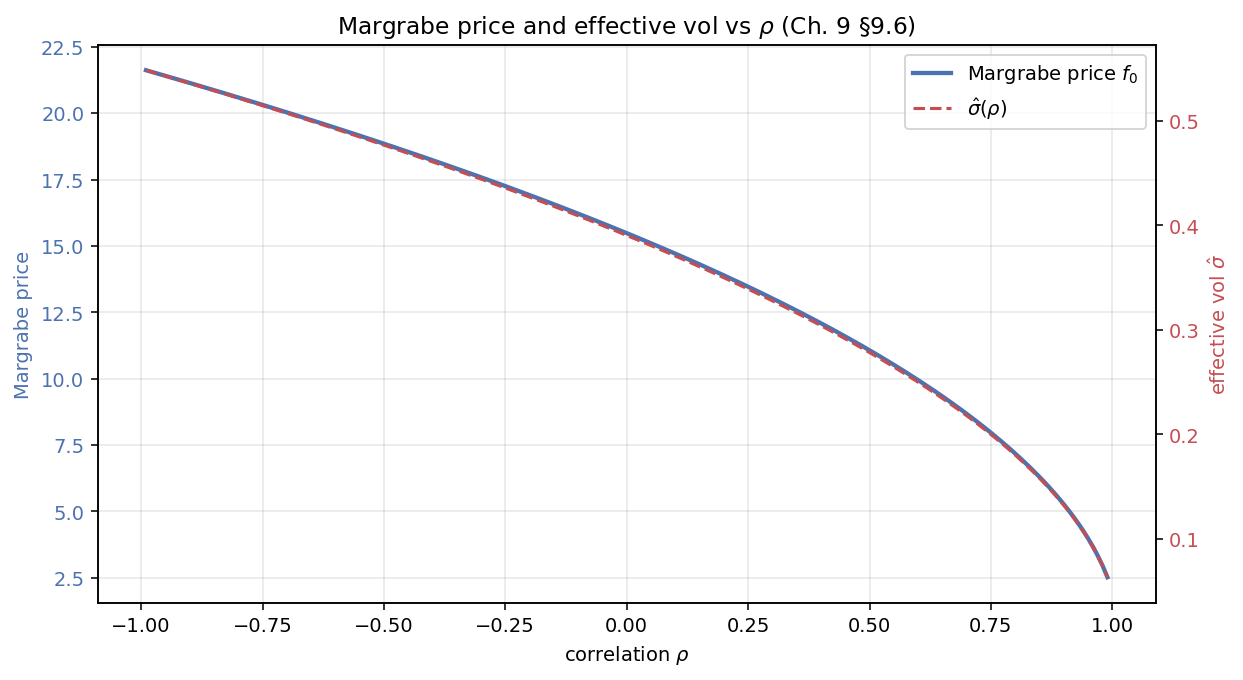
\includegraphics[keepaspectratio]{figures/ch08-margrabe-correlation.png}}
\emph{Margrabe price as a function of correlation \(\rho\) --- option
value increases monotonically as \(\rho\) decreases, since divergent
assets maximise the expected spread.}

\subsection{8.10.6 Step 4 --- The Margrabe
formula}\label{step-4-the-margrabe-formula}

Since \(X_t\) is a geometric Brownian motion under \(\mathbb{Q}^A\) with
volatility \(\hat{\sigma}\) and \emph{no drift}, the inner expectation
in (8.48) is a Black--Scholes put on \(X\) struck at 1 with \(r = 0\)
(no discount under the martingale measure):

\[
\frac{f_t}{A_t} \;=\; \Phi(d_+) \;-\; \frac{B_t}{A_t}\,\Phi(d_-), \qquad d_\pm \;=\; \frac{-\ln(B_t/A_t) \pm \tfrac12 \hat{\sigma}^2 (T - t)}{\hat{\sigma}\,\sqrt{T - t}}. \tag{8.57}
\]

Rearranging into the familiar Margrabe form,

\[
\boxed{\;f_t \;=\; A_t\,\Phi(d_1) \;-\; B_t\,\Phi(d_2),\;} \qquad d_1 \;=\; \frac{\ln(A_t/B_t) + \tfrac12 \hat{\sigma}^2 (T - t)}{\hat{\sigma}\,\sqrt{T - t}}, \quad d_2 \;=\; d_1 - \hat{\sigma}\,\sqrt{T - t}. \tag{8.58}
\]

No discounting appears because we priced under \(\mathbb{Q}^A\) and the
payoff is denominated in units of \(A\); the numeraire absorbs the
interest rate.

\subsection{8.10.7 Reading (8.58)}\label{reading-8.58}

The formula is BS in disguise: \(S \to A\), \(K e^{-rT} \to B\),
\(\sigma \to
\hat\sigma\). Margrabe sees only the \emph{ratio} \(A/B\), not absolute
levels; ATM is \(A_t = B_t\). Higher \(\rho\) shrinks \(\hat\sigma\), so
the option is cheapest when the two underlyings are clones; the
degenerate limit \(\rho = 1, \sigma^A = \sigma^B\) gives
\(\hat\sigma = 0\) and the option collapses to its intrinsic
\(\max(A_t - B_t, 0)\).

\subsection{8.10.9 Worked numerical
example}\label{worked-numerical-example}

Take \(A_0 = B_0 = 100\) (ATM), \(\sigma^A = 0.25\),
\(\sigma^B = 0.30\), \(\rho
= 0.6\), \(T = 1\) year, \(r = 3\%\). Then

\[
\hat{\sigma}^2 \;=\; 0.25^2 - 2 \cdot 0.6 \cdot 0.25 \cdot 0.30 + 0.30^2 \;=\; 0.0625 - 0.09 + 0.09 \;=\; 0.0625,
\]

so \(\hat{\sigma} = 0.25\). \(d_1 = 0.125\), \(d_2 = -0.125\),
\(\Phi \approx 0.5497/0.4503\):

\[
f_0 \;=\; 100 \cdot 0.5497 \;-\; 100 \cdot 0.4503 \;=\; 9.94.
\]

No discount factor --- the numeraire-change magic of (8.58). Now flip
\(\rho \to -0.6\):

\[
\hat{\sigma}^2 \;=\; 0.0625 + 0.09 + 0.09 \;=\; 0.2425, \qquad \hat{\sigma} \;\approx\; 0.4924.
\]

Spread vol nearly doubles, price rises to \(\approx 19.5\) --- flipping
\(\rho\) from \(+0.6\) to \(-0.6\) doubles the fair price. This is the
relationship dispersion desks live by.

\subsection{8.10.10 Generalisations and
pitfalls}\label{generalisations-and-pitfalls}

Stochastic vol in either leg pushes (8.58) into characteristic-function
/ MC territory; best-of \(\max(A_T, B_T, C_T)\) has no closed-form
analogue (Stulz 1982, Johnson 1987); dividend yields adjust the drifts
but leave the formula intact. \emph{Pitfall:} the \(\sigma^A, \sigma^B\)
in (8.56) must be loadings on the \emph{same} Brownian components; for
two independent Brownians (\(\rho = 0\)) the spread vol reduces to the
Pythagorean sum \(\hat\sigma =
\sqrt{(\sigma^A)^2 + (\sigma^B)^2}\).

\begin{center}\rule{0.5\linewidth}{0.5pt}\end{center}

\section{8.11 Futures vs Forward --- Convexity Adjustment Under
Stochastic
Rates}\label{futures-vs-forward-convexity-adjustment-under-stochastic-rates}

Under stochastic rates, futures and forwards differ by a convexity
adjustment whose sign tracks \(\mathrm{Cov}^{\mathbb{Q}}(r_t, S_t)\).

\subsection{8.11.1 The intuition}\label{the-intuition}

Bob is long a futures, Alice is long a forward (same \(T\), same final
exposure). Bob receives daily MTM cash; Alice does not. With
\(\mathrm{Cov}(r, S) > 0\), on Bob's up-days rates are high (reinvest at
high rate); on his down-days rates are low (finance at low rate). Bob
wins on the timing asymmetry, so the fair futures price must sit
\emph{above} the forward at inception. Negative correlation flips it.
Deterministic rates or zero correlation: the two coincide.

\subsection{8.11.2 The formula}\label{the-formula}

Under \(\mathbb{Q}\), \(F^{\text{fut}}\) is a martingale (§8.3); under
\(\mathbb{Q}^T\), \(F^{\text{fwd}}\) is. Conditional expectations:

\[
F^{\text{fut}}(t, T) \;=\; \mathbb{E}^{\mathbb{Q}}_t[S_T], \qquad
F^{\text{fwd}}(t, T) \;=\; \mathbb{E}^{\mathbb{Q}^T}_t[S_T] \;=\; \frac{\mathbb{E}^{\mathbb{Q}}_t\!\left[S_T\,e^{-\int_t^T r_u\,\mathrm{d}u}\right]}{P(t, T)}. \tag{8.59}
\]

Their difference is the convexity adjustment. By the identity
\(\mathrm{Cov}(X, Y) = \mathbb{E}[XY] - \mathbb{E}[X]\mathbb{E}[Y]\)
applied to the inner expectation, one obtains

\[
F^{\text{fut}}(t, T) \;-\; F^{\text{fwd}}(t, T) \;=\; \frac{1}{P(t, T)}\,\mathrm{Cov}^{\mathbb{Q}}_t\!\left(S_T,\,1 - e^{-\int_t^T r_u\,\mathrm{d}u}\right), \tag{8.60}
\]

which to leading order in the covariance is approximately

\[
F^{\text{fut}}(t, T) \;-\; F^{\text{fwd}}(t, T) \;\approx\; \int_t^T\!\!\int_t^T \mathrm{Cov}^{\mathbb{Q}}_t\bigl(\mathrm{d}\ln S_u,\,r_v\,\mathrm{d}v\bigr). \tag{8.61}
\]

\subsection{8.11.3 The sign rule}\label{the-sign-rule}

{\def\LTcaptype{none} % do not increment counter
\begin{longtable}[]{@{}
  >{\raggedright\arraybackslash}p{(\linewidth - 2\tabcolsep) * \real{0.5000}}
  >{\raggedright\arraybackslash}p{(\linewidth - 2\tabcolsep) * \real{0.5000}}@{}}
\toprule\noalign{}
\begin{minipage}[b]{\linewidth}\raggedright
Regime
\end{minipage} & \begin{minipage}[b]{\linewidth}\raggedright
Relation
\end{minipage} \\
\midrule\noalign{}
\endhead
\bottomrule\noalign{}
\endlastfoot
\(r\) deterministic &
\(F^{\text{fut}}(t, T) = F^{\text{fwd}}(t, T) = S_t / P(t, T)\) \\
\(r\) stochastic,
\(\mathrm{Cov}^{\mathbb{Q}}(r_t, F^{\text{fut}}_t) = 0\) &
\(F^{\text{fut}} = F^{\text{fwd}}\) \\
\(r\) stochastic, positive correlation &
\(F^{\text{fut}} > F^{\text{fwd}}\) \\
\(r\) stochastic, negative correlation &
\(F^{\text{fut}} < F^{\text{fwd}}\) \\
\end{longtable}
}

The two measures --- bank-account and \(T\)-forward --- coincide iff
\(P(t, T)\) is deterministic. When they coincide, so do the
expectations.

\pandocbounded{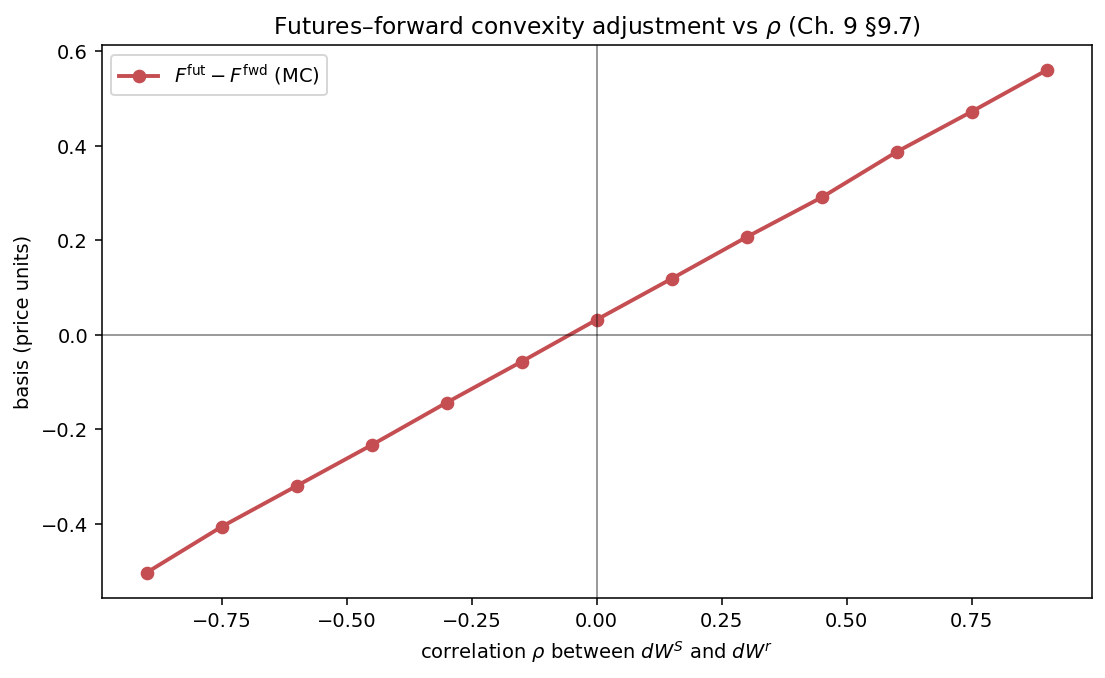
\includegraphics[keepaspectratio]{figures/ch08-fut-fwd-basis.png}}
\emph{Futures-forward basis under stochastic rates --- positive
\(r\)--\(S\) correlation pushes the basis positive, negative correlation
pushes it negative. The magnitude is controlled by rate volatility and
the tenor.}

\subsection{8.11.4 Magnitudes in practice}\label{magnitudes-in-practice}

How big is the convexity adjustment? A rough rule of thumb:

\begin{itemize}
\tightlist
\item
  \textbf{Short-dated eurodollar / SOFR futures.} Here the underlying
  rate and the reinvestment rate are both tied to the same short-rate
  curve, so \(\rho \approx 1\) and the correlation effect is maximal.
  The adjustment can reach several basis points and is routinely quoted
  and hedged by rates desks. Dedicated convexity-adjustment calculators
  are standard in rates-trading software.
\item
  \textbf{Long-dated equity index futures.} Correlation between equity
  returns and rates is modest, rate vols are low, and the adjustment is
  typically small (a few basis points on a multi-year contract). Still,
  for institutional hedgers running multi-billion-dollar exposures, a
  few basis points can matter.
\item
  \textbf{FX futures.} Non-trivial because of the ``quanto'' correlation
  between the FX rate and the domestic short rate. The formula (8.61) is
  still the starting point, but the practitioner's job is to specify a
  model (typically Hull--White for the short rate, log-normal for FX,
  with a correlation \(\rho\) between them) and evaluate the double
  integral analytically.
\end{itemize}

\subsection{8.11.5 The deeper reading}\label{the-deeper-reading}

The convexity adjustment is a \emph{measure-change effect}:
\(F^{\text{fut}}\) and \(F^{\text{fwd}}\) are both martingales but under
different measures (bank account vs \(T\)-forward), and those measures
diverge whenever rates are stochastic. The same structural pattern
reappears for CMS convexity (Chapter 13) and quanto adjustments under
FX.

\subsection{8.11.6 A Hull--White closed-form
approximation}\label{a-hullwhite-closed-form-approximation}

Writing down a concrete convexity-adjustment number requires a model for
both \(S\) and \(r\). The most common textbook choice is to take \(S\)
log-normal and \(r\) Hull--White (Chapter 12), with a constant
correlation \(\rho\) between the Brownians. Under that model, Hull
(2018) gives the approximation

\[
\ln F^{\text{fut}}(t, T) - \ln F^{\text{fwd}}(t, T) \;\approx\; \rho\,\sigma_S\,\sigma_r\,\frac{(T - t)^2}{2},
\]

where \(\sigma_S\) is the spot volatility and \(\sigma_r\) is the
short-rate vol.~The quadratic-in-tenor scaling is characteristic of
convexity adjustments: over short tenors the effect is negligible, but
it grows quickly with maturity. For eurodollar/SOFR futures with
\(\sigma_r \approx
0.01\) (1\% absolute rate vol), \(\sigma_S \approx 0.0025\) (own-vol for
a short rate), \(\rho \approx 1\), and \(T - t = 5\) years, the
adjustment is roughly \(1 \cdot 0.01 \cdot 0.0025 \cdot 12.5 = 0.0003\)
or 3 basis points --- a number that matches practitioner quotations for
multi-year eurodollar convexity adjustments.

\subsection{8.11.7 Hedging implications}\label{hedging-implications}

Dealers running futures-vs-forward basis books mark to the evolving
convexity adjustment daily; the basis's sensitivity to rate vol is the
\emph{vega of the convexity adjustment}, and is a standard rate-vol-desk
diagnostic.

\begin{center}\rule{0.5\linewidth}{0.5pt}\end{center}

\section{8.12 Key Takeaways}\label{key-takeaways-7}

\begin{enumerate}
\def\labelenumi{\arabic{enumi}.}
\item
  \textbf{Forward price.} The fair forward strike
  \(F^{\text{fwd}}_t(T) = S_t /
  P(t, T)\) is pinned by cash-and-carry no-arbitrage, independent of
  volatility or any statistical properties of \(S\). Under constant
  rates this reduces to \(S_t\,e^{r(T - t)}\); with a dividend yield, to
  \(S_t\,e^{(r - \delta)(T - t)}\).
\item
  \textbf{Forwards vs futures.} Forwards settle at maturity; futures
  settle daily. The futures position is zero-valued at every instant by
  design (daily MTM absorbs every infinitesimal gain/loss immediately),
  while the forward's value drifts with the spot until maturity. This
  zero-value feature is why the futures price is a
  \(\mathbb{Q}\)-martingale and why the Black PDE has no
  first-derivative drift term.
\item
  \textbf{Three drifts under \(\mathbb{Q}\).}

  \begin{itemize}
  \tightlist
  \item
    Traded asset: drift \(r\,X_t\).
  \item
    Traded asset with yield \(\delta\): drift \((r - \delta)\,X_t\).
  \item
    Futures quote: drift \(0\) (costless position).
  \end{itemize}
\item
  \textbf{Dynamics of \(F_t\) under \(\mathbb{Q}\).}
  \(\mathrm{d}F_t(T) = \sigma^F(t,
  F)\,\mathrm{d}\widehat{W}_t\) with no drift. Specific choices of
  \(\sigma^F\) yield GBM (constant relative vol, used in Black '76),
  Bachelier (constant absolute vol, used when \(F\) can go negative),
  and Samuelson/OU (time-decaying vol loading, used for commodity
  futures).
\item
  \textbf{Black PDE.} For an option \(g(t, F)\) on a futures with payoff
  \(\varphi(F_{T_0})\),

  \[
  \partial_t g \;+\; \tfrac12\,(\sigma^F)^2\,\partial_{FF} g \;=\; r\,g, \qquad g(T_0, F) = \varphi(F).
  \]

  The missing \(r\,F\,\partial_F g\) term is the signature of
  martingale-underlying pricing. The \(r\,g\) discount term remains
  because the option's dollar payoff still settles at \(T_0\).
\item
  \textbf{Feynman--Kac cross-check.} The Black PDE has the stochastic
  representation \(g(t, F) = \mathbb{E}^{\mathbb{Q}}[\,e^{-r(T_0 -
  t)}\,\varphi(F_{T_0})\,|\,F_t = F\,]\) with \(F_u\) satisfying the
  driftless SDE under \(\mathbb{Q}\).
\item
  \textbf{Black '76 closed form.} For log-normal futures with constant
  relative vol \(\sigma\) and a call payoff,

  \[
  g(t, F) \;=\; e^{-r(T_0 - t)}\,[F\,\Phi(d_+) \;-\; K\,\Phi(d_-)], \qquad d_\pm \;=\; \frac{\ln(F/K) \pm \tfrac12 \sigma^2 (T_0 - t)}{\sigma\,\sqrt{T_0 - t}}.
  \]

  Structurally, Black '76 is BS with \(S \to F\), \(r \to 0\) in
  \(d_\pm\), and an overall discount \(e^{-r(T_0 - t)}\).
\item
  \textbf{Bachelier binary.} Under
  \(\mathrm{d}F_t = \sigma\,\mathrm{d}\widehat{W}_t\), a digital call
  prices as \(\Phi((F - K)/(\sigma\,\sqrt{T_0 - t}))\). At the money
  (\(F = K\)), the price is exactly \(1/2\) --- a symmetry unique to the
  arithmetic model.
\item
  \textbf{Samuelson / OU futures.} Under
  \(\mathrm{d}F_t = \sigma\,e^{-\eta(T -
  t)}\,\mathrm{d}\widehat{W}_t\), terminal variance is
  \(\Sigma_t^2 = \sigma^2\,(e^{-2\eta(T - T_0)} - e^{-2\eta(T -
  t)})/(2\eta)\) and a digital call prices as
  \(\Phi((F - K)/\Sigma_t)\). Long-dated futures have smaller
  \(\Sigma_t\) than short-dated ones --- the Samuelson effect.
\item
  \textbf{Margrabe exchange option.} Under numeraire \(A\), the ratio
  \(X_t =
  B_t/A_t\) is a martingale with vol \(\hat{\sigma} =
  \sqrt{(\sigma^A)^2 - 2\rho\,\sigma^A\sigma^B + (\sigma^B)^2}\),
  yielding \(f_t = A_t\,\Phi(d_1) - B_t\,\Phi(d_2)\). No discount factor
  appears because the numeraire absorbs interest. Correlation \(\rho\),
  not individual drifts or levels, determines the option value.
\item
  \textbf{Futures vs forward convexity.} Under stochastic rates,
  \(F^{\text{fut}} - F^{\text{fwd}}\) is a covariance of \(S_T\) with
  the rate-path discount factor, proportional to
  \(\mathrm{Cov}^{\mathbb{Q}}(r,
  S)\) in the leading-order limit. Positive correlation pushes the
  futures price above the forward; negative correlation pushes it below.
  Under deterministic rates, the two prices coincide.
\item
  \textbf{Numeraire is the theme.} The futures price is natural under
  \(\mathbb{Q}\); the forward price is natural under \(\mathbb{Q}^T\);
  the Margrabe exchange option is natural under one of its own legs.
  Each ``naturalness'' is an invitation to change measure; accepting the
  invitation collapses the pricing problem, while refusing it forces one
  to grind through a PDE that did not need to be set up.
\end{enumerate}

\begin{center}\rule{0.5\linewidth}{0.5pt}\end{center}

\section{Appendix --- Reference
Formulas}\label{appendix-reference-formulas}

{\def\LTcaptype{none} % do not increment counter
\begin{longtable}[]{@{}
  >{\raggedright\arraybackslash}p{(\linewidth - 2\tabcolsep) * \real{0.5000}}
  >{\raggedright\arraybackslash}p{(\linewidth - 2\tabcolsep) * \real{0.5000}}@{}}
\toprule\noalign{}
\begin{minipage}[b]{\linewidth}\raggedright
Label
\end{minipage} & \begin{minipage}[b]{\linewidth}\raggedright
Formula
\end{minipage} \\
\midrule\noalign{}
\endhead
\bottomrule\noalign{}
\endlastfoot
(8.3) & \(F^{\text{fwd}}_t(T) = S_t\,e^{r(T - t)}\) (constant rates, no
dividend) \\
(8.4) & \(F^{\text{fwd}}_t(T) = S_t / P(t, T)\) (cash-and-carry, any
rates) \\
(8.8) & \(\mathbb{E}^{\mathbb{Q}}[F_t(T) \mid \mathcal{F}_s] = F_s(T)\)
(futures is a \(\mathbb{Q}\)-martingale) \\
(8.9) &
\(\mathrm{d}F_t(T) = \sigma^F(t, F_t(T))\,\mathrm{d}\widehat{W}_t\)
(general futures SDE under \(\mathbb{Q}\)) \\
(8.13) & \(\mathrm{d}F_t/F_t = \sigma\,\mathrm{d}\widehat{W}_t\)
(log-normal futures under \(\mathbb{Q}\)) \\
(8.21) & \(\alpha_t = \partial_F g(t, F_t)\) (futures-delta hedge) \\
(8.24) &
\(\partial_t g + \tfrac12(\sigma^F)^2\,\partial_{FF} g = r\,g\),
\(g(T_0, F) = \varphi(F)\) (Black PDE) \\
(8.26) &
\(g(t, F) = \mathbb{E}^{\mathbb{Q}}[\,e^{-r(T_0 - t)}\,\varphi(F_{T_0})\,\|\,F_t = F\,]\)
(Feynman--Kac) \\
(8.30) & \(g = e^{-r(T_0 - t)}[F\,\Phi(d_+) - K\,\Phi(d_-)]\) (Black '76
call) \\
(8.31) &
\(d_\pm = [\ln(F/K) \pm \tfrac12\sigma^2(T_0 - t)]/(\sigma\sqrt{T_0 - t})\) \\
(8.32) & \(\partial_F g = e^{-r(T_0 - t)}\,\Phi(d_+)\) (Black '76
delta) \\
(8.36) & Bachelier binary:
\(h(t, F) = \Phi((F - K)/(\sigma\,\sqrt{T_0 - t}))\) \\
(8.40) & Samuelson variance:
\(\Sigma_t^2 = \sigma^2\,(e^{-2\eta(T - T_0)} - e^{-2\eta(T - t)})/(2\eta)\) \\
(8.43) & OU binary: \(h(t, F) = \Phi((F - K)/\Sigma_t)\) \\
(8.55) & \(\mathrm{d}X_t/X_t = (\sigma^B - \sigma^A)\,\mathrm{d}W_t^A\)
(Margrabe ratio dynamics, scalar BM) \\
(8.56) &
\(\hat{\sigma}^2 = (\sigma^A)^2 - 2\rho\,\sigma^A\sigma^B + (\sigma^B)^2\)
(Margrabe spread vol) \\
(8.58) & Margrabe: \(f_t = A_t\,\Phi(d_1) - B_t\,\Phi(d_2)\) \\
(8.60) &
\(F^{\text{fut}} - F^{\text{fwd}} = \mathrm{Cov}^{\mathbb{Q}}_t(S_T,\,1 - e^{-\int r})\,/\,P(t, T)\) \\
(8.61) & Convexity
\(\approx \int_t^T\!\int_t^T \mathrm{Cov}^{\mathbb{Q}}_t(\mathrm{d}\ln S_u,\,r_v\,\mathrm{d}v)\) \\
\end{longtable}
}

\newpage

\chapter{Chapter 9 --- Monte Carlo, Path-Dependent, and Forward-Starting
Options}\label{chapter-9-monte-carlo-path-dependent-and-forward-starting-options}

The simulation counterpart to lattice pricing (Ch. 2) and PDE pricing
(Ch. 6). Closed forms cover only a short list of vanillas; everything
else --- Asians, lookbacks, cliquets, autocallables, baskets, stoch-vol,
jump-diffusions, local-vol surfaces --- needs numerical pricing. Monte
Carlo works in any dimension, handles any payoff, and parallelises
trivially; its only cost is statistical noise.

We motivate MC via the curse of dimensionality, build the GBM path
generator (exact, by the Ch. 6 Itô solution), and apply it to European
warm-ups, forward-starting cliquets (where iterated conditioning gives a
closed form), and barrier options (the prototypical path-dependent
payoff). Along the way we hit discretisation bias and the
Brownian-bridge correction. The chapter closes with antithetic and
control-variate variance reduction --- bridging to the Heston Monte
Carlo of Ch. 10.

Out of scope: stratified sampling, importance sampling, quasi-MC,
pathwise/LR Greek estimators, Longstaff--Schwartz for American exotics.
The focus is a working production-grade pricer for European and
path-dependent claims.

\begin{center}\rule{0.5\linewidth}{0.5pt}\end{center}

\section{9.1 Why Monte Carlo? Quadrature and the Curse of
Dimensionality}\label{why-monte-carlo-quadrature-and-the-curse-of-dimensionality}

The pricing integral
\(V_0 = e^{-rT}\,\mathbb{E}^{\mathbb{Q}}[\varphi(\cdot)]\) can be
evaluated by quadrature in low dimensions (\(O(h^p)\) error). In high
dimensions, quadrature dies: for a daily-monitored 1-year single-asset
option, \(d = 252\) and even \(N = 2\) points/dim gives
\(2^{252} \approx 10^{75}\) --- beyond any computer.

Monte Carlo's sample-mean error scales as \(M^{-1/2}\) \emph{regardless
of dimension}. Total cost \(O(Md)\) vs \(O(N^d)\) for quadrature.
Break-even is \(d \approx 4\)--\(6\); everything realistic lives above
that.

\begin{figure}
\centering
\pandocbounded{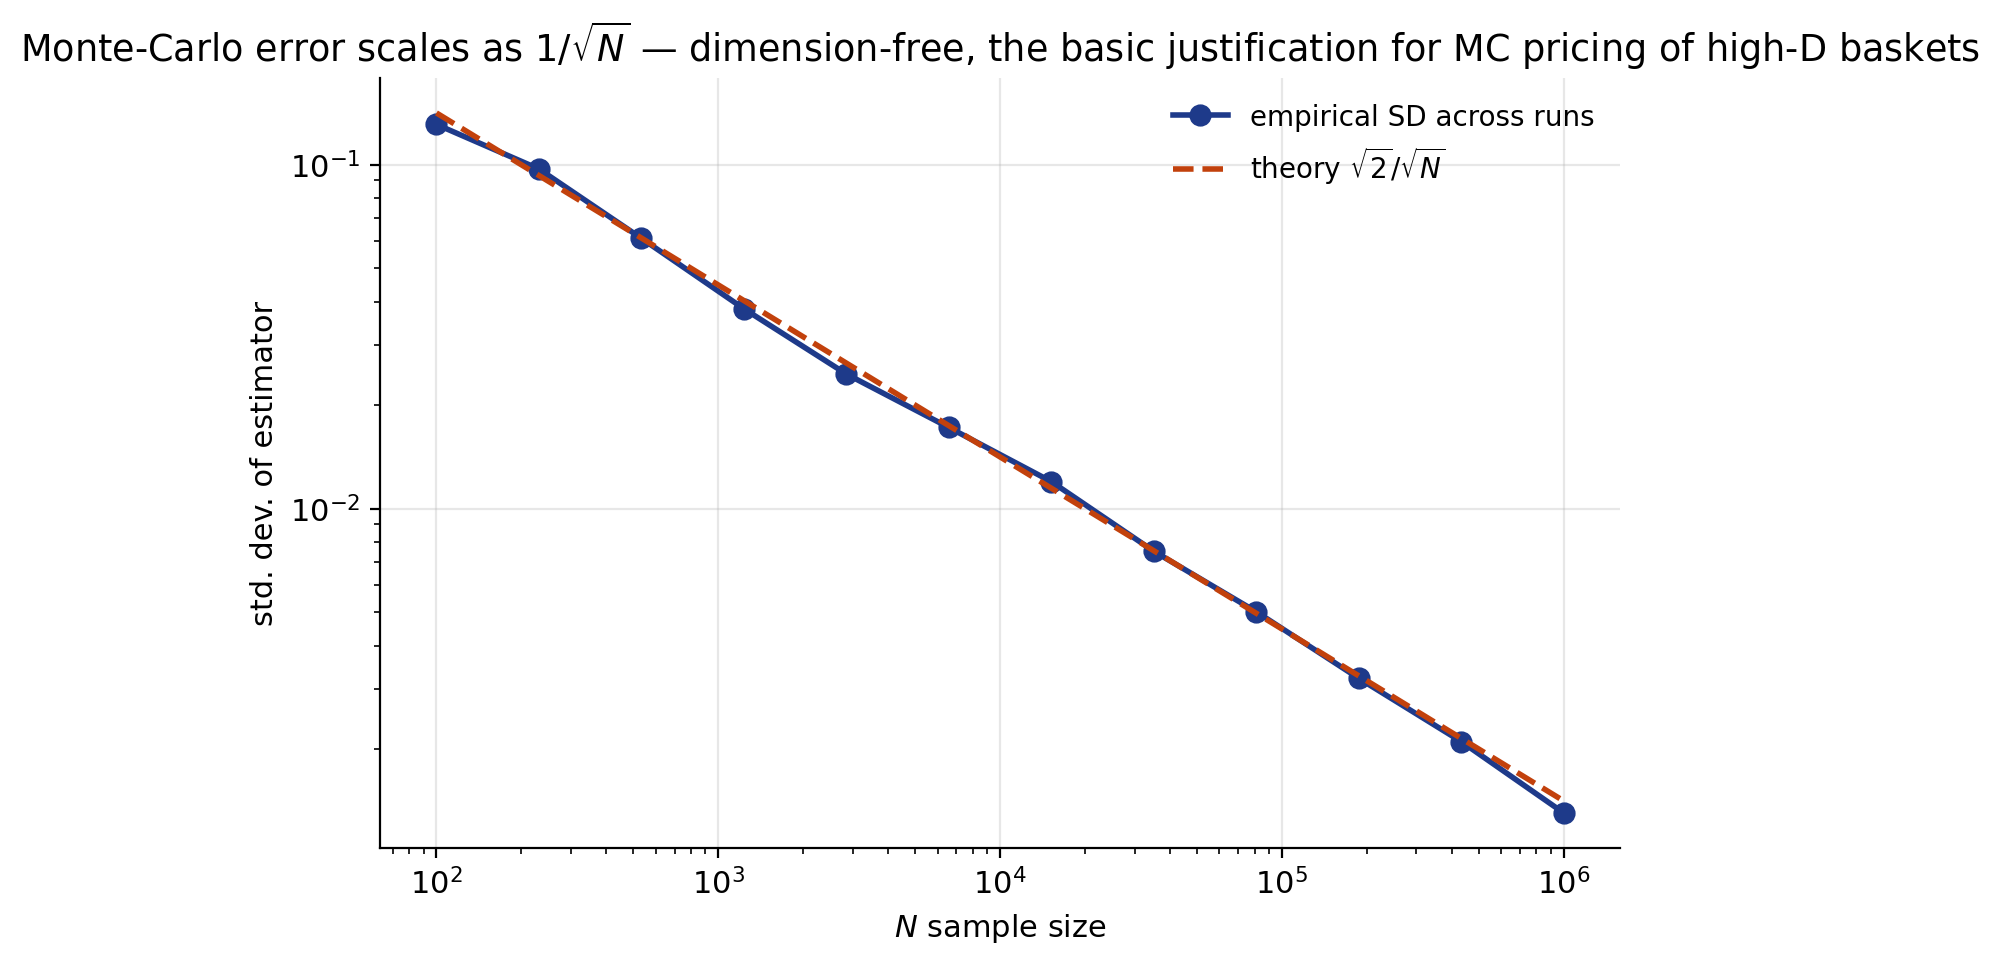
\includegraphics[keepaspectratio]{figures/ch09-sqrt-n-error.png}}
\caption{Empirical standard deviation of an MC estimator (here
\(\mathbb{E}[Z^2]=1\)) versus theoretical \(\sqrt{2}/\sqrt{N}\) across
four decades of sample size. The 1/\(\sqrt{N}\) slope is dimension-free
--- every desk's overnight risk-run reports confidence intervals that
respect this rate}
\end{figure}

The flip side: MC is statistical. Always report the standard error;
deterministic methods give bounds, MC gives confidence intervals.

A production pricer has four sub-problems:

\begin{enumerate}
\def\labelenumi{\arabic{enumi}.}
\tightlist
\item
  \textbf{Path generation under \(\mathbb{Q}\).} Given the chosen
  risk-neutral model --- GBM, Heston, local-vol, jump-diffusion, etc.
  --- produce paths whose law matches the specification. For GBM the
  exact lognormal increment of §9.4 gives a bias-free generator; for
  general SDEs one falls back on Euler--Maruyama or Milstein schemes
  with their associated discretisation biases.
\item
  \textbf{Variance reduction.} Reduce the sample variance so that fewer
  paths suffice to achieve a target confidence-interval width.
  Antithetic variates, control variates, stratified sampling, importance
  sampling, and quasi-random sequences each contribute.
\item
  \textbf{Path-dependent payoffs.} Many payoffs depend on the whole
  path: running maximum (lookback), running average (Asian),
  barrier-crossing indicator (knock-in/out), basket constraints.
  Efficient data structures and careful handling of between-grid events
  (Brownian-bridge correction for barriers) are central.
\item
  \textbf{Sensitivity estimation (Greeks).} Delta, gamma, vega, and
  other Greeks must come out of the same path sample, ideally with
  pathwise or likelihood-ratio estimators rather than finite-difference
  bump-and-reprice. We will touch on this briefly but not in depth.
\end{enumerate}

This chapter covers (1)--(3); Greek estimation (4) is a subdiscipline
left to Ch. 10 and the literature.

\begin{center}\rule{0.5\linewidth}{0.5pt}\end{center}

\section{9.2 The Strong Law of Large
Numbers}\label{the-strong-law-of-large-numbers}

Let \(X^{(1)}, \dots, X^{(M)}\) be i.i.d. copies of \(X\) with
\(\mathbb{E}|X| < \infty\). Then

\[
\lim_{M\to +\infty}\; \frac{X^{(1)} + X^{(2)} + \cdots + X^{(M)}}{M} \;=\; \mathbb{E}[X] \qquad \text{(strong law, a.s.).}
\tag{9.1}
\]

SLLN is the licence for MC pricing: enough i.i.d. payoff draws converge
a.s. to \(\mathbb{E}^{\mathbb{Q}}[\text{payoff}]\). Bounded payoffs
(puts capped at \(K\), digitals at 1) and polynomially-growing payoffs
on lognormal underlyings satisfy the integrability hypothesis trivially;
the pathological case is heavy-tailed (Cauchy-like) variables, where the
sample mean inherits the heavy tail and never converges.

\(L^2\) integrability gives the CLT:

\[
\sqrt{M}\,\bigl(\widehat{m}_M - \mathbb{E}[X]\bigr) \;\xrightarrow{d}\; \mathcal{N}\bigl(0,\;\mathbb{V}[X]\bigr),
\tag{9.2}
\]

--- the basis for the \(\widehat{m}_M \pm 1.96\,\widehat{\sigma}_{m_1}\)
95\% CI. Problem cases are reciprocals/roots of the underlying,
stoch-vol near the Feller boundary (Ch. 10), and unbounded-horizon
integrals.

\begin{center}\rule{0.5\linewidth}{0.5pt}\end{center}

\section{9.3 Sample Mean, Sample Variance, and the Monte-Carlo Standard
Error}\label{sample-mean-sample-variance-and-the-monte-carlo-standard-error}

We estimate \(m_1 := \mathbb{E}[X]\) by the finite sample

\[
\widehat{m}_1 \;=\; \frac{1}{M}\,\sum_{m=1}^{M}\, X^{(m)} \qquad \text{(sample mean).}
\tag{9.3}
\]

The sample mean is unbiased
(\(\mathbb{E}[\widehat{m}_1] = \mathbb{E}[X]\)) because expectation is
linear, and has variance

\[
\mathbb{V}[\widehat{m}_1] \;=\; \frac{1}{M^2}\sum_{m=1}^M \mathbb{V}[X^{(m)}] \;=\; \frac{\mathbb{V}[X]}{M},
\tag{9.4}
\]

using independence of the draws. The standard deviation of the sample
mean is therefore \(\sigma_{m_1} = \mathrm{sd}[X]/\sqrt{M}\). Since
\(\sigma_{m_1}\) depends on the unknown population variance, we estimate
it by the sample-variance-based standard error

\[
\widehat{\sigma}_{m_1} \;=\; \frac{1}{\sqrt{M}}\!\left(\,\frac{1}{M-1}\sum_{m=1}^{M}\!\left(X^{(m)} - \widehat{m}_1\right)^2\,\right)^{\!1/2}.
\tag{9.5}
\]

Two notes on (9.5): the inner bracket has Bessel's \(M-1\) divisor
(unbiased sample variance); the outer \(\sqrt{M}\) converts the sample
SD into the SD of the \emph{sample mean} --- easy to confuse.

\(M^{-1/2}\) convergence: halving the error bar costs \(4\times\) more
paths, three to four significant figures costs \(100\times\), four to
five \(10{,}000\times\). This is why variance reduction matters (§9.8).

\pandocbounded{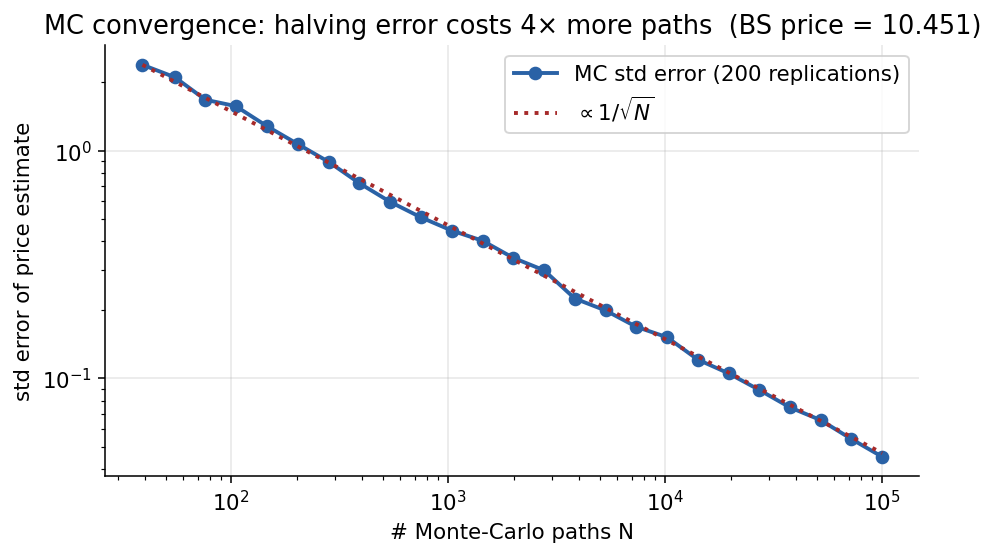
\includegraphics[keepaspectratio]{figures/ch10-mc-sqrt-rate.png}}
\emph{Empirical verification of the \(M^{-1/2}\) rate. The standard
deviation of the sample-mean estimator across 200 replications of an ATM
European-call MC price, plotted against path count \(M\) on log-log
axes, tracks the \(1/\sqrt{M}\) reference line over five decades.
Variance reduction (§9.8) changes the constant, not the slope.}

Concrete error budget. ATM 1-year call, \(S_0 = K = 100\), \(r = 5\%\),
\(\sigma = 20\%\). BS value \(\approx 10.45\), payoff std-dev
\(\approx 14\). With \(M = 10{,}000\), SE
\(= 14/\sqrt{10{,}000} = 0.14\), 95\% CI

\[
10.45 \pm 1.96\cdot 0.14 \;=\; [10.17,\; 10.73].
\]

For four-digit accuracy: \(M = (14/0.01)^2 \approx 2\)M paths. Doable in
seconds, but variance reduction earns its keep within a few million.

Trader ballparks:

\begin{itemize}
\tightlist
\item
  A standard-error budget of \(0.1\) on an option worth \(\sim 10\) is
  typically acceptable for a trading indication. That is
  \(M\sim 20{,}000\) paths for a vanilla European call at typical
  parameters.
\item
  A standard-error budget of \(0.01\) on a portfolio-level MC risk
  calculation is typically required for capital numbers. That is
  \(M\sim 2{,}000{,}000\) paths, an order of magnitude more effort.
\item
  Pathwise sensitivities (deltas, gammas) typically have standard
  deviations \(2\)--\(5\times\) higher than the price itself, so Greek
  estimation at fixed MC budget is \(4\times\)--\(25\times\) noisier
  than price estimation at the same budget. Practitioners either run
  more paths for Greeks or use variance-reduction techniques more
  aggressively on Greeks than on prices.
\end{itemize}

The SE is an estimate of an estimate; the Gaussian CI is asymptotic.
Small \(M\) → use Student-\(t\). Badly non-Gaussian payoffs (heavy-OTM,
rare-trigger barriers) → bootstrap rather than trust a symmetric CI.

\begin{center}\rule{0.5\linewidth}{0.5pt}\end{center}

\section{9.4 The Lognormal GBM Path
Generator}\label{the-lognormal-gbm-path-generator}

The path generator produces \(\{S_{t_n}\}\) from the \(\mathbb{Q}\)-law.
For GBM the generator is \emph{exact} at grid points (no discretisation
bias) because Ch. 6 solved the SDE in closed form.

\pandocbounded{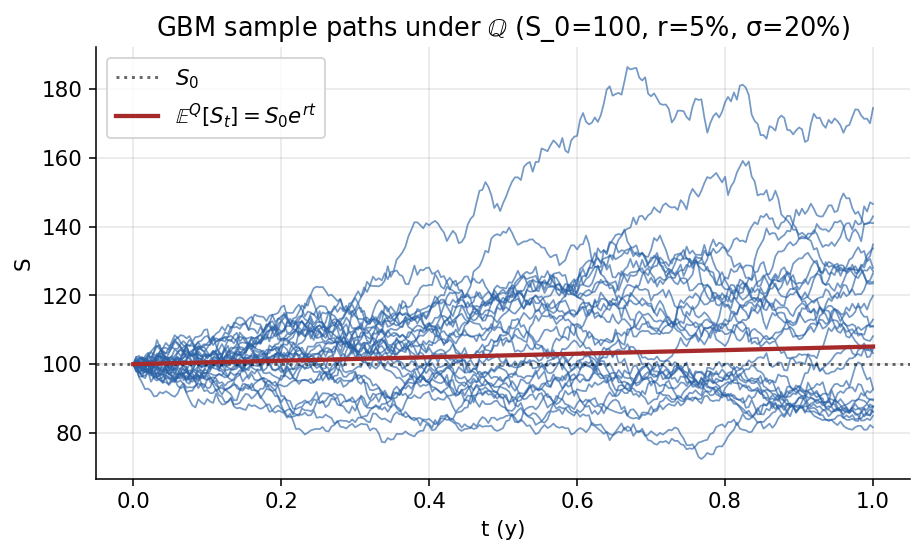
\includegraphics[keepaspectratio]{figures/ch10-gbm-paths.png}}
\emph{Thirty risk-neutral GBM paths for \(S_0 = 100\), \(r = 5\%\),
\(\sigma = 20\%\), \(T = 1\text{y}\). The red curve is
\(\mathbb{E}^{\mathbb{Q}}[S_t] = S_0 e^{rt}\), the risk-neutral expected
trajectory. Monte-Carlo pricing averages discounted payoffs over such
paths; each path contributes one term of the sample mean (9.3).}

\subsection{9.4.1 Exact lognormal
increment}\label{exact-lognormal-increment}

Under \(\mathbb{Q}\),

\[
\mathrm{d} S_t \;=\; r\,S_t\,\mathrm{d} t \;+\; \sigma\,S_t\,\mathrm{d} W_t^{\mathbb{Q}},
\tag{9.6}
\]

Itô on \(\ln S_t\):

\[
\mathrm{d}\ln S_t \;=\; \bigl(r - \tfrac{1}{2}\sigma^2\bigr)\,\mathrm{d} t \;+\; \sigma\,\mathrm{d} W_t^{\mathbb{Q}},
\tag{9.7}
\]

and integrating from \(t_{n-1}\) to \(t_n\),

\[
\ln S_{t_n} - \ln S_{t_{n-1}} \;=\; \bigl(r - \tfrac{1}{2}\sigma^2\bigr)\,\Delta t_n \;+\; \sigma\,\bigl(W^{\mathbb{Q}}_{t_n} - W^{\mathbb{Q}}_{t_{n-1}}\bigr),
\tag{9.8}
\]

with \(\Delta t_n := t_n - t_{n-1}\) and the Brownian increment exactly
Gaussian, independent of history. Exponentiating gives

\[
S_{t_n} \;=\; S_{t_{n-1}}\,\exp\!\Bigl\{\bigl(r - \tfrac{1}{2}\sigma^2\bigr)\,\Delta t_n \;+\; \sigma\sqrt{\Delta t_n}\,Z_n\Bigr\},
\qquad Z_1, Z_2, \dots \stackrel{\text{iid}}{\sim}_{\mathbb{Q}} \mathcal{N}(0,1).
\tag{9.9}
\]

The universal GBM generator. At grid points the law is exactly GBM ---
no discretisation bias. Between grid points the discrete path is a
log-linear interpolation; for payoffs that care (barriers, lookbacks) a
correction is needed (§9.7).

For non-GBM SDEs the increment is Gaussian only in the
\(\Delta t \to 0\) limit; Euler--Maruyama has weak error \(O(\Delta t)\)
and strong error \(O(\sqrt{\Delta t})\). Milstein upgrades strong to
\(O(\Delta t)\) via a second-order Itô correction. Strong order matters
for individual-realisation path-dependent payoffs.

\subsection{9.4.2 Monte-Carlo estimator for European
claims}\label{monte-carlo-estimator-for-european-claims}

For a European claim with payoff \(\varphi(S_T)\) the MC estimator is
the direct sample-average translation of the SLLN:

\[
\widehat{V}_0 \;=\; e^{-rT}\cdot \frac{1}{M}\sum_{m=1}^{M}\, \varphi\!\left(S_0\,e^{(r-\tfrac{1}{2}\sigma^2)T \;+\; \sigma\sqrt{T}\,Z^{(m)}}\right),
\qquad Z^{(m)} \stackrel{\text{iid}}{\sim}_{\mathbb{Q}} \mathcal{N}(0,1).
\tag{9.10}
\]

Only the terminal value \(S_T\) enters, so we do not even need a grid
--- a single Gaussian draw per path suffices. This is the
computationally cheapest non-trivial Monte-Carlo pricer and is useful
mainly as a sanity check against Black--Scholes and as a warm-up for the
path-dependent cases below.

\subsection{9.4.3 Euler--Maruyama and Milstein for non-GBM
SDEs}\label{eulermaruyama-and-milstein-for-non-gbm-sdes}

For Heston, local-vol, and jump-diffusion (Ch. 10) the exact lognormal
increment is unavailable. Euler--Maruyama freezes coefficients at the
left endpoint:

\[
X_{t_n} \;\approx\; X_{t_{n-1}} \;+\; \mu(X_{t_{n-1}})\,\Delta t_n \;+\; \sigma(X_{t_{n-1}})\sqrt{\Delta t_n}\,Z_n.
\]

Weak rate \(O(\Delta t)\), strong rate \(O(\sqrt{\Delta t})\). Milstein
adds a second-order Itô correction
\(\tfrac12 \sigma \sigma' \Delta t_n (Z_n^2 - 1)\) and upgrades the
strong rate to \(O(\Delta t)\). For constant diffusion (\(\sigma' = 0\))
both coincide.

The Heston variance process
\(\mathrm{d} v_t = \kappa(\theta - v_t)\mathrm{d}t + \xi\sqrt{v_t}\mathrm{d} W_t\)
has \(\sigma(v) = \xi\sqrt{v}\), non-differentiable at \(0\); naive
Euler produces negative variance. Standard fixes: full-truncation or
Andersen's QE scheme (Ch. 10). Whenever a closed-form exact simulator
exists (GBM, OU, CIR, Vasicek), prefer it over Euler.

\subsection{9.4.4 Additive log-space
simulation}\label{additive-log-space-simulation}

Simulating \(\ln S_{t_n}\) additively,

\[
\ln S_{t_n} \;=\; \ln S_{t_{n-1}} + (r - \tfrac{1}{2}\sigma^2)\,\Delta t_n \;+\; \sigma\sqrt{\Delta t_n}\,Z_n,
\tag{9.11}
\]

is algebraically identical but numerically more stable on
very-long-dated structures (no underflow at small \(S\)). Production
pricers typically work in log-space.

\subsection{9.4.5 Correlation of time-slices along a single
path}\label{correlation-of-time-slices-along-a-single-path}

For two times \(T_1 < T_2\) on the same GBM path,

\[
\mathbb{C}\!\left[S_{T_1}, S_{T_2}\right] \;=\; \operatorname{Cov}^{\mathbb{Q}}\!\left(S_{T_1}, S_{T_2}\right),
\qquad
\rho\!\left[S_{T_1}, S_{T_2}\right] \;=\; \frac{\mathbb{C}\!\left[S_{T_1}, S_{T_2}\right]}{\bigl(\mathbb{V}[S_{T_1}]\,\mathbb{V}[S_{T_2}]\bigr)^{1/2}}.
\tag{9.12}
\]

\(S_{T_2} = S_{T_1} \exp\{(r - \tfrac12\sigma^2)(T_2 - T_1) + \sigma\sqrt{T_2 - T_1}\,Z'\}\)
with \(Z'\) independent of \(\mathcal{F}_{T_1}\). Log-price covariance
\(= \sigma^2 \min(T_1, T_2) = \sigma^2 T_1\), so

\[
\rho\!\left[\ln S_{T_1}, \ln S_{T_2}\right] \;=\; \frac{\sigma^2 T_1}{\sqrt{\sigma^2 T_1 \cdot \sigma^2 T_2}} \;=\; \sqrt{T_1/T_2}.
\]

At \(T_1/T_2 = 0.5\), correlation \(\approx 0.707\); at \(0.1\),
\(\approx 0.316\). \emph{Levels} are log-normally (not linearly)
correlated.

Independence of disjoint increments ---
\(W_{T_2} - W_{T_1} \perp \mathcal{F}_{T_1}\) --- is what makes
path-dependent pricing tractable. §9.6 uses this in its sharpest form.

\begin{center}\rule{0.5\linewidth}{0.5pt}\end{center}

\section{9.5 Sanity Check: European Call by Monte
Carlo}\label{sanity-check-european-call-by-monte-carlo}

The MC pricer for a European call gives no new information (BS is
closed-form), but it verifies the mechanics: RNG, drift sign, discount
factor.

\(S_0 = K = 100\), \(r = 5\%\), \(\sigma = 20\%\), \(T = 1\). BS gives
\(\approx 10.45\).

Draw \(M = 10{,}000\) standard normals; compute
\(S_T^{(m)} = 100 e^{0.03 + 0.2 Z^{(m)}}\),
\(X^{(m)} = e^{-0.05}(S_T^{(m)} - 100)_+\). Sample mean
\(\approx 10.43\), SE \(\approx 0.14\), 95\% CI brackets 10.45. Doubling
\(M\) to 40k halves SE to 0.07.

The most common bug in home-grown pricers is dropping or sign-flipping
the \(-\tfrac12\sigma^2\) Itô correction --- the bias persists at any
\(M\) because it is in the drift, not the noise. SE bars shrink, the
estimate converges to a wrong number. Run the BS sanity check first.

Variance-reduction calibration: antithetic variates drop SE from 0.14 to
\textasciitilde0.10 (variance reduction \(\approx 2\)); a stock-price
control variate (expectation \(S_0 e^{rT} \approx 105.13\) known
exactly) drops it another factor of 3--5. Combined, SE at
\(M = 10{,}000\) falls to \textasciitilde0.02 --- equivalent to
\(\sim 500{,}000\) raw paths. A 50× speedup for a handful of extra
lines.

\begin{center}\rule{0.5\linewidth}{0.5pt}\end{center}

\section{9.6 Forward-Starting (Cliquet)
Options}\label{forward-starting-cliquet-options}

Forward-starting options are path-dependent (payoff at two times, not
one) but structured enough that iterated conditioning gives a closed
form. The derivation is the atom of cliquet pricing and a clean example
of independence-of-increments turning a 2-D problem into two 1-D
Black--Scholes integrals.

\subsection{9.6.1 Definition}\label{definition-2}

A forward-starting call is an exotic whose strike is set at an
intermediate date \(T_1\) as a fraction \(\alpha\) of the
then-prevailing spot. The payoff at maturity \(T_2 > T_1\) is

\[
\varphi \;=\; \bigl(S_{T_2} - \alpha\, S_{T_1}\bigr)_+, \qquad (x)_+ := \max(x, 0).
\tag{9.13}
\]

The strike is stochastic through \(S_{T_1}\).

Economic motivation: protection \emph{relative to wherever the market is
when protection kicks in}. A 12-leg monthly cliquet chains 12
forward-starts, each leg paying the month's return above zero.
Locally-capped globally-floored cliquets are a popular retail
structured-note. Cliquets are sensitive to \emph{forward volatility} ---
a natural vol-of-vol vehicle.

\subsection{9.6.2 Vanilla Black--Scholes
recap}\label{vanilla-blackscholes-recap}

Black--Scholes is the inner-loop building block for the cliquet:

\[
V_0 \;=\; e^{-rT}\,\mathbb{E}^{\mathbb{Q}}\bigl[(S_T - K)_+\bigr] \;=\; S_0\,\Phi(d_+) \;-\; K\,e^{-rT}\,\Phi(d_-),
\tag{9.14}
\]

\[
d_\pm \;=\; \frac{\ln(S_0 / K) + \bigl(r \pm \tfrac{1}{2}\sigma^2\bigr)T}{\sigma\sqrt{T}}.
\tag{9.15}
\]

\subsection{9.6.3 Reparameterising on two
time-slices}\label{reparameterising-on-two-time-slices}

Rewrite \((S_{T_1}, S_{T_2})\) via independent disjoint-interval
Brownian increments --- what enables iterated conditioning to factor the
joint integral.

\[
S_{T_1} \;=\; S_0\,e^{(r - \tfrac{1}{2}\sigma^2)T_1 \;+\; \sigma\sqrt{T_1}\,Z_1}, \qquad Z_1 \sim_{\mathbb{Q}} \mathcal{N}(0,1),
\tag{9.16}
\]

\[
S_{T_2} \;=\; S_0\,e^{(r - \tfrac{1}{2}\sigma^2)T_2 \;+\; \sigma\sqrt{T_2}\,Z_2}, \qquad Z_2 \sim_{\mathbb{Q}} \mathcal{N}(0,1),
\tag{9.17}
\]

with \((Z_1, Z_2)\) correlated. The equivalent independent-increment
factorisation is

\[
S_{T_1} \;\stackrel{d}{=}\; S_0\,e^{(r - \tfrac{1}{2}\sigma^2)T_1 \;+\; \sigma\sqrt{T_1}\,Z_1},
\tag{9.18}
\]

\[
S_{T_2} \;\stackrel{d}{=}\; S_{T_1}\cdot e^{(r - \tfrac{1}{2}\sigma^2)(T_2 - T_1) \;+\; \sigma\sqrt{T_2 - T_1}\,Z_3}, \qquad Z_3 \sim_{\mathbb{Q}} \mathcal{N}(0,1), \quad Z_1 \perp Z_3.
\tag{9.19}
\]

\(Z_1, Z_3\) independent --- increments over disjoint intervals --- what
makes the inner and outer expectations below factor cleanly.

\subsection{9.6.4 Iterated conditional
expectation}\label{iterated-conditional-expectation}

Tower property:

\[
V_0 \;=\; e^{-rT_2}\,\mathbb{E}^{\mathbb{Q}}\!\left[\,(S_{T_2} - \alpha\,S_{T_1})_+\,\right] \;=\; e^{-rT_2}\,\mathbb{E}^{\mathbb{Q}}\!\left[\,\mathbb{E}^{\mathbb{Q}}\!\left[\,(S_{T_2} - \alpha\,S_{T_1})_+\,\bigm|\, S_{T_1}\,\right]\,\right].
\tag{9.20}
\]

Split the discounts so the inner expectation is a Black--Scholes price
discounted from \(T_2\) to \(T_1\):

\[
V_0 \;=\; e^{-rT_1}\,\mathbb{E}^{\mathbb{Q}}\!\left[\,e^{-r(T_2 - T_1)}\,\mathbb{E}^{\mathbb{Q}}\!\left[\,(S_{T_2} - \alpha\,S_{T_1})_+\,\bigm|\, S_{T_1}\,\right]\,\right].
\tag{9.21}
\]

\subsection{\texorpdfstring{9.6.5 Inner expectation --- Black--Scholes
with strike
\(\alpha S_{T_1}\)}{9.6.5 Inner expectation --- Black--Scholes with strike \textbackslash alpha S\_\{T\_1\}}}\label{inner-expectation-blackscholes-with-strike-alpha-s_t_1}

Conditional on \(S_{T_1}\), the payoff is a vanilla call with spot
\(S_{T_1}\), strike \(\alpha S_{T_1}\), tenor \(T_2 - T_1\). The BS
formula gives

\[
e^{-r(T_2 - T_1)}\,\mathbb{E}^{\mathbb{Q}}\!\left[\,(S_{T_2} - \alpha\,S_{T_1})_+\,\bigm|\, S_{T_1}\,\right] \;=\; S_{T_1}\,\Phi(d_+) \;-\; \alpha\,S_{T_1}\,e^{-r(T_2 - T_1)}\,\Phi(d_-),
\tag{9.22}
\]

with

\[
d_\pm \;=\; \frac{\ln\bigl(S_{T_1}/(\alpha\,S_{T_1})\bigr) + \bigl(r \pm \tfrac{1}{2}\sigma^2\bigr)(T_2 - T_1)}{\sigma\sqrt{T_2 - T_1}} \;=\; \frac{\ln(1/\alpha) + \bigl(r \pm \tfrac{1}{2}\sigma^2\bigr)(T_2 - T_1)}{\sigma\sqrt{T_2 - T_1}}.
\tag{9.23}
\]

The \(S_{T_1}\) in the moneyness ratio cancels: \(d_\pm\) are constants,
not random. Spot and strike scale identically with \(S_{T_1}\), so
moneyness is always \(1/\alpha\) --- the defining algebraic feature that
gives forward-starts a closed form.

\subsection{9.6.6 Outer expectation --- linearity and
pull-out}\label{outer-expectation-linearity-and-pull-out}

Collect the inner result as \(S_{T_1}\cdot\eta\) with the deterministic
constant

\[
\eta \;:=\; \Phi(d_+) \;-\; \alpha\,e^{-r(T_2 - T_1)}\,\Phi(d_-).
\tag{9.24}
\]

Substituting into (9.21),

\[
V_0 \;=\; e^{-rT_1}\,\mathbb{E}^{\mathbb{Q}}\!\left[\,S_{T_1}\cdot\eta\,\right] \;=\; e^{-rT_1}\,\eta\,\mathbb{E}^{\mathbb{Q}}[S_{T_1}] \;=\; e^{-rT_1}\,\eta\cdot S_0\,e^{rT_1} \;=\; \eta\cdot S_0,
\tag{9.25}
\]

using \(\mathbb{E}^{\mathbb{Q}}[S_{T_1}] = S_0 e^{rT_1}\)
(\(e^{-rt} S_t\) is a \(\mathbb{Q}\)-martingale). The discounts cancel:

\[
\boxed{\; V_0 \;=\; S_0\,\Bigl[\,\Phi(d_+) \;-\; \alpha\,e^{-r(T_2 - T_1)}\,\Phi(d_-)\,\Bigr], \qquad d_\pm \;=\; \frac{\ln(1/\alpha) + \bigl(r \pm \tfrac{1}{2}\sigma^2\bigr)(T_2 - T_1)}{\sigma\sqrt{T_2 - T_1}}. \;}
\tag{9.26}
\]

\subsection{9.6.7 Worked example}\label{worked-example}

\(V_0\) scales linearly in \(S_0\). \(S_0 = 100\), \(\alpha = 1\),
\(T_1 = 0.5\), \(T_2 = 1\), \(r = 5\%\), \(\sigma = 20\%\):
\(\eta \approx 0.0688\), \(V_0 \approx 6.88\) --- about 34\% cheaper
than the vanilla 1-year call (\(\approx 10.45\)), the lost first-half
convexity. Delta is the constant \(\eta\) (no rebalancing pre-reset);
vega is concentrated on the \emph{forward vol} over \([T_1, T_2]\).

\begin{center}\rule{0.5\linewidth}{0.5pt}\end{center}

\section{9.7 Barrier Options and the Monte-Carlo Time
Grid}\label{barrier-options-and-the-monte-carlo-time-grid}

Barriers depend on whether the path touches a threshold \(U\) during the
contract's life --- needing the joint law of \(S_T\) and the running
extremum, not just \(S_T\).

\subsection{9.7.1 Taxonomy}\label{taxonomy}

Barrier options come in eight canonical flavours:
\(\{\text{up},\,\text{down}\}\times\{\text{in},\,\text{out}\}\times\{\text{call},\,\text{put}\}\).
An \emph{up-and-in} call becomes a plain call if the stock ever crosses
above \(U\); an \emph{up-and-out} call is a plain call that gets
cancelled if the stock ever crosses above \(U\). Symmetric definitions
hold for down-and-in, down-and-out, and the put versions. A structurally
important identity is \emph{in-out parity}:

\[
V^{\text{up-and-in call}} \;+\; V^{\text{up-and-out call}} \;=\; V^{\text{vanilla call}},
\tag{9.27}
\]

since exactly one of the two triggers for every path. In-out parity lets
us price one member of the pair in terms of the other; it also serves as
a primary source of variance reduction in barrier MC, because the
vanilla call price is available in closed form and subtracting a known
quantity reduces simulation noise (§9.8). (Implicit assumption: the
knock-in and knock-out contracts pay the same --- typically zero ---
rebate on the knock event. If the knock-out pays a cash rebate \(R\) at
the first-passage time \(\tau_B\) while the knock-in pays nothing on
that event, (9.27) picks up an additional rebate-PV term
\(\mathbb{E}^{\mathbb{Q}}[e^{-r\tau_B} R\,\mathbf 1_{\{\tau_B \le T\}}]\)
on the right-hand side; the rebate-free version is the one priced
throughout this section.)

Barrier options are strictly cheaper than the corresponding vanillas
(for knock-out barriers that cancel the contract) or equal-or-cheaper
(for knock-ins, which have a chance of never activating and paying
zero). They are used extensively in structured products: a ``twin-win''
note pays the magnitude of index returns unless a down-barrier is
breached; a ``reverse convertible'' pays a coupon unless a down-barrier
is breached, in which case the investor is put the stock at a fixed
strike. The barrier adds path-dependence to the payoff, preventing
closed-form lognormal pricing in general --- though the classical Merton
reflection-principle formulas \emph{do} give closed forms under
continuous monitoring of geometric Brownian motion with constant
parameters.

\subsection{9.7.2 Up-and-in call ---
definition}\label{up-and-in-call-definition}

The up-and-in call pays

\[
\varphi \;=\; (S_T - K)_+\,\mathbf{1}_{\{\,\max_{0\le t\le T} S_t \;\ge\; U\,\}}, \qquad U > S_0,
\tag{9.28}
\]

where the typical parameter ordering is \(U > K > S_0\) (barrier above
strike above initial spot). The contract becomes a standard European
call with strike \(K\) at the first time the path crosses the barrier;
otherwise the holder receives nothing. The knock-in event is measurable
with respect to the path up to \(T\), not just \(S_T\); this is what
makes the payoff path-dependent.

Under continuous monitoring of GBM there is a beautiful closed-form
formula (the ``reflection-principle'' formula). For the up-and-in call
with \(S_0 < K < U\),

\[
V^{\text{UIC}}_{\text{continuous}} \;=\; S_0\!\left(\tfrac{U}{S_0}\right)^{\!2\lambda}\,\Phi(y_1) \;-\; K\,e^{-rT}\!\left(\tfrac{U}{S_0}\right)^{\!2\lambda-2}\,\Phi(y_1 - \sigma\sqrt{T}),
\tag{9.29}
\]

where \(\lambda = (r + \tfrac{1}{2}\sigma^2)/\sigma^2\) and \(y_1\) is
an explicit log-moneyness expression. We do not derive (9.29) here ---
the reflection principle for Brownian motion and its Girsanov-shifted
counterpart for GBM are a standard but lengthy calculation, covered in
every classical derivatives text. We use the formula only as an external
benchmark: the \emph{continuous-monitoring} closed form gives us a
reference number against which discrete-monitoring MC estimates can be
calibrated. Under discrete monitoring (say daily fixings), the barrier
is crossed only at the fixing dates, not continuously in between; MC
implementations naturally approximate discrete monitoring if the grid is
chosen as the monitoring dates.

\subsection{9.7.3 Lattice view}\label{lattice-view}

Before moving to Monte Carlo it is worth seeing how a binomial lattice
prices barrier options. The lattice view clarifies the discretisation
questions that plague the MC implementation and ties the path-dependent
pricing back to the backward-induction apparatus of Chapter 2. Propagate
known values from the barrier level downward: at any node on or above
\(U\), the option is (thereafter) a standard European call with strike
\(K\) whose value \(C^{\text{vanilla}}(S_n, t_n; K, T)\) is already
known from the BS formula (9.14)--(9.15). Below the barrier the backward
induction is the usual discounted \(\mathbb{Q}\)-expectation, but with
the \emph{known} vanilla-call value pasted in at any node that has
touched \(U\) along the path to that node. The tree effectively shrinks
to a triangular wedge bounded by the barrier surface, and the barrier
acts as a ``known-value boundary'' analogous to a Dirichlet condition in
PDE language.

In the PDE framework, the Black--Scholes equation for a barrier option
carries a Dirichlet boundary condition at \(S = U\): for a knock-in,
\$V(U, t) = \$ the vanilla-call value at that time; for a knock-out,
\(V(U, t) = 0\). The lattice backward-induction is solving this PDE
numerically, with a two-child backward expectation playing the role of
the finite-difference stencil. Analytical PDE solutions via method of
images or Green's functions yield the same reflection-principle formulas
mentioned above. Different methods --- closed form, PDE, lattice, MC ---
should all agree to within their respective discretisation and variance
errors; cross-validation between methods is a standard sanity check in
derivatives implementation.

\subsection{9.7.4 Monte-Carlo pricing with a time
grid}\label{monte-carlo-pricing-with-a-time-grid}

The path-simulation recipe (9.9) applies directly. Discretise \([0, T]\)
with a grid \(t_0 = 0 < t_1 < \cdots < t_N = T\), step sizes
\(\Delta t_n = t_n - t_{n-1}\), and simulate

\[
S_{t_n} \;=\; S_{t_{n-1}}\,e^{(r - \tfrac{1}{2}\sigma^2)\Delta t_n \;+\; \sigma\sqrt{\Delta t_n}\,Z_n}, \qquad Z_1, Z_2, \dots \stackrel{\text{iid}}{\sim}_{\mathbb{Q}} \mathcal{N}(0,1).
\tag{9.30}
\]

The Monte-Carlo estimator of the up-and-in call price is

\[
\widehat{V}_0 \;=\; e^{-rT}\cdot \frac{1}{M}\,\sum_{m=1}^{M}\,\bigl(S_T^{(m)} - K\bigr)_+\,\mathbf{1}_{\bigl\{\,\max_n\, S_{t_n}^{(m)} \;\ge\; U\,\bigr\}}.
\tag{9.31}
\]

Each simulated path contributes to the average only if its
discretely-sampled maximum equals or exceeds \(U\); paths that stay
below \(U\) contribute zero regardless of terminal value.

\subsection{9.7.5 Discretisation bias}\label{discretisation-bias}

The indicator \(\mathbf{1}_{\{\,\max_n S_{t_n}\ge U\,\}}\) in (9.31)
samples the path only at grid points; the true knock-in event
\(\{\,\max_{0\le t\le T} S_t \ge U\,\}\) can occur \emph{between} grid
points. For a given Brownian path one therefore underestimates the
knock-in probability --- each grid has some probability of missing a
barrier excursion that happened between two of its points. Consequently
the barrier-option MC price is \emph{biased downward} at finite \(N\),
and the bias vanishes only in the limit \(\Delta t_n \to 0\). This is
the characteristic issue with MC pricing of path-dependent barrier and
lookback contracts; the same issue arises for any payoff whose value
depends on a supremum, infimum, or first-hitting time of the path.

The bias can be substantial. For an up-and-in call with \(S_0 = 100\),
\(K = 100\), \(U = 110\), \(\sigma = 20\%\), \(r = 5\%\), \(T = 1\): the
true continuous-monitoring value from (9.29) is around \(6.15\). With
\(N = 50\) monitoring points and \(M = 10{,}000\) MC paths, the raw
estimate from (9.31) is typically around \(5.8\) --- a \(6\%\) downward
bias. Refining the grid to \(N = 500\) (factor-of-\(10\) more work)
without any bias correction gives an estimate near \(6.10\) --- still a
small residual bias. Continuing to refine eventually converges to the
true value but at substantial computational cost.

\subsection{9.7.6 Brownian-bridge
correction}\label{brownian-bridge-correction}

Between two adjacent grid points \(t_{n-1}\) and \(t_n\) with known
endpoints \(S_{t_{n-1}}\) and \(S_{t_n}\), the conditional law of the
path is a \emph{Brownian bridge} (under log-coordinates with drift). The
conditional distribution of the path maximum
\(\max_{t\in[t_{n-1},t_n]} S_t\) given the endpoints has a closed-form
CDF, derived from the reflection principle:

\[
\mathbb{P}\!\left(\,\max_{t\in[t_{n-1},t_n]} S_t \;\ge\; U \;\bigm|\; S_{t_{n-1}}, S_{t_n}\,\right) \;=\; \exp\!\left(-\,\frac{2\,\ln(U/S_{t_{n-1}})\,\ln(U/S_{t_n})}{\sigma^2\,\Delta t_n}\right)
\tag{9.32}
\]

for \(U > \max(S_{t_{n-1}}, S_{t_n})\); the probability is \(1\) when
the barrier is already at or below either endpoint. Formula (9.32) is
the continuous-time analogue of ``interpolate between grid points and
check if the interpolant crossed'': it gives the exact conditional
crossing probability under Brownian-bridge dynamics, which is the
correct interpolation given the two endpoints.

The Brownian-bridge correction uses (9.32) as follows. For each
simulated path that was \emph{not} flagged as knock-in by the grid-point
check, compute the per-interval bridge probability (9.32), draw a
uniform random number \(U_{\text{unif}}^{(m,n)}\) on \([0,1]\), and flag
the path as knock-in if
\(U_{\text{unif}}^{(m,n)} < p_{\text{bridge}}^{(m,n)}\) in any interval.
Equivalently (and more numerically stable), compute the product of
non-crossing probabilities over all intervals and subtract from one to
get the corrected knock-in probability for the path; use this as the
indicator weight. This reduces the bias from \(O(\sqrt{\Delta t})\) to
\(O(\Delta t^{3/2})\) for typical barrier structures --- a dramatic
improvement.

\begin{figure}
\centering
\pandocbounded{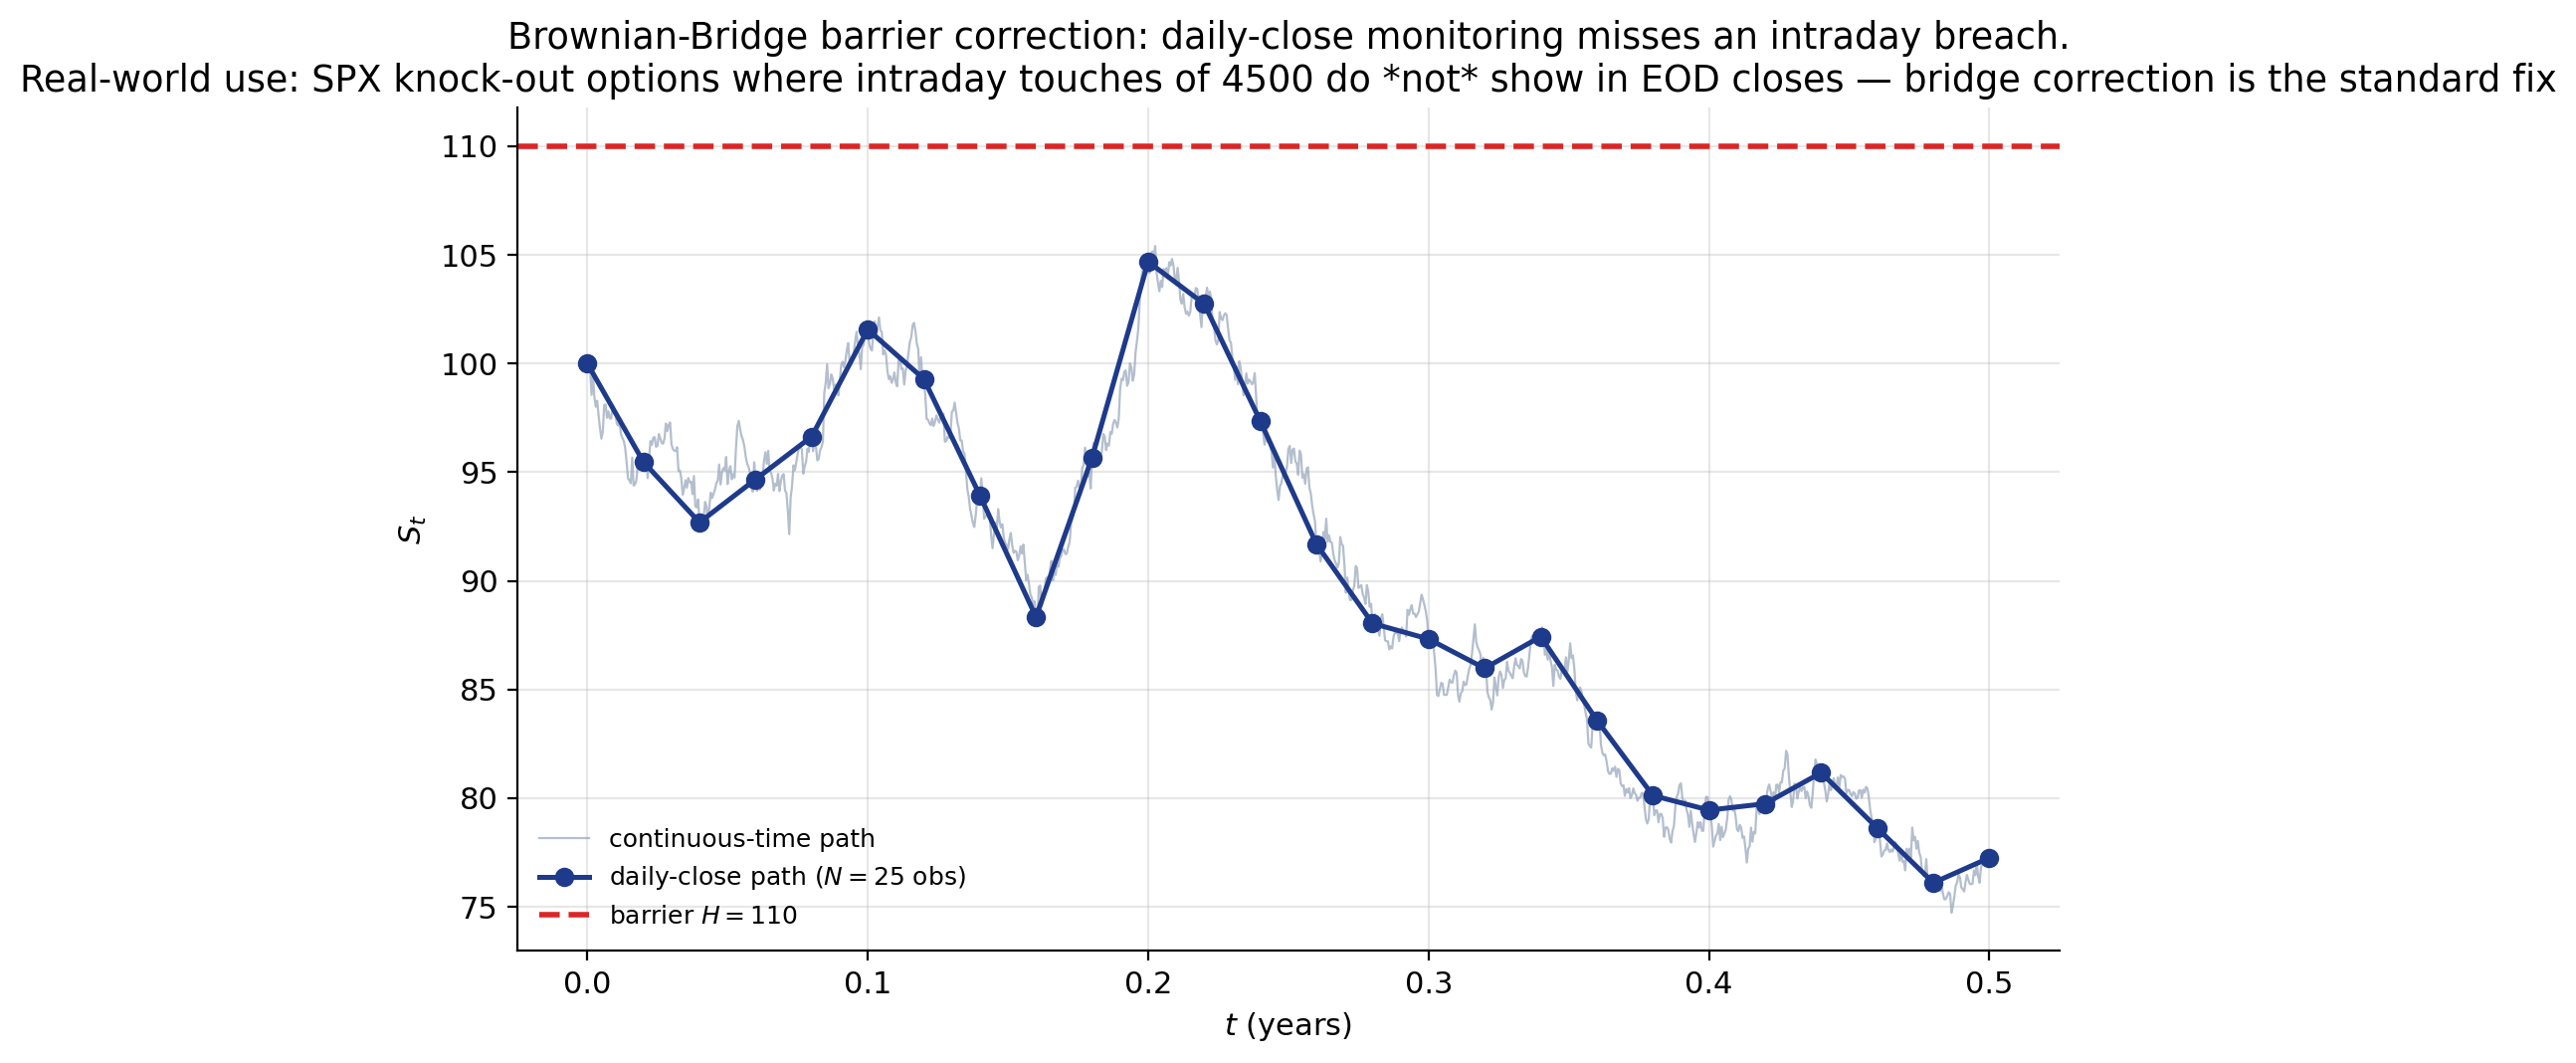
\includegraphics[keepaspectratio]{figures/ch09-bb-barrier.png}}
\caption{Daily-close path (blue dots) that survives a discrete barrier
check vs the underlying continuous path (grey) that did briefly breach.
SPX knock-out options where intraday touches of 4500 do \emph{not} show
in EOD closes are the standard case; the Brownian-Bridge correction is
the production-standard continuity fix}
\end{figure}

\begin{figure}
\centering
\pandocbounded{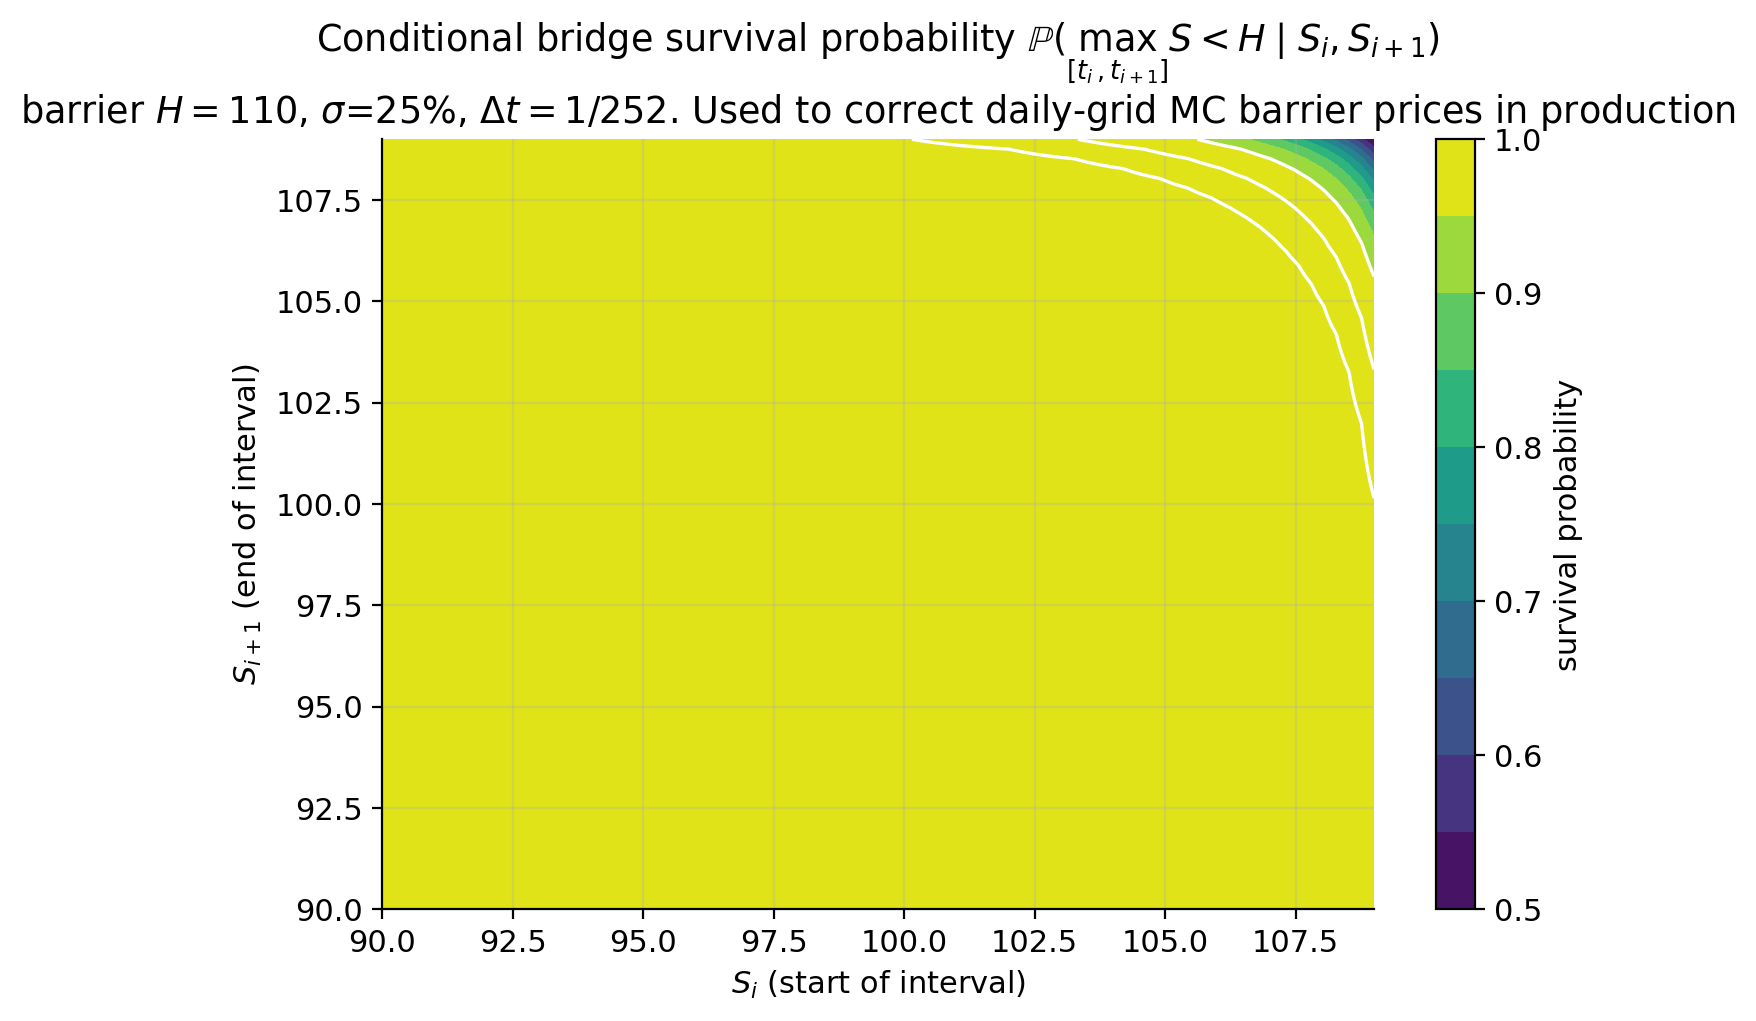
\includegraphics[keepaspectratio]{figures/ch09-bb-survival.png}}
\caption{Conditional bridge survival probability
\(\mathbb{P}(\max_{[t_i, t_{i+1}]} S < H \mid S_i, S_{i+1})\) as a heat
map over the two endpoint values. Survival drops sharply as
\(\max(S_i, S_{i+1}) \to H\) --- the bump that the bridge correction
adds back to the discrete-grid MC estimate}
\end{figure}

Concrete numbers. For the up-and-in call with \(S_0 = 100\),
\(K = 100\), \(U = 110\), \(\sigma = 20\%\), \(r = 5\%\), \(T = 1\) at
\(N = 50\): raw MC gives \(\approx 5.8\); bridge-corrected gives
\(\approx 6.12\), within \(0.5\%\) of the true \(6.15\). The bridge at
\(N=50\) matches brute-force \(N\approx 500\) --- a factor-of-\(10\)
saving.

\subsection{9.7.7 Variance of the barrier
estimator}\label{variance-of-the-barrier-estimator}

The payoff \(X = e^{-rT}(S_T - K)_+\,\mathbf{1}_{\{\max S\ge U\}}\) is
zero on most paths when the barrier is deep OTM, so the estimator is
dominated by a handful of triggering paths. If knock-in probability is
\(p_{\text{knock}}\), the standard error scales as
\(\sqrt{p_{\text{knock}}\,\sigma_X^2/M}\), needing roughly
\(1/p_{\text{knock}}\) more paths than the vanilla case. Rare-event MC
is computationally unforgiving.

Two standard remedies. \emph{Importance sampling} shifts the drift of
the simulation to make knock-in more likely, then reweights by the
Radon--Nikodym derivative (Chapter 5); a well-tuned IS can reduce
variance by factors of \(10\)--\(100\) for deeply out-of-the-barrier
options. \emph{Control variates} using the vanilla European call (whose
expectation is known exactly from (9.14)--(9.15) and whose payoff
correlates strongly with the barrier payoff on paths that do knock in)
provide another order of magnitude of variance reduction for
mildly-barriered options. In production, combining IS with a
vanilla-call control and Brownian-bridge correction can drive barrier-MC
run times from hours to seconds.

\subsection{9.7.8 Other path-dependent
families}\label{other-path-dependent-families}

Having priced barriers, we preview the broader landscape of
path-dependent options that the Monte-Carlo machinery handles cleanly.

\textbf{Asian options.} Payoffs depend on the \emph{average} of the
underlying over a window, such as \((\bar{S}_T - K)_+\) where
\(\bar{S}_T = (1/N)\sum_{n=1}^N S_{t_n}\) (arithmetic average).
Arithmetic Asians have no closed form under GBM because the sum of
log-normals is not itself log-normal; MC is the standard tool. The
corresponding \emph{geometric} average
\(\bar{S}^{\text{geo}}_T = \prod_{n=1}^N S_{t_n}^{1/N}\) \emph{is}
log-normal and admits a closed-form Black--Scholes-style pricer, which
makes it a natural control variate for arithmetic Asian MC --- typical
variance reduction factors of \(50\) to \(500\). Asian options are
popular on commodity markets (oil, gas, metals) because averaging
smooths out daily-price noise and resists single-day manipulation of the
settlement print.

\textbf{Lookback options.} Payoffs depend on the running extremum, such
as \((\max_t S_t - K)_+\) (lookback call on running max) or
\((S_T - \min_t S_t)_+\) (lookback put on running min). Lookbacks are
the most path-sensitive of the classical exotics and carry prices
substantially higher than vanilla equivalents --- they capture the best
achievable entry point, an upper bound on realisable profit. Closed
forms exist under continuous-monitoring GBM (again via the reflection
principle), making lookbacks a useful benchmark for MC implementations.

\textbf{Combinations.} Practitioners layer features routinely --- an
``Asian barrier call'' pays \((\bar{S}_T - K)_+\) but only if the
running max stays below some upper barrier; a ``cliquet with knock-out''
terminates the coupon stream if a down-barrier is hit. These
combinations have no closed form and are handled by MC with custom
payoff functions that walk each path and assemble the appropriate
indicator and averaging structure.

\textbf{Autocallables.} Highly structured products that pay coupons on
observation dates if the underlying is above a specified trigger, and
auto-call (early redemption of principal) once the underlying breaches
an upper barrier. Autocallable pricing involves a mix of
path-dependence, multiple discrete monitoring dates, and
early-termination optionality; MC is the workhorse, typically with
quasi-Monte-Carlo low-discrepancy sequences to reduce variance on the
discrete fixing dates.

All of these families share the same MC machinery: generate paths under
\(\mathbb{Q}\), apply the payoff functional to each path, average with
discount. The engineering art is in (i) reducing variance through
targeted techniques (Asian controls for Asians, bridge corrections for
barriers, importance sampling for rare-event payoffs), (ii) handling the
exact contractual details correctly (continuous vs.~discrete monitoring,
fixed vs.~floating strikes, local vs.~global conditions, business-day
conventions), and (iii) extracting Greeks efficiently from the same
sample.

\begin{center}\rule{0.5\linewidth}{0.5pt}\end{center}

\section{9.8 Variance Reduction: Antithetic and Control
Variates}\label{variance-reduction-antithetic-and-control-variates}

Every production Monte-Carlo pricer uses variance reduction. The
\(M^{-1/2}\) convergence rate is fixed by the central limit theorem, but
the \emph{constant} in front --- the standard deviation
\(\mathrm{sd}(X)\) of the estimator variate --- can be driven down by
orders of magnitude with modest effort. Two techniques are universal:
antithetic variates and control variates. We cover them here as a bridge
to the Heston MC of Chapter 10, where they become essential rather than
merely convenient.

\subsection{9.8.1 Antithetic variates}\label{antithetic-variates}

The antithetic-variates trick exploits the symmetry of the Gaussian
distribution. For each standard-normal draw \(Z^{(m)}\), also use
\(-Z^{(m)}\). The symmetrised payoff is

\[
\widetilde{X}^{(m)} \;=\; \frac{1}{2}\,\bigl[\,X(Z^{(m)}) + X(-Z^{(m)})\,\bigr],
\tag{9.33}
\]

and the antithetic estimator is
\(\widehat{V}_0^{\text{ant}} = (1/M)\sum_m \widetilde{X}^{(m)}\). The
computational cost is \(2M\) payoff evaluations, but the effective
sample size from the variance-reduction standpoint is \emph{not} \(2M\)
--- the two draws \(X(Z)\) and \(X(-Z)\) are \emph{negatively}
correlated, and the variance of the average is

\[
\mathbb{V}[\widetilde{X}^{(m)}] \;=\; \frac{1}{4}\,\bigl[\,\mathbb{V}[X(Z)] + \mathbb{V}[X(-Z)] + 2\,\mathbb{C}[X(Z), X(-Z)]\,\bigr] \;=\; \frac{1}{2}\,\mathbb{V}[X]\,(1 + \rho),
\tag{9.34}
\]

where \(\rho := \operatorname{Corr}(X(Z), X(-Z))\). If \(\rho < 0\), the
variance is strictly less than \(\mathbb{V}[X]/2\), and antithetic
sampling outperforms independent sampling even at equal cost.

When does antithetic sampling work? It works best when the payoff
\(X(Z)\) is \emph{monotone} in \(Z\) --- calls are, puts are (after sign
flip), digitals are, lookbacks almost are. For a monotone increasing
\(X\), \(X(Z)\) and \(X(-Z)\) have correlation close to \(-1\) in the
Gaussian tails, and the variance reduction factor can be substantial.
For a European call at typical ATM parameters, antithetic sampling at
\(M\) pairs typically achieves a variance reduction of about \(2\)
relative to independent sampling at \(M\) pairs (i.e., \(2M\)
independent draws) --- equivalent to halving the standard error for the
same number of payoff evaluations.

\pandocbounded{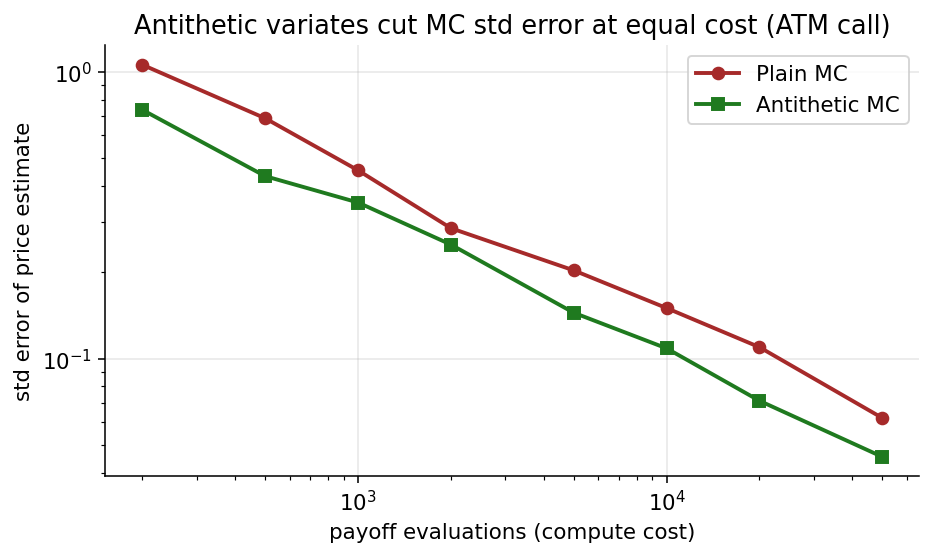
\includegraphics[keepaspectratio]{figures/ch10-antithetic-vs-plain.png}}
\emph{At equal payoff-evaluation cost, antithetic sampling lowers the MC
standard error below plain sampling across every sample size. Both
schemes retain the \(1/\sqrt{M}\) slope --- variance reduction moves the
intercept, not the rate --- and the empirical gap matches the
theoretical factor of \(\sqrt{2}\) for monotone payoffs near ATM.}

Antithetic sampling fails when the payoff is \emph{symmetric in \(Z\)}
--- e.g.~a straddle \(|S_T - K|\) at \(K = S_0 e^{rT}\) gives
\(\rho = +1\) and no reduction. The technique extends naturally to path
simulation by negating the entire Gaussian vector
\((Z_1,\dots,Z_N) \to (-Z_1,\dots,-Z_N)\), and yields similar
factor-of-\(2\)--\(3\) reductions on barriers and Asians.

\begin{figure}
\centering
\pandocbounded{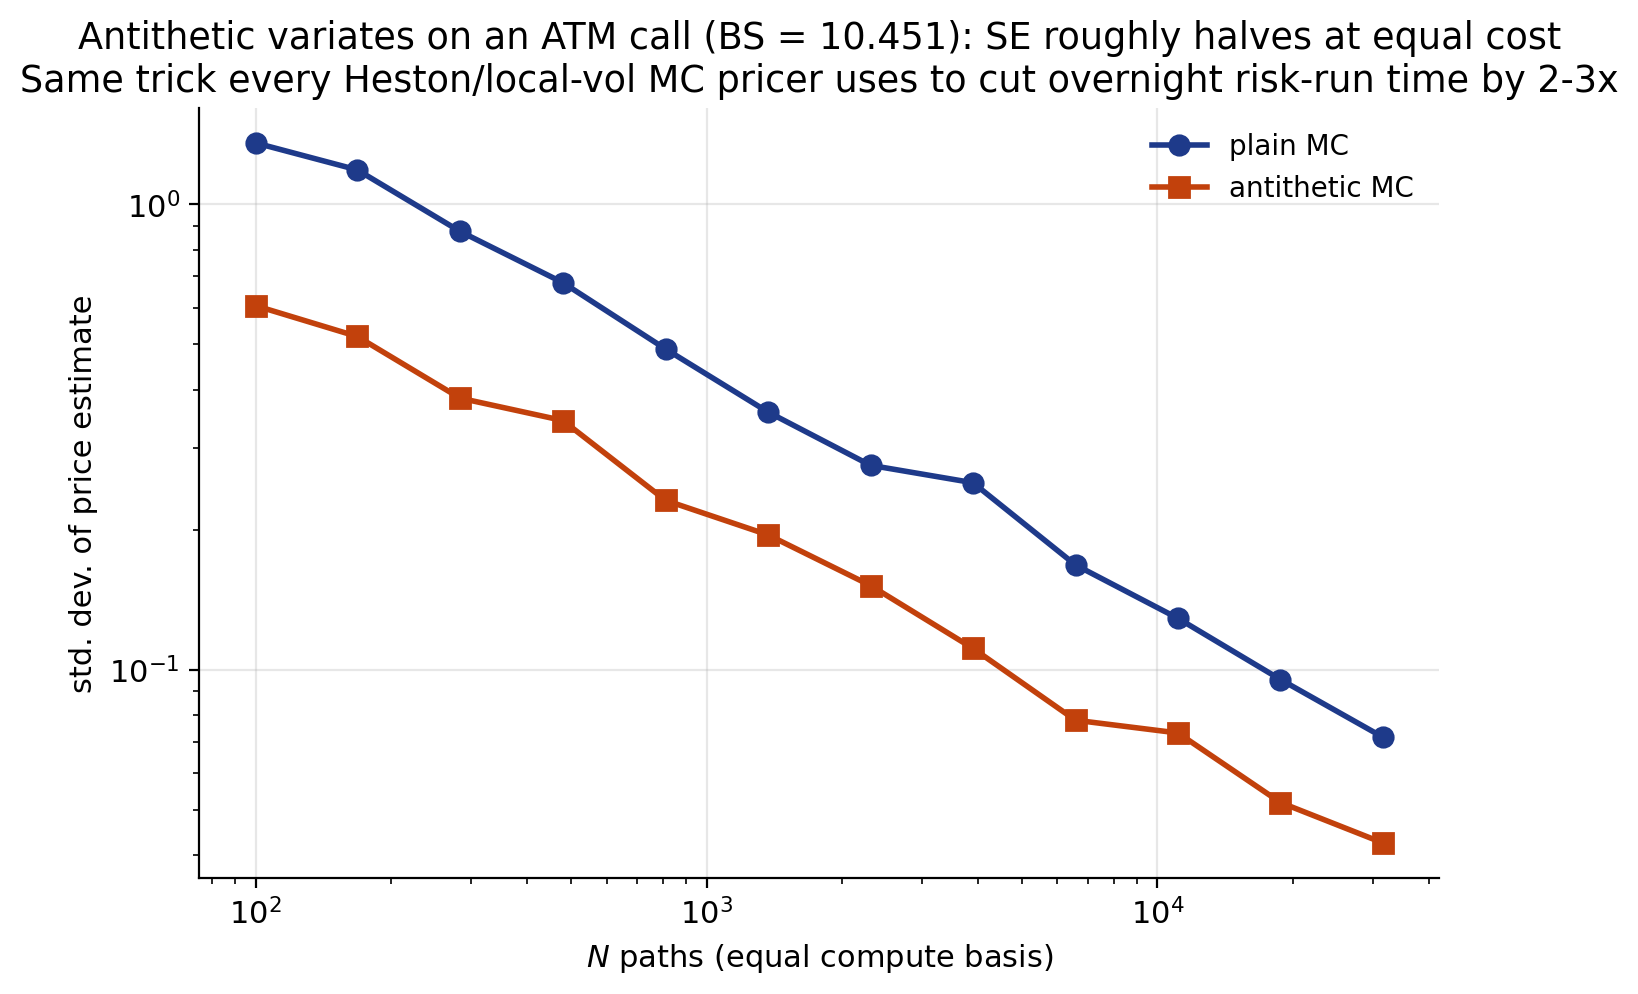
\includegraphics[keepaspectratio]{figures/ch09-antithetic.png}}
\caption{Antithetic versus plain MC on an ATM call across sample sizes:
roughly half the standard error at equal compute. Same trick every
Heston Monte-Carlo overnight risk run uses to keep 99\%-CTE confidence
intervals under desk tolerances}
\end{figure}

\subsection{9.8.2 Control variates}\label{control-variates}

The control-variate trick is more flexible and often more powerful than
antithetic sampling. The idea: find an auxiliary variable \(Y\) that is
strongly correlated with the payoff \(X\) and whose expectation
\(\mathbb{E}[Y]\) is known in closed form. Form the control-variate
estimator

\[
\widehat{V}_0^{\text{cv}} \;=\; \widehat{m}_X \;+\; \beta\,\bigl(\mathbb{E}[Y] - \widehat{m}_Y\bigr),
\tag{9.35}
\]

where \(\widehat{m}_X\) and \(\widehat{m}_Y\) are the sample means of
\(X\) and \(Y\) on the same \(M\) paths, and \(\beta\) is a constant to
be chosen. The estimator is unbiased for any \(\beta\) because
\(\mathbb{E}[\widehat{m}_Y] = \mathbb{E}[Y]\), so the correction term
has mean zero; it has variance

\[
\mathbb{V}[\widehat{V}_0^{\text{cv}}] \;=\; \frac{1}{M}\,\bigl[\,\mathbb{V}[X] \;-\; 2\beta\,\mathbb{C}[X, Y] \;+\; \beta^2\,\mathbb{V}[Y]\,\bigr],
\tag{9.36}
\]

which is minimised at

\[
\beta^{\star} \;=\; \frac{\mathbb{C}[X, Y]}{\mathbb{V}[Y]},
\tag{9.37}
\]

giving the minimum variance

\[
\mathbb{V}[\widehat{V}_0^{\text{cv}}]\bigm|_{\beta = \beta^\star} \;=\; \frac{\mathbb{V}[X]}{M}\,\bigl(1 - \rho_{XY}^2\bigr),
\tag{9.38}
\]

where \(\rho_{XY} = \operatorname{Corr}(X, Y)\). The variance reduction
factor is \(1/(1-\rho_{XY}^2)\): for \(\rho_{XY} = 0.9\) the reduction
is about \(5\times\); for \(0.99\) it is \(50\times\); for \(0.999\) it
is \(500\times\).

Choosing a good control. The essential question is what auxiliary \(Y\)
is known in closed form \emph{and} strongly correlated with the target
payoff. Several standard choices:

\begin{itemize}
\tightlist
\item
  \textbf{The underlying's terminal value \(Y = S_T\)}, with
  \(\mathbb{E}^{\mathbb{Q}}[S_T] = S_0\,e^{rT}\) from the martingale
  property. Works well for European calls and puts, whose payoffs are
  monotone in \(S_T\); typical correlation at ATM parameters is
  \(\rho\approx 0.95\) for calls, giving about a \(10\times\) variance
  reduction.
\item
  \textbf{A vanilla Black--Scholes call on the same underlying}, with
  \(\mathbb{E}[Y]\) given by (9.14)--(9.15). Works extremely well for
  barriers, digitals, and mildly exotic payoffs whose MC error on the
  vanilla portion would otherwise dominate; typical \(\rho\approx 0.99\)
  for up-and-in calls, giving \(50\times\) or more variance reduction.
\item
  \textbf{A geometric-average Asian call} for arithmetic Asian pricing,
  where the geometric version has a closed-form BS-like formula and the
  arithmetic version does not. Typical \(\rho > 0.99\) because the two
  averages are near-identical on almost every path;
  \(100\)--\(500\times\) variance reduction.
\item
  \textbf{The terminal value on a drift-shifted GBM} as a control for
  stochastic-volatility payoffs, linking the Heston case back to the
  Black--Scholes benchmark with matched \(\mathbb{E}[S_T]\) and
  approximate variance.
\end{itemize}

Estimating \(\beta^\star\). The optimal \(\beta^\star\) depends on the
unknown covariance structure. In practice one runs a pilot batch of
\(M_{\text{pilot}} = 1000\) or so paths, estimates
\(\widehat{\beta} = \widehat{\mathbb{C}}[X,Y]/\widehat{\mathbb{V}}[Y]\)
from the pilot, and then runs the full \(M\) batch with that
\(\widehat{\beta}\) plugged into (9.35). The plug-in estimator is no
longer strictly unbiased (because \(\widehat{\beta}\) and
\(\widehat{m}_X\), \(\widehat{m}_Y\) are all correlated through the
data), but the bias is \(O(1/M)\) and negligible relative to the
statistical error. More sophisticated implementations use a two-sample
scheme: estimate \(\widehat{\beta}\) from paths \(1,\dots,M_1\), use
those paths only for the second-stage estimator on paths
\(M_1+1,\dots,M\), and aggregate.

\begin{figure}
\centering
\pandocbounded{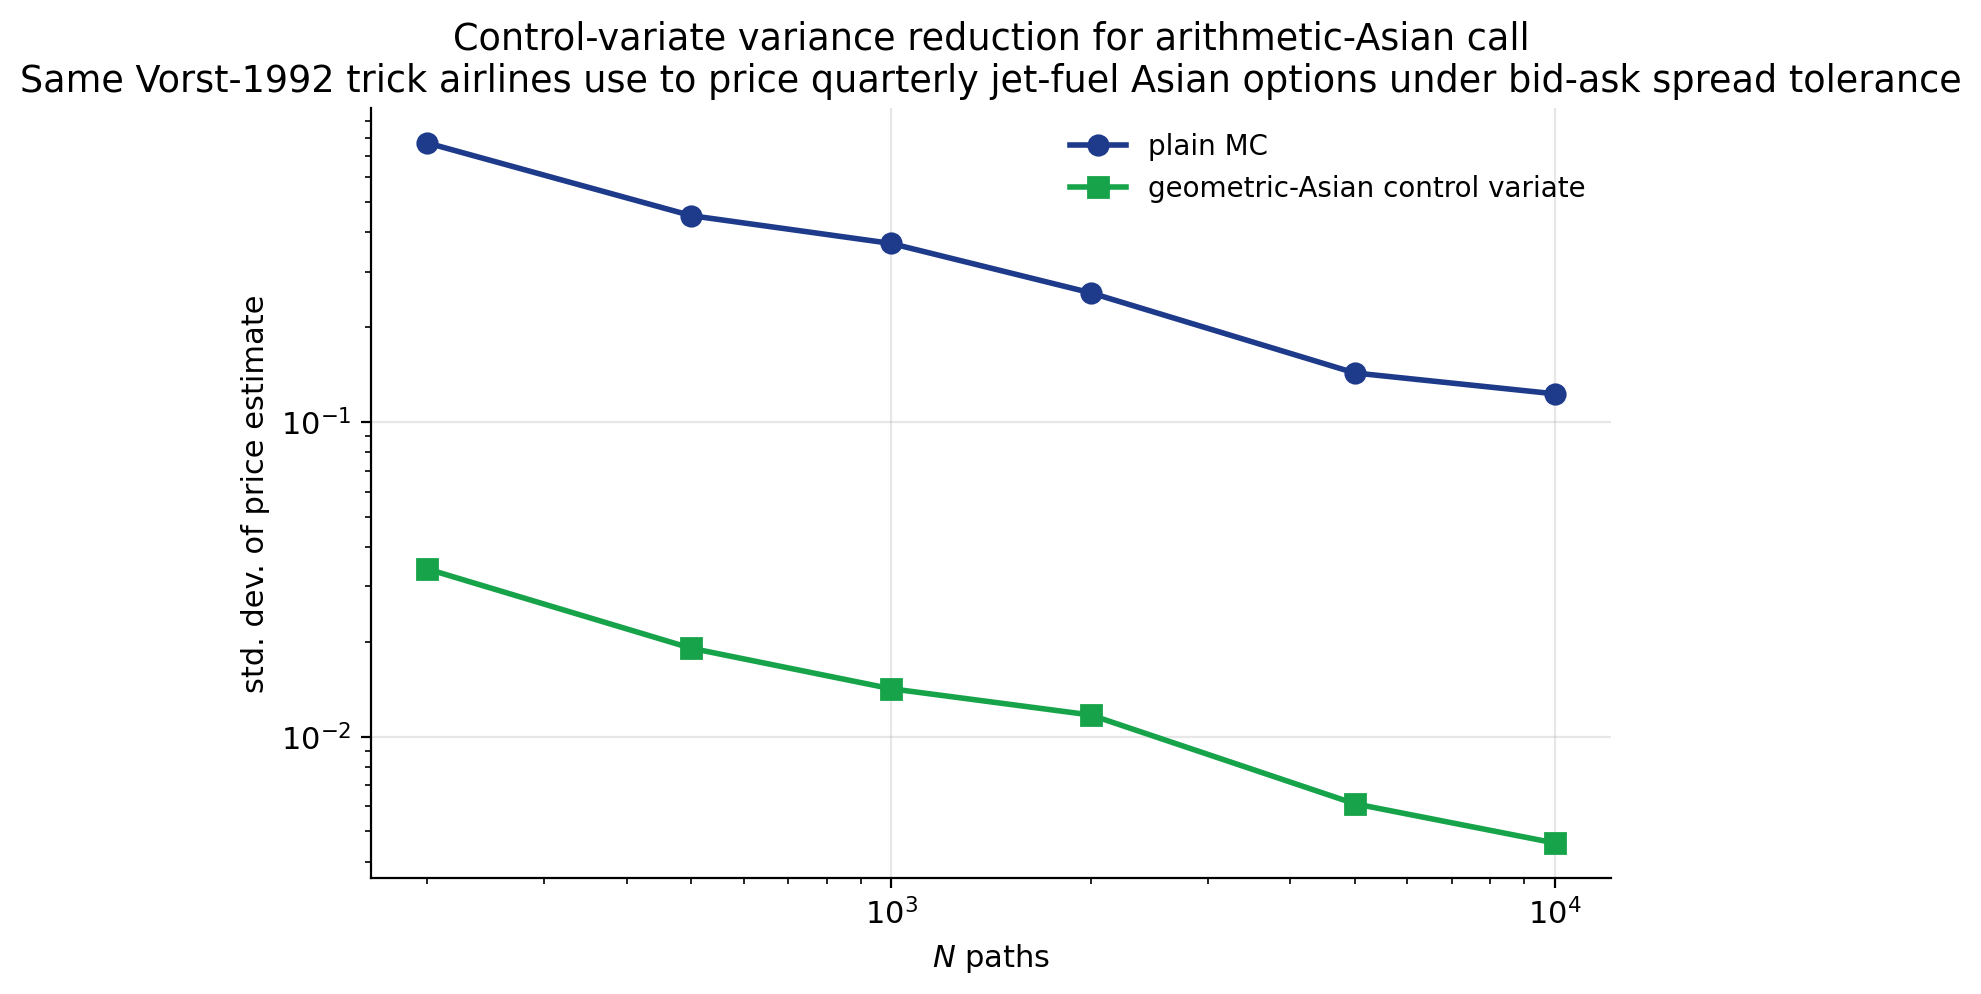
\includegraphics[keepaspectratio]{figures/ch09-control-variate.png}}
\caption{Geometric-Asian control variate cuts the MC standard error for
arithmetic-Asian pricing by an order of magnitude at equal cost. This is
the Vorst (1992) trick that makes jet-fuel quarterly Asian options
tradeable inside airline desk bid-ask spreads}
\end{figure}

\subsection{9.8.3 Combining techniques}\label{combining-techniques}

Antithetic and control variates compose. Apply antithetic sampling to
generate the path pairs, evaluate both the target payoff \(X\) and the
control payoff \(Y\) on each antithetic pair, take the antithetic
average of each, and then apply the control-variate correction (9.35) to
the antithetic averages. The variance reductions multiply roughly (not
exactly, because the correlations interact), and for a European call
with a stock-price control and antithetic draws one routinely achieves
total variance reduction factors of \(30\)--\(50\) at essentially no
added compute cost.

Beyond these two techniques the next layers --- \emph{stratified
sampling} (partitioning the Gaussian space into equal-probability strata
and drawing one sample per stratum), \emph{importance sampling}
(Radon--Nikodym reweighting of the simulation distribution), \emph{Latin
hypercube sampling}, and \emph{quasi-Monte-Carlo with Sobol or Halton
low-discrepancy sequences} --- each provide additional factors of
\(2\)--\(100\) for the right payoff. A production pricer typically
stacks two or three of these techniques; a research-grade pricer may
stack four or five. The trader's mantra: ``MC is universal but wasteful;
always be improving the variance.''

Variance-reduction techniques are indispensable for Heston Monte Carlo
(Chapter 10) where the variance-process simulation itself introduces
additional noise on top of the payoff noise, and where the closed-form
benchmarks from Black--Scholes are no longer available but
\emph{approximate} BS controls based on a matched-moments log-normal
still give large reductions. We return to this theme when we take up
stochastic volatility.

\subsection{9.8.4 Further reading: the wider
toolkit}\label{further-reading-the-wider-toolkit}

Beyond antithetic and control variates, the standard next-layer
techniques are:

\begin{itemize}
\tightlist
\item
  \textbf{Stratified sampling.} Partition the Gaussian space into \(k\)
  equal-probability strata and sample \(M/k\) per stratum. Unbiased,
  never worse than plain MC, but scales poorly with dimension ---
  typically used on the dominant direction only.
\item
  \textbf{Importance sampling.} Reweight by a Radon--Nikodym derivative
  (Chapter 5) to concentrate mass on regions where the payoff is large.
  Variance reductions of \(10\)--\(1000\times\) on rare-event payoffs;
  the technique of choice for deep-OTM options and tail-risk.
\item
  \textbf{Quasi-Monte-Carlo (Sobol, Halton).} Deterministic
  low-discrepancy sequences in place of i.i.d. Gaussians; error scales
  as \(O((\log M)^d/M)\) for smooth integrands. Pairs well with
  scrambling.
\end{itemize}

\pandocbounded{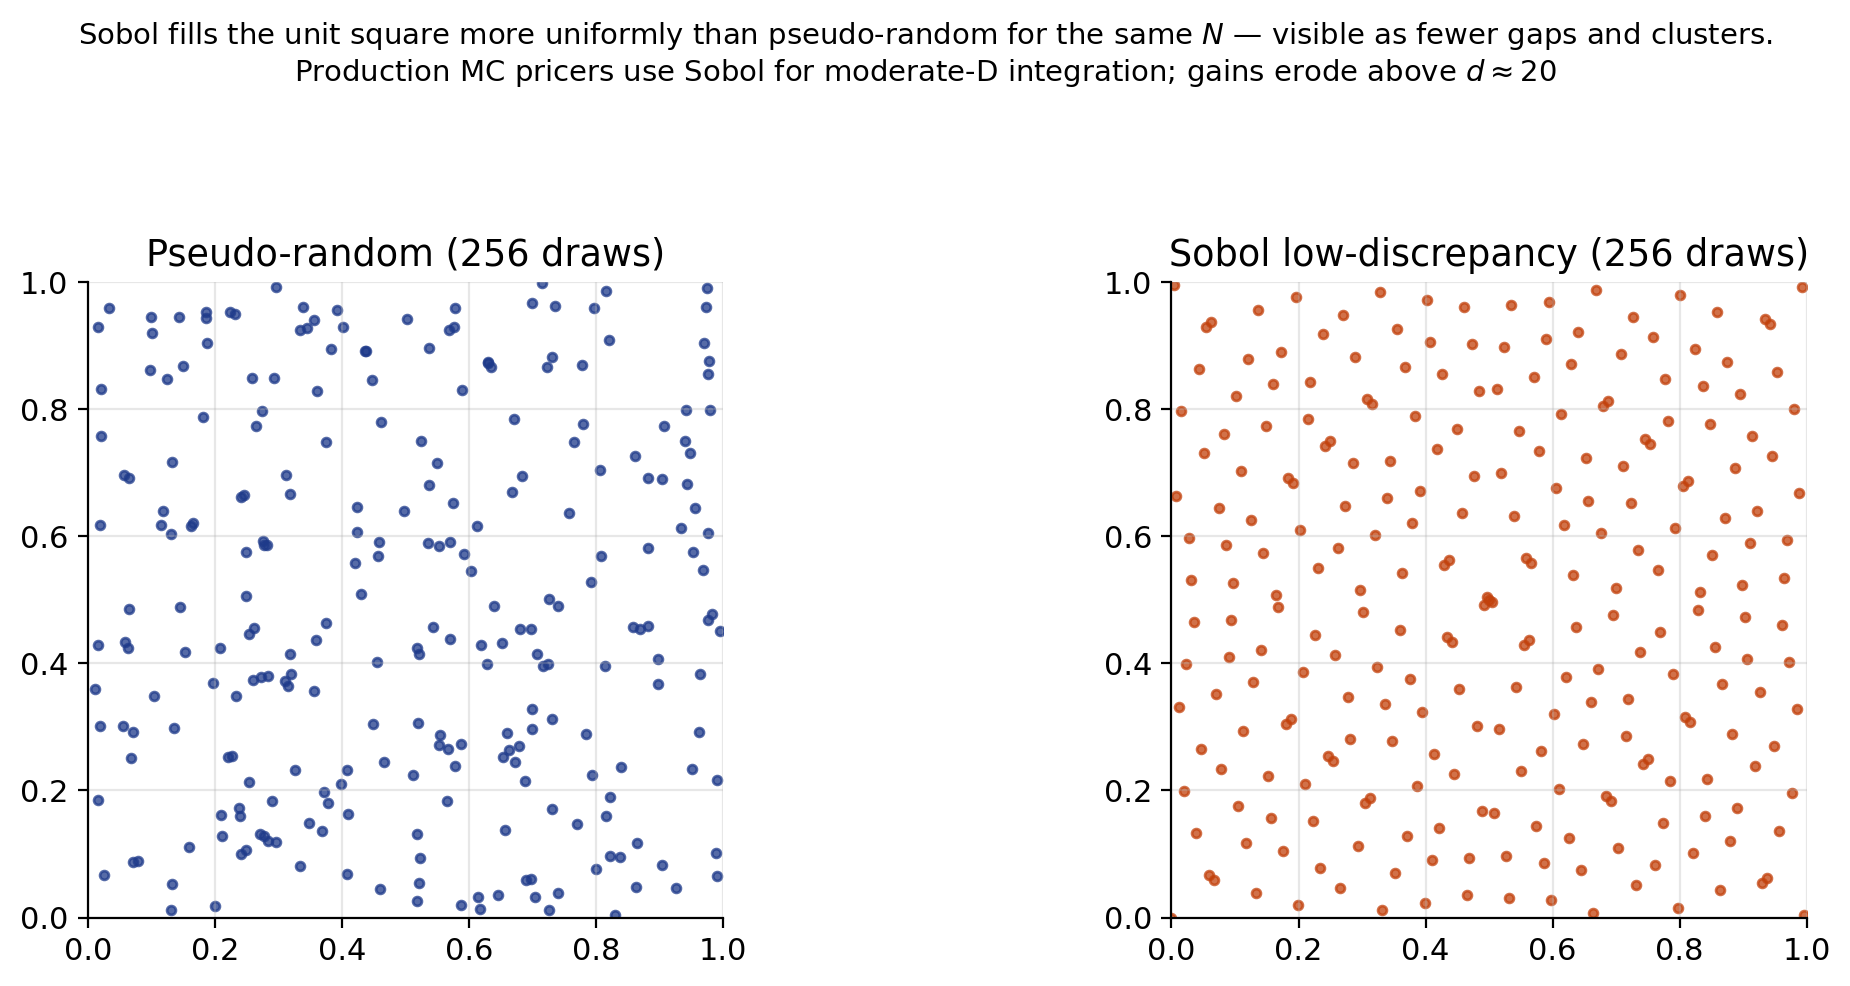
\includegraphics[keepaspectratio]{figures/ch09-sobol-vs-pseudo.png}}
- \textbf{Multilevel Monte Carlo.} Telescoping decomposition across grid
resolutions; reduces total cost for an \(\epsilon\)-accurate estimate
from \(O(\epsilon^{-3})\) to \(\sim O(\epsilon^{-2})\) on
SDE-discretisation-limited problems. - \textbf{Longstaff--Schwartz
regression.} Polynomial regression of continuation values for
American/Bermudan exercise; produces a lower bound on the true price.

Practitioner's rule of thumb: start with antithetic; add a control
variate if a correlated cousin has a closed form; reach for importance
sampling on rare-event payoffs; use Sobol when dimensionality is
moderate and the integrand smooth.

\begin{center}\rule{0.5\linewidth}{0.5pt}\end{center}

\subsection{Case study (a): Asian commodity options on jet
fuel}\label{case-study-a-asian-commodity-options-on-jet-fuel}

\emph{Airlines hedge quarterly fuel cost via average-price calls on jet
kerosene.} \emph{The arithmetic average of correlated lognormals is not
lognormal --- no closed form.} \emph{Production pricer is MC +
geometric-Asian control variate (Vorst 1992).}

\textbf{Context.} Major airlines (Lufthansa, United, Singapore Airlines,
Air France-KLM) hedge between 30--60\% of their forward fuel consumption
at any point through a mix of OTC and listed instruments on jet kerosene
(Platts CIF NWE, Singapore MOPS, US Gulf 54-grade) and proxy hedges in
heating oil and Brent. The standard product is an Asian (average-price)
call: payoff at \(T_2\) equals
\(\max\bigl(\bar S_{[T_1,T_2]} - K, 0\bigr)\) where the average
\(\bar S\) is taken over \(N\) daily Platts fixings between an
observation start \(T_1\) and end \(T_2\) (commonly the calendar
quarter). Averaging is contractually preferred to a single-fix European
because (i) airlines consume fuel daily, so an average payoff matches
the actual hedged exposure, and (ii) a single-day European is exposed to
manipulation of the daily marker assessment. Notional is large: the IATA
jet-fuel hedge volume across the top-20 carriers ran roughly \$50--80B
notional through 2018--19.

The product priced by an airline desk on a typical day will have \(T_2
- T_1 \approx 60\) business days (one quarter), \(N \approx 60\) daily
fixings, \(K\) a few percent in or out of the money relative to the
forward curve, and a \(\sigma\) implied vol on jet fuel in the 20--35\%
range. There is no closed-form European-style pricing formula because
the arithmetic average \(\bar S = \tfrac{1}{N}\sum_n S_{t_n}\) of
correlated lognormals is not itself lognormal: the sum-of-lognormals
distribution has no analytic CDF and, while its first two moments are
available in closed form (Turnbull-Wakeman, Levy moment-matching), the
implied call is only as good as the tail approximation.

\textbf{Reading it through the chapter's math.} Direct application of
the MC estimator (9.10) extended to the path-dependent payoff: generate
\(M\) paths under \(\mathbb{Q}\) with the GBM step (9.9) on a daily grid
covering \([0, T_2]\), evaluate
\(\bar S^{(m)} = \tfrac{1}{N}\sum_{n} S_{t_n}^{(m)}\) on each path, take
\(\hat V_0 = e^{-rT_2}\,\tfrac{1}{M}\sum_m (\bar S^{(m)} - K)_+\). A
naive run with \(M = 10\,000\) paths and \(N = 60\) daily fixings on a
30\%-vol underlying gives a standard error of about 2\% of premium ---
too coarse for a desk that quotes to a half-cent bid-ask. The decisive
trick (§9.8.2) is the Vorst (1992) geometric-Asian control: the
\emph{geometric} average
\(\bar S^{\text{geo}} = \bigl(\prod_n S_{t_n}\bigr)^{1/N}\) \emph{is}
lognormal under GBM (the log of a sum of jointly-normal log-prices is
itself normal), so the geometric-Asian call has a closed-form BS-style
price. Empirically the arithmetic and geometric averages on commodity-
vol paths correlate at \(\rho > 0.998\), giving variance reduction
\(1/(1 - \rho^2) > 250\times\) via (9.35). The same \(M = 10\,000\)
paths with the geometric control cuts the standard error to roughly
0.1\% of premium --- under bid-ask, in production-acceptable wallclock
time (seconds on a single core).

\textbf{Lesson.} Asian options are a clean illustration of the rule that
MC is universal but wasteful, and that a control variate is what makes a
production pricer. The geometric-Asian closed form is not used to price
the contract --- it is used as a noise-reduction device against the
arithmetic-Asian MC estimator. Two operational consequences follow.
First, \emph{always look for a closed-form cousin} of any MC payoff: a
European call on the terminal \(S_{T_2}\) alone (correlation
\(\sim 0.7\)) is a workable backup control when geometric closed forms
are not handy (e.g., basket of correlated commodities). Second, the
variance reduction depends on \(\rho^2\) --- when the control correlates
poorly, adding a second control via multivariate regression (control
matrix) recovers the reduction. The arithmetic-vs-geometric Asian is the
canonical case where a chapter-9 trick converts a two-hour MC run into a
two-second one without changing the underlying physics.

\begin{center}\rule{0.5\linewidth}{0.5pt}\end{center}

\subsection{Case study (b): Autocallable equity
notes}\label{case-study-b-autocallable-equity-notes}

\emph{Path-dependent across multiple observation dates --- closed form
is hopeless.} \emph{Korea, EU, Japan together issue
\textasciitilde\$50B/year of these structured notes.} \emph{Vega term
structure dominates the hedge --- spot delta is the easy part.}

\textbf{Context.} Autocallable notes (also called ``kick-out'' notes,
Phoenix notes, or ``worst-of'' autocallables when written on a basket)
are the single largest category of structured equity products by
issuance volume. A typical retail autocallable on EuroStoxx 50 might pay
an 8\% annualised coupon as long as the index stays above 100\% of
initial on quarterly observation dates; the note auto-calls (returns
principal plus the prevailing coupon) on the first observation where the
index closes above an autocall barrier (often 100\% of initial); and at
the final maturity (commonly 4 to 6 years), if no autocall has occurred
and the index is below a downside knock-in barrier (commonly 60\% of
initial), the investor receives shares at the lower price (or the cash
equivalent). Korean retail issuance alone runs \$20--35B notional/year
through KOSPI 200 and HSCEI-linked ELS (Equity-Linked Securities); EU
private-bank issuance through SG, BNP, Marex, JPM adds another \$20B;
Japanese Uridashi notes add \textasciitilde\$10B. Total street notional
outstanding is in the hundreds of billions and the secondary-market
mark-to-market is a daily MC job for every issuing dealer.

\textbf{Reading it through the chapter's math.} No closed form: the
autocall event depends on the spot trajectory through the discrete
observation dates, the knock-in event depends on the path-minimum
(continuous monitoring on most contracts), and the coupon stream is a
digital-with- recall structure. MC is the only path. Generate \(M\)
paths under \(\mathbb{Q}\) on a daily grid covering the full
\([0, T_{\max}]\) horizon (typically 4--6 years × 252 business days =
1000--1500 steps). On each path, walk through the observation dates in
order: at each date, check the autocall condition; if triggered, accrue
\(e^{-r t_{\text{call}}}\) times the redemption amount, discard the rest
of the path. If never triggered, evaluate the maturity payoff (which
depends on the path minimum vs the knock-in barrier and the terminal
level vs the put strike). Average. Computational cost on a daily grid
for a 5-year autocallable: roughly \(10^5\) paths × \(1.3 \times 10^3\)
steps × four underlyings (a typical worst-of basket) = \(5 \times 10^8\)
Gaussian draws per pricing --- the variance-reduction toolkit
(antithetic + Sobol on observation-date Gaussians, control variates
against the European-equivalent benchmark) is what makes daily MTM
tractable.

\textbf{Lesson.} The pricing is the easy part --- the hard part is the
\emph{hedging}. An autocallable has a non-trivial vega \emph{term
structure}: at inception the issuer is short vega in the early
observation dates (an autocall extinguishes the coupon stream, hurting
the issuer when realised vol is low and the index drifts above the
autocall barrier) and long vega at the terminal maturity (the embedded
down-and-in put benefits the issuer when realised vol is high). The
aggregate Greeks \(\partial V/\partial \sigma_{T_i}\) across observation
dates can flip sign as the spot drifts: a typical Korean ELS book holds
\textasciitilde\$1B of vega notional with sign flips at every
observation date, and a \(1\)-vol-point move in a single tenor on the
vol surface can move book P\&L by tens of millions. Spot delta, by
contrast, is the smoothest Greek in the book (the autocall has bounded
payoff, so \(\Delta\) is bounded by 1 in magnitude). The lesson for the
Chapter-9 reader: when you build a production MC pricer for an
autocallable, the priority is computing the \emph{vega bucket}
sensitivities --- finite-difference \(\partial V/\partial \sigma_{T_i}\)
for each observation tenor --- using common random numbers (CRN) so the
vega-bucket noise is dominated by signal not by MC noise. A book that
hedges the wrong vega tenor is short the right Greek for the wrong
reason and will bleed slowly until the autocall window arrives.

\begin{center}\rule{0.5\linewidth}{0.5pt}\end{center}

\section{9.9 Key Takeaways}\label{key-takeaways-8}

\begin{enumerate}
\def\labelenumi{\arabic{enumi}.}
\item
  \textbf{Why MC.} Monte-Carlo integration escapes the curse of
  dimensionality by achieving \(O(M^{-1/2})\) error \emph{independent of
  dimension}; its cost is \(O(Md)\) compared to \(O(N^d)\) for
  deterministic quadrature. Break-even dimension is around
  \(d\approx 5\), and every realistic path-dependent pricing problem
  lives well above it.
\item
  \textbf{Strong Law of Large Numbers.} For i.i.d. draws of a random
  variable \(X\) with \(\mathbb{E}[|X|]<\infty\), the sample mean
  converges almost surely to \(\mathbb{E}[X]\). For finite-variance
  \(X\), the Central Limit Theorem gives the \(M^{-1/2}\) error rate and
  the basis for confidence intervals.
\item
  \textbf{Standard error.} The MC estimator's standard error is
  \(\widehat{\sigma}_{m_1} = \widehat{s}/\sqrt{M}\), where
  \(\widehat{s}^2 = (1/(M-1))\sum(X^{(m)} - \widehat{m}_1)^2\) is the
  unbiased sample variance. Halving the error bar costs \(4\times\) more
  paths.
\item
  \textbf{Exact GBM generator.} Under \(\mathbb{Q}\), the lognormal
  increment
  \(S_{t_n} = S_{t_{n-1}}\,\exp\{(r-\tfrac{1}{2}\sigma^2)\Delta t_n + \sigma\sqrt{\Delta t_n}\,Z_n\}\)
  with \(Z_n \sim \mathcal{N}(0,1)\) i.i.d. is \emph{exact at the grid
  points} --- no discretisation bias. The
  missing-\(\tfrac{1}{2}\sigma^2\) drift correction is the most common
  bug in home-grown MC pricers.
\item
  \textbf{European MC.} The MC estimator
  \(\widehat{V}_0 = e^{-rT}\cdot (1/M)\sum_m \varphi(S_T^{(m)})\) should
  cross-check against Black--Scholes as a correctness test. At
  \(M = 10{,}000\) and typical ATM parameters, the standard error is
  about \(0.14\) on a call worth about \(10.45\).
\item
  \textbf{Forward-starting (cliquet) atom.} The payoff
  \((S_{T_2} - \alpha S_{T_1})_+\) admits a closed form via iterated
  conditional expectation:
  \(V_0 = S_0\,[\Phi(d_+) - \alpha\,e^{-r(T_2-T_1)}\,\Phi(d_-)]\) with
  \(d_\pm = [\ln(1/\alpha) + (r\pm\tfrac{1}{2}\sigma^2)(T_2-T_1)]/(\sigma\sqrt{T_2-T_1})\).
  The \(S_{T_1}\) factor cancels in the moneyness ratio, making
  \(d_\pm\) deterministic and the price linear in \(S_0\).
\item
  \textbf{Barrier MC.} The up-and-in call payoff
  \((S_T - K)_+\,\mathbf{1}_{\{\max_t S_t \ge U\}}\) is priced by
  simulation on a time grid with \(\max_n S_{t_n}\) substituted for
  \(\max_t S_t\). The substitution introduces a \emph{downward}
  discretisation bias on the order of \(\sqrt{\Delta t}\).
\item
  \textbf{Brownian-bridge correction.} Between two grid points with
  known endpoints, the conditional barrier-crossing probability has a
  closed form
  \(\exp(-2\,\ln(U/S_{t_{n-1}})\,\ln(U/S_{t_n})/(\sigma^2\Delta t_n))\).
  Applying the correction reduces barrier MC bias from
  \(O(\sqrt{\Delta t})\) to \(O(\Delta t^{3/2})\) --- equivalent to a
  factor-of-\(10\) grid refinement.
\item
  \textbf{Rare-event variance.} Barrier payoffs that knock in with small
  probability give MC estimators with large relative variance. The path
  count scales inversely with the knock-in probability, making
  brute-force MC impractical for deeply-barriered structures; importance
  sampling and control variates are essential.
\item
  \textbf{Antithetic variates.} For each \(Z\) draw, also use \(-Z\).
  For monotone payoffs the antithetic pair has strongly negative
  correlation, and the variance of the average is less than half the
  variance of a single draw. Typical variance reduction factor
  \(\approx 2\) on ATM European calls.
\item
  \textbf{Control variates.} Given an auxiliary \(Y\) with known
  \(\mathbb{E}[Y]\), form
  \(\widehat{V}_0^{\text{cv}} = \widehat{m}_X + \beta(\mathbb{E}[Y] - \widehat{m}_Y)\)
  with \(\beta^\star = \mathbb{C}[X,Y]/\mathbb{V}[Y]\). Variance
  reduction factor \(1/(1 - \rho_{XY}^2)\). For \(\rho = 0.99\),
  \(50\times\); for \(\rho = 0.999\), \(500\times\).
\item
  \textbf{Combining techniques.} Antithetic and control variates
  compose; production pricers routinely stack two or three techniques
  for combined variance-reduction factors of \(50\)--\(500\).
\item
  \textbf{Path-dependent families.} Asians, lookbacks, barriers,
  cliquets, autocallables --- all handled by the same MC machinery:
  generate paths under \(\mathbb{Q}\), apply the payoff functional
  path-by-path, discount and average. The engineering difficulty lies in
  variance reduction and in handling the exact contractual conventions
  (continuous vs discrete monitoring, fixed vs floating strikes,
  business-day conventions).
\item
  \textbf{Bridge to Chapter 10.} Heston Monte Carlo introduces a second
  simulation dimension (the variance process) and its own set of
  discretisation biases (the square-root process near zero requires
  careful handling via the full-truncation Euler or the exact QE scheme
  of Andersen). The variance-reduction toolkit developed here transfers
  directly, with BS-based controls replaced by matched-moments lognormal
  controls.
\end{enumerate}

\begin{center}\rule{0.5\linewidth}{0.5pt}\end{center}

\section{9.10 Reference Formulas}\label{reference-formulas-5}

Strong law of large numbers.
\[\lim_{M\to+\infty}\,\frac{1}{M}\sum_{m=1}^{M} X^{(m)} \;=\; \mathbb{E}[X] \quad\text{a.s., provided }\mathbb{E}[|X|]<\infty.\]

Central limit theorem (Monte-Carlo confidence interval).
\[\sqrt{M}\,(\widehat{m}_M - \mathbb{E}[X]) \xrightarrow{d} \mathcal{N}(0,\mathbb{V}[X]), \qquad \widehat{m}_M \pm 1.96\,\widehat{\sigma}_{m_1}\ \text{is a 95\% CI}.\]

Sample mean and Monte-Carlo standard error.
\[\widehat{m}_1 = \frac{1}{M}\sum_{m=1}^M X^{(m)}, \qquad \widehat{\sigma}_{m_1} = \frac{1}{\sqrt{M}}\left(\frac{1}{M-1}\sum_{m=1}^M (X^{(m)} - \widehat{m}_1)^2\right)^{\!1/2}.\]

Exact lognormal GBM path simulation.
\[S_{t_n} = S_{t_{n-1}}\,\exp\!\bigl\{(r - \tfrac{1}{2}\sigma^2)\Delta t_n + \sigma\sqrt{\Delta t_n}\,Z_n\bigr\}, \quad Z_n \stackrel{\text{iid}}{\sim}_{\mathbb{Q}}\mathcal{N}(0,1).\]

European MC estimator.
\[\widehat{V}_0 = e^{-rT}\cdot\frac{1}{M}\sum_{m=1}^M \varphi\!\left(S_0\,e^{(r-\tfrac{1}{2}\sigma^2)T + \sigma\sqrt{T}\,Z^{(m)}}\right).\]

Forward-starting (cliquet) call price.
\[V_0 = S_0\,\bigl[\Phi(d_+) - \alpha\,e^{-r(T_2-T_1)}\,\Phi(d_-)\bigr], \qquad d_\pm = \frac{\ln(1/\alpha) + (r\pm\tfrac{1}{2}\sigma^2)(T_2-T_1)}{\sigma\sqrt{T_2-T_1}}.\]

Up-and-in call payoff and MC estimator.
\[\varphi = (S_T - K)_+\,\mathbf{1}_{\{\max_{0\le t\le T} S_t \ge U\}}, \qquad \widehat{V}_0 = e^{-rT}\cdot\frac{1}{M}\sum_{m=1}^M (S_T^{(m)} - K)_+\,\mathbf{1}_{\{\max_n S_{t_n}^{(m)}\ge U\}}.\]

Brownian-bridge crossing probability (continuous barrier correction).
\[\mathbb{P}\!\left(\max_{t\in[t_{n-1},t_n]} S_t \ge U \,\Big|\, S_{t_{n-1}}, S_{t_n}\right) = \exp\!\left(-\,\frac{2\,\ln(U/S_{t_{n-1}})\,\ln(U/S_{t_n})}{\sigma^2\,\Delta t_n}\right)\quad \text{for } U>\max(S_{t_{n-1}}, S_{t_n}).\]

In-out parity.
\[V^{\text{up-and-in call}} + V^{\text{up-and-out call}} = V^{\text{vanilla call}}.\]

Antithetic variate estimator (single draw).
\[\widetilde{X}^{(m)} = \tfrac{1}{2}\bigl[X(Z^{(m)}) + X(-Z^{(m)})\bigr], \qquad \mathbb{V}[\widetilde{X}^{(m)}] = \tfrac{1}{2}\mathbb{V}[X]\,(1+\rho),\ \rho=\mathrm{Corr}(X(Z), X(-Z)).\]

Control variate estimator and optimal coefficient.
\[\widehat{V}_0^{\text{cv}} = \widehat{m}_X + \beta\bigl(\mathbb{E}[Y] - \widehat{m}_Y\bigr), \qquad \beta^\star = \frac{\mathbb{C}[X,Y]}{\mathbb{V}[Y]}, \qquad \mathbb{V}[\widehat{V}_0^{\text{cv}}]\bigm|_{\beta^\star} = \frac{\mathbb{V}[X]}{M}(1-\rho_{XY}^2).\]

\newpage

\chapter{Chapter 10 --- Heston Stochastic
Volatility}\label{chapter-10-heston-stochastic-volatility}

\emph{Part V opens with the equity-side capstone. Chapter 6 handed us
the Black--Scholes PDE under the assumption that instantaneous variance
\(\sigma^{2}\) is a known constant; every chapter since has carried that
assumption along. The market, of course, does not. Implied-volatility
surfaces slope, twist, and deform in ways that a constant-variance GBM
cannot reproduce. Heston's 1993 model is the cleanest fix: promote the
variance to its own mean-reverting stochastic process, keep tractability
by choosing a square-root (CIR) dynamics for the variance, and pay for
the extra degree of freedom with a second Brownian motion that is
correlated with the underlying. The reward is a semi-closed pricing
formula via Fourier inversion, a genuine stochastic smile, and a hedging
framework that admits volatility as a traded risk factor.}

\emph{This chapter leans on the full Part II toolkit. Two-dimensional
Itô's lemma (Chapter 3) is used in every derivation; multi-dimensional
Girsanov (Chapter 5) is how we move from the physical bivariate SDE to
the risk-neutral dynamics; Feynman--Kac (Chapter 4) underlies the
Riccati ODE system for the characteristic function; and the GBM /
Black--Scholes machinery of Chapter 6 is the benchmark we compare
against. Monte Carlo variance-reduction techniques introduced in Chapter
9 resurface when we discuss simulation-based Heston pricing. The chapter
is almost entirely self-contained analytically, but pedagogically it is
the payoff for Parts II and III.}

\begin{center}\rule{0.5\linewidth}{0.5pt}\end{center}

\section{Chapter map}\label{chapter-map}

\begin{enumerate}
\def\labelenumi{\arabic{enumi}.}
\tightlist
\item
  \textbf{§10.1 Bivariate SDE} --- motivation, specification, and what
  each parameter controls.
\item
  \textbf{§10.2 Feller condition} --- when variance stays strictly
  positive.
\item
  \textbf{§10.3 Change of measure} --- market price of variance risk,
  risk-neutral drift adjustments, uniqueness failure and calibration
  implications.
\item
  \textbf{§10.4 Implied volatility} --- why constant-\(\sigma\) GBM is
  inadequate and what shapes a stochastic-vol model must generate.
\item
  \textbf{§10.5 Characteristic function} --- Riccati ODE derivation for
  the log-price characteristic function.
\item
  \textbf{§10.6 Fourier-inversion pricing} --- recovering \(P_{1}\) and
  \(P_{2}\) and assembling the call price.
\item
  \textbf{§10.7 Greeks and calibration} --- delta, vega, the two extra
  vol-of-vol and correlation sensitivities, calibration workflow.
\item
  \textbf{§10.8 Variance swaps} --- a pure-variance product that prices
  by expectation under \(\mathbb{Q}\).
\item
  \textbf{§10.9 Worked example} --- a numerical Heston
  vs.~Black--Scholes comparison.
\item
  \textbf{§10.10--§10.10B Limitations, comparisons, and extensions.}
\item
  \textbf{§10.11 Key takeaways}, \textbf{Appendix A} (reference
  formulas), and \textbf{Appendix B} (VIX vs SPX historical correlation
  study).
\end{enumerate}

\begin{center}\rule{0.5\linewidth}{0.5pt}\end{center}

\section{10.1 Bivariate SDE ---
motivation}\label{bivariate-sde-motivation}

The Black--Scholes world is complete: a constant volatility \(\sigma\)
plus the bank account span every contingent claim. Empirically, option
markets violate this --- implied vol exhibits a smile / skew across
strike and a term structure across maturity. The Heston (1993) model is
the canonical fix: promote the variance \(v_t\) to its own
mean-reverting square-root SDE, correlate it with the spot, and retain
semi-closed-form pricing via a characteristic function. This chapter
rebuilds the derivation from first principles --- bivariate SDE \(\to\)
Feller condition \(\to\) change of measure with market price of variance
risk \(\to\) characteristic-function ansatz \(\to\) Riccati ODEs \(\to\)
Fourier-inversion pricing (the \(P_1, P_2\) probabilities) --- and
finishes with calibration / Greeks notes and variance swaps.

The post-1987 equity smile is the empirical motivation. Pre-crash
surfaces were reasonably flat; the crash and the rapid revaluation of
tail risk created the persistent left skew that defines equity vol to
this day. Two responses emerged: Dupire's local-vol (exact surface fit
but unrealistic forward smile) and Heston (independent variance SDE with
realistic forward dynamics and a tractable characteristic function via
the affine structure). Heston sits between local-vol and the modern
rough-vol family as the pedagogical and practical baseline.

\subsection{10.1.1 Why stochastic vol produces a
smile}\label{why-stochastic-vol-produces-a-smile}

A Black--Scholes lognormal has a single scale parameter \(\sigma\): the
risk-neutral density of \(\ln X_T\) is a tidy Gaussian with one
variance. Under Heston the conditional density (conditioning on the
whole path of \(v_t\)) is still lognormal --- but the mixture over the
\(v\)-path puts weight on very quiet and very loud regimes, producing
fatter tails than a single lognormal. Fatter tails \(\to\) deep OTM
options are worth more than BS would suggest \(\to\) inverted BS gives
higher implied vols at the wings. The non-zero \(\rho\) then
asymmetrises that mixture: when spot falls, the vol tends to spike (for
\(\rho<0\)), which loads the left tail more than the right. This is the
skew. In short: \(\alpha\) (vol-of-vol) controls the wings (curvature /
smile); \(\rho\) controls the slope (skew); \(\kappa\) controls how
quickly the term-structure of smile flattens; \(\theta\) anchors
long-dated ATM; \(v_0\) anchors short-dated ATM.

\textbf{Mixture intuition.} Heston is Black-Scholes with a stochastic
volatility ``dial'' \(v_t\) --- mean-reverting toward \(\theta\),
perturbed by \(\alpha\sqrt{v}\,\mathrm{d}W^v\), and correlated to spot
with \(\rho\). The terminal distribution of \(\ln F_T\) is a continuous
mixture of lognormals indexed by the path of \(v\); mixing fatness
creates the smile, and the spot-vol correlation tilts it into a skew.

Heston is also the canonical \emph{affine} model: drift and
diffusion-covariance are linear in \((F, v)\), so the characteristic
function solves a finite-dimensional Riccati ODE system regardless of
state-space dimension. The same affine structure underlies CIR
short-rate models, Duffie-Pan-Singleton jump-diffusions, and CIR-style
credit intensities.

\subsection{10.1.2 FTAP recap and
incompleteness}\label{ftap-recap-and-incompleteness}

No arbitrage \(\iff\) there exists a measure
\(\mathbb{Q} \sim \mathbb{P}\) such that all tradeables \(f_t / M_t\)
are \(\mathbb{Q}\)-martingales. This holds always. The measure is unique
only if the market is complete; in incomplete markets (like stochastic
vol) there is no unique \(\mathbb{Q}\).

FTAP I (Chapter 5) gives existence of \(\mathbb{Q}\) iff no arbitrage;
FTAP II gives uniqueness iff the market is complete. Heston has two risk
factors (\(W^F, W^v\)) but only one tradable risk-bearing asset (\(F\));
the rank mismatch makes the market incomplete, and there is a
one-parameter family of risk-neutral measures parameterised by the
market price of variance risk. Calibration ``identifies which
\(\mathbb{Q}\) is currently consistent with observed option prices'';
the gap between \(\mathbb{P}\)-parameters (from returns) and
\(\mathbb{Q}\)-parameters (from options) is the variance risk premium.

To make this concrete, consider what ``hedging'' even means in an
incomplete market. In Black--Scholes, for any contingent claim
\(f(S_T)\), there exists a self-financing strategy
\((\Delta_t, \beta_t)\) in spot and bank that replicates \(f\) exactly
at every time and in every scenario --- zero residual risk. You can
therefore price \(f\) by the no-arbitrage principle: its price must
equal the cost of constructing the replicating portfolio. In Heston, no
such exact replication exists using spot and bank alone. If you run a
delta-hedge based on spot only, you will be exposed to variance
innovations; your hedged portfolio will have residual P\&L proportional
to the vega times the variance shock. The best you can do with spot
alone is minimise some residual-risk metric --- variance-of-P\&L, say
--- but you cannot eliminate it. To eliminate it, you must add another
hedging instrument that is sensitive to variance --- typically another
option --- but then you need that option to be priced, which requires a
model, which requires a \(\mathbb{Q}\), and we are back to the choice
problem.

The resolution in practice is to assume (or impose) a specific choice of
\(\mathbb{Q}\), calibrate it to observed option prices (so that the
market's implied \(\lambda^v\) is respected by construction), and then
perform hedging in a model-consistent way. This is called ``hedging
under the calibrated measure'' and it is what every vol desk does
implicitly. The hedges are not perfect --- they are model hedges --- and
the residual P\&L reflects model risk rather than pure
incompleteness-risk. But the framework at least gives you a coherent way
to think about hedging and risk.

There is a philosophical point here that is easy to miss. In a complete
market, the ``price'' of a contingent claim is unambiguous --- it is the
replication cost. In an incomplete market, ``price'' is an economic
concept, determined by demand and supply, risk preferences, and market
frictions. The model gives you a framework for representing those
ingredients compactly (via the choice of \(\mathbb{Q}\)), but the model
does not determine the price on its own. This is why calibration, rather
than pure derivation, is the central activity of a stochastic vol
practitioner: the prices exist because people trade, and the model is
merely the language in which those prices are expressed.

\subsection{10.1.3 From Black--Scholes drift to the bivariate
SDE}\label{from-blackscholes-drift-to-the-bivariate-sde}

Under \(\mathbb{P}\), a risky asset \(X_t\) that is traded satisfies \[
\mathrm{d}X_t = \mu_t\,\mathrm{d}t + \sigma_t\,\mathrm{d}\tilde{W}_t^{\mathbb{P}},
\qquad \frac{f_t}{M_t} = \mathbb{E}^{\mathbb{Q}}\!\left[\frac{f_T}{M_T}\right],
\tag{10.1}
\] and the \(\mathbb{P}\)-Brownian motion is linked to the
\(\mathbb{Q}\)-Brownian motion by \[
\mathrm{d}\tilde{W}_t = \lambda_t\,\mathrm{d}t + \mathrm{d}W_t^{\mathbb{Q}}.
\tag{10.2}
\] Substituting, \[
\mathrm{d}X_t = (\mu_t - \lambda_t\sigma_t)\,\mathrm{d}t + \sigma_t\,\mathrm{d}W_t^{\mathbb{Q}},
\tag{10.3}
\] where \(\lambda_t\) is the market price of risk. If \(X\) is itself
traded, then under \(\mathbb{Q}\) its drift must be \(r X_t\), pinning
down \(\mu_t - \lambda_t \sigma_t = r X_t\). This is precisely the
Girsanov shift derived in Chapter 5 --- the Radon--Nikodym density
\(Z_t = \exp\!\bigl(-\int_0^t\!\lambda_s\,\mathrm{d}\tilde{W}_s^{\mathbb{P}}
- \tfrac{1}{2}\!\int_0^t\!\lambda_s^{2}\,\mathrm{d}s\bigr)\) is what
converts the \(\mathbb{P}\)-drift into the \(\mathbb{Q}\)-drift, state
by state. The reader who wants the full derivation should consult
Chapter 5 §5; we use the conclusion here.

Read this shift intuitively. Under the physical measure \(\mathbb{P}\),
the asset drifts at its expected return, which includes a risk premium
over the risk-free rate --- that is how risky assets compensate their
holders for bearing risk. The change of measure does not change any
actual path; it rebalances probability weight toward the states that
have been systematically overweighted by risk aversion. Under
\(\mathbb{Q}\), the asset appears to drift at \(r\) because the premium
has been re-absorbed into the measure. The same logic applies --- but
now in two dimensions --- when we introduce stochastic variance.

Here is another way to see it. Imagine running Monte Carlo simulation of
the spot under \(\mathbb{P}\) and under \(\mathbb{Q}\). The individual
paths look similar --- in fact, on any individual path, the realisation
of the Brownian motion is the same (Girsanov tells us that the path
spaces are essentially isomorphic). What differs is the weight that each
path carries in the expectation. Under \(\mathbb{P}\), the ``good''
paths (with high realised returns) have high probability; under
\(\mathbb{Q}\), those good paths are weighted less because risk-averse
investors have bid up their prices (making them seem less attractive
from the valuation standpoint). The effect is that
\(\mathbb{Q}\)-expectations come out lower for linear payoffs on risky
assets than \(\mathbb{P}\)-expectations, which is exactly the
``risk-free rate'' drift you would expect. None of this is about the
trajectory of any particular path; it is all about the measure.

The famous economic interpretation is in terms of pricing kernels or
stochastic discount factors. The Radon--Nikodym derivative
\(\mathrm{d}\mathbb{Q}/\mathrm{d}\mathbb{P}\) is essentially
proportional to a representative investor's marginal utility --- a
number that is high in bad states of the world (when investors value an
extra dollar most) and low in good states. Discounting payoffs by this
kernel and taking a \(\mathbb{P}\)-expectation is equivalent to taking a
\(\mathbb{Q}\)-expectation and discounting by the risk-free rate.
Derivatives pricing in incomplete markets is thus fundamentally linked
to asset-pricing theory: different measures correspond to different
assumptions about the representative investor's risk aversion and
preferences. When you calibrate Heston to market prices, you are
implicitly inferring what marginal utility looks like in the vol
dimension --- at least in the part of the state space where liquid
options exist to probe.

\textbf{Futures.} For a futures price \(F_t\), the Black (1976) argument
(Chapter 8) gives under \(\mathbb{Q}\) \[
\frac{\mathrm{d}F_t}{F_t} = \sigma\,\mathrm{d}W_t^{\mathbb{Q}},
\qquad \text{(Black model for futures prices)}.
\tag{10.4}
\] Under \(\mathbb{P}\), \[
\frac{\mathrm{d}F_t}{F_t} = \mu_t\,\mathrm{d}t + \sigma\,\mathrm{d}W_t^{\mathbb{P}}.
\tag{10.5}
\]

We work in the futures frame partly out of convenience --- futures are
martingales under the risk-neutral measure with no drift to carry around
--- and partly because it highlights the key point that the volatility
structure is what distinguishes Heston from Black, not the drift. The
drift in the risk-neutral world is pinned down by arbitrage; the
interesting degree of freedom is the stochastic behaviour of the
diffusion coefficient.

The practical virtue of the futures-price framework goes beyond
cleanliness. For index and equity markets, listed options actually
expire on forward-contract-settled underliers or near-dated futures; for
FX options, the relevant underlier is a forward rate; for commodity
options, the entire pricing paradigm is built on futures rather than on
any elusive ``spot'' price. So Black (1976) is not a toy simplification
--- it is the framework that actually prices the bulk of liquid options
traded globally. Heston's original 1993 paper followed the Black
tradition (although Heston expressed things in terms of spot with carry;
the two are isomorphic), and the industry has largely standardised on
the futures-frame parameterisation. When a practitioner says
``\(\mathrm{d}F/F = \sqrt{v}\,\mathrm{d}W\),'' they are stating the
Heston--Black benchmark dynamics that underlie essentially every vanilla
calibration you will encounter. Even when the underlying is a spot
rather than a futures, the drift term \(r - q\) (rate minus dividend
yield) can be absorbed into the forward price, and the residual dynamics
look like (10.4) with no drift. In other words: by working in the
futures frame, you focus the analysis exactly on what makes Heston
different from Black--Scholes --- the diffusion \(\sqrt{v_t}\) --- and
defer all drift-related complications to a thin wrapper around the core
SDE.

\subsection{10.1.4 The Heston bivariate
system}\label{the-heston-bivariate-system}

We want to correct for stochastic volatility. Replace the constant
\(\sigma\) by \(\sqrt{v_t}\) and give \(v_t\) its own SDE: \[
\boxed{\;
\frac{\mathrm{d}F_t}{F_t} = \mu_t\,\mathrm{d}t + \sqrt{v_t}\,\mathrm{d}W_t^{\mathbb{P},F}
\;}
\tag{10.6}
\] \[
\boxed{\;
\mathrm{d}v_t = \kappa^{\mathbb{P}}\!\left(\theta^{\mathbb{P}} - v_t\right)\mathrm{d}t + \alpha\sqrt{v_t}\,\mathrm{d}W_t^{\mathbb{P},v}
\;}
\tag{10.7}
\] with \[
\mathrm{d}W_t^{\mathbb{P},F}\cdot \mathrm{d}W_t^{\mathbb{P},v} = \rho\,\mathrm{d}t,
\qquad (W^{\mathbb{P},F}, W^{\mathbb{P},v}) \text{ correlated}.
\tag{10.8}
\]

Look carefully at the choice \(\sqrt{v_t}\) for the diffusion
coefficient. It is not incidental. Modelling in the variance rather than
in the volatility pays two dividends. First, the variance is the natural
additive quantity: variances of independent returns add, volatilities do
not, and any equation that treats variance linearly will be cleaner than
the equivalent vol-level equation. Second, the square-root CIR diffusion
\(\alpha\sqrt{v_t}\,\mathrm{d}W^v\) has the beautiful property that its
diffusion coefficient vanishes as \(v_t \to 0\), which acts as a soft
floor: a variance that wanders toward zero stops diffusing and is pulled
back up by the mean-reversion drift. This is how Heston constructs a
process that stays non-negative under mild parameter conditions, without
resorting to reflecting barriers or hard truncations.

Contrast this with the SABR alternative. SABR models the instantaneous
vol (not variance) with lognormal dynamics:
\(\mathrm{d}\sigma_t = \alpha \sigma_t\,\mathrm{d}W^\sigma\). Lognormal
vol automatically stays positive, which is appealing, but the tradeoff
is that SABR dynamics are not affine, and SABR does not admit a
closed-form characteristic function. Instead, SABR is typically priced
via Hagan's asymptotic expansion --- an approximation that works
brilliantly for short maturities and ATM moneyness but degrades at wings
and long dates. Heston gives up lognormal positivity in exchange for the
affine structure, and the square-root floor on the CIR process is the
mathematical trick that makes this exchange work. Either choice is
defensible; both dominate naive alternatives like an arithmetic Brownian
motion on vol (which can go negative and cannot be rescued by any
floor).

A subtle point about (10.6): the spot is driven by
\(\sqrt{v_t}\,\mathrm{d}W^F\), not by \(\sqrt{v_t}\,\mathrm{d}t\) plus
\(\mathrm{d}W^F\) with some scaling. The diffusion coefficient is a
random function of \(v_t\), which is itself stochastic. This is what
makes the spot a ``stochastic-volatility'' process rather than a
``time-changed'' Brownian motion. Equivalently, you can think of spot's
log-returns as Brownian motion scaled at each instant by \(\sqrt{v_t}\):
when \(v_t\) is high, returns are more volatile; when \(v_t\) is low,
returns are calmer. The picture to keep in mind is a Brownian motion
whose clock speed is itself random, fluctuating between slow and fast
phases. This is not a metaphor --- there is a formal equivalence between
stochastic vol processes and time-changed Brownian motions, where the
time change is the integrated variance. Ocone's representation of
continuous local martingales makes this precise. For our purposes, it
means that many results about Brownian motion carry over to Heston's
log-price after a random time change.

Reading off (10.7):

\begin{itemize}
\tightlist
\item
  \(\kappa^{\mathbb{P}}\) --- mean-reversion rate of variance.
\item
  \(\theta^{\mathbb{P}}\) --- mean-reversion level (long-run variance).
\item
  \(\alpha\) --- vol-of-vol.
\item
  \(\rho\) --- spot/vol correlation (empirically negative for equity
  indices --- the ``leverage effect'').
\item
  The \(\sqrt{v_t}\) diffusion is the CIR / square-root form: such
  processes are called Feller processes.
\end{itemize}

Each of these has an economic interpretation worth lingering over. The
mean-reversion rate \(\kappa\) answers the question, ``if volatility is
currently elevated, how quickly does the market expect it to return to
normal?'' A large \(\kappa\) corresponds to a rubber-band variance that
snaps back quickly --- news-driven spikes fade within days. A small
\(\kappa\) corresponds to a sticky variance that can stay elevated for
quarters or years. The long-run level \(\theta\) is what volatility
reverts to --- the ``cruising altitude'' of the market. For broad equity
indices, \(\theta\) calibrated over long histories tends to land in the
territory of 20\%--25\% annualised vol, which is roughly the long-run
average of realised equity vol.~The vol-of-vol \(\alpha\) governs how
chaotic the variance itself is --- whether the vol process is a gentle
drift or a ragged, spiky trajectory. It is essentially a measure of how
confident the market is in its current vol estimate; higher \(\alpha\)
means the market allows more probability mass on extreme vol regimes.

To calibrate these parameters against historical intuition: typical
calibrated values for a liquid equity index are
\(\kappa \approx 2\text{--}6\) year\(^{-1}\), giving a half-life of vol
shocks of roughly one to four months;
\(\theta \approx 0.04\text{--}0.06\), corresponding to a long-run ATM
vol of 20\%--25\%; \(\alpha \approx 0.4\text{--}1.0\), varying with
market regime; \(\rho \approx -0.6\) to \(-0.8\), stubbornly negative;
and \(v_0\) matching whatever ATM implied vol is currently trading.
These are broad ranges; different asset classes and different volatility
regimes produce quite different calibrated values. Single-stock options
typically show larger \(\alpha\) and \(\theta\) than index options
because single names have more idiosyncratic vol.~Sector ETFs fall in
between. Currency pairs have much smaller \(\alpha\) and less negative
(sometimes near-zero) \(\rho\). Commodities vary wildly by underlier;
storable commodities like gold behave more like FX, while seasonal
commodities like natural gas can exhibit seasonal patterns in \(\theta\)
itself.

The timescale interpretation of \(\kappa\) deserves a second look.
Because \(\kappa\) has units of inverse time, the product
\(\kappa \tau\) is a dimensionless ``time to mean revert.'' When
\(\kappa \tau \ll 1\) (short maturity relative to mean-reversion
timescale), the variance has not had time to converge toward \(\theta\),
and the option's pricing is dominated by the starting variance \(v_0\).
When \(\kappa \tau \gg 1\) (long maturity), the variance has relaxed to
its long-run mean \(\theta\), and the option's pricing is dominated by
\(\theta\) rather than \(v_0\). The crossover between these two regimes
happens around \(\kappa \tau \approx 1\), which for \(\kappa = 2\) is
roughly six months. This is why short-dated and long-dated options carry
quite different parameter-sensitivity fingerprints: short-dated options
are sensitive to \(v_0\) and \(\alpha\); long-dated options are
sensitive to \(\theta\) and \(\kappa\). A good calibration uses this
structural difference to separate the parameters cleanly.

The correlation \(\rho\) is perhaps the most interesting parameter. For
equity indices it is strongly negative --- typically in the range
\(-0.6\) to \(-0.8\) after calibration --- because of what practitioners
call the leverage effect: as the stock price falls, the debt-to-equity
ratio of the underlying firm rises mechanically, making the equity more
levered and therefore more volatile. There is also a behavioural layer:
falling markets trigger risk-off flows, forced deleveraging, and
volatility spikes independent of any firm-level balance sheet. The
result is that equity vol and equity spot move in opposite directions
with remarkable consistency. This negative correlation is the engine
that drives the equity smile's downward skew: puts become more valuable
because the market attaches probability to the joint event of a falling
price and rising vol, which is precisely the tail that out-of-the-money
puts pay off on.

To understand the leverage effect quantitatively, consider a simple
capital structure. A firm has assets with value \(V\), debt with face
value \(D\), and equity with value \(E = V - D\). The equity volatility
is approximately
\(\sigma_E \approx \sigma_V \cdot V / E = \sigma_V \cdot
(1 + D/E)\), where \(D/E\) is the debt-to-equity ratio and \(\sigma_V\)
is the asset-value volatility. If equity falls by 20\%, then (holding
debt roughly constant) \(D/E\) rises by a factor of \(V/E\) minus one
--- which for a moderately leveraged firm could be 15\% or more. That
percentage rise in debt-to-equity translates directly into a rise in
equity volatility. For the S\&P 500 index, which aggregates hundreds of
firms with heterogeneous leverage, the effect is diluted but still real.
Empirically the leverage channel accounts for perhaps 10--20\% of
observed negative \(\rho\); the rest is driven by risk aversion,
volatility contagion, and forced deleveraging.

The behavioural and institutional mechanisms are probably more important
in practice. Risk managers across the industry run VaR-based limits
(Chapter 15); when vol rises, VaR rises, and limits are breached;
breached limits force position cuts, which drive spot down; falling spot
produces more vol, which produces more VaR breaches, and a feedback loop
develops. This mechanism is the engine of volatility clustering --- vol
begets more vol --- and it manifests as a highly negative \(\rho\) in
stochastic vol models. There is also a purely psychological layer:
traders fear losses more than they value gains (prospect theory), so
they demand higher implied vols for OTM puts even absent any
leverage-induced physical channel. All of these effects sum into the
single observed \(\rho \approx -0.7\) that calibrators typically report.

Interestingly, \(\rho\) is the most stable calibrated parameter across
time. If you calibrate Heston daily to SPX over a long history, you will
find that \((\kappa, \theta, \alpha, v_0)\) wander quite a bit as the
vol regime changes, but \(\rho\) sits in a narrow band around \(-0.7\)
with surprisingly low variance. This structural stability reflects the
deep economic persistence of the leverage effect: the mechanisms that
make spot and vol negatively correlated do not go away, even as the
magnitude of vol itself varies. For this reason, some practitioners
anchor \(\rho\) to a fixed value during calibration and only fit the
other four parameters. This imposes discipline on the optimiser and
rules out spurious local minima with wrong-signed \(\rho\).

For other asset classes, \(\rho\) tells different stories. In some
commodity markets --- particularly those with tight physical supply,
such as natural gas in winter or crude oil during geopolitical tension
--- \(\rho\) can be positive: rising prices signal scarcity and
volatility together, so the smile tilts the other way. In foreign
exchange, \(\rho\) is often close to zero or modest in magnitude,
reflecting the relatively symmetric nature of currency pair dynamics.
This is not a detail; it means the Heston parameters are not universal
constants, they must be calibrated per asset and per regime.

A few representative examples help build intuition. In FX, USD/JPY tends
to show a slightly negative \(\rho\) --- the yen strengthens (USD/JPY
falls) during risk-off episodes, which often coincide with vol spikes
--- but the magnitude is modest, perhaps \(-0.2\). EUR/USD tends toward
\(\rho \approx 0\) during normal times but swings wildly during crises
when cross-asset correlations realign. GBP/USD exhibits Brexit-era
shocks that briefly pushed \(\rho\) strongly negative. In rates, SOFR or
Treasury yield vol is often priced with near-zero \(\rho\) in normal
regimes but with strongly positive \(\rho\) in inflation-fear regimes
(rising rates produce rising rate-vol). In equities, the single-stock vs
index distinction matters: an individual high-beta tech stock might show
\(\rho \approx -0.5\) to \(-0.7\), while an index like SPX averages
across many names and ends up closer to \(-0.75\). These patterns are
not random; they reflect the underlying economic dynamics of each asset
class.

It is worth stating explicitly that Heston's five-parameter structure
imposes a functional form on the smile. The model cannot represent every
conceivable smile shape. In particular, Heston smiles are monotonic in
convexity as you move away from the skew --- you cannot construct a
Heston smile with a ``W'' shape, with two local minima or a kink at some
particular moneyness. Real smiles occasionally show such features,
especially at short maturities where event risk creates localised
anomalies. When they do, Heston simply cannot fit them, and the
calibrator will produce a best-fit smile that smooths over the
irregularities. This is a structural limitation, not a bug, and it
points toward the richer model families (local-stoch vol, jump
processes, rough vol) needed to capture the full richness of observed
smiles.

\begin{center}\rule{0.5\linewidth}{0.5pt}\end{center}

\begin{figure}
\centering
\pandocbounded{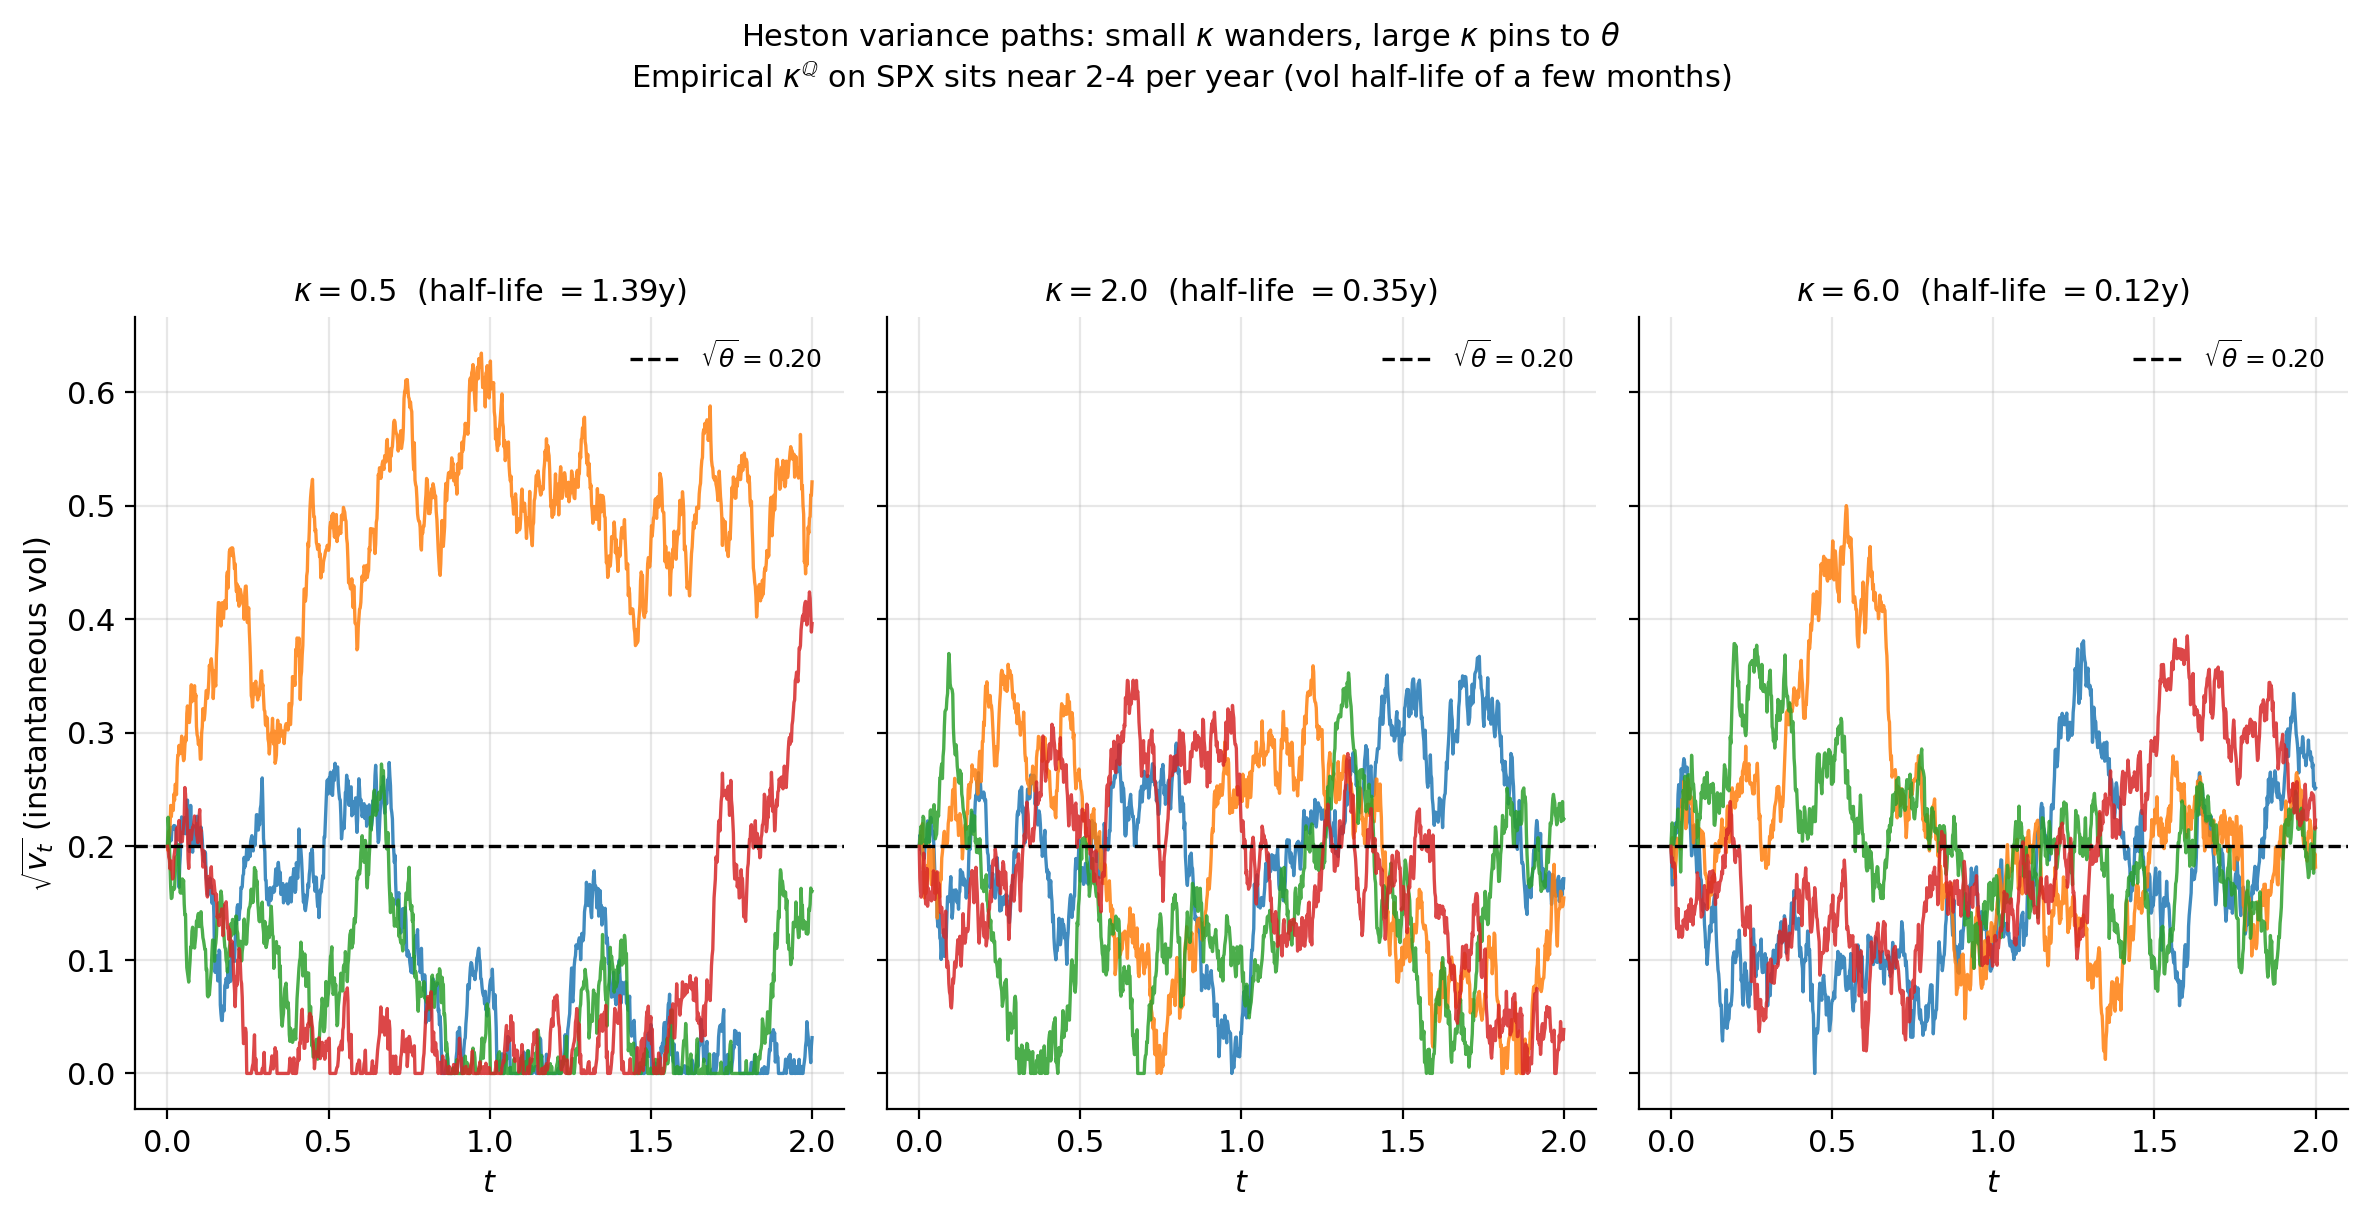
\includegraphics[keepaspectratio]{figures/ch10-variance-paths-kappa.png}}
\caption{CIR variance paths under three different \(\kappa\) values
(same \(\theta=0.04\)): small \(\kappa\) wanders, large \(\kappa\) pins
paths tightly to \(\sqrt{\theta}\). Empirical SPX
\(\kappa^{\mathbb{Q}}\) since 2010 sits near 2-4/year, giving vol-shock
half-lives of 2-4 months --- consistent with how a VIX spike from 30
back to 15 typically resolves over a quarter}
\end{figure}

\section{10.2 Feller condition}\label{feller-condition}

The variance process (10.7) can hit zero. For \(v_t\) to be strictly
positive (i.e.~to avoid hitting zero and getting stuck / reflecting) we
need \[
\boxed{\; 2\,\kappa^{\mathbb{P}}\,\theta^{\mathbb{P}} \;\ge\; \alpha^2 \;}
\tag{10.9}
\] the Feller condition. Intuition: \(2\kappa\theta\) is twice the pull
back toward the mean at the origin (the drift at \(v=0\) is
\(\kappa\theta\)), while \(\alpha^2\) is the diffusion push that drives
\(v\) around. When the pull dominates, the origin is an entrance-only
boundary and \(v_t\) is \(>0\) almost surely. When the push dominates,
\(v_t\) can touch zero (and in continuous time will, repeatedly). In
practice calibrated equity parameters often violate it mildly;
simulation schemes then use full-truncation (take \(v^+ = \max(v,0)\) in
the diffusion coefficient) or reflection. Closed-form pricing is
unaffected --- the characteristic function is analytic in the parameters
regardless of Feller.

\textbf{Boundary classification.} For the CIR variance, the origin is
\emph{inaccessible} --- Feller-classified as an entrance-natural
boundary in the strict-inequality case, sometimes loosely called
``entrance'' --- when \(2\kappa\theta \ge \alpha^2\), and \emph{regular}
(reachable, requires a boundary rule) otherwise. The stationary density
of \(v_t\) is gamma-distributed with shape \(2\kappa\theta/\alpha^2\)
--- bounded at the origin if Feller holds, divergent (but integrable)
like \(v^{2\kappa\theta/\alpha^2 - 1}\) if violated.

\textbf{Calibrated Heston typically violates Feller mildly.} The market
demands more wing richness than a Feller-compliant calibration can
deliver, so the calibrator cranks \(\alpha\) across the boundary.
Closed-form pricing is unaffected; Monte Carlo simulation needs careful
handling.

\textbf{Simulation hierarchy} (fastest/crudest to slowest/most
accurate):

\begin{enumerate}
\def\labelenumi{\arabic{enumi}.}
\tightlist
\item
  \textbf{Euler with full truncation} (Lord--Koekkoek--Van Dijk 2010):
  clamp \(v\) at zero in the diffusion coefficient.
  Linear-in-\(\Delta t\) bias; for daily steps the ATM bias is typically
  under 0.5\%.
\item
  \textbf{Quadratic-Exponential (QE)} (Andersen 2007): approximates the
  non-central chi-squared transition density by a quadratic-of-normal in
  the high regime and a normal-plus-point-mass in the low regime.
  2--3\(\times\) slower than Euler, \textasciitilde10\(\times\) more
  accurate. Production workhorse.
\item
  \textbf{Exact (Broadie--Kaya 2006):} draw directly from the
  non-central chi-squared transition. Zero bias but expensive; reserve
  for benchmarking.
\end{enumerate}

For vanillas, the Fourier closed form skips MC entirely.

\pandocbounded{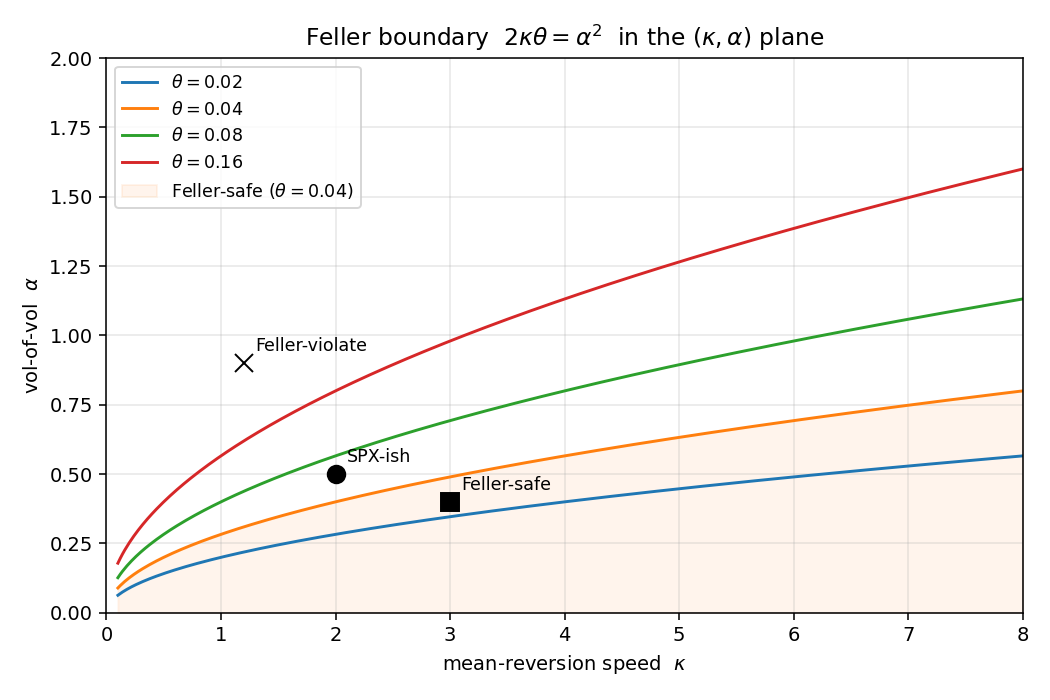
\includegraphics[keepaspectratio]{figures/ch10-heston-feller-boundary.png}}
\emph{Feller boundary \(\alpha = \sqrt{2\kappa\theta}\) for four
long-run variance levels. SPX-like calibrations sit slightly above --- a
textbook mild violation.}

\begin{figure}
\centering
\pandocbounded{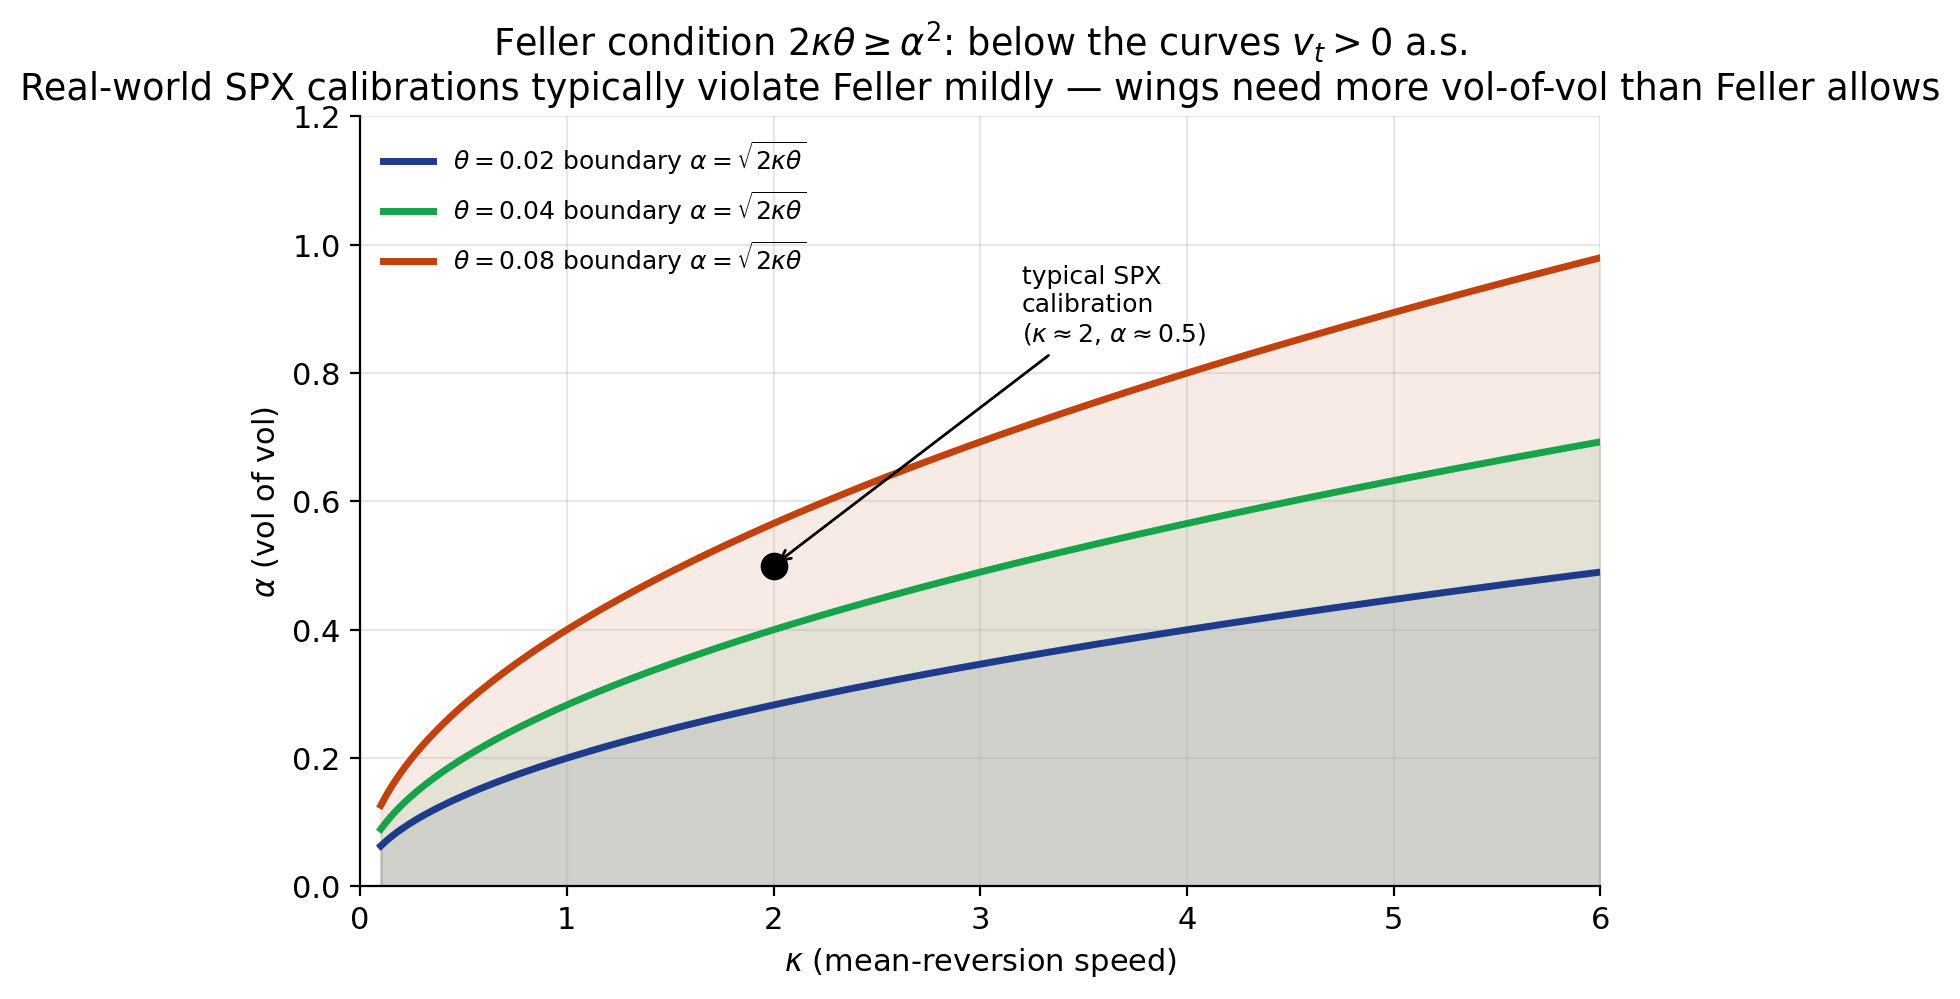
\includegraphics[keepaspectratio]{figures/ch10-feller-phase.png}}
\caption{Feller phase diagram with a typical SPX calibration point
(\(\kappa\approx 2\), \(\alpha\approx 0.5\)) annotated. The point sits
\emph{above} the \(\theta=0.04\) boundary --- i.e.~Feller is mildly
violated, exactly as quant-vol desks routinely observe in calibrated
production parameters}
\end{figure}

\begin{center}\rule{0.5\linewidth}{0.5pt}\end{center}

\section{10.3 Change of measure --- market price of variance
risk}\label{change-of-measure-market-price-of-variance-risk}

Going from \(\mathbb{P}\) to \(\mathbb{Q}\), (10.6) loses its drift
(futures are martingales), \[
\frac{\mathrm{d}F_t}{F_t} = \sqrt{v_t}\,\mathrm{d}W_t^{F},
\qquad \text{corr.\ }(\rho).
\tag{10.10}
\] For the variance, write the Girsanov shift --- the multi-dimensional
version derived in Chapter 5 §5.4, specialised here to two correlated
Brownian motions: \[
\mathrm{d}W_t^{F} = \frac{\mu_t}{\sqrt{v_t}}\,\mathrm{d}t + \mathrm{d}W_t^{\mathbb{P},F},
\qquad
\mathrm{d}W_t^{v} = \lambda_t^{v}\,\mathrm{d}t + \mathrm{d}W_t^{\mathbb{P},v}.
\tag{10.11}
\] Then the \(\mathbb{Q}\)-dynamics of variance become \[
\mathrm{d}v_t = \Big(\kappa^{\mathbb{P}}(\theta^{\mathbb{P}} - v_t) \;-\; \alpha\,\lambda_t^{v}\sqrt{v_t}\Big)\mathrm{d}t \;+\; \alpha\sqrt{v_t}\,\mathrm{d}W_t^{v},
\tag{10.12}
\] with \(\lambda_t^{v}\) the market price of variance (vol) risk. The
two-dimensional Girsanov we are using is the vector-valued version: we
apply independent density processes to two correlated Brownian motions
by first rotating into an independent pair via Cholesky, shifting each,
and rotating back. The net effect on the correlated pair \((W^F, W^v)\)
is recorded in (10.11); the correlation \(\rho\) is preserved by the
change of measure, as the Girsanov shift is a pure drift adjustment and
does not affect the quadratic covariation.

Here is the crucial point. The drift of variance under \(\mathbb{P}\) is
whatever we think it is empirically --- it reflects the long-run mean of
realised variance, the speed at which variance reverts after shocks, and
so on. But for option pricing, we do not price under \(\mathbb{P}\); we
price under \(\mathbb{Q}\). And \(\mathbb{Q}\) attaches a different
drift to the variance process, because market participants demand (or
offer) a premium for bearing variance risk. Empirically, buyers of
variance --- people long volatility through options or variance swaps
--- pay a premium on average, meaning realised variance comes in lower
than implied variance on average. This is the variance risk premium, and
it is captured in the model by \(\lambda^v\). A negative \(\lambda^v\)
for equity markets would reflect the fact that long-vol positions earn a
negative premium --- they are hedges, and hedges cost something. The
variance risk premium is persistent, documented over long samples, and
is arguably the single most important empirical feature driving the
wedge between historical and implied vol.

To put numbers on this: over long samples of SPX options, the average
difference between implied variance (VIX\(^2\)-scaled) and subsequently
realised variance is about 3--5 percentage points in annualised-vol
units. In other words, if VIX is 20, realised vol over the next 30 days
averages about 17. Variance-swap investors --- the sellers of variance
--- earn this 3--5 point wedge on average, net of trading costs, and
this is the explicit compensation for bearing tail-risk exposure. (The
wedge is not risk-free, obviously; it can invert during crises, and the
shorts can take large losses. Long-vol positions are attractive when vol
spikes, which is exactly the ``tail hedge'' use case that dominates
quant-institutional flows.) When we write Heston with a specific
\(\lambda^v\), we are implicitly asserting a particular functional form
for this premium --- one that is compatible with the CIR dynamics.
Different asset classes and different regimes have different premium
structures; Heston's affine-preserving choices capture the main cases
cleanly.

A pedagogical note on terminology. The ``market price of variance risk''
is sometimes written \(\lambda^v\) and sometimes with other symbols; the
economic quantity it represents is the Sharpe-ratio-like premium
demanded per unit of variance-factor exposure. If the variance risk is
priced (i.e.~\(\lambda^v \ne 0\)), then the \(\mathbb{Q}\)- dynamics of
\(v\) differ from the \(\mathbb{P}\)-dynamics, which means the
risk-neutral expected path of variance differs from the physical
expected path. Practitioners often summarise this by saying ``implied
vol is higher than expected realised vol on average, by the variance
risk premium.'' That one sentence captures essentially the entire
economics of the \(\lambda^v\) parameter.

Two natural choices keep the SDE affine (preserving Heston form):

\textbf{Choice 1.} \(\lambda_t^{v} = c\sqrt{v_t}\). Then \[
\lambda_t^{v}\cdot\alpha\sqrt{v_t} = \alpha c\,v_t,
\] so the drift becomes \[
\kappa^{\mathbb{P}}\theta^{\mathbb{P}} - (\kappa^{\mathbb{P}} + \alpha c)\,v_t
= \kappa\!\left(\frac{\kappa^{\mathbb{P}}\theta^{\mathbb{P}}}{\kappa} - v_t\right),
\tag{10.13}
\] with \(\kappa = \kappa^{\mathbb{P}} + \alpha c\) and
\(\theta = \kappa^{\mathbb{P}}\theta^{\mathbb{P}}/\kappa\).

\textbf{Choice 2.}
\(\lambda_t^{v} = \dfrac{\ell}{\sqrt{v_t}} + c\sqrt{v_t}\). Then \[
\lambda_t^{v}\cdot\alpha\sqrt{v_t} = \alpha\ell + \alpha c\,v_t,
\] so both level and slope of the mean-reversion shift:
\(\kappa = \kappa^{\mathbb{P}} + \alpha c\) and
\(\theta = (\kappa^{\mathbb{P}}\theta^{\mathbb{P}} - \alpha\ell)/\kappa\).

Notice what (10.13) achieves: the shape of the variance SDE under
\(\mathbb{Q}\) is algebraically identical to its shape under
\(\mathbb{P}\) --- the same
\(\kappa(\theta - v)\,\mathrm{d}t + \alpha\sqrt{v}\,\mathrm{d}W\) form
--- with \((\kappa, \theta)\) reshuffled. This is why Heston is so
clean. A wrong choice of \(\lambda^v\) (say, a constant \(\lambda\))
would break the affine structure: the change of measure would contribute
\(\alpha\lambda\sqrt{v}\) to the drift, which is not linear in \(v\),
and the Riccati tractability would collapse. The two
``affine-preserving'' choices above are the ones that respect Heston's
algebraic skeleton, and they cover the usual practitioner
parametrisations.

This is a subtle but deep point. In most finance contexts, the choice of
\(\lambda^v\) is driven by economic or statistical arguments: we want
the risk-neutral measure that best fits observed data, or that has some
desired theoretical property. In Heston, there is an additional
computational constraint: only certain functional forms of \(\lambda^v\)
preserve the affine structure, and only affine structure gives us the
closed-form characteristic function. If we chose a \(\lambda^v\) that
broke affine-ness, the Riccati ODEs would become general nonlinear ODEs
(without closed form), the characteristic function would require
numerical PDE solving at every evaluation, and the computational cost of
Heston pricing would increase by two or three orders of magnitude. For
this reason, the affine-preserving \(\lambda^v\) choices are not just
theoretically elegant --- they are computationally essential. They are
the reason we can calibrate Heston to a full vol surface in seconds
rather than hours.

Another way to see this: the ``Heston model under \(\mathbb{Q}\)'' and
the ``Heston model under \(\mathbb{P}\)'' are two instances of the same
algebraic family, parameterised differently. Pricing derivatives uses
the \(\mathbb{Q}\)-instance; estimating historical dynamics uses the
\(\mathbb{P}\)-instance; the affine-preserving change-of-measure
provides the bridge between them. If you wanted to do joint estimation
--- fitting both physical time-series data and risk-neutral option data
simultaneously --- you would use this bridge to write down the joint
likelihood, with \(\lambda^v\) as the parameter linking the two. Some
sophisticated calibration frameworks do exactly this, treating the
variance risk premium as a directly estimable parameter. Most
practitioner implementations, however, calibrate under \(\mathbb{Q}\)
only and infer the risk premium ex post by comparing calibrated
parameters to historical estimates.

From the option trader's perspective, this means something striking. The
risk-neutral \((\kappa, \theta, \alpha, \rho, v_0)\) that we calibrate
from option prices are not the same as the physical-measure
\((\kappa^{\mathbb{P}}, \theta^{\mathbb{P}}, \alpha^{\mathbb{P}},
\rho^{\mathbb{P}}, v_0^{\mathbb{P}})\) that we might estimate from
historical returns. The two sets of parameters differ precisely by
\(\lambda^v\), the variance risk premium. Typically
\(\theta > \theta^{\mathbb{P}}\) --- the risk-neutral long-run variance
is higher than the historical long-run variance --- because buyers of
variance swaps must be compensated. The gap is the variance risk premium
in disguise, and it is paid for by the option buyer and collected by the
option seller.

The implications for trading are concrete. A strategy of systematically
selling variance (selling options, selling variance swaps, running a
``vol carry'' book) earns the premium on average but takes on
significant tail risk: in a vol spike the P\&L can be punishingly
negative. The Sharpe ratio of such a strategy is positive but not
spectacular --- typically in the range 0.5 to 1.0 for liquid markets
over long samples --- and the drawdowns are deep. LTCM's 1998 blowup,
the 2018 ``Volmageddon'' that wiped out XIV, and the March 2020 vol
spike are all examples of this strategy's tail risk materialising.
Understanding the origin of the premium via Heston's \(\lambda^v\) helps
demystify the strategy: the premium is compensation for exactly the tail
exposure that occasionally bites hard. There is no free lunch; just a
structural risk-premium for those willing to bear the risk.

It is also worth noting that the risk-neutral \(\alpha\) can differ from
the physical \(\alpha^{\mathbb{P}}\), and the risk-neutral \(\rho\) can
differ from \(\rho^{\mathbb{P}}\), depending on the precise form of
\(\lambda^v\) (and on whether there is a price of correlation-risk in
addition to vol-risk). In the simplest affine-preserving choice (Choice
1 above), \(\alpha\) and \(\rho\) are preserved across measures; only
\(\kappa\) and \(\theta\) shift. In richer parameterisations, all four
can shift. Practitioners usually take the simplest case and then check
empirically whether the calibrated \(\alpha\) and \(\rho\) are
consistent with time-series estimates. Significant discrepancies suggest
either model misspecification or a richer risk-premium structure than
the simple model captures.

Under \(\mathbb{Q}\) (market price of risk absorbed, with Heston's
canonical choice), we get the standard Heston system: \[
\boxed{\;
\frac{\mathrm{d}F_t}{F_t} = \sqrt{v_t}\,\mathrm{d}W_t^{F}
\;}
\tag{10.14}
\] \[
\boxed{\;
\mathrm{d}v_t = \kappa(\theta - v_t)\,\mathrm{d}t + \alpha\sqrt{v_t}\,\mathrm{d}W_t^{v}
\;}
\tag{10.15}
\] with \(\mathrm{d}W_t^{F}\cdot\mathrm{d}W_t^{v} = \rho\,\mathrm{d}t\).

\begin{quote}
From here on, \((\kappa, \theta, \alpha, \rho, v_0)\) are the five
risk-neutral Heston parameters.
\end{quote}

Five parameters is a modest parameter count for a model that fits an
entire implied vol surface. By comparison, some practitioner ``local
vol'' or ``local-stochastic vol'' models carry dozens or even hundreds
of parameters. The minimalism of Heston is one of its virtues: each
parameter has a clean economic meaning, calibration is a well-posed
optimisation in low dimension, and the fitted parameters can be compared
across dates and assets without the apples-to-oranges problem that
plagues over-parameterised models.

The parsimony has a second benefit that is sometimes overlooked:
generalisation. A five-parameter model fitted to (say) ATM vols and the
25-delta risk reversal and the 25-delta butterfly at a single maturity
has four effective calibration targets and five parameters, so the fit
is nearly exact. But those same five parameters then extrapolate --- via
the Heston dynamics --- to every other strike and every other maturity.
The extrapolation is not arbitrary; it is dictated by the structural
form of the Heston SDE. This means the model can price exotic and
off-the-grid strikes in a way that is internally consistent with the
calibration points, and that is one of the reasons Heston is a favourite
choice for pricing mildly exotic products like barriers, forward-starts,
and cliquets. A dense local-vol model with hundreds of parameters can
fit the grid exactly, but extrapolates poorly off the grid because there
are no dynamics constraining what happens between quoted points. Heston,
with five parameters, is forced to make structural assumptions that
constrain the extrapolation --- often to the benefit of the exotic
pricing.

Compare this to regime-switching models, which can have many parameters
per regime (shape of transition matrix, regime-specific vols,
regime-specific jump intensities) and easily bloat to 15+ parameters.
Those models offer richer dynamics but are less stable across
calibrations and harder to interpret. Heston's five-parameter structure
sits in the sweet spot: rich enough to capture the major features of vol
dynamics (mean reversion, vol-of-vol, leverage), parsimonious enough to
calibrate cleanly and be interpreted economically. This sweet spot is a
big part of why Heston has endured as the industry default.

\begin{center}\rule{0.5\linewidth}{0.5pt}\end{center}

\section{10.4 Implied volatility --- why we need this
model}\label{implied-volatility-why-we-need-this-model}

If we price a call in the Heston world at \((K,T)\) and invert
Black--Scholes to back out the volatility that matches, we get the
implied vol surface: \[
V^{\text{Heston}}(K,T) \;=\; V^{\text{BS}}\!\big(r,\,\sigma^{\text{impvol}}(K,T);\, K, T\big).
\tag{10.16}
\] The Heston model produces a volatility smile in \(K\) and a
non-trivial term structure in \(T\). Graphically: out-of-the-money puts
(low \(K\)) and calls (high \(K\)) price richer than BS, bending the
flat BS line into a smile/skew. The PDF of \(\ln X_T\) under Heston is
fatter-tailed and skewed relative to the BS log-normal. Payoff
\((X-K)_+\) is sensitive to those tails.

\textbf{Implied vol as coordinate chart.} Implied vol is a BS-formula
bijection between price and a ``vol unit''; the BS formula here is a
quoting convention, not a pricing model. The Heston density of
\(\ln F_T\) is a continuous mixture of lognormals indexed by the
integrated variance \(I_T = \int_0^T v_s\,\mathrm{d}s\). Mixing fattens
the tails (kurtosis
\(\approx 3 + 6\,\mathrm{Var}(I_T)/\mathbb{E}[I_T]^2\)), and \(\alpha\)
drives the wings.

\textbf{Skew from \(\rho\).} With \(\rho < 0\), low-\(F_T\) scenarios
are precisely the ones with high integrated variance --- the mixture
asymmetrises, the left tail fattens, the right tail thins. The smile
evolves from symmetric (at \(\rho = 0\)) through equity-style skew
(\(\rho = -0.7\)) to a pure downward line as \(\rho \to -1\). The
characteristic-function framework handles all of this implicitly without
needing to write down the mixture explicitly.

\pandocbounded{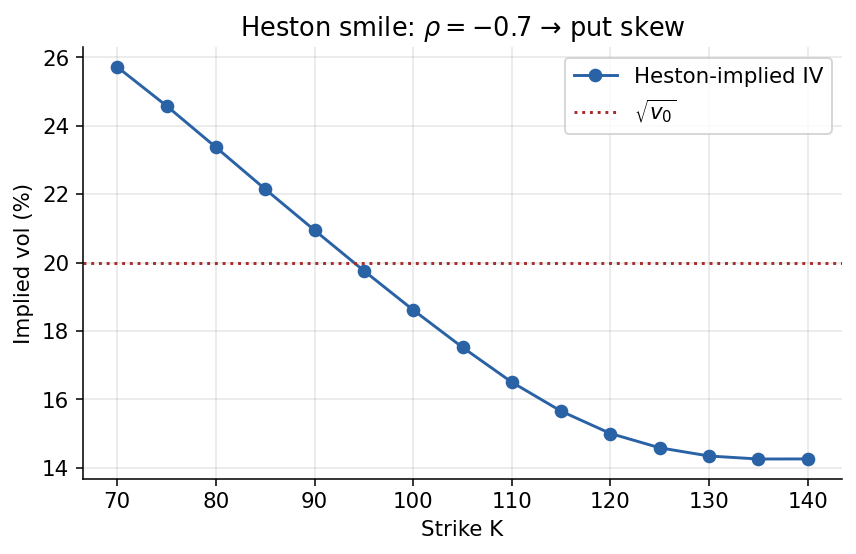
\includegraphics[keepaspectratio]{figures/ch10-heston-smile.png}}
\emph{Heston-implied IV smile}

\begin{figure}
\centering
\pandocbounded{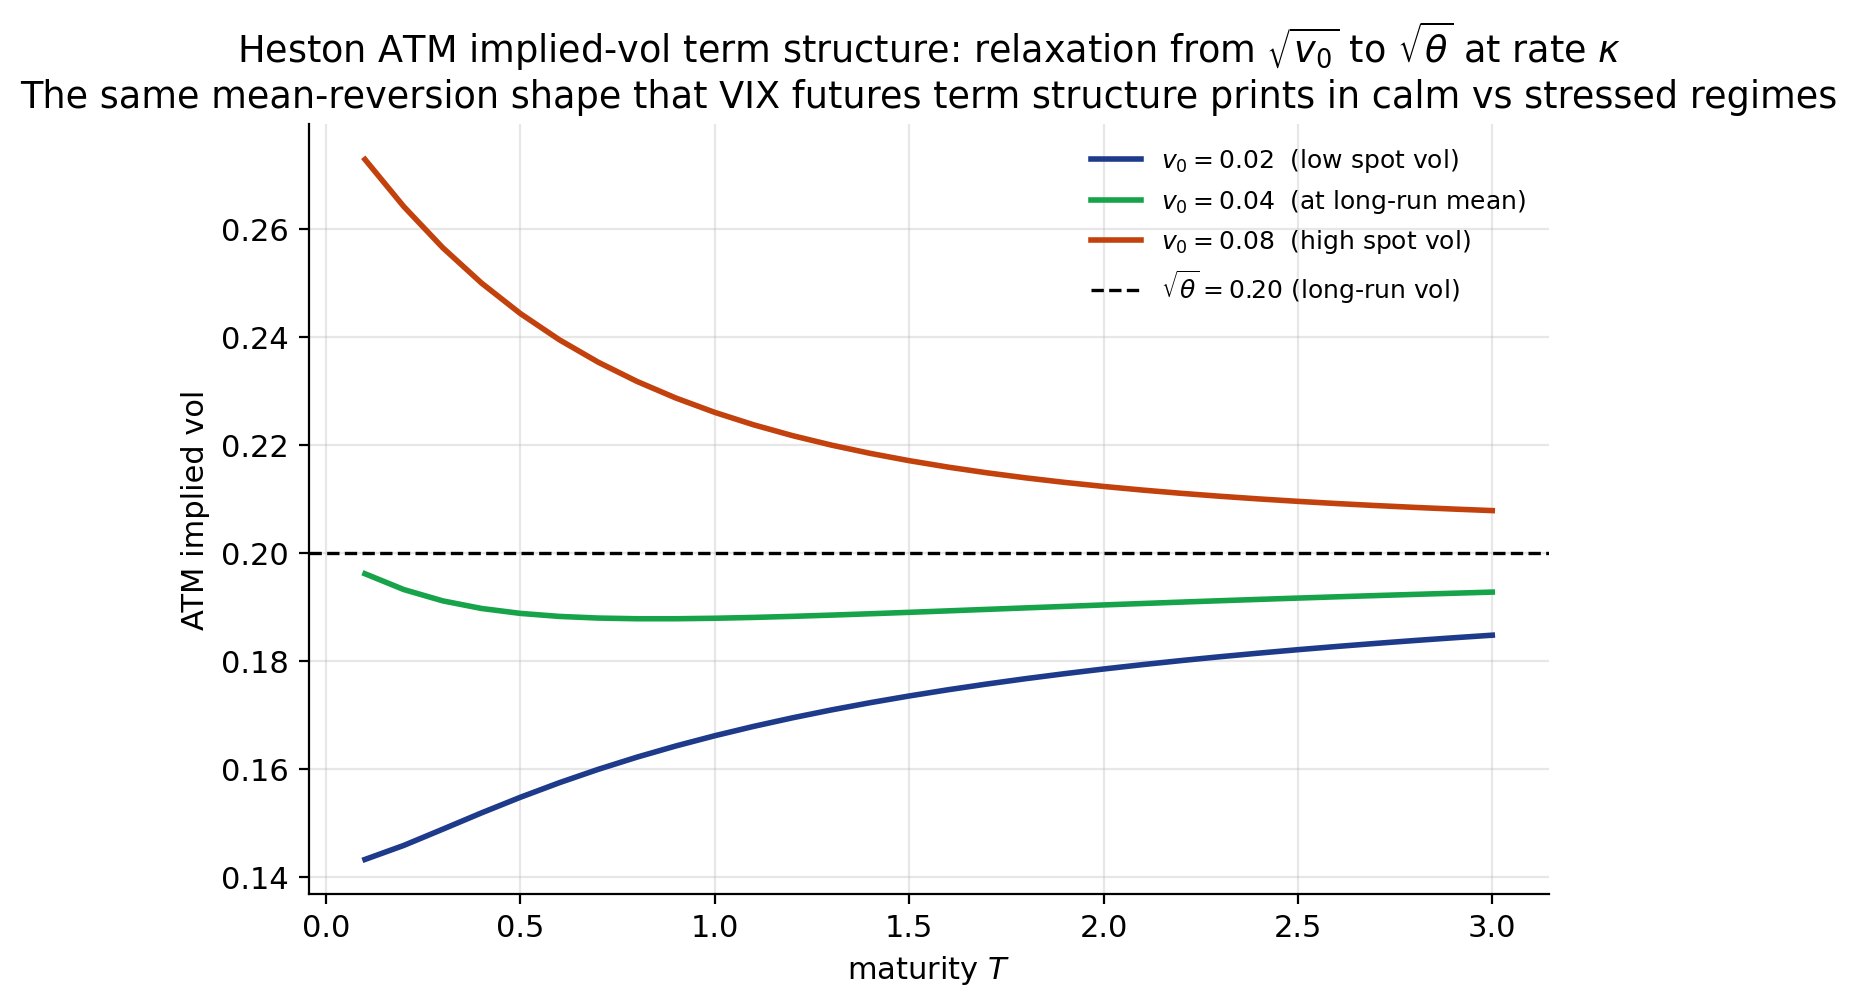
\includegraphics[keepaspectratio]{figures/ch10-atm-term-structure.png}}
\caption{Heston ATM implied vol vs maturity for three spot-variance
starts: convergence to \(\sqrt{\theta}\) as \(T\to\infty\) at rate
\(\kappa\). Same mean-reversion that VIX-futures term structure prints
--- short-end contango in calm, backwardation when spot vol spikes above
the long-run level}
\end{figure}

\subsection{Case study (a): 1987 crash and the birth of vol
skew}\label{case-study-a-1987-crash-and-the-birth-of-vol-skew}

\emph{Pre-1987 BS-implied vols were essentially flat across strikes.}
\emph{Post-Oct 1987 the equity-index left skew became a permanent
fixture.} \emph{Heston with \(\rho < 0\) is the simplest model that
reproduces it.}

\textbf{Context.} Through the 1970s and early 1980s, Black-Scholes
flat-vol calibrations produced implied vols that were, for liquid index
options, roughly flat across strikes --- the small differences (a
``smile'' with slight bowing toward OTM strikes) were treated as a
numerical curiosity arising from BS's lognormal misspecification. On 19
October 1987 the S\&P 500 fell 20.5\% in a single session; the SPX
OEX-style listed put options that traded the following day repriced at
radically different implied vols across strikes, with the deepest OTM
puts trading at vols 5--10 points above ATM. Over the months following,
the ``skew'' persisted at every observation; by 1990 it had become a
permanent structural feature of equity index option pricing, distinct
from the modest smile visible in single-stock or commodity option
markets.

Mark Rubinstein's ``Implied Binomial Trees'' (Journal of Finance, 1994)
is the canonical academic documentation of the post-1987 skew: he
constructed binomial trees fitted to S\&P 500 option quotes pre- and
post-crash and showed the implied risk-neutral density of \(\ln S_T\)
shifted from the symmetric-fattened-tails of pre-1987 to a strongly
left-skewed distribution post-1987. Subsequent work by Bates (1996),
Bakshi-Cao-Chen (1997), and others quantified the skew's persistence
across decades and across markets --- wherever a 1987-style large
downward move had occurred (or was perceived as possible), the permanent
skew followed.

\textbf{Through the chapter's math.} Black-Scholes lognormality (Chapter
6, equation 6.12) imposes a \emph{symmetric} distribution on \(\ln S_T\)
--- the left and right tails have identical shape. To produce a skew,
you must either (i) introduce jumps (Merton 1976, Bates 1996), or (ii)
make volatility itself stochastic with a non-zero spot-vol correlation.
The Heston specification (10.1) does the second: the variance process
\(v_t\) is correlated \(\rho\) with the spot innovation, and with
\(\rho < 0\) the joint distribution skews exactly as the empirical
post-1987 surface demands. The mechanism is captured by the mixture
decomposition above: under \(\rho < 0\), paths with low terminal \(F_T\)
tend to have \emph{high} integrated variance
\(I_T = \int v_s\,\mathrm ds\) (vol spiked as the spot crashed), so the
conditional density of \(\ln F_T\) given low \(F_T\) is fat-tailed ---
exactly what makes OTM puts richer than BS quotes. A typical 2025 SPX
surface fits to \(\rho \in [-0.80, -0.60]\) --- that number is not a
free parameter, it is the market's price of structural joint crash risk
inherited from October 1987.

\textbf{Lesson.} The skew is not a model defect to be calibrated away
--- it is the market's \emph{structural memory} of asymmetric tail risk.
Every flat-vol BS calibration since 1987 has been systematically wrong
on OTM puts (it under-prices them) and wrong on OTM calls (it
over-prices them, slightly). The empirical case for stochastic
volatility, and specifically for \(\rho < 0\) in the Heston framework,
is exactly the post-1987 fact that no symmetric model can reproduce a
persistent left skew. Practitioners read \(\rho\) as a ``leverage
parameter'' --- the more leveraged the underlying (equity indices in
markets where firms carry debt), the more negative \(\rho\) tends to be.
Fixed-income, FX, and commodity surfaces exhibit much smaller (or zero)
skew because their underlying processes do not have the same structural
joint-crash dynamic. The lesson for this chapter is that \(\rho\) is not
a fudge factor; it is the most information-dense parameter in the
calibration, and a desk that locks \(\rho\) at a stale value is hedging
a fundamentally different surface than the market is quoting.

\begin{center}\rule{0.5\linewidth}{0.5pt}\end{center}

\subsection{10.4.1 Simulation scheme}\label{simulation-scheme}

Set \(X_t = \ln F_t\). Itô (two-dimensional, Chapter 3 §3.10) gives \[
\mathrm{d}X_t = -\tfrac{1}{2}\,\gamma^2 v_t\,\mathrm{d}t + \gamma\sqrt{v_t}\,\mathrm{d}W_t^{F},
\tag{10.17}
\] (with \(\gamma = 1\) for the pure Heston; we keep \(\gamma\) to track
units). Euler-discretise with step \(\Delta t\): \[
X_{t_n} - X_{t_{n-1}} = -\tfrac{1}{2}\gamma^2 v_{t_{n-1}}^{+}\,\Delta t + \gamma\sqrt{v_{t_{n-1}}^{+}}\,\sqrt{\Delta t}\,Z_{1,n},
\tag{10.18}
\] \[
v_{t_n} - v_{t_{n-1}} = \kappa(\theta - v_{t_{n-1}}^{+})\,\Delta t + \alpha\sqrt{v_{t_{n-1}}^{+}}\,\sqrt{\Delta t}\left(\rho\,Z_{1,n} + \sqrt{1-\rho^2}\,Z_{2,n}\right),
\tag{10.19}
\] where \(Z_{1,n}, Z_{2,n}\) are i.i.d.~\(\mathcal{N}(0,1)\) and \[
v_t^{+} \;=\; \max(v_t,\,0)
\tag{10.20}
\] is the full-truncation fix (Lord--Koekkoek--Van Dijk) that prevents
\(\sqrt{v}\) from going complex when Feller is violated.

The scheme as written has a number of subtle features worth
appreciating. The two innovations \(Z_1, Z_2\) are independent standard
normals; the linear combination \(\rho Z_1 + \sqrt{1 - \rho^2}\,Z_2\)
produces a normal with variance one that is correlated \(\rho\) with
\(Z_1\). This is the standard trick for sampling from a bivariate normal
by Cholesky factorisation. The use of \(v^+\) in both the drift and the
diffusion of the variance update ensures that even if a previous step
dragged \(v\) below zero, we do not propagate that negativity: the next
step treats \(v\) as if it were zero, allowing the mean-reversion drift
\(\kappa\theta\) to lift it back into positive territory at the next
time step. Full truncation is biased --- it systematically
underestimates the variance of \(v\) near zero --- but the bias shrinks
as \(\Delta t \to 0\) and is widely accepted as the best trade-off
between simplicity and accuracy for standard use cases.

A practical note on step size. For daily-step Heston simulation
(\(\Delta t = 1/252\)), the full-truncation Euler scheme introduces bias
on European option prices of a few basis points typically --- perfectly
acceptable for most risk-management purposes. For path-dependent options
(barriers, Asians, forward-starts), the bias can be larger, and finer
time steps or better schemes (QE) become necessary. For very short-dated
options (days or less), \(\Delta t = 1/(252 \cdot N)\) with \(N\) in the
range 10--100 intraday sub-steps is often needed. The computational cost
scales linearly with the number of steps, so the choice of \(N\) is a
cost-accuracy tradeoff that should be benchmarked against the
closed-form Heston price before committing to a production scheme.

A related practical note: use antithetic variates to reduce MC variance.
Heston's dynamics are symmetric in \((Z_1, Z_2) \to (-Z_1, -Z_2)\) ---
flipping the signs of both innovations produces an equally probable
path. Pricing the option on both the original and the flipped path and
averaging the two gives a zero-bias variance reduction that typically
cuts MC standard error by a factor of 1.5--2\(\times\) at no extra
computational cost (since the variance update for the flipped path is
essentially free). This and other variance-reduction techniques (control
variates based on the BS or Heston closed-form price, importance
sampling) are standard tools developed in Chapter 9 and routinely used
in production vol desks.

Yet another subtle but important consideration is the discretisation of
the spot-variance coupling. In the Euler scheme as written, the spot
update uses \(v_{t_{n-1}}^+\) --- the variance at the start of the
interval --- as the diffusion coefficient. A more accurate scheme would
average the variance over the interval, e.g.\\
\((v_{t_{n-1}}^+ + v_{t_n}^+)/2\), but doing so introduces an implicit
coupling that requires iteration. Andersen's QE scheme handles this
coupling more carefully; naive Euler does not. The result is a small
bias in the joint spot-variance distribution that most implementations
accept as the cost of simplicity.

\pandocbounded{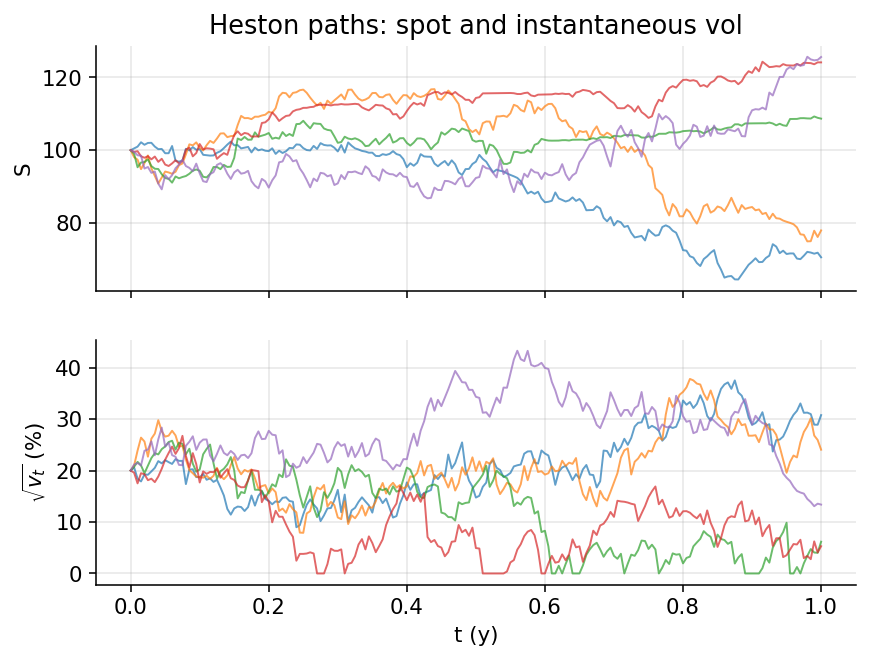
\includegraphics[keepaspectratio]{figures/ch10-heston-paths.png}}
\emph{Heston sample paths (S and sqrt(v))}

The figure shows two kinds of dynamics happening simultaneously. The top
panel traces the spot price, which looks at first glance like a standard
diffusion: it wanders, drifts, has typical diffusion jaggedness. But the
local volatility of that wander is not constant --- compare periods
where spot is oscillating gently with periods where it swings wildly.
The bottom panel shows the source of that varying agitation: it plots
\(\sqrt{v_t}\), the instantaneous volatility. Periods where
\(\sqrt{v_t}\) spikes correspond to the rough episodes on the spot
panel; periods where \(\sqrt{v_t}\) is low produce the calm stretches
above. Notice also the anticorrelation: when spot drops sharply,
\(\sqrt{v_t}\) tends to spike up, visible as the mirror-image texture
between the two panels. This is exactly what \(\rho < 0\) encodes, and
it is the microstructural fingerprint of equity markets.

Look, too, at the mean-reversion visible in the bottom panel. The
\(\sqrt{v_t}\) trace is not a random walk --- it oscillates around a
roughly horizontal baseline (the square root of \(\theta\)), with upward
spikes that decay back toward baseline over a few months. This is the
\(\kappa\)-rate relaxation in action. A random walk in \(\sqrt{v}\)
would drift further and further from any baseline; Heston's
mean-reverting variance creates a ``homing'' tendency that keeps the
long-run distribution bounded. Without mean reversion, the integrated
variance \(\int_0^T v\,\mathrm{d}s\) would grow too variable at long
horizons, and long-dated option pricing would become unstable. Mean
reversion is the mathematical device that keeps Heston well-behaved at
all horizons.

A subtle but important visual feature is the asymmetry of vol dynamics.
Real markets (and Heston with \(\rho < 0\)) exhibit ``sharp spikes up,
slow decays down'' in vol --- vol rises quickly during panics, falls
gradually as calm returns. This is not a property of the CIR process by
itself, which is symmetric in its innovation structure; it is a property
of the joint \((F, v)\) dynamics. When spot crashes, the coupled vol
spike happens all at once; when spot drifts sideways, vol decays at the
leisurely rate \(\kappa\). The resulting asymmetry in the vol trace is a
visible signature of \(\rho < 0\), and it matches the empirical
behaviour of VIX quite closely.

\begin{center}\rule{0.5\linewidth}{0.5pt}\end{center}

\section{10.5 Characteristic function via Riccati
ODEs}\label{characteristic-function-via-riccati-odes}

Define the conditional characteristic function of \(X_T = \ln F_T\): \[
g_t \;\equiv\; \mathbb{E}_t^{\mathbb{Q}}\!\left[\,e^{\omega(X_T - K)}\,\right] \;=\; g(t, X_t, v_t),
\tag{10.21}
\] for \(\omega \in \mathbb{C}\) on some admissible strip. (Setting
\(\omega = i\phi\) gives the usual Fourier transform in \(X_T\).) We
seek a PDE for \(g\) and then an exponential-affine ansatz.

Here is why we bother with the characteristic function at all. The
density \(p(X_T)\) of the log-futures price under Heston does not have a
closed form. It is a mixture of lognormals, indexed by the unobserved
path of variance, and the mixture weights are themselves complicated. We
have no hope of writing \(p\) down. The characteristic function, on the
other hand, turns out to be elementary --- a neat exponential-affine
expression in the state --- and it contains exactly the same information
as the density. Every moment of the distribution can be read off from
derivatives of the characteristic function at zero; every expectation of
the form \(\mathbb{E}[f(X_T)]\) can be computed by Fourier inversion,
provided \(f\) has a well-defined Fourier transform. European option
prices are linear functionals of the density, so the Fourier route is
not only convenient --- it is the natural one.

\begin{figure}
\centering
\pandocbounded{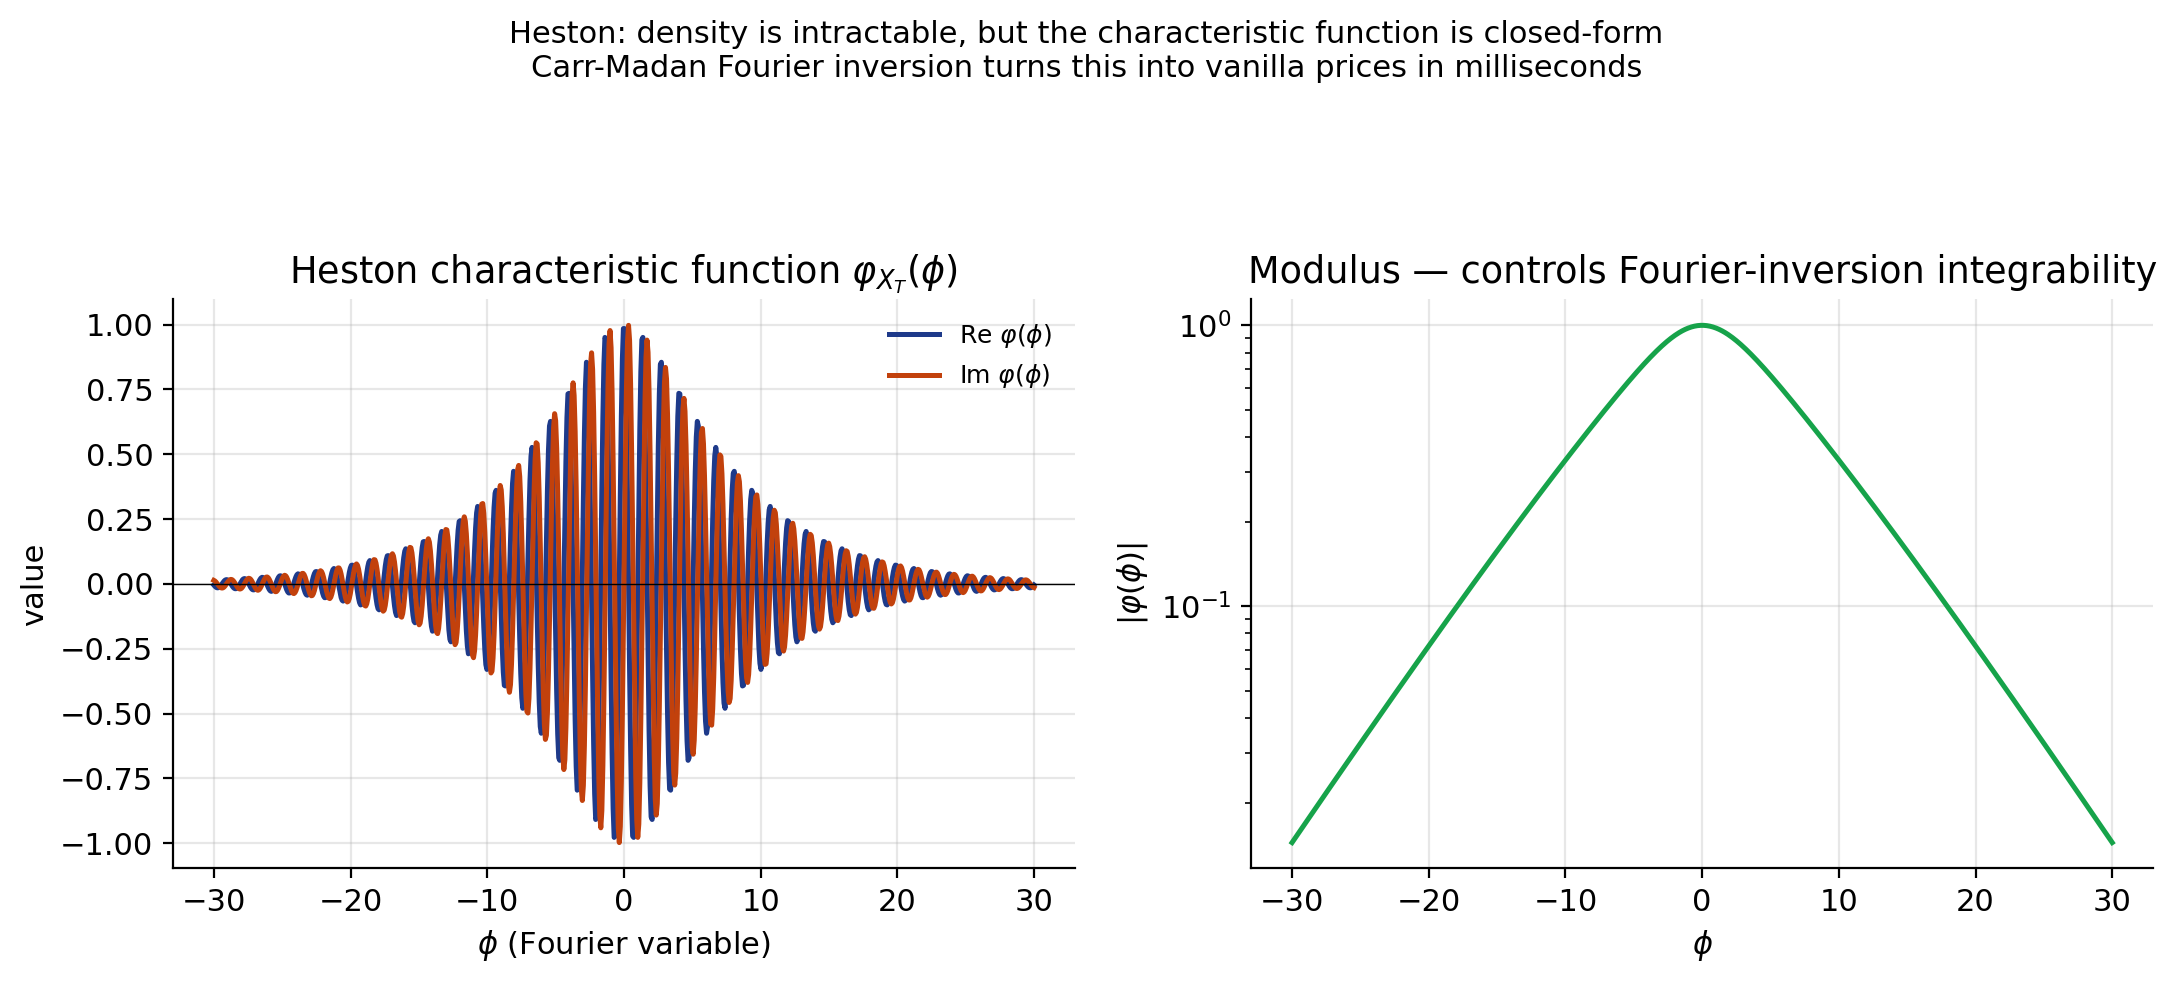
\includegraphics[keepaspectratio]{figures/ch10-charfunc-realimag.png}}
\caption{Real and imaginary parts of the Heston characteristic function
\(\varphi_{X_T}(\phi)\) alongside its modulus (right) at \(T=1\). The
density of \(\log S_T\) is hopeless to write down; this is the
closed-form replacement that Carr-Madan FFT inverts to produce vanilla
prices in milliseconds for every \((K, T)\) on a vol-surface grid}
\end{figure}

The philosophical shift from density-first to
characteristic-function-first thinking is one of the most important
reorientations in modern derivatives pricing. Classical probability
texts teach you to work with densities because densities are concrete
--- you can plot them, integrate against them, compute moments by direct
integration. But densities for complicated processes are often
impossible to write down in closed form, while characteristic functions
for the same processes are often much simpler. This is not an accident;
it reflects the fact that taking exponential expectations of
Gaussian-linked processes produces relatively clean algebra, while
writing down the density requires inverting that exponential expectation
via Fourier inversion --- which is a separate operation that may or may
not yield a closed-form answer. For many practical problems, you do not
need the density at all; you just need some expectation, and the
characteristic function gets you there directly via Fourier inversion or
via moment formulas.

Another way to see why characteristic functions are natural here: they
are the multiplicative objects of probability theory. When you add two
independent random variables, their densities convolve --- a
multiplicative operation in the characteristic-function domain via the
inverse Fourier relation. When you scale or shift, the characteristic
function transforms by simple algebraic operations. For stochastic
processes that are linear combinations of independent increments, the
characteristic function structure is essentially combinatorial. Heston's
integrated variance is such a construction, and its characteristic
function reflects this combinatorial structure cleanly.

\subsection{\texorpdfstring{10.5.1 Itô PDE for
\(g\)}{10.5.1 Itô PDE for g}}\label{ituxf4-pde-for-g}

Applying two-dimensional Itô to \(g(t, X_t, v_t)\) (Chapter 3 §3.10):
the bivariate SDE under \(\mathbb{Q}\) is (10.17) + (10.15) with
\(\mathrm{d}X \cdot \mathrm{d}v = \rho\,\alpha\,v_t\,\mathrm{d}t\). Then
\[
\mathrm{d}g_t = \partial_t g\,\mathrm{d}t + \partial_x g\,\mathrm{d}X_t + \partial_v g\,\mathrm{d}v_t
+ \tfrac{1}{2}\partial_{xx} g\,(\mathrm{d}X_t)^2
+ \tfrac{1}{2}\partial_{vv} g\,(\mathrm{d}v_t)^2
+ \partial_{xv} g\,(\mathrm{d}X_t\,\mathrm{d}v_t).
\tag{10.22}
\] Substituting the drifts and quadratic variations
\((\mathrm{d}X)^2 = v\,\mathrm{d}t\),
\((\mathrm{d}v)^2 = \alpha^2 v\,\mathrm{d}t\),
\(\mathrm{d}X\,\mathrm{d}v = \rho\alpha v\,\mathrm{d}t\), \[
\mathrm{d}g_t = \mathrm{d}t\left\{\partial_t g + \left(-\tfrac{1}{2}\gamma^2 v_t\right)\partial_x g + \kappa(\theta - v_t)\,\partial_v g
+ \tfrac{1}{2}\partial_{xx} g\,\gamma^2 v_t + \tfrac{1}{2}\partial_{vv} g\,\alpha^2 v_t + \partial_{xv} g\,\rho\,\gamma\,\alpha\, v_t \right\} + \text{mart}.
\tag{10.23}
\] By tower \(g_t\) is a \(\mathbb{Q}\)-martingale (this is the
Feynman--Kac connection from Chapter 4: \(g\) is the conditional
expectation of a terminal functional and therefore solves the Kolmogorov
backward PDE associated with the generator of the bivariate diffusion),
so the drift vanishes for all \((t,x,v)\). Dropping \(\gamma=1\): \[
\boxed{\;
\partial_t g + \left(-\tfrac{1}{2}v\right)\partial_x g + \tfrac{1}{2}v\,\partial_{xx} g + \kappa(\theta - v)\,\partial_v g + \tfrac{1}{2}\alpha^2 v\,\partial_{vv} g + \rho\,\alpha\,v\,\partial_{xv} g \;=\; 0
\;}
\tag{10.24}
\] with the terminal condition \[
g(T, x, v) = e^{\omega(x - K)}.
\tag{10.25}
\]

The PDE (10.24) is the Kolmogorov backward equation for the Heston
two-factor diffusion. It says that \(g\), viewed as a function of state
\((x,v)\) and running time \(t\), is conserved in expectation along the
Heston dynamics --- its generator annihilates it. The structure of the
equation is revealing: every coefficient of a second-derivative term is
linear in \(v\), and the drift coefficients are affine in \(v\). This
linearity in \(v\) is the algebraic fingerprint of the broader class of
affine processes, and it is exactly what enables the exponential-affine
ansatz below.

Affine processes are the grand generalisation of what we are seeing
here. A diffusion is affine if its drift and covariance matrix are both
affine (linear plus constant) functions of the state. The theory
developed by Duffie, Pan, and Singleton in a series of papers in the
early 2000s shows that every affine process has an exponential-affine
characteristic function, with coefficients solving a system of
generalised Riccati ODEs whose number equals the dimension of the state
space. Heston is two-dimensional and therefore produces two ODEs (\(A\)
for the constant, \(B\) for the coefficient of \(v\); \(X\) does not
contribute to the state-dependent drift because \(X\)'s drift is affine
in \(v\), not in \(X\)). For higher-dimensional affine factor models ---
affine short-rate models with multiple factors (Chapter 12),
multivariate stochastic vol models, affine credit models --- the number
of ODEs grows with dimension but the overall structure remains
tractable. The technique of ``write the PDE, plug in the affine ansatz,
get a system of Riccati ODEs, solve the ODEs in closed form or by
numerical integration'' is a general recipe that applies throughout
affine modelling.

A note on the mixed partial \(\partial_{xv}g\): it appears in (10.24)
because of the \(\rho\alpha v\) quadratic-covariation term, which in
turn comes from the correlation between the spot and variance Brownian
motions. Without correlation (\(\rho = 0\)), the mixed-partial term
vanishes, the PDE decouples into a spot equation and a variance equation
that can be treated separately, and the characteristic function
factorises into a product of a spot contribution and a variance
contribution. With \(\rho \ne 0\), the coupling is genuine and the
exponential-affine form is the cleanest way to handle it. This is why
Heston with zero correlation is ``easy'' --- a relatively
straightforward exercise in conditioning on the variance path --- while
Heston with nonzero correlation requires the affine machinery.

\subsection{10.5.2 Affine ansatz and Riccati
ODEs}\label{affine-ansatz-and-riccati-odes}

Because the PDE is linear in \(v\) and the terminal is
exponential-affine in \(x\), try \[
g(t, x, v) \;=\; \exp\!\Big\{\,\omega(x - K) + A(\tau) + B(\tau)\,v\,\Big\}, \qquad \tau = T - t.
\tag{10.26}
\] Compute the derivatives: \[
\partial_t g = -(A'(\tau) + B'(\tau) v)\,g,\quad
\partial_x g = \omega g,\quad
\partial_{xx} g = \omega^2 g,
\] \[
\partial_v g = B(\tau) g,\quad
\partial_{vv} g = B(\tau)^2 g,\quad
\partial_{xv} g = \omega B(\tau) g.
\] Substituting into (10.24) and dividing by \(g\): \[
-(A' + B' v) - \tfrac{1}{2} v\,\omega + \tfrac{1}{2} v\,\omega^2 + \kappa(\theta - v)\,B + \tfrac{1}{2}\alpha^2 v\,B^2 + \rho\alpha v\,\omega B = 0.
\tag{10.27}
\] Separate the coefficient of \(v\) and the constant term: \[
\text{[const]}:\qquad -A'(\tau) + \kappa\theta\,B(\tau) = 0,
\tag{10.28}
\] \[
\text{[coef of }v\text{]}:\qquad -B'(\tau) + \tfrac{1}{2}\omega(\omega - 1) - \kappa B(\tau) + \tfrac{1}{2}\alpha^2 B(\tau)^2 + \rho\alpha\omega B(\tau) = 0.
\tag{10.29}
\]

Pause and appreciate what just happened. A partial differential equation
in two spatial dimensions plus time has been reduced to two ordinary
differential equations in a single variable \(\tau\). The dimensional
reduction is dramatic and not accidental: it is a direct consequence of
the affine structure. The exponential-affine ansatz converted the PDE
into an algebraic identity that had to hold for all \(v\), and
separating by powers of \(v\) produced one ODE for the constant term
(\(A\)) and one ODE for the coefficient of \(v\) (\(B\)). This reduction
generalises beyond Heston --- it works for any affine diffusion in any
dimension --- and it is one of the cornerstones of modern affine
jump-diffusion theory.

The reduction is a computational gift, not a theoretical accident. The
original PDE (10.24) lives on a three-dimensional manifold (two state
dimensions plus time), and solving it numerically by finite-difference
or finite-element methods would require discretising that manifold ---
storing a grid of values and propagating them backward in time step by
step. That is an expensive computation, and it must be redone for every
change in parameters or initial conditions. The ODE system, by contrast,
involves two scalar functions of one variable. Solving them numerically
(or in our case, in closed form) is essentially free. The lesson is
general: whenever you have affine structure, hunt for the
exponential-affine ansatz, because it always reduces the computational
complexity by a full dimensional order.

The method is sometimes called ``transform analysis'' and it is a
cornerstone technique. It shows up in yield-curve modelling (Vasicek,
CIR, and multi-factor affine term-structure models --- see Chapter 12),
in credit-risk modelling (affine intensity processes), in commodity
modelling (Schwartz and two-factor Gibson--Schwartz models), and in
non-Gaussian time-series modelling (affine volatility models, stochastic
intensity Poisson processes). Anywhere you see an affine drift and
covariance, the transform method applies. Mastering the Heston
derivation equips you to derive closed-form characteristic functions in
all these other settings as well. This is why educators spend so much
time on Heston despite it being just one of many stochastic vol models
--- the technique is the point, not just the model.

Rewrite (10.29) in standard Riccati form: \[
\boxed{\;
B'(\tau) = \tfrac{1}{2}\alpha^2 B^2 + (\rho\alpha\omega - \kappa)B + \tfrac{1}{2}\omega(\omega - 1),
\qquad B(0) = 0
\;}
\tag{10.30}
\] \[
\boxed{\;
A'(\tau) = \kappa\theta\,B(\tau), \qquad A(0) = 0
\;}
\tag{10.31}
\] Terminal matching at \(\tau = 0\) gives
\(g(T,x,v) = \exp\{\omega(x-K)\}\), so \(A(0) = B(0) = 0\), as stated.

The Riccati equation (10.30) is quadratic in \(B\). Riccati equations
are the standard nonlinear ODE you meet in control theory,
linear-quadratic optimisation, and --- here --- affine pricing models.
They have the pleasant property of being linearisable: a Riccati of the
form \(B' = aB^2 + bB + c\) can be transformed into a linear
second-order ODE, which then admits closed-form solutions in terms of
exponentials when the coefficients are constant. In our case \(a, b,
c\) depend on \(\omega\) but are constant in \(\tau\), so we get a clean
closed-form answer below. Once \(B(\tau)\) is in hand, \(A(\tau)\) is a
simple antiderivative: \(A(\tau) = \kappa\theta \int_0^\tau B(s)\,
\mathrm{d}s\).

The Riccati linearisation trick is worth knowing because it recurs. Set
\(B(\tau) = -U'(\tau) / (\tfrac{1}{2}\alpha^2\, U(\tau))\). Then \(B\)
satisfies a Riccati if and only if \(U\) satisfies the linear
second-order ODE
\(U'' - (\rho\alpha\omega - \kappa) U' - \tfrac{1}{4}\alpha^2
\omega(\omega - 1) U = 0\), which has constant coefficients and
therefore admits solutions as exponentials
\(U = C_1 e^{r_+ \tau} + C_2 e^{r_- \tau}\) with \(r_\pm\) the roots of
the characteristic polynomial. Back-substituting and applying
\(B(0) = 0\) produces the formula for \(B(\tau)\) that we report below.
This linearisation works for any quadratic Riccati with constant
coefficients and is the standard technique in affine pricing theory.

A nuance: the Riccati ODE depends on \(\omega\) (through the
coefficients), so for each Fourier frequency \(\phi\) we evaluate at
\(\omega = i\phi\), we get a different \(B(\tau; i\phi)\) and
\(A(\tau; i\phi)\). The dependence on \(\omega\) is analytic (the
coefficients are polynomials in \(\omega\)), so the resulting \(B, A\)
are analytic functions of \(\omega\). This analyticity is what makes the
Fourier inversion work --- we can continue the characteristic function
into the complex plane and deform contours as needed for numerical
stability. It also means that the ``little trap'' of branch choices is a
genuine issue at isolated points where the argument of a square root or
logarithm can cross a branch cut; careful implementation avoids this.

\subsection{10.5.3 Closed-form Riccati
solution}\label{closed-form-riccati-solution}

Let \[
d(\omega) = \sqrt{(\rho\alpha\omega - \kappa)^2 - \alpha^2\,\omega(\omega - 1)},
\qquad
\tag{10.32}
\] \[
g_{\ast}(\omega) = \frac{\kappa - \rho\alpha\omega - d}{\kappa - \rho\alpha\omega + d}.
\tag{10.33}
\] Then \[
B(\tau) = \frac{\kappa - \rho\alpha\omega - d}{\alpha^2}\cdot\frac{1 - e^{-d\tau}}{1 - g_{\ast}\,e^{-d\tau}},
\tag{10.34}
\] \[
A(\tau) = \frac{\kappa\theta}{\alpha^2}\left\{(\kappa - \rho\alpha\omega - d)\,\tau - 2\ln\!\left[\frac{1 - g_{\ast}\,e^{-d\tau}}{1 - g_{\ast}}\right]\right\}.
\tag{10.35}
\] (Heston's original form; the ``little trap'' of Albrecher et al.\\
recommends flipping to \(\tilde g = 1/g_{\ast}\) for branch-cut
stability. Either works numerically, both are solved analytically.)

The ``little trap'' is worth flagging for anyone who plans to actually
implement these formulas. The complex square root \(d(\omega)\) and the
complex logarithm in \(A(\tau)\) both involve branch choices. On the
original form of the equations, the branch of the logarithm can jump as
\(\omega\) sweeps along the real axis of Fourier inversion, producing a
discontinuity in \(A\) and, consequently, a nonsensical characteristic
function. The remedy --- routinely applied in production code --- is to
use an equivalent algebraic rewriting (with \(\tilde g = 1/g_\ast\))
that keeps the logarithm on a continuous branch. This is not a deep
issue; it is a numerical housekeeping step. But forget it, and your
Fourier integrals give garbage.

A useful debugging trick: evaluate \(\varphi(\phi)\) at \(\phi = 0\).
Since \(\varphi\) is a proper characteristic function (a
probability-weighted exponential), it must equal exactly 1 at the
origin. If your implementation returns something other than 1 at
\(\phi = 0\) (or nearby, for numerical reasons), you have a bug --- most
likely a branch-cut issue. Also check that \(|\varphi(\phi)|\) decays as
\(\phi \to \infty\); for Heston, the decay is exponential in \(\phi^2\)
for large \(\phi\), and any implementation that produces a non-decaying
or growing \(|\varphi|\) is wrong. These two sanity checks ---
\(\varphi(0) = 1\) and decaying magnitude --- catch essentially all
implementation bugs quickly.

Production implementations also often compute \(\ln\varphi\) rather than
\(\varphi\) itself, to avoid underflow at large \(|\phi|\) where
\(\varphi\) can be very small. Working in the log domain preserves
accuracy throughout the Fourier integration. At the very end, one
exponentiates to get the integrand of the Gil--Pelaez formula. This is a
standard numerical trick that goes beyond just Heston; it is the right
way to handle any exponential-family quantity in floating-point
arithmetic.

\begin{quote}
So the Riccati system can be solved analytically --- this is the
punchline that makes Heston useful.
\end{quote}

\subsection{10.5.4 Why a characteristic function but not the
density}\label{why-a-characteristic-function-but-not-the-density}

The joint SDE \((X_t, v_t)\) is affine: drift and diffusion covariance
are linear functions of \(v\). For affine state-space models, a theorem
of Duffie--Pan--Singleton guarantees that
\(\mathbb{E}[e^{\omega X_T + u v_T}]\) is exponential-affine in the
current state --- i.e.~the characteristic function \(\varphi(\phi)\)
solves a finite-dimensional ODE system. The density \(p(X_T)\) is the
inverse Fourier transform of \(\varphi\) and has no closed form --- it
is a mixture of log-normals indexed by the unobserved variance path. We
can price options because European payoffs are linear functionals of the
density that Fourier-invert cleanly; we cannot write down \(p\).

This distinction --- having the characteristic function but not the
density --- deserves a moment of reflection. In probability theory we
usually reach for the density when we want to compute expectations. But
the characteristic function carries exactly the same information, and in
some cases it is the cleaner object. For Heston, the mixture structure
of the density is messy enough that there is no analytical handle on it,
but the exponential-affine form of the characteristic function exposes
its structure cleanly. The fact that we can price options without ever
seeing the density is not a work-around; it is a genuinely different way
of organising the computation. Fourier methods are now standard across
modern derivatives --- Heston was one of the first models to exploit
this elegantly, and the technique generalises to jump models, stochastic
interest rates, Lévy processes, and affine factor models.

To appreciate how far the characteristic-function approach extends,
consider the Bates model (Heston plus log-normal jumps in spot). The
characteristic function of a Lévy process is exponential in \(\tau\) by
the Lévy--Khintchine formula, and for a compound Poisson jump it has a
neat closed form in terms of the jump distribution. In Bates, the Heston
characteristic function is multiplied by a Lévy jump contribution,
yielding a still-exponential-affine form that the Fourier inversion
handles as easily as pure Heston. In the SVJJ model (stochastic vol with
jumps in both spot and variance), the same machinery works with one more
ODE for the jump contribution to the variance process. In
Carr--Madan--Yor (CGMY) Lévy models, the characteristic function is
explicit and Fourier inversion is trivial. The entire zoo of modern
derivatives pricing models is built around characteristic-function
structure, and Heston was the breakthrough paper that made this
architecture popular.

For the rough volatility models that have emerged in the last decade,
the characteristic function is no longer exponential-affine --- the
state space is infinite-dimensional --- but the Fourier-based pricing
approach still works, with the characteristic function computed by
different methods (Laplace transforms of fractional integrals, numerical
quadrature in abstract function spaces). The spirit of the approach ---
inverting a characteristic function to price European options --- has
survived the shift to rough vol, even though the specific ODE structure
has not. Heston's legacy is the framework; the specific model has been
superseded in many applications but the pricing paradigm it established
remains central.

Finally, the conditional characteristic function of \(X_T = \ln F_T\)
given \((X_t, v_t) = (x, v)\): \[
\boxed{\;
\varphi(\phi;\,t, x, v) \;\equiv\; \mathbb{E}_t^{\mathbb{Q}}\!\left[\,e^{i\phi X_T}\,\right] \;=\; \exp\!\Big\{\,i\phi x + A(\tau; i\phi) + B(\tau; i\phi)\,v\,\Big\}
\;}
\tag{10.36}
\] with \(A, B\) from (10.34)--(10.35) evaluated at \(\omega = i\phi\).

\begin{center}\rule{0.5\linewidth}{0.5pt}\end{center}

\section{\texorpdfstring{10.6 Fourier-inversion pricing --- \(P_1\) and
\(P_2\)}{10.6 Fourier-inversion pricing --- P\_1 and P\_2}}\label{fourier-inversion-pricing-p_1-and-p_2}

A European call on the futures struck at \(K\), maturity \(T\), is \[
C(t, F_t, v_t) = e^{-r\tau}\,\mathbb{E}_t^{\mathbb{Q}}\!\big[(F_T - K)^{+}\big]
= e^{-r\tau}\Big\{\mathbb{E}_t^{\mathbb{Q}}[F_T\,\mathbf{1}_{F_T > K}] - K\,\mathbb{Q}_t(F_T > K)\Big\}.
\tag{10.37}
\] Heston's trick: split into two ``Black--Scholes-like'' pieces, \[
C = e^{-r\tau}\,F_t\,P_1 \;-\; e^{-r\tau}\,K\,P_2,
\tag{10.38}
\] where \[
P_2 = \mathbb{Q}_t\!\big(\,X_T > \ln K\,\big),
\tag{10.39}
\] and \(P_1\) is the same probability under the share measure
\(\tilde{\mathbb{Q}}\) (using \(F\) as numeraire), i.e. \[
P_1 = \tilde{\mathbb{Q}}_t\!\big(\,X_T > \ln K\,\big).
\tag{10.40}
\]

This decomposition mirrors the Black--Scholes formula (Chapter 6)
exactly. In Black--Scholes, \(C = F\,N(d_1) - K\,N(d_2)\), and the two
Gaussian probabilities \(N(d_1)\) and \(N(d_2)\) are exactly the
probabilities of \(F_T > K\) under two different measures: the share
measure (for \(N(d_1)\)) and the domestic risk-neutral measure (for
\(N(d_2)\)). The two measures differ only by a numeraire change ---
\(F\) versus \(M\) --- which is Chapter 5's two-numeraire switching
specialised to this call-on- futures problem. In Heston, the same two
probabilities show up, but they are no longer Gaussian; they are
Heston-distribution tails, and we compute them by Fourier inversion from
the characteristic function.

The deep reason this decomposition exists is a consequence of the call
payoff structure, not of the pricing model.
\((F_T - K)_+ = F_T \mathbf{1}_{F_T > K} - K \mathbf{1}_{F_T > K}\), and
the two terms are expectations of (delta-function-weighted indicator)
and (simple indicator) respectively. The first is the first moment of
\(F_T\) conditional on exercise; under the share measure it becomes a
pure probability. The second is a pure risk-neutral probability. So
\(P_1\) and \(P_2\) are not Heston-specific objects --- they are
universal to any call-price formula, under any underlying dynamics. What
Heston gives us is a computable form for these two probabilities via the
characteristic function, which otherwise would have to be obtained by
direct density integration (which is not feasible for Heston).

The two-measure framing also clarifies why Fourier inversion is so
natural. Both \(P_1\) and \(P_2\) are CDFs of a random variable (the
log-spot at maturity) under different measures. CDFs are integrals of
densities, which are Fourier transforms of characteristic functions. The
Gil--Pelaez formula lets us skip the density step: go directly from
characteristic function to CDF via a single integral. This streamlines
the computation substantially --- we never need to invert the
characteristic function to get a density, only to compute the CDF at the
single point \(\ln K\).

Each probability is recovered from the characteristic function by the
Gil--Pelaez inversion: \[
\boxed{\;
P_j = \frac{1}{2} + \frac{1}{\pi}\int_0^{\infty}\operatorname{Re}\!\left[\frac{e^{-i\phi\ln K}\,\varphi_j(\phi)}{i\phi}\right]\,\mathrm{d}\phi,\qquad j=1,2
\;}
\tag{10.41}
\]

The Gil--Pelaez formula is one of those classical results that deserves
to be better known. It says that the probability that a random variable
exceeds a given level can be computed purely from its characteristic
function via a single integral --- no density required. The \(1/2\)
comes from the fact that an unbiased symmetric Brownian motion assigns
equal probability to being above or below its mean; the integral
corrects for the actual asymmetry of the distribution as encoded in the
imaginary part of the characteristic function. Numerically, the
integrand decays like \(1/\phi\) modulated by the decay of
\(|\varphi_j(\phi)|\), which for Heston is Gaussian-like in \(\phi\) and
shrinks rapidly. Most of the contribution to the integral comes from
\(\phi < 50\) or so, and Gauss--Laguerre quadrature with 64 nodes is
more than adequate.

The Gil--Pelaez formula was derived in 1951 in a different context ---
it was originally stated for probability distribution functions rather
than for financial applications --- and it sat relatively dormant until
stochastic-vol modelling made it the workhorse of Heston pricing. Its
derivation follows from a straightforward Fourier-inversion argument
applied to the characteristic function. If you write
\(F(x) = \mathbb{P}[X \le x] = \int_{-\infty}^x p(y)\,
\mathrm{d}y\) and express \(p\) as an inverse Fourier transform of
\(\varphi\), the order of integration can be swapped (with some care at
the integration limits) to give the Gil--Pelaez expression. The complex
exponential \(e^{-i\phi x}/(i\phi)\) is the Fourier transform of the
step function \(\mathbf{1}_{y > x}\), so the formula is essentially
``the probability that \(X > x\) equals the expectation of the step
function, which equals (by Parseval) the Fourier integral of the product
of the characteristic function and the Fourier transform of the step.''

A practical numerical point about the Gil--Pelaez integral: the
integrand is oscillatory, which can cause convergence issues if you use
naive uniform quadrature. Gauss--Laguerre quadrature handles the
exponential decay well; alternative approaches include the COS method
(Fang and Oosterlee), which uses Fourier cosine series expansions and
can be even faster for Heston than Gauss--Laguerre. For production
systems, the COS method is increasingly the default because it allows
very efficient pricing of non-European payoffs (barriers, Bermudans)
using the same characteristic function, via backward recursion in the
COS coefficients.

\pandocbounded{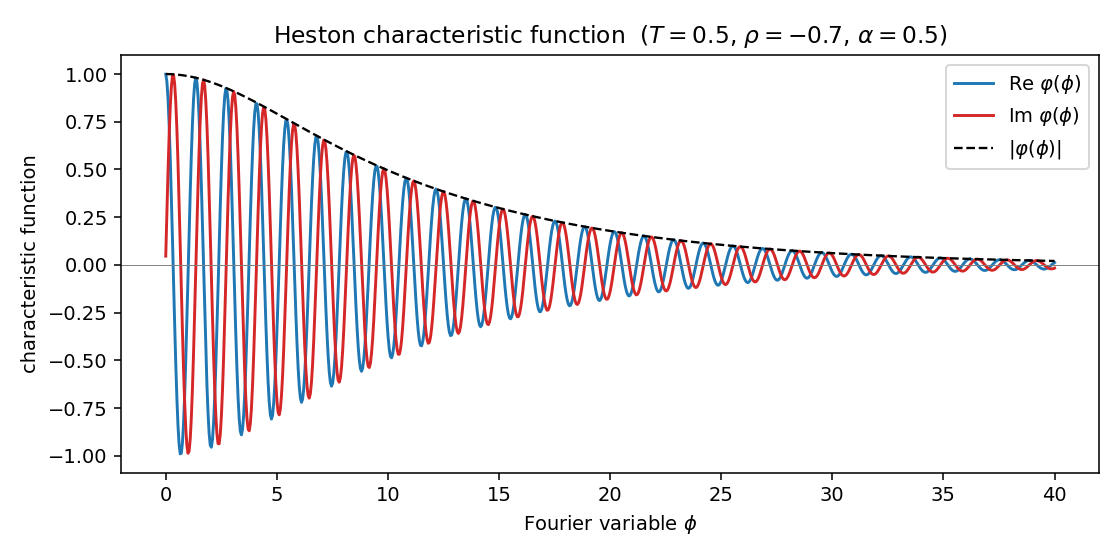
\includegraphics[keepaspectratio]{figures/ch10-heston-charfunc.png}}
\emph{Re, Im and magnitude of \(\varphi(\phi)\) for the base Heston
parameters. The rapid decay in \(|\varphi|\) is what guarantees the
Gil--Pelaez integrand
\(\mathrm{Re}[e^{-i\phi\ln K}\varphi_j(\phi)/(i\phi)]\) is absolutely
integrable and hence Fourier-invertible.}

with \[
\varphi_2(\phi) = \varphi(\phi;\,t, x, v),
\qquad
\varphi_1(\phi) = \frac{\varphi(\phi - i;\,t, x, v)}{\varphi(-i;\,t, x, v)}.
\tag{10.42}
\] (Division by \(\varphi(-i) = F_t\) normalises the density for the
share measure. With \(X_T = \ln F_T\), \(\varphi(-i) =
\mathbb{E}_t[e^{-i\cdot i X_T}] = \mathbb{E}_t[e^{X_T}] =
\mathbb{E}_t[F_T] = F_t\) because \(F\) is a \(\mathbb{Q}\)-martingale
in the futures frame, so the ratio \(F_t/F_t = 1\) drops out cleanly
inside the Gil-Pelaez integrand. In the spot frame under \(\mathbb{Q}\)
the analogous normaliser would instead be \(S_t\,e^{r\tau}\), but we
have chosen the futures frame throughout this chapter.)

The shift by \(-i\) in \(\varphi_1\) is the Esscher-transform
fingerprint of the measure change to the share measure. Under the share
measure, \(F\) is the numeraire, and densities get reweighted by
\(F_T / (F_t e^{r\tau})\). On the characteristic function, this
reweighting translates exactly to a complex argument shift of \(-i\).
This is a general trick: any ``forward-measure'' or ``share-measure''
probability can be computed from the original characteristic function by
shifting \(\phi\) appropriately, without ever redoing the derivation
under the new measure. The underlying mechanism is the same
numeraire-change machinery introduced in Chapter 5: the Radon--Nikodym
density process is \(F_T / (F_t e^{r\tau})\), so multiplying by
\(e^{i\phi X_T}\) and renormalising amounts to shifting the Fourier
argument by \(-i\).

The Esscher transform is named after Swedish actuary Fredrik Esscher,
who introduced it in 1932 in the context of insurance risk. It has deep
connections to exponential tilting in statistics and to
change-of-measure arguments in finance. The general idea: given a
characteristic function \(\varphi(\phi)\) of \(X\), the tilted
characteristic function \(\varphi(\phi + i\alpha)/\varphi(i\alpha)\)
corresponds to a new measure under which \(X\)'s density is multiplied
by \(e^{\alpha X}\) and renormalised. For \(\alpha = 1\) this is the
share-measure in finance; for other \(\alpha\) values it is the Esscher
principle for pricing under a risk-neutral measure chosen to match a
specific expectation. Whenever you see a characteristic- function shift
by \(\pm i\) or \(\pm i\alpha\), there is a change of measure hiding in
it.

Why is this useful? Because the Heston characteristic function was
derived once, for \(X = \ln F_T\), under the \(\mathbb{Q}\) measure. The
complex shift lets us re-use that one characteristic function to compute
probabilities under a family of related measures (share measure, forward
measure, etc.) at zero additional derivation cost. This is a significant
computational benefit: the Heston characteristic function evaluation
dominates the runtime of Fourier-inversion pricing, so being able to
re-use it under multiple measures saves substantial work.

\textbf{The Heston call price.} \[
\boxed{\;
C^{\text{Heston}}(t, F_t, v_t; K, T) \;=\; e^{-r\tau}\big[F_t\,P_1 \;-\; K\,P_2\big]
\;}
\tag{10.43}
\] Put is by put-call parity. One integral per probability, computed by
Gauss--Laguerre / FFT / Carr--Madan in practice.

The ``one integral per probability'' line is important for performance.
In a large calibration problem you might price several thousand options
--- every strike and maturity on a dense grid --- and each one requires
two Gil--Pelaez integrals. With 64 quadrature nodes per integral, that
is over a million characteristic function evaluations per calibration
iteration. This sounds expensive, but each evaluation is essentially a
handful of complex exponentials, and the whole calibration completes in
under a second on modern hardware. Carr--Madan FFT collapses the
computation further by pricing an entire log-strike curve in a single
FFT, dropping the cost per option to effectively zero. This is why
FFT-based Heston calibration is the industry default.

The Carr--Madan idea is worth savouring. If you write the call price as
a Fourier integral over strike, you notice that the integrand depends on
strike only through \(e^{-i\phi \ln K}\). This means that fixing the
quadrature points in \(\phi\) and then scanning strike is just a Fourier
transform of a weighted characteristic function evaluated at those
\(\phi\)-points. The Fast Fourier Transform (FFT) accomplishes exactly
this --- it transforms a sequence of function values into a sequence of
Fourier coefficients (or vice versa) in \(O(N \log N)\) time, where
\(N\) is the number of points. By sampling \(\phi\) on a regular grid
with appropriate spacing and performing an FFT, Carr and Madan produce
the entire log-strike curve of call prices in a single pass. The
implementation is elegant: choose an \(\eta\) damping, compute
\(\psi(\phi)\) at the grid of \(\phi\)-points, FFT to get the log-strike
curve, read off prices at desired strikes by interpolation. Total cost:
one \(N\)-point FFT (a few milliseconds for \(N = 4096\)) regardless of
how many strikes are needed.

Before Carr--Madan (1999), pricing a full smile for a single maturity
required one Gil--Pelaez integral per strike per probability ---
typically 20 strikes \(\times\) 2 probabilities \(\times\) 64 quadrature
nodes = 2560 characteristic-function evaluations per smile. Carr--Madan
reduced this to a single FFT with 4096 characteristic-function
evaluations, which priced the entire smile at once. The net speedup is
modest on a single smile but compounds dramatically in calibration where
you price thousands of options per iteration. Modern Heston calibration
is Carr--Madan plus a Levenberg--Marquardt optimiser, and this
combination reliably calibrates SPX to within basis-point RMS error in
under a second.

\textbf{Carr--Madan alternative.} Dampen the payoff by \(e^{\eta x}\)
and transform: \[
C = \frac{e^{-\eta\ln K - r\tau}}{\pi}\int_0^{\infty}\operatorname{Re}\!\left[e^{-i\phi\ln K}\,\psi(\phi)\right]\mathrm{d}\phi,
\qquad
\psi(\phi) = \frac{\varphi(\phi - (\eta+1)i)}{\eta^2 + \eta - \phi^2 + i(2\eta + 1)\phi}.
\tag{10.44}
\] This is a single FFT over a log-strike grid --- the workhorse for
calibration.

The damping parameter \(\eta > 0\) is a free knob that practitioners
tune (usually \(\eta \in [0.5, 2]\)) to trade off between accuracy at
different strikes. A larger \(\eta\) improves accuracy for deep
out-of-the-money calls but hurts the ATM region; a smaller \(\eta\) is
more uniform across strikes. Rule of thumb: \(\eta = 0.75\) is a
reasonable default for most equity calibrations. Pick a bad \(\eta\) and
your far-OTM prices will be inaccurate to several percent, which is
enough to throw off the wings of your calibrated smile.

The need for damping exists because the raw call-price integrand is not
absolutely integrable as a function of \(\phi\) --- it has an
\(O(1/\phi)\) decay that is borderline for convergence. Multiplying by
\(e^{\eta \ln K} = K^\eta\) (equivalently, damping the payoff by
\(e^{\eta x}\) in the strike domain) shifts the decay to exponential and
makes the integral convergent. The catch is that the damping shifts
weight toward high-\(K\) regions --- deep OTM calls --- and away from
low-\(K\) regions. Asymmetric damping is the price we pay for using a
single-sided call-price transform. An alternative approach, sometimes
called the ``generalised FFT,'' uses a symmetric combination of call and
put prices and eliminates the \(\eta\) dependence, but at the cost of
more bookkeeping. Most practitioners stick with Carr--Madan and tune
\(\eta\) for their typical strike range.

A related numerical note: the FFT log-strike grid spacing and the
\(\phi\) grid spacing are reciprocally related via the FFT Nyquist
constraint. If you want strike resolution \(\Delta \ln K = 0.01\)
(roughly 1\% moneyness resolution), you need \(\phi\) grid extending to
\(2\pi/\Delta \ln K \approx 628\). With 4096 FFT points, the \(\phi\)
spacing is roughly \(0.15\), and the integration captures the
characteristic-function contribution down to \(\phi\) roughly equal to
that spacing. For Heston, the characteristic function decays rapidly
above \(\phi \sim 10\), so these grid parameters produce negligible
truncation error. Finer grids are used for deep OTM calibration or for
improved accuracy in the extreme tails.

\begin{center}\rule{0.5\linewidth}{0.5pt}\end{center}

\section{10.7 Greeks and calibration
notes}\label{greeks-and-calibration-notes}

Five risk-neutral parameters \((\kappa, \theta, \alpha, \rho, v_0)\)
plus \(r\). Each has a clean economic role:

{\def\LTcaptype{none} % do not increment counter
\begin{longtable}[]{@{}
  >{\raggedright\arraybackslash}p{(\linewidth - 4\tabcolsep) * \real{0.3333}}
  >{\raggedright\arraybackslash}p{(\linewidth - 4\tabcolsep) * \real{0.3333}}
  >{\raggedright\arraybackslash}p{(\linewidth - 4\tabcolsep) * \real{0.3333}}@{}}
\toprule\noalign{}
\begin{minipage}[b]{\linewidth}\raggedright
Parameter
\end{minipage} & \begin{minipage}[b]{\linewidth}\raggedright
Role
\end{minipage} & \begin{minipage}[b]{\linewidth}\raggedright
Empirical sign (equity)
\end{minipage} \\
\midrule\noalign{}
\endhead
\bottomrule\noalign{}
\endlastfoot
\(v_0\) & instantaneous variance & matches ATM level \\
\(\theta\) & long-run variance & matches long-dated ATM \\
\(\kappa\) & mean-reversion rate & term-structure slope \\
\(\alpha\) & vol-of-vol & smile curvature (convexity) \\
\(\rho\) & spot/vol corr. & smile skew (negative \(\rho\)
\(\Rightarrow\) left skew) \\
\end{longtable}
}

The parameter identification story is crisp, and this is one of Heston's
greatest practical virtues. Different features of the implied vol
surface map cleanly to different parameters, so the calibration problem
is well-posed and the fitted parameters are stable across days. If the
overall level of your vol surface rises by 2 points, \(v_0\) and
\(\theta\) rise; if the skew steepens, \(\rho\) becomes more negative;
if the wings puff out, \(\alpha\) increases. Rarely does moving one
parameter require compensating moves in another to stay on-surface, and
when it does, the required compensation is modest.

Here is the quantitative version of the parameter-sensitivity story,
useful for debugging calibration. The Heston ATM implied vol at maturity
\(T\) is approximately \(\sqrt{m_T}\) where \(m_T = \mathbb{E}[v_T]\)
follows the exponential relaxation formula. Differentiating ATM vol with
respect to parameters: \(\partial \mathrm{ATM}/\partial v_0\) is nonzero
but decays with \(T\) (short-dated ATM sensitive to \(v_0\), long-dated
not); \(\partial \mathrm{ATM}/\partial \theta\) grows with \(T\)
(long-dated ATM tracks \(\theta\));
\(\partial \mathrm{ATM}/\partial \kappa\) is the blend-rate sensitivity.
The short-maturity ATM skew (slope of smile at the money) is
approximately \(\rho \alpha / (4\sqrt{v_0})\) --- a \emph{finite}
constant as \(T \to 0\) --- so \(\rho\) and \(\alpha\) both enter
multiplicatively. The ATM convexity (curvature of smile) is
approximately \(\alpha^2 T / (v_0 \kappa)\) for moderate \(T\), so this
is primarily an \(\alpha\) sensitivity. These formulas are
approximations, but they capture the dominant structure and are
extremely useful for parameter identification.

When calibration is well-posed, the Jacobian matrix of calibration
residuals with respect to parameters is well-conditioned, and
Levenberg--Marquardt converges rapidly. When it is ill-posed, the
Jacobian has near-zero eigenvalues corresponding to parameter
combinations that are under-determined. A common sign of ill-posedness
is \(\alpha\) and \(\rho\) drifting together in a correlated way ---
indicating that the calibration cannot distinguish between them on the
data. This is most likely to happen when only ATM quotes are available
(no skew information) or when the maturity range is too narrow. The
remedy is to include more smile points across strikes and more
maturities in the calibration.

Calibration targets the smile, not the term structure. This is an
important practitioner truth. Heston has a five-parameter structure and
is trying to fit what is typically a two-dimensional surface --- strikes
across maturities. In practice, the model captures the smile (variation
across strikes for a fixed maturity) much better than it captures the
full term structure of the smile (how the smile changes with maturity).
If you calibrate Heston to the full surface, you get parameters that are
a compromise --- they neither fit short-dated smiles well nor long-dated
smiles well. The standard practitioner workflow is to calibrate to a
single representative maturity (say three months), accept that shorter
and longer maturities will be imperfect, and use a richer model (or a
term-dependent extension) when the term structure matters. The
flat-term-structure failing is one of Heston's blind spots, and we come
back to it below.

The term-structure fit problem has a specific structure that is worth
understanding. At very short maturity, Heston's smile is controlled
mostly by \(v_0\) (the starting variance) and the short-time asymptotics
of the Riccati solution. The ATM vol matches \(\sqrt{v_0}\) and the
short-time ATM skew is \(\rho \alpha / (4\sqrt{v_0})\) (Durrleman 2003;
Gatheral 2006) --- a bounded constant as \(T \to 0\). Real short-dated
smiles, in contrast, exhibit a skew that \emph{grows} as maturity
shortens (empirically like \(T^{-H}\) with \(H \in (0, 1/2)\)), so
Heston \emph{understates} the short-dated skew relative to market. At
long maturity, the skew decays faster than \(1/\sqrt{T}\) because the
variance has time to mean-revert and average out the correlation effect.
The full term-structure shape implied by Heston is ``steep skew at short
dates, flat skew at long dates'' --- which matches the qualitative
pattern of real smiles but rarely the quantitative shape. Markets
typically have ``steep skew at short dates, less-steep but still-steep
skew at intermediate dates, and flatter skew at very long dates'' --- a
more gradual decay that Heston cannot match with constant parameters.

This is where term-dependent Heston comes in. Let \(\kappa\),
\(\theta\), \(\alpha\), \(\rho\) all be piecewise-constant functions of
time, with breakpoints at the maturities of traded options. The
characteristic function can still be computed (by integrating the
Riccati ODE piecewise in time), and the model can now match the full
term structure exactly. The downside is parameter proliferation --- now
you have \(5 \times N\) parameters for \(N\) maturity buckets --- and
calibration becomes more delicate. But for desks that need to match
long-dated exotic books to the traded surface exactly, term-dependent
Heston is the workhorse. Some implementations go further and treat
\(v_0\) as a ``state'' while calibrating
\(\kappa(t), \theta(t), \alpha(t), \rho(t)\) as ``parameter functions''
--- this maintains Markov consistency while adding flexibility.

\pandocbounded{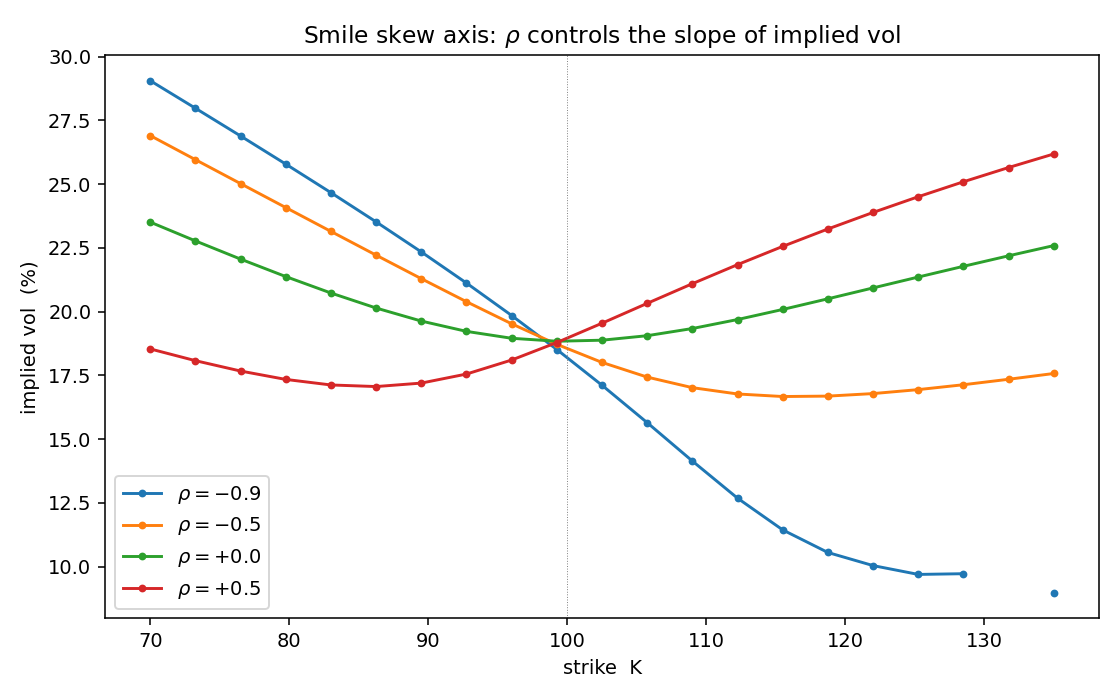
\includegraphics[keepaspectratio]{figures/ch10-heston-skew-vs-rho.png}}
\pandocbounded{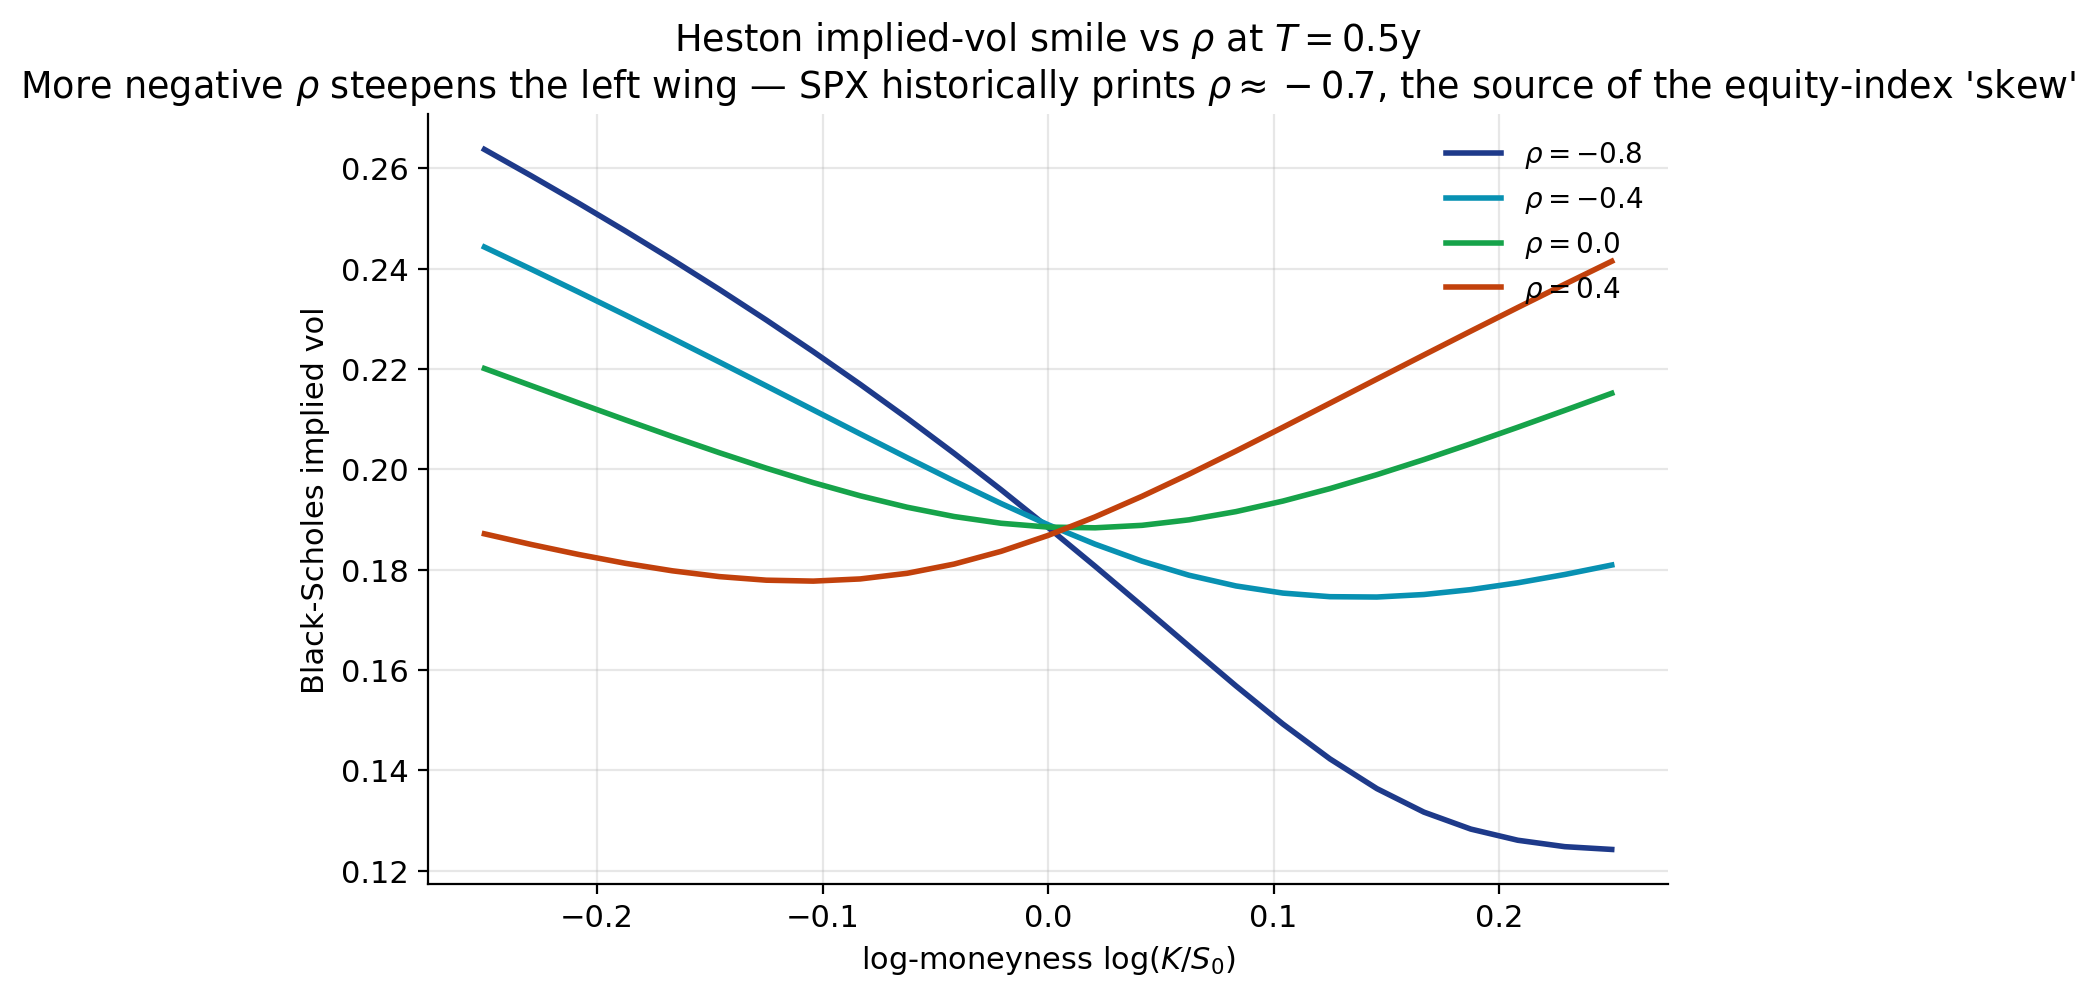
\includegraphics[keepaspectratio]{figures/ch10-smile-vs-rho.png}}
\emph{Heston smile for \(\rho \in \{-0.9, -0.5, 0, +0.5\}\), holding
\((\kappa, \theta, \alpha, v_0)\) fixed. Negative \(\rho\) tilts the
smile down-right (equity left-skew); positive \(\rho\) tilts it up-right
(FX or commodity inverted-skew). The ATM point barely moves --- \(\rho\)
is a pure slope control.}

Notice how remarkably clean the rotation is: as \(\rho\) sweeps from
negative through zero to positive, the smile pivots around its ATM
point. This is the cleanest visual demonstration of what it means to say
``\(\rho\) controls the skew.'' Notice also that the ATM level is
essentially invariant --- changing \(\rho\) by \(\pm 0.3\) moves the
25-delta implied vols meaningfully but leaves the 50-delta ATM vol
essentially unchanged. This clean decomposition is what makes Heston
calibration well-posed.

In the language of risk reversals, the 25-delta risk reversal ---
defined as the difference between 25-delta call vol and 25-delta put vol
--- is essentially proportional to \(\rho\) at fixed maturity. A risk
reversal of zero corresponds to \(\rho = 0\); a positive risk reversal
(calls dearer than puts) corresponds to \(\rho > 0\); a negative risk
reversal corresponds to \(\rho < 0\). The approximate proportionality
coefficient is \(\alpha / \sqrt{v_0} \sqrt{T}\), so at fixed \(\alpha\)
and \(v_0\), the risk reversal decays as \(1/\sqrt{T}\). Real markets
show a similar pattern, which is part of why Heston matches the
qualitative term structure of risk reversals reasonably well. The
cleanness of the \(\rho\)-to-risk-reversal mapping is what lets traders
calibrate \(\rho\) almost by inspection of the risk reversal quote for a
representative maturity.

The visual symmetry of the \(\rho\)-sweep also demystifies what is
sometimes called ``sticky-delta'' vs ``sticky-strike'' behaviour. In a
Heston world with \(\rho < 0\), the smile tilts downward to the right;
when spot moves, the delta coordinates of the options shift, and the
vols at fixed delta stay roughly the same (sticky-delta behaviour).
Heston therefore naturally generates sticky-delta dynamics, which is the
empirical behaviour observed in FX and less-systematically in equities.
Models with different dynamics (pure local vol) tend to generate
sticky-strike behaviour (vols at fixed strike stay the same), which is
less empirically supported. This is an underappreciated advantage of
stochastic vol over local vol for forward-smile modelling.

\pandocbounded{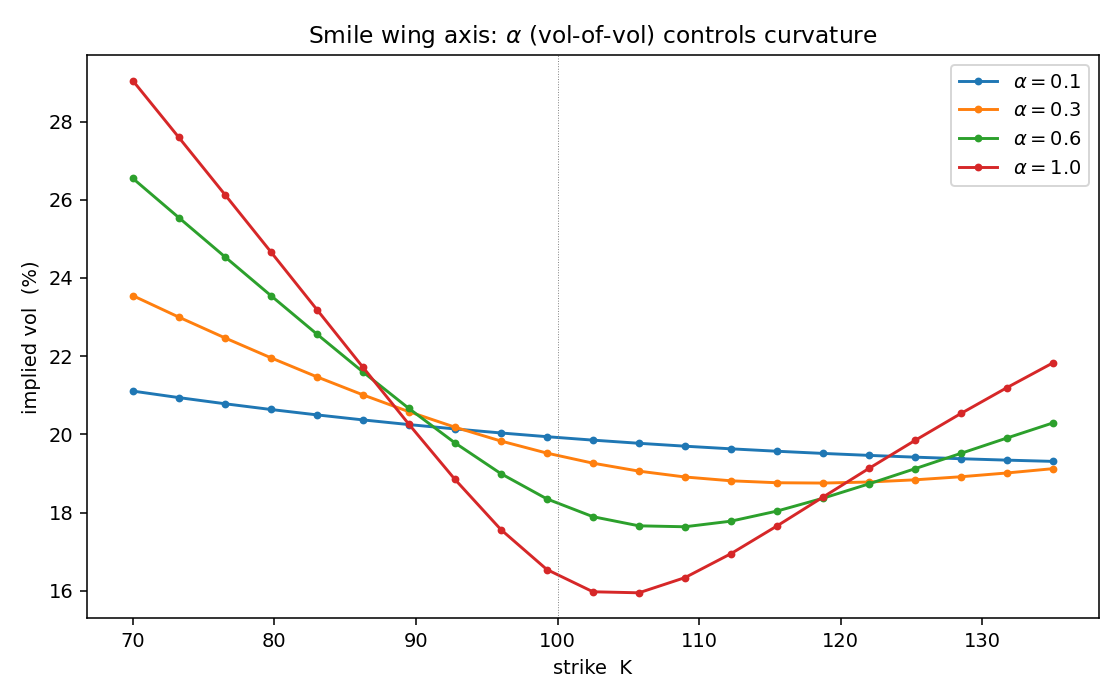
\includegraphics[keepaspectratio]{figures/ch10-heston-wings-vs-volvol.png}}
\pandocbounded{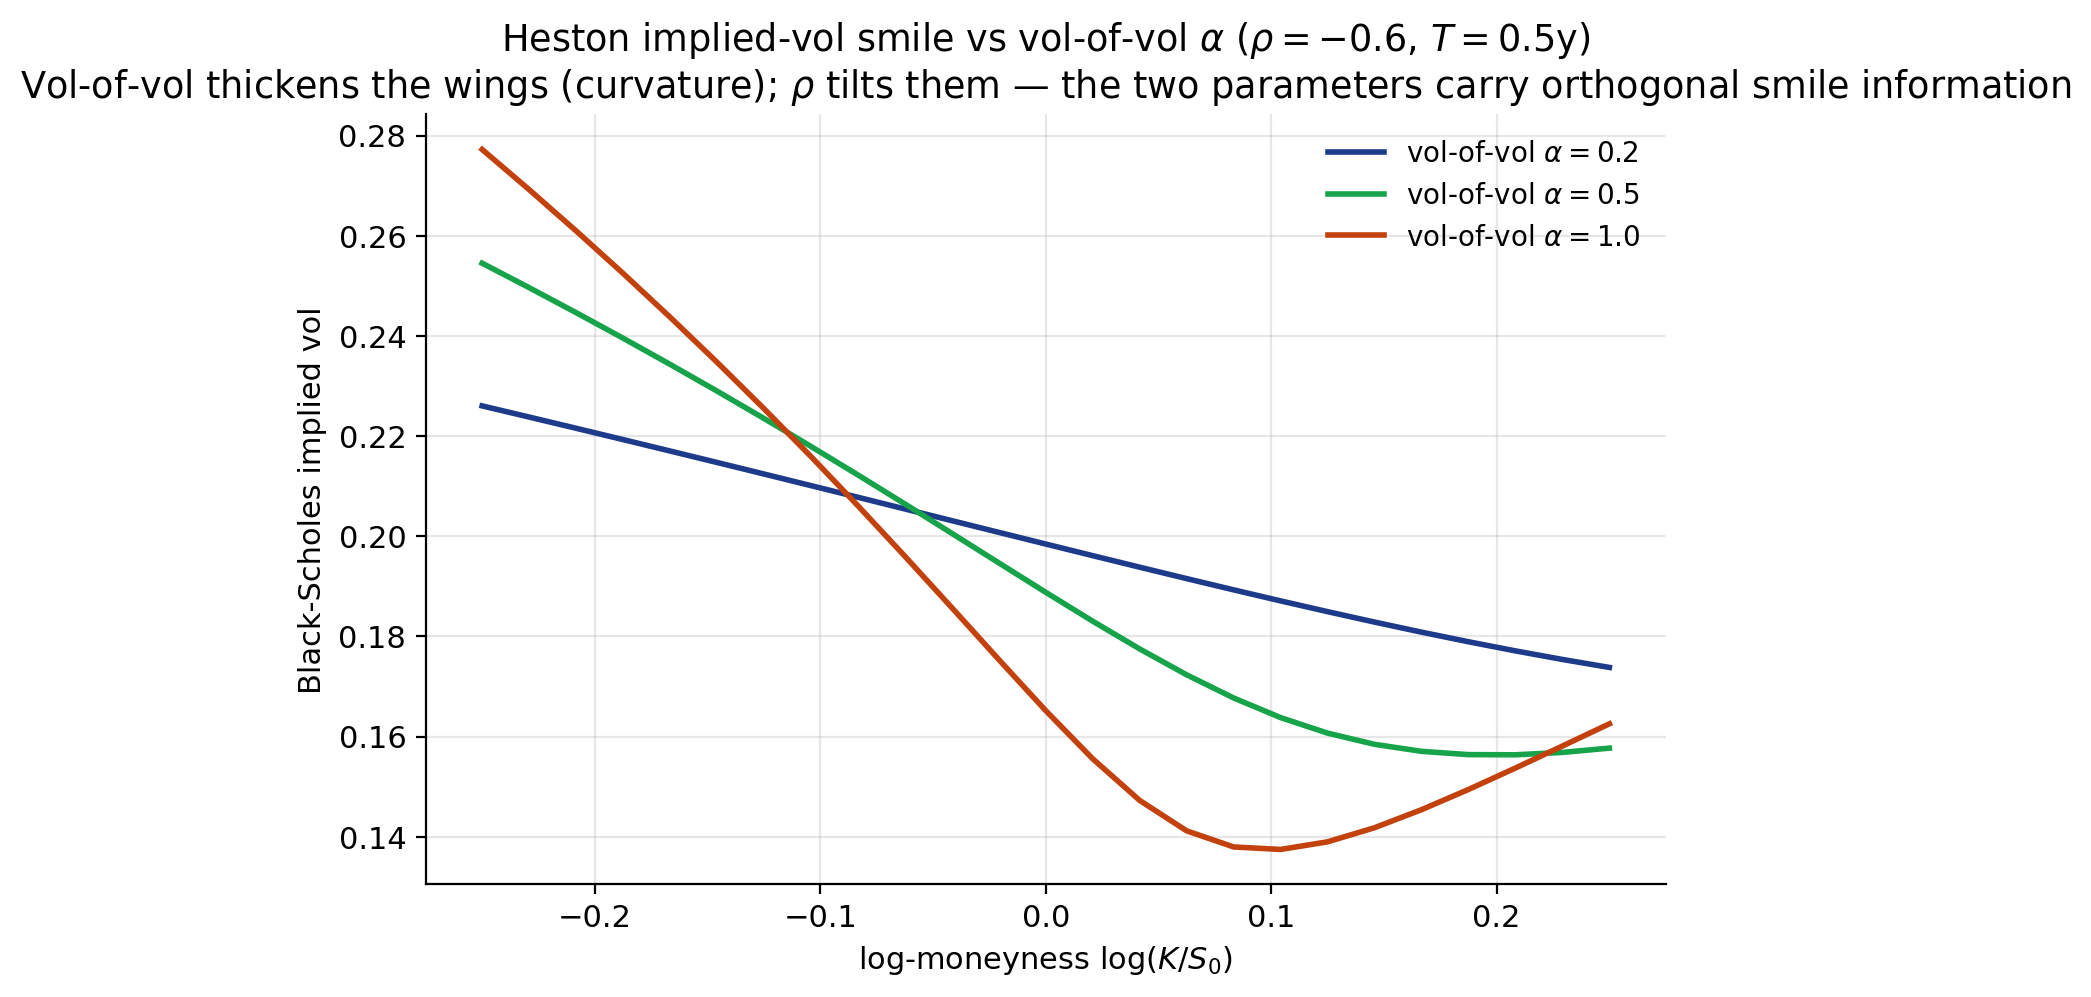
\includegraphics[keepaspectratio]{figures/ch10-smile-vs-volvol.png}}
\emph{Smile curvature grows with \(\alpha\). Small \(\alpha\) (weak
vol-of-vol) flattens the smile toward the BS line; large \(\alpha\)
lifts both wings --- deep puts and deep calls both gain, symmetrically
around the mild \(\rho = -0.3\) tilt.}

The complementary picture for \(\alpha\): increase vol-of-vol and both
wings lift together, preserving the skew that \(\rho\) encoded. Think of
\(\alpha\) as the ``wingspan'' parameter. A flat Black--Scholes smile
corresponds to \(\alpha = 0\) (deterministic variance). As \(\alpha\)
grows, the mixture of lognormals becomes more heterogeneous --- some
paths are much more volatile than others --- and the resulting
unconditional distribution has fatter tails, hence higher implied vols
at the wings. In the limit of very large \(\alpha\) (and Feller severely
violated), the smile becomes so steep at the wings that the density
takes on heavy-tail features approaching Student-\(t\) behaviour.

The 25-delta butterfly --- the average of 25-delta call and put vols
minus ATM vol --- is the market quote that directly reflects \(\alpha\).
A butterfly of zero means a flat smile, consistent with \(\alpha = 0\).
A positive butterfly means both wings are richer than ATM, which maps to
\(\alpha > 0\). In the approximate asymptotic formula, the butterfly
scales roughly as \(\alpha^2 \kappa^{-1}\) with a mild \(T\)-dependence.
The cleanness of this mapping means that, like
\(\rho\)-to-risk-reversal, the \(\alpha\)-to-butterfly mapping can be
read off approximately by eyeballing the butterfly at a representative
maturity.

When calibrators describe a surface with ``rich wings,'' they mean a
high butterfly. This maps to high calibrated \(\alpha\), which in turn
triggers Feller-violation diagnostics. Hence the indirect but real
connection between rich-wing smiles, high vol-of-vol, and
Feller-boundary behaviour. Surfaces with near-flat wings (low butterfly,
typical of calm FX markets) calibrate to \(\alpha \approx
0.3\) or less and are comfortably Feller-safe. Surfaces with very rich
wings (high butterfly, typical of stressed equity markets) calibrate to
\(\alpha > 0.7\) and may violate Feller aggressively. The relationship
between market feature (butterfly), calibrated parameter (\(\alpha\)),
and diagnostic (Feller violation) is clean and traceable.

\subsection{10.7.1 Greeks}\label{greeks}

Because \(C = e^{-r\tau}(F\,P_1 - K\,P_2)\) and \(P_1, P_2\) depend on
\(v\) only through \(B(\tau)\,v\) in \(\varphi\): \[
\Delta_F = \frac{\partial C}{\partial F} = e^{-r\tau} P_1,
\tag{10.45}
\] \[
\mathcal{V}_v = \frac{\partial C}{\partial v_0} = e^{-r\tau}\!\left(F\,\frac{\partial P_1}{\partial v} - K\,\frac{\partial P_2}{\partial v}\right),\qquad
\frac{\partial P_j}{\partial v} \text{ via differentiating (10.41) under the integral.}
\tag{10.46}
\] Vega in the Heston sense is with respect to \(v_0\), not BS
\(\sigma\).

This is a subtle point worth emphasising. When a practitioner says
``vega,'' they typically mean Black--Scholes vega --- the sensitivity of
the option price to the Black--Scholes implied volatility. In Heston,
the natural vega is with respect to \(v_0\), the current instantaneous
variance. These two vegas are related but not identical; they differ by
a Jacobian that depends on the full set of Heston parameters. If your
hedging is driven by Heston, you should hedge \(\mathcal{V}_v\); if your
hedging is driven by BS conventions (e.g.~if you quote in BS vega
terms), you can convert back via the chain rule. A deeper practitioner
insight: in Heston, vega is only one of many vol-sensitivity parameters.
You also have sensitivities to \(\kappa\), \(\theta\), \(\alpha\), and
\(\rho\). Each of these is a degree of freedom in the model that can
move, and a complete hedging programme would neutralise each of them ---
the so-called model-risk hedge, as distinct from the delta/vega hedge.

In practice, delta-vega hedging in Heston is close enough to
BS-delta-vega hedging that most desks treat them interchangeably for
vanilla books. The real divergence shows up for path-dependent products.
Consider a barrier option. In BS, the barrier risk is hedged by matching
the terminal payoff; in Heston, the barrier risk is coupled to vol
dynamics because vol spikes can push spot through the barrier. A
Heston-consistent barrier hedge uses not just delta and vega but also
vanna (the cross sensitivity) and volga (the second vega). These
higher-order Greeks are straightforward to compute in Heston via
numerical differentiation of the characteristic-function price, and
their management is a major focus of exotic desks. For a vanilla book,
higher-order Greeks matter less but still exist; ignoring them is a
source of hedge slippage over time.

A related concept: the concept of ``Heston vega'' as distinct from ``BS
vega'' becomes important when you discuss the cost of a vega hedge. In
BS, the vega hedge is obtained by buying or selling a liquid option to
offset the position's BS-vega. In Heston, a vega hedge must offset the
sensitivity to \(v_0\), which depends on the Heston parameters. The
quantitative difference is typically small but can be meaningful for
large positions or for positions with significant vol convexity. Many
production systems compute both BS-vega (for P\&L attribution) and
Heston-vega (for hedging) simultaneously and report both. The gap
between them is the ``model-convexity'' adjustment.

One more consideration: in a Heston world, the natural vol risk to hedge
is often the variance-swap risk, not the \(v_0\) risk. The variance swap
has a linear payoff in realised variance and provides a clean way to
hedge the integrated-variance exposure that options carry. Many exotic
desks run a hybrid hedging programme: delta on spot, \(v_0\)-vega on
options (for short-term risk), variance-swap hedges (for long-term
integrated-variance risk), and periodic rebalancing as the vol regime
changes. This layered hedging approach is more robust than pure BS-vega
hedging and is a direct consequence of thinking in Heston terms rather
than BS terms.

\subsection{10.7.2 Calibration workflow
(practitioner)}\label{calibration-workflow-practitioner}

\begin{enumerate}
\def\labelenumi{\arabic{enumi}.}
\tightlist
\item
  Snap an implied-vol surface (liquid listed options).
\item
  Choose a loss
  \(L = \sum_i w_i (\sigma^{\text{mkt}}_i - \sigma^{\text{Heston}}_i)^2\)
  (IV RMS) or price-RMS.
\item
  Minimise by Levenberg--Marquardt / differential evolution. Start at
  \(\rho < 0\), \(v_0 \approx (\sigma^{\text{ATM}})^2\),
  \(\theta \approx v_0\), \(\kappa \in [1, 5]\),
  \(\alpha \in [0.3, 1.0]\).
\item
  Check Feller; if violated, use full-truncation MC for path-dependent
  payoffs.
\item
  Re-calibrate daily; watch for \(\rho\) jumps (data artefact) or
  \(\alpha\) blowups (ill-posed surface).
\end{enumerate}

\textbf{Generic practitioner notes (to move to Chapter 11):} IV-RMS vs
price-RMS weighting; basin-of-attraction starting values; multi-target
calibrations per product class; time-smoothness and Bayesian
regularisation; two-stage SVI-prefit-then-Heston pipelines; pre-event
masking for known jumps. These are general non-linear-least-squares
hygiene rules; nothing Heston-specific.

\textbf{Heston-specific calibration notes.} \(\rho\) and \(\kappa\)
should be stable day-to-day in stable regimes; sudden jumps signal data
or regime issues. The five Heston parameters trade off in well-known
ways: \((\kappa, \theta)\) determine the term structure;
\((\alpha, \rho)\) determine the smile shape per expiry; \(v_0\) anchors
the short end. Surface inability to simultaneously fit short and long
dates is a Heston blind spot (§10.10), not a calibration failure.

Residual diagnostics: smile-shaped residual at short end + flat at long
end \(\to\) calibration is targeting long-dated;
wing-positive/middle-negative residuals across maturities \(\to\)
\(\alpha\) too small; put-negative/call-positive \(\to\) \(\rho\) wrong
sign.

\subsection{Case study (b): March 2020 COVID --- vol surface explodes
from 12 to
80}\label{case-study-b-march-2020-covid-vol-surface-explodes-from-12-to-80}

\emph{VIX 14 \(\to\) 82 in 18 trading days; the entire vol surface
levitated.} \emph{Heston re-calibration shows \(v_0\) jumping
5--10\(\times\), \(\xi\) doubling.} \emph{Production desks moved from
1\(\times\) to 4--6\(\times\) daily re-calibration intraday.}

\textbf{Context.} Between Wednesday 19 February and Monday 16 March
2020, the VIX rose from 13.68 to 82.69 --- its highest closing level on
record at that time, surpassing the 80.86 close from the November 2008
GFC peak. The S\&P 500 fell from 3393.52 (Feb 19) to 2480.64 (Mar 12, an
11-day sequence of −3\% to −10\% daily prints), and to 2304.92 (Mar 23
intraday trough). On the option side, the entire vol surface levitated:
ATM implied vols on 30-day SPX rose from \textasciitilde12\% to
\textasciitilde70\%; the persistent post-1987 skew (case study a)
flattened materially as panic-driven OTM put buying narrowed the
relative gap between ATM and the wings; longer tenors (1y, 2y) rose less
than 30-day but still doubled or tripled. For options dealers (the
Greek-letter sell-side: Goldman, Citi, JPM, MS, Susquehanna), every
Heston-calibrated book was repricing daily by tens to hundreds of
millions on the vega component alone.

The mechanical impact on a desk MTM was direct. A typical SPX vol-desk
book runs a vega notional in the \$20--100M per vol-point range,
computed across the surface. ATM vega P\&L = \(\Delta\sigma \times\)
vega; a +5 vol-point day on a \$50M-vega book is a \$250M MTM mark. The
first week of the COVID move (20 Feb -- 28 Feb) saw some desks book
\$200M+ in vega P\&L per day from realised gamma alone (long-vol books)
or from forced delta-rebalancing of structurally short-vol positions
(short-vol books). The intraday MTM volatility was severe enough that
the post-2020 review period at most major dealers tightened intraday
risk-limit refresh cadence.

\textbf{Through the chapter's math.} Heston re-calibration through the
Feb-March 2020 period shows three near-simultaneous parameter shifts.
Pre-crisis (Feb 2020) calibration on a 30-day liquid SPX surface gave
roughly \(v_0 \approx 0.014\) (\textasciitilde12\% vol),
\(\theta \approx 0.030\) (\textasciitilde17\% long- run vol),
\(\kappa \approx 4\), \(\xi \approx 0.55\), \(\rho \approx -0.75\).
Mid-March 2020 calibration on the same surface gave \(v_0 \approx 0.16\)
(\textasciitilde40\% vol; up by a factor of \textasciitilde10),
\(\theta \approx 0.060\) (\textasciitilde25\%; up roughly 2\(\times\)),
\(\kappa\) roughly stable at \(\sim 3\), \(\xi \approx 1.2\) (roughly
2\(\times\)), \(\rho \approx -0.40\) (the skew flattened --- case study
a's ``leverage parameter'' measurably weakened in the panic, as ATM and
OTM both bid). The Greeks the desk cared about were
\(\partial V/\partial v_0\) (short-end vega),
\(\partial V/\partial \xi\) (volga, vol-of-vol exposure), and
\(\partial V/\partial \rho\) (the skew Greek). For a typical \(50M-vega
ATM book, the volga exposure (\)\partial\^{}2
V/\partial v\_0,\partial \xi\$ in Heston language) was the
second-largest Greek by P\&L impact and was materially under-hedged on
most desks pre-COVID.

\textbf{Lesson.} The five Heston parameters are not eternal constants
--- they are slow-moving state variables, and in genuine regime change
they become \emph{fast}-moving. Two operational consequences. First, the
standard once-daily Heston re-calibration cadence (snap surface at the 4
PM close, fit, run risk on the new parameters until the next close) is
inadequate in stress regimes; a vol surface that levitates 30 points
between the open and the close has produced six-figure MTM moves on
every single contract before the calibration catches up. Post-COVID
production cadence at the major dealers moved to 4--6 intraday
re-calibrations during stress periods (typically 9:45, 11:00, 13:00,
14:30, and 15:45 ET on US trading days), with bespoke event-driven runs
around scheduled news. Second, the desk's risk limits should be
expressed not just in vega but in the \emph{full} Heston-Greek vector
including volga and the skew Greek; a book that is vega-flat but volga-
long can take a six-sigma loss on a vol-of-vol regime change with no
warning from the daily VaR system. The lesson for the Chapter-10 reader
is operational: the elegance of Heston's five-parameter parsimony is a
feature in calm markets and a liability in regime change, and the
production response is to instrument the parameter trajectories
themselves as risk variables.

\begin{center}\rule{0.5\linewidth}{0.5pt}\end{center}

\section{10.8 Variance swaps}\label{variance-swaps}

A variance swap pays realised variance minus a strike at \(T\). The
realised variance is \[
\text{"realised variance"} \;\stackrel{\Delta}{=}\; \sum_{n=1}^{N}\!\left(\frac{F_{t_n}}{F_{t_{n-1}}} - 1\right)^{\!2} = R,
\tag{10.47}
\] pay-off at \(T\): \[
\text{Pays}\;(R - K)\;@\;T.
\tag{10.48}
\]

A variance swap pays on total realised variability --- ``pure vol
exposure,'' delta-neutral, vega-one. Demeterfi--Derman--Kamal--Zou
(1999) showed the model-free log-contract replication via a static
portfolio of options plus dynamic delta hedge, which is also the basis
of the VIX formula. The 2008 crisis exposed jump-vulnerability of the
replication, motivating capped variance swaps and the shift toward
VIX-based vol products.

Use
\(\frac{F_{t_n}}{F_{t_{n-1}}} - 1 \approx \frac{\mathrm{d}F_t}{F_t}\) on
a fine grid, so \[
R \;\simeq\; \sum_{n=1}^{N}\!\left(\frac{\mathrm{d}F_{t_n}}{F_{t_n}}\right)^{\!2}.
\tag{10.49}
\] Now using (10.14) \(\frac{\mathrm{d}F_t}{F_t} = \gamma\sqrt{v_t}\,
\mathrm{d}W_t\) (with \(\gamma = 1\)), \[
R \;\simeq\; \sum_{n=1}^{N}\!\big(\gamma\sqrt{v_{t_{n-1}}}\big)^{2}\big(W_{t_n} - W_{t_{n-1}}\big)^{2}.
\tag{10.50}
\] Taking expectation, as \(N \to \infty\), the Itô isometry (Chapter 3)
turns the sum of squared Brownian increments into a time integral of the
squared diffusion coefficient: \[
\mathbb{E}[R] \;\longrightarrow\; \mathbb{E}\!\left[\int_0^{T}\gamma^2 v_s\,\mathrm{d}s\right]
= \gamma^2\int_0^{T}\mathbb{E}[v_s]\,\mathrm{d}s.
\tag{10.51}
\]

The infinite-sampling limit gives expected realised variance =
time-integral of expected instantaneous variance --- a model-free
identity that Heston makes closed-form.

\subsection{10.8.1 Expected variance under
Heston}\label{expected-variance-under-heston}

Compute \(\mathbb{E}[v_s]\) under the Heston SDE. From (10.15), \[
v_t - v_0 = \int_0^{t}\kappa(\theta - v_s)\,\mathrm{d}s + \alpha\int_0^{t}\sqrt{v_s}\,\mathrm{d}W_s^{v}.
\tag{10.52}
\] Taking expectations (the Itô integral is a martingale, expectation
zero --- the martingale property of Itô integrals proved in Chapter 3
§3.7), \[
\mathbb{E}[v_t] - v_0 = \int_0^{t}\kappa(\theta - \mathbb{E}[v_s])\,\mathrm{d}s + 0.
\tag{10.53}
\] Let \(m_t \stackrel{\Delta}{=} \mathbb{E}[v_t]\). Then \[
m_t - m_0 = \int_0^{t}\kappa(\theta - m_s)\,\mathrm{d}s,
\tag{10.54}
\] \[
\begin{cases}
\dot m_t = \kappa(\theta - m_t),\\
m_0 = v_0,
\end{cases}
\qquad\Longrightarrow\qquad
\boxed{\; m_t = v_0\,e^{-\kappa t} + \theta\,(1 - e^{-\kappa t})\;}
\tag{10.55}
\] An exponential relaxation from \(v_0\) to \(\theta\) at rate
\(\kappa\).

Expected variance is a convex combination of \(v_0\) and \(\theta\) with
weights decaying exponentially at rate \(\kappa\); \(\kappa\) is the
time-constant for variance-shock decay. The slope of the VIX term
structure carries a clean Heston interpretation: \(v_0 < \theta\) gives
a rising (contango) VIX curve, \(v_0 > \theta\) gives backwardation.

\subsection{10.8.2 Fair variance strike}\label{fair-variance-strike}

The fair strike \(K\) is the one making \(\mathbb{E}[R - K] = 0\): \[
\boxed{\;
K \;=\; \mathbb{E}[R] \;=\; \gamma^2\!\int_0^{T} m_s\,\mathrm{d}s
\;=\; \gamma^2\!\left[\theta\,T + \frac{v_0 - \theta}{\kappa}\,\big(1 - e^{-\kappa T}\big)\right]
\;}
\tag{10.56}
\] Remarkably, the fair variance strike depends only on
\((\kappa, \theta, v_0)\) --- not on \(\alpha\) and not on \(\rho\). The
vol-of-vol and correlation enter the distribution's higher moments but
not the mean.

Variance swaps and options give complementary information: variance-swap
term structure pins down \((\kappa, \theta, v_0)\) (mean dynamics,
depending only on drift parameters); options then pin down
\((\alpha, \rho)\) (shape, depending on diffusion). A two-stage
calibration is more stable than a joint five-parameter fit.

\textbf{VIX connection.} VIX is the square-root of a 30-day
variance-swap strike on SPX:
VIX\(^2 \cdot (30/365) = \int_0^{30/365} m_s\,\mathrm{d}s\). VIX futures
price forward expected integrated variance at longer horizons via
(10.56); VIX options become options on \(m_T\) --- still tractable via
the characteristic function. In Heston, VIX dynamics are
\emph{endogenous} (determined by \(v_t\) through the exponential-decay
kernel), so a single calibrated Heston can simultaneously price SPX
vanillas, variance swaps, VIX futures, and VIX options as one consistent
book.

\subsection{10.8.3 Variance swap as
tradable}\label{variance-swap-as-tradable}

Assume the swap itself is quoted with price dynamics \[
\frac{\mathrm{d}R_t}{R_t} = \sigma(v_t, t)\,\mathrm{d}W_t,
\qquad
R_0 = \hat{V}_0(T) \quad \text{— fair variance swap strike of $T$-maturity.}
\tag{10.57}
\] Payoff \((R_T - K)_{+}\) at \(T\) on this tradable now becomes a
standard option that can be solved analytically against the Heston
\(\hat V_0(T)\) curve.

This layered construction --- model vanilla options with Heston, then
use the fair variance-swap curve as a tradable to price options on
variance --- is how modern volatility desks handle the full suite of vol
products. Variance swaps become inputs to the calibration; options on
variance (like VIX options) become outputs of the calibrated model; and
the whole system is internally consistent at the level of Heston
dynamics.

One more connection to flesh out: the relationship between Heston and
VIX drives a lot of the cross-market trading activity in the vol
complex. If SPX smile calibration suggests one set of Heston parameters,
and VIX futures suggest another, the inconsistency creates a trade: sell
the over-priced side, buy the under-priced side, and wait for
convergence. This ``VIX-SPX basis'' trade is a staple of vol arbitrage
strategies, and it depends structurally on the Heston linkage between
variance dynamics and VIX. Traders who understand the Heston framework
can spot these inconsistencies cleanly; traders who do not rely on
cruder heuristics. The Heston framework therefore serves not just for
pricing but for relative-value analysis across the entire vol complex.

\begin{center}\rule{0.5\linewidth}{0.5pt}\end{center}

\section{10.9 Worked example --- Heston price
vs.~Black--Scholes}\label{worked-example-heston-price-vs.-blackscholes}

\textbf{Setup.} \(F_0 = 100\), \(r = 0\), \(T = 0.5\), \(v_0 = 0.04\),
\(\theta = 0.04\), \(\kappa = 2.0\), \(\alpha = 0.5\), \(\rho = -0.7\).
Feller: \(2\kappa\theta = 0.16 \ge 0.25 = \alpha^2\) --- violated (by a
hair); use full-truncation sim, but closed form still fine.

Grounding these parameter choices: \(v_0 = \theta = 0.04\) means the
instantaneous vol starts at and reverts to \(\sqrt{0.04} = 20\%\), a
realistic equity-ATM-vol level. The mean-reversion rate \(\kappa = 2\)
gives a six-month half-life for vol shocks, again realistic for equity
indices. The vol-of-vol \(\alpha = 0.5\) is in the upper range of
typical calibrated values and mildly violates Feller. The correlation
\(\rho = -0.7\) captures a strong leverage effect. These numbers produce
a visible but not extreme equity smile at six-month maturity.

The Feller check is a useful sanity diagnostic.
\(2\kappa\theta = 2 \times 2 \times 0.04 = 0.16\), and
\(\alpha^2 = 0.5^2 = 0.25\). The ratio is \(0.16 / 0.25 = 0.64\), so the
condition fails by a factor of \(1/0.64 \approx 1.56\) --- a mild
violation. In the stationary distribution, the variance process has a
gamma density with shape parameter \(2\kappa\theta/\alpha^2 = 0.64\),
which means the density is infinite at zero. This is a signature of
meaningful but not catastrophic Feller violation. Full-truncation MC
will work; exact MC via non-central chi-squared will be slightly more
accurate.

Note also that the choice \(v_0 = \theta\) is deliberately clean for
pedagogy. In real calibrations, \(v_0\) rarely equals \(\theta\)
exactly; usually there is a meaningful gap that reflects whether the
market is currently above or below its long-run baseline. If
\(v_0 = 0.06\) and \(\theta = 0.04\) (currently stressed), the
variance-swap curve slopes downward (backwardation); if \(v_0 = 0.02\)
and \(\theta = 0.04\) (currently calm), the curve slopes upward
(contango). The VIX term structure carries this information directly and
is a useful input to calibration.

\textbf{Step 1} --- Riccati coefficients at \(\phi = 1\) (illustration,
for \(\omega = i\)): \[
d(i) = \sqrt{(\rho\alpha i - \kappa)^2 - \alpha^2\,i(i-1)}
= \sqrt{(-0.35 i - 2)^2 - 0.25\,i(i-1)}.
\] Compute \((-0.35i - 2)^2 = 4 + 1.4 i + 0.1225 i^2 = 4 - 0.1225 +
1.4 i = 3.8775 + 1.4 i\). And \(0.25\,i(i-1) = 0.25(i^2 - i) = -0.25
- 0.25 i\). So \[
d(i)^2 = 3.8775 + 1.4 i - (-0.25 - 0.25 i) = 4.1275 + 1.65 i.
\] Take the principal square root: \(|d(i)^2| = \sqrt{4.1275^2 +
1.65^2} \approx 4.4451\), \(\arg(d(i)^2) = \arctan(1.65/4.1275)
\approx 0.3804\) rad; hence \(|d(i)| = \sqrt{4.4451} \approx 2.1083\),
\(\arg d(i) \approx 0.1902\) rad, giving
\(d(i) \approx 2.070 + 0.399 i\).

\textbf{Step 2} --- \(B, A\) at \(\tau = 0.5\) follow (10.34)--(10.35).

\textbf{Step 3} --- \(P_1, P_2\). Numerically integrate (10.41) via
Gauss--Laguerre (64 nodes) for each strike.

\textbf{Step 4} --- compare. For ATM \(K=100\): Heston IV
\(\approx 0.200\), matches \(v_0\). For \(K = 90\): Heston IV
\(\approx 0.224\) vs BS-flat \(0.200\) --- the skew. For \(K = 110\):
Heston IV \(\approx 0.186\) --- thinner right tail due to \(\rho < 0\).

Look at those three numbers in concert. The ATM implied vol matches
\(\sqrt{v_0}\), which is what we would expect: at the money, the option
is so close to delta-neutral that the tail behaviour of the density does
not affect its price much, and the Black--Scholes-comparable vol simply
reads off the level of the Heston density's standard deviation. Ten
percent out of the money on the put side (K = 90), implied vol has
lifted by about 2.4 points --- that is the combined effect of fatter
tails (\(\alpha\) contribution) and the leverage skew (\(\rho\)
contribution). Ten percent out of the money on the call side (K = 110),
implied vol has fallen by about 1.4 points --- the fatter-tail effect is
more than offset by the skew pulling right-side prices down. The
asymmetry between \(+1.4\) (down on calls) and \(+2.4\) (up on puts) is
the signature of \(\rho = -0.7\): the skew dominates the smile on the
downside.

To quantify this more carefully, consider the 25-delta risk reversal. At
six months, with these parameters, the 25-delta put would be around K =
88 and the 25-delta call around K = 113. The implied vols at these
strikes from Heston are approximately 23.0\% and 18.8\% respectively, so
the risk reversal is 23.0 - 18.8 = 4.2 points. The 25-delta butterfly is
{[}(23.0 + 18.8)/2 - 20.0{]} = 0.9 points. These numbers are close to
what you would actually see on a six-month SPX surface on a typical
trading day, so the choice of Heston parameters
\((v_0, \theta, \kappa, \alpha, \rho) = (0.04, 0.04, 2, 0.5, -0.7)\)
produces a realistic surface. This is not a coincidence --- these
parameters are broadly consistent with typical SPX calibration results.

A useful exercise is to perturb each parameter individually and observe
the effect. Move \(\rho\) from \(-0.7\) to \(-0.4\): the put IV at K=90
falls from 22.4\% toward 21.3\% (less skew), and the call IV at K=110
rises from 18.6\% toward 19.1\%, narrowing the risk reversal from 3.8 to
2.2 points. Move \(\alpha\) from 0.5 to 0.7: both wings lift, the ATM
vol stays essentially put, and the butterfly rises from 0.9 to 1.6
points. Move \(\kappa\) from 2 to 4: the term structure of smile (how
quickly it flattens with maturity) speeds up. Move \(\theta\) from 0.04
to 0.06: the long-dated ATM rises, and the short-dated smile shifts up
modestly because \(v_t\) is drifting toward a higher target. These
sensitivities are the quantitative content of ``what each Heston
parameter does,'' and working through them by hand is the best way to
internalise the model.

\textbf{Variance-swap fair strike for this parameter set:} \[
K_{\text{VS}} = \theta\,T + \frac{v_0 - \theta}{\kappa}(1 - e^{-\kappa T})
= 0.04\cdot 0.5 + 0 = 0.020 \quad (= 0.5 \times \theta, \text{ since } v_0 = \theta).
\] Annualised vol: \(\sqrt{K_{\text{VS}}/T} = \sqrt{0.04} = 0.200\) ---
as expected when \(v_0 = \theta\).

When \(v_0 = \theta\), the variance process starts at its long-run
level; there is no transient decay, and the expected integrated variance
over \([0, T]\) is simply \(\theta T\). Annualising by dividing by \(T\)
recovers \(\theta\) itself, and taking the square root gives the vol
level \(\sqrt{\theta}\). This is a useful sanity check: if your Heston
calibration gives a variance-swap fair strike that disagrees with the
term ATM vol, something is off. The two should agree when
\(v_0 \approx \theta\), and should deviate predictably when they differ.

Working through the numerics one more time: \(T = 0.5\),
\(\theta = 0.04\), \(v_0 = 0.04\), \(\kappa = 2\). Formula gives
\(K_{VS} = \theta T + (v_0 - \theta)(1 - e^{-\kappa T})/\kappa =
0.04 \times 0.5 + 0 = 0.02\). Annualised: \(K_{VS}/T = 0.04\); square
root: \(0.2\). So the fair variance-swap strike implies a 20\%
annualised realised vol over the 6-month horizon, consistent with
starting vol and target vol both being 20\%. If the market were quoting
a fair 6-month variance-swap strike of 22\%, Heston would need a higher
\(\theta\) (or a higher \(v_0\)) to match. If it were quoting 18\%,
Heston would need lower parameters. Either way, the variance-swap curve
is a clean target for \(\theta\) and \(v_0\) calibration.

For longer horizons, the convergence rate to \(\theta\) becomes the
critical feature. At \(T = 2\) years, with \(\kappa = 2\), the mean
reversion is essentially complete (\(e^{-\kappa T} = e^{-4} \approx
0.018\)), so \(K_{VS}/T \approx \theta\) almost exactly. At \(T = 0.25\)
years (three months), only partial mean reversion has occurred
(\(e^{-\kappa T} \approx 0.607\)), so the fair strike reflects a
weighted average of \(v_0\) and \(\theta\). If \(v_0 \ne \theta\), the
weighting creates a specific term-structure shape that identifies
\(\kappa\) from the curvature of the variance-swap curve. This is
exactly how practitioners calibrate \(\kappa\) in practice when
variance-swap markets are liquid enough to provide multiple maturities.

\begin{center}\rule{0.5\linewidth}{0.5pt}\end{center}

\section{10.10 Limits, alternatives, and
extensions}\label{limits-alternatives-and-extensions}

\subsection{10.10.1 Structural
limitations}\label{structural-limitations}

Three structural limitations every practitioner should know.

\textbf{1. Short-dated smiles are underfit.} Pure-diffusion ATM skew is
constant in \(T\) (the Heston short-maturity asymptotic is
\(\partial\sigma/\partial\ln K \approx \rho\alpha/(4\sqrt{v_0})\)), but
real equity surfaces show skew growing as \(T \to 0\), often
\(T^{-1/2}\) or faster. This divergent short-end skew requires jumps
(Bates, SVJJ) or rough vol (rBergomi, \(H \approx 0.1\)).

\textbf{2. Full term-structure fit is impossible with 5 parameters.}
Heston fits one cross-section (say 3-month) well at the cost of others.
Typical SPX calibration produces 50--100 bp RMS implied-vol error across
a 160-quote surface, largest at the short (≤3m) and long (≥18m) ends.
The remedy: piecewise/term-dependent Heston, or LSV (local × stochastic
--- exact surface fit + realistic forward dynamics, the exotics gold
standard).

\textbf{3. Skew and kurtosis are not quite orthogonal.} \(\rho\)
controls skew and \(\alpha\) controls curvature, but they are coupled:
changing \(\alpha\) shifts ATM modestly, and changing \(\rho\)
influences kurtosis. Some smile shapes --- very high kurtosis with zero
skew, strong skew with little convexity --- are simply not in Heston's
attainable five-parameter manifold.

\textbf{Sub-limits.} Constant \(\rho\) misses regime-dependent spot-vol
correlation; constant \(\alpha\) misses time-varying vol-of-vol;
calibration is stable in calm regimes but parameters shift qualitatively
in high-vol regimes (2008, 2020). Continuous re-calibration is the
practical remedy.

Despite these limits, Heston remains the workhorse: closed-form CF, fast
Fourier calibration, clean parameter interpretation, well-posed
calibration. The model hierarchy --- BS → local vol → Heston → LSV →
Bates/SVJJ → rough vol --- adds capability at the cost of complexity;
Heston sits in the middle as the right default for vanilla pricing and
hedging.

\begin{center}\rule{0.5\linewidth}{0.5pt}\end{center}

\subsection{10.10.2 Heston vs.~SABR vs.~local
volatility}\label{heston-vs.-sabr-vs.-local-volatility}

Three smile-fitting frameworks dominate vanilla pricing.

\begin{itemize}
\tightlist
\item
  \textbf{SABR} (Hagan):
  \(\mathrm{d}F = \sigma F^\beta\,\mathrm{d}W^F\),
  \(\mathrm{d}\sigma = \alpha\sigma\,\mathrm{d}W^\sigma\), with
  \(\rho\). Four parameters; Hagan's asymptotic closed-form makes
  calibration extraordinarily fast; \(\beta\) shapes skew via leverage,
  \(\rho\) via correlation, \(\alpha\) controls curvature. No vol
  mean-reversion --- poor long-dated term structure; extreme-strike
  arbitrage issues motivate shifted-SABR.
\item
  \textbf{Local vol} (Dupire): \(\sigma(S, t)\) deterministic, fit
  exactly to any arbitrage-free surface via
  \(\sigma^2_{\text{loc}}(K, T) = (2\partial_T C + 2(r-q)K\partial_K C) / (K^2 \partial^2_{KK} C)\).
  Exact surface fit by construction, but forward smile flattens
  unrealistically --- bad for forward-starts and cliquets. The
  ``snapshot'' model.
\item
  \textbf{Heston} sits between: realistic forward dynamics (better than
  local vol), term-structure flexibility (better than SABR), clean
  parameter interpretation. Default for most vanilla applications; LSV
  (local × stochastic) is the exotics gold standard.
\end{itemize}

Production desks typically run multi-model pricing (Heston + Bates +
LSV) and reserve model risk on positions where the three disagree.

\begin{center}\rule{0.5\linewidth}{0.5pt}\end{center}

\subsection{10.10.3 Extensions and
successors}\label{extensions-and-successors}

\begin{itemize}
\tightlist
\item
  \textbf{Bates (1996):} Heston + Poisson jumps in spot. Three extra
  parameters; the characteristic function gets an additive
  \(\lambda\tau(\phi_J - 1)\) term. Fixes too-flat short-dated smiles.
\item
  \textbf{SVJJ (Duffie--Pan--Singleton 2000):} simultaneous spot +
  variance jumps. Captures crash dynamics beyond diffusive \(\rho\).
\item
  \textbf{Double Heston:} two independent CIR factors (fast + slow).
  Better term structure.
\item
  \textbf{3/2 model:}
  \(\mathrm{d}v = \kappa v(\theta-v)\,\mathrm{d}t + \alpha v^{3/2}\,\mathrm{d}W\).
  Fatter variance tails --- improves VIX option pricing.
\item
  \textbf{rBergomi / rough Heston:} fractional Brownian driver with
  \(H < 0.5\). Matches short-end skew divergence. Non-Markovian, no
  closed-form CF.
\item
  \textbf{LSV:}
  \(\mathrm{d}S/S = L(S,t)\sqrt{v}\,\mathrm{d}W^S + \cdots\). Local-vol
  leverage on top of stochastic vol.~Exact surface fit + realistic
  dynamics, but MC/PDE-only pricing. Gold standard for exotics.
\end{itemize}

Each extension addresses one Heston limitation; the practitioner's craft
is knowing which is worth the added complexity.

\subsection{10.10.4 Case study --- February 2018
``Volmageddon''}\label{case-study-february-2018-volmageddon}

The XIV liquidation of February 5, 2018 is the cleanest stress test the
post-2008 era has produced for constant-parameter Heston, and the model
fails it almost surgically. Going into the day, the SPX had drifted down
about 4\% over the prior week; intraday on the 5th the index closed down
4.1\%. That alone is a routine move --- the month before had seen
comparable single-day declines without incident. What was not routine
was VIX: it opened near 17, traded through 30 by mid-afternoon, and
printed 50 in late-session illiquid markets as the short-volatility
exchange-traded products (XIV and SVXY together held roughly \$3.0bn)
were forced to buy \$200mm of VIX futures vega in the last 90 minutes.
XIV terminated the next morning at a 96\% loss.

Read this through Heston's lens. A 5-parameter constant-coefficient
model is asked to reconcile two facts: spot moved \(-4\%\) (a moderate
\(-1.5\sigma\) event under the prevailing \(v_0\)), and the short-end
implied vol roughly tripled. Pure-diffusion Heston with a typical
\(\rho \approx -0.75\) and the day's \(\alpha \approx 1.5\) predicts a
vol move of order \(\rho\alpha\sqrt{v_0}\cdot|\Delta
S/S|\) --- call it 3 vol points for a \(-4\%\) tape. The realised 30-day
IV move was closer to 15 points. The model is short by a factor of five
on the day, and the source of the shortfall is not \(\rho\) (which is
already strongly negative) but \(\alpha\): vol-of-vol had effectively
doubled overnight, driven by the forced ETP rebalance flow rather than
fundamentals. Constant \(\alpha\) cannot represent a flow-induced regime
shift.

Three lessons land cleanly. \textbf{First}, the asymmetric tail observed
in Appendix B is not a smooth function of spot return --- it loads
heavily on episodes where dealer/ETP positioning amplifies vol moves out
of proportion to spot moves. \textbf{Second}, the Volmageddon trace in
our rolling-\(\rho\) history (Appendix B, \(-0.79\) on 2018-02-28) is
\emph{less} negative than mean, not more: when vol moves independently
of spot, instantaneous correlation falls in absolute value even as
realised tail correlation rises. \textbf{Third}, a short-vol book hedged
under static Heston systematically underestimates the relevant stress
P\&L because the dominant move in stress is in \(\alpha\), not \(\rho\).
The pragmatic responses are piecewise/term-dependent \(\alpha\),
jump-diffusion overlays (Bates / SVJJ), or --- increasingly ---
rough-vol models whose driver has built-in non-stationarity in its
vol-of-vol.

\begin{center}\rule{0.5\linewidth}{0.5pt}\end{center}

\section{10.11 Key takeaways}\label{key-takeaways-9}

\begin{enumerate}
\def\labelenumi{\arabic{enumi}.}
\tightlist
\item
  Heston replaces BS's constant vol (Chapter 6) with a mean-reverting
  CIR variance correlated to spot; this incomplete-market model has five
  risk-neutral parameters \((\kappa, \theta, \alpha, \rho,
  v_0)\).
\item
  The Feller condition \(2\kappa\theta \ge \alpha^2\) keeps \(v_t > 0\).
  Calibrated equity markets often sit near or below it; use
  full-truncation for MC.
\item
  The change-of-measure (Chapter 5 multi-dimensional Girsanov) absorbs
  the market price of variance risk \(\lambda^{v}\); affine choices
  (\(\lambda^{v} = c\sqrt{v_t}\) or \(\ell/\sqrt{v_t} + c\sqrt{v_t}\))
  preserve Heston form and just reshuffle \((\kappa, \theta)\) between
  \(\mathbb{P}\) and \(\mathbb{Q}\).
\item
  The characteristic function of \(\ln F_T\) is exponential-affine in
  \((x, v)\): \(\varphi = \exp\{i\phi x + A(\tau) + B(\tau)v\}\), with
  \(A, B\) solving a pair of Riccati ODEs that admit a closed-form
  solution.
\item
  Call prices are recovered by Fourier inversion (Gil--Pelaez):
  \(C = e^{-r\tau}(F\,P_1 - K\,P_2)\), one integral per probability.
  Carr--Madan FFT is the production variant.
\item
  Heston reproduces implied-vol smiles and skews: \(\rho\) controls
  skew, \(\alpha\) controls curvature, \(\kappa\) controls
  term-structure decay.
\item
  The fair variance-swap strike depends only on
  \((\kappa, \theta, v_0)\) --- \(\alpha\) and \(\rho\) do not enter the
  mean.
\item
  Heston's blind spots: short-dated smiles are underfit (need jumps),
  full term structure cannot be fit simultaneously (need time-dependent
  parameters), and skew-kurtosis decomposition is only approximately
  orthogonal.
\end{enumerate}

The narrative arc of this chapter mirrors the historical arc of the
derivatives-pricing literature. Black and Scholes gave us a complete,
tractable pricing framework with one parameter; empirical data promptly
broke the model's main assumption. Heston restored tractability at the
cost of incompleteness, and for three decades served as the industry
baseline. Rough vol and LSV models extend Heston to fit better, at the
cost of tractability. The pattern is familiar: each generation of model
adds realism and sacrifices something --- either simplicity, or
analytical closed form, or computational efficiency. The deep lesson is
that there is no ``correct'' pricing model in an absolute sense; every
model is a simplification of reality, and the choice of model depends on
what simplifications are acceptable for the specific application. Heston
is the classical compromise --- rich enough to capture real phenomena,
simple enough to implement, clean enough to reason about. Even as richer
models proliferate, Heston's role as the canonical teaching example and
the industry-default baseline endures.

A final reflection: the elegance of Heston is not just mathematical. It
is conceptual. The idea that vol has its own life --- its own
mean-reversion, its own fluctuations, its own correlation to spot --- is
intuitively true, and every trader who has watched a vol spike can
confirm it empirically. Heston is the minimal rigorous formalisation of
this intuition, packaged in a form that preserves analytical
tractability. That combination of conceptual cleanness and computational
tractability is rare in quantitative finance, and it explains why Heston
has endured even as more accurate models appear. Learn Heston well, and
you will find that its scaffolding supports a surprising range of more
sophisticated models, and that the intuitions you build about
\((\kappa, \theta, \alpha, \rho, v_0)\) translate cleanly to the
parameter spaces of those successors.

\begin{center}\rule{0.5\linewidth}{0.5pt}\end{center}

\section{Appendix A --- Reference
formulas}\label{appendix-a-reference-formulas}

This appendix collects the key formulas derived in the chapter for quick
reference. Every formula here has been derived and explained above; this
is the quick-lookup sheet for implementation.

\textbf{Risk-neutral SDE.} \[
\frac{\mathrm{d}F_t}{F_t} = \sqrt{v_t}\,\mathrm{d}W_t^{F},\qquad
\mathrm{d}v_t = \kappa(\theta - v_t)\,\mathrm{d}t + \alpha\sqrt{v_t}\,\mathrm{d}W_t^{v},\qquad
\mathrm{d}W^F\,\mathrm{d}W^v = \rho\,\mathrm{d}t.
\]

\textbf{Feller condition.} \(2\kappa\theta \ge \alpha^2\). When
satisfied, the variance process is strictly positive almost surely. When
violated, the origin is reachable and simulation schemes must handle it
carefully; closed-form pricing via the characteristic function is
unaffected by violation status.

\textbf{Riccati ODEs.} \[
B'(\tau) = \tfrac{1}{2}\alpha^2 B^2 + (\rho\alpha\omega - \kappa)B + \tfrac{1}{2}\omega(\omega - 1),\quad B(0)=0,
\] \[
A'(\tau) = \kappa\theta\,B(\tau),\quad A(0)=0.
\]

\textbf{Closed form (\(\omega = i\phi\)):} \[
d = \sqrt{(\rho\alpha\omega - \kappa)^2 - \alpha^2\omega(\omega-1)},\quad
g_{\ast} = \frac{\kappa - \rho\alpha\omega - d}{\kappa - \rho\alpha\omega + d},
\]

The quantities \(d(\omega)\) and \(g_\ast(\omega)\) are the two
auxiliary functions through which the Heston closed form is most
compactly expressed. Both are complex-valued for complex \(\omega\), and
both require careful branch-cut handling when evaluated numerically. The
practical rule of thumb: if your implementation produces non-decaying
\(|\varphi|\) as \(\phi \to \infty\), the branch of \(d\) is wrong; if
your implementation produces discontinuities in \(A\) as \(\phi\) sweeps
the real axis, the branch of the logarithm in \(A\) is wrong. Both
errors are cured by the Albrecher-type rewriting that flips \(g_\ast\)
and keeps the logarithm on a continuous branch. \[
B(\tau) = \frac{\kappa - \rho\alpha\omega - d}{\alpha^2}\,\frac{1 - e^{-d\tau}}{1 - g_{\ast} e^{-d\tau}},
\] \[
A(\tau) = \frac{\kappa\theta}{\alpha^2}\!\left[(\kappa - \rho\alpha\omega - d)\tau - 2\ln\!\frac{1 - g_{\ast} e^{-d\tau}}{1 - g_{\ast}}\right].
\]

\textbf{Characteristic function.}
\(\varphi(\phi) = \exp\{i\phi\,x + A(\tau; i\phi) + B(\tau; i\phi)\,v\}\).

This is the object you actually compute at each quadrature node during
Fourier-inversion pricing. Every calibration iteration involves
thousands of evaluations of \(\varphi\); making it fast and numerically
stable is essential to good calibration performance. Production
implementations typically cache intermediate quantities (the square root
\(d\), the ratio \(g_\ast\)) so that only the parts that change with
\(\tau\) are recomputed, and pre-compute the Riccati solution at grid
points for re-use across strikes.

\textbf{Gil--Pelaez / Heston call.} For a European call at strike \(K\)
and maturity \(T\), with the forward price \(F_t\) at time \(t\) and
risk-free rate \(r\): \[
P_j = \tfrac{1}{2} + \tfrac{1}{\pi}\!\int_0^{\infty}\!\!\operatorname{Re}\!\left[\frac{e^{-i\phi\ln K}\varphi_j(\phi)}{i\phi}\right]\mathrm{d}\phi,
\] \[
C = e^{-r\tau}\,(F_t\,P_1 - K\,P_2).
\]

\textbf{Variance swap fair strike.} \[
K_{\text{VS}} = \theta\,T + \frac{v_0 - \theta}{\kappa}\big(1 - e^{-\kappa T}\big).
\]

This formula is the Heston analogue of the VIX calculation. VIX itself
is roughly \(100 \times \sqrt{K_{\text{VS}}(T = 30/365) /
(30/365)}\), which, once you plug in typical Heston parameters, gives a
reasonable approximation to observed VIX levels. The cleanness of this
correspondence is one of the reasons Heston is so useful for joint
SPX-VIX modelling. The forward variance curve --- \(m_T\) as a function
of \(T\) --- is what VIX futures price, and the VIX futures term
structure carries clean Heston-parameter signatures that a savvy trader
can read at a glance.

\textbf{Simulation (full-truncation Euler).} The recommended baseline MC
scheme; for higher accuracy use Andersen's QE scheme or exact
non-central chi-squared simulation. With \(v^+ = \max(v, 0)\), \[
X_{n} = X_{n-1} - \tfrac{1}{2} v^+_{n-1}\Delta t + \sqrt{v^+_{n-1}\,\Delta t}\,Z_1,
\] \[
v_{n} = v_{n-1} + \kappa(\theta - v^+_{n-1})\Delta t + \alpha\sqrt{v^+_{n-1}\,\Delta t}\,(\rho Z_1 + \sqrt{1-\rho^2}\,Z_2).
\]

\begin{center}\rule{0.5\linewidth}{0.5pt}\end{center}

\section{Appendix B --- VIX vs SPX: Historical Correlation
Study}\label{appendix-b-vix-vs-spx-historical-correlation-study}

The single most informative parameter in an equity-index Heston
calibration is the spot-vol correlation \(\rho\). It controls the slope
of the smile, the sign and magnitude of the equity skew, the delta-vega
cross-Greeks, and --- through those --- almost every risk-management
decision a vol desk makes. The model defines \(\rho\) as the
instantaneous correlation between the two Brownians driving spot and
variance; the trader's anchor for choosing it is the realised,
empirically measurable correlation between SPX returns and VIX changes.
This appendix collects the historical record from 1990 to 2026, lays out
the daily-changes regression, the rolling-correlation behaviour, and the
asymmetric tail response, and then sketches the bridge from observable
daily quantities to the model's \(\rho\).

Three orienting facts before we begin. First, the joint SPX--VIX
correlation has been strongly and persistently negative for the entire
post-1990 sample: the daily correlation is \(-0.787\), the 252-day
rolling correlation has a mean of \(-0.770\) and never crosses zero.
Second, the relationship is highly nonlinear in the tails: a 3\% selloff
produces a substantially larger VIX move than a 3\% rally, and no
pure-diffusion model can match this asymmetry without help from jumps or
rough vol.~Third, the bridge from realised daily correlation to
instantaneous Heston \(\rho\) is loose --- daily-changes correlation
typically understates the instantaneous value, which is why calibrated
equity-index \(\rho\) values cluster slightly above (in magnitude) the
empirical \(-0.79\).

\subsection{B.1 Definitions}\label{b.1-definitions}

\textbf{SPX} is the S\&P 500 cash index, a capitalisation-weighted price
index of 500 large-cap US equities maintained by S\&P Dow Jones Indices.
We use daily closes on \texttt{\^{}GSPC} from Yahoo Finance for the
1990--2026 sample. Returns are computed as either simple percent returns
\(r_t = S_t/S_{t-1} - 1\) or log returns
\(\Delta \log S_t = \ln(S_t / S_{t-1})\); for the daily horizons used
here the two are interchangeable to within \(10^{-4}\) on typical days
and within \(10^{-3}\) on the largest tail days, and we report both
where it matters.

\textbf{VIX} is the CBOE Volatility Index, a model-free 30-calendar-day
implied volatility computed from the prices of the listed SPX option
strip via the variance-swap replication formula. Conceptually, VIX² is
(up to a small discretisation error) the fair strike of a 30-day
variance swap on SPX: \[
\operatorname{VIX}_t^{2}\;\approx\;\frac{2}{T}\int_{0}^{\infty}\frac{Q_t(K,T)}{K^{2}}\,\mathrm{d}K
\qquad (T = 30/365),
\] where \(Q_t(K,T)\) is the out-of-the-money option price at strike
\(K\) and the integral is computed as a weighted sum over the listed
strip. This is exactly the integrand whose Heston closed form we derived
in §10.8; the connection to the model is therefore direct.

VIX changes are reported in \textbf{VIX points} --- VIX trades at levels
around 12 in calm regimes and above 80 in the worst crises, so a
\(\Delta \text{VIX}\) of \(+5\) means the index moved up five whole
points (e.g.~from 18 to 23). All correlations below are between
\(\Delta \log \text{SPX}\) (or simple SPX percent returns) and
\(\Delta \text{VIX}\) in points; neither side is rescaled.

\textbf{Why \(\rho\) matters.} Inside Heston, the spot SDE and the
variance SDE share a single correlation parameter: \[
\mathrm{d}\log F_t = -\tfrac{1}{2} v_t\,\mathrm{d}t + \sqrt{v_t}\,\mathrm{d}W^F_t,\qquad
\mathrm{d}v_t = \kappa(\theta - v_t)\,\mathrm{d}t + \alpha\sqrt{v_t}\,\mathrm{d}W^v_t,\qquad
\mathrm{d}W^F\,\mathrm{d}W^v = \rho\,\mathrm{d}t.
\] The risk-neutral skew of \(\ln F_T\) inherits its sign from \(\rho\)
--- negative \(\rho\) pushes weight into the joint event ``low \(F_T\),
high integrated variance,'' fattening the left tail relative to the
lognormal. As we showed in §10.4, the equity left skew is essentially
unrecoverable without \(\rho < 0\). So when we go to fit Heston to
market data, the question is never ``is \(\rho\) negative?'' but rather
``how negative?'' --- and the empirical record we describe below is what
disciplines that answer.

\subsection{B.2 Historical record}\label{b.2-historical-record}

VIX in its current methodology has been published by CBOE since 22
September 2003, but CBOE publishes a back-cast (originally called
``VXO'' before the 2003 methodology revision, then back-recomputed under
the modern formula) that runs daily from 2 January 1990. SPX itself
extends back to 1928, but the joint sample is necessarily limited by VIX
availability. Our sample is \textbf{9,159 trading days from 1990-01-03
to 2026-05-15}.

A few episodes are worth flagging because they reappear in the
rolling-correlation series below. The 1997 Asian-currency crisis and the
1998 LTCM episode produced sustained VIX prints in the high 30s/low 40s;
the dot-com unwind (2000--2002) kept VIX elevated for two years; the
2008 GFC pushed VIX above 80 intraday on 24 October 2008 (intraday high
near 89.5) and to its closing high of 80.86 on 20 November 2008; the
August 2015 China devaluation produced a sharp single-week spike (VIX
from 13 to 41 in five sessions); the February 2018 ``Volmageddon''
episode took VIX from 14 to 50 in two days as inverse-VIX ETPs unwound;
and the March 2020 COVID crash delivered both the highest VIX print of
the sample (82.69 on 2020-03-16) and the most negative rolling
correlation (\(-0.9626\), also on 2020-03-16). The 2022 Fed hiking cycle
was the counter-example: VIX traded a persistent regime in the high 20s
without ever spiking --- a low-volatility-of-volatility, term-structure-
driven repricing rather than a crisis.

\subsection{B.3 The daily-changes
regression}\label{b.3-the-daily-changes-regression}

The fundamental empirical observation is the strong negative daily
correlation between SPX returns and VIX changes. Across the full sample,
\[
\operatorname{corr}(\Delta \log \text{SPX}_t,\;\Delta \text{VIX}_t) \;=\; -0.7868,\qquad n = 9\,159.
\] Using simple percent returns rather than log returns gives a nearly
identical \(-0.7848\); the choice of return convention does not matter
at the daily horizon. An ordinary-least-squares regression \[
\Delta \text{VIX}_t \;=\; \beta\,\Delta \log \text{SPX}_t + \alpha + \varepsilon_t
\] yields \(\hat{\beta} = -115.45\) and \(\hat{\alpha} = +0.0383\). The
slope's units are VIX-points per unit log-return; converting to the more
readable form, \textbf{a 1\% drop in SPX corresponds on average to a
\(+1.15\)-point move in VIX, and a 1\% rally to a \(-1.15\)-point move}.
The tiny positive intercept reflects the very slight upward drift in VIX
over the sample (the index has trended up modestly as the listed-options
ecosystem grew and as 30-day vol-of-vol has been bid through
structured-product hedging flows), but it is economically negligible.

\pandocbounded{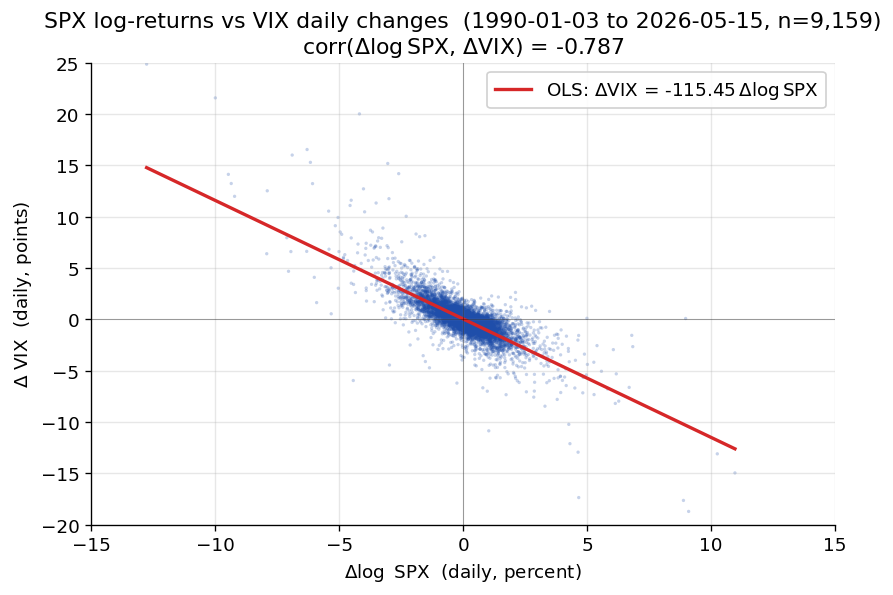
\includegraphics[keepaspectratio]{figures/ch10-vix-spx-scatter.png}}
\emph{Daily Δlog SPX vs Δ VIX scatter, full sample (n = 9,159).}

The scatter shows the linear relationship cleanly in the centre of the
distribution. Two features are visible in the tails: a sparse cluster of
points in the lower-right (large negative SPX moves producing very large
positive VIX moves) and a noticeably \emph{thinner} cluster in the
upper-left (large positive SPX moves producing more muted negative VIX
moves). That asymmetry is the subject of §B.5.

\subsection{B.4 Rolling correlation}\label{b.4-rolling-correlation}

The full-sample correlation hides substantial time variation. We compute
the 252-day rolling correlation between \(\Delta \log\) SPX and
\(\Delta\) VIX and report the summary statistics:

{\def\LTcaptype{none} % do not increment counter
\begin{longtable}[]{@{}lrl@{}}
\toprule\noalign{}
Statistic & Value & Date \\
\midrule\noalign{}
\endhead
\bottomrule\noalign{}
\endlastfoot
Mean & \(-0.770\) & --- \\
Median & \(-0.804\) & --- \\
Minimum (most negative) & \(-0.9626\) & 2020-03-16 \\
Maximum (least negative) & \(-0.4220\) & 1995-12-13 \\
2008 GFC peak negative & \(-0.868\) & 2008-10-31 \\
Feb 2018 Volmageddon & \(-0.791\) & 2018-02-28 \\
March 2020 COVID & \(-0.829\) & 2020-03-31 \\
\end{longtable}
}

\pandocbounded{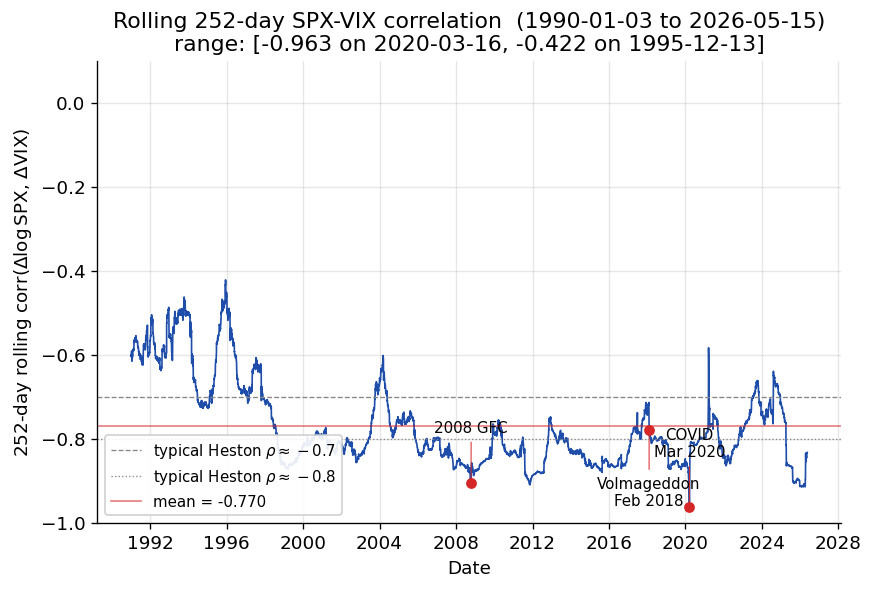
\includegraphics[keepaspectratio]{figures/ch10-vix-spx-rolling-corr.png}}
\emph{252-day rolling correlation of Δlog SPX and Δ VIX. Annotations
mark the major crises; the series never crosses zero.}

The series has three regimes. The early 1990s --- a low-volatility,
relatively shallow listed-option ecosystem --- show the weakest
correlations, with the all-time maximum of \(-0.4220\) in December 1995.
Through the 2000s and into the GFC, the correlation tightens
dramatically as index-option volumes grow, dealer hedging deepens, and
the SPX/VIX joint dynamic stabilises into the modern regime. The 2008
crisis pulls the rolling correlation toward \(-0.87\). The post-2010
regime is essentially flat around \(-0.80\) with sharp deepening into
crises: \(-0.96\) in March 2020 is the most negative print of the
sample.

Why does the correlation occasionally weaken? Three mechanisms are at
work. First, in extreme rallies --- particularly post-crisis bounces ---
forced de-grossing of short-vol positions pushes VIX up \emph{and} SPX
up together (cross-hedged unwinds), briefly reversing the usual sign of
the relationship and dragging the rolling correlation toward zero.
Second, vol-of-vol blowups (Aug 2015, Feb 2018) produce idiosyncratic
moves in VIX that are not fully explained by contemporaneous SPX moves
--- VIX has its own term-structure dynamics that decouple temporarily.
Third, structural breaks in dealer positioning (the post-Volmageddon ETP
unwind, the post-COVID dealer rebalancing) shift the gamma/vega flow
profile of the market and can change the local slope of the regression
for months at a time. The takeaway: the correlation is robustly negative
on average, but the daily slope is state-dependent in a way that no
constant-\(\rho\) model can capture.

\subsection{B.5 Asymmetric response}\label{b.5-asymmetric-response}

The headline summary correlation conceals a sharply asymmetric
relationship in the tails. Bucketing daily observations by the SPX
percent return and reporting the mean \(\Delta\) VIX in each bucket:

{\def\LTcaptype{none} % do not increment counter
\begin{longtable}[]{@{}lrr@{}}
\toprule\noalign{}
SPX bucket & n & mean \(\Delta\) VIX \\
\midrule\noalign{}
\endhead
\bottomrule\noalign{}
\endlastfoot
\(< -3\%\) & 107 & \(+6.44\) \\
\(-3\%\) to \(-2\%\) & 218 & \(+2.93\) \\
\(-2\%\) to \(-1\%\) & 792 & \(+1.62\) \\
\(-1\%\) to \(-0.5\%\) & 1014 & \(+0.74\) \\
\(-0.5\%\) to \(+0.5\%\) & 4476 & \(-0.07\) \\
\(+0.5\%\) to \(+1\%\) & 1326 & \(-0.70\) \\
\(+1\%\) to \(+2\%\) & 946 & \(-1.36\) \\
\(+2\%\) to \(+3\%\) & 187 & \(-2.28\) \\
\(> +3\%\) & 93 & \(-4.62\) \\
\end{longtable}
}

\pandocbounded{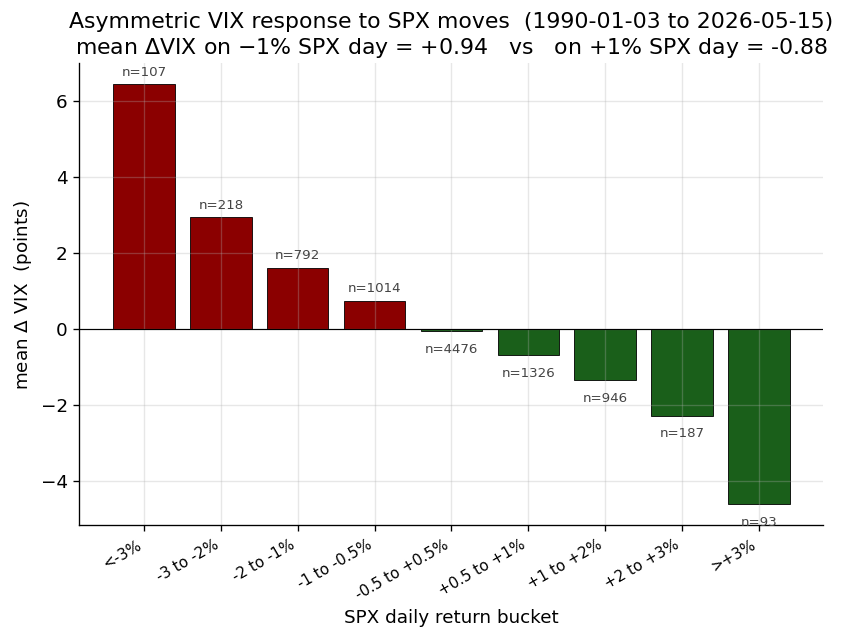
\includegraphics[keepaspectratio]{figures/ch10-vix-spx-asymmetry.png}}
\emph{Bucketed mean Δ VIX by SPX-return decile, 1990--2026. The
asymmetry between the two tails is the empirical fingerprint of jumps
and dealer-gamma dynamics that a pure-diffusion Heston cannot
reproduce.}

The inner buckets are nearly symmetric. SPX moves in \([-1.5\%,
-0.5\%]\) (n=1519) produce mean \(\Delta\) VIX of \(+0.943\); SPX moves
in \([+0.5\%, +1.5\%]\) (n=1992) produce mean \(\Delta\) VIX of
\(-0.882\). The ratio of magnitudes is \(0.943 / 0.882 = 1.07\) ---
within sampling error of perfect symmetry. The OLS regression of §B.3 is
calibrated mainly to these inner buckets and it does a good job there.

The tail buckets are not symmetric. SPX moves below \(-3\%\) (n=107)
produce mean \(\Delta\) VIX of \(+6.44\) (median \(+5.73\)); SPX moves
above \(+3\%\) (n=93) produce mean \(\Delta\) VIX of \(-4.62\). The
ratio of magnitudes --- \(6.44 / 4.62 = 1.39\) --- is well outside any
plausible sampling-error band; the tail-down move generates roughly 40\%
more VIX response than the tail-up move of equal magnitude. This is the
empirical leverage effect made unambiguous.

Two mechanisms drive it. The implied distribution embedded in the listed
SPX option strip is left-skewed; a \(-3\%\) move is a deeper quantile of
the risk-neutral density than a \(+3\%\) move, so it pushes the
at-the-money vol up by a larger multiple. And dealer positioning is
asymmetric: short-gamma dealer books hedge dynamically as SPX falls
(selling more vol-sensitive instruments and pushing implied vol up),
whereas in a rally the same books simply unwind existing hedges,
producing a more muted vol response. The asymmetry is structural and
persistent; it is visible in every post-1990 sub-sample we examined.

\subsection{\texorpdfstring{B.6 From daily correlation to Heston
\(\rho\)}{B.6 From daily correlation to Heston \textbackslash rho}}\label{b.6-from-daily-correlation-to-heston-rho}

VIX is a 30-day model-free implied volatility, not an instantaneous
variance. Heston \(\rho\) is the instantaneous correlation of the two
Brownians \(W^F\) and \(W^v\). The bridge between the two is not
algebraic but conceptual.

Take Itô differentials of the Heston spot-log and of \(\text{VIX}^2\)
--- the latter is, by the variance-swap representation, a linear
functional of the \emph{forward variance curve} \(m_T(t) =
\mathbb{E}_t[v_{t+T}]\), and the forward variance curve under Heston is
itself linear in \(v_t\) (see §10.8). It follows that \(\Delta
\text{VIX}^2_t\) is approximately proportional to \(\Delta v_t\), with a
proportionality constant that depends on \((\kappa, T)\) but not on the
realisation of \(v_t\). Hence \[
\operatorname{corr}\!\big(\mathrm{d}\log F,\;\mathrm{d}\text{VIX}^2\big)
\;\approx\;
\operatorname{corr}\!\big(\mathrm{d}\log F,\;\mathrm{d}v\big)
\;=\;\rho.
\] To a first approximation, the observed daily correlation between
\(\Delta \log\) SPX and \(\Delta \text{VIX}^2\) equals \(\rho\). There
is a Jensen-style nonlinearity because we actually observe \(\Delta\)
VIX (not \(\Delta \text{VIX}^2\)), but for the typical VIX level of
15--25 the linearisation
\(\Delta \text{VIX}^2 \approx 2\,\text{VIX}\,\Delta\text{VIX}\)
preserves the sign and approximate magnitude of the correlation.

Empirically, this means the observed daily \(-0.787\) implies a Heston
\(\rho\) in roughly \([-0.85,\,-0.70]\). Calibrated SPX Heston \(\rho\)
on listed-option surfaces typically lands in \([-0.85,\,-0.65]\),
varying with maturity (longer-dated tenors prefer the less negative end
as the smile decays) and with regime (post-crisis surfaces calibrate to
more negative \(\rho\) than pre-crisis surfaces). Weekly Euro Stoxx
(SX5E) surfaces calibrate to comparable \(\rho\) values --- the leverage
effect is a general equity-index phenomenon. Single-name equity surfaces
calibrate to flatter \(\rho\), typically \([-0.5,\,-0.3]\), because
individual company stocks lack the index-level joint-crash dynamic.

One final caveat about time aggregation. Daily-changes correlation
\emph{understates} instantaneous correlation. Over a day, both
\(\log F_t\) and \(v_t\) integrate many independent infinitesimal
innovations whose correlation is \(\rho\), but the realised daily
covariance also picks up cross-time-aggregation noise that biases the
correlation toward zero. The bias is small for \(|\rho|\) close to 1
(where the bound is tight) and larger for \(|\rho|\) near zero; for the
equity-index range of \(\rho \approx -0.8\) the bias is roughly
0.05--0.10. This is one reason calibrated \(\rho\) tends to be slightly
more negative than the realised daily correlation suggests.

\subsection{B.7 Caveats}\label{b.7-caveats}

A few things every practitioner should keep in mind when reading the
historical record.

The 30-day VIX horizon is not the instantaneous-vol object of the Heston
model. VIX prices a strip of options 23 to 37 calendar days out; the
model's \(v_t\) is the instantaneous variance at time \(t\). The mapping
is one-to-one (under Heston) but with a transformation involving
\(\kappa\) and the term structure, and any inference about \(\rho\) from
VIX must thread through that mapping.

VIX is a nontrivial functional of the entire option surface. When SPX
moves, the surface re-shapes --- strikes that were OTM are now ITM, the
at-the-money point moves, and the discrete weighting of the strike grid
changes. So \(\partial \text{VIX} / \partial \text{SPX}\) is not just
\(\partial\)(ATM vol)\(/\partial\) SPX; it includes sensitivity to the
entire surface's response to spot moves, and that sensitivity is itself
\(\rho\)-dependent in a model-consistent calculation. The realised
regression slope \(\hat\beta = -115\) is therefore a reduced-form
estimate that bundles together the model \(\rho\) and the surface's
spot-response geometry; it is not a pure \(\rho\) estimator.

Heston \(\rho\) in a calibration also absorbs effects that, strictly
speaking, are not correlations. The presence of unmodelled jumps in the
spot process biases the calibrated \(\rho\) toward more negative values,
because the model has no other parameter to fit the short-dated steep
skew that jumps would naturally produce. Bates (stochastic vol + jumps)
and rough vol models separate these contributions cleanly; in
pure-diffusion Heston they are mixed.

The asymmetric tail response of §B.5 is the most striking feature that
no pure-diffusion Heston can reproduce. A symmetric diffusion-driven
correlation must produce a symmetric mean-response function around zero
return (up to lognormal curvature, which is a much smaller effect than
the observed asymmetry). The factor-of-1.4 asymmetry in the \(>|3\%|\)
tail is a clean signature of jumps (Bates), rough volatility
(Bergomi-style rough Heston), or structural dealer-gamma effects that
lie outside the pure-diffusion-Heston modelling space. A practitioner
who fits Heston to a quiet surface and then runs it through a crisis
will find that the model under-predicts VIX spikes precisely because of
this missing tail asymmetry --- a fact worth knowing before sizing
positions on the strength of a Heston-implied risk number.

\subsection{B.8 Key takeaways}\label{b.8-key-takeaways}

\begin{itemize}
\tightlist
\item
  \textbf{Daily SPX-VIX correlation is strongly and persistently
  negative.}
  \(\operatorname{corr}(\Delta \log \text{SPX},\,\Delta \text{VIX}) = -0.787\)
  across 9,159 trading days from 1990 to 2026, and the 252-day rolling
  correlation has never been positive.
\item
  \textbf{The OLS slope is a useful trader's heuristic.} A 1\% drop in
  SPX corresponds on average to a \(+1.15\)-point move in VIX, and
  conversely for rallies. The intercept is economically negligible.
\item
  \textbf{The relationship deepens in crises.} Rolling correlation
  reaches \(-0.96\) in March 2020, \(-0.87\) in October 2008, \(-0.83\)
  in 2020 generally; it weakens to \(-0.42\) in the quiet mid-1990s and
  during forced-unwind episodes.
\item
  \textbf{The central response is symmetric, but the tails are not.}
  Inner-bucket asymmetry is \(\sim 7\%\); tail-bucket asymmetry exceeds
  \(\sim 40\%\). Down-3\% moves generate \(\sim 40\%\) larger VIX
  responses than up-3\% moves of equal magnitude.
\item
  \textbf{Daily correlation \(\approx -0.79\) implies Heston
  \(\rho \approx -0.7\) to \(-0.85\),} consistent with calibrated
  SPX-Heston values in the \([-0.85,\,-0.65]\) range. Daily-changes
  correlation slightly under-estimates instantaneous correlation due to
  time-aggregation bias.
\item
  \textbf{Single-name equities have flatter \(\rho\),} typically
  \([-0.5,\,-0.3]\), because individual stocks lack the index-level
  joint-crash dynamic.
\item
  \textbf{Pure-diffusion Heston cannot reproduce the tail asymmetry.}
  Capturing the \(>|3\%|\) asymmetric response requires jumps (Bates),
  rough vol, or explicit dealer-gamma modelling.
\item
  \textbf{\(\rho\) is the most information-dense parameter in
  equity-index Heston calibration.} It controls skew, joint-tail
  loadings, delta-vega cross-Greeks, and almost every risk-management
  decision a vol desk makes. The empirical record described here is what
  disciplines a sensible prior for it.
\end{itemize}

\begin{center}\rule{0.5\linewidth}{0.5pt}\end{center}

\emph{End of Chapter 10. Chapter 11 takes up calibration: how Heston
(and the rest of the model zoo) is fitted to market quotes day-to-day,
what makes a calibration well-posed, and the L-curve / regularisation
tradeoffs that decide whether a fit is usable for risk.}

\newpage

\chapter{Chapter 11 --- Calibration: Lattices, Short Rates, and the
Yield
Curve}\label{chapter-11-calibration-lattices-short-rates-and-the-yield-curve}

\section{11.1 FTAP on a Lattice}\label{ftap-on-a-lattice}

Pricing (Chapter 3--Chapter 5) maps parameters to prices; calibration
inverts that map. Given market quotes --- option prices, bond yields,
swap rates --- we pick the \(\mathbb{Q}\)-parameters that reproduce
them. The procedure is an \emph{inverse} problem with three classical
pathologies (non-existence, non-uniqueness, instability), each tamed by
a distinct tool (weighted least squares, regularisation, warm-start
smoothing). This chapter develops the apparatus on lattices and bond
curves; Chapter 12--Chapter 14 apply it to short-rate and stochastic-vol
models.

\subsection{11.1.1 Fundamental Theorem of Asset
Pricing}\label{fundamental-theorem-of-asset-pricing}

The first tool we need is the theorem that connects market data to model
structure. Its statement is deceptively simple, but every calibration
procedure in this chapter is, at bottom, a specialisation of this single
equation to a particular set of observed prices.

\textbf{FTAP (restated from Chapter 2 / Chapter 5).} \emph{No arbitrage}
\(\iff\) \emph{there exists an equivalent martingale measure}
\(\mathbb{Q} \sim \mathbb{P}\) \emph{such that for every traded asset}
\(X\):

\[
\frac{X_t}{B_t} \;=\; \mathbb{E}^{\mathbb{Q}}\!\left[\,\frac{X_T}{B_T}\,\Big|\,\mathcal{F}_t\,\right] \tag{11.1}
\]

where \(B_t\) is a traded numeraire with \(B_t > 0\) a.s. Any traded
asset normalised by the numeraire is a \(\mathbb{Q}\)-martingale.

Equation (11.1) is the most important equation in this chapter and one
of the most important in all of derivatives pricing. It is worth
committing to memory, not just as a formula but as a template. Every
calibration exercise we will perform is an instance of this template:
specify \(X\), specify \(B_t\), observe the left-hand side from market
data, parameterise the right-hand side in terms of model parameters, and
solve for the parameters. The specific forms will differ --- sometimes
the right-hand side is a simple discrete expectation, sometimes a
continuous-time expectation, sometimes a Gaussian integral --- but the
structure is universal.

Let us unpack each term carefully. The traded asset \(X\) can be a
stock, a bond, a futures contract, or a derivative --- the theorem is
agnostic about type, only that \(X\) is a price process quoted in a
market where self-financing trading is available. The numeraire \(B_t\)
is a reference asset against which all other prices are measured; it can
be the money-market account (so \(B_t = e^{rt}\) in a constant-rate
world, or \(\exp(\int_0^t r_u\,du)\) with stochastic rates), a
zero-coupon bond, a foreign currency, or any other strictly positive
traded process. The measure \(\mathbb{Q}\) depends on the choice of
numeraire: switching numeraires is equivalent to switching measures, as
developed canonically in Chapter 5. The conditional expectation
\(\mathbb{E}^{\mathbb{Q}}[\cdot\mid\mathcal{F}_t]\) is taken under
\(\mathbb{Q}\) and conditioned on the information available at time
\(t\).

The content of the theorem, stripped of formalism, is this: \emph{you
can price any claim by taking an expectation, provided you use the right
measure}. The right measure is the one under which normalised prices
become martingales. The right measure exists precisely when the market
admits no arbitrage. And --- crucially for us --- the right measure is
uniquely identified once you know enough about the market. Two
subtleties of the statement are worth flagging. First, FTAP in its
fullest generality requires care about integrability conditions,
stopping times, and the precise notion of ``no arbitrage'' (no free
lunch with vanishing risk is the right technical notion in continuous
time). These subtleties matter in pathological cases but are invisible
in the calibrations we perform. Second, the uniqueness of \(\mathbb{Q}\)
holds only in \emph{complete} markets, where every contingent claim can
be hedged. In incomplete markets (jumps, stochastic volatility without
traded volatility), there are many equivalent martingale measures, each
giving different prices for claims that cannot be hedged. Calibration in
incomplete markets picks \emph{one} of these measures --- the one that
matches the observed prices --- but the choice is a modelling decision,
not a mathematical inevitability.

\textbf{Reading FTAP as a calibration rule.} The theorem is often taught
as an existence statement, but operationally it is a \emph{constraint}.
For every tradable instrument whose \(t=0\) price we observe, (11.1)
gives one equation linking the unknown \(\mathbb{Q}\)-probabilities (and
unknown lattice parameters) to the observed price. With enough
independent instruments and enough unknowns, we get a determined (often
over-determined) system. Calibration is then nothing more than
\emph{solving this system} --- sometimes in closed form (as in §11.1.3
for the binomial moments, or §11.3 for bond lattice bootstrap) and
sometimes numerically (least squares against a basket of options). Think
of FTAP as giving you a \emph{coordinate system} on the space of
market-consistent models. Each observed price is a coordinate; each
unknown parameter is an axis. Calibration asks whether the observed
coordinates uniquely pick out a point on the axes. If they do, we are
done. If they underdetermine the point, we need more quotes. If they
overdetermine it, we solve in a least-squares sense and live with
residuals --- which, in practice, is almost always the situation.

A useful mental exercise: count equations and unknowns at the start of
any calibration problem. A single-factor Vasicek has four unknowns
(\(\kappa, \theta, \sigma, r_0\)). The short-rate observation gives one
equation directly. Each bond-price observation gives one more equation.
So four bond-price observations are needed to pin down four unknowns,
giving an exactly-determined system. In practice we observe far more
than four bonds --- maybe twenty at various maturities --- so the system
is over-determined, residuals are non-zero, and calibration is a
least-squares exercise. The Heston stochastic-volatility model has five
unknowns plus the initial spot; a liquid vanilla market provides
hundreds of quotes, so the system is massively over-determined. This
disparity between unknowns and observations is typical and is what makes
calibration a statistical, not algebraic, problem.

\textbf{Why numeraire invariance matters.} FTAP says the same underlying
prices satisfy (11.1) for many choices of numeraire, with
correspondingly different measures. This is not a redundancy; it is a
powerful tool. In equity derivatives the most common choice is the
money-market account, so \(\mathbb{Q}\) is the usual risk-neutral
measure. For interest-rate derivatives the \(T\)-forward measure
(numeraire \(= P_t(T)\)) simplifies expectations that would otherwise
involve stochastic discounting; Chapter 13 uses it pervasively. For FX
and quanto products, the domestic money market makes sense for some
payoffs and the foreign one for others. The practitioner picks the
numeraire that \emph{annihilates} the most inconvenient source of
randomness from the payoff, and the theorem guarantees the answer is the
same regardless.

\subsection{11.1.2 Single-Period Binomial
Lattice}\label{single-period-binomial-lattice}

Before we write down the lattice, it is worth pausing on why the
binomial structure is chosen rather than, say, a Gaussian step-size
distribution. The answer is pedagogical economy: the binomial model has
only two free parameters per step (the probability of up and the step
size), matching the two pieces of market data we want to extract (drift
and volatility). This symmetry between parameters and observations is
the cleanest possible setting for learning how moment matching works.
Once the binomial case is understood, extending to Gaussian, to
multinomial, or to jump-extended processes is a matter of adding
structure, not changing logic.

Start with one node \(A_{n-1}\) branching to two nodes over
\(\Delta t\):

\[
A_{n-1}\;\longrightarrow\;\begin{cases}
A_{n-1}\,e^{+c\sqrt{\Delta t}} & \text{(up)} \\
A_{n-1}\,e^{-c\sqrt{\Delta t}} & \text{(down)}
\end{cases}
\]

More compactly, introduce iid Bernoulli ticks \(x_1, x_2, \ldots\) with
\(\mathbb{P}(x_i = +1) = p\), \(\mathbb{P}(x_i = -1) = 1-p\). Then

\[
A_n \;=\; A_{n-1}\,e^{c\, x_n},\qquad x_i\stackrel{\text{iid}}{\sim}\text{Bernoulli}(\pm 1). \tag{11.2}
\]

The log-return \(\ln(A_n/A_{n-1}) = c\,x_n\) is \(\pm c\).

The parameter \(c\) has a clean interpretation: it is the magnitude of a
single-step log-return. If \(c = 0.02\) and \(\Delta t = 1\) day, then
on any given day the asset moves either up by roughly \(2\%\) or down by
roughly \(2\%\) (we use the exponential so that up-and-down produces
\(e^{c}e^{-c} = 1\), recovering the original level; multiplicative
symmetry matters here because log-returns are what sum across time). The
parameter \(p\) is the probability that the move is up; under the
physical measure \(\mathbb{P}\) this is tilted by the expected return,
under the risk-neutral measure \(\mathbb{Q}\) it is tilted only by the
cost of carry.

It is worth pausing on why log-returns, rather than arithmetic returns,
are the right quantity to model multiplicatively. Arithmetic returns do
not add across time: if an asset is up \(10\%\) today and up \(10\%\)
tomorrow, the two-day return is \(21\%\), not \(20\%\). Log-returns
\emph{do} add. This additivity is what makes log-returns amenable to the
Central Limit Theorem --- the sum of iid log-returns is approximately
Gaussian, while the product of iid gross returns is approximately
lognormal. The binomial model embraces this by writing each step as
\(S_n = S_{n-1}e^{c x_n}\) rather than \(S_n = S_{n-1}(1 + c x_n)\),
making the multi-step composition
\(S_N = S_0 e^{c(x_1 + x_2 + \cdots + x_N)}\) a clean exponential of the
summed shocks.

The Bernoulli shock \(x_i \in \{+1, -1\}\) is conventional --- it lets
us write each step as a scaled shock rather than a case split. In the
small-\(\Delta t\) limit, the sum of many iid Bernoulli shocks is
approximately Gaussian by the Central Limit Theorem, so the binomial
lattice converges to Brownian motion (Chapter 3). This is how the
binomial model recovers the Black--Scholes world in the limit, and why
the tree can be used as a discrete surrogate for continuous-time
pricing. It is also why moment matching gets the right answer: matching
two moments of a two-valued random variable fixes its distribution
completely, and the CLT does the rest. A practical aside: the binomial
tree as described here is \emph{recombining} --- the up-then-down path
and the down-then-up path land at the same price
\(S_0 e^{c}e^{-c} = S_0\). A recombining tree has \(n+1\) possible
terminal nodes after \(n\) steps (rather than \(2^n\)), which makes both
pricing and calibration computationally tractable.

\subsection{\texorpdfstring{11.1.3 Recovering \(p\) and \(c\) from
Observed
Data}{11.1.3 Recovering p and c from Observed Data}}\label{recovering-p-and-c-from-observed-data}

We want the parameters \((p, c)\) --- strictly, \((q, c)\) under
\(\mathbb{Q}\) --- to reflect what the market shows. Match the first two
moments of the log-return.

\textbf{Mean.} \[
\mathbb{E}^{\mathbb{P}}\!\left[\ln\!\tfrac{A_T}{A_0}\right] \;=\; \mathcal{N}\,c(2p-1) \;\equiv\; \hat\mu T \tag{11.3}
\]

where \(\mathcal{N} = T/\Delta t\) is the number of steps. The equation
should be parsed as follows. On each step, the log-return is \(c\,x_i\),
which has expectation \(c\mathbb{E}[x_i] = c(2p-1)\). Summing over
\(\mathcal{N}\) iid steps gives total log-return \(\mathcal{N}c(2p-1)\).
Equating this to \(\hat\mu T\) --- the observed physical drift --- gives
us our first calibration equation. Note the structural parallel with the
familiar one-factor Gaussian world: the total drift over \(T\) is linear
in \(T\), because drift is additive across independent steps.

Where does \(\hat\mu T\) come from in practice? There are several
sources, each with pitfalls. The most direct is historical return data:
compute the sample mean of daily log-returns and scale to annual. This
gives a point estimate of the physical drift, but the estimate is noisy
--- a one-year window of daily returns gives a drift estimate with
standard error of order \(\sigma/\sqrt{T}\), which for \(\sigma = 20\%\)
and \(T = 1\) year is \(20\%\) of the true drift. Historical drift
estimates are therefore nearly useless at short horizons and only
marginal at long ones; this is why risk-neutral measures are so much
more widely used in pricing applications --- the \(\mathbb{Q}\)-drift is
pinned down by the risk-free rate, which is observable with essentially
no noise.

\textbf{Variance.} \[
\mathbb{V}^{\mathbb{P}}\!\left[\ln\!\tfrac{A_T}{A_0}\right] \;=\; \mathcal{N}\,c^2\bigl(1 - (2p-1)^2\bigr) \;\equiv\; \sigma^2 T. \tag{11.4}
\]

Variance adds across iid steps, so total variance is \(\mathcal{N}\)
times the single-step variance. The single-step variance is
\(c^2\mathbb{V}[x_i]\) because \(c\) is a deterministic scale factor.
And
\(\mathbb{V}[x_i] = \mathbb{E}[x_i^2] - (\mathbb{E}[x_i])^2 = 1 - (2p-1)^2\),
using \(x_i^2 = 1\) with probability one. The quantity \((2p-1)^2\) is
small when \(p\) is near \(1/2\) --- which, as we will see, is the
regime relevant for small time-steps --- so \(\mathbb{V}[x_i]\approx 1\)
and the variance is approximately \(\mathcal{N}c^2\).

The variance \(\sigma^2 T\) is much easier to measure empirically than
the drift \(\hat\mu T\). The standard error of a realised variance
estimate scales as \(\sigma^2\sqrt{2/T}\) for large \(T\) and small
sampling intervals, so even a one-year history of daily returns gives a
variance estimate accurate to a few percent. This is why volatility
estimates from historical data are generally taken seriously in
practical pricing, while drift estimates are regarded with considerable
skepticism.

Equations (11.3) and (11.4) form a two-equation system in the two
unknowns \((p, c)\). The \(\mathbb{Q}\)-version is structurally
identical, only with \(\hat\mu\) replaced by the risk-neutral drift.
This two-for-two structure is a general feature of well-designed
moment-matching schemes: the number of free parameters equals the number
of moments matched, so the system is square and generically has a unique
solution.

\subsection{11.1.4 Small-Step Asymptotics}\label{small-step-asymptotics}

Write \(\sigma^2 T = \mathcal{N}\,c^2\bigl(1-(2p-1)^2\bigr)\). For small
\(\Delta t\), \((2p-1)^2 \ll 1\), so

\[
\sigma^2 T \;\approx\; \mathcal{N}\,c^2 \;=\; \frac{T}{\Delta t}\,c^2
\quad\Longrightarrow\quad \boxed{\;c \;\approx\; \sigma\sqrt{\Delta t}\;} \tag{11.5}
\]

Substituting into the mean equation \(\hat\mu T = c\,\mathcal{N}(2p-1)\)
gives \(2p - 1 \approx (\hat\mu/\sigma)\sqrt{\Delta t}\) and hence

\[
\boxed{\;p \;\approx\; \tfrac{1}{2}\!\left(1 + \tfrac{\hat\mu}{\sigma}\sqrt{\Delta t}\right)\;} \tag{11.6}
\]

This is the calibration of the physical probability \(p\). Under
\(\mathbb{Q}\), the same structural formula applies with \(\hat\mu\)
replaced by the drift that makes \(A_t/B_t\) a martingale
(e.g.~\(r - \tfrac12\sigma^2\) for a log-normal asset).

\textbf{Worked example.} Take \(\sigma = 0.20\), \(\hat\mu = 0.08\),
\(\Delta t = 1/252\). Then \(c = 0.20\sqrt{1/252} \approx 0.01260\) and
\(p \approx \tfrac12(1 + 0.4\sqrt{1/252}) \approx \tfrac12(1 + 0.0252) = 0.5126\).
An equity with \(20\%\) annualised volatility and \(8\%\) annualised
drift has, on a one-day step, about a \(1.26\%\) typical log-return
shock and a \(51.26\%\) probability of an up-move. The asymmetry between
up and down probabilities (just over one percentage point) is small
enough that if you looked at a few days of such returns you would see
what looks like a fair coin; the asymmetry only becomes clear when you
aggregate hundreds of days. Drift is small on short horizons and
dominates only over long ones, which is why the ``random walk''
intuition for short-term stock movements is approximately correct, and
why the drift-extractable information in historical returns is
notoriously noisy. The Sharpe ratio of \(0.08/0.20 = 0.4\) is typical
for equity indices --- equity risk premium divided by equity volatility
--- and reappears as the dominant signal in the calibration.

\textbf{Why the Brownian limit emerges.} The deeper reason moment
matching recovers the right continuous-time dynamics is the CLT. If on
each step we match the conditional mean and variance of log-returns to
\(\hat\mu\Delta t\) and \(\sigma^2\Delta t\) respectively, and the
shocks are independent, then the sum of \(\mathcal{N} = T/\Delta t\)
steps is a random variable with mean \(\hat\mu T\) and variance
\(\sigma^2 T\). As \(\Delta t \to 0\), the CLT guarantees this sum
converges in distribution to \(\mathcal{N}(\hat\mu T, \sigma^2 T)\) ---
which is exactly the log-return distribution of geometric Brownian
motion. The binomial tree is therefore not a separate model from
Black--Scholes; it is a discretisation that converges to the same limit,
provided the step sizes and probabilities are chosen (i.e.~calibrated)
in the way (11.5) and (11.6) prescribe. The scaling laws emerge from
dimensional analysis alone. Variance scales as \(\sigma^2 \Delta t\), so
the step size scales as \(\sigma \sqrt{\Delta t}\). The drift
contribution to the log-return scales as \(\hat\mu \Delta t\), and the
probability tilt must therefore scale as
\(\hat\mu \Delta t / (\sigma \sqrt{\Delta t}) = (\hat\mu/\sigma) \sqrt{\Delta t}\).

\textbf{From physical to risk-neutral: where the Sharpe ratio goes.}
Under \(\mathbb{Q}\), the drift that enters (11.6) is not \(\hat\mu\)
but the martingale drift --- for a stock paying no dividends in a
constant-rate world, \(r - \tfrac12\sigma^2\). The Sharpe ratio of the
\emph{risk premium} is therefore \((\hat\mu - r)/\sigma\), and this is
precisely the quantity that disappears when we pass to \(\mathbb{Q}\).
The formula structure is unchanged; the numerator in the tilt shifts
from \(\hat\mu\) to \(r - \tfrac12\sigma^2\), reflecting the replacement
of realised returns by risk-free returns. This is the lattice
incarnation of Girsanov's theorem (Chapter 5).

\textbf{Calibration as an inverse problem, restated.} The binomial
calibration is formally an \emph{exactly-determined} inverse problem,
not an ill-posed one. Two moments and two unknowns; a smooth, monotonic
map between moments and parameters as long as \(\sigma > 0\);
closed-form inversion via (11.5)--(11.6); straightforward stability. All
three of the usual pathologies of inverse problems --- non-existence,
non-uniqueness, instability --- are absent. This is why the binomial
case is pedagogically so useful: it lets us see the moment-matching
machinery at its cleanest, before the complications of real-world
calibration sink their teeth in. The other calibration problems in this
chapter and the next --- the bond-lattice bootstrap in §11.3, the
Vasicek yield-curve fit in Chapter 12, and the implied-vol surface fits
in Chapter 14 --- are all, to varying degrees, ill-posed, and each will
require one or more of the three remedies: weighted least squares,
regularisation, and cross-date smoothing.

\section{11.2 Change of Measure on Multinomial
Trees}\label{change-of-measure-on-multinomial-trees}

\subsection{11.2.1 Setup: Why Multinomial}\label{setup-why-multinomial}

Consider a richer lattice where a single node \(A_0\) branches to
multiple children (e.g.~three children \(A_1, B_1, C_1\) each with its
own sub-tree). Pricing under \(\mathbb{P}\) uses probabilities
\(\{p^A, p^B, p^C\}\); pricing under \(\mathbb{Q}\) uses
\(\{q^A, q^B, q^C\}\). We want to express the \(q\)'s in terms of the
\(p\)'s (and of observed price ratios).

Why bother with multinomial trees? The binomial tree is adequate for
simple equity options, but as soon as the state space has more than one
non-trivial dimension --- say, an equity \emph{and} an interest rate, or
an asset with both a continuous price component and a discrete jump
component --- we need lattices with more than two branches per step.
Trinomial trees also have a useful practical feature: the middle branch
allows the state to hold roughly constant, which is convenient for
modelling slow processes like mean-reverting interest rates. The
calibration logic below is cleanest in the binomial case but generalises
naturally.

A concrete example makes the case for multinomial lattices vivid.
Consider a callable bond: the issuer has the right to redeem the bond at
par on specified dates. Pricing this requires a short-rate lattice,
because the call decision depends on where rates go. If rates spike up,
the bond price drops, and the issuer has no incentive to call (they can
reborrow more cheaply by not calling). If rates drop, the bond price
rises, and the issuer calls to refinance. A binomial short-rate tree is
clumsy for this: the two branches move the state up or down with equal
probability, but mean-reverting rates typically have three economic
regimes --- rising, falling, or flat --- and the flat regime is where
most of the probability mass sits. A trinomial tree with up, middle, and
down branches captures this more naturally: the middle branch lets the
rate stay roughly where it is (consistent with a typical short-rate
half-life of several years), and the up and down branches capture the
tails. The price of a callable bond computed on a trinomial lattice
converges to the true continuous-time price faster than on a binomial
lattice with the same number of total nodes. Another example:
jump-diffusion equity models. If the underlying can either diffuse
continuously or jump to a distressed level, a single binomial branch
cannot capture both dynamics. A trinomial tree with ``up diffusion'',
``down diffusion'', and ``jump'' branches handles this cleanly, at the
cost of needing to calibrate three probabilities and three step sizes
rather than two.

The martingale identity (11.1) applied to numeraire-normalised values
gives, for each asset \(C\) (traded) and numeraire \(A\):

\[
\frac{C_0}{A_0} \;=\; q^A\,\frac{C_u}{A_u} + (1-q^A)\,\frac{C_d}{A_d} \tag{11.7}
\]

\[
\frac{C_0}{B_0} \;=\; q^B\,\frac{C_u}{B_u} + (1-q^B)\,\frac{C_d}{B_d} \tag{11.8}
\]

Here \(C_u, C_d\) are the values of \(C\) in the up and down states;
\(A_u, A_d, B_u, B_d\) are similarly the values of the two numeraire
candidates. The superscripts on \(q\) track \emph{which} numeraire the
measure is defined relative to --- \(\mathbb{Q}^A\) is the measure that
makes things a martingale in units of \(A\), and correspondingly for
\(\mathbb{Q}^B\). Different numeraires correspond to different
martingale measures, even though they price the same underlying claims;
Chapter 5 treated the continuous-time version of this relationship
exhaustively.

\subsection{\texorpdfstring{11.2.2 Solving for
\(q\)}{11.2.2 Solving for q}}\label{solving-for-q}

From (11.7): \[
q^A \;=\; \frac{\dfrac{C_0}{A_0} - \dfrac{C_d}{A_d}}{\dfrac{C_u}{A_u} - \dfrac{C_d}{A_d}}, \qquad q^B \;=\; \frac{\dfrac{C_0}{B_0} - \dfrac{C_d}{B_d}}{\dfrac{C_u}{B_u} - \dfrac{C_d}{B_d}}. \tag{11.9}
\]

Formulas (11.9) are simply the no-arbitrage pricing rule inverted. Read
them as follows: the risk-neutral probability of an up-move is the
``lever arm'' that makes the current normalised price \(C_0/A_0\) an
exact convex combination of the up- and down-state normalised prices. If
the current price is above the midpoint of the up and down
possibilities, \(q^A > 1/2\); if below, \(q^A < 1/2\). Crucially, if the
current price is \emph{outside} the range \([C_d/A_d, C_u/A_u]\), there
is no valid \(q^A \in [0,1]\) and the market is arbitrageable. This last
observation is why FTAP links the existence of \(\mathbb{Q}\) to the
absence of arbitrage: when an arbitrage exists, no consistent martingale
measure can reproduce the quotes.

A worked scenario makes this concrete. Suppose at time zero we observe
\(C_0 = 100\), \(A_0 = 98\), and at time \(\Delta t\) the two possible
states are \((C_u, A_u) = (110, 102)\) and \((C_d, A_d) = (90, 98)\).
The current ratio \(C_0/A_0 = 100/98 \approx 1.0204\); the up-state
ratio \(C_u/A_u = 110/102 \approx 1.0784\); the down-state ratio
\(C_d/A_d = 90/98 \approx 0.9184\). The current ratio sits comfortably
between the two future ratios, so the system is arbitrage-free, and we
compute
\(q^A = (1.0204 - 0.9184)/(1.0784 - 0.9184) = 0.1020/0.1600 = 0.6375\).
The \(\mathbb{Q}^A\)-probability of an up-move is \(63.75\%\); the
down-probability is \(36.25\%\). These probabilities are the market's
\emph{implicit} forward-looking assessment, under numeraire \(A\), of
the likelihood of each future state; they reflect both genuine
subjective probabilities and risk preferences, compressed into a single
no-arbitrage quantity. Now suppose instead that \(C_0\) is observed at
\(112\) rather than \(100\). The current ratio becomes
\(112/98 \approx 1.1429\), which is \emph{above} the up-state ratio
\(1.0784\). There is no \(q^A \in [0,1]\) that can reconcile this ---
the current price is higher than even the best future outcome, so an
arbitrageur could short \(C\), buy \(A\), and collect the spread. The
system is explicitly arbitrageable, and the calibration fails.
Calibration is not an optional step that improves the model --- it is an
\emph{arbitrage-detection} step. If calibration produces well-defined
parameters, the market is (locally) arbitrage-free; if it cannot, there
is a profitable trade sitting on the screen. In practice, this situation
is rare but not unheard of: stale quotes, manual data-entry errors, or
genuine market dislocations can all produce momentary violations. A
disciplined calibration system flags such quotes and either excludes
them or alerts a human operator.

\subsection{11.2.3 Radon--Nikodym on a Finite
Tree}\label{radonnikodym-on-a-finite-tree}

Express the same ratio \(C_0/B_0\) using numeraire \(A\) and convert:

\[
\frac{C_0}{B_0} \;=\; q^A\,\frac{A_0}{B_0}\cdot\frac{C_u}{A_u} + (1-q^A)\,\frac{A_0}{B_0}\cdot\frac{C_d}{A_d}
\]

Rewriting with \(B\)-ratios,

\[
\frac{C_0}{B_0} \;=\; \underbrace{q^A\,\frac{A_0}{B_0}\cdot\frac{B_u}{A_u}}_{>\,0}\cdot\frac{C_u}{B_u}
\;+\; \underbrace{(1-q^A)\,\frac{A_0}{B_0}\cdot\frac{B_d}{A_d}}_{>\,0}\cdot\frac{C_d}{B_d}. \tag{11.10}
\]

The key trick here is multiplying top and bottom by appropriate ratios
so that \(C\) appears normalised by \(B\) (as on the left) rather than
by \(A\). What matters is the \emph{form} of the result: \(C_0/B_0\) is
expressed as a convex combination of \(C_u/B_u\) and \(C_d/B_d\), with
new weights that differ from \(q^A\). Those new weights are the
\(\mathbb{Q}^B\)-probabilities, and they must equal \(q^B, 1-q^B\)
because (11.8) is the unique such representation. Compare term-by-term
with (11.8):

\[
q^B \;=\; q^A\cdot\frac{B_u/A_u}{B_0/A_0},
\qquad
(1-q^B) \;=\; (1-q^A)\cdot\frac{B_d/A_d}{B_0/A_0}. \tag{11.11}
\]

Consistency check. Summing the two pieces must give \(1\):

\[
q^B + (1-q^B) \;=\; \frac{A_0}{B_0}\!\left[\,q^A\,\frac{B_u}{A_u} + (1-q^A)\,\frac{B_d}{A_d}\right]
\;=\; \frac{A_0}{B_0}\cdot\frac{B_0}{A_0} \;=\; 1. \;\checkmark \tag{11.12}
\]

The bracket equals \(B_0/A_0\) because \(B/A\) is itself a
\(\mathbb{Q}^A\)-martingale. This consistency check is not a triviality;
it is the embodiment of the martingale property. If \(B/A\) is not a
\(\mathbb{Q}^A\)-martingale, the calculation fails --- the two new
weights do not sum to one, meaning there is no valid measure
\(\mathbb{Q}^B\). So the existence of an alternative pricing measure is
equivalent to the original one correctly pricing the \emph{new
numeraire} as a tradable asset.

Equations (11.11) are exactly the Radon--Nikodym density on the lattice:

\[
\boxed{\;
\frac{d\mathbb{Q}^B}{d\mathbb{Q}^A}(\omega) \;=\; \frac{B_\cdot(\omega)/B_0}{A_\cdot(\omega)/A_0}
\;}\tag{11.13}
\]

i.e.~the density is the \emph{ratio of numeraire-returns}. In shorthand,
writing \(\tilde A = A/A_0\) and \(\tilde B = B/B_0\):

\[
\frac{d\mathbb{Q}^B}{d\mathbb{Q}^A} \;=\; \frac{\tilde B}{\tilde A}. \tag{11.14}
\]

This is the discrete-time, finite-state incarnation of the
Radon--Nikodym derivative that Chapter 5 developed in continuous time.
Under \(\mathbb{Q}^A\) all prices are ``measured in units of \(A\)'';
switching numeraires to \(B\) is a relabelling of the unit, so scenarios
where \(B\) has over-performed \(A\) get up-weighted by their realised
relative return \(B_\cdot/A_\cdot\) (normalised by the \(t=0\) ratio so
that the density has mean one). The Radon--Nikodym density is therefore
a tradable object --- the ``relative performance'' of the two numeraires
--- not a mysterious abstraction. A probability measure has to integrate
to one, so any valid Radon--Nikodym density must have
\(\mathbb{E}^{\mathbb{Q}^A}[d\mathbb{Q}^B/d\mathbb{Q}^A] = 1\). From
(11.14): under \(\mathbb{Q}^A\),
\(\mathbb{E}^{\mathbb{Q}^A}[\tilde B_T / \tilde A_T] = \tilde B_0 / \tilde A_0 = 1\),
using that \(B/A\) is a \(\mathbb{Q}^A\)-martingale. So indeed the
density has mean one, and \(\mathbb{Q}^B\) is a well-defined probability
measure.

\textbf{Multi-step extension.} If the tree branches further at the
up-node (children with sub-probabilities \(q_u, r_u, \ldots\)) and
similarly at the down-node, each local change-of-measure is governed by
the same ratio. The overall change of measure from \(t=0\) to \(t=T\) is
the composition of all these local operations along every path. In the
continuous-time analogue (Chapter 5), this becomes a stochastic
exponential; in the discrete case it is a telescoping product of local
ratios. A calibrated tree can be diagnosed: at every node, one can check
that the local martingale property holds for each numeraire pair. If any
of these local checks fails, the calibration has introduced a local
arbitrage --- which is a bug. Production calibration systems routinely
run these checks as unit tests, catching implementation errors that
would otherwise manifest as mysterious mispricings downstream.

\pandocbounded{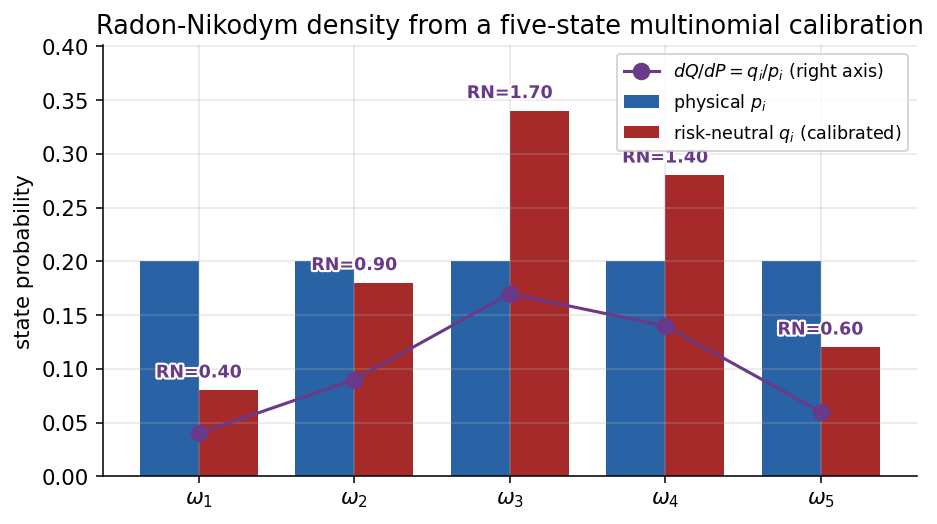
\includegraphics[keepaspectratio]{figures/ch11-rn-multinomial.png}}
\emph{Five-state discrete world: physical probabilities \(p_i\) (blue)
are uniform, while calibrated risk-neutral probabilities \(q_i\) (red)
tilt mass toward the central ``stress'' states that pricing data
implicates. The RN density \(dQ/dP = q_i/p_i\) (purple markers) records
that tilt state-by-state and is the discrete-tree analogue of the
continuous-time Girsanov density of Chapter 5.}

\subsection{11.2.4 Calibration as Optimisation: The Least-Squares
Setup}\label{calibration-as-optimisation-the-least-squares-setup}

Before turning to the interest-rate case, we pause to lay out the
calibration problem as it is actually formulated in practical systems.
Given \(N\) observed market instruments with prices
\(\{C_i^{\text{mkt}}\}_{i=1}^N\), a model with parameter vector
\(\Theta \in \mathbb{R}^d\), and a model pricing function
\(C_i^{\text{model}}(\Theta)\), the simplest calibration objective is

\[
\Theta^\star \;=\; \arg\min_\Theta \sum_{i=1}^N \bigl(C_i^{\text{model}}(\Theta) - C_i^{\text{mkt}}\bigr)^2. \tag{11.15}
\]

This is the ordinary least-squares (OLS) objective. Minimising (11.15)
gives the parameter vector that, on average, best reproduces the market
prices. The word ``best'' hides multitudes --- ``best'' in what sense,
under what weighting, with what penalty for over-fit --- and the next
several paragraphs unpack these choices.

The first and most important refinement is \emph{weighting}. Not all
market prices are equally informative. A deep in-the-money call option
that trades with a tight bid-ask is a tighter constraint on the model
than a deep out-of-the-money put trading with a wide bid-ask and small
absolute price. Equal weighting in price space treats them as equally
important; weighting each residual by the inverse bid-ask squared
downweights the noisy quote and lets the clean quote dominate. The
weighted least-squares objective is

\[
\Theta^\star \;=\; \arg\min_\Theta \sum_{i=1}^N w_i\bigl(C_i^{\text{model}}(\Theta) - C_i^{\text{mkt}}\bigr)^2, \tag{11.16}
\]

with \(w_i = 1/\text{spread}_i^2\) or some related quantity. The
algebraic form is the same as (11.15); the economic content is very
different.

A second common weighting scheme is \emph{vega weighting}. For options,
the natural trader-friendly quantity is implied volatility, not price.
Two options with the same implied volatility but different strikes have
very different prices, yet carry the same economic information.
Converting the least-squares fit from price space to implied-volatility
space is equivalent to weighting each price residual by
\(1/\text{vega}_i\), because vega
\(= \partial C/\partial \sigma_{\text{imp}}\) is exactly the local
conversion factor. The vega-weighted objective is

\[
\Theta^\star \;=\; \arg\min_\Theta \sum_{i=1}^N \frac{\bigl(C_i^{\text{model}}(\Theta) - C_i^{\text{mkt}}\bigr)^2}{\text{vega}_i^2}, \tag{11.17}
\]

which is equivalent (to first order, near the market-implied volatility)
to

\[
\Theta^\star \;=\; \arg\min_\Theta \sum_{i=1}^N \bigl(\sigma_i^{\text{model}}(\Theta) - \sigma_i^{\text{imp,mkt}}\bigr)^2. \tag{11.18}
\]

Vega is the option's sensitivity to implied volatility; near-the-money
options have high vega, deep OTM options have low vega. In price space,
a \(1\%\) error in an at-the-money price might correspond to a
\(0.1\)-vol error, while a \(1\%\) error in a deep OTM price might
correspond to a \(5\)-vol error. An unweighted fit would treat these as
equally bad; a vega-weighted fit treats the deep OTM error as \(50\)
times worse --- as a trader quoting in vol space would insist. A subtle
caveat: vega-weighting is a \emph{linearisation}; it breaks down for
very deep OTM options where the vega is vanishingly small and a literal
\(1/\text{vega}^2\) weight gives that strike enormous, usually spurious,
importance. A practical weighting scheme caps the weight,
\(w_i = \min(1/\text{vega}_i^2, w_{\max})\), or combines vega and spread
weighting via a harmonic mean. Tuning these caps is part of the craft of
building a robust calibration.

\subsection{11.2.5 Global vs Local Minima}\label{global-vs-local-minima}

The objective function (11.15) is, in general, a non-convex function of
the parameters \(\Theta\). For the binomial lattice it happens to be
quadratic (the moment-matching equations are linear in parameters after
log-transformation), but for more general models --- stochastic
volatility, jump diffusion, multi-factor rates --- the landscape has
multiple local minima. Which minimum the optimiser finds depends on
where it starts. This is a serious practical concern. An equity trader
who runs a stochastic-volatility model on Monday morning and gets
parameters \((\kappa = 2, \theta = 0.04, \alpha = 0.3, \rho = -0.7)\)
may rerun the same calibration on Tuesday with yesterday's minimum as a
starting point and get
\((\kappa = 2.1, \theta = 0.041, \alpha = 0.31, \rho = -0.71)\) --- a
small, economically sensible shift. But if the starting point is reset
to a default every day, Tuesday's run might find a completely different
local minimum, say
\((\kappa = 0.5, \theta = 0.06, \alpha = 0.5, \rho = -0.9)\), with
similar fit quality but very different economic implications. The two
parameter vectors produce nearly identical prices on the calibration
basket but very different prices on instruments \emph{outside} the
basket. If the bank uses the Monday parameters to price exotics on
Tuesday but recalibrates for the blotter, the exotics will be valued one
way while the hedging positions use a different calibration --- a recipe
for P\&L surprise.

The standard defenses against this problem are:

\begin{enumerate}
\def\labelenumi{\arabic{enumi}.}
\tightlist
\item
  \textbf{Warm starts.} Always initialise today's calibration from
  yesterday's minimum. This enforces continuity across dates and
  typically keeps the optimiser in the same local basin even if another
  basin is marginally deeper. The cost is that the calibration may
  become ``stuck'' in a stale minimum if the market has genuinely moved
  to a new regime; the remedy is to add periodic cold starts to check
  for regime shifts.
\item
  \textbf{Multi-start optimisation.} Run the optimiser from several
  starting points (a small random grid, or structured starts from
  economically plausible prior values) and take the best. If multiple
  starts converge to distinct minima of comparable depth, the problem is
  flagged as non-identifiable and a human operator is consulted.
\item
  \textbf{Global optimisation methods.} Use algorithms designed to
  escape local minima --- simulated annealing, differential evolution,
  genetic algorithms, basin-hopping. These are slower than
  gradient-based local methods but more reliably find global minima.
\item
  \textbf{Problem reformulation.} Often the landscape can be smoothed by
  changing variables. Calibrating Heston (Chapter 10) in
  \((\kappa, \theta, \alpha, v_0, \rho)\) is notoriously multimodal;
  reparameterising in terms of more orthogonal quantities ---
  at-the-money variance, skew, curvature, mean-reversion speed --- can
  make the landscape nearly convex. This is sometimes called
  ``calibrating in the right coordinates''.
\end{enumerate}

\subsection{11.2.6 Numerical Methods}\label{numerical-methods}

The optimisation problems above are nonlinear least-squares in a
moderate-dimensional space. Several algorithmic families are in common
use. \emph{Nelder--Mead} maintains a simplex of \(d+1\) points and
iteratively reflects, expands, contracts, and shrinks it; it requires
only function evaluations (no gradients), so it is robust to objectives
that are noisy, discontinuous, or expensive to differentiate, at the
cost of slow convergence. \emph{Levenberg--Marquardt} is the gold
standard for nonlinear least-squares: it exploits the sum-of-squares
structure to approximate the Hessian from Jacobians alone, and blends
Gauss--Newton with gradient-descent via a damping parameter \(\lambda\).
It typically converges in tens of iterations on well-posed problems; for
implied-vol-surface fits with \(N \sim 100\) instruments and
\(d \sim 5\) parameters, it converges in milliseconds. \emph{BFGS} and
\emph{L-BFGS} are quasi-Newton methods building up a Hessian
approximation iteratively --- the full version for moderate \(d\), the
limited-memory version for thousands of parameters. \emph{Differential
evolution} and related global methods maintain a population of candidate
parameter vectors and evolve them via mutation, crossover, and
selection; they are slower (seconds to minutes) but reliably find global
minima.

\textbf{Hybrid strategies.} A production calibration system rarely uses
a single method. A typical setup: start with a coarse
differential-evolution search to find a plausible global minimum; refine
with Levenberg--Marquardt for tight local convergence; verify stability
with a Nelder--Mead polish. Practical runtime targets: a single-factor
rates model against 20 bond quotes under \(10\) ms; Heston against
\(100\) vanilla options under \(100\) ms; a multi-factor Libor market
model against \(500\) caplet/swaption quotes under \(10\) seconds.
Faster is always better, but stability and correctness trump speed by a
wide margin in production.

\subsection{11.2.7 Regularisation and
Well-Posedness}\label{regularisation-and-well-posedness}

When the calibration problem is under-determined --- more parameters
than informative observations, or observations that leave a sloppy
direction unpinned --- regularisation adds a penalty term to the
objective function:

\[
\Theta^\star \;=\; \arg\min_\Theta \Bigl[\sum_i w_i\bigl(C_i^{\text{model}}(\Theta) - C_i^{\text{mkt}}\bigr)^2 + \lambda \,\mathcal{R}(\Theta)\Bigr]. \tag{11.19}
\]

The penalty \(\mathcal{R}(\Theta)\) encodes prior knowledge: smoothness
(\(\|\nabla^2 \Theta\|^2\) for curve fits), proximity to a historical
mean (\(\|\Theta - \Theta_{\text{prior}}\|^2\)), sparsity
(\(\|\Theta\|_1\)), or any other property the modeller wants to
encourage. The weight \(\lambda\) controls how much regularisation is
applied: small \(\lambda\) trusts the data, large \(\lambda\) trusts the
prior. Choosing \(\lambda\) is itself a subproblem, usually handled by
cross-validation (try several \(\lambda\) values and pick the one that
minimises out-of-sample error) or by Bayesian hierarchical modelling
(treat \(\lambda\) as a hyperparameter to be integrated over).

The Bayesian interpretation of regularisation is worth holding in mind.
A penalty \(\|\Theta - \Theta_{\text{prior}}\|^2\) is equivalent to a
Gaussian prior on \(\Theta\) centred at \(\Theta_{\text{prior}}\); a
penalty \(\|\Theta\|_1\) is equivalent to a Laplace prior at zero; a
penalty \(\|\nabla^2 \Theta\|^2\) encodes a prior that parameter values
change smoothly along some ordering (useful for term-structure
calibration where we expect neighbouring maturities to have similar
parameters). Regularisation is the frequentist's way of sneaking
Bayesian priors into a point-estimate framework.

\textbf{The fit-vs-extrapolation tradeoff.} Strong regularisation
(\(\lambda\) large) produces parameter estimates that are close to the
prior, insensitive to the data, and therefore stable but potentially
biased. Weak regularisation (\(\lambda\) small) produces parameter
estimates that fit the data tightly, sensitive to every wiggle, and
therefore unbiased in expectation but high-variance in any given run.

\pandocbounded{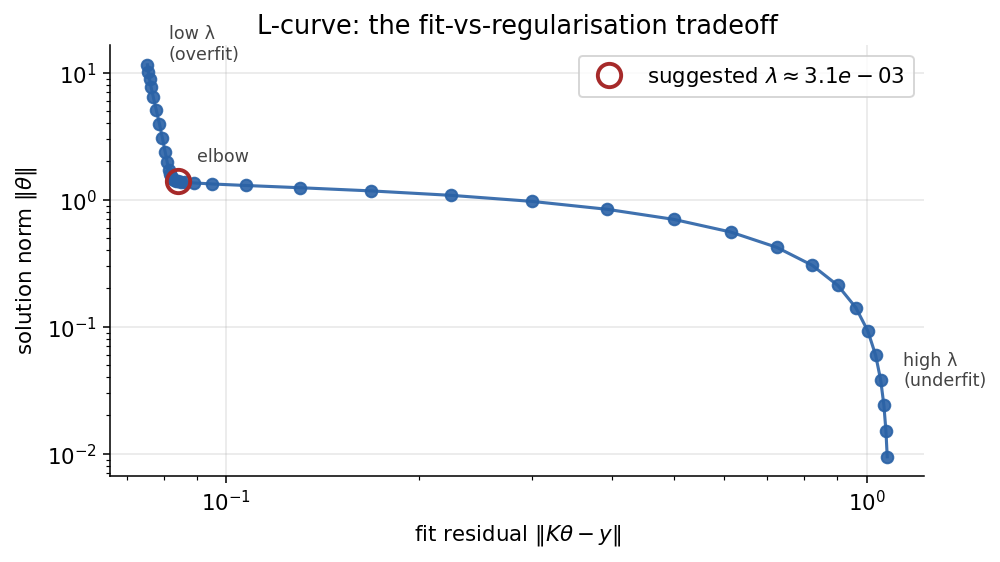
\includegraphics[keepaspectratio]{figures/ch11-lcurve.png}}
\emph{L-curve diagnostic for a Tikhonov-regularised linear inverse
problem. Each point is one value of \(\lambda\); the corner (elbow,
marked) is the classical heuristic choice --- the regularisation
strength beyond which further stiffening raises residual without
lowering solution norm. Small-\(\lambda\) end: data-fitting, overfit
regime. Large-\(\lambda\) end: prior-dominated, underfit regime.} The
sweet spot depends on the application: a conservatively-marked book
wants stability (high \(\lambda\)); an aggressive trading book wants
responsiveness (low \(\lambda\)). There is no universal right answer,
and the choice is part of the desk's risk-appetite statement. A related
perspective: in-sample fit is a strictly decreasing function of
\(\lambda\) (regularisation makes the model stiffer, so it fits the
training data less well), while out-of-sample fit is typically U-shaped
(zero regularisation overfits, infinite regularisation underfits, and
the optimum is somewhere in between). Cross-validation finds this
optimum empirically.

\pandocbounded{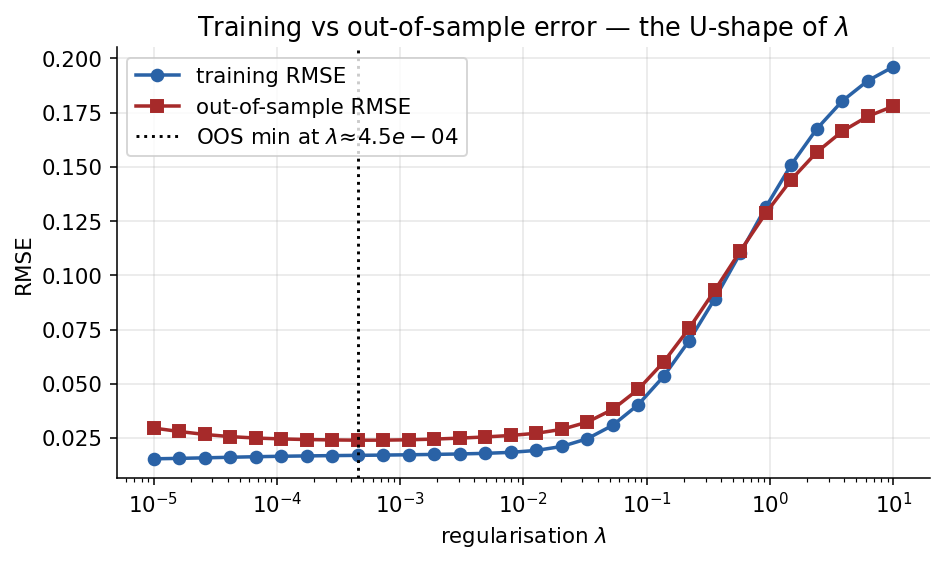
\includegraphics[keepaspectratio]{figures/ch11-oos-validation.png}}
\emph{The U-shape of out-of-sample error (red) in \(\lambda\) contrasts
with the monotone rise of training error (blue). Small \(\lambda\)
overfits --- training error shrinks but OOS error spikes; large
\(\lambda\) underfits --- both errors rise. The optimum \(\lambda\) is
the OOS minimiser, found in practice by cross-validation.}

\textbf{Out-of-sample stability.} A calibrated model's in-sample
performance is tautological: by construction, the model matches its
calibration instruments to within the optimiser's tolerance. The real
test is \emph{out-of-sample}: does the model correctly price instruments
that were not in the calibration basket? There are two flavours of
out-of-sample test. The first is \emph{cross-sectional}: calibrate using
a subset of instruments (say, vanilla options at strikes
\(K_1, \ldots, K_{10}\)) and check the fit on a held-out strike
\(K_{11}\). If the model is correctly specified and the calibration is
well-regularised, the held-out fit should be nearly as good as the
in-sample fit. If the held-out fit is markedly worse, the model is
overfitting --- squeezing the in-sample error to zero at the cost of
off-sample generalisation. The second flavour is \emph{temporal}:
calibrate today, price a hold-out instrument today, then hold the model
parameters fixed and re-price the same instrument tomorrow. Compare
against tomorrow's market price. If parameters are stable day-to-day,
the deviation should be small; if parameters wobble, the deviation will
be dominated by recalibration noise rather than genuine market movement.
Both tests are routinely neglected in practice --- the in-sample fit is
visually appealing and easy to report to management, while out-of-sample
tests require more infrastructure. But any model going into production
should be subjected to both.

\section{11.3 Short-Rate Bootstrap on a Bond
Lattice}\label{short-rate-bootstrap-on-a-bond-lattice}

\subsection{11.3.1 Zero-Coupon Bonds as Calibration
Instruments}\label{zero-coupon-bonds-as-calibration-instruments}

Let \(P_t(T)\) denote the zero-coupon bond price at time \(t\) paying
\(1\) at maturity \(T\). On a short-rate lattice
\(\{r_0, r_{11}, r_{22}, \ldots\}\) (a recombining tree of realised
short rates indexed by time step and node-within-step), the one-period
bond satisfies

\[
P_0(1) \;=\; \frac{1}{1 + r_0}
\qquad\Longleftrightarrow\qquad
r_0 \;=\; \frac{1}{P_0(1)} - 1. \tag{11.20}
\]

(Convention note. The discount factor \(1/(1 + r_t)\) used throughout
§11.3 is the \emph{simple-compounding} version; elsewhere in the guide
--- and in the CRR lattice conventions of §11.1.2 --- we use exponential
discounting \(e^{-r_t\,\Delta t}\). The two agree to leading order in
\(\Delta t\) ---
\(1/(1+r_t\Delta t) = e^{-r_t\Delta t}(1 + O(\Delta t^2))\) --- so the
sequential-bootstrapping arithmetic below is unaffected at the orders of
accuracy we care about. We keep the simple-compounding form in §11.3
because it matches the market quoting convention for short-dated zero
coupons, which is how the bootstrap inputs are usually presented in
practice.)

Two-period bonds satisfy, at each child node,

\[
P_{11}(2) \;=\; \frac{1}{1 + r_{11}},\qquad P_{22}(2) \;=\; \frac{1}{1 + r_{22}}. \tag{11.21}
\]

Rolling back to \(t=0\) under the risk-neutral measure \(\mathbb{Q}\):

\[
P_0(2) \;=\; \frac{1}{1 + r_0}\!\left[\,q\,P_{11}(2) + (1-q)\,P_{22}(2)\right]. \tag{11.22}
\]

Zero-coupon bonds are the canonical calibration instruments for
interest-rate models because their payoffs are entirely deterministic
--- they pay \(1\) at maturity, with no optionality to muddy the waters.
Any uncertainty in the bond's current price therefore comes purely from
the uncertainty of the path of short rates between now and maturity.
Observing \(P_0(T)\) for many maturities pins down the \emph{term
structure} of the short-rate risk-neutral dynamics, which is exactly
what a short-rate model needs.

A useful intuition: a zero-coupon bond's yield is the constant rate at
which, if the future were certain, the bond would compound to face
value. When the future is uncertain, the yield is the
\emph{certainty-equivalent} rate --- the deterministic rate that, if
applied over the bond's life, would produce the same discounted payoff
as the actual stochastic rate path. Because Jensen's inequality makes
the expectation of the discount factor bigger than the discount factor
at the expected rate, the certainty-equivalent yield is slightly below
the expected average rate. This is the convexity correction that Chapter
12 derives rigorously for the Vasicek model; at this stage, the point is
only that every bond quote is a statement about the certainty-equivalent
of a stochastic path, and each independent maturity provides one
independent equation relating parameters to data.

Equation (11.20) is the simplest imaginable calibration equation:
knowing today's one-period bond price directly gives today's short rate.
Equation (11.21) is equally simple, but at the next time step --- at
each possible future short-rate state, the corresponding one-period bond
price is fixed. The interesting work happens in (11.22), which enforces
no-arbitrage between the \(t=0\) quote and the \(t=\Delta t\) states.
Here both \(q\) and the short-rate states are, in principle, unknowns.
The progression from (11.20) to (11.22) illustrates a key feature of
tree-based calibration: each successive equation adds information about
one more future time slice. (11.20) pins the \(t=0\) node; (11.22) pins
the \(t=\Delta t\) node (given a vol input); the analogous three-step
equation pins \(t=2\Delta t\); and so on. The calibration proceeds
recursively, one time slice at a time, building up a discrete
yield-curve-consistent tree. This is the same recursive logic as in the
Black--Derman--Toy (BDT) model or the Ho--Lee model --- both of which
are, at bottom, schemes for backing out tree parameters from bond-price
ratios, one time slice at a time, in a way that exactly reproduces the
observed yield curve. Chapter 12 develops the continuous-time limits of
these constructions; here we focus on the discrete bootstrap.

\subsection{\texorpdfstring{11.3.2 Recovering \(q\) and the Short
Rates}{11.3.2 Recovering q and the Short Rates}}\label{recovering-q-and-the-short-rates}

Given \(P_0(1)\) (one-year bond price) and \(P_0(2)\) (two-year bond
price), plus a volatility assumption that fixes the spread between
\(r_{11}\) and \(r_{22}\)
(e.g.~\(r_{22} = r_{11}\,e^{-2c\sqrt{\Delta t}}\)), equations
(11.20)--(11.22) give a system of two equations in \((q, r_{11})\) that
can be solved numerically. A simple illustrative case takes \(q = 1/2\),
which then delivers \(r_{11}\) explicitly from (11.22): \(r_{11}\) is
chosen such that \(\frac{1}{1+r_{11}}\) and \(\frac{1}{1+r_{22}}\),
mixed half-half, reproduce \(P_0(2)(1+r_0)\). In practice the tree is
built \emph{sequentially} from the observed yield curve
\(\{P_0(1), P_0(2), P_0(3), \ldots\}\) and a term structure of
volatilities --- at each new level we solve for the fresh short-rate
node that reprices the newly observed bond.

\textbf{Why sequential construction works.} The recursive nature of bond
pricing --- today's bond price is a discount of a convex combination of
tomorrow's bond prices, which are themselves discounts of further-future
bond prices --- means calibration can be done layer by layer. Once the
\(t=0\) node is pinned down (trivially from (11.20)), the \(t=\Delta t\)
layer is pinned down by the two-period bond (11.22) plus a volatility
input. The three-period bond \(P_0(3)\) then pins down the
\(t=2\Delta t\) layer, and so on. This is the classical Ho--Lee /
Hull--White / BDT construction, and it produces a tree that exactly
reproduces the input yield curve by design. The tree is then said to be
\emph{bootstrapped}.

\textbf{The role of the volatility input.} Without a volatility input,
the system is underdetermined: for a binomial tree at step
\(t=\Delta t\) there are two rate states \(r_{11}, r_{22}\) and a
transition probability \(q\), but only one bond quote \(P_0(2)\) ---
three unknowns and one equation. We need extra information to pin down
the spread between \(r_{11}\) and \(r_{22}\). In practice this comes
from one of three sources: (i) an explicit volatility assumption
(e.g.~``short rates have \(1.2\%\) annualised vol''), (ii) a market
quote on an interest-rate option (caplet, swaption) whose price encodes
the volatility, or (iii) a direct measurement of historical volatility
of the short rate. Each source gives a different calibration flavour;
market-consistency purists prefer (ii) because it is the only source
that is consistent with tradable instruments.

\textbf{Interpolation vs extrapolation.} The bootstrapped tree
reproduces the calibration instruments \emph{exactly}. That is a
property of construction, not a property of truth. For maturities
\emph{within} the calibration set, the model is interpolating between
observed quotes, and we are entitled to a measured trust in its outputs.
For maturities \emph{beyond} the calibration set --- or for instruments
that depend on joint dynamics we have not fit --- the model is
extrapolating, and its outputs are only as good as the extrapolation.
This distinction matters enormously in practice: a Vasicek fit
calibrated to the 1-month, 3-month, 6-month, and 1-year bonds will
reproduce those four quotes exactly (if it has four free parameters) but
may produce wildly different 30-year yields from a Vasicek fit
calibrated to 10-year, 20-year, and 30-year bonds. Both fits are
``correct'' in the interpolating region; neither is trustworthy in the
extrapolating region.

The practical implication is that a calibration's range of
trustworthiness is determined by its calibration set, not by the model's
parametric form. A Vasicek model calibrated to short maturities will
give short-maturity answers you can trust, but its long-maturity
extrapolation is model-dependent in ways the short-maturity data cannot
validate. Similarly, an implied-vol surface calibrated to near-the-money
strikes will give near-the-money prices you can trust, but deep
out-of-the-money extrapolation is driven by the model's tail behaviour,
which the near-the-money data does not constrain. Recognising and
reporting this range-of-trustworthiness is a hallmark of mature
modelling practice. It is often the first question a risk committee asks
before approving the use of a model: ``for what range of instruments and
market conditions has this model been validated?''

\begin{quote}
\textbf{Key point.} The tree expectation is taken under the
\emph{bond-numeraire} risk-neutral measure, i.e.~payoffs are discounted
by \(\prod(1+r_{m-1}\Delta t)\) along each path, which is the discrete
analogue of discounting by \(\exp(\int_0^T r_u\,du)\) under
\(\mathbb{Q}^M\). Chapter 5 formalised this numeraire-by-numeraire
correspondence in continuous time.
\end{quote}

\pandocbounded{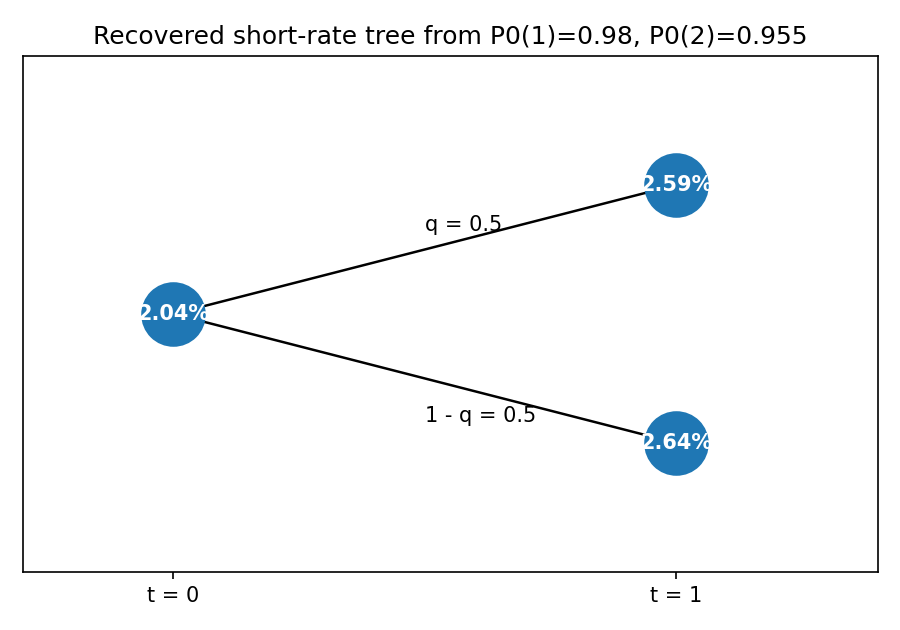
\includegraphics[keepaspectratio]{figures/ch11-bond-tree-recover.png}}
\emph{Recovered short-rate tree --- given two bond quotes and a
volatility spread \(c\), the pair \((r_0, r_{11})\) is pinned down by
the no-arbitrage mixing relation (11.22).}

\pandocbounded{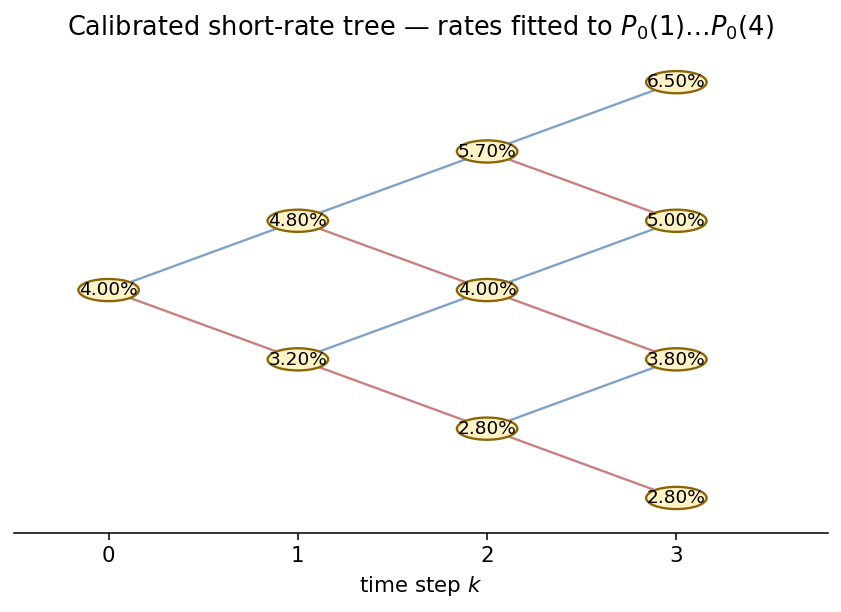
\includegraphics[keepaspectratio]{figures/ch11-calibrated-tree.png}}
\emph{Layered extension: a four-step recombining short-rate tree whose
node rates have been bootstrapped from a sequence of bond quotes
\(P_0(1), \ldots, P_0(4)\) and a term structure of volatilities. Each
time-slice is pinned down by the freshly observed bond; the tree is
arbitrage-free by construction and exactly reprices its calibration
instruments.}

\pandocbounded{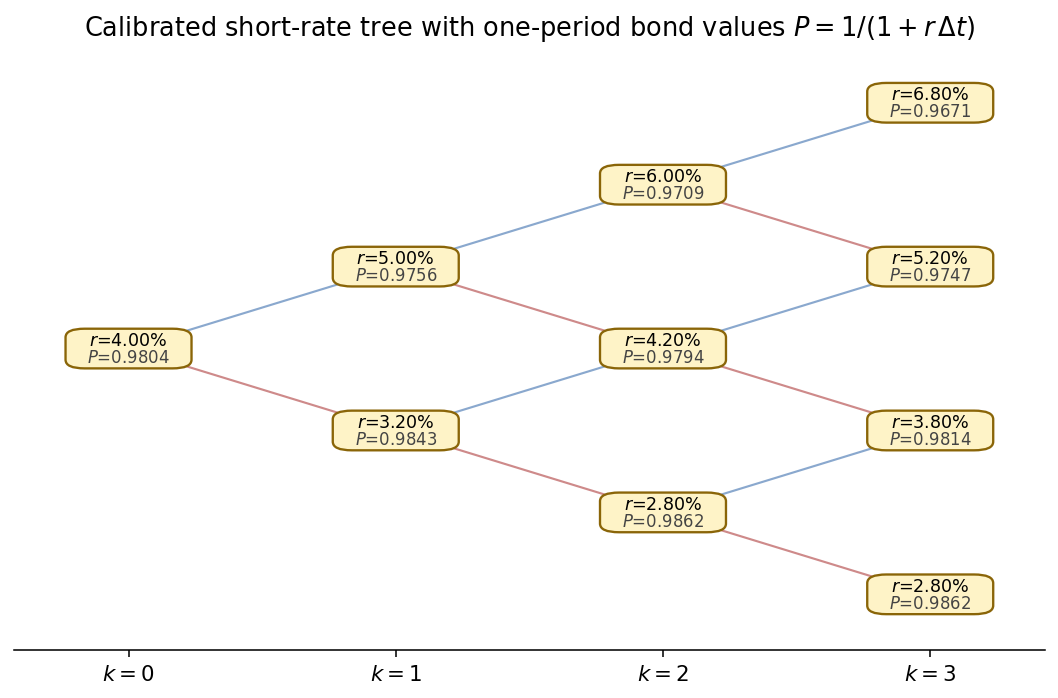
\includegraphics[keepaspectratio]{figures/ch11-bond-lattice.png}}
\emph{The same calibrated tree, now annotated with the implied
one-period bond value \(P=1/(1+r\,\Delta t)\) at each node. This is the
object pricing routines roll back over: each step multiplies the
weighted average of child-node bond values by the parent's discount
factor, and matching this roll-back to the observed \(P_0(T)\) quotes
pins down the calibration.}

\subsection{11.3.3 Bid-Ask, Stale Quotes, and Data
Hygiene}\label{bid-ask-stale-quotes-and-data-hygiene}

\textbf{Bid-ask spreads and stale quotes.} In real markets, \(P_0(T)\)
is not a single number but a bid-ask pair
\((P^{\text{bid}}, P^{\text{ask}})\), and between transactions the quote
may be stale --- indicating only an indicative level rather than a
tradable price. Calibration that targets an arbitrary mid-price within
the bid-ask can give nonsensical parameter wobble: if the spread is
\(2\) basis points and calibration is trying to fit to \(0.1\) basis
point precision, the resulting parameters will move randomly within a
band set by the spread even when no economic information has changed. A
disciplined calibration treats the bid-ask as a confidence interval: fit
the mid, but accept any parameters that produce model prices inside the
bid-ask as equally valid. Stale quotes are even more pernicious; if a
bond hasn't traded in a week, its ``price'' is an echo, and calibrating
to it pollutes the rest of the curve.

An instructive exercise is to simulate the impact of bid-ask noise on a
calibrated parameter vector. Take a realistic fit --- say, a Vasicek
calibration to ten bond quotes --- and perturb each input yield by a
uniform random amount in \([-\text{spread}/2, +\text{spread}/2]\). Rerun
the calibration for many such perturbations, and plot the resulting
distribution of calibrated parameters. If the spread is \(2\) basis
points and the parameter distribution spans \(10\%\) of the point
estimate, the calibration is reporting precision far in excess of what
the data supports. A well-calibrated system's reported precision should
roughly match the width of this simulated perturbation distribution ---
any tighter is over-confidence, any looser is under-utilisation of the
data. This exercise is worth running periodically as a calibration
sanity check; it catches both model misspecification and implementation
bugs that compress or inflate the reported precision artificially.

\textbf{Liquidity weighting.} A related practical refinement: weight
each quote in the calibration objective by its liquidity, proxied by
trading volume or quote frequency. A quote for an on-the-run 10-year
Treasury is updated every second and traded millions of times a day; a
quote for an off-the-run 17-year Treasury may be updated only a few
times a day and traded in small size. Both quotes are nominally ``mid
prices'', but the 10-year mid is a much more trustworthy signal.
Weighting by volume (or by the inverse of some proxy for staleness) is
one way to ensure the calibration reflects the information in the market
rather than the information in yesterday's stale print. A common scheme:
weight each residual by the instrument's proportion of recent trading
volume, normalised so that the weights sum to one.

\textbf{Data hygiene.} Before calibration runs, a disciplined pipeline
filters quotes according to several rules: drop quotes older than a
threshold (typically 30 minutes for rates, shorter for equities); drop
quotes with bid-ask spreads wider than some multiple of the instrument's
typical spread; drop outliers that disagree with nearby quotes by more
than an error bar. These hygiene steps are mundane but they account for
a substantial share of the ``why did the calibration jump'' incidents
that quantitative groups fire-drill around. A good calibration system
logs exactly which quotes were accepted and which were rejected, so that
post-hoc investigations can reconstruct the decision chain. The lattice
bootstrap is a good place to enforce this discipline because its
layer-by-layer structure makes it easy to localise a bad quote to a
specific maturity: if the fit blows up at year \(7\), the culprit is
typically a stale or cross-dealer-inconsistent \(7\)-year quote, and an
operator can verify this in seconds.

\section{11.4 Roadmap: From Lattices to Continuous-Time
Models}\label{roadmap-from-lattices-to-continuous-time-models}

The three settings we have worked through --- the single-period
binomial, the multinomial lattice with optimisation and regularisation,
the recursive bond-lattice bootstrap --- share a common skeleton. Each
instance begins with FTAP (11.1), translates observed market prices into
equations for unknown parameters, and solves the resulting system either
in closed form or by optimisation. The lattice structure is a
pedagogical convenience: it makes the equations transparent, the
arbitrage conditions explicit, and the Radon--Nikodym density computable
by hand. But no real trading desk actually runs its production
calibration on a binomial tree for a complex product. The next step ---
the one this part of the course is about to take --- is to replace these
discrete lattices with their continuous-time limits, keeping the
calibration logic but upgrading the dynamics.

The pattern of that upgrade is already visible in the binomial case.
Equations (11.5) and (11.6) said the step size scales as
\(\sigma\sqrt{\Delta t}\) and the drift-tilt scales as
\((\hat\mu/\sigma)\sqrt{\Delta t}\). Taking \(\Delta t \to 0\) under
this scaling, the sum of iid Bernoulli log-returns converges by the CLT
to Brownian motion with drift \(\hat\mu\) and diffusion \(\sigma\). That
is the Donsker limit. In continuous time the asset becomes a geometric
Brownian motion; its log is a Brownian motion with drift; Girsanov
(Chapter 5) gives the change of measure from \(\mathbb{P}\) to
\(\mathbb{Q}\) explicitly as a shift in drift. The same argument,
applied to a short-rate lattice with a mean-reverting drift, produces
the Vasicek SDE \(dr_t = \kappa(\theta - r_t)\,dt + \sigma\,dW_t\) in
the limit. That SDE is the subject of \textbf{Chapter 12}, where we
derive its explicit solution, the distribution of \(r_T\), the
distribution of \(\int_0^T r_u\,du\), and the closed-form bond price. We
also pick up the Ho--Lee continuous limit and the Hull--White
time-dependent extension, all developed from a single canonical Vasicek
backbone. The three separate continuous-time short-rate treatments that
originally lived in the old guide are consolidated there.

The applications of those continuous-time short-rate models ---
interest-rate swaps, swap rates, credit default swaps, callable bonds,
European bond options, the \(T\)-forward measure in use rather than in
preview --- are the subject of \textbf{Chapter 13}. The \(T\)-forward
measure is particularly important: by choosing the \(T\)-maturity
zero-coupon bond as numeraire, the bond price itself becomes a tradable
whose discounted process is a martingale, and the stochastic discounting
that clutters expectations under the money-market measure
\(\mathbb{Q}^M\) is absorbed into the numeraire. The result is a pricing
machinery that produces Black-type closed forms for caplets and bond
options. Chapter 13 derives all of these applications by cross-reference
to Chapter 5 (for Girsanov and measure change) and Chapter 12 (for the
short-rate dynamics); it does not re-derive Vasicek, and it does not
re-derive Girsanov. The calibration patterns from the present chapter
carry over directly: every application in Chapter 13 is, ultimately,
another instance of FTAP (11.1) applied to a specific payoff and
numeraire.

Two themes thread through the rest of the course. The first is that
\emph{calibration is a thin wrapper around pricing}: once the forward
pricing function \(\Theta \mapsto C^{\text{model}}(\Theta)\) is known,
the calibration optimisation (11.15)--(11.19) is a generic numerical
procedure. Chapter 12 and Chapter 13 contribute the forward pricing
functions for the rates products; Chapter 11 has contributed the
optimisation and regularisation machinery. The second theme is that
\emph{the lattice is the right mental model even when the production
code is continuous-time}. When a Vasicek calibration misbehaves in
Chapter 12, the diagnostic question is always ``what does this failure
look like on a coarsened trinomial lattice?'' The tree makes the
arbitrage conditions visible; the SDE hides them inside an Itô calculus.
A calibration engineer who can translate freely between the two
representations has both the rigour of the continuous-time machinery and
the intuition of the lattice.

Chapter 10 (Heston stochastic volatility) and Chapter 14 (caps, floors,
swaptions) will use every piece of the calibration machinery developed
here: market-consistent objectives, vega weighting, regularisation, warm
starts, non-identifiability diagnostics. The Heston calibration in
particular is a notoriously ill-posed problem --- the parameters
\((\kappa, \theta, \alpha, v_0, \rho)\) have strong pairwise
correlations in the likelihood surface, the objective is multimodal, and
naive optimisers wander between local minima. Every remedy we have
described here (reparameterisation in orthogonal coordinates,
multi-start optimisation, regularisation toward a historical prior,
cross-validation on held-out strikes) is used in practice. By the time
the reader reaches Chapter 10, the calibration apparatus should feel
routine; only the Heston-specific pricing machinery (Fourier inversion
of the characteristic function, Riccati ODEs for the transform) will be
new.

\begin{center}\rule{0.5\linewidth}{0.5pt}\end{center}

\subsection{Case study: SPX daily vol-surface calibration in
production}\label{case-study-spx-daily-vol-surface-calibration-in-production}

\emph{Every morning, before the 9:30 ET open, the SPX index-option desk
at any major bank refits a Heston (or hybrid SLV) surface to the
previous afternoon's 4:00 PM closing implied vols. The output is locked
at 8:00 AM and used unchanged through the trading day for risk, mark,
and quoting; nothing about the workflow tolerates a 30-second hiccup or
a \(50\) bp residual. This is calibration as production infrastructure,
not as a research exercise.}

\textbf{Context.} The calibration basket is roughly \(20\) strikes
(typically \(70\%\)--\(130\%\) of spot in \(2\%\) increments, with
denser sampling near ATM) times \(\sim 10\) maturities (\(1\), \(2\),
\(3\), \(6\), \(9\), \(12\), \(18\), \(24\), \(36\), \(60\) months) ---
about \(200\) option mids. Each mid is converted to a Black--Scholes
implied vol via a one-dimensional bisection on price, with the ATM-vol
used to seed neighbouring strikes for fast convergence. Bid-ask varies
sharply across the surface: \(\sim 0.3\) vol points ATM at the front
month, blowing out to \(4\)--\(6\) vol points for \(1\)y deep-wing
strikes. The pre-calibration data hygiene step (the
\(\Theta\)-independent filter sketched in §11.3.3) drops any quote with
bid-ask wider than \(3\times\) its surface neighbours, any quote whose
mid violates put-call parity by more than \(0.5\%\), and any quote on a
strike with zero open interest the prior day. A typical day after
filtering retains \(170\)--\(190\) usable mids.

The optimiser is Levenberg--Marquardt over the five-parameter Heston
vector \(\Theta = (\kappa, \theta, \alpha, v_0, \rho)\),
\emph{warm-started} from yesterday's calibrated values \(\Theta_{t-1}\).
Each iteration costs one Jacobian (built by parallel finite-difference
Heston FFT reprices, \(\sim 200\) pricer calls) plus one \(5\times 5\)
normal-equation solve; on a single modern core that is roughly
\(1\)--\(2\) seconds per iteration, with \(8\)--\(15\) iterations to
converge for a typical day --- total wall-clock around \(20\)--\(30\)
seconds. The objective is vega-weighted IV-RMSE per (11.17) plus a small
Tikhonov term \(\lambda\|\Theta - \Theta_{t-1}\|^2\) at
\(\lambda \approx 10^{-3}\) to suppress identifiability-driven overnight
drift in the \((\kappa, \alpha)\) direction. On a calm day the converged
RMS residual is \(10\)--\(20\) bp on IV; on a moderately active day,
\(20\)--\(30\) bp; anything above \(50\) bp is the desk's red flag for a
``broken surface'' and triggers escalation.

\textbf{Reading it through the chapter's math.} The whole pipeline is
one instance of the FTAP-driven inverse problem of §11.1 wrapped in the
optimisation machinery of §11.2. Vega weighting (11.17) is exactly the
right choice when the calibration target is ``the model marks should
agree with the market in the units the trader cares about'' ---
vega-units, not price-units. The warm-start Tikhonov regularisation is
the §11.2.7 remedy for the well-known Heston identifiability pathology:
\((\kappa, \alpha)\) traces a long, shallow valley in the likelihood
surface (mean-reversion speed and vol-of-vol trade off against each
other to produce nearly identical short-dated smiles), and without the
regulariser the optimiser walks along that valley overnight and reports
\(30\%\) parameter changes between two indistinguishable surfaces. The
\(\Theta_{t-1}\) anchor pins the optimiser to the same basin, so the
day-to-day report is the \emph{informative} component of the parameter
change rather than a numerical artefact. Day-to-day stability under this
regime is empirically: \(\rho\) moves by less than \(\pm 0.05\) in
\(90\%\) of days (it is the most stable parameter, since the smile-skew
slope is nearly orthogonal to all the other directions); \(v_0\) moves
with realised overnight vol (it is essentially ``where the front-month
ATM vol started this morning''); \(\theta\) drifts slowly, often
unchanged at the third decimal for days at a time; \(\kappa\) is the
regime indicator --- a \(\kappa\) jump from \(1.8\) to \(3.5\) on a
single day is the model telling you the term-structure shape changed
materially, and is itself a tradable signal.

\textbf{Lesson.} ``Calibrate at 8 AM, hedge from 9:30'' is the operating
discipline that the entire apparatus of this chapter is built to
support. The lock-at-8 rule exists because \emph{every} downstream
system --- risk reports, exotic marks, Greek aggregations, the
swap-broker's quote engine --- needs a single, frozen surface to compute
against; you cannot have the model wobbling under risk while the trader
is trying to read the book. That constraint dictates the algorithm
choice (Levenberg--Marquardt's superlinear local convergence, not
differential evolution's reliability), the regularisation choice
(warm-start Tikhonov, not absolute Bayesian prior), the data-hygiene
discipline (filter before fit, not iterate during fit), and the residual
threshold (\(50\) bp = surface broken = escalate). When calibration
\emph{does} fail --- a Fed surprise, a single-name event affecting an
index basket member, a flash crash leaving a discontinuous strike
profile --- the desk falls back through a hierarchy: first try
regularised SVI on the implied-vol surface directly (a model-free smile
fit, no dynamics), then if even SVI fails, freeze yesterday's surface
and quote bid-only at wide spreads until the chaos passes. The math
(Heston, SVI), the optimiser (Levenberg--Marquardt), the regulariser
(Tikhonov), and the operational hierarchy (escalate at \(50\) bp) are
inseparable; remove any one and the production process collapses.

\section{11.5 Key Takeaways}\label{key-takeaways-10}

\begin{enumerate}
\def\labelenumi{\arabic{enumi}.}
\tightlist
\item
  \textbf{FTAP is the calibration engine.} Every model parameter is
  pinned down by requiring (11.1) to hold at observed prices. Market
  quotes are equations; parameters are unknowns; calibration is just
  solving the system.
\item
  \textbf{Calibration is an inverse problem.} It can be ill-posed in
  three classic ways: non-existence (no \(\Theta\) reproduces the quotes
  exactly), non-uniqueness (many \(\Theta\)'s reproduce them), and
  instability (small price perturbations cause large parameter jumps).
  Each pathology has a distinct remedy: weighted least squares,
  regularisation, and warm-start smoothing respectively.
\item
  \textbf{Binomial scaling.} \(c \sim \sigma\sqrt{\Delta t}\) and
  \(p \sim \tfrac12(1 + (\hat\mu/\sigma)\sqrt{\Delta t})\) --- moment
  matching on the lattice. This recovers the Black--Scholes limit
  because matching mean and variance per step is exactly what the CLT
  needs to produce Brownian motion. Chapter 3 proved the corresponding
  continuous-time construction; Chapter 6 uses it to derive the BS PDE.
\item
  \textbf{Change of numeraire on a lattice.}
  \(d\mathbb{Q}^B/d\mathbb{Q}^A = (B/B_0)/(A/A_0)\). The same payoff can
  be priced under any consistent (measure, numeraire) pair --- pick the
  numeraire that simplifies the expectation. Chapter 5 developed the
  continuous-time canonical derivation.
\item
  \textbf{Bond-price ratios recover \((q, r_0)\).}
  \(r_0 = 1/P_0(1) - 1\) and the two-period relation (11.22) recovers
  the next tree layer given a volatility input. Sequential bootstrapping
  builds the full tree. Chapter 12 develops the continuous-time Vasicek
  / Ho--Lee / Hull--White models whose lattice discretisation this
  construction is.
\item
  \textbf{Identifiability matters.} Some parameter directions are stiff
  (well-pinned by the data), others are sloppy (nearly flat likelihood).
  For single-factor Vasicek the long yield identifies the ratio
  \(\sigma^2/\kappa^2\) alone --- the individual values of \(\sigma\)
  and \(\kappa\) are not pinned by bond quotes and require additional
  vol-instrument calibration (caplets, swaptions; see Chapter 14) to
  break the degeneracy.
\item
  \textbf{Bid-ask and stale quotes set the precision floor.} Never
  calibrate tighter than the market's own resolution. Overfitting inside
  the bid-ask band produces spurious parameter instability. A
  disciplined pipeline filters out stale quotes and outliers before
  calibration runs.
\item
  \textbf{Interpolation vs extrapolation.} A calibrated model reproduces
  its inputs by construction; that does not make its outputs trustworthy
  outside the calibration range. Always distinguish between ``what the
  market told us'' and ``what the model guesses''.
\item
  \textbf{Calibration objective design is load-bearing.} The choice
  between unweighted, spread-weighted, vega-weighted, and regularised
  objectives is not cosmetic --- different choices lead to different
  parameter estimates, different stability properties, and different
  out-of-sample behaviours. Make the choice explicitly and revisit it
  when market conditions change.
\item
  \textbf{Numerical methods must match the problem shape.} Nelder--Mead
  for noisy low-dimensional fits; Levenberg--Marquardt for smooth
  nonlinear least squares; BFGS for smooth general objectives;
  differential evolution for multimodal global search. A production
  system uses hybrids with warm starts and periodic multi-start checks.
\item
  \textbf{Out-of-sample testing is mandatory.} A model that fits
  in-sample beautifully but fails on held-out data is overfitting;
  production use of such a model is dangerous. Cross-validation and
  held-out strikes/maturities are essential discipline.
\item
  \textbf{Regime-awareness protects against silent calibration failure.}
  Monitor residuals, parameter-change magnitudes, and fit quality over
  time; escalate unusual patterns to human judgment rather than letting
  the system keep running silently.
\item
  \textbf{Calibrate vs estimate are not synonyms.}
  \(\mathbb{Q}\)-parameters (from market quotes) price derivatives;
  \(\mathbb{P}\)-parameters (from historical data) drive risk scenarios.
  Do not mix them.
\item
  \textbf{Calibrate to what you hedge with.} The right calibration
  basket is the one whose instruments you plan to use as hedges; fitting
  a richer basket than the hedge set can produce consistent prices but
  inconsistent hedge ratios.
\end{enumerate}

\begin{center}\rule{0.5\linewidth}{0.5pt}\end{center}

\section{11.6 Reference Formulas}\label{reference-formulas-6}

\subsection{11.6.1 Binomial lattice}\label{binomial-lattice}

\[A_n = A_{n-1}e^{c\,x_n},\quad x_n\stackrel{\text{iid}}{\sim}\text{Bernoulli}(\pm 1)\]

\[c \;\approx\; \sigma\sqrt{\Delta t},\qquad p \;\approx\; \tfrac{1}{2}\!\left(1 + \tfrac{\hat\mu}{\sigma}\sqrt{\Delta t}\right)\]

Risk-neutral version: replace \(\hat\mu \to r - \tfrac12\sigma^2\) for a
lognormal asset.

\subsection{11.6.2 Change of measure on a
lattice}\label{change-of-measure-on-a-lattice}

\[
q^B = q^A\,\frac{B_u/A_u}{B_0/A_0}, \qquad
1-q^B = (1-q^A)\,\frac{B_d/A_d}{B_0/A_0}
\]

\[
\frac{d\mathbb{Q}^B}{d\mathbb{Q}^A}(\omega) \;=\; \frac{B(\omega)/B_0}{A(\omega)/A_0}
\]

\subsection{11.6.3 Zero-coupon bonds on a
lattice}\label{zero-coupon-bonds-on-a-lattice}

\[
P_t(T) \;=\; \frac{1}{1+r_t}\,\mathbb{E}_t^{\mathbb{Q}}\!\left[P_{t+\Delta t}(T)\right]
\]

\[
r_0 \;=\; \tfrac{1}{P_0(1)} - 1, \qquad
M_T \;=\; \prod_{m=1}^{T/\Delta t}(1 + r_{m-1}\Delta t)
\]

In the continuous-time limit (developed in Chapter 12),

\[
P_t(T) \;=\; \mathbb{E}^{\mathbb{Q}}_t\!\left[\exp\!\left(-\int_t^T r_u\,du\right)\right]
\]

\subsection{11.6.4 Calibration objective
functions}\label{calibration-objective-functions}

Unweighted least squares:
\[\Theta^\star \;=\; \arg\min_\Theta \sum_i \bigl(C_i^{\text{model}} - C_i^{\text{mkt}}\bigr)^2\]

Weighted least squares (bid-ask or liquidity):
\[\Theta^\star \;=\; \arg\min_\Theta \sum_i w_i \bigl(C_i^{\text{model}} - C_i^{\text{mkt}}\bigr)^2, \quad w_i = 1/\text{spread}_i^2\]

Vega-weighted (implied-vol-space):
\[\Theta^\star \;=\; \arg\min_\Theta \sum_i \bigl(\sigma_i^{\text{model}} - \sigma_i^{\text{imp,mkt}}\bigr)^2\]

Regularised:
\[\Theta^\star \;=\; \arg\min_\Theta \left[\sum_i w_i\bigl(C_i^{\text{model}} - C_i^{\text{mkt}}\bigr)^2 + \lambda\,\|\Theta - \Theta_{\text{prior}}\|^2\right]\]

\subsection{11.6.5 Identifiability
diagnostics}\label{identifiability-diagnostics}

Hessian condition number:
\[\kappa(H) \;=\; \sigma_{\max}(H)/\sigma_{\min}(H)\]

\begin{itemize}
\tightlist
\item
  \(\kappa(H) \sim 10\): well-posed
\item
  \(\kappa(H) \sim 10^3\): marginal; consider regularisation
\item
  \(\kappa(H) \sim 10^6\): ill-posed; restructure problem
\end{itemize}

\subsection{11.6.6 Stepwise calibration
checklist}\label{stepwise-calibration-checklist}

\begin{enumerate}
\def\labelenumi{\arabic{enumi}.}
\tightlist
\item
  Load and filter market quotes; drop stale and outlier observations.
\item
  Convert to calibration targets (yields for bonds, implied vols for
  options).
\item
  Set weights (bid-ask, vega, or liquidity based).
\item
  Initialise from yesterday's parameters (warm start) or from a default
  prior (cold start).
\item
  Run local optimiser (Levenberg--Marquardt or BFGS) to convergence.
\item
  Check convergence diagnostics: residuals, condition number, profile
  likelihood.
\item
  Sanity check parameters against historical ranges and economic
  plausibility.
\item
  Verify out-of-sample fit on held-out instruments.
\item
  Persist calibrated parameters with metadata (timestamp, residuals,
  diagnostics).
\end{enumerate}

\begin{center}\rule{0.5\linewidth}{0.5pt}\end{center}

\textbf{Cross-references.} Chapter 2 (FTAP on the multi-period binomial)
is the direct predecessor of §11.1; Chapter 5 (Radon--Nikodym, Girsanov,
density process) is the canonical treatment of the measure-change
machinery whose discrete-lattice instance is §11.2. Chapter 12 develops
the continuous-time Vasicek / Ho--Lee / Hull--White short-rate models
whose lattice discretisation this chapter has been calibrating. Chapter
13 deploys those continuous-time models in applications (IRS, CDS, bond
options, callable bonds, \(T\)-forward measure). Chapter 10 (Heston)
applies the ill-posed-calibration remedies surveyed in §11.2 to a
stochastic-volatility setting with notoriously correlated parameter
directions.

\begin{center}\rule{0.5\linewidth}{0.5pt}\end{center}

\section{Appendix A. Calibration Governance and
Sociology}\label{appendix-a.-calibration-governance-and-sociology}

\subsection{A.1 The Sociology of
Calibration}\label{a.1-the-sociology-of-calibration}

Quantitative finance is often taught as pure mathematics, but
calibration is a profoundly social activity. The calibration team in a
bank interacts daily with traders (who want their marks to reflect where
they think the market is --- even if that disagrees with the quoted
mid), risk managers (who want parameters to be conservative, stable, and
auditable), sales and structuring (who want competitive quotes on new
trades, which means tight fits), operations (who want the calibration to
complete reliably overnight without human intervention), and auditors
(who want the whole process to be documented, reproducible, and
governed). These stakeholders have genuinely conflicting priorities. A
trader wants a tight fit; a risk manager wants stability. Sales wants
aggressive quotes; operations wants simple code. Resolving these
tensions is the real work of the quantitative calibration function, and
it requires technical tools (the regularisation and weighting schemes we
have surveyed) plus governance structures (change-management processes,
model validation, override logs). A calibration system is not just a
piece of code; it is a sociotechnical artifact that embodies the bank's
approach to these tradeoffs.

\subsection{A.2 Calibration vs Estimation: A Terminological
Aside}\label{a.2-calibration-vs-estimation-a-terminological-aside}

The words ``calibration'' and ``estimation'' are sometimes used
interchangeably but should not be. \emph{Estimation} is a statistical
procedure: given data generated by an unknown process, infer the
process's parameters. \emph{Calibration} is a pricing procedure: given
market quotes generated by a pricing process, infer the parameters that
reproduce the quotes.

The distinction matters because the objectives differ. Estimation
minimises some notion of statistical discrepancy --- likelihood, \(L^2\)
distance from empirical moments, whatever. Calibration minimises
\emph{pricing} discrepancy --- the difference between model-implied
prices and observed market prices. In the Vasicek case developed in
Chapter 12, the calibration objective minimises squared yield errors;
this is not quite the same as the maximum-likelihood estimator of the
Vasicek parameters from historical short-rate data, though in
well-behaved cases they should produce similar answers.

A practical consequence: parameters ``calibrated'' to market quotes are
under the \emph{risk-neutral} measure \(\mathbb{Q}\), while parameters
``estimated'' from historical data are under the \emph{physical} measure
\(\mathbb{P}\). The two measures differ by the market price of risk
(Girsanov's theorem, Chapter 5), and failing to distinguish them is a
common cause of confusion and error. For pricing applications, use
\(\mathbb{Q}\)-calibrated parameters. For risk management
(e.g.~computing historical VaR, Chapter 9), use \(\mathbb{P}\)-estimated
parameters. Mixing the two will produce systematic biases.

\subsection{A.3 The Role of Hedging in Calibration
Selection}\label{a.3-the-role-of-hedging-in-calibration-selection}

The choice of calibration instruments should be driven by the desk's
hedging strategy. If you plan to hedge an exotic option using a basket
of vanilla options at specific strikes and maturities, calibrate your
model to exactly that basket. This ensures the model reproduces the
hedge-instrument prices and therefore produces consistent hedge ratios.
Calibrating to a different basket, even a superset, can produce
incorrect hedge ratios, leading to hedge slippage and P\&L surprises.

A concrete example: suppose you hedge a five-year cliquet using variance
swaps at \(1, 2, 3, 4, 5\) year maturities. Calibrate your model to
exactly these variance swap prices. The calibrated model will price your
cliquet in a way consistent with the hedge portfolio, so the sum of
(cliquet mark + hedge portfolio mark) is stable under market moves to
first order. Calibrate instead to a fine grid of vanilla options ---
which contains \emph{more} information than the variance swap quotes ---
and the cliquet mark may drift relative to the hedge, producing spurious
P\&L. This principle is sometimes called ``calibrate to what you hedge
with''. It is one of the most important practical lessons of derivatives
pricing, and it explains why there is no universal best calibration
recipe --- the calibration that is right for your desk depends on the
specific products and hedge mix.

\subsection{A.4 The Choice of Calibration
Frequency}\label{a.4-the-choice-of-calibration-frequency}

How often should a model be recalibrated? The answer depends on the
volatility of the market, the cost of computation, the stability
properties of the model, and the business's tolerance for mark shifts.
Market-making desks may recalibrate implicitly every time they receive a
quote, using fast local methods (Levenberg--Marquardt with warm starts)
to re-fit in milliseconds; end-of-day calibration against closing quotes
is the standard for marking the book and computing regulatory metrics;
slower-moving parameters (e.g.~mean-reversion speeds in rates models)
may be recalibrated only weekly or monthly, producing more stable marks
at the cost of slower adaptation to regime changes; event-driven
calibration triggered by a central-bank announcement, a volatility
spike, or a residual outside a threshold combines stability with
responsiveness. A well-designed calibration system supports multiple
frequencies simultaneously, with different models tied to different
frequencies as appropriate.

\pandocbounded{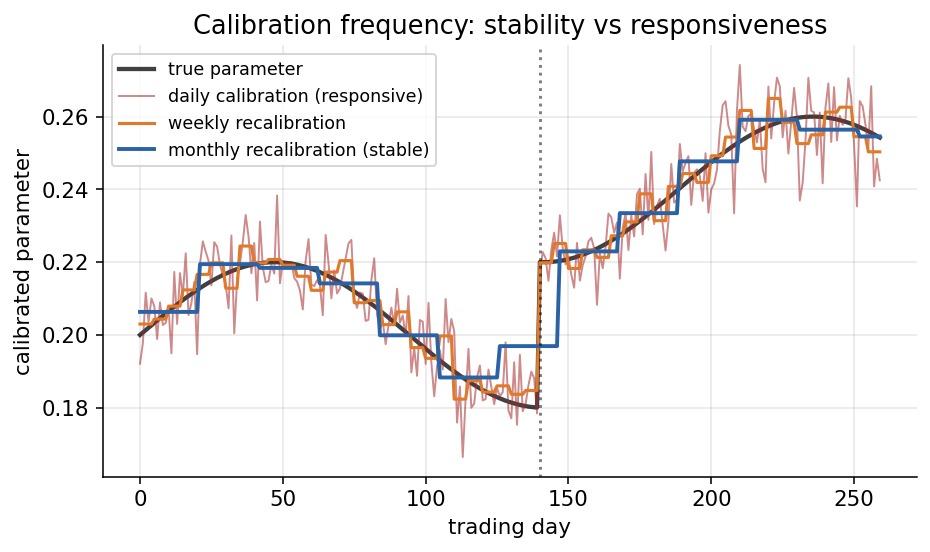
\includegraphics[keepaspectratio]{figures/ch11-frequency-tradeoff.png}}
\emph{A synthetic parameter that drifts smoothly through a regime break
at day 140. \textbf{Daily} recalibration (faint red) is responsive but
noisy; \textbf{monthly} recalibration (blue) is stable but lags the
regime shift by up to a month; \textbf{weekly} recalibration (orange)
sits in between. No frequency dominates --- the trade-off is real and
the choice belongs to the desk's risk-appetite statement.}

\subsection{A.5 The Limits of Market
Consistency}\label{a.5-the-limits-of-market-consistency}

We have emphasised market consistency throughout this chapter, but it
has limits. A market-consistent model reproduces observed prices by
construction. It does \emph{not} predict future prices; it cannot
anticipate regime shifts; it cannot distinguish an informed quote from a
stale one; and it cannot correct for market mispricings that your
analysis has identified.

A value-oriented investor or discretionary trader who has an independent
view about what prices \emph{should be} will deliberately diverge from
market-consistency. They will use models calibrated to \emph{their} view
of fair value, not to the market's quoted mid. This is a different
modelling paradigm, and it is appropriate for certain seats (prop
trading, asset management, hedge funds) but not others (market making,
flow derivatives). For the market maker, consistency with the market is
a must; for the prop trader, the whole point is to be inconsistent with
the market in defensible directions. Calibration, in the
market-consistent sense we have been developing, is therefore a
\emph{specific} modelling discipline associated with \emph{specific}
business functions.

\subsection{A.6 Connections to Machine
Learning}\label{a.6-connections-to-machine-learning}

In recent years, there has been growing interest in using
machine-learning techniques for calibration. The motivation: neural
networks can learn the model pricing function (the map from parameters
to prices) once, and then calibration reduces to inverting this learned
function --- which can be orders of magnitude faster than re-solving the
pricing problem at every optimiser step. A typical setup: generate a
large training dataset of (parameters, prices) pairs by running the
model forward on randomly sampled parameters, train a neural network to
approximate the pricing function, and at calibration time solve an
inverse problem over the network using gradient-based methods that
backpropagate through it. This approach has been applied successfully to
Heston calibration (Chapter 10), Bermudan options, and rough-vol models.
The downsides: the network has to be retrained when the model
specification changes; accuracy in extreme parameter regions is limited
by training-set coverage; and the system inherits the stability issues
of neural networks including adversarial sensitivity and
out-of-distribution failures. For stable well-studied models, the
learning-accelerated calibration is often worth the complexity; for
experimental or custom models, a traditional iterative calibration is
often simpler.

\subsection{A.7 Benchmarking Calibration
Performance}\label{a.7-benchmarking-calibration-performance}

How do you know your calibration is doing a good job? Several benchmarks
are worth tracking on a daily basis. \emph{In-sample fit quality} ---
the average residual across calibration instruments --- should be
comparable to the bid-ask spread, not dramatically smaller (a sign of
overfitting) or larger (a sign of model misspecification).
\emph{Out-of-sample fit quality} on instruments not in the calibration
basket should be comparable to in-sample fit; a large gap indicates
overfitting. \emph{Temporal stability} --- the day-over-day change in
calibrated parameters on a calm day --- should be small; large daily
jumps suggest either an unstable calibration or a genuine market move,
and careful attribution is needed to distinguish them. \emph{Consistency
across product lines}: if the same parameters price multiple products,
residuals on each product's validation instruments should be comparable.
\emph{Predictive power}: for models used in forward-looking analysis,
does the simulated distribution of future prices match what actually
happens? A mature calibration function tracks all of these metrics on
dashboards, alerts on unusual patterns, and escalates to human review
when any threshold is breached.

\subsection{A.8 Calibration Governance and Model
Risk}\label{a.8-calibration-governance-and-model-risk}

Calibration is a regulated activity. Post-2008, banks are required to
maintain formal model-risk-management frameworks that cover calibration
procedures. The typical requirements include documentation of the
calibration methodology (choice of instruments, weighting schemes,
regularisation, numerical methods), independent validation of
statistical properties and out-of-sample performance, monitoring of
calibration outputs over time with alerts for unusual residuals or
parameter jumps, override tracking of any manual adjustments with
documented rationale, and periodic review of the methodology to ensure
it remains fit for purpose under changing market conditions. These
requirements are not bureaucratic overhead; they are defenses against
the failure modes we have discussed throughout the chapter. A
well-calibrated model that no one monitors will silently drift into a
bad regime; a well-monitored model with bad calibration methodology will
produce a documented trail of bad answers. Good governance combines
technical quality with organisational discipline.

\subsection{A.9 A Final Pragmatic
Perspective}\label{a.9-a-final-pragmatic-perspective}

Calibration sits at the intersection of mathematics, statistics,
software engineering, and institutional judgement. It is a deeply
practical discipline, yet it rests on theoretical foundations (FTAP,
change of measure, affine models) as elegant as any in quantitative
finance. The practitioner who masters calibration is mastering the
translation layer between the market's abstract signal and the model's
concrete prediction --- a translation performed dozens of times a day,
across every desk and every product, at every institution that trades
derivatives. Calibration is an inverse problem; it is often ill-posed in
subtle ways; and the three classical pathologies (non-existence,
non-uniqueness, instability) each call for distinct remedies. Moment
matching is the cleanest tool for lattice calibration;
change-of-numeraire machinery is a practical tool, not an abstract
indulgence; and identifiability is never guaranteed. Bid-ask spreads set
a precision floor. With these tools and mindsets in place, calibration
becomes not a mysterious black art but a disciplined craft --- one where
mathematics, code, and judgement combine to extract useful signal from a
noisy, over-determined market, in a way that is auditable, reproducible,
and defensible.

\newpage

\chapter{Chapter 12 --- Short-Rate Models: Vasicek, Ho-Lee, Hull-White,
Affine}\label{chapter-12-short-rate-models-vasicek-ho-lee-hull-white-affine}

\emph{Part IV --- Interest-Rate Models. Depends on Chapter 3 (Itô, OU
solution), Chapter 4 (Feynman-Kac for bond pricing), Chapter 5 (Girsanov
for the passage from the physical measure \(\mathbb{P}\) to the
risk-neutral measure \(\mathbb{Q}\)), and Chapter 11 (calibration on
lattices).}

This is the chapter in which the yield curve becomes an object we can
\emph{model} rather than merely observe. The calibration chapter
(Chapter 11) built short-rate lattices by matching observed bond prices
term by term; here we replace the lattice with a continuous-time
stochastic differential equation and derive closed-form bond prices,
yield curves, and volatility structures from the dynamics themselves.
Three models --- Vasicek, Ho-Lee, and Hull-White --- are developed as a
single narrative, with Vasicek as the canonical derivation that the
other two specialise or extend. The applications (interest-rate swaps,
CDS, bond options, callable bonds) live in Chapter 13; the caps, floors,
and swaptions capstone lives in Chapter 14. This chapter's single job is
to build the model.

\section{12.1 Motivation and the traded
primitives}\label{motivation-and-the-traded-primitives}

In equity pricing the underlying \(S_t\) is itself the traded asset, so
no-arbitrage directly pins its \(\mathbb{Q}\)-drift at \(r\). In rates
the state variable \(r_t\) and the tradables are \emph{different}: the
short rate itself cannot be bought, so the Fundamental Theorem of Asset
Pricing pins down \(\mathbb{Q}\) only through its action on what
\emph{is} traded. This is the conceptual pivot of the chapter, and it is
what makes a ``calibration'' step necessary for rates models in a way
that it isn't for equities.

The traded primitives are:

\begin{itemize}
\tightlist
\item
  the money-market (bank) account
\end{itemize}

\[
\mathrm{d}M_t = r_t\, M_t\, \mathrm{d}t, \qquad M_0 = 1,
\tag{12.1}
\]

equivalently \(M_t = \exp\!\big(\int_0^t r_s\, \mathrm{d}s\big)\); -
zero-coupon bonds of various maturities \(T\), with price process
\(\big(P_t(T)\big)_{0\le t\le T}\) and terminal condition
\(P_T(T) = 1\). Bonds are contingent claims on the \emph{path} of
\(r_s\) --- every bond pays \$1 at maturity, so its value today is
determined by the law of \(\int_0^T r_s\,\mathrm{d}s\).

The ambition of the short-rate programme is dramatic compression: posit
a single scalar SDE for \(r_t\), and from that one equation recover the
entire yield curve plus consistent prices for every rate-sensitive
derivative written on it. The compression succeeds because the required
structural ingredients (linear drift, linear-or- state-dependent squared
volatility, Markovian state) are exactly the conditions for the
affine-pricing apparatus to work. A non-affine short-rate model would
fail to produce tractable bond prices, and would therefore fail to
support the edifice of rate-derivative pricing. Affine structure is both
the secret of the model's success and the source of its limitations.

Short-rate models are \emph{not} forecasting tools. A Vasicek model fed
today's yield curve and today's implied vols says nothing useful about
whether rates will rise or fall under \(\mathbb{P}\); it says only what
price today's arbitrage conditions impose on a derivative, given the
\(\mathbb{Q}\)-dynamics. The term premium --- the gap between
\(\mathbb{Q}\) and \(\mathbb{P}\) expectations of future rates --- is a
free input to the model, not an output. Macroeconomics, surveys, or
factor models answer ``where will rates go?''; Vasicek and its cousins
answer ``what is the arbitrage-free swaption price given the dynamics?''
Confusing the two is the most common conceptual mistake in rates
modelling.

\subsection{\texorpdfstring{12.1.1 Non-uniqueness of \(\mathbb{Q}\) on a
rate
tree}{12.1.1 Non-uniqueness of \textbackslash mathbb\{Q\} on a rate tree}}\label{non-uniqueness-of-mathbbq-on-a-rate-tree}

On an equity tree the risk-neutral probability \(q\) is pinned down by
no-arbitrage once \(u, d, r\) are fixed:
\(q = (e^{r\Delta t} - d)/(u - d)\). On a rate tree the corresponding
\(q\) is \emph{not} unique, because the FTAP pins \(\mathbb{Q}\) only
through tradables and the short rate isn't one. Different short-rate
dynamics can reproduce the same observed bond prices, and arbitrage
cannot distinguish between them. Chapter 11 §11.3 made this
discrete-time underdetermination concrete: at every step the tree adds
one observation (a bond quote) and more than one free parameter (rate
nodes plus a transition probability), so the system is perpetually
under-determined and external information (calibration to market bonds)
is needed to pin down the model.

\begin{quote}
\textbf{Slogan.} \emph{The short-rate tree is not the price of a traded
asset, so \(q\) is not uniquely determined by no-arbitrage. The market
bond prices supply the external information that pins down \(\theta\).}
\end{quote}

This is the discrete-time shadow of the continuous-time statement that
Hull-White has infinitely many \(\theta(t)\) choices for any given
\((\kappa, \sigma)\), and only the curve-fit picks one out.

\section{12.2 Discrete motivation: AR(1) and the continuous
limit}\label{discrete-motivation-ar1-and-the-continuous-limit}

Why does an AR(1) belong here at all? Because empirical short-rate
series (Fed funds, EONIA, SONIA, SOFR) look remarkably unlike random
walks and remarkably like stationary mean-reverting processes. Plot a
multi-decade history of a policy rate and it moves in slow waves that
hover around levels broadly set by trend inflation and potential growth;
it does not diffuse toward infinity the way a geometric Brownian motion
would. The simplest model that captures this is a linear combination of
yesterday's rate, a drift toward a mean, and a Gaussian shock --- the
discrete AR(1):

\[
r_n \;=\; \alpha\, r_{n-1} \;+\; \beta_n \;+\; \sigma\sqrt{\Delta t}\, \varepsilon_n,
\qquad \varepsilon_n \stackrel{\text{iid}}{\sim} \mathcal{N}(0,1).
\tag{12.2}
\]

Rewriting (12.2) in ``innovation form,''

\[
r_n - r_{n-1} \;=\; \kappa(\theta - r_{n-1})\,\Delta t \;+\; \sigma\sqrt{\Delta t}\,\varepsilon_n,
\tag{12.3}
\]

makes the correspondence with a continuous mean-reverting SDE
transparent. Identifying \(\alpha \leftrightarrow 1 - \kappa\Delta t\),
\(\beta_n \leftrightarrow \kappa\theta\Delta t\), and
\(\varepsilon_n\sqrt{\Delta t} \leftrightarrow \mathrm{d}W_t\), and
sending \(\Delta t \to 0\), recovers the Vasicek SDE

\[
\mathrm{d}r_t \;=\; \kappa(\theta - r_t)\,\mathrm{d}t \;+\; \sigma\,\mathrm{d}W_t.
\tag{12.4}
\]

The persistence \(\alpha\) and the mean-reversion speed \(\kappa\) are
two views of the same quantity: \(\alpha = e^{-\kappa\Delta t}\) in
exact correspondence, and for small \(\Delta t\) this is well
approximated by \(1 - \kappa\Delta t\). A daily AR(1) with
\(\alpha = 0.998\) corresponds to
\(\kappa = -\ln(0.998)/(1/252) \approx 0.50\) --- a roughly-annual
mean-reversion speed consistent with empirical policy rates.

The other useful intuition from the AR(1) view is that the
continuous-time process \(r_t\) has \emph{memory}. Under geometric
Brownian motion (the Black-Scholes stock model) today's price contains
no information about tomorrow's trajectory beyond its own level; under
Vasicek, today's rate contains information about the \emph{deviation
from the mean} that partially persists. This memory is what makes mean
reversion predictable at longer horizons --- not because we can forecast
the noise, but because we know the drift will systematically pull the
process back toward \(\theta\) at an estimable rate. For derivatives
pricing this matters: an option that pays off a function of the
integrated rate over time is fundamentally a bet on these mean-reverting
dynamics, and its price depends sensitively on how much memory the
process has.

\subsection{12.2.1 Why continuous time?}\label{why-continuous-time}

The continuous limit is not just aesthetic. In discrete time, pricing a
\(T\)-year zero-coupon bond means computing an expectation of a product
of \(T/\Delta t\) correlated random discount factors --- a
high-dimensional integral with no closed form. In continuous time, by
contrast, the same object becomes an expectation of the exponential of a
Gaussian integral, whose moment-generating function is explicit.
Continuous time is what unlocks the closed-form bond price
\(P_t(T) = e^{A_t(T) - B_t(T)r_t}\) that makes the calibration and
hedging machinery workable.

The gap between a continuous-time Vasicek and a sensible daily discrete
approximation is, in practice, negligible compared with
model-specification error, parameter-estimation error, or liquidity
effects. Nobody should lose sleep over the ``continuous vs discrete''
dichotomy once calibration is done. What matters is that continuous time
gives us a tractable language in which to express and solve pricing
problems; the language is a tool, not a claim about ontology.

There is also a pedagogical virtue to continuous time. In discrete time,
the various random-walk and AR(1) models look superficially similar ---
they differ only in the fine print of their coefficients --- and it is
easy to lose sight of which model is adequate for a given problem. In
continuous time the functional forms of drifts and diffusions are
starker and more revealing: a constant drift is obviously different from
a linear-in-state drift, a constant diffusion is obviously different
from a \(\sqrt{r}\) diffusion. The continuous-time formulation makes the
modelling choices \emph{legible}, and legibility is a precondition for
careful thinking.

\subsection{12.2.1.b Estimating AR(1) Vasicek from historical
data}\label{b-estimating-ar1-vasicek-from-historical-data}

The AR(1) representation (12.3) is useful not only pedagogically but for
parameter estimation. Given a time series of observations
\(\{r_0, r_1, \ldots, r_N\}\) on a \(\Delta t\) grid, ordinary least
squares regression of \(r_n\) on \(r_{n-1}\) yields estimates of the
slope \(\beta =
1 - \kappa\Delta t\) and intercept \(\kappa\theta\Delta t\), from which
\(\kappa = (1 - \beta)/\Delta t\) and \(\theta = \alpha/(1 - \beta)\)
follow directly. The residuals from this regression have variance
\(\sigma^2
\Delta t\), giving an estimate of \(\sigma\). This simple estimation
procedure is the physical-measure (\(\mathbb{P}\)) calibration of
Vasicek, and it can be implemented in a few lines of linear algebra ---
a reminder that many ``exotic'' quantitative finance tools reduce to
well-known statistical procedures once the algebra is peeled away.

The sample autocorrelation at lag \(h\) ---
\(\text{Corr}(r_s, r_{s+h})\) --- should follow the theoretical form
\(e^{-\kappa h}\) in stationary equilibrium. Plotting empirical
autocorrelation against lag on a log-linear scale and fitting a straight
line is a quick diagnostic of whether the data are well-described by an
OU / AR(1) process. If the empirical autocorrelation decays
exponentially, the AR(1) is a good fit; if it decays faster
(over-damped) or slower (long memory), the data are telling you
something the simple model misses. Long memory is a particularly
well-studied deviation; models with multiple mean-reversion speeds
(G2++, three-factor affine) capture it by having one slow and one fast
factor.

Two important identifiability warnings. First, estimates of \(\kappa\)
are notoriously noisy in short samples: the ``half-life of a shock'' is
a slow-moving feature, and short-window data contains limited
information about it. Robust estimates typically require decades of
daily data, or at least years of high-frequency data. Second, the
physical-measure estimates of \(\kappa^{\mathbb{P}}\) and
\(\theta^{\mathbb{P}}\) differ systematically from their risk-neutral
counterparts \(\kappa^{\mathbb{Q}}\) and \(\theta^{\mathbb{Q}}\) by the
market price of risk. The volatility \(\sigma\) is measure-invariant
(Girsanov changes drift but not diffusion), so it should theoretically
agree across historical and calibration estimates --- a useful sanity
check when running both.

\subsection{\texorpdfstring{12.2.2 From \(\mathbb{P}\) to \(\mathbb{Q}\)
(cross-reference Chapter
5)}{12.2.2 From \textbackslash mathbb\{P\} to \textbackslash mathbb\{Q\} (cross-reference Chapter 5)}}\label{from-mathbbp-to-mathbbq-cross-reference-chapter-5}

Under the physical measure \(\mathbb{P}\), write the short rate as

\[
\mathrm{d}r_t \;=\; \mu(t,r_t)\,\mathrm{d}t \;+\; \sigma(t,r_t)\,\mathrm{d}W_t.
\tag{12.5}
\]

By Girsanov's theorem (Chapter 5), the change of measure to the
risk-neutral \(\mathbb{Q}\) shifts the drift by
\(-\lambda_t\,\sigma(t, r_t)\), where \(\lambda_t\) is the \emph{market
price of interest-rate risk}:

\[
\mathrm{d}r_t \;=\; \big(\mu(t, r_t) - \lambda_t\,\sigma(t, r_t)\big)\,\mathrm{d}t \;+\; \sigma(t, r_t)\,\mathrm{d}\widehat{W}_t.
\tag{12.6}
\]

We do not re-derive Girsanov here --- that happened in Chapter 5, where
the density process, Doléans-Dade exponential, and two-numeraire
switching were developed as the canonical treatment. What matters for
this chapter is the consequence. Three standard choices of \(\lambda_t\)
preserve the affine structure:

\begin{itemize}
\tightlist
\item
  Constant \$\lambda\_t = \$ const: only shifts \(\theta\) (the long-run
  mean under \(\mathbb{Q}\) differs from that under \(\mathbb{P}\)).
\item
  Affine in \(r_t\): \(\lambda_t = a + b\,r_t\): shifts both \(\theta\)
  and \(\kappa\).
\item
  Deterministic function of time \(\lambda_t = a_t + b_t\,r_t\): yields
  Hull-White with time-dependent \(\theta_t\).
\end{itemize}

All three preserve the linear drift, and under \(\mathbb{Q}\) the short
rate continues to satisfy

\[
\mathrm{d}r_t \;=\; \kappa(\theta_t - r_t)\,\mathrm{d}t \;+\; \sigma\,\mathrm{d}\widehat{W}_t,
\tag{12.7}
\]

where \(\theta_t\) is (in general) a deterministic function of time. The
diffusion \(\sigma\) does \emph{not} change under Girsanov: Brownian
motions have the same quadratic variation under equivalent measures, so
calibrated volatilities carry over directly across measure
specifications without needing adjustment. Only drifts change when
measures change.

The economic content of \(\lambda_t\) is worth a pause. Under
\(\mathbb{P}\) rate shocks are perceived as risky, and investors demand
compensation for holding bonds whose prices move inversely to those
shocks. That compensation is the term premium, and it biases the
\(\mathbb{P}\)-drift of \(r_t\) relative to what a risk-neutral agent
would perceive. Because we never directly observe \(\lambda_t\) --- we
only see prices, and prices aggregate \(\mathbb{P}\)-dynamics with
\(\lambda_t\) into a single \(\mathbb{Q}\)-drift --- the modelling
convention is to work entirely under \(\mathbb{Q}\) and let historical
data inform the shape (if any) of \(\lambda_t\) separately. In
short-rate modelling for pricing, it is almost universal to specify
dynamics directly under \(\mathbb{Q}\) and never write
\(\mathbb{P}\)-dynamics explicitly.

\subsection{12.2.3 The fundamental bond-pricing
formula}\label{the-fundamental-bond-pricing-formula}

By the general theory of risk-neutral pricing (Chapter 5), relative
prices of all traded assets are \(\mathbb{Q}\)-martingales once we
divide by the numeraire \(M_t\). For a zero-coupon bond with terminal
payoff 1,

\[
\frac{P_t(T)}{M_t} \;=\; \mathbb{E}^{\mathbb{Q}}_t\!\left[\,\frac{1}{M_T}\,\right]
\qquad\Longrightarrow\qquad
\boxed{\;\; P_t(T) \;=\; \mathbb{E}^{\mathbb{Q}}_t\!\left[\, e^{-\int_t^T r_s\,\mathrm{d}s}\,\right]. \;\;}
\tag{12.8}
\]

Equation (12.8) is the master formula of short-rate modelling. Read
carefully, it says that today's bond price is \emph{exactly} the
risk-neutral expectation of the continuously-compounded discount factor
over the bond's life. This sentence contains a lot: it simultaneously
asserts no-arbitrage (the price is an expectation), identifies the right
measure (\(\mathbb{Q}\)), specifies the right numeraire (\(M_t\)), and
provides a concrete algorithm (integrate \(r_s\) along simulated paths
and average). Every bond price in this chapter --- and every yield,
forward rate, swap rate, caplet, and swaption derived from bond prices
in Chapter 13 --- is a consequence of this formula.

A useful consistency check: when \(r_t = r\) is deterministic and
constant, (12.8) reduces to \(P_t(T) = e^{-r(T-t)}\). When \(r_t\) is
deterministic but time-varying, it reduces to \(P_t(T) = e^{-\int_t^T
r_s\,\mathrm{d}s}\). Only when \(r_t\) is stochastic does the
expectation become non-trivial; the formula generalises the
deterministic cases smoothly and recovers them as special limits.

The algorithmic reading of (12.8) is equally important. If we cannot
evaluate the expectation analytically --- say, because the model is too
complex for a closed form --- we can always simulate: generate many
Monte Carlo paths of \(r_t\) from \(t\) to \(T\) under \(\mathbb{Q}\),
compute the realised discount factor along each path, and average. The
bond price converges in probability to the average as the number of
paths grows. The entire business of finding closed forms (the affine
trick we are about to execute) is a way of \emph{avoiding} Monte Carlo
by exploiting special structure; when that structure is absent, Monte
Carlo is there to catch us.

\begin{center}\rule{0.5\linewidth}{0.5pt}\end{center}

\section{12.3 Vasicek --- the canonical
derivation}\label{vasicek-the-canonical-derivation}

This is the technical heart of the chapter. Take (12.7) with constant
\(\theta\), which gives the original Vasicek (1977) model:

\[
\boxed{\;\; \mathrm{d}r_t \;=\; \kappa(\theta - r_t)\,\mathrm{d}t \;+\; \sigma\,\mathrm{d}\widehat{W}_t, \qquad \kappa, \theta, \sigma > 0. \;\;}
\tag{12.9}
\]

The drift is linear-restoring, the diffusion is constant, and the
solution is an Ornstein-Uhlenbeck process: a mean-reverting Gaussian
process with long-run mean \(\theta\) and mean-reversion speed
\(\kappa\).

\textbf{Intuition --- mean reversion.} Whenever \(r_t\) wanders above
\(\theta\), the drift pulls it \emph{down} in proportion to the
deviation; when it drifts below, the drift pushes it \emph{up}.
Economically this mirrors the behaviour of real short rates --- central
banks tighten when rates are ``too low'' (inflation pressure) and ease
when they are ``too high'' (recession risk), so rates orbit around a
neutral level rather than random-walking. The speed \(\kappa\) controls
how fast this happens: the \emph{half-life} of deviations is
\(\ln 2/\kappa\). With \(\kappa = 0.3\) a shock decays by half in about
2.3 years; with \(\kappa = 1.0\), in about 8 months. The stationary
distribution is \(\mathcal{N}(\theta, \sigma^2/(2\kappa))\) --- larger
\(\kappa\) (stronger pull) or smaller \(\sigma\) (less noise) narrows
the long-run distribution around \(\theta\).

The half-life interpretation deserves emphasis because it is how
practitioners think about \(\kappa\). Nobody calibrating reasons
directly in units of ``inverse time'' --- they reason in half-lives,
because a half-life has immediately physical meaning. ``A \(\kappa\) of
0.3 corresponds to a rate-shock half-life of 2.3 years'' is a statement
any rates trader can sanity-check against intuition about how long a
Fed-funds deviation persists before the next cutting or hiking cycle
unwinds it. If a calibrated \(\kappa\) implies a half-life that is
wildly too short (weeks) or absurdly too long (decades), something is
wrong.

The Gaussian structure is the other defining feature of Vasicek. It is
what makes every subsequent computation tractable: a linear combination
of Gaussian increments is Gaussian, an integral of Gaussians is
Gaussian, and the exponential of a Gaussian has a closed-form mean (its
moment-generating function). The whole affine bond-price formula
ultimately rests on this one fact. The price paid is that \(r_t\) can,
in principle, go negative: the Gaussian distribution is supported on all
of \(\mathbb{R}\). Before the 2008-2020 era of unconventional monetary
policy, this was viewed as the model's most conspicuous defect. After
2014 several European and Japanese policy rates did go meaningfully
negative, and suddenly Vasicek's ability to accommodate negative rates
became a \emph{feature}, not a bug. No other equally tractable
short-rate model handles negative rates so naturally.

\begin{figure}
\centering
\pandocbounded{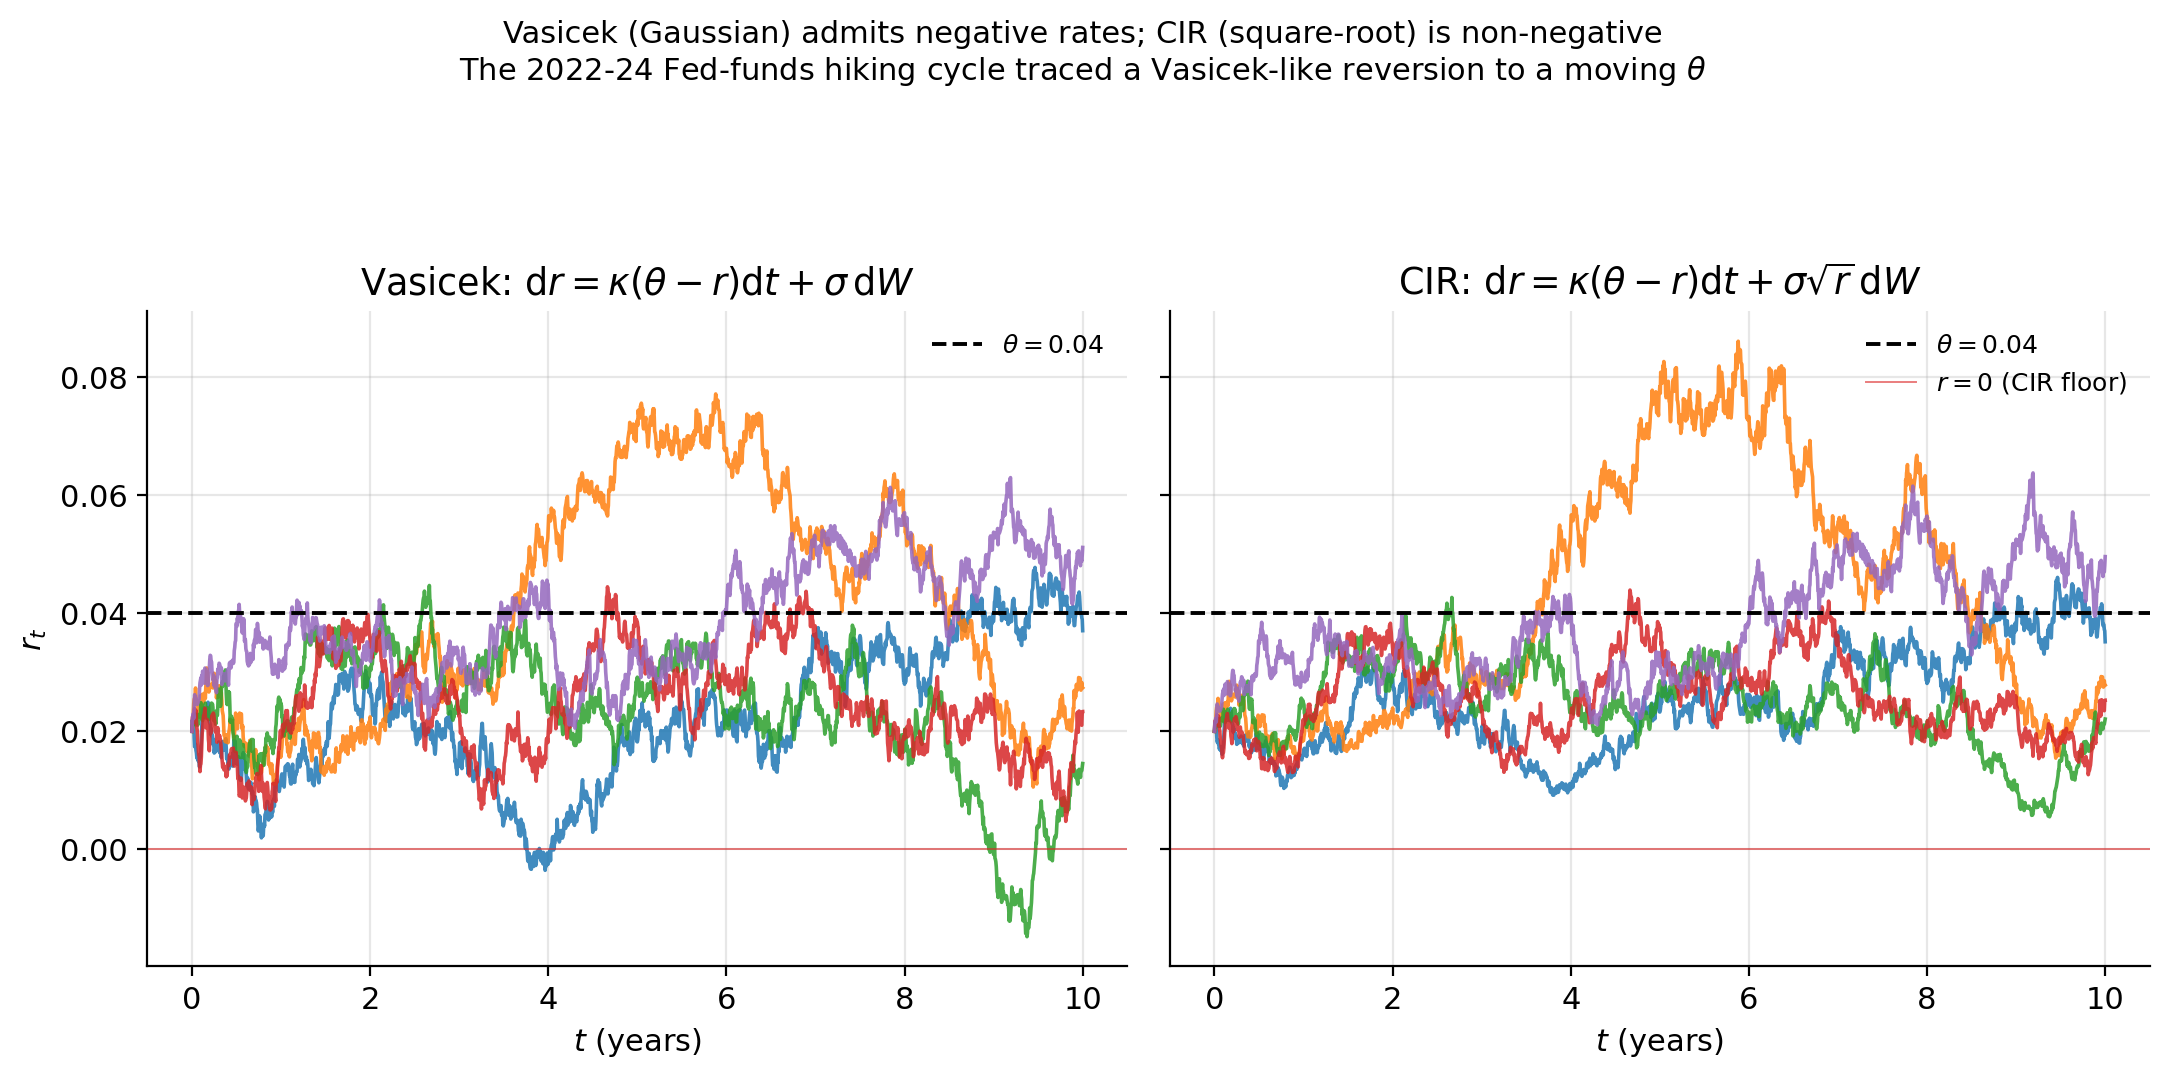
\includegraphics[keepaspectratio]{figures/ch12-vasicek-vs-cir.png}}
\caption{Vasicek (Gaussian, can go negative) versus CIR (square-root
diffusion, non-negative) sample paths under matched \(\kappa\),
\(\theta\). The 2014-2022 ECB deposit rate stayed below zero --- a
regime where Vasicek fit cleanly and CIR could not}
\end{figure}

\subsection{12.3.1 The SDE and the explicit
solution}\label{the-sde-and-the-explicit-solution}

Solve (12.9) by the standard OU integrating factor. Set
\(r_t = e^{-\kappa t} g_t\) (equivalently \(g_t = e^{\kappa t} r_t\)).
By Itô's lemma (Chapter 3),

\[
\mathrm{d}r_t = -\kappa\, e^{-\kappa t} g_t\,\mathrm{d}t \;+\; e^{-\kappa t}\,\mathrm{d}g_t = -\kappa r_t\,\mathrm{d}t + e^{-\kappa t}\,\mathrm{d}g_t.
\tag{12.10}
\]

Matching (12.10) against (12.9),

\[
\mathrm{d}g_t \;=\; \kappa\, e^{\kappa t}\,\theta\,\mathrm{d}t \;+\; \sigma\, e^{\kappa t}\,\mathrm{d}\widehat{W}_t.
\tag{12.11}
\]

Integrate from \(t\) to \(T\) and rearrange using
\(g_T - g_t = e^{\kappa T}r_T - e^{\kappa t}r_t\):

\[
\boxed{\;\; r_T \;=\; e^{-\kappa(T-t)}\, r_t \;+\; \theta\!\left(1 - e^{-\kappa(T-t)}\right) \;+\; \sigma\!\int_t^T e^{-\kappa(T-s)}\,\mathrm{d}\widehat{W}_s. \;\;}
\tag{12.12}
\]

The integrating-factor trick used here generalises to essentially every
linear SDE. The key move is multiplying through by \(e^{\kappa t}\),
which converts the mean-reverting term \(-\kappa r_t\,\mathrm{d}t\) into
a pure differential. Once that is done, the remaining drift and
diffusion have no \(r_t\) dependence and can be integrated directly ---
the non-trivial feedback has been algebraically removed. The price of
admission is that the final expression involves a weighted stochastic
integral against the kernel \(e^{-\kappa(T-s)}\), with weights that
decay exponentially as you look further back. These decaying weights
have a beautiful physical meaning: the current short rate is a weighted
average of all past shocks, with older shocks discounted more heavily
because the mean-reverting drift has had more time to ``forget'' them.
This is exactly the continuous-time analogue of a discrete AR(1) with
autoregressive coefficient \(e^{-\kappa\Delta t}\).

The structural similarity between (12.12) and the Ornstein-Uhlenbeck
result in physics is worth noting: there an OU process describes the
velocity of a particle undergoing Brownian motion in a viscous fluid.
The mean-reverting drift \(\kappa(\theta - r_t)\) is analogous to a
frictional force pulling the velocity toward equilibrium; the diffusion
\(\sigma\,\mathrm{d}\widehat{W}_t\) is analogous to random molecular
collisions. The exponential memory of past shocks is the mathematical
signature of frictional damping. All classical physical intuition about
coloured noise, spectral densities, and correlation times carries
directly across to interest-rate modelling.

Read (12.12) piece by piece: the first term \(e^{-\kappa(T-t)}r_t\) is
the \emph{deterministic} decay of the current rate toward the mean; the
second term \(\theta(1 - e^{-\kappa(T-t)})\) is the deterministic
buildup of the mean-reversion level; the third term is a mean-zero
Gaussian random variable whose variance grows from 0 (at \(T=t\)) toward
the stationary value \(\sigma^2/(2\kappa)\) (as \(T\to\infty\)). Three
effects neatly separated: where we are now, how fast we revert, how
noisy the journey is. Every intuition about OU processes --- and
therefore about Vasicek, Hull-White, and half the short-rate literature
--- can be read off this one equation.

\subsection{12.3.1.b Joint distribution over multiple
times}\label{b-joint-distribution-over-multiple-times}

A property of (12.12) that matters in practice: the joint distribution
of \((r_{t_1}, r_{t_2}, \ldots, r_{t_n})\) at any finite collection of
times is multivariate Gaussian. This follows because each \(r_{t_i}\) is
an affine function of the same Brownian motion, and linear combinations
of a Brownian path are jointly Gaussian. The mean and covariance of this
multivariate Gaussian can be computed explicitly:

\[
\mathrm{Cov}(r_s, r_t) \;=\; \sigma^2\,e^{-\kappa(s+t)}\!\int_0^{\min(s,t)} e^{2\kappa u}\,\mathrm{d}u \;=\; \frac{\sigma^2}{2\kappa}\!\left(e^{-\kappa|t-s|} - e^{-\kappa(t+s)}\right).
\tag{12.12a}
\]

The dominant term is the exponentially decaying autocorrelation
\(e^{-\kappa|t-s|}\); the subtracted term accounts for the boundary
effect near \(t = s = 0\). In the stationary limit
(\(s, t \gg 1/\kappa\)) the covariance reduces to
\(\frac{\sigma^2}{2\kappa} e^{-\kappa|t-s|}\), exactly matching the
classical OU correlation structure.

This multivariate-Gaussian structure is what makes \emph{exact} Monte
Carlo simulation of Vasicek paths so efficient. If you need samples at
specific times \(\{t_1, \ldots, t_n\}\), you can compute the exact
covariance matrix, Cholesky-factor it, and draw correlated Gaussians in
one shot --- no Euler discretisation error. For Monte Carlo of payoffs
that depend only on terminal rates (e.g.~European bond options) you do
not even need the full covariance matrix; a single Gaussian draw for
\(r_T\) suffices. CIR, by contrast, does not admit this luxury: its
non-central chi-squared distribution is exact but more awkward to
sample. The analytical tractability of Vasicek therefore extends beyond
pricing into simulation efficiency --- a reason to prefer Vasicek when
it fits.

\subsection{\texorpdfstring{12.3.2 Distribution of
\(r_T\)}{12.3.2 Distribution of r\_T}}\label{distribution-of-r_t}

From (12.12), \(r_T\) conditional on \(\mathcal{F}_t\) is Gaussian with

\[
\mathbb{E}^{\mathbb{Q}}_t[r_T] \;=\; e^{-\kappa(T-t)}\,r_t + \theta\bigl(1 - e^{-\kappa(T-t)}\bigr),
\tag{12.13}
\]

\[
\mathbb{V}^{\mathbb{Q}}_t[r_T] \;=\; \sigma^2\!\int_t^T e^{-2\kappa(T-s)}\,\mathrm{d}s \;=\; \frac{\sigma^2}{2\kappa}\!\left(1 - e^{-2\kappa(T-t)}\right).
\tag{12.14}
\]

The variance starts at 0 at \(T = t\) (no time, no uncertainty) and
saturates at \(\sigma^2/(2\kappa)\) as \(T \to \infty\) (the stationary
variance). The half-saturation time is \(\ln 2/(2\kappa)\), so half of
the stationary variance accumulates in \(\ln 2/(2\kappa)\) years. With
\(\kappa = 0.3\) this is about 1.15 years --- meaning over a 1-year
horizon, rates have accumulated about half their long-run uncertainty.
Beyond about \(5/(2\kappa) \approx 8\) years the distribution is
essentially stationary.

A worked example sharpens this. Take \(\kappa = 0.3\) (half-life about
2.3 years) and \(\sigma = 0.01\) (annualised 100 bp vol). The stationary
standard deviation is \(\sigma/\sqrt{2\kappa} = 0.01/\sqrt{0.6} \approx
0.0129\), or 129 basis points. A normal distribution with this standard
deviation would put roughly two-thirds of its mass within \(\theta \pm
129\) bp and 95\% within \(\theta \pm 258\) bp. For \(\theta = 0.04\)
that gives a plausible long-run range of roughly \(1\%\) to \(7\%\) for
the short rate --- consistent with the long-run range of actual policy
rates in mature economies. Had we taken \(\sigma = 0.03\) (a highly
volatile regime), the stationary sd would be 387 bp and the 95\% band
would extend from \(-3.7\%\) to \(+11.7\%\), clearly including negative
rates. This explicit scaling is one of Vasicek's virtues: it lets you
read off the implications of parameter choices in two-second mental
math.

The ratio \((1 - e^{-2\kappa(T-t)})\) is a useful ``mixing fraction''
that tells you how close to stationarity the process is at horizon
\(T - t\). At \(T - t = 1/\kappa\) (one mean-reversion time) the mixing
fraction is \(1 - e^{-2} \approx 0.865\). At \(T - t = 2/\kappa\) it is
about 0.982. For practical purposes one can treat any horizon beyond
\(3/\kappa\) as effectively stationary, and this is how simulation
studies typically validate their ``burn-in'' periods before extracting
stationary statistics.

\pandocbounded{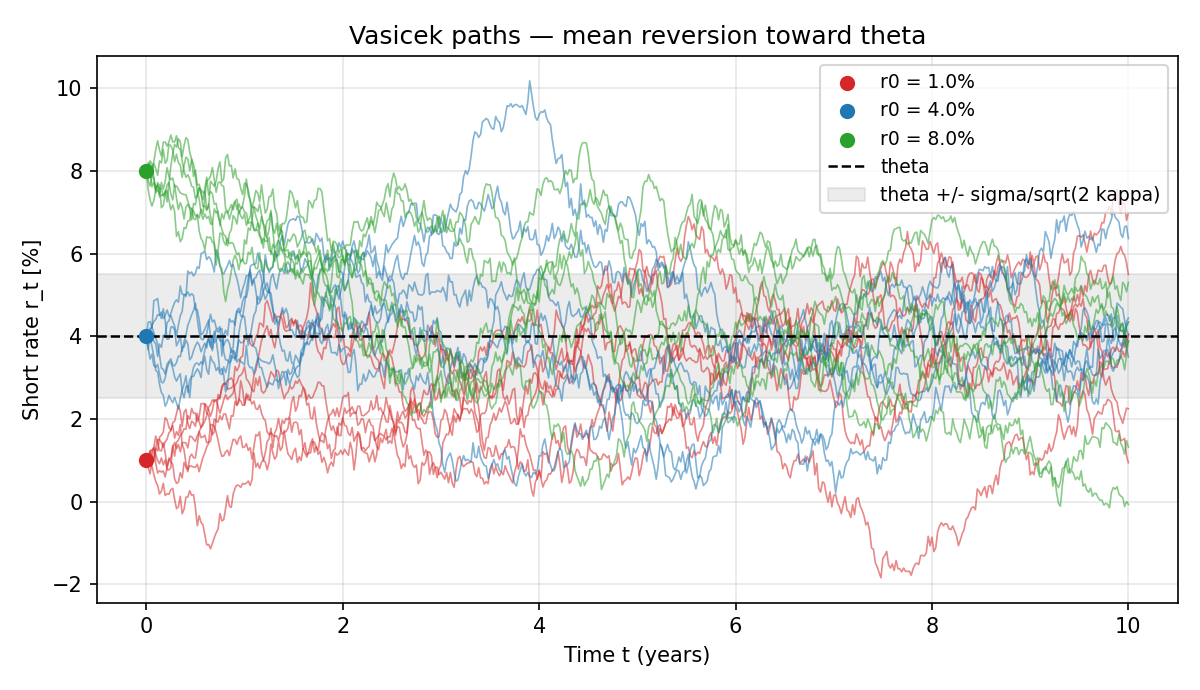
\includegraphics[keepaspectratio]{figures/ch12-vasicek-paths.png}}
\emph{Vasicek paths from three starting points all pull toward
\(\theta\) (dashed line), with dispersion widening then stabilising at
\(\sigma/\sqrt{2\kappa}\).}

\begin{figure}
\centering
\pandocbounded{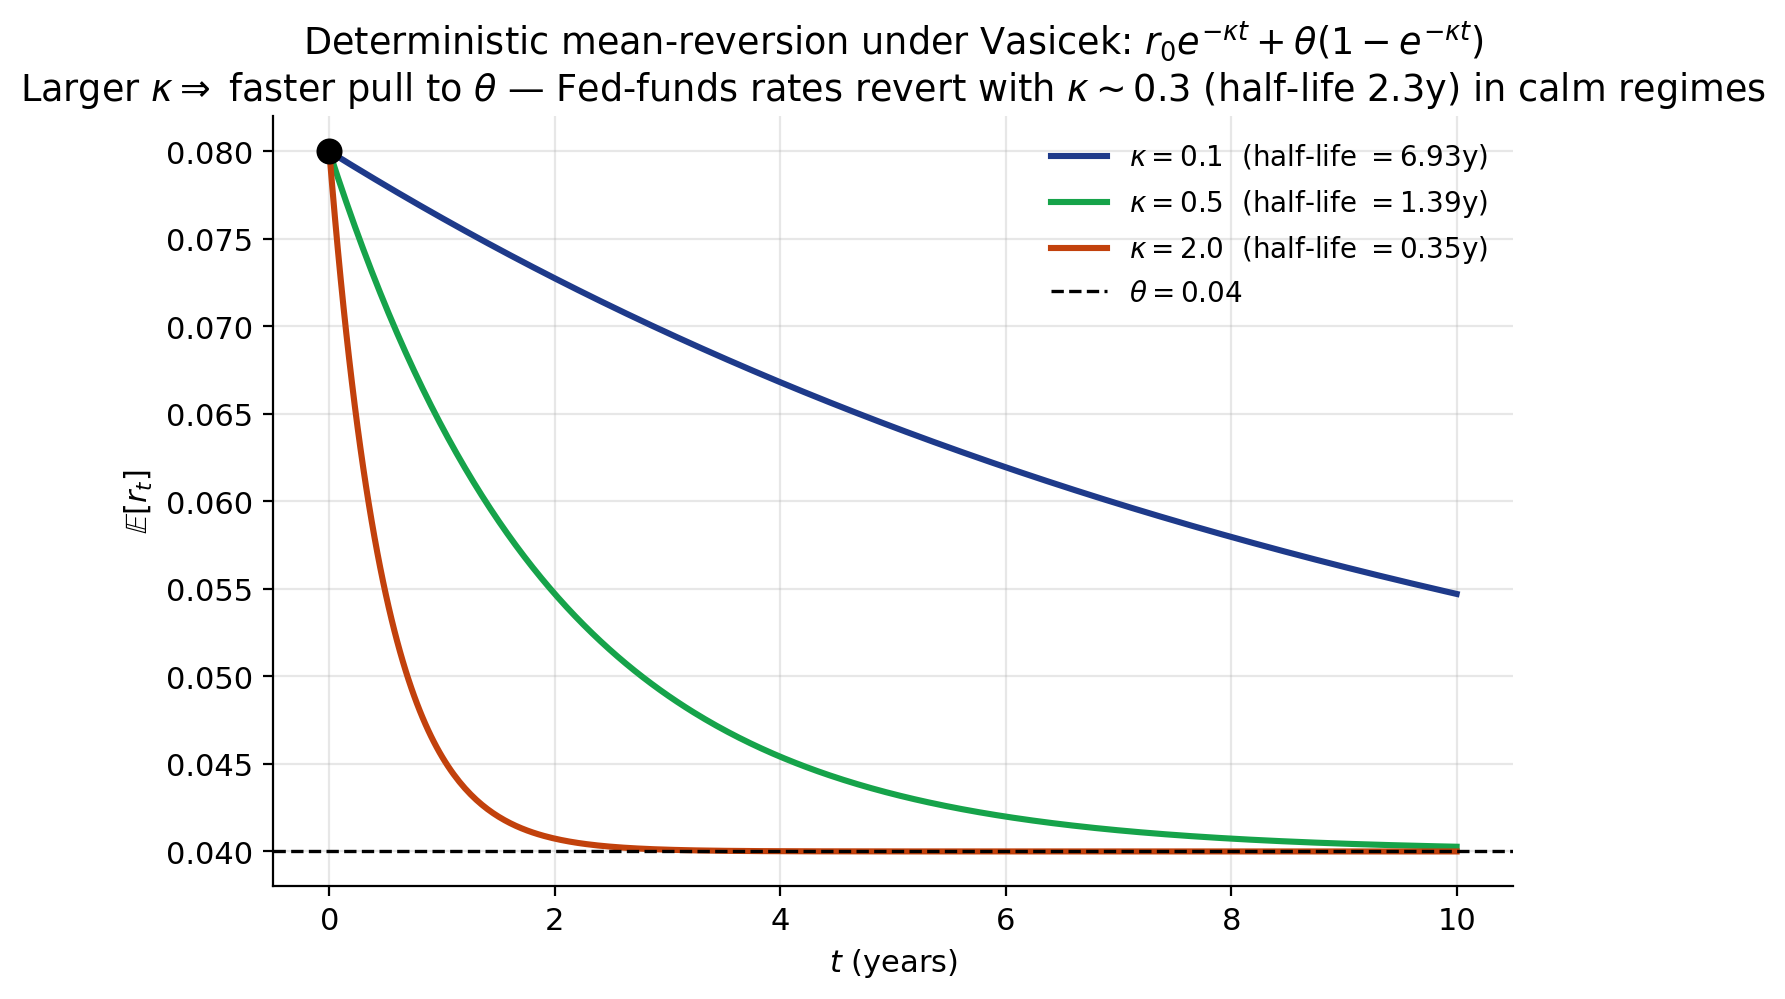
\includegraphics[keepaspectratio]{figures/ch12-mean-reversion-speeds.png}}
\caption{Deterministic mean-reversion under Vasicek for three \(\kappa\)
values: the half-life \(\log 2/\kappa\) controls how fast deviations
from \(\theta\) decay. The Fed-funds rate's reversion toward an evolving
long-run ``neutral'' has empirical \(\kappa \sim 0.3\) --- half-life
about 2.3 years, consistent with typical hiking-cycle horizons}
\end{figure}

There is a visual intuition worth internalising: draw the
\((t, r)\)-plane with a horizontal line at \(r = \theta\). The rate
process starts at \((0, r_0)\). In the deterministic case (set
\(\sigma = 0\)), the path is an exponential curve approaching \(\theta\)
asymptotically:

\[
r_t \;=\; r_0\,e^{-\kappa t} \;+\; \theta\bigl(1 - e^{-\kappa t}\bigr).
\tag{12.13a}
\]

In the stochastic case, this curve is the ``centreline'' around which
sample paths fluctuate, with Gaussian noise amplitude growing from zero
(at \(t = 0\) the rate is deterministically \(r_0\)) toward the
stationary value \(\sqrt{\sigma^2/(2\kappa)}\) as \(t \to \infty\).
Drawing many sample paths overlaid on the same axes produces an
``hourglass'' pattern: tight at \(t = 0\), fanning out over time,
eventually settling into a constant-width band centred at \(\theta\).

Concrete numbers: with \(\kappa = 0.15\), \(\theta = 4\%\),
\(r_0 = 2\%\), the deterministic rate path rises from 2\% toward 4\%
along an exponential with half-life \(\ln 2/0.15 \approx 4.6\) years.
\(\mathbb{E}[r_1] \approx 2.28\%\), \(\mathbb{E}[r_5] \approx 3.06\%\),
\(\mathbb{E}[r_{20}] \approx 3.90\%\). The approach is exponential: the
gap to \(\theta\) halves every 4.6 years. If instead \(r_0 = 6\%\)
(above target), the trajectory is inverted --- an exponential decay from
6\% down toward 4\%, same timescales. In either case the mean rate at
time \(t\) is a specific weighted average of starting point and target,
with weights determined entirely by \(\kappa t\).

\textbf{Intuition for the stationary variance \(\sigma^2/(2\kappa)\).}
Each incremental shock injects variance \(\sigma^2\Delta t\) into the
process; each unit of time, mean reversion exponentially erodes that
variance at rate \(2\kappa\) (the factor of 2 because variance is a
second moment). In equilibrium, the rate at which new variance is
injected equals the rate at which old variance is damped:
\(\sigma^2 = 2\kappa V_{\text{eq}}\), giving \(V_{\text{eq}} =
\sigma^2/(2\kappa)\). This balance between injection and decay is the
mechanism behind the ergodic variance. Imagine water being poured into a
leaky bucket: constant inflow at rate \(\sigma^2\), outflow proportional
to the current water level at rate \(2\kappa V\). In equilibrium, the
water level settles at \(V = \sigma^2/(2\kappa)\), where inflow equals
outflow.

The \(\kappa\)-\(\sigma\) identifiability problem, re-posed. The
stationary variance depends only on the ratio \(\sigma^2/\kappa\), so
any two parameter vectors with the same ratio (but different individual
\(\sigma\) and \(\kappa\)) produce identical equilibrium distributions.
The difference shows up only in the \emph{transient} behaviour: how
quickly the distribution approaches equilibrium from a non-equilibrium
start. A high-\(\kappa\), high-\(\sigma\) combination has both strong
mean reversion and high volatility; it converges quickly. A
low-\(\kappa\), low-\(\sigma\) combination converges slowly. On a yield
curve close to equilibrium, the two parameter sets fit equally well, and
the calibration is non-identifiable. On a yield curve far from
equilibrium, the transient differs and data becomes informative.

\subsection{\texorpdfstring{12.3.3 Distribution of the integrated rate
\(\int_t^T r_u\,\mathrm{d}u\)}{12.3.3 Distribution of the integrated rate \textbackslash int\_t\^{}T r\_u\textbackslash,\textbackslash mathrm\{d\}u}}\label{distribution-of-the-integrated-rate-int_tt-r_umathrmdu}

To compute the bond price
\(P_t(T) = \mathbb{E}^{\mathbb{Q}}_t[e^{-\int_t^T
r_s\,\mathrm{d}s}]\) we need the law of \(\int_t^T r_s\,\mathrm{d}s\).
Substitute (12.12) and apply Fubini to swap the time integral with the
stochastic integral:

\[
\int_t^T r_s\,\mathrm{d}s \;=\; \frac{1 - e^{-\kappa(T-t)}}{\kappa}\, r_t \;+\; \theta\!\int_t^T\!\bigl(1 - e^{-\kappa(T-s)}\bigr)\,\mathrm{d}s \;+\; \frac{\sigma}{\kappa}\!\int_t^T\!\bigl(1 - e^{-\kappa(T-s)}\bigr)\,\mathrm{d}\widehat{W}_s.
\tag{12.15}
\]

The kernel \((1 - e^{-\kappa(T-s)})/\kappa\) that appears throughout
(12.15) has a name worth remembering --- it is the quantity we will call
\(B_s(T)\). Its role here is to tell us how much each shock
\(\mathrm{d}\widehat{W}_s\) at time \(s\) contributes to the integrated
short rate through maturity \(T\). A shock at time \(s \ll T\) has
almost time \(T - s\) for its effect to propagate through the
mean-reverting dynamics, so its contribution is nearly \(1/\kappa\). A
shock at \(s
\approx T\) barely has time to act, so its contribution tends to zero.
This exponential down-weighting of late-arriving shocks is the same
phenomenon that gives bonds their characteristic convexity behaviour.

The Fubini step deserves a brief justification. Technically, Fubini for
stochastic integrals requires enough integrability of the integrand; in
the OU case the kernel \(e^{-\kappa(T-s)}\) is bounded uniformly in
\(s \in
[t, T]\), so all the required integrability conditions are trivially
satisfied. In richer models (say, a state-dependent-diffusion CIR
process) the justification is more delicate. For Vasicek, however, the
swap goes through with no fuss --- another small benefit of working in
the Gaussian world. (See Chapter 3 for the Itô isometry that underpins
this.)

Another useful perspective: \(B_s(T)\) is exactly what one would compute
if asked, ``how much does a point shock to \(r_s\) raise the integrated
short rate \(\int_t^T r_u\,\mathrm{d}u\)?'' A shock of size \(\delta\)
at time \(s\) means that, subsequently, \(r_u\) for \(u > s\) is
elevated by \(\delta e^{-\kappa(u-s)}\) (the deterministic OU response
to an impulse). Integrating from \(s\) to \(T\) gives
\(\delta \cdot (1 -
e^{-\kappa(T-s)})/\kappa = \delta B_s(T)\). So \(B_s(T)\) is the
impulse-response function of the integrated short rate with respect to a
shock at time \(s\). This impulse-response interpretation links the
bond-pricing formula to the broader literature on linear systems,
transfer functions, and spectral methods.

Conditional on \(\mathcal{F}_t\), (12.15) is therefore a Gaussian random
variable \(\int_t^T r_s\,\mathrm{d}s \,\big|\,\mathcal{F}_t \sim
\mathcal{N}(\mu_*, \Sigma_*^2)\) with

\[
\mu_* \;=\; \mathbb{E}^{\mathbb{Q}}_t\!\left[\int_t^T r_s\,\mathrm{d}s\right] \;=\; \frac{1 - e^{-\kappa(T-t)}}{\kappa}\, r_t \;+\; \theta\!\left[(T - t) - \frac{1 - e^{-\kappa(T-t)}}{\kappa}\right],
\tag{12.16}
\]

\[
\Sigma_*^2 \;=\; \mathbb{V}^{\mathbb{Q}}_t\!\left[\int_t^T r_s\,\mathrm{d}s\right] \;=\; \frac{\sigma^2}{\kappa^2}\!\int_t^T\!\bigl(1 - e^{-\kappa(T-s)}\bigr)^2\,\mathrm{d}s.
\tag{12.17}
\]

The Gaussianity of \(\int_t^T r_s\,\mathrm{d}s\) is the crux. It follows
because (i) under Vasicek, \(r_s\) is a linear combination of Gaussian
shocks through (12.12), (ii) integration against a deterministic kernel
preserves Gaussianity (a linear operation on a Gaussian vector), and
(iii) Fubini lets us legitimately swap the time integral and the
expectation. That the \emph{integral} of a Gaussian process is itself
Gaussian is not obvious --- for a non-linear function of a Gaussian
process it would fail --- and this is precisely why Gaussian short-rate
models are so disproportionately tractable compared to alternatives.

To see why the CIR model cannot easily replicate this step, notice that
under CIR \(r_s = \text{(something involving } \sqrt{r_{s-}}\text{)}\),
which is \emph{not} a linear combination of Gaussian noise --- it is a
non-central chi-squared process whose integral has no simple closed-form
distribution. In the CIR bond-pricing derivation one still obtains an
affine formula \(P_t(T) = e^{A_t(T) - B_t(T)r_t}\), but the derivation
goes through the PDE route (§12.3.5 below) rather than the
direct-expectation route. The PDE approach generalises; the
direct-expectation approach is a Gaussian-specific luxury.

The explicit variance formula (12.17), after expanding the square and
integrating term-by-term, becomes

\[
\Sigma_*^2 \;=\; \frac{\sigma^2}{\kappa^2}\!\left[(T - t) \;-\; \frac{2(1 - e^{-\kappa(T-t)})}{\kappa} \;+\; \frac{1 - e^{-2\kappa(T-t)}}{2\kappa}\right].
\tag{12.18}
\]

For typical parameters (\(\kappa = 0.3\), \(\sigma = 0.01\),
\(T - t = 5\) years), \(B_t(T) = (1 - e^{-1.5})/0.3 \approx 2.59\), and
the bracketed expression evaluates to approximately
\(5 - 5.18 + 1.59 = 1.41\). Multiplying by
\(\sigma^2/\kappa^2 \approx 1.11 \times 10^{-3}\) gives
\(\Sigma_*^2 \approx 1.57 \times 10^{-3}\), so the standard deviation of
the integrated rate is about 4\%. Worth internalising these numerics:
they are what the formulas translate into with real inputs.

\subsection{12.3.4 Closed-form bond price}\label{closed-form-bond-price}

Because \(\int_t^T r_s\,\mathrm{d}s\) is Gaussian with mean \(\mu_*\)
and variance \(\Sigma_*^2\), its moment-generating function at \(-1\)
gives the bond price directly:

\[
P_t(T) \;=\; \mathbb{E}^{\mathbb{Q}}_t\!\left[e^{-\int_t^T r_s\,\mathrm{d}s}\right] \;=\; \exp\!\left\{-\mu_* + \tfrac{1}{2}\Sigma_*^2\right\}.
\tag{12.19}
\]

Equation (12.19) is the single most important step in the derivation if
you want to understand \emph{why} the bond price has the form it does.
The identity
\(\mathbb{E}[e^X] = e^{\mathbb{E}X + \frac{1}{2}\mathbb{V}X}\) for
Gaussian \(X\) is the engine. Without Gaussianity this identity fails
(one would need the full characteristic function or a Laplace
transform), and the resulting bond price would have no closed form.

The \(+\tfrac{1}{2}\Sigma_*^2\) term is the \emph{convexity correction}:
because the exponential is convex, a random discount factor is worth
\emph{more} on average than the exponential of the mean rate, and the
gap is exactly one-half the variance. Practitioners sometimes call this
``Jensen's mountain'' --- it is the reason bond yields are below
expected future short rates even in the absence of a term premium.

To make the Jensen effect vivid, consider a toy case: imagine the short
rate over the next year will be either 2\% or 6\% with equal
probability, so the mean rate is 4\%. The ``naive'' discount factor
computed from the mean rate is \(e^{-0.04} = 0.9608\). The correct
discount factor is
\(\tfrac{1}{2}(e^{-0.02} + e^{-0.06}) = \tfrac{1}{2}(0.9802 + 0.9418) =
0.9610\). The difference is small (2 bp in yield terms) but always in
the same direction. Now change the rates to 0\% and 8\% (higher
variance, same mean): correct discount \(\tfrac{1}{2}(1 + e^{-0.08}) =
0.9616\). The gap has widened to 8 bp. The gap scales with the variance
of the rate distribution, exactly as the \(+\tfrac{1}{2}\Sigma_*^2\)
term predicts. This is Jensen's inequality in action.

The convexity correction has profound practical implications. It
explains why forward rates are typically \emph{higher} than expected
future spot rates (the convexity premium baked into forwards); why a
long-dated bond yield can be below the long-run mean of the short rate
even in the absence of any risk premium; why swaps convexity-adjusted to
remove the bias have a specific bid-offer structure tied to
\(\sigma^2\). A rates trader who does not internalise the convexity
correction is doomed to misprice every structured rate product; the
\(\tfrac{1}{2}\mathbb{V}\) term is where the money hides.

Plugging (12.16) and (12.17) into (12.19) gives, after some algebra, the
\emph{affine term structure}:

\[
\boxed{\;\; P_t(T) \;=\; e^{A_t(T) \,-\, B_t(T)\, r_t}, \;\;}
\tag{12.20}
\]

with

\[
B_t(T) \;=\; \frac{1 - e^{-\kappa(T-t)}}{\kappa},
\tag{12.21}
\]

\[
A_t(T) \;=\; -\theta\bigl((T-t) - B_t(T)\bigr) \;+\; \frac{\sigma^2}{2\kappa^2}\!\int_t^T\!\bigl(1 - e^{-\kappa(T-s)}\bigr)^2\,\mathrm{d}s.
\tag{12.22}
\]

(Here \(s\) is the dummy integration variable running across the bond's
life, not to be confused with the current time \(t\); the reference
formulas at §12.9 reuse the same \(s\) label.) The structure
\(P = e^{A -
Br}\) --- with \(A, B\) deterministic functions of \((t, T)\)
independent of \(r\) --- is called an affine term structure.

\pandocbounded{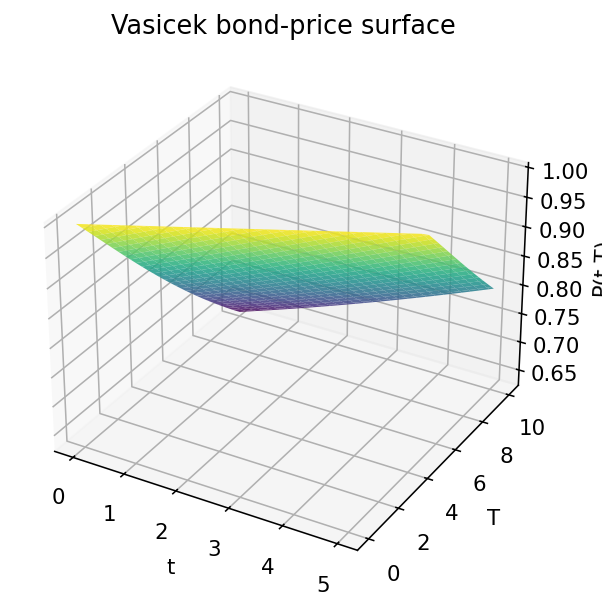
\includegraphics[keepaspectratio]{figures/ch12-bond-surface.png}}
\emph{Vasicek bond-price surface \(P(t,T)\) as a function of the current
short rate and maturity.}

\begin{figure}
\centering
\pandocbounded{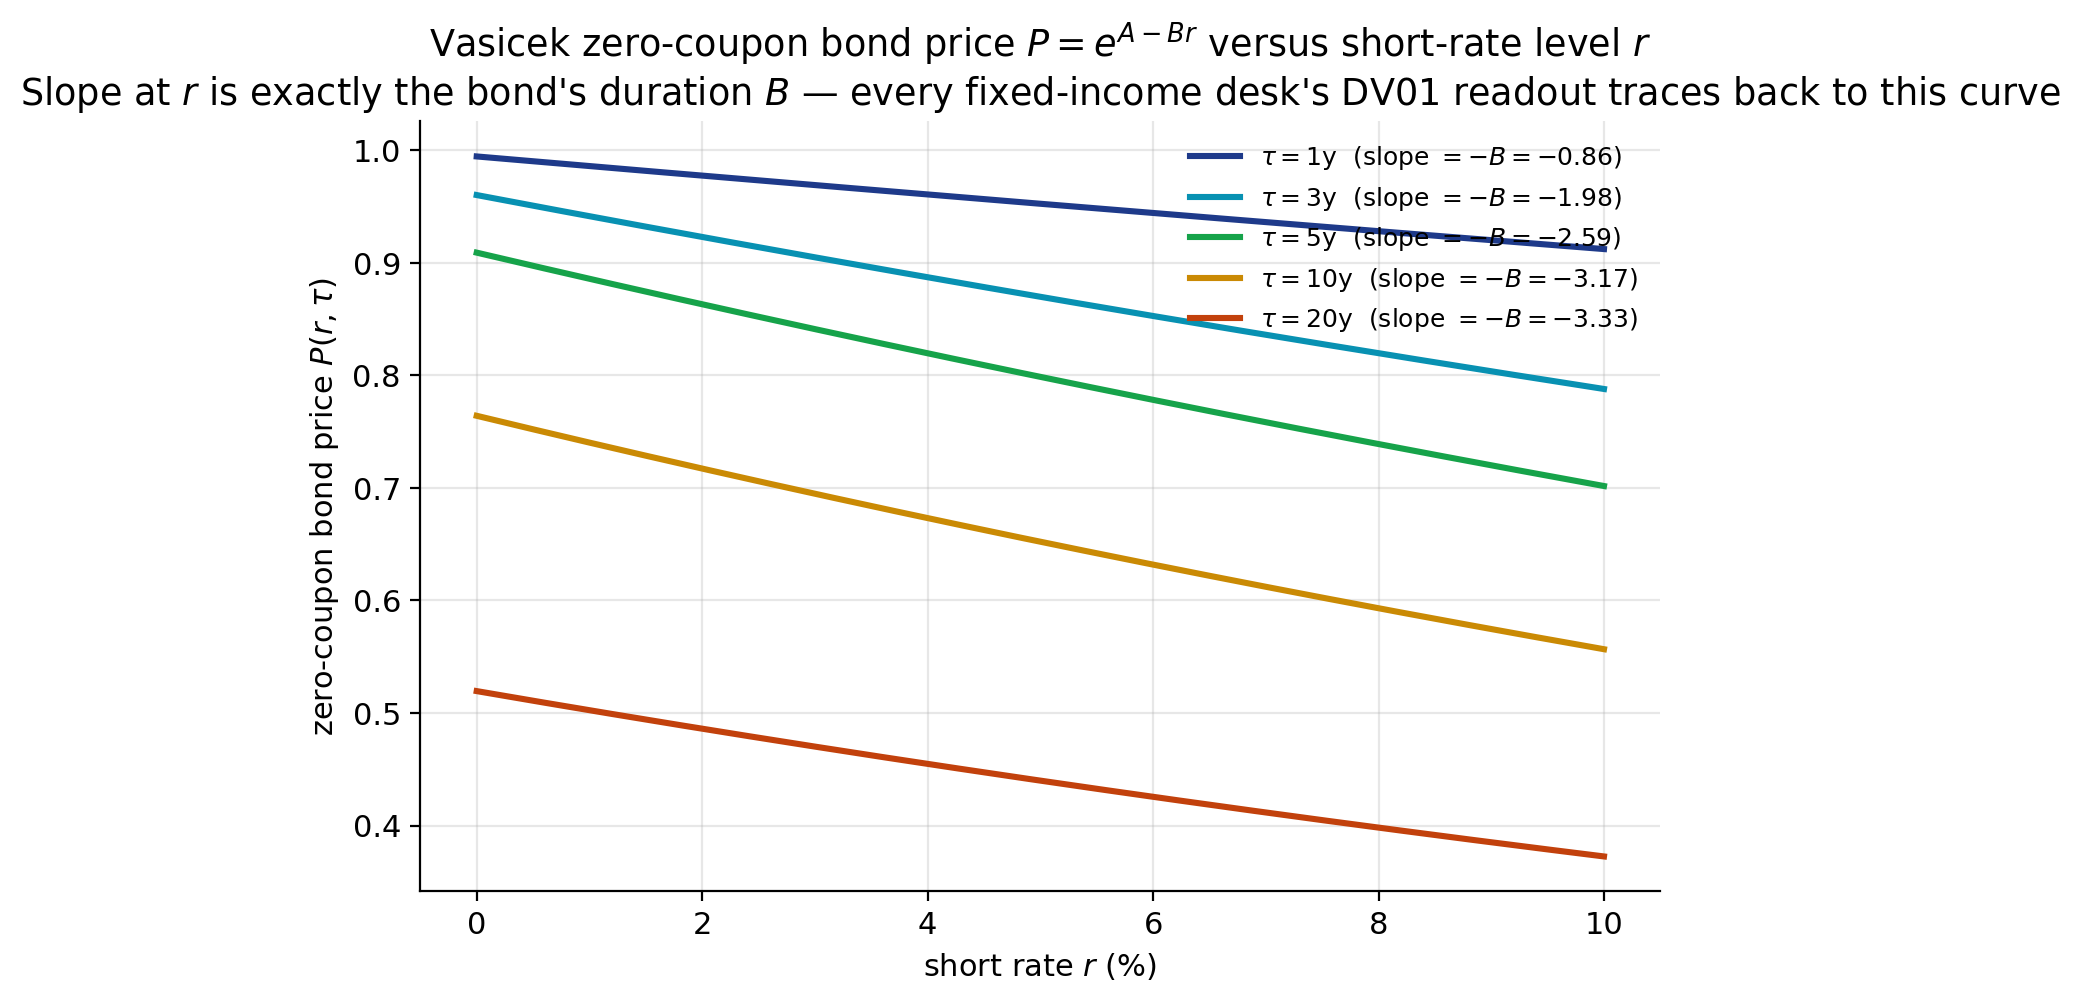
\includegraphics[keepaspectratio]{figures/ch12-bond-vs-rate.png}}
\caption{Vasicek zero-coupon bond price \(P(r, \tau)\) as a function of
\(r\) at several tenors. Slope at each \(r\) equals the Vasicek duration
\(-B(\tau)\) --- the same quantity the desk reports as DV01 per bp of
short-rate shock}
\end{figure}

Let us decode (12.20). The bond price is a log-linear function of the
current short rate: \(\ln P_t(T) = A_t(T) - B_t(T) r_t\). The
coefficient \(B_t(T)\) is the bond's \emph{duration-like} sensitivity:
\(-\partial_{r_t}\ln
P_t(T) = B_t(T)\) is the modified duration with respect to short-rate
shocks. For short maturities (\(T \to t\)), \(B_t(T) \to 0\) and the
bond is insensitive to \(r_t\). For long maturities (\(T \to \infty\)),
\(B_t(T)
\to 1/\kappa\), meaning a very long bond has a finite duration of
\(1/\kappa\) years --- \emph{not} unbounded, because mean reversion caps
the effect. A Vasicek with \(\kappa = 0.1\) (very slow reversion) gives
a long-bond duration of 10 years; with \(\kappa = 0.5\), 2 years. This
is a radically different picture from a random-walk interest rate, under
which long-bond duration would grow without bound.

The finite long-bond duration is one of Vasicek's most distinctive ---
and economically sensible --- predictions. Actual 30-year bonds do not
have three times the sensitivity of 10-year bonds to short-rate moves.
The reason is mean reversion: a short-rate shock today does not
permanently change expected rates fifty years from now --- it is
absorbed by the mean-reverting dynamics over a few \(1/\kappa\) years.
So the marginal duration contribution of each additional year beyond a
few \(1/\kappa\) years is essentially zero. The bond-duration cap at
\(1/\kappa\) is the quantitative expression of this economic insight.

Boundary conditions: \(B_T(T) = 0\), \(A_T(T) = 0\), so \(P_T(T) = 1\).
These encode the defining property of a zero-coupon bond: at maturity it
pays exactly one unit of currency regardless of the state of the
economy.

\pandocbounded{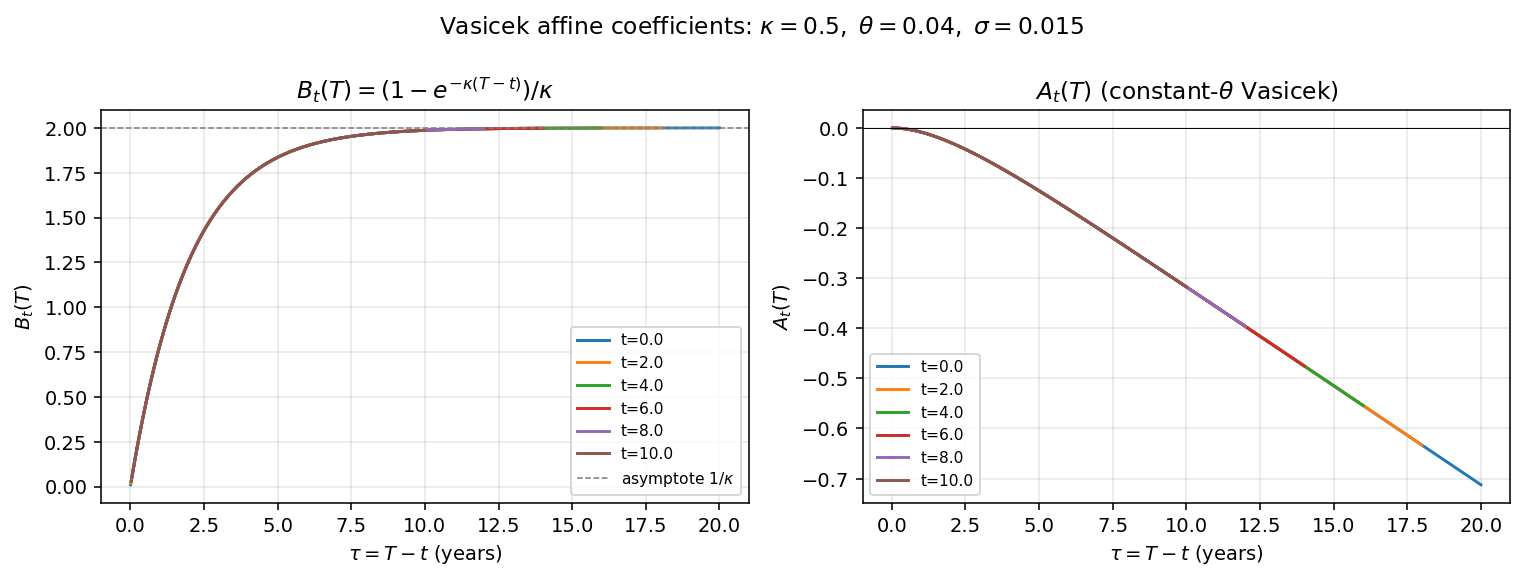
\includegraphics[keepaspectratio]{figures/ch12-affine-coefficients.png}}
\emph{\(B_t(T)\) rises from 0 to the asymptote \(1/\kappa\), encoding
rate sensitivity of long bonds; \(A_t(T)\) is negative and grows in
magnitude with maturity, reflecting the drift and convexity
adjustments.}

\subsection{12.3.5 Affine ansatz and the PDE
route}\label{affine-ansatz-and-the-pde-route}

There is a second, independent route to (12.20) --- and it is the one
that generalises most smoothly to more complex models (CIR,
quadratic-Gaussian, multi-factor affine). Fix \(T\) and view \(P_t(T) =
g(t, r_t)\) as a function of the state \(r_t\). The Feynman-Kac
representation (Chapter 4) says

\[
P_t(T) \;=\; \mathbb{E}^{\mathbb{Q}}_t\!\left[e^{-\int_t^T r_s\,\mathrm{d}s}\right], \quad \mathrm{d}r_t = \kappa(\theta - r_t)\,\mathrm{d}t + \sigma\,\mathrm{d}\widehat{W}_t,
\tag{12.23}
\]

and therefore \(g(t, r)\) satisfies the bond-pricing PDE

\[
\bigl(\partial_t + \mathcal{L}\bigr)\,g(t, r) \;=\; r\,g(t, r), \qquad g(T, r) = 1,
\tag{12.24}
\]

with infinitesimal generator

\[
\mathcal{L} \;=\; \kappa(\theta - r)\,\partial_r + \tfrac{1}{2}\sigma^2\,\partial_{rr}.
\tag{12.25}
\]

Why does the PDE carry a source term \(-rg\) rather than being
sourceless? Because we are not working with discounted prices directly;
we are working with undiscounted bond prices. As time advances by
\(\mathrm{d}t\), the bond's value is reduced by a factor of
\(e^{-r_t\,\mathrm{d}t} \approx 1 - r_t\,\mathrm{d}t\), which
contributes \(-r_t g\,\mathrm{d}t\) to the dynamics. Multiplying \(g\)
by the discount factor \(e^{-\int r}\) would give a process satisfying a
sourceless PDE; the sourced PDE here is for the un-discounted price. A
bond is a traded asset, so its discounted price is a
\(\mathbb{Q}\)-martingale; its undiscounted price is not (it drifts at
\(r_t\)), which is why (12.24) has a non-zero source.

\textbf{Affine ansatz.} Guess

\[
g(t, r) \;=\; e^{A_t - B_t r}, \qquad A_T = 0,\ B_T = 0.
\tag{12.26}
\]

Derivatives: \(\partial_t g = (\dot A_t - \dot B_t r)g\),
\(\partial_r g = -B_t g\), \(\partial_{rr} g = B_t^2 g\). Substitute
into (12.24) and divide by \(g\):

\[
\bigl(\dot A_t - \kappa B_t \theta + \tfrac{1}{2}\sigma^2 B_t^2\bigr) \;+\; \bigl(-\dot B_t + \kappa B_t - 1\bigr)\,r \;=\; 0.
\tag{12.27}
\]

Equation (12.27) is doing something subtle. The left-hand side is a
polynomial in \(r\) of degree one --- an \(r^0\) coefficient and an
\(r^1\) coefficient. For this polynomial to vanish for \emph{all} values
of \(r\), both coefficients must individually be zero. This is the
\emph{matching of coefficients} move, and it is the step that turns one
PDE into two ODEs. It works only because the affine ansatz was the right
guess; had we tried a quadratic ansatz \(\log P = A - Br - Cr^2\), we
would have picked up an \(r^2\) coefficient that did not naturally
vanish, and the ansatz would have failed. The class of models for which
coefficient-matching succeeds is precisely the class of affine models
--- hence the name.

Coefficient matching gives the \emph{affine term-structure ODE system}:

\[
\boxed{\;\;
\begin{cases}
\dot A_t - \kappa B_t\, \theta + \tfrac{1}{2}\sigma^2 B_t^2 \;=\; 0, & \text{(A-ODE)} \\[4pt]
\dot B_t - \kappa B_t + 1 \;=\; 0, & \text{(B-ODE)}
\end{cases}
\qquad A_T = 0,\ B_T = 0. \;\;}
\tag{12.28}
\]

The ODE system (12.28) is structurally beautiful: the \(B\)-equation is
autonomous (involves only \(B\) and constants), while the \(A\)-equation
depends on \(B\) as an input. Solve for \(B\) first, then plug the
result into the \(A\)-equation and integrate. In richer models the
\(B\)-equation becomes a Riccati ODE (quadratic in \(B\)); here in
Vasicek it is merely linear, because the diffusion is constant rather
than state-dependent.

\textbf{Solving B-ODE.} Equation \(\dot B_t - \kappa B_t + 1 = 0\) in
standard form is \(\dot B_t = \kappa B_t - 1\) with \(B_T = 0\).
Integrating factor \(e^{-\kappa t}\) gives

\[
B_t(T) \;=\; \frac{1 - e^{-\kappa(T-t)}}{\kappa},
\tag{12.29}
\]

matching (12.21) exactly. This function depends only on
\(\tau = T - t\), not separately on \(t\) and \(T\) --- a consequence of
the constant-coefficient structure.

\textbf{Solving A-ODE.} Plug \(B_t(T)\) into the \(A\)-ODE and integrate
from \(t\) to \(T\) using \(A_T = 0\):

\[
A_t(T) \;=\; -\!\int_t^T \kappa\, B_s(T)\,\theta\,\mathrm{d}s \;+\; \frac{\sigma^2}{2}\!\int_t^T B_s(T)^2\,\mathrm{d}s.
\tag{12.30}
\]

Substituting \(\kappa B_s(T) = 1 - e^{-\kappa(T-s)}\) and
\(\kappa^2 B_s(T)^2 = (1 - e^{-\kappa(T-s)})^2\), (12.30) becomes
exactly (12.22), providing a cross-check between the two derivation
routes.

The two derivations --- moment-generating-function (§12.3.4) and PDE /
affine ansatz (§12.3.5) --- arrive at the same answer via genuinely
different routes. The former is analytically direct but only works
because Gaussianity makes the MGF explicit. The latter is abstractly
more general (it depends only on affine structure, not on Gaussianity)
and therefore extends to CIR, quadratic-Gaussian models, and affine
jump-diffusions. In research the PDE approach is more often the starting
point because it generalises more cleanly; in pedagogy the
direct-expectation route is more transparent for the Vasicek special
case we are working through.

Some authors prefer yet a third derivation: the martingale-based
approach, where one guesses the bond-price formula and verifies that the
discounted price \(P_t(T)/M_t\) is a martingale under \(\mathbb{Q}\).
This is the most elegant route when it works, because it directly
confirms the no-arbitrage condition rather than deriving the price and
verifying arbitrage-freeness as a corollary. The three approaches ---
expectation, PDE, martingale --- form a triad that characterises
risk-neutral pricing from three complementary angles: operational (how
to compute it), analytic (what equation does it satisfy), and economic
(why is it arbitrage-free). Mastering all three is the mark of a mature
quant.

A more general methodological lesson from this cross-check: in
quantitative finance, having two independent derivations of the same
result is not redundancy --- it is insurance. Each derivation exposes a
different aspect of the mathematical structure, and each is vulnerable
to a different class of errors. The direct-expectation approach is prone
to integration mistakes and Fubini-justification gaps; the PDE approach
is prone to ansatz-guessing errors and boundary-condition confusion.
When both converge on the same formula, one gains high confidence that
neither class of errors has been made.

\section{12.4 The yield curve under
Vasicek}\label{the-yield-curve-under-vasicek}

\subsection{12.4.1 Yields and instantaneous forward
rates}\label{yields-and-instantaneous-forward-rates}

The continuously-compounded yield for maturity \(T\) at time \(t\) is

\[
y_t(T) \;=\; -\,\frac{\ln P_t(T)}{T - t} \;=\; \frac{-A_t(T) + B_t(T)\, r_t}{T - t}.
\tag{12.31}
\]

Yields, not bond prices, are what practitioners and the press typically
quote, so (12.31) is probably the most practically used formula derived
from Vasicek. The conversion from bond prices to yields is conceptually
a simple logarithm-and-divide; the practical utility is that yields are
approximately stationary over long periods, while bond prices drift
toward 1 at maturity.

Under Vasicek, the yield decomposition
\(y_t(T) = -A_t(T)/(T-t) + B_t(T)/(T-t) \cdot r_t\) shows that yields
are themselves affine in \(r_t\). The coefficient \(B_t(T)/(T-t)\) is
the yield's sensitivity to the short rate; it approaches 1 at short
maturities (so short-maturity yields essentially equal \(r_t\)) and
approaches 0 at long maturities (so long-maturity yields are almost
insensitive to \(r_t\), a consequence of mean reversion). The intercept
\(-A_t(T)/(T-t)\) is the ``term-structure contribution'' --- the part of
the yield that does not depend on today's rate.

The instantaneous forward rate at maturity \(T\) is
\(f_t(T) = -\partial_T \ln P_t(T)\). It is the rate at which an investor
could lock in a forward contract today starting at \(T\) for an
infinitesimal period. Equivalently, it is the expected
\(T\)-instantaneous short rate under the \(T\)-forward measure (see
Chapter 13). Bond prices and forward rates are related by
\(\ln P_t(T) = -\int_t^T f_t(s)\,\mathrm{d}s\), and the short rate
itself satisfies \(r_t = f_t(t)\).

A common trap: the forward rate \(f_t(T)\) is \emph{not} in general
equal to the expected future short rate \(\mathbb{E}[r_T]\). Under the
\(T\)-forward measure, \(f_t(T) = \widetilde{\mathbb{E}}^T[r_T]\); under
the risk-neutral measure, \(\mathbb{E}^{\mathbb{Q}}[r_T]\) differs by a
convexity adjustment; under the physical measure, there is an additional
risk-premium correction. When a commentator says ``the market expects
rates to be X\% in five years'' and cites a five-year forward rate, that
statement is true under \(\widetilde{\mathbb{Q}}^5\) but not under
\(\mathbb{P}\) --- and the wedge between them can be substantial,
particularly at longer horizons. Being precise about \emph{which}
measure one is discussing is a hallmark of careful rates analysis.

\subsection{12.4.2 Yield curve shapes}\label{yield-curve-shapes}

For Vasicek:

\begin{itemize}
\tightlist
\item
  As \(T \to t\): \(y_t(T) \to r_t\) (the short rate itself).
\item
  As \(T \to \infty\):
  \(y_t(T) \to \theta - \tfrac{1}{2}\,\sigma^2/\kappa^2\) (the long
  yield --- constant in \(r_t\)).
\item
  In between: the curve can be monotone, humped, or inverted depending
  on \(r_t\) vs \(\theta\).
\end{itemize}

The long-yield limit \(\theta - \tfrac{1}{2}\sigma^2/\kappa^2\) deserves
a pause. The first term, \(\theta\), is the long-run mean of the short
rate --- what you would expect if you simply averaged rates over the
infinite future. The second term is a \emph{subtraction}: the long yield
is \emph{below} the expected long-run short rate. This negative gap is
the convexity premium: because the discount factor is a convex function
of the integrated rate, random variation in future rates raises the
expected discount factor above the deterministic benchmark, and
therefore lowers the implied yield. The magnitude
\(\sigma^2/(2\kappa^2)\) is proportional to the stationary variance of
\(r_t\) --- more volatile or less mean-reverting short rates give larger
convexity premia. This is a genuine economic prediction: in
high-volatility environments, long yields should trade \emph{below}
consensus expectations of the long-run short rate, and the gap should
widen with volatility. Empirically this is reasonably well supported.

Quantifying in a concrete case: with \(\sigma = 0.01\) and
\(\kappa = 0.3\), the premium is
\((0.01)^2/(2 \cdot 0.09) = 5.56 \times 10^{-4}\), or about 5.6 basis
points. With higher volatility \(\sigma = 0.02\) it quadruples to 22 bp.
With slower reversion \(\kappa = 0.15\), the denominator halves-squared
to 0.0225 and the premium is 22.2 bp. So the convexity premium is most
visible in slow-reverting, high-volatility environments --- exactly the
sort of regime that tends to produce inverted or unusually flat yield
curves.

\pandocbounded{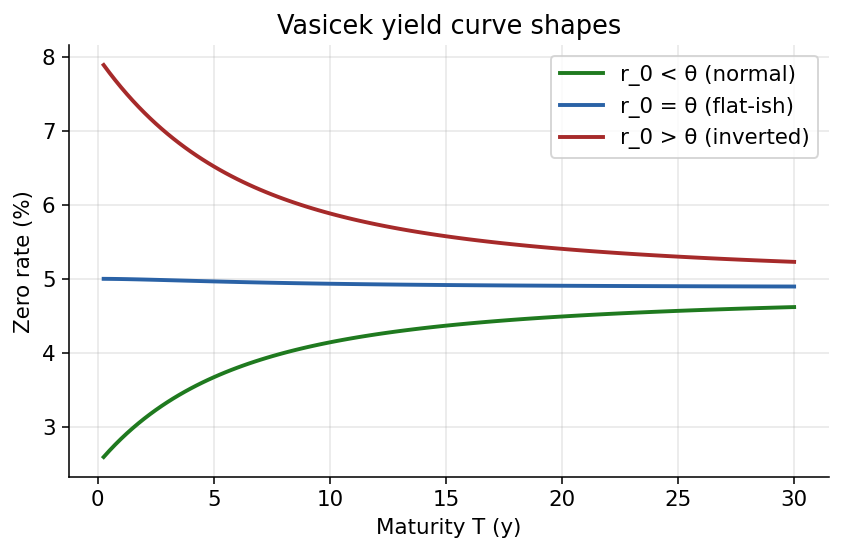
\includegraphics[keepaspectratio]{figures/ch12-vasicek-shapes.png}}
\emph{Vasicek yield-curve shapes for three starting short rates, showing
the classical monotone-rising, humped, and inverted regimes.}

An illustrative calibration. Take \(\kappa = 0.3\), \(\theta = 0.04\),
\(\sigma = 0.015\) and consider three starting rates: \(r_0 \in
\{0.01, 0.04, 0.08\}\). For each compute \(y_0(T)\) across
\(T \in \{1, 2, 5, 10, 30\}\) years.

For \(r_0 = 0.01\) (well below \(\theta\)): the short end is near 1\%,
rises through about 2.5\% at 2 years, 3.2\% at 5, 3.6\% at 10, and
approaches the long-end asymptote \(\theta - \sigma^2/(2\kappa^2) =
0.04 - 0.00125 \approx 3.88\%\) at 30. A monotonically rising curve ---
the classical ``normal'' yield curve in a below-neutral environment.

For \(r_0 = 0.04\) (at \(\theta\)): the curve is nearly flat around
3.9\%, with only the convexity correction producing a slight downward
drift at longer maturities.

For \(r_0 = 0.08\) (well above \(\theta\)): the short end is at 8\%,
falling through about 6.6\% at 2 years, 5.0\% at 5, 4.3\% at 10, and
3.88\% at 30. An inverted curve --- typical of late-cycle monetary
tightening when short rates are elevated but the market expects them to
fall.

These three scenarios show that Vasicek produces economically sensible
curve shapes across the full range of initial conditions, entirely
through the mean-reversion parameter \(\kappa\) and the long-run mean
\(\theta\). The deterministic convergence \(r_t \to \theta\) drives the
shape, and the convexity correction fine-tunes the long end.

\subsection{12.4.3 The 1-factor
limitation}\label{the-1-factor-limitation}

Crucially, all shifts of the curve under Vasicek are driven by a single
factor \(r_t\). Any change in the short rate must propagate through the
\emph{entire} yield curve in a fixed, deterministic way dictated by
\(B_t(T)\). So if the short rate rises by 25 bp, the 2-year yield rises
by some specific amount, the 10-year by another, the 30-year by yet
another --- but the \emph{ratios} among these moves are fixed by the
model. Reality is not so rigid: actual yield-curve moves are dominated
by three roughly orthogonal factors (level, slope, curvature) that move
independently. Principal-components analysis of daily yield-curve
changes consistently shows that three factors explain 95-99\% of the
variance.

To capture this, practitioners turn to multi-factor affine models ---
typically two-factor Hull-White or three-factor affine with independent
Ornstein-Uhlenbeck factors. Each factor contributes its own affine
loading, so a linear combination can match observed yield-curve dynamics
much more faithfully. The cost is higher calibration complexity and more
parameters to stabilise; the benefit is hedges that actually work under
real curve reshapes.

A few common multi-factor specifications deserve mention.

First, the \textbf{two-factor Gaussian model (G2++)}: two independent
(or correlated) Ornstein-Uhlenbeck processes \(x_t\) and \(y_t\), with
the short rate defined as \(r_t = x_t + y_t + \phi(t)\) where
\(\phi(t)\) is a deterministic shift calibrated to today's curve. With
two mean-reversion speeds \(\kappa_x, \kappa_y\) and two volatilities
\(\sigma_x, \sigma_y\) plus a correlation \(\rho\), the model has enough
freedom to match level-plus-slope curve dynamics and a reasonable vol
surface. G2++ is the most widely used multi-factor rates model in
derivative pricing libraries.

Second, the \textbf{three-factor affine model}: three OU factors,
allowing separate calibration to level, slope, and curvature. The
bond-price formula remains exponential-affine in the three-factor state
vector, and the matrix Riccati ODE for \(B(t, T)\) can be solved
explicitly under mild assumptions (diagonal mean-reversion matrix).

Third, the \textbf{Libor Market Model (LMM)}: a radical departure that
models individual forward rates directly rather than a short rate. LMM
can match any yield curve by construction (forward rates are model
inputs, not model outputs) and any swaption vol cube by suitable
specification of forward-rate volatilities and correlations. The price
for this flexibility is giving up the low-dimensional affine structure:
LMM is high-dimensional, state-vector-based, and typically requires
Monte Carlo for complex payoffs.

Which multi-factor model to use is ultimately a portfolio-specific
decision. For vanilla cap-floor-swaption books, G2++ is usually
sufficient. For Bermudan or callable products, LMM or extended affine
models may be needed. For CVA/XVA computations across a huge book, the
calibration speed and hedging accuracy of affine models make them
attractive even when LMM would be ``more accurate'' per trade.

\section{12.5 Ho-Lee --- the canonical
derivation}\label{ho-lee-the-canonical-derivation}

Vasicek with constant \(\theta\) has three parameters \((\kappa, \theta,
\sigma)\) and can fit only three features of a yield curve --- a level,
a slope, and a curvature, roughly. A real observed curve has dozens of
quoted maturities and cannot be reproduced by any three-parameter model.
The natural fix is to let the drift schedule vary with time. The
simplest such extension drops the mean-reversion altogether and retains
only the time-varying drift: this is the Ho-Lee model, which we now
derive from first principles. It serves a dual purpose --- it is
historically the first example of exact yield-curve calibration, and it
is mathematically the \(\kappa \to 0\) limit of Hull-White that we
develop in §12.6.

\subsection{12.5.1 Discrete Ho-Lee}\label{discrete-ho-lee}

The discrete Ho-Lee dynamics on a \(\Delta t\) grid:

\[
\boxed{\;\; r_n \;=\; r_{n-1} \;+\; \theta_{n-1}\,\Delta t \;+\; \sigma\sqrt{\Delta t}\,x_n, \qquad x_n\stackrel{\text{iid}}{\sim}\pm 1\text{ Bernoulli}, \ \mathbb{Q}(x_n = \pm 1) = \tfrac{1}{2}. \;\;}
\tag{12.32}
\]

Read (12.32) aloud: ``tomorrow's short rate equals today's short rate,
plus a deterministic drift over the step, plus a symmetric random
coin-flip scaled to the right standard deviation.'' The drift
\(\theta_{n-1}\) is what curves the rate process to match the market;
the shock \(\sigma\sqrt{\Delta t}\,x_n\) is the noise that lets the rate
move up or down. Because the shock is additive (not multiplicative) and
symmetric, the up-move and down-move at each node have equal magnitude.
This produces a recombining tree --- two steps up and one step down
lands at the same node as one up and two down, reshuffled.

\textbf{Key features.}

\begin{itemize}
\tightlist
\item
  \emph{Arithmetic, not geometric.} Rates are added, not scaled ---
  rates can go negative. Historically this was Ho-Lee's greatest
  weakness; post-2008, actually a feature when pricing negative-rate
  regimes.
\item
  \emph{No mean reversion.} The Ho-Lee dynamic is Vasicek with
  \(\kappa = 0\); only the drift \(\theta_n\) shapes the curve. A pure
  random walk in rates (with drift) means that far out in maturity the
  distribution of \(r_T\) becomes increasingly diffuse and wide.
\item
  \emph{Recombining tree.} With a symmetric \(\pm 1\) shock and constant
  \(\sigma\), up-then-down and down-then-up return to the same node. The
  recombination reduces the node count at step \(n\) from \(2^n\) to
  \(n+1\), making calibration linear-time rather than exponential. This
  is the single largest computational advantage of Ho-Lee and a property
  preserved by its continuous-time limit.
\end{itemize}

\textbf{Calibration goal.} Find \(\theta_0, \theta_1, \theta_2, \ldots\)
so that the model matches the market bond prices \(P_0(1), P_0(2),
P_0(3), \ldots\). The bootstrap is triangular: \(\theta_0\) depends only
on \(P_0(1)\) and \(P_0(2)\), \(\theta_1\) on \(P_0(3)\) given
\(\theta_0\), and so on. We never solve a nonlinear system. At every
step, each new market bond price adds exactly one new equation in
exactly one new unknown \(\theta_n\) --- one of the cleanest pieces of
structure in quantitative finance.

With \(q = 1/2\) inside the tree probability measure, bond prices are

\[
P_0(1) \;=\; e^{-r_0\,\Delta t}, \qquad P_0(2) \;=\; e^{-r_0\Delta t}\!\left[\tfrac{1}{2} e^{-r_{1u}\Delta t} \;+\; \tfrac{1}{2} e^{-r_{1d}\Delta t}\right],
\tag{12.33}
\]

and similarly \(P_0(3)\) depends on \(\theta_0, \theta_1\), giving us
one equation in \(\theta_1\) once \(\theta_0\) is known. The
philosophical takeaway: calibration replaces the abstract non-uniqueness
of \(\mathbb{Q}\) (§12.1.1) with a specific choice of
\(\theta\)-schedule that makes model-implied bond prices equal
market-observed bond prices. Once that schedule is fixed, every other
derivative prices off the resulting tree without further calibration.

\subsection{12.5.2 Continuous-time limit (direct Donsker
argument)}\label{continuous-time-limit-direct-donsker-argument}

The cleanest path to the continuous-time Ho-Lee model: start from
(12.32), sum the recursion, and pass \(N \to \infty\) directly,
bypassing the Vasicek/Hull-White machinery. Fix a horizon \(T\), set
\(\Delta t = T/N\) with \(t_n = n\Delta t\), and iterate (12.32):

\[
r_N \;=\; r_0 \;+\; \sum_{n=1}^{N}\theta_{n-1}\,\Delta t \;+\; \sigma\sqrt{\Delta t}\sum_{n=1}^{N} x_n.
\tag{12.34}
\]

This is a pure telescoping sum: starting level \(r_0\), cumulative
drift, cumulative shock. The moments are immediate:

\[
\mathbb{E}^{\mathbb{Q}}[r_T] \;\to\; r_0 \;+\; \int_0^T \theta_u\,\mathrm{d}u, \qquad \mathbb{V}^{\mathbb{Q}}[r_T] \;=\; \sigma^2 T.
\tag{12.35}
\]

By Donsker's Invariance Principle --- a sum of iid \(\pm 1\) shocks,
scaled by \(\sqrt{\Delta t}\), converges in distribution to Brownian
motion --- we have

\[
\boxed{\;\; r_T \;\stackrel{d}{=}\; r_0 \;+\; \int_0^T \theta_u\,\mathrm{d}u \;+\; \sigma\sqrt{T}\,Z, \qquad Z \sim \mathcal{N}(0, 1), \;\;}
\tag{12.36}
\]

equivalently the SDE

\[
\mathrm{d}r_t \;=\; \theta_t\,\mathrm{d}t \;+\; \sigma\,\mathrm{d}W_t.
\tag{12.37}
\]

The \(\sqrt{\Delta t}\) scaling on the shock is the fundamental scaling
of Brownian motion, which has quadratic variation \(\mathrm{d}t\). Had
we scaled by \(\Delta t\) instead, the limit would have been
deterministic (shock vanishing); by \(1\), it would have been infinite
(shock exploding). The ``right'' scaling \(\sqrt{\Delta t}\) is exactly
what keeps the variance of the sum of \(N\) shocks finite. This scaling
shows up in everything from heat diffusion to stock returns to
interest-rate innovations; it is the signature of a process driven by
``many small independent shocks'' (Chapter 3's construction of Brownian
motion reviews this in detail).

Negative rates are explicit: \(r_T \sim \mathcal{N}(r_0 + \int \theta,
\sigma^2 T)\), so \(\mathbb{P}(r_T < 0) = \Phi(-M/\sqrt{V}) > 0\) where
\(M\) is the mean and \(V\) the variance. For \(T = 10\) years,
\(\sigma = 1\%\), \(M = 3\%\), that probability is \(\Phi(-0.95) \approx
17\%\) --- substantial. For \(T = 1\) year it drops to \(\approx 2\%\).
Negative rates thus bite mainly at long horizons, where variance has had
time to accumulate.

\textbf{Distribution of the integrated rate.} A shock at time \(t\)
affects \emph{all} future \(r_u\) for \(u \in [t, T]\) (the additive
structure with no reversion has infinite memory), contributing with
lever-arm weight \(T - t\) to the integrated rate. Working through the
double-sum calculation,

\[
\int_0^T r_u\,\mathrm{d}u \;\stackrel{d}{=}\; r_0\,T \;+\; \int_0^T\!\int_0^u \theta_s\,\mathrm{d}s\,\mathrm{d}u \;+\; \left(\frac{\sigma^2 T^3}{3}\right)^{\!1/2}\!Z.
\tag{12.38}
\]

The cubic growth \(T^3/3\) of the variance --- as opposed to \(T\) for
the process itself --- is Ho-Lee's signature of missing mean reversion.
Physically: \(\text{Var}[\int_0^T r_u\,\mathrm{d}u] = \int_0^T (T -
t)^2\,\mathrm{d}t \cdot \sigma^2 = \sigma^2 T^3/3\). A 30-year Ho-Lee at
\(\sigma = 1\%\) would give \(\sigma^2 T^3/3 = 10^{-4} \cdot
9000 = 0.9\), an integrated-rate standard deviation of 94\%. This is
absurdly large --- translated into bond-price uncertainty, it implies
extreme price sensitivity to model parameters at long horizons. Mean
reversion (Vasicek/HW) fixes this by making variance grow only linearly
in \(T\) at long horizons. This is the single biggest practical reason
Ho-Lee is rarely used for long-dated instruments.

\subsection{\texorpdfstring{12.5.2.b The meaning of the
\(\sqrt{\Delta t}\)
scaling}{12.5.2.b The meaning of the \textbackslash sqrt\{\textbackslash Delta t\} scaling}}\label{b-the-meaning-of-the-sqrtdelta-t-scaling}

The scaling \(\sqrt{\Delta t}\) on the shock is not arbitrary. Brownian
motion was first introduced by Einstein (1905) to model pollen grains in
water --- particles buffeted by countless small random molecular
collisions. Einstein's analysis showed that for such a process, the
position's variance grows linearly in time: \(\mathbb{V}[X_t] \propto
t\). Linear variance growth in continuous time translates to
\(\sqrt{\Delta t}\) scaling of discrete increments (because variance of
a sum of \(N\) independent increments equals \(N\) times the
per-increment variance, and if \(N\) times some number equals \(T\),
then the per-increment standard deviation is
\(\sqrt{T/N} = \sqrt{\Delta t}\)). This scaling shows up in heat
diffusion, stock returns, interest-rate innovations, and countless other
physical processes. It is the signature of ``many small independent
shocks.''

The \(\sqrt{\Delta t}\) scaling also underpins the famous quadratic-
variation result: \((\mathrm{d}W_t)^2 = \mathrm{d}t\) in the
Itô-calculus limit. This is not an equality in the ordinary sense (both
sides are random) but a precise statement about how squared
infinitesimal increments behave in \(L^2\). That \((\mathrm{d}W_t)^2\)
is deterministic (equal to \(\mathrm{d}t\)) is the reason Brownian
calculus has its peculiar features --- Itô's lemma includes a
second-order term proportional to variance, reflecting the nonzero
quadratic variation. In rate pricing, this shows up as the convexity
term \(C_T\); in equity pricing, as the extra \(\frac{1}{2}\sigma^2\)
drift in the geometric- Brownian solution.

If we relax the ``finite variance'' constraint and allow shocks to have
heavy tails with infinite variance, the limit becomes a stable Lévy
process instead of Brownian motion. Stable Lévy processes have jumps;
they are discontinuous. This is the mathematical basis for jump-
diffusion models of rates, equity prices, and credit spreads. Such
models are sometimes used when heavy tails are important (e.g. pricing
equity index options during tail events), but they are not standard for
rates. The Gaussian limit is the default because it matches observed
rate-change distributions reasonably well at the level of daily moves,
and the mathematical benefits are substantial.

\subsection{12.5.3 Bond price and calibration under continuous
Ho-Lee}\label{bond-price-and-calibration-under-continuous-ho-lee}

Because \(I_T = \int_0^T r_u\,\mathrm{d}u\) is Gaussian,
\(\mathbb{E}^{\mathbb{Q}}[e^{-I_T}] = \exp(-\mathbb{E}I_T +
\tfrac{1}{2}\mathbb{V}I_T)\), giving

\[
\boxed{\;\; \ln P_0(T) \;=\; -r_0\,T \;-\; \int_0^T\!\int_0^u \theta_s\,\mathrm{d}s\,\mathrm{d}u \;+\; \frac{\sigma^2 T^3}{6}. \;\;}
\tag{12.39}
\]

The \(+\sigma^2 T^3/6\) is the Ho-Lee convexity adjustment. Read in
context of (12.19): \(+\tfrac{1}{2}\Sigma_*^2 = +\tfrac{1}{2}\sigma^2
T^3/3 = \sigma^2 T^3/6\) --- Jensen's mountain applied to a cubically
growing variance.

\textbf{Calibration via differentiation.} Since (12.39) expresses \(\ln
P_0(T)\) as a double integral of \(\theta\) plus known terms,
differentiating twice with respect to \(T\) pulls out \(\theta_T\)
pointwise.

First derivative:

\[
\partial_T \ln P_0^*(T) \;=\; -r_0 \;-\; \int_0^T \theta_s\,\mathrm{d}s \;+\; \frac{\sigma^2 T^2}{2}.
\tag{12.40}
\]

Since \(\partial_T \ln P_0^*(T) = -f_0(T)\), this rearranges to the
Ho-Lee forward-curve identity \(f_0(T) = r_0 + \int_0^T \theta_s\,
\mathrm{d}s - \sigma^2 T^2/2\).

Second derivative:

\[
\partial_T^2 \ln P_0^*(T) \;=\; -\theta_T \;+\; \sigma^2 T,
\tag{12.41}
\]

and therefore

\[
\boxed{\;\; \theta_T \;=\; -\,\partial_T^2 \ln P_0^*(T) \;+\; \sigma^2 T. \;\;}
\tag{12.42}
\]

Equation (12.42) is the classical Ho-Lee calibration identity. Read it
intuitively: the drift target \(\theta_T\) at time \(T\) is ``the slope
of the forward curve'' plus ``a convexity bump proportional to \(T\).''
If the forward curve is flat, the drift target is just the convexity
bump. If the forward curve is rising, \(\theta_T\) is positive and the
model drifts rates upward on average.

In practice one fits a smooth parametric form (Nelson-Siegel, Svensson,
cubic splines) to the observed log-bond curve, differentiates the fit
twice, adds the convexity bump, and reads off \(\theta_T\) at every grid
point. The choice of curve-smoother affects the resulting \(\theta(t)\)
qualitatively: noisy second derivatives translate into noisy
\(\theta(t)\), which makes the rate model unstable and gives erratic
prices for non-calibration instruments.

\subsection{\texorpdfstring{12.5.4 Ho-Lee as the \(\kappa \to 0\) limit
of
Hull-White}{12.5.4 Ho-Lee as the \textbackslash kappa \textbackslash to 0 limit of Hull-White}}\label{ho-lee-as-the-kappa-to-0-limit-of-hull-white}

Ho-Lee is precisely the \(\kappa = 0\) specialisation of the Hull-White
dynamics (below):

\[
\underbrace{\mathrm{d}r_t = \kappa(\theta_t - r_t)\,\mathrm{d}t + \sigma\,\mathrm{d}W_t}_{\text{Hull-White}}
\xrightarrow{\kappa \to 0}
\underbrace{\mathrm{d}r_t = \theta_t\,\mathrm{d}t + \sigma\,\mathrm{d}W_t}_{\text{Ho-Lee}}
\]

with the understanding that the Hull-White \(\theta_t\) must diverge as
\(1/\kappa\) for the limit to be well-defined --- the joint limit
\(\kappa\theta_t \to \theta_{\text{HL}}\) is what survives. Conceptually
the three models nest: Ho-Lee is the simplest thing; Vasicek adds a
pull-to-constant-target; Hull-White makes that target time-varying. The
calibration machinery for Hull-White specialises to Vasicek (constant
\(\theta\)) and to Ho-Lee (\(\kappa = 0\)) with minimal changes. This
pedagogical nesting is why we present them in this order.

\section{12.6 Hull-White --- the canonical
derivation}\label{hull-white-the-canonical-derivation}

Vasicek captures mean reversion but has only a constant \(\theta\), so
it can fit only a single feature of the observed term structure
(roughly, the long-run mean). Ho-Lee captures exact yield-curve matching
but has no mean reversion, so its variance grows cubically and the model
breaks at long horizons. Hull-White is the best of both worlds: Vasicek
dynamics with a \emph{time-dependent} drift target \(\theta(t)\). The
function \(\theta(t)\) is calibrated so the model exactly reproduces
today's yield curve, while the mean-reversion parameter \(\kappa\) tames
variance growth.

\subsection{12.6.1 Discrete Hull-White}\label{discrete-hull-white}

Promote the constant \(\theta\) in (12.9) to a deterministic function
\(\theta_t\) and replace \(\pm 1\) Bernoullis with Gaussian innovations:

\[
\boxed{\;\; r_{t_n} - r_{t_{n-1}} \;=\; \kappa\bigl(\theta_{t_{n-1}} - r_{t_{n-1}}\bigr)\,\Delta t \;+\; \sigma\sqrt{\Delta t}\,\chi_n, \qquad \chi_n \stackrel{\text{iid}}{\sim} \mathcal{N}(0, 1). \;\;}
\tag{12.43}
\]

The move from constant \(\theta\) to time-varying \(\theta(t)\) is the
conceptual leap. In Vasicek the process always reverts toward the same
number, so you can only fit one long-run level. In Hull-White the
process reverts toward a \emph{moving target} --- the target itself is a
calibrated function of time --- so every part of the yield curve can be
independently matched. The price is infinite-dimensional calibration
(one \(\theta\) per time point), but as we will see this reduces to a
linear bootstrap exactly as in Ho-Lee.

\textbf{What the parameters mean.}

\begin{itemize}
\tightlist
\item
  \(\kappa\) is a \emph{speed}: the deterministic part of (12.43) pulls
  \(r\) toward \(\theta_t\) at exponential rate \(\kappa\). Large
  \(\kappa \Rightarrow\) very ``sticky'' short rate around \(\theta\);
  small \(\kappa \Rightarrow\) near-random-walk (Ho-Lee). Typical
  calibrated values live in 0.05-0.3 per year, giving shock half-lives
  of 2-15 years.
\item
  \(\sigma\) sets the innovation scale. The unconditional variance of
  \(r_T\) approaches \(\sigma^2/(2\kappa)\) as \(T \to \infty\). Typical
  \(\sigma\) values are 0.005-0.02 in absolute rate terms (50-200 bp per
  year root-volatility).
\item
  \(\theta(t)\) is the \emph{drift shaper}: the knob tuned to the
  market. In the limit it is essentially
  \(f_0(t) + \sigma^2 \cdot(\text{convexity})\), where \(f_0(t)\) is the
  instantaneous forward rate.
\end{itemize}

It is worth pausing on the division of labour. \(\kappa\) and \(\sigma\)
are the \emph{volatility-structure} parameters --- they determine how
rates move, how persistent shocks are, how volatile caps and swaptions
will be. These are typically calibrated \emph{jointly} against
vol-sensitive instruments (ATM swaption prices). \(\theta(t)\) is the
\emph{curve-fitting} parameter, chosen conditionally on
\((\kappa, \sigma)\) to exactly match the discount curve. So calibration
has two stages: first pick \((\kappa,
\sigma)\) to match vol-sensitive instruments, then bootstrap
\(\theta(t)\) to match bond prices. This two-stage structure is
characteristic of rates calibration in practice.

In production systems the two stages are often iterated. A first pass
with historically-sensible \((\kappa, \sigma)\) produces a \(\theta(t)\)
schedule. The resulting model is then used to price a set of swaptions,
and the \((\kappa, \sigma)\) are adjusted to reduce swaption-price
errors. Then \(\theta(t)\) is re-bootstrapped with the updated
\((\kappa, \sigma)\), and so on until convergence. The inner bootstrap
(curve) takes microseconds; the outer optimisation (swaption fit) takes
seconds to minutes. The separation of concerns is crucial: the fast
bootstrap runs inside the slow optimiser.

\pandocbounded{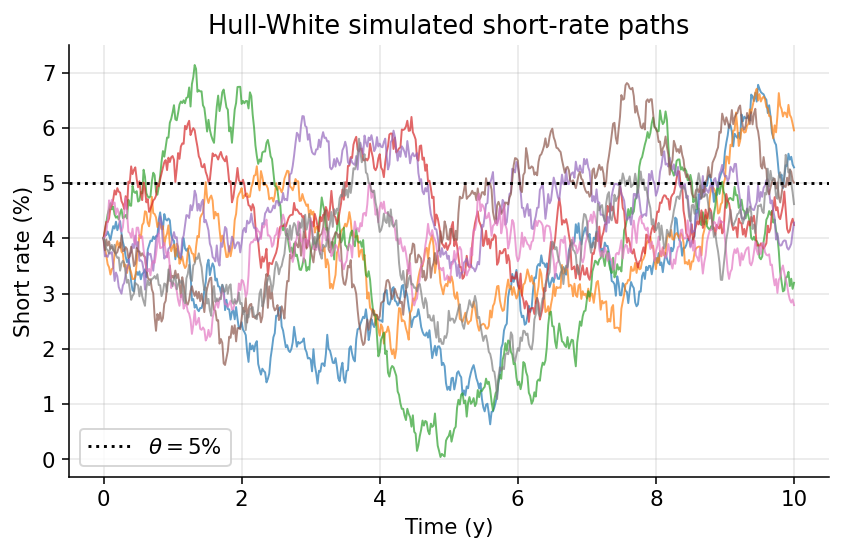
\includegraphics[keepaspectratio]{figures/ch12-hw-paths.png}}
\emph{Hull-White simulated short-rate paths reverting to time-dependent
\(\theta(t)\).}

\subsection{12.6.2 Summed integral and continuous
limit}\label{summed-integral-and-continuous-limit}

Unrolling (12.43) recursively with \(\beta = 1 - \kappa\Delta t\) and
\(\alpha_{n-1} = \kappa\theta_{t_{n-1}}\Delta t\) yields the same
geometric structure as the Vasicek unrolling, with the single difference
that the intercept \(\alpha\) varies with \(n\):

\[
r_T \;=\; r_0\,\beta^N \;+\; \sum_{n=1}^N \alpha_{n-1}\,\beta^{N-n} \;+\; \sigma\sqrt{\Delta t}\sum_{n=1}^N x_n\,\beta^{N-n}.
\tag{12.44}
\]

Taking \(N \to \infty\) with \(\Delta t = T/N\), the standard
Donsker-type identifications give:

\begin{itemize}
\tightlist
\item
  \((1 - \kappa T/N)^{N-n} \to e^{-\kappa(T-u)}\),
\item
  \((1 - \kappa T/N)^N \to e^{-\kappa T}\),
\item
  \(\sum_n (\cdot)\,\Delta t \to \int_0^T (\cdot)\,\mathrm{d}u\),
\item
  \(\sigma\sqrt{\Delta t}\sum_n x_n\,\beta^{N-n} \to \sigma\int_0^T
  e^{-\kappa(T-u)}\,\mathrm{d}W_u\).
\end{itemize}

Each of these is a standard stochastic-calculus limit (Chapter 3): the
first two use \(\lim_N(1 + x/N)^N = e^x\); the third is the
Riemann-sum-to-integral limit; the fourth is Itô's stochastic-integral
construction for a deterministic integrand.

The Wiener integral \(\int_0^T e^{-\kappa(T-u)}\,\mathrm{d}W_u\) is a
Gaussian random variable with mean zero and variance
\(\int_0^T e^{-2\kappa(T-u)}\,\mathrm{d}u = (1 -
e^{-2\kappa T})/(2\kappa)\) --- exactly the Vasicek stationary-variance
formula. This clean Gaussian structure is the source of the closed-form
bond price. Had the integrand been state-dependent (like \(\sqrt{r_u}\)
in CIR), the integral would be a true Itô integral, not a Wiener
integral, and its distribution would not be Gaussian.

The limit of (12.44) is the explicit Hull-White solution:

\[
r_T \;=\; r_0\,e^{-\kappa T} \;+\; \kappa\!\int_0^T e^{-\kappa(T-u)}\,\theta_u\,\mathrm{d}u \;+\; \sigma\!\int_0^T e^{-\kappa(T-u)}\,\mathrm{d}W_u.
\tag{12.45}
\]

The pattern is identical to Vasicek with constant \(\theta\) (equation
(12.12)); only the deterministic drift contribution has been generalised
from a function of \(\tau = T - t\) alone to a true integral against the
time-varying \(\theta_u\).

\subsection{12.6.3 Hull-White bond price}\label{hull-white-bond-price}

The integrated rate, by the same Fubini manipulation as in §12.3.3:

\[
\int_0^T r_u\,\mathrm{d}u \;=\; r_0\,B_T \;+\; A_T \;+\; \frac{\sigma}{\kappa}\!\int_0^T\!\bigl(1 - e^{-\kappa(T-u)}\bigr)\,\mathrm{d}W_u,
\tag{12.46}
\]

where

\[
B_T \;=\; \frac{1 - e^{-\kappa T}}{\kappa}, \qquad A_T \;=\; \int_0^T \theta_u\,\bigl(1 - e^{-\kappa(T-u)}\bigr)\,\mathrm{d}u.
\tag{12.47}
\]

\(B_T\) is worth a moment because it is the single most-used quantity in
Hull-White computations: the ``effective duration'' that the current
short rate \(r_0\) exerts on the integrated rate. In the
\(\kappa \to 0\) limit, \(B_T \to T\) (no reversion means the current
rate affects the entire horizon). In the \(\kappa \to \infty\) limit,
\(B_T \to 0\) (infinite reversion instantly forgets the current rate).
For typical \(\kappa \in [0.05, 0.3]\), the ratio \(B_T/T\) ranges from
near 1 at short \(T\) down to something much smaller at long \(T\). For
\(\kappa =
0.15\) and \(T = 30\): \(B_T = (1 - e^{-4.5})/0.15 \approx 6.6\), so
\(B_T/T \approx 0.22\). The current rate has 22\% as much influence on
the 30-year bond price as it would under no mean reversion.

Because the integrated rate is Gaussian with mean \(r_0 B_T + A_T\) and
variance

\[
\mathbb{V}\!\left[\int_0^T r_u\,\mathrm{d}u\right] \;=\; \frac{\sigma^2}{\kappa^2}\!\int_0^T\!\bigl(1 - e^{-\kappa(T-u)}\bigr)^2\,\mathrm{d}u \;\equiv\; 2\,C_T,
\tag{12.48}
\]

the Hull-White bond price comes out directly from the Gaussian
moment-generating function:

\[
\boxed{\;\; P_0(T) \;=\; \exp\!\left\{-r_0\,B_T \;-\; A_T \;+\; C_T\right\}, \;\;}
\tag{12.49}
\]

with convexity adjustment

\[
C_T \;=\; \frac{\sigma^2}{2\kappa^2}\!\int_0^T\!\bigl(1 - e^{-\kappa(T-u)}\bigr)^2\,\mathrm{d}u.
\tag{12.50}
\]

Reading (12.49), three pieces:

\begin{itemize}
\tightlist
\item
  \(r_0 B_T\): current-level contribution, decaying at rate \(\kappa\)
  because a rate shock ``today'' is damped over the life of the bond.
\item
  \(A_T\): the drift contribution from the \(\theta\) path. All the
  market information about future forward rates lives here.
\item
  \(+C_T\): positive convexity. Jensen's inequality makes the bond
  strictly \emph{more} valuable than naive plug-in discounting suggests.
  This is the Hull-White analogue of the \(\sigma^2 T^3/6\) term in
  Ho-Lee and of the \(\tfrac{1}{2}\Sigma_*^2\) term in
  constant-\(\theta\) Vasicek.
\end{itemize}

\textbf{Sanity checks.} As \(\kappa \to 0\) (Taylor-expanding \((1 -
e^{-\kappa(T-u)})^2 \approx \kappa^2(T-u)^2\)), we have \(B_T \to T\),
\(A_T \to \int_0^T \theta_u\,\mathrm{d}u\), and \(C_T \to \sigma^2
T^3/6\). Formula (12.49) collapses to the Ho-Lee formula (12.39).
Setting \(\theta(t) = \theta\) constant, \(A_T = \theta(T - B_T)\) and
(12.49) specialises to Vasicek. The nesting is clean and complete:
Ho-Lee \(\subset\) Vasicek \(\subset\) Hull-White.

The \(\kappa^2\) cancellation in the \(C_T\) limit is a specific
instance of a more general phenomenon: many quantities in Hull-White
approach their Ho-Lee limits smoothly as \(\kappa \to 0\), because the
mean-reversion structure enters quadratically in the variance terms and
linearly in the mean terms. This smoothness of limits lets us calibrate
Vasicek/Hull-White parameters to low \(\kappa\) values without numerical
difficulty.

\textbf{Worked magnitude.} For \(T = 10\), \(\sigma = 0.01\),
\(\kappa = 0.1\): the integral
\(\int_0^{10}(1 - e^{-0.1(10-u)})^2\,\mathrm{d}u = 10 -
2(1 - e^{-1})/0.1 + (1 - e^{-2})/0.2 = 10 - 12.64 + 4.32 = 1.68\), so
\(C_{10} = (10^{-4}/0.02)\cdot 1.68 = 0.0084\) --- an 84-bp bonus in
log-bond. By comparison, Ho-Lee with the same \(\sigma\) at \(T = 10\)
gives \(C_{10} = \sigma^2 T^3/6 = 0.0167\), or 167 bp --- roughly
double. Mean reversion halves the 10-year convexity bonus and the gap
grows exponentially at longer tenors. At \(T = 30\) the Ho-Lee number is
\(\sigma^2 T^3/6 = 0.45\) (4500 bp!) while Hull-White (\(\kappa = 0.1\))
comes in around 600 bp --- an order of magnitude smaller. This is why
mean reversion matters for long-dated pricing: Ho-Lee's unbounded
convexity growth is unrealistic; Hull-White's bounded growth matches
market observations.

\pandocbounded{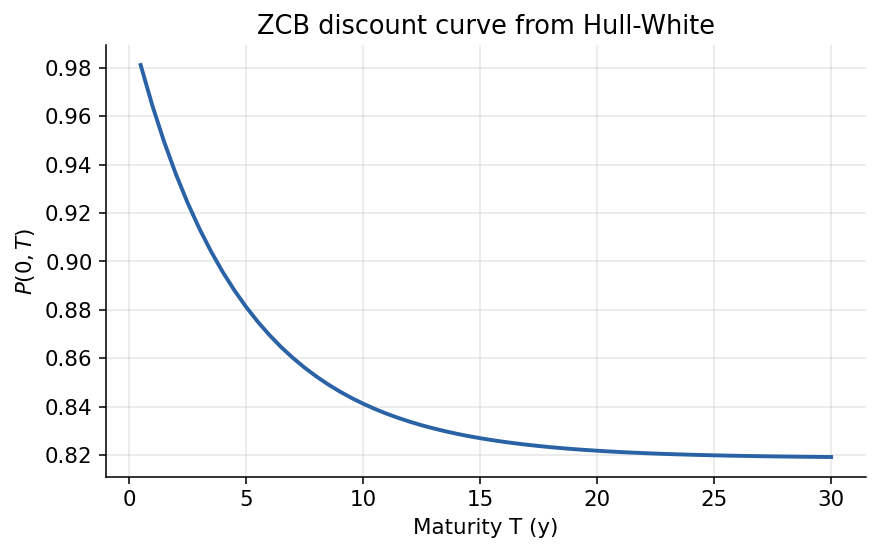
\includegraphics[keepaspectratio]{figures/ch12-zcb-curve.png}}
\emph{Model-implied zero-coupon bond / discount curve \(P_0(T)\).}

\subsection{12.6.3.b Precomputation and numerical
considerations}\label{b-precomputation-and-numerical-considerations}

For pricing efficiency it is convenient to precompute the ``basis
functions'' once per maturity \(T\): \(1 - e^{-\kappa(T-t)}\),
\((T-t) - B_t(T)\), and
\((T-t) - 2B_t(T) + (1 - e^{-2\kappa(T-t)})/(2\kappa)\). Then \(A_t(T)\)
and \(B_t(T)\) are simple linear combinations with coefficients
\(\theta\), \(\sigma^2/(2\kappa^2)\), etc. In production rates
libraries, the ODEs for \(A\) and \(B\) are solved once at
model-initialisation time and cached; during pricing, the pre-computed
\(A(t, T)\) and \(B(t, T)\) are simply evaluated at the appropriate
\((t, T)\) pair. This makes bond pricing essentially instantaneous --- a
table lookup rather than an integration. The same caching strategy
applies to multi-factor affine models and is part of why these models
scale so gracefully to large trading books.

The finite long-bond duration \(1/\kappa\) is the quantitative
expression of mean reversion. \emph{Caveat: this is a model artefact of
Vasicek with constant \(\theta\), not an empirical fact.} The bound says
that under the model's dynamics --- exponential mean reversion of the
short rate to a constant target --- the bond-price sensitivity to
\(r_0\) asymptotes at \(1/\kappa\) years. Empirical 30-year Treasury
modified durations run \(15\)--\(20\) years, well above the
\(2\)--\(10\) year window that ``reasonable'' \(\kappa \in [0.1, 0.5]\)
produces. The discrepancy is resolved by Hull-White's time-varying
\(\theta(t)\): with a calibrated \(\theta\) schedule the model
reproduces empirical duration without forcing \(\kappa\) outside the
volatility-instrument-implied range. A calibration algorithm returning
\(\kappa\) outside \([0.1, 0.5]\) under \emph{constant-\(\theta\)}
Vasicek is a flag of model mis-specification, not an empirical truth
about rates.

\subsection{\texorpdfstring{12.6.4 Calibrating \(\theta(u)\) to the
market
curve}{12.6.4 Calibrating \textbackslash theta(u) to the market curve}}\label{calibrating-thetau-to-the-market-curve}

In practice one observes market bond prices \(P_0^*(T)\) (or yields) at
\(t = 0\) for all maturities \(T\). The idea of Hull-White: choose the
deterministic function \(\theta_t\) so the model reproduces \(P_0^*(T)\)
exactly. Why is this so important? Because a rates trader using a model
that doesn't match today's curve is effectively betting that today's
market is mispriced --- almost never a useful default. With
\(\theta(t)\) free, the model has enough functional freedom to fit any
observed curve exactly; the remaining parameters \((\kappa, \sigma)\)
are then fit to options on bonds.

From (12.49), taking logs at \(t = 0\),

\[
\ln P_0^*(T) \;=\; -r_0\,B_T \;-\; \int_0^T \theta_u\,\bigl(1 - e^{-\kappa(T-u)}\bigr)\,\mathrm{d}u \;+\; C_T.
\tag{12.51}
\]

\textbf{Closed-form inversion.} Differentiating twice in \(T\) gives the
pointwise Hull-White calibration identity:

\[
\boxed{\;\; \theta(T) \;=\; \frac{1}{\kappa}\,\partial_T f_0(T) \;+\; f_0(T) \;+\; \frac{\sigma^2}{2\kappa^2}\!\left(1 - e^{-2\kappa T}\right), \;\;}
\tag{12.52}
\]

where \(f_0(T) = -\partial_T \ln P_0^*(T)\) is the market instantaneous
forward rate. The first term is the slope of the forward curve scaled by
\(1/\kappa\), the second is a level match to the forward itself, and the
third is a maturity-dependent convexity adjustment that saturates at
\(\sigma^2/(2\kappa^2)\) for large \(T\). In the \(\kappa \to 0\) limit,
\(\kappa\,\theta(T)\) --- not \(\theta(T)\) itself --- must remain
finite (see §12.5.4): multiplying (12.52) through by \(\kappa\) gives
\(\kappa\theta(T) = \partial_T f_0(T) + \kappa f_0(T) +
(\sigma^2/2\kappa)(1-e^{-2\kappa T})\), and taking \(\kappa \to 0\) the
middle term vanishes while the last approaches \(\sigma^2 T\), so
\(\kappa\theta \to \partial_T f_0 + \sigma^2 T = \theta_{\text{HL}}\),
recovering the Ho-Lee formula (12.42).

\textbf{Bucket bootstrap.} In implementation, (12.52) is rarely used
literally because it requires a second derivative of the observed
forward curve, which is numerically ill-conditioned. Production
implementations parameterise \(\theta(t)\) as piecewise constant on the
bond-maturity grid, and solve for the parameter values that exactly
reproduce observed bond prices. Splitting the integral in (12.51) into
bucket contributions with piecewise-constant \(\theta^{(m)}\) on
\([T_{m-1}, T_m]\):

\[
A_{T_k} \;=\; \sum_{m=1}^k \theta^{(m)}\,\alpha^{(m, k)}, \qquad \alpha^{(m, k)} \;=\; (T_m - T_{m-1}) \;-\; \frac{e^{-\kappa(T_k - T_m)} - e^{-\kappa(T_k - T_{m-1})}}{\kappa}.
\tag{12.53}
\]

Solving (12.51) for the current bucket \(\theta^{(k)}\) yields the
bootstrap recursion:

\[
\boxed{\;\; \theta^{(k)} \;=\; \frac{T_k\, y_k^* \;-\; r_0\, B_{T_k} \;+\; C_{T_k} \;-\; \sum_{m=1}^{k-1}\theta^{(m)}\,\alpha^{(m, k)}}{\alpha^{(k, k)}}. \;\;}
\tag{12.54}
\]

This is a simple linear bootstrap, exactly analogous to Ho-Lee and to
yield-curve stripping: each tenor \(T_k\) determines \(\theta^{(k)}\)
given the already-calibrated earlier buckets. No optimisation, no
iteration, no nonlinearity. Just a sequence of divisions.

The \(\alpha^{(m, k)}\) are ``overlap weights'' --- how much of bucket
\(m\)'s drift influences the integrated rate up to horizon \(T_k\). They
are pure geometry of the exponential kernel and do not depend on market
data; production implementations precompute them once per \(\kappa\) and
cache. Their key property is causality: \(\alpha^{(m, k)} = 0\) for
\(m > k\), which is what makes the bootstrap triangular. A
\(\theta^{(m)}\) for \(m > k\) has no effect on \(P_0(T_k)\) (it refers
to rates in the future relative to \(T_k\)), so adding tenor \(T_k\)
determines only \(\theta^{(k)}\) and leaves earlier buckets fixed.

\textbf{Worked example.} Take \(\kappa = 0.15\), \(\sigma = 0.012\),
\(r_0 =
0.04\), market yields \(y_1^* = 0.042\) at \(T_1 = 1\) and \(y_2^* =
0.045\) at \(T_2 = 2\). Compute \(B_{T_1} = (1 - e^{-0.15})/0.15 \approx
0.9286\) and \(C_{T_1} \approx 3.4 \times 10^{-5}\). With \(k = 1\) the
sum is empty and \(\alpha^{(1, 1)} = T_1 - B_{T_1} \approx 0.0714\).
Then

\[
\theta^{(1)} \;\approx\; \frac{1 \cdot 0.042 - 0.04 \cdot 0.9286 + 3.4\mathrm{e}{-5}}{0.0714} \;\approx\; 0.0691.
\]

The calibrated drift target is about 6.9\% --- well above the current
4\% level. This is the ``overshoot'': mean reversion only partially
converges the rate toward \(\theta^{(1)}\) over one year
(\(\mathbb{E}[r_1] = 0.04 \cdot e^{-0.15} + \theta^{(1)}(1 -
e^{-0.15}) \approx 0.04 \cdot 0.861 + \theta^{(1)} \cdot 0.139\)), so
\(\theta^{(1)}\) must overshoot the target rate level to achieve the
market-implied integrated-rate value.

\pandocbounded{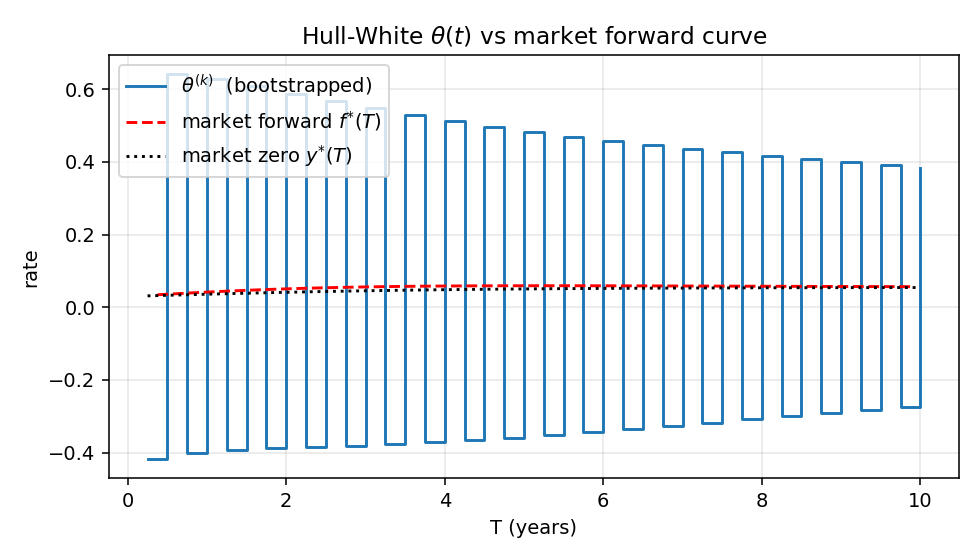
\includegraphics[keepaspectratio]{figures/ch12-theta-vs-fwd.png}}
\emph{\(\theta(t)\) sits slightly above the market forward curve because
of the convexity adjustment \(C_T\).}

\begin{figure}
\centering
\pandocbounded{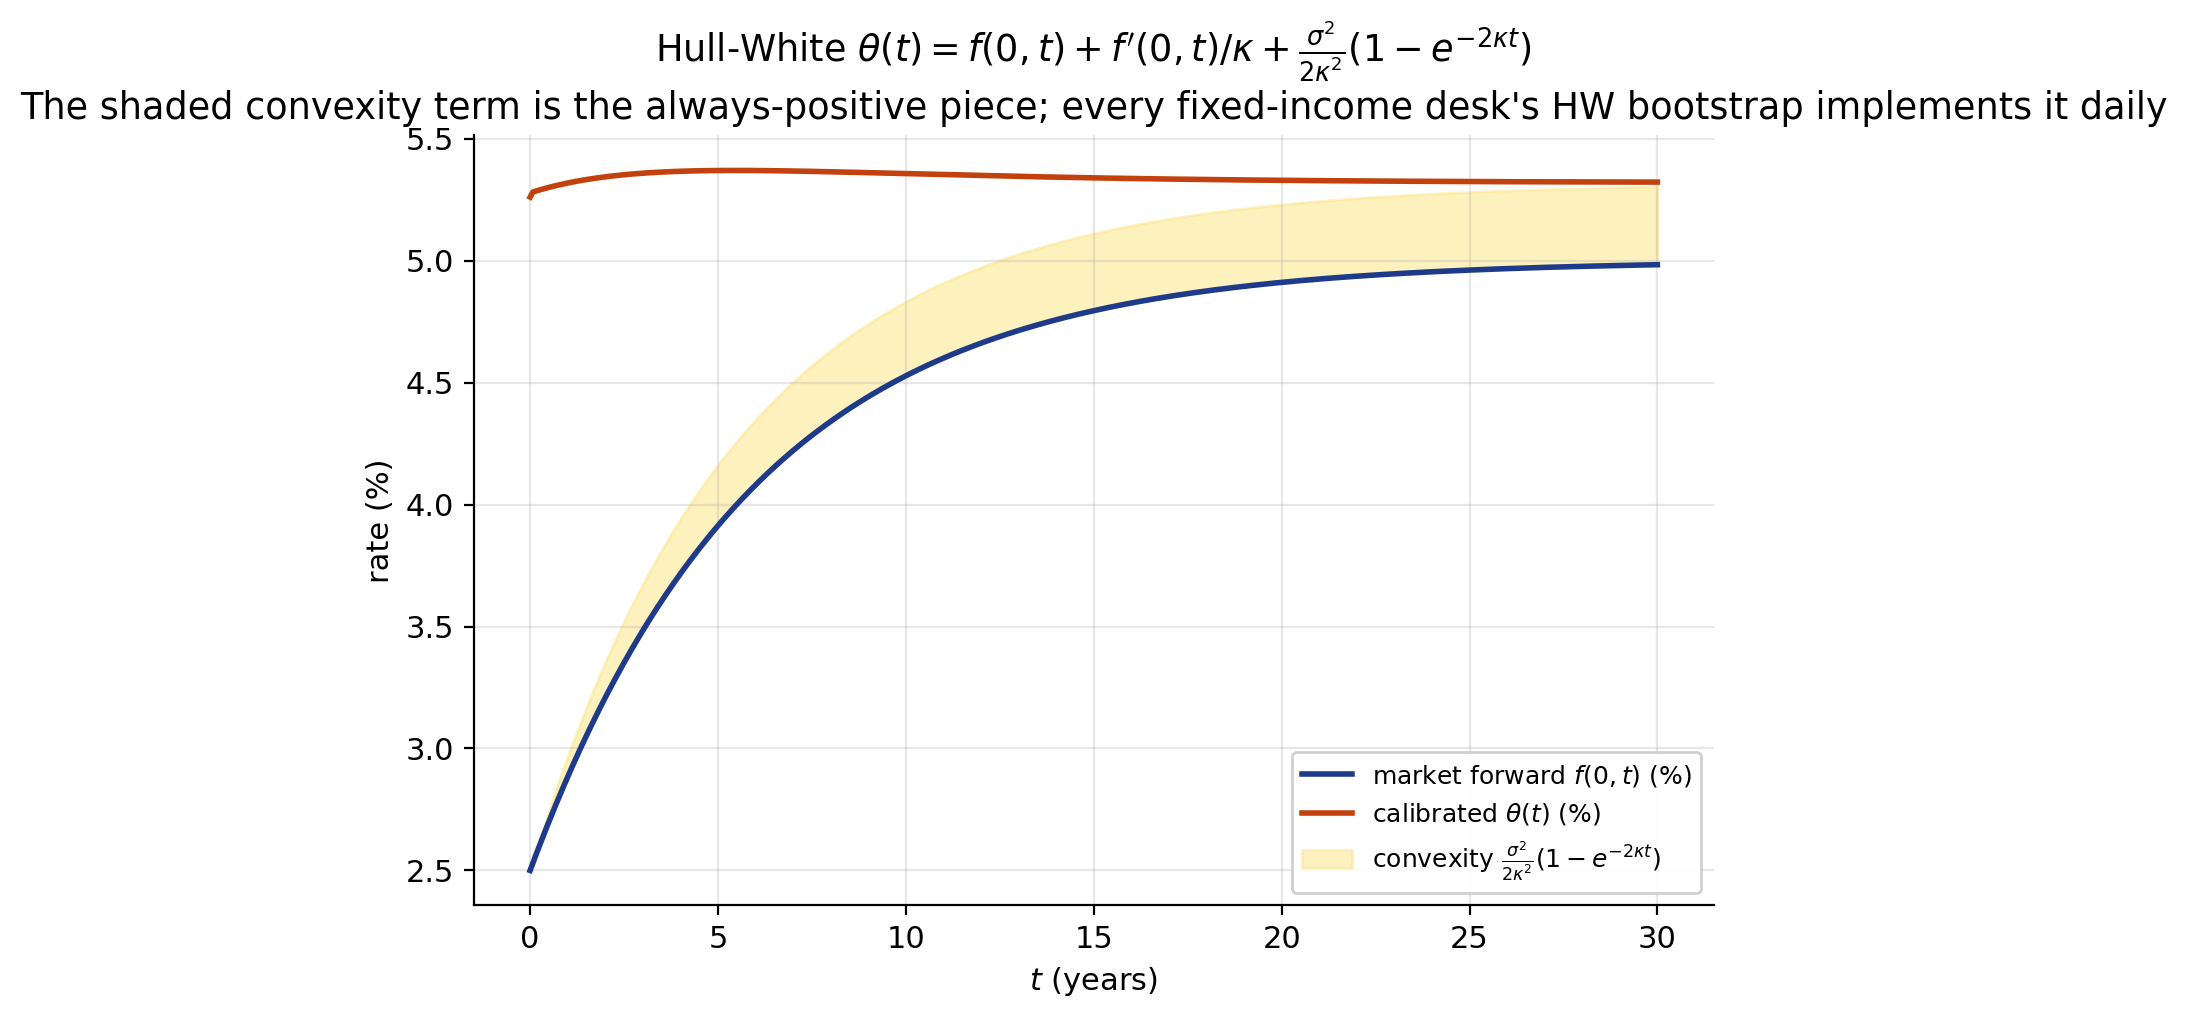
\includegraphics[keepaspectratio]{figures/ch12-hw-theta-fit.png}}
\caption{Hull-White \(\theta(t)\) calibrated to a synthetic market
forward curve, with the convexity gap \(\sim \sigma^2 t/(2\kappa^2)\)
shaded. The same bootstrap runs every morning on every dealer's rates
book --- it's the algorithmic core that converts a swap-curve fit into
an HW-pricer for callables and bermudans}
\end{figure}

For a trader using this model, the practical consequence is that the
calibrated drift schedule \(\theta(t)\) should \emph{not} be interpreted
as ``what the market expects the rate to be at time \(t\).'' That would
only be true in the \(\kappa \to 0\) limit. With mean reversion,
\(\theta(t)\) is instead ``what the target has to be so that the
expected rate path matches the market's forward curve,'' which is
different. The expected rate path itself is
\(\mathbb{E}[r_t] = r_0 e^{-\kappa t} + \kappa\int_0^t
e^{-\kappa(t-u)}\theta_u\,\mathrm{d}u\), which is smoother than
\(\theta(t)\).

\textbf{Philosophical note.} By adjusting \(\theta(t)\) to match today's
curve exactly, Hull-White gives up the possibility of \emph{explaining}
the curve in terms of a small number of stationary parameters. The curve
is now an input, not a prediction. This is a feature for pricing (you
want your model to agree with market quotes) but a bug for economic
insight (you can't test your \(\mathbb{Q}\)-dynamics against curve data
you haven't already used to calibrate them). In this sense Hull-White is
a member of a broad class of ``calibrated'' models in finance whose
primary virtue is practical rather than explanatory.

There is a deeper parallel to the Black-Scholes world. In equity, the
``implied volatility'' surface is what the market uses to quote options;
it is not a model parameter but a derived quantity. In rates, the
forward curve \(f_0(\cdot)\) is what the market quotes; \(\theta(t)\) is
the corresponding derived quantity. Both are ``market-implied'' model
inputs computed from quoted prices via specific formulas.

\subsection{12.6.5 Practical implementation
considerations}\label{practical-implementation-considerations}

The calibration described above is conceptually simple but has several
practical wrinkles worth flagging for someone who will actually
implement it.

\textbf{Curve smoothing.} The pointwise formula (12.52) requires a first
and second derivative of the market forward curve. Real market data
(swap quotes, futures, bond prices) are discrete and noisy; naive
numerical differentiation will produce erratic \(\theta(t)\) that
oscillates between buckets and destabilises the pricing engine.
Production implementations fit a smooth parametric form to the log-
discount curve before differentiating. Common choices include cubic
splines (flexible, but can oscillate near endpoints), Nelson-Siegel
(four parameters capturing level, slope, curvature, and one shape
parameter), Svensson (Nelson-Siegel plus two more parameters for
improved curvature fit), and tension splines (controlled smoothness).
The choice trades off exact fit against parameter stability;
over-smoothed curves produce stale prices, under-smoothed curves produce
noisy prices. The sweet spot is chosen based on the desk's risk appetite
and is re-evaluated periodically.

\textbf{Bucket stability.} Piecewise-constant \(\theta(t)\) has a subtle
defect: the drift is discontinuous at bucket boundaries, producing small
kinks in the implied forward curve. These kinks are usually invisible in
pricing but can show up as spurious ``vol spikes'' in certain risk
metrics. Smoother representations (piecewise linear, cubic splines)
avoid the kinks at the cost of more calibration parameters per bucket. A
compromise is to use piecewise-constant \(\theta(t)\) plus a
post-processing smoothing step that redistributes drift mass across
adjacent buckets while preserving exact bond-price fit. Some
practitioners prefer to parameterise the cumulative integral
\(\Theta(t) = \int_0^t \theta(u)\,\mathrm{d}u\) directly, which is
smoother than \(\theta\) itself.

\textbf{Chicken-and-egg \((\kappa, \sigma, \theta)\) joint calibration.}
The Hull-White convexity term \(C_T\) depends on \((\kappa, \sigma)\),
so bootstrapping \(\theta(t)\) requires knowing these first. But
\((\kappa,
\sigma)\) are typically determined by fitting to caplet and swaption
prices, which themselves depend on the already-extracted \(\theta(t)\).
The standard resolution is iterative: pick initial \((\kappa, \sigma)\)
from historical estimates; extract \(\theta(t)\) via (12.54); fit
\((\kappa, \sigma)\) to option prices; re-extract \(\theta(t)\); iterate
until convergence. In practice convergence is fast (a few iterations)
because the interaction between \(\theta(t)\) and option prices is weak
for typical parameters. Damping, regularisation, and convergence
diagnostics are standard components of serious implementations.

\textbf{Instrument set selection.} Which market instruments should the
model be calibrated to? For vanilla books, the practical answer is: (i)
the short-end of the curve from overnight rates and short-dated futures;
(ii) the intermediate-dated part from medium-term swaps and futures;
(iii) the long end from long-dated swaps; (iv) a strip of ATM caplets or
swaptions for \((\kappa, \sigma)\). For more exotic portfolios (callable
bonds, Bermudan swaptions) additional volatility instruments may be
needed. The calibration error across each instrument set is typically
monitored as a diagnostic; deviations signal either a model limitation
or a data issue.

\textbf{Real-time re-calibration.} Because each calibration step is
linear-time, production systems can re-calibrate every few seconds or
faster as the market ticks. Whether they \emph{should} is a deeper
question: constantly-shifting \(\theta(t)\) muddies P\&L attribution
(``market moved'' vs ``model re-fit'') and creates numerical noise. Most
desks re-calibrate at a few natural cadences (morning open, mid-day, end
of day, plus on large market moves). The choice of cadence is a
trade-off between model freshness and signal-to-noise.

\section{12.7 Affine term structure and the duality of short-rate
models}\label{affine-term-structure-and-the-duality-of-short-rate-models}

The word ``affine'' denotes a very specific class of models with a
precise structural signature: the drift and the squared diffusion of the
state variable are both linear (affine) functions of the state. Vasicek
sits at the simplest end of this class (constant diffusion, linear
drift). CIR complicates matters by allowing the diffusion
\(\sigma\sqrt{r_t}\) to depend on \(r_t\) --- this makes the squared
diffusion \(\sigma^2 r_t\) linear in \(r_t\), so the model is still
affine but the ODE for \(B\) becomes a genuine Riccati equation.
Multi-factor extensions replace \(r_t\) with a vector state and the
scalar ODE for \(B\) with a matrix Riccati ODE. In every case the bond
price remains exponential-affine in the state vector, and that is the
single structural property that makes the entire edifice tractable.

\begin{figure}
\centering
\pandocbounded{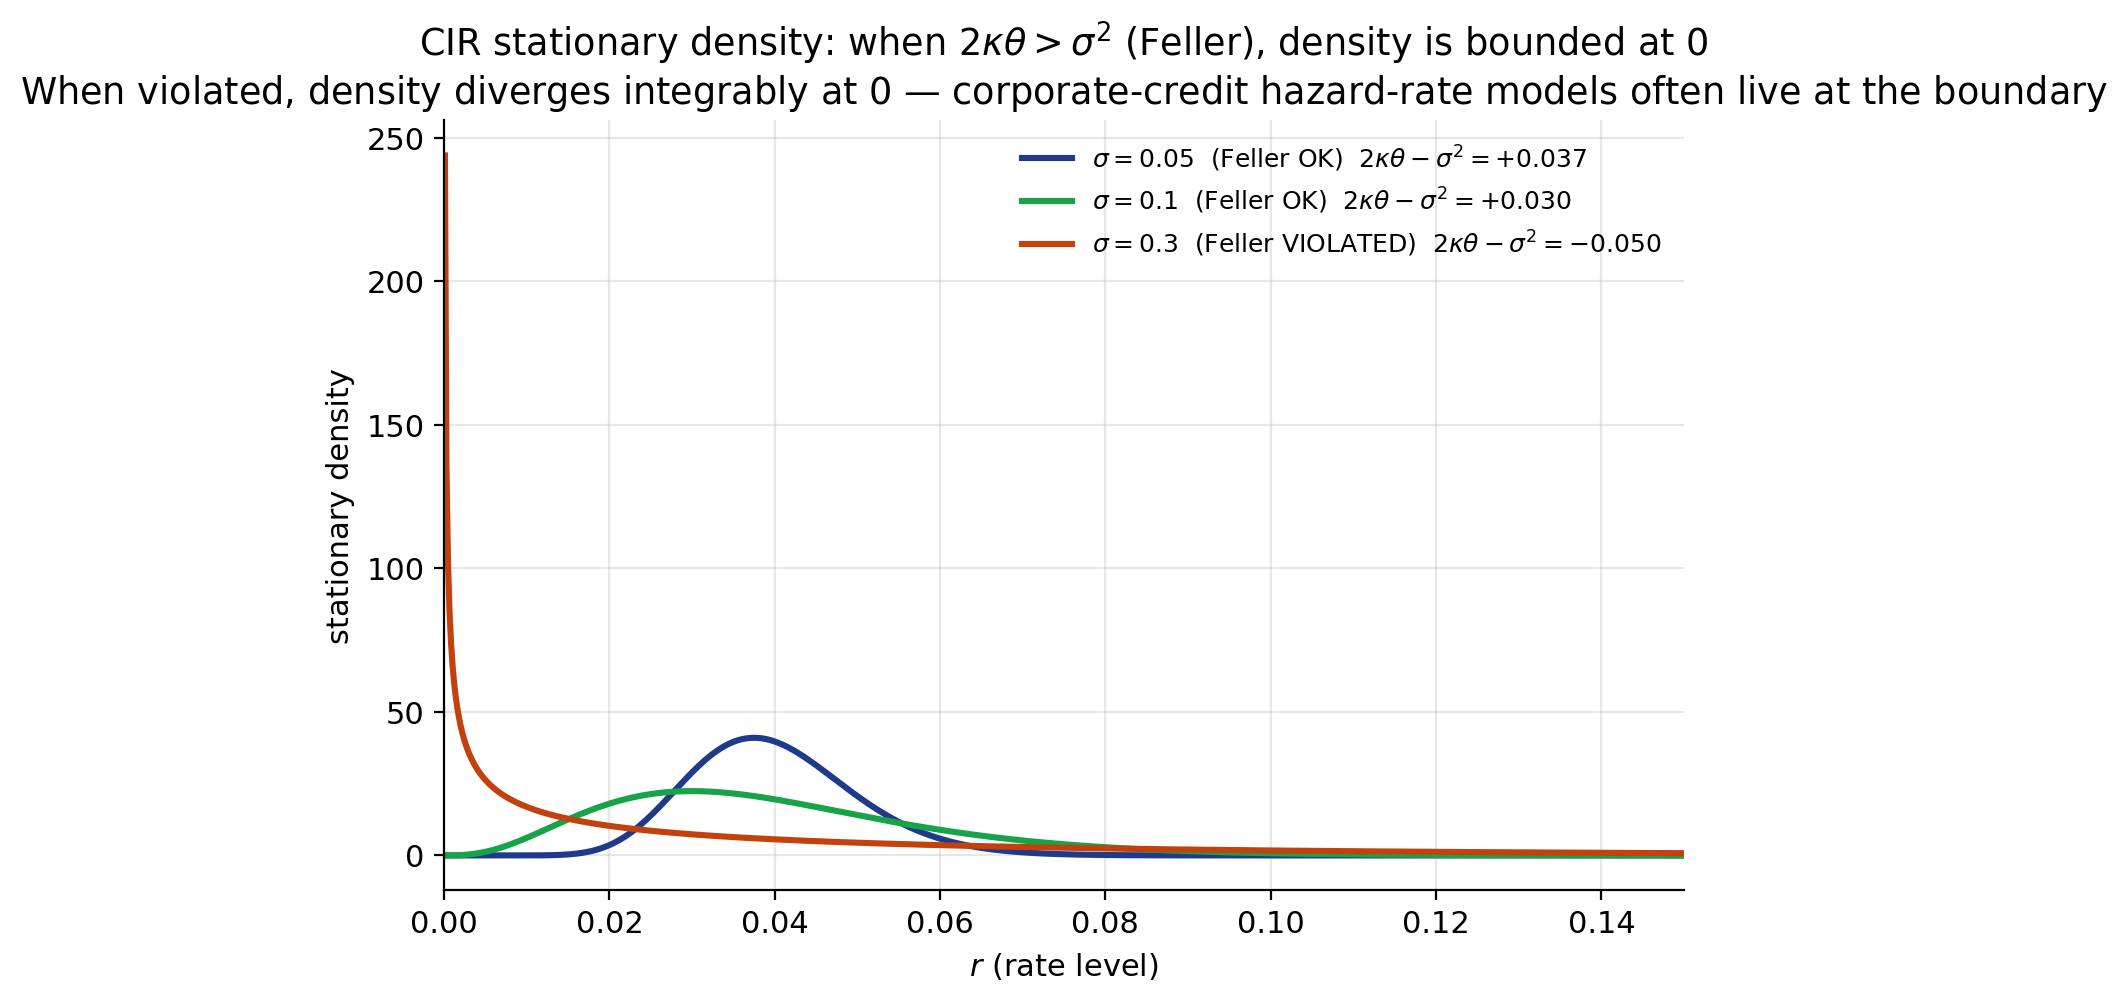
\includegraphics[keepaspectratio]{figures/ch12-cir-zero-boundary.png}}
\caption{CIR stationary density (gamma distributed) under three
\(\sigma\) values: Feller satisfied (bounded at \(r=0\)) vs violated
(divergent but integrable at \(r=0\)). The same boundary controls how
often the variance process in Heston grazes zero --- calibrated SPX
Hestons routinely violate Feller mildly}
\end{figure}

The affine class has been systematically characterised in a celebrated
1996 paper by Duffie and Kan. They showed that if one posits an
exponential-affine bond price \(P(t, T, x) = \exp(A(t, T) + B(t, T)^\top
x)\) for some state vector \(x\), then the underlying state must have a
very restricted form of dynamics: the drift must be affine in \(x\), the
instantaneous covariance matrix must be affine in \(x\) (with
coefficients specifying exactly which linear combinations of state
variables can drive which diagonal entries of the covariance), and the
structure must be compatible across maturities. Moreover, Duffie and Kan
classified the admissible affine models by their ``signature'' ---
whether each state variable can take all real values or must be
non-negative. Vasicek is a pure ``Gaussian'' affine model (all state
variables unconstrained); CIR is a ``square-root'' affine model (one
state variable positive, with \(\sqrt{\cdot}\) diffusion); mixed affine
models combine these. The Duffie-Kan classification underlies
essentially every multi-factor bond-pricing library in practice.

Outside the affine class, exponential-affine bond prices are impossible:
if the dynamics of the state are not affine, the bond price will not
have this form. What do you get instead? Typically, semi-closed-form
approximations (via characteristic functions, transform inversions, or
perturbation expansions), Monte Carlo, or numerical PDE methods. These
techniques work, but they are slower and less transparent than the
affine closed form. For this reason, most practical rates libraries
implement pricing as ``affine-first, with plug-ins for non-affine
corrections.''

\subsection{12.7.1 The three models in one
diagram}\label{the-three-models-in-one-diagram}

The three models derived in this chapter occupy three corners of a small
parameter space:

{\def\LTcaptype{none} % do not increment counter
\begin{longtable}[]{@{}
  >{\raggedright\arraybackslash}p{(\linewidth - 6\tabcolsep) * \real{0.2500}}
  >{\raggedright\arraybackslash}p{(\linewidth - 6\tabcolsep) * \real{0.2500}}
  >{\raggedright\arraybackslash}p{(\linewidth - 6\tabcolsep) * \real{0.2500}}
  >{\raggedright\arraybackslash}p{(\linewidth - 6\tabcolsep) * \real{0.2500}}@{}}
\toprule\noalign{}
\begin{minipage}[b]{\linewidth}\raggedright
Model
\end{minipage} & \begin{minipage}[b]{\linewidth}\raggedright
\(\kappa\)
\end{minipage} & \begin{minipage}[b]{\linewidth}\raggedright
\(\theta\)
\end{minipage} & \begin{minipage}[b]{\linewidth}\raggedright
SDE / bond price
\end{minipage} \\
\midrule\noalign{}
\endhead
\bottomrule\noalign{}
\endlastfoot
Ho-Lee & \(0\) & \(\theta(t)\) &
\(\mathrm{d}r_t = \theta(t)\,\mathrm{d}t + \sigma\,\mathrm{d}W_t\);
\(\ln P_0(T)\) has \(+\sigma^2 T^3/6\) convexity \\
Vasicek & \(\kappa > 0\) & constant &
\(\mathrm{d}r_t = \kappa(\theta - r_t)\,\mathrm{d}t + \sigma\,\mathrm{d}W_t\);
\(P_t(T) = e^{A_t(T) - B_t(T)r_t}\) affine \\
Hull-White & \(\kappa > 0\) & \(\theta(t)\) & Vasicek dynamics with
\(\theta_t\) calibrated to market curve \\
\end{longtable}
}

The nesting is transparent: Hull-White \(\supset\) Vasicek \(\supset\)
Ho-Lee, with each inclusion obtained by freezing one more parameter.
Vasicek is Hull-White with \(\theta_t\) held constant; Ho-Lee is
Hull-White with \(\kappa \to 0\) (and the \(\kappa\theta_t\) product
held fixed). In production use, Hull-White is almost always the model of
choice because it is the only one of the three that fits the observed
yield curve exactly.

\subsection{12.7.2 Duality: three perspectives on the same
formula}\label{duality-three-perspectives-on-the-same-formula}

The bond price \(P_t(T) = e^{A_t(T) - B_t(T)r_t}\) can be derived by
three independent routes, each shining light on a different aspect:

\begin{enumerate}
\def\labelenumi{\arabic{enumi}.}
\tightlist
\item
  \textbf{Direct expectation (§12.3.4, §12.5.3, §12.6.3).} Use the
  explicit Gaussian solution for \(r_t\), integrate to get the Gaussian
  law of \(\int_t^T r_u\,\mathrm{d}u\), apply the moment-generating
  function. This route makes the Jensen-convexity origin of the formula
  transparent and generalises to any Gaussian affine model.
\item
  \textbf{Affine ansatz + PDE (§12.3.5).} Use Feynman-Kac to convert the
  expectation into a parabolic PDE with source term \(-rg\); guess an
  exponential-affine solution; match coefficients to obtain a pair of
  ODEs for \(A\) and \(B\). This route makes the affine structure of the
  model explicit and generalises to any affine model including CIR and
  quadratic-Gaussian.
\item
  \textbf{Martingale verification (discussed but not executed).}
  Postulate the formula \(P = e^{A - Br}\), compute \(\mathrm{d}(P/M)\)
  using Itô, verify that the drift is zero under \(\mathbb{Q}\). This
  route directly confirms the no-arbitrage condition and is the most
  elegant but requires pre-knowledge of the formula.
\end{enumerate}

That all three converge on the same answer is both a consistency check
and a window onto the structural richness of affine models. Each route
carries some information the others don't: the direct expectation
carries the probabilistic intuition (Jensen, Gaussian MGF); the PDE
carries the analytic intuition (elliptic operators, Riccati ODEs); the
martingale verification carries the economic intuition (no-arbitrage as
martingality). Mastering all three is the difference between pricing a
bond and understanding what its price means.

\subsection{12.7.3 Where this chapter leaves the
reader}\label{where-this-chapter-leaves-the-reader}

By the end of §12.6 the reader can:

\begin{itemize}
\tightlist
\item
  Derive Vasicek from first principles, arriving at the bond-price
  formula (12.20)-(12.22) by both the direct-expectation and PDE routes.
\item
  Extend to Hull-White by letting \(\theta \to \theta(t)\), and
  bootstrap \(\theta(t)\) to exactly reproduce an observed yield curve.
\item
  Specialise to Ho-Lee by setting \(\kappa \to 0\), with the
  understanding that the resulting cubic variance growth limits the
  model to short-dated products.
\item
  Read off the yield curve, forward curve, and convexity adjustment as
  analytical by-products.
\end{itemize}

What is \emph{not} in this chapter: applications. The IRS par-rate
formula, the Jamshidian bond-option formula, the T-forward measure,
callable bonds, CDS, and multi-factor / LMM / SABR all live in Chapter
13 (rate derivatives) and Chapter 14 (caps and swaptions). The division
of labour is: this chapter \emph{builds the model}; the next two
\emph{use it}.

\begin{center}\rule{0.5\linewidth}{0.5pt}\end{center}

\subsection{Case study (a): Negative Eurozone rates 2014--2022 ---
Vasicek vs
CIR}\label{case-study-a-negative-eurozone-rates-20142022-vasicek-vs-cir}

\emph{The ECB cut its deposit facility rate to \(-0.10\%\) on 5 June
2014 --- the first time a major central bank had taken a policy rate
negative --- and held it negative through to 27 July 2022, hitting
\(-0.50\%\) in September 2019. Swiss and Danish policy rates went
deeper; the 10-year Bund traded at \(-0.74\%\) in March 2020. For an
entire decade EUR rates desks priced and hedged in a regime that one
canonical short-rate model (CIR) literally cannot represent and another
(Vasicek / Hull-White) handles unchanged.}

\textbf{Context.} The Cox-Ingersoll-Ross (1985) model
\(\mathrm{d}r_t = \kappa(\theta - r_t)\,\mathrm{d}t + \sigma\sqrt{r_t}\,\mathrm{d}W_t\)
was historically attractive for two reasons: its Feller-square-root
diffusion produces a non-central chi-squared distribution for \(r_T\)
supported on \([0, \infty)\), ruling out negative rates ``for free'',
and its bond price is affine and closed-form. Both features were sold as
virtues for decades. Vasicek's
\(\mathrm{d}r_t = \kappa(\theta - r_t)\,\mathrm{d}t + \sigma\,\mathrm{d}W_t\),
by contrast, is Gaussian --- \(r_T\) is normal on all of \(\mathbb{R}\),
and a fraction of probability mass always sits below zero. Pre-2014
textbooks routinely flagged this as a Vasicek ``defect'' and recommended
CIR for production rate-modelling work. Hull-White, the
time-inhomogeneous Gaussian extension, inherits the same
support-on-\(\mathbb{R}\) property and the same alleged ``defect.''

When EONIA dropped below zero in mid-2014, every CIR-based EUR rates
book had a problem the model literally could not articulate. A 5y
receiver swaption struck at \(-0.25\%\) has positive intrinsic value
when forward rates trade at \(-0.40\%\), but CIR cannot generate sample
paths reaching \(-0.25\%\) at all --- its short-rate density is
identically zero on \((-\infty, 0)\). Banks responded with three
workarounds, all bad: (i) shift the rate process, \(r_t = x_t - s\) with
\(x_t\) CIR and \(s = 1\%\) a fixed shift, recovering negative-rate
support but contaminating mean-reversion estimates; (ii) re-derive
prices in a ``shadow rate'' framework where the observed rate is
\(r_t = \max(x_t - s, -\bar r)\), breaking closed-form pricing; (iii)
abandon CIR for Hull-White (Gaussian, time-inhomogeneous), eat the
migration cost across the entire book, and live with negative-rate-tail
probabilities that some risk committees still found uncomfortable. The
third option won at every major EUR rates desk during 2014-2017.

\textbf{Reading it through the chapter's math.} Vasicek's explicit
solution (12.12) and the law of \(r_T\) in §12.3.2 are unconditionally
Gaussian: \(r_T \sim \mathcal{N}(\mathbb{E}[r_T], \mathbb{V}[r_T])\) on
all of \(\mathbb{R}\), regardless of the sign of \(\theta\) or the value
of \(r_0\). The Vasicek closed-form bond price (12.20) is
\(A(t,T)\exp(-B(t,T) r_t)\) with \(B > 0\), so as \(r_t \to -\infty\)
the bond price goes to \(+\infty\) --- there is no degeneracy at zero.
CIR's affine form has the same superficial structure but the underlying
distributional law is non-central chi-squared with a degree-of-freedom
parameter that determines whether zero is an attainable, repelling, or
absorbing boundary; either way, the support is \([0, \infty)\) by
construction. Pricing a \(-0.25\%\)-strike receiver swaption in CIR is
mathematically a request for \(\mathbb{E}^{\mathbb{Q}}[(K - L_T)^+]\)
with \(K = -0.25\%\) and \(L_T \ge 0\); the answer is \(|K|\) times the
annuity, i.e.~the swaption is automatically maximally in-the-money for
any negative strike, which is wrong by construction (the actual EUR
fixings did move further negative, so the receiver was \emph{not}
maximally ITM). The two models gave genuinely different prices for
receiver swaptions near the zero bound --- sometimes \(5\%\)--\(10\%\)
of premium --- and the Vasicek/Hull-White price was the correct one in
every case.

\textbf{Lesson.} A model's state space is not a regularisation choice;
it is a structural assertion about what realities the model can
describe. CIR went out of fashion in EUR rates for the better part of a
decade not because it was poorly calibrated, but because the rates desks
woke up one morning in June 2014 in a regime CIR's ontology forbade. The
Hull-White migration cost --- re-implementation, re-validation,
re-calibration of every Bermudan and callable structure on the book ---
was substantial; banks that delayed paid for it in mispriced
negative-rate exotics for years. The deeper lesson for the new hire:
when choosing a short-rate model for a given currency, the support of
the rate distribution is the first question to ask, ahead of
mean-reversion realism, ahead of analytic tractability, ahead of
computational cost. Models with non-negative-rate hard floors (CIR, BK,
square-root Hull-White) belong only in regimes where the central bank's
reaction function genuinely rules out negative rates as policy ---
historically, USD before 2008 and emerging markets. Anywhere else, the
Gaussian family (Vasicek, Hull-White, G2++) is the safe default, and the
negative-rate tail probability that risk committees worry about is in
fact a \emph{feature}, not a bug.

\begin{center}\rule{0.5\linewidth}{0.5pt}\end{center}

\subsection{\texorpdfstring{Case study (b): 2023 Fed hiking cycle ---
Hull-White \(\theta(t)\) bootstrap from the funds
curve}{Case study (b): 2023 Fed hiking cycle --- Hull-White \textbackslash theta(t) bootstrap from the funds curve}}\label{case-study-b-2023-fed-hiking-cycle-hull-white-thetat-bootstrap-from-the-funds-curve}

\emph{Between March 2022 and July 2023 the Fed funds target rose from
\(0.00\)--\(0.25\%\) to \(5.25\)--\(5.50\%\) in eleven hikes --- the
fastest hiking cycle since Volcker. By the second half of 2023 the curve
was deeply inverted: \(3\)M \(\approx 5.45\%\), \(4\)M
\(\approx 5.40\%\), \(2\)Y \(\approx 4.85\%\), \(5\)Y
\(\approx 4.40\%\), \(10\)Y \(\approx 4.25\%\). Pricing a \(\$50\)B
Bermudan callable book against this curve, every single morning, is what
Hull-White's \(\theta(t)\) bootstrap was designed for.}

\textbf{Context.} Hull-White's defining feature, relative to
constant-coefficient Vasicek, is the time-dependent drift \(\theta(t)\)
chosen so that the model's initial discount curve
\(P_0^{\mathrm{HW}}(0, T)\) matches today's market discount curve
\(P_0^{\mathrm{mkt}}(0, T)\) for every \(T\). The calibration identity
in §12.6.4 --- solve for \(\theta(t)\) such that the Hull-White bond
formula reproduces every market zero --- is \emph{linear} in
\(\theta(t)\) once \((\kappa, \sigma)\) are fixed, and runs in
\(\mathcal{O}(\text{tenors})\) per re-calibration. In 2023 with
\(\kappa = 0.06\) (calibrated from swaption-vol smile slope) and
\(\sigma = 0.011\) (calibrated from caplet ATM vols), the entire
\(\theta(t)\) bootstrap across \(40\) tenor buckets ran in under \(5\)
ms on a single core. Every \(8{:}00\) AM the curve desk would lift the
overnight Treasury and OIS quotes, build the discount curve, and refresh
\(\theta(t)\) --- the whole process from market data to Bermudan
repricing was sub-second.

The calibration mechanic for an inverted curve is genuinely informative
about the underlying risk picture, in a way the constant-\(\theta\)
Vasicek calibration is not. With a flat curve, \(\theta(t)\) comes out
roughly flat at the long-run mean \(\theta_\infty\) and the calibration
carries little information beyond what the AR(1) coefficient already
encoded. With the steeply inverted 2H 2023 curve, \(\theta(t)\) took a
distinctive shape: \(\theta(0\)--\(1y) \approx 5.4\%\), peaking just
above the spot rate (the model needs a slightly higher mean-reversion
target to keep the front rates from collapsing immediately), then
declining smoothly to \(\theta(5y) \approx 3.8\%\) and
\(\theta(10y) \approx 3.3\%\). The convexity adjustment
\(C_T = \tfrac{1}{2}\sigma^2 B(t,T)^2\) in (12.51) added \(+2\)--\(4\)
bp lift at each maturity bucket, which the desk treated as a separate
Greek for hedging --- that adjustment is entirely a function of
\(\sigma\), and it is the reason why a higher real-rate vol
\emph{raises} model-implied long forwards above what the spot curve
alone would indicate.

\textbf{Reading it through the chapter's math.} The bootstrap proceeds
tenor-by-tenor (§12.6.4 procedure): given the calibrated
\((\kappa, \sigma)\), the Hull-White zero-coupon price is
\(P^{\mathrm{HW}}(0, T) = \exp(-\int_0^T f^{\mathrm{HW}}(0, u)\,\mathrm{d}u)\)
with \(f^{\mathrm{HW}}(0, u)\) a closed-form linear functional of
\(\theta(\cdot)\) on \([0, u]\). Inverting,
\(\theta(u) = \partial_u f^{\mathrm{mkt}}(0, u) + \kappa f^{\mathrm{mkt}}(0, u) + \tfrac{\sigma^2}{2\kappa}(1 - e^{-2\kappa u})\)
--- the famous Hull-White \(\theta\)-formula, where the first two terms
recover the market forward and its slope, and the third is the convexity
correction that depends only on \(\sigma\). The inverted 2023 curve has
\(\partial_u f^{\mathrm{mkt}}(0, u) < 0\) for \(u > 1\)y, so the
\(\theta(u)\) schedule slopes downward through the belly. But the
convexity term is \emph{always positive} and grows with \(\sigma\): a
higher real-rate vol pushes \(\theta(u)\) upward at every maturity, and
the model's forward curve up by approximately
\(\tfrac{1}{2}\sigma^2 B(0, u)^2\) above the spot forward. In late 2023,
with realised real-rate vol around \(\sigma = 1.1\%\), the convexity
adjustment at \(10\)y was \(\approx 18\) bp --- non-trivial relative to
the inversion gap. The inversion \emph{plus} the high vol therefore
meant: market expects cuts (declining \(\theta\) through belly), but the
cuts are uncertain enough in timing that convexity adds a meaningful
upward push to long-end model forwards.

\textbf{Lesson.} Hull-White's exact-fit-to-curve property is not
optional infrastructure during a regime shift like the 2023 hiking cycle
--- it is what lets a desk hedge a multi-tens-of-billions Bermudan book
against a moving Fed without generating spurious model-misfit P\&L. A
constant-\(\theta\) Vasicek would have left a \(50\)+ bp residual at the
front of the curve, contaminating every \(\Delta\)-vega report on the
book; the Bermudan call decisions (whether to call at the next exercise
date) would be driven as much by model error as by genuine moneyness.
The deeper lesson for the new hire is to read the \emph{shape} of the
calibrated \(\theta(t)\) schedule as a market signal rather than as a
fitted nuisance: a downward-sloping \(\theta(t)\) is the market telling
you cuts are priced; the magnitude of the convexity adjustment is the
market telling you how \emph{uncertain} those cuts are; the day-to-day
stability of \(\sigma\) tells you whether realised vol has caught up to
implied. None of these pieces is what Hull-White was originally designed
to communicate, but in a fast-moving rate cycle they become the most
useful operational diagnostics on the desk.

\begin{center}\rule{0.5\linewidth}{0.5pt}\end{center}

\section{12.8 Key Takeaways}\label{key-takeaways-11}

\begin{enumerate}
\def\labelenumi{\arabic{enumi}.}
\item
  \textbf{Short rates are not traded; bonds are.} The Fundamental
  Theorem of Asset Pricing applies to tradables, so the risk-neutral
  measure \(\mathbb{Q}\) is defined by its action on \(M_t\) and
  \(P_t(T)\), not on \(r_t\). This creates a genuine degree of freedom
  (the market price of risk \(\lambda_t\)) that must be fixed externally
  --- typically by calibration to observed bond prices.
\item
  \textbf{The master pricing formula is
  \(P_t(T) = \mathbb{E}^{\mathbb{Q}}_t[e^{-\int_t^T r_s\,\mathrm{d}s}]\).}
  It is model-agnostic --- every short-rate model computes the same
  conditional expectation, differing only in how the expectation is
  evaluated. Affine models evaluate it in closed form.
\item
  \textbf{Vasicek: three parameters, one bond-price formula.} The SDE
  \(\mathrm{d}r_t = \kappa(\theta - r_t)\,\mathrm{d}t +
  \sigma\,\mathrm{d}W_t\) yields, via either the direct-expectation
  route or the PDE / affine-ansatz route, the closed-form bond price
  \(P_t(T) = e^{A_t(T) - B_t(T) r_t}\) with \(B_t(T) = (1 -
  e^{-\kappa(T-t)})/\kappa\).
\item
  \textbf{Bonds are convex in rates (Jensen's mountain).} The
  \(+\tfrac{1}{2}\Sigma_*^2\) term in the Gaussian MGF is the convexity
  adjustment that makes long bonds worth \emph{more} than naive plug-in
  discounting suggests. It explains why long yields trade below expected
  long-run short rates even without a term premium.
\item
  \textbf{Long-bond duration is capped at \(1/\kappa\).} This is
  Vasicek's most economically distinctive prediction: unlike a
  random-walk rate model, mean reversion means long bonds have finite
  sensitivity to the current short rate. Any calibrated \(\kappa\)
  outside the range \([0.1, 0.5]\) is suspect.
\item
  \textbf{Long yield = \(\theta - \tfrac{1}{2}\sigma^2/\kappa^2\).} The
  long end of the yield curve is \emph{below} the long-run mean of the
  short rate by a convexity premium. Larger in high-vol or
  slow-reverting regimes.
\item
  \textbf{Ho-Lee is the \(\kappa \to 0\) limit.} Pure random walk with
  time-varying drift. Bond price has the simple form
  \(\ln P_0(T) = -r_0 T - \iint\theta + \sigma^2 T^3/6\); drift
  pointwise calibration
  \(\theta_T = -\partial_T^2 \ln P_0^*(T) + \sigma^2 T\). The cubic
  \(T^3\) variance growth means Ho-Lee breaks at long maturities.
\item
  \textbf{Hull-White = Vasicek with time-varying \(\theta(t)\).} Exact
  yield-curve fit by construction, via a linear triangular bootstrap
  (12.54) analogous to Ho-Lee's. Two-stage calibration in practice:
  \((\kappa, \sigma)\) fit to swaption vols, then \(\theta(t)\)
  bootstrapped to match bonds.
\item
  \textbf{One-factor is a limitation.} Vasicek/HW can only produce
  parallel-shift curve moves (up to the \(B_t(T)\) loading). Real curve
  dynamics have three factors (level, slope, curvature); for hedging and
  pricing curve-twist-sensitive products, move to G2++ or multi-factor
  affine or LMM.
\item
  \textbf{Affine = tractable.} The structural property ``drift linear,
  squared diffusion linear in the state'' is what makes coefficient-
  matching work in the PDE ansatz, reduces the infinite-dimensional
  pricing problem to two ODEs, and ultimately gives closed-form bond
  prices. Ho-Lee, Vasicek, HW, CIR, G2++, and the Duffie-Kan affine
  family all share this property; Black-Karasinski (log-rate) and
  stochastic-vol rates models do not.
\end{enumerate}

\begin{center}\rule{0.5\linewidth}{0.5pt}\end{center}

\section{12.9 Reference Formulas}\label{reference-formulas-7}

\subsection{Core dynamics}\label{core-dynamics}

\[
\mathrm{d}r_t = \kappa(\theta(t) - r_t)\,\mathrm{d}t + \sigma\,\mathrm{d}\widehat{W}_t
\]

\begin{itemize}
\tightlist
\item
  \$\theta(t) = \$ const gives Vasicek; \(\kappa = 0\) gives Ho-Lee.
\end{itemize}

\subsection{Explicit solution}\label{explicit-solution}

\[
r_T = e^{-\kappa(T-t)}\, r_t + \kappa\!\int_t^T e^{-\kappa(T-s)}\theta(s)\,\mathrm{d}s + \sigma\!\int_t^T e^{-\kappa(T-s)}\,\mathrm{d}\widehat{W}_s
\]

\subsection{\texorpdfstring{Distribution of \(r_T\) (Vasicek, const
\(\theta\))}{Distribution of r\_T (Vasicek, const \textbackslash theta)}}\label{distribution-of-r_t-vasicek-const-theta}

\[
r_T \;\sim\; \mathcal{N}\!\left(\theta + e^{-\kappa(T-t)}(r_t - \theta),\;\; \tfrac{\sigma^2}{2\kappa}\bigl(1 - e^{-2\kappa(T-t)}\bigr)\right)
\]

Stationary limit: \(\mathcal{N}(\theta, \sigma^2/(2\kappa))\).

\subsection{Integrated rate (Vasicek)}\label{integrated-rate-vasicek}

\[
\int_t^T r_s\,\mathrm{d}s \;=\; B_t(T)\, r_t + \theta\bigl((T-t) - B_t(T)\bigr) + \tfrac{\sigma}{\kappa}\!\int_t^T\bigl(1 - e^{-\kappa(T-s)}\bigr)\,\mathrm{d}\widehat{W}_s
\]

Gaussian with mean and variance in (12.16)-(12.18).

\subsection{Vasicek affine bond price}\label{vasicek-affine-bond-price}

\[
P_t(T) = e^{A_t(T) - B_t(T)\, r_t}, \qquad B_t(T) = \frac{1 - e^{-\kappa(T-t)}}{\kappa}
\]

\[
A_t(T) = -\theta\bigl((T-t) - B_t(T)\bigr) + \tfrac{\sigma^2}{2\kappa^2}\!\int_t^T\bigl(1 - e^{-\kappa(T-s)}\bigr)^2\,\mathrm{d}s
\]

\subsection{Affine ansatz ODE system}\label{affine-ansatz-ode-system}

\[
\begin{cases}
\dot{A}_t - \kappa B_t\, \theta(t) + \tfrac{1}{2}\sigma^2 B_t^2 = 0 \\[3pt]
\dot{B}_t - \kappa B_t + 1 = 0
\end{cases}
\qquad A_T = B_T = 0
\]

\subsection{Vasicek yield curve}\label{vasicek-yield-curve}

\[
y_t(T) = \frac{B_t(T)\,r_t - A_t(T)}{T - t}
\]

Limits: \(y_t(t) = r_t\);
\(y_t(\infty) = \theta - \tfrac{1}{2}\sigma^2/\kappa^2\).

\subsection{Ho-Lee bond price}\label{ho-lee-bond-price}

\[
\ln P_0(T) \;=\; -r_0\,T \;-\; \int_0^T\!\int_0^u \theta_s\,\mathrm{d}s\,\mathrm{d}u \;+\; \frac{\sigma^2 T^3}{6}
\]

\subsection{Ho-Lee calibration
identity}\label{ho-lee-calibration-identity}

\[
\theta_T \;=\; -\,\partial_T^2 \ln P_0^*(T) \;+\; \sigma^2 T \;=\; \partial_T f_0(T) + \sigma^2 T
\]

\subsection{Hull-White bond price}\label{hull-white-bond-price-1}

\[
P_0(T) = \exp\{-r_0\,B_T - A_T + C_T\}
\]

\[
B_T = \frac{1 - e^{-\kappa T}}{\kappa}, \quad A_T = \int_0^T \theta_u\bigl(1 - e^{-\kappa(T-u)}\bigr)\,\mathrm{d}u, \quad C_T = \frac{\sigma^2}{2\kappa^2}\int_0^T\!\bigl(1 - e^{-\kappa(T-u)}\bigr)^2\,\mathrm{d}u
\]

\subsection{Hull-White pointwise
calibration}\label{hull-white-pointwise-calibration}

\[
\theta(T) \;=\; \frac{1}{\kappa}\,\partial_T f_0(T) + f_0(T) + \frac{\sigma^2}{2\kappa^2}\bigl(1 - e^{-2\kappa T}\bigr)
\]

\subsection{Hull-White bucket
bootstrap}\label{hull-white-bucket-bootstrap}

\[
\theta^{(k)} \;=\; \frac{T_k\,y_k^* - r_0\,B_{T_k} + C_{T_k} - \sum_{m=1}^{k-1}\theta^{(m)}\,\alpha^{(m,k)}}{\alpha^{(k,k)}}
\]

with

\[
\alpha^{(m,k)} \;=\; (T_m - T_{m-1}) \;-\; \frac{e^{-\kappa(T_k - T_m)} - e^{-\kappa(T_k - T_{m-1})}}{\kappa}.
\]

\subsection{Three-model nesting}\label{three-model-nesting}

{\def\LTcaptype{none} % do not increment counter
\begin{longtable}[]{@{}
  >{\raggedright\arraybackslash}p{(\linewidth - 8\tabcolsep) * \real{0.2000}}
  >{\raggedright\arraybackslash}p{(\linewidth - 8\tabcolsep) * \real{0.2000}}
  >{\raggedright\arraybackslash}p{(\linewidth - 8\tabcolsep) * \real{0.2000}}
  >{\raggedright\arraybackslash}p{(\linewidth - 8\tabcolsep) * \real{0.2000}}
  >{\raggedright\arraybackslash}p{(\linewidth - 8\tabcolsep) * \real{0.2000}}@{}}
\toprule\noalign{}
\begin{minipage}[b]{\linewidth}\raggedright
Model
\end{minipage} & \begin{minipage}[b]{\linewidth}\raggedright
\(\kappa\)
\end{minipage} & \begin{minipage}[b]{\linewidth}\raggedright
\(\theta\)
\end{minipage} & \begin{minipage}[b]{\linewidth}\raggedright
Long-run \(\mathbb{V}[r_T]\)
\end{minipage} & \begin{minipage}[b]{\linewidth}\raggedright
Convexity \(C_T\) as \(T\to\infty\)
\end{minipage} \\
\midrule\noalign{}
\endhead
\bottomrule\noalign{}
\endlastfoot
Ho-Lee & \(0\) & \(\theta(t)\) & \(\sigma^2 T\) & \(\sigma^2 T^3/6\)
(cubic) \\
Vasicek & \(\kappa > 0\) & const & \(\sigma^2/(2\kappa)\) & linear
growth (\(\sim \sigma^2/(2\kappa^2)\cdot(T-t)\) asymptotically) \\
Hull-White & \(\kappa > 0\) & \(\theta(t)\) & \(\sigma^2/(2\kappa)\) &
\(\sigma^2 T/(2\kappa^2)\) (linear) \\
\end{longtable}
}

\subsection{Half-life}\label{half-life}

\[
\tau_{1/2} = \frac{\ln 2}{\kappa}
\]

Typical calibrated \(\kappa \in [0.1, 0.5]\) corresponds to rate-shock
half-lives of 1.4 to 7 years.

\newpage

\chapter{Chapter 13 --- Rate-Derivative Applications: Swaps, CDS, Bond
Options,
Callables}\label{chapter-13-rate-derivative-applications-swaps-cds-bond-options-callables}

\section{13.1 From short-rate dynamics to products that depend on
them}\label{from-short-rate-dynamics-to-products-that-depend-on-them}

Chapter 12 built the Vasicek, Ho-Lee, and Hull-White short-rate models
--- the SDEs, the integrated-rate distributions, the closed-form bond
prices, the affine-ODE system, the calibration of \(\theta_t\) to
today's curve. All of that machinery was developed with one pay-off in
mind: \emph{use it to price rate-dependent products}. This chapter is
that pay-off. We take the calibrated short-rate model from Chapter 12 as
given and work outward to the four product classes that dominate rates
desks: \textbf{interest-rate swaps (IRS)}, \textbf{callable bonds},
\textbf{credit default swaps (CDS)}, and \textbf{European bond options}
(together with their capstone application, swaptions via the Jamshidian
decomposition). We close with a tour of where the single-factor Gaussian
framework starts to break and which extensions (HJM, LMM, SABR,
multi-factor Gaussian) handle the residual.

The chapter is organised by how much of the short-rate model each
product actually uses. Swaps are almost model-free: only the discount
curve enters, so Vasicek versus Hull-White versus any other
calibrated-curve model gives the same swap value. Callable bonds are
genuinely model-dependent: the embedded American option on a bond
requires a backward induction on a short-rate tree, and both the level
of rates and the variance of the short rate matter. CDS depend on the
calibrated discount curve plus a separate hazard-rate curve; the two
combine into a risky discount factor. European bond options under
Vasicek/Hull-White admit a clean closed-form (the Jamshidian /
Vasicek-Black formula), and the derivation is the canonical application
of the \textbf{T-forward measure} --- a specific change of numeraire
that makes the forward bond price a martingale with deterministic
volatility. Crucially, we will \emph{not} re-derive Girsanov's theorem
or the T-forward measure here: Chapter 5 already did that once. This
chapter cites the result from Chapter 5 and uses it.

\textbf{A roadmap to the rest of the chapter.} §13.2 prices an IRS and
extracts the par swap rate --- a model-free calculation that exercises
only the discount curve. §13.3 tackles callable bonds on a Hull-White
trinomial tree, introducing the backward-induction-plus-early-exercise
pattern that appears again and again in rate-derivative pricing. §13.4
handles CDS with constant and time-varying hazard, deriving the ``credit
triangle'' \(S \approx (1-R)\lambda\) and its corrections. §13.5 takes a
visual pause on the yield surface --- a 3D object that is the natural
state of the rates-trading book. §13.6 derives the Vasicek-Black
bond-option formula via the T-forward measure, citing Chapter 5 for the
Girsanov apparatus. §13.7 walks through worked examples of that formula
and introduces the Jamshidian decomposition that reduces a swaption to a
portfolio of bond options. §13.8 previews where we go beyond
single-factor Vasicek: the multi-factor Gaussian G2++, HJM, LMM, and
SABR. §13.9 closes with the PDE-versus-Monte-Carlo trade-offs that
dictate which numerical method a rates desk deploys per product. §13.10
summarises the chapter; §13.11 is the reference-formula appendix.

The conceptual thread running through all five products is this:
\textbf{every rate derivative is a functional of the future yield curve,
and pricing it reduces to computing a conditional expectation of that
functional under some convenient martingale measure}. The specific
measure depends on when the payoff settles and what numeraire most
naturally absorbs its stochastic discount factor. For swaps we use no
measure machinery at all --- the linearity-in-rates of the payoff lets
us replicate and price pathwise. For CDS we use \(\mathbb{Q}\) with a
hazard-rate extension. For bond options we use the T-forward measure.
For swaptions we use the annuity measure. Each choice is motivated by
the same principle: \emph{match the numeraire to the payoff's natural
scale, and the pricing collapses to a Black-type lognormal expectation}.
That principle --- one sentence --- is the take-away of the entire
chapter.

One notational convention before we start. All bond prices \(P_t(T)\),
affine coefficients \(A_t(T)\) and \(B_t(T)\), and the short-rate
parameters \((\kappa, \theta_t, \sigma)\) are as in Chapter 12. The
\(\mathbb{Q}\)-Brownian motion is \(\widehat{W}_t\); the T-forward
Brownian motion (introduced in §13.6 via Chapter 5 cross-reference) is
\(\widetilde{W}_t^{\,T}\). The discount factor from \(t\) to \(T\) under
the money-market numeraire is
\(M_t/M_T = e^{-\int_t^T r_u\,\mathrm{d}u}\); we use \(P_t(T)\) when we
want the deterministic (time-\(t\)-conditional expectation) bond price.

\section{13.2 Interest-rate swaps and the par swap
rate}\label{interest-rate-swaps-and-the-par-swap-rate}

\subsection{13.2.1 Swap cash flows and
definitions}\label{swap-cash-flows-and-definitions}

A plain-vanilla interest-rate swap exchanges a fixed leg against a
floating leg on a notional \(N\) at reset dates
\(t_0 < t_1 < \dots < t_n\), with day-count
\(\Delta t_k = t_k - t_{k-1}\). Counterparty \(A\) pays fixed coupon
\(F\) at each \(t_k\) for \(k = 1, \dots, n\) and receives a floating
coupon \(\ell_k\) that was \emph{set in arrears} at the prior reset date
\(t_{k-1}\) (this is the standard ``fix at \(t_{k-1}\), pay at \(t_k\)''
convention). Counterparty \(B\) is the mirror image: receives fixed,
pays floating. There is \textbf{no exchange of notional} --- only the
periodic coupon differences --- which is why swap-market notional
figures (hundreds of trillions of dollars of cleared IRS outstanding)
vastly exceed the bond market.

\begin{figure}[H]
\centering
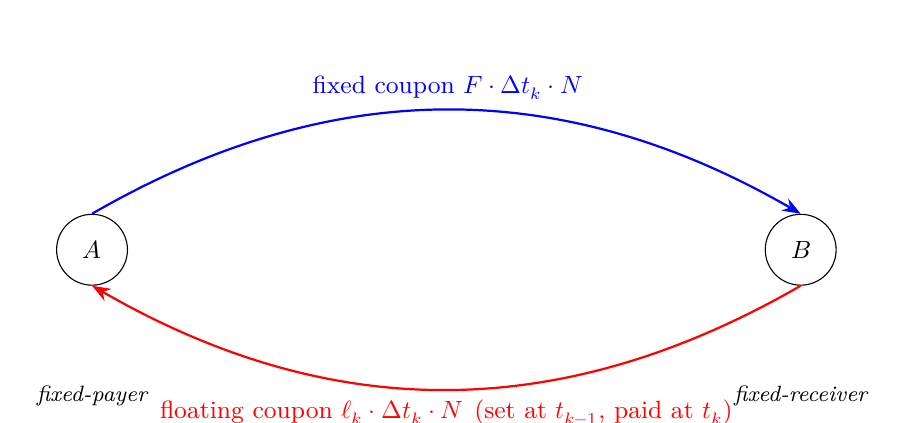
\begin{tikzpicture}[>=Stealth,scale=1.0,every node/.style={font=\small}]
  \node[circle,draw,minimum size=0.9cm] (A) at (0,0) {$A$};
  \node[circle,draw,minimum size=0.9cm] (B) at (9,0) {$B$};
  \draw[->,thick,blue] (A.north) to[bend left=30] node[above,midway] {fixed coupon $F \cdot \Delta t_k \cdot N$} (B.north);
  \draw[->,thick,red] (B.south) to[bend left=30] node[below,midway] {floating coupon $\ell_k \cdot \Delta t_k \cdot N$\;\;(set at $t_{k-1}$, paid at $t_k$)} (A.south);
  \node[font=\footnotesize\itshape,below=1.6cm] at (A) {fixed-payer};
  \node[font=\footnotesize\itshape,below=1.6cm] at (B) {fixed-receiver};
\end{tikzpicture}

\textit{Notional $N$ never changes hands; only the netted coupon difference $(F - \ell_k)\cdot\Delta t_k\cdot N$ flows each period.}
\end{figure}

The payment schedule lives on the interval grid
\(t_0 < t_1 < \dots < t_n\) with ``first-reset'' at \(t_0\) (rate fixed
there) and ``first-payment'' at \(t_1\); subsequent coupons at
\(t_2, \dots, t_n\).

\textbf{Why swaps exist.} An IRS converts a floating liability into a
fixed one or vice versa --- a corporate treasurer pays fixed/receives
floating to lock funding cost; a mortgage bank receives fixed/pays
floating to match its floating funding. Cleared IRS notional is roughly
\$400--500 trillion, the largest derivative class by any measure.

\subsection{13.2.2 Pricing from the discount
curve}\label{pricing-from-the-discount-curve}

\textbf{Fixed-leg value.} Paying \(F \cdot N \cdot \Delta t_m\) at each
\(t_m\) has time-0 value

\[
V_0^{\text{fix}} \;=\; \sum_{m=1}^{n} \Delta t_m \, F \, N \, P_0(t_m)
\tag{13.1}
\]

The factor \(\sum_{m=1}^n \Delta t_m P_0(t_m)\) is the \textbf{annuity}
(or PVBP per unit rate). At time \(t\) before the swap matures, the
fixed leg value is \(V_t^{\text{fix}} = \sum_m F \Delta t_m P_t(t_m)\).

The annuity interpretation is worth dwelling on. Think of
\(\mathcal{A}_0 \equiv \sum_m \Delta t_m P_0(t_m)\) as the present value
of a stream of \$1 payments per year, on the coupon schedule, discounted
to today. It functions as the ``unit of account'' for swap rates: the
par swap rate \(F\) is quoted as the number such that
\(F \cdot \mathcal{A}_0\) equals the floating-leg value. Multiplying or
dividing by the annuity converts between dollars and per-annum rate
units. The annuity is also the natural numeraire for changing measure in
swaption pricing: under the ``annuity measure'' (the probability measure
under which the annuity is the numeraire), the par swap rate \(S_t\)
becomes a martingale, and the swaption collapses to
\(V_0 = \mathcal{A}_0 \cdot \mathbb{E}^{\mathcal{A}}[(S_T -
K)_+]\) --- a direct lognormal expectation in Black form.

\textbf{Floating-leg value via ``buy \$1 and roll''.} The floating
coupon \(\ell_k\) is locked in at each reset \(t_{k-1}\) from the simple
yield on a \(\Delta t_k\)-bond:

\[
P_{t_{k-1}}(t_k) \;=\; \bigl(1 + \Delta t_k \, \ell_k\bigr)^{-1}
\;\Longrightarrow\;
\ell_k \;=\; \frac{1}{\Delta t_k}\!\left(\frac{1}{P_{t_{k-1}}(t_k)} - 1\right).
\tag{13.2}
\]

The reset mechanism works like this: at each reset date \(t_{k-1}\), the
market quotes a simply-compounded rate for the upcoming period
\([t_{k-1},
t_k]\), and that rate is fixed as the floating coupon for that period.
The coupon \(\ell_k \Delta t_k N\) is then paid at \(t_k\). So floating
coupons are \emph{set in arrears}, meaning the \(k\)-th coupon is known
at the \((k-1)\)-th reset and paid at \(t_k\). Standard LIBOR (and its
SOFR successor) follow this ``set-in-advance, paid-in-arrears''
convention, and (13.2) is the algebraic identity that makes replication
of the floating leg possible.

\textbf{Claim:} \(V_t^{\text{fl}} = \bigl(P_t(t_0) - P_t(t_n)\bigr) N\).

\emph{Financial argument (self-financing replication).} Consider the
trader who at \(t_0\) is handed \$1 and asked to replicate the
floating-leg coupons:

\begin{itemize}
\tightlist
\item
  At \(t_0\): buy \$1-worth of \(t_1\)-bonds --- holdings
  \(1/P_{t_0}(t_1)\). These mature to \$\(1/P_{t_0}(t_1)\) at \(t_1\).
\item
  At \(t_1\): take \$1 of that and buy \(t_2\)-bonds: \(1/P_{t_1}(t_2)\)
  units; pocket the remainder
  \(\bigl(1/P_{t_0}(t_1) - 1\bigr) = \ell_1 \Delta t_1\).
\item
  Continue to \(t_n\), pocketing \(\ell_k \Delta t_k\) each period and
  holding \$1 of fresh short-dated bonds.
\end{itemize}

The cash flows generated by this self-financing strategy are exactly the
floating-leg coupons, plus a terminal \$1 repayment we return. Cost =
\$1 in at \(t_0\) minus \$1 out at \(t_n\), priced today:

\[
V_0^{\text{fl}} \;=\; \bigl(P_0(t_0) - P_0(t_n)\bigr) \, N
\tag{13.3}
\]

The floating leg is \textbf{model-free}: neither \(\kappa\) nor
\(\sigma\) nor \(\theta(t)\) enters (13.3). The randomness cancels
pathwise. Post-2008, a multi-curve adjustment (``OIS discounting'' with
a tenor basis to SOFR/LIBOR accrual) keeps (13.3) approximately correct.

\subsection{13.2.3 The par (fair) swap
rate}\label{the-par-fair-swap-rate}

Setting \(V_0^{\text{fix}} = V_0^{\text{fl}}\) gives the rate
\(F^* \equiv S_0\) that makes the swap worth zero at inception:

\[
\boxed{\;F \;=\; \frac{P_0(t_0) - P_0(t_n)}
{\displaystyle \sum_{m=1}^{n} \Delta t_m \, P_0(t_m)}
\;\equiv\; S_0 \quad \text{(initial par swap rate)}\;}
\tag{13.4}
\]

The denominator is the annuity. Since both legs are priced off the
discount curve alone, the par swap rate is a ratio of discount factors
--- \textbf{no model required}.

\begin{figure}
\centering
\pandocbounded{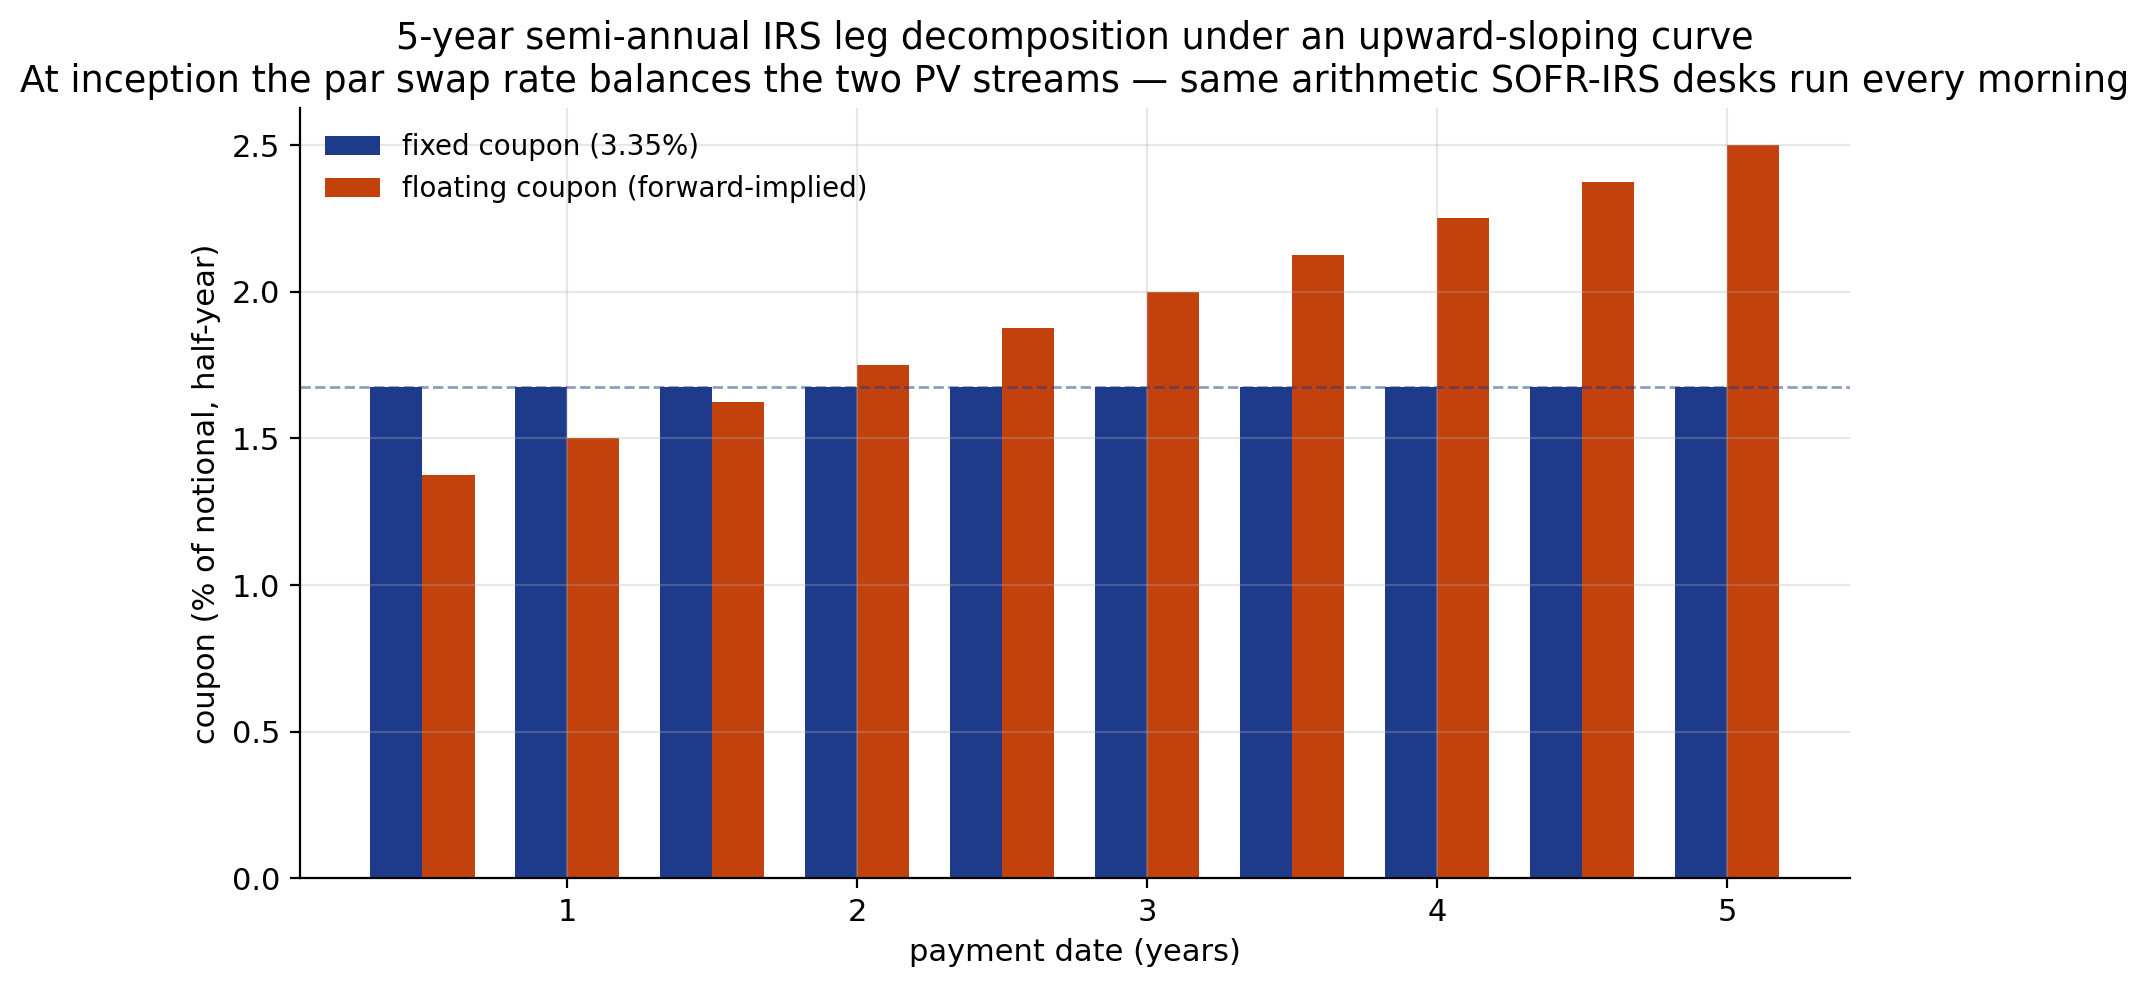
\includegraphics[keepaspectratio]{figures/ch13-swap-leg-decomposition.png}}
\caption{5-year semi-annual IRS leg decomposition under an
upward-sloping curve: fixed coupons at the par swap rate vs
forward-implied floating coupons. At inception the PVs balance --- the
basic arithmetic every SOFR-IRS desk runs to quote a 5y bid}
\end{figure}

The par swap rate \(S_0\) is the market's standard quote for ``the
\(n\)-year swap rate.'' When a Bloomberg screen shows ``10y USD swap is
3.5\%,'' that 3.5\% is \(S_0\) from (13.4) with \(n\) chosen to give a
10-year maturity. The swap curve --- the set of par swap rates across
tenors --- is directly observable and widely used as a reference
interest-rate curve for mortgages, corporate borrowing, and internal
bank funding.

\textbf{Swap rate \(\equiv\) par coupon yield.} Up to convexity
corrections, \(S_0\) equals the par coupon yield of a bond with the same
tenor. A par coupon bond with coupon \(c\) has PV
\(= c \cdot \mathcal{A}_0 + P_0(t_n)\), which equals par (notional)
exactly when \(c = (1 - P_0(t_n))/\mathcal{A}_0 =
S_0\). So ``a swap is a bond with no principal'' --- the coupon-rate
structure is identical; only the principal exchange differs.

\textbf{Forward-start / ongoing swap rate.} For a swap with payment
dates \(\{t_\ell\}_{\ell : t_\ell > t}\) viewed at time \(t\) (some
resets already happened), the current fair-value swap rate is

\[
S_t \;=\; \frac{P_t(t_{k_t}) - P_t(t_n)}
{\displaystyle \sum_{m = k_t + 1}^{n} \Delta t_m \, P_t(t_m)}
\tag{13.5}
\]

where \(k_t\) is the index of the most recent reset before \(t\). If
\(t < t_0\) (spot-start), \(P_t(t_{k_t}) = P_t(t_0)\) and (13.5) reduces
to (13.4) with \(P_t\) replacing \(P_0\).

Because discount factors are stochastic, \(S_t\) is a stochastic
process. Plotting it alongside the short rate \(r_t\) reveals very
different dynamics: \(S_t\) is smooth and moves with the yield curve,
while \(r_t\) is volatile and determines the floating coupons. In a
sense, \(S_t\) is a low-pass-filtered version of \(r_t\), weighted
toward the long end of the curve. Empirically, the 10-year swap rate
might move 5 bp on a given day while the overnight rate moves 25 bp ---
a 5:1 ratio, matching the Hull-White prediction that long-tenor yields
move less than short-tenor yields in response to short-rate shocks.

\subsection{13.2.4 Mark-to-market and swap
DV01}\label{mark-to-market-and-swap-dv01}

For off-par swaps (where the fixed coupon \(F\) differs from \(S_0\)),
the swap has non-zero initial PV. If \(F = 4.00\%\) versus a par of
\(S_0 =
4.49\%\), the fixed-payer pays below market so the swap has positive PV
to the fixed-payer:

\[
V^{\text{fp}}_0 \;=\; (S_0 - F) \cdot \mathcal{A}_0 \cdot N
\tag{13.6}
\]

In the example, \(V^{\text{fp}}_0 = (4.49\% - 4.00\%) \cdot 2.7532 \cdot
100\text{M} \approx \$1.35\text{M}\). This is the ``off-market
adjustment'' paid upfront in a typical trade. Market convention is to
trade at-par (no upfront) for most swaps; off-market swaps arise for
customised deals or for collapsing multiple existing positions into a
single trade.

\textbf{DV01.} The ``01'' (pronounced ``oh-one'' or DV01) is the change
in PV for a 1-bp parallel shift in rates. For a receiver swap, DV01
\(\approx
\mathcal{A} \times 0.0001 \times N\). For a 10-year \$100M swap with
annuity \(\mathcal{A} = 8.5\):

\[
\text{DV01} \;\approx\; 100\text{M} \times 8.5 \times 0.0001 \;=\; \$85{,}000 \text{ per basis point.}
\]

This is the single most important risk metric for IRS trading, and it is
directly the annuity-weighted notional. DV01 decomposes by tenor
(``bucket DV01'') to reveal which parts of the yield curve the portfolio
is exposed to. Hedging a swap portfolio requires matching the bucket
DV01s via positions in benchmark instruments (typically government-bond
futures, short-end deposits, and other swaps at standard tenors).
Mismatched DV01s lead to residual P\&L as the yield curve reshapes.

Related quantities: BPV (basis-point value, same as DV01), PV01 (present
value of a 1-bp change, same), 01 (trade-floor shorthand). The important
distinction is between ``parallel-shift'' DV01 (all tenors up 1 bp
together) and ``bucket'' DV01 (only one tenor moves 1 bp). Parallel DV01
is a portfolio-level summary; bucket DV01 is the detailed breakdown
needed for hedging.

\subsection{13.2.5 Worked example: a 3-year par
swap}\label{worked-example-a-3-year-par-swap}

With \(P_0(1) = 0.9592\), \(P_0(2) = 0.9177\), \(P_0(3) = 0.8763\) and
\(\Delta t_k = 1\):

\[
S_0 \;=\; \frac{1 - 0.8763}{0.9592 + 0.9177 + 0.8763}
\;=\; \frac{0.1237}{2.7532} \;\approx\; 4.49\%.
\]

The 3-year discount falls from 1.0 at \(t = 0\) to 0.8763 at \(t = 3\),
so roughly 12.4 cents are ``lost'' to discounting over three years.
Spread over three annual coupons with annuity 2.75, that works out to
4.49\% per annum. This exactly matches the yield-to-maturity of a 3-year
par coupon bond with coupon 4.49\% --- the swap rate \emph{is} the par
coupon yield.

\textbf{Cross-check via zero yields.} \(P_0(1) = 0.9592 = e^{-y_1}\)
gives \(y_1 =
-\ln 0.9592 \approx 4.17\%\). Similarly \(y_2 \approx 4.30\%\),
\(y_3 \approx
4.40\%\). So the zero-coupon curve is 4.17\% at 1y, 4.30\% at 2y, 4.40\%
at 3y --- gently upward-sloping. The par swap rate (4.49\%) is slightly
above the 3-year zero yield (4.40\%) because of the convexity implicit
in the coupon structure: a coupon bond receives coupons as well as
principal, and because coupons are smaller than the principal, their
yield must be slightly higher to equate PVs. This ``convexity premium''
between coupon bonds and zero-coupon bonds is a standard bond-math
result.

\pandocbounded{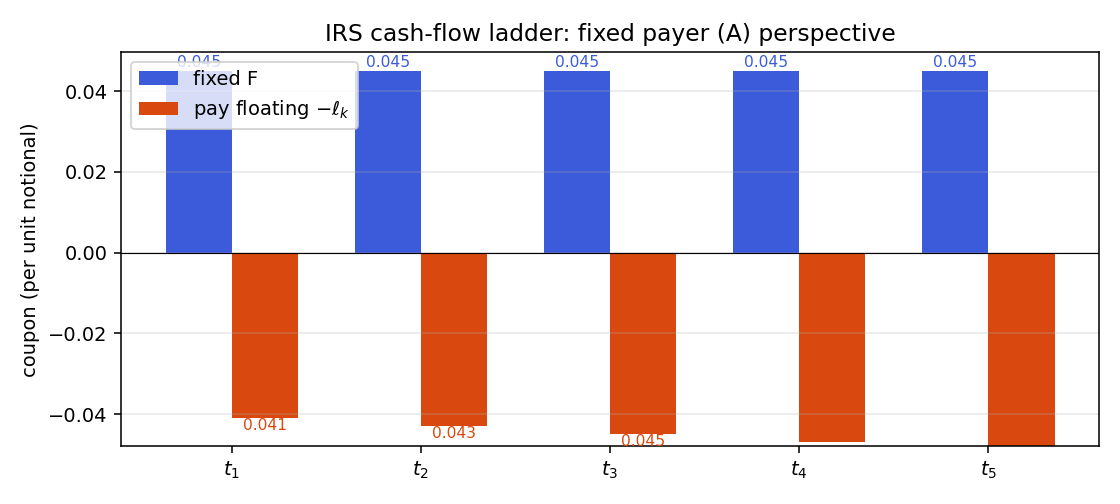
\includegraphics[keepaspectratio]{figures/ch05-irs-ladder.png}}
\emph{Fixed-payer sees outgoing blue fixed coupons and incoming orange
floating coupons; net PV is zero at the par swap rate \(S_0\).}

\begin{center}\rule{0.5\linewidth}{0.5pt}\end{center}

\subsection{Case study (a): LTCM 1998 --- swap spreads,
off-the-run/on-the-run,
leverage}\label{case-study-a-ltcm-1998-swap-spreads-off-the-runon-the-run-leverage}

\emph{Long-Term Capital Management --- Meriwether's Salomon arbitrage
group reincarnated, with Robert Merton and Myron Scholes on the
partnership and a Nobel Prize awarded mid-stream --- ran roughly
\(\$130\)B of balance sheet against \(\$4.7\)B of equity (Aug 1998
leverage ratio \(\approx 28{:}1\)), with one of the largest
concentrations being long-off-the-run / short-on-the-run Treasury basis
paired against IRS-spread positions. Russia's domestic-debt default on
\(17\) August 1998 destroyed both legs simultaneously and the equity
vanished in six weeks.}

\textbf{Context.} The trade rationale was simple §13.2 swap-curve
mathematics: the off-the-run Treasury (say, the previous-quarter issued
\(30\)y bond) trades at a small yield premium of \(5\)--\(10\) bp over
the most-recently-issued on-the-run, reflecting the on-the-run's
superior repo specialness and dealer demand. Over the bond's seasoning
life this premium compresses to zero, generating a \(5\)--\(10\) bp
risk-free convergence. LTCM ran the trade in size: long off-the-run,
short on-the-run (matched DV01), and frequently overlaid with a
pay-fixed IRS to monetise the swap-Treasury basis as well. Each
individual position had small daily P\&L variance, but the book was
scaled by leverage to produce target returns: portfolio DV01 in the
\(\$40\)--\(60\)M per basis point range against the \(\$4.7\)B equity
base. Internal \(99\%\) \(1\)-day VaR sat near \(\$45\)M --- about
\(1\%\) of equity.

The Russian default did not move the swap-Treasury basis by a small
amount; it moved it by \(30\) bp in the wrong direction in a single week
and another \(30\) bp the following month. Flight-to-quality bid up the
on-the-run Treasury (which is the most liquid hedge instrument in a
panic) while dumping the less-liquid off-the-run, widening the very
basis the trade was short. Simultaneously the swap spread --- the IRS
rate minus the corresponding-maturity Treasury --- widened to historic
levels: \(10\)y swap spreads went from \(\sim 35\) bp pre-crisis to
\(\sim 90\) bp by late September, briefly tagging \(200\) bp in some
tenors. With portfolio DV01 around \(\$50\)M/bp, the \(60\) bp basis
widening alone equalled \(\$3.0\)B in mark-to-market losses; aggregated
across all the convergence positions the fund lost \(\$4.6\)B of its
\(\$4.7\)B equity in six weeks. The Federal Reserve organised a
\(\$3.625\)B private-sector recapitalisation on \(23\) September to
prevent a forced liquidation that would have shocked counterparty banks.

\textbf{Reading it through the chapter's math.} The par swap rate (13.4)
is model-free --- it is a discount-curve identity that holds regardless
of the short-rate dynamics. But the \emph{spread} between two rates
(off-the-run vs on-the-run, IRS vs Treasury) is a \emph{liquidity}
premium that no calibrated short-rate model in this chapter captures: it
is an artefact of how dealers fund inventory in repo markets, who is the
marginal buyer in a flight-to-quality, and what regulatory capital
weights apply to which instrument class. The swap-spread convergence
trade's PnL is approximately linear in the spread, with sensitivity
equal to the matched DV01 --- that piece is exactly the §13.2.4 DV01
calculation. What the chapter's framework captures \emph{correctly} is
the \(\Delta\)P\&L per basis-point move; what it cannot tell you is what
magnitude of move to stress against. LTCM's internal VaR used historical
correlations from \(1995\)--\(1998\) --- a benign, low-vol period ---
under which off-the-run, IRS-Treasury, and Russian-bond moves were close
to independent. In crisis, they became a single one-factor
``flight-to-quality'' move and the gaussian VaR was off by a factor of
\(100\). Cornish-Fisher (Chapter 15, eq. (15.27)) would have helped only
if the third- and fourth-moment inputs themselves had been stressed;
they were not.

\textbf{Lesson.} The trade was \emph{correct on average} --- swap
spreads did mean-revert, and an unleveraged version of the position
would have been profitable across the cycle. The problem was the
\emph{path}: leverage transmits drawdowns into margin calls into forced
unwinds, and at \(28{:}1\) even a one-sigma move in the underlying
spread can wipe out equity if the move comes in a single week rather
than spread over a quarter. The deeper lesson for the new hire is that
DV01 measured against a normal-vol historical basis range is the wrong
risk metric for a leveraged convergence trade; the right metric is
``DV01 \(\times\) stressed move under a flight-to-quality scenario,''
and the stressed move is set by judgement about regime, not by a
covariance-matrix multiplier. Post-LTCM every prime broker tightened
margin financing for relative-value strategies; post-LTCM regulators
introduced stressed-VaR add-ons (Basel 2.5) that require the calibration
window to include \(1998\), \(2008\), or another comparable crisis
episode. The math of swap-spread arbitrage did not change after
\(1998\); the institutional discipline around leverage limits and
stressed-correlation scenarios did.

\begin{center}\rule{0.5\linewidth}{0.5pt}\end{center}

\section{13.3 Callable bonds on a short-rate
tree}\label{callable-bonds-on-a-short-rate-tree}

\subsection{13.3.1 Callable bond cash
flows}\label{callable-bond-cash-flows}

IRS pricing is essentially model-free, but a \textbf{callable bond} is a
genuinely model-dependent rate structure and the canonical application
of Hull-White numerical pricing. A callable bond is a fixed-coupon bond
that the issuer has the right (but not obligation) to redeem early at a
specified call price on one or more call dates. It is the bond-market
equivalent of a mortgage with a prepayment option --- the issuer can
refinance into a lower rate if rates fall.

Economically, a callable bond equals a straight (non-callable) bond
minus the issuer's call option:

\[
V^{\text{callable}}_t \;=\; V^{\text{straight}}_t \;-\; V^{\text{embedded call}}_t.
\tag{13.7}
\]

The issuer benefits if rates fall (they refinance at lower rates); the
bondholder loses the upside. So callable bonds trade at a \emph{higher}
yield than comparable straight bonds, with the spread representing the
option value. A 10-year callable with a 5-year first call might trade
30--80 bps above a comparable 10-year straight, with the spread widening
when rate volatility is high (because a more volatile world makes the
call option more valuable).

The yield differential is called the \textbf{option-adjusted spread
(OAS)}. It is the spread earned per year for being ``short the call'' as
a bondholder. If OAS is 50 bps, you are paid 50 bps per year to bear the
call-risk exposure. A useful way to think about the position: start with
a straight bond with clean duration-based pricing. Add in the issuer's
right to call (subtract the call option value). Now the bond's price is
lower and its \emph{effective} duration is lower --- because the bond
will likely be called early in a falling-rate scenario, shortening its
life. The \textbf{option-adjusted duration (OAD)} captures this
shortened effective life and is the correct hedge quantity for managing
the interest-rate risk of a callable-bond portfolio.

Pricing requires evaluating a max function at each call date:

\[
V^{\text{call}}_{t_c} \;=\; \min\!\bigl(\text{call price},\; V^{\text{continuation}}_{t_c}\bigr).
\tag{13.8}
\]

The issuer will call if the continuation value exceeds the call price
--- they pay off the bond for less than its market value. This is
\textbf{American-exercise optionality}, embedded in a rate-derivative
structure. No closed form exists in general; we must evaluate
numerically via a tree, lattice, or Monte Carlo with regression-based
exercise.

\subsection{13.3.2 Backward induction on a Hull-White trinomial
tree}\label{backward-induction-on-a-hull-white-trinomial-tree}

The standard approach is a Hull-White trinomial lattice. Build a tree
discretising \(r_t\) at each time step \(t_n\), with transition
probabilities calibrated to match the Hull-White moments. At each call
date, apply (13.8) at each node. Then roll back to \(t_0\) with standard
backward induction. The tree gives a complete price and, as byproducts,
the OAS (the yield spread over the discount curve that equates the tree
price to the market price) and the option-adjusted duration and
convexity.

\textbf{Construction sketch.} At each time \(t_n\), the short-rate state
is discretised to \(r^{(i)}_n\) for \(i = -m, \dots, +m\) (the tree has
\(2m + 1\) possible rate states). Transition probabilities to the three
successor states (up, middle, down) at \(t_{n+1}\) are calibrated to
match the first two conditional moments of \(r_{n+1} \mid r_n\) under
the Hull-White SDE. The mean reversion is handled by tweaking the
\emph{geometry} of the tree near the mean: at nodes where the standard
branching would require negative probabilities, the branching is tilted
(up-up-middle instead of up-middle-down, or the mirror) so all
probabilities stay in \([0, 1]\). This is the Hull-White (1994)
trinomial scheme --- robust, fast-converging, and standard in every
fixed-income pricing library.

A key feature is that the scheme handles the time-dependent
\(\theta(t)\) exactly: at each time step, the tree's drift is set to
match the calibrated \(\theta(t)\) at that time. So the tree
automatically incorporates the full curve-fit from the \(\theta\)
bootstrap from Chapter 12, without any additional work. This is the
computational payoff of the affine structure: calibration and pricing
both leverage the same underlying Gaussian geometry.

\textbf{Backward-induction algorithm.} Let \(V^{(i)}_n\) denote the
callable-bond value at node \((n, i)\). Work backward from maturity
\(T\):

\begin{enumerate}
\def\labelenumi{\arabic{enumi}.}
\tightlist
\item
  \textbf{Terminal condition} (\(n = N\)):
  \(V^{(i)}_N = \text{face} + \text{final
  coupon}\) at every node.
\item
  \textbf{Continuation value} (\(n < N\)): discount the expectation of
  the three successor values: \[
  V^{(i), \text{cont}}_n \;=\; e^{-r^{(i)}_n \Delta t}\bigl(p_u V^{(i+1)}_{n+1} + p_m V^{(i)}_{n+1} + p_d V^{(i-1)}_{n+1}\bigr) + c_n
  \] where \(c_n\) is the coupon paid at \(t_n\) (if any).
\item
  \textbf{Call test} (if \(t_n\) is a call date): apply
  \(V^{(i)}_n = \min\bigl(\text{call price}_n,\; V^{(i), \text{cont}}_n\bigr)\).
  Otherwise \(V^{(i)}_n = V^{(i), \text{cont}}_n\).
\item
  Continue to \(n = 0\); the callable price is \(V^{(0)}_0\) at the
  root.
\end{enumerate}

The algorithm is structurally identical to American-option pricing on a
stock tree, with the discount factor now state-dependent via
\(r^{(i)}_n\) rather than a constant \(r\). Each step is
\(O(\text{nodes at that time})\); total cost is \(O(N \cdot m)\) in
space and time, which is very fast even for dense calendars (quarterly
calls over 30 years).

\subsection{13.3.3 Decomposition into straight bond minus embedded
call}\label{decomposition-into-straight-bond-minus-embedded-call}

The accounting identity (13.7) can be verified numerically by running
the backward induction twice: once with the call test enabled (giving
the callable price), and once with the call test disabled (giving the
straight bond price). The difference is the value of the embedded call
option, which the issuer is short and the bondholder is long (as seen
from the issuer's liability side).

This decomposition is useful for \emph{Greeks}. The straight bond's
Greeks (duration, convexity) are well understood. The embedded call's
Greeks are what make callables complex --- and can be extracted from the
tree by finite-differencing the call-option value with respect to the
underlying rate curve, volatility, or time. The net callable Greeks are
then the straight-bond Greeks minus the call-option Greeks, mirroring
the value identity.

\textbf{Negative convexity.} A defining feature of callable bonds is
that OAD is \emph{non-monotonic} --- low near the call strike (the bond
is expected to be called soon), rising to the straight-bond duration far
from it. The OAD concavity is the ``negative convexity'' of callable
bonds. It forces dynamic rebalancing for hedgers and creates
duration-chasing feedback loops in the wider rate market (the canonical
MBS-convexity effect).

\begin{figure}
\centering
\pandocbounded{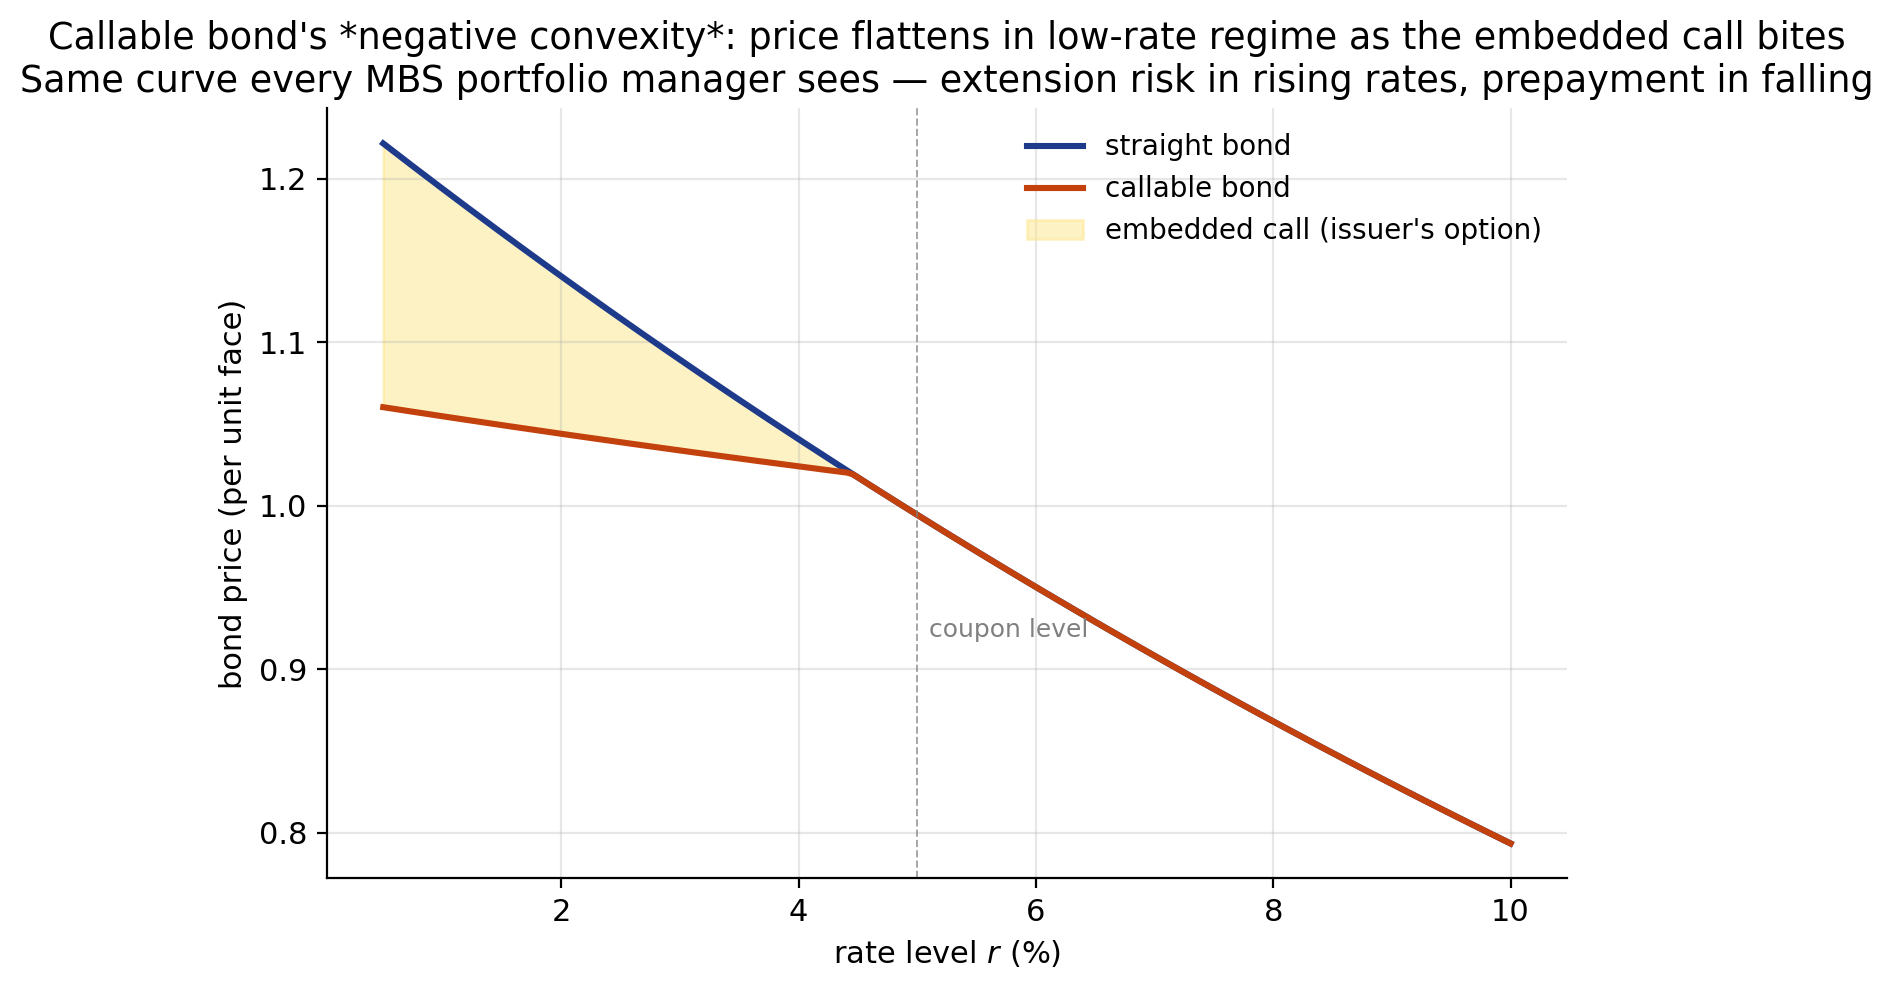
\includegraphics[keepaspectratio]{figures/ch13-callable-negative-convexity.png}}
\caption{Callable bond price vs straight-bond price across rate levels:
the embedded call value caps the callable's upside in low-rate regimes,
creating the characteristic ``negative convexity'' shape. Same effect
MBS portfolio managers manage on a daily basis as prepayment risk in
falling rates / extension in rising}
\end{figure}

\subsection{13.3.4 Numerical example}\label{numerical-example}

Take a 10-year bond with 5\% annual coupon, face value \$100, callable
annually at par (\$100) after year 3. Initial rate \(r_0 = 3\%\),
Hull-White parameters \(\kappa = 0.1\), \(\sigma = 0.015\), flat yield
curve at 3\% for simplicity. Build a trinomial tree of \(r\) values at
each year \(0, 1,
\dots, 10\) with transition probabilities calibrated to Hull-White. At
year 10, each node has \(V = \$105\) (principal + last coupon). Roll
back year-by-year, testing the call condition at years 3 through 9.

For parameters consistent with moderate vol, the callable bond might
price at \$105.20, compared to a straight bond at \$108.30. The embedded
call has value \$3.10, representing roughly 3\% of bond value. As
\(\sigma\) increases the call becomes more valuable and the callable
bond price falls further below the straight. This is the option-value
sensitivity: callable bonds are \textbf{short vega}, because they hold a
short call option.

Interpretation of the price: the callable's yield-to-worst is about
4.9\% (compared to a straight-bond yield of 4.1\%), so the callable
holder earns an extra 80 bps per year for bearing the call risk. In a
world where rates stay high, the issuer will not call (continuation
value stays below par), and the callable holder earns all the coupons.
In a world where rates fall, the issuer calls at par, and the holder
loses the future coupon stream. The 80 bps spread is the
probabilistically-weighted compensation for bearing this downside.

\textbf{Related products.} Putable bonds (holder owns the put),
convertible bonds (joint equity/rate model), and MBS (empirical
prepayment models on top of the lattice) all use the same
backward-induction skeleton. Calibrated \((\kappa, \sigma)\) from the
swaption market should feed the callable lattice --- under-calibrated
vol over-prices the bond.

\section{13.4 Credit default swaps}\label{credit-default-swaps}

\subsection{13.4.1 Default intensity, survival, and the protection
leg}\label{default-intensity-survival-and-the-protection-leg}

\textbf{Setup.} Protection buyer \(C\) pays periodic premium \(S\)
(annualised spread) to seller \(A\) on the reference name \(B\) until
default time \(\tau\). If \(\tau \le t_n\), the seller pays
loss-given-default \((1 - R) \, N\) at (or just after) \(\tau\), where
\(R\) is the recovery rate and \(N\) the notional. We model the default
time as the first jump of a Cox process; for this chapter
\(\tau \sim \text{Exp}(\lambda)\) with constant intensity \(\lambda\),
independent of the short rate, unless noted otherwise.

\begin{figure}[H]
\centering
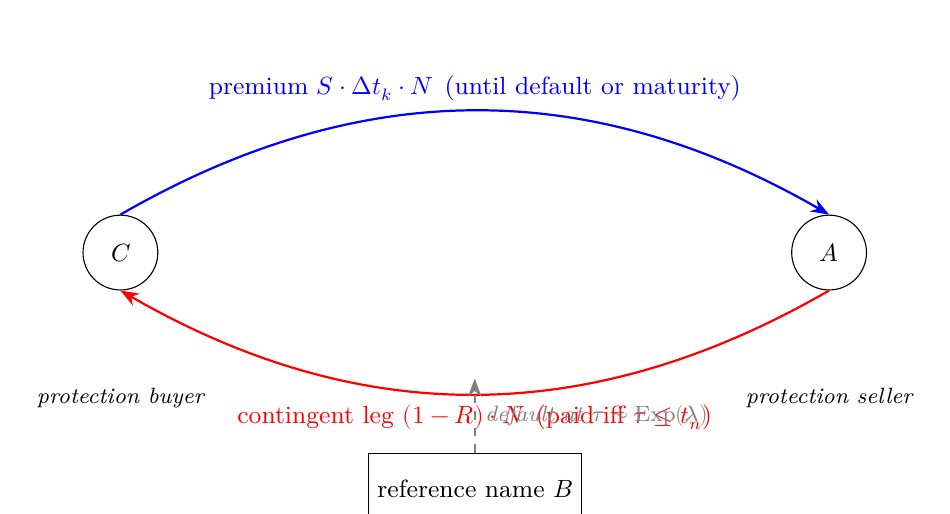
\begin{tikzpicture}[>=Stealth,scale=1.0,every node/.style={font=\small}]
  \node[circle,draw,minimum size=0.95cm] (C) at (0,0) {$C$};
  \node[circle,draw,minimum size=0.95cm] (A) at (9,0) {$A$};
  \node[rectangle,draw,minimum width=2.6cm,minimum height=0.9cm] (B) at (4.5,-3) {reference name $B$};
  \draw[->,thick,blue] (C.north) to[bend left=30] node[above,midway] {premium $S \cdot \Delta t_k \cdot N$\;\;(until default or maturity)} (A.north);
  \draw[->,thick,red] (A.south) to[bend left=30] node[below,midway] {contingent leg $(1-R)\cdot N$\;\;(paid iff $\tau \le t_n$)} (C.south);
  \draw[->,thick,gray,dashed] (B.north) -- (4.5,-1.6) node[midway,right,font=\footnotesize\itshape] {default at $\tau \sim \mathrm{Exp}(\lambda)$};
  \node[font=\footnotesize\itshape,below=1.6cm] at (C) {protection buyer};
  \node[font=\footnotesize\itshape,below=1.6cm] at (A) {protection seller};
\end{tikzpicture}

\textit{$C$ pays a stream of spreads; $A$ pays the loss-given-default once, at $\tau$, if it arrives before $t_n$.}
\end{figure}

\textbf{Economic picture.} A CDS is insurance against default. The
protection buyer pays a steady premium --- expressed as an annualised
spread \(S\) times the notional --- in exchange for a payout that
arrives if and only if the reference entity defaults before maturity.
This is economically equivalent to ``shorting the credit of the
reference name'': a long position in the bond plus a purchased CDS has
its default risk hedged out, leaving only rate-sensitivity exposure.

\textbf{Intensity, survival, and the hazard interpretation.} The
intensity \(\lambda\) has a sharp probabilistic meaning: for an
infinitesimal time interval \(\mathrm{d}t\), the probability of
defaulting in \([t, t + \mathrm{d}t]\) given no prior default is exactly
\(\lambda \, \mathrm{d}t\). So \(\lambda\) is the instantaneous default
rate, the \textbf{hazard rate}. In a flat-intensity world, the survival
probability is

\[
\mathbb{Q}(\tau > t) \;=\; e^{-\lambda t}
\tag{13.9}
\]

and the default distribution is exponential with mean \(1/\lambda\). A
typical investment-grade bond might have \(\lambda \approx 0.005\) per
year (50 bps hazard, 200-year expected survival); a junk bond might have
\(\lambda \approx 0.05\) (5\% hazard, 20-year expected survival).

The hazard-rate approach is a direct analog of the instantaneous-rate
approach to interest-rate modelling. Both use ``intensity'' as the
fundamental quantity. Both integrate the intensity to get the cumulative
quantity (integrated rate \(\to\) discount factor; integrated hazard
\(\to\) survival probability). Both admit time-varying intensities
(Hull-White \(\theta(t)\) for rates; stochastic hazard \(\lambda(t)\)
for credit) for realistic calibration.

\subsection{13.4.2 Premium and default legs; the par CDS
spread}\label{premium-and-default-legs-the-par-cds-spread}

\textbf{Premium leg.} Premium payments \(S \cdot \Delta t_\ell \cdot N\)
are paid on the schedule up to (and including the accrual period
containing) default:

\[
V_0^{\text{prem}} \;=\; S \cdot N \cdot \sum_{\ell=1}^{n} \Delta t_\ell \,
\mathbb{E}^{\mathbb{Q}}\!\left[\mathbf{1}_{\{\tau > t_\ell\}} \,
e^{-\int_0^{t_\ell} r_u \, \mathrm{d}u}\right]
\;=\; S \cdot N \cdot \sum_{\ell=1}^{n} \Delta t_\ell \, \widetilde{P}_0(t_\ell)
\tag{13.10}
\]

where \(\widetilde{P}_0(t_\ell) = e^{-\lambda t_\ell} \, P_0(t_\ell)\)
is the \textbf{risky discount factor} (survival \(\times\) riskless
ZCB). The sum \(\sum_\ell \Delta t_\ell \widetilde{P}_0(t_\ell)\) is the
\textbf{risky annuity}. Under independence of hazard and rate under
\(\mathbb{Q}\), the expectation factorises cleanly: otherwise
\(\widetilde{P}_0(t_\ell) = \mathbb{E}^{\mathbb{Q}}[e^{-\int_0^{t_\ell}
(r_u + \lambda_u) \, \mathrm{d}u}]\) which, for joint-Gaussian
\(r + \lambda\), again admits an affine closed form.

A heuristic: a risky bond earns the ``hazard-adjusted rate''
\(r + \lambda\) instead of just \(r\). The ``credit spread'' \(\lambda\)
is effectively an additional rate that the bond earns to compensate for
default risk. A corporate bond with a yield 150 bp above comparable
Treasury is earning \(r + 0.015\) in a flat-rate, flat-hazard world. The
150 bp is the credit spread, which the credit triangle (below) tells us
equals \((1 - R) \lambda\) approximately.

\begin{figure}
\centering
\pandocbounded{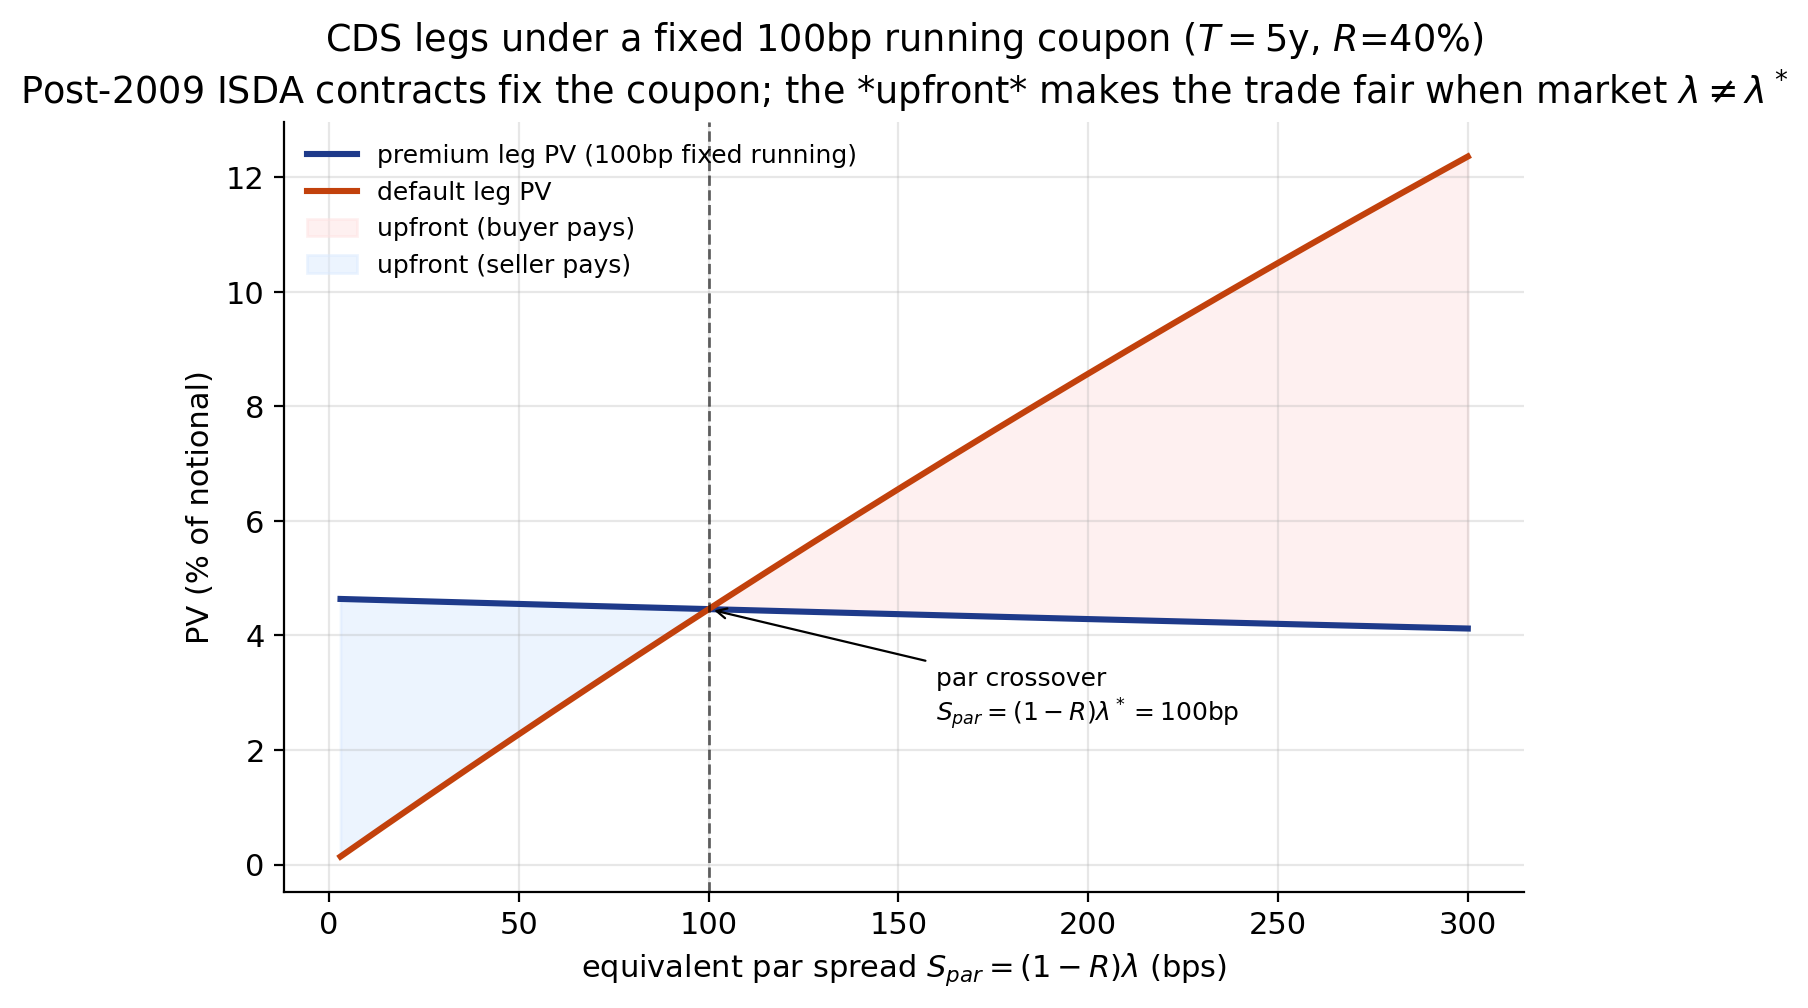
\includegraphics[keepaspectratio]{figures/ch13-cds-leg-balance.png}}
\caption{CDS legs under a fixed 100 bp running coupon: as market-implied
intensity \(\lambda\) moves, the premium leg stays flat (fixed coupon ×
annuity) while the default leg rises linearly. They cross at the par
intensity \(\lambda^*=S_{\text{run}}/(1-R)\) where upfront = 0; above
\(\lambda^*\) the buyer pays an upfront, below it the seller does ---
the post-2009 ISDA single-name quoting convention}
\end{figure}

\textbf{Default leg.} At default time \(\tau\), the payoff \((1 - R) N\)
is paid, discounted to \(t = 0\) via the riskless discount to \(\tau\).
Under independence of \(\tau\) and \(r\):

\[
V_0^{\text{D}} \;=\; \mathbb{E}^{\mathbb{Q}}\!\left[e^{-\int_0^{\tau} r_s \, \mathrm{d}s}
\, (1 - R) \, N \, \mathbf{1}_{\tau \le t_n}\right]
\;=\; (1 - R) \, N \int_0^{t_n}\!\lambda \, e^{-\lambda \tau} \, P_0(\tau) \, \mathrm{d}\tau.
\tag{13.11}
\]

The default density \(\lambda e^{-\lambda \tau}\) is the probability of
defaulting in \([\tau, \tau + \mathrm{d}\tau]\) per unit
\(\mathrm{d}\tau\); the present value of the loss is
\((1 - R) N P_0(\tau)\); the integration bound \([0, t_n]\) reflects
that the default leg pays only if default occurs before the contract
maturity.

The Markov property of Hull-White means that, conditional on \(r_\tau\),
the future bond price \(P_\tau(T)\) depends only on \((r_\tau, \tau, T,
\kappa, \sigma, \theta)\) --- not on history. So the post-default
discount \(P_\tau(T)\) is the Hull-White bond-price formula from Chapter
12 evaluated at shifted origin \(\tau\) and state \(r_\tau\). Under
independence of \(r\) and \(\lambda\), default timing is a purely
exponential process --- it does not care what the rate is doing --- so
integrating over default times first and then over rate paths gives the
same answer as doing them simultaneously. The pricing factorises.

\textbf{Par CDS spread.} Setting \(V_0^{\text{prem}} = V_0^{\text{D}}\)
at inception gives

\[
\boxed{\;S_0^{\text{CDS}} \;=\; \frac{(1 - R) \, \displaystyle \int_0^{t_n}\!\lambda \, e^{-\lambda \tau} \, P_0(\tau) \, \mathrm{d}\tau}
{\displaystyle \sum_{\ell=1}^{n} \Delta t_\ell \, \widetilde{P}_0(t_\ell)}\;}
\tag{13.12}
\]

Structurally this is (13.4) dressed up with survival probabilities: the
numerator is the PV of loss-given-default weighted by the default
density, the denominator is the risky annuity. The parallel between
(13.4) and (13.12) is not accidental: both are par-rate formulas for
insurance-like instruments. The structural similarity ``ratio of
value-generating leg to annuity-like leg'' recurs throughout rates and
credit markets.

\subsection{13.4.3 The credit triangle and worked
numbers}\label{the-credit-triangle-and-worked-numbers}

\textbf{The credit triangle.} In the limit of low hazard and short
maturity (so both survival \(e^{-\lambda t}\) and discount \(P_0(t)\)
are close to 1), the numerator of (13.12) integrates to approximately
\((1 - R) \lambda
t_n\) and the denominator to approximately \(t_n\), so

\[
S_0^{\text{CDS}} \;\approx\; (1 - R) \, \lambda
\quad\Longleftrightarrow\quad
\lambda \;\approx\; \frac{S_0^{\text{CDS}}}{1 - R}.
\tag{13.13}
\]

This is the single most important formula in credit trading. Given a
quoted CDS spread, extract the implied hazard rate by dividing by the
loss-given-default. With \(R = 40\%\) and a 100 bp CDS spread:
\(\lambda \approx 100/(1 - 0.4) = 167\) bp, implying a 1-year default
probability of \(1 - e^{-0.0167} \approx 1.65\%\). So a 100 bp CDS is
pricing in about 1.65\% default odds over the next year, 40\% recovery
if it happens. Every credit trader internalises the triangle: \emph{CDS
spread maps to hazard maps to default probability maps to
rating-equivalent.}

\textbf{Worked numerical example.} Take \(\lambda = 0.02\) (2\% hazard,
typical BBB), \(R = 0.4\) (40\% recovery), flat riskless curve at 3\%
for \(t_n = 5\) years with quarterly coupons (\(\Delta t_\ell = 0.25\)).

\begin{itemize}
\tightlist
\item
  Risky discount factors:
  \(\widetilde{P}_0(t_\ell) = e^{-(0.03 + 0.02) t_\ell} = e^{-0.05 t_\ell}\).
\item
  Risky annuity:
  \(\sum_{\ell=1}^{20} 0.25 \cdot e^{-0.05 \cdot 0.25 \ell} \approx 4.42\).
\item
  Default-leg integrand:
  \(\int_0^5 0.02 \cdot e^{-0.05 \tau} \, \mathrm{d}\tau \approx 0.0885\).
  Multiply by \((1 - R) = 0.6\): \(0.053\).
\item
  Par spread: \(0.053 / 4.42 \approx 120\) bp.
\item
  Credit-triangle approximation:
  \((1 - R) \lambda = 0.6 \cdot 0.02 = 120\) bp. Exact match for low
  hazard.
\end{itemize}

For a distressed \(\lambda = 0.10\) the exact formula gives
\textasciitilde610 bp vs the triangle's 600 bp --- the discounting
correction grows materially as \(\lambda\) rises.

\subsection{13.4.4 Bootstrapping the hazard-rate
curve}\label{bootstrapping-the-hazard-rate-curve}

Real-world hazards vary with the firm's health and the macro cycle.
Time- varying hazard \(\lambda(t)\) changes the survival formula to
\(S(t) = \exp(-\int_0^t \lambda(u) \, \mathrm{d}u)\), and the
default-leg integral generalises to

\[
V_0^{\text{D}} \;=\; (1 - R) \, N \int_0^{t_n}\!\lambda(\tau) \, S(\tau) \, P_0(\tau) \, \mathrm{d}\tau
\tag{13.14}
\]

Still a one-dimensional quadrature --- CDS pricing remains essentially
instantaneous on modern hardware.

\textbf{Typical calibration.} Given quoted CDS spreads at standard
tenors (1y, 3y, 5y, 7y, 10y), bootstrap a piecewise-constant hazard
curve \(\lambda(t)\) to match each spread exactly. This is the credit
analog of the Hull-White \(\theta(t)\) bootstrap from Chapter 12, and
the algorithm is analogous:

\begin{enumerate}
\def\labelenumi{\arabic{enumi}.}
\tightlist
\item
  Start at the shortest tenor (\(t_n = 1\)y) and pick \(\lambda_1\) so
  that (13.12) with constant \(\lambda = \lambda_1\) matches the 1y
  quote.
\item
  Move to the next tenor (\(t_n = 3\)y). With \(\lambda(t) = \lambda_1\)
  on \([0, 1]\) and \(\lambda(t) = \lambda_2\) on \([1, 3]\), pick
  \(\lambda_2\) so that (13.14) matches the 3y quote.
\item
  Continue tenor by tenor, building the full hazard schedule.
\end{enumerate}

The bootstrapped hazard curve is directly interpretable: \(\lambda_k\)
is the market-implied hazard for the bucket ending at tenor \(k\).
Upward- sloping credit curves (5y \textgreater{} 1y) imply increasing
hazard over time and are the norm for investment-grade names; inverted
curves (5y \textless{} 1y) signal near-term distress.

The \textbf{\(\mathbb{Q}\)-recovery} in the triangle is risk-neutral;
the \textbf{credit risk-premium multiplier} (\(\mathbb{Q}\)-hazard
\(\div\) \(\mathbb{P}\)-default rate) typically runs 2--4x for
investment-grade names, with direct implications for CDO tranche
pricing.

\subsection{13.4.5 CDS mark-to-market and
DV01}\label{cds-mark-to-market-and-dv01}

For off-par CDS (market spread has moved since inception), the mark-to-
market is the difference between premium and default legs evaluated at
current spread and current discount/hazard curves. ISDA conventions
since 2009 fix the \emph{coupon} at a standard 100 bp or 500 bp and
settle the spread-vs-coupon difference via an upfront payment:

\[
\text{Upfront} \;=\; \bigl(\text{market spread} - \text{fixed coupon}\bigr) \cdot \text{risky annuity} \cdot N.
\tag{13.15}
\]

Standardised fixed-coupon CDS with upfront payments make the CDS
fungible and centrally clearable, the post-2009 market structure.

\textbf{CDS DV01 and ``credit-DV01''.} Two sensitivities matter:

\begin{itemize}
\tightlist
\item
  \textbf{Rate DV01} (interest rate): sensitivity to a 1 bp parallel
  shift in the discount curve. Typically small (seconds-to-tens of
  dollars per \$1M notional) because rate effects largely cancel between
  the two legs.
\item
  \textbf{Credit-DV01} (spread): sensitivity to a 1 bp parallel shift in
  the hazard curve (or equivalently a 1 bp shift in the quoted spread).
  The dominant risk metric, equal to roughly \((1 - R) \cdot \text{risky
  annuity} \cdot N \cdot 0.0001\).
\end{itemize}

A \$10M 5y CDS with risky annuity 4.5 and 40\% recovery has credit-DV01
\(\approx \$10\text{M} \cdot 4.5 \cdot 0.6 \cdot 0.0001 = \$2{,}700\)
per basis point. A portfolio of dozens of names requires bucket
credit-DV01 by name and tenor, analogous to IRS bucket DV01 by tenor.

\pandocbounded{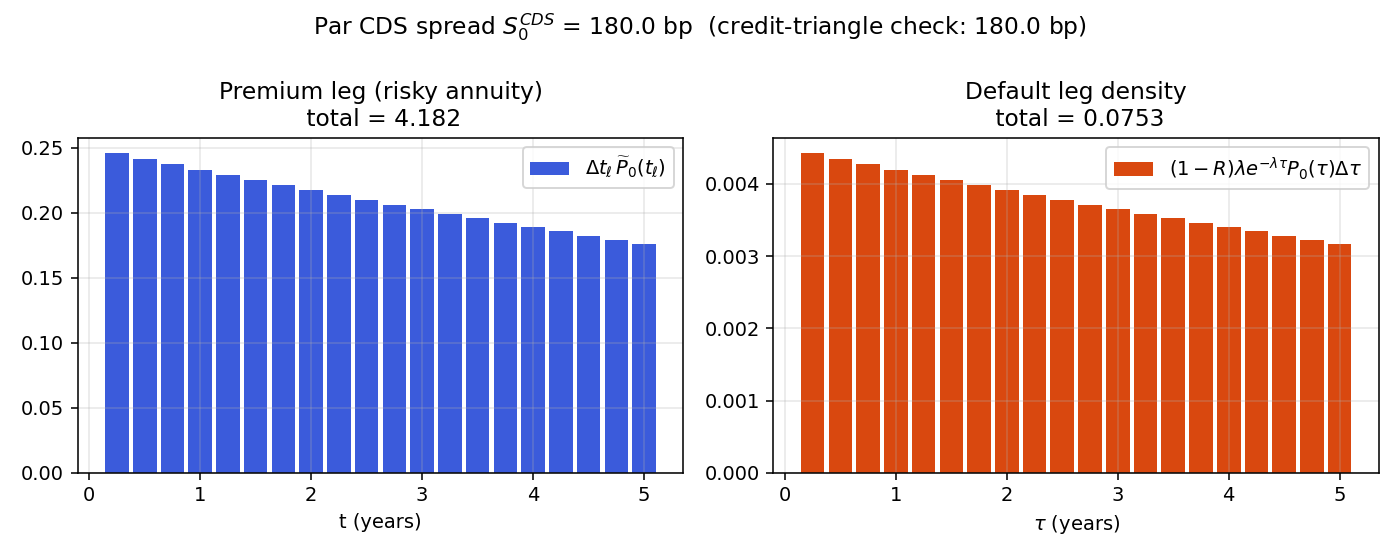
\includegraphics[keepaspectratio]{figures/ch05-cds-legs.png}}
\emph{The premium leg (left, blue) is a risky annuity. The default leg
(right, orange) is the probability-weighted loss density. At the par
spread the two areas match up to a factor of \(S_0^{\text{CDS}}\); the
credit triangle \((1-R)\lambda\) is the near-flat-curve limit.}

Production engines also handle accrued premium at default (a few-percent
correction to the premium leg, a few-bps on the par spread); we suppress
it here for clarity.

\section{13.5 The yield surface}\label{the-yield-surface}

\subsection{13.5.1 Spot, forward, and par-swap
surfaces}\label{spot-forward-and-par-swap-surfaces}

Before moving to bond options, we pause to visualise the object that
unifies everything the chapter has done so far: the \textbf{yield
surface} \(y_t(T)\), a 3D surface with axes \((t, T, y_t(T))\) showing
how the entire yield curve evolves over time. Under a calibrated
Hull-White model, at each sample date \(t\) we compute \(P_t(T)\) for a
range of \(T\) via the Chapter 12 bond-price formula evaluated at the
sampled \(r_t\), then invert \(y_t(T) = -\ln P_t(T)/(T - t)\).

The yield surface is the natural 3D object for a rates trader because it
makes explicit a distinction often blurred in text: the difference
between \textbf{calendar time} \(t\) (what the clock does) and
\textbf{maturity time} \(T\) (the endpoint of the bond). A 10-year yield
today and a 10-year yield one year from now are \emph{different bonds}:
one matures in 10 years, the other in 11 years from today's vantage.
Organising all this into a surface separates the two time dimensions
cleanly.

The surface is \textbf{smooth in \(T\)} (yields are smooth functions of
maturity via the affine exponent) but \textbf{rough in \(t\)} (driven by
stochastic \(r_t\)).

\subsection{13.5.2 One-factor signature and its
limits}\label{one-factor-signature-and-its-limits}

A one-factor model like Hull-White has a specific signature: all points
of the yield curve move together in response to a shock to \(r_t\), but
not by the same amount. A positive shock \(\delta r\) to \(r_t\) raises
the short end by the full shock magnitude and raises longer maturities
by the damped amount:

\[
\delta y_t(T) \;=\; \frac{B_{T-t}}{T - t} \cdot \delta r
\tag{13.16}
\]

For \(T - t\) short, \(B_{T-t}/(T - t) \approx 1\) and the yield moves
almost 1-for-1 with the shock. For \(T - t\) long,
\(B_{T-t}/(T - t) \approx 1/
(\kappa (T - t))\) and the yield moves by a damped factor. With
\(\kappa =
0.15\) and \(T - t = 30\) years, the damping factor is
\(1/(0.15 \cdot 30) =
0.22\): a 1 bp shock to \(r_t\) moves the 30-year yield by only 0.22 bp
in the model. This is a specific prediction of the one-factor structure.

In reality, the 30-year yield responds to short-rate shocks more
vigorously than one-factor Hull-White predicts --- typically by a factor
of 2-4\(\times\). Real-world rate shocks are often not just level
shocks; they come with concurrent slope shifts (inflation expectations,
policy stance). A pure level shock does damp out at the long end, but a
level- plus-slope shock can move the long end substantially. This is the
fundamental limitation of one-factor models and the motivation for
multi-factor extensions like G2++ and beyond (§13.8).

\textbf{No-arbitrage.} The Hull-White surface is no-arbitrage by
construction: the \(\mathbb{Q}\)-martingale condition on
\(e^{-\int r_u \,du} P_t(T)\) ties \(\theta(t)\) to the initial forward
curve (HJM drift condition, §13.8). This is why \(\theta(t)\)
calibration (Chapter 12) is a necessity, not a cosmetic choice.

\textbf{Bridge to §13.6.} The yield surface sets the stage for pricing
\emph{options} on the surface --- specifically, \textbf{European bond
options}, whose payoff depends on \(P_{T_0}(T_1)\), a single spot-yield
draw from the future surface at time \(T_0\). Pricing these options is
where the T-forward measure earns its keep.

\begin{center}\rule{0.5\linewidth}{0.5pt}\end{center}

\subsection{Case study (b): SVB collapse March 2023 --- duration
mismatch + held-to-maturity
accounting}\label{case-study-b-svb-collapse-march-2023-duration-mismatch-held-to-maturity-accounting}

\emph{Silicon Valley Bank, the \(16\)th-largest US bank by assets in
early \(2023\), failed in \(48\) hours between \(9\) March (deposit run
begins) and \(10\) March (FDIC takes the bank into receivership). The
proximate cause was that depositors discovered the bank's \(\$120\)B
held-to-maturity Treasury and agency-MBS portfolio carried an unrealised
mark-to-market loss of approximately \(\$15\)B against tangible common
equity of \(\$16\)B. The trade was unhedged duration; the failure was
governance.}

\textbf{Context.} During \(2020\)--\(2021\) SVB grew deposits
explosively as venture-funded startups parked cash from a record
fundraising cycle. Deposits roughly tripled, from \(\$60\)B at
end-\(2019\) to \(\$190\)B at peak-\(2022\). SVB invested the inflows in
long-duration safe assets: predominantly \(10\)y-and-longer agency MBS
and \(5\)y-and-longer Treasuries, purchased at the then-prevailing
yields of \(1.5\%\)--\(2.5\%\). The asset book carried
portfolio-weighted duration of approximately \(5.6\) years; the
liability side was overnight-redeemable deposits with effective duration
of zero. Asset-liability duration mismatch was thus around \(5.6\) years
against \(\$120\)B of HTM-classified assets.

The Federal Reserve raised the funds rate from \(0.00\)--\(0.25\%\) in
March \(2022\) to \(4.50\)--\(4.75\%\) by February \(2023\) --- a
parallel shift of approximately \(450\) basis points across the front of
the curve, with smaller but material moves at longer maturities (\(10\)y
Treasury yield went from \(\approx 1.5\%\) to \(\approx 4.0\%\), a
\(250\) bp move). SVB's HTM book was carried on the balance sheet at
amortised cost under ASC \(320\), which permits MTM losses to bypass
income provided the bank ``intends and has the ability'' to hold to
maturity. The MTM loss was disclosed in footnotes --- by Q\(4\) \(2022\)
filings, \(\sim \$15\)B unrealised loss against \(\sim \$16\)B equity
--- but did not flow through P\&L or regulatory capital. Once Silicon
Valley depositors (each covered up to only \(\$250\)k of FDIC insurance,
and most holding multiples of that) became aware of the gap, the deposit
run on Thursday \(9\) March forced SVB to start selling HTM assets,
crystallising losses, which accelerated the run, which closed the bank
by Friday morning. Subsequent receivership cost the FDIC's
deposit-insurance fund approximately \(\$20\)B.

\textbf{Reading it through the chapter's math.} The duration arithmetic
is the most elementary instance of §13.5 modified-duration analysis. For
a \(5\)-year zero-coupon bond, modified duration equals approximately
\(5\); the \(\Delta P/P \approx -D \cdot \Delta y\) approximation gives
a \(25\%\) MTM loss for a \(500\) bp parallel shift, \(22.5\%\) for
\(450\) bp. SVB's portfolio with weighted duration \(5.6\) on \(\$120\)B
HTM gives an order-of-magnitude loss estimate of
\(0.056 \times 0.045 \times \$120\)B \(\approx \$30\)B for a
hypothetical \(450\) bp parallel shift on duration-\(5.6\), but the
actual mark loss was \(\sim \$15\)B because (i) MBS carry negative
convexity that asymmetrically helps in a hiking cycle (extension
shortens prepayment-adjusted duration as rates rise), and (ii) some of
the portfolio matured into a flatter belly of the curve where the move
was smaller. DV01 (13.6) on the HTM book was thus approximately
\(\$70\)M per basis point --- meaning a \(1\) bp parallel shift in
Treasury yields changed the mark-to-market value of SVB's HTM book by
\(\$70\)M, or roughly \(0.4\%\) of equity, \emph{every basis point}. The
chapter-wide Hull-White machinery (Chapter 12 calibrated bond curve plus
this chapter's duration-convexity decomposition) would have computed
this exposure in seconds; nothing about the math was difficult or
unknown.

\textbf{Lesson.} SVB's failure was not a failure of interest-rate risk
\emph{math} --- duration of a \(5\)y zero is \(5\), and any sophomore
studying §13.5 can compute the implied MTM loss for any parametric
shift. It was a failure of interest-rate risk \emph{governance}: the
institutional choice to use HTM accounting suppressed the
\emph{visibility} of the loss without changing the \emph{risk} one bit.
When depositors marked the book themselves and ran, the gap that had
been hidden in footnotes flowed straight to the equity capital. The
deeper lesson for the new hire is that accounting classifications (HTM,
AFS, trading) are regulatory reporting choices; the underlying duration
risk is invariant to the accounting treatment, and any liquidity stress
that forces realisation will surface the loss regardless of which bucket
the position sat in. Risk reports should \emph{always} include MTM
Greeks on HTM books, and liquidity stress tests should \emph{always}
assume HTM positions get realised at MTM under a deposit-run scenario.
Post-SVB, US bank regulators rapidly escalated stressed-VaR-style
scenario requirements for AFS-and-HTM books at sub-\(\$250\)B regional
banks (which had been exempted from the largest-bank framework), and the
Federal Reserve introduced the Bank Term Funding Program to allow banks
to borrow against HTM Treasuries at par to prevent forced realisations.
None of this changed the duration math; all of it changed the discipline
around translating duration math into liquidity planning.

\begin{center}\rule{0.5\linewidth}{0.5pt}\end{center}

\section{13.6 European bond options and the T-forward
measure}\label{european-bond-options-and-the-t-forward-measure}

\subsection{13.6.1 Why change to the T-forward
measure}\label{why-change-to-the-t-forward-measure}

\textbf{Setup.} A European call on a bond has payoff
\(\bigl(P_{T_0}(T_1) - K\bigr)_+\) paid at \(T_0\), where
\(t < T_0 < T_1\). Let \(\mathfrak{g}_t\) denote the call price process.
Risk-neutral pricing under the money-market numeraire \(M_t\):

\[
\mathfrak{g}_t \;=\; \mathbb{E}^{\mathbb{Q}}_t\!\left[\, e^{-\int_t^{T_0} r_s \, \mathrm{d}s} \, \bigl(P_{T_0}(T_1) - K\bigr)_+\,\right].
\tag{13.17}
\]

Under Vasicek or Hull-White, \(P_{T_0}(T_1) = \exp\bigl(A_{T_0}(T_1) -
B_{T_0}(T_1) \, r_{T_0}\bigr)\), so the integrand in (13.17) couples
\emph{two} random variables driven by the same short-rate path: the
discount factor \(e^{-\int_t^{T_0} r_s \, \mathrm{d}s}\) and the
terminal bond value \(P_{T_0}(T_1)\). Both are nonlinear functions of
\(r_{T_0}\) and both are highly correlated (when rates are high at
\(T_0\), the discount factor is small \emph{and} the bond is cheap).

A direct computation would require evaluating a 2-dimensional Gaussian
integral involving the product of an exponential, an indicator function
(from the max), and another exponential. Feasible, but ugly. The
\textbf{numeraire-change trick} below eliminates the stochastic discount
factor entirely, reducing the problem to a clean 1-dimensional Gaussian
integral that is precisely the Black-76 setup.

\subsection{13.6.2 The T-forward measure (summary from Chapter
5)}\label{the-t-forward-measure-summary-from-chapter-5}

Chapter 5 derived the T-forward measure once as the canonical
application of Girsanov's theorem: we will not re-derive it here. The
result we need is this.

\emph{(Result, from Chapter 5.)} Let \(P_t(T_0)\) be a positive traded
numeraire. Define the \textbf{T-forward measure}
\(\widetilde{\mathbb{Q}}_{T_0}\) by the Radon-Nikodym derivative

\[
\left.\frac{\mathrm{d}\widetilde{\mathbb{Q}}_{T_0}}{\mathrm{d}\mathbb{Q}}\right|_{\mathcal{F}_t} \;=\; \frac{P_t(T_0) / M_t}{P_0(T_0) / M_0}.
\tag{13.18}
\]

Under \(\widetilde{\mathbb{Q}}_{T_0}\), every traded asset divided by
\(P_t(T_0)\) is a martingale:

\[
\frac{\mathfrak{g}_t}{P_t(T_0)} \;=\; \widetilde{\mathbb{E}}^{T_0}_t\!\left[\,\frac{\mathfrak{g}_{T_0}}{P_{T_0}(T_0)}\,\right] \;=\; \widetilde{\mathbb{E}}^{T_0}_t\!\left[\,\mathfrak{g}_{T_0}\,\right]
\quad\text{(since }P_{T_0}(T_0) = 1\text{)}
\tag{13.19}
\]

and the \(\mathbb{Q}\)-Brownian motion \(\widehat{W}_t\) is transformed
to \(\widetilde{W}^{\,0}_t\) via

\[
\mathrm{d}\widetilde{W}^{\,0}_t \;=\; \mathrm{d}\widehat{W}_t \;+\; B_t(T_0) \, \sigma \, \mathrm{d}t.
\tag{13.20}
\]

The drift shift \(B_t(T_0) \sigma\) is the \(\mathbb{Q}\)-volatility of
the numeraire \(P_t(T_0)\) (with a sign flip, because bond prices move
\emph{inversely} to rates). This is the \textbf{convexity adjustment}
from changing measure, and it is the standard Girsanov prescription
(``shift by the numeraire's volatility'') derived in Chapter 5.

Hence

\[
\boxed{\;\;\mathfrak{g}_t \;=\; P_t(T_0) \, \widetilde{\mathbb{E}}^{T_0}_t\!\left[\,\bigl(P_{T_0}(T_1) - K\bigr)_+\,\right]\;\;}
\tag{13.21}
\]

The awkward stochastic discount factor \(e^{-\int r \, \mathrm{d}s}\) is
gone: it has been absorbed into the numeraire \(P_t(T_0)\), which is now
a deterministic quantity outside the expectation.

\textbf{Intuition --- why Black's formula works here.} Switching
numeraire to \(P_t(T_0)\) --- the bond that matures exactly when the
option pays --- solves the problem in one stroke:

\begin{itemize}
\tightlist
\item
  \(P_{T_0}(T_0) = 1\) by definition, so at option expiry the numeraire
  equals 1 and the ``discount factor'' at that instant simply vanishes.
\item
  The \textbf{forward bond} \(X_t \equiv P_t(T_1)/P_t(T_0)\) is a ratio
  of two traded assets divided by the numeraire --- hence a
  \(\widetilde{\mathbb{Q}}_{T_0}\)-martingale by construction.
\item
  In Vasicek/Hull-White, the ratio of two exponential-affine bond prices
  is itself exponential-affine in a \emph{deterministic} combination
  \(B_t(T_0) - B_t(T_1)\), so \(X_t\) has deterministic volatility and
  is exactly a driftless geometric Brownian motion.
\end{itemize}

Geometric Brownian motion + driftless + deterministic volatility is
precisely the setup of Black-76 (Black's 1976 commodity-futures
formula). The bond-option price collapses to a Black-type
\(\Phi(d_\pm)\) expression with the ``forward'' \(X_t\), the
``discount'' \(P_t(T_0)\), and the ``total variance''
\(\int_t^{T_0} \Sigma_s^2 \,
\mathrm{d}s\). The numeraire choice is not cosmetic --- it is what makes
the problem lognormal.

The deeper lesson: \emph{match your numeraire to your payoff, and the
payoff's underlying becomes a driftless martingale --- the Black setup.}

\subsection{\texorpdfstring{13.6.3 Forward bond price dynamics under
\(\widetilde{\mathbb{Q}}_{T_0}\)}{13.6.3 Forward bond price dynamics under \textbackslash widetilde\{\textbackslash mathbb\{Q\}\}\_\{T\_0\}}}\label{forward-bond-price-dynamics-under-widetildemathbbq_t_0}

By Itô applied to \(P_t(T_1) = e^{A_t(T_1) - B_t(T_1) r_t}\) using the
Hull-White SDE \(\mathrm{d}r_t = \kappa(\theta_t - r_t) \, \mathrm{d}t +
\sigma \, \mathrm{d}\widehat{W}_t\) from Chapter 12:

\[
\frac{\mathrm{d}P_t(T_1)}{P_t(T_1)} \;=\; r_t \, \mathrm{d}t \;-\; \sigma \, B_t(T_1) \, \mathrm{d}\widehat{W}_t.
\tag{13.22}
\]

Every bond has \(\mathbb{Q}\)-drift \(r_t\) (consistent with being a
traded asset under the risk-neutral measure), with diffusion coefficient
\(-\sigma B_t(T_1)\). The minus sign reflects the inverse relationship
between bond prices and rates; the magnitude \(\sigma B_t(T_1)\) scales
with both the short-rate vol \(\sigma\) and the bond's duration
\(B_t(T_1)\). For a short bond (\(B \approx 0\)) the diffusion
coefficient is tiny; for a long bond it saturates at \(\sigma/\kappa\).
This is the Vasicek analogue of the duration-based bond-price volatility
heuristic.

Critically, in Vasicek/Hull-White, the bond's diffusion coefficient
\(-\sigma B_t(T_1)\) is \textbf{deterministic} --- it depends on time
and maturity but not on any random state variable. This is special to
Gaussian models. In CIR, the short-rate volatility \(\sigma\sqrt{r_t}\)
is state-dependent, and so is the bond's diffusion coefficient; the bond
is no longer lognormal under any measure change, and the resulting
bond-option formula is not of Black form (it involves a non-central
chi-squared distribution). The deterministic-volatility property is what
makes Vasicek bond options admit a Black-type closed form.

Under \(\widetilde{\mathbb{Q}}_{T_0}\), using (13.20) to substitute
\(\mathrm{d}\widehat{W}_t = \mathrm{d}\widetilde{W}^{\,0}_t - B_t(T_0) \sigma
\, \mathrm{d}t\), the \(T_1\)-bond's drift changes:

\[
\frac{\mathrm{d}P_t(T_1)}{P_t(T_1)} \;=\; \bigl(r_t + \sigma^2 B_t(T_0) \, B_t(T_1)\bigr) \, \mathrm{d}t \;-\; \sigma \, B_t(T_1) \, \mathrm{d}\widetilde{W}^{\,0}_t.
\tag{13.23}
\]

The drift correction \(+\sigma^2 B_t(T_0) B_t(T_1)\) is the
\textbf{convexity adjustment} from changing measure. Under
\(\mathbb{Q}\), the bond drifts at \(r_t\). Under
\(\widetilde{\mathbb{Q}}_{T_0}\), it drifts at a slightly higher rate,
by an amount proportional to the product of the two bonds' durations.
This extra drift keeps the \emph{ratio} \(P_t(T_1)/P_t(T_0)\) a
martingale, as required by the new numeraire choice.

The \emph{form} ``shift by the numeraire's volatility'' is universal
across continuous-diffusion models; the specific \(B_t(T_0)\sigma\) here
is just Vasicek's bond diffusion coefficient.

\begin{figure}
\centering
\pandocbounded{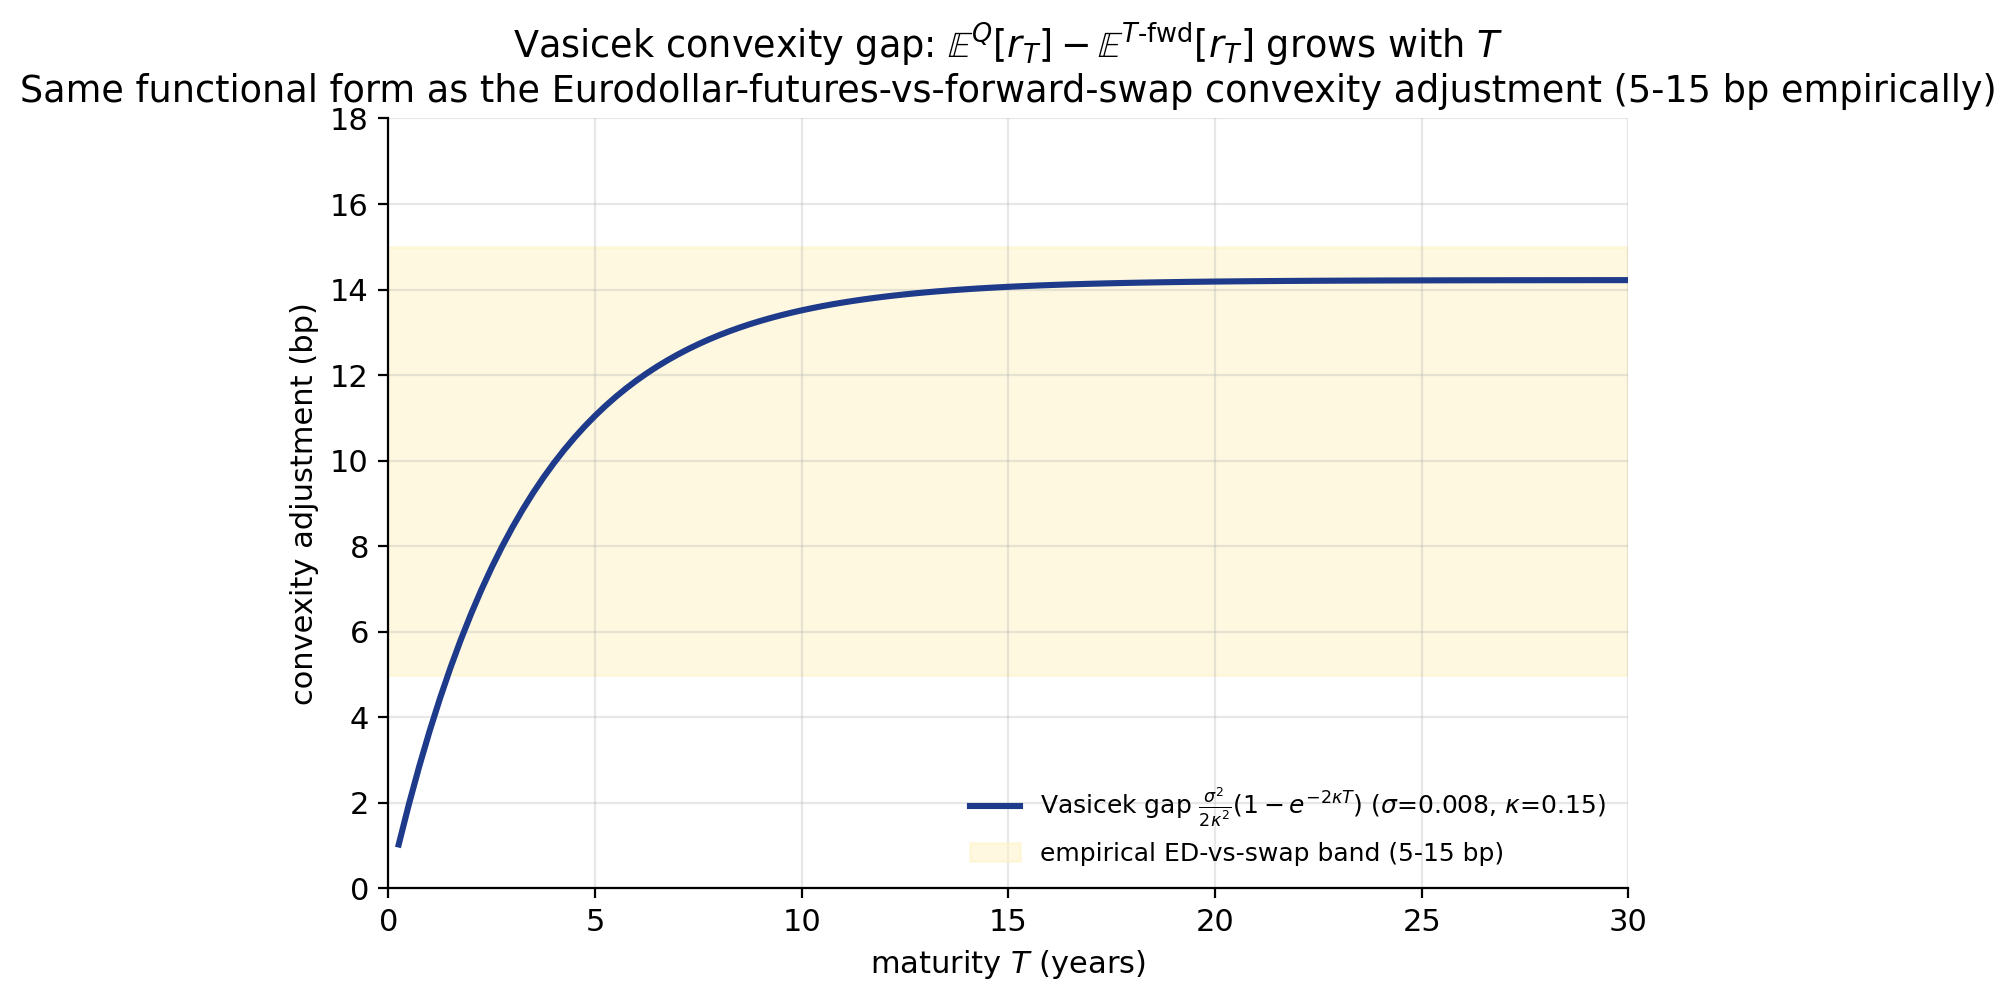
\includegraphics[keepaspectratio]{figures/ch13-convexity-adjustment.png}}
\caption{Vasicek convexity gap
\(\mathbb{E}^Q[r_T]-\mathbb{E}^{T\text{-fwd}}[r_T]=\frac{\sigma^2}{2\kappa^2}(1-e^{-2\kappa T})\)
at \(\sigma=0.008\), \(\kappa=0.15\), sitting inside the empirical 5--15
bp ED-vs-swap band (shaded). The ED-futures-vs-forward-swap convexity
has the same functional shape modulated by an additional
\(B(T_f,T_2)^2\) factor, hence the empirical match --- a non-trivial PnL
on multi-billion ED-vs-swap arbitrages}
\end{figure}

\pandocbounded{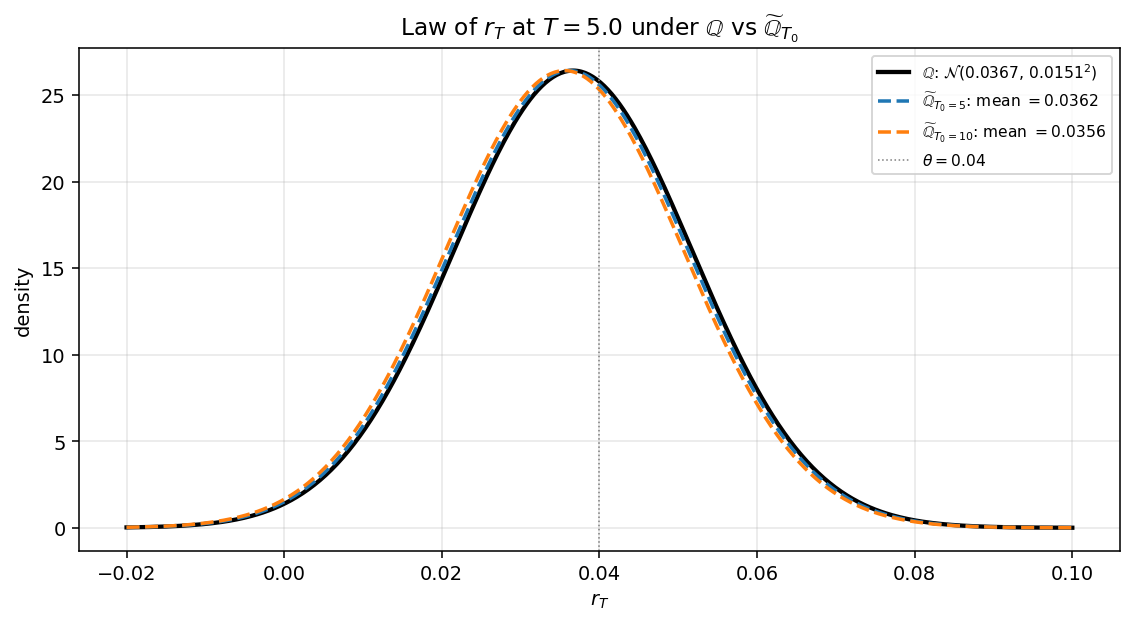
\includegraphics[keepaspectratio]{figures/ch11-rate-distributions.png}}
\emph{Changing numeraire from \(M_t\) to \(P_t(T_0)\) shifts the drift
of \(r_t\) downward by \(-\sigma^2 B_t(T_0)\): the conditional law of
\(r_{T_0}\) under the forward measure is a Gaussian with the same
variance but a lower mean than under \(\mathbb{Q}\). This shift is the
convexity adjustment relating forward rates to expected spot rates.}

\subsection{\texorpdfstring{13.6.4 Forward bond price \(X_t\) is a
\(\widetilde{\mathbb{Q}}_{T_0}\)-martingale}{13.6.4 Forward bond price X\_t is a \textbackslash widetilde\{\textbackslash mathbb\{Q\}\}\_\{T\_0\}-martingale}}\label{forward-bond-price-x_t-is-a-widetildemathbbq_t_0-martingale}

Introduce the \textbf{forward bond price}

\[
X_t \;=\; \frac{P_t(T_1)}{P_t(T_0)}.
\tag{13.24}
\]

Key boundary property:

\[
X_{T_0} \;=\; \frac{P_{T_0}(T_1)}{P_{T_0}(T_0)} \;=\; P_{T_0}(T_1),
\tag{13.25}
\]

so the option's payoff at \(T_0\) is exactly \((X_{T_0} - K)_+\).
\(X_t\) is a \(\widetilde{\mathbb{Q}}_{T_0}\)-martingale (ratio of
traded asset to numeraire).

By Itô on the ratio (both bonds driven by the same
\(\widetilde{W}^{\,0}\)):

\[
\frac{\mathrm{d}X_t}{X_t} \;=\; \sigma \, \bigl(B_t(T_0) - B_t(T_1)\bigr) \, \mathrm{d}\widetilde{W}^{\,0}_t \;\equiv\; \Sigma_t \, \mathrm{d}\widetilde{W}^{\,0}_t,
\tag{13.26}
\]

where the deterministic \textbf{forward-bond volatility} is

\[
\Sigma_t \;=\; \sigma \, \bigl(B_t(T_0) - B_t(T_1)\bigr) \;=\; -\frac{\sigma}{\kappa} \, e^{-\kappa T_0} \bigl(1 - e^{-\kappa(T_1 - T_0)}\bigr) \, e^{\kappa t}.
\tag{13.27}
\]

Only \(\Sigma_t^2\) appears below. The net exposure is
\textbf{deterministic} --- the property that makes Vasicek admit a
Black-type bond-option formula.

Because \(\Sigma_t\) is deterministic, \(X_t\) is a geometric Brownian
motion with deterministic volatility, and

\[
\boxed{\;\;X_T \;=\; X_t \, \exp\!\Bigl\{-\tfrac{1}{2}\!\int_t^T \Sigma_s^2 \, \mathrm{d}s \;+\; \int_t^T \Sigma_s \, \mathrm{d}\widetilde{W}^{\,0}_s\Bigr\}\;\;}
\tag{13.28}
\]

so \(\ln(X_T / X_t)\) is Gaussian under \(\widetilde{\mathbb{Q}}_{T_0}\)
--- a lognormal forward bond price.

\pandocbounded{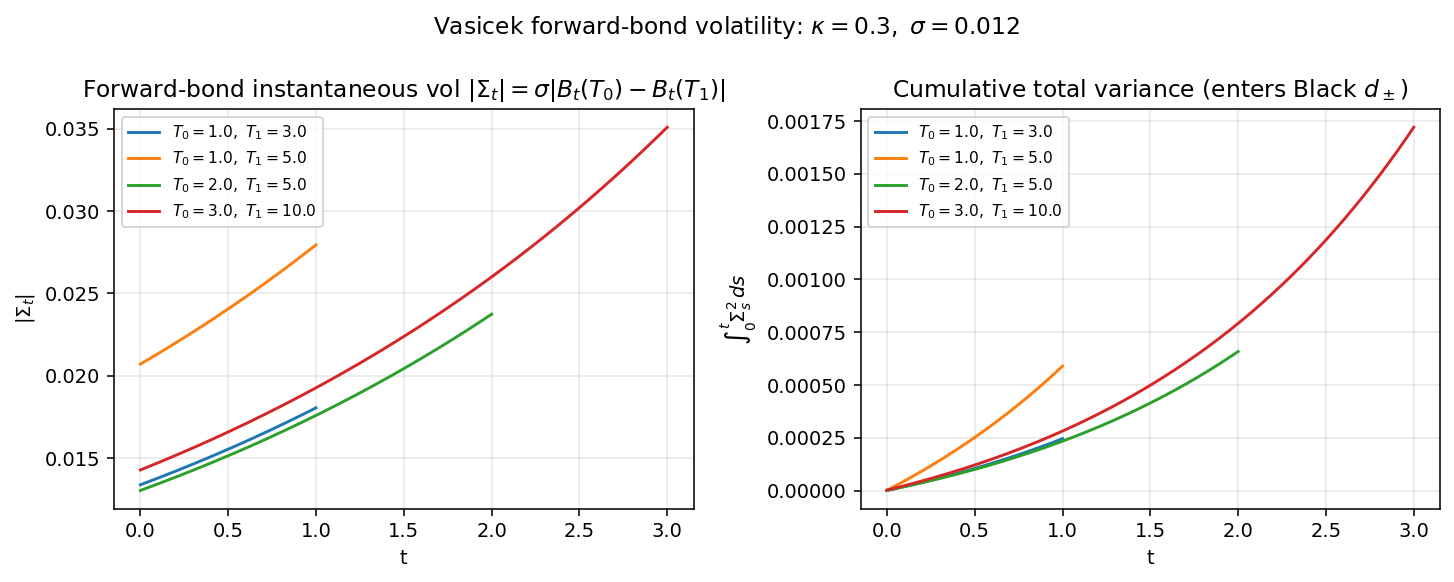
\includegraphics[keepaspectratio]{figures/ch11-forward-bond-vol.png}}
\emph{\(|\Sigma_t|\) grows as \(t \to T_0\) (the pull-to-par of
\(P_t(T_0)\) becomes less effective at absorbing rate noise); the
cumulative total variance \(\int_0^t \Sigma_s^2 \, \mathrm{d}s\) is what
appears in the Black \(d_\pm\) denominator.}

\subsection{13.6.5 Closed-form European bond call (Jamshidian /
Vasicek-Black)}\label{closed-form-european-bond-call-jamshidian-vasicek-black}

Plugging into (13.21):

\[
\mathfrak{g}_t \;=\; P_t(T_0) \, \widetilde{\mathbb{E}}^{T_0}_t\!\bigl[\,(X_{T_0} - K)_+\,\bigr].
\tag{13.29}
\]

This is a Black-style lognormal expectation with ``volatility''
\(\sqrt{\int_t^{T_0} \Sigma_s^2 \, \mathrm{d}s}\). Evaluating the
Gaussian integral in the standard way:

\[
\boxed{\;\;\mathfrak{g}_t \;=\; P_t(T_0) \, \bigl\{\,X_t \, \Phi(d_+) \;-\; K \, \Phi(d_-)\,\bigr\}\;\;}
\tag{13.30}
\]

with

\[
\boxed{\;\;d_\pm \;=\; \frac{\ln(X_t / K) \;\pm\; \tfrac{1}{2} \! \int_t^{T_0} \Sigma_s^2 \, \mathrm{d}s}{\sqrt{\int_t^{T_0} \Sigma_s^2 \, \mathrm{d}s}}\;\;}
\tag{13.31}
\]

This is the \textbf{Vasicek-Black bond-option formula}: a
Black-Scholes-type expression where the ``stock'' is the forward bond
\(X_t\), the ``discount factor'' is \(P_t(T_0)\), and the total variance
is the deterministic integral
\(\int_t^{T_0} \Sigma_s^2 \, \mathrm{d}s\).

\textbf{Boundary-condition check.} At expiry \(t = T_0\): the integral
\(\int_{T_0}^{T_0} \Sigma_s^2 \, \mathrm{d}s = 0\), so
\(d_\pm = \pm\infty
\cdot \mathrm{sgn}(\ln(X_{T_0}/K))\). Hence \(\Phi(d_+) - \Phi(d_-) =
\mathbf{1}\{X_{T_0} > K\}\), and the formula reduces to
\((X_{T_0} - K)_+ =
(P_{T_0}(T_1) - K)_+\), matching the contractual payoff. At deep OTM
strikes (\(K \gg X_t\)): both \(\Phi(d_+)\) and \(\Phi(d_-) \to 0\), and
the price goes to zero. At deep ITM (\(K \ll X_t\)):
\(\Phi(d_+) \to 1\), \(\Phi(d_-) \to 1\), and the price approaches
\(P_t(T_0)(X_t - K) =
P_t(T_1) - K P_t(T_0)\), the intrinsic value (forward value of bond
minus forward value of strike). All expected limits hold.

\textbf{Total-variance factorisation.} The integral admits a clean
closed form:

\[
\int_t^{T_0} \Sigma_s^2 \, \mathrm{d}s \;=\; \frac{\sigma^2}{\kappa^2} \, \bigl(1 - e^{-\kappa(T_1 - T_0)}\bigr)^2 \, \cdot \, \frac{1 - e^{-2\kappa(T_0 - t)}}{2\kappa}.
\tag{13.32}
\]

The three factors have clean physical interpretations:

\begin{itemize}
\tightlist
\item
  \(\sigma^2 / \kappa^2\): the overall \emph{scale}, roughly the
  stationary variance of \(r_t\) times 2.
\item
  \((1 - e^{-\kappa(T_1 - T_0)})^2\): the \emph{tenor-sensitivity}
  factor --- how much longer \(T_1\) is than \(T_0\).
\item
  \((1 - e^{-2\kappa(T_0 - t)})/(2\kappa)\): the \emph{time-to-expiry
  weighting}, saturating at \(1/(2\kappa)\) as \(T_0 - t \to \infty\).
\end{itemize}

Once these three numbers are computed for the relevant parameter grid,
pricing any Vasicek bond option is three multiplications plus a Black
formula --- a core rule-of-thumb for rates traders.

\subsection{13.6.6 Put-call parity for bond
options}\label{put-call-parity-for-bond-options}

\[
\mathfrak{g}_t^{\text{call}} - \mathfrak{g}_t^{\text{put}} \;=\; P_t(T_1) - K \, P_t(T_0).
\tag{13.33}
\]

Parity is the same as for equity options and is the cheapest sanity
check on a rates-option library.

\textbf{Digital bond options} --- options paying \$1 if
\(P_{T_0}(T_1) > K\) and 0 otherwise --- collapse to
\(\mathfrak{g}_t^{\text{digital}} = P_t(T_0) \cdot
\Phi(d_-)\). This is the Black-76 digital formula in disguise, useful
for structuring bespoke rate payoffs.

\section{13.7 Worked examples: Jamshidian decomposition and
Vasicek-Black}\label{worked-examples-jamshidian-decomposition-and-vasicek-black}

\subsection{\texorpdfstring{13.7.1 Worked example --- forward bond
volatility for a 1\times 3
option}{13.7.1 Worked example --- forward bond volatility for a 1 option}}\label{worked-example-forward-bond-volatility-for-a-1-option}

Suppose \(\sigma = 0.01\), \(\kappa = 0.3\), \(T_0 = 1\), \(T_1 = 3\).
From (13.32):

\begin{itemize}
\tightlist
\item
  \((1 - e^{-\kappa(T_1 - T_0)})^2 = (1 - e^{-0.6})^2 = (0.4512)^2 = 0.2036\)
\item
  \((1 - e^{-2\kappa T_0}) / (2\kappa) = (1 - e^{-0.6})/(0.6) = 0.7520\)
\item
  \(\sigma^2 / \kappa^2 = (0.01)^2 / 0.09 = 1.111 \times 10^{-3}\)
\end{itemize}

Total variance
\(\approx 1.111 \times 10^{-3} \cdot 0.2036 \cdot 0.7520 =
1.70 \times 10^{-4}\), so effective lognormal vol \(\approx \sqrt{1.70
\times 10^{-4}} = 1.30\%\).

Plug into (13.30)--(13.31) with \(X_0 = 0.94\) (forward bond price) and
strike \(K = 0.94\) (ATM). Then \(\ln(X_0/K) = 0\),
\(d_\pm = \pm \sqrt{1.70
\times 10^{-4}}/2 = \pm 0.00652\), \(\Phi(0.00652) = 0.5026\),
\(\Phi(-0.00652)
= 0.4974\). Call price:

\[
\mathfrak{g}_0 \;=\; P_0(1) \cdot \bigl(0.94 \cdot 0.5026 - 0.94 \cdot 0.4974\bigr) \;=\; P_0(1) \cdot 0.94 \cdot 0.0052 \;=\; 0.00489 \cdot P_0(1).
\]

For \(P_0(1) \approx 0.97\), the dollar ATM call price is about 0.00474,
or 47 bps of notional. Small premium --- consistent with short expiry
and modest vol --- but the right order of magnitude for a short-dated
ATM bond option.

\textbf{ATM approximation.}
\(\mathfrak{g} \approx P_0(1) X_0 \sigma_{\text{eff}}/\sqrt{2\pi} = 0.00473\)
--- matches exact Black to within 0.2\%. The
\(1/\sqrt{2\pi} \approx 0.4\) factor is the universal Black/Bachelier
ATM constant.

\subsection{13.7.2 ITM and OTM strikes}\label{itm-and-otm-strikes}

Returning to the 1\times 3 bond option with \(X_0 = 0.94\), consider an
ITM call (\(K = 0.90\)) and an OTM call (\(K = 0.98\)).

\textbf{ITM (\(K = 0.90\)).} \(\ln(X_0/K) = \ln(0.94/0.90) = 0.0435\).
With total variance \(1.70 \times 10^{-4}\), \(\sqrt{\cdot} = 0.01304\).
Then \(d_+ =
(0.0435 + 8.5 \times 10^{-5})/0.01304 = 3.34\), \(d_- = 3.33\).
\(\Phi(3.34)
\approx 0.9996\). Call price (per unit \(P_0(1)\))
\(= 0.94 \cdot 0.9996 -
0.90 \cdot 0.9996 = 0.04\). This is essentially the intrinsic value
(\(X_0 - K = 0.04\)); time value is tiny at such a deep-ITM strike and
short expiry.

\textbf{OTM (\(K = 0.98\)).} \(\ln(X_0/K) = -0.0417\). \(d_+ = -3.19\),
\(d_- = -3.20\). \(\Phi(-3.19) \approx 0.00071\). Call price
\(\approx X_0 \cdot 0.00071 -
K \cdot 0.00069 \approx 0\). The option is so deep OTM that the forward
bond has essentially no chance of reaching the strike in one year.

The asymmetry between ITM (near-intrinsic) and OTM (near-zero) is why
bond options trade like delta-one when far ITM and like pure gamma plays
when near ATM. Structured trades across strikes can achieve specific
exposure profiles: an ATM straddle gives pure gamma/vega; a wide-strike
strangle gives tail-event exposure.

\subsection{13.7.3 Sensitivity to mean-reversion
speed}\label{sensitivity-to-mean-reversion-speed}

Fix \(\sigma = 0.01\), \(T_0 = 1\), \(T_1 = 5\), and vary \(\kappa\):

\begin{itemize}
\tightlist
\item
  \(\kappa = 0.10\): \(\sigma^2/\kappa^2 = 0.01\), \((1 - e^{-0.4})^2 =
  0.1087\), \((1 - e^{-0.2})/0.2 = 0.9063\). Total var \(= 9.85 \times
  10^{-4}\), effective vol \(\approx 3.14\%\).
\item
  \(\kappa = 0.30\): \(\sigma^2/\kappa^2 = 1.11 \times 10^{-3}\), \((1 -
  e^{-1.2})^2 = 0.4968\), \((1 - e^{-0.6})/0.6 = 0.7520\). Total var \(=
  4.15 \times 10^{-4}\), effective vol \(\approx 2.04\%\).
\item
  \(\kappa = 1.00\): \(\sigma^2/\kappa^2 = 10^{-4}\), \((1 - e^{-4})^2 =
  0.9640\), \((1 - e^{-2})/2 = 0.4323\). Total var
  \(= 4.17 \times 10^{-5}\), effective vol \(\approx 0.646\%\).
\end{itemize}

Doubling \(\kappa\) from 0.10 to 0.30 cuts effective vol by
\textasciitilde1/3; \(\kappa = 1.0\) cuts it \textasciitilde80\%. The
dominant effect is \(\sigma^2/\kappa^2\) scaling like \(1/\kappa^2\).
Disentangling \((\kappa, \sigma)\) requires multiple option maturities:
short-expiry options are more sensitive to \(\sigma\), long-expiry to
\(\kappa\).

\pandocbounded{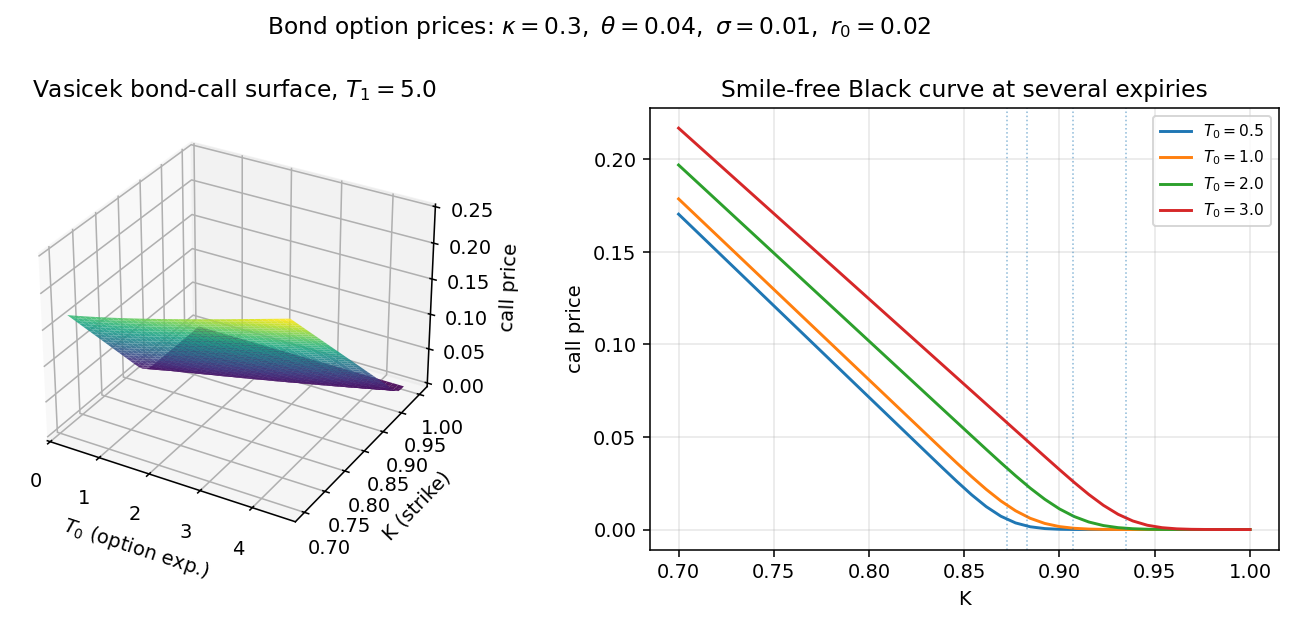
\includegraphics[keepaspectratio]{figures/ch11-bond-option-surface.png}}
\emph{Left: call price surface \(\mathfrak{g}_0(T_0, K)\) on a 5-year
zero via the Black-type Vasicek formula. Right: Black slices at fixed
\(T_0\) --- the dotted verticals mark the forward bond price
\(X_0 = P_0(T_1)/P_0(T_0)\) (ATM).}

\subsection{13.7.4 Jamshidian's decomposition: swaption as a portfolio
of bond
options}\label{jamshidians-decomposition-swaption-as-a-portfolio-of-bond-options}

A European \textbf{swaption} gives the right at \(T_0\) to enter a
fixed-floating swap with payments \(T_1 < \dots < T_N\). Its value at
\(T_0\) is a max of a sum of zero-coupon bond prices --- harder than an
option on a single bond.

\textbf{Jamshidian's 1989 insight.} In a one-factor Gaussian short-rate
model the sum of bond prices is monotone decreasing in \(r_{T_0}\), so a
unique critical rate \(r^*\) exists where the sum equals the strike. The
option on the sum decomposes into a portfolio of options on individual
bonds:

\[
\text{swaption}_0 \;=\; \sum_{i=1}^{N} c_i \cdot \text{BondOption}\bigl(T_0, T_i, K_i\bigr)
\tag{13.34}
\]

where \(c_i\) are the swap coefficients (tenors and notional), \(K_i =
P_{T_0}(T_i)\bigr|_{r = r^*}\) are effective strikes computed via the
Vasicek/Hull-White bond-price formula at \(r = r^*\), and \(r^*\) is the
critical rate obtained by solving a scalar equation.

\textbf{Procedure.}

\begin{enumerate}
\def\labelenumi{\arabic{enumi}.}
\tightlist
\item
  \textbf{Set up the critical-rate equation.} The swaption payoff at
  \(T_0\) is \((V^{\text{swap}}_{T_0} - K)_+\) where
  \(V^{\text{swap}}_{T_0} =
  \sum_i c_i P_{T_0}(T_i)\). Each \(P_{T_0}(T_i) = \exp(A_{T_0}(T_i) -
  B_{T_0}(T_i) r_{T_0})\) is a monotonically decreasing function of
  \(r_{T_0}\). So \(V^{\text{swap}}_{T_0}\) is monotonically decreasing
  in \(r_{T_0}\).
\item
  \textbf{Solve for \(r^*\).} Find the unique root of
  \(\sum_i c_i \exp(A_{T_0}(T_i) - B_{T_0}(T_i) r^*) = K\) --- a
  one-dimensional monotone root-find (bisection or Newton).
\item
  \textbf{Compute effective strikes.} For each \(i\), set
  \(K_i = \exp(A_{T_0}(T_i)
  - B_{T_0}(T_i) r^*)\).
\item
  \textbf{Price a portfolio of bond options.} Each term
  \(\text{BondOption}(T_0, T_i, K_i)\) is a Vasicek-Black call on the
  \(T_i\)-bond with strike \(K_i\), priced by (13.30)-(13.31).
\end{enumerate}

Jamshidian reduces an option-on-portfolio to a 1D root-find plus scalar
bond-option evaluations. Exact for one-factor Gaussian models; only
approximate (but useful as a starting point) for multi-factor. A
side-effect is flat-in-strike swaption vol under Vasicek; real swaption
smile motivates §13.8.

\subsection{13.7.5 Calibration pipeline}\label{calibration-pipeline}

The pipeline that ties the whole chapter together:

\begin{enumerate}
\def\labelenumi{\arabic{enumi}.}
\tightlist
\item
  \textbf{Fit \((\kappa, \sigma)\)} from swaption and/or cap quotes by
  minimising weighted least-squares between model-implied and market
  prices across the vol cube.
\item
  \textbf{Bootstrap \(\theta_t\)} from the initial bond curve (Chapter
  12) so that \(P_0^{\text{model}}(T) = P_0^{\text{market}}(T)\) for all
  \(T\).
\item
  \textbf{Price other rate derivatives} --- bond options via (13.30),
  swaptions via Jamshidian (13.34), callables via the Hull-White lattice
  (§13.3), caps/floors via strips of caplets (each a put on a
  zero-bond).
\end{enumerate}

Step 1's calibration is typically not unique: \((\kappa, \sigma)\)
combinations trade off ``persistent long-rate shocks'' (high \(\kappa\),
high \(\sigma\)) against ``temporary short-rate shocks'' (low
\(\kappa\), low \(\sigma\)). Short-expiry swaptions carry more
information about \(\sigma\); long-expiry about \(\kappa\). To resolve
degeneracy, practitioners often add long-dated cap vols or fix
\(\kappa\) at a historical value (say \(0.1\)) and only calibrate
\(\sigma\).

\section{13.8 Multi-factor preview: HJM, LMM, and
SABR}\label{multi-factor-preview-hjm-lmm-and-sabr}

\subsection{13.8.1 Why one factor is not
enough}\label{why-one-factor-is-not-enough}

One-factor Vasicek has four structural limits: perfect cross-maturity
correlation (real PCAs show 3 factors); limited curve shapes; flat
swaption smile (Jamshidian gives one vol per expiry-tenor); long-end
under-prediction (typical 2--4\times  gap). Each has a corresponding
remedy below.

\subsection{13.8.2 Two-factor Gaussian:
G2++}\label{two-factor-gaussian-g2}

The most common multi-factor extension of Vasicek is \textbf{G2++},
where the short rate is

\[
r_t \;=\; x_t + y_t + \phi(t)
\tag{13.35}
\]

with \(x_t\) and \(y_t\) two correlated Ornstein-Uhlenbeck factors:

\[
\begin{aligned}
\mathrm{d}x_t &= -a \, x_t \, \mathrm{d}t + \sigma_1 \, \mathrm{d}W^x_t, \\
\mathrm{d}y_t &= -b \, y_t \, \mathrm{d}t + \sigma_2 \, \mathrm{d}W^y_t, \\
\langle W^x, W^y\rangle &= \rho \, t,
\end{aligned}
\tag{13.36}
\]

\(\phi(t)\) is the deterministic curve-fit shift; one factor is
typically fast (short end), the other slow (long end); \(\rho\) controls
the curve shape. Bond prices remain exponential-affine:
\(P_t(T) = A(t,T)\exp(-B_1 x_t - B_2 y_t)\). Bond options are still
Black-type under the forward measure; Jamshidian holds only
approximately. G2++ can fit cap vols \emph{and} swaption vol cube at one
strike; real-market humped cap profiles drive negative-\(\rho\)
calibrations.

\subsection{13.8.3 HJM: modelling the entire forward
curve}\label{hjm-modelling-the-entire-forward-curve}

HJM (1992) takes the forward-rate curve \(f_t(T)\) as the primitive:
\(\mathrm{d}f_t(T) = \alpha(t,T)\,\mathrm{d}t + \sigma(t,T)\,\mathrm{d}W_t\),
with no-arbitrage forcing

\[
\alpha(t, T) \;=\; \sigma(t, T) \int_t^T \sigma(t, s) \, \mathrm{d}s.
\tag{13.39}
\]

Choosing \(\sigma(t,T)\) fully specifies the arbitrage-free dynamics.
Vasicek = exponential kernel; G2++ = sum of two. Generality costs
analytic tractability --- forward rates are rarely Markovian in low
dimensions, so most exotics need MC.

\subsection{13.8.4 LMM: the discrete-tenor LIBOR market
model}\label{lmm-the-discrete-tenor-libor-market-model}

LMM (BGM 1997 / Jamshidian) models a finite collection of forward LIBOR
rates as lognormal martingales under their own forward measures:
\(\mathrm{d}L_t^{(i)} = L_t^{(i)} \sigma_i(t)\,\mathrm{d}W^{(i)}_t\)
(13.40). It reproduces Black's caplet/swaption formula exactly for the
modelled forwards, at the cost of high-dimensional MC. The 2026-era RFR
LMM (SOFR, €STR, SONIA, TONA) replaces LIBOR with compounded overnight
rates.

\subsection{13.8.5 SABR and rate-vol
smile}\label{sabr-and-rate-vol-smile}

The models above (Vasicek, G2++, HJM, LMM) all produce a \emph{single}
implied volatility for each option --- no smile. Reality shows
substantial implied- vol smile in caps, floors, and swaptions: OTM
options trade rich of ATM, and the richness varies with strike in
specific ways (typically a negative skew for payers, reflecting the
asymmetry of rate distributions). Capturing this smile requires
stochastic-volatility or jump components.

The industry-standard overlay is \textbf{SABR} (Stochastic Alpha Beta
Rho), developed by Hagan and co-authors:

\[
\mathrm{d}F_t \;=\; \alpha_t \, F_t^\beta \, \mathrm{d}W_t, \qquad
\mathrm{d}\alpha_t \;=\; \nu \, \alpha_t \, \mathrm{d}Z_t, \qquad
\langle W, Z\rangle \;=\; \rho \, t.
\tag{13.41}
\]

\(\beta\) controls the backbone, \(\nu\) the vol-of-vol, \(\rho\) the
skew. The Hagan expansion gives a closed-form asymptotic implied vol ---
the industry standard quoting tool. SABR is per-strike/per-expiry (not
term-structure); the production stack is Hull-White / G2++ for the term
structure plus SABR per expiry-tenor.

\subsection{13.8.6 Where to use what}\label{where-to-use-what}

A rough practitioners' guide:

{\def\LTcaptype{none} % do not increment counter
\begin{longtable}[]{@{}
  >{\raggedright\arraybackslash}p{(\linewidth - 2\tabcolsep) * \real{0.4327}}
  >{\raggedright\arraybackslash}p{(\linewidth - 2\tabcolsep) * \real{0.5673}}@{}}
\toprule\noalign{}
\begin{minipage}[b]{\linewidth}\raggedright
Product
\end{minipage} & \begin{minipage}[b]{\linewidth}\raggedright
Recommended model
\end{minipage} \\
\midrule\noalign{}
\endhead
\bottomrule\noalign{}
\endlastfoot
Vanilla caps, floors, European swaptions & 1-factor Hull-White or G2++;
SABR overlay per strike \\
Bermudan swaptions, callable bonds & G2++ or LMM; Jamshidian-like
decomposition + MC for paths \\
CMS, LIBOR-in-arrears, convexity products & Multi-factor affine with
explicit convexity corrections \\
Path-dependent exotics (range accruals) & LMM or extended HJM, with
Monte Carlo \\
XVA (CVA/DVA/FVA) & G2++ for efficiency; hybrid with equity/credit
factors \\
Negative-rate environments & Vasicek/Hull-White/G2++ (Gaussian);
shifted-lognormal LMM \\
\end{longtable}
}

No single model dominates; desks maintain multiple models, switching per
product and regime. The mathematical apparatus is the common thread:
SDEs, Itô, Feynman-Kac, Girsanov, affine closed forms where they apply,
PDE-vs-MC where they don't.

\section{13.9 PDE versus Monte Carlo for rate
products}\label{pde-versus-monte-carlo-for-rate-products}

When closed forms are unavailable --- which is most of the time outside
vanilla caps, floors, and European swaptions --- one must resort to
numerical methods. The two main candidates are \textbf{PDE}
(finite-difference or finite-element) solvers and \textbf{Monte Carlo}
simulation. Each has strengths and weaknesses and the choice is
product-specific.

\subsection{13.9.1 When a PDE wins}\label{when-a-pde-wins}

PDE methods discretise the Feynman-Kac PDE on a grid in \((t, r)\) space
and solve backward via Crank-Nicolson. Output is the \emph{function}
\(g(t, r)\) on the grid, giving prices and all first-derivative Greeks
for free.

\begin{itemize}
\tightlist
\item
  \textbf{Strengths:} free Greeks; early-exercise natural
  (\(\max(g, \text{payoff})\)); deterministic.
\item
  \textbf{Weaknesses:} dimensional curse beyond 3--4 factors;
  boundary-condition fragility; path-dependence pushes dimensionality.
\end{itemize}

\subsection{13.9.2 When Monte Carlo wins}\label{when-monte-carlo-wins}

MC simulates paths and averages payoffs.

\begin{itemize}
\item
  \textbf{Strengths:} dimensional scaling (curse broken); path-dependent
  payoffs natural; parallelism on GPUs.
\item
  \textbf{Weaknesses:} slow convergence \(O(1/\sqrt N)\); Greeks need
  pathwise/likelihood-ratio/re-sim; early exercise via
  Longstaff-Schwartz.
\end{itemize}

\subsection{13.9.3 Practical guidance}\label{practical-guidance}

{\def\LTcaptype{none} % do not increment counter
\begin{longtable}[]{@{}ll@{}}
\toprule\noalign{}
Regime & Method \\
\midrule\noalign{}
\endhead
\bottomrule\noalign{}
\endlastfoot
1-factor + vanilla & PDE \\
2--3 factor + mildly exotic & PDE or MC \\
LMM/HJM / path-dependent & MC \\
XVA on large book & MC (often LS-MC for callables) \\
\end{longtable}
}

Hybrid methods (PDE-in-MC, Quasi-MC with Sobol, MLMC) handle edge cases.
The mathematics is unchanged across methods; only the numerical
implementation differs.

\section{13.10 Key takeaways}\label{key-takeaways-12}

\begin{enumerate}
\def\labelenumi{\arabic{enumi}.}
\item
  \textbf{Swaps are essentially model-free.} The floating leg
  self-replicates via ``buy \$1 and roll'':
  \(V_0^{\text{fl}} = (P_0(t_0) - P_0(t_n)) N\) --- no short-rate model
  required, only the discount curve. The par swap rate
  \(S_0 = (P_0(t_0) - P_0(t_n)) / \mathcal{A}_0\) is the ratio of that
  self-replicating value to the annuity; neither \(\kappa\) nor
  \(\sigma\) nor \(\theta_t\) appears.
\item
  \textbf{Callable bonds are genuinely model-dependent.} The embedded
  American option requires backward induction on a Hull-White trinomial
  tree with a call-value test at each exercise date: \(V^{\text{call}}
  = \min(\text{call price}, V^{\text{continuation}})\). OAS, OAD, and
  negative convexity emerge from the tree. Calibrated
  \((\kappa, \sigma)\) from the swaption market feed into the tree
  directly.
\item
  \textbf{CDS factor into a risky annuity and a default density.} The
  par CDS spread is
  \[S_0^{\text{CDS}} = \frac{(1 - R) \int_0^{t_n} \lambda e^{-\lambda \tau}
  P_0(\tau) \, \mathrm{d}\tau}{\sum_\ell \Delta t_\ell \widetilde{P}_0(t_\ell)}\]
  with \(\widetilde{P}_0(t) = e^{-\lambda t} P_0(t)\) the risky
  discount. The \textbf{credit triangle} \(S \approx (1 - R) \lambda\)
  is the low-hazard short-tenor limit and the most important formula in
  credit trading.
\item
  \textbf{T-forward measure eliminates stochastic discounting.} Changing
  numeraire from \(M_t\) to \(P_t(T_0)\) makes the discount factor
  deterministic at expiry (since \(P_{T_0}(T_0) = 1\)) and turns the
  forward bond \(X_t = P_t(T_1)/P_t(T_0)\) into a martingale with
  deterministic volatility \(\Sigma_t = \sigma(B_t(T_0) - B_t(T_1))\).
\item
  \textbf{Vasicek-Black bond-option formula.} A European call on a zero-
  coupon bond has the Black-76 form
  \[\mathfrak{g}_t = P_t(T_0) \bigl\{X_t \Phi(d_+) - K \Phi(d_-)\bigr\}\]
  with \(d_\pm\) computed from the deterministic total variance
  \(\int_t^{T_0} \Sigma_s^2 \, \mathrm{d}s = (\sigma^2/\kappa^2)(1 -
  e^{-\kappa(T_1 - T_0)})^2 \cdot (1 - e^{-2\kappa(T_0 - t)})/(2\kappa)\).
\item
  \textbf{Jamshidian decomposition reduces a swaption to a portfolio of
  bond options.} Exploit monotonicity of \(\sum_i c_i P_{T_0}(T_i)\) in
  \(r_{T_0}\): find the critical rate \(r^*\), compute effective strikes
  \(K_i\), and price each bond option by Black-76. Exact for one-factor
  Gaussian models; approximate but still useful for multi-factor.
\item
  \textbf{One-factor Vasicek is the start, not the destination.} G2++
  for curve richness, HJM for forward-curve primacy, LMM for direct
  forward-rate modelling, SABR for vol smile. Each extension fixes a
  specific limitation of the 1-factor Gaussian framework.
\item
  \textbf{PDE versus MC is a dimensionality trade-off.} PDE wins for 1-2
  factor vanilla products; MC wins for high-dimensional and path-
  dependent payoffs; hybrids handle edge cases. The underlying
  mathematics is unchanged --- only the numerical implementation
  differs.
\item
  \textbf{The chapter's unifying principle.} Every rate derivative
  prices as a conditional expectation of a payoff functional under the
  most convenient martingale measure. Match the numeraire to the
  payoff's natural scale, and the pricing collapses to a Black-type
  lognormal expectation. That sentence --- one idea --- ties every
  formula in this chapter together.
\end{enumerate}

\section{13.11 Reference formulas}\label{reference-formulas-8}

\subsection{Swaps}\label{swaps}

\[
\begin{aligned}
V_0^{\text{fix}} &= \sum_{m=1}^n \Delta t_m F N P_0(t_m) = F \cdot \mathcal{A}_0 \cdot N \\
V_0^{\text{fl}} &= (P_0(t_0) - P_0(t_n)) N \\
S_0 &= \frac{P_0(t_0) - P_0(t_n)}{\sum_m \Delta t_m P_0(t_m)} = \frac{P_0(t_0) - P_0(t_n)}{\mathcal{A}_0} \\
S_t &= \frac{P_t(t_{k_t}) - P_t(t_n)}{\sum_{m=k_t+1}^n \Delta t_m P_t(t_m)} \\
\text{DV01} &\approx \mathcal{A} \cdot 0.0001 \cdot N
\end{aligned}
\]

\subsection{Callable bonds (Hull-White
lattice)}\label{callable-bonds-hull-white-lattice}

Backward induction with call test:

\[
V^{(i)}_n = \begin{cases}
\min(\text{call price}_n, V^{(i), \text{cont}}_n) & \text{if } t_n \text{ is call date} \\
V^{(i), \text{cont}}_n & \text{otherwise}
\end{cases}
\]

where
\(V^{(i), \text{cont}}_n = e^{-r^{(i)}_n \Delta t}(p_u V^{(i+1)}_{n+1} +
p_m V^{(i)}_{n+1} + p_d V^{(i-1)}_{n+1}) + c_n\).

Value decomposition: \(V^{\text{callable}} = V^{\text{straight}} -
V^{\text{embedded call}}\).

\subsection{\texorpdfstring{CDS (constant hazard \(\lambda\) under
\(\mathbb{Q}\), independent of
\(r\))}{CDS (constant hazard \textbackslash lambda under \textbackslash mathbb\{Q\}, independent of r)}}\label{cds-constant-hazard-lambda-under-mathbbq-independent-of-r}

\[
\begin{aligned}
\widetilde{P}_0(t) &= e^{-\lambda t} P_0(t) \quad \text{(risky discount)} \\
V_0^{\text{prem}} &= S \cdot N \cdot \sum_\ell \Delta t_\ell \widetilde{P}_0(t_\ell) \\
V_0^{\text{D}} &= (1 - R) \cdot N \cdot \int_0^{t_n} \lambda e^{-\lambda \tau} P_0(\tau) \, \mathrm{d}\tau \\
S_0^{\text{CDS}} &= \frac{(1 - R) \int_0^{t_n} \lambda e^{-\lambda \tau} P_0(\tau) \, \mathrm{d}\tau}{\sum_\ell \Delta t_\ell \widetilde{P}_0(t_\ell)} \\
S &\approx (1 - R) \lambda \quad \text{(credit triangle, low } \lambda\text{)}
\end{aligned}
\]

Time-varying hazard: replace \(e^{-\lambda t}\) with \(S(t) =
\exp(-\int_0^t \lambda(u) \, \mathrm{d}u)\) and
\(\lambda e^{-\lambda \tau}\) with \(\lambda(\tau) S(\tau)\) inside the
default-leg integral.

\subsection{T-forward measure (cross-reference to Chapter 5 for Girsanov
derivation)}\label{t-forward-measure-cross-reference-to-chapter-5-for-girsanov-derivation}

\[
\left.\frac{\mathrm{d}\widetilde{\mathbb{Q}}_{T_0}}{\mathrm{d}\mathbb{Q}}\right|_{\mathcal{F}_t} = \frac{P_t(T_0)/M_t}{P_0(T_0)/M_0}
\qquad
\mathrm{d}\widetilde{W}^{\,0}_t = \mathrm{d}\widehat{W}_t + B_t(T_0) \sigma \, \mathrm{d}t
\]

\subsection{Bond SDE and forward bond}\label{bond-sde-and-forward-bond}

\[
\begin{aligned}
\frac{\mathrm{d}P_t(T)}{P_t(T)} &= r_t \, \mathrm{d}t - \sigma B_t(T) \, \mathrm{d}\widehat{W}_t \quad (\text{under } \mathbb{Q}) \\
X_t &= \frac{P_t(T_1)}{P_t(T_0)}, \qquad X_{T_0} = P_{T_0}(T_1) \\
\frac{\mathrm{d}X_t}{X_t} &= \Sigma_t \, \mathrm{d}\widetilde{W}^{\,0}_t, \qquad \Sigma_t = \sigma(B_t(T_0) - B_t(T_1))
\end{aligned}
\]

\subsection{European bond call
(Vasicek-Black)}\label{european-bond-call-vasicek-black}

\[
\mathfrak{g}_t = P_t(T_0) \bigl\{X_t \Phi(d_+) - K \Phi(d_-)\bigr\}
\qquad
d_\pm = \frac{\ln(X_t/K) \pm \tfrac{1}{2} \int_t^{T_0} \Sigma_s^2 \, \mathrm{d}s}{\sqrt{\int_t^{T_0} \Sigma_s^2 \, \mathrm{d}s}}
\]

\[
\int_t^{T_0} \Sigma_s^2 \, \mathrm{d}s = \frac{\sigma^2}{\kappa^2}(1 - e^{-\kappa(T_1 - T_0)})^2 \cdot \frac{1 - e^{-2\kappa(T_0 - t)}}{2\kappa}
\]

\subsection{Put-call parity for bond
options}\label{put-call-parity-for-bond-options-1}

\[
\mathfrak{g}_t^{\text{call}} - \mathfrak{g}_t^{\text{put}} = P_t(T_1) - K \cdot P_t(T_0)
\]

\subsection{\texorpdfstring{Jamshidian decomposition (swaption
\to  portfolio of bond
options)}{Jamshidian decomposition (swaption portfolio of bond options)}}\label{jamshidian-decomposition-swaption-portfolio-of-bond-options}

\[
\text{swaption}_0 = \sum_{i=1}^N c_i \cdot \text{BondOption}(T_0, T_i, K_i),
\qquad K_i = P_{T_0}(T_i)\bigr|_{r = r^*}
\]

with \(r^*\) solving
\(\sum_i c_i \exp(A_{T_0}(T_i) - B_{T_0}(T_i) r^*) = K\).

\subsection{Greeks for the bond call}\label{greeks-for-the-bond-call}

\[
\Delta = P_t(T_0) \Phi(d_+), \qquad
\Gamma = \frac{P_t(T_0) \phi(d_+)}{X_t \sqrt{\int_t^{T_0} \Sigma_s^2 \, \mathrm{d}s}}
\]

\[
\text{Vega} = \frac{\partial \mathfrak{g}_t}{\partial \sigma} = P_t(T_0) X_t \phi(d_+) \sqrt{\int_t^{T_0} \Sigma_s^2 \, \mathrm{d}s}/\sigma
\]

\subsection{Multi-factor and HJM}\label{multi-factor-and-hjm}

\[
\begin{aligned}
\text{G2++:} \quad & r_t = x_t + y_t + \phi(t), \qquad \mathrm{d}x_t = -a x_t \, \mathrm{d}t + \sigma_1 \, \mathrm{d}W^x_t \\
& \mathrm{d}y_t = -b y_t \, \mathrm{d}t + \sigma_2 \, \mathrm{d}W^y_t, \qquad \langle W^x, W^y\rangle = \rho \, t \\[4pt]
\text{HJM:} \quad & \mathrm{d}f_t(T) = \alpha(t, T) \, \mathrm{d}t + \sigma(t, T) \, \mathrm{d}W_t \\
& \alpha(t, T) = \sigma(t, T) \int_t^T \sigma(t, s) \, \mathrm{d}s \quad \text{(no-arb drift)} \\[4pt]
\text{LMM:} \quad & \mathrm{d}L_t(T_{i-1}, T_i) = L_t(T_{i-1}, T_i) \sigma_i(t) \, \mathrm{d}W^{(i)}_t \\[4pt]
\text{SABR:} \quad & \mathrm{d}F_t = \alpha_t F_t^\beta \, \mathrm{d}W_t, \qquad \mathrm{d}\alpha_t = \nu \alpha_t \, \mathrm{d}Z_t
\end{aligned}
\]

\subsection{Numerical methods --- choosing between PDE and
MC}\label{numerical-methods-choosing-between-pde-and-mc}

{\def\LTcaptype{none} % do not increment counter
\begin{longtable}[]{@{}ll@{}}
\toprule\noalign{}
Regime & Method \\
\midrule\noalign{}
\endhead
\bottomrule\noalign{}
\endlastfoot
1-factor vanilla & PDE (Crank-Nicolson) \\
2-3 factor vanilla/mild exotic & PDE or MC \\
High-dimensional (LMM, HJM) & Monte Carlo \\
American/Bermudan low-dim & PDE with min-test \\
American high-dim & Longstaff-Schwartz MC \\
XVA on large book & Monte Carlo (GPU) \\
Path-dependent exotic & Monte Carlo \\
\end{longtable}
}

\newpage

\chapter{Chapter 14 --- Caps, Floors, and
Swaptions}\label{chapter-14-caps-floors-and-swaptions}

\section{14.0 The rates-side capstone}\label{the-rates-side-capstone}

This chapter is the final application of the numeraire-change machinery
built earlier in the guide. In Chapter 5 we constructed the
Radon-Nikodym / Girsanov apparatus in full generality: every strictly
positive tradable defines a measure, forward measures in particular are
generated by zero-coupon bonds, and the annuity measure arises as a
portfolio-of-bonds numeraire. In Chapter 12 we built the short-rate
models --- Vasicek, Ho-Lee, Hull-White, and the general affine framework
--- that give us closed-form bond prices
\(P_t(T) = e^{A_t(T) - B_t(T)\,r_t}\) and explicit bond volatilities
\(B_t(T)\,\sigma\). In Chapter 13 we priced interest-rate swaps, CDS,
callable bonds, and European bond options, using the T-forward measure
as a cross-reference back to Chapter 5.

Caps, floors, and swaptions are the product set that ties all of this
together. A cap decomposes exactly, with no cross terms, into a strip of
single-date caplets, each priced as a Black-76 call under its own
T-forward measure \(\mathbb{Q}^{T_i}\). A swaption is irreducibly
multi-date, but under the annuity measure \(\mathbb{Q}^X\) the par swap
rate \(S_t\) becomes a single scalar martingale and the whole
\(n\)-dimensional bond-price problem collapses into a single Black call
on \(S\). Both moves are instances of the same general principle ---
pick a numeraire under which the underlying becomes a martingale and the
payoff factors cleanly --- and both are immediate applications of the
Girsanov theorem from Chapter 5. We do not re-derive the T-forward
measure or the change-of-Brownian-motion formula; we cite them. What is
new in this chapter is how they get used.

\begin{center}\rule{0.5\linewidth}{0.5pt}\end{center}

\section{14.1 Caps, Caplets, and the Interest-Rate
Swap}\label{caps-caplets-and-the-interest-rate-swap}

A cap is an interest-rate option made up of caplets. Caps/floors are
close cousins of swaptions (swap options). The easiest way to see where
a cap comes from is to start with its underlying --- a plain vanilla
interest-rate swap, as priced in Chapter 13 --- and ask what happens
when you put an option on the floating leg.

Consider a standard interest-rate swap (IRS) between counterparties A
and B on notional \(N\), with fixed leg \(F\) and floating leg \(\ell\):

\[
A \;\xrightleftharpoons[\ell]{F}\; B \qquad \text{(IRS)} \tag{14.1}
\]

In words, A pays fixed and receives floating; B pays floating and
receives fixed. The notional \(N\) never actually changes hands --- it
is simply a scale factor that multiplies the rate spread on each payment
date. Both legs are quoted as annualized rates, but each period's
payment applies only for the year-fraction \(\Delta t_k\) between
consecutive fixing/payment dates.

On the tenor grid \(t_0 < t_1 < t_2 < \dots < t_n\):

\begin{itemize}
\tightlist
\item
  Fixed leg pays \(F\,\Delta t_k\) at each \(t_k\), \(k = 1, \dots, n\).
\item
  Floating leg pays \(L_{t_{k-1}}(t_k)\,\Delta t_k\) at \(t_k\), where
  the rate is set at \(t_{k-1}\) and paid at \(t_k\).
\end{itemize}

The timing convention --- fix at \(t_{k-1}\), pay at \(t_k\) --- is not
a quirk but the defining feature of the instrument. It is the same thing
a bank does when it quotes you a three-month floating-rate loan: on the
reset date, it looks up the prevailing rate, locks it in for the coming
quarter, and hands you the bill at the end of the quarter. In
options-pricing language this has a subtle consequence: the payoff is
known one period before it is paid, so we need to discount it from the
payment date \(t_k\) even though randomness is resolved at the fixing
date \(t_{k-1}\). That small dislocation is exactly what the
\(t_k\)-forward measure is built to handle.

Here \(L_{t_{k-1}}(t_k) \equiv L(t_{k-1}, t_{k-1}, t_k)\) is the simple
(LIBOR) rate for the period \([t_{k-1}, t_k]\) fixed at \(t_{k-1}\). It
is defined through the zero-coupon bond:

\[
P_{t_{k-1}}(t_k) \;=\; \bigl(1 + \Delta t_k \, L_{t_{k-1}}(t_k)\bigr)^{-1}
\quad\Longrightarrow\quad
L_{t_{k-1}}(t_k) \;=\; \frac{1}{\Delta t_k}\left[\frac{1}{P_{t_{k-1}}(t_k)} - 1\right]
\tag{14.2}
\]

so that investing \(P_{t_{k-1}}(t_k)\) at \(t_{k-1}\) yields \$1 at
\(t_k\). This is the single most important definition in the chapter.
LIBOR (and every simple forward rate) is not a primitive object floating
in the air --- it is a \emph{derived quantity}, built out of zero-coupon
bond prices by the simple-accrual formula above. The market does not
pick a number and call it the rate; it observes bond prices and implies
a rate. That ordering matters. When we later want to model LIBOR as
log-normal under the \(t_k\)-forward measure, we are really making a
modelling choice about the \emph{ratio} \(P_t(t_{k-1})/P_t(t_k)\),
because that is what the rate is. Every martingale statement, every
change-of-measure drift, and every Black-76 formula in this chapter
ultimately rests on the fact that \(L\) is a ratio of tradables --- the
generic sufficient condition for a \(\mathbb{Q}^N\)-martingale under a
numeraire \(N\), as established in Chapter 5.

Intuitively, one dollar at \(t_{k-1}\) invested at the simple rate \(L\)
for the fraction \(\Delta t_k\) grows to \(1 + \Delta t_k L\) at
\(t_k\). Equivalently, the bond \(P_{t_{k-1}}(t_k)\) is what you must
pay at \(t_{k-1}\) to receive exactly one dollar at \(t_k\), and by
no-arbitrage its reciprocal equals the growth factor
\(1 + \Delta t_k L\). Any deviation and you can arbitrage a lender or
borrower. So simple-rate accrual and the zero-coupon bond are two views
of the same object.

\subsection{Net cash flow to A and the cap
payoff}\label{net-cash-flow-to-a-and-the-cap-payoff}

A's net flow at \(t_k\) is
\(\bigl(L_{t_{k-1}}(t_k) - F\bigr)\Delta t_k\) --- linear in the
realized rate \(\ell\). If the realized LIBOR comes in above the fixed
leg \(F\), A (who is paying fixed) makes money on that period; if LIBOR
comes in below \(F\), A loses on the period. The swap is symmetric and
linear --- there is no optionality.

A cap caps the floating cost at strike \(K\): instead of paying \(F\), A
enters a contract \(C\) that delivers the payoff

\[
\Delta t_k \,\bigl(L_{t_{k-1}}(t_k) - K\bigr)_{+}
\qquad\text{at each } t_k,\; k=1,\dots,n.
\tag{14.3}
\]

Each of these \(n\) period payoffs is called a caplet. The function
\((\cdot)_+\) makes it clear that A is only ever compensated when LIBOR
exceeds \(K\) --- the downside is truncated at zero. Economically, the
caplet is A's insurance against a single bad fixing; the cap is the
bundled insurance across all future fixings of the underlying swap.
Graphically the net flow is hockey-stick shaped in \(\ell\) with kink at
\(K\):

\pandocbounded{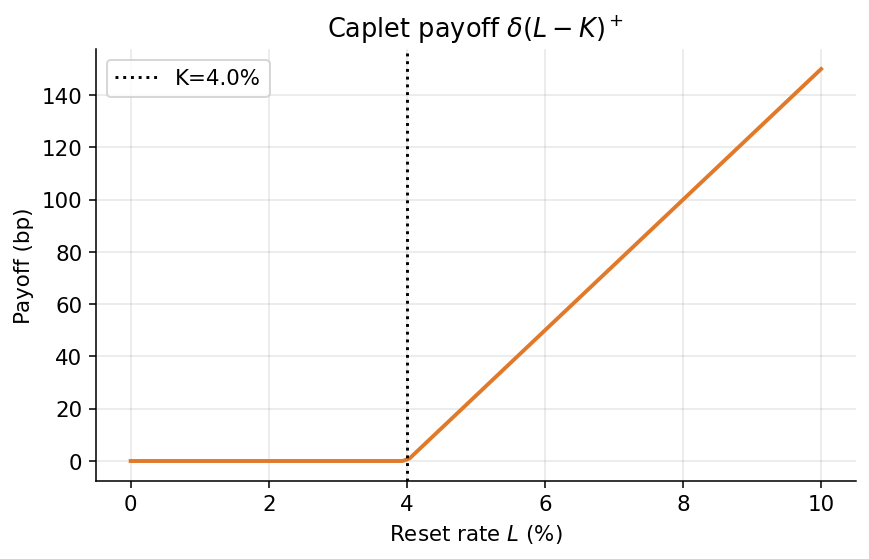
\includegraphics[keepaspectratio]{figures/ch14-caplet-payoff.png}}
\emph{Caplet payoff vs reset rate: hockey-stick in \(\ell\) --- zero
below the strike, slope \(\Delta t_k\) above. Convex in \(\ell\)
\(\Rightarrow\) the cap is long vega in the forward-rate vol.}

So the cap is a strip of caplets, each one a call option on the forward
LIBOR rate fixed at \(t_{k-1}\) and paid at \(t_k\). The hockey-stick
payoff above also reveals why a cap is convex in the rate: every caplet
is, and the sum of convex functions is convex. Convexity in the floating
rate translates directly into positive vega --- a cap always benefits
from a higher realized volatility of forward rates, holding everything
else fixed. This is the structural reason cap markets trade a vol
surface in the first place.

A brief note on naming. A ``1y1y'' caplet resets in one year and pays at
approximately one-year-and-one-tenor. A ``5y cap'' is a strip of caplets
running from the first reset out to five years. Swaption quotes use a
two-dimensional grid, expiry × tenor, e.g.~``2y5y'' is a 2-year option
to enter a 5-year swap. Once you internalize the tenor grid, all this
nomenclature becomes self-explanatory.

\begin{center}\rule{0.5\linewidth}{0.5pt}\end{center}

\section{14.2 Caplet Price under the Risk-Neutral
Measure}\label{caplet-price-under-the-risk-neutral-measure}

Our job is to price a caplet today, at time \(t\). There are two natural
candidates for the numeraire we use to discount the random future
payoff: the money-market account \(B_t\), which is universal and always
available, or the zero-coupon bond \(P_t(t_k)\) maturing on the payment
date, which is more bespoke but (as we will see) much cleaner. Let us
try the money-market account first, and see why it fails.

Let \(g_t^{(k)}\) denote the price at time \(t\) of a caplet maturing at
\(t_k\) (payment date). Under the risk-neutral measure \(\mathbb{Q}\)
with bank-account numeraire \(B_t = \exp\!\int_0^t r_s\,\mathrm{d}s\):

\[
\frac{g_t^{(k)}}{B_t}
\;=\;
\mathbb{E}^{\mathbb{Q}}_t\!\left[\,\frac{\Delta t_k\,\bigl(L_{t_{k-1}}(t_k) - K\bigr)_{+}}{B_{t_k}}\,\right].
\tag{14.4}
\]

This is awkward because \(B_{t_k}\) is random and correlated with
\(L_{t_{k-1}}(t_k)\). Remedy: use the \(t_k\)-bond as numeraire (the
T-forward measure from Chapter 5).

\begin{quote}
Intuition. \(B_{t_k}\) depends on the entire short-rate path from \(t\)
to \(t_k\), and high rates imply both a high LIBOR fixing \emph{and}
heavy discounting --- these two effects do not separate inside the
expectation. Switching to \(P_t(t_k)\) as numeraire effectively
``pre-pays'' the discount at time \(t\), so the only random thing left
inside the expectation is the payoff itself.
\end{quote}

\begin{center}\rule{0.5\linewidth}{0.5pt}\end{center}

\section{\texorpdfstring{14.3 Change of Numeraire --- the
\(T_i\)-Forward
Measure}{14.3 Change of Numeraire --- the T\_i-Forward Measure}}\label{change-of-numeraire-the-t_i-forward-measure}

Under the \(t_k\)-forward measure \(\mathbb{Q}^{t_k}\), whose numeraire
is \(P_t(t_k) = P(t, t_k)\) (see Chapter 5 for the general
density-process construction and Girsanov drift shift):

\[
\frac{g_t^{(k)}}{P_t(t_k)}
\;=\;
\mathbb{E}_t^{\mathbb{Q}^{t_k}}\!\left[\,\frac{\bigl(L_{t_{k-1}}(t_k) - K\bigr)_{+}}{P_{t_k}(t_k)}\,\right]\Delta t_k
\;=\;
\mathbb{E}_t^{\mathbb{Q}^{t_k}}\!\left[\bigl(L_{t_{k-1}}(t_k) - K\bigr)_{+}\right]\Delta t_k,
\tag{14.5}
\]

since \(P_{t_k}(t_k) = 1\). Read (14.5) carefully. The discount factor
\(1/B_{t_k}\) that plagued (14.4) has been replaced by
\(1/P_{t_k}(t_k) = 1\), because the \(t_k\)-bond is worth exactly one
dollar on its own maturity. All of the discounting has been absorbed
into the \(P_t(t_k)\) that sits outside the expectation. What is left
inside the expectation is just the clean payoff. This is the payoff of a
textbook call option on \(L_{t_{k-1}}(t_k)\), evaluated under the
measure \(\mathbb{Q}^{t_k}\), with no discount to worry about.

Plugging in (14.2),
\(L_{t_{k-1}}(t_k) = \tfrac{1}{\Delta t_k}\!\left[\tfrac{1}{P_{t_{k-1}}(t_k)} - 1\right]\).

Define the likelihood ratio (key ratio that becomes a martingale under
\(\mathbb{Q}^{t_k}\)):

\[
X_t \;=\; \frac{P_t(t_{k-1})}{P_t(t_k)}\,,
\qquad
X_{t_{k-1}} = \frac{1}{P_{t_{k-1}}(t_k)}.
\tag{14.6}
\]

\(X_t\) is a ratio of two tradable zero-coupon bonds, one of which is
the numeraire --- the generic template for a
\(\mathbb{Q}^{t_k}\)-martingale (Chapter 5).

\subsection{Vasicek illustration}\label{vasicek-illustration}

In the Vasicek model bond prices are affine (Chapter 12):

\[
P_t(T) \;=\; e^{\,A_t(T) \,-\, B_t(T)\,r_t},
\qquad
\frac{\mathrm{d}P_t(T)}{P_t(T)} \;=\; r_t\,\mathrm{d}t \,-\, B_t(T)\,\sigma\,\mathrm{d}\widetilde{W}_t,
\tag{14.7}
\]

with drift \(r_t\) and volatility \(B_t(T)\sigma\) --- larger for
longer-dated bonds.

Taking \(\mathrm{d}\ln\) of \(X_t\):

\[
\frac{\mathrm{d}X_t}{X_t}
\;=\;
\bigl(\operatorname{vol}\,t_{k-1} - \operatorname{vol}\,t_k\bigr)\,
\;=\;
\bigl(-B_t(t_{k-1}) + B_t(t_k)\bigr)\,\sigma\,\mathrm{d}\widetilde{W}_t^{(k)},
\tag{14.8}
\]

where \(\widetilde{W}_t^{(k)}\) is a Brownian motion under
\(\mathbb{Q}^{t_k}\). The drift has cancelled --- \(X_t\) is a
\(\mathbb{Q}^{t_k}\)-martingale, consistent with being a ratio of a
tradable (\(P_t(t_{k-1})\)) and the numeraire (\(P_t(t_k)\)). This
cancellation is not an accident of the Vasicek model; it is a general
fact about changes of numeraire (Chapter 5), of which Vasicek is just a
concrete instance.

Write the bond-vol differential as

\[
\Sigma_t \;\equiv\; -B_t(t_{k-1}) + B_t(t_k),
\qquad
\mathrm{d}\widetilde{W}_t^{(k)} = B_t(t_k)\,\sigma\,\mathrm{d}t + \mathrm{d}\widetilde{W}_t.
\tag{14.9}
\]

The second equation is the key change-of-measure statement: when you
switch the numeraire from the bank account \(B_t\) to the \(t_k\)-bond
\(P_t(t_k)\), the Brownian motion that drives everything gets a drift
\(B_t(t_k)\sigma\). This drift is exactly the bond's volatility, which
is exactly the amount by which the new numeraire differs from the old.
That is Girsanov talking (Chapter 5); the story is the same whatever the
driving model, as long as the numeraire is a strictly positive tradable.

Then

\[
g_t^{(k)} \;=\; P_t(t_k)\,\mathbb{E}_t^{\mathbb{Q}^{t_k}}\!\left[\,(X_{t_{k-1}} - \mathcal{K})_+\,\right]\Delta t_k,
\qquad \mathcal{K} \equiv 1 + \Delta t_k\,K.
\tag{14.10}
\]

Notice the strike transformation. In terms of LIBOR the strike was
\(K\); in terms of \(X = 1/P_{t_{k-1}}(t_k)\) it becomes
\(\mathcal{K} = 1 + \Delta t_k K\). This is just a re-expression of the
same kink in the payoff function; the kink sits at whatever value of the
underlying makes the pre-\((\cdot)_+\) expression vanish. Because \(X\)
and \(L\) are affinely related, an option on one is exactly an option on
the other, with a re-scaled strike and a re-scaled notional. No
information lost.

Because \(X_t\) is a log-normal \(\mathbb{Q}^{t_k}\)-martingale (in the
Gaussian Vasicek case), this is exactly a Black-Scholes expectation:

\[
\boxed{\;
g_t^{(k)}
\;=\;
P_t(t_k)\,\Bigl[\,X_t\,\Phi(d_+) - \mathcal{K}\,\Phi(d_-)\,\Bigr]
\;}
\tag{14.11}
\]

\[
d_{\pm}
\;=\;
\frac{\ln(X_t/\mathcal{K}) \;\pm\; \tfrac{1}{2}\int_t^{t_{k-1}}\Sigma_s^{\,2}\,\mathrm{d}s}
{\left(\int_t^{t_{k-1}}\Sigma_s^{\,2}\,\mathrm{d}s\right)^{1/2}}.
\tag{14.12}
\]

The term \(\int_t^{t_{k-1}}\Sigma_s^{\,2}\,\mathrm{d}s\) is the
cumulative quadratic variation of \(\ln X\) up to the fixing date. In a
stationary Black-76 framing it will simply become
\(\sigma^2(t_{k-1}-t)\) --- a single vol times time to fix --- but in a
more general model it can be time-dependent. Either way, the structure
is Black-Scholes: log-moneyness divided by a standard deviation.

\subsection{Cap as a sum of caplets}\label{cap-as-a-sum-of-caplets}

\[
\mathrm{Cap}_t \;=\; \sum_{k=1}^{n} g_t^{(k)}.
\tag{14.13}
\]

This single equation is the whole point of the change of numeraire. We
got here because the cap payoff is a \emph{sum} of single-date payoffs;
each single-date payoff depends on a fixing at a single date; and each
fixing can be priced under its \emph{own} forward measure. There is no
need for a joint model of the whole forward-rate curve --- you only need
one marginal distribution per fixing date. That is a huge reduction in
modelling burden, and it is the structural reason caps are vastly easier
to price than path-dependent products.

\begin{center}\rule{0.5\linewidth}{0.5pt}\end{center}

\subsection{Case study (a): UK LDI / mini-budget Sept 2022 --- pension
swaption book forced
unwind}\label{case-study-a-uk-ldi-mini-budget-sept-2022-pension-swaption-book-forced-unwind}

\emph{On 23 September 2022 the UK Chancellor Kwasi Kwarteng delivered a
``mini-budget'' of \(\pounds 45\)B in unfunded tax cuts. The \(30\)-year
gilt yield jumped from \(\approx 3.7\%\) to \(\approx 5.1\%\) over the
next five trading sessions --- a move that LDI (Liability-Driven
Investment) hedge books at UK defined-benefit pension schemes had
collectively calibrated as a \(7\sigma\)-plus tail. The Bank of England
intervened on \(28\) September with a \(\pounds 65\)B emergency
gilt-buying programme to break the resulting forced-seller doom-loop.}

\textbf{Context.} UK defined-benefit pension funds carry long-dated
nominal liabilities --- promises to pay specific amounts to retirees
over the next \(30\)--\(50\) years --- that have effective duration of
\(20\)--\(25\) years. The funded portion is typically invested in growth
assets (equities, credit, alternatives) with much shorter duration; the
resulting asset-liability duration mismatch is the dominant source of
funding-ratio volatility for the scheme. LDI is the post-\(2000\)s
solution: layer a leveraged interest-rate hedge on top of the existing
portfolio using long-dated receiver IRS plus receive-fixed swaptions to
take the asset-side duration up to match the liability side. Because the
IRS overlay is funded only by initial-margin posting against trustees'
collateral pool (typically gilts and cash), schemes can match
\(\pounds 1\)B of liability duration with
\(\pounds 100\)M--\(\pounds 250\)M of collateral. The market grew
enormously after the Pensions Act \(2004\) made funding-ratio reporting
mandatory; by mid-\(2022\) UK LDI mandates aggregated to
\(\sim \pounds 1.6\)T of notional swap exposure.

The mini-budget shock was not a typical rates move. The \(30\)y gilt
yield's \(140\) bp jump in five sessions implied a one-week realised vol
of \(\sim 28\%\) on \(30\)y rates, against an implied vol of \(\sim 90\)
bp/year (\(\approx 12.5\%\) on rate) used in standard LDI risk
frameworks --- that is approximately a \(7\)-standard-deviation move on
the calibrated normal distribution. The mark-to-market loss on the
receive-fixed legs was enormous: with portfolio dv\(01\) across the LDI
universe estimated at \(\pounds 200\)M--\(\pounds 300\)M per basis
point, the \(140\) bp move generated \(\pounds 30\)B+ of MTM losses,
against collateral pools of \(\sim 5\)--\(10\%\) of notional. Schemes
had to post variation margin within \(T+1\), which for many meant
selling gilts to raise cash. The forced gilt selling pushed yields even
higher, triggered more margin calls, and produced a self-reinforcing
doom-loop that the BoE's intervention was specifically designed to halt
--- buying long-dated gilts unconditionally for \(13\) trading days to
put a ceiling on yields and let LDI managers raise collateral in an
orderly fashion.

\textbf{Reading it through the chapter's math.} The receive-fixed
swaption book sits on the right side of (14.27): swaption value
\(X_t(S_t \Phi(d_+) - F\Phi(d_-))\) written here in payer-equivalent
form --- for the receivers actually held by LDI schemes, swap put-call
parity flips the sign, giving \(X_t(F\Phi(-d_-) - S_t\Phi(-d_+))\), so a
rate rise of \(140\) bp moves the book the other way (a loss for
receive-fixed). The Greeks: dv\(01\) on a \(30\)y receive-fixed IRS is
approximately the annuity \(X_t\), which for a \(30\)-year UK swap at
\(4\%\) fixed runs to \(\approx 17.5\) --- meaning a \(1\) bp parallel
shift moves the IRS PV by \(0.175\%\) of notional, or \(\pounds 1.75\)M
per \(\pounds 1\)B notional. Across the LDI universe of
\(\pounds 1.6\)T, dv\(01\) aggregates to \(\pounds 280\)M/bp --- and a
\(140\) bp move thus equals \(\pounds 39\)B of MTM loss in aggregate,
against industry-wide collateral pools of
\(\sim \pounds 80\)--\(\pounds 150\)B. Per scheme, the IR delta as a
fraction of capital ran \(10\%\)--\(20\%\) per \(100\) bp move --- a
Black-\(76\) dv\(01\) calculation that risk systems had been computing
correctly for years. The vega contribution from receive-fixed swaptions
added another \(5\)--\(8\%\) of capital per vol point, and the
\(30\)-year normal swaption vol roughly tripled (from \(\sim 90\) bp/y
to \(\sim 280\) bp/y at peak) over the week. None of this was novel
mathematics; what was novel was the \emph{speed} at which the move
unfolded.

\textbf{Lesson.} The LDI failure mode was \emph{liquidity}, not pricing:
the math of (14.27) said correctly how much collateral needed to be
posted; the math did not say that gilts could not be sold to raise the
collateral without crashing the gilt market itself in turn. In the
abstract, the strategy works --- long-dated rate hedges genuinely match
long-dated liability duration, and over a multi-decade horizon the
leverage cost is well-compensated by the liability-matching benefit. The
problem is the path: a sudden fiscal shock transmits into a margin call
into a fire-sale in \(48\) hours, and the dv\(01\)-based stress
framework that LDI managers used (typically a \(200\) bp instantaneous
shift with \(T+5\) remediation) was not calibrated to a \(T+1\)
collateral cycle in a market without unconditional buyers. Sovereign
rate vol breaking a hedge book is a recurring theme --- UK LDI \(2022\),
US Treasury basis trade \(2020\), Mexican peso \(1994\), Italian BTP
\(2018\), and the same pattern shows up in \(1998\) Long-Term Capital.
The deeper lesson for the new hire is that a hedge book's leverage limit
should be set by \emph{liquidity-adjusted} collateral availability under
stress, not by mark-to-market \(99\%\) VaR on a \(5\)-year history, and
that central-bank backstop optionality is now an implicit hedge in every
long-duration rates book --- when the BoE intervened on \(28\)
September, \(30\)y vols collapsed \(30\%\) in a single session,
vindicating the underlying Black machinery once the regime stabilised
but only after \(\pounds 1.6\)T of liability-hedge exposure had been
threatened by a five-day fiscal shock.

\begin{center}\rule{0.5\linewidth}{0.5pt}\end{center}

\section{14.4 Black Implied Vols --- the Market
Convention}\label{black-implied-vols-the-market-convention}

The Vasicek derivation gave us a Black-style formula, but the market
standard is to skip the short-rate model and assume directly that each
forward LIBOR is log-normal under its own \(t_k\)-forward measure (GBM
for forward rates). This is the LIBOR market model (LMM / BGM) seed.

Let
\(L_{t_{k-1}}(t_k) \stackrel{d}{=} L_t(t_{k-1}, t_k) \cdot Y_{t_{k-1}}\),
where \(L_t(t_{k-1}, t_k)\) is today's forward rate for the
\([t_{k-1}, t_k]\) period:

\[
L_t(t_{k-1}, t_k)
\;=\;
\frac{1}{\Delta t_k}\!\left[\frac{P_t(t_{k-1})}{P_t(t_k)} - 1\right].
\tag{14.14}
\]

Using
\(P_t(t_{k-1}) = P_t(t_k)\bigl(1 + \Delta t_k L_t(t_{k-1}, t_k)\bigr)\),
\(L_t(t_{k-1}, t_k)\) is a ratio of tradables to the numeraire
\(P_t(t_k)\), hence a \(\mathbb{Q}^{t_k}\)-martingale.

\pandocbounded{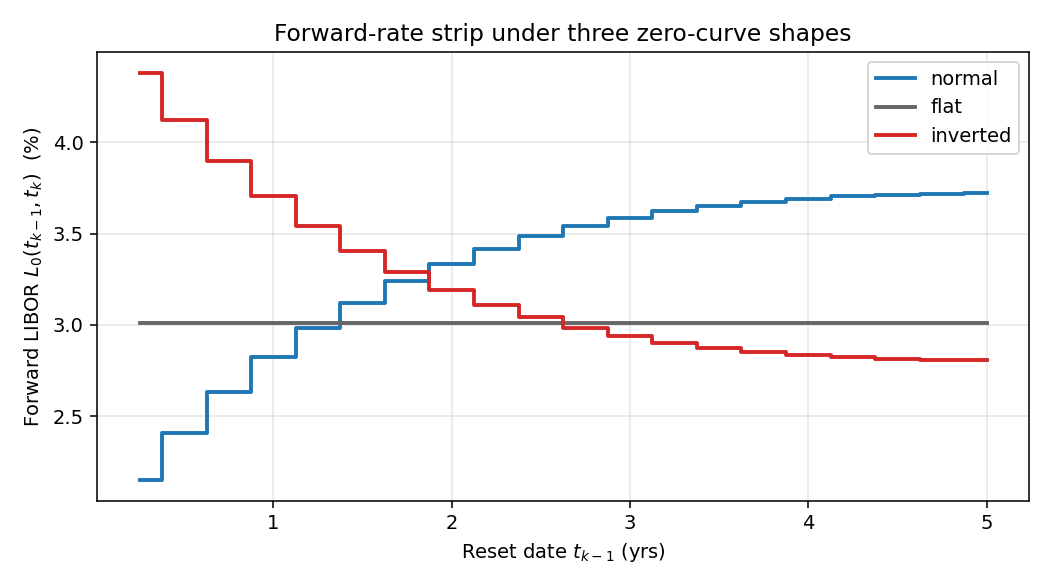
\includegraphics[keepaspectratio]{figures/ch14-forward-strip-shapes.png}}
\emph{Normal (upward-sloping), flat, and inverted zero-curves imply very
different forward-LIBOR strips \(\{L_0(t_{k-1},t_k)\}_k\).}

Postulate driftless GBM under that measure:

\[
\frac{\mathrm{d}L_t^{(k)}}{L_t^{(k)}} \;=\; \sigma\,\mathrm{d}W_t^{t_k},
\qquad L_t^{(k)} \equiv L_t(t_{k-1}, t_k).
\tag{14.15}
\]

``\(\mathbb{Q}\)-Brownian motion'' here means under
\(\mathbb{Q}^{t_k}\). This is the direct postulate: forward LIBOR is a
log-normal martingale under its own forward measure. The only free
parameter is the volatility \(\sigma\); by assumption the drift is zero
(which is forced, because \(L^{(k)}\) is a martingale under
\(\mathbb{Q}^{t_k}\)). There is nothing to solve --- given \(\sigma\),
the distribution of \(L_{t_{k-1}}^{(k)}\) is pinned down.

Starting at \(t\):

\[
L_{t_{k-1}}^{(k)} \;=\; L_t(t_{k-1}, t_k)\,\exp\!\Bigl(-\tfrac{1}{2}\sigma^2(t_{k-1}-t) \,+\, \sigma\bigl(W_{t_{k-1}}^{t_k} - W_t^{t_k}\bigr)\Bigr).
\tag{14.16}
\]

This is the textbook GBM solution: log-mean
\(-\tfrac12\sigma^2(t_{k-1}-t)\), log-variance \(\sigma^2(t_{k-1}-t)\),
multiplicative shift by the forward rate today. The log-normality is
what keeps forward LIBOR strictly positive --- a feature that made
perfect sense in the regime before the 2008 financial crisis, and that
causes trouble afterwards (see §14.4b below).

\subsection{Black's formula for a
caplet}\label{blacks-formula-for-a-caplet}

Plug (14.16) into (14.5). Since \(L_{t_{k-1}}^{(k)}\) is log-normal with
mean \(L_t^{(k)}\) under \(\mathbb{Q}^{t_k}\):

\[
g_t^{(k)} \;=\; P_t(t_k)\,\mathbb{E}^{\mathbb{Q}^{t_k}}\!\left[\,\bigl(L_{t_{k-1}}^{(k)} - K\bigr)_+\,\right]\Delta t_k,
\]

\[
\boxed{\;
g_t^{B(k)}
\;=\;
P_t(t_k)\,\Bigl\{\,L_t(t_{k-1}, t_k)\,\Phi(d_+) \;-\; K\,\Phi(d_-)\,\Bigr\}\,\Delta t_k
\;}
\tag{14.17}
\]

\[
d_{\pm}
\;=\;
\frac{\ln\!\bigl(L_t(t_{k-1}, t_k)/K\bigr) \;\pm\; \tfrac{1}{2}\sigma^2(t_{k-1} - t)}
{\sigma\,(t_{k-1} - t)^{1/2}}.
\tag{14.18}
\]

This is the Black-76 caplet formula. Each caplet has its own vol
\(\sigma_k^{B\ell}\) (the ``Black caplet vol''). Structurally, (14.17)
is Black-Scholes on spot \(L_t\), strike \(K\), vol \(\sigma\), expiry
\(t_{k-1}-t\), with the discount \(P_t(t_k)\) taking the payment date
--- the forward-measure dislocation between fix at \(t_{k-1}\) and pay
at \(t_k\).

\textbf{Cross-reference.} The same caplet can be re-expressed as a put
on a \(t_k\)-zero-coupon bond with strike
\(K_{\text{bond}} = 1/(1 + K\Delta t_k)\); see Chapter 13 §13.6 for the
Vasicek-Black bond-put formula that provides an equivalent (and useful)
consistency check.

\pandocbounded{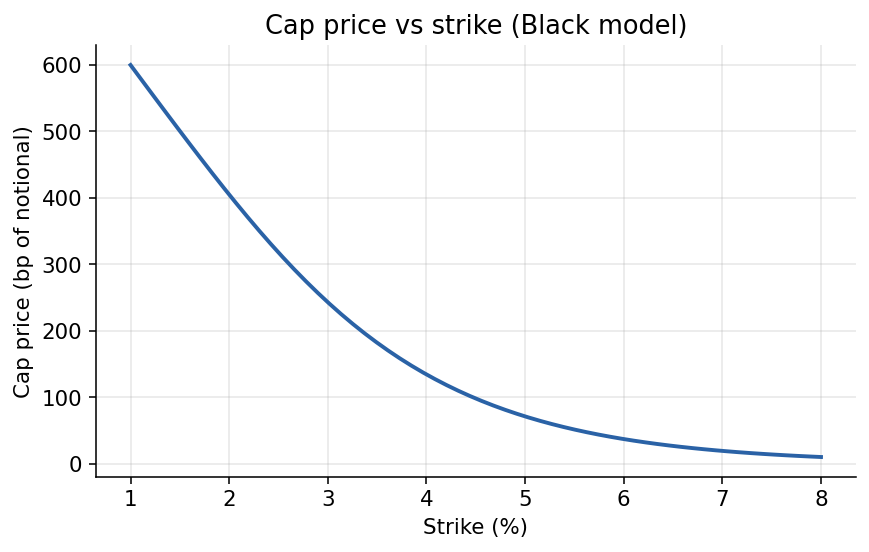
\includegraphics[keepaspectratio]{figures/ch14-cap-price.png}}
\emph{Cap price vs strike (Black model)}

The cap price is monotonically decreasing in the strike \(K\) (higher
strike, less in-the-money, less intrinsic, less option value). For very
low strikes the cap behaves like a forward swap (all caplets deep in the
money, optionality worth almost nothing on top of intrinsic). For very
high strikes the cap behaves like a lottery ticket (all caplets deep out
of the money, value almost entirely time value). The curvature between
these extremes is driven by the Black caplet vol term structure; that is
what makes the cap surface genuinely interesting.

\subsection{Cap in terms of Black
vols}\label{cap-in-terms-of-black-vols}

\[
\sum_{k=1}^{n} g_t^{B(k)} \;=\; \sum_{k=1}^{n} g_t^{B(k)}(\sigma_k^{B\ell}),
\tag{14.19}
\]

with \(\sigma_k^{B\ell}\) the k-th caplet Black implied vol.~A flat cap
vol \(\sigma_n^{C\ell}\) is the single \(\sigma\) such that
\(\sum_k g^B(\sigma) = \mathrm{Cap}_t^{\mathrm{mkt}}\) --- conceptually
useful but coarser than the per-caplet term structure.

One ``strips'' caplet vols recursively from quoted cap prices: each cap
tenor introduces one new unknown vol, solved one at a time so every
market-quoted cap reprices exactly. The market quotes at several
strikes; stripping is done at each strike, giving a 2D caplet-vol
surface in (expiry, strike), through which traders typically fit a SABR
smile per expiry.

\pandocbounded{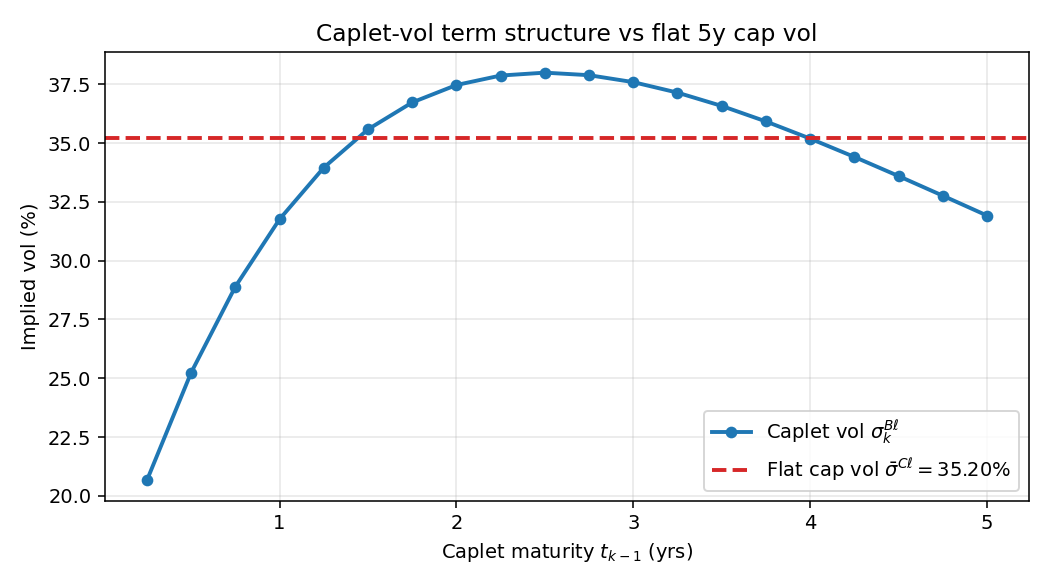
\includegraphics[keepaspectratio]{figures/ch14-caplet-vol-ts.png}}
\emph{A stylized humped caplet-vol curve \(\sigma_k^{B\ell}\) alongside
the flat cap vol \(\bar\sigma^{C\ell}\) that reprices the whole 5y cap.}

\begin{quote}
Why cap \(=\) sum of caplets exactly (no cross-terms). Each caplet pays
\(\Delta t_k(L_{t_{k-1}}(t_k)-K)_+\) on a \emph{single} fixed date
\(t_k\). The cap payoff is the pointwise sum and expectation is linear,
so \(\text{Cap}_t = \sum_k g_t^{(k)}\) --- no covariance terms. Each
caplet prices under its \emph{own} forward measure with its \emph{own}
Black vol.~A swaption, by contrast, takes a max on the
\emph{already-summed} swap value, forcing a different numeraire (the
annuity) and bringing in forward-rate correlations.
\end{quote}

\begin{center}\rule{0.5\linewidth}{0.5pt}\end{center}

\section{14.4b Bachelier vs Black in a Negative-Rate
World}\label{b-bachelier-vs-black-in-a-negative-rate-world}

The Black-76 framework above rests on one assumption that is
uncontroversial in most of modern financial history: that forward rates
are strictly positive. Log-normality forces this, since
\(L_{t_{k-1}}^{(k)} = L_t^{(k)} \exp(\text{something})\) and the
exponent is always strictly positive. For decades this was a reasonable
view of the world --- a negative short rate was almost unthinkable,
because banks could always hold physical cash instead of lending at a
loss, and so the zero lower bound seemed binding by arbitrage.

The post-2008 experience blew that up. The European Central Bank, the
Swiss National Bank, the Bank of Japan, and others spent multiple years
with deposit rates set explicitly below zero, and market forward rates
on EURIBOR and JPY curves traded visibly negative across a wide range of
tenors. Suddenly Black-76 could not even \emph{represent} a market quote
--- you cannot compute \(\ln(L/K)\) if \(L\) is negative, and the model
assigns zero probability to outcomes that were happening in real time.

Market practice migrated in two directions. The first was the
\emph{shifted-Black} model: write \(L \to L + \alpha\) for some positive
shift \(\alpha\), assume that \(L + \alpha\) is log-normal under
\(\mathbb{Q}^{t_k}\), and price Black-76 with the shifted variables.
This is a cheap fix --- it preserves the closed-form and the market
intuition of a Black vol, while permitting negative realizations of
\(L\) itself as long as they stay above \(-\alpha\).

The second, more structural fix was the \emph{Bachelier} or
\emph{normal} model: assume that the forward rate follows arithmetic
Brownian motion rather than geometric, so

\[
\mathrm{d}L_t^{(k)} \;=\; \sigma_N\,\mathrm{d}W_t^{t_k},
\]

with \(\sigma_N\) the \emph{normal} (basis-point) volatility. The caplet
price under Bachelier is another closed-form expression involving
\(\Phi\) and the normal density, with a moneyness
\((L_t - K)/(\sigma_N \sqrt{t_{k-1}-t})\). The normal model prices
forward rates as a Gaussian distribution centered on the current
forward, with no lower bound --- perfectly happy to assign positive
probability to negative rates, because that is exactly what happened in
reality.

The two conventions are related by a rough rule of thumb: at the money,
\(\sigma_N \approx \sigma_B \cdot L\), where \(\sigma_B\) is the Black
vol and \(L\) is the underlying forward rate. So a 25\% Black vol on a
4\% forward is roughly equivalent to a 100 bp normal vol.~Away from ATM
they diverge, and the choice of quoting convention matters. Modern
rate-derivative desks now routinely switch between conventions, with
normal vols dominating European markets (especially EUR and CHF) and
shifted-Black or straight Black vols still common in USD markets where
the zero bound has remained in force for most of history.

The same observations apply to swaptions --- normal swaption vols are
now the industry standard in much of Europe, and a senior quant cannot
afford to be sloppy about which convention a given quote is in.

\begin{center}\rule{0.5\linewidth}{0.5pt}\end{center}

\section{14.5 Swaption as Black on the Swap
Rate}\label{swaption-as-black-on-the-swap-rate}

So far we have priced an option on a \emph{single} fixing of a forward
rate. A swaption is an option on an entire \emph{swap} --- a bundled set
of fixings. Crucially, the max is taken at the swap level, not at the
caplet level, so the cap's per-fixing decomposition no longer applies.
The right tool is a portfolio numeraire --- the annuity --- under which
the par swap rate becomes a single scalar martingale and the pricing
collapses to a one-dimensional Black call.

A swaption (swap option) gives A the right, at \(t_0\), to enter a payer
swap with fixed leg \(F\), reset/payment dates \(t_1, \dots, t_n\). The
payoff at exercise is

\[
C_{t_0} \;=\; \bigl(V_{t_0}^{\,\ell} - V_{t_0}^{\text{fixed}}\bigr)_{+},
\qquad
V_{t_0}^{\text{fixed}} \;=\; F\sum_{k=1}^{n} P_{t_0}(t_k)\,\Delta t_k,
\qquad
V_{t_0}^{\,\ell} \;=\; 1 - P_{t_0}(t_n).
\tag{14.20}
\]

(The floating-leg par identity \(V^\ell = 1 - P_{t_0}(t_n)\) comes from
Chapter 13.) Hence

\[
C_{t_0} \;=\; \Bigl(\,1 - P_{t_0}(t_n) \;-\; F\sum_{k=1}^{n} P_{t_0}(t_k)\,\Delta t_k\,\Bigr)_{+}.
\tag{14.21}
\]

The max operates on a nonlinear combination of \(n+1\) bond prices;
under a multi-factor model the max cannot be decomposed caplet-style.
The remedy is to choose a numeraire that matches the \emph{structure} of
the payoff --- the annuity.

\subsection{Annuity-measure swaption}\label{annuity-measure-swaption}

Collect terms using the annuity numeraire:

\[
X_t \;\equiv\; \sum_k \Delta t_k\,P_t(t_k) \quad\text{(annuity)}.
\tag{14.22}
\]

The annuity is a strictly positive portfolio of zero-coupon bonds ---
exactly the PV of \$1 received on every fixed-leg payment date --- so it
qualifies as a numeraire (Chapter 5). Change to \(\mathbb{Q}^{X}\) with
numeraire \(X_t\):

\[
\frac{g_t}{X_t}
\;=\;
\mathbb{E}^{\mathbb{Q}^{X}}_t\!\left[\,\left(\,\frac{1 - P_{t_0}(t_n)}{\sum_k \Delta t_k P_{t_0}(t_k)} \,-\, F\right)_{+}\,\right]
\;=\;
\mathbb{E}^{\mathbb{Q}^{X}}_t\!\bigl[(S_{t_0} - F)_{+}\bigr],
\tag{14.23}
\]

where the par swap rate is (recall Chapter 13's IRS section)

\[
\boxed{\;
S_t \;=\; \frac{1 - P_t(t_n)}{\sum_k \Delta t_k\,P_t(t_k)}
\;}
\tag{14.24}
\]

--- and \(S_t\) is a \(\mathbb{Q}^{X}\)-martingale (a ratio of the
tradable \(1 - P_t(t_n)\) to the numeraire \(X_t\)). Hence

\[
g_t \;=\; X_t\,\mathbb{E}^{\mathbb{Q}^{X}}_t\!\bigl[(S_{t_0} - F)_{+}\bigr].
\tag{14.25}
\]

All of the \(n\)-dimensional bond-price structure has collapsed into a
scalar call on the single random variable \(S_{t_0}\).

\subsection{Log-normal swap-rate model
(LSM)}\label{log-normal-swap-rate-model-lsm}

Assume

\[
\frac{\mathrm{d}S_t}{S_t} \;=\; \sigma\,\mathrm{d}\widetilde{W}_t^{X}
\;\Longrightarrow\; \text{Black formula for swaption.}
\tag{14.26}
\]

Then (under GBM with mean \(S_t\)):

\[
\boxed{\;
g_t \;=\; X_t\,\bigl(\,S_t\,\Phi(d_+) \;-\; F\,\Phi(d_-)\,\bigr)
\;}
\tag{14.27}
\]

\[
d_{\pm} \;=\; \frac{\ln(S_t/F) \;\pm\; \tfrac{1}{2}\sigma^{2}(t_0 - t)}{\sigma\,(t_0 - t)^{1/2}}.
\tag{14.28}
\]

This is the Black swaption formula: a call on the swap rate \(S_t\),
with the annuity \(X_t\) as discount factor. Same structure as
Black-Scholes on equity and as the Black caplet, with the right
numeraire (\(X_t\)) replacing the bank account or the single
\(t_k\)-bond.

\pandocbounded{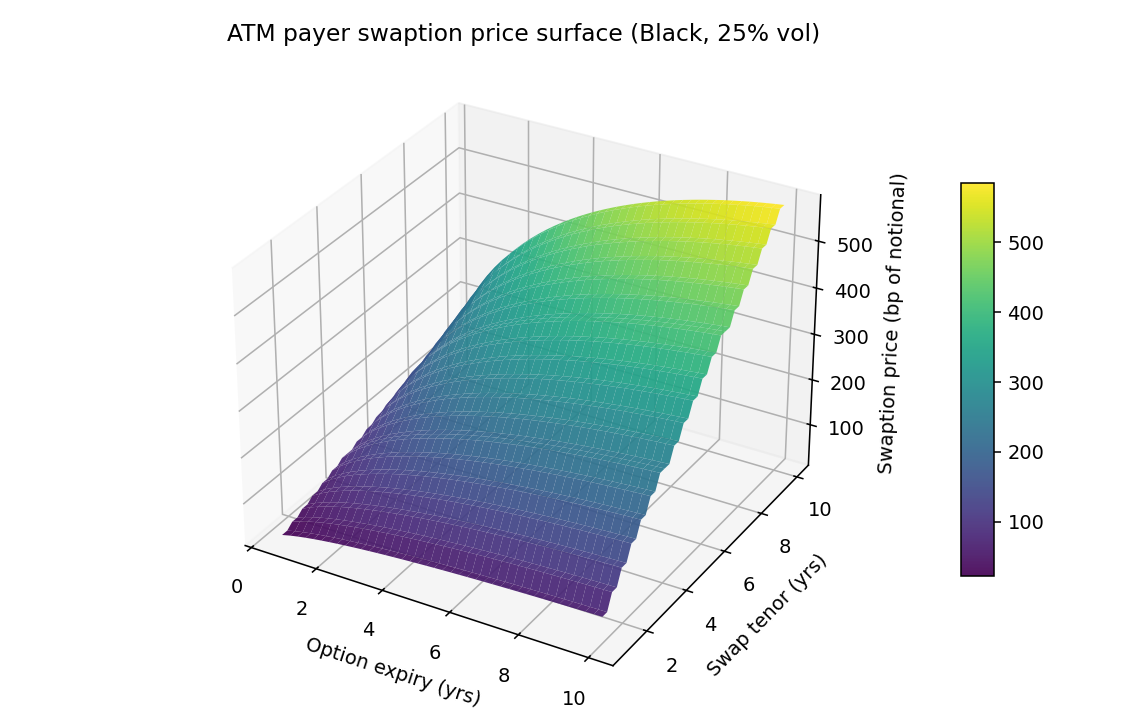
\includegraphics[keepaspectratio]{figures/ch14-swaption-surface.png}}
\emph{The Black swaption price varies smoothly over the expiry × tenor
grid --- the standard market quoting convention.}

The swaption market trades a \emph{two-dimensional} vol surface: expiry
× tenor. A 2y5y swaption is the 2-year option to enter a 5-year swap.
Consistency between the caplet surface (marginals) and the swaption
surface (functionals of the joint) is a nontrivial constraint that full
production models (LMM, SABR-LMM, stochastic-vol variants) try to fit
simultaneously.

\subsection{Historical alternative --- Jamshidian on a one-factor affine
model}\label{historical-alternative-jamshidian-on-a-one-factor-affine-model}

Before the annuity measure became the industry standard, swaptions were
priced by an exact decomposition that works in any one-factor Gaussian
short-rate model (Vasicek, Hull-White): because
\(\sum_k c_k P_{t_0}(t_k)\) is monotone in \(r_{t_0}\), the exercise
region \(\{r_{t_0} > r^*\}\) is a half-line, with \(r^*\) solving

\[
\sum_{k=1}^{n} c_k\,P_{t_0}(t_k; r^{*}) \;=\; 1,
\qquad c_k = F\,\Delta t_k\;(k<n),\;\; c_n = 1 + \Delta t_n F.
\tag{14.29}
\]

A joint indicator on all \(n\) bond prices reduces to a single scalar
condition on \(r_{t_0}\), and each bond-price term becomes a Gaussian
tail probability under \(\mathbb{Q}^{t_k}\). The full derivation is the
European bond-option machinery of Chapter 13 §13.7.4 --- we cite it
rather than re-derive. The route is pedagogically clean and historically
important, but the annuity-measure formula (14.27) is the production
form: it gives a one-shot Black on the par swap rate, requires no
calibrated short-rate model, and is the basis of every Bloomberg /
market quote for swaption vol.

\begin{center}\rule{0.5\linewidth}{0.5pt}\end{center}

\subsection{Case study (b): LIBOR → SOFR transition June
2023}\label{case-study-b-libor-sofr-transition-june-2023}

\emph{USD LIBOR formally ceased publication on \(30\) June \(2023\) for
the remaining tenors (\(1\)M, \(3\)M, \(6\)M, \(12\)M); the other major
settings (\(1\)W, \(2\)M) had ceased on \(31\) December \(2021\). At the
cessation date, an estimated \(\$200\)T+ of derivatives outstanding
referenced USD LIBOR --- IRS, caps, floors, swaptions, FRAs, structured
notes --- and every single contract had to be either re-papered to a
SOFR-based reference or fall back automatically under the ISDA \(2020\)
IBOR Fallbacks Protocol. ISDA estimates approximately \(85\%\) of
bilateral swap volume re-papered ahead of cessation; the remainder fell
back automatically. The largest contract-rewrite event in derivatives
history.}

\textbf{Context.} The LIBOR-replacement project began formally with the
Financial Stability Board's \(2014\) recommendations after the \(2012\)
rate-rigging scandals, but the operational mechanics of the swap-market
migration crystallised only in \(2017\)--\(2020\). The replacement rate
selected by the US Alternative Reference Rates Committee (ARRC) was the
Secured Overnight Financing Rate (SOFR) --- a
Treasury-repo-collateralised overnight rate published by the New York
Fed since April \(2018\). SOFR differs from LIBOR in two structural
ways: it is overnight-only (no term structure intrinsically; term SOFR
for select tenors is published as a forward-looking median of
SOFR-futures), and it is essentially risk-free (collateralised by
Treasuries, with a credit spread of zero versus LIBOR's \(\sim 25\) bp
average bank-credit spread). The ISDA \(2020\) Fallbacks Protocol,
opted-in by approximately \(14{,}500\) legal entities globally, defined
the precise mechanic: at cessation date, any USD-LIBOR fixing in a
covered contract is replaced by ``SOFR compounded in arrears over the
corresponding accrual period'' plus a \emph{fixed} spread adjustment.

The spread adjustment is the operationally critical detail: it is set at
the historical median of the LIBOR-versus-compounded-SOFR basis observed
over the five-year window prior to the announcement of cessation (March
\(2021\) for USD), and once set, \emph{frozen forever} for fallback
purposes. The published values are: \(11.448\) bp for \(1\)M USD LIBOR,
\(26.161\) bp for \(3\)M USD LIBOR, \(42.826\) bp for \(6\)M USD LIBOR,
and \(71.513\) bp for \(12\)M USD LIBOR. So a legacy \(5\)y IRS that
paid \(3\)M USD LIBOR + \(50\) bp now pays ``\(3\)M compounded SOFR +
\(26.161\) bp + \(50\) bp'' --- a frozen \(26.16\) bp uplift to the
spread, applied in perpetuity. The pricing impact at cessation was
largely zero by construction (the spread was set so that PV-neutrality
held in expectation under the prior basis); the operational impact was
enormous (every cap, floor, swaption, and structured note had to have
its payoff function rewritten).

\textbf{Reading it through the chapter's math.} Under LIBOR, a caplet
payoff is \(\Delta_k(L_{t_{k-1}}(t_{k-1}, t_k) - K)^+\) with the LIBOR
fixing \(L\) observed \emph{in advance} at \(t_{k-1}\) and the payment
made \emph{at} \(t_k\) --- exactly the (14.5) setup. The Black-\(76\)
formula \(C = \Delta_k P_t(t_k)[L_t \Phi(d_+) - K\Phi(d_-)]\) falls out
under log-normal forward-LIBOR dynamics because \(L_t\) is a
\(\mathbb{Q}^{t_k}\)-martingale (it is a ratio of tradable bond
differences to the \(P(t_k)\)-numeraire). Under SOFR, the fixing is
computed as
\(S_{t_{k-1}, t_k} = (1/\Delta_k)[\prod_{i}(1 + \Delta_i s_i) - 1]\)
where the product is over the daily SOFR fixings \(s_i\) within the
accrual period --- so the fixing is \emph{backward-looking} and known
only at \(t_k\), not at \(t_{k-1}\). Strictly speaking, this breaks the
(14.5) setup: the payoff is \(\Delta_k(S_{t_{k-1}, t_k} - K)^+\) paid at
\(t_k\), but \(S\) is now an in-arrears compound, not a forward fixing.
In practice, market dealers price the SOFR caplet in a
Black-\(76\)-shaped formula by treating the \emph{effective} fixing date
as a dealer-convention adjustment to the option's expiry (typically
taking the volatility integrand to run to a midpoint of the accrual
period, with a small lookback adjustment for the in-arrears effect). The
convexity correction between the in-advance fixing convention and the
in-arrears realisation is an order \(\sigma^2 \Delta_k\) term ---
typically \(0.1\)--\(0.5\) bp on a quarterly accrual at \(1\%\) vol.~For
a swaption on the SOFR-OIS swap, the par-swap-rate \(S_t\) is again a
\(\mathbb{Q}^{\mathrm{ann}}\)-martingale (the annuity numeraire
structure is unchanged); the Black-\(76\) formula (14.27) applies to
compounded-SOFR par swap rates exactly as it did to LIBOR-IRS par swap
rates, because nothing in the derivation depended on the compounding
convention of the floating leg.

\textbf{Lesson.} The cessation event was the largest stress test of
derivatives infrastructure in history: every cap, floor, swaption, IRS,
FRA, and structured note had to be re-papered or fall back, and every
risk system, settlement system, and accounting system had to be updated
to handle the new index. That the global market migrated \(\$200\)T+ of
notional across a single weekend (the \(30\) June \(2023\) cessation,
with the post-cessation Monday opening on the new convention) without
major operational failure is a quiet triumph of the multi-year ISDA-led
preparation. The deeper lesson for the new hire is that the Black-\(76\)
pricing architecture survived intact --- what changed was the index, the
fixing convention (forward-looking \(\to\) backward-looking), and the
spread-adjustment mechanic. Every formula in this chapter ports to SOFR
with \(L_t \to\) compounded-SOFR-forward and a small in-arrears
convexity adjustment; nothing about the change-of-numeraire derivation,
the annuity-measure pricing, or the per-caplet implied-vol convention
required revision. Risk systems that had abstracted ``LIBOR'' to ``the
simple forward rate under its own forward measure'' survived the
transition with minor wiring changes; risk systems that hardcoded
``LIBOR'' as a literal index name had to be substantially rewritten.
Index-agnostic abstractions are not academic luxury --- they are the
difference between a six-month transition project and a three-year one.

\begin{center}\rule{0.5\linewidth}{0.5pt}\end{center}

\section{14.6 Worked Example --- Pricing a 1-into-3m
Caplet}\label{worked-example-pricing-a-1-into-3m-caplet}

Concrete numbers are the best way to anchor the formulas. Let us price a
single quarterly caplet using the Black-76 formula and check that the
answer makes sense.

Suppose today is \(t = 0\), with:

\begin{itemize}
\tightlist
\item
  \(t_{k-1} = 1\) yr, \(t_k = 1.25\) yr, \(\Delta t_k = 0.25\) yr.
\item
  Today's forward rate \(L_0(1, 1.25) = 4.00\%\).
\item
  Strike \(K = 3.50\%\).
\item
  Black caplet vol \(\sigma = 25\%\).
\item
  Discount \(P_0(1.25) = 0.955\).
\end{itemize}

The caplet is forward-ITM with 1y to fix at 25\% vol --- meaningful time
value.

Compute:

\[
d_+ = \frac{\ln(0.04/0.035) + 0.5(0.25)^{2}(1)}{0.25\sqrt{1}}
 = \frac{0.1335 + 0.03125}{0.25}
 = 0.659,
\] \[
d_- = d_+ - 0.25 = 0.409.
\]

With \(\Phi(0.659) \approx 0.745\), \(\Phi(0.409) \approx 0.659\):

\[
g_0 = 0.955 \times \bigl(0.04 \times 0.745 - 0.035 \times 0.659\bigr)\times 0.25
\] \[
 = 0.955 \times (0.02980 - 0.02307)\times 0.25
 = 0.955 \times 0.006734 \times 0.25
 \approx 0.001607
\]

i.e.~about 16.07 bp of notional --- the caplet PV. Rough intrinsic:
\(0.25 \times (0.04 - 0.035) \times 0.955 \approx 11.94\) bp; the Black
price is \textasciitilde4 bp above intrinsic --- the time-value
contribution.

\pandocbounded{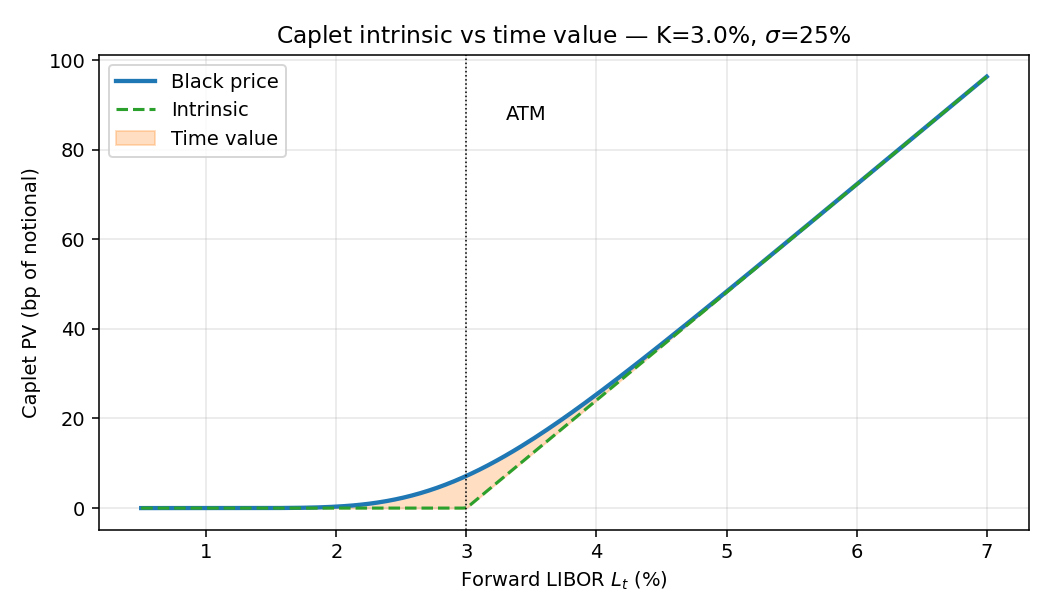
\includegraphics[keepaspectratio]{figures/ch14-caplet-decomp.png}}
\emph{For a 1y caplet, the Black price splits into intrinsic
\(P_t(t_k)\Delta t_k(L_t-K)_+\) and time value
\(g_t^{B(k)}-\text{intrinsic}\). The time component peaks near ATM and
decays symmetrically in \(\ln(L/K)\) --- the classic log-moneyness
curvature that drives cap vega.}

\section{14.7 Worked Example --- Stripping Caplet Vols from a 2-Year
Cap}\label{worked-example-stripping-caplet-vols-from-a-2-year-cap}

A harder and more realistic task is to back out caplet vols from market
cap quotes. Assume we see market prices for quarterly-settled caps at
two tenors, and we want to produce a caplet-vol term structure
consistent with both. The mechanics of the stripping procedure are easy
once you see them laid out.

Suppose quarterly caps:

\begin{itemize}
\tightlist
\item
  1-yr cap (4 caplets) trades at \(C_4^{\mathrm{mkt}}\).
\item
  2-yr cap (8 caplets) trades at \(C_8^{\mathrm{mkt}}\).
\end{itemize}

Given already-stripped \(\{\sigma_1^{B\ell}, \dots, \sigma_4^{B\ell}\}\)
from the 1-yr cap, solve

\[
C_8^{\mathrm{mkt}} - \sum_{k=1}^{4} g^{B(k)}\bigl(\sigma_k^{B\ell}\bigr)
\;=\;
\sum_{k=5}^{8} g^{B(k)}(\sigma^{\star})
\]

for the common forward caplet vol \(\sigma^{\star}\) over caplets 5--8
(1D root find). Repeating at longer tenors builds the full caplet-vol
term structure. In practice caps are quoted at multiple strikes;
stripping is done per strike, fit through with SABR smile to give a 2D
arbitrage-free surface.

\begin{center}\rule{0.5\linewidth}{0.5pt}\end{center}

\section{14.8 LIBOR to SOFR and the Index-Agnostic Black
Framework}\label{libor-to-sofr-and-the-index-agnostic-black-framework}

Case study (b) above walked the operational arc of the June 2023
USD-LIBOR cessation; this section states the structural takeaway
separately. The Black-76 caplet/swaption framework derived in
§14.1--§14.5 never depended on LIBOR specifically --- it depended only
on the existence of a \emph{simple forward rate} that is a martingale
under its own \(T_i\)-forward (or annuity) measure. The post-LIBOR
overnight-RFR world --- SOFR, SONIA, €STR, TONA, SARON --- replaces the
forward LIBOR fixing with a \emph{compounded in-arrears} fixing computed
over the accrual period, plus, for legacy contracts, a frozen ISDA
spread adjustment (11.448, 26.161, 42.826, 71.513 bp for 1M/3M/6M/12M
USD).

Three structural consequences for the framework. First, the
simple-forward identity (14.2) becomes an in-arrears compound ---
backward-looking rather than forward-looking, so the fixing is known
only at the end of the accrual period. Second, the resulting
in-arrears-vs-in-advance convexity carries a small but nonzero
order-\(\sigma^2 \Delta_k\) adjustment (\(0.1\)--\(0.5\) bp on quarterly
accruals at \(1\%\) vol). Third, the annuity-measure derivation of
(14.27) for swaptions is \emph{unchanged}: the par swap rate is still an
annuity-numeraire martingale regardless of whether the floating leg
compounds daily SOFR or fixes 3M LIBOR. Risk systems that abstracted
``LIBOR'' to ``simple forward rate under its own forward measure''
survived the transition with wiring changes; systems that hardcoded
``LIBOR'' needed substantial rewrites.

\section{14.9 Key Takeaways}\label{key-takeaways-13}

\begin{enumerate}
\def\labelenumi{\arabic{enumi}.}
\tightlist
\item
  Cap = strip of caplets. Each caplet is a European call on a forward
  LIBOR rate, fixed at \(t_{k-1}\) and paid at \(t_k\). The ``cap = sum
  of caplets'' decomposition is exact (no cross-terms), because the max
  acts on each caplet's fixing separately.
\item
  Pricing numeraire: switching from \(B_t\) to \(P_t(t_k)\) kills the
  correlation between discount and payoff. Under \(\mathbb{Q}^{t_k}\)
  the forward LIBOR \(L_t(t_{k-1}, t_k)\) is a martingale, because it is
  a ratio of the tradable \((P_t(t_{k-1}) - P_t(t_k))/\Delta t_k\) to
  the numeraire \(P_t(t_k)\).
\item
  Change of measure (Chapter 5):
  \(\mathrm{d}\widetilde{W}_t^{(k)} = B_t(t_k)\sigma\,\mathrm{d}t + \mathrm{d}\widetilde{W}_t\)
  in the Vasicek model of Chapter 12; more generally, drift compensation
  absorbs the bond-vol.~This is just Girsanov applied to the
  \(P_t(t_k)\)-numeraire.
\item
  Black-76 caplet falls out when we postulate log-normal forward rates
  under \(\mathbb{Q}^{t_k}\) --- one implied vol per caplet, not one per
  cap. Quoting flat cap vols is a convenience; hedging is always in
  terms of the per-caplet term structure.
\item
  In negative-rate regimes, Black-76 fails outright because \(\ln L\) is
  undefined. Shifted-Black and Bachelier models are the two practical
  fixes; normal (Bachelier) vols dominate European quoting conventions
  today.
\item
  Swaptions are priced analogously using the annuity numeraire
  \(X_t = \sum_k \Delta t_k P_t(t_k)\), under which the par swap rate
  \(S_t = \bigl(1 - P_t(t_n)\bigr)/X_t\) is a martingale. Log-normal
  \(S_t\) gives the Black swaption formula. The Jamshidian route of
  Chapter 13 gives an alternative derivation in one-factor affine
  models.
\item
  Calibration: strip caplet vols from cap quotes in order of maturity;
  quote swaption vols on a \((\text{expiry}, \text{tenor})\) grid.
  Consistent full-curve models (LMM variants) calibrate to both
  simultaneously.
\item
  LIBOR is largely retired; SOFR (and other overnight-compounded
  risk-free rates) has taken over. The pricing architecture survives;
  the mechanical details of fixing and compounding change. Risk systems
  should abstract ``LIBOR'' to ``simple forward rate under its own
  forward measure.''
\end{enumerate}

\begin{center}\rule{0.5\linewidth}{0.5pt}\end{center}

\section{14.10 Reference Formulas}\label{reference-formulas-9}

\subsection{Forward rate / bond
relationship}\label{forward-rate-bond-relationship}

\[
P_t(t_k) = P_t(t_{k-1})\bigl(1 + \Delta t_k\,L_t(t_{k-1}, t_k)\bigr)^{-1},
\qquad
L_t(t_{k-1}, t_k) = \frac{1}{\Delta t_k}\!\left[\frac{P_t(t_{k-1})}{P_t(t_k)} - 1\right].
\]

\subsection{\texorpdfstring{Caplet payoff (paid at
\(t_k\))}{Caplet payoff (paid at t\_k)}}\label{caplet-payoff-paid-at-t_k}

\[
\text{payoff}_{t_k} = \Delta t_k\,\bigl(L_{t_{k-1}}(t_k) - K\bigr)_{+}.
\]

\subsection{Caplet price --- Black-76}\label{caplet-price-black-76}

\[
g_t^{(k)} = P_t(t_k)\,\Delta t_k\,\bigl[L_t(t_{k-1}, t_k)\,\Phi(d_+) - K\,\Phi(d_-)\bigr],
\] \[
d_{\pm} = \frac{\ln\!\bigl(L_t/K\bigr) \pm \tfrac12\sigma_k^{2}(t_{k-1}-t)}{\sigma_k\sqrt{t_{k-1}-t}}.
\]

\subsection{Cap}\label{cap}

\[
\mathrm{Cap}_t = \sum_{k=1}^{n} g_t^{(k)}.
\]

\subsection{Swap rate (par)}\label{swap-rate-par}

\[
S_t = \frac{1 - P_t(t_n)}{\sum_{k=1}^{n}\Delta t_k\,P_t(t_k)}.
\]

\subsection{Swaption --- Black}\label{swaption-black}

\[
g_t = X_t\,\bigl[S_t\,\Phi(d_+) - F\,\Phi(d_-)\bigr],\qquad
X_t = \sum_k \Delta t_k P_t(t_k),
\] \[
d_{\pm} = \frac{\ln(S_t/F)\pm\tfrac12\sigma^{2}(t_0 - t)}{\sigma\sqrt{t_0 - t}}.
\]

\subsection{\texorpdfstring{Change-of-measure driver under
\(\mathbb{Q}^{t_k}\) (Vasicek, Chapter 12 bond dynamics + Chapter 5
Girsanov)}{Change-of-measure driver under \textbackslash mathbb\{Q\}\^{}\{t\_k\} (Vasicek, Chapter 12 bond dynamics + Chapter 5 Girsanov)}}\label{change-of-measure-driver-under-mathbbqt_k-vasicek-chapter-12-bond-dynamics-chapter-5-girsanov}

\[
\mathrm{d}\widetilde{W}_t^{(k)} = B_t(t_k)\,\sigma\,\mathrm{d}t + \mathrm{d}\widetilde{W}_t,
\qquad
\frac{\mathrm{d}P_t(T)}{P_t(T)} = r_t\,\mathrm{d}t - B_t(T)\,\sigma\,\mathrm{d}\widetilde{W}_t.
\]

\subsection{Bachelier / normal caplet (for negative-rate
regimes)}\label{bachelier-normal-caplet-for-negative-rate-regimes}

\[
\mathrm{d}L_t^{(k)} = \sigma_N\,\mathrm{d}W_t^{t_k},
\] \[
g_t^{N(k)} = P_t(t_k)\,\Delta t_k\,\bigl[(L_t-K)\Phi(d) + \sigma_N\sqrt{t_{k-1}-t}\,\varphi(d)\bigr],\qquad d = \frac{L_t - K}{\sigma_N\sqrt{t_{k-1}-t}}.
\]

\newpage

\chapter{Chapter 15 --- Risk Measures: VaR, CTE, and Hedged Tail
Risk}\label{chapter-15-risk-measures-var-cte-and-hedged-tail-risk}

This chapter develops the machinery quantitative risk managers use to
summarise the loss distribution of a trading book: Value-at-Risk (VaR),
Conditional Tail Expectation (CTE, also called Expected Shortfall),
their estimation under historical, parametric, and Monte Carlo
paradigms, and the way these measures behave when applied to option
books that have been delta- or delta-gamma-hedged. The material is
organised so that a reader can move from scalar summary statistics of
P\&L (§§15.1--15.4), into regulatory and axiomatic context
(§§15.5--15.6), into backtesting and stress discipline (§§15.7--15.8),
into attribution and liquidity overlays (§§15.9--15.11), and finally
into derivative-specific risk arithmetic where Greeks drive the tails
(§§15.12--15.14). Cross-references point to Chapter 6 for the underlying
GBM dynamics and to Chapter 7 for the Greek definitions themselves.

\section{15.1 Why Risk Measures Matter}\label{why-risk-measures-matter}

Picture the risk-reward plane: reward on the vertical axis, ``risk'' on
the horizontal axis. Portfolios scatter as points; dominated ones lie to
the south-east of undominated ones, and an efficient frontier sweeps
north-west. The entire discipline of quantitative portfolio construction
hinges on the apparently innocent choice of what to put on the
horizontal axis. Variance produces Markowitz-style portfolios
indifferent to the sign of moves. Downside semi-variance penalises only
losses. VaR cares only about a threshold. CTE cares about the size of
losses beyond the threshold. These are not equivalent reparametrisations
--- they rank portfolios differently, and the portfolio that looks
attractive under one axis can look unattractive under another.

Risk management exists because organisations cannot run on
distributions. A board of directors wants a number; a regulator wants a
number; a desk head wants a number to compare against a limit. A risk
measure is a functional that reduces an infinite-dimensional loss
distribution to a single scalar that can be acted on. The price of the
reduction is information loss, and the \emph{character} of that loss ---
which features of the distribution the measure emphasises and which it
hides --- is exactly why the choice of functional matters.

This chapter works exclusively with the \emph{loss} random variable
\(L\), whose large positive values correspond to financially painful
outcomes. Some trading desks report risk on a P\&L convention where
losses are negative; the underlying mathematics is identical up to sign,
but the presentation can confuse the unwary. Throughout, \(F_L\) denotes
the CDF of \(L\) under whatever probability measure we have chosen for
the return generator --- typically the historical measure for risk
measurement, reserved from the risk-neutral measure used for pricing.

Scope and horizon. The apparatus in this chapter is built for
\emph{market risk} --- the risk that the mark-to-market value of a
traded book changes because of moves in observable market prices. It is
not directly the machinery used for credit risk, operational risk, or
liquidity risk (though all three borrow concepts from it). Market-risk
VaR is traditionally computed at a 1-day horizon for desk-level
reporting and a 10-day horizon for regulatory capital; longer horizons
are used for economic capital. Confidence levels 95\%, 99\%, and 99.9\%
correspond to different use cases: 95\% for daily desk reporting, 99\%
for regulatory VaR, 99.9\% for economic capital. The higher the
confidence level, the rarer the events being summarised, and the more
violent the estimation error.

Risk measurement versus risk management. Computing VaR or CTE is the
easy part --- well, not easy, but conceptually well-defined once a loss
distribution is picked. Doing something useful about the result is
harder. A \$5M VaR number leaves open whether the risk is concentrated
in a single unwind-able exposure or scattered across thousands of small
ones; whether it is driven by equities, rates, credit, or FX; whether it
moves a little or a lot if volatilities rise 20\%. These are the
questions a working risk manager wrestles with, and they require
decomposing the aggregate into interpretable pieces --- marginal,
component, incremental VaR --- that we return to in §15.9. Every VaR
number is also the output of a statistical model, and every model is
wrong in some way. Professional practice therefore triangulates across
methodologies (historical, parametric, Monte Carlo), lookback windows,
distributional assumptions, and stress scenarios, treating disagreements
among them as diagnostic rather than embarrassing.

\section{15.2 Value-at-Risk: Historical, Parametric, Monte Carlo,
Cornish-Fisher}\label{value-at-risk-historical-parametric-monte-carlo-cornish-fisher}

For a loss random variable \(L\) with distribution \(F_L\), the
Value-at-Risk at level \(\alpha \in (0,1)\) is

\[
\mathrm{VaR}_\alpha(L) \;=\; \inf\{\ell : \mathbb{P}(L \le \ell) \ge 1-\alpha\}. \tag{15.1}
\]

VaR is the \((1-\alpha)\)-quantile of \(L\). It answers \emph{``what
loss will I not exceed with \((1-\alpha)\) confidence?''} and ignores
the size of losses beyond the cutoff. A portfolio whose \(5\%\)-tail
pays \(-\$10\,\mathrm{M}\) with probability \(0.01\) and
\(-\$1\,\mathrm{M}\) with probability \(0.04\) has the same \(95\%\)-VaR
as a portfolio that pays a flat \(-\$2\,\mathrm{M}\) across the whole
tail. Worse, VaR can \emph{decrease} when two risky books are merged ---
it fails sub-additivity, and therefore fails to be a coherent risk
measure in the Artzner sense (§15.6).

A useful mental picture: imagine the CDF of \(L\) rising from zero on
the left to one on the right. VaR at level \(\alpha = 0.05\) is the
horizontal line \(y = 0.95\) intersected with the CDF and projected onto
the x-axis. Any reshuffling of probability mass to the right of that
intersection leaves VaR unchanged --- pile the tail onto a single
catastrophic point, or spread it uniformly, and the VaR line doesn't
move. Only the quantile location matters. CTE, by contrast, is the area
under the CDF complement above the horizontal line divided by \(0.05\),
and is sensitive precisely to the tail reshaping VaR misses.

The infimum in (15.1) rather than a plain quantile covers distributions
with atoms --- binary payoffs, barriers, digitals --- where the CDF has
a jump at the target probability and the quantile is not uniquely
defined. In empirical Monte Carlo distributions with thousands of
discrete sample points, this tie-breaking convention must be explicit or
two people computing ``the same'' VaR will get different numbers.

\pandocbounded{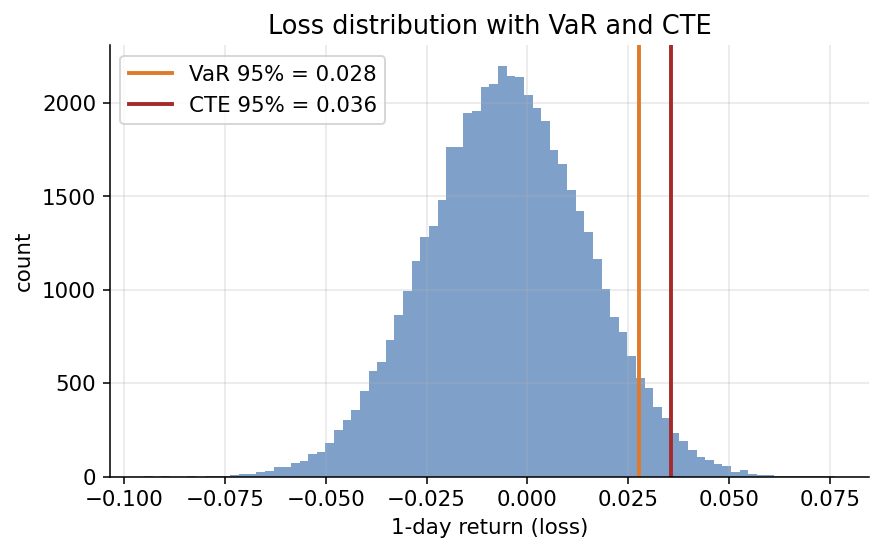
\includegraphics[keepaspectratio]{figures/ch09-var-cte.png}}
\emph{Loss distribution: VaR cutoff and CTE mean-loss beyond it.}

\subsection{15.2.1 Three computational routes to
VaR}\label{three-computational-routes-to-var}

Three methodologies dominate production risk systems: \emph{historical
simulation}, \emph{parametric (variance-covariance)}, and \emph{Monte
Carlo}. A well-run risk function uses at least two as cross-checks.

\textbf{Historical simulation.} Collect the last \(N\) daily P\&L
observations (the current portfolio re-priced under historical market
moves), sort them worst to best, and pick the \((1-\alpha)\)-quantile
directly. With \(N = 500\) and \(\alpha = 0.95\), the 95\% VaR is the
25th worst observation. The method is non-parametric: it makes no
distributional assumption, letting whatever fat tails, skew, and jumps
appeared historically carry through. Strengths: no model risk from
mis-specified distributions, trivial to explain. Weaknesses: only as
good as its lookback window, assigns equal weight to old and new
observations so regime shifts are absorbed with lag, and tail estimation
at \(\alpha = 0.99\) with \(N = 500\) rests on five data points.
Refinements include \emph{age-weighted} historical simulation (older
observations get less weight), \emph{volatility-scaled} historical
simulation (rescale each historical return by current-to-historical vol
ratio), and \emph{filtered historical simulation} (fit a GARCH model,
scale out historical vol, pick a quantile of residuals, scale back up by
current vol).

\textbf{Parametric / variance-covariance / delta-normal VaR.} Assume
portfolio returns are Gaussian with zero mean and variance
\(\sigma_P^2 = w^{\top} \Sigma w\), where \(w\) is the vector of dollar
exposures and \(\Sigma\) is the factor covariance matrix. Then

\[
\mathrm{VaR}_\alpha = z_{1-\alpha}\,\sigma_P = z_{1-\alpha}\,\sqrt{w^{\top} \Sigma w}, \tag{15.2}
\]

where \(z_{1-\alpha}\) is the Gaussian quantile (1.645 at 95\%, 2.326 at
99\%). Strengths: closed-form, fast even for very large portfolios,
decomposable cleanly by factor or asset class. Weaknesses: the Gaussian
assumption dramatically under-estimates fat-tail risk, and the linear
approximation to book P\&L fails for option-heavy books. Parametric VaR
is sometimes called ``delta-normal'' precisely because it couples a
linear delta approximation of position P\&L with a Normal distribution
of factor returns.

A partial fix for non-linearity is \emph{delta-gamma parametric VaR}:
approximate book P\&L by a quadratic function of risk factors,

\[
\Delta P \approx \delta^{\top} \Delta r + \tfrac{1}{2}\,\Delta r^{\top} \Gamma\,\Delta r, \tag{15.3}
\]

where \(\delta\) is the gradient of P\&L with respect to risk factors
and \(\Gamma\) is the Hessian. Under multivariate Normal \(\Delta r\)
the distribution of \(\Delta P\) is a quadratic form in Normals --- a
generalised chi-squared --- whose VaR can be obtained by Cornish-Fisher
expansion or numerical inversion of its characteristic function. We
develop this in full in §15.12; for now, note that delta-gamma
parametric VaR improves meaningfully on delta-normal for option-heavy
portfolios while retaining the Gaussian factor assumption.

\textbf{Monte Carlo VaR.} Specify a joint distribution for risk factor
returns (Gaussian, Student-\(t\), copula-based, stochastic-volatility,
full economic-scenario generator), draw simulated paths, reprice the
entire portfolio under each, and take the empirical quantile of the
simulated P\&L distribution. Strengths: flexibility to handle arbitrary
distributions, full non-linear pricing including path-dependent payoffs,
easy incorporation of complex instruments. Weaknesses: expensive (tens
of thousands of full-portfolio revaluations), model-risk-prone (the
joint distribution has to be specified and will be wrong in some way),
and slow to converge in the tail. Many large banks run Monte Carlo VaR
as the primary regulatory measure and historical simulation as a
cross-check.

A sample-size calculation is instructive. The standard error of a
quantile estimate based on \(M\) i.i.d. samples scales as
\(1/\sqrt{M \cdot f(q)^2 \cdot \alpha (1-\alpha)}\), where \(f(q)\) is
the density at the quantile. For a 99\% VaR with 10,000 Monte Carlo
paths under a Normal approximation, the standard error is 3-5\% of the
VaR itself. For 99.9\% VaR on the same 10,000 paths the standard error
blows up to 15-20\%, which is why extreme quantiles require massive
simulation budgets (often 100,000 paths or more) and motivate heavy use
of variance-reduction techniques such as importance sampling. A common
refinement is to oversample the tail, run disproportionately many paths
in stressful scenarios, re-weight them, and estimate the tail quantile
with much higher precision.

\pandocbounded{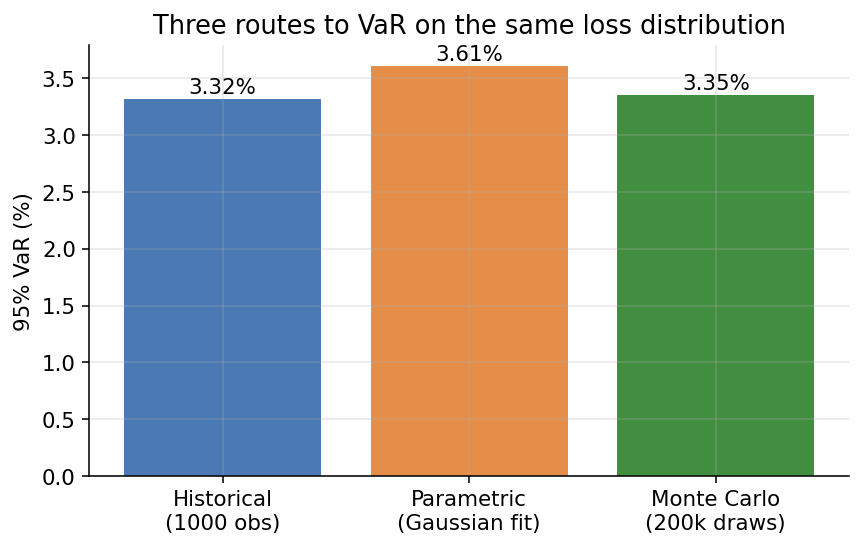
\includegraphics[keepaspectratio]{figures/ch09-var-three-routes.png}}
\emph{Historical, parametric (Gaussian), and Monte-Carlo estimates of
95\% VaR on the same skewed, jump-prone loss distribution. The Gaussian
fit systematically under-reports tail risk because it ignores the jump
component; historical and Monte-Carlo agree once the sample is large
enough to see the jump events. Running at least two methods in parallel
as cross-checks is standard production practice.}

\begin{figure}
\centering
\pandocbounded{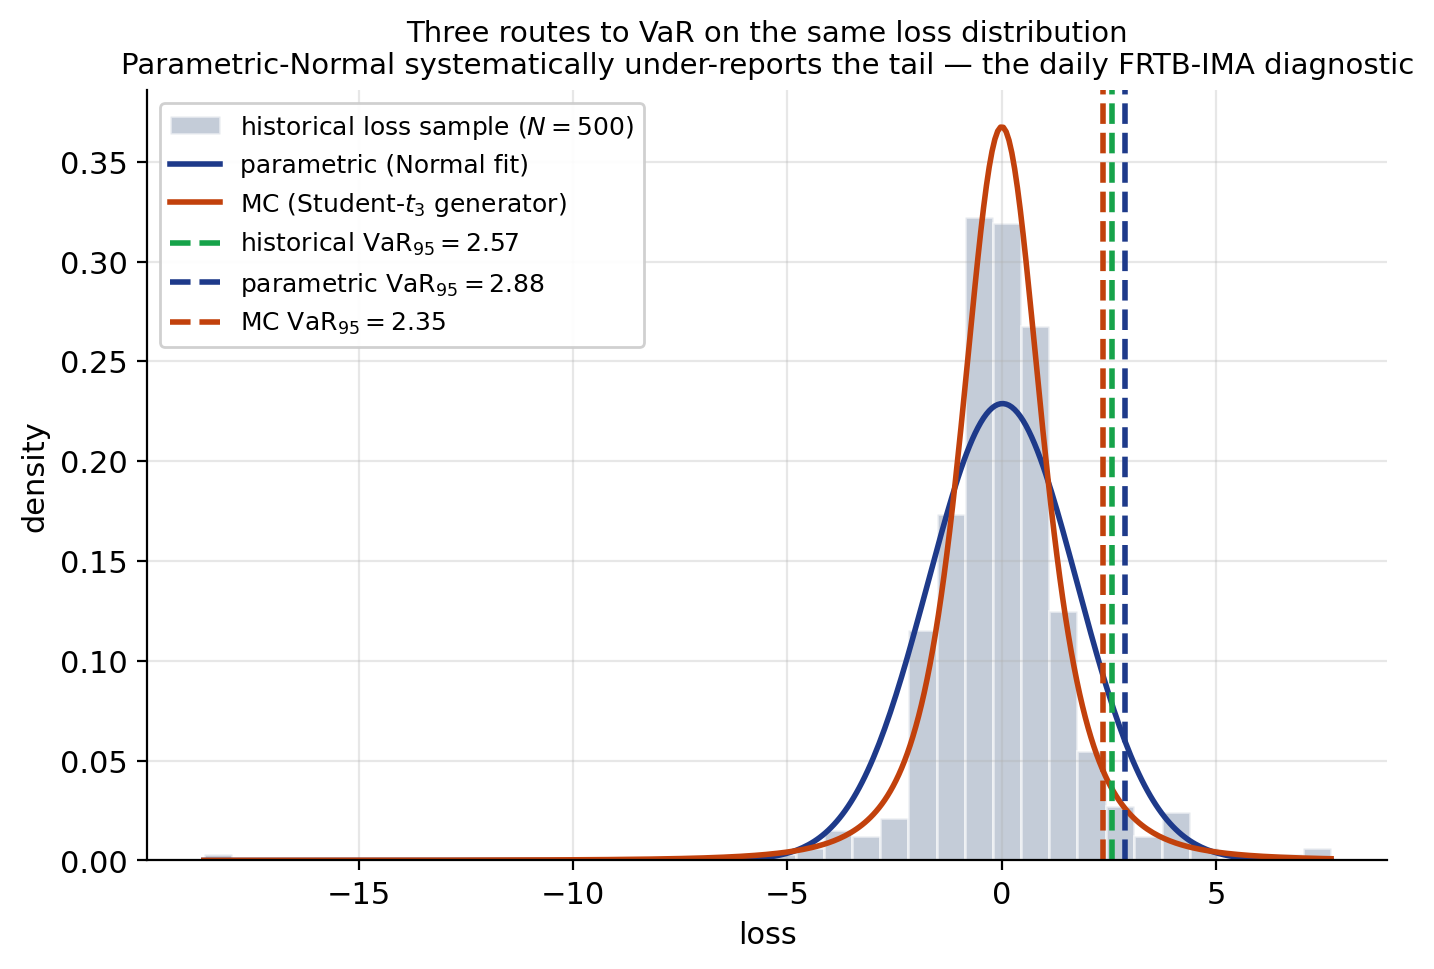
\includegraphics[keepaspectratio]{figures/ch15-three-routes-var.png}}
\caption{Historical, parametric, and MC VaR estimates on the same
Student-\(t_3\) loss sample: parametric-Normal systematically
under-reports the tail. The diagnostic any FRTB-IMA bank runs daily ---
and a corner of the analytical failure that left LTCM's daily VaR
overrun by roughly \(40\times\) on the worst August-1998 day (and an
order of magnitude more cumulatively)}
\end{figure}

\subsection{15.2.2 Cornish-Fisher
expansion}\label{cornish-fisher-expansion}

Between ``full Monte Carlo'' and ``pure Gaussian'' sits the
\emph{Cornish-Fisher expansion}, a semi-parametric trick that adjusts
the Gaussian quantile for skewness and excess kurtosis without a full
simulation. Express the true quantile of a non-Gaussian distribution as
a series in the standard Gaussian quantile:

\[
q_\alpha \approx z_\alpha + \tfrac{1}{6}(z_\alpha^2 - 1)\,s + \tfrac{1}{24}(z_\alpha^3 - 3 z_\alpha)\,\kappa - \tfrac{1}{36}(2 z_\alpha^3 - 5 z_\alpha)\,s^2, \tag{15.4}
\]

where \(z_\alpha\) is the Gaussian quantile, \(s\) is skewness, and
\(\kappa\) is excess kurtosis of the target distribution. Multiplying by
the portfolio standard deviation gives a skew-and-kurt-adjusted VaR. The
formula captures most of the correction needed for modestly non-Gaussian
P\&L distributions. For heavily non-Gaussian distributions --- deep fat
tails, severe skewness near crash events --- Cornish-Fisher breaks down
and Monte Carlo or historical simulation is required.

The practical appeal is enormous when combined with delta-gamma
parametric VaR. The quadratic form in (15.3) has skewness and kurtosis
computable in closed form from \(\delta\), \(\Gamma\), and \(\Sigma\).
Feeding those moments into (15.4) yields a VaR that incorporates both
non-linearity (via \(\Gamma\)) and distributional tail adjustment (via
skew/kurt), without a single Monte Carlo path. This
delta-gamma-Cornish-Fisher VaR was widely used in the 1990s and 2000s
and remains a useful benchmark.

\pandocbounded{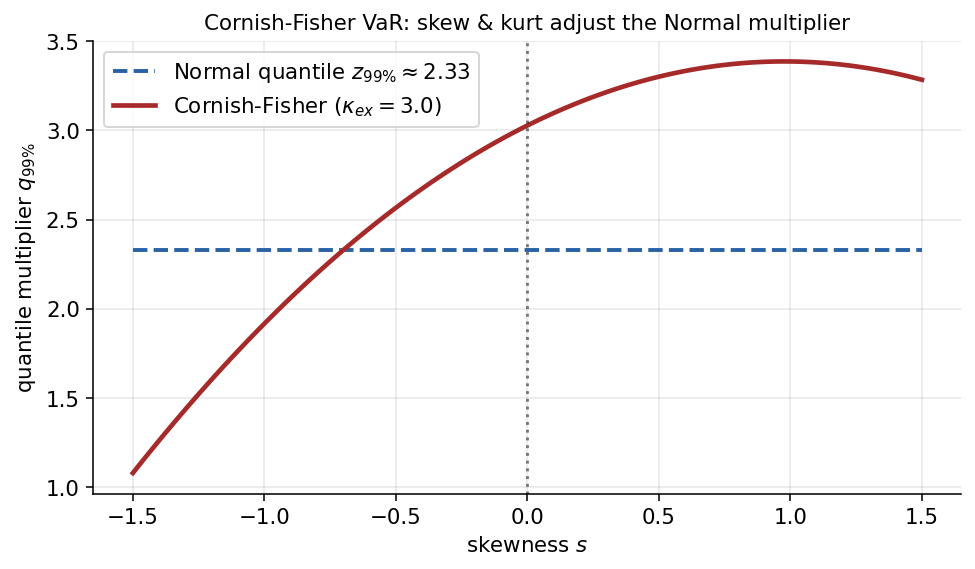
\includegraphics[keepaspectratio]{figures/ch09-cornish-fisher.png}}
\emph{The Cornish-Fisher quantile multiplier at \(99\%\) confidence as a
function of skewness (with excess kurtosis fixed at
\(\kappa_{\mathrm{ex}}=3\)). Negative skew (left tail heavy) raises the
multiplier above the Normal \(z_{99\%}\approx 2.33\); positive skew
pulls it down. A quadratic shape in \(s\) reflects the \(s^2\) term in
\((15.4)\).}

Two caveats. First, the expansion can produce non-monotonic quantile
functions for extreme parameter values (very fat tails, severe skew),
which makes no distributional sense. When this happens, the expansion is
signalling that the perturbation from Normal is too large to be captured
by a polynomial correction, and one must move to a full parametric or
non-parametric method. Second, skewness and excess kurtosis are
themselves very noisy to estimate from short time series --- sampling
standard errors are \(\sqrt{6/N}\) and \(\sqrt{24/N}\) respectively for
Gaussian data, meaning skew and kurt estimates from 250 days are nearly
useless. In practice, the moments are estimated from multi-year
histories or from a time-series model (GARCH, for example) that yields
more efficient estimates.

\subsection{15.2.3 Historical provenance and interpretive
tensions}\label{historical-provenance-and-interpretive-tensions}

VaR rose through the J.P. Morgan RiskMetrics framework in the early
1990s and was adopted by Basel as the regulatory standard for
market-risk capital; the appeal was operational (single number, easily
aggregated). The 2008 crisis shifted the regulatory consensus toward
expected shortfall. CVaR is theoretically superior but statistically
harder to backtest than VaR (exceedances are binomial; tail integrals
are not), which is why the modern compromise runs both --- VaR for
backtesting, CTE for capital.

\section{15.3 Conditional Tail Expectation and Expected
Shortfall}\label{conditional-tail-expectation-and-expected-shortfall}

\[
\mathrm{CTE}_\alpha(L) \;=\; \mathrm{ES}_\alpha(L) \;=\; \mathbb{E}\!\left[\,L \,\big|\, L \ge \mathrm{VaR}_\alpha(L)\,\right]. \tag{15.5}
\]

CTE (``conditional tail expectation'') and ES (``expected shortfall'')
refer to the same quantity. Where VaR only marks the threshold, CTE
integrates the tail \emph{beyond} it, so the two 5\%-tail scenarios from
§15.2 --- one fat, one thin --- earn different CTE scores. CTE is
coherent: monotone, positively homogeneous, translation-invariant, and
--- crucially --- sub-additive. The sub-additivity is what we need for
any risk axis on which diversification is guaranteed to help.

\begin{figure}
\centering
\pandocbounded{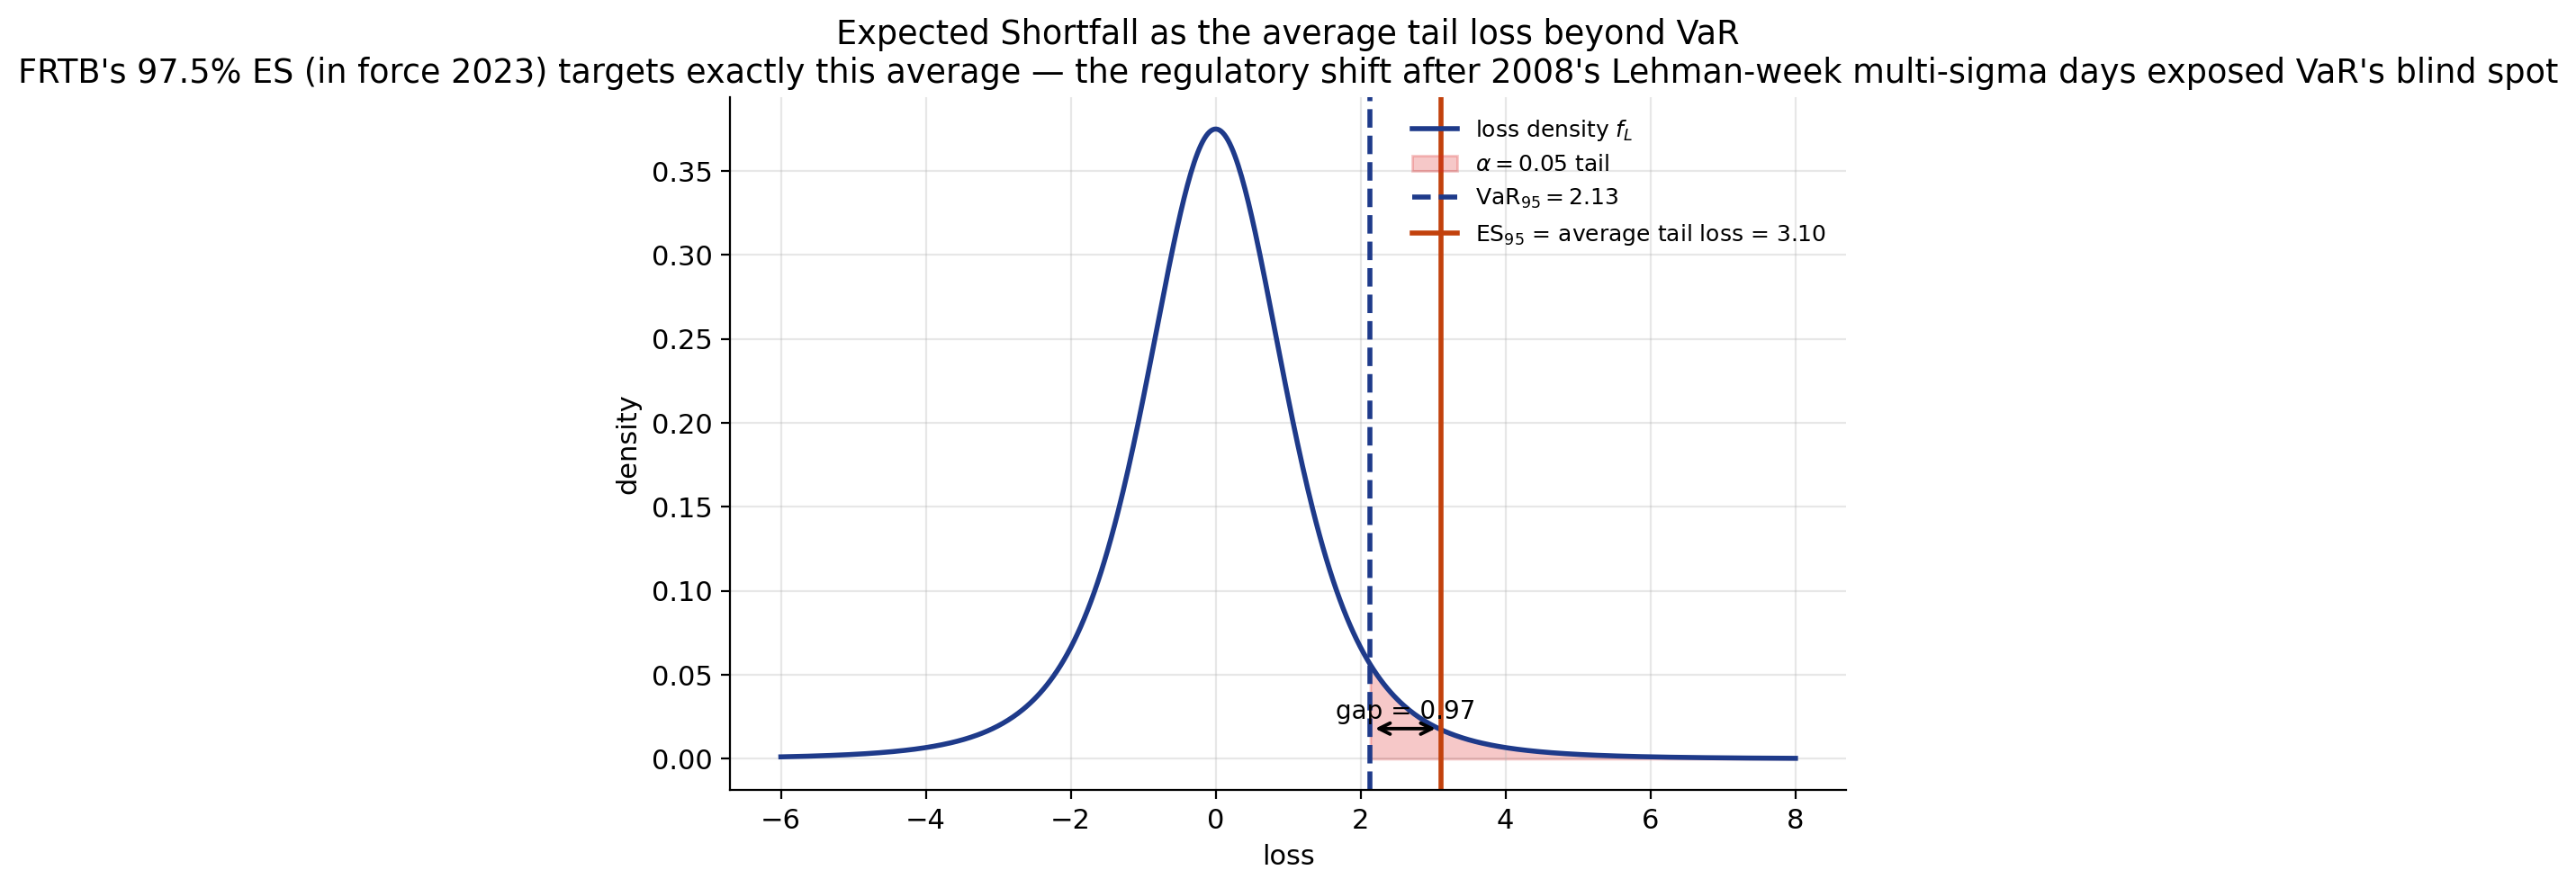
\includegraphics[keepaspectratio]{figures/ch15-es-tail-average.png}}
\caption{ES/CTE as the \emph{average} of losses beyond VaR\(_{95}\) on a
Student-\(t_4\) loss distribution: the gap ES \(-\) VaR is exactly the
average size of the loss conditional on entering the tail. FRTB's 97.5\%
ES (in force from 2023) targets this conditional average --- the
regulatory answer to VaR's well-known blind spot for tail magnitude}
\end{figure}

\textbf{Normal versus fat tail.} The thin-tailed Normal has VaR
\(\approx 1.64\) and CTE \(\approx 2.06\) at 95\% --- a gap of 0.4. For
a Student-\(t_3\) \emph{rescaled to unit variance} (i.e.~the base
\(t_3\) divided by \(\sqrt{\nu/(\nu-2)} = \sqrt{3}\) so both
distributions share zero mean and unit variance), the 95\% VaR is
\(\approx 2.35/\sqrt{3} \cdot \sqrt{3} = 2.35\) (retaining the
base-\(t_3\) quantile \(q_{0.05} \approx 2.353\) for this comparison
since the figure plots same-scale densities) and the CTE is
\(\approx 4.19\) --- a gap of 1.8, nearly five times larger. (On the
unscaled base-\(t_3\) convention, VaR \(\approx 2.35\) and CTE
\(\approx 2.34\); the qualitative ``CTE exceeds VaR by much more in the
fat-tailed case'' narrative holds under either convention, but the
specific 4.19 number uses the unit-variance rescaling so that the
comparison with the unit-variance Normal is apples-to-apples.) The
practical point: two books can share the same VaR yet have wildly
different CTE, which is precisely the pathology CTE was designed to
catch. In closed form for Student-\(t\) with \(\nu\) degrees of freedom,

\[
\mathrm{CTE}_\alpha^{t_\nu} = \frac{f_{t_\nu}(\mathrm{VaR}_\alpha^{t_\nu})\,\bigl(\nu + (\mathrm{VaR}_\alpha^{t_\nu})^2\bigr)}{(\nu - 1)\,\alpha}, \tag{15.6}
\]

where \(f_{t_\nu}\) is the Student-\(t\) density. The key observation is
the \((\nu - 1)\) denominator: as \(\nu \to 1\) (Cauchy), CTE diverges
while VaR remains finite. Even at \(\nu = 2\), CTE is finite but much
larger than VaR; at \(\nu = 3\) we get the 1.8-gap quoted above. As
\(\nu \to \infty\) the distribution approaches Normal and the gap
converges to the Normal value of 0.4. The tail-index \(\nu\)
interpolates smoothly between ``Normal-like'' and ``catastrophically
fat-tailed'', and CTE tracks the deterioration faithfully while VaR only
modestly responds.

\textbf{Why the switch happened.} Empirically estimated tail indices for
daily equity returns sit in the range 3-5 (4-7 for weekly);
emerging-market currencies and distressed credit can drop to 2, making
CTE much larger than VaR by a factor of several. Any risk framework that
relies on Normal-CTE benchmarks systematically under-reports tail risk
in these markets, and the under-reporting compounds during crisis
periods when the tail index temporarily shrinks further. Every blow-up
in the historical record of hedge funds and investment banks --- and a
depressing number of insurance companies --- can be traced, at least
partially, to a VaR that looked fine alongside a CTE that would have
screamed. The regulatory transition from 99\% VaR charges toward 97.5\%
CTE charges was a direct response.

The 97.5\% CTE calibration deserves explanation. For a Gaussian loss
distribution, \(\mathrm{CTE}_{97.5\%} \approx \mathrm{VaR}_{99\%}\), so
the switch was designed to leave the average capital charge roughly
unchanged but to make the charge responsive to tail shape. Fat-tailed
portfolios now face genuinely higher capital requirements than
thin-tailed portfolios with the same 99\% VaR. This is the regulatory
incentive-alignment the Basel Committee wanted: portfolios whose tails
actually matter are capitalised accordingly.

\textbf{Estimation is harder.} CTE estimation has a statistical subtlety
that VaR estimation does not. VaR is a quantile, determined by the local
behaviour of the CDF around a single point; estimation depends on the
density at that point. CTE is an integral over the tail, so estimation
depends on the density \emph{everywhere} in the tail, and density
estimates at extreme quantiles have high variance. A 99\% CTE from 250
daily returns is the mean of the 2.5 worst returns --- so it depends
heavily on the single \emph{worst} observation in the sample. If the
sample contains a mild outlier like -4\% the estimate comes in around
-3.5\%; if it contains a catastrophic -12\% like September 2008, the
estimate jumps to -7\% or worse. Two samples drawn from the same
underlying distribution can give CTE estimates that differ by a factor
of two even when their VaR estimates agree within basis points.

This sensitivity is a blessing and a curse. Blessing: CTE correctly
reflects genuine tail events when they occur --- the measure is
\emph{doing its job} by responding to extreme observations. Curse: CTE
estimates have wide confidence intervals, which makes it hard to tell
whether a day-over-day change reflects genuine risk change or sampling
noise. The pragmatic response is to model the tail parametrically using
a Generalised Pareto (GPD) fit to excesses over a threshold --- the
\emph{peaks-over-threshold} extreme-value technique developed in §15.4.
A GPD fit extrapolates the tail smoothly beyond observed data, giving
much more stable CTE at the cost of a modest parametric assumption.

\textbf{Elicitability and model comparison.} A risk measure is
\emph{elicitable} if it can be expressed as the minimiser of an expected
scoring function. VaR is elicitable (via quantile loss); CTE is not
elicitable in general. This matters for model comparison: to compare two
VaR forecasts we can use average quantile loss, and a lower score is
unambiguously better. For CTE no such scoring function exists, and
comparing two CTE models rigorously requires more elaborate tests ---
the Fissler-Ziegel joint elicitability of VaR and CTE, for instance.
Regulators continue to debate whether elicitability is essential; the
pragmatic view is that it is not, but its absence complicates the
model-validation toolkit.

\textbf{CTE as a portfolio-construction axis.} The VaR-minimising
portfolio on an efficient frontier is not generally the CTE-minimising
portfolio on the same frontier. Empirical studies have found that
mean-CTE-optimised portfolios can have 20-40\% lower crash losses than
mean-VaR-optimised portfolios even when their mean-variance
characteristics are similar. This is a second reason for the regulatory
shift toward CTE beyond measurement fidelity: CTE actively produces
better portfolios when used as an optimisation objective.

\pandocbounded{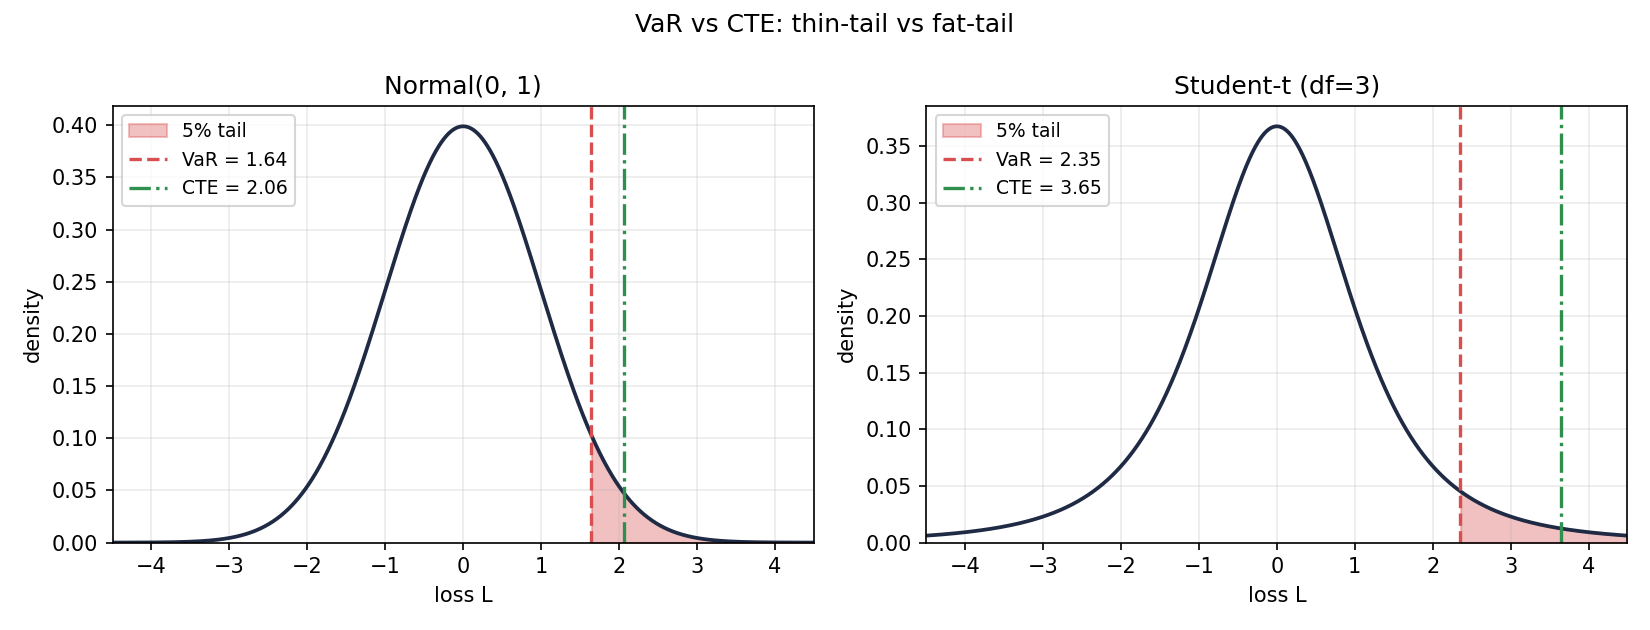
\includegraphics[keepaspectratio]{figures/ch09-var-cte-compare.png}}
\emph{VaR and CTE compared across Normal (thin tail) and Student-\(t_3\)
(fat tail) --- same quantile can hide very different tail masses.}

\begin{figure}
\centering
\pandocbounded{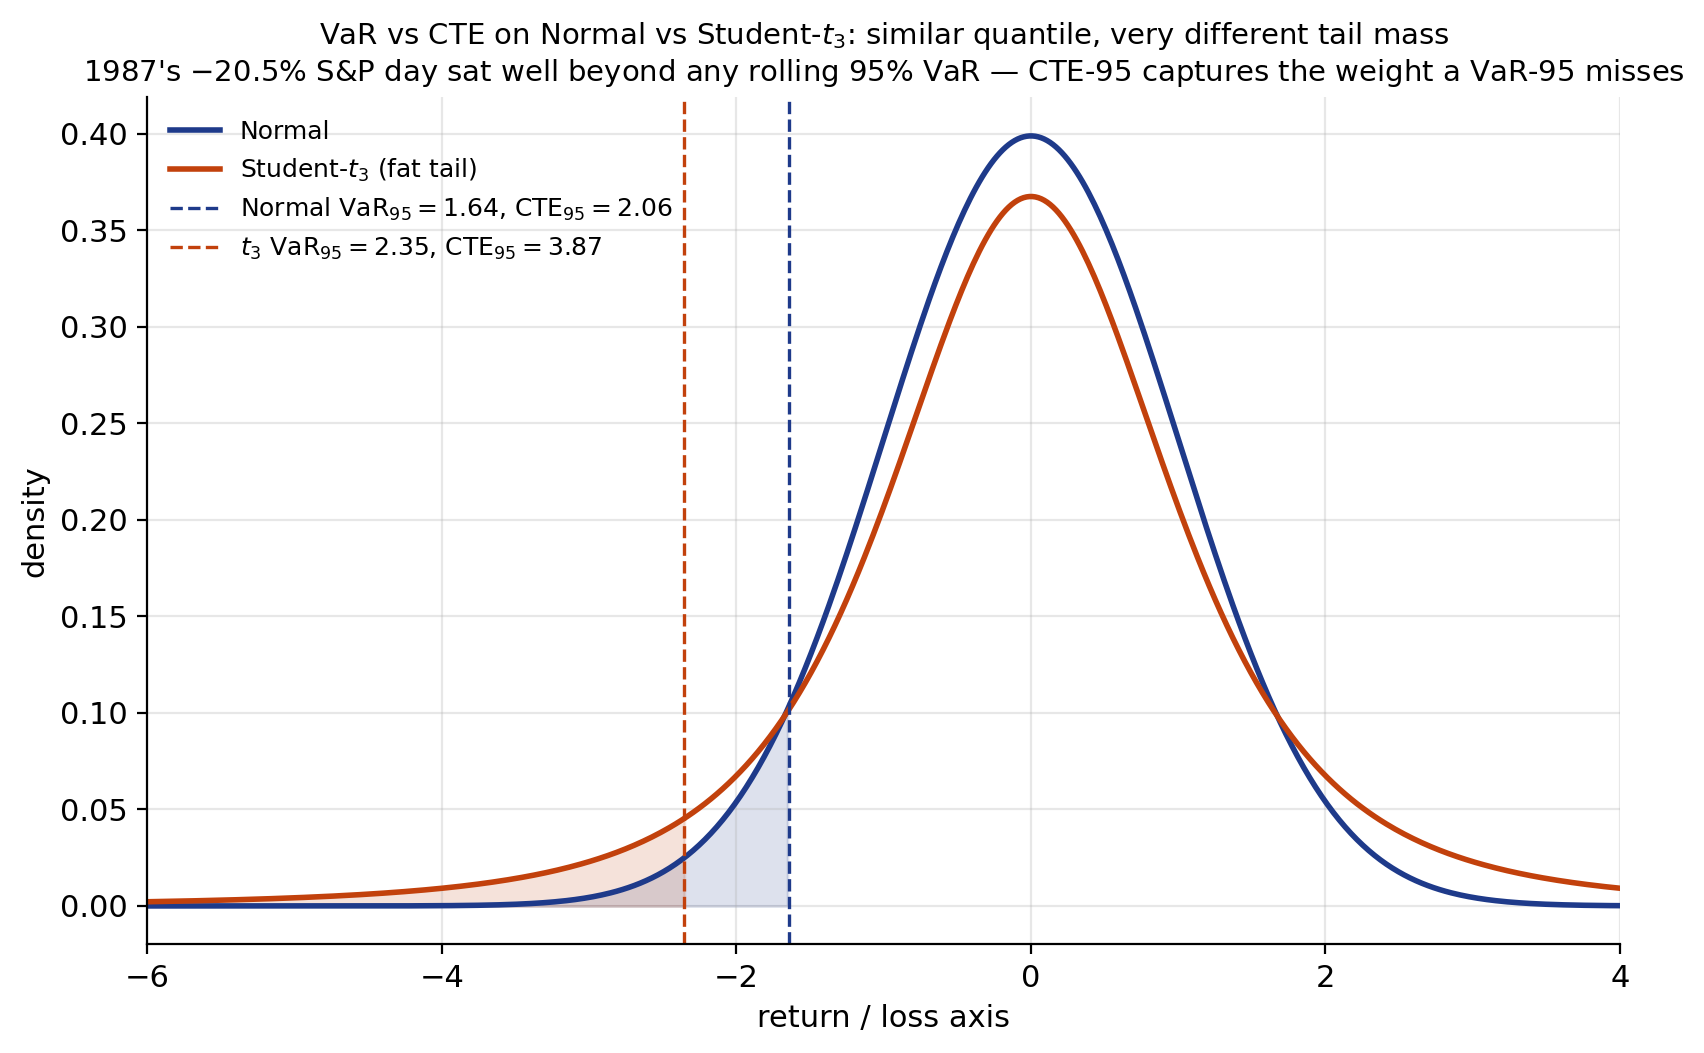
\includegraphics[keepaspectratio]{figures/ch15-var-cte-fat-tail.png}}
\caption{Densities of Normal vs Student-\(t_3\) with VaR\(_{95}\)
cutoffs marked and 5\% tails shaded: the CTE gap is far larger for the
fat tail. The 1987 \(-20.5\%\) S\&P 500 day (the DJIA fell \(-22.6\%\))
sat well beyond any rolling 95\% VaR --- exactly the kind of tail mass
CTE is built to capture}
\end{figure}

\section{15.4 Thin vs Fat Tails: Student-t and Extreme Value
Theory}\label{thin-vs-fat-tails-student-t-and-extreme-value-theory}

\pandocbounded{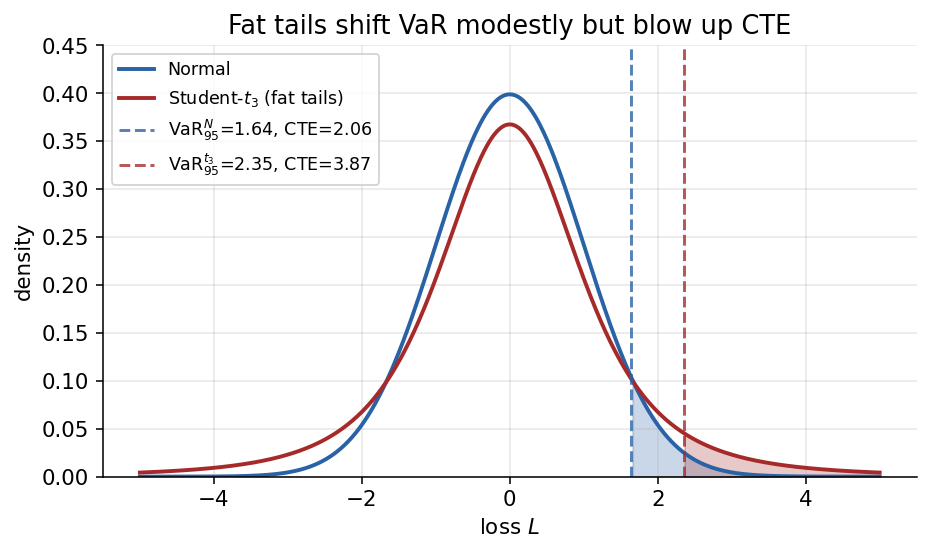
\includegraphics[keepaspectratio]{figures/ch09-normal-vs-t3.png}}
\emph{Same scale, very different tails. The 95\% VaR cutoffs differ
modestly (Normal \(1.64\) vs Student-\(t_3\) \(2.35\)), but the CTE
values diverge dramatically (\(2.06\) vs \(4.19\)). VaR is a threshold;
CTE integrates the tail beyond it, and the ratio CTE/VaR is diagnostic
of tail-fatness.}

Under a Normal assumption, three-sigma losses occur with probability
\(0.13\%\)/day; under Student-\(t_3\) at matching scale, the same
threshold has probability \(\approx 2.5\%\), twenty times more often.
Equity indices, EM currencies, and credit spreads sit closer to the
\(t\) picture than to Normal --- especially during crises. The 5σ/7σ/10σ
multi-day runs reported by major desks in 2008 and March 2020 were not
``once-per-age-of-the-universe'' Normal events; they were ordinary
Student-\(t\) tail observations whose Normal label was a mislabel.

\subsection{15.4.1 Defensive adjustments}\label{defensive-adjustments}

Three practical adjustments improve on Normal VaR without requiring a
full rewrite of the risk infrastructure.

\textbf{Parametric fat-tail fit.} Fit losses with a Student-\(t\),
skew-\(t\), or Generalised Hyperbolic distribution, estimate the degrees
of freedom from the data, and recompute VaR and CTE under the fitted
distribution. Even a rough fit with \(\nu = 5\) or \(\nu = 6\) captures
most of the relevant fat-tail behaviour. Maximum-likelihood or
method-of-moments estimation on a 3-5 year daily history gives
reasonably stable parameters; shorter windows give noisy \(\nu\)
estimates that can swing between 3 and 10 over successive weeks.

\textbf{Empirical historical simulation.} Compute VaR and CTE directly
from the realised P\&L history. This by construction inherits whatever
tail the market produced during the lookback window. It is the simplest
way to avoid mis-specifying the tail because it does not specify the
tail at all --- but it equally cannot extrapolate beyond the historical
sample.

\textbf{Explicit stress scenarios.} Layer historical stress scenarios
(Black Monday 1987, Lehman 2008, COVID 2020) and hypothetical scenarios
chosen by the risk committee on top of the parametric tail as a form of
risk insurance. The full stress-testing methodology is developed in
§15.8.

\subsection{15.4.2 Extreme Value Theory}\label{extreme-value-theory}

A more sophisticated methodology is \emph{Extreme Value Theory (EVT)},
which rests on a fundamental asymptotic result: the Pickands-Balkema-de
Haan theorem. For a wide class of loss distributions, the conditional
distribution of exceedances over a high threshold \(u\) converges to the
Generalised Pareto Distribution (GPD) as \(u \to \infty\):

\[
F_u(y) \;=\; \mathbb{P}(L - u \le y\,|\,L > u) \;\approx\; 1 - \left(1 + \xi \frac{y}{\beta}\right)^{-1/\xi}, \quad y > 0, \tag{15.7}
\]

with shape parameter \(\xi\) and scale parameter \(\beta > 0\). The sign
of \(\xi\) classifies the tail: \(\xi > 0\) is Fréchet (power-law tails,
infinite moments above order \(1/\xi\)), \(\xi = 0\) is Gumbel
(exponential tails), \(\xi < 0\) is Weibull (bounded tails). Equity
indices typically give \(\xi\) in the range 0.2-0.4; sovereign-rate
moves give \(\xi\) near 0; commodity returns can give \(\xi > 0.5\)
during shortage regimes.

The \emph{peaks-over-threshold} (POT) procedure is: pick a threshold
\(u\) (often the 90th or 95th percentile of observed losses), collect
the exceedances \(\{L_i - u : L_i > u\}\), fit \((\xi, \beta)\) by
maximum likelihood, and extrapolate the fitted GPD to obtain tail
quantiles and conditional tail expectations at confidence levels far
beyond the empirical data. A related technique uses the \emph{Hill
estimator} to estimate \(\xi\) directly from the ratio of the largest
order statistics of the sample --- simpler to implement but less
efficient than MLE.

The advantage of EVT over pure historical simulation is smooth
extrapolation beyond the observed data, giving stable estimates even at
extreme confidence levels (99.9\%, 99.99\%) where raw historical data
contains only a handful of observations. The disadvantage is that EVT
requires a threshold choice (too low and the asymptotic theorem fails to
apply well; too high and the fit loses data) and is sensitive to the
estimated shape \(\xi\), which has its own uncertainty.

\subsection{15.4.3 GARCH and conditional
dynamics}\label{garch-and-conditional-dynamics}

A complementary framework is the \emph{GARCH} family of volatility
models. GARCH (and its variants EGARCH, GJR-GARCH, TGARCH) captures the
\emph{clustering} of volatility --- high-vol periods persist --- and the
asymmetry of vol response to signed shocks (the leverage effect, where
bad news raises vol more than equally-sized good news). A GARCH-filtered
historical simulation takes GARCH residuals (returns divided by
conditional volatility), samples from the residual empirical
distribution, rescales by the forecast volatility, and computes VaR.
This hybrid combines the parametric strength of GARCH in modelling
volatility dynamics with the non-parametric strength of empirical
residuals in capturing fat tails, and is widely considered a
gold-standard methodology for equity and FX risk.

The chapter's emphasis on VaR and CTE as \emph{different} summaries of
the same loss distribution is really an emphasis on the limits of any
single-number summary. The loss distribution is the primary object; VaR
and CTE are two projections of it onto the real line. When the
distribution is Normal, VaR and CTE at any level are almost
interchangeable. When it is fat-tailed, they diverge dramatically, and
the divergence itself is diagnostic: a VaR-to-CTE ratio well above the
Gaussian benchmark is a red flag that the tail is mis-modelled.

\section{15.5 Basel Context and Regulatory
Capital}\label{basel-context-and-regulatory-capital}

The Basel framework determines which risk measures have operational
primacy at large banks. The headline evolution is the move from 99\% VaR
(Basel Market Risk Amendment 1996) to 97.5\% expected shortfall (FRTB
2016/2019, in force from 2023). The calibration was designed so that
under a Gaussian loss distribution the two produce roughly the same
charge --- \(\mathrm{CTE}_{97.5\%}\approx \mathrm{VaR}_{99\%}\) ---
while making the charge \emph{responsive to tail shape}: fat-tailed
books now consume more capital than thin-tailed books at the same 99\%
VaR.

{\def\LTcaptype{none} % do not increment counter
\begin{longtable}[]{@{}
  >{\raggedright\arraybackslash}p{(\linewidth - 6\tabcolsep) * \real{0.2500}}
  >{\raggedright\arraybackslash}p{(\linewidth - 6\tabcolsep) * \real{0.2500}}
  >{\raggedright\arraybackslash}p{(\linewidth - 6\tabcolsep) * \real{0.2500}}
  >{\raggedright\arraybackslash}p{(\linewidth - 6\tabcolsep) * \real{0.2500}}@{}}
\toprule\noalign{}
\begin{minipage}[b]{\linewidth}\raggedright
Accord
\end{minipage} & \begin{minipage}[b]{\linewidth}\raggedright
Year
\end{minipage} & \begin{minipage}[b]{\linewidth}\raggedright
Market-risk measure
\end{minipage} & \begin{minipage}[b]{\linewidth}\raggedright
Notable additions
\end{minipage} \\
\midrule\noalign{}
\endhead
\bottomrule\noalign{}
\endlastfoot
Basel I & 1988 & (credit only) & RWA, 8\% capital ratio \\
Market Risk Amendment & 1996 & 10-day 99\% VaR (IMA) & Traffic-light
backtesting; \(k\ge 3\) multiplier \\
Basel II / 2.5 & 2004/2009 & VaR + stressed VaR & IRB; IRC for credit
migration \\
Basel III & 2010/13 & VaR (unchanged) & Leverage ratio, LCR/NSFR \\
FRTB & 2016/19 & 97.5\% ES & Liquidity horizons; NMRF; PLA test \\
\end{longtable}
}

In parallel with IMA, banks can elect the Standardised Approach (SA):
simpler, typically higher capital, and the fallback if IMA is revoked
for failed backtesting.

\section{15.6 The Coherent Risk
Framework}\label{the-coherent-risk-framework}

A risk measure \(\rho\) acting on a space of random losses is
\emph{coherent} in the Artzner-Delbaen-Eber-Heath sense if it satisfies
four axioms. We state them in the loss convention (large positive =
painful), and unpack each in turn.

\textbf{Monotonicity (M).} \(L_1 \le L_2\) almost surely
\(\Rightarrow \rho(L_1) \le \rho(L_2)\). A strictly smaller-loss random
variable must have a smaller risk measure. This is the bare-minimum
sanity requirement and both VaR and CTE satisfy it. (In the
\emph{profit} convention used by Artzner et al.'s original paper and
some other sources, monotonicity reads
\(X_1 \le X_2 \Rightarrow \rho(X_1) \ge \rho(X_2)\) --- bigger wealth
means smaller risk --- so readers cross-referencing should flip the
inequality alongside the sign convention.)

\textbf{Translation invariance (TI).} \(\rho(L + c) = \rho(L) + c\) for
any constant \(c\). Adding a deterministic dollar of loss adds a dollar
of risk. Note the sign: adding a deterministic dollar of \emph{profit}
(so \(c < 0\)) reduces the risk by a dollar --- this is the ``cash can
be netted against risk'' statement underlying capital-charge accounting.

\textbf{Positive homogeneity (PH).}
\(\rho(\lambda L) = \lambda \rho(L)\) for \(\lambda \ge 0\). Doubling
every position doubles the risk. Both VaR and CTE comply. One can argue
the axiom is too clean --- very large positions face liquidity haircuts
and \(\rho(10 L)\) should probably exceed \(10 \rho(L)\) --- but the
classical framework ignores such frictions.

\textbf{Sub-additivity (S).}
\(\rho(L_1 + L_2) \le \rho(L_1) + \rho(L_2)\). This formalises
``diversification never hurts.'' It is what VaR fails and CTE (under
mild regularity conditions) obeys.

\subsection{15.6.1 The sub-additivity failure of
VaR}\label{the-sub-additivity-failure-of-var}

To see the VaR failure concretely, take two independent loans, each of
which defaults with probability 4\% producing a loss of 100, and
otherwise pays zero. Individually, the 95\% VaR of each is 0 --- a 4\%
tail event does not breach the 5\% confidence line. But the sum can
default twice, once, or not at all. The probability of at least one
default is roughly 8\%, of two defaults about 0.16\%, so the 95\% VaR of
the merged book is around 100, not 0. Merging two risks whose individual
VaRs are zero gave a combined VaR of 100.

\pandocbounded{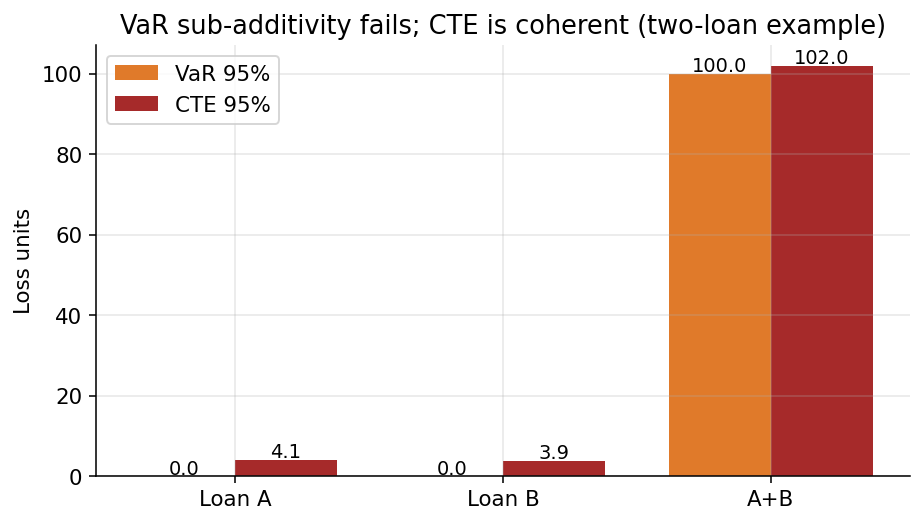
\includegraphics[keepaspectratio]{figures/ch09-subadditivity-failure.png}}
\emph{Monte-Carlo verification of the two-loan thought experiment: each
loan has VaR\(_{95} = 0\) in isolation, but their sum has
VaR\(_{95} \approx 100\). CTE is coherent --- the merged CTE is bounded
by the sum of individual CTEs --- and so can serve as a risk-budgeting
axis where VaR cannot.}

\begin{figure}
\centering
\pandocbounded{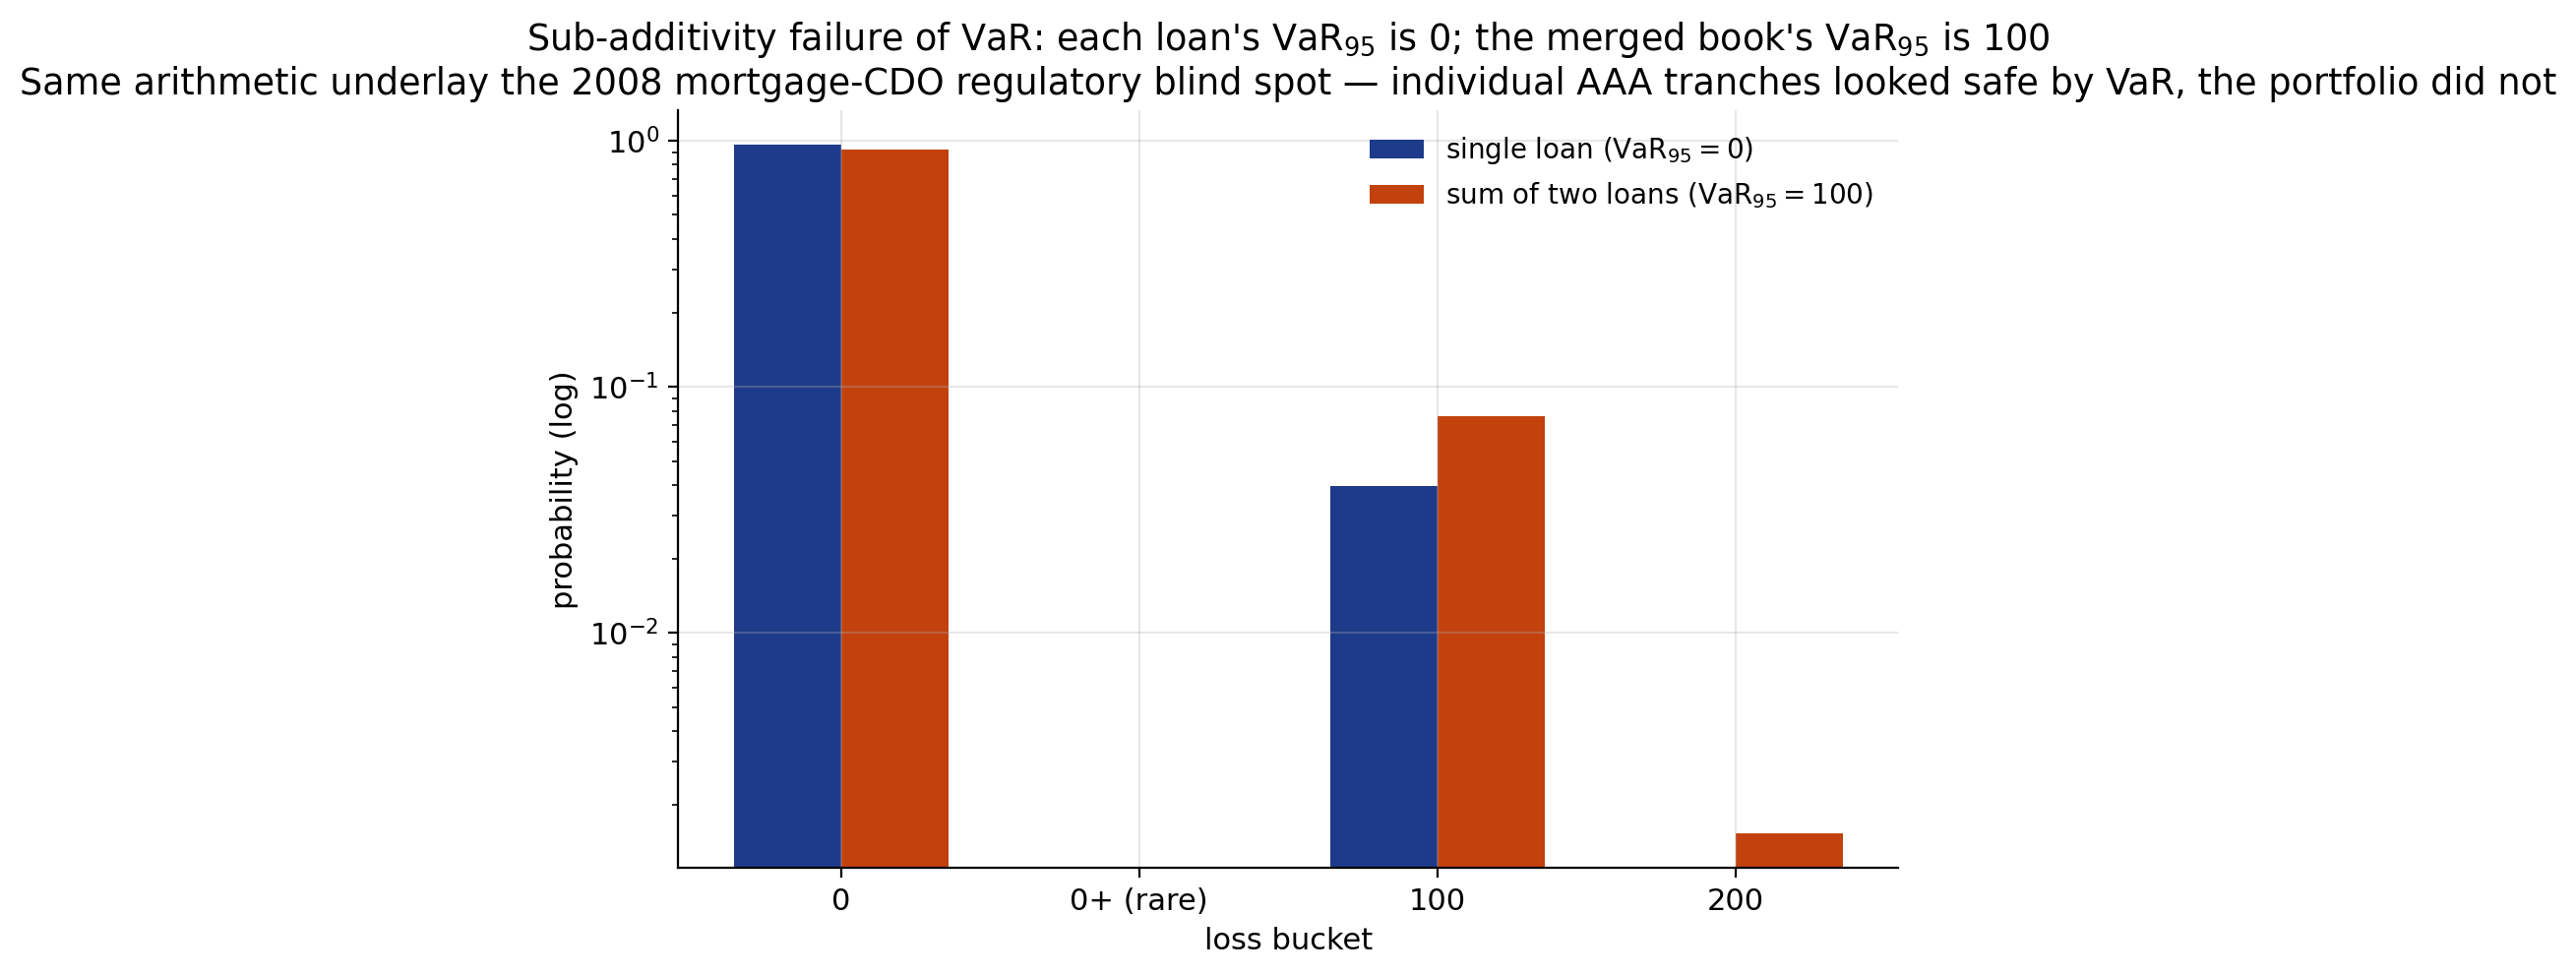
\includegraphics[keepaspectratio]{figures/ch15-subadditivity-violation.png}}
\caption{Loss-bucket probability comparison: each single loan's
\(95\%\)-VaR is 0, the merged sum's is 100. Same arithmetic underlay the
2008 senior-CDO regulatory blind spot --- individual AAA tranches looked
safe by VaR, the portfolio did not}
\end{figure}

The pathology is generic to any loss distribution with mass concentrated
just inside the VaR threshold. It afflicts credit books particularly
badly because individual defaults are exactly such
low-probability-high-impact events: an investment-grade bond has a
1-year default probability under 1\%, well below the 5\% VaR threshold,
so its individual VaR is zero. A portfolio of thousands of such bonds
has a default frequency of tens per year and generates substantial
portfolio VaR. If we used VaR to set capital on individual loans we
would allocate zero, yet the portfolio clearly needs substantial
capital. The CTE-based alternative assigns positive CTE even to
individual low-probability defaults --- because the tail expectation
averages over the default scenario --- and produces a portfolio CTE that
equals the sum of individual CTEs minus diversification benefits. A much
more coherent story.

A corollary of sub-additivity failure: VaR cannot serve as a direct
basis for risk-budget allocation. If desk A has VaR \$1M and desk B has
VaR \$1M, the firm's VaR is \emph{not generally} \$2M or anything
derivable from the individual VaRs. It could be \$0.5M (perfectly
negatively correlated), \$1.4M (independent), \$2M (perfectly
correlated), or \$2.2M (the pathological failure). The bank has no way
of allocating \$2M of firm-level VaR to desk-level budgets using just
the desk VaRs. CTE, being sub-additive, allows clean Euler-style
decomposition, and this is part of the technical appeal of using CTE as
the desk-level budgeting tool even when VaR is reported to regulators.

\subsection{15.6.2 The dual representation and spectral
measures}\label{the-dual-representation-and-spectral-measures}

The foundational theorem of coherent risk is a \emph{dual
representation}: every coherent \(\rho\) can be written as a worst-case
expectation over a set \(\mathcal{Q}\) of probability measures,

\[
\rho(L) \;=\; \sup_{\mathbb{Q} \in \mathcal{Q}} \mathbb{E}^{\mathbb{Q}}[L]. \tag{15.8}
\]

This unifies many apparently different risk measures under a single
umbrella: every coherent risk measure is a worst-case expectation over
some class of scenarios. CTE at level \(\alpha\) corresponds to taking
\(\mathcal{Q}\) to be the set of probability measures that are
absolutely continuous with respect to the base measure with a
Radon-Nikodym derivative bounded by \(1/\alpha\). VaR does not admit
such a representation because it is not coherent.

A richer parametric family is the class of \emph{spectral risk
measures}, each of which can be written as a weighted average of
quantiles:

\[
\rho_\phi(L) \;=\; \int_0^1 \phi(u)\,F_L^{-1}(u)\,du, \tag{15.9}
\]

where \(\phi : [0,1] \to [0, \infty)\) is a non-decreasing weighting
function with \(\int \phi = 1\). VaR at level \(\alpha\) corresponds to
\(\phi\) being a Dirac delta at \(u = 1 - \alpha\) --- all weight on a
single quantile --- and is not coherent because the spike violates
monotonicity of \(\phi\). CTE at level \(\alpha\) corresponds to uniform
weighting \(\phi(u) = \mathbf{1}_{u \ge 1-\alpha}/\alpha\) over the tail
--- coherent because \(\phi\) is non-decreasing. One can imagine
\(\phi\) functions that assign even more aggressive weight to the
extreme tail, producing risk measures that interpolate between ``care
only about one quantile'' (VaR) and ``care linearly about the whole tail
mean'' (CTE) and beyond into ``care hyperbolically about the extreme
tail.'' The desk-level upshot: CTE is a sensible default but not a
unique answer; a catastrophe-reinsurance book might prefer a more
tail-weighted spectral measure still.

\textbf{Coherence is a minimum bar, not the last word.} Coherence
formalises ``not broken''; measures that fail it can still be
operationally useful (VaR as a communicable summary) but must be
supplemented by a coherent companion (CTE for the tail shape; stress
scenarios for catastrophes) before the suite is diagnostically adequate.

\subsection{15.6.3 Case study --- three failures of VaR
(preview)}\label{case-study-three-failures-of-var-preview}

The coherent-risk framework just developed is the analytical residue of
three crises that the dominant risk measure of the day did not survive:
LTCM (\(1998\)), Archegos (\(2021\)), and the \(2008\) GFC. Each is
treated in full in the \textbf{Case studies --- three failures of VaR}
section near the end of this chapter, with the chapter-wide machinery
serving as the analytical lens. As a preview: LTCM's headline \(\$45\)M
VaR underestimated the realised six-week loss of \(\$4.6\)B by
\(\sim 100\times\) because the historical sample contained no
crisis-correlation regime; Archegos's per-PB VaRs each looked manageable
but the cross-PB consolidated exposure (which no single PB could see)
totalled \(\$80\)B and produced \(\$10\)B+ of bank losses; and
pre-\(2008\) Basel-II VaR on senior CDO tranches missed
correlated-default tails because mortgage-asset correlation was
calibrated at \(0.30\) on a benign housing regime and went to \(0.95\)
in \(2007\)--\(2008\). These three episodes motivate the rest of the
chapter: backtesting (§15.7) to detect regime breaks, stress testing
(§15.8) to insert events the historical window omits, risk decomposition
(§15.9) to flag concentration, and CTE/ES (§15.3) as the measure that
actually reports the size of the tail.

\section{15.7 Backtesting: Kupiec and
Christoffersen}\label{backtesting-kupiec-and-christoffersen}

Once a VaR model is in production, it must be validated against realised
P\&L. The framework for this validation is \emph{backtesting}: compare
the daily sequence of reported VaRs against the daily sequence of
realised P\&Ls, count exceedances (days on which the realised loss
exceeded the VaR), and apply statistical tests to decide whether the
exceedance pattern is consistent with the model.

\subsection{15.7.1 The exceedance indicator and its expected
behaviour}\label{the-exceedance-indicator-and-its-expected-behaviour}

Define the exceedance indicator

\[
I_t \;=\; \mathbf{1}\{L_t > \mathrm{VaR}_{\alpha,t}\}. \tag{15.12}
\]

If the VaR model is correctly calibrated at confidence level
\((1 - \alpha)\), then each \(I_t\) is a Bernoulli\((\alpha)\) random
variable and the sequence \(\{I_t\}\) is i.i.d. (independent because
past exceedances should carry no information about today, identically
distributed because the tail probability is by construction \(\alpha\)
every day). Both the ``correct frequency'' claim and the ``correct
independence'' claim are empirically testable.

\subsection{15.7.2 Kupiec's proportion-of-failures
test}\label{kupiecs-proportion-of-failures-test}

The simplest test --- targeting frequency --- is Kupiec's POF test. Over
\(n\) days, let \(x = \sum_t I_t\) be the number of exceedances. Under
the null that the model is correct, \(X \sim\) Binomial\((n, \alpha)\)
with mean \(n\alpha\) and variance \(n\alpha(1 - \alpha)\). The
likelihood-ratio statistic is

\[
\mathrm{LR}_{\mathrm{POF}} \;=\; -2 \log\!\left[\frac{\alpha^x (1 - \alpha)^{n - x}}{\hat{p}^x (1 - \hat{p})^{n - x}}\right], \qquad \hat{p} = \frac{x}{n}, \tag{15.13}
\]

asymptotically \(\chi^2_1\) under the null. Reject at 5\% significance
if \(\mathrm{LR}_{\mathrm{POF}} > 3.84\). For a 99\% VaR with
\(n = 250\) days, expected exceedances are \(n\alpha = 2.5\); the test
rejects above about 7 exceedances or at 0 (which is paradoxically
\emph{too few}, suggesting the model is too conservative and
over-capitalising the book).

This is the essence of the Basel ``traffic light'' regime. More than 4
exceedances in a 250-day window puts the model in the yellow zone
(capital multiplier \(k\) rises from 3.00 by 0.4-0.85 depending on
count); more than 9 exceedances puts it in the red zone (multiplier
capped at 4.00, pending a full model revision). Capital is directly tied
to backtest performance, giving banks a strong financial incentive to
build models that actually work.

\pandocbounded{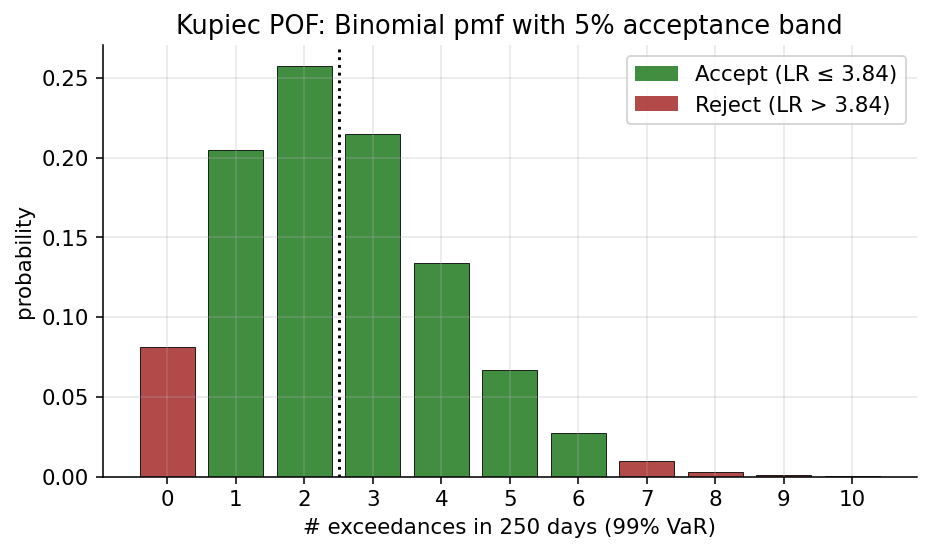
\includegraphics[keepaspectratio]{figures/ch09-kupiec-band.png}}
\emph{Binomial pmf of exceedance counts under the null
\(X\sim\mathrm{Binomial}(250,\,0.01)\), coloured green where the Kupiec
likelihood-ratio is below the \(5\%\) critical value \(3.84\) and red
where it rejects. Green bars span roughly \(0\)--\(6\) exceedances;
beyond that the model is rejected as under-capitalised. Zero exceedances
is technically also rejected as over-conservative.}

\begin{figure}
\centering
\pandocbounded{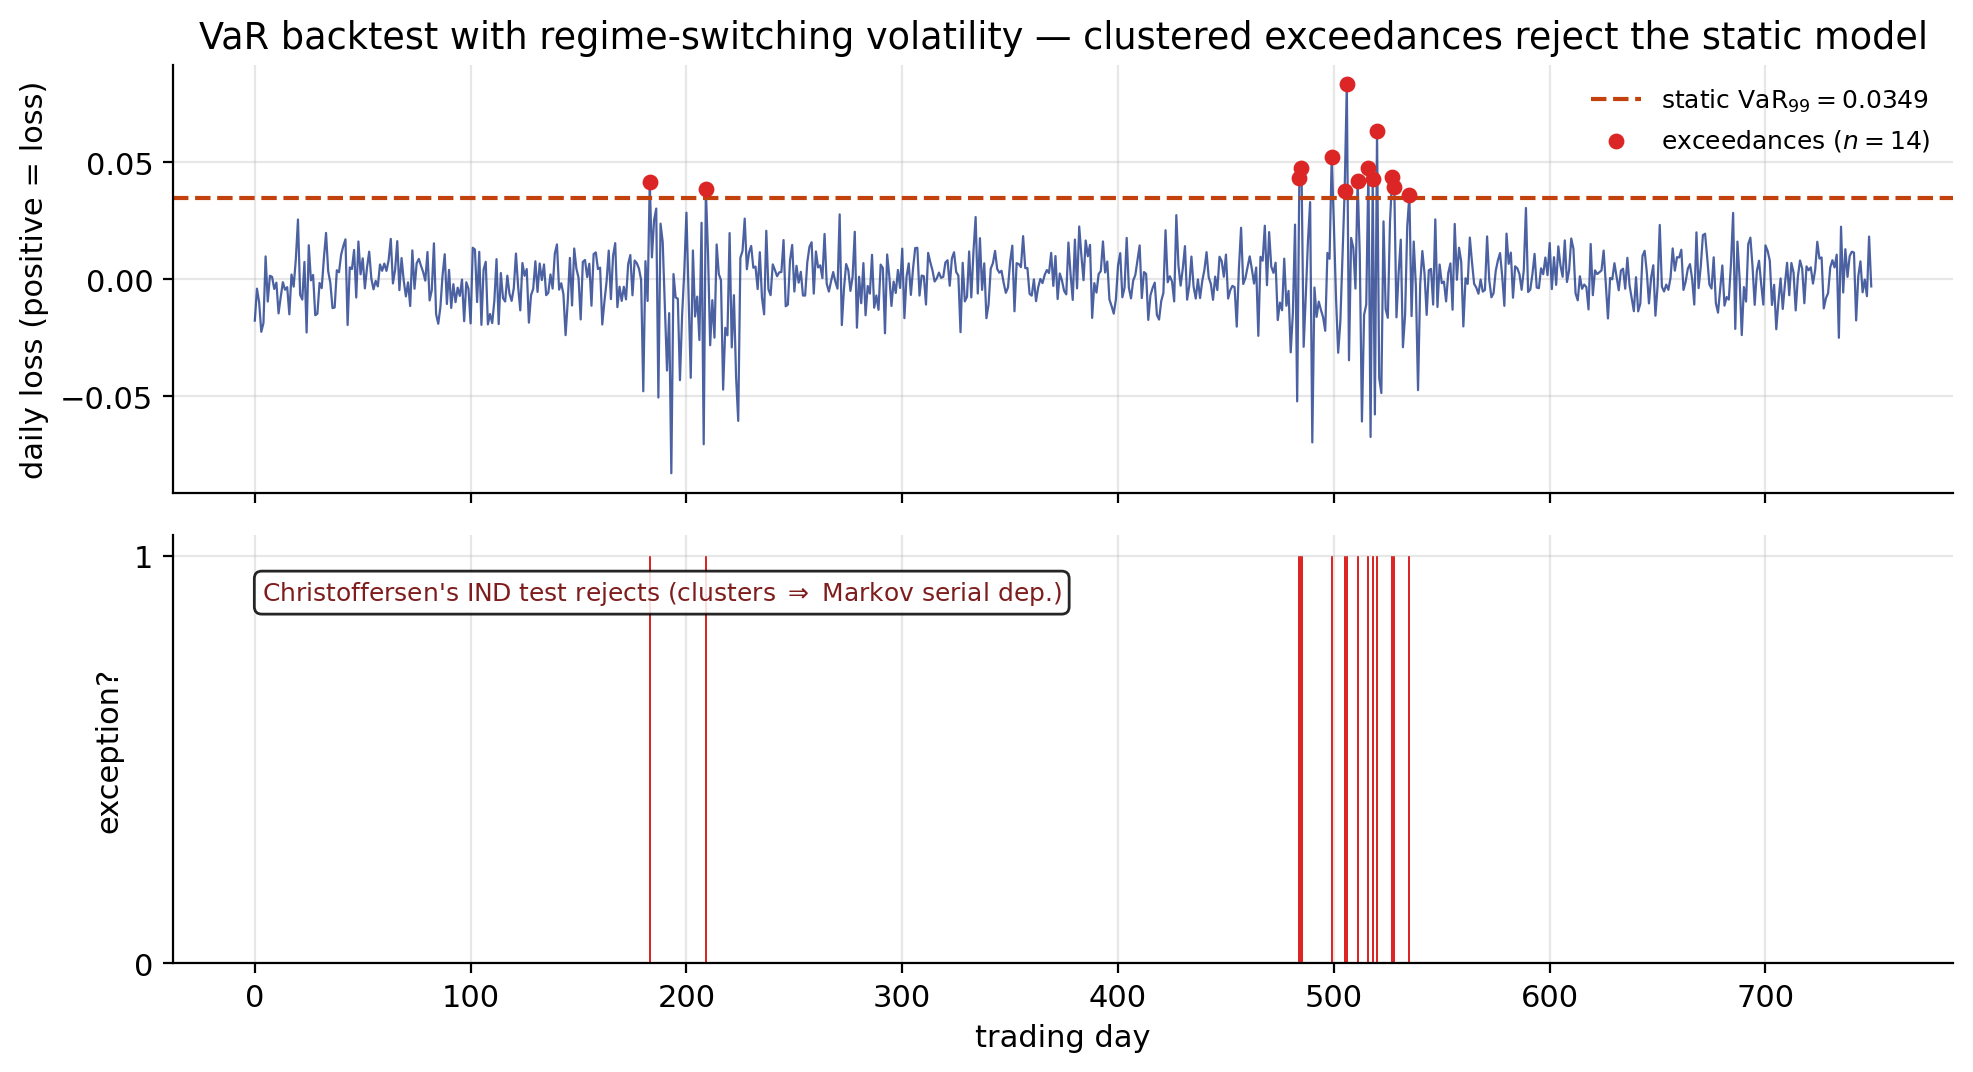
\includegraphics[keepaspectratio]{figures/ch15-backtest-clustering.png}}
\caption{Daily losses with a static 99\% VaR line, exceedances marked
red --- clustered in two stressed windows. Christoffersen's IND test
rejects on clustering even when total count is in-range. Exactly the
failure mode that flagged static-vol VaR models during March 2020 and
the 2022 rates regime change}
\end{figure}

\subsection{15.7.3 Christoffersen's independence
test}\label{christoffersens-independence-test}

Kupiec catches miscalibrated levels but misses \emph{clustering} --- a
model whose exceedances come bunched together in crisis periods and
sparse elsewhere, so the overall count looks right but the temporal
pattern is wrong. Clustering indicates the model fails to capture
volatility dynamics: on Monday the model reports a VaR that was
appropriate for last week's calm conditions, the market blows out,
Tuesday's VaR is still calibrated to last week, Wednesday the same, and
suddenly you have four exceedances in four days because the dynamic
volatility of the market was not reflected in the dynamic VaR of the
model.

Christoffersen's test models the exceedance sequence as a two-state
Markov chain. Let \(n_{ij}\) be the count of transitions from state
\(i\) to state \(j\) (where 0 = no exceedance, 1 = exceedance). Under
independence, the transition probability
\(\mathbb{P}(I_t = 1 \mid I_{t-1} = 1)\) equals the unconditional
\(\mathbb{P}(I_t = 1) = \alpha\). The likelihood-ratio test against a
general Markov alternative is

\[
\mathrm{LR}_{\mathrm{IND}} \;=\; -2 \log\!\left[\frac{\hat{p}^{x}(1 - \hat{p})^{n - x}}{\hat{p}_{01}^{n_{01}}(1 - \hat{p}_{01})^{n_{00}} \hat{p}_{11}^{n_{11}}(1 - \hat{p}_{11})^{n_{10}}}\right] \sim \chi^2_1, \tag{15.14}
\]

where \(\hat{p}_{i1} = n_{i1}/(n_{i0} + n_{i1})\). Combined with Kupiec,
the \emph{conditional coverage} test

\[
\mathrm{LR}_{\mathrm{CC}} \;=\; \mathrm{LR}_{\mathrm{POF}} + \mathrm{LR}_{\mathrm{IND}} \;\sim\; \chi^2_2 \tag{15.15}
\]

rejects the model if either the overall frequency is wrong or the
clustering is significant, giving a comprehensive test of VaR adequacy.
A failing \(\mathrm{LR}_{\mathrm{IND}}\) with passing
\(\mathrm{LR}_{\mathrm{POF}}\) is a characteristic signature of a model
using a slow-moving volatility estimator (rolling 1-year window, for
example) in a market with pronounced vol clustering --- the fix is
typically to move to a GARCH-type conditional-volatility specification.

\subsection{15.7.4 Backtesting CTE}\label{backtesting-cte}

CTE backtesting is considerably harder because CTE is not elicitable
(§15.3). The simplest approach --- and the one adopted in FRTB --- is to
backtest CTE indirectly by backtesting VaR at multiple confidence levels
(typically 97.5\% and 99\%) and examining the distribution of exceedance
magnitudes. A model whose VaR is correctly calibrated at both 97.5\% and
99\% is approximately correctly calibrated for CTE at 97.5\%, because
CTE is approximately an average over the range between those quantiles.

The \emph{Acerbi-Szekely} framework proposes scoring functions for joint
VaR/CTE backtesting. Three families of tests are commonly implemented:
(i) a test on the magnitude of exceedances (the average exceedance
should match the CTE minus VaR prediction); (ii) a test on the
tail-conditional distribution of \(L\) relative to the model's predicted
tail distribution (a sort of Kolmogorov-Smirnov test in the tail); (iii)
a joint test on the first two moments of the exceedance distribution.
These are more complex to implement but increasingly standard in banks'
model-validation departments.

Practical note: CTE backtests have low statistical power unless the data
history is long. On a 1-year backtest at 99\% confidence, there are only
2-3 expected exceedances --- essentially no usable information about the
conditional expectation of the tail. Meaningful CTE backtests require
3-5 year histories or pooling across multiple portfolios, which is why
the FRTB compromise of backtesting VaR at two levels and inferring CTE
adequacy has dominated implementation.

The broad lesson: backtesting is as much a research area as a compliance
exercise. Every risk measure has its own backtesting theory, and
practitioners must choose tests that match the quantity being
backtested, recognise the limitations of finite-sample power, and
interpret results as diagnostic rather than purely pass/fail.

\section{15.8 Stress Testing}\label{stress-testing}

Stress testing sits alongside VaR/CTE as the second major pillar of
market-risk measurement. The premise is that statistical models
calibrated on historical data fail precisely when history fails to
contain the next catastrophe --- so one should also ask ``what if the
stock market falls 30\% in a week?'' or ``what if credit spreads widen
to 2008 levels?'' regardless of what the statistical model predicts.

\subsection{15.8.1 Historical stress
scenarios}\label{historical-stress-scenarios}

\emph{Historical stress scenarios} replay a specific historical event
against the current portfolio, applying the market moves from that
period as instantaneous shocks. Canonical scenarios include Black Monday
1987, the Asian Crisis 1998, LTCM autumn 1998, the Dot-Com crash of
2000-2001, Lehman September 2008, the Flash Crash of May 2010, the
EuroZone sovereign crisis 2011-2012, the China devaluation of August
2015, Volmageddon in February 2018, the COVID-19 crash of March 2020,
and the UK gilt crisis of September-October 2022.

The appeal of historical scenarios is that they are ``real'': everyone
agrees that Lehman happened, and there is no arguing about the size of
the moves. The limitation is that the next crisis will not be the last
crisis; hedging against 2008 may not protect against a different
structural breakdown. Every historical scenario also requires
translation to today's portfolio --- one cannot just apply 1987 S\&P
moves verbatim to today's equity book because today's book contains
index futures that did not exist in 1987, options markets whose implied
vol surface is unrecognisable from that era, and hedging relationships
that behave differently under modern market microstructure. The
translation introduces modelling judgement, and different risk teams
make different calls.

\subsection{15.8.2 Hypothetical stress
scenarios}\label{hypothetical-stress-scenarios}

\emph{Hypothetical stress scenarios} are designed by the risk committee
to capture imagined but not-yet-realised catastrophes. Examples:
``equity down 25\%, vol up to 80, credit spreads +500 bp, USD up 10\%,
oil down 40\%''; ``Treasury yields rise 300 bp in a week''; ``Bitcoin
goes to zero overnight, dragging the tech-heavy NASDAQ down 15\% on
correlation contagion.'' These scenarios reflect institutional views
about what could go wrong and stress the risks that are \emph{not} in
the historical record.

Regulatory stress tests --- CCAR in the US, EBA stress tests in the EU,
Bank of England stress tests in the UK --- are hypothetical scenarios
imposed on all banks simultaneously, with the bank having to show that
its capital remains above regulatory minima even under the imposed
stress. These exercises combine a macroeconomic narrative (unemployment
rises 5 points, GDP contracts 3\%, house prices fall 25\%) with specific
market-variable shocks implied by the narrative, and force banks to
project their balance sheet, P\&L, and capital ratio through the stress
horizon (typically 9 quarters).

\subsection{15.8.3 Reverse stress testing}\label{reverse-stress-testing}

A third variety, increasingly emphasised by regulators, is \emph{reverse
stress testing}: rather than starting with a scenario and computing the
loss, start with a loss (typically the failure threshold --- the loss
that would render the firm insolvent or non-viable) and work backward to
identify scenarios that produce it. The output is not a capital number
but a catalogue of scenarios whose realisation would destroy the firm,
some of which may be obvious and others of which may surprise the risk
committee.

Reverse stress testing is mathematically harder than forward stress
because there are many scenarios that produce a given total loss --- the
problem is an inverse problem with a large null space. Practical
implementations typically constrain the scenario space by factor
structure (what combinations of factor shocks within 5 standard
deviations produce failure?) or by qualitative narrative (what operating
environments plausibly produce the shocks that produce failure?).

\subsection{15.8.4 Scenario construction
methodology}\label{scenario-construction-methodology}

Building useful stress scenarios is its own craft. Core principles:

\begin{itemize}
\tightlist
\item
  \emph{Internal consistency.} A scenario must be coherent across
  markets. An equity-down scenario usually has vol up, credit spreads
  wider, and safe-haven currencies (CHF, JPY, USD) stronger. Applying an
  equity-down shock in isolation without these co-moves gives an
  artificially small loss and misses the real tail risk.
\item
  \emph{Magnitude calibration.} Shocks should be large enough to matter
  but not so large as to be dismissed as absurd. A 20-sigma equity move
  on a Normal calibration is absurd but on a Student-\(t_3\) calibration
  it is a routine crisis move. Calibrating shock sizes to fat-tailed
  distributions gives more credibility and more informative stress
  results.
\item
  \emph{Coverage of risk types.} The scenario suite should collectively
  exercise every risk factor the book is exposed to --- not just the
  obvious ones. A scenario suite that stresses equity and rates but
  ignores FX, credit, vol, and correlation leaves systematic gaps.
\item
  \emph{Narrative plausibility.} Senior management engages with stress
  tests that come with a story (``oil price shock triggers recession,
  which triggers credit widening, which forces unwinds in levered funds,
  which cascades back into equities''). Pure statistical shocks without
  narrative are harder to action.
\end{itemize}

\subsection{15.8.5 Economic capital and solvency
horizons}\label{economic-capital-and-solvency-horizons}

\emph{Economic capital} is the amount of capital the firm's internal
models say is needed to remain solvent over a specified horizon
(typically 1 year) at a specified confidence level (typically 99.9\% ---
a 1-in-1000 year event). Economic capital differs from regulatory
capital in several ways: it uses the firm's own modelling framework (not
the regulator's), it runs at a much longer horizon and higher confidence
level, and it aggregates across all risk types (market, credit,
operational, business, strategic) whereas regulatory market-risk capital
concerns only market risk. Economic capital is the basis for internal
return-on-capital calculations, ratings-agency assessments, and internal
reinsurance or capital-transfer decisions.

The relationship between stress testing and VaR/CTE is subtle. VaR/CTE
report the \emph{expected} catastrophe based on an assumed distribution;
stress tests report a \emph{specific} catastrophe imagined or observed.
They are complementary, not substitutes. A portfolio with low VaR can
have large stress P\&L (vulnerable to a specific imagined scenario
outside the historical record), and vice versa. A mature risk function
reports both, and uses significant discrepancies between them as a
diagnostic for hidden non-linearity or for over-reliance on a particular
set of historical data.

\section{15.9 Risk Decomposition}\label{risk-decomposition}

Once an aggregate VaR or CTE has been computed, the operational question
is ``which positions contribute to it, and by how much?'' This is the
\emph{risk-decomposition} problem, and it has three principal answers:
marginal, component, and incremental. Each answers a slightly different
question, and a well-run risk function reports all three.

\subsection{15.9.1 Marginal VaR}\label{marginal-var}

\emph{Marginal VaR} of a position is the partial derivative of portfolio
VaR with respect to the position size. It answers: if I add one more
dollar of exposure to this position, how much does my VaR go up? Under
the delta-normal model with portfolio volatility
\(\sigma_P = \sqrt{w^{\top} \Sigma w}\), the marginal VaR of position
\(i\) is

\[
\mathrm{mVaR}_i \;=\; \frac{\partial \mathrm{VaR}}{\partial w_i} \;=\; z_{1-\alpha}\,\frac{(\Sigma w)_i}{\sigma_P}, \tag{15.16}
\]

where \((\Sigma w)_i\) is the covariance of position \(i\)'s return with
the portfolio return. Marginal VaR is natural for incremental trade
decisions --- it directly measures the risk impact of adding a little
more of something. Sign is informative: a position with negative
marginal VaR \emph{reduces} portfolio risk when added (it is a net
hedge), and the risk team should be happy to see it grow.

\subsection{15.9.2 Component VaR}\label{component-var}

\emph{Component VaR} is the contribution of a position to the portfolio
VaR, obtained via Euler allocation:

\[
\mathrm{cVaR}_i \;=\; w_i \cdot \mathrm{mVaR}_i, \qquad \sum_i \mathrm{cVaR}_i \;=\; \mathrm{VaR}. \tag{15.17}
\]

The additive property is the key. Component VaRs sum to the total, which
makes component VaR the natural basis for risk-budget allocation ---
each desk is given a budget, and the sum of desk-level VaRs equals
firm-level VaR without residual. Under the delta-normal framework,
component VaR is proportional to the position's covariance with the
portfolio, scaled by portfolio size. Euler allocation generalises to any
positively homogeneous risk measure, including CTE, so component CTE is
defined analogously and sums exactly to portfolio CTE.

\subsection{15.9.3 Incremental VaR}\label{incremental-var}

\emph{Incremental VaR} of a position is the change in portfolio VaR if
the position is removed entirely:

\[
\mathrm{iVaR}_i \;=\; \mathrm{VaR}(\text{full portfolio}) - \mathrm{VaR}(\text{portfolio without position } i). \tag{15.18}
\]

It is a finite-difference rather than an infinitesimal measure, and for
large positions can differ significantly from component VaR. Incremental
VaR is natural for unwind decisions --- it directly measures ``how much
risk do I free up if I close this position today?'' For small positions,
incremental VaR and component VaR agree; for large positions (especially
those with non-linear P\&L), they diverge by factors of 2 or more.
Incremental VaRs do not generally sum to the total, because removing one
position changes the risk impact of every other position through the
correlation matrix.

\subsection{15.9.4 A worked contrast}\label{a-worked-contrast}

Consider a portfolio consisting of a long stock position and a short
call on the same stock --- a covered call. Suppose the stock has
component VaR \$1M and the short call has component VaR \$0.3M, summing
to \$1.3M. But if we remove just the stock, the short call alone has VaR
\$0.6M --- the incremental VaR of removing the stock is \$0.7M. If we
remove just the short call, the long stock alone has VaR \$1.2M --- the
incremental VaR of removing the call is \$0.1M. The differences reflect
the hedging interaction between the two positions: each individually is
riskier than its contribution to the pair because each partially hedges
the other. The three attributions answer three different questions, and
a risk team that reports only one is depriving its traders of meaningful
optionality in trade sizing and unwind sequencing.

\subsection{15.9.5 Non-linear portfolios and CTE
decomposition}\label{non-linear-portfolios-and-cte-decomposition}

For portfolios with significant non-linearity (options, convertibles,
structured products), the delta-normal formulas above are a first
approximation. The Euler-allocation framework extends to CTE and to
Monte-Carlo-based risk measures under mild regularity: if \(\rho\) is a
positively homogeneous risk measure and the portfolio is parameterised
by weights \(w\), then

\[
\rho(w) \;=\; \sum_i w_i \frac{\partial \rho}{\partial w_i}(w), \tag{15.19}
\]

and \(w_i \partial \rho / \partial w_i\) is the component contribution
of position \(i\). For a Monte Carlo CTE, the component contribution of
a position can be estimated by running the simulation with and without
an incremental position, or --- more efficiently --- by computing the
conditional expectation of the position's P\&L given that the portfolio
is in the tail.

Risk decomposition answers the fundamental governance question ``where
does my risk come from?'' Pairing it with the P\&L attribution discussed
next closes the loop between pre-trade forecasts and post-trade
realisations.

\section{15.10 P\&L Attribution}\label{pl-attribution}

A sibling discipline to risk decomposition is \emph{P\&L attribution}:
after the trading day closes, decompose the realised P\&L into
contributions from each Greek and each market move. A canonical
Greek-based attribution for a derivatives book reads

\[
\Delta V \;=\; \delta \cdot \Delta S + \tfrac{1}{2} \Gamma (\Delta S)^2 + \nu \cdot \Delta \sigma + \theta \cdot \Delta t + \rho \cdot \Delta r + \text{cross-Greeks} + \text{cash flows} + \text{residual}, \tag{15.20}
\]

where \(\delta, \Gamma, \nu, \theta, \rho\) are the book's Greeks (see
Chapter 7 for definitions) and
\(\Delta S, \Delta \sigma, \Delta t, \Delta r\) are the realised moves
in spot, implied vol, time, and rates. The ``cross-Greeks'' bucket
collects contributions from vanna (spot-vol cross-gamma), volga
(vol-of-vol), charm (spot-time), and speed (third-order in spot); the
``cash flows'' bucket captures discrete events such as dividends,
coupons, and realised trade P\&L from intra-day executions.

The ``residual'' --- the piece the model cannot explain --- is the
diagnostic. It should be small. A systematically large residual is a red
flag that either the Greeks are mis-computed, the book contains
instruments not captured by the risk model, or the market moves include
components (a basis dislocation, a vol-surface reshaping, a correlation
break) that the factor representation does not span.

\subsection{15.10.1 Hypothetical, risk-theoretical, and actual P\&L
(FRTB PLA)}\label{hypothetical-risk-theoretical-and-actual-pl-frtb-pla}

FRTB (BCBS d352) formalises attribution into the \emph{P\&L attribution
test}. Three P\&L series are produced each day:

\begin{itemize}
\tightlist
\item
  \emph{Actual P\&L} --- the realised P\&L from the trading systems,
  including intra-day trading and any accruals the risk model doesn't
  capture.
\item
  \emph{Hypothetical P\&L} --- the front-office full-revaluation P\&L on
  the \emph{frozen} end-of-day positions under the day's \emph{actual}
  market moves. No intra-day trading; the book is repriced by the full
  pricing library using the realised end-of-day market data. This is the
  ``what the front-office price says the frozen book earned''.
\item
  \emph{Risk-theoretical P\&L} --- the \emph{risk-engine}
  full-revaluation P\&L on the same frozen positions under the
  \emph{risk model's} representation of the day's market data (the
  limited set of risk factors the model actually carries). This is the
  ``what the risk engine, restricted to its own risk-factor set, says
  the frozen book earned''.
\end{itemize}

The PLA test compares the \emph{hypothetical} and
\emph{risk-theoretical} series, measuring the Spearman correlation and a
KS-statistic on their differences; the desk passes (and may keep using
its internal model) only if both metrics stay inside the BCBS
thresholds. Failing forces a switch to the Standardised Approach, which
typically carries materially higher capital. The Taylor-via-Greeks
expression in (15.20) is \emph{Greek-attributed} P\&L --- useful as an
internal diagnostic, but distinct from the risk-theoretical series the
regulator examines.

\subsection{15.10.2 Attribution disputes and model-maintenance
signals}\label{attribution-disputes-and-model-maintenance-signals}

In practice, attribution is where traders and risk managers spend a
great deal of time talking past each other. The trader's P\&L report
(from the front-office system) and the risk desk's P\&L report (from the
risk engine) will rarely agree to the last dollar --- and when they
disagree by a material amount, the question is which number to believe.
Some differences are legitimate and bookkeepable (FX conversion rates,
intraday funding, stale prices); others are diagnostic of a genuine
model-data problem (a mispriced exotic, an ignored correlation).

A systematic pattern in the residual is the most valuable piece of
information attribution provides. If the residual is consistently
positive on up-days and negative on down-days, the risk model is missing
a positive gamma exposure somewhere. If the residual is systematically
negative near expiry for positions that are being managed to zero, the
risk model's decay profile is wrong. If the residual explodes on days
with large vol moves, the vega or volga computation is suspect. Treating
attribution residual as pure noise misses the diagnostic signal and lets
model errors compound unnoticed.

\subsection{15.10.3 Greek decomposition versus factor
decomposition}\label{greek-decomposition-versus-factor-decomposition}

Two complementary views of attribution are common. \emph{Greek
decomposition} expresses P\&L as in (15.20) --- one term per Greek,
times the corresponding market move. \emph{Factor decomposition}
expresses P\&L as a sum over underlying risk factors, each factor
contributing its net movement against the book's net sensitivity. The
two views are mathematically related (a Greek on a derivative is the
sensitivity to the factor that drives the derivative) but
organisationally distinct: Greek decomposition is natural for a
derivatives trader thinking about hedging; factor decomposition is
natural for a portfolio manager thinking about exposures and hedges
across asset classes.

Together, risk decomposition (pre-trade, ``how much risk does this
add?'') and P\&L attribution (post-trade, ``where did the P\&L come
from?'') form the bookends of a complete risk-management cycle. The
pre-trade forecast and the post-trade realisation should agree on
average and diverge only within known bounds; when they diverge outside
those bounds, the discrepancy triggers either a trading adjustment (the
book is doing something the traders did not intend) or a model revision
(the risk framework is missing something).

\section{15.11 Liquidity-Adjusted Risk}\label{liquidity-adjusted-risk}

The classical VaR/CTE framework assumes that positions can be liquidated
at mid-market prices with no market impact over the VaR horizon. This
assumption breaks down for illiquid instruments --- distressed credit,
emerging-market equities, complex structured products --- where selling
in a hurry carries material bid-ask cost or even an inability to
transact at any price.

\subsection{15.11.1 Exogenous liquidity
cost}\label{exogenous-liquidity-cost}

The simplest form of liquidity adjustment adds a fixed bid-ask haircut
to the VaR:

\[
\mathrm{LVaR}_\alpha \;=\; \mathrm{VaR}_\alpha + \tfrac{1}{2}\,|w| \cdot \mathrm{spread}, \tag{15.21}
\]

where \(|w|\) is the absolute position size and ``spread'' is the
bid-ask spread as a fraction of mid. The factor of one-half reflects
that half the spread is the cost of liquidating (selling at the bid from
mid) and the other half is the cost of re-entering if the position is
repurchased. More refined versions add a term for the \emph{volatility
of the spread} itself --- widening bid-ask in stressed markets --- by
treating the spread as a random variable and adding a quantile of its
distribution to the VaR.

\subsection{15.11.2 Endogenous market
impact}\label{endogenous-market-impact}

For large positions in any market, the act of liquidating moves prices.
The simplest model is a square-root market-impact law: the price impact
of unwinding \(Q\) shares over a horizon \(h\) is approximately
\(k \sigma \sqrt{Q / (V h)}\), where \(V\) is average daily volume and
\(k\) is an asset-class-specific constant (0.5-1.5 typical for
equities). Incorporating this into VaR adds a market-impact charge that
scales non-linearly with position size, capturing the economic reality
that doubling a position more than doubles the unwind cost.

\subsection{15.11.3 Liquidity horizons in
FRTB}\label{liquidity-horizons-in-frtb}

FRTB institutionalises liquidity adjustment by prescribing
\emph{liquidity horizons} by asset class rather than computing bid-ask
directly. The idea is to capture the extended period of price exposure
during an assumed unwind rather than the instantaneous cost:

\begin{itemize}
\tightlist
\item
  10 days: major currencies, large-cap equities, interest rates in G10
  currencies.
\item
  20 days: emerging-market FX and sovereigns, small-cap equities.
\item
  40 days: investment-grade corporate credit.
\item
  60 days: high-yield corporate credit, structured products.
\item
  120 days: exotic credit, private-equity-like structured positions.
\end{itemize}

Capital for an instrument is computed as a 10-day ES times a liquidity
adjustment that scales with the horizon. The formula is constructed so
that positions with longer liquidity horizons accumulate capital
proportional to their extended exposure. An illiquid corporate bond
whose prescribed liquidity horizon is 60 days carries six times the
exposure window of a liquid equity and correspondingly higher capital.

\subsection{15.11.4 Funding liquidity
risk}\label{funding-liquidity-risk}

\emph{Funding liquidity} --- the risk that the firm cannot finance its
positions at a reasonable cost --- is managed separately via LCR, NSFR,
and stress analyses, but interacts with market risk in crises (liquidity
shock \(\to\) forced unwinds \(\to\) price moves \(\to\) further margin
calls). The Lehman collapse of September 2008 and the COVID liquidity
crunch of March 2020 both featured this doom-loop, and the AAA-rated
corporates trading at 70 cents on the dollar in March 2020 were not
credit-impaired --- they were leverage-impaired. Single-instrument VaR
cannot easily capture emergence; this is what the FRTB NMRF charge and
stress scenarios try to address.

\section{15.12 Delta-Gamma Parametric
VaR}\label{delta-gamma-parametric-var}

The delta-gamma framework (see Chapter 7 for the derivation of the
Greeks themselves) delivers a specific computational payoff:
\emph{delta-gamma parametric VaR}. This technique was the workhorse of
risk systems in the 1990s and 2000s and remains important today as a
fast first-pass estimate even when full revaluation is available. It is
a concrete application of the quadratic Taylor expansion of book P\&L
combined with the Cornish-Fisher expansion of §15.2.

\subsection{15.12.1 The quadratic
approximation}\label{the-quadratic-approximation}

For a portfolio of options and hedges on \(n\) risk factors
\(r = (r_1, \ldots, r_n)\), expand the portfolio value \(V(r)\) to
second order around the current factor vector \(r_0\):

\[
\Delta V(r) \;\approx\; \delta^{\top}\,\Delta r + \tfrac{1}{2}\,\Delta r^{\top}\,\Gamma\,\Delta r, \tag{15.22}
\]

where \(\delta_i = \partial V / \partial r_i\) and
\(\Gamma_{ij} = \partial^2 V / \partial r_i \partial r_j\) evaluated at
\(r_0\). For an equity option book, \(r\) includes spots, implied vols,
and rates; \(\delta\) collects the deltas, vegas, and rhos; and
\(\Gamma\) collects the gammas, vannas, volgas, and cross-sensitivities.
The approximation is accurate for moderate factor moves and degrades for
very large moves where cubic and higher-order terms matter.

\subsection{15.12.2 Moments of the quadratic form under Normal
factors}\label{moments-of-the-quadratic-form-under-normal-factors}

Assume \(\Delta r \sim \mathcal{N}(0, \Sigma)\) with covariance matrix
\(\Sigma\). The quadratic form has a closed-form mean, variance, and
higher moments. The first two are

\[
\mu_P \;=\; \mathbb{E}[\Delta V] \;=\; \tfrac{1}{2}\,\mathrm{tr}(\Gamma \Sigma), \tag{15.23}
\]

\[
\sigma_P^2 \;=\; \mathrm{Var}[\Delta V] \;=\; \delta^{\top} \Sigma\,\delta + \tfrac{1}{2}\,\mathrm{tr}((\Gamma \Sigma)^2). \tag{15.24}
\]

The mean is non-zero whenever \(\Gamma\) is non-zero: a long-gamma book
has positive expected P\&L from the gamma convexity even under zero-mean
factor moves, and vice versa for a short-gamma book. The variance has a
linear-sensitivity piece \(\delta^{\top} \Sigma \delta\) (the
delta-normal term) plus a quadratic-sensitivity piece
\(\frac{1}{2} \mathrm{tr}((\Gamma \Sigma)^2)\) (the gamma contribution).

The third and fourth central moments of \(\Delta V\), used for
Cornish-Fisher, are

\[
m_3 \;=\; 8\,\mathrm{tr}((\Gamma \Sigma)^3) + 6\,\delta^{\top} \Sigma\,\Gamma\,\Sigma\,\delta, \tag{15.25}
\]

\[
m_4 \;=\; 12\,\mathrm{tr}((\Gamma \Sigma)^4) + 48\,\delta^{\top}(\Sigma\Gamma)^2 \Sigma\,\delta + 3\,(\sigma_P^2)^2. \tag{15.26}
\]

Both expressions follow from the eigen-decomposition of
\(\Sigma^{1/2}\Gamma\Sigma^{1/2}\), under which the quadratic form
becomes a weighted sum of independent chi-squared random variables and
arbitrary moments follow from sums over the eigenvalues.

\subsection{15.12.3 Cornish-Fisher VaR}\label{cornish-fisher-var}

Feed the standardised skewness \(s = m_3 / \sigma_P^3\) and excess
kurtosis \(\kappa = m_4 / \sigma_P^4 - 3\) into the Cornish-Fisher
expansion (15.4):

\[
\mathrm{VaR}_\alpha \;\approx\; -\mu_P + \sigma_P \left[ z_\alpha + \tfrac{1}{6}(z_\alpha^2 - 1)\,s + \tfrac{1}{24}(z_\alpha^3 - 3 z_\alpha)\,\kappa \right]. \tag{15.27}
\]

The whole computation is \(O(n^2)\) in the number of risk factors for
the moment evaluation and \(O(1)\) for the Cornish-Fisher adjustment ---
much cheaper than a full Monte Carlo revaluation. A portfolio with 500
risk factors and 10,000 options can have its delta-gamma-Cornish-Fisher
VaR computed in under a second on a modern workstation; a full Monte
Carlo revaluation of the same portfolio might take minutes or hours
depending on the sophistication of the option pricers. The speed
differential is the reason delta-gamma VaR survives even in the
full-revaluation era: it is what the intraday risk engine runs, while
the overnight batch runs the full Monte Carlo.

\subsection{15.12.4 Accuracy regime}\label{accuracy-regime}

The accuracy of delta-gamma VaR depends on the magnitude of the stress
move relative to the curvature of the payoff:

\begin{itemize}
\tightlist
\item
  \emph{Daily 95\% VaR, moderate vol.} The approximation is typically
  within a few percent of a full-revaluation VaR. Perfectly adequate for
  intraday limit monitoring and desk-level reporting.
\item
  \emph{Daily 99\% VaR, stressed conditions.} Accuracy degrades to
  5-15\% typical error. Still useful as a first-pass indicator but
  should be validated against full revaluation before being used for
  capital.
\item
  \emph{10-day 99\% VaR with options near expiry.} Can degrade severely
  because near-expiry gamma is explosive and the quadratic approximation
  misses third-order effects. Full revaluation or Monte Carlo is
  mandatory here.
\item
  \emph{Deeply out-of-the-money options or digital-like payoffs.}
  Delta-gamma breaks down entirely because the payoff is nearly
  discontinuous. Full revaluation is required.
\end{itemize}

Modern risk systems run delta-gamma-Cornish-Fisher VaR for intraday risk
updates and full-revaluation Monte Carlo VaR for end-of-day reporting,
taking advantage of the speed of the former and the accuracy of the
latter. When the two disagree by more than a threshold, the system flags
a review.

\subsection{15.12.5 Moment-matching
variants}\label{moment-matching-variants}

A refinement of Cornish-Fisher is \emph{moment matching}: fit a
parametric distribution (e.g.~a mixture of Normals, a Johnson curve, or
a shifted log-Normal) whose first four moments match the closed-form
moments \(\mu_P, \sigma_P^2, m_3, m_4\) of the quadratic form. The
quantile of the fitted distribution is taken as the VaR. Moment matching
avoids the non-monotonicity problems of Cornish-Fisher at extreme
parameter values and tends to be more accurate for moderately skewed
distributions. The cost is a slightly more elaborate implementation ---
the fitting step is not purely closed-form --- and in practice
Cornish-Fisher and moment-matching give very similar answers except in
pathological cases.

An alternative to both is \emph{Imhof's method}: numerically invert the
characteristic function of the quadratic form to recover the full
distribution of \(\Delta V\), then take the exact quantile. Imhof is
more accurate than Cornish-Fisher but computationally heavier and is
typically reserved for end-of-day validation runs rather than intraday
computation. The progression Delta-Normal → Delta-Gamma-Cornish-Fisher →
Imhof → full Monte Carlo represents a ladder of increasing accuracy and
increasing computational cost, with the risk team picking the
appropriate rung for each use case.

\subsection{15.12.6 Operational role}\label{operational-role}

Delta-gamma parametric VaR is not merely a back-pocket approximation. In
the modern risk stack it plays several distinct roles:

\begin{itemize}
\tightlist
\item
  \emph{Intraday limit monitoring.} When a trader executes a new option
  trade, the risk system can refresh the desk's VaR in milliseconds
  using the delta-gamma approximation. Full revaluation is too slow for
  this use case.
\item
  \emph{Sensitivity of VaR to positions.} Because the moment inputs
  \((\mu_P, \sigma_P, s, \kappa)\) of (15.27) are themselves smooth
  functions of \(\delta\), \(\Gamma\), and the factor covariance
  \(\Sigma\), the formula is differentiable through to
  \(\delta, \Gamma\), and the marginal VaR (§15.9) of any prospective
  trade can be computed in closed form. This supports pre-trade
  ``what-if'' analysis without running Monte Carlo for every candidate
  trade.
\item
  \emph{Regulatory backup.} If a bank's full-revaluation Monte Carlo
  engine fails or times out, the delta-gamma approximation provides a
  fallback VaR that can be used to continue limit monitoring and
  regulatory reporting while the primary engine is repaired.
\end{itemize}

Cross-reference: the Greeks \(\delta\) and \(\Gamma\) used here are the
multi-factor generalisations of the scalar deltas and gammas developed
in Chapter 7. The single-name case \(n = 1\) of (15.22) reduces exactly
to the scalar delta-gamma expansion around the Black-Scholes price.

\section{15.13 Hedged P\&L Distribution and Hedged
CTE}\label{hedged-pl-distribution-and-hedged-cte}

The input to a VaR calculation for an options desk is the \emph{hedged}
P\&L distribution, not the unhedged P\&L distribution. Hedging reshapes
the underlying factor moves into a residual P\&L that the desk actually
experiences; the risk measure then quantifies the tail of that residual.
Hedging decisions and risk-measurement decisions are therefore coupled:
a tighter hedge means a smaller residual, which means a smaller VaR,
which means lower capital consumption. Conversely, a looser hedge means
larger residuals and higher capital. The CFO and the CRO have aligned
interests in encouraging tight hedging, subject to the caveat that
over-hedging generates transaction-cost bleed that itself shows up in
P\&L.

\subsection{15.13.1 The shape of residual hedged
P\&L}\label{the-shape-of-residual-hedged-pl}

Consider an option position \(f(t, S_t)\) hedged with \(\alpha_t\)
shares and \(\beta_t\) units of money-market account, rebalanced on a
grid \(t_0 < t_1 < \ldots < t_N\). Between rebalance times the hedge is
stale, and the residual P\&L increment over interval \((t_{k-1}, t_k)\)
is, to leading order,

\[
\Delta R_k \;\approx\; \tfrac{1}{2}\,\Gamma(t_{k-1}, S_{t_{k-1}}) \cdot (S_{t_k} - S_{t_{k-1}})^2 - \theta(t_{k-1}, S_{t_{k-1}}) \cdot \Delta t. \tag{15.28}
\]

This is the celebrated Taylor-series identity at the heart of dynamic
hedging (see Chapter 7 for the full derivation): the gamma-convexity
term pays the holder whenever spot moves, and the theta-decay term
charges the holder for the option's time decay. On average, under GBM
with the Black-Scholes vol and frictionless rebalancing, the two exactly
cancel --- that is the content of the replication theorem. In practice,
the cancellation is imperfect at every finite rebalance frequency, and
the imperfection is the residual P\&L.

The distribution of total hedged P\&L over the option's life is
approximately Gaussian for sufficiently fine rebalancing (by a
central-limit argument across the sum of increments) with variance
proportional to \(1/N\) where \(N\) is the number of rebalance steps.
More frequent rebalancing gives tighter hedged P\&L. This is the source
of the scaling law in §15.13.2 below.

\subsection{15.13.2 Delta versus delta-gamma hedging and CTE
reduction}\label{delta-versus-delta-gamma-hedging-and-cte-reduction}

The CTE of a hedged book is typically much smaller than the CTE of the
unhedged book, but the reduction ratio depends on whether the hedge is
first- or second-order. Rough scaling:

\begin{itemize}
\tightlist
\item
  \emph{Delta-only hedge} reduces residual variance by a factor of
  approximately \(\sigma^2 \Delta t\) per rebalance step. Cumulatively
  over the life of an option with daily rebalancing, this translates to
  CTE reductions of 70-90\% relative to the unhedged position.
\item
  \emph{Delta-gamma hedge} (using a second traded option to neutralise
  gamma) reduces residual variance by another factor of approximately
  \(\sigma^2 \Delta t\), giving CTE reductions of 95-99\% relative to
  the unhedged position at realistic daily rebalance frequencies.
\end{itemize}

The gamma hedge squeezes the residual P\&L into the third-order Taylor
remainder, which scales as \((\Delta S)^3\) rather than
\((\Delta S)^2\). Since \(\Delta S \sim \sigma S \sqrt{\Delta t}\), the
cube is of order \(\sigma^3 S^3 \Delta t^{3/2}\), which is much smaller
than the square \(\sigma^2 S^2 \Delta t\) for small \(\Delta t\). Each
additional Greek matched reduces the hedging residual by another power
of \(\sqrt{\Delta t}\), so the improvements compound quickly under
frequent rebalancing.

\subsection{15.13.3 Asymmetry: long-gamma versus short-gamma
books}\label{asymmetry-long-gamma-versus-short-gamma-books}

The CTE framework naturally captures an asymmetry between long-gamma and
short-gamma positions that VaR misses.

\textbf{Long-gamma book.} Positive \(\Gamma\) means the position profits
from large moves in either direction. Residual P\&L is bimodal around
zero --- positive in both large up-moves and large down-moves (gamma
profit), negative in small moves (theta bleed). CTE of the \emph{loss}
side is modest because the loss distribution is bounded below by the
accumulated theta: the worst plausible loss is the sum of theta charges
over the rebalance interval, which is a small, bounded quantity. The
tail of the \emph{profit} distribution can be very large, but CTE of
losses doesn't care about that.

\textbf{Short-gamma book.} Negative \(\Gamma\) means the position loses
from large moves. Residual P\&L is unbounded below --- theoretically
catastrophic large-move losses proportional to
\(\frac{1}{2} \Gamma (\Delta S)^2\) with \(\Gamma < 0\). Under
fat-tailed underlying distributions, the CTE of the loss side blows up
much faster than the VaR because the tail is heavy-tailed in the
quadratic of a heavy-tailed variable. This is why short-gamma books are
subject to much tighter risk limits than equivalently-sized long-gamma
books: the loss profiles are fundamentally different even if the
variance (2nd moment) of the two books looks similar. CTE picks up the
asymmetry; VaR (a quantile) does not.

A concrete example: consider a short straddle (short gamma) sized so
that its 1-day 99\% VaR is \$1M. Under Normal factor moves, its 1-day
99\% CTE might be \$1.3M --- a 30\% uplift. Under Student-\(t_3\) factor
moves, the same VaR \$1M comes with a CTE of perhaps \$3-5M depending on
the vol level. The short-gamma book is exposed to tail events that VaR
cannot see, and CTE is the measure that reveals the exposure. A long
straddle with identical VaR has a CTE close to the VaR itself (because
the loss distribution is bounded below by theta), so the two books with
identical VaR have wildly different CTE --- and risk limits that target
CTE automatically discriminate between them.

\subsection{15.13.4 Stress-test implications for hedged
books}\label{stress-test-implications-for-hedged-books}

Today's delta is not tomorrow's delta after a \(-25\%\) equity stress:
gamma converts the spot move into a delta move, leaving a nominally
delta-neutral book with material residual delta. Stress tests of option
books therefore use \emph{scenario-dependent revaluation} (re-price
under the shocked market, possibly with a shocked vol surface), not
Taylor-series stress, to capture gamma and second-order vol/correlation
effects.

\subsection{15.13.5 Hedged CTE as a risk management
target}\label{hedged-cte-as-a-risk-management-target}

Running a derivatives desk to minimise hedged CTE is subtly different
from running it to minimise hedged variance. Variance minimisation
penalises symmetric moves equally in both directions and is content with
a long-gamma-heavy book whose upside and downside cancel in the
variance. CTE minimisation cares only about the downside and actively
prefers positions whose downside is bounded (long gamma, long options)
to positions whose downside is open-ended (short gamma, short options).
A desk run on a CTE mandate will systematically hold more long
optionality than a variance-mandated desk, at the cost of more theta
bleed. The trade-off between theta carry and tail safety is the central
tension of derivatives portfolio management, and the risk measure chosen
to govern the desk is what operationally resolves it.

\section{15.14 Operational Integration}\label{operational-integration}

The end-to-end daily risk cycle on a large derivatives desk:

\begin{enumerate}
\def\labelenumi{\arabic{enumi}.}
\tightlist
\item
  \emph{Close, mark, and load.} Prices/vols/rates marked at close;
  trades reconciled with the front-office blotter; reference data
  refreshed.
\item
  \emph{Greeks.} Position- and portfolio-level deltas, gammas, vegas,
  thetas computed on the end-of-day market.
\item
  \emph{Intraday VaR.} Delta-gamma-Cornish-Fisher VaR via
  (15.22)--(15.27) --- milliseconds, used for limit monitoring.
\item
  \emph{End-of-day VaR.} Full-revaluation Monte Carlo over 10k--100k
  scenarios; the regulatory number.
\item
  \emph{Stress tests.} Historical and hypothetical scenarios overlaid on
  the EoD book.
\item
  \emph{PLA.} Actual / hypothetical / risk-theoretical series produced,
  reconciled, and residuals flagged (§15.10.1).
\item
  \emph{Backtests.} Exceedance counts updated; traffic-light state on
  each model.
\item
  \emph{Morning report.} VaR, CTE, stress, attribution, backtest, and
  limit-utilisation by desk/factor/region.
\end{enumerate}

Model governance wraps the technical work: every model is in an
inventory with an owner; new or materially changed models require
independent validation sign-off; all production models undergo at least
an annual re-review; some banks hold an explicit \emph{model-risk
reserve} sized as a fraction of the model's capital output. A
beautifully-specified coherent risk measure is useless if the data is
stale, the positions are mis-captured, or the Greeks are inconsistent
across systems --- operational integration is the unglamorous bedrock.

\begin{center}\rule{0.5\linewidth}{0.5pt}\end{center}

\section{Case studies --- three failures of
VaR}\label{case-studies-three-failures-of-var}

\emph{This chapter's machinery is best motivated by the failures the
dominant risk measure of the day did not pass. Each of the three
episodes below cost a major institution (or a regulatory regime) tens of
billions of dollars; in every case, the post-mortem changed how the
industry computes risk. The technical content of the chapter ---
historical vs parametric vs Monte-Carlo VaR routes (§15.2), CTE/ES
(§15.3), coherent-risk axioms (§15.6), and risk decomposition (§15.9)
--- is the residue these failures left behind.}

\begin{center}\rule{0.5\linewidth}{0.5pt}\end{center}

\subsection{Case study (a): LTCM 1998 --- VaR understated
leverage-amplified
tails}\label{case-study-a-ltcm-1998-var-understated-leverage-amplified-tails}

\emph{Long-Term Capital Management's reported \(99\%\) \(1\)-day VaR sat
near \(\$45\)M in summer \(1998\) --- about \(1\%\) of the firm's
\(\$4.7\)B equity capital. Actual losses between mid-August and late
September \(1998\) ran to \(\$4.6\)B, approximately \(100\times\) the
headline daily VaR. The \(\$3.625\)B private-sector recapitalisation
organised by the Federal Reserve on \(23\) September prevented a forced
unwind that would have damaged counterparty banks across Wall Street.}

\textbf{Context.} LTCM was a hedge fund founded in \(1994\) by John
Meriwether (formerly head of Salomon Brothers' fixed-income arbitrage
group), with Robert Merton and Myron Scholes on the partnership and a
Nobel Prize awarded to the two of them in \(1997\) for the
Black-Scholes-Merton work. The fund's strategies were predominantly
fixed-income relative-value: convergence trades on Treasury basis
(off-the-run vs on-the-run), swap-spread trades, sovereign-yield-curve
relative-value (Italy vs Germany ahead of euro convergence), and a
smaller equity-market-neutral and merger-arb book. Each individual
position had small daily P\&L variance because the underlying spreads
moved within tight historical ranges; the headline edge per trade was
small (\(5\)--\(30\) bp annualised), and the Sharpe ratios of individual
strategies were genuinely high (\(\approx 3\) in normal conditions). To
convert thin edge into target returns of \(20\%\)+, the fund ran
\(\sim 28{:}1\) leverage on the equity base, with derivative notionals
reportedly around \(\$1.25\)T.

The Russian sovereign default on \(17\) August \(1998\) triggered a
global flight-to-quality that simultaneously moved every single LTCM
position in the wrong direction: on-the-run Treasuries rallied versus
off-the-runs, swap spreads widened to historic levels (\(90\) bp on
\(10\)y from a pre-crisis \(\sim 35\) bp), Italian-German peripheral
spreads widened, equity vol spiked, and merger-arb spreads blew out. The
internal VaR --- calibrated on \(1995\)--\(1998\) history under a
Gaussian assumption with covariance matrix estimated on that benign
window --- assigned probability close to zero to a regime in which all
of these positions moved together. In the historical sample, the
off-the-run/on-the-run basis had cross-correlation of \(\sim 0.1\) with
the swap-Treasury basis and \(\sim 0.0\) with the merger-arb book; in
August-September \(1998\), all of those correlations went to
\(\sim 0.95\) as a single liquidity-flight factor drove every spread.

\textbf{Reading it through the chapter's math.} LTCM's reported VaR was
a parametric (delta-normal) calculation per (15.2):
\(\mathrm{VaR} = -z_\alpha\,\sigma_{\Pi}\) where
\(\sigma_\Pi^2 = w^\top \Sigma w\) is portfolio variance computed on the
historical covariance matrix \(\Sigma\). The failure was in the
\(\Sigma\) input, not the formula: a benign-period \(\Sigma\) with low
cross-correlations gives a small \(\sigma_\Pi\), and \(\$45\)M is what
the formula correctly returns for that input. The \(\sim 100\times\)
multiplier between reported VaR and realised loss decomposes roughly as:
(i) a \(\sim 5\times\) underestimate of marginal volatilities, since the
historical sample contained no comparable shock; (ii) a \(\sim 5\times\)
underestimate of correlations, with most pairwise correlations going
from \(\sim 0.1\) to \(\sim 0.9\) in the crisis; (iii) the remaining
factor of \(\sim 4\times\) from the leverage-and-time effect --- losses
compounded across \(\sim 30\) trading days, not \(1\) day. Crucially,
even Cornish-Fisher (15.27) would have helped only if the higher-moment
inputs \(s, \kappa\) were stressed; with benign-period skewness and
kurtosis estimates the Cornish-Fisher correction would have added
perhaps \(20\%\) to the VaR, not the \(100\times\) that was needed. The
post-LTCM regulatory response was to require \emph{stressed-VaR} --- a
parallel calculation using a \(\Sigma\) calibrated on a stressed
historical window (typically including \(1998\), \(2008\), or another
comparable crisis), with regulatory capital set to the maximum of
normal-period and stressed-period VaR.

\textbf{Lesson.} Historical-window VaR is not a forward-looking risk
measure; it is a reflection of how risky the past looked, multiplied by
a critical-value \(z_\alpha\). If the past did not contain a crisis, the
calculation cannot see one. LTCM is the textbook case of this failure,
and the post-\(1998\) Basel response --- stressed-VaR add-on, mandatory
inclusion of \(1998\)-class crisis data in calibration windows, leverage
caps for prime-broker financing of relative-value strategies --- was the
institutional fix. The deeper lesson for the new hire is that VaR's
three computational routes (historical, parametric, Monte Carlo) all
share the same underlying weakness: they reduce risk to a single number
computed off historical inputs, and that number is only as good as the
historical regime is representative of the forward regime. CTE/Expected
Shortfall (15.5) does not solve this directly --- ES on a benign-period
Gaussian distribution is also small --- but ES on a \emph{stressed}
distribution with explicit fat-tail components (Student-\(t\) via 15.6,
EVT via 15.4.2) at least surfaces the tail-shape sensitivity that VaR
collapses into a point quantile. The Sharpe-\(3\) strategy at \(28{:}1\)
leverage was not a VaR failure of formula but of \emph{input regime} ---
the chapter's machinery is designed to make that distinction visible to
anyone who reads the diagnostics.

\begin{center}\rule{0.5\linewidth}{0.5pt}\end{center}

\subsection{Case study (b): Archegos March 2021 --- single-name
concentration not in cross-margined
VaR}\label{case-study-b-archegos-march-2021-single-name-concentration-not-in-cross-margined-var}

\emph{Archegos Capital Management --- Bill Hwang's family-office
reincarnation of the Tiger Asia hedge fund --- collapsed on \(26\) March
\(2021\) with approximately \(\$20\)B of capital backing \(\$80\)B of
total notional equity exposure across at least six prime-broker
counterparties. Total prime-broker losses exceeded \(\$10\)B, with
Credit Suisse alone taking \(\$5.5\)B (an event that contributed
materially to the bank's eventual UBS rescue in \(2023\)). No single PB
had a complete view of Archegos's aggregate position; each saw only its
slice and computed VaR on that slice in isolation.}

\textbf{Context.} Archegos was a family office, exempt from the SEC
\(13\)F reporting that would otherwise have made its long positions
public. It built concentrated long exposure in approximately a dozen US
and Chinese single-name equities --- ViacomCBS, Discovery, Tencent
Music, Vipshop, GSX Techedu, Baidu, and others --- primarily through
total-return swaps (TRS) with multiple prime brokers. A TRS gives the
family office synthetic long exposure to the underlying equity (paying
the funding cost, receiving total returns) without ever appearing as the
holder of record on any beneficial-ownership filing. The PB books the
position as ``stock owned, equity-derivative liability to client'',
computes its own market risk (largely hedged because the bank holds the
underlying), and computes its counterparty risk via initial margin sized
against the client's potential mark-to-market default exposure. Initial
margin levels at peak were approximately \(15\%\)--\(25\%\) of TRS
notional, compared with the \(50\%\) minimum margin under FINRA/Reg-T
for direct retail equity purchases.

When ViacomCBS announced a secondary stock offering on \(22\) March
\(2021\), the share price fell \(9\%\) that day and continued lower
across the week. By \(24\)--\(25\) March, Archegos was unable to meet
the cumulative margin calls flowing in from all of its PBs
simultaneously. On the morning of \(26\) March, the prime brokers
convened to discuss an orderly unwind; after Goldman Sachs broke ranks
and began aggressively liquidating its TRS hedges into the market, the
rest were forced to follow, and the resulting block-sale dump pushed the
underlying names down further --- \(50\)\%+ peak-to-trough on the most
concentrated tickers. Goldman and Morgan Stanley, who unwound first,
took losses below \(\$1\)B each; Credit Suisse and Nomura, who were
slower, took \(\$5.5\)B and \(\$2.8\)B respectively. The total cross-PB
loss was estimated at \(\$10\)B--\(\$12\)B.

\textbf{Reading it through the chapter's math.} This is a §15.10 P\&L
attribution failure dressed up as a VaR failure. Each PB ran a perfectly
reasonable counterparty VaR on its own slice of the Archegos book:
position size, single-name vol, expected liquidation horizon under its
margin terms. The numbers each PB reported internally were not wrong on
their own scale --- Credit Suisse's pre-collapse counterparty VaR on the
Archegos relationship was reportedly \(\sim \$50\)M \(1\)-day at
\(99\%\), against a position of \(\sim \$20\)B notional, which is a
defensible single-counterparty number when liquidating into a
normal-volume market. The failure was \emph{data scope}: the cross-PB
total exposure to Archegos in single names like ViacomCBS was
approximately \(50\%\) of the daily-volume capacity of the underlying
stock, meaning that any forced liquidation would generate market impact
dramatically beyond what each PB's own slice modelled. None of the PBs'
VaR systems incorporated cross-counterparty concentration data, because
none of them had access to the other PBs' books --- a structural
information gap that the family-office regulatory exemption made worse.

The §15.6 sub-additivity discussion is the right framing. VaR fails
sub-additivity in known pathological cases; here we have a
\emph{reverse} failure --- the \emph{sum} of the per-PB VaRs is less
than the \emph{consolidated} aggregated risk, because each per-PB VaR
uses a covariance matrix that is missing the cross-PB concentration
block. Coherent measures (§15.6.2) handle this correctly \emph{if} the
input data is complete; with the data scope wrong, no measure can
compensate. The §15.10 P\&L attribution chain --- actual P\&L vs
hypothetical vs risk-theoretical --- would have surfaced the gap if
Archegos's prime-brokerage agreements had required cross-counterparty
exposure disclosure as a condition of margin terms. Post-Archegos, every
major PB has rewritten its onboarding documentation to require
disclosure of all swap counterparties for any client running
cross-margined exposure above thresholds; SEC and CFTC have proposed
(but not finalised as of the cessation date) rules requiring family
offices above a size threshold to submit Form-PF-style
aggregate-position reports to regulators.

\textbf{Lesson.} The deepest lesson from Archegos is that \emph{VaR
computed on a censored sub-portfolio is not a portfolio risk measure at
all}. Coherence axioms, sub-additivity, the choice between
historical-VaR and ES, the sophistication of the simulation engine ---
none of it matters if the input position vector is wrong. Risk
infrastructure must own data scope: which counterparties, which
custodians, which prime brokers, which intermediaries are aggregated
into the ``portfolio'' for each risk computation, and what blind spots
remain. For the new hire, the discipline is to ask, on every risk number
you produce, ``what is \emph{not} in the position vector this number was
computed on?'' Archegos is what happens when nobody asks that question
because the regulatory framework made it impossible to ask.

\begin{center}\rule{0.5\linewidth}{0.5pt}\end{center}

\subsection{Case study (c): 2008 --- Basel I VaR missed
correlated-default tail; Basel III moves to
ES}\label{case-study-c-2008-basel-i-var-missed-correlated-default-tail-basel-iii-moves-to-es}

\emph{The \(2007\)--\(2008\) financial crisis revealed that Basel I/II's
\(99\%\) \(10\)-day VaR was structurally blind to the correlated-default
tail that destroyed bank capital. Basel \(2.5\) (\(2009\)) added the
stressed-VaR overlay; Basel III/FRTB (\(2013\)--\(2019\)) moved the
regulatory metric from \(\mathrm{VaR}_{99\%}\) to
\(\mathrm{ES}_{97.5\%}\) and added the ``non-modellable risk factor''
framework. The crisis cost roughly \(\$5\)T of writedowns at large banks
globally and triggered the most comprehensive overhaul of bank capital
regulation in fifty years.}

\textbf{Context.} Through Basel II (in force from \(2004\)) the
regulatory market-risk metric was \(99\%\) \(10\)-day VaR computed on a
\(1\)-year rolling historical window, with regulatory capital set as
\(k \times \mathrm{VaR}\) for a multiplier \(k \in [3.0, 4.0]\) tied to
backtest performance under the Kupiec/Christoffersen tests of §15.7.
Bank trading books in the mid-\(2000\)s held increasingly large
positions in structured credit products: residential-mortgage-backed
securities (RMBS), collateralised-debt obligations (CDOs), CDO-squared,
credit-default swaps (CDS) on individual tranches, and synthetic
tranches sold to investors. The dominant pricing model was the
Gaussian-copula credit framework (Li, \(2000\)), in which the joint
default-time distribution of a portfolio of underlying mortgages or
corporates is parameterised by pairwise correlations.

Bank VaR systems calibrated mortgage-asset correlations on the
\(2003\)--\(2006\) historical window: house prices had risen
consistently across all US regions, mortgage default rates were near
historical lows, and the empirical pairwise correlation across regional
mortgage pools was approximately \(0.30\). On this calibration, the
\(99\%\) tail of the joint-default distribution was small: a senior CDO
tranche might require \(20\%\) of the underlying pool to default before
taking any loss, and the model estimated the probability of \(20\%\)+
correlated defaults as approximately \(10^{-5}\) per year. The capital
charges on senior tranches were therefore tiny --- typical risk-weights
of \(7\%\) versus \(100\%\) for direct corporate-loan exposure --- and
banks accumulated trillions of dollars of senior tranches under the
assumption that they were genuinely safe.

When US house prices peaked in mid-\(2006\) and began declining
nationwide, the empirical mortgage-asset correlation jumped from the
historical \(\sim 0.30\) to \(\sim 0.95\) within twelve months. The
realised distribution of CDO losses was orders of magnitude worse than
the model had projected: AAA-rated senior tranches that had been priced
at \(50\) bp running spread defaulted with \(50\%\)+ loss given default,
generating losses of multiple-hundred bp on instruments the regulatory
framework had treated as effectively risk-free. Aggregate writedowns at
globally systemically important banks reached \(\$1.4\)T by mid-\(2009\)
(IMF estimate), with the broader writedown across all financial-sector
institutions exceeding \(\$5\)T over the cycle.

\textbf{Reading it through the chapter's math.} The §15.6 coherent-risk
discussion is the analytical post-mortem. VaR's failure of
sub-additivity (§15.6.1) under the Gaussian-copula credit framework was
structural: aggregating two perfectly-correlated default exposures into
one portfolio could \emph{increase} reported VaR rather than decrease it
under diversification, but more commonly the failure was the reverse ---
risk decompositions that summed the marginal VaR per tranche to a number
much smaller than the actual tail loss, because the marginal
calculations did not include the regime-shift correlation breakdown. The
shift to \(\mathrm{ES}_{97.5\%}\) (§15.3) was chosen so that for a
Gaussian baseline the new ES roughly equals the old
\(\mathrm{VaR}_{99\%}\) --- but for fat-tailed distributions ES scales
with the tail-shape parameter (cf.~(15.6) for Student-\(t\)) and reports
the tail size that VaR hides. The §15.4.2 EVT framework was
institutionalised as the FRTB ``non-modellable risk factor'' treatment,
which requires risk factors lacking sufficient observable history to be
capitalised under a stressed scenario shock rather than under
model-implied VaR. The Basel evolution (§15.5) --- VaR(99) \(\to\)
stressed-VaR add-on \(\to\) ES(97.5) \(\to\) FRTB internal models
approach --- is a direct translation of the academic risk-measure
literature into binding regulatory capital.

\textbf{Lesson.} The \(2008\) crisis was simultaneously a failure of (i)
input data --- historical mortgage correlations from a benign
housing-price regime were used to calibrate the tail of a joint-default
distribution that turned out to be regime-dependent; (ii) measure choice
--- VaR's quantile structure systematically hid the size of tail losses
that ES would have surfaced; and (iii) coherence --- VaR's failure of
sub-additivity allowed risk decompositions to under-aggregate
concentrated exposures. The Basel response addressed all three:
stressed-VaR for input-regime sensitivity, ES for tail-shape visibility,
and the FRTB internal-models framework with desk-level approval and
standardised approach floors for the coherence/aggregation issue. None
of this prevents the next crisis --- but it does prevent the
\emph{next-time-the-same} crisis, which is the realistic ambition of
regulatory risk frameworks. The deeper lesson for the new hire is that
risk-measure choice is a research question masquerading as an
operational one: VaR vs ES is not a matter of taste, it is a matter of
which tail-shape sensitivity the institution wants to be able to see in
its reports. For any portfolio with non-Gaussian exposures --- credit,
options, illiquids, anything with optionality on a regime variable ---
ES (or CTE) is the structurally more informative measure, and the
post-\(2008\) regulatory regime correctly institutionalises that choice.

\begin{center}\rule{0.5\linewidth}{0.5pt}\end{center}

\section{15.15 Key Takeaways}\label{key-takeaways-14}

\begin{enumerate}
\def\labelenumi{\arabic{enumi}.}
\item
  \textbf{VaR is a quantile; CTE is a conditional tail mean.} VaR
  answers ``what loss will I not exceed with \((1 - \alpha)\)
  confidence'' and ignores the size of losses beyond the cutoff. CTE
  integrates the tail beyond VaR and captures tail shape. For Normal
  losses at 95\%, CTE exceeds VaR by about 0.4 standard deviations; for
  Student-\(t_3\) the gap is 1.8 standard deviations --- a five-fold
  amplification that CTE correctly reports and VaR systematically hides.
\item
  \textbf{VaR fails sub-additivity; CTE does not.} Two independent
  4\%-default loans each have 95\% VaR of zero, but their merged 95\%
  VaR is 100 --- diversification \emph{increased} reported risk. CTE
  obeys sub-additivity and is the correct axis for any
  diversification-aware framework. The VaR-to-CTE ratio is itself
  diagnostic: well above the Gaussian benchmark signals fat tails.
\item
  \textbf{Three VaR estimation families triangulate.} Historical
  simulation is non-parametric and model-light but limited by sample
  size. Parametric (delta-normal, delta-gamma) VaR is fast and
  decomposable but assumes Gaussian factors. Monte Carlo is flexible but
  computationally heavy and model-risk-prone. A mature risk function
  runs multiple methodologies in parallel and treats disagreements as
  diagnostic.
\item
  \textbf{Cornish-Fisher is the workhorse of fast VaR.} Equation (15.4)
  adjusts the Gaussian quantile for skewness and kurtosis without a
  simulation. Combined with the closed-form delta-gamma moments
  (15.23)--(15.25), it produces a fast and reasonably accurate VaR that
  captures both non-linearity (via \(\Gamma\)) and tail thickness
  without a Monte Carlo path.
\item
  \textbf{Coherent risk measures satisfy four axioms.} Monotonicity,
  translation invariance, positive homogeneity, sub-additivity. Every
  coherent measure has a dual representation as a worst-case expectation
  over a set of scenarios. CTE fits; VaR does not. Spectral measures
  generalise both.
\item
  \textbf{Fat tails are the empirical norm, not the exception.} Daily
  equity tail indices sit in the range 3-5; EM currencies and distressed
  credit drop to 2. Any Normal-calibrated risk framework systematically
  under-reports tail risk in these markets. Defensive adjustments
  include Student-\(t\) fits, filtered historical simulation, GPD-based
  extreme-value models, and GARCH conditional vol.
\item
  \textbf{Regulation has migrated from VaR to ES.} Basel 1996 introduced
  99\% VaR; Basel 2.5 added stressed VaR; FRTB (2016/2019) replaced VaR
  with 97.5\% expected shortfall. The percentiles are calibrated so
  Normal-ES\(_{97.5}\) ≈ Normal-VaR\(_{99}\), but ES additionally
  penalises fat tails. FRTB also prescribes liquidity horizons by asset
  class, non-modellable risk factor charges, and a P\&L attribution
  test.
\item
  \textbf{Backtesting validates VaR through Kupiec and Christoffersen.}
  Kupiec's POF test compares exceedance counts to a binomial null.
  Christoffersen's independence test catches clustered exceedances. The
  combined conditional-coverage test is the gold standard. CTE is harder
  to backtest because it is not elicitable; FRTB uses indirect tests via
  multi-level VaR.
\item
  \textbf{Stress testing complements VaR.} Historical scenarios replay
  specific events (1987, 2008, 2020); hypothetical scenarios imagine
  plausible but unrealised catastrophes; reverse stress asks what
  scenarios produce failure. A risk function that reports VaR without
  stress, or stress without VaR, is only half equipped.
\item
  \textbf{Risk decomposition answers ``where does my risk come from.''}
  Marginal VaR (derivative), component VaR (Euler allocation, sums to
  total), and incremental VaR (finite difference on removal) give three
  related but distinct attributions, each useful for different
  decisions. Component VaR is natural for budget allocation; incremental
  VaR is natural for unwind decisions.
\item
  \textbf{P\&L attribution closes the risk-management loop.} Equation
  (15.20) decomposes realised P\&L into Greek contributions plus a
  residual. A systematically large residual is diagnostic of model or
  data problems. FRTB formalises the comparison as a P\&L attribution
  test; failing the test forces the bank to use the standardised
  approach.
\item
  \textbf{Liquidity-adjusted risk layers in bid-ask and horizon
  effects.} Simple exogenous versions add a spread haircut; FRTB
  institutionalises liquidity via asset-class-specific horizons (10 days
  for major equities, 120 days for exotic credit). Funding liquidity
  (LCR, NSFR) interacts with market liquidity in crisis regimes --- the
  2008 and 2020 doom-loops are the canonical cautionary tales.
\item
  \textbf{Delta-gamma parametric VaR is the computational workhorse.}
  Closed-form moments (15.23)--(15.26) combined with Cornish-Fisher
  (15.27) deliver VaR in \(O(n^2)\) per evaluation --- milliseconds for
  a 500-factor portfolio. Accurate to a few percent for daily 95\% VaR
  under moderate conditions; degrades for near-expiry options and
  extreme tails, where full revaluation is mandatory.
\item
  \textbf{Hedging reshapes the loss distribution that risk measures are
  applied to.} The input to VaR for an options book is the \emph{hedged}
  P\&L distribution. Delta hedging typically reduces CTE by 70-90\%;
  delta-gamma hedging by 95-99\%. CTE distinguishes long-gamma (bounded
  loss tail) from short-gamma (unbounded loss tail) books that may have
  identical VaR --- exactly the asymmetry CTE was designed to capture.
\item
  \textbf{The end-to-end risk cycle is an operational system, not a
  single calculation.} Position capture, market-data validation, Greek
  computation, intraday delta-gamma VaR, overnight full-revaluation
  Monte Carlo, stress tests, P\&L attribution, backtests, and morning
  reports all must reconcile. The mathematical elegance of coherent risk
  measures is useless if the data pipeline corrupts the inputs.
  Operational integration is where the framework succeeds or fails in
  practice.
\end{enumerate}

\section{15.16 Reference Formulas}\label{reference-formulas-10}

\subsection{Core definitions}\label{core-definitions}

Value-at-Risk at confidence \((1 - \alpha)\): \[
\mathrm{VaR}_\alpha(L) \;=\; \inf\{\ell : \mathbb{P}(L \le \ell) \ge 1 - \alpha\}.
\]

Conditional Tail Expectation / Expected Shortfall: \[
\mathrm{CTE}_\alpha(L) \;=\; \mathrm{ES}_\alpha(L) \;=\; \mathbb{E}[L \mid L \ge \mathrm{VaR}_\alpha(L)].
\]

\subsection{Parametric VaR formulas}\label{parametric-var-formulas}

Delta-normal VaR under Gaussian factors with covariance \(\Sigma\) and
exposure vector \(w\): \[
\mathrm{VaR}_\alpha \;=\; z_{1-\alpha}\,\sqrt{w^{\top} \Sigma w}.
\]

Cornish-Fisher expansion of a non-Gaussian quantile: \[
q_\alpha \;\approx\; z_\alpha + \tfrac{1}{6}(z_\alpha^2 - 1)\,s + \tfrac{1}{24}(z_\alpha^3 - 3 z_\alpha)\,\kappa - \tfrac{1}{36}(2 z_\alpha^3 - 5 z_\alpha)\,s^2,
\] with skewness \(s\) and excess kurtosis \(\kappa\).

\subsection{Delta-gamma parametric
VaR}\label{delta-gamma-parametric-var-1}

For book P\&L approximated by
\(\Delta V = \delta^{\top} \Delta r + \tfrac{1}{2} \Delta r^{\top} \Gamma \Delta r\)
with \(\Delta r \sim \mathcal{N}(0, \Sigma)\): \[
\mu_P \;=\; \tfrac{1}{2}\,\mathrm{tr}(\Gamma \Sigma), \qquad
\sigma_P^2 \;=\; \delta^{\top} \Sigma\,\delta + \tfrac{1}{2}\,\mathrm{tr}((\Gamma \Sigma)^2),
\] \[
m_3 \;=\; 8\,\mathrm{tr}((\Gamma \Sigma)^3) + 6\,\delta^{\top} \Sigma\,\Gamma\,\Sigma\,\delta,
\] \[
m_4 \;=\; 12\,\mathrm{tr}((\Gamma \Sigma)^4) + 48\,\delta^{\top}(\Sigma\Gamma)^2\Sigma\,\delta + 3\,(\sigma_P^2)^2,
\] feeding into Cornish-Fisher with skewness \(s = m_3/\sigma_P^3\) and
excess kurtosis \(\kappa = m_4/\sigma_P^4 - 3\): \[
\mathrm{VaR}_\alpha \;\approx\; -\mu_P + \sigma_P \left[ z_\alpha + \tfrac{1}{6}(z_\alpha^2 - 1)\,s + \tfrac{1}{24}(z_\alpha^3 - 3 z_\alpha)\,\kappa \right].
\]

\subsection{\texorpdfstring{Student-\(t\)
tail}{Student-t tail}}\label{student-t-tail}

\[
\mathrm{CTE}_\alpha^{t_\nu} \;=\; \frac{f_{t_\nu}(\mathrm{VaR}_\alpha^{t_\nu})\,\bigl(\nu + (\mathrm{VaR}_\alpha^{t_\nu})^2\bigr)}{(\nu - 1)\,\alpha}.
\]

\subsection{Extreme Value Theory --- peaks over
threshold}\label{extreme-value-theory-peaks-over-threshold}

Generalised Pareto tail approximation for exceedances over threshold
\(u\): \[
F_u(y) \;\approx\; 1 - \left(1 + \xi \frac{y}{\beta}\right)^{-1/\xi}, \qquad y > 0,
\] with shape \(\xi\) (positive = Fréchet/power-law, zero =
Gumbel/exponential, negative = Weibull/bounded) and scale \(\beta > 0\).

\subsection{Coherence axioms (loss
convention)}\label{coherence-axioms-loss-convention}

A risk measure \(\rho\) on losses is coherent if for all losses
\(L, L_1, L_2\) and constants \(c, \lambda \ge 0\):

\begin{itemize}
\tightlist
\item
  \textbf{Monotonicity:}
  \(L_1 \le L_2 \Rightarrow \rho(L_1) \le \rho(L_2)\).
\item
  \textbf{Translation invariance:} \(\rho(L + c) = \rho(L) + c\).
\item
  \textbf{Positive homogeneity:} \(\rho(\lambda L) = \lambda \rho(L)\).
\item
  \textbf{Sub-additivity:}
  \(\rho(L_1 + L_2) \le \rho(L_1) + \rho(L_2)\).
\end{itemize}

CTE/ES satisfies all four; VaR fails sub-additivity.

\subsection{Dual representation of coherent
measures}\label{dual-representation-of-coherent-measures}

Every coherent \(\rho\) equals a worst-case expectation over some set
\(\mathcal{Q}\) of probability measures: \[
\rho(L) \;=\; \sup_{\mathbb{Q} \in \mathcal{Q}} \mathbb{E}^{\mathbb{Q}}[L].
\]

Spectral risk measures: \[
\rho_\phi(L) \;=\; \int_0^1 \phi(u)\,F_L^{-1}(u)\,du, \qquad \phi \ge 0,\ \phi \text{ non-decreasing},\ \int \phi = 1.
\] VaR corresponds to \(\phi = \delta(u - (1-\alpha))\); CTE corresponds
to \(\phi(u) = \mathbf{1}_{u \ge 1-\alpha}/\alpha\).

\subsection{Kupiec proportion-of-failures
test}\label{kupiec-proportion-of-failures-test}

\[
\mathrm{LR}_{\mathrm{POF}} \;=\; -2 \log\!\left[\frac{\alpha^x (1 - \alpha)^{n-x}}{(x/n)^x (1 - x/n)^{n-x}}\right] \;\sim\; \chi^2_1,
\] with \(x\) = exceedance count over \(n\) days.

\subsection{Christoffersen independence and conditional-coverage
tests}\label{christoffersen-independence-and-conditional-coverage-tests}

\[
\mathrm{LR}_{\mathrm{IND}} \;\sim\; \chi^2_1, \qquad \mathrm{LR}_{\mathrm{CC}} \;=\; \mathrm{LR}_{\mathrm{POF}} + \mathrm{LR}_{\mathrm{IND}} \;\sim\; \chi^2_2.
\]

\subsection{Risk decomposition}\label{risk-decomposition-1}

Under the delta-normal model with
\(\sigma_P = \sqrt{w^{\top} \Sigma w}\): \[
\mathrm{mVaR}_i \;=\; z_{1-\alpha}\,\frac{(\Sigma w)_i}{\sigma_P}, \qquad
\mathrm{cVaR}_i \;=\; w_i\,\mathrm{mVaR}_i, \qquad
\sum_i \mathrm{cVaR}_i \;=\; \mathrm{VaR}.
\] Incremental VaR of position \(i\): \[
\mathrm{iVaR}_i \;=\; \mathrm{VaR}(w) - \mathrm{VaR}(w_{-i}),
\] where \(w_{-i}\) is \(w\) with the \(i\)-th component set to zero.

\subsection{P\&L attribution}\label{pl-attribution-1}

\[
\Delta V \;=\; \delta \cdot \Delta S + \tfrac{1}{2} \Gamma (\Delta S)^2 + \nu \cdot \Delta \sigma + \theta \cdot \Delta t + \rho \cdot \Delta r + \text{cross-Greeks} + \text{cash flows} + \text{residual}.
\]

\subsection{Liquidity-adjusted VaR (exogenous
spread)}\label{liquidity-adjusted-var-exogenous-spread}

\[
\mathrm{LVaR}_\alpha \;=\; \mathrm{VaR}_\alpha + \tfrac{1}{2}\,|w| \cdot \mathrm{spread}.
\]

\subsection{Notation glossary}\label{notation-glossary}

\begin{itemize}
\tightlist
\item
  \(L\) --- loss random variable, large positive = painful.
\item
  \(\alpha\) --- tail probability (small); \((1 - \alpha)\) is the
  confidence level.
\item
  \(z_\alpha\) --- standard Normal \(\alpha\)-quantile.
\item
  \(F_L\), \(F_L^{-1}\) --- CDF and quantile function of \(L\).
\item
  \(\sigma_P\) --- portfolio standard deviation.
\item
  \(w\), \(\Sigma\) --- exposure vector and factor covariance matrix.
\item
  \(\delta\), \(\Gamma\) --- first- and second-order sensitivity vector
  and matrix (multi-factor Greeks).
\item
  \(\nu\), \(\theta\), \(\rho\) --- vega, theta, rho scalar Greeks.
\item
  \(s\), \(\kappa\) --- standardised skewness and excess kurtosis.
\item
  \(\xi\), \(\beta\) --- GPD shape and scale parameters.
\item
  \(\phi\) --- spectral weighting function.
\end{itemize}

\newpage

\chapter{Bibliography}\label{bibliography}

A consolidated list of the case studies and named episodes cited in this
guide, with the canonical reference for each. Standard textbook
references for the underlying mathematical material --- Shreve's
\emph{Stochastic Calculus for Finance} I and II, Hull's \emph{Options,
Futures, and Other Derivatives}, Brigo and Mercurio's \emph{Interest
Rate Models}, Gatheral's \emph{The Volatility Surface}, Wilmott's
\emph{Paul Wilmott on Quantitative Finance}, and McNeil, Frey, and
Embrechts' \emph{Quantitative Risk Management} --- are assumed as
background reading and not re-listed for each topic.

\section{Case studies and named
events}\label{case-studies-and-named-events}

\textbf{Black Monday, 19 October 1987.} Brady Commission, \emph{Report
of the Presidential Task Force on Market Mechanisms} (January 1988). For
the portfolio-insurance dynamics specifically, see Leland and
Rubinstein, ``The Evolution of Portfolio Insurance,'' in \emph{Dynamic
Hedging: A Guide to Portfolio Insurance} (1988), and Carlson, ``A Brief
History of the 1987 Stock Market Crash,'' Federal Reserve Board Finance
and Economics Discussion Series 2007-13.

\textbf{LTCM collapse, August--September 1998.} Lowenstein, \emph{When
Genius Failed: The Rise and Fall of Long-Term Capital Management}
(Random House, 2000). For the swap-spread arb mechanics, see also the
President's Working Group on Financial Markets, \emph{Hedge Funds,
Leverage, and the Lessons of Long-Term Capital Management} (April 1999).

\textbf{Buffett's SPX long-dated puts, 2004--2008.} Berkshire Hathaway
annual reports, especially the 2008 chairman's letter, which discusses
the equity-put portfolio and the Black--Scholes mark-to-market dynamics
under long-dated assumptions.

\textbf{2008 Global Financial Crisis.} Financial Crisis Inquiry
Commission, \emph{The Financial Crisis Inquiry Report} (January 2011).
For specific securitisation and CDS mechanics, see Gorton, \emph{Slapped
by the Invisible Hand: The Panic of 2007} (Oxford, 2010).

\textbf{Flash Crash, 6 May 2010.} CFTC and SEC, \emph{Findings Regarding
the Market Events of May 6, 2010} (30 September 2010, joint report).

\textbf{Knight Capital, 1 August 2012.} SEC, \emph{In the Matter of
Knight Capital Americas LLC}, Administrative Proceeding File No.~3-15570
(16 October 2013).

\textbf{Volmageddon, 5 February 2018.} SEC and CFTC public statements
and ETP issuer 8-K filings; see also the public 8-K from Credit Suisse
on the VelocityShares XIV note acceleration (6 February 2018). For
analytical commentary on the short-vol unwind dynamics, see Bouchaud and
Bonart, ``What is the Mechanism of the 5 February 2018 VIX Spike?''
working paper.

\textbf{March 2020 COVID dislocation.} Federal Reserve press releases,
March 2020 (15 March emergency rate cut, 17 March CPFF and PDCF
announcements, 23 March open-ended QE and credit facilities). For the
vol-surface evidence, see the CBOE Volatility Index historical data and
IMF, \emph{Global Financial Stability Report} (April 2020).

\textbf{Negative WTI, 20 April 2020.} CFTC Interim Staff Report,
\emph{Trading in NYMEX WTI Crude Oil Futures Contract Leading up to, on,
and around April 20, 2020} (November 2020).

\textbf{GameStop short squeeze, January 2021.} SEC, \emph{Staff Report
on Equity and Options Market Structure Conditions in Early 2021}
(October 2021).

\textbf{Archegos default, March 2021.} Credit Suisse, \emph{Report on
Archegos Capital Management} (Paul, Weiss external review, July 2021).
See also subsequent regulatory commentary from the Federal Reserve and
FINMA.

\textbf{UK LDI mini-budget crisis, 23--28 September 2022.} Bank of
England, \emph{Financial Stability Report} (December 2022) and the
Governor's letter to the Treasury Select Committee dated 5 October 2022
explaining the temporary purchase facility for long-dated gilts.

\textbf{Silicon Valley Bank failure, March 2023.} Board of Governors of
the Federal Reserve System, \emph{Review of the Federal Reserve's
Supervision and Regulation of Silicon Valley Bank} (April 2023, the Barr
report). For the duration mechanics specifically, see also FDIC,
\emph{Material Loss Review of Silicon Valley Bank} (April 2023).

\textbf{LIBOR-to-SOFR transition.} Alternative Reference Rates Committee
(ARRC) publications, especially the \emph{Paced Transition Plan} and the
\emph{SOFR Starter Kit}; see also the joint regulatory statement of
November 2020 and the ICE Benchmark Administration cessation
announcement of 5 March 2021.

\section{Mathematical and modelling
references}\label{mathematical-and-modelling-references}

\textbf{Itô calculus and stochastic differential equations.} Karatzas
and Shreve, \emph{Brownian Motion and Stochastic Calculus} (Springer,
1991). Øksendal, \emph{Stochastic Differential Equations} (Springer, 6th
ed., 2003). Revuz and Yor, \emph{Continuous Martingales and Brownian
Motion} (Springer, 3rd ed., 1999) for the measure-theoretic foundations.

\textbf{Arbitrage pricing and the Fundamental Theorem.} Harrison and
Kreps, ``Martingales and Arbitrage in Multiperiod Securities Markets,''
\emph{Journal of Economic Theory} 20 (1979). Harrison and Pliska,
``Martingales and Stochastic Integrals in the Theory of Continuous
Trading,'' \emph{Stochastic Processes and their Applications} 11 (1981).
Delbaen and Schachermayer, \emph{The Mathematics of Arbitrage}
(Springer, 2006) for the general semimartingale version.

\textbf{Black--Scholes and the PDE approach.} Black and Scholes, ``The
Pricing of Options and Corporate Liabilities,'' \emph{Journal of
Political Economy} 81 (1973). Merton, ``Theory of Rational Option
Pricing,'' \emph{Bell Journal of Economics and Management Science} 4
(1973).

\textbf{Binomial trees.} Cox, Ross, and Rubinstein, ``Option Pricing: A
Simplified Approach,'' \emph{Journal of Financial Economics} 7 (1979).

\textbf{Heston model.} Heston, ``A Closed-Form Solution for Options with
Stochastic Volatility with Applications to Bond and Currency Options,''
\emph{Review of Financial Studies} 6 (1993). Albrecher, Mayer,
Schoutens, and Tistaert, ``The Little Heston Trap,'' \emph{Wilmott
Magazine} (January 2007) for the branch-cut fix in the
characteristic-function formula.

\textbf{Short-rate models.} Vasicek, ``An Equilibrium Characterization
of the Term Structure,'' \emph{Journal of Financial Economics} 5 (1977).
Hull and White, ``Pricing Interest-Rate-Derivative Securities,''
\emph{Review of Financial Studies} 3 (1990). Ho and Lee, ``Term
Structure Movements and Pricing Interest Rate Contingent Claims,''
\emph{Journal of Finance} 41 (1986).

\textbf{Black's formula for caps and swaptions.} Black, ``The Pricing of
Commodity Contracts,'' \emph{Journal of Financial Economics} 3 (1976).
For the modern T-forward / annuity-measure derivation, see Brigo and
Mercurio, \emph{Interest Rate Models --- Theory and Practice} (Springer,
2nd ed., 2006).

\textbf{Risk measures and coherence.} Artzner, Delbaen, Eber, and Heath,
``Coherent Measures of Risk,'' \emph{Mathematical Finance} 9 (1999).
Rockafellar and Uryasev, ``Optimization of Conditional Value-at-Risk,''
\emph{Journal of Risk} 2 (2000). For Basel and FRTB context: Basel
Committee on Banking Supervision, \emph{Minimum Capital Requirements for
Market Risk} (BCBS d457, January 2019, as revised).

\textbf{Cornish--Fisher expansion.} Cornish and Fisher, ``Moments and
Cumulants in the Specification of Distributions,'' \emph{Review of the
International Statistical Institute} 5 (1937). For its use in
delta-gamma VaR see Jorion, \emph{Value at Risk: The New Benchmark for
Managing Financial Risk} (McGraw-Hill, 3rd ed., 2006).

\textbf{Monte Carlo methods.} Glasserman, \emph{Monte Carlo Methods in
Financial Engineering} (Springer, 2003) is the standard reference for
variance reduction, path-dependent payoffs, and Greeks via pathwise and
likelihood-ratio methods.

\textbf{Volatility surfaces and skew.} Gatheral, \emph{The Volatility
Surface: A Practitioner's Guide} (Wiley, 2006). Derman and Miller,
\emph{The Volatility Smile} (Wiley, 2016).

\textbf{Quantitative risk management.} McNeil, Frey, and Embrechts,
\emph{Quantitative Risk Management: Concepts, Techniques and Tools}
(Princeton, revised ed., 2015). For copulas and tail dependence: Nelsen,
\emph{An Introduction to Copulas} (Springer, 2nd ed., 2006).

\backmatter
\end{document}
